% Medical Imaging: What Medical Imaging Reveals About Disease
% Compile with: pdflatex med_imaging.tex

\documentclass[12pt,oneside]{book}

\usepackage[utf8]{inputenc}
% Superscript isotope notation used in nuclear medicine chapters (pdfTeX).
\DeclareUnicodeCharacter{1D50}{\textsuperscript{m}}
\DeclareUnicodeCharacter{2070}{\textsuperscript{0}}
\DeclareUnicodeCharacter{2074}{\textsuperscript{4}}
\DeclareUnicodeCharacter{2075}{\textsuperscript{5}}
\DeclareUnicodeCharacter{2076}{\textsuperscript{6}}
\DeclareUnicodeCharacter{2077}{\textsuperscript{7}}
\DeclareUnicodeCharacter{2078}{\textsuperscript{8}}
\DeclareUnicodeCharacter{2079}{\textsuperscript{9}}
\usepackage[T1]{fontenc}
\usepackage{lmodern}
\usepackage{geometry}
\usepackage{graphicx}
\usepackage{booktabs}
\usepackage{longtable}
\usepackage{multirow}
\usepackage{array}
\usepackage{amsmath}
\usepackage{amssymb}
\usepackage{xcolor}
\usepackage{hyperref}
\usepackage{enumitem}
\setlistdepth{9}
\usepackage{caption}
\usepackage{tocloft}

\renewcommand{\cftchapnumwidth}{3em}

\geometry{margin=1in}

\hypersetup{
    colorlinks=true,
    linkcolor=blue,
    urlcolor=cyan,
    citecolor=red,
    pdftitle={Medical Imaging: What Medical Imaging Reveals About Disease},
    pdfauthor={Chaman Singh Verma}
}


% ============================================================
% CUSTOM COMMANDS
% ============================================================
\newenvironment{testbox}[1][]{\noindent\textbf{#1}\par\noindent\ignorespaces}{\par\vspace{0.5em}}
\newenvironment{refbox}[1][]{\noindent\textbf{#1}\par\noindent\ignorespaces}{\par\vspace{0.5em}}
\newenvironment{notebox}[1][]{\noindent\textbf{#1}\par\noindent\ignorespaces}{\par\vspace{0.5em}}
\newenvironment{pearlbox}[1][]{\noindent\textbf{Clinical Pearl: #1}\par\noindent\ignorespaces}{\par\vspace{0.5em}}
\newenvironment{warnbox}[1][]{\noindent\textbf{#1}\par\noindent\ignorespaces}{\par\vspace{0.5em}}
\newenvironment{quickref}[1][]{\noindent\textbf{#1}\par\noindent\ignorespaces}{\par\vspace{0.5em}}
\newcommand{\chapterquote}[1]{\vspace{-0.5em}\textit{\hfill``#1''}\vspace{1em}}

\newcommand{\testcode}[1]{\texttt{#1}}

\title{Medical Imaging:\\ What Medical Imaging Reveals About Disease}
\author{Chaman Singh Verma}
\date{2026}

\begin{document}

\frontmatter

% Title Page
\begin{titlepage}
    \centering
    \vspace*{\fill}
    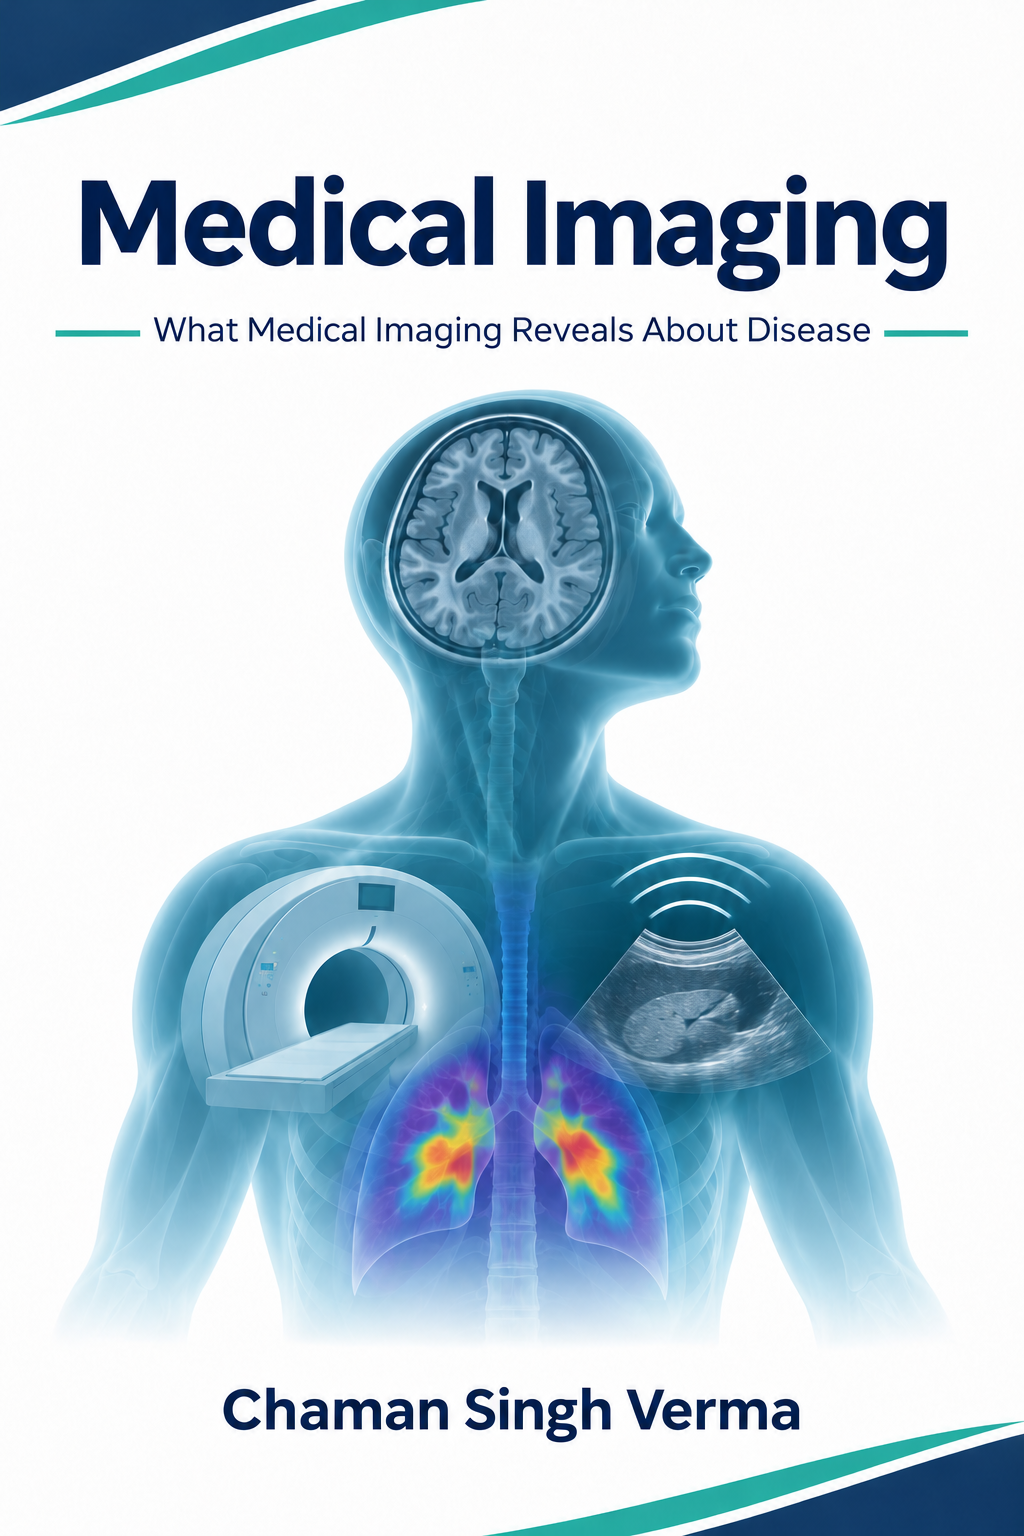
\includegraphics[height=0.96\textheight,width=0.96\textwidth,keepaspectratio]{medical_imaging_front_cover.png}
    \vspace*{\fill}
\end{titlepage}

% Copyright Page
\newpage
\thispagestyle{empty}
\vspace*{\fill}
\noindent \copyright\ 2026 Chaman Singh Verma. All rights reserved.\\[0.5cm]
\textbf{Disclaimer:} This book is for educational and reference purposes only.\\[0.5cm]
ISBN: To be assigned\\[0.5cm]
First Edition: 2026

% Dedication
\newpage
\thispagestyle{empty}
\vspace*{\fill}
\begin{center}
    \textit{To the radiologists, sonographers, technologists, and clinicians\\
    who turn images into insight and findings into diagnoses.}
\end{center}
\vspace*{\fill}

% Preface
\chapter*{Preface}
\addcontentsline{toc}{chapter}{Preface}
\markboth{Preface}{Preface}

Medical imaging makes disease visible through anatomy, tissue structure, physiology and molecular activity. This book focuses on what imaging reveals about disease: the findings each modality can show, how those findings relate to clinical questions, and where interpretation has limits.

\textbf{Organization:} The book moves from imaging principles and modalities to image interpretation, organ systems, disease patterns, emergencies, interventions, artificial intelligence, and practical diagnosis. Across these topics, the emphasis is on imaging appearance, diagnostic contribution, limitations and clinical context.

\vspace{1cm}
\noindent \textit{Chaman Singh Verma}\\\\\\\textit{2026}

% Medical safety and standards note
\chapter*{Medical Safety and Use of This Reference}
\addcontentsline{toc}{chapter}{Medical Safety and Use of This Reference}
\markboth{Medical Safety}{Medical Safety}

This book is an educational reference about medical imaging and disease. It is not a substitute for a radiologist's interpretation, a patient's treating clinician, or local institutional policy. Imaging choices, protocols, contrast decisions, radiation dose, sedation and follow-up must be individualized to the clinical question, patient characteristics, available equipment and current local guidance.

\section*{How to Use This Book}
Begin with the clinical question and the body region or disease under consideration. Review the relevant modality to understand what it measures, then compare the imaging findings with the clinical context. Use the interpretation and disease chapters to consider patterns, alternatives and limitations. Imaging findings support clinical assessment; they should be interpreted alongside symptoms, examination, laboratory results and the official report.

\begin{itemize}
    \item \textbf{Appropriateness:} Select imaging by the clinical question and expected effect on management. Evidence-based referral guidance can support the decision, but the referring clinician and radiologist remain responsible for the final choice.
    \item \textbf{Radiation:} Ionizing examinations require justification and optimization. Use the lowest exposure consistent with the diagnostic task; do not treat a nominal dose table as a patient-specific risk estimate.
    \item \textbf{Pregnancy and children:} Do not withhold clinically justified imaging solely because of pregnancy or age. Consider non-ionizing alternatives when diagnostically suitable, and optimize the examination using current local protocols.
    \item \textbf{Contrast media:} Screen for prior contrast reactions, relevant comorbidities, medications, pregnancy, and kidney function according to the agent and examination. Shellfish allergy is not a specific predictor of iodinated contrast reaction, and fasting is not universal.
    \item \textbf{MRI:} MRI safety depends on the exact implant, device, object, field strength, and conditions of use. Complete the facility's current screening, gowning, and final-check procedures before entering the controlled access zones.
    \item \textbf{Communication:} Critical or unexpected findings require prompt communication through the institution's documented escalation pathway. Examples in this book are educational and do not replace local critical-result policy.
\end{itemize}

The safety framework is informed by the American College of Radiology \textit{Manual on Contrast Media}, the ACR \textit{Manual on MR Safety}, the ACR \textit{Appropriateness Criteria}, and International Atomic Energy Agency principles of justification and optimization. These resources and local regulations should be checked for updates before clinical use.

\textbf{Core resources:} \url{https://www.acr.org/Clinical-Resources/Contrast-Manual}; \url{https://www.acr.org/Clinical-Resources/Radiology-Safety/MR-Safety}; \url{https://www.acr.org/Clinical-Resources/ACR-Appropriateness-Criteria}; \url{https://www.iaea.org/resources/rpop}; \url{https://www.radiologyinfo.org/en}; \url{https://www.nmc.org.in/information-desk/for-colleges/ug-curriculum/}

% Table of Contents
\setcounter{tocdepth}{0}
\tableofcontents

% List of Abbreviations
\chapter*{List of Abbreviations}
\addcontentsline{toc}{chapter}{List of Abbreviations}
\markboth{Abbreviations}{Abbreviations}

\begin{footnotesize}
\begin{longtable}{@{}ll@{}}
\toprule
\textbf{Abbreviation} & \textbf{Meaning} \\\\
\midrule
\endhead
ABG & Arterial blood gas \\\\
ANA & Antinuclear antibody \\\\
aPTT & Activated partial thromboplastin time \\\\
BMP & Basic metabolic panel \\\\
BNP & B-type natriuretic peptide \\\\
BUN & Blood urea nitrogen \\\\
CBC & Complete blood count \\\\
CK & Creatine kinase \\\\
CMP & Comprehensive metabolic panel \\\\
CRP & C-reactive protein \\\\
CT & Computed tomography \\\\
eGFR & Estimated glomerular filtration rate \\\\
ESR & Erythrocyte sedimentation rate \\\\
HbA1c & Glycated hemoglobin \\\\
LDH & Lactate dehydrogenase \\\\
MRI & Magnetic resonance imaging \\\\
POCT & Point-of-care testing \\\\
PSA & Prostate-specific antigen \\\\
PT/INR & Prothrombin time / International normalized ratio \\\\
TSH & Thyroid-stimulating hormone \\\\
UA & Urinalysis \\\\
\bottomrule
\end{longtable}
\end{footnotesize}

\mainmatter

% ============================================================
% PART I. FOUNDATIONS
% ============================================================
\part{Foundations}

\chapter{Introduction to Medical Imaging}

\section*{Patient focus}
This chapter explains the examination or clinical problem in accessible language. Patients should use it to prepare questions and understand the purpose, experience, benefits, and limitations of imaging; local instructions and the official report take priority.


\label{ch:intro}

Medical imaging is a cornerstone of modern clinical diagnosis, oncology staging, surgical planning, and therapeutic monitoring. By translating physical energy interactions with human tissues into spatial representations, medical imaging allows clinicians to visualize internal anatomy, physiological processes, and cellular metabolism non-invasively.

---

\section*{1. Classification of Medical Imaging Modalities}
Diagnostic imaging modalities can be classified using three primary criteria:

\subsection*{By Physical Energy Source}
\begin{itemize}
\item \textbf{Electromagnetic Radiation (X-rays)}: High-energy photons are projected through the body. Modalities include planar X-ray radiography, fluoroscopy, mammography, and computed tomography (CT).
\item \textbf{Mechanical Sound Waves}: High-frequency sound waves propagate through soft tissue, reflecting at acoustic boundaries. Modalities include grayscale ultrasound, Doppler flow analysis, and echocardiography.
\item \textbf{Magnetic Fields and Radiofrequency (RF) Waves}: Protons in tissue align with a magnetic field and are excited by RF pulses. Modalities include structural MRI, functional MRI (fMRI), and diffusion-weighted MRI.
\item \textbf{Radioactive Decay (Radiopharmaceuticals)}: Unstable isotopes bound to metabolic ligands are injected and detected. Modalities include SPECT and positron emission tomography (PET).
\end{itemize}

\subsection*{By Ionization Hazard}
\begin{itemize}
\item \textbf{Ionizing Modalities}: Utilize radiation of sufficient energy to liberate electrons from atoms, posing a biological risk of DNA damage. Includes X-ray, fluoroscopy, CT, SPECT, and PET.
\item \textbf{Non-Ionizing Modalities}: Do not utilize ionizing radiation. Includes ultrasound and MRI. Modality choice should be individualized, especially during pregnancy and in children.
\end{itemize}

\subsection*{By Clinical Objective: Structural vs. Functional}
\begin{itemize}
\item \textbf{Structural Imaging}: Focuses on detailed anatomical localization, boundaries, and physical densities (e.g., bones on CT, soft tissue borders on MRI, gallstones on ultrasound).
\item \textbf{Functional / Molecular Imaging}: Focuses on physiological activity, blood perfusion, receptor binding, and cellular metabolism (e.g., glucose consumption on FDG-PET, brain perfusion on fMRI, or ventilation-perfusion mismatch on V/Q scan).
\end{itemize}

---

\section*{2. The Clinical Imaging Workflow}
The imaging pathway is a multi-step clinical process requiring coordination between referring physicians, technologists, medical physicists, and radiologists:

\begin{enumerate}
    \item \textbf{Clinical Indication \& Question}: The referring physician identifies a clinical symptom or diagnostic question (e.g., ``Sudden onset left-sided weakness; rule out stroke'').
    \item \textbf{Modality Selection \& Appropriateness}: Selecting the optimal test. Guidelines (such as the ACR Appropriateness Criteria) help balance diagnostic yield against radiation dose, cost, contrast safety, and speed.
    \item \textbf{Patient Preparation \& Screening}: Screening for contraindications (e.g., checking renal function for contrast safety, or screening for metallic implants before MRI).
    \item \textbf{Image Acquisition}: The radiographer/technologist positions the patient and operates the scanner using optimized protocols.
    \item \textbf{Reconstruction \& Post-Processing}: Fusing datasets, generating reformations (axial, coronal, sagittal), or correcting artifacts.
    \item \textbf{Interpretation}: The radiologist systematically reviews the images, correlates findings with clinical history, and generates a structured report.
    \item \textbf{Clinical Communication}: Communicating findings to the clinical team, including immediate direct verbal reporting of critical or life-threatening results.
\end{enumerate}

\clearpage

\chapter{History of Medical Imaging}

\label{ch:ch02_history}

Medical imaging has transformed from a single accidental discovery into a vast ecosystem of modalities, each revealing a different facet of human anatomy and physiology. Understanding this history is not mere trivia; it explains why certain techniques exist, why some are preferred over others, and how the safeguards you use every day came to be.


\section*{1. Why Does the History Matter to Me?}
If you are a patient, knowing the history of imaging helps you understand:
\begin{itemize}
    \item Why your doctor orders one scan instead of another---each modality was invented to solve a different clinical problem.
    \item Why safety protocols exist---early radiologists suffered radiation burns because dosimetry was not yet understood.
    \item Why imaging has become safer and more precise over time---each generation of technology built on lessons from the last.
    \item Why some examinations involve contrast agents and others do not---contrast was developed to answer questions that plain images could not.
\end{itemize}
You do not need to memorise dates. What matters is that every imaging technique you encounter today exists because someone asked a clinical question that existing tools could not answer.


\section*{2. The Timeline of Major Milestones}

\subsection*{1895 --- Wilhelm R\"{o}ntgen and the Discovery of X-Rays}
On 8 November 1895, Wilhelm Conrad R\"{o}ntgen was experimenting with cathode-ray tubes when he noticed a fluorescent screen glowing across the room. He had discovered a new form of radiation that could pass through soft tissue but not bone. He named them ``X-rays'' (X for unknown). Within weeks he produced the famous image of his wife Anna Bertha's hand, clearly showing the bones and her wedding ring. In 1901, R\"{o}ntgen received the first-ever Nobel Prize in Physics.

\begin{pearlbox}[First clinical use]
The first clinical X-ray was performed on a patient with a fractured wrist in 1896. The image took nearly 20 minutes of exposure. Modern radiography exposes a patient for milliseconds.
\end{pearlbox}

\subsection*{1896--1950s --- Early Radiography and Fluoroscopy}
Following R\"{o}ntgen's discovery, X-ray departments appeared in hospitals worldwide within a few years. Early radiology was dangerous: operators had no concept of radiation dose, and many pioneering radiologists developed radiation dermatitis and cancers. Key developments of this era included:
\begin{itemize}
    \item \textbf{Fluoroscopy} (1896): Real-time X-ray imaging using a fluorescent screen, enabling the study of motion (heartbeat, swallowing, bowel peristalsis).
    \item \textbf{Image intensification} (1940s--50s): Dramatically reduced the dose needed for fluoroscopy and produced brighter images.
    \item \textbf{Barium contrast} (1910s): Barium sulphate allowed visualisation of the gastrointestinal lumen for the first time.
    \item \textbf{Iodinated contrast} (1920s--30s): Enabled angiography and excretory urography.
    \item \textbf{Dosimetry and radiation protection} (1920s--50s): Recognition of radiation hazards led to the concept of maximum permissible dose and the establishment of protective standards.
\end{itemize}

\subsection*{1950s -- 1970s --- Ultrasound Enters the Clinic}
During World War II, sonar technology was developed to detect submarines. In the 1950s, Ian Donald (Glasgow) adapted pulsed ultrasound for obstetric imaging, producing the first foetal images. By the 1960s, real-time B-mode scanning was available, and by the 1970s, grey-scale ultrasound had become routine for abdominal, pelvic, and obstetric imaging.

Key contributions:
\begin{itemize}
    \item No ionising radiation---safe for pregnancy and children.
    \item Portable and relatively inexpensive.
    \item Real-time imaging of dynamic processes (cardiac valves, foetal movement, blood flow with Doppler).
\end{itemize}

\subsection*{1971 --- Godfrey Hounsfield and Computed Tomography (CT)}
Godfrey Hounsfield (EMI Ltd) built the first clinical CT scanner, which performed its first patient scan at Atkinson Morley Hospital, London, in 1971. Allan Cormack (Tufts University) independently developed the mathematical theory behind CT image reconstruction. Together they shared the 1979 Nobel Prize in Physiology or Medicine.

\begin{pearlbox}[Why CT was revolutionary]
Conventional radiography superimposes all structures onto a single 2D image. CT uses rotating X-ray beams and computer reconstruction to produce cross-sectional ``slices,'' eliminating tissue overlap and vastly improving the detection of lesions in the brain, chest, abdomen, and musculoskeletal system. The Hounsfield Unit scale, named after Godfrey Hounsfield, remains the standard for quantifying tissue density on CT.
\end{pearlbox}

Key CT milestones:
\begin{itemize}
    \item \textbf{1971}: First clinical CT scan (head only, scan time ~5 minutes per slice).
    \item \textbf{1974}: First whole-body CT scanner.
    \item \textbf{1970s--80s}: Second- and third-generation CT designs reduced scan times to seconds.
    \item \textbf{1989}: Spiral (helical) CT---continuous table movement during acquisition.
    \item \textbf{1998}: Multi-detector CT (MDCT)---multiple rows of detectors enabled sub-millimetre resolution and faster coverage.
    \item \textbf{2000s--present}: Dual-energy CT, CT perfusion, cardiac CT, and low-dose techniques.
\end{itemize}

\subsection*{1970s -- 1980s --- Magnetic Resonance Imaging (MRI)}
The principles of nuclear magnetic resonance (NMR) were described by Bloch and Purcell in the 1940s (Nobel Prize, 1952). Raymond Damadian (1971) demonstrated that tumor tissue had different NMR relaxation times from normal tissue. Paul Lauterbur developed gradient-based spatial encoding (1973), and Peter Mansfield refined the mathematics of image reconstruction. Lauterbur and Mansfield shared the 2003 Nobel Prize in Physiology or Medicine.

MRI entered clinical use in the early 1980s and rapidly became the modality of choice for:
\begin{itemize}
    \item Brain and spinal cord imaging (superior soft-tissue contrast).
    \item Joint and musculoskeletal imaging (cartilage, ligaments, tendons).
    \item Cardiac imaging (viability, perfusion, function).
    \item Abdominal and pelvic organ characterisation.
\end{itemize}
Unlike CT, MRI uses no ionising radiation. Risks relate primarily to the strong magnetic field (ferromagnetic implants, pacemakers) and, for some agents, gadolinium deposition in the brain and kidneys.

\subsection*{1970s -- 1990s --- Nuclear Medicine: SPECT and PET}
Nuclear medicine uses radiopharmaceuticals (tracers) to image physiological processes rather than anatomy alone.
\begin{itemize}
    \item \textbf{SPECT (Single Photon Emission Computed Tomography)}: Uses gamma-emitting isotopes (e.g., $^{99m}$Tc) for cardiac perfusion imaging, bone scans, and brain perfusion studies.
    \item \textbf{PET (Positron Emission Tomography)}: Uses positron-emitting isotopes (most commonly $^{18}$F-FDG, a glucose analogue) to map metabolic activity. PET-CT, combining metabolic and anatomic information, became the standard for cancer staging in the 2000s. More recently, PET-MRI has emerged for combined metabolic and high soft-tissue contrast imaging.
\end{itemize}

\subsection*{1990s -- 2000s --- Digital Radiography and PACS}
Film-screen radiography was the norm for nearly a century. The transition to digital imaging happened in two streams:
\begin{itemize}
    \item \textbf{Computed Radiography (CR)}: Phosphor plates replace film cassettes; images are read by a laser scanner and sent digitally to PACS.
    \item \textbf{Direct Radiography (DR)}: Flat-panel detectors convert X-rays directly to digital signals, offering faster acquisition and lower dose.
\end{itemize}
The Picture Archiving and Communication System (PACS) enabled digital storage, retrieval, and distribution of images, eliminating the need for physical film. The DICOM standard (see Chapter~\ref{ch:ch09_pacs_dicom}) ensured interoperability between scanners, storage systems, and viewers from different manufacturers.

\subsection*{2000s -- Present --- Interventional and Hybrid Imaging}
\begin{itemize}
    \item \textbf{Interventional radiology} matured into a full clinical specialty, offering image-guided biopsies, drainages, angioplasty, stenting, embolization, and ablation.
    \item \textbf{Hybrid imaging} (PET-CT, PET-MRI, SPECT-CT) combines functional and anatomic information in a single examination.
    \item \textbf{Photon-counting CT} (2020s) uses semiconductor detectors that count individual photons, enabling lower dose, higher resolution, and material decomposition.
\end{itemize}

\subsection*{2020s --- Artificial Intelligence and the Current Frontier}
AI (see Chapter~\ref{ch:ch10_ai_intro}) is being integrated into nearly every aspect of imaging: automated detection, triage, segmentation, structured reporting, and quality assurance. While AI does not replace the radiologist, it augments human interpretation and promises to reduce errors, improve throughput, and extend specialist-level interpretation to underserved settings.


\section*{3. How Technology Changed Clinical Practice}

\begin{table}[h]
\centering
\caption{How each modality changed the dominant clinical question}
\begin{tabular}{|p{3cm}|p{5cm}|p{5cm}|}
\hline
\textbf{Modality} & \textbf{Clinical question answered} & \textbf{Impact on practice} \\
\hline
AI tools & Can detection, triage, or reporting be automated? & Augments radiologist performance; enables triage of critical findings. \\
\hline
CT & What is the detailed cross-sectional anatomy and where is the pathology? & Transformed emergency medicine (trauma, stroke, PE) and cancer staging. \\
\hline
Fluoroscopy & How does the GI tract or vascular system function in real time? & Enabled barium studies, angiography, and interventional procedures. \\
\hline
Interventional radiology & Can I diagnose and treat without open surgery? & Created minimally invasive alternatives to surgery across many specialties. \\
\hline
MRI & What is the tissue characterisation and functional status? & Replaced CT as first-line for brain, spine, joints, and many abdominal indications. \\
\hline
Nuclear medicine & What is the metabolic or physiological activity? & Enabled bone scanning, cardiac perfusion, and PET-CT cancer staging. \\
\hline
Radiography & Is there a fracture, pneumonia, or abnormal mass? & Became the first-line investigation for chest and skeletal complaints. \\
\hline
Ultrasound & What is the structure and flow of soft-tissue organs? & Replaced exploratory surgery in many abdominal and obstetric contexts. \\
\hline
\end{tabular}
\end{table}


\section*{4. Nobel Prizes in Medical Imaging}
\begin{table}[h]
\centering
\caption{Nobel Prizes awarded for work directly related to medical imaging}
\begin{tabular}{|l|l|p{5cm}|}
\hline
\textbf{Year} & \textbf{Recipient(s)} & \textbf{Contribution} \\
\hline
1901 & Wilhelm R\"{o}ntgen & Discovery of X-rays. \\
\hline
1952 & Felix Bloch, Edward Purcell & Nuclear magnetic resonance (foundation of MRI). \\
\hline
1979 & Godfrey Hounsfield, Allan Cormack & Development of computed tomography (CT). \\
\hline
2003 & Paul Lauterbur, Peter Mansfield & Discoveries concerning magnetic resonance imaging (MRI). \\
\hline
\end{tabular}
\end{table}


\section*{5. The Safety Lessons of History}
The history of imaging is also a history of learning from mistakes:
\begin{itemize}
    \item \textbf{Early radiologists} suffered radiation burns, amputations, and cancers before dosimetry and shielding were understood. Many died young.
    \item \textbf{Thalidomide (1950s--60s)} highlighted the need for strict protocols around imaging in pregnancy.
    \item \textbf{Iodinated contrast reactions} were far more common and severe with early ionic, high-osmolality agents. The development of non-ionic, low-osmolality contrast in the 1980s dramatically reduced reaction rates.
    \item \textbf{Gadolinium deposition} (identified in the 2010s) led to revised guidance on the use of linear gadolinium agents in patients with impaired renal function.
    \item \textbf{CT radiation dose awareness} (2000s--present) prompted dose optimisation campaigns (Image Gently, Image Wisely) and the development of low-dose and photon-counting CT.
\end{itemize}

\begin{warnbox}[The past is not the present]
A patient who had a bad reaction to contrast ``20 years ago'' may be reacting to an agent class that is no longer used. Always obtain specific details about the prior reaction, but do not assume that current agents carry the same risk.
\end{warnbox}


\section*{6. Key Dates at a Glance}

\begin{table}[h]
\centering
\caption{Timeline of major milestones in medical imaging}
\begin{tabular}{|l|p{10cm}|}
\hline
\textbf{Year} & \textbf{Milestone} \\
\hline
1895 & R\"{o}ntgen discovers X-rays. \\
\hline
1896 & First clinical radiograph; first use of fluoroscopy. \\
\hline
1910s & Barium contrast for GI imaging. \\
\hline
1920s--30s & Iodinated contrast agents; radiation protection standards. \\
\hline
1940s--50s & Image intensification for fluoroscopy; NMR discovered. \\
\hline
1950s & Ian Donald pioneers obstetric ultrasound. \\
\hline
1960s--70s & Real-time ultrasound; grey-scale imaging. \\
\hline
1971 & First clinical CT scan (Hounsfield). \\
\hline
1973 & Lauterbur proposes gradient-based MRI. \\
\hline
1977 & First clinical MRI scan. \\
\hline
1980s & Clinical MRI enters routine use. \\
\hline
1989 & Spiral CT introduced. \\
\hline
1990s & Digital radiography (CR and DR); PACS deployment. \\
\hline
1998 & Multi-detector CT (MDCT). \\
\hline
2000s & PET-CT becomes standard for cancer staging; PACS widespread. \\
\hline
2010s & Dual-energy CT; AI research accelerates. \\
\hline
2020s & Photon-counting CT; AI clinical deployment; PET-MRI. \\
\hline
\end{tabular}
\end{table}


\section*{7. What This Means for You as a Clinician}
Each imaging modality was invented because a clinician had a question that existing tools could not answer. When you order an imaging study, you are drawing on over 130 years of accumulated knowledge, safety refinement, and technological innovation. Your responsibility is to:
\begin{itemize}
    \item Ask the right clinical question before choosing the modality.
    \item Understand the strengths and limitations of each technique.
    \item Apply safety protocols that were written because others learned from adverse events.
    \item Recognize that the ``best'' imaging is not the most advanced, but the one that answers the clinical question safely and efficiently.
\end{itemize}

\begin{pearlbox}[The best technology is the one that answers the question]
The history of medical imaging teaches humility. Each generation believed its tools were the pinnacle; each generation was proved wrong by the next. What endures is not the technology but the principle: match the modality to the clinical question, prioritise patient safety, and never stop learning.
\end{pearlbox}

\clearpage

\chapter{Physics of Medical Imaging}

\label{ch:physics}

Medical imaging modalities rely on the interaction of different forms of energy (electromagnetic radiation, acoustic waves, and nuclear magnetic resonance) with human tissue. This chapter details the physical principles underlying the major imaging modalities: X-ray/CT, Ultrasound, MRI, and Nuclear Medicine.


\section*{1. X-Ray and CT Physics: Ionizing Electromagnetic Radiation}
X-rays are high-energy photons on the electromagnetic spectrum, exhibiting wave-particle duality.

\subsection*{X-Ray Production}
X-rays are produced inside an evacuated tube containing a tungsten cathode (filament) and a rotating tungsten anode:
\begin{enumerate}
    \item \textbf{Thermionic Emission:} Current passes through the cathode filament, heating it and releasing a cloud of electrons.
    \item \textbf{Acceleration:} A high voltage (typically 50--140 peak kilovoltage, kVp) is applied between the cathode and anode, accelerating electrons toward the anode.
    \item \textbf{Target Interaction (Bremsstrahlung and Characteristic Radiation):} The high-speed electrons strike the anode, converting most of their kinetic energy into heat ($\approx 99\%$) and a small fraction into X-ray photons ($\approx 1\%$). Two mechanisms produce X-rays:
    \begin{itemize}
        \item \textbf{Bremsstrahlung (Braking Radiation):} Rapid deceleration of incident electrons deflected by the positive electric field of anode nuclei produces a continuous spectrum of X-ray energies.
        \item \textbf{Characteristic X-rays:} Incident high-speed electrons collide with and eject inner-shell (K-shell) electrons from anode atoms. Outer-shell electrons drop into the vacancy, emitting photons with discrete, element-specific energies.
    \end{itemize}
\end{enumerate}

\subsection*{X-Ray Interaction with Matter}
As X-ray photons pass through tissue, they are attenuated (absorbed or scattered) via two primary diagnostic interactions:
\begin{itemize}
    \item \textbf{Photoelectric Effect}: An incoming photon is completely absorbed by an inner-shell electron of a tissue atom, ejecting the electron. This interaction depends strongly on the atomic number of the tissue ($Z^3$). Bone (high calcium, $Z=20$) absorbs much more than soft tissue ($Z \approx 7$), creating contrast.
    \item \textbf{Compton Scattering}: An incoming photon collides with an outer-shell tissue electron, ejecting the electron and scattering the photon in a new direction with lower energy. Compton scattering is the primary source of scatter radiation, which degrades image quality and increases occupational radiation dose.
\end{itemize}


\section*{2. Ultrasound Physics: Acoustic Wave Propagation}
Ultrasound uses mechanical longitudinal sound waves (frequencies between 2 and 18 MHz) that propagate through physical media.

\subsection*{Generation and Detection: The Piezoelectric Effect}
\begin{itemize}
    \item \textbf{Transducer Crystals}: Made of piezoelectric materials (like lead zirconate titanate or PZT).
    \item \textbf{Piezoelectric Effect}: When an electrical voltage is applied to the crystal, it vibrates and produces sound waves (mechanical energy). Conversely, when returning sound waves strike the crystal, it deforms and generates an electrical signal that is processed into an image.
\end{itemize}

\subsection*{Propagation and Acoustic Impedance}
Ultrasound systems assume an average acoustic speed of \textbf{1,540 m/s} in soft tissue to convert echo arrival time into depth (though actual speeds vary slightly by tissue). Contrast is formed at boundaries between tissues of different \textbf{Acoustic Impedance ($Z$)}:
\[
Z = \rho \cdot c
\]
where $\rho$ is tissue density and $c$ is sound velocity.
\begin{itemize}
    \item \textbf{Reflection}: When sound hits a boundary between two tissues of different $Z$, a portion of the wave is reflected back to the probe. The amount of reflection is proportional to the difference in impedance ($\Delta Z$).
    \item \textbf{Acoustic Mismatch}: The interface between soft tissue and air or bone has an extremely large $\Delta Z$. This causes nearly 100\% reflection, preventing sound propagation and explaining why ultrasound cannot image through air (requiring gel) or bone.
\end{itemize}


\section*{3. MRI Physics: Nuclear Magnetic Resonance}
MRI relies on the magnetic properties of hydrogen nuclei (single protons), which are highly abundant in water and fat.

\subsection*{Spin and Precession}
Hydrogen nuclei possess an intrinsic quantum property called \textbf{spin}, giving them a magnetic dipole moment.
\begin{enumerate}
    \item \textbf{Alignment:} When placed in a strong external magnetic field ($B_0$), proton spins align preferentially with or against $B_0$, creating a net longitudinal magnetization vector ($M_0$).
    \item \textbf{Precession:} Protons precess around the axis of $B_0$ at the \textbf{Larmor Frequency ($f_0$)}:
    \[
    f_0 = \bar{\gamma} \cdot B_0
    \]
    where $\bar{\gamma} = \gamma/(2\pi) \approx 42.58\text{ MHz/Tesla}$ for hydrogen (or $\omega_0 = \gamma B_0$ in rad/s).
\end{enumerate}

\subsection*{Excitation and Relaxation}
\begin{itemize}
    \item \textbf{Excitation}: An RF (radiofrequency) pulse is applied at the Larmor frequency. Protons absorb this energy (resonance), tilting the net magnetization vector into the transverse plane ($xy$-plane).
    \item \textbf{Relaxation}: When the RF pulse is turned off, protons return to equilibrium, emitting the absorbed RF energy:
    \item \textbf{T1 Relaxation (Spin-Lattice)}: Recovery of longitudinal magnetization ($M_z$) as protons transfer energy to the surrounding lattice.
    \item \textbf{T2 Relaxation (Spin-Spin)}: Decay of transverse magnetization ($M_{xy}$) due to loss of phase coherence (dephasing) among precessing protons.
\end{itemize}


\section*{4. Nuclear Medicine Physics: Radioactive Decay}
Nuclear medicine utilizes unstable atomic nuclei (radionuclides) that undergo spontaneous decay to achieve stability.

\subsection*{Decay Modalities}
\begin{itemize}
    \item \textbf{Gamma Decay}: An excited nucleus releases energy as high-energy electromagnetic radiation (gamma photons). Used in single-photon emission computed tomography (SPECT; e.g., technetium-99m, which has a 6-hour half-life and emits 140 keV photons).
    \item \textbf{Positron Emission ($\beta^+$ decay)}: A proton inside the nucleus decays into a neutron, a positron ($\beta^+$), and a neutrino. Used in positron emission tomography (PET; e.g., fluorine-18).
    \item \textbf{Annihilation}: The emitted positron travels 1--2 mm in tissue before colliding with a tissue electron. The mass of both particles is converted into two \textbf{511 keV gamma photons} emitted $180^\circ$ apart. Coincidence detection of these photon pairs allows PET reconstruction.
\end{itemize}

\clearpage

\chapter{Image Formation}

\label{ch:image_formation}

Image formation is the physical and mathematical process of converting raw energy signals—whether X-ray photons, acoustic echoes, or radiofrequency waves—into digital pixels (2D) and voxels (3D) that clinicians can interpret. This chapter details the image formation mechanisms of radiography, CT, ultrasound, and MRI.


\section*{1. Projection Radiography (X-Ray) Image Formation}
Planar X-ray image formation relies on differential attenuation of X-ray photons as they pass through the patient, creating a shadowgram.

\subsection*{Geometric Principles}
\begin{itemize}
    \item \textbf{Focal Spot Size}: X-rays emerge from a focal spot on the anode. A smaller focal spot reduces geometric blurring (penumbra) and increases spatial resolution, but increases heat concentration.
    \item \textbf{Scatter Reduction (Grids)}: Scatter photons (Compton scattering) degrade image contrast. An anti-scatter grid (thin lead strips) is placed between the patient and the detector, allowing primary perpendicular photons to pass while blocking angled, scattered photons.
\end{itemize}

\subsection*{Digital Detectors}
\begin{itemize}
    \item \textbf{Computed Radiography (CR)}: Uses a photostimulable phosphor (PSP) plate that traps electrons in a meta-stable state when exposed to X-rays. The plate is scanned by a red laser in a reader, releasing the stored energy as blue light (photostimulated luminescence), which is converted into a digital signal.
    \item \textbf{Digital Radiography (DR)}: Uses flat-panel detectors that provide immediate image readout:
\end{itemize}
  \begin{itemize}
      \item \textbf{Indirect Conversion}: X-rays strike a scintillator (e.g., cesium iodide) that converts X-rays to visible light. A photodiode array (amorphous silicon) then converts light into electrical charge.
      \item \textbf{Direct Conversion}: X-rays strike a photoconductor (amorphous selenium) that directly converts photons into electrical charge, avoiding light diffusion and providing superior spatial resolution.
  \end{itemize}


\section*{2. Computed Tomography (CT) Reconstruction}
CT scanners acquire thousands of projection profiles (shadowgrams) at multiple angles around the patient.

\subsection*{The Radon Transform and Sinograms}
\begin{itemize}
    \item \textbf{Sinogram}: The raw data space of a CT scan. The mathematical projection of tissue attenuation values at different angles is called the \textbf{Radon Transform}. Fusing these profiles creates a sinogram.
    \item \textbf{Reconstruction}: Reconstructing the sinogram back into a cross-sectional axial image requires mathematical algorithms.
\end{itemize}

\subsection*{Reconstruction Algorithms}
\begin{itemize}
    \item \textbf{Filtered Backprojection (FBP)}: The classical algorithm. Attenuation values are smeared back across the image matrix. A mathematical filter is applied to remove blurring. While FBP is fast, it generates significant image noise at low radiation doses.
    \item \textbf{Iterative Reconstruction (IR)}: A family of methods that repeatedly compares measured projection data with predicted data from the current image estimate. These methods can reduce noise and may support dose optimization, but the achievable dose change depends on the scanner, reconstruction method, anatomy, protocol, and diagnostic task. There is no universal dose-reduction percentage, and image texture or spatial resolution may change.
\end{itemize}


\section*{3. Ultrasound Image Formation}
Ultrasound images are built slice-by-slice by transmitting sound pulses and listening for echoes.

\subsection*{Pulse-Echo Ranging}
The ultrasound system calculates the depth of a reflecting tissue interface based on the \textbf{round-trip time} ($t$) of the sound wave:
$$\text{Depth} = \frac{c \cdot t}{2}$$
where $c$ is the velocity of sound in tissue (1540 m/s). 

\subsection*{Time-Gain Compensation (TGC)}
As sound waves travel deeper, they undergo attenuation (loss of energy due to absorption and scattering). Without compensation, deeper structures would appear dark. \textbf{Time-Gain Compensation (TGC)} amplifies returning signals selectively based on their arrival time, ensuring uniform brightness across the depth of the image.


\section*{4. MRI Spatial Encoding: K-Space to Image}
MRI reconstruction is purely mathematical and relies on modifying the magnetic field to tag proton locations with specific frequencies and phases.

\subsection*{Spatial Encoding Gradients}
Three orthogonal magnetic gradients ($G_x, G_y, G_z$) are superimposed on $B_0$:
1. \textbf{Slice Selection Gradient ($G_z$)}: Modifies the magnetic field along the $z$-axis. When an RF pulse matching the Larmor frequency at a specific position is applied, only protons in that specific slice are excited.
2. \textbf{Phase Encoding Gradient ($G_y$)}: Temporarily applied along the $y$-axis, causing protons to precess at different speeds. When the gradient is turned off, they return to the same frequency but retain different \textbf{phase angles}.
3. \textbf{Frequency (Readout) Encoding Gradient ($G_x$)}: Applied along the $x$-axis during signal readout, causing protons to precess at different \textbf{frequencies} depending on their position.

\subsection*{K-Space and the Fourier Transform}
\begin{itemize}
    \item \textbf{K-Space}: The raw data matrix where MRI signals are stored during acquisition. Each point in K-space represents a spatial frequency, not a physical pixel.
    \item \textbf{Reconstruction}: Once K-space is fully filled, a mathematical operation called the \textbf{2D Inverse Fast Fourier Transform (2D-IFFT)} is applied to convert the spatial frequencies of K-space into the final anatomical grayscale image.
\end{itemize}

\clearpage

\chapter{Image Quality}

\section*{Patient focus}
This chapter explains the examination or clinical problem in accessible language. Patients should use it to prepare questions and understand the purpose, experience, benefits, and limitations of imaging; local instructions and the official report take priority.


\label{ch:image_quality}

Diagnostic accuracy relies on the quality of the acquired image. An image must have sufficient detail, contrast, and clarity to allow a radiologist to differentiate subtle pathologies from normal tissues. This chapter defines the core parameters of image quality—spatial, contrast, and temporal resolution—and reviews the factors that degrade them.

---

\section*{1. Core Parameters of Image Quality}

\subsection*{Spatial Resolution}
Spatial resolution is the ability of an imaging system to distinguish two high-contrast objects placed close together as separate entities. 
\textbullet \textbf{Measurement}: Quantified in line pairs per millimeter (lp/mm) or by the \textbf{Modulation Transfer Function (MTF)}.
\textbullet \textbf{Modality Comparison}: Mammography and planar X-ray have the highest spatial resolution ($\approx 15$ lp/mm), while Nuclear Medicine (PET/SPECT) has the lowest ($\approx 0.1$ lp/mm).
\textbullet \textbf{Limiting Factors}: Pixel size in digital detectors, focal spot size in X-ray tubes, and reconstruction slice thickness.

\subsection*{Contrast Resolution}
Contrast resolution is the ability to distinguish subtle differences in soft tissue density or signal intensity, even if the structures are adjacent.
\textbullet \textbf{Modality Comparison}: MRI has the highest contrast resolution, followed by CT. Planar X-ray has poor contrast resolution because all overlapping soft tissues are projected onto a single 2D plane.
\textbullet \textbf{Measurement}: Described by the \textbf{Contrast-to-Noise Ratio (CNR)}.

\subsection*{Temporal Resolution}
Temporal resolution is the ability to capture motion or rapid physiological changes without motion blur.
\textbullet \textbf{Modality Comparison}: Ultrasound has excellent temporal resolution, displaying real-time movement (up to 100 frames/second). Cardiac CT utilizes rapid gantry rotation times ($< 250$ ms) and ECG-gating to image the beating heart without blur.
\textbullet \textbf{Limiting Factors}: Scanner acquisition speed and detector response times.

---

\section*{2. Noise: The Signal-to-Noise Ratio (SNR)}
Image noise is the random, unwanted variation in pixel values that degrades image clarity, appearing as a "grainy" or "sandy" texture (mottle):

\textbullet \textbf{Quantum Mottle}: The most common source of noise in X-ray and CT. It is caused by an insufficient number of X-ray photons reaching the detector. If the dose (photon count) is too low, the image will appear highly grainy, obscuring subtle structures.
\textbullet \textbf{Overcoming Noise}: In X-ray/CT, noise is reduced by increasing the tube current-time product (mAs) or using iterative reconstruction. In MRI, noise is reduced by increasing the number of excitations (NEX) or utilizing larger voxel volumes, though this increases scan time or reduces spatial resolution.

---

\section*{3. Factors Degrading Image Quality}
\textbullet \textbf{Geometric Blurring (Penumbra)}: Caused by the finite size of the X-ray tube focal spot. It is minimized by keeping the patient as close to the detector as possible (minimizing object-to-detector distance).
\textbullet \textbf{Patient Motion}: Blurs anatomical boundaries. Minimized via patient coaching, physical immobilization, rapid acquisition sequences, or motion-correction algorithms.
\textbullet \textbf{Artifacts}: Systemic distortions (e.g. beam hardening in CT, chemical shift or metallic susceptibility in MRI, reverberation in ultrasound) that can mimic or obscure pathology.

---

\section*{4. The Imaging Triad: Quality vs. Safety vs. Time}
Every imaging acquisition requires balancing three competing factors:
1. \textbf{Diagnostic Quality}: Achieving high spatial and contrast resolution.
2. \textbf{Patient Safety / Dose}: In ionizing modalities (CT/X-ray), increasing image quality (lower noise) requires increasing the radiation dose, which must be balanced against the \textbf{ALARA (As Low As Reasonably Achievable)} safety principle.
3. \textbf{Acquisition Time}: In MRI, higher resolution or SNR requires longer scan times, which increases the likelihood of patient motion artifacts and reduces scanner throughput.

\clearpage

\chapter{Contrast Agents}

\label{ch:ch06_contrast_agents}

Contrast agents are substances introduced into the body to enhance the visibility of structures or fluids on imaging. They do not treat disease; they make anatomy and pathology more visible so that the correct diagnosis can be made. This chapter covers the major classes of contrast agents, how they work, how they are administered, and how to manage adverse reactions.


\section*{1. What Contrast Feels Like and Why It Is Used}
If you are a patient about to receive contrast, here is what to expect:
\begin{itemize}
    \item \textbf{Intravenous (IV) contrast}: You will feel a brief, warm flush spreading through your body and a metallic taste in your mouth. This is normal and passes within 30--60 seconds. You may also feel the need to urinate; this is the kidneys filtering the contrast and is not dangerous.
    \item \textbf{Oral contrast (barium or iodinated)}: You drink a chalky or mildly flavoured liquid. It may cause bloating or mild nausea. You may need to drink it over 1--2 hours before the scan.
    \item \textbf{Rectal contrast}: Administered as an enema; similar sensation to a standard enema.
    \item \textbf{Intra-articular contrast}: Injected directly into a joint (e.g., MRI arthrogram); local anesthetic is used first to minimize discomfort.
\end{itemize}

Contrast is used to:
\begin{itemize}
    \item Highlight blood vessels (angiography).
    \item Distinguish normal from abnormal tissue in organs such as the liver, kidneys, and brain.
    \item Show whether a structure is fluid-filled, solid, or vascular.
    \item Assess organ function (e.g., renal excretion, blood-brain barrier integrity).
\end{itemize}


\section*{2. Iodinated Contrast Agents}
Iodinated contrast is the most commonly used class of IV contrast worldwide, primarily for CT and fluoroscopic angiography.

\subsection*{How They Work}
Iodine has a high atomic number (53), which attenuates X-rays much more effectively than soft tissue. By attaching iodine atoms to an organic carrier molecule, a water-soluble compound is created that remains in the extracellular space and is excreted by the kidneys.

\subsection*{Classification}

\begin{table}[h]
\centering
\caption{Iodinated contrast agent classification}
\begin{tabular}{|p{0.15\textwidth}|p{0.11\textwidth}|p{0.21\textwidth}|p{0.37\textwidth}|}
\hline
\textbf{Type} & \textbf{Osmolality} & \textbf{Example} & \textbf{Key features} \\
\hline
Ionic, high-osmolality (HOCM) & $\sim$1500--2000 mOsm/kg & Diatrizoate (Urografin) & Largely historical; higher reaction rate. \\
\hline
Ionic, low-osmolality (LOCM) & $\sim$600--800 mOsm/kg & Ioxaglate (Hexabrix) & Lower reaction rate than HOCM. \\
\hline
Non-ionic, iso-osmolality (IOCM) & $\sim$290 mOsm/kg & Iodixanol (Visipaque) & Osmolality similar to blood; no established clinically meaningful kidney-safety advantage over modern low-osmolality agents for routine IV CT. \\
\hline
Non-ionic, low-osmolality (LOCM) & $\sim$600--800 mOsm/kg & Iohexol (Omnipaque), Iopamidol (Isovue), Iopromide (Ultravist) & Current standard of care; lowest reaction rate. \\
\hline
\end{tabular}
\end{table}

\begin{pearlbox}[Shellfish and contrast]
A shellfish allergy does not specifically predict an iodinated contrast reaction. The historical rationale (both contain iodine) is a myth. Allergies to shellfish are related to tropomyosin, not iodine. Always ask about prior contrast reactions, but do not assume shellfish allergy is a risk factor for contrast reactions.
\end{pearlbox}

\subsection*{Routes of Administration}
\begin{itemize}
    \item \textbf{Intravenous}: Most common. Bolus injection via a peripheral IV cannula (typically 18--20G in the antecubital fossa). Power injection rates range from 1--5 mL/s depending on the study.
    \item \textbf{Oral}: Used for CT abdomen/pelvis to opacify the GI tract. Iodinated water-soluble agents are preferred over barium when there is a risk of perforation.
    \item \textbf{Rectal}: Used in selected CT protocols (e.g., CT colonography with stool tagging).
    \item \textbf{Intra-articular}: For CT or MRI arthrography.
    \item \textbf{Intrathecal}: For myelography (CT myelogram).
\end{itemize}


\section*{3. Gadolinium-Based Contrast Agents (GBCAs)}
GBCAs are used in MRI to highlight vascularity, blood-brain barrier breakdown, and tissue perfusion. Gadolinium is a paramagnetic metal that shortens T1 relaxation time, causing bright signal on T1-weighted images.

\subsection*{ACR Risk Groups for Gadolinium-Based Contrast Agents}

\begin{table}[h]
\centering
\caption{ACR groups used to describe NSF risk; the groups are not a simple structural classification. Verify the current agent-specific listing before clinical use.}
\begin{tabular}{|p{0.12\textwidth}|p{0.30\textwidth}|p{0.44\textwidth}|}
\hline
\textbf{ACR group} & \textbf{NSF risk category} & \textbf{Examples} \\
\hline
Group I & Highest established NSF association; includes linear agents & Gadodiamide (Omniscan), gadoversetamide (OptiMARK), gadopentetate dimeglumine (Magnevist) \\
\hline
Group II & Very low NSF risk; includes agents with different structures & Gadoterate (Dotarem), gadobutrol (Gadavist), gadoteridol (ProHance), gadobenate dimeglumine (MultiHance) \\
\hline
Group III & Limited data; agent-specific guidance applies & Gadoxetate disodium (Eovist/Primovist) \\
\hline
\end{tabular}
\end{table}

\begin{warnbox}[Nephrogenic Systemic Fibrosis (NSF)]
NSF has been strongly associated with ACR Group I agents in patients with severe renal impairment. Group II agents have a very low risk, and a clinically indicated Group II examination generally should not be withheld solely because eGFR is below 30 mL/min/1.73 m$^2$. Group III agents have more limited data and require agent-specific assessment. Use the current ACR group listing and local policy; do not infer risk from linear or macrocyclic structure alone.
\end{warnbox}

\subsection*{Gadolinium Deposition}
Gadolinium retention in tissues, including the brain, has been reported after GBCA administration and is generally greater with some linear agents than with macrocyclic agents. No adverse health effect has been established from retention in patients with normal renal function. Use contrast when clinically justified and avoid unnecessary repeated doses; do not delay needed imaging solely because of retention concerns.
\begin{itemize}
    \item Agent selection according to the indication, current safety guidance, and local formulary.
    \item Individual assessment when repeated contrast-enhanced examinations are anticipated.
    \item Recognition that regulatory restrictions differ by country and agent.
\end{itemize}


\section*{4. Microbubble Contrast (Ultrasound)}
Microbubble contrast agents (e.g., SonoVue/Lumason [sulphur hexafluoride], Definity [perflutren]) consist of tiny gas-filled microspheres (1--10 $\mu$m) stabilised by a phospholipid shell. They remain entirely within the intravascular space and oscillate when exposed to ultrasound, producing a strong non-linear signal that dramatically improves blood pool visualisation.

Clinical applications:
\begin{itemize}
    \item Characterisation of liver lesions (FLL-5 classification).
    \item Evaluation of cardiac wall motion and myocardial perfusion.
    \item Vascular assessment (e.g., testicular, carotid).
    \item Avoidance of CT/MRI in patients who cannot receive iodinated or gadolinium contrast.
\end{itemize}

Microbubble agents have an excellent safety profile. Severe adverse reactions are very rare.


\section*{5. Barium and GI Contrast}
Barium sulphate is a radiopaque suspension used to opacify the gastrointestinal tract for fluoroscopic and CT examinations. It is not absorbed systemically.

\begin{warnbox}[When not to use barium]
Barium should not be administered if there is a suspected gastrointestinal perforation, as it can cause severe chemical peritonitis. Use water-soluble iodinated contrast instead (e.g., Gastrografin). Barium should also be avoided before certain endoscopic procedures.
\end{warnbox}

\begin{table}[h]
\centering
\caption{Barium vs water-soluble GI contrast}
\begin{tabular}{|p{0.21\textwidth}|p{0.30\textwidth}|p{0.35\textwidth}|}
\hline
\textbf{Feature} & \textbf{Barium sulphate} & \textbf{Water-soluble iodinated} \\
\hline
Aspiration risk & Can cause granuloma/chemical pneumonitis & Less irritating but hypertonic (may cause pulmonary edema) \\
\hline
Image quality & Excellent mucosal coating & Inferior mucosal coating \\
\hline
Safety in perforation & Contraindicated (peritonitis) & Safe \\
\hline
Typical use & Upper GI series, barium enema, CT colonography & Suspected perforation, post-operative checks \\
\hline
\end{tabular}
\end{table}


\section*{6. Patient Safety: Preparation and Screening}

\subsection*{Kidney Function}
Kidney-risk assessment depends on the contrast agent, route, current kidney function, acute kidney injury (AKI), and clinical need. Follow current institutional screening policy:
\begin{itemize}
    \item \textbf{Intravenous iodinated contrast}: In patients with stable eGFR $\geq30$ mL/min/1.73 m$^2$ and no AKI, the risk attributable to contrast is low. For AKI or eGFR $<30$, discuss risks and benefits; isotonic IV fluid prophylaxis may be appropriate if not contraindicated. Do not reduce contrast below a dose needed for a diagnostic examination.
    \item \textbf{GBCAs}: Use the current ACR agent risk group. Routine renal-function screening may not be required for Group II agents, but local policy and individual circumstances apply. AKI or severe CKD warrants agent-specific risk-benefit assessment rather than automatic denial of clinically needed MRI.
\end{itemize}

\begin{warnbox}[Metformin and contrast]
For intravenous iodinated contrast, metformin generally need not be stopped when eGFR is $\geq30$ mL/min/1.73 m$^2$ and there is no AKI. With AKI, eGFR $<30$, or selected intra-arterial procedures with risk of renal embolization, withhold it at or before the procedure and reassess kidney function before restarting, following current guidance and local policy.
\end{warnbox}

\subsection*{Allergy and Prior Reaction Screening}
\begin{itemize}
    \item Ask about prior contrast reactions (type, severity, agent, date).
    \item Document prior reactions to the same contrast class, including symptoms, severity, timing, and the specific agent; this is the most useful allergy-related history.
    \item Other allergies and asthma do not by themselves contraindicate contrast or predict a severe reaction; assess them in context and follow local screening policy.
\end{itemize}

\subsection*{Pregnancy and Breastfeeding}
\begin{itemize}
    \item \textbf{Iodinated contrast}: Use during pregnancy when clinically needed and the expected diagnostic benefit justifies it; pregnancy alone is not a reason to withhold an indicated examination. Breastfeeding generally does not need to be interrupted after intravascular iodinated contrast.
    \item \textbf{GBCAs}: Avoid routine administration during pregnancy; consider only when essential to diagnosis and expected to improve maternal or fetal outcome, after individualized risk-benefit assessment.
    \item \textbf{Ultrasound contrast}: Pregnancy use is agent- and indication-specific; consult current product information and local guidance rather than assuming universal safety.
\end{itemize}


\section*{7. Adverse Reactions: Classification and Management}

\subsection*{ACR Contrast Reaction Classification}

\begin{table}[h]
\centering
\caption{ACR classification of contrast reactions}
\begin{tabular}{|p{0.18\textwidth}|p{0.37\textwidth}|p{0.35\textwidth}|}
\hline
\textbf{Severity} & \textbf{Examples} & \textbf{Management} \\
\hline
Death & Refractory cardiovascular collapse & CPR, advanced cardiac life support. \\
\hline
Mild (self-limited) & Nausea, vomiting, brief urticaria, mild flushing, pruritus, warmth at injection site, mild nasal congestion & Observation; treat symptoms if needed (e.g., antihistamines for urticaria). No specific treatment usually required. \\
\hline
Moderate & Prolonged urticaria ($>$30 min), facial/laryngeal edema without respiratory compromise, bronchospasm with SpO$_2$ $>$90\%, hypertension (SBP 80--100 mmHg) & IV fluids, diphenhydramine, corticosteroids; consider nebulized salbutamol for bronchospasm. Monitor closely for progression. \\
\hline
Severe (life-threatening) & Hypotension (SBP $<$80 mmHg), respiratory arrest, cardiac arrest, laryngeal edema with stridor, severe bronchospasm with SpO$_2$ $<$90\%, arrhythmias & Immediate emergency response: oxygen, IV fluids, IM adrenaline (epinephrine), advanced airway management, CPR as needed. Follow local anaphylaxis protocol. \\
\hline
\end{tabular}
\end{table}

\subsection*{Adrenaline (Epinephrine) Dosing for Severe Reactions}

\begin{table}[h]
\centering
\caption{Adrenaline dosing for contrast reactions}
\begin{tabular}{|p{0.35\textwidth}|p{0.25\textwidth}|p{0.26\textwidth}|}
\hline
\textbf{Presentation} & \textbf{Dose} & \textbf{Route} \\
\hline
Bronchospasm (no hypotension) & 0.3--0.5 mg (1:1000) & IM (anterolateral thigh) \\
\hline
Cardiac arrest & 1 mg (1:10,000) & IV (per ACLS protocol) \\
\hline
Hypotension (SBP $<$80 mmHg) & 0.1--0.3 mg (1:10,000) & IV slow push \\
\hline
\end{tabular}
\end{table}

\begin{pearlbox}[Acute contrast reactions]
Use the terms \textbf{allergic-like} and \textbf{physiologic} for acute iodinated-contrast reactions, as in current radiology guidance. An allergic-like reaction can occur without a known IgE mechanism, and clinical management is based on presentation and severity. A prior reaction to the same contrast class is the most important predictor of recurrence.
\end{pearlbox}

\subsection*{Prior Contrast Reactions}
For a patient with a prior contrast reaction, first clarify the reaction and consider an alternative examination or a different agent in consultation with radiology. Corticosteroid premedication is not routinely recommended after a prior mild immediate reaction; selected patients with more serious prior reactions may warrant a locally approved regimen when contrast is necessary. Premedication does not prevent all reactions and must not delay urgent imaging or treatment. If a facility uses a regimen, follow its current protocol and remain prepared to treat a breakthrough reaction.


\section*{8. Acute Kidney Injury After Contrast}

\begin{itemize}
    \item \textbf{Contrast-associated AKI (CA-AKI)} means AKI occurring after contrast exposure, whether or not contrast caused it. \textbf{Contrast-induced AKI (CI-AKI)} refers to injury causally attributable to contrast; it is difficult to distinguish from other causes in an individual patient.
    \item The risk of CI-AKI after intravenous iodinated contrast is low for most patients with stable eGFR $\geq30$ mL/min/1.73 m$^2$; uncertainty and risk are greatest with AKI or eGFR $<30$.
    \item For AKI or eGFR $<30$, consider isotonic IV saline prophylaxis if not contraindicated, and weigh diagnostic benefit against individual risk. Do not use an arbitrarily reduced contrast dose that could make the examination nondiagnostic.
    \item Low-osmolality and iso-osmolality agents have no established clinically meaningful difference in CI-AKI risk for routine intravenous CT use.
\end{itemize}

\begin{pearlbox}[CIN vs NSF: different risks, different agents]
CA-AKI and NSF are distinct. NSF is chiefly associated with particular GBCA risk groups in patients with severe renal impairment; it should not be generalized to every gadolinium agent or described as a risk from linear structure alone.
\end{pearlbox}


\section*{9. eGFR Thresholds and Decision-Making}

\begin{table}[h]
\centering
\caption{Simplified kidney-risk framework; use agent-specific current guidance and local policy.}
\begin{tabular}{|p{0.15\textwidth}|p{0.36\textwidth}|p{0.36\textwidth}|}
\hline
\textbf{eGFR} & \textbf{Iodinated contrast} & \textbf{GBCAs} \\
\hline
$\geq$30, stable and no AKI & Proceed when indicated; routine prophylaxis is generally unnecessary & Use an agent appropriate to the indication and current ACR group \\
\hline
$<$30 or AKI & Individual risk-benefit discussion; consider isotonic IV saline if not contraindicated; do not compromise diagnostic dose & A clinically indicated Group II agent should not automatically be withheld; assess agent, indication, and current guidance \\
\hline
Maintenance dialysis & Do not initiate or reschedule dialysis solely because intravenous iodinated contrast was given & Do not initiate dialysis or alter its schedule solely for a Group II GBCA; coordinate if otherwise clinically indicated \\
\hline
\end{tabular}
\end{table}


\section*{10. Emergency Equipment and Monitoring}
Facilities administering contrast should maintain emergency equipment, trained personnel, and a documented response pathway appropriate to the agents and procedures used, in accordance with current standards and local regulation. This typically includes:
\begin{itemize}
    \item Oxygen supply and delivery equipment (masks, nasal cannulae).
    \item Suction.
    \item Emergency medications: adrenaline (epinephrine), diphenhydramine, corticosteroids, salbutamol nebuliser, IV fluids.
    \item Blood pressure cuff and pulse oximeter.
    \item Resuscitation trolley.
    \item Access to emergency call system.
\end{itemize}

Staff must be trained in contrast reaction recognition and management, with regular drills. A documented reaction pathway should be available in every imaging department.

\begin{pearlbox}[The most dangerous reaction is the one you do not recognize]
Most severe immediate hypersensitivity reactions occur within the first 15--30 minutes, so staff and facilities should follow current monitoring and discharge policies, with heightened attention to patients with prior reactions. A brief warmth or metallic taste is a common physiologic effect, but new or worsening symptoms require assessment.
\end{pearlbox}

\section*{Selected Guidance}
\begin{itemize}
    \item American College of Radiology. \href{https://www.acr.org/Clinical-Resources/Clinical-Tools-and-Reference/Contrast-Manual}{Manual on Contrast Media} (current agent groups, kidney risk, pregnancy, and acute reactions).
    \item American College of Radiology and National Kidney Foundation. \href{https://doi.org/10.1148/radiol.2019192094}{Consensus on intravenous iodinated contrast in patients with kidney disease}.
    \item American College of Radiology and National Kidney Foundation. \href{https://doi.org/10.1148/radiol.2020202903}{Consensus on intravenous gadolinium-based contrast in patients with kidney disease}.
    \item American College of Radiology and American Academy of Allergy, Asthma \& Immunology. \href{https://doi.org/10.1148/radiol.240100}{Consensus on prevention of recurrent iodinated-contrast hypersensitivity reactions}.
\end{itemize}

\clearpage

\chapter{Radiation Dose Considerations}

\section*{Patient focus}
This chapter explains the examination or clinical problem in accessible language. Patients should use it to prepare questions and understand the purpose, experience, benefits, and limitations of imaging; local instructions and the official report take priority.


\section*{Alternative Names}
Radiation exposure, medical radiation dose, imaging radiation risk, ionizing radiation safety, dose optimization


\section*{Principle}
Radiation dose is measured by effective dose in sieverts (Sv). CT dose is quantified by CTDIvol and DLP. The ALARA principle guides imaging choices: MRI and ultrasound use no ionizing radiation. For CT, dose reduction strategies include automated tube current modulation, iterative reconstruction, and reduced scan range.

\section*{History}
The concept of tracking radiation exposure from medical imaging emerged in the 1980s as CT usage increased. The Image Gently and Image Wisely campaigns, launched in the 2000s, promoted dose optimization in pediatric and adult imaging.

\section*{Why This Test Is Ordered}
Read to understand safe limits of medical radiation exposure and the risk-benefit ratio of diagnostic imaging.

\section*{Is This a Primary or Secondary Test}
Informational guideline.

\section*{How This Test Is Performed}
Through calculation of effective dose in millisieverts (mSv) using medical physics models.

\section*{What Preparation Is Needed}
Reviewing patient's imaging history and prior cumulative dose estimates.

\section*{Contraindications and Precautions}
Pregnancy is not an automatic contraindication; the examination should be justified and optimized, and alternatives considered when appropriate. For contrast-enhanced studies, review the indication, prior severe reactions, and renal function according to local protocol.

\section*{Risks}
Risks associated with X-ray imaging include:
\begin{itemize}
    \item \textbf{Radiation exposure}: Exposure to low levels of ionizing radiation, with cumulative lifetime dose optimization guided by the ALARA (As Low As Reasonably Achievable) principle.
    \item \textbf{Contrast reaction}: Allergic reactions can occur, including rare severe reactions. Kidney injury after iodinated contrast is uncommon and risk depends on baseline kidney function, illness, and the clinical context.
\end{itemize}


Dose is documented in the patient's medical record; no physical recovery is needed.

\section*{Understanding Results}
Compare estimated dose to annual background radiation (~3 mSv) and clinical guidelines.

\section*{Normal Results}
Cumulative diagnostic dose kept as low as reasonably achievable (ALARA).

\section*{Follow-up Tests}
Dose tracking in subsequent imaging studies.

\section*{What Is This Test?}
All imaging tests that use X-rays or radioactive material expose you to radiation. While the risk from a single test is very low, radiation exposure accumulates over your lifetime. Understanding the relative doses helps you and your doctor make informed decisions.

\begin{longtable}{@{}ll@{}}
\toprule
\textbf{Imaging Study} & \textbf{Approximate Radiation Dose} \\
\midrule
Bone scan & Moderate (4--6 mSv) \\
Chest X-ray & Very low (0.02--0.1 mSv) \\
CT abdomen and pelvis & Moderate to high (10 mSv) \\
CT chest & Moderate (7 mSv) \\
CT coronary angiography & Moderate (3--12 mSv) \\
CT coronary calcium & Low (1--3 mSv) \\
CT head & Low (2 mSv) \\
Extremity X-ray & Negligible (0.001--0.01 mSv) \\
Nuclear cardiac stress test & Moderate (9--12 mSv) \\
PET/CT & High (14--25 mSv) \\
V/Q scan & Low (2 mSv) \\
\bottomrule
\end{longtable}

The goal is always to use the lowest radiation dose that provides the diagnostic information needed. MRI and ultrasound use no ionizing radiation and are preferred when they can answer the clinical question. For pregnant women, every effort is made to avoid or minimize radiation exposure, particularly during the first trimester.

\section*{References}
\begin{enumerate}
  \item MedlinePlus. Radiation Dose Considerations. U.S. National Library of Medicine; 2025.
  \item Current Medical Diagnosis and Treatment. McGraw-Hill; 2025.
\end{enumerate}

\chapter{Imaging Workflow}

\section*{Patient focus}
This chapter explains the examination or clinical problem in accessible language. Patients should use it to prepare questions and understand the purpose, experience, benefits, and limitations of imaging; local instructions and the official report take priority.


\label{ch:ch08_workflow}

Every imaging examination follows a defined pathway from the moment a clinician has a question to the moment the result influences patient care. Understanding this workflow helps both patients and clinicians ensure that imaging is safe, efficient, and clinically useful.

---

\section*{1. What to Expect as a Patient --- Step by Step}

If your doctor has ordered an imaging study, here is the typical pathway you will experience:

\begin{enumerate}
    \item \textbf{Referral}: Your doctor writes an order or referral specifying the examination, the clinical question, and relevant history. You may be given a preparation instruction sheet.
    \item \textbf{Booking and scheduling}: The imaging department contacts you (or your referring team) to schedule the examination. Urgent studies are arranged within hours; routine studies may be scheduled days to weeks ahead depending on demand.
    \item \textbf{Preparation}: Some examinations require preparation:
    \begin{itemize}
        \item Fasting for 4--6 hours before CT abdomen with contrast.
        \item Drinking oral contrast solution 1--2 hours before abdominal CT.
        \item Removing all jewellery and metallic objects before MRI.
        \item Kidney blood tests may be needed before some contrast-enhanced studies, depending on the contrast agent, your health and local screening policy.
        \item Arranging a companion for discharge if sedation was used.
    \end{itemize}
    \item \textbf{Arrival and check-in}: At the imaging department, you will confirm your identity (name, date of birth, hospital number). You will be asked about allergies, medications, pregnancy status, and any previous imaging.
    \item \textbf{Changing}: You may be asked to change into a hospital gown and remove all metallic items, including body piercings.
    \item \textbf{The examination itself}: A radiographer (technologist) will position you on the imaging table and explain what will happen. The scan itself may take 5 minutes (X-ray) to 60 minutes (complex MRI). Most scans are painless. You may hear noise during MRI; earplugs or headphones will be provided.
    \item \textbf{Post-examination}: If contrast was used, you will be observed briefly (15--30 minutes) for any adverse reactions. You can usually resume normal activities and diet immediately afterward unless instructed otherwise.
    \item \textbf{Report and results}: The images are interpreted by a radiologist and a report is issued. Your referring doctor will discuss the results with you. Urgent findings are communicated immediately.
\end{enumerate}

\begin{pearlbox}[You can always ask]
If you are anxious, claustrophobic (MRI), pregnant, or unsure about preparation instructions, speak to the imaging team before your appointment. Most examinations can be adapted to your needs.
\end{pearlbox}

---

\section*{2. The Complete Imaging Pathway --- From Clinical Question to Report}

The imaging pathway has 10 stages, each with defined responsibilities and quality checkpoints:

\begin{table}[h]
\centering
\caption{The 10 stages of the imaging pathway}
\begin{tabular}{|l|l|p{5cm}|}
\hline
\textbf{Stage} & \textbf{Responsible} & \textbf{Key activities} \\
\hline
1. Clinical question & Refining clinician & Define the question, review history and prior imaging, determine if imaging is the right next step. \\
\hline
2. Referral / order & Referring clinician & Complete the referral with clinical question, history, relevant findings, and urgency. \\
\hline
3. Protocol selection & Radiologist / protocol team & Select the optimal modality, contrast, phases, and sequences based on the clinical question. \\
\hline
4. Scheduling & Booking team & Match urgency to available slots; ensure preparation instructions are issued. \\
\hline
5. Patient preparation & Radiographer / nurse & Confirm identity, screening (pregnancy, implants, renal function), consent, and preparation. \\
\hline
6. Image acquisition & Radiographer & Positioning, protocol execution, quality checks, dose monitoring. \\
\hline
7. Post-processing & Radiographer / AI tools & 3D reconstruction, MPR, MIP, perfusion maps, AI-assisted detection. \\
\hline
8. Interpretation & Radiologist & Systematic review, comparison with prior studies, AI concurrent reads. \\
\hline
9. Reporting & Radiologist & Structured or narrative report answering the clinical question. \\
\hline
10. Communication & Radiologist / system & Issue report; communicate urgent findings directly to the clinician; follow up on recommendations. \\
\hline
\end{tabular}
\end{table}

---

\section*{3. Writing a Good Referral}
The quality of the imaging study begins with the quality of the referral. A vague referral leads to protocol uncertainty, unnecessary radiation, and inconclusive reports.

\subsection*{Essential Elements of an Imaging Referral}

\begin{table}[h]
\centering
\caption{What to include in an imaging referral}
\begin{tabular}{|l|p{8cm}|}
\hline
\textbf{Element} & \textbf{Why it matters} \\
\hline
Allergies and medications & Affects contrast choice and safety screening. \\
\hline
Brief clinical history & Provides context for interpretation (e.g., ``post-surgical'' vs ``pre-operative''). \\
\hline
Clinical question & Determines the modality, protocol, and contrast. Without it, the radiologist must guess. \\
\hline
Pregnancy status & Affects modality choice and radiation dose considerations. \\
\hline
Prior imaging & Enables comparison and avoids unnecessary repeat imaging. \\
\hline
Relevant examination findings & Guides protocol (e.g., suspected appendicitis triggers appendiceal CT protocol). \\
\hline
Renal function (eGFR) & Screen when indicated by the contrast agent, patient risk and current local policy. \\
\hline
Specific clinical scenario & Refines protocol (e.g., ``pancreatic mass protocol'' vs ``general abdominal CT''). \\
\hline
Urgency & Determines scheduling priority and communication pathway. \\
\hline
\end{tabular}
\end{table}

\subsection*{Sample Referral Template}

\begin{testbox}[IMAGING REFERRAL TEMPLATE]
\textbf{Patient details}: Name, DOB, Hospital ID, Contact phone.\\
\textbf{Clinical question}: ``Is there a pulmonary embolism?''\\
\textbf{Brief history}: 52-year-old male, acute onset dyspnoea and right-sided pleuritic chest pain, D-dimer elevated (4.8).\\
\textbf{Examination findings}: Tachycardic (110 bpm), SpO$_2$ 94\% on room air. Right calf swollen.\\
\textbf{Prior imaging}: CXR today --- clear lung fields.\\
\textbf{Allergies}: Penicillin (rash). No prior contrast reaction.\\
\textbf{Medications}: Warfarin (held 3 days).\\
\textbf{Pregnancy}: N/A.\\
\textbf{Renal function}: eGFR 82 (checked yesterday).\\
\textbf{Urgency}: Urgent --- patient is an inpatient.\\
\textbf{Protocol preference}: CTPA protocol.
\end{testbox}

\begin{pearlbox}[The three-second rule]
If you cannot state your clinical question in one sentence, you are not ready to order the imaging study. Refine your thinking before submitting the referral. ``Abdominal pain, ?cause'' is too vague. ``Right iliac fossa pain with rebound tenderness, ?appendicitis'' is useful.
\end{pearlbox}

---

\section*{4. Protocol Selection}
Once the clinical question is defined, the appropriate protocol is selected. Protocol selection is a partnership between the referring clinician (who knows the clinical context) and the radiologist (who knows the imaging capabilities).

\begin{table}[h]
\centering
\caption{Clinical question to protocol mapping (examples)}
\begin{tabular}{|p{5cm}|l|l|}
\hline
\textbf{Clinical question} & \textbf{Modality} & \textbf{Protocol} \\
\hline
Bone metastases & Nuclear medicine & $^{99m}$Tc MDP bone scan or PET-CT \\
\hline
Knee ligament injury & MRI & Knee MRI (T1, T2, PD fat-sat sequences) \\
\hline
Staging of lung cancer & CT + PET & CT chest with contrast + PET-CT \\
\hline
Suspected appendicitis & CT & CT abdomen/pelvis with IV contrast (portal venous phase) \\
\hline
Suspected cholelithiasis & Ultrasound & Abdominal ultrasound (gallbladder protocol) \\
\hline
Suspected PE & CT & CTPA (arterial phase, timed to pulmonary artery opacification) \\
\hline
Suspected stroke & MRI & Brain MRI (DWI, FLAIR, MRA, SWI) \\
\hline
\end{tabular}
\end{table}

---

\section*{5. The Radiology Report}
The report is the final product of the imaging pathway. It must answer the clinical question, describe findings clearly, and provide actionable recommendations.

\subsection*{Structure of a Radiology Report}
\begin{enumerate}
    \item \textbf{Patient and examination details}: Name, DOB, date of study, type of examination, contrast used.
    \item \textbf{Clinical indication}: The reason for the examination (reproduced from the referral).
    \item \textbf{Technique}: How the study was performed (e.g., ``CT of the chest was performed following IV administration of 80 mL iohexol at 3 mL/s with bolus tracking to the pulmonary artery'').
    \item \textbf{Comparison}: Reference to prior relevant imaging.
    \item \textbf{Findings}: Organ-by-organ or region-by-region description of normal and abnormal findings.
    \item \textbf{Impression}: A concise summary answering the clinical question, with the most important finding first.
    \item \textbf{Recommendations}: Follow-up imaging, further investigation, or clinical correlation as appropriate.
\end{enumerate}

\subsection*{Turnaround Time Expectations}

\begin{table}[h]
\centering
\caption{Typical reporting turnaround times}
\begin{tabular}{|l|l|}
\hline
\textbf{Priority} & \textbf{Target turnaround} \\
\hline
Emergency / on-call & $<$60 minutes (verbal then written) \\
\hline
Routine (outpatient) & 5--14 days \\
\hline
Screening / research & Variable \\
\hline
Urgent (inpatient) & $<$24 hours \\
\hline
\end{tabular}
\end{table}

---

\section*{6. Critical Result Communication}
Some findings require immediate communication to the referring clinician, regardless of the time of day. These are ``critical results'' and must not wait for the formal report.

\begin{testbox}[Examples of critical findings requiring immediate communication]
\begin{itemize}
    \item Tension pneumothorax or large pneumothorax.
    \item New intracranial haemorrhage or mass effect with midline shift.
    \item Pulmonary embolism with right heart strain.
    \item Aortic dissection or ruptured aortic aneurysm.
    \item Free air under the diaphragm (viscus perforation).
    \item Active internal bleeding with haemodynamic instability.
    \item Cauda equina syndrome on MRI.
    \item Ectopic pregnancy on ultrasound.
    \item Spinal cord compression.
    \item Suspected mesenteric ischaemia.
\end{itemize}
\end{testbox}

Critical results must be communicated directly (phone call, in person) and documented with:
\begin{itemize}
    \item The date and time of communication.
    \item The name and designation of the person who communicated the finding.
    \item The name and designation of the person who received the finding.
    \item The content of the communication.
    \item Any agreed action plan.
\end{itemize}

\begin{pearlbox}[The phone call matters more than the report]
A critical finding communicated by phone saves lives. A critical finding left in a report to be read ``later'' can cost lives. If you discover a critical finding, put down the pen and pick up the phone.
\end{pearlbox}

---

\section*{7. Incidental Findings and Follow-Up Recommendations}
Incidental findings are abnormalities detected outside the organ or system being examined. They are common (incidentalomas in up to 40\% of CT studies). Management should be evidence-based:
\begin{itemize}
    \item \textbf{Fleischner Society guidelines} for pulmonary nodules.
    \item \textbf{ACR Incidental Findings Committee} recommendations for adrenal, thyroid, renal, and hepatic incidentalomas.
    \item \textbf{Lung-RADS} for low-dose CT lung cancer screening.
    \item \textbf{BI-RADS}, \textbf{CAD-RADS}, \textbf{PI-RADS}, \textbf{LI-RADS} for organ-specific standardised reporting.
\end{itemize}

Avoid ``cascade investigations''---automated follow-up of every incidental finding without clinical context. Each recommendation should be proportionate and justified.

\clearpage

\chapter{PACS, DICOM, and Radiology Information Systems}

\section*{Patient focus}
This chapter explains the examination or clinical problem in accessible language. Patients should use it to prepare questions and understand the purpose, experience, benefits, and limitations of imaging; local instructions and the official report take priority.


\label{ch:ch09_pacs_dicom}

Every medical image you view is stored, transmitted, and displayed using a sophisticated digital infrastructure. PACS (Picture Archiving and Communication System) and DICOM (Digital Imaging and Communications in Medicine) are the backbone of modern radiology. Understanding these systems is essential for any clinician who works with images.

---

\section*{1. Why Are Images Digital? --- A Patient's Perspective}
In the past, X-ray images were printed on large sheets of film that had to be stored in physical folders and viewed on light boxes. This system had serious limitations:
\begin{itemize}
    \item Films could be lost, damaged, or misfiled.
    \item Only one person could view them at a time.
    \item Sending images to another hospital for a second opinion required physical courier transport.
    \item Comparing with old images meant pulling physical folders from storage.
\end{itemize}

Today, all medical images are born digital. They are stored electronically on secure servers, can be viewed simultaneously by multiple doctors at different locations, and can be compared instantly with previous studies. This means:
\begin{itemize}
    \item Your images are available within minutes of the scan being completed.
    \item If you change hospitals, your images can be transferred electronically.
    \item Your doctor can review your images on a screen in the clinic, in the operating theatre, or on a secure tablet.
    \item Images are backed up and cannot be ``lost'' in the way that physical films could be.
\end{itemize}

---

\section*{2. DICOM --- The Language of Medical Images}

\subsection*{What Is DICOM?}
DICOM (Digital Imaging and Communications in Medicine) is the international standard that defines how medical images are formatted, stored, transmitted, and displayed. Every scanner manufacturer (Siemens, GE, Philips, Canon, etc.) must produce DICOM-compliant images so that images from any scanner can be viewed on any DICOM-compliant viewer.

Think of DICOM as the ``language'' that all medical imaging devices speak. Without it, a Siemens CT scan could not be opened on a GE workstation.

\subsection*{What Is in a DICOM File?}
A DICOM file contains two components:
\begin{enumerate}
    \item \textbf{Pixel data}: The actual image (the greyscale or colour information that you see on screen).
    \item \textbf{Metadata (header)}: A rich set of tags describing the image, including:
    \begin{itemize}
        \item Patient name, date of birth, hospital ID.
        \item Study date and time.
        \item Modality (CT, MRI, US, etc.).
        \item Body part examined.
        \item Acquisition parameters (slice thickness, kVp, mT, TR, TE).
        \item Institution and referring physician.
        \item Unique identifiers (Study UID, Series UID, SOP Instance UID).
    \end{itemize}
\end{enumerate}

\subsection*{DICOM Information Model}
DICOM organises data in a hierarchy:

\begin{table}[h]
\centering
\caption{DICOM information model hierarchy}
\begin{tabular}{|l|l|p{6cm}|}
\hline
\textbf{Level} & \textbf{Term} & \textbf{Description} \\
\hline
1 & Patient & The individual being imaged (one patient can have many studies). \\
\hline
2 & Study & A single examination (e.g., ``CT chest with contrast on 15 March 2026''). One study can contain many series. \\
\hline
3 & Series & A group of images acquired with the same technique (e.g., ``axial 3mm chest CT'' is one series; ``coronal reformats'' is another). \\
\hline
4 & Image (SOP Instance) & A single image within a series. \\
\hline
\end{tabular}
\end{table}

\begin{pearlbox}[Always check the patient and study identifiers]
Before interpreting any image, verify the patient name, date of birth, and study date on the DICOM header. Mislabelled or mismatched studies are a leading cause of misdiagnosis. When in doubt, go back to the source.
\end{pearlbox}

\subsection*{Key DICOM Tags for Clinical Practice}

\begin{table}[h]
\centering
\caption{Essential DICOM tags for clinicians}
\begin{tabular}{|l|l|p{5cm}|}
\hline
\textbf{Tag} & \textbf{Keyword} & \textbf{Clinical relevance} \\
\hline
(0008,0020) & Study Date & When the examination was performed. \\
\hline
(0008,0050) & Accession Number & Unique study identifier linking to RIS. \\
\hline
(0008,0060) & Modality & CT, MR, US, XR, NM, etc. \\
\hline
(0008,0090) & Referring Physician & Who ordered the study. \\
\hline
(0010,0010) & Patient Name & Patient identification. \\
\hline
(0010,0020) & Patient ID & Hospital identifier. \\
\hline
(0010,0030) & Patient Birth Date & Age verification. \\
\hline
(0018,0015) & Body Part Examined & Ensures correct protocol and hanging protocol selection. \\
\hline
(0020,000E) & Study Instance UID & Globally unique study identifier. \\
\hline
(0020,0011) & Series Number & Identifies individual series within a study. \\
\hline
(0020,0013) & Instance Number & Identifies individual images within a series. \\
\hline
\end{tabular}
\end{table}

---

\section*{3. PACS --- The Infrastructure}

\subsection*{What PACS Does}
A PACS is the integrated system that:
\begin{enumerate}
    \item \textbf{Acquires} images from modalities (CT, MRI, X-ray, ultrasound, etc.) via the DICOM network.
    \item \textbf{Stores} images on long-term, redundant, backed-up storage.
    \item \textbf{Distributes} images to workstations, mobile devices, and remote viewers.
    \item \textbf{Displays} images with appropriate hanging protocols and window/level settings.
\end{enumerate}

\subsection*{PACS Architecture}

\begin{table}[h]
\centering
\caption{PACS components and functions}
\begin{tabular}{|l|p{8cm}|}
\hline
\textbf{Component} & \textbf{Function} \\
\hline
Archive / storage & Short-term (fast access, weeks) and long-term (slower, years) storage. Modern systems use tiered storage (SSD for recent, tape/cloud for archive). \\
\hline
Clinical viewer & Web-based or integrated viewer for referring clinicians (e.g., in electronic health records). \\
\hline
DICOM gateway / broker & Manages image routing, queuing, and protocol standardisation. \\
\hline
Enterprise viewer & Allows image viewing across the hospital network from any approved device. \\
\hline
Integration engine & Connects PACS to RIS, HIS, and EHR for order entry, worklist, and report distribution. \\
\hline
Modality (CT, MRI, etc.) & Produces DICOM images and sends them to PACS. \\
\hline
Workstation & Diagnostic-quality display for radiologists (typically dual monitors, calibrated, high resolution). \\
\hline
\end{tabular}
\end{table}

\subsection*{Cloud PACS}
Many institutions are migrating to cloud-based PACS, where images are stored on secure cloud servers rather than on-premises hardware. Benefits include:
\begin{itemize}
    \item Scalable storage (no need to predict 10-year growth).
    \item Remote access from any location with internet connectivity.
    \item Reduced capital expenditure on on-site servers.
    \item Easier sharing with external sites for second opinions.
\end{itemize}
Challenges include bandwidth requirements, data sovereignty, latency, and compliance with local data protection regulations.

---

\section*{4. RIS and HIS Integration}

\subsection*{Radiology Information System (RIS)}
The RIS manages the administrative and workflow aspects of radiology:
\begin{itemize}
    \item \textbf{Order management}: Receives and tracks imaging referrals.
    \item \textbf{Scheduling}: Assigns appointment slots and generates patient schedules.
    \item \textbf{Worklist management}: Sends technologist and reading worklists to modalities and PACS.
    \item \textbf{Patient tracking}: Records when patients arrive, are imaged, and are discharged.
    \item \textbf{Reporting}: Stores and distributes radiology reports.
    \item \textbf{Billing}: Captures CPT/HRG codes for reimbursement.
\end{itemize}

\subsection*{Hospital Information System (HIS)}
The HIS is the broader hospital IT infrastructure that includes patient registration, electronic health records (EHR), laboratory results, pharmacy, and billing. PACS and RIS must integrate with the HIS to:
\begin{itemize}
    \item Verify patient identity and demographics.
    \item Access relevant clinical data (eGFR, medication lists, prior reports).
    \item Distribute reports into the electronic medical record.
    \item Enable clinical decision support for imaging appropriateness.
\end{itemize}

\begin{pearlbox}[Worklist errors cause wrong-patient studies]
If the RIS worklist is not reconciled with the patient in front of you, you may image the wrong patient or attach images to the wrong record. Always verify the patient name, date of birth, and hospital number on the worklist against the patient and their wristband before beginning any examination.
\end{pearlbox}

---

\section*{5. Hanging Protocols}

\subsection*{What Are Hanging Protocols?}
Hanging protocols are the rules that determine how images are automatically arranged on a diagnostic workstation. When a radiologist opens a CT study, they do not want to manually drag images into position---the PACS should automatically display:
\begin{itemize}
    \item Axial images on the left monitor, coronal/sagittal reformats on the right.
    \item Brain window for head CT, lung window for chest CT, soft-tissue window for abdomen CT.
    \item MRI sequences in a standard order (T1, T2, FLAIR, DWI).
    \item Prior comparison studies alongside current studies.
\end{itemize}

Customised hanging protocols improve reading efficiency and reduce errors. Most PACS allow radiologists to create and save their own hanging protocol preferences.

\subsection*{Window and Level (Windowing)}
DICOM images contain more grey levels than the human eye can perceive at once. Windowing maps a range of Hounsfield Units (CT) or signal intensities (MRI) to the available grey scale:
\begin{itemize}
    \item \textbf{Lung window}: Width ~1500 HU, Level ~-600 HU (visualises lung parenchyma and airways).
    \item \textbf{Soft-tissue window}: Width ~350 HU, Level ~40 HU (visualises organs, muscles, and fat).
    \item \textbf{Bone window}: Width ~2000 HU, Level ~300 HU (visualises cortical and trabecular bone).
    \item \textbf{Brain window}: Width ~80 HU, Level ~30 HU (visualises grey-white differentiation and haemorrhage).
    \item \textbf{Mediastinal window}: Width ~400 HU, Level ~50 HU (visualises mediastinal structures).
\end{itemize}

---

\section*{6. Prior Comparison}

One of the most powerful features of PACS is the ability to instantly retrieve and display prior studies alongside current images. Prior comparison:
\begin{itemize}
    \item Determines whether a lesion is new, stable, or resolving.
    \item Avoids false-positive reports of findings that are long-standing and benign.
    \item Enables measurement of growth rates (critical for lung nodule follow-up, tumour response assessment).
    \item Provides context (e.g., post-surgical changes vs new recurrence).
\end{itemize}

\begin{warnbox}[Always compare with priors]
A ``new'' 5 mm lung nodule on today's CT may have been present on a chest X-ray from 2 years ago. Without comparison, you may subject a patient to unnecessary invasive investigation. Always check for prior imaging before reporting a finding as new.
\end{warnbox}

---

\section*{7. Image Sharing and Second Opinions}

DICOM and PACS have made image sharing straightforward:
\begin{itemize}
    \item \textbf{DICOM CD/DVD}: Images burned to physical media with a DICOM viewer. Still used but increasingly replaced by electronic transfer.
    \item \textbf{DICOMweb / IHE XDS-I}: Standards-based electronic image sharing between institutions. Images are pushed to a shared repository and pulled by the receiving site.
    \item \textbf{Cloud-based image sharing}: Commercial platforms (e.g., Ambra Health, Nuance PowerShare) enable secure web-based image sharing without specialised software.
    \item \textbf{Vendor-neutral archives (VNA)}: Store images in a format accessible regardless of the originating PACS or vendor.
\end{itemize}

When sharing images for a second opinion, always include:
\begin{itemize}
    \item The relevant DICOM series (not every series from every study).
    \item The radiology report.
    \item The clinical question and brief history.
    \item Prior comparison images if available.
\end{itemize}

\begin{pearlbox}[DICOM de-identification]
Before sharing images for research, education, or external second opinions, DICOM metadata must be reviewed and de-identified. Patient name, date of birth, hospital ID, and referring physician details should be removed unless clinically necessary. Automated de-identification tools exist but must be validated---some tags (e.g., in private creator fields) may not be caught by standard tools.
\end{pearlbox}

---

\section*{8. Security, Governance, and Data Protection}

\begin{table}[h]
\centering
\caption{PACS security requirements}
\begin{tabular}{|l|p{8cm}|}
\hline
\textbf{Requirement} & \textbf{Implementation} \\
\hline
Audit logging & Every image view, export, and modification is logged with user, time, and IP address. \\
\hline
Authentication & Users must log in with unique credentials before accessing PACS. \\
\hline
Backup and disaster recovery & Regular backups with tested restoration procedures. Off-site or cloud backup. \\
\hline
Data retention & Images retained for legally mandated periods (varies by jurisdiction; typically 7--10 years for adults, longer for paediatrics). \\
\hline
De-identification & Required before research or external sharing. \\
\hline
Downtime procedures & Paper-based or offline viewer workflows when PACS is unavailable. \\
\hline
Encryption & Images are encrypted in transit (TLS) and at rest (AES-256). \\
\hline
Least privilege & Access is role-based (radiologist, technologist, referring clinician, student). \\
\hline
\end{tabular}
\end{table}

Interoperability does not remove the need for compliance with data protection legislation (e.g., GDPR, HIPAA), retention policies, cybersecurity controls, and local governance frameworks.

\clearpage

\chapter{Artificial Intelligence in Medical Imaging}

\label{ch:ch10_ai_intro}

Artificial intelligence (AI) is rapidly entering clinical radiology. It is not a single technology but a family of methods that can assist with image acquisition, detection, segmentation, reporting, and workflow management. This chapter explains what AI is, how it works, what it can and cannot do, and how it fits into clinical practice.


\section*{1. Will AI Replace My Radiologist?}
If you are a patient, the short answer is: \textbf{no}. AI in radiology is designed to assist radiologists, not replace them. Here is what AI can do:
\begin{itemize}
    \item \textbf{Triage}: Flag potentially critical findings (e.g., pneumothorax, intracranial hemorrhage) so that a radiologist sees them first.
    \item \textbf{Detection}: Highlight areas of concern that a radiologist should examine more closely.
    \item \textbf{Measurement}: Automatically measure structures (tumor size, heart volume, bone density) faster and more reproducibly than manual measurement.
    \item \textbf{Quality assurance}: Identify when an image is suboptimal and needs to be repeated.
\end{itemize}

AI does not understand clinical context, patient history, or the nuances of individual cases. It cannot take responsibility for a diagnosis. Every AI output must be reviewed and confirmed by a qualified radiologist before it influences patient care.

\begin{pearlbox}[AI is a tool, not a colleague]
Think of AI as a very fast, very thorough assistant that highlights things you should look at. It does not make decisions; it helps you make better, faster decisions. The radiologist remains the clinician of record.
\end{pearlbox}


\section*{2. What Do AI, ML, and DL Mean?}

\subsection*{Artificial Intelligence (AI)}
AI is the broadest term: any system that performs tasks that normally require human intelligence, such as image recognition, language understanding, or decision-making. In radiology, AI includes rule-based expert systems (e.g., CAD algorithms from the 1990s) as well as modern machine learning approaches.

\subsection*{Machine Learning (ML)}
ML is a subset of AI in which a system learns patterns from data rather than being explicitly programmed with rules. In radiology, ML algorithms learn to associate image features with clinical outcomes by training on large datasets of labeled images.

\subsection*{Deep Learning (DL)}
DL is a subset of ML that uses artificial neural networks with many layers (hence ``deep''). Convolutional neural networks (CNNs) are the dominant architecture for image analysis. DL can learn features directly from raw pixel data, eliminating the need for manual feature engineering.

\begin{table}[h]
\centering
\caption{AI, ML, and DL --- a simple hierarchy}
\begin{tabular}{|l|p{8cm}|}
\hline
\textbf{Term} & \textbf{Description} \\
\hline
Artificial Intelligence (AI) & Any system performing intelligent tasks (broadest term). \\
\hline
Computer Vision & AI that interprets visual information (used in image analysis). \\
\hline
Deep Learning (DL) & ML using multi-layer neural networks (e.g., CNNs for images, transformers for text). \\
\hline
Machine Learning (ML) & AI systems that learn from data. \\
\hline
Natural Language Processing (NLP) & AI that understands and generates human language (used in report analysis). \\
\hline
\end{tabular}
\end{table}


\section*{3. How AI Tools Are Built}

\subsection*{Supervised Learning}
The most common approach in medical imaging. The algorithm is trained on a large dataset of images that have been labeled by experts (e.g., ``pneumothorax present'' / ``no pneumothorax''). The model learns to predict the label from the image. After training, it is tested on a separate dataset it has never seen before to evaluate performance.

\subsection*{Unsupervised Learning}
The algorithm finds patterns in unlabelled data. For example, clustering algorithms might group CT images into subtypes of lung disease without being told what the diseases are. Useful for discovering new imaging biomarkers.

\subsection*{Semi-Supervised and Self-Supervised Learning}
Hybrid approaches that combine small amounts of labeled data with large amounts of unlabelled data, which is particularly relevant in medical imaging where expert labelling is expensive and time-consuming.

\subsection*{Training, Validation, and Test Sets}
\begin{itemize}
    \item \textbf{Training set}: The data the model learns from (typically 70--80\% of available data).
    \item \textbf{Validation set}: Used during training to tune hyperparameters and prevent overfitting.
    \item \textbf{Test set}: Held out entirely until final evaluation. Performance on the test set is the most honest estimate of real-world performance.
\end{itemize}

\begin{warnbox}[Data leakage]
If the training and test sets are not properly separated (e.g., images from the same patient in both sets), the model will appear to perform much better than it actually does. This is called data leakage and is a common pitfall in AI research.
\end{warnbox}

\subsection*{Performance Metrics}

\begin{table}[h]
\centering
\caption{Key AI performance metrics}
\begin{tabular}{|l|p{8cm}|}
\hline
\textbf{Metric} & \textbf{Meaning} \\
\hline
AUC (area under the ROC curve) & Overall discriminative ability (0.5 = random, 1.0 = perfect). \\
\hline
F1 score & Harmonic mean of precision and recall; useful for imbalanced datasets. \\
\hline
Negative predictive value (NPV) & Proportion of negative predictions that are correct. \\
\hline
Positive predictive value (PPV) & Proportion of positive predictions that are correct. \\
\hline
Sensitivity (recall) & Proportion of true positives correctly identified. High sensitivity = few missed cases. \\
\hline
Specificity & Proportion of true negatives correctly identified. High specificity = few false alarms. \\
\hline
\end{tabular}
\end{table}

\begin{pearlbox}[Accuracy is not enough]
In medical imaging, the prevalence of disease matters. A model that says ``no disease'' for every image will have 98\% accuracy if the disease prevalence is 2\%, but it will miss every case. Always look at sensitivity, specificity, and AUC, not just accuracy.
\end{pearlbox}


\section*{4. FDA Clearance and Regulatory Pathways}

\subsection*{How AI Tools Get Approved}
In the United States, most AI radiology tools are regulated by the FDA as Software as a Medical Device (SaMD). The pathway depends on the risk level:
\begin{itemize}
    \item \textbf{510(k)}: Substantial equivalence to a predicate device. Most AI triage and detection tools use this pathway.
    \item \textbf{De Novo}: For novel devices with no clear predicate.
    \item \textbf{Premarket Approval (PMA)}: For the highest-risk devices (rarely used for AI software).
\end{itemize}

In the EU, AI tools are regulated under the Medical Device Regulation (MDR) 2017/745. In the UK, the MHRA oversees AI regulation. Each jurisdiction has its own requirements for clinical evidence, post-market surveillance, and quality management.

\begin{warnbox}[FDA clearance does not mean ``proven'']
FDA clearance means the device is safe and reasonably effective for its intended use in the studied population. It does not guarantee performance in your specific clinical setting, patient population, or scanner type. Always evaluate external validation data and local performance.
\end{warnbox}


\section*{5. Clinical Applications of AI in Radiology}

\subsection*{Computer-Aided Detection (CAD)}

\begin{table}[h]
\centering
\caption{Established CAD and AI applications}
\begin{tabular}{|l|p{5cm}|p{5cm}|}
\hline
\textbf{Application} & \textbf{What it does} & \textbf{Limitations} \\
\hline
Bone fracture detection & Highlights fractures on X-ray and CT, especially subtle ones. & Misses are rare but false positives on normal variants are common. \\
\hline
Chest X-ray triage & Detects pneumothorax, tube misplacement, large pleural effusion. & Can miss subtle findings; should not replace radiologist review. \\
\hline
Lung nodule detection (CT) & Detects and measures pulmonary nodules; assists with Fleischner follow-up. & False positives on vessels and scars; measurement variability between platforms. \\
\hline
Mammography CAD & Highlights areas of microcalcification and architectural distortion. & High false-positive rate; now used as a concurrent reader rather than standalone. \\
\hline
Stroke CT triage & Detects intracranial hemorrhage, large vessel occlusion, and CT perfusion mismatch. & Performance varies with infarct age and stroke mimics. \\
\hline
\end{tabular}
\end{table}

\subsection*{Triage and Prioritisation}
AI tools can automatically review incoming studies and flag those with potentially critical findings, placing them at the top of the radiologist's worklist. This is particularly valuable in emergency settings where turnaround time is critical.

\subsection*{Automated Segmentation and Measurement}
AI can outline organs, tumors, and structures on CT and MRI in seconds---tasks that would take a radiologist minutes of manual tracing. Applications include:
\begin{itemize}
    \item Liver volumetry for surgical planning.
    \item Cardiac function analysis (ejection fraction, myocardial mass).
    \item Brain tumor segmentation for radiotherapy planning.
    \item Coronary artery calcium scoring.
\end{itemize}

\subsection*{Structured Reporting AI}
AI tools can automatically generate structured report templates by extracting key findings from the images, reducing reporting time and ensuring consistency. These tools suggest findings; the radiologist edits and signs off.

\subsection*{Natural Language Processing (NLP) for Reports}
NLP algorithms can parse completed radiology reports to:
\begin{itemize}
    \item Extract structured data from narrative text.
    \item Identify incidental findings requiring follow-up.
    \item Monitor reporting quality and consistency.
    \item Populate cancer registries and research databases.
    \item Detect discrepancies between report text and AI findings.
\end{itemize}

\subsection*{Workflow Optimisation}
AI can automate routine tasks such as:
\begin{itemize}
    \item Protocol selection based on clinical indication.
    \item Image quality assessment and repeat recommendation.
    \item Dose monitoring and alerting.
    \item Prior comparison matching.
\end{itemize}


\section*{6. Limitations and Sources of Bias}

\begin{table}[h]
\centering
\caption{Key limitations of AI in radiology}
\begin{tabular}{|l|p{8cm}|}
\hline
\textbf{Limitation} & \textbf{Explanation} \\
\hline
Calibration & A model may be well-calibrated on the development dataset but poorly calibrated in a new setting. \\
\hline
Distribution shift & If the clinical population changes (e.g., a new disease, a pandemic), the model's performance may degrade. \\
\hline
False reassurance & Clinicians may over-rely on a negative AI result, missing findings the AI was not designed to detect. \\
\hline
Interpretability & Deep learning models are often ``black boxes''---it is difficult to understand why they make a particular prediction. \\
\hline
Overfitting & A model that has memorised the training data rather than learning generalisable patterns will fail on new data. \\
\hline
Scanner variability & A model trained on Siemens CT data may perform differently on GE or Canon scanners due to differences in image acquisition. \\
\hline
Training data bias & If the training set underrepresents certain demographics (age, sex, ethnicity, disease prevalence), the model may perform poorly on those groups. \\
\hline
\end{tabular}
\end{table}

\begin{pearlbox}[AI does not know what it does not know]
A deep learning model will always produce an output, even for an image that is nothing like its training data (e.g., an X-ray of a hand submitted to a chest X-ray triage tool). It may produce a confident but completely wrong prediction. Human oversight is essential.
\end{pearlbox}


\section*{7. Safe Deployment Principles}

\begin{testbox}[Requirements for safe AI deployment in radiology]
\begin{itemize}
    \item \textbf{Intended use clarity}: Define exactly what the AI tool is designed to detect and in which population.
    \item \textbf{External validation}: Test the tool on your local population and scanner before deployment.
    \item \textbf{Clinical integration}: Embed AI outputs into the existing workflow (e.g., PACS worklist, reporting platform) so they are visible but do not disrupt reading.
    \item \textbf{Human oversight}: A qualified radiologist must review all AI outputs and retains responsibility for the final report.
    \item \textbf{Monitoring}: Track performance over time (monitor for drift, false-positive rates, user satisfaction).
    \item \textbf{Version control}: Maintain records of which version of the AI tool is deployed and when updates occur.
    \item \textbf{Incident reporting}: Report adverse events involving AI through the same channels used for other medical device incidents.
    \item \textbf{Transparency}: Patients should be informed that AI tools are used in their care, where applicable.
    \item \textbf{Governance}: Establish an institutional AI committee with clinical, technical, ethical, and patient representation.
\end{itemize}
\end{testbox}

\begin{pearlbox}[The future is augmented intelligence]
The most effective use of AI in radiology is not replacement but augmentation: combining the speed and consistency of algorithms with the judgment, context, and adaptability of human clinicians. The goal is to make the radiologist better, faster, and more accurate---not redundant.
\end{pearlbox}

\clearpage

% ============================================================
% PART II. IMAGING MODALITIES
% ============================================================
\part{Imaging Modalities}

\chapter{X-ray}
\label{ch:x_ray}

% Chapter-opening illustrated modality infographic.
\begin{center}
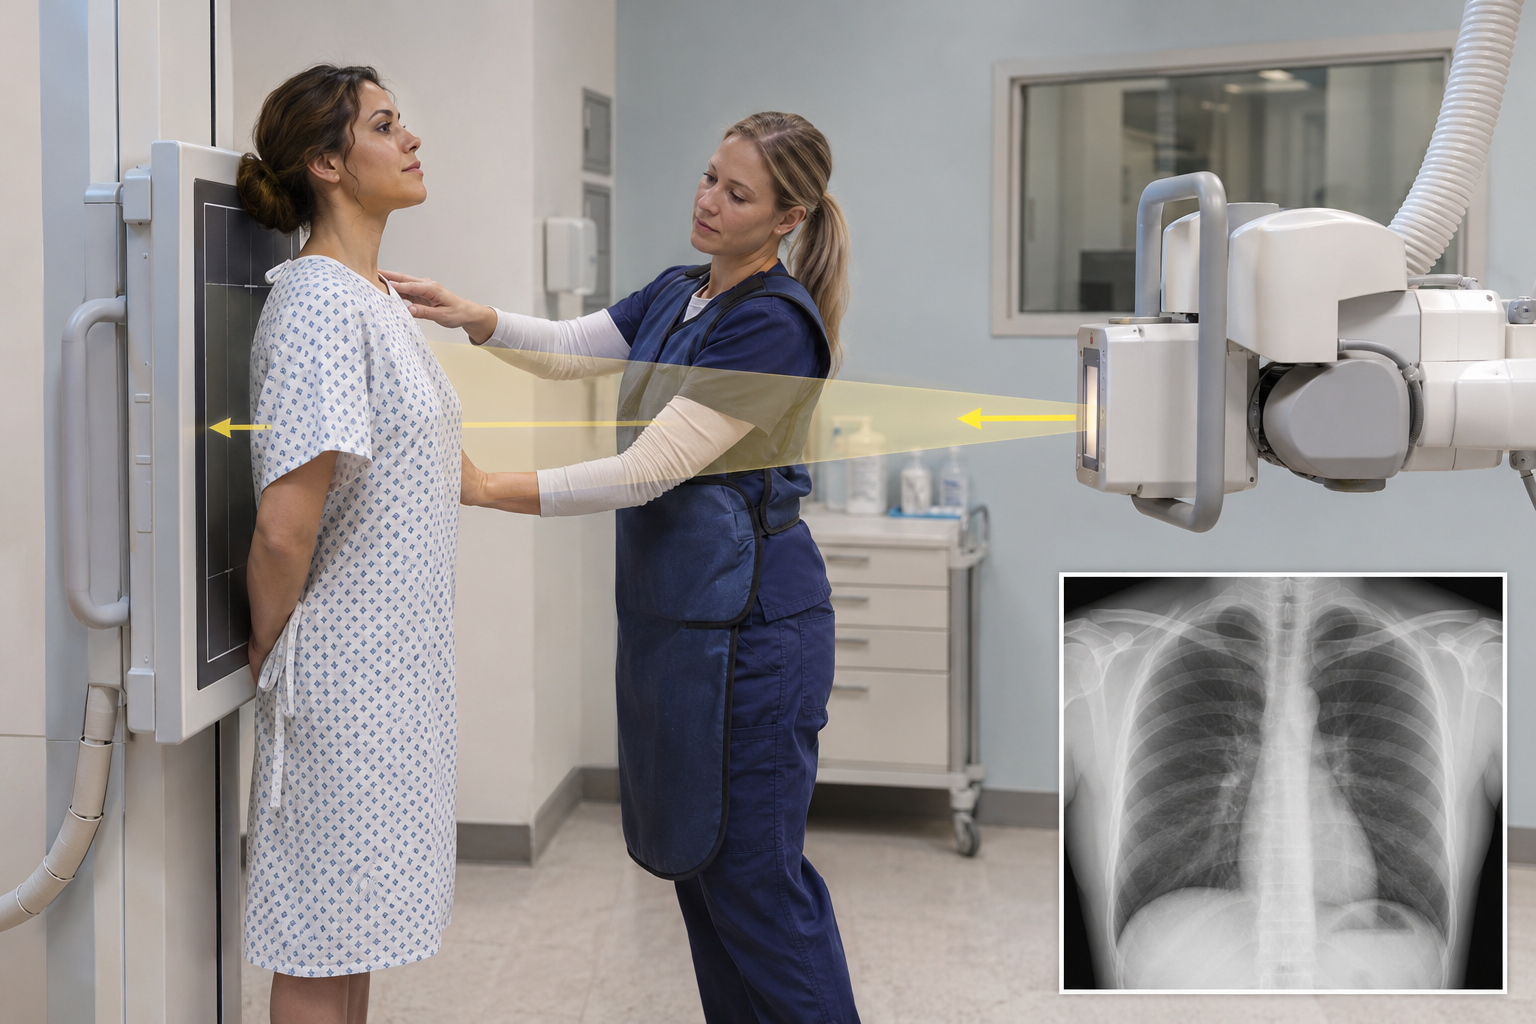
\includegraphics[width=\textwidth,keepaspectratio]{modalities/infographics/x_ray_realistic.png}
\end{center}
\begin{center}\footnotesize Projection radiography records the summed X-ray attenuation along each beam path, so anatomy overlaps and positioning affects visibility. AI-generated illustration; radiograph inset is not a patient study.\end{center}

\section{Overview}
Conventional plain X-ray imaging, also called radiography, produces two-dimensional projection images by passing X-rays through the body to a detector. Dense structures such as bone absorb more X-rays and appear relatively white; air appears dark, while soft tissues appear in shades of grey.

This chapter covers plain projection radiographs of the chest, skeleton, abdomen and urinary tract. A radiograph can reveal the shape of a fracture, show how far joint damage has progressed or suggest the cause of an obstruction. What it reveals depends on the projection, the tissue involved and the stage of disease.

\section{Selected applications of plain radiography}
The numbered entries pair each condition, injury or finding with an example of its appearance. Some appearances have several possible causes. For example, a chest film can show fluid in the pleural space, but identifying blood in that fluid requires additional evidence.

\subsection{Chest X-rays}
\begin{enumerate}[leftmargin=*,itemsep=0.45em,topsep=0.4em]
\item \textbf{Acute respiratory distress syndrome (ARDS).}\par\noindent\textbf{Symptoms:} Acute hypoxemia and respiratory distress prompt bedside chest imaging.\par\noindent\textbf{Clinical Features:} Bilateral opacities, distribution, interval change, and signs of pleural fluid or cardiac enlargement that may suggest another or additional cause.\par\noindent\textbf{Role and sufficiency:} The film supports assessment and monitoring but cannot diagnose ARDS by itself; clinicians combine timing, oxygenation, clinical cause, and exclusion of hydrostatic edema.
\item \textbf{Asbestosis.}\par\noindent\textbf{Symptoms:} Progressive exertional breathlessness or cough in someone with occupational asbestos exposure may prompt imaging.\par\noindent\textbf{Clinical Features:} Basal interstitial markings and pleural plaques; plaques show exposure but do not prove pulmonary fibrosis.\par\noindent\textbf{Role and sufficiency:} Radiography can reveal established disease, but a normal or equivocal film does not exclude early fibrosis. HRCT and exposure history are often needed for characterization.
\item \textbf{Atelectasis.}\par\noindent\textbf{Symptoms:} New breathlessness or low oxygen levels, reduced breath sounds, or postoperative respiratory changes may prompt a chest radiograph; small areas of collapse can also be incidental.\par\noindent\textbf{Clinical Features:} A denser region accompanied by volume loss. Fissure displacement and crowded bronchovascular markings are direct clues; hilar or mediastinal shift toward the affected side, an elevated hemidiaphragm, and compensatory expansion of nearby lung support the interpretation. Air bronchograms may remain visible when bronchi are open, so they do not by themselves exclude collapse.\par\noindent\textbf{Role and sufficiency:} Chest X-ray is usually the initial imaging test and often identifies substantial lobar collapse when these signs are visible. It does not reliably identify the cause; CT or bronchoscopy may be needed when collapse is unexplained, persistent, recurrent, or suspicious for an obstructing lesion. \textbf{Diagnostic performance:} There is no single success percentage for atelectasis across all presentations. Subsegmental or early collapse may be subtle or occult, particularly on a portable single-view study. See the \href{https://www.ncbi.nlm.nih.gov/books/NBK621651/}{NCBI chest radiograph review} and \href{https://pmc.ncbi.nlm.nih.gov/articles/PMC10902601/}{Fleischner Society thoracic imaging glossary}.
\item \textbf{Cardiomegaly.}\par\noindent\textbf{Symptoms:} Breathlessness, edema, or a suspected change in heart size may lead to a chest film.\par\noindent\textbf{Clinical Features:} An enlarged cardiac silhouette, while checking projection, rotation, and inspiration; AP portable views magnify the heart.\par\noindent\textbf{Role and sufficiency:} Radiography can suggest enlargement but cannot measure chamber size or establish its cause. Echocardiography is used when cardiac structure or function needs assessment.
\item \textbf{Congestive heart failure.}\par\noindent\textbf{Symptoms:} Acute breathlessness, shortness of breath when lying flat, or edema may prompt a chest radiograph for pulmonary congestion and alternative diagnoses.\par\noindent\textbf{Clinical Features:} Vascular redistribution, interstitial or alveolar edema, pleural effusions, and cardiac silhouette, interpreted together.\par\noindent\textbf{Role and sufficiency:} The film supports but neither confirms nor excludes heart failure; examination, biomarkers, and echocardiography may be needed.
\item \textbf{Diaphragmatic hernia.}\par\noindent\textbf{Symptoms:} Respiratory distress, chest symptoms, or an incidental thoracic opacity may raise suspicion.\par\noindent\textbf{Clinical Features:} Bowel gas, an air-fluid level, or abdominal viscera above the diaphragm.\par\noindent\textbf{Role and sufficiency:} A radiograph can reveal a conspicuous hernia, but CT or other targeted imaging may be needed to define the defect and contents, especially when the film is equivocal.
\item \textbf{Emphysema.}\par\noindent\textbf{Symptoms:} Chronic breathlessness, cough, or suspected COPD may lead to chest radiography.\par\noindent\textbf{Clinical Features:} Hyperinflation, flattened diaphragms, and increased retrosternal airspace.\par\noindent\textbf{Role and sufficiency:} These are supportive signs, not a measure of airflow obstruction; spirometry establishes COPD, while CT better characterizes emphysema.
\item \textbf{Foreign body aspiration.}\par\noindent\textbf{Symptoms:} Sudden choking or cough, unilateral wheeze, or persistent focal respiratory symptoms—particularly in a child—may prompt imaging.\par\noindent\textbf{Clinical Features:} A radiopaque object, unilateral air trapping, atelectasis, or recurrent focal infection.\par\noindent\textbf{Role and sufficiency:} Many aspirated objects are radiolucent, so a normal film cannot rule out aspiration. Bronchoscopy may be required when clinical suspicion remains high.
\item \textbf{Hemothorax.}\par\noindent\textbf{Symptoms:} Chest trauma with breathlessness, chest pain, or circulatory compromise prompts rapid assessment for pleural blood.\par\noindent\textbf{Clinical Features:} Pleural opacity or layering fluid; a supine film may show only diffuse haziness.\par\noindent\textbf{Role and sufficiency:} X-ray detects larger collections but cannot reliably distinguish blood from other pleural fluid. Ultrasound or CT clarifies uncertain cases and injury extent.
\item \textbf{Lung abscess.}\par\noindent\textbf{Symptoms:} Persistent fever, productive cough, or failure to improve with treatment may prompt imaging for cavitating infection.\par\noindent\textbf{Clinical Features:} A cavity, often with an air-fluid level, within an area of consolidation.\par\noindent\textbf{Role and sufficiency:} The appearance raises suspicion but overlaps with cavitating tumor and tuberculosis; CT and microbiological evaluation help establish cause and extent.
\item \textbf{Lung cancer.}\par\noindent\textbf{Symptoms:} Persistent cough, coughing up blood, unexplained weight loss, or an abnormal screening or prior image may prompt chest radiography.\par\noindent\textbf{Clinical Features:} A new nodule or mass, hilar enlargement, collapse, or pleural effusion.\par\noindent\textbf{Role and sufficiency:} X-ray may detect a lesion but cannot exclude cancer when normal or characterize it definitively. CT and tissue sampling are typically needed for diagnosis and staging.
\item \textbf{Pleural effusion.}\par\noindent\textbf{Symptoms:} Breathlessness, pleuritic discomfort, or suspected fluid accumulation may lead to chest imaging.\par\noindent\textbf{Clinical Features:} Blunting of the costophrenic angle and a meniscus on an upright film; supine fluid may layer diffusely.\par\noindent\textbf{Role and sufficiency:} X-ray can identify moderate or large effusions, but ultrasound detects smaller collections and guides sampling; imaging alone does not determine the cause.
\item \textbf{Pneumonia.}\par\noindent\textbf{Symptoms:} Fever, cough, breathlessness, or low oxygen levels may prompt imaging for a pulmonary infiltrate or complication.\par\noindent\textbf{Clinical Features:} Focal or multifocal air-space opacity, air bronchograms, and pleural fluid, correlated with symptoms and prior studies.\par\noindent\textbf{Role and sufficiency:} Chest radiography is commonly an initial test, but early infection or dehydration may produce a nondiagnostic film. It cannot identify the organism; CT is reserved for selected unresolved or complicated cases.
\item \textbf{Pneumothorax.}\par\noindent\textbf{Symptoms:} Sudden pleuritic pain, breathlessness, trauma, or deterioration after a procedure raises concern.\par\noindent\textbf{Clinical Features:} A visceral pleural line with no peripheral lung markings; assess for mediastinal shift and size.\par\noindent\textbf{Role and sufficiency:} An upright film can confirm a visible pneumothorax, but small or supine cases may be missed. Bedside ultrasound or CT may be needed when suspicion remains; tension physiology is a clinical emergency.
\item \textbf{Pulmonary edema.}\par\noindent\textbf{Symptoms:} Acute breathlessness or hypoxemia may prompt imaging for fluid-related lung changes.\par\noindent\textbf{Clinical Features:} Vascular redistribution, septal lines, bilateral perihilar or diffuse opacities, and pleural effusions.\par\noindent\textbf{Role and sufficiency:} The pattern supports edema but is not specific for a cardiac cause and can lag behind clinical change; cardiac and clinical assessment determine the mechanism.
\item \textbf{Pulmonary fibrosis.}\par\noindent\textbf{Symptoms:} Gradually worsening exertional breathlessness or persistent dry cough may prompt evaluation for chronic interstitial disease.\par\noindent\textbf{Clinical Features:} Reticular opacities, reduced lung volume, and, in advanced disease, basal or peripheral predominance.\par\noindent\textbf{Role and sufficiency:} Radiography may suggest established fibrosis but can be normal early and cannot reliably define pattern or cause. HRCT is generally required for detailed characterization.
\item \textbf{Pulmonary tuberculosis.}\par\noindent\textbf{Symptoms:} Persistent cough, fever, night sweats, weight loss, coughing up blood, or relevant exposure may prompt chest imaging.\par\noindent\textbf{Clinical Features:} Upper-lung opacity, cavitation, nodules, or other patterns, while recognizing that distribution varies with immune status and disease stage.\par\noindent\textbf{Role and sufficiency:} X-ray can raise suspicion and assess extent but cannot confirm active TB or exclude it when normal. Sputum testing and clinical assessment are required.
\item \textbf{Sarcoidosis.}\par\noindent\textbf{Symptoms:} Cough, breathlessness, systemic symptoms, or incidental hilar enlargement may prompt evaluation.\par\noindent\textbf{Clinical Features:} Bilateral hilar or mediastinal lymph-node enlargement and interstitial lung changes.\par\noindent\textbf{Role and sufficiency:} The radiograph helps identify and stage thoracic involvement, but the pattern is not specific; diagnosis depends on clinical context and sometimes tissue sampling.
\item \textbf{Silicosis.}\par\noindent\textbf{Symptoms:} A history of silica exposure with chronic cough or breathlessness may lead to occupational lung assessment.\par\noindent\textbf{Clinical Features:} Small rounded upper-lung nodules, conglomerate opacities, and possible eggshell calcification of hilar nodes.\par\noindent\textbf{Role and sufficiency:} Radiography can show established disease but may miss early abnormalities; exposure history and, when needed, HRCT help resolve equivocal films.
\end{enumerate}

\subsection{Bone X-rays}
\begin{enumerate}[leftmargin=*,itemsep=0.45em,topsep=0.4em]
\item \textbf{Achondroplasia.}\par\noindent\textbf{Symptoms:} Disproportionate short stature or limb bowing prompts skeletal survey and growth assessment.\par\noindent\textbf{Clinical Features:} Rhizomelic shortening, characteristic metaphyseal and pelvic shape, and spinal canal or thoracolumbar changes.\par\noindent\textbf{Role and sufficiency:} Radiographs can support the skeletal diagnosis; clinical genetics and, when needed, molecular testing establish the subtype and assess complications.
\item \textbf{Aneurysmal bone cyst.}\par\noindent\textbf{Symptoms:} Focal bone pain, swelling, or a pathologic fracture in a young person may prompt imaging.\par\noindent\textbf{Clinical Features:} An expansile, eccentric lucent lesion with a thin shell of bone.\par\noindent\textbf{Role and sufficiency:} X-ray detects and localizes many lesions, but MRI/CT defines extent and fluid levels; tissue diagnosis may be required because other tumors can look similar.
\item \textbf{Avascular necrosis.}\par\noindent\textbf{Symptoms:} Persistent joint pain, especially with risk factors such as corticosteroid exposure or prior trauma, may prompt imaging.\par\noindent\textbf{Clinical Features:} Sclerosis, a subchondral crescent, flattening, or collapse.\par\noindent\textbf{Role and sufficiency:} Radiographs show established disease and collapse; early osteonecrosis may be occult, so MRI is preferred when suspicion remains despite normal films.
\item \textbf{Avulsion fracture.}\par\noindent\textbf{Symptoms:} Sudden pain after forceful muscle contraction or ligament injury prompts targeted views.\par\noindent\textbf{Clinical Features:} A small displaced fragment at a tendon or ligament attachment and its donor site.\par\noindent\textbf{Role and sufficiency:} Radiography usually identifies a visible fragment and alignment; MRI or CT may be needed for occult injury or operative planning.
\item \textbf{Bone metastases.}\par\noindent\textbf{Symptoms:} Focal bone pain, a suspected pathologic fracture, or known cancer may prompt imaging of a symptomatic site.\par\noindent\textbf{Clinical Features:} Destructive lytic or sclerotic lesions, cortical loss, and fracture.\par\noindent\textbf{Role and sufficiency:} A film can show established lesions but may miss early marrow disease; it cannot stage the skeleton, and MRI, CT, PET, or bone scintigraphy may be selected for extent.
\item \textbf{Chondrosarcoma.}\par\noindent\textbf{Symptoms:} Persistent focal bone pain or an enlarging mass may prompt imaging of a cartilage lesion.\par\noindent\textbf{Clinical Features:} Rings-and-arcs chondroid matrix, endosteal scalloping, cortical destruction, or soft-tissue extension.\par\noindent\textbf{Role and sufficiency:} Radiography characterizes matrix and aggressiveness but cannot reliably grade the tumor; MRI defines local extent and specialist-led biopsy establishes histology.
\item \textbf{Comminuted fracture.}\par\noindent\textbf{Symptoms:} Acute pain, deformity, or loss of function after trauma leads to initial fracture imaging.\par\noindent\textbf{Clinical Features:} Multiple fragments, displacement, angulation, and joint extension on at least two views.\par\noindent\textbf{Role and sufficiency:} Radiographs usually establish the fracture pattern; CT is added when complex articular anatomy or operative planning requires more detail.
\item \textbf{Ewing sarcoma.}\par\noindent\textbf{Symptoms:} Persistent focal bone pain, swelling, or unexplained fever in a child or young adult prompts investigation.\par\noindent\textbf{Clinical Features:} An aggressive permeative lesion and layered periosteal reaction; neither sign is unique to Ewing sarcoma.\par\noindent\textbf{Role and sufficiency:} X-ray is an initial clue, not a definitive diagnosis. MRI defines extent and biopsy is required; referral should precede biopsy.
\item \textbf{Fibrous dysplasia.}\par\noindent\textbf{Symptoms:} Bone pain, deformity, or an incidental lesion may lead to radiography.\par\noindent\textbf{Clinical Features:} A ground-glass matrix, smooth expansion, and a rind of sclerosis in the involved bone.\par\noindent\textbf{Role and sufficiency:} A characteristic film may be sufficient for a typical lesion, but atypical pain, aggressive change, or uncertain appearance warrants CT/MRI and specialist assessment.
\item \textbf{Giant cell tumor.}\par\noindent\textbf{Symptoms:} Pain and swelling near a joint in a skeletally mature young adult may prompt imaging.\par\noindent\textbf{Clinical Features:} An eccentric expansile lytic lesion extending to the subarticular bone, usually without a sclerotic margin.\par\noindent\textbf{Role and sufficiency:} X-ray suggests the pattern; MRI/CT evaluates cortical and soft-tissue extent, and histology is needed before treatment.
\item \textbf{Greenstick fracture.}\par\noindent\textbf{Symptoms:} A child with limb pain or deformity after a fall needs targeted radiographs.\par\noindent\textbf{Clinical Features:} One cortex breaks while the opposite cortex bends, with possible angulation.\par\noindent\textbf{Role and sufficiency:} Two-view radiographs usually identify the fracture and guide alignment assessment; additional views may be needed if the joint or growth plate is involved.
\item \textbf{Impacted fracture.}\par\noindent\textbf{Symptoms:} Pain and reduced movement after a fall or axial load prompt fracture imaging.\par\noindent\textbf{Clinical Features:} Trabecular impaction, shortening, or a band of sclerosis at the fracture site.\par\noindent\textbf{Role and sufficiency:} X-ray may show an impacted fracture, but nondisplaced injuries can be subtle; CT or MRI follows when focal symptoms persist despite negative films.
\item \textbf{Oblique fracture.}\par\noindent\textbf{Symptoms:} Localized pain, swelling, or inability to use a limb after trauma prompts radiographs.\par\noindent\textbf{Clinical Features:} A fracture line crossing the bone diagonally, plus displacement and rotation on orthogonal views.\par\noindent\textbf{Role and sufficiency:} Radiographs usually establish the pattern; CT is useful if the fracture extends into a complex joint surface.
\item \textbf{Osteochondroma.}\par\noindent\textbf{Symptoms:} A palpable bony lump, mechanical irritation, or incidental imaging finding may prompt assessment.\par\noindent\textbf{Clinical Features:} A metaphyseal exostosis with cortex and medullary canal continuous with the parent bone.\par\noindent\textbf{Role and sufficiency:} A typical film can establish the characteristic appearance; MRI is appropriate for new pain, growth after skeletal maturity, or suspected cartilage-cap complications.
\item \textbf{Osteogenesis imperfecta.}\par\noindent\textbf{Symptoms:} Recurrent fractures, bone deformity, or suspected fragility in a child prompts skeletal imaging.\par\noindent\textbf{Clinical Features:} Fractures of different ages, bowing, osteopenia, and vertebral compression.\par\noindent\textbf{Role and sufficiency:} Radiographs document skeletal complications but do not establish the genetic diagnosis; clinical and genetic assessment is required.
\item \textbf{Osteomalacia.}\par\noindent\textbf{Symptoms:} Diffuse bone pain, muscle weakness, or suspected insufficiency fracture may prompt imaging.\par\noindent\textbf{Clinical Features:} Looser zones (pseudofractures), often in characteristic sites, and generalized demineralization.\par\noindent\textbf{Role and sufficiency:} Films may reveal advanced disease but can be normal early; biochemical testing and clinical context are needed to identify the cause.
\item \textbf{Osteomyelitis.}\par\noindent\textbf{Symptoms:} Focal bone pain, fever, or a nearby wound raises concern for infection.\par\noindent\textbf{Clinical Features:} Periosteal reaction, cortical destruction, or soft-tissue swelling, recognizing that changes may lag symptoms.\par\noindent\textbf{Role and sufficiency:} X-ray is useful as a baseline and for established bone damage, but early films are often normal; MRI and microbiological sampling may be needed.
\item \textbf{Osteopetrosis.}\par\noindent\textbf{Symptoms:} Recurrent fractures, bone pain, or incidental dense bones may prompt skeletal evaluation.\par\noindent\textbf{Clinical Features:} Diffuse increased density and characteristic modeling abnormalities.\par\noindent\textbf{Role and sufficiency:} The radiographic pattern strongly suggests osteopetrosis, but clinical, hematologic, and genetic evaluation defines type and complications.
\item \textbf{Osteosarcoma.}\par\noindent\textbf{Symptoms:} Persistent focal bone pain or swelling, often near the knee in an adolescent, warrants radiography.\par\noindent\textbf{Clinical Features:} An aggressive mixed lytic-sclerotic lesion, cortical destruction, and possible sunburst periosteal reaction or soft-tissue mineralization.\par\noindent\textbf{Role and sufficiency:} X-ray raises urgent suspicion but cannot confirm histology or local extent; MRI and specialist biopsy are required.
\item \textbf{Paget disease of bone.}\par\noindent\textbf{Symptoms:} Bone pain, deformity, hearing symptoms, or an incidental alkaline-phosphatase elevation may prompt targeted imaging.\par\noindent\textbf{Clinical Features:} Bone expansion, cortical thickening, coarsened trabeculae, and mixed lytic-sclerotic phases.\par\noindent\textbf{Role and sufficiency:} Typical radiographs often establish the pattern in the imaged bone; biochemical and clinical correlation assess activity and complications.
\item \textbf{Rickets.}\par\noindent\textbf{Symptoms:} A child with growth delay, limb bowing, or bone pain may need radiographs of the wrist or knee.\par\noindent\textbf{Clinical Features:} Widened growth plates with metaphyseal cupping, fraying, and splaying.\par\noindent\textbf{Role and sufficiency:} The film can demonstrate established rickets, but laboratory tests are required to determine the nutritional, renal, or genetic cause.
\item \textbf{Spiral fracture.}\par\noindent\textbf{Symptoms:} Pain and swelling after a twisting injury prompt radiographs of the affected bone and adjacent joints.\par\noindent\textbf{Clinical Features:} A helical fracture line and any rotation or displacement on orthogonal views.\par\noindent\textbf{Role and sufficiency:} Radiographs usually identify a visible fracture; subtle nondisplaced injuries may require repeat films or CT/MRI if symptoms persist.
\item \textbf{Stress fracture.}\par\noindent\textbf{Symptoms:} Gradually increasing focal pain with repetitive loading or a sudden training increase prompts imaging.\par\noindent\textbf{Clinical Features:} Periosteal reaction, cortical thickening, or a fracture line; early radiographs can be normal.\par\noindent\textbf{Role and sufficiency:} X-ray is a common initial test but does not exclude an early stress injury. MRI is preferred when suspicion remains or early confirmation matters.
\item \textbf{Torus fracture.}\par\noindent\textbf{Symptoms:} A child with localized pain after a fall onto an outstretched hand commonly receives wrist radiographs.\par\noindent\textbf{Clinical Features:} Buckling of the cortex without a complete break.\par\noindent\textbf{Role and sufficiency:} Two-view radiographs usually suffice to diagnose this stable fracture and guide treatment; check adjacent growth plates and joints.
\item \textbf{Transverse fracture.}\par\noindent\textbf{Symptoms:} Focal pain, swelling, or deformity following direct impact prompts imaging.\par\noindent\textbf{Clinical Features:} A fracture line perpendicular to the bone's long axis, with displacement, angulation, and joint extension.\par\noindent\textbf{Role and sufficiency:} Radiographs usually establish the pattern; CT may be needed for complex articular fractures or surgical planning.
\item \textbf{Unicameral bone cyst.}\par\noindent\textbf{Symptoms:} A pathologic fracture or incidental long-bone lesion in a child or adolescent may prompt imaging.\par\noindent\textbf{Clinical Features:} A central, well-defined metaphyseal lucency with cortical thinning; a fallen fragment may appear after fracture.\par\noindent\textbf{Role and sufficiency:} X-ray often suggests a typical cyst, but MRI/CT or specialist review may be needed when the lesion is atypical or aggressive.
\end{enumerate}

\subsection{Joint X-rays}
\begin{enumerate}[leftmargin=*,itemsep=0.45em,topsep=0.4em]
\item \textbf{Ankylosing spondylitis.}\par\noindent\textbf{Symptoms:} Chronic inflammatory back or buttock pain and stiffness may prompt sacroiliac imaging.\par\noindent\textbf{Clinical Features:} Sacroiliac erosions, sclerosis, joint-space change, and fusion in advanced disease.\par\noindent\textbf{Role and sufficiency:} Radiographs detect established structural disease but may be normal early; MRI can show active inflammation before bony changes.
\item \textbf{Blount disease.}\par\noindent\textbf{Symptoms:} Progressive bowing of a child's legs, especially around the knee, prompts standing alignment views.\par\noindent\textbf{Clinical Features:} Varus angulation and abnormal medial proximal tibial metaphysis.\par\noindent\textbf{Role and sufficiency:} Radiographs are central to diagnosis and severity assessment when properly positioned; clinical growth and alignment assessment guide management.
\item \textbf{Calcific tendinitis.}\par\noindent\textbf{Symptoms:} Acute shoulder pain or restricted movement may lead to imaging for tendon calcification and competing bone causes.\par\noindent\textbf{Clinical Features:} A dense deposit near the rotator cuff insertion.\par\noindent\textbf{Role and sufficiency:} X-ray can show the deposit, but it may be incidental and does not prove it causes the pain; ultrasound evaluates tendon and deposit shape.
\item \textbf{Calcium pyrophosphate deposition (CPPD).}\par\noindent\textbf{Symptoms:} Acute joint swelling or chronic joint pain may prompt imaging for cartilage calcification or an alternative diagnosis.\par\noindent\textbf{Clinical Features:} Chondrocalcinosis and an atypical osteoarthritis distribution.\par\noindent\textbf{Role and sufficiency:} The finding supports CPP deposition but can be incidental; X-ray cannot confirm an acute crystal attack, which requires clinical assessment and sometimes synovial-fluid analysis.
\item \textbf{Charcot arthropathy.}\par\noindent\textbf{Symptoms:} A warm, swollen, relatively painless foot in a patient with neuropathy raises concern for joint destruction.\par\noindent\textbf{Clinical Features:} Fragmentation, subluxation, disorganization, and progressive collapse.\par\noindent\textbf{Role and sufficiency:} Radiographs show established structural damage and provide a baseline; early disease may be occult, so MRI is considered when suspicion remains.
\item \textbf{Developmental hip dysplasia.}\par\noindent\textbf{Symptoms:} Abnormal hip examination or later presentation with limited motion or gait asymmetry prompts age-appropriate imaging.\par\noindent\textbf{Clinical Features:} Acetabular shallowing and femoral-head position once the ossification center is visible.\par\noindent\textbf{Role and sufficiency:} Pelvic radiographs are useful after sufficient ossification; ultrasound is preferred in young infants whose femoral heads remain largely cartilaginous.
\item \textbf{Gout.}\par\noindent\textbf{Symptoms:} Recurrent joint attacks or chronic deformity may prompt assessment for established erosive disease.\par\noindent\textbf{Clinical Features:} Well-defined juxta-articular erosions with overhanging edges and preserved joint space until late.\par\noindent\textbf{Role and sufficiency:} X-ray can support longstanding gout but is often normal early and cannot confirm an acute flare; crystal analysis or other targeted imaging may be needed.
\item \textbf{Joint dislocation.}\par\noindent\textbf{Symptoms:} Deformity, severe pain, or loss of function after injury prompts immediate joint imaging.\par\noindent\textbf{Clinical Features:} Loss of normal articular alignment, associated fracture, and post-reduction position.\par\noindent\textbf{Role and sufficiency:} Radiographs usually establish a visible dislocation and verify reduction; additional views or CT may be required for complex joints or associated fractures.
\item \textbf{Joint subluxation.}\par\noindent\textbf{Symptoms:} Pain, instability, or deformity after injury may raise concern for partial displacement.\par\noindent\textbf{Clinical Features:} Incomplete loss of congruity between articular surfaces, compared with the normal relationship.\par\noindent\textbf{Role and sufficiency:} X-ray can demonstrate subluxation if positioning captures it; dynamic instability or soft-tissue injury may require examination, stress views, or MRI.
\item \textbf{Legg--Calv\'e--Perthes disease.}\par\noindent\textbf{Symptoms:} A child with a limp, hip or referred knee pain, and limited hip motion may need pelvic radiographs.\par\noindent\textbf{Clinical Features:} Femoral-head sclerosis, flattening, fragmentation, and later reossification.\par\noindent\textbf{Role and sufficiency:} X-ray is the initial study and stages visible disease, but early films can be normal; MRI is useful when clinical suspicion remains high.
\item \textbf{Osteoarthritis.}\par\noindent\textbf{Symptoms:} Activity-related joint pain, stiffness, or reduced range of motion may prompt assessment of structural change.\par\noindent\textbf{Clinical Features:} Nonuniform joint-space narrowing, osteophytes, subchondral sclerosis, and cysts.\par\noindent\textbf{Role and sufficiency:} Radiographs commonly support diagnosis and grade structural disease, but the degree of change does not by itself measure pain or function.
\item \textbf{Psoriatic arthritis.}\par\noindent\textbf{Symptoms:} Persistent joint pain or swelling in a person with psoriasis may prompt imaging for erosive or proliferative change.\par\noindent\textbf{Clinical Features:} Erosions with new bone formation, pencil-in-cup deformity, or asymmetric involvement in established disease.\par\noindent\textbf{Role and sufficiency:} X-ray documents chronic damage but may be normal early; clinical assessment and ultrasound or MRI can evaluate active inflammation.
\item \textbf{Rheumatoid arthritis.}\par\noindent\textbf{Symptoms:} Persistent symmetric small-joint swelling and stiffness may prompt baseline or interval imaging.\par\noindent\textbf{Clinical Features:} Marginal erosions, periarticular osteopenia, and uniform joint-space loss.\par\noindent\textbf{Role and sufficiency:} Films document structural damage but can miss early synovitis; examination, laboratory findings, and sometimes ultrasound/MRI establish activity and support diagnosis.
\item \textbf{Septic arthritis.}\par\noindent\textbf{Symptoms:} Acute painful swollen joint with fever or inability to bear weight prompts imaging for baseline damage and alternative diagnoses.\par\noindent\textbf{Clinical Features:} Early films may show only soft-tissue swelling or effusion; joint-space loss and bone destruction are late.\par\noindent\textbf{Role and sufficiency:} A normal X-ray does not exclude infection. Urgent aspiration and culture are central; imaging must not delay treatment when suspicion is high.
\item \textbf{Slipped capital femoral epiphysis.}\par\noindent\textbf{Symptoms:} An adolescent with hip, groin, thigh, or referred knee pain and limited internal rotation needs urgent imaging.\par\noindent\textbf{Clinical Features:} Posterior-inferior displacement of the epiphysis relative to the femoral neck on appropriate views.\par\noindent\textbf{Role and sufficiency:} Radiographs usually establish a visible slip; if suspicion remains despite normal films, urgent specialist assessment and MRI may be appropriate. Avoid forceful positioning.
\end{enumerate}

\subsection{Spine X-rays}
\begin{enumerate}[leftmargin=*,itemsep=0.45em,topsep=0.4em]
\item \textbf{Degenerative disc disease.}\par\noindent\textbf{Symptoms:} Chronic axial back or neck pain may prompt films when structural alignment or degeneration is relevant.\par\noindent\textbf{Clinical Features:} Disc-space narrowing, endplate sclerosis, and osteophytes.\par\noindent\textbf{Role and sufficiency:} X-rays show chronic bony change but do not identify the pain generator or assess discs and nerves well; MRI is used for neurologic symptoms or suspected infection/tumor.
\item \textbf{Diffuse idiopathic skeletal hyperostosis (DISH).}\par\noindent\textbf{Symptoms:} Stiffness, reduced spinal motion, or an incidental finding may prompt imaging.\par\noindent\textbf{Clinical Features:} Flowing anterolateral ossification across contiguous vertebrae with relative preservation of disc height.\par\noindent\textbf{Role and sufficiency:} Radiographs usually show established DISH; clinical context and additional imaging distinguish it from inflammatory disease or other causes of ossification.
\item \textbf{Sacroiliitis.}\par\noindent\textbf{Symptoms:} Inflammatory buttock or low-back pain may prompt evaluation of the sacroiliac joints.\par\noindent\textbf{Clinical Features:} Erosions, sclerosis, joint-space alteration, or ankylosis.\par\noindent\textbf{Role and sufficiency:} X-ray detects established structural change but can miss early active inflammation; MRI is preferred when early sacroiliitis is suspected.
\item \textbf{Scheuermann disease.}\par\noindent\textbf{Symptoms:} Adolescent back pain or a fixed thoracic kyphosis prompts standing spine views.\par\noindent\textbf{Clinical Features:} Anterior wedging of multiple consecutive vertebrae with endplate irregularity and Schmorl nodes.\par\noindent\textbf{Role and sufficiency:} Radiographs usually establish the structural pattern; clinical exam distinguishes it from postural kyphosis and other causes.
\item \textbf{Scoliosis.}\par\noindent\textbf{Symptoms:} Visible trunk asymmetry, shoulder or pelvic imbalance, or a screening finding may prompt standing spine imaging.\par\noindent\textbf{Clinical Features:} Coronal curvature, vertebral rotation, curve location, and skeletal maturity.\par\noindent\textbf{Role and sufficiency:} A properly positioned standing series measures the curve for monitoring; it does not identify every cause, and MRI is considered for atypical features or neurologic findings.
\item \textbf{Spinal tuberculosis.}\par\noindent\textbf{Symptoms:} Persistent back pain with fever, weight loss, TB exposure, or neurologic symptoms may prompt spinal evaluation.\par\noindent\textbf{Clinical Features:} Vertebral endplate destruction, disc-space narrowing, collapse, or paraspinal soft-tissue change; these can be late and are nonspecific.\par\noindent\textbf{Role and sufficiency:} X-ray cannot exclude early infection or confirm tuberculosis. MRI and microbiological or tissue testing are usually required.
\item \textbf{Spondylolisthesis.}\par\noindent\textbf{Symptoms:} Mechanical back pain, deformity, or leg symptoms may prompt alignment imaging.\par\noindent\textbf{Clinical Features:} Translation of one vertebra relative to another, level, and severity; standing views may reveal load-related slippage.\par\noindent\textbf{Role and sufficiency:} Radiographs show alignment but do not assess nerve compression; MRI is added for persistent radicular or neurologic symptoms.
\item \textbf{Spondylolysis.}\par\noindent\textbf{Symptoms:} Focal extension-related low-back pain, particularly in an athlete, may prompt evaluation for a pars defect.\par\noindent\textbf{Clinical Features:} A pars interarticularis defect, often at L5, and any associated vertebral slip.\par\noindent\textbf{Role and sufficiency:} X-rays may identify established defects but can miss early stress injury; MRI or CT may be needed when symptoms persist or precise bony definition is needed.
\item \textbf{Spondylosis.}\par\noindent\textbf{Symptoms:} Chronic neck or back pain, stiffness, or suspected degenerative alignment change may prompt radiography.\par\noindent\textbf{Clinical Features:} Osteophytes, facet degeneration, disc-space narrowing, and alignment.\par\noindent\textbf{Role and sufficiency:} X-rays show common age-related structural changes but cannot prove they cause symptoms or evaluate the spinal cord and nerve roots.
\item \textbf{Thoracic hyperkyphosis.}\par\noindent\textbf{Symptoms:} A visible rounded back, height loss, or progressive posture change may prompt a lateral standing view.\par\noindent\textbf{Clinical Features:} Increased thoracic curvature and vertebral wedging or compression fractures.\par\noindent\textbf{Role and sufficiency:} Radiographs quantify the curve and show bony contributors; clinical assessment is needed to distinguish postural, developmental, and fracture-related causes.
\item \textbf{Vertebral compression fracture.}\par\noindent\textbf{Symptoms:} Sudden back pain after minor trauma or height loss in a person at fracture risk prompts spine imaging.\par\noindent\textbf{Clinical Features:} Vertebral height loss, endplate deformity, and alignment.\par\noindent\textbf{Role and sufficiency:} X-ray can show a collapsed vertebra but may not determine whether it is acute or benign versus malignant; MRI, CT, or clinical history may be needed.
\end{enumerate}

\subsection{Abdominal X-rays}
\begin{enumerate}[leftmargin=*,itemsep=0.45em,topsep=0.4em]
\item \textbf{Cecal volvulus.}\par\noindent\textbf{Symptoms:} Acute abdominal swelling, pain, and vomiting raise concern for bowel obstruction.\par\noindent\textbf{Clinical Features:} A markedly dilated, displaced cecum and paucity of distal gas.\par\noindent\textbf{Role and sufficiency:} The film may suggest volvulus, but CT is generally needed to confirm the twist, identify ischemia, and guide urgent management.
\item \textbf{Chronic calcific pancreatitis.}\par\noindent\textbf{Symptoms:} Chronic upper abdominal pain or suspected longstanding pancreatitis may lead to abdominal imaging.\par\noindent\textbf{Clinical Features:} Coarse pancreatic calcifications in the expected upper abdominal distribution.\par\noindent\textbf{Role and sufficiency:} Calcifications support chronic disease but are absent in many cases and are not specific; CT/MRI and clinical assessment characterize the pancreas.
\item \textbf{Duodenal atresia.}\par\noindent\textbf{Symptoms:} A newborn with early bilious vomiting prompts urgent evaluation for proximal obstruction.\par\noindent\textbf{Clinical Features:} The double-bubble pattern and amount of distal bowel gas.\par\noindent\textbf{Role and sufficiency:} The pattern strongly suggests duodenal obstruction but is not unique to atresia; pediatric and surgical assessment plus targeted imaging establish anatomy.
\item \textbf{Gastrointestinal perforation.}\par\noindent\textbf{Symptoms:} Sudden severe abdominal pain, guarding, or deterioration may prompt a rapid search for free air.\par\noindent\textbf{Clinical Features:} Subdiaphragmatic or other outside the bowel air on appropriate views.\par\noindent\textbf{Role and sufficiency:} Visible free air is an urgent clue, but its absence does not rule out perforation; CT is more sensitive and may locate the source when the patient is stable.
\item \textbf{Ingested foreign body.}\par\noindent\textbf{Symptoms:} A witnessed ingestion, choking episode, or unexplained pain may prompt imaging, especially in a child.\par\noindent\textbf{Clinical Features:} The location, number, and orientation of radiopaque objects; assess for free air or obstruction.\par\noindent\textbf{Role and sufficiency:} X-ray works for radiopaque objects but can miss food, plastic, and other radiolucent material; endoscopy or CT may be needed depending on symptoms and object type.
\item \textbf{Jejunoileal atresia.}\par\noindent\textbf{Symptoms:} A newborn with bilious vomiting and failure to pass stool may need urgent obstruction imaging.\par\noindent\textbf{Clinical Features:} Dilated proximal bowel loops with little or no distal gas.\par\noindent\textbf{Role and sufficiency:} The film localizes an obstructive pattern but does not always define the number or level of atresias; surgical assessment and additional imaging may be required.
\item \textbf{Large bowel obstruction.}\par\noindent\textbf{Symptoms:} Progressive abdominal swelling, constipation, vomiting, or inability to pass flatus may prompt imaging.\par\noindent\textbf{Clinical Features:} Colonic widening, the distribution of gas, and possible volvulus pattern.\par\noindent\textbf{Role and sufficiency:} Radiography can rapidly suggest obstruction, but CT is generally needed to locate the transition, cause, and complications.
\item \textbf{Meconium ileus.}\par\noindent\textbf{Symptoms:} A newborn with abdominal swelling and delayed passage of meconium prompts evaluation for distal small-bowel obstruction.\par\noindent\textbf{Clinical Features:} Dilated loops and a granular or soap-bubble appearance in the right lower abdomen.\par\noindent\textbf{Role and sufficiency:} The pattern is suggestive but not diagnostic of cystic fibrosis; contrast enema and clinical/genetic evaluation may be needed.
\item \textbf{Necrotizing enterocolitis.}\par\noindent\textbf{Symptoms:} A premature or critically ill infant with feeding intolerance, swelling, bloody stool, or systemic instability needs prompt serial imaging.\par\noindent\textbf{Clinical Features:} Pneumatosis intestinalis, portal venous gas, bowel widening, and free air.\par\noindent\textbf{Role and sufficiency:} Radiographs are central for detecting progression and perforation, but early films may be nonspecific; findings must be interpreted with the infant's clinical course.
\item \textbf{Paralytic ileus.}\par\noindent\textbf{Symptoms:} Distension, nausea, vomiting, or absent bowel function after surgery or severe illness may prompt imaging.\par\noindent\textbf{Clinical Features:} Diffuse bowel widening involving small and large bowel without a clear transition point.\par\noindent\textbf{Role and sufficiency:} The pattern supports ileus but can overlap with mechanical obstruction; CT is used when symptoms or film findings leave that distinction uncertain.
\item \textbf{Sigmoid volvulus.}\par\noindent\textbf{Symptoms:} Marked swelling, pain, and constipation—often in an older or institutionalized patient—raise concern for volvulus.\par\noindent\textbf{Clinical Features:} A large inverted U or coffee-bean loop with its apex directed upward.\par\noindent\textbf{Role and sufficiency:} The sign can strongly suggest sigmoid volvulus, but CT or contrast enema may confirm the level and assess complications; urgent management depends on clinical stability.
\item \textbf{Small bowel obstruction.}\par\noindent\textbf{Symptoms:} Colicky abdominal pain, vomiting, swelling, and reduced stool or flatus may prompt initial imaging.\par\noindent\textbf{Clinical Features:} Dilated small-bowel loops, step-ladder air-fluid levels, and relative paucity of colonic gas.\par\noindent\textbf{Role and sufficiency:} The film may support obstruction but often cannot identify its cause or complications; CT is usually preferred in adults with acute symptoms.
\item \textbf{Toxic megacolon.}\par\noindent\textbf{Symptoms:} Severe colitis with fever, tachycardia, abdominal swelling, or systemic toxicity prompts urgent imaging.\par\noindent\textbf{Clinical Features:} Marked colonic widening, loss of haustra, and signs of perforation.\par\noindent\textbf{Role and sufficiency:} Serial radiographs can monitor colonic diameter, but diagnosis requires clinical toxicity plus imaging and should trigger urgent specialist management.
\end{enumerate}

\subsection{Kidney, ureter and bladder X-rays (KUB)}
\begin{enumerate}[leftmargin=*,itemsep=0.45em,topsep=0.4em]
\item \textbf{Bladder stones.}\par\noindent\textbf{Symptoms:} Urinary frequency, painful voiding, recurrent infection, or a known radiopaque stone may prompt imaging.\par\noindent\textbf{Clinical Features:} A calcific opacity within the bladder region, while considering pelvic phleboliths and other calcifications.\par\noindent\textbf{Role and sufficiency:} KUB may show a radiopaque stone but does not reliably identify all stones or establish obstruction; ultrasound or CT is often used when symptoms persist or localization is uncertain.
\item \textbf{Kidney stones.}\par\noindent\textbf{Symptoms:} Flank pain or follow-up of a previously identified radiopaque calculus may prompt a KUB image.\par\noindent\textbf{Clinical Features:} A calcific focus projected over the renal outline; stone composition affects visibility.\par\noindent\textbf{Role and sufficiency:} KUB can track selected known stones but misses radiolucent stones, including most uric-acid calculi, and cannot reliably exclude renal colic; ultrasound or noncontrast CT is often needed.
\item \textbf{Nephrocalcinosis.}\par\noindent\textbf{Symptoms:} Metabolic abnormalities, renal dysfunction, or suspected medullary calcification may prompt imaging.\par\noindent\textbf{Clinical Features:} Fine or coarse calcification distributed within the renal parenchyma rather than a single collecting-system stone.\par\noindent\textbf{Role and sufficiency:} A visible pattern supports renal calcification but does not identify its cause; ultrasound/CT and laboratory evaluation help define distribution and etiology.
\item \textbf{Staghorn calculus.}\par\noindent\textbf{Symptoms:} Recurrent urinary infection, flank discomfort, or follow-up of a known branching stone may prompt KUB imaging.\par\noindent\textbf{Clinical Features:} A large branching opacity occupying the renal pelvis and extending into calyces.\par\noindent\textbf{Role and sufficiency:} X-ray can track a radiopaque stone, but CT best defines its extent and associated obstruction; a film cannot assess renal function or infection severity.
\item \textbf{Ureteral stones.}\par\noindent\textbf{Symptoms:} Colicky flank-to-groin pain or follow-up of a known radiopaque ureteral stone may prompt imaging.\par\noindent\textbf{Clinical Features:} A calcification along the expected ureteral course, distinguishing possible phleboliths by location and appearance.\par\noindent\textbf{Role and sufficiency:} A positive KUB may help follow selected stones, but a negative film does not exclude ureterolithiasis; ultrasound or noncontrast CT is more sensitive.
\end{enumerate}

\subsection{Summary}
\begin{center}
\begin{tabular}{@{}lr@{}}
\toprule
\textbf{Anatomical region} & \textbf{Entries} \\
\midrule
Abdomen & 13 \\
Bones & 26 \\
Chest & 19 \\
Joints & 15 \\
Kidney, ureter and bladder & 5 \\
Spine & 11 \\
\midrule
\midrule
\textbf{Total} & \textbf{89} \\
\bottomrule
\end{tabular}
\end{center}

The 89 entries include diseases, fracture patterns and imaging findings. Some overlap: a staghorn calculus, for example, is a subtype of kidney stone. For a dataset, record the visible sign separately from the confirmed diagnosis, particularly when several diseases can produce the same appearance.

\paragraph{Selected references.}
The \href{https://archive.cdc.gov/www_atsdr_cdc_gov/csem/asbestos/clinical_assessment-tests.html}{ATSDR asbestos assessment} describes the distinction between pulmonary fibrosis and pleural plaques.
The \href{https://ard.bmj.com/content/83/6/752}{EULAR imaging recommendations} cover crystal deposition.
The American College of Radiology provides criteria for \href{https://acsearch.acr.org/docs/3094201/Narrative/}{bone and joint infection},
\href{https://acsearch.acr.org/docs/69420/Narrative/}{osteonecrosis},
\href{https://acsearch.acr.org/docs/69437/Narrative/}{hip dysplasia} and
\href{https://acsearch.acr.org/docs/69476/Narrative/}{small bowel obstruction}.
The \href{https://uroweb.org/guidelines/urolithiasis/chapter/guidelines}{European Association of Urology guidelines} describe how stone composition affects visibility on plain films.

\chapter{Fluoroscopy}
\label{ch:fluoroscopy}

% Chapter-opening illustrated modality infographic.
\begin{center}
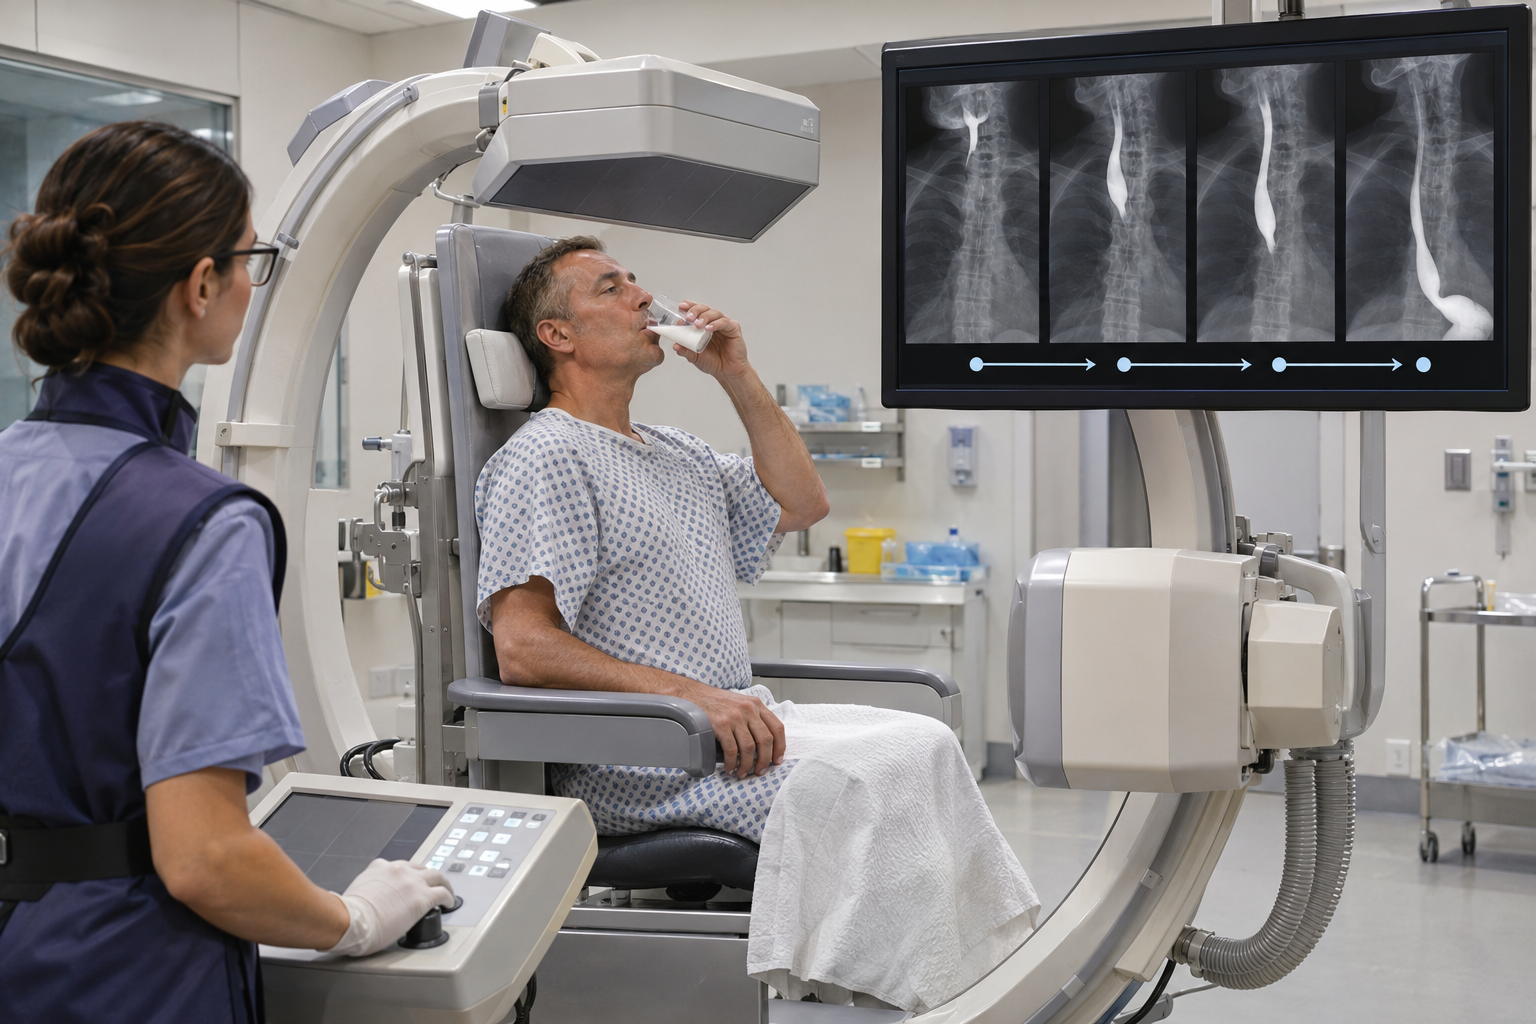
\includegraphics[width=\textwidth,keepaspectratio]{modalities/infographics/fluoroscopy_realistic.png}
\end{center}
\begin{center}\footnotesize Fluoroscopy captures X-ray images over time to show motion, contrast transit, or device movement; the sequence carries radiation exposure. AI-generated illustration; monitor images are not clinical studies.\end{center}

\section{Overview}
Fluoroscopy records a sequence of X-ray images. During a swallow, for example, the images show whether contrast passes below the vocal folds and whether this happens before, during, or after the swallow. A single frame may show the contrast in the airway but miss how it got there.

\section{Where fluoroscopy is used}
The 100 entries below describe diseases, structural abnormalities, and events observed during an examination. Some overlap. The entries include selected and historical uses alongside examinations in current routine practice. In angiography and arthrography, the findings described are visible on the contrast X-ray images themselves. An injection performed under fluoroscopy for a subsequent CT or MRI study serves a different purpose.

\subsection{Esophagus}
\textbf{Examinations.} A barium esophagram assesses contour and transit. A dedicated leak esophagram for suspected perforation often begins with water-soluble contrast. A negative initial study can miss a small leak.

\begin{enumerate}[leftmargin=*,itemsep=0.45em,topsep=0.4em]
\item \textbf{Achalasia.}\par\noindent\textbf{Why order fluoroscopy:} Dysphagia to liquids and solids, regurgitation, or unexplained esophageal retention may prompt a timed barium esophagram.\par\noindent\textbf{What to look for:} Smooth distal tapering, delayed emptying, and retained barium.\par\noindent\textbf{Role and sufficiency:} The study can strongly suggest achalasia and quantify emptying, but manometry confirms the motor disorder and endoscopy excludes a mechanical obstruction.
\item \textbf{Distal esophageal spasm.}\par\noindent\textbf{Why order fluoroscopy:} Intermittent dysphagia or noncardiac chest pain may lead to a dynamic esophagram.\par\noindent\textbf{What to look for:} Premature, nonpropulsive contractions and an intermittent corkscrew contour.\par\noindent\textbf{Role and sufficiency:} A normal study between episodes does not exclude spasm; high-resolution manometry is needed to establish the motility diagnosis.
\item \textbf{Epiphrenic diverticulum.}\par\noindent\textbf{Why order fluoroscopy:} Dysphagia, regurgitation, or retained food may prompt a barium study.\par\noindent\textbf{What to look for:} A contrast-filled pouch arising from the distal esophagus and its emptying.\par\noindent\textbf{Role and sufficiency:} Fluoroscopy usually demonstrates the pouch, but associated motility disorders require manometric assessment.
\item \textbf{Esophageal carcinoma.}\par\noindent\textbf{Why order fluoroscopy:} Progressive dysphagia, painful swallowing, or weight loss may prompt an esophagram when luminal narrowing is suspected.\par\noindent\textbf{What to look for:} Irregular shouldered narrowing, mucosal destruction, or a filling defect.\par\noindent\textbf{Role and sufficiency:} The study localizes and characterizes obstruction but cannot establish cancer; endoscopy with biopsy is required.
\item \textbf{Esophageal dysmotility.}\par\noindent\textbf{Why order fluoroscopy:} Swallowing difficulty, regurgitation, or unexplained transit symptoms may prompt real-time assessment.\par\noindent\textbf{What to look for:} Weak or disordered contractions, delayed clearance, and retained contrast.\par\noindent\textbf{Role and sufficiency:} It shows bolus transit during the sampled examination, but intermittent symptoms may not occur and manometry defines many specific motor disorders.
\item \textbf{Esophageal fistula.}\par\noindent\textbf{Why order fluoroscopy:} Coughing with swallowing, recurrent aspiration, or suspected communication after surgery or infection may prompt a contrast study.\par\noindent\textbf{What to look for:} Contrast passing through an abnormal tract into the airway or another organ.\par\noindent\textbf{Role and sufficiency:} Demonstrating the tract can establish its presence and location; a small or intermittently sealed fistula may be missed, requiring CT or endoscopy.
\item \textbf{Esophageal perforation.}\par\noindent\textbf{Why order fluoroscopy:} Severe chest pain after vomiting, instrumentation, or trauma raises urgent concern for a leak.\par\noindent\textbf{What to look for:} Extraluminal contrast, the leak site, and any contained collection.\par\noindent\textbf{Role and sufficiency:} A positive study demonstrates leakage, but a negative examination does not fully exclude a small perforation; CT and clinical assessment are used when suspicion remains.
\item \textbf{Esophageal stricture.}\par\noindent\textbf{Why order fluoroscopy:} Solid-food dysphagia or food impaction may prompt measurement of a narrowed segment.\par\noindent\textbf{What to look for:} Persistent narrowing, its length, contour, and effect on bolus passage.\par\noindent\textbf{Role and sufficiency:} Fluoroscopy maps the lumen but usually cannot determine the cause; endoscopy and biopsy may be needed, particularly for new or irregular strictures.
\item \textbf{Esophageal web.}\par\noindent\textbf{Why order fluoroscopy:} Intermittent solid-food dysphagia may prompt a targeted cervical esophagram.\par\noindent\textbf{What to look for:} A thin shelf-like filling defect, often anterior and proximal.\par\noindent\textbf{Role and sufficiency:} A well-positioned study can show the web; subtle lesions may be missed without appropriate views and distension.
\item \textbf{Gastroesophageal reflux.}\par\noindent\textbf{Why order fluoroscopy:} Reflux symptoms may lead to evaluation for anatomy or associated complications, not to prove ordinary reflux episodes.\par\noindent\textbf{What to look for:} Reflux observed during the examination, hiatal hernia, or stricture.\par\noindent\textbf{Role and sufficiency:} Reflux may occur in healthy people and may be absent during the brief study; fluoroscopy alone neither confirms nor excludes GERD.
\item \textbf{Hiatal hernia.}\par\noindent\textbf{Why order fluoroscopy:} Dysphagia, reflux symptoms, or suspected intrathoracic stomach may prompt a dynamic upper GI study.\par\noindent\textbf{What to look for:} Stomach above the diaphragm and the position of the gastroesophageal junction.\par\noindent\textbf{Role and sufficiency:} Fluoroscopy can demonstrate and classify many hernias, though size can vary with position and strain; CT or endoscopy may be used for complications.
\item \textbf{Schatzki ring.}\par\noindent\textbf{Why order fluoroscopy:} Intermittent solid-food sticking or food impaction may prompt a distended esophagram.\par\noindent\textbf{What to look for:} A thin circumferential ring at the gastroesophageal junction and narrowing of the lumen.\par\noindent\textbf{Role and sufficiency:} A properly performed study often shows the ring, but endoscopy may be needed when symptoms persist or treatment is planned.
\item \textbf{Zenker diverticulum.}\par\noindent\textbf{Why order fluoroscopy:} Oropharyngeal dysphagia, regurgitation of undigested food, halitosis, or cough after eating may prompt a pharyngoesophagram.\par\noindent\textbf{What to look for:} A posterior pouch above the cricopharyngeus, its size, and retention or aspiration of contrast.\par\noindent\textbf{Role and sufficiency:} Fluoroscopy usually defines the pouch and swallowing mechanics; endoscopy is not a substitute for initial anatomic mapping and should be approached cautiously.
\end{enumerate}

\subsection{Oropharyngeal swallowing disorders}
\textbf{Examinations.} Videofluoroscopic swallowing study (VFSS), modified barium swallow.

\begin{enumerate}[leftmargin=*,itemsep=0.45em,topsep=0.4em]
\item \textbf{Cricopharyngeal dysfunction.}\par\noindent\textbf{Why order VFSS:} A sensation of food sticking in the throat, repeated swallows, or post-swallow residue may prompt dynamic swallowing assessment.\par\noindent\textbf{What to look for:} Reduced opening of the pharyngoesophageal segment, bolus hold-up, and residue.\par\noindent\textbf{Role and sufficiency:} VFSS shows the movement pattern but not every cause of impaired opening; clinical swallowing assessment and sometimes endoscopy/manometry add context.
\item \textbf{Delayed initiation of the pharyngeal swallow.}\par\noindent\textbf{Why order VFSS:} Coughing, choking, or delayed swallowing with meals may prompt evaluation of swallow timing.\par\noindent\textbf{What to look for:} Bolus entering the pharynx before the swallow response begins, interpreted relative to bolus consistency and location.\par\noindent\textbf{Role and sufficiency:} VFSS directly observes sampled swallows, but results vary with task and bolus; it does not by itself identify the neurologic or muscular cause.
\item \textbf{Laryngeal penetration.}\par\noindent\textbf{Why order VFSS:} Coughing or a wet voice during meals may prompt assessment of airway protection.\par\noindent\textbf{What to look for:} Contrast entering the laryngeal vestibule but remaining above the vocal folds; record depth and whether it clears.\par\noindent\textbf{Role and sufficiency:} VFSS identifies penetration during tested swallows, but a limited sample cannot guarantee safety with every food or meal.
\item \textbf{Oropharyngeal dysphagia.}\par\noindent\textbf{Why order VFSS:} Difficulty initiating a swallow, coughing with liquids, nasal regurgitation, or unexplained aspiration may prompt videofluoroscopy.\par\noindent\textbf{What to look for:} Oral transfer, swallow timing, pharyngeal clearance, airway entry, and upper esophageal opening.\par\noindent\textbf{Role and sufficiency:} VFSS characterizes mechanics and helps guide diet or therapy; it does not alone establish the underlying disease or represent every meal.
\item \textbf{Pharyngeal muscle weakness.}\par\noindent\textbf{Why order VFSS:} Weak cough, repeated swallows, or a sensation of residue may prompt functional assessment.\par\noindent\textbf{What to look for:} Reduced pharyngeal constriction and retained contrast after the swallow.\par\noindent\textbf{Role and sufficiency:} Residue supports impaired clearance but is nonspecific; correlate with examination, neurologic history, and other swallowing findings.
\item \textbf{Pulmonary aspiration.}\par\noindent\textbf{Why order VFSS:} Coughing, choking, recurrent chest infections, or suspected silent aspiration may prompt a videofluoroscopic swallow study.\par\noindent\textbf{What to look for:} Contrast passing below the vocal folds, including timing and whether it is expelled.\par\noindent\textbf{Role and sufficiency:} Aspiration observed during the test confirms airway entry for that sampled swallow, but a negative study cannot exclude intermittent aspiration in other conditions or at other times.
\item \textbf{Velopharyngeal insufficiency.}\par\noindent\textbf{Why order VFSS:} Nasal escape of liquids, hypernasal speech, or swallowing difficulty may prompt dynamic assessment.\par\noindent\textbf{What to look for:} Contrast entering the nasopharynx through incomplete velopharyngeal closure.\par\noindent\textbf{Role and sufficiency:} Fluoroscopy demonstrates closure during the tested task; speech-language assessment and targeted ENT evaluation determine functional impact and cause.
\end{enumerate}

\subsection{Stomach and duodenum}
\textbf{Examination.} Upper gastrointestinal contrast series.

\begin{enumerate}[leftmargin=*,itemsep=0.45em,topsep=0.4em]
\item \textbf{Annular pancreas.}\par\noindent\textbf{Why order fluoroscopy:} Recurrent vomiting or duodenal obstruction, especially in an infant, may prompt an upper GI series.\par\noindent\textbf{What to look for:} Fixed narrowing of the second duodenal portion and delayed passage.\par\noindent\textbf{Role and sufficiency:} The narrowing is an indirect sign; CT or MRI can demonstrate pancreatic tissue encircling the duodenum and define anatomy.
\item \textbf{Duodenal diverticulum.}\par\noindent\textbf{Why order fluoroscopy:} Postprandial discomfort, bleeding, or suspected obstruction may prompt luminal assessment.\par\noindent\textbf{What to look for:} A contrast-filled pouch communicating with the duodenal lumen, including its neck and position.\par\noindent\textbf{Role and sufficiency:} Fluoroscopy can establish a patent diverticulum, but cross-sectional imaging or endoscopy may be needed for complications or an uncertain cause of symptoms.
\item \textbf{Duodenal stenosis.}\par\noindent\textbf{Why order fluoroscopy:} Persistent vomiting or suspected proximal small-bowel obstruction may prompt an upper GI series.\par\noindent\textbf{What to look for:} The level, length, and severity of fixed narrowing and upstream hold-up.\par\noindent\textbf{Role and sufficiency:} It maps luminal transit but may not identify the cause; endoscopy or CT/MRI is used when a mass or extrinsic compression is suspected.
\item \textbf{Duodenal ulcer.}\par\noindent\textbf{Why order fluoroscopy:} Epigastric pain or suspected ulcer-related deformity may lead to contrast examination when endoscopy is unavailable or unsuitable.\par\noindent\textbf{What to look for:} A niche projecting beyond the expected contour, with bulb deformity or scarring.\par\noindent\textbf{Role and sufficiency:} Fluoroscopy may show an ulcer but cannot biopsy or reliably exclude malignancy; endoscopy is preferred for diagnosis and sampling.
\item \textbf{Gastric carcinoma.}\par\noindent\textbf{Why order fluoroscopy:} Early satiety, weight loss, anemia, or persistent vomiting may prompt evaluation of gastric contour if an upper GI series is selected.\par\noindent\textbf{What to look for:} Irregular filling defect, shouldered narrowing, rigidity, or poor distensibility.\par\noindent\textbf{Role and sufficiency:} These findings raise suspicion but are not diagnostic; endoscopy with biopsy is required.
\item \textbf{Gastric diverticulum.}\par\noindent\textbf{Why order fluoroscopy:} A suspected anatomic pouch in a patient with upper abdominal symptoms may prompt an upper GI series.\par\noindent\textbf{What to look for:} A contrast-filled outpouching, usually near the gastric fundus, in more than one projection.\par\noindent\textbf{Role and sufficiency:} Fluoroscopy can demonstrate a communicating pouch; CT may clarify its location or distinguish it from an adjacent lesion.
\item \textbf{Gastric outlet obstruction.}\par\noindent\textbf{Why order fluoroscopy:} Recurrent nonbilious vomiting, early satiety, or gastric distension may prompt assessment of passage through the pylorus.\par\noindent\textbf{What to look for:} Persistent hold-up, narrowing, and the level of transition rather than delayed emptying alone.\par\noindent\textbf{Role and sufficiency:} It confirms impaired transit during the study but may not determine the cause; endoscopy and cross-sectional imaging assess structural disease.
\item \textbf{Gastric ulcer.}\par\noindent\textbf{Why order fluoroscopy:} Persistent epigastric pain or suspected ulcer-related deformity may prompt an upper GI contrast study in selected settings.\par\noindent\textbf{What to look for:} Contrast pooling in a crater, surrounding folds, and any mass-like or irregular contour.\par\noindent\textbf{Role and sufficiency:} It cannot provide tissue diagnosis or reliably distinguish benign from malignant ulceration; endoscopy with biopsy is needed when indicated.
\item \textbf{Gastric volvulus.}\par\noindent\textbf{Why order fluoroscopy:} Acute epigastric or chest pain with retching and inability to pass a tube can raise concern for volvulus.\par\noindent\textbf{What to look for:} Abnormal gastric axis, compartmentalization, beaking, and obstruction at the outlet.\par\noindent\textbf{Role and sufficiency:} An upper GI series can demonstrate rotation and impaired passage in a stable patient; urgent CT and clinical assessment define complications such as ischemia or perforation.
\item \textbf{Intestinal malrotation.}\par\noindent\textbf{Why order fluoroscopy:} Bilious vomiting in an infant or intermittent obstructive symptoms may prompt urgent upper GI evaluation.\par\noindent\textbf{What to look for:} Course of the duodenum and position of the duodenojejunal junction, with attention to corkscrew configuration.\par\noindent\textbf{Role and sufficiency:} A technically adequate study is the principal luminal test, but equivocal results require expert review and often ultrasound or cross-sectional imaging; do not delay urgent surgical assessment when volvulus is suspected.
\item \textbf{Linitis plastica.}\par\noindent\textbf{Why order fluoroscopy:} Early satiety, weight loss, or suspected infiltrative gastric disease may prompt assessment of distensibility.\par\noindent\textbf{What to look for:} Diffuse narrowing, rigid poorly distensible stomach, and thickened folds.\par\noindent\textbf{Role and sufficiency:} The pattern suggests infiltration but cannot establish its cause; endoscopic biopsies, sometimes repeated or obtained with EUS, are needed.
\item \textbf{Midgut volvulus.}\par\noindent\textbf{Why order fluoroscopy:} Acute bilious vomiting and suspected malrotation-related obstruction demand urgent evaluation.\par\noindent\textbf{What to look for:} Abnormally positioned duodenojejunal junction and corkscrew twisting of the duodenum or proximal jejunum.\par\noindent\textbf{Role and sufficiency:} Fluoroscopy can identify the characteristic configuration, but urgent management is driven by the clinical picture and surgical assessment; a negative or equivocal study does not safely exclude volvulus if suspicion remains high.
\item \textbf{Superior mesenteric artery syndrome.}\par\noindent\textbf{Why order fluoroscopy:} Postprandial pain, early satiety, and bilious vomiting, particularly after weight loss, may prompt assessment of duodenal transit.\par\noindent\textbf{What to look for:} Compression at the third duodenal portion, proximal dilatation, and improved passage with position change.\par\noindent\textbf{Role and sufficiency:} Fluoroscopy demonstrates functional obstruction but does not prove vascular compression; CT or MRI measures the aortomesenteric relationship and excludes other causes.
\end{enumerate}

\subsection{Small intestine}
\textbf{Examinations.} Small bowel follow-through and enteroclysis examine the lumen. In selected patients with known obstruction, a water-soluble contrast challenge assesses progression to the colon. CT generally evaluates the site, cause, and complications of acute obstruction.

\begin{enumerate}[leftmargin=*,itemsep=0.45em,topsep=0.4em]
\item \textbf{Crohn disease.}\par\noindent\textbf{Why order fluoroscopy:} Chronic diarrhea, abdominal pain, or suspected stricture may prompt small-bowel contrast evaluation when enterography is unavailable or for selected transit questions.\par\noindent\textbf{What to look for:} Skip areas, aphthous or longitudinal ulcers, cobblestoning, and fixed narrowing such as a string sign.\par\noindent\textbf{Role and sufficiency:} It depicts mucosal contour and strictures but not transmural complications well; CT or MR enterography and endoscopy are generally more comprehensive.
\item \textbf{Small bowel diverticulosis.}\par\noindent\textbf{Why order fluoroscopy:} Unexplained anemia, pain, or suspected diverticular anatomy may prompt a small-bowel series.\par\noindent\textbf{What to look for:} One or more contrast-filled outpouchings arising from the bowel, distinguished from overlapping loops by tracking them across views.\par\noindent\textbf{Role and sufficiency:} Fluoroscopy can show communicating diverticula but may miss complications or lesions outside the lumen; CT is used for suspected inflammation or bleeding complications.
\item \textbf{Small bowel dysmotility.}\par\noindent\textbf{Why order fluoroscopy:} Persistent bloating, vomiting, or transit symptoms after mechanical obstruction is considered may prompt a timed small-bowel study.\par\noindent\textbf{What to look for:} Delayed progression, ineffective propulsion, or disorganized transit across serial images.\par\noindent\textbf{Role and sufficiency:} Transit is affected by preparation, medications, and technique; fluoroscopy suggests abnormal motility but does not specify its cause or replace targeted physiological testing.
\item \textbf{Small bowel fistula.}\par\noindent\textbf{Why order fluoroscopy:} Drainage, recurrent infection, or suspected communication after surgery or inflammatory disease may prompt contrast evaluation.\par\noindent\textbf{What to look for:} Contrast traversing an abnormal tract between loops or into an adjacent organ.\par\noindent\textbf{Role and sufficiency:} A visible tract confirms communication during the study, but intermittent or narrow fistulas may not opacify; CT/MR enterography or endoscopy can provide additional mapping.
\item \textbf{Small bowel obstruction.}\par\noindent\textbf{Why order fluoroscopy:} Vomiting, distension, and failure to pass stool or gas may prompt a water-soluble contrast challenge in selected patients with suspected adhesive obstruction.\par\noindent\textbf{What to look for:} Delayed passage at a transition and whether contrast reaches the colon within the protocol interval.\par\noindent\textbf{Role and sufficiency:} The challenge helps assess progression but does not reliably identify the cause or complications; CT is generally used to locate the transition and evaluate ischemia or closed loop.
\item \textbf{Small bowel strictures.}\par\noindent\textbf{Why order fluoroscopy:} Intermittent obstructive symptoms or known inflammatory disease may prompt mapping of a narrowed segment.\par\noindent\textbf{What to look for:} Persistent focal or multifocal narrowing, length, upstream dilatation, and transit delay.\par\noindent\textbf{Role and sufficiency:} It demonstrates luminal caliber but cannot reliably distinguish inflammatory from fibrotic narrowing or show extraluminal disease; enterography and endoscopy may be needed.
\item \textbf{Small bowel tumors.}\par\noindent\textbf{Why order fluoroscopy:} Occult bleeding, anemia, or unexplained obstructive symptoms may prompt evaluation of the small-bowel lumen.\par\noindent\textbf{What to look for:} Persistent filling defect, irregular narrowing, mucosal destruction, or shouldering.\par\noindent\textbf{Role and sufficiency:} A mass can be localized, but fluoroscopy cannot determine histology or fully stage it; capsule/deep enteroscopy and CT or MR enterography are selected according to the clinical question.
\end{enumerate}

\subsection{Colon and rectum}
\textbf{Examination.} Contrast enema. Water-soluble contrast is used when evaluating a suspected postoperative leak. In children with suspected ileocolic intussusception, ultrasound is usually the first examination. A fluoroscopic air or liquid enema can show the intussusception and document its reduction.

\begin{enumerate}[leftmargin=*,itemsep=0.45em,topsep=0.4em]
\item \textbf{Colonic anastomotic leakage.}\par\noindent\textbf{Why order fluoroscopy:} Fever, pain, or concerning drain output after colorectal surgery may prompt a water-soluble contrast enema to assess an anastomosis.\par\noindent\textbf{What to look for:} Contrast outside the bowel at the surgical join and the extent of any contained leak.\par\noindent\textbf{Role and sufficiency:} A demonstrated leak is useful, but small or intermittently sealed defects may be missed; CT with appropriate contrast and clinical assessment are needed when suspicion persists.
\item \textbf{Colonic diverticulosis.}\par\noindent\textbf{Why order fluoroscopy:} A contrast enema may demonstrate diverticula when luminal anatomy is being assessed for another reason.\par\noindent\textbf{What to look for:} Multiple small contrast-filled outpouchings beyond the expected colonic contour.\par\noindent\textbf{Role and sufficiency:} It can establish diverticular anatomy but does not diagnose acute diverticulitis or explain bleeding; CT or endoscopy is selected for those questions.
\item \textbf{Colonic fistula.}\par\noindent\textbf{Why order fluoroscopy:} Fecaluria, pneumaturia, vaginal stool passage, or persistent drainage may prompt a targeted contrast study.\par\noindent\textbf{What to look for:} Contrast crossing from colon into an adjacent organ or tract.\par\noindent\textbf{Role and sufficiency:} Direct opacification confirms communication, but a narrow or intermittently patent fistula may be missed; CT and endoscopy help identify the cause and surrounding disease.
\item \textbf{Colonic strictures.}\par\noindent\textbf{Why order fluoroscopy:} Altered bowel habits, obstructive symptoms, or postoperative narrowing may prompt luminal mapping.\par\noindent\textbf{What to look for:} Fixed narrowing, length, contour, and proximal dilatation.\par\noindent\textbf{Role and sufficiency:} The enema defines caliber but not etiology; colonoscopy with biopsy or CT is required when malignancy or extrinsic disease is possible.
\item \textbf{Colorectal carcinoma.}\par\noindent\textbf{Why order fluoroscopy:} Obstructive symptoms may lead to contrast evaluation when colonoscopy cannot traverse a narrowing or is not feasible.\par\noindent\textbf{What to look for:} Short irregular shouldered narrowing, annular constriction, or persistent filling defect.\par\noindent\textbf{Role and sufficiency:} These signs suggest a tumor but cannot establish histology; colonoscopy and biopsy are needed, and CT stages disease.
\item \textbf{Hirschsprung disease.}\par\noindent\textbf{Why order fluoroscopy:} Delayed passage of meconium, abdominal distension, and bilious vomiting in an infant may prompt a contrast enema after stabilization.\par\noindent\textbf{What to look for:} A narrow distal aganglionic segment with a transition to dilated proximal colon and a reversed rectosigmoid ratio.\par\noindent\textbf{Role and sufficiency:} The enema supports localization, but a normal study does not exclude disease; rectal suction biopsy establishes the diagnosis.
\item \textbf{Meconium ileus.}\par\noindent\textbf{Why order fluoroscopy:} A newborn with distal bowel obstruction and failure to pass meconium may undergo a water-soluble contrast enema, which can also be therapeutic.\par\noindent\textbf{What to look for:} Microcolon and terminal ileal filling defects from inspissated meconium.\par\noindent\textbf{Role and sufficiency:} The pattern supports meconium ileus but microcolon is not specific; clinical assessment and evaluation for cystic fibrosis are important.
\item \textbf{Neonatal small left colon syndrome.}\par\noindent\textbf{Why order fluoroscopy:} A newborn with abdominal distension and delayed stool passage may undergo contrast enema to assess distal obstruction.\par\noindent\textbf{What to look for:} A narrow descending colon and sigmoid with an abrupt caliber change near the splenic flexure.\par\noindent\textbf{Role and sufficiency:} The appearance supports the diagnosis and the enema may relieve obstruction, but clinical course and exclusion of Hirschsprung disease are needed if symptoms persist.
\item \textbf{Pediatric ileocolic intussusception.}\par\noindent\textbf{Why order fluoroscopy:} Episodic severe abdominal pain, vomiting, lethargy, or bloody stool after ultrasound suggests intussusception may prompt image-guided enema reduction.\par\noindent\textbf{What to look for:} A meniscus or coiled-spring filling defect and, during treatment, reflux of contrast into the terminal ileum indicating reduction.\par\noindent\textbf{Role and sufficiency:} Enema is diagnostic and therapeutic in suitable stable patients; perforation or peritonitis changes management, and ultrasound is generally the initial diagnostic examination.
\item \textbf{Sigmoid volvulus.}\par\noindent\textbf{Why order fluoroscopy:} Marked distension, constipation, and obstructive symptoms may prompt contrast enema in a stable patient when decompression is being considered.\par\noindent\textbf{What to look for:} Smooth tapering to a bird-beak at the twist and failure of contrast to pass.\par\noindent\textbf{Role and sufficiency:} It can show the level and sometimes aid decompression, but CT is commonly used to assess ischemia or perforation; peritonitis or suspected bowel compromise requires urgent surgical evaluation.
\item \textbf{Ulcerative colitis.}\par\noindent\textbf{Why order fluoroscopy:} Contrast enema now has limited use and may be considered only for selected structural questions outside acute severe colitis.\par\noindent\textbf{What to look for:} Chronic loss of haustra, shortening, and a featureless lead-pipe contour.\par\noindent\textbf{Role and sufficiency:} These are chronic changes, not a reliable measure of active inflammation; endoscopy with biopsy and clinical assessment guide diagnosis, while barium enema is generally avoided in severe acute disease.
\end{enumerate}

\subsection{Pelvic floor and defecation disorders}
\textbf{Examination.} Fluoroscopic defecography.

\begin{enumerate}[leftmargin=*,itemsep=0.45em,topsep=0.4em]
\item \textbf{Descending perineum syndrome.}\par\noindent\textbf{Why order fluoroscopy:} Excessive straining, incomplete evacuation, or pelvic pressure may prompt defecography.\par\noindent\textbf{What to look for:} Abnormally large perineal descent during strain and evacuation, measured relative to a fixed pelvic line.\par\noindent\textbf{Role and sufficiency:} Defecography documents movement during the test but descent can occur in asymptomatic people; symptoms and anorectal examination determine relevance.
\item \textbf{Dyssynergic defecation.}\par\noindent\textbf{Why order fluoroscopy:} Chronic straining, prolonged toileting, and incomplete evacuation may prompt assessment of coordinated evacuation.\par\noindent\textbf{What to look for:} Failure of the anorectal angle to open, paradoxical narrowing, and retained rectal contrast.\par\noindent\textbf{Role and sufficiency:} Defecography can demonstrate an abnormal pattern, but diagnosis requires compatible symptoms and is usually corroborated with anorectal manometry and balloon expulsion testing.
\item \textbf{Enterocele.}\par\noindent\textbf{Why order fluoroscopy:} Pelvic pressure or obstructed defecation, especially after pelvic surgery, may prompt evacuation imaging.\par\noindent\textbf{What to look for:} Small bowel descending between rectum and vagina during strain; oral contrast can distinguish bowel loops.\par\noindent\textbf{Role and sufficiency:} Defecography shows dynamic descent and its relation to evacuation, but clinical significance depends on symptoms and may require pelvic MRI for broader compartment assessment.
\item \textbf{Rectal intussusception.}\par\noindent\textbf{Why order fluoroscopy:} Obstructed defecation, tenesmus, or incomplete emptying may prompt dynamic evaluation.\par\noindent\textbf{What to look for:} Rectal wall telescoping inward during evacuation and whether it obstructs the outlet.\par\noindent\textbf{Role and sufficiency:} Defecography depicts the event under test conditions, but minor intussusception may be incidental; correlate with symptoms and examination.
\item \textbf{Rectal prolapse.}\par\noindent\textbf{Why order fluoroscopy:} A history of tissue protrusion or obstructed evacuation may prompt defecography when examination does not capture the event.\par\noindent\textbf{What to look for:} Full-thickness rectal wall descending through the anal canal during evacuation.\par\noindent\textbf{Role and sufficiency:} Fluoroscopy can document dynamic prolapse, but visible external prolapse is often diagnosed clinically; the study helps define associated pelvic floor abnormalities.
\item \textbf{Rectocele.}\par\noindent\textbf{Why order fluoroscopy:} Vaginal splinting, incomplete evacuation, or a bulge sensation may prompt defecography.\par\noindent\textbf{What to look for:} Anterior rectal wall pouching into the vagina, its depth, retained contrast, and emptying.\par\noindent\textbf{Role and sufficiency:} A small rectocele is common and may be incidental; imaging alone does not establish the cause of symptoms or need for treatment.
\item \textbf{Sigmoidocele.}\par\noindent\textbf{Why order fluoroscopy:} Pelvic pressure or difficult evacuation may prompt evaluation for a descending sigmoid loop.\par\noindent\textbf{What to look for:} Sigmoid colon entering the cul-de-sac during evacuation and compressing the rectum.\par\noindent\textbf{Role and sufficiency:} Defecography captures dynamic descent, while pelvic MRI can assess multiple compartments; findings require symptom correlation.
\end{enumerate}

\subsection{Urinary system}
\textbf{Examinations.} Voiding cystourethrography (VCUG), retrograde urethrography, retrograde cystography, and video-urodynamics.

\begin{enumerate}[leftmargin=*,itemsep=0.45em,topsep=0.4em]
\item \textbf{Bladder diverticulum.}\par\noindent\textbf{Why order fluoroscopy:} Recurrent infection, incomplete emptying, or suspected outlet obstruction may prompt cystography or VCUG.\par\noindent\textbf{What to look for:} A contrast-filled pouch communicating with the bladder, its size, and residual contrast after voiding.\par\noindent\textbf{Role and sufficiency:} It demonstrates a patent diverticulum but does not determine why it formed; ultrasound, cystoscopy, or urodynamics may clarify associated dysfunction.
\item \textbf{Bladder outlet obstruction.}\par\noindent\textbf{Why order fluoroscopy:} Weak stream, straining, or retention may prompt video-urodynamic evaluation when the level or mechanism is uncertain.\par\noindent\textbf{What to look for:} Failure of the bladder neck or urethra to open normally and the level of narrowing during voiding.\par\noindent\textbf{Role and sufficiency:} Images localize anatomy, but pressure-flow measurements distinguish obstruction from weak detrusor contraction; fluoroscopy alone is insufficient.
\item \textbf{Bladder rupture.}\par\noindent\textbf{Why order fluoroscopy:} Pelvic trauma with hematuria or suspected postoperative injury may prompt retrograde cystography.\par\noindent\textbf{What to look for:} Contrast outside the bladder, within the peritoneal cavity or around the extraperitoneal pelvis, after adequate retrograde filling.\par\noindent\textbf{Role and sufficiency:} Properly performed cystography can demonstrate and classify rupture; passive excreted contrast may miss it, and CT cystography is commonly used in trauma.
\item \textbf{Detrusor-sphincter dyssynergia.}\par\noindent\textbf{Why order fluoroscopy:} Voiding difficulty in a patient with neurologic disease may prompt synchronized video-urodynamics.\par\noindent\textbf{What to look for:} Persistent or paradoxical outlet closure while the detrusor contracts, with interrupted flow or elevated pressure.\par\noindent\textbf{Role and sufficiency:} Fluoroscopy shows outlet behavior but diagnosis depends on synchronized pressure-flow testing and sometimes sphincter electromyography.
\item \textbf{Neurogenic bladder.}\par\noindent\textbf{Why order fluoroscopy:} Neurologic disease with incontinence, retention, recurrent infection, or upper-tract risk may prompt video-urodynamics.\par\noindent\textbf{What to look for:} Bladder contour, compliance-related changes, reflux, outlet coordination, and emptying during measured pressure and flow.\par\noindent\textbf{Role and sufficiency:} The radiographic contour is nonspecific; diagnosis and risk stratification require urodynamic measurements and clinical context.
\item \textbf{Posterior urethral valves.}\par\noindent\textbf{Why order fluoroscopy:} A male infant with poor urinary stream, antenatal hydronephrosis, or urinary infection may undergo VCUG.\par\noindent\textbf{What to look for:} Dilated posterior urethra with abrupt narrowing, bladder trabeculation, and possible reflux.\par\noindent\textbf{Role and sufficiency:} VCUG strongly suggests the obstruction, but cystoscopy confirms and treats the valves; a technically inadequate voiding phase can miss them.
\item \textbf{Urethral diverticulum.}\par\noindent\textbf{Why order fluoroscopy:} Recurrent infection, postvoid dribbling, or a periurethral mass may prompt voiding imaging.\par\noindent\textbf{What to look for:} A contrast-opacified side pouch communicating with the urethra.\par\noindent\textbf{Role and sufficiency:} A patent opening is required for visualization, so a negative study cannot exclude a closed or poorly filling diverticulum; MRI or endoscopy may be needed.
\item \textbf{Urethral rupture.}\par\noindent\textbf{Why order fluoroscopy:} Blood at the meatus, pelvic trauma, or suspected urethral injury may prompt retrograde urethrography before catheterization.\par\noindent\textbf{What to look for:} Contrast extravasation and whether it reaches the proximal urethra or bladder.\par\noindent\textbf{Role and sufficiency:} The study classifies the injury pattern, but does not replace trauma evaluation; avoid blind urethral catheterization when injury is suspected.
\item \textbf{Urethral stricture.}\par\noindent\textbf{Why order fluoroscopy:} Weak stream, retention, or recurrent infection may prompt retrograde urethrography for procedural planning.\par\noindent\textbf{What to look for:} Site, length, caliber, and number of narrowed segments, with proximal urethral filling where possible.\par\noindent\textbf{Role and sufficiency:} It maps luminal anatomy well but may not fully characterize spongiofibrosis; cystoscopy and clinical findings can complement it.
\item \textbf{Urinary fistula.}\par\noindent\textbf{Why order fluoroscopy:} Urine leaking through the vagina, skin, or bowel, or persistent postoperative drainage, may prompt targeted cystography or urethrography.\par\noindent\textbf{What to look for:} Contrast crossing an abnormal communication and the organs involved.\par\noindent\textbf{Role and sufficiency:} Opacification confirms a patent tract, but small or intermittent fistulas can be missed; CT, MRI, endoscopy, or examination may be required to map it.
\item \textbf{Vesicoureteral reflux.}\par\noindent\textbf{Why order fluoroscopy:} Recurrent febrile urinary infections or suspected reflux-related renal injury may prompt VCUG.\par\noindent\textbf{What to look for:} Retrograde contrast entering the ureter and renal collecting system during filling or voiding; grade the extent and persistence.\par\noindent\textbf{Role and sufficiency:} VCUG directly demonstrates reflux during the examination, but intermittent reflux can be missed and the study does not itself measure renal scarring or function.
\end{enumerate}

\subsection{Female reproductive system}
\textbf{Examination.} Hysterosalpingography (HSG) outlines the uterine cavity and communicating tubes. A divided cavity can occur with either a septate or a bicornuate uterus. Three-dimensional transvaginal ultrasound also shows the external fundal contour needed to distinguish them.

\begin{enumerate}[leftmargin=*,itemsep=0.45em,topsep=0.4em]
\item \textbf{Bicornuate uterus.}\par\noindent\textbf{Why order fluoroscopy:} Infertility, recurrent pregnancy loss, or suspected uterine anomaly may prompt hysterosalpingography (HSG) to assess the cavity and tubes.\par\noindent\textbf{What to look for:} Two divergent endometrial cavities.\par\noindent\textbf{Role and sufficiency:} HSG cannot show the external fundal cleft and cannot distinguish a bicornuate from septate uterus alone; 3-D ultrasound or MRI is needed.
\item \textbf{Cavity-distorting uterine fibroids.}\par\noindent\textbf{Why order fluoroscopy:} Infertility or pregnancy loss may prompt HSG to assess whether the cavity is distorted and whether tubes are patent.\par\noindent\textbf{What to look for:} A smooth indentation or filling defect displacing the contrast-filled cavity.\par\noindent\textbf{Role and sufficiency:} HSG suggests distortion but cannot reliably identify a fibroid versus polyp or define its full extent; transvaginal ultrasound, sonohysterography, or hysteroscopy clarifies it.
\item \textbf{Endometrial polyps.}\par\noindent\textbf{Why order fluoroscopy:} HSG performed during infertility evaluation may incidentally reveal an intracavitary filling defect.\par\noindent\textbf{What to look for:} A smooth, persistent defect surrounded by contrast.\par\noindent\textbf{Role and sufficiency:} HSG is not a definitive polyp test; sonohysterography or hysteroscopy directly evaluates the cavity and permits removal or sampling.
\item \textbf{Fallopian tube obstruction.}\par\noindent\textbf{Why order fluoroscopy:} Difficulty conceiving may prompt HSG to assess tubal patency.\par\noindent\textbf{What to look for:} Where contrast stops, whether either tube fills, and whether free peritoneal spill occurs.\par\noindent\textbf{Role and sufficiency:} HSG assesses patency at the time of the test, but proximal spasm or catheter position can mimic blockage; repeat or selective cannulation may be considered.
\item \textbf{Hydrosalpinx.}\par\noindent\textbf{Why order fluoroscopy:} Infertility or suspected distal tubal disease may prompt HSG.\par\noindent\textbf{What to look for:} A dilated, tortuous contrast-filled tube with absent or loculated distal spill.\par\noindent\textbf{Role and sufficiency:} HSG demonstrates tubal morphology and patency but does not assess surrounding adhesions comprehensively; ultrasound or laparoscopy may be needed.
\item \textbf{Intrauterine adhesions (Asherman syndrome).}\par\noindent\textbf{Why order fluoroscopy:} Reduced menstrual flow, infertility, or pregnancy loss may prompt HSG during cavity evaluation.\par\noindent\textbf{What to look for:} Persistent irregular filling defects, cavity distortion, or partial obliteration.\par\noindent\textbf{Role and sufficiency:} HSG can suggest adhesions but cannot directly characterize them; hysteroscopy is the definitive direct assessment and can guide treatment.
\item \textbf{Peritubal adhesions.}\par\noindent\textbf{Why order fluoroscopy:} Infertility or prior pelvic infection/surgery may prompt HSG to evaluate tubal spill.\par\noindent\textbf{What to look for:} Loculated, restricted, or asymmetric contrast spill around a patent tube.\par\noindent\textbf{Role and sufficiency:} These patterns are indirect and do not prove adhesions; laparoscopy can directly assess peritoneal disease when clinically indicated.
\item \textbf{Salpingitis isthmica nodosa.}\par\noindent\textbf{Why order fluoroscopy:} Infertility or recurrent ectopic pregnancy may prompt HSG.\par\noindent\textbf{What to look for:} Multiple small diverticular outpouchings from the proximal isthmic tube.\par\noindent\textbf{Role and sufficiency:} The characteristic pattern can support the diagnosis, but HSG does not assess all tubal or peritoneal causes of infertility.
\item \textbf{Septate uterus.}\par\noindent\textbf{Why order fluoroscopy:} Recurrent pregnancy loss or infertility may lead to HSG during assessment of the cavity.\par\noindent\textbf{What to look for:} Two endometrial channels or a midline filling defect.\par\noindent\textbf{Role and sufficiency:} HSG cannot show the external fundal contour, so it cannot reliably distinguish septate from bicornuate uterus; 3-D transvaginal ultrasound or MRI is required.
\item \textbf{Unicornuate uterus.}\par\noindent\textbf{Why order fluoroscopy:} Infertility, pregnancy loss, or suspected congenital anomaly may prompt HSG.\par\noindent\textbf{What to look for:} A small, asymmetric, curved uterine cavity with a single tubal origin.\par\noindent\textbf{Role and sufficiency:} HSG shows only the communicating cavity; a noncommunicating rudimentary horn may be invisible, so ultrasound or MRI is needed for complete anatomy.
\end{enumerate}

\subsection{Respiratory system}
\textbf{Examinations.} The diaphragm sniff test records hemidiaphragm motion. A separate dynamic airway examination assesses expiratory narrowing in selected cases. In one pediatric study, fluoroscopy detected tracheomalacia in only 5 of 21 children with bronchoscopically confirmed disease. Bronchoscopy permits direct assessment of tracheal and bronchial collapse.

\begin{enumerate}[leftmargin=*,itemsep=0.45em,topsep=0.4em]
\item \textbf{Bronchomalacia.}\par\noindent\textbf{Why order fluoroscopy:} Recurrent wheeze, barking cough, or expiratory distress may prompt dynamic airway imaging when central airway collapse is suspected.\par\noindent\textbf{What to look for:} Excessive expiratory narrowing of a main bronchus, assessed across the breathing cycle.\par\noindent\textbf{Role and sufficiency:} Fluoroscopy sees only portions of the airway and can miss disease; bronchoscopy or dynamic CT is often needed to establish extent.
\item \textbf{Diaphragmatic eventration.}\par\noindent\textbf{Why order fluoroscopy:} An elevated hemidiaphragm with unexplained breathlessness may prompt a sniff test to assess motion.\par\noindent\textbf{What to look for:} Smooth focal or diffuse elevation with preserved but altered excursion, distinguishing it from paradoxical motion where possible.\par\noindent\textbf{Role and sufficiency:} Fluoroscopy shows movement but may not distinguish eventration from weakness; ultrasound and cross-sectional imaging provide complementary structural assessment.
\item \textbf{Diaphragmatic paralysis.}\par\noindent\textbf{Why order fluoroscopy:} Unexplained dyspnea, orthopnea, or an elevated hemidiaphragm may prompt a dynamic sniff test.\par\noindent\textbf{What to look for:} Paradoxical upward motion of the affected side during a brisk sniff, compared with the opposite hemidiaphragm.\par\noindent\textbf{Role and sufficiency:} It supports unilateral paralysis, but effort and bilateral disease can confound results; diaphragm ultrasound and clinical evaluation may be needed.
\item \textbf{Diaphragmatic weakness.}\par\noindent\textbf{Why order fluoroscopy:} Weak cough, orthopnea, or suspected neuromuscular respiratory impairment may prompt motion assessment.\par\noindent\textbf{What to look for:} Reduced excursion or delayed movement during quiet and deep breathing.\par\noindent\textbf{Role and sufficiency:} Low excursion is nonspecific and may reflect poor effort or lung disease; ultrasound thickening and respiratory muscle testing better quantify function.
\item \textbf{Tracheomalacia.}\par\noindent\textbf{Why order fluoroscopy:} Recurrent stridor, cough, or expiratory airway symptoms may lead to dynamic airway fluoroscopy in selected cases.\par\noindent\textbf{What to look for:} Marked expiratory reduction in tracheal caliber and the location/length of collapse.\par\noindent\textbf{Role and sufficiency:} Fluoroscopy may miss collapse and is not definitive; dynamic bronchoscopy directly assesses the airway, with dynamic CT as another option.
\end{enumerate}

\subsection{Cardiovascular system}
\textbf{Examination.} Catheter arteriography and contrast venography outline the patent lumen. For suspected lower-extremity deep vein thrombosis, duplex ultrasound is the usual initial examination. For suspected pulmonary embolism requiring imaging, CT pulmonary angiography or a ventilation-perfusion study is generally used.

\begin{enumerate}[leftmargin=*,itemsep=0.45em,topsep=0.4em]
\item \textbf{Arterial aneurysm.}\par\noindent\textbf{Why order fluoroscopy:} Catheter angiography is generally used when noninvasive imaging is insufficient or an endovascular procedure is planned.\par\noindent\textbf{What to look for:} Dilatation of the contrast-filled lumen, branch origins, and distal runoff; mural thrombus can make the lumen underestimate outer aneurysm size.\par\noindent\textbf{Role and sufficiency:} Angiography maps the patent channel but CTA or ultrasound is usually better for total diameter and surveillance.
\item \textbf{Arterial dissection.}\par\noindent\textbf{Why order fluoroscopy:} Catheter angiography may be selected to define branch-vessel compromise or guide intervention after CTA/MRA.\par\noindent\textbf{What to look for:} Intimal flap, double lumen, tapered narrowing, or branch malperfusion.\par\noindent\textbf{Role and sufficiency:} It depicts the opacified lumen but may miss a thrombosed false lumen or intramural hematoma; cross-sectional angiography is usually the initial diagnostic study.
\item \textbf{Arteriovenous fistula.}\par\noindent\textbf{Why order fluoroscopy:} Bruit, abnormal venous pressure, or suspected shunting may prompt catheter angiography when localization or treatment planning is needed.\par\noindent\textbf{What to look for:} Early venous filling through a direct communication and the feeding vessel.\par\noindent\textbf{Role and sufficiency:} Angiography demonstrates flow anatomy and can guide closure, but Doppler ultrasound, CTA, or MRA may establish the diagnosis noninvasively.
\item \textbf{Arteriovenous malformation.}\par\noindent\textbf{Why order fluoroscopy:} Hemorrhage, neurologic symptoms, or a known vascular lesion may lead to catheter angiography for detailed angioarchitecture or embolization planning.\par\noindent\textbf{What to look for:} Feeding arteries, nidus, early draining veins, and venous outflow.\par\noindent\textbf{Role and sufficiency:} Digital subtraction angiography is highly detailed for flow anatomy, but CT/MRI assess surrounding tissue and hemorrhage; findings must be interpreted with those studies.
\item \textbf{Carotid artery stenosis.}\par\noindent\textbf{Why order fluoroscopy:} Catheter angiography is reserved for selected discordant noninvasive studies or when intervention is planned.\par\noindent\textbf{What to look for:} Site and degree of luminal narrowing, plaque contour, and distal flow.\par\noindent\textbf{Role and sufficiency:} It quantifies lumen but is invasive and carries embolic risk; duplex ultrasound, CTA, or MRA usually provide initial assessment.
\item \textbf{Cerebral vasospasm.}\par\noindent\textbf{Why order fluoroscopy:} New neurologic deficit after subarachnoid hemorrhage may prompt angiography when endovascular treatment is considered.\par\noindent\textbf{What to look for:} Segmental narrowing compared with prior or unaffected vessels and delayed distal filling.\par\noindent\textbf{Role and sufficiency:} Angiography depicts narrowing and permits treatment, but transcranial Doppler and CTA are commonly used for screening; narrowing alone does not establish symptomatic ischemia.
\item \textbf{Coronary artery disease.}\par\noindent\textbf{Why order fluoroscopy:} High-risk symptoms or noninvasive evidence of ischemia may lead to invasive coronary angiography when revascularization is being considered.\par\noindent\textbf{What to look for:} Stenosis location, severity, lesion length, branch involvement, and flow.\par\noindent\textbf{Role and sufficiency:} Angiography defines lumen but visual severity does not always indicate physiological significance; FFR/iFR or intravascular imaging may be needed, and it is not a screening test.
\item \textbf{Deep vein thrombosis.}\par\noindent\textbf{Why order fluoroscopy:} Contrast venography is now uncommon and may be reserved for selected complex cases or intervention planning.\par\noindent\textbf{What to look for:} Intraluminal filling defect, abrupt cutoff, and collateral pathways.\par\noindent\textbf{Role and sufficiency:} It can outline venous obstruction but is invasive; compression duplex ultrasound is the usual initial test.
\item \textbf{Intracranial aneurysm.}\par\noindent\textbf{Why order fluoroscopy:} Catheter angiography may follow CTA/MRA when small aneurysm anatomy is uncertain or treatment is planned.\par\noindent\textbf{What to look for:} Sac size and shape, neck, branch incorporation, and flow pattern in multiple projections.\par\noindent\textbf{Role and sufficiency:} It provides detailed lumen anatomy but is invasive and may not show thrombus or adjacent tissue; CTA/MRA are commonly used for initial detection and follow-up.
\item \textbf{Peripheral arterial disease.}\par\noindent\textbf{Why order fluoroscopy:} Lifestyle-limiting symptoms or threatened limb with a plan for revascularization may prompt catheter arteriography.\par\noindent\textbf{What to look for:} Stenoses, occlusions, lesion length, collateral supply, and distal runoff.\par\noindent\textbf{Role and sufficiency:} It maps treatable lumen and permits intervention, but ABI and duplex/CTA/MRA usually establish disease noninvasively and assess the whole vessel wall.
\item \textbf{Pulmonary embolism.}\par\noindent\textbf{Why order fluoroscopy:} Catheter pulmonary angiography is now mainly used during selected catheter-directed treatment or when other tests are inconclusive.\par\noindent\textbf{What to look for:} Intraluminal filling defects, abrupt vessel cutoff, and regional perfusion changes.\par\noindent\textbf{Role and sufficiency:} It can demonstrate emboli but is invasive; CT pulmonary angiography or V/Q imaging is generally used for diagnosis.
\item \textbf{Renal artery stenosis.}\par\noindent\textbf{Why order fluoroscopy:} Catheter angiography may be considered when noninvasive imaging is inconclusive and intervention is planned.\par\noindent\textbf{What to look for:} Focal narrowing, lesion location, pressure gradient when measured, and downstream perfusion.\par\noindent\textbf{Role and sufficiency:} It shows lumen but stenosis alone does not prove renovascular hypertension or benefit from treatment; duplex, CTA/MRA, and clinical assessment guide selection.
\item \textbf{Venous stenosis.}\par\noindent\textbf{Why order fluoroscopy:} Swelling, access dysfunction, or collateral veins may prompt catheter venography when treatment is contemplated.\par\noindent\textbf{What to look for:} Narrowed segment, delayed outflow, collateralization, and pressure effects where measured.\par\noindent\textbf{Role and sufficiency:} Venography defines lumen and supports intervention, while ultrasound or CT/MR venography may be preferred for initial evaluation depending on site.
\end{enumerate}

\subsection{Musculoskeletal system}
\textbf{Examinations.} Wrist cineradiography and conventional shoulder arthrography. In acute adult cervical trauma requiring imaging, CT is generally the initial examination. Dynamic fluoroscopy has no routine role in clearing the injured neck.

\begin{enumerate}[leftmargin=*,itemsep=0.45em,topsep=0.4em]
\item \textbf{Carpal instability.}\par\noindent\textbf{Why order fluoroscopy:} Pain, clicking, or weakness with wrist loading despite nondiagnostic static radiographs may prompt dynamic cineradiography.\par\noindent\textbf{What to look for:} Abnormal carpal alignment or asynchronous movement through radial/ulnar deviation and flexion/extension.\par\noindent\textbf{Role and sufficiency:} Dynamic views may reveal instability not seen at rest, but dedicated radiographs and MRI/CT assess associated ligament or bone injury.
\item \textbf{Full-thickness rotator cuff tear.}\par\noindent\textbf{Why order fluoroscopy:} Conventional shoulder arthrography may be used when MRI is unsuitable and a communicating full-thickness tear is suspected.\par\noindent\textbf{What to look for:} Intra-articular contrast passing through the cuff into the subacromial-subdeltoid bursa.\par\noindent\textbf{Role and sufficiency:} A communicating tear is demonstrated, but ultrasound or MRI more directly evaluates tendon anatomy and partial tears; arthrography is now less commonly used.
\item \textbf{Scapholunate instability.}\par\noindent\textbf{Why order fluoroscopy:} Wrist pain or clicking after injury with normal static views may prompt stress radiographs or cineradiography.\par\noindent\textbf{What to look for:} Dynamic widening of the scapholunate interval and abnormal carpal rotation during motion.\par\noindent\textbf{Role and sufficiency:} It can reveal dynamic instability, but does not fully characterize ligament integrity; MRI, MR arthrography, or arthroscopy may be needed.
\end{enumerate}

\subsection{Summary}
\begin{center}
\begin{tabular}{@{}lr@{}}
\toprule
\textbf{Anatomical system} & \textbf{Entries} \\
\midrule
Cardiovascular system & 13 \\
Colon and rectum & 11 \\
Esophagus & 13 \\
Female reproductive system & 10 \\
Musculoskeletal system & 3 \\
Oropharyngeal swallowing & 7 \\
Pelvic floor & 7 \\
Respiratory system & 5 \\
Small intestine & 7 \\
Stomach and duodenum & 13 \\
\textbf{Total} & \textbf{100} \\
\midrule
Urinary system & 11 \\
\bottomrule
\end{tabular}
\end{center}

\subsection{Selected clinical references}
\begin{itemize}
    \item American College of Radiology. \href{https://gravitas.acr.org/PPTS/DownloadPreviewDocument?DocId=46&ReleaseId=2}{Practice parameter for adult esophagrams and upper gastrointestinal examinations}. American College of Gastroenterology. \href{https://pmc.ncbi.nlm.nih.gov/articles/PMC8754510/}{Clinical guideline on gastroesophageal reflux disease}.
    \item American Speech-Language-Hearing Association. \href{https://www.asha.org/practice-portal/resources/videofluoroscopic-swallow-study/}{Videofluoroscopic swallow study}.
    \item American College of Radiology and Society for Pediatric Radiology. \href{https://gravitas.acr.org/PPTS/DownloadPreviewDocument?DocId=181&ReleaseId=2}{Practice parameter for pediatric fluoroscopic contrast enema examinations}.
    \item European Association of Urology. Guidelines on \href{https://uroweb.org/guidelines/urological-trauma/chapter/urogenital-trauma-guidelines}{urological trauma} and \href{https://uroweb.org/guidelines/neuro-urology}{neuro-urology}.
    \item American Society for Reproductive Medicine. Guidelines on \href{https://www.asrm.org/practice-guidance/practice-committee-documents/evidence-based-diagnosis-and-treatment-for-uterine-septum-a-guideline-2024/}{diagnosis of uterine septum} and \href{https://www.asrm.org/practice-guidance/practice-committee-documents/fertility-evaluation-of-infertile-women-a-committee-opinion-2026}{fertility evaluation}.
    \item Sanchez and colleagues. \href{https://pubmed.ncbi.nlm.nih.gov/21830315/}{Comparison of airway fluoroscopy with flexible bronchoscopy for pediatric tracheomalacia}. Pediatric Pulmonology, 2012.
    \item American College of Radiology. Appropriateness Criteria for \href{https://acsearch.acr.org/docs/69416/Narrative/}{suspected lower-extremity deep vein thrombosis}, \href{https://acsearch.acr.org/docs/69404/Narrative/}{suspected pulmonary embolism}, and \href{https://pubmed.ncbi.nlm.nih.gov/40409895/}{acute spinal trauma}.
    \item \href{https://pubmed.ncbi.nlm.nih.gov/18087747/}{Diagnostic accuracy of radiographs and cineradiography in traumatic scapholunate dissociation}. American College of Radiology and Radiological Society of North America. \href{https://www.radiologyinfo.org/en/info/arthrog}{Direct arthrography}.
\end{itemize}

\chapter{Mammography}
\label{ch:mammography}

% Chapter-opening illustrated modality infographic.
\begin{center}
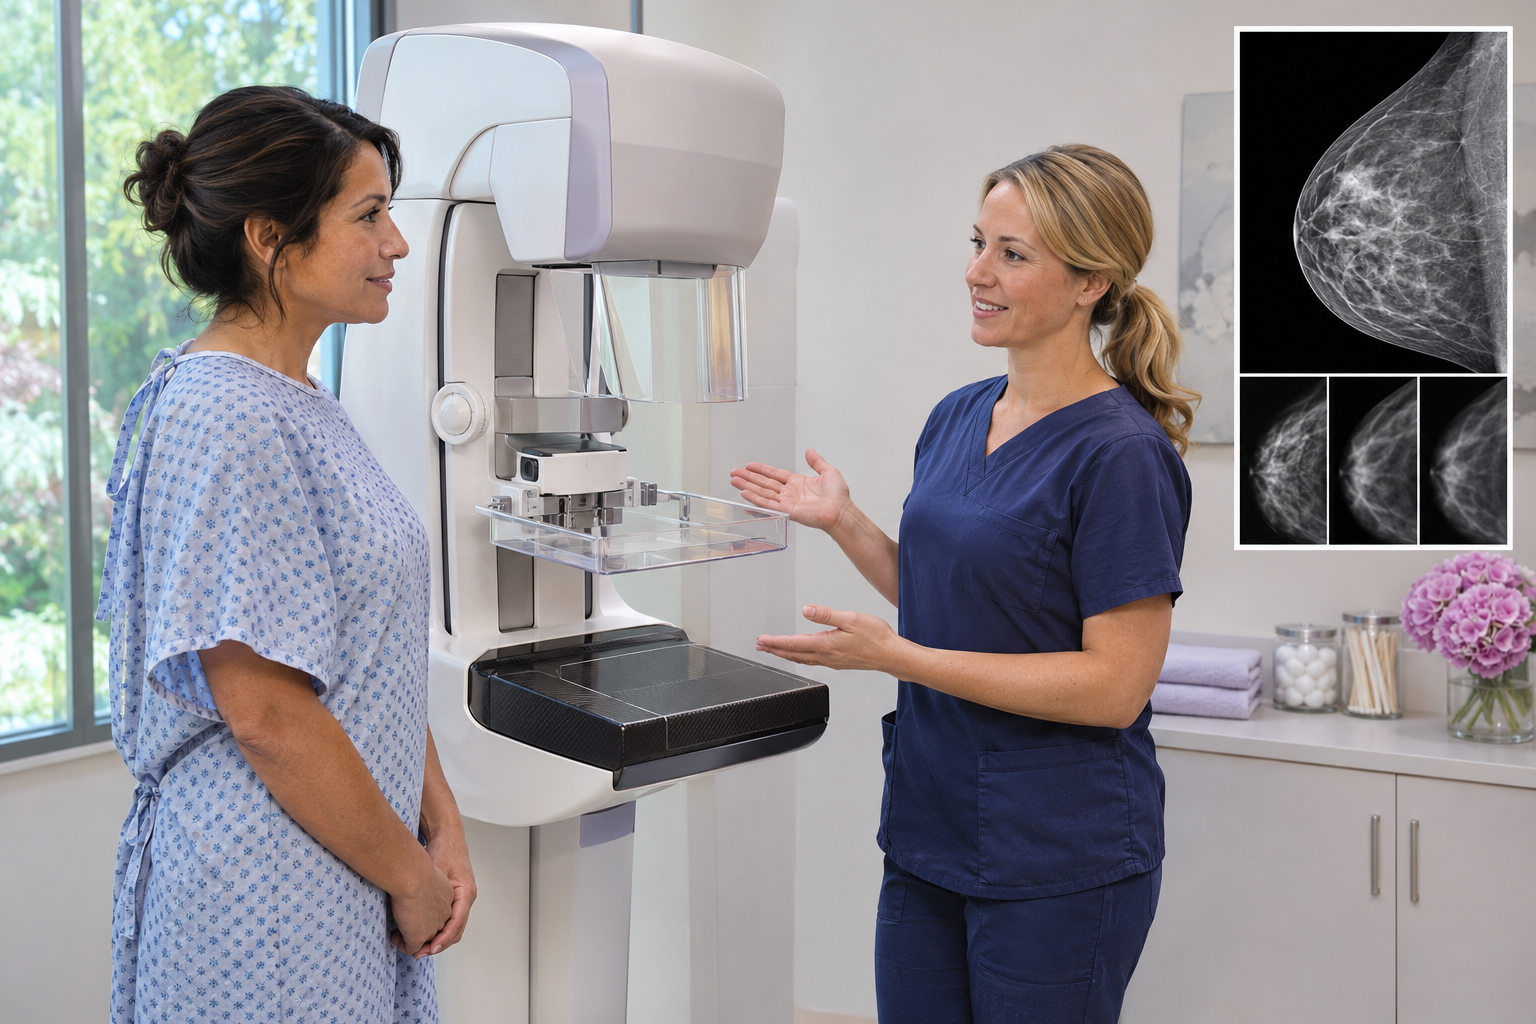
\includegraphics[width=\textwidth,keepaspectratio]{modalities/infographics/mammography_realistic.png}
\end{center}
\begin{center}\footnotesize Breast compression spreads tissue for low-dose X-ray projections; tomosynthesis reconstructs thin sections to reduce the effect of overlapping tissue. AI-generated illustration; mammogram inset is not a patient study.\end{center}

\section{Overview}
Digital mammography depicts masses, calcifications, and changes in the arrangement of breast tissue on low-dose X-ray projections. Digital breast tomosynthesis (DBT) reconstructs thin sections that can reveal a distortion hidden by overlapping tissue on a projection image.

\section{Where mammography is used}
The 80 entries include diseases, visible findings, and anatomical variants. Several share an appearance. For example, an irregular mass with radiating lines may represent invasive cancer, a radial scar, or a postoperative scar. Its location, prior images, and, when indicated, tissue sampling help establish the cause.

\subsection{Malignant breast diseases}
\begin{enumerate}[leftmargin=*,itemsep=0.45em,topsep=0.4em]
\item \textbf{Breast angiosarcoma.}\par\noindent\textbf{Symptoms:} A growing breast mass, skin discoloration, or a mass arising after breast irradiation may prompt diagnostic imaging.\par\noindent\textbf{Clinical Features:} A new mass or focal asymmetry; mammographic appearances are often nonspecific.\par\noindent\textbf{Role and sufficiency:} Mammography can localize the abnormality but cannot identify vascular histology; ultrasound/MRI and core biopsy are needed, and a negative mammogram does not exclude a clinically evident lesion.
\item \textbf{Carcinoma with medullary features.}\par\noindent\textbf{Symptoms:} A that can be felt rapidly growing mass or screening abnormality may prompt diagnostic views.\par\noindent\textbf{Clinical Features:} A round or oval high-density mass, sometimes circumscribed despite malignancy.\par\noindent\textbf{Role and sufficiency:} Imaging raises or lowers suspicion but cannot establish medullary shape; tissue diagnosis is required.
\item \textbf{Ductal carcinoma in situ (DCIS).}\par\noindent\textbf{Symptoms:} Screening commonly detects nonthat can be felt calcifications before symptoms develop.\par\noindent\textbf{Clinical Features:} Fine pleomorphic or fine linear/branching calcifications, particularly in a segmental or linear distribution; assess extent on magnification views.\par\noindent\textbf{Role and sufficiency:} Mammography is the principal detection method for calcified DCIS, but biopsy is required; noncalcified DCIS can be occult, and MRI may help assess extent in selected cases.
\item \textbf{Inflammatory breast cancer.}\par\noindent\textbf{Symptoms:} Rapid diffuse redness, edema, peau d'orange, or breast enlargement may prompt urgent diagnostic imaging.\par\noindent\textbf{Clinical Features:} Skin and trabecular thickening, increased density, asymmetry, and possible mass or abnormal nodes.\par\noindent\textbf{Role and sufficiency:} Findings overlap with mastitis and a discrete mass may be absent; clinical course and skin/core biopsy establish diagnosis, so a negative mammogram must not delay evaluation.
\item \textbf{Invasive carcinoma of no special type (invasive ductal carcinoma).}\par\noindent\textbf{Symptoms:} A screening recall, new lump, or focal symptom may lead to diagnostic mammography.\par\noindent\textbf{Clinical Features:} Irregular high-density mass, with thin lines radiating from its edge margins, architectural distortion, or suspicious calcifications; compare with prior studies.\par\noindent\textbf{Role and sufficiency:} Mammography detects and maps many lesions but cannot distinguish cancer from all scars or benign mimics; targeted ultrasound and image-guided biopsy establish diagnosis.
\item \textbf{Invasive lobular carcinoma.}\par\noindent\textbf{Symptoms:} A subtle that can be felt thickening, asymmetry, or screening change may prompt diagnostic mammography, often with DBT.\par\noindent\textbf{Clinical Features:} Architectural distortion, developing asymmetry, or subtle ill-defined density; bilateral comparison is useful.\par\noindent\textbf{Role and sufficiency:} This tumor may be mammographically occult or underestimated; targeted ultrasound and MRI are often used to define extent, while biopsy confirms it.
\item \textbf{Malignant phyllodes tumor.}\par\noindent\textbf{Symptoms:} A rapidly enlarging that can be felt mass may prompt diagnostic imaging.\par\noindent\textbf{Clinical Features:} A large oval or lobulated mass, sometimes with clefts or heterogeneous density.\par\noindent\textbf{Role and sufficiency:} Imaging cannot reliably distinguish benign, borderline, and malignant phyllodes tumors; core or excision pathology determines grade.
\item \textbf{Metaplastic breast carcinoma.}\par\noindent\textbf{Symptoms:} A rapidly enlarging that can be felt mass may prompt diagnostic mammography and ultrasound.\par\noindent\textbf{Clinical Features:} A dense irregular or occasionally circumscribed mass, with possible necrotic or cystic components on ultrasound.\par\noindent\textbf{Role and sufficiency:} Appearance is variable and may mimic benign disease; biopsy is necessary to identify metaplastic differentiation.
\item \textbf{Metastases to the breast.}\par\noindent\textbf{Symptoms:} A new breast lump in a patient with known extramammary cancer may prompt targeted imaging.\par\noindent\textbf{Clinical Features:} One or multiple round or oval masses, often without the spiculation or calcifications of a primary breast cancer.\par\noindent\textbf{Role and sufficiency:} Appearance cannot reliably determine origin; comparison with cancer history and tissue sampling are needed, with systemic staging guided by the primary disease.
\item \textbf{Mucinous carcinoma.}\par\noindent\textbf{Symptoms:} A that can be felt lump or screening-detected mass may prompt diagnostic views.\par\noindent\textbf{Clinical Features:} A lobulated, sometimes circumscribed mass; calcifications are less typical.\par\noindent\textbf{Role and sufficiency:} A deceptively circumscribed margin does not exclude cancer, and mammography cannot identify mucinous histology; biopsy is required.
\item \textbf{Paget disease of the breast.}\par\noindent\textbf{Symptoms:} Persistent unilateral nipple eczema, scaling, erosion, or discharge prompts evaluation for underlying carcinoma.\par\noindent\textbf{Clinical Features:} Nipple-areolar thickening or retraction, behind the nipple mass, and suspicious calcifications.\par\noindent\textbf{Role and sufficiency:} Mammography can identify associated disease but may be normal; persistent nipple changes require clinical assessment and skin biopsy, with ultrasound/MRI as indicated.
\item \textbf{Papillary carcinoma.}\par\noindent\textbf{Symptoms:} A that can be felt behind the nipple mass or bloody nipple discharge may prompt diagnostic mammography.\par\noindent\textbf{Clinical Features:} A circumscribed or irregular mass, asymmetry, or associated calcifications.\par\noindent\textbf{Role and sufficiency:} Imaging cannot reliably separate benign papilloma from papillary carcinoma or define subtype; targeted ultrasound and tissue sampling are required.
\item \textbf{Primary breast lymphoma.}\par\noindent\textbf{Symptoms:} A rapidly enlarging breast mass or unexplained breast asymmetry may prompt diagnostic imaging, especially with known lymphoma.\par\noindent\textbf{Clinical Features:} A dense, often noncalcified mass or diffuse asymmetry; nodal findings may coexist.\par\noindent\textbf{Role and sufficiency:} Mammography is nonspecific and cannot establish lymphoma or whether it is primary; biopsy with immunophenotyping and systemic staging are essential.
\item \textbf{Tubular carcinoma.}\par\noindent\textbf{Symptoms:} A small screening-detected distortion or mass may prompt diagnostic magnification views and DBT.\par\noindent\textbf{Clinical Features:} A small with thin lines radiating from its edge lesion, sometimes with architectural distortion.\par\noindent\textbf{Role and sufficiency:} It can resemble radial scar or other invasive cancer; biopsy is required for histology and imaging alone cannot determine subtype.
\end{enumerate}

\subsection{High-risk lesions and benign mimics}
\begin{enumerate}[leftmargin=*,itemsep=0.45em,topsep=0.4em]
\item \textbf{Atypical ductal hyperplasia (ADH).}\par\noindent\textbf{Symptoms:} Screening-detected calcifications or a mammographic target may prompt stereotactic biopsy.\par\noindent\textbf{Clinical Features:} Grouped calcifications, often amorphous or fine pleomorphic; ADH itself is a microscopic biopsy diagnosis.\par\noindent\textbf{Role and sufficiency:} Mammography identifies the target but cannot diagnose ADH or reliably separate it from DCIS; pathology and imaging--pathology concordance guide management.
\item \textbf{Atypical lobular hyperplasia (ALH).}\par\noindent\textbf{Symptoms:} Imaging is usually obtained for a separate screening or diagnostic finding, with ALH discovered on biopsy.\par\noindent\textbf{Clinical Features:} Assess whether the mammographic target is fully sampled and whether the imaging abnormality persists.\par\noindent\textbf{Role and sufficiency:} ALH has no specific mammographic appearance; imaging cannot diagnose it, and management depends on pathology, concordance, and risk context.
\item \textbf{Complex sclerosing lesion.}\par\noindent\textbf{Symptoms:} A screening distortion or suspicious asymmetry may prompt diagnostic views and biopsy.\par\noindent\textbf{Clinical Features:} Stellate architectural distortion with radiating lines, sometimes without a central mass.\par\noindent\textbf{Role and sufficiency:} It can mimic invasive carcinoma and imaging cannot distinguish them; core sampling and concordance are needed, with excision considered according to pathology and sampling adequacy.
\item \textbf{Flat epithelial atypia.}\par\noindent\textbf{Symptoms:} Grouped calcifications found at screening may be sampled stereotactically.\par\noindent\textbf{Clinical Features:} The shape and distribution of calcifications that define the biopsy target; the epithelial atypia is not visible on the image.\par\noindent\textbf{Role and sufficiency:} Mammography detects the target but cannot identify flat epithelial atypia; tissue results and concordance determine whether further sampling is warranted.
\item \textbf{Lobular carcinoma in situ (LCIS).}\par\noindent\textbf{Symptoms:} Imaging is performed for a screening abnormality or risk-based surveillance, with classic LCIS often an incidental biopsy finding.\par\noindent\textbf{Clinical Features:} Pleomorphic or florid LCIS may be associated with suspicious calcifications; classic LCIS often has no imaging correlate.\par\noindent\textbf{Role and sufficiency:} Mammography cannot diagnose LCIS; biopsy subtype, extent, and concordance determine management.
\item \textbf{Papilloma with atypia.}\par\noindent\textbf{Symptoms:} A mass, asymmetry, calcifications, or pathologic nipple discharge may prompt diagnostic imaging and biopsy.\par\noindent\textbf{Clinical Features:} A behind the nipple mass or duct-related abnormality; calcifications may also be present.\par\noindent\textbf{Role and sufficiency:} Mammography cannot detect the atypia or reliably separate papilloma from carcinoma; ultrasound and tissue sampling are needed.
\item \textbf{Radial scar.}\par\noindent\textbf{Symptoms:} A screening-detected distortion or with thin lines radiating from its edge lesion may prompt additional views, DBT, and biopsy.\par\noindent\textbf{Clinical Features:} Radiating lines converging toward a central lucency or density, often without a discrete mass.\par\noindent\textbf{Role and sufficiency:} The appearance overlaps with carcinoma; biopsy establishes the lesion and associated atypia, with management based on radiology-pathology concordance.
\end{enumerate}

\subsection{Benign breast tumors and masses}
\begin{enumerate}[leftmargin=*,itemsep=0.45em,topsep=0.4em]
\item \textbf{Benign adenomyoepithelioma.}\par\noindent\textbf{Symptoms:} A that can be felt lump or screening-detected mass may prompt diagnostic views.\par\noindent\textbf{Clinical Features:} An oval, lobulated, or irregular mass, with margins and interval growth carefully assessed.\par\noindent\textbf{Role and sufficiency:} Appearance overlaps with malignant and other benign tumors; biopsy is needed to distinguish benign, atypical, and malignant forms.
\item \textbf{Benign phyllodes tumor.}\par\noindent\textbf{Symptoms:} A rapidly enlarging that can be felt mass may prompt diagnostic imaging.\par\noindent\textbf{Clinical Features:} A circumscribed, often lobulated mass that may be large and heterogeneous.\par\noindent\textbf{Role and sufficiency:} Mammography cannot reliably separate phyllodes tumor from fibroadenoma or determine grade; tissue diagnosis is needed.
\item \textbf{Breast hamartoma.}\par\noindent\textbf{Symptoms:} A that can be felt lump or screening asymmetry may prompt mammography.\par\noindent\textbf{Clinical Features:} A circumscribed mass containing mixed fat and fibroglandular tissue, sometimes with a thin pseudocapsule.\par\noindent\textbf{Role and sufficiency:} A classic appearance can be diagnostic, but atypical or changing lesions require targeted ultrasound and sometimes biopsy.
\item \textbf{Breast hemangioma.}\par\noindent\textbf{Symptoms:} A that can be felt or incidental mass may prompt diagnostic imaging.\par\noindent\textbf{Clinical Features:} A circumscribed mass, sometimes with calcifications, without a reliably specific pattern.\par\noindent\textbf{Role and sufficiency:} Mammography cannot establish vascular histology; ultrasound/Doppler and, when needed, biopsy characterize an indeterminate lesion.
\item \textbf{Breast lipoma.}\par\noindent\textbf{Symptoms:} A that can be felt soft mass or incidental lesion may be assessed on mammography.\par\noindent\textbf{Clinical Features:} A circumscribed radiolucent mass with a thin capsule and no suspicious solid component.\par\noindent\textbf{Role and sufficiency:} A classic fat-containing appearance is usually sufficient; atypical density or discordant examination warrants further imaging.
\item \textbf{Breast myofibroblastoma.}\par\noindent\textbf{Symptoms:} A slowly growing that can be felt mass may prompt diagnostic mammography.\par\noindent\textbf{Clinical Features:} A circumscribed or mildly lobulated soft-tissue density, sometimes with coarse calcification.\par\noindent\textbf{Role and sufficiency:} The appearance is nonspecific and cannot identify this stromal tumor; core biopsy establishes the diagnosis.
\item \textbf{Fibroadenoma.}\par\noindent\textbf{Symptoms:} A that can be felt lump or screening-detected mass may lead to diagnostic assessment, especially in older patients.\par\noindent\textbf{Clinical Features:} An oval or gently lobulated circumscribed mass; involution may produce coarse popcorn-like calcification.\par\noindent\textbf{Role and sufficiency:} A stable classic lesion may be characterized with ultrasound and prior comparison, but mammography alone cannot prove fibroadenoma when features are new or suspicious.
\item \textbf{Granular cell tumor.}\par\noindent\textbf{Symptoms:} A firm that can be felt lump or imaging abnormality may prompt diagnostic views.\par\noindent\textbf{Clinical Features:} An irregular mass or architectural distortion, sometimes with thin lines radiating from its edge and indistinguishable from cancer.\par\noindent\textbf{Role and sufficiency:} Imaging cannot distinguish this benign tumor from carcinoma; biopsy is required.
\item \textbf{Intraductal papilloma.}\par\noindent\textbf{Symptoms:} Bloody nipple discharge or a behind the nipple lump may prompt diagnostic mammography and targeted ultrasound.\par\noindent\textbf{Clinical Features:} A behind the nipple mass, focal asymmetry, or duct-associated calcifications; small papillomas may be occult.\par\noindent\textbf{Role and sufficiency:} Mammography may miss the lesion and cannot determine atypia; ultrasound, duct evaluation, and tissue sampling are considered based on symptoms and findings.
\item \textbf{Involuting fibroadenoma.}\par\noindent\textbf{Symptoms:} Screening or follow-up may show progressive calcification within a known mass.\par\noindent\textbf{Clinical Features:} Coarse, dense, popcorn-like calcifications developing within a circumscribed lesion.\par\noindent\textbf{Role and sufficiency:} A classic evolution is benign and often needs no biopsy; suspicious shape or discordant change requires diagnostic assessment.
\item \textbf{Pseudoangiomatous stromal hyperplasia (PASH).}\par\noindent\textbf{Symptoms:} A that can be felt enlarging mass or screening asymmetry may prompt diagnostic imaging.\par\noindent\textbf{Clinical Features:} A circumscribed mass or focal asymmetry; microscopic PASH may have no visible correlate.\par\noindent\textbf{Role and sufficiency:} Imaging is nonspecific and cannot establish PASH; core biopsy and concordance determine whether the result explains the finding.
\item \textbf{Tubular adenoma.}\par\noindent\textbf{Symptoms:} A that can be felt lump or screening mass may prompt diagnostic views.\par\noindent\textbf{Clinical Features:} A circumscribed, often oval mass; calcifications may occur.\par\noindent\textbf{Role and sufficiency:} Its appearance overlaps with fibroadenoma and other lesions; biopsy is needed when imaging is not characteristically benign.
\end{enumerate}

\subsection{Cystic and fibrocystic breast conditions}
\begin{enumerate}[leftmargin=*,itemsep=0.45em,topsep=0.4em]
\item \textbf{Apocrine metaplasia.}\par\noindent\textbf{Symptoms:} Imaging may be obtained for a cyst, calcifications, or that can be felt finding, with apocrine change identified incidentally on pathology.\par\noindent\textbf{Clinical Features:} Describe the associated cystic lesion or calcification pattern; apocrine metaplasia has no specific mammographic sign.\par\noindent\textbf{Role and sufficiency:} Mammography cannot diagnose the microscopic change; pathology and concordance determine whether it explains the target.
\item \textbf{Breast adenosis.}\par\noindent\textbf{Symptoms:} A screening asymmetry, mass, or calcification may prompt diagnostic assessment.\par\noindent\textbf{Clinical Features:} Focal asymmetry, small masses, or calcifications, which vary with the subtype.\par\noindent\textbf{Role and sufficiency:} These findings are nonspecific and can mimic malignancy; targeted ultrasound and biopsy are used when suspicious, while pathology identifies adenosis.
\item \textbf{Complicated breast cyst.}\par\noindent\textbf{Symptoms:} A that can be felt lump or circumscribed mammographic mass may prompt targeted ultrasound.\par\noindent\textbf{Clinical Features:} On mammography, a round or oval circumscribed mass; ultrasound assesses mobile debris, wall features, and whether a solid component exists.\par\noindent\textbf{Role and sufficiency:} Mammography cannot reliably distinguish a complicated cyst from a solid mass; ultrasound is the key characterization test and suspicious solid components may require biopsy.
\item \textbf{Fibrocystic breast changes.}\par\noindent\textbf{Symptoms:} Cyclic nodularity, focal pain, or screening abnormalities may prompt diagnostic imaging.\par\noindent\textbf{Clinical Features:} Multiple circumscribed masses, focal asymmetries, or calcifications; evaluate each dominant or new finding rather than attributing all changes to a general pattern.\par\noindent\textbf{Role and sufficiency:} Mammography describes visible findings but does not establish a single fibrocystic diagnosis or dismiss a suspicious focal lesion; ultrasound may clarify cystic masses.
\item \textbf{Galactocele.}\par\noindent\textbf{Symptoms:} A persistent lump during lactation or after weaning may prompt imaging.\par\noindent\textbf{Clinical Features:} A circumscribed mass with a fat-fluid level when visible, correlating with lactation history.\par\noindent\textbf{Role and sufficiency:} This appearance can be characteristic, but ultrasound is often preferred during lactation and evaluates internal contents; atypical or persistent lesions need further assessment.
\item \textbf{Oil cyst.}\par\noindent\textbf{Symptoms:} A that can be felt lump after surgery, trauma, or fat grafting may prompt diagnostic views.\par\noindent\textbf{Clinical Features:} A fat-density round mass, sometimes with a thin rim of calcification.\par\noindent\textbf{Role and sufficiency:} A classic oil cyst is a benign imaging diagnosis; irregular margins or an unexplained that can be felt abnormality require ultrasound and possible biopsy.
\item \textbf{Sclerosing adenosis.}\par\noindent\textbf{Symptoms:} Screening calcifications, a mass, or distortion may lead to diagnostic imaging and biopsy.\par\noindent\textbf{Clinical Features:} Grouped calcifications, focal asymmetry, or architectural distortion.\par\noindent\textbf{Role and sufficiency:} It can closely mimic carcinoma; imaging cannot confirm sclerosing adenosis, and tissue diagnosis with concordance is needed for suspicious findings.
\item \textbf{Simple breast cyst.}\par\noindent\textbf{Symptoms:} A that can be felt lump or screening-detected circumscribed mass may prompt diagnostic assessment.\par\noindent\textbf{Clinical Features:} A round or oval circumscribed mass; targeted ultrasound demonstrates a thin wall and anechoic fluid with posterior enhancement.\par\noindent\textbf{Role and sufficiency:} Mammography alone cannot prove simple fluid; a classic ultrasound appearance is generally sufficient, while complex features prompt further evaluation.
\end{enumerate}

Debris can move within a complicated cyst. A discrete solid component on ultrasound raises a different diagnostic question and is described as part of a complex cystic and solid mass.

\subsection{Inflammatory and infectious conditions}
\begin{enumerate}[leftmargin=*,itemsep=0.45em,topsep=0.4em]
\item \textbf{Breast abscess.}\par\noindent\textbf{Symptoms:} A painful red swelling or persistent focal lump may prompt imaging, particularly if the patient is outside the usual lactational setting or does not improve.\par\noindent\textbf{Clinical Features:} Focal asymmetry, skin thickening, and surrounding edema; targeted ultrasound identifies a drainable complex collection.\par\noindent\textbf{Role and sufficiency:} Mammography cannot reliably separate abscess from inflammatory cancer; ultrasound and clinical assessment guide drainage, with biopsy or reassessment for persistent abnormalities.
\item \textbf{Breast edema.}\par\noindent\textbf{Symptoms:} Diffuse swelling, peau d'orange, or skin thickening may prompt diagnostic views to assess extent and associated lesion.\par\noindent\textbf{Clinical Features:} Skin and trabecular thickening, increased density, and asymmetry compared with prior images.\par\noindent\textbf{Role and sufficiency:} These signs are nonspecific and occur with infection, treatment, heart failure, or lymphatic obstruction; clinical context and targeted imaging determine cause.
\item \textbf{Breast tuberculosis.}\par\noindent\textbf{Symptoms:} A chronic lump, sinus, or skin change in an appropriate epidemiologic context may prompt imaging.\par\noindent\textbf{Clinical Features:} Irregular mass, asymmetry, skin thickening, or abnormal nodes; none is specific for tuberculosis.\par\noindent\textbf{Role and sufficiency:} Mammography cannot identify the organism or reliably distinguish cancer; tissue sampling for histology and microbiology is required.
\item \textbf{Diabetic mastopathy.}\par\noindent\textbf{Symptoms:} A firm that can be felt mass in a person with long-standing diabetes may prompt diagnostic imaging.\par\noindent\textbf{Clinical Features:} Dense tissue, focal asymmetry, or an irregular mass; the lesion may also be occult.\par\noindent\textbf{Role and sufficiency:} Imaging can mimic carcinoma and diabetes does not explain away suspicious features; ultrasound-guided core biopsy is often needed for a new indeterminate mass.
\item \textbf{Granulomatous mastitis.}\par\noindent\textbf{Symptoms:} Painful mass, erythema, or recurrent inflammatory change may prompt imaging when symptoms persist or are atypical.\par\noindent\textbf{Clinical Features:} Asymmetry, irregular masses, skin thickening, or sinus-related changes.\par\noindent\textbf{Role and sufficiency:} Findings can resemble invasive cancer or infection; biopsy and microbiological assessment help establish cause, and follow-up confirms resolution.
\item \textbf{Mammary duct ectasia.}\par\noindent\textbf{Symptoms:} Nipple discharge, behind the nipple discomfort, or a subareolar lump may prompt diagnostic imaging.\par\noindent\textbf{Clinical Features:} Dilated behind the nipple ducts and smooth large rod-like secretory calcifications.\par\noindent\textbf{Role and sufficiency:} Mammography can show duct-related calcifications, but ultrasound better evaluates duct contents; suspicious discharge or intraductal mass needs targeted workup.
\item \textbf{Mastitis.}\par\noindent\textbf{Symptoms:} Persistent focal inflammation, a mass, or failure to improve with treatment may prompt imaging to look for an abscess or alternate diagnosis.\par\noindent\textbf{Clinical Features:} Skin/trabecular thickening, increased density, and focal asymmetry.\par\noindent\textbf{Role and sufficiency:} These are nonspecific and do not distinguish infection from inflammatory cancer; ultrasound evaluates a collection, and persistent change requires reassessment and possible biopsy.
\item \textbf{Periductal mastitis.}\par\noindent\textbf{Symptoms:} Recurrent subareolar pain, discharge, or inflammation may prompt diagnostic assessment.\par\noindent\textbf{Clinical Features:} Retroareolar asymmetry, duct widening, or associated mass; compare with the symptomatic side and prior studies.\par\noindent\textbf{Role and sufficiency:} Mammography is not specific for periductal inflammation; targeted ultrasound and clinical follow-up assess abscess or an alternative lesion.
\end{enumerate}

\subsection{Traumatic and postoperative conditions}
\begin{enumerate}[leftmargin=*,itemsep=0.45em,topsep=0.4em]
\item \textbf{Breast hematoma.}\par\noindent\textbf{Symptoms:} A new lump or bruising after trauma, biopsy, or surgery may prompt diagnostic imaging.\par\noindent\textbf{Clinical Features:} A focal mass or asymmetry and its evolution on prior or follow-up studies; ultrasound can show evolving internal echoes.\par\noindent\textbf{Role and sufficiency:} A resolving appearance supports hematoma, but a persistent or enlarging mass needs further evaluation because bleeding can obscure an underlying lesion.
\item \textbf{Extracapsular silicone implant rupture.}\par\noindent\textbf{Symptoms:} Pain, change in implant contour, or concern for implant complication may prompt imaging.\par\noindent\textbf{Clinical Features:} Silicone outside the implant capsule, sometimes as dense deposits in breast tissue or nodes.\par\noindent\textbf{Role and sufficiency:} Mammography may show extracapsular silicone but is insensitive for intracapsular rupture; implant-protocol MRI or ultrasound is preferred to assess integrity.
\item \textbf{Fat necrosis.}\par\noindent\textbf{Symptoms:} A that can be felt lump after surgery, trauma, or radiation may prompt diagnostic views.\par\noindent\textbf{Clinical Features:} Oil cyst, fat-containing mass, or thin rim calcification; irregular spiculation or evolving distortion is less reassuring.\par\noindent\textbf{Role and sufficiency:} Classic fat-containing findings can establish a benign explanation, but suspicious or discordant lesions require biopsy because fat necrosis can mimic cancer.
\item \textbf{Postoperative scarring.}\par\noindent\textbf{Symptoms:} Surveillance or a new that can be felt finding after breast surgery may prompt comparison with baseline postoperative studies.\par\noindent\textbf{Clinical Features:} Distortion at the operative bed and whether it remains stable or becomes more conspicuous.\par\noindent\textbf{Role and sufficiency:} Stable scar is often characterized by comparison; new or progressive distortion warrants diagnostic views, ultrasound, and possible biopsy.
\item \textbf{Postoperative seroma.}\par\noindent\textbf{Symptoms:} A that can be felt swelling after surgery may prompt assessment of the operative site.\par\noindent\textbf{Clinical Features:} A circumscribed mass at the surgical bed; ultrasound determines whether it is fluid-filled.\par\noindent\textbf{Role and sufficiency:} Mammography cannot confirm fluid contents; a typical ultrasound appearance and expected clinical course may suffice, while complex or persistent findings need further workup.
\item \textbf{Radiation-induced fibrosis.}\par\noindent\textbf{Symptoms:} Follow-up after breast irradiation evaluates expected treatment change and detects recurrence.\par\noindent\textbf{Clinical Features:} Late volume loss, retraction, and stable distortion; early skin/trabecular thickening can reflect edema.\par\noindent\textbf{Role and sufficiency:} Stability over serial examinations supports fibrosis, but new or progressive change requires targeted evaluation and sometimes biopsy.
\item \textbf{Silicone granuloma.}\par\noindent\textbf{Symptoms:} A that can be felt nodule or abnormal node in a patient with silicone implants may prompt diagnostic imaging.\par\noindent\textbf{Clinical Features:} Dense silicone deposits or nodules, including within regional lymph nodes.\par\noindent\textbf{Role and sufficiency:} Mammography can locate deposits but cannot confirm the granulomatous reaction or exclude malignancy; ultrasound/MRI and biopsy are used for indeterminate lesions.
\end{enumerate}

\subsection{Breast calcification patterns}
Describe both the shape of individual deposits and the distribution of the group. For example, fine pleomorphic deposits in a segmental distribution raise concern for a ductal process.

\begin{enumerate}[leftmargin=*,itemsep=0.45em,topsep=0.4em]
\item \textbf{Amorphous calcifications.}\par\noindent\textbf{Symptoms:} Screening detects calcifications that require diagnostic magnification views to characterize.\par\noindent\textbf{Clinical Features:} Tiny hazy particles whose shape is indistinct; document whether grouped, regional, linear, or segmental.\par\noindent\textbf{Role and sufficiency:} Distribution and comparison guide BI-RADS assessment, but suspicious grouped patterns generally require stereotactic biopsy; shape alone does not identify histology.
\item \textbf{Coarse calcifications.}\par\noindent\textbf{Symptoms:} A screening calcification cluster may prompt magnification views to determine whether deposits are characteristically benign.\par\noindent\textbf{Clinical Features:} Large, dense, often confluent deposits, including popcorn-like calcification in an involuting fibroadenoma or dystrophic calcification after injury.\par\noindent\textbf{Role and sufficiency:} A classic benign pattern is usually sufficient for benign classification; atypical shape or distribution may require additional assessment.
\item \textbf{Coarse heterogeneous calcifications.}\par\noindent\textbf{Symptoms:} Newly detected calcifications are characterized with magnification views and comparison.\par\noindent\textbf{Clinical Features:} Irregular, conspicuous particles with variable shape, typically smaller and less uniformly benign than coarse dystrophic deposits; assess distribution.\par\noindent\textbf{Role and sufficiency:} Suspicion depends on the group and context; mammography determines whether biopsy is warranted but cannot determine pathology.
\item \textbf{Fine linear or fine linear-branching calcifications.}\par\noindent\textbf{Symptoms:} Screening or diagnostic imaging detects a potentially ductal calcification pattern requiring workup.\par\noindent\textbf{Clinical Features:} Thin, irregular, discontinuous or branching deposits; map their linear or segmental distribution and extent.\par\noindent\textbf{Role and sufficiency:} This shape is suspicious and commonly prompts image-guided biopsy; mammography cannot establish DCIS or invasive disease.
\item \textbf{Fine pleomorphic calcifications.}\par\noindent\textbf{Symptoms:} Screening-detected calcifications are magnified to assess shape and distribution.\par\noindent\textbf{Clinical Features:} Small irregular particles varying in shape and size, with grouped, linear, or segmental arrangement recorded.\par\noindent\textbf{Role and sufficiency:} A suspicious pattern often requires stereotactic biopsy; image appearance estimates risk but does not provide tissue diagnosis.
\item \textbf{Large rod-like calcifications.}\par\noindent\textbf{Symptoms:} Nipple discharge or incidental ductal calcifications may prompt diagnostic review.\par\noindent\textbf{Clinical Features:} Smooth, elongated calcifications following a duct, often with a central lucency and behind the nipple predominance.\par\noindent\textbf{Role and sufficiency:} A classic bilateral secretory pattern is benign; unilateral, irregular, or associated mass findings require further evaluation.
\item \textbf{Layering calcifications (milk of calcium).}\par\noindent\textbf{Symptoms:} Indeterminate round calcifications may prompt magnification views, including a true lateral projection.\par\noindent\textbf{Clinical Features:} Dependent sediment in microcysts forming a crescent or teacup shape on the lateral view.\par\noindent\textbf{Role and sufficiency:} Demonstrated layering is a characteristic benign feature and can avoid biopsy; if layering is absent or shape remains suspicious, further assessment is needed.
\item \textbf{Rim calcifications.}\par\noindent\textbf{Symptoms:} A mass with peripheral calcification may be evaluated after trauma, surgery, or on screening.\par\noindent\textbf{Clinical Features:} Thin, smooth eggshell-like calcium outlining an oil cyst or other fat-containing lesion.\par\noindent\textbf{Role and sufficiency:} A classic rim pattern is benign; thick, irregular, or incomplete calcification around a suspicious mass should not be assumed benign.
\item \textbf{Skin calcifications.}\par\noindent\textbf{Symptoms:} Superficial calcifications may be recalled when their location is uncertain on standard views.\par\noindent\textbf{Clinical Features:} Deposits with central lucency; a tangential skin marker/view confirms superficial location.\par\noindent\textbf{Role and sufficiency:} Once confirmed as dermal, they are benign; without localization, they can be confused with intraparenchymal calcifications.
\item \textbf{Suture calcifications.}\par\noindent\textbf{Symptoms:} Calcifications near a surgical bed may prompt comparison with operative history and prior images.\par\noindent\textbf{Clinical Features:} Linear or knot-shaped deposits along a suture track, typically within a stable scar.\par\noindent\textbf{Role and sufficiency:} A typical postoperative pattern can be recognized on mammography; new suspicious calcifications outside the expected operative site need separate assessment.
\item \textbf{Vascular calcifications.}\par\noindent\textbf{Symptoms:} These are usually incidental findings on screening or diagnostic mammography.\par\noindent\textbf{Clinical Features:} Parallel, rail-like calcification along arterial walls rather than clustered ductal deposits.\par\noindent\textbf{Role and sufficiency:} Mammography readily identifies the vascular pattern but does not diagnose coronary artery disease; cardiovascular risk assessment is a separate clinical decision.
\end{enumerate}

\subsection{Structural findings and anatomical variants}
BI-RADS v2025 describes an asymmetry by its appearance on the current examination. Report separately whether it is new, larger, or more conspicuous on comparison with prior mammograms. An interval increase can warrant further assessment.
\begin{enumerate}[leftmargin=*,itemsep=0.45em,topsep=0.4em]
\item \textbf{Accessory breast tissue.}\par\noindent\textbf{Symptoms:} An axillary lump or focal swelling may prompt imaging to determine whether it is breast tissue or another lesion.\par\noindent\textbf{Clinical Features:} Fibroglandular tissue separate from the main breast, often in the axilla; the normal axillary tail remains continuous with breast tissue.\par\noindent\textbf{Role and sufficiency:} A characteristic appearance may establish ectopic tissue, but a discrete mass within it requires standard diagnostic evaluation.
\item \textbf{Architectural distortion.}\par\noindent\textbf{Symptoms:} Screening recall or a that can be felt thickening may prompt spot compression and DBT.\par\noindent\textbf{Clinical Features:} Converging lines or focal retraction without a definite mass, persistence across projections, and interval development.\par\noindent\textbf{Role and sufficiency:} DBT improves conspicuity but distortion is not a diagnosis; targeted ultrasound and biopsy are often needed to distinguish cancer from scar or radial scar.
\item \textbf{Asymmetry on one projection.}\par\noindent\textbf{Symptoms:} A density seen on only one screening view triggers recall to determine whether it represents overlap or a true lesion.\par\noindent\textbf{Clinical Features:} Whether the density persists on a second projection, spot compression, or DBT and whether it has a mass-like margin.\par\noindent\textbf{Role and sufficiency:} Additional views resolve many summation artifacts; persistent findings require targeted ultrasound or biopsy depending on appearance.
\item \textbf{Axillary lymphadenopathy.}\par\noindent\textbf{Symptoms:} A that can be felt axillary node, screening finding, or known cancer may prompt evaluation of regional nodes.\par\noindent\textbf{Clinical Features:} Enlargement, round shape, cortical thickening, and loss or displacement of the fatty hilum.\par\noindent\textbf{Role and sufficiency:} Mammography detects abnormal shape but ultrasound better evaluates cortex and guides sampling; imaging cannot determine benign versus malignant cause.
\item \textbf{Dense breast tissue.}\par\noindent\textbf{Symptoms:} Density is reported on routine screening because it affects masking and risk discussions.\par\noindent\textbf{Clinical Features:} Heterogeneously or extremely dense fibroglandular tissue (BI-RADS C or D) and any focal asymmetry concealed within it.\par\noindent\textbf{Role and sufficiency:} Mammography remains a screening test but sensitivity is reduced by density; supplemental imaging decisions depend on overall risk and local guidance, not density alone.
\item \textbf{Focal asymmetry.}\par\noindent\textbf{Symptoms:} A focal density on screening or a localized symptom may prompt diagnostic views.\par\noindent\textbf{Clinical Features:} Fibroglandular density occupying less than one quadrant and present on two projections; assess for interval development or associated distortion.\par\noindent\textbf{Role and sufficiency:} Stable nondeveloping asymmetry may be benign, but a new or enlarging finding warrants additional views and targeted ultrasound, with biopsy if suspicious.
\item \textbf{Global asymmetry.}\par\noindent\textbf{Symptoms:} A unilateral difference in breast size or density may prompt diagnostic comparison.\par\noindent\textbf{Clinical Features:} More fibroglandular tissue over at least one quadrant without a discrete mass, distortion, or suspicious calcifications.\par\noindent\textbf{Role and sufficiency:} A stable asymmetry without suspicious features may be a normal variant; new asymmetry or a that can be felt correlate requires targeted workup.
\item \textbf{Intramammary lymphadenopathy.}\par\noindent\textbf{Symptoms:} An incidental node or known malignancy may prompt comparison and targeted assessment.\par\noindent\textbf{Clinical Features:} Typical oval shape and preserved fatty hilum versus interval growth, roundness, or hilar loss.\par\noindent\textbf{Role and sufficiency:} A classic stable node is usually benign; suspicious shape is not specific and ultrasound-guided biopsy may be needed.
\item \textbf{Nipple retraction.}\par\noindent\textbf{Symptoms:} New unilateral inversion, discharge, or a behind the nipple lump prompts diagnostic evaluation.\par\noindent\textbf{Clinical Features:} New inward displacement, asymmetric nipple thickening, behind the nipple mass, or distortion compared with prior images.\par\noindent\textbf{Role and sufficiency:} Longstanding symmetric inversion is often benign, but new retraction can signal malignancy; mammography may be normal, so examination and targeted ultrasound are important.
\item \textbf{Skin thickening.}\par\noindent\textbf{Symptoms:} Redness, edema, peau d'orange, or post-treatment change may prompt diagnostic views.\par\noindent\textbf{Clinical Features:} Extent and asymmetry of dermal thickening, trabecular edema, and any underlying mass or distortion.\par\noindent\textbf{Role and sufficiency:} The sign is nonspecific; correlate with symptoms, treatment history, and ultrasound, and investigate persistent or progressive change for malignancy.
\end{enumerate}

\subsection{Male breast conditions}
When the physical examination is typical of gynecomastia or pseudogynecomastia, imaging is usually unnecessary. Mammography can help characterize an indeterminate or suspicious palpable abnormality.
\begin{enumerate}[leftmargin=*,itemsep=0.45em,topsep=0.4em]
\item \textbf{Gynecomastia.}\par\noindent\textbf{Symptoms:} Imaging is used when a male breast lump is indeterminate or clinically suspicious; a typical examination generally needs no imaging.\par\noindent\textbf{Clinical Features:} Flame-shaped dendritic tissue radiating from the nipple or a more nodular behind the nipple density.\par\noindent\textbf{Role and sufficiency:} A classic pattern with matching examination is usually sufficient; eccentric hard mass, nipple change, or discordance requires targeted ultrasound and possible biopsy.
\item \textbf{Male breast carcinoma.}\par\noindent\textbf{Symptoms:} A hard eccentric lump, nipple retraction, discharge, or axillary node prompts diagnostic imaging.\par\noindent\textbf{Clinical Features:} Irregular eccentric mass, architectural distortion, suspicious calcifications, or associated nipple/skin change.\par\noindent\textbf{Role and sufficiency:} Mammography localizes and characterizes but cannot confirm cancer; core biopsy is required for suspicious findings.
\item \textbf{Pseudogynecomastia.}\par\noindent\textbf{Symptoms:} Imaging may be requested when diffuse male breast enlargement is difficult to distinguish clinically from a glandular mass.\par\noindent\textbf{Clinical Features:} Predominantly fatty tissue without a discrete behind the nipple glandular density or suspicious mass.\par\noindent\textbf{Role and sufficiency:} A typical clinical/imaging pattern is usually sufficient; a focal or eccentric abnormality needs diagnostic evaluation.
\end{enumerate}

\subsection{Summary}
\begin{center}
\begin{tabular}{@{}p{0.70\textwidth}r@{}}
\toprule
\textbf{Disease category} & \textbf{Entries} \\
\midrule
Category & Conditions and findings \\
Benign tumors and masses & 12 \\
Calcification patterns & 11 \\
Cystic and fibrocystic conditions & 8 \\
High-risk lesions and benign mimics & 7 \\
Inflammatory and infectious conditions & 8 \\
Male breast conditions & 3 \\
Malignant breast diseases & 14 \\
Structural findings and anatomical variants & 10 \\
Traumatic and postoperative conditions & 7 \\
\midrule
\textbf{Total} & \textbf{80} \\
\bottomrule
\end{tabular}
\end{center}

\subsection{BI-RADS classification}
The American College of Radiology Breast Imaging Reporting and Data System (BI-RADS v2025) links the final assessment to a likelihood of malignancy. In the table, $p$ is the estimated probability for the assessed finding. A negative examination can still miss clinically evident disease.

\begin{longtable}{@{}p{0.13\textwidth}p{0.43\textwidth}p{0.38\textwidth}@{}}
\toprule
\textbf{BI-RADS} & \textbf{Interpretation} & \textbf{Probability of malignancy} \\
\midrule
\endfirsthead
\toprule
0 & Incomplete. Additional imaging or prior mammograms for comparison are needed. & Not applicable \\
\midrule
\endhead
1 & Negative & Essentially 0\% \\
2 & Benign & Essentially 0\% \\
3 & Probably benign after diagnostic evaluation. Short-interval imaging follow-up is usual. & $0 < p \leq 2\%$ \\
4A & Low suspicion & $2\% < p \leq 10\%$ \\
4B & Moderate suspicion & $10\% < p \leq 50\%$ \\
4C & High suspicion & $50\% < p < 95\%$ \\
5 & Highly suggestive of malignancy & $p \geq 95\%$ \\
6 & Known biopsy-proven malignancy & Not applicable \\
\textbf{BI-RADS} & \textbf{Interpretation} & \textbf{Probability of malignancy} \\
\bottomrule
\end{longtable}

\subsection{Published medical image datasets and sources}
\begin{longtable}{@{}p{0.34\textwidth}p{0.60\textwidth}@{}}
\toprule
\textbf{Source} & \textbf{Primary utility} \\
\midrule
\endfirsthead
\toprule
\textbf{Source} & \textbf{Primary utility} \\
\midrule
\endhead
American College of Radiology & BI-RADS and clinical imaging guidelines \\
\href{https://physionet.org/content/vindr-mammo/1.0.0/}{VinDr-Mammo} & Full-field digital mammograms with radiologists’ finding annotations, density categories, and BI-RADS assessments \\
\href{https://pubmed.ncbi.nlm.nih.gov/22078258/}{INbreast} & Full-field digital mammograms with annotated lesions \\
\href{https://wiki.cancerimagingarchive.net/pages/viewpage.action?pageId=52764371}{CBIS-DDSM} & Scanned film mammograms with annotated masses and calcifications \\
PubMed Central & Literature archive containing published mammographic images \\
Radiopaedia & Annotated clinical mammography cases \\
The Cancer Imaging Archive & Archive hosting individual cancer imaging collections \\
\bottomrule
\end{longtable}

\subsection{Annotation levels for dataset development}
Consider a group of calcifications that undergoes mammographically guided biopsy. Its record can preserve three distinct observations.
\begin{itemize}
    \item \textbf{Image finding.} Record the shape and distribution of the calcifications, their location, and the acquisition type (digitized film, full-field digital mammography, or DBT).
    \item \textbf{Imaging assessment.} Record the radiologist's BI-RADS category and the lexicon version used at interpretation. Document any mapping of older terms to v2025.
    \item \textbf{Reference diagnosis.} Link the biopsy result, such as ADH or DCIS, to the sampled calcifications and document whether it explains the imaging finding. For a benign finding established by ultrasound or follow-up, record that reference method.
\end{itemize}

\subsection{Selected clinical references}
\begin{itemize}
    \item American College of Radiology. \href{https://www.acr.org/Clinical-Resources/Clinical-Tools-and-Reference/Reporting-and-Data-Systems/BI-RADS}{BI-RADS v2025 mammography lexicon, assessment categories, and summary of changes}.
    \item National Cancer Institute. \href{https://www.cancer.gov/types/breast/breast-cancer-types/inflammatory}{Inflammatory breast cancer}, \href{https://www.cancer.gov/types/breast/breast-cancer-types/paget-disease-breast}{Paget disease of the breast}, and \href{https://www.cancer.gov/types/breast/screening/dense-breasts}{breast density}.
    \item American Society of Breast Surgeons. \href{https://www.breastsurgeons.org/docs/statements/asbrs-high-risk-lesions.pdf}{Surgical management of benign or high-risk lesions}.
    \item \href{https://pmc.ncbi.nlm.nih.gov/articles/PMC13341065/}{WHO classification of tumors of the breast, sixth edition}. \href{https://pubmed.ncbi.nlm.nih.gov/8539362/}{Mammographic and sonographic findings in benign and malignant phyllodes tumors}.
    \item \href{https://pubmed.ncbi.nlm.nih.gov/8659366/}{Serial mammographic findings after breast conservation therapy}. American College of Radiology. Appropriateness Criteria for \href{https://acsearch.acr.org/docs/3100728/Narrative}{breast implant evaluation} and \href{https://acsearch.acr.org/docs/3091547/Narrative}{evaluation of the symptomatic male breast}.
\end{itemize}

\chapter{Ultrasound}
\label{ch:ultrasound}

% Chapter-opening illustrated modality infographic.
\begin{center}
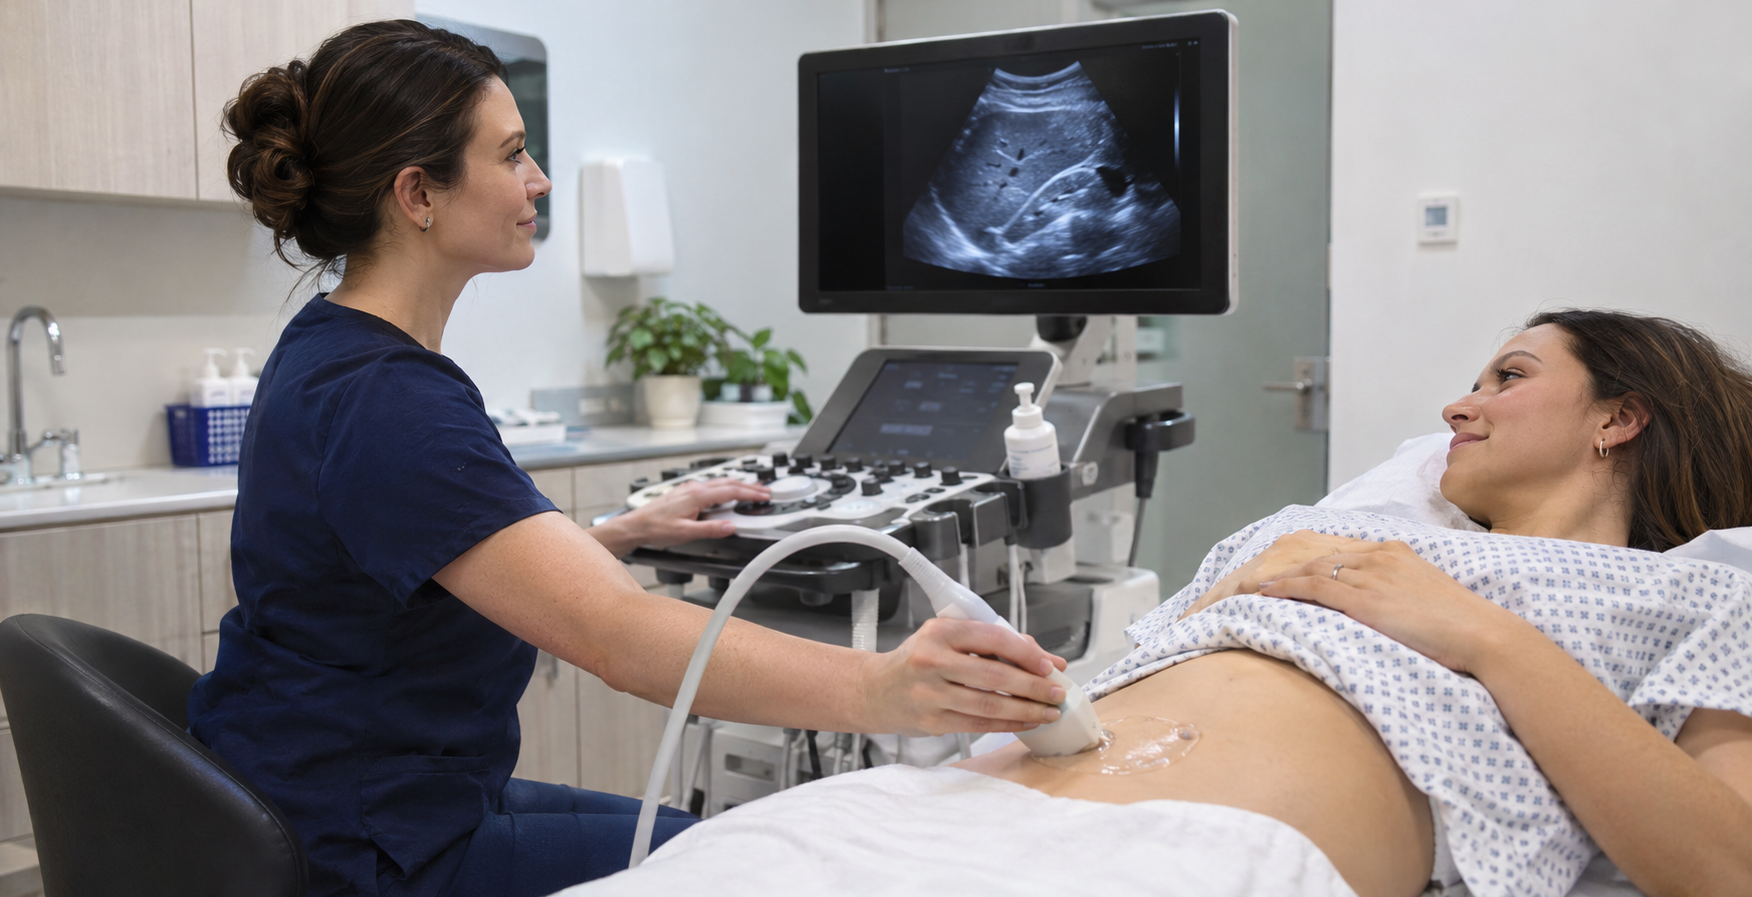
\includegraphics[width=\textwidth,keepaspectratio]{modalities/infographics/ultrasound_realistic.png}
\end{center}
\begin{center}\footnotesize Coupling gel removes air between the probe and skin so sound can enter the body; the returning echoes form a real-time image. Gas and bone can limit the acoustic window. AI-generated illustration; the ultrasound panel is not a clinical study.\end{center}

\section{Overview}
Diagnostic ultrasound (ultrasonography) uses high-frequency sound waves to visualize anatomical structures, blood flow, tissue abnormalities, and physiological movements in real time. Unlike conventional X-rays, ultrasound does not use ionizing radiation.

This catalogue covers diseases and conditions for which ultrasound has established clinical diagnostic utility. It includes conventional B-mode ultrasound, Doppler ultrasound, echocardiography, transvaginal ultrasound, and musculoskeletal ultrasound, while excluding purely therapeutic applications and procedural guidance.

The 263 entries form a preliminary catalogue of diseases, conditions, and observable abnormalities. They are not all independently diagnosable using ultrasound; some require alternative imaging, histopathology, or laboratory confirmation. Individual guideline validation is necessary before using this catalogue as diagnostic ground truth.

\section{Where ultrasound is used}
The following numbered entries present common diagnostic applications by anatomical system. Ultrasound may detect or characterize an abnormality without establishing its cause. A negative study does not exclude disease when sensitivity is limited. Findings should be interpreted with symptoms, examination, laboratory results, and other imaging.

\subsection{Liver}
\begin{enumerate}[leftmargin=*,itemsep=0.45em,topsep=0.4em]
\item \textbf{Budd--Chiari syndrome.} Useful imaging findings include: Hepatic venous obstruction.
\item \textbf{Congestive hepatopathy.} Useful imaging findings include: Dilated hepatic veins and inferior vena cava.
\item \textbf{Hepatic hemangioma.} Useful imaging findings include: Well-defined hyperechoic lesion.
\item \textbf{Hepatic metastases.} Useful imaging findings include: Multiple lesions may be detected, sometimes with a target appearance. Appearance alone cannot establish metastatic origin.
\item \textbf{Hepatic steatosis.} Useful imaging findings include: Increased hepatic echogenicity.
\item \textbf{Hepatocellular carcinoma.} Useful imaging findings include: Surveillance may detect a liver observation in an at-risk patient. A solid lesion is nonspecific and requires diagnostic characterization.
\item \textbf{Hepatomegaly.} Useful imaging findings include: Increased liver dimensions.
\item \textbf{Hydatid cyst.} Useful imaging findings include: Daughter cysts, detached membranes.
\item \textbf{Liver abscess.} Useful imaging findings include: Complex hypoechoic lesion with internal debris.
\item \textbf{Liver cirrhosis.} Useful imaging findings include: Nodular surface, coarse echotexture.
\item \textbf{Polycystic liver disease.} Useful imaging findings include: Multiple hepatic cysts.
\item \textbf{Portal hypertension.} Useful imaging findings include: Portosystemic collaterals, abnormal portal flow.
\item \textbf{Portal vein thrombosis.} Useful imaging findings include: Intraluminal thrombus, absent or reduced flow.
\item \textbf{Simple hepatic cyst.} Useful imaging findings include: Anechoic lesion with posterior acoustic enhancement.
\end{enumerate}

\subsection{Gallbladder and biliary system}
\begin{enumerate}[leftmargin=*,itemsep=0.45em,topsep=0.4em]
\item \textbf{Acalculous cholecystitis.} Useful imaging findings include: Inflammatory changes without gallstones.
\item \textbf{Acute cholecystitis.} Useful imaging findings include: Wall thickening, pericholecystic fluid, sonographic Murphy sign.
\item \textbf{Adenomyomatosis.} Useful imaging findings include: Comet-tail artifacts, intramural cystic spaces.
\item \textbf{Biliary obstruction.} Useful imaging findings include: Dilated bile ducts.
\item \textbf{Choledochal cyst.} Useful imaging findings include: Cystic bile duct dilatation.
\item \textbf{Choledocholithiasis.} Useful imaging findings include: Echogenic bile duct calculi.
\item \textbf{Cholelithiasis.} Useful imaging findings include: Echogenic calculi with posterior acoustic shadowing.
\item \textbf{Chronic cholecystitis.} Useful imaging findings include: Contracted gallbladder, wall thickening.
\item \textbf{Gallbladder carcinoma.} Useful imaging findings include: Irregular mass or asymmetric wall thickening.
\item \textbf{Gallbladder hydrops.} Useful imaging findings include: Markedly distended gallbladder.
\item \textbf{Gallbladder polyps.} Useful imaging findings include: Nonmobile mural projections.
\item \textbf{Gallbladder sludge.} Useful imaging findings include: Dependent low-level echoes.
\end{enumerate}

\subsection{Pancreas}
\begin{enumerate}[leftmargin=*,itemsep=0.45em,topsep=0.4em]
\item \textbf{Acute pancreatitis.} Useful imaging findings include: Enlarged hypoechoic pancreas.
\item \textbf{Chronic pancreatitis.} Useful imaging findings include: Heterogeneous echotexture, calcifications.
\item \textbf{Pancreatic calcification.} Useful imaging findings include: Echogenic foci with acoustic shadowing.
\item \textbf{Pancreatic carcinoma.} Useful imaging findings include: Irregular hypoechoic mass.
\item \textbf{Pancreatic cyst.} Useful imaging findings include: Anechoic or complex cystic lesion.
\item \textbf{Pancreatic duct dilatation.} Useful imaging findings include: Enlarged pancreatic duct.
\item \textbf{Pancreatic pseudocyst.} Useful imaging findings include: Encapsulated fluid collection.
\end{enumerate}

Transabdominal ultrasound has limitations in pancreatic imaging because of overlying bowel gas. CT, MRI, and endoscopic ultrasound are frequently preferred.

\subsection{Kidneys}
\begin{enumerate}[leftmargin=*,itemsep=0.45em,topsep=0.4em]
\item \textbf{Acute pyelonephritis.} Useful imaging findings include: Ultrasound may be normal or show nonspecific focal swelling or altered echogenicity. It is mainly used to assess obstruction or complications.
\item \textbf{Chronic kidney disease.} Useful imaging findings include: Increased cortical echogenicity, cortical thinning.
\item \textbf{Complex renal cyst.} Useful imaging findings include: Internal septations or solid components.
\item \textbf{Duplex collecting system.} Useful imaging findings include: Duplicated renal collecting structures.
\item \textbf{Ectopic kidney.} Useful imaging findings include: Abnormal renal location.
\item \textbf{Horseshoe kidney.} Useful imaging findings include: Fusion of renal poles.
\item \textbf{Hydronephrosis.} Useful imaging findings include: Dilated renal collecting system.
\item \textbf{Medullary nephrocalcinosis.} Useful imaging findings include: Echogenic renal pyramids.
\item \textbf{Multicystic dysplastic kidney.} Useful imaging findings include: Multiple noncommunicating cysts.
\item \textbf{Nephrolithiasis.} Useful imaging findings include: Echogenic calculus with acoustic shadowing.
\item \textbf{Polycystic kidney disease.} Useful imaging findings include: Multiple bilateral renal cysts.
\item \textbf{Renal abscess.} Useful imaging findings include: Complex fluid collection.
\item \textbf{Renal angiomyolipoma.} Useful imaging findings include: Typically hyperechoic renal mass.
\item \textbf{Renal artery stenosis.} Useful imaging findings include: Doppler may show increased velocity. Technical limitations can affect the study, and stenosis alone does not establish renovascular hypertension.
\item \textbf{Renal atrophy.} Useful imaging findings include: Reduced renal dimensions.
\item \textbf{Renal cell carcinoma.} Useful imaging findings include: Solid renal mass.
\item \textbf{Renal vein thrombosis.} Useful imaging findings include: Abnormal or absent venous flow may support thrombosis. Further imaging may be needed when the examination is limited or equivocal.
\item \textbf{Simple renal cyst.} Useful imaging findings include: Anechoic, thin-walled lesion.
\end{enumerate}

\subsection{Urinary bladder and prostate}
\begin{enumerate}[leftmargin=*,itemsep=0.45em,topsep=0.4em]
\item \textbf{Benign prostatic hyperplasia.} Useful imaging findings include: Increased prostate volume.
\item \textbf{Bladder diverticulum.} Useful imaging findings include: Outpouching of the bladder wall.
\item \textbf{Bladder outlet obstruction.} Useful imaging findings include: Increased postvoid residual, trabeculation.
\item \textbf{Bladder stones.} Useful imaging findings include: Mobile echogenic structures with shadowing.
\item \textbf{Bladder tumor.} Useful imaging findings include: Mural soft-tissue mass.
\item \textbf{Prostatic abscess.} Useful imaging findings include: Complex hypoechoic collection.
\item \textbf{Prostatic cyst.} Useful imaging findings include: Anechoic intraprostatic lesion.
\item \textbf{Ureterocele.} Useful imaging findings include: Cystic structure near the ureteric orifice.
\item \textbf{Urinary retention.} Useful imaging findings include: Distended urinary bladder.
\end{enumerate}

\subsection{Spleen}
\begin{enumerate}[leftmargin=*,itemsep=0.45em,topsep=0.4em]
\item \textbf{Splenic abscess.} Useful imaging findings include: Complex hypoechoic collection.
\item \textbf{Splenic cyst.} Useful imaging findings include: Anechoic lesion.
\item \textbf{Splenic hemangioma.} Useful imaging findings include: Focal lesion with variable echogenicity.
\item \textbf{Splenic hematoma.} Useful imaging findings include: Subcapsular or intraparenchymal collection.
\item \textbf{Splenic infarction.} Useful imaging findings include: Peripheral wedge-shaped hypoechoic region.
\item \textbf{Splenic rupture.} Useful imaging findings include: Parenchymal disruption, perisplenic fluid.
\item \textbf{Splenomegaly.} Useful imaging findings include: Increased splenic dimensions.
\end{enumerate}

\subsection{Gastrointestinal system}
\begin{enumerate}[leftmargin=*,itemsep=0.45em,topsep=0.4em]
\item \textbf{Acute appendicitis.} Useful imaging findings include: A dilated, noncompressible appendix supports the diagnosis when visualized. Nonvisualization does not exclude appendicitis.
\item \textbf{Crohn disease.} Useful imaging findings include: Bowel wall thickening, increased vascularity.
\item \textbf{Diverticulitis.} Useful imaging findings include: Inflamed diverticulum, surrounding echogenic fat.
\item \textbf{Hypertrophic pyloric stenosis.} Useful imaging findings include: Thickened and elongated pyloric muscle.
\item \textbf{Incisional hernia.} Useful imaging findings include: Herniation through a surgical defect.
\item \textbf{Inguinal hernia.} Useful imaging findings include: Protrusion of abdominal contents.
\item \textbf{Intussusception.} Useful imaging findings include: Target sign, pseudokidney sign.
\item \textbf{Mesenteric lymphadenitis.} Useful imaging findings include: Enlarged mesenteric lymph nodes.
\item \textbf{Midgut volvulus.} Useful imaging findings include: Whirlpool sign.
\item \textbf{Necrotizing enterocolitis.} Useful imaging findings include: Ultrasound may show bowel-wall pneumatosis, thinning, absent perfusion, or complex fluid. It supplements radiographs and clinical assessment.
\item \textbf{Small bowel obstruction.} Useful imaging findings include: Dilated fluid-filled bowel loops.
\item \textbf{Ulcerative colitis.} Useful imaging findings include: Colonic wall thickening.
\item \textbf{Umbilical hernia.} Useful imaging findings include: Herniation through an umbilical defect.
\end{enumerate}

\subsection{Female reproductive system}
\begin{enumerate}[leftmargin=*,itemsep=0.45em,topsep=0.4em]
\item \textbf{Adenomyosis.} Useful imaging findings include: Heterogeneous myometrium, myometrial cysts.
\item \textbf{Bicornuate uterus.} Useful imaging findings include: Two uterine horns and external fundal cleft.
\item \textbf{Cesarean scar defect.} Useful imaging findings include: Hypoechoic indentation at the uterine scar.
\item \textbf{Endometrial carcinoma.} Useful imaging findings include: Irregular endometrial thickening or mass.
\item \textbf{Endometrial hyperplasia.} Useful imaging findings include: Endometrial thickening.
\item \textbf{Endometrial polyp.} Useful imaging findings include: Focal endometrial lesion, feeding vessel.
\item \textbf{Hemorrhagic ovarian cyst.} Useful imaging findings include: Reticular internal echoes.
\item \textbf{Hydrosalpinx.} Useful imaging findings include: Elongated fluid-filled tubular structure.
\item \textbf{Ovarian carcinoma.} Useful imaging findings include: A complex mass with solid tissue or papillary projections is suspicious but cannot establish histology.
\item \textbf{Ovarian dermoid cyst.} Useful imaging findings include: Echogenic components, acoustic shadowing.
\item \textbf{Ovarian endometrioma.} Useful imaging findings include: Ground-glass internal echoes.
\item \textbf{Ovarian torsion.} Useful imaging findings include: An enlarged ovary or twisted pedicle supports torsion. Preserved Doppler flow does not exclude it.
\item \textbf{Pelvic endometriosis.} Useful imaging findings include: Expert ultrasound may detect some deep endometriotic lesions. A normal scan does not exclude superficial disease.
\item \textbf{Pelvic organ prolapse.} Useful imaging findings include: Dynamic descent of pelvic structures.
\item \textbf{Polycystic ovarian morphology.} Useful imaging findings include: Increased follicle number or ovarian volume may meet imaging criteria. This morphology alone does not diagnose polycystic ovary syndrome.
\item \textbf{Pyosalpinx.} Useful imaging findings include: Dilated tube with internal debris.
\item \textbf{Retained products of conception.} Useful imaging findings include: Intrauterine echogenic tissue, variable vascularity.
\item \textbf{Septate uterus.} Useful imaging findings include: Internal uterine septum.
\item \textbf{Simple ovarian cyst.} Useful imaging findings include: Thin-walled anechoic lesion.
\item \textbf{Tubo-ovarian abscess.} Useful imaging findings include: Complex inflammatory adnexal mass.
\item \textbf{Unicornuate uterus.} Useful imaging findings include: Asymmetric single uterine horn.
\item \textbf{Uterine fibroids.} Useful imaging findings include: Well-defined solid myometrial masses.
\end{enumerate}

\subsection{Obstetric and fetal conditions}
\begin{enumerate}[leftmargin=*,itemsep=0.45em,topsep=0.4em]
\item \textbf{Anembryonic pregnancy.} Useful imaging findings include: Empty gestational sac meeting diagnostic criteria.
\item \textbf{Anencephaly.} Useful imaging findings include: Absence of major cranial structures.
\item \textbf{Cervical insufficiency.} Useful imaging findings include: Shortened cervix, cervical funneling.
\item \textbf{Congenital diaphragmatic hernia.} Useful imaging findings include: Abdominal organs within the fetal thorax.
\item \textbf{Early pregnancy loss.} Useful imaging findings include: Absent embryonic cardiac activity meeting diagnostic criteria.
\item \textbf{Ectopic pregnancy.} Useful imaging findings include: Extrauterine gestational sac or adnexal mass.
\item \textbf{Fetal congenital heart defects.} Useful imaging findings include: Targeted fetal echocardiography can identify many structural defects. Routine screening does not detect every defect.
\item \textbf{Fetal growth restriction.} Useful imaging findings include: Estimated fetal weight or abdominal circumference is interpreted by gestational-age percentiles and clinical context. A single small measurement alone may not establish pathologic growth restriction.
\item \textbf{Fetal hydrocephalus.} Useful imaging findings include: Ventricular dilatation.
\item \textbf{Fetal hydronephrosis.} Useful imaging findings include: Dilated renal collecting system.
\item \textbf{Fetal hydrops.} Useful imaging findings include: Abnormal fluid in multiple fetal compartments.
\item \textbf{Fetal macrosomia.} Useful imaging findings include: Increased estimated fetal weight.
\item \textbf{Fetal renal agenesis.} Useful imaging findings include: Absent renal structures.
\item \textbf{Fetal skeletal dysplasia.} Useful imaging findings include: Disproportionate measurements or abnormal bone morphology may raise suspicion. Some dysplasias are not detectable on routine ultrasound.
\item \textbf{Gastroschisis.} Useful imaging findings include: Externalized bowel without a covering membrane.
\item \textbf{Hydatidiform mole.} Useful imaging findings include: Multicystic intrauterine tissue.
\item \textbf{Oligohydramnios.} Useful imaging findings include: Reduced amniotic fluid volume.
\item \textbf{Omphalocele.} Useful imaging findings include: Membrane-covered abdominal wall defect.
\item \textbf{Placenta accreta spectrum.} Useful imaging findings include: Placental lacunae, abnormal vascularity.
\item \textbf{Placenta previa.} Useful imaging findings include: Placenta covering the internal cervical os.
\item \textbf{Placental abruption.} Useful imaging findings include: A retroplacental hematoma may be visible. A normal ultrasound does not exclude abruption.
\item \textbf{Polyhydramnios.} Useful imaging findings include: Increased amniotic fluid volume.
\item \textbf{Spina bifida.} Useful imaging findings include: Spinal defect, associated cranial signs.
\item \textbf{Twin-to-twin transfusion syndrome.} Useful imaging findings include: Discordant amniotic fluid volumes.
\item \textbf{Vasa previa.} Useful imaging findings include: Fetal vessels crossing the internal cervical os.
\end{enumerate}

\subsection{Breast}
\begin{enumerate}[leftmargin=*,itemsep=0.45em,topsep=0.4em]
\item \textbf{Breast abscess.} Useful imaging findings include: Complex fluid collection.
\item \textbf{Breast carcinoma.} Useful imaging findings include: An irregular nonparallel mass may be suspicious. Ultrasound appearance cannot establish histology, which requires biopsy.
\item \textbf{Breast hematoma.} Useful imaging findings include: Complex fluid collection.
\item \textbf{Complicated breast cyst.} Useful imaging findings include: Internal low-level echoes.
\item \textbf{Duct ectasia.} Useful imaging findings include: Dilated mammary ducts.
\item \textbf{Fat necrosis.} Useful imaging findings include: Variable cystic or solid appearance.
\item \textbf{Fibroadenoma.} Useful imaging findings include: Oval, circumscribed hypoechoic mass.
\item \textbf{Galactocele.} Useful imaging findings include: Variable echogenicity, sometimes fat-fluid level.
\item \textbf{Intraductal papilloma.} Useful imaging findings include: Solid intraductal mass.
\item \textbf{Mastitis.} Useful imaging findings include: Increased vascularity and tissue edema.
\item \textbf{Phyllodes tumor.} Useful imaging findings include: A large heterogeneous mass may raise suspicion, but imaging cannot reliably distinguish phyllodes tumor from fibroadenoma or establish its grade.
\item \textbf{Postoperative seroma.} Useful imaging findings include: Fluid collection.
\item \textbf{Silicone implant rupture.} Useful imaging findings include: A stepladder sign can indicate intracapsular rupture and a snowstorm appearance can indicate extracapsular silicone. Equivocal examinations may require MRI.
\item \textbf{Simple breast cyst.} Useful imaging findings include: Anechoic lesion with posterior enhancement.
\end{enumerate}

\subsection{Thyroid and parathyroid glands}
\begin{enumerate}[leftmargin=*,itemsep=0.45em,topsep=0.4em]
\item \textbf{Follicular thyroid neoplasm.} Useful imaging findings include: Ultrasound can characterize a solid nodule but cannot distinguish follicular adenoma from carcinoma. Histology assessing capsular or vascular invasion is required.
\item \textbf{Graves disease.} Useful imaging findings include: Diffuse hypervascularity.
\item \textbf{Hashimoto thyroiditis.} Useful imaging findings include: Heterogeneous hypoechoic gland.
\item \textbf{Multinodular goiter.} Useful imaging findings include: Multiple thyroid nodules.
\item \textbf{Papillary thyroid carcinoma.} Useful imaging findings include: Suspicious hypoechoic nodule, punctate echogenic foci.
\item \textbf{Parathyroid adenoma.} Useful imaging findings include: A hypoechoic lesion can help localize a suspected abnormal gland. Ultrasound does not establish biochemical hyperparathyroidism.
\item \textbf{Subacute thyroiditis.} Useful imaging findings include: Patchy hypoechoic regions.
\item \textbf{Thyroid abscess.} Useful imaging findings include: Complex fluid collection.
\item \textbf{Thyroid cyst.} Useful imaging findings include: Anechoic or complex cystic lesion.
\item \textbf{Thyroid nodule.} Useful imaging findings include: Focal solid, cystic, or mixed lesion.
\end{enumerate}

\subsection{Cardiovascular system: echocardiography}
\begin{enumerate}[leftmargin=*,itemsep=0.45em,topsep=0.4em]
\item \textbf{Aortic regurgitation.} Useful imaging findings include: Retrograde diastolic blood flow.
\item \textbf{Aortic stenosis.} Useful imaging findings include: Restricted valve opening, increased flow velocity.
\item \textbf{Atrial myxoma.} Useful imaging findings include: Mobile intracardiac mass.
\item \textbf{Atrial septal defect.} Useful imaging findings include: Interatrial communication.
\item \textbf{Cardiac tamponade.} Useful imaging findings include: Chamber collapse, abnormal respiratory flow variation.
\item \textbf{Constrictive pericarditis.} Useful imaging findings include: Abnormal septal motion, ventricular interdependence.
\item \textbf{Dilated cardiomyopathy.} Useful imaging findings include: Dilated ventricles, reduced contractility.
\item \textbf{Heart failure with preserved ejection fraction.} Useful imaging findings include: Echocardiographic structure and diastolic indices support assessment. Filling pressure estimates are imperfect and must be interpreted with clinical findings.
\item \textbf{Heart failure with reduced ejection fraction.} Useful imaging findings include: Reduced left ventricular ejection fraction.
\item \textbf{Hypertrophic cardiomyopathy.} Useful imaging findings include: Abnormal myocardial thickening.
\item \textbf{Infective endocarditis.} Useful imaging findings include: Echocardiography may show vegetations or complications. A negative transthoracic study does not exclude endocarditis when suspicion remains high. Transesophageal echocardiography may be needed.
\item \textbf{Left ventricular thrombus.} Useful imaging findings include: Intracavitary mass.
\item \textbf{Mitral regurgitation.} Useful imaging findings include: Retrograde systolic blood flow.
\item \textbf{Mitral stenosis.} Useful imaging findings include: Restricted mitral valve opening.
\item \textbf{Mitral valve prolapse.} Useful imaging findings include: Systolic leaflet displacement.
\item \textbf{Patent ductus arteriosus.} Useful imaging findings include: Persistent abnormal vascular connection.
\item \textbf{Pericardial effusion.} Useful imaging findings include: Fluid surrounding the heart.
\item \textbf{Pulmonary hypertension.} Useful imaging findings include: Echocardiography estimates the probability and pressure. Right-heart catheterization confirms the hemodynamic diagnosis.
\item \textbf{Pulmonary valve stenosis.} Useful imaging findings include: Increased transvalvular flow velocity.
\item \textbf{Regional myocardial dysfunction.} Useful imaging findings include: Regional wall-motion abnormalities.
\item \textbf{Restrictive cardiomyopathy.} Useful imaging findings include: Abnormal ventricular filling.
\item \textbf{Tetralogy of Fallot.} Useful imaging findings include: Characteristic congenital cardiac abnormalities.
\item \textbf{Tricuspid regurgitation.} Useful imaging findings include: Retrograde flow across the tricuspid valve.
\item \textbf{Ventricular aneurysm.} Useful imaging findings include: Abnormal ventricular outpouching.
\item \textbf{Ventricular septal defect.} Useful imaging findings include: Interventricular communication.
\end{enumerate}

\subsection{Vascular system: Doppler ultrasound}
\begin{enumerate}[leftmargin=*,itemsep=0.45em,topsep=0.4em]
\item \textbf{Abdominal aortic aneurysm.} Useful imaging findings include: Increased aortic diameter.
\item \textbf{Acute arterial occlusion.} Useful imaging findings include: Absent arterial flow.
\item \textbf{Arterial pseudoaneurysm.} Useful imaging findings include: To-and-fro flow at the neck.
\item \textbf{Arteriovenous fistula.} Useful imaging findings include: High-velocity turbulent flow.
\item \textbf{Arteriovenous malformation.} Useful imaging findings include: Abnormal vascular channels.
\item \textbf{Carotid artery stenosis.} Useful imaging findings include: Doppler velocity and plaque support stenosis grading. Confirmatory imaging may be needed for intervention planning.
\item \textbf{Chronic venous insufficiency.} Useful imaging findings include: Abnormal venous reflux.
\item \textbf{Deep vein thrombosis.} Useful imaging findings include: Noncompressible vein.
\item \textbf{Peripheral arterial aneurysm.} Useful imaging findings include: Focal arterial dilatation.
\item \textbf{Peripheral arterial disease.} Useful imaging findings include: Abnormal waveforms suggest disease. Duplex assessment and ankle-brachial index help determine its location and hemodynamic significance.
\item \textbf{Subclavian steal syndrome.} Useful imaging findings include: Reversed vertebral arterial flow.
\item \textbf{Superficial venous thrombosis.} Useful imaging findings include: Intraluminal venous thrombus.
\item \textbf{Varicose veins.} Useful imaging findings include: Dilated tortuous superficial veins.
\end{enumerate}

\subsection{Musculoskeletal system}
\begin{enumerate}[leftmargin=*,itemsep=0.45em,topsep=0.4em]
\item \textbf{Achilles tendon rupture.} Useful imaging findings include: Disrupted tendon fibers.
\item \textbf{Baker cyst.} Useful imaging findings include: Popliteal fluid collection.
\item \textbf{Bursitis.} Useful imaging findings include: Fluid-filled distended bursa.
\item \textbf{Calcific tendinitis.} Useful imaging findings include: Echogenic intratendinous deposits.
\item \textbf{Carpal tunnel syndrome.} Useful imaging findings include: Enlarged median nerve.
\item \textbf{CPPD disease.} Useful imaging findings include: Cartilage deposits may be seen. The appearance is operator-dependent and does not replace crystal analysis when confirmation is needed.
\item \textbf{Developmental dysplasia of the hip.} Useful imaging findings include: Abnormal femoral head coverage.
\item \textbf{Enthesitis.} Useful imaging findings include: Tendon insertion abnormalities.
\item \textbf{Ganglion cyst.} Useful imaging findings include: Cystic periarticular lesion.
\item \textbf{Gout.} Useful imaging findings include: The double-contour sign or tophi can support gout. Absence of these findings does not exclude early disease, and other crystal disease can overlap.
\item \textbf{Joint effusion.} Useful imaging findings include: Intra-articular fluid.
\item \textbf{Morton neuroma.} Useful imaging findings include: Hypoechoic interdigital mass.
\item \textbf{Muscle hematoma.} Useful imaging findings include: Intramuscular collection.
\item \textbf{Muscle tear.} Useful imaging findings include: Disrupted muscle architecture.
\item \textbf{Plantar fasciitis.} Useful imaging findings include: Thickened plantar fascia.
\item \textbf{Rheumatoid arthritis.} Useful imaging findings include: Ultrasound can show synovitis, Doppler activity, and erosions. These findings are not specific and do not replace clinical classification.
\item \textbf{Rotator cuff tear.} Useful imaging findings include: Tendon discontinuity.
\item \textbf{Synovitis.} Useful imaging findings include: Synovial thickening and hypervascularity.
\item \textbf{Tendinopathy.} Useful imaging findings include: Tendon thickening and altered echogenicity.
\item \textbf{Tenosynovitis.} Useful imaging findings include: Tendon sheath fluid and inflammation.
\item \textbf{Trigger finger.} Useful imaging findings include: Thickening of the A1 pulley.
\item \textbf{Ulnar nerve entrapment.} Useful imaging findings include: Enlarged or dynamically displaced ulnar nerve.
\end{enumerate}

\subsection{Male reproductive system}
\begin{enumerate}[leftmargin=*,itemsep=0.45em,topsep=0.4em]
\item \textbf{Epididymitis.} Useful imaging findings include: Enlarged hypervascular epididymis.
\item \textbf{Hematocele.} Useful imaging findings include: Complex fluid surrounding the testicle.
\item \textbf{Hydrocele.} Useful imaging findings include: Fluid surrounding the testicle.
\item \textbf{Orchitis.} Useful imaging findings include: Increased testicular vascularity.
\item \textbf{Spermatocele.} Useful imaging findings include: Cystic epididymal lesion.
\item \textbf{Testicular abscess.} Useful imaging findings include: Complex intratesticular collection.
\item \textbf{Testicular carcinoma.} Useful imaging findings include: Solid intratesticular mass.
\item \textbf{Testicular microlithiasis.} Useful imaging findings include: Multiple punctate echogenic foci.
\item \textbf{Testicular rupture.} Useful imaging findings include: Disruption of the tunica albuginea.
\item \textbf{Testicular torsion.} Useful imaging findings include: A twisted spermatic cord or reduced flow supports torsion. Preserved flow can occur and does not exclude torsion.
\item \textbf{Undescended testicle.} Useful imaging findings include: Testicle outside its normal scrotal location.
\item \textbf{Varicocele.} Useful imaging findings include: Dilated veins with reflux.
\end{enumerate}

\subsection{Ophthalmology}
\begin{enumerate}[leftmargin=*,itemsep=0.45em,topsep=0.4em]
\item \textbf{Choroidal detachment.} Useful imaging findings include: Dome-shaped elevated choroidal membranes.
\item \textbf{Choroidal melanoma.} Useful imaging findings include: Solid intraocular mass.
\item \textbf{Dislocated crystalline lens.} Useful imaging findings include: Abnormal lens position.
\item \textbf{Intraocular foreign body.} Useful imaging findings include: Echogenic foreign object.
\item \textbf{Optic disc drusen.} Useful imaging findings include: Highly reflective calcified deposits.
\item \textbf{Posterior scleritis.} Useful imaging findings include: A T-sign may be visible on B-scan ultrasound. Ophthalmic examination and other imaging may be needed.
\item \textbf{Posterior vitreous detachment.} Useful imaging findings include: Mobile detached vitreous membrane.
\item \textbf{Retinal detachment.} Useful imaging findings include: Elevated retinal membrane.
\item \textbf{Retinoblastoma.} Useful imaging findings include: Intraocular mass with possible calcifications.
\item \textbf{Vitreous hemorrhage.} Useful imaging findings include: Mobile internal vitreous echoes.
\end{enumerate}

\subsection{Pulmonary and thoracic ultrasound}
\begin{enumerate}[leftmargin=*,itemsep=0.45em,topsep=0.4em]
\item \textbf{Atelectasis.} Useful imaging findings include: Tissue-like lung appearance.
\item \textbf{Diaphragmatic paralysis.} Useful imaging findings include: Absent or paradoxical diaphragmatic movement.
\item \textbf{Empyema.} Useful imaging findings include: Complex or septated pleural fluid.
\item \textbf{Peripheral pneumonia.} Useful imaging findings include: Subpleural consolidation, air bronchograms.
\item \textbf{Peripheral pulmonary infarction.} Useful imaging findings include: A pleural-based wedge-shaped lesion may be visible but is nonspecific. Ultrasound cannot exclude pulmonary embolism or confirm infarction alone.
\item \textbf{Pleural effusion.} Useful imaging findings include: Fluid within the pleural space.
\item \textbf{Pneumothorax.} Useful imaging findings include: Absent lung sliding, lung point when visible.
\item \textbf{Pulmonary edema.} Useful imaging findings include: Multiple bilateral B-lines.
\end{enumerate}

\subsection{Superficial soft tissues and lymph nodes}
\begin{enumerate}[leftmargin=*,itemsep=0.45em,topsep=0.4em]
\item \textbf{Cellulitis.} Useful imaging findings include: Cobblestone appearance.
\item \textbf{Epidermoid cyst.} Useful imaging findings include: Circumscribed lesion with internal echoes.
\item \textbf{Lipoma.} Useful imaging findings include: Usually well-defined soft-tissue mass.
\item \textbf{Lymphedema.} Useful imaging findings include: Subcutaneous edema.
\item \textbf{Lymphoma.} Useful imaging findings include: Enlarged hypoechoic lymph nodes.
\item \textbf{Metastatic lymphadenopathy.} Useful imaging findings include: Abnormal nodal morphology.
\item \textbf{Pilomatricoma.} Useful imaging findings include: Superficial mass with calcifications.
\item \textbf{Reactive lymphadenopathy.} Useful imaging findings include: Enlarged nodes with preserved fatty hilum.
\item \textbf{Soft-tissue abscess.} Useful imaging findings include: Complex fluid collection.
\item \textbf{Soft-tissue foreign body.} Useful imaging findings include: Echogenic object with surrounding inflammation.
\end{enumerate}

\subsection{Neonatal cranial ultrasound}
\begin{enumerate}[leftmargin=*,itemsep=0.45em,topsep=0.4em]
\item \textbf{Agenesis of the corpus callosum.} Useful imaging findings include: Abnormal midline anatomy.
\item \textbf{Dandy--Walker malformation.} Useful imaging findings include: Abnormal posterior fossa structures.
\item \textbf{Germinal matrix hemorrhage.} Useful imaging findings include: Echogenic focus at the caudothalamic groove.
\item \textbf{Hydrocephalus.} Useful imaging findings include: Ventricular enlargement.
\item \textbf{Intraventricular hemorrhage.} Useful imaging findings include: Echogenic intraventricular blood.
\item \textbf{Periventricular leukomalacia.} Useful imaging findings include: Periventricular echogenicity or cystic changes.
\item \textbf{Porencephalic cyst.} Useful imaging findings include: Intracerebral cystic cavity.
\end{enumerate}

\subsection{Emergency abdominal ultrasound}
\begin{enumerate}[leftmargin=*,itemsep=0.45em,topsep=0.4em]
\item \textbf{Abdominal abscess.} Useful imaging findings include: Complex fluid collection.
\item \textbf{Abdominal hematoma.} Useful imaging findings include: Collection with variable echogenicity.
\item \textbf{Ascites.} Useful imaging findings include: Free intraperitoneal fluid.
\item \textbf{Hemoperitoneum.} Useful imaging findings include: Free intraperitoneal fluid in a trauma setting.
\item \textbf{Retroperitoneal mass.} Useful imaging findings include: Abnormal retroperitoneal lesion.
\end{enumerate}

\subsection{Summary}
\begin{center}
\begin{tabular}{@{}lr@{}}
\toprule
\textbf{Anatomical system} & \textbf{Conditions} \\
\midrule
Breast & 14 \\
Echocardiography & 25 \\
Emergency abdominal ultrasound & 5 \\
Female reproductive system & 22 \\
Gallbladder and biliary system & 12 \\
Gastrointestinal system & 13 \\
Kidneys & 18 \\
Liver & 14 \\
Male reproductive system & 12 \\
Musculoskeletal system & 22 \\
Neonatal cranial ultrasound & 7 \\
Obstetrics and fetal medicine & 25 \\
Ophthalmology & 10 \\
Pancreas & 7 \\
Pulmonary and thoracic system & 8 \\
Spleen & 7 \\
Superficial soft tissues & 10 \\
Thyroid and parathyroid glands & 10 \\
\textbf{Total} & \textbf{263} \\
Urinary bladder and prostate & 9 \\
\midrule
Vascular system & 13 \\
\bottomrule
\end{tabular}
\end{center}

\subsection{Authoritative sources for published ultrasound images}
\begin{longtable}{@{}p{0.40\textwidth}p{0.54\textwidth}@{}}
\toprule
\textbf{Source} & \textbf{Primary utility} \\
\midrule
\endfirsthead
\toprule
\textbf{Source} & \textbf{Primary utility} \\
\midrule
\endhead
ACR Appropriateness Criteria & Clinical indications for diagnostic imaging \\
American Institute of Ultrasound in Medicine & Ultrasound practice parameters \\
American Society of Echocardiography & Cardiac ultrasound \\
International Society of Ultrasound in Obstetrics and Gynecology & Obstetric and gynecological ultrasound \\
PubMed Central & Published clinical sonograms \\
Radiopaedia & Annotated diagnostic imaging cases \\
The Radiology Assistant & Radiological interpretation \\
UltrasoundCases.info & Clinical ultrasound pathology atlas \\
\bottomrule
\end{longtable}

\subsection{Acquisition techniques for dataset development}
For medical imaging dataset development, ultrasound images should additionally be classified by acquisition technique:
\begin{itemize}
    \item B-mode ultrasound
    \item M-mode ultrasound
    \item Color Doppler
    \item Power Doppler
    \item Spectral Doppler
    \item Contrast-enhanced ultrasound
    \item Ultrasound elastography
    \item 3D ultrasound
    \item 4D ultrasound
\end{itemize}

Ultrasound is used in the medical assessment of every condition listed here, but its role varies. Some entries name a sonographic finding rather than a disease that can be diagnosed from the image alone. A normal or technically limited examination may not exclude disease. Suspicious masses, suspected vascular disease, and clinically important negative examinations may require additional imaging, laboratory tests, pathology, or specialist assessment.

\subsection{Selected clinical guidance}
\begin{itemize}
    \item Society of Maternal-Fetal Medicine. \href{https://publications.smfm.org/publications/289-society-for-maternal-fetal-medicine-consult-series-52/}{Diagnosis and management of fetal growth restriction}.
    \item American College of Obstetricians and Gynecologists. \href{https://www.acog.org/clinical/clinical-guidance/committee-opinion/articles/2019/08/adnexal-torsion-in-adolescents}{Adnexal torsion in adolescents}.
    \item European Society of Cardiology. \href{https://academic.oup.com/eurheartj/article/44/39/3948/7243107}{Guidelines for the management of endocarditis}.
    \item American College of Radiology. \href{https://acsearch.acr.org/docs/3100728/Narrative/}{Appropriateness Criteria for breast implant evaluation}.
    \item American Society of Echocardiography. \href{https://www.asecho.org/wp-content/uploads/2025/07/Left-Ventricular-Diastolic-Function.pdf}{Recommendations for evaluation of left ventricular diastolic function and HFpEF}.
\end{itemize}

\chapter{Doppler Ultrasound}
\label{ch:ch15_doppler}

% Chapter-opening illustrated modality infographic.
\begin{center}
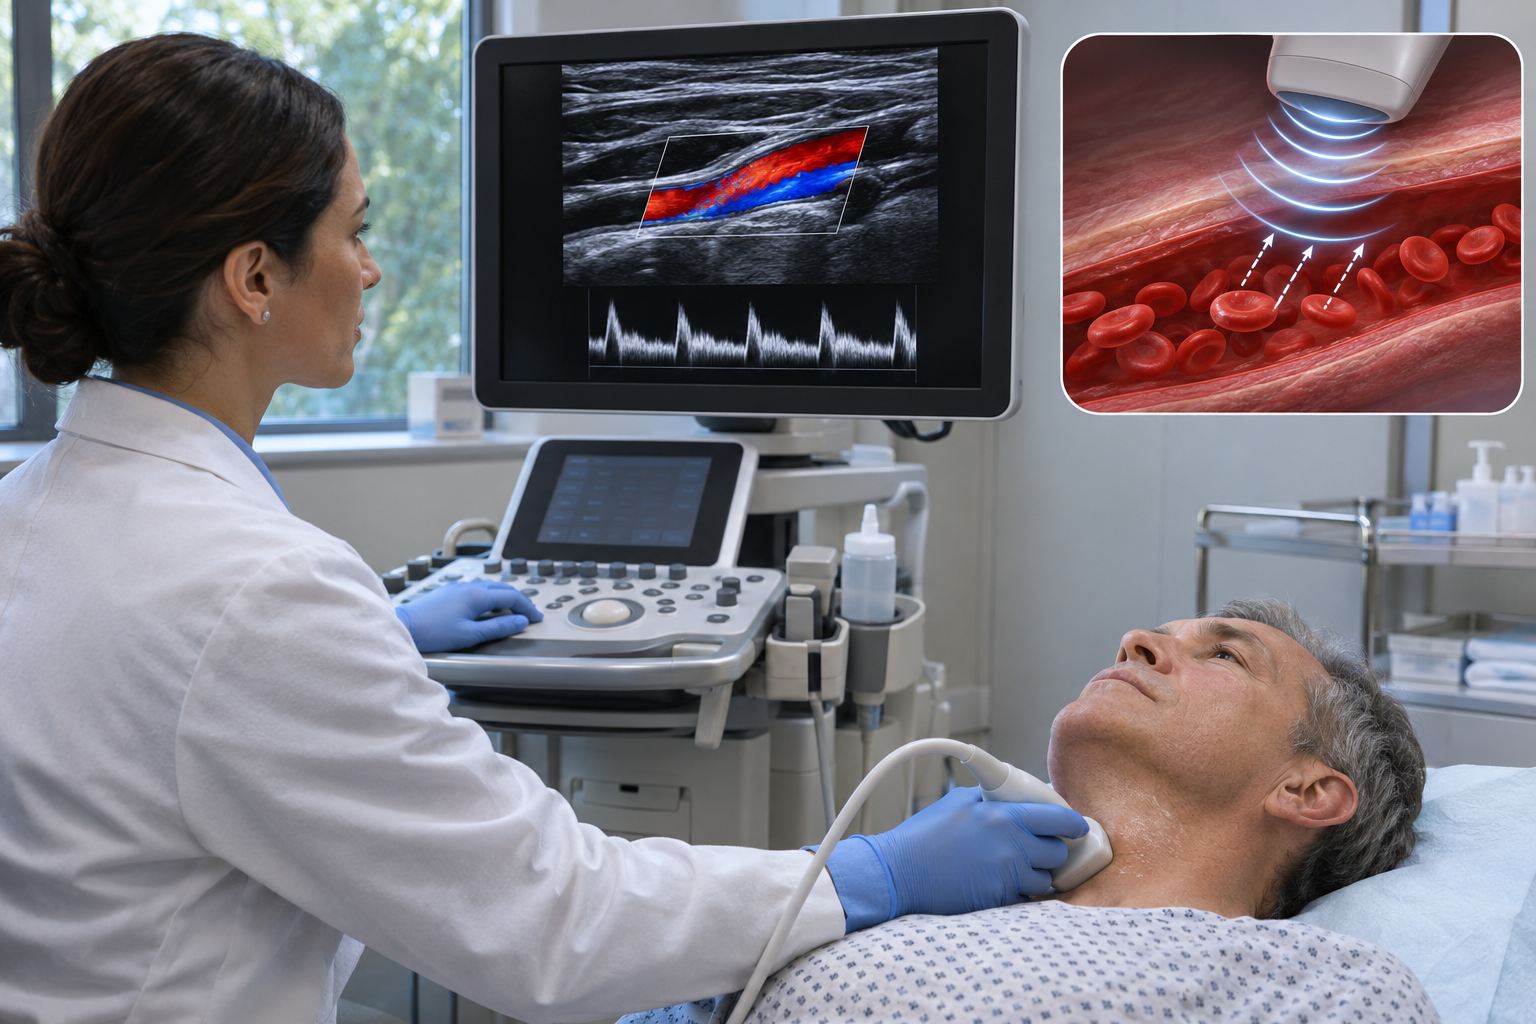
\includegraphics[width=\textwidth,keepaspectratio]{modalities/infographics/doppler_realistic.png}
\end{center}
\begin{center}\footnotesize Doppler measures frequency shifts from moving blood cells to estimate flow direction and velocity; angle and instrument settings affect the result. AI-generated illustration; displayed waveforms and images are illustrative.\end{center}

\section{Overview}
Doppler ultrasound is a specialized ultrasound imaging technique that evaluates the direction, velocity, and characteristics of blood flow through arteries, veins, and cardiac structures. It is particularly useful for identifying vascular obstruction, thrombosis, stenosis, abnormal vascular connections, and impaired tissue perfusion.

This catalogue focuses on diseases and conditions for which Doppler ultrasound provides clinically significant diagnostic information. It includes color Doppler, spectral Doppler, power Doppler, and duplex ultrasonography.

The 142 entries form a preliminary catalogue of diseases, conditions, and hemodynamic abnormalities. Doppler findings depend on acquisition angle, settings, physiologic state, and quantitative criteria. Absent flow does not always prove occlusion, and increased velocity or vascularity does not by itself establish stenosis or malignancy. Some findings require confirmatory imaging, laboratory testing, or clinical assessment.

\section{Where Doppler ultrasound is used}
The following numbered entries present common diagnostic applications by anatomical system. Findings are examples. Doppler measurements should be obtained with appropriate technique and interpreted with anatomy, clinical presentation, and relevant quantitative criteria. A technically limited or negative examination may not exclude disease.

\subsection{Carotid and cerebral circulation}
\begin{enumerate}[leftmargin=*,itemsep=0.45em,topsep=0.4em]
\item \textbf{Carotid artery dissection.} Useful imaging findings include: Possible intimal flap, mural hematoma, or abnormal flow; CTA or MRA may be needed.
\item \textbf{Carotid artery occlusion.} Useful imaging findings include: No detectable flow on a technically adequate examination; low flow or technical factors can mimic occlusion.
\item \textbf{Carotid artery stenosis.} Useful imaging findings include: Velocity criteria interpreted with plaque, waveform, and Doppler angle.
\item \textbf{Carotid atherosclerosis.} Useful imaging findings include: Plaque formation, disturbed blood flow.
\item \textbf{Cerebral circulatory arrest.} Useful imaging findings include: Characteristic waveforms may support assessment under a validated protocol; Doppler findings alone do not establish brain death.
\item \textbf{Cerebral vasospasm.} Useful imaging findings include: Elevated velocities interpreted with vessel ratios and clinical context; TCD is commonly used for monitoring after subarachnoid hemorrhage.
\item \textbf{Intracranial arterial stenosis.} Useful imaging findings include: Elevated velocities may indicate stenosis but depend on vessel, angle, flow state, and collateral circulation.
\item \textbf{Sickle cell cerebral vasculopathy.} Useful imaging findings include: TCD velocities are used for stroke-risk screening in children with sickle cell disease using validated protocols; thresholds are population- and protocol-specific.
\item \textbf{Subclavian steal syndrome.} Useful imaging findings include: Reversed vertebral arterial flow.
\item \textbf{Vertebral artery occlusion.} Useful imaging findings include: No detectable flow on a technically adequate study; confirm if the result changes management.
\item \textbf{Vertebral artery stenosis.} Useful imaging findings include: Focal velocity elevation with supportive waveform changes; limited visualization may require CTA or MRA.
\end{enumerate}

Intracranial blood flow is examined using transcranial Doppler (TCD).

\subsection{Peripheral arterial system}
\begin{enumerate}[leftmargin=*,itemsep=0.45em,topsep=0.4em]
\item \textbf{Acute limb ischemia.} Useful imaging findings include: Severely reduced or absent distal flow.
\item \textbf{Arterial aneurysm.} Useful imaging findings include: Arterial dilatation with altered flow patterns.
\item \textbf{Arterial bypass graft occlusion.} Useful imaging findings include: Absent graft flow.
\item \textbf{Arterial bypass graft stenosis.} Useful imaging findings include: Increased focal flow velocity.
\item \textbf{Arterial embolism.} Useful imaging findings include: Abrupt interruption of arterial flow.
\item \textbf{Arterial occlusion.} Useful imaging findings include: Absence of detectable blood flow.
\item \textbf{Arterial pseudoaneurysm.} Useful imaging findings include: To-and-fro spectral waveform.
\item \textbf{Arterial stenosis.} Useful imaging findings include: Focal increase in flow velocity.
\item \textbf{Arterial thrombosis.} Useful imaging findings include: Intraluminal thrombus with impaired flow.
\item \textbf{Arteriovenous fistula.} Useful imaging findings include: High-velocity turbulent flow.
\item \textbf{Arteriovenous malformation.} Useful imaging findings include: High-flow vascular channels.
\item \textbf{In-stent restenosis.} Useful imaging findings include: Elevated velocities using stent-specific criteria; native-vessel thresholds may overestimate stenosis.
\item \textbf{Peripheral arterial disease.} Useful imaging findings include: Monophasic waveforms, reduced distal perfusion.
\item \textbf{Popliteal artery entrapment syndrome.} Useful imaging findings include: Provocative maneuvers may reproduce flow reduction, which can also occur in asymptomatic people; correlate with symptoms and anatomic imaging.
\item \textbf{Thoracic outlet syndrome.} Useful imaging findings include: Positional compression may occur in asymptomatic people; interpret with symptoms and examination and distinguish arterial from venous disease.
\item \textbf{Thromboangiitis obliterans.} Useful imaging findings include: Distal segmental occlusions are nonspecific; diagnosis depends on clinical criteria and exclusion of other causes.
\end{enumerate}

\subsection{Peripheral venous system}
\begin{enumerate}[leftmargin=*,itemsep=0.45em,topsep=0.4em]
\item \textbf{Central venous stenosis.} Useful imaging findings include: Abnormal venous flow patterns.
\item \textbf{Chronic venous insufficiency.} Useful imaging findings include: Prolonged retrograde blood flow.
\item \textbf{Deep vein thrombosis (DVT).} Useful imaging findings include: Noncompressibility is the key finding. Doppler flow supports assessment but a negative limited study may require repeat or whole-leg ultrasound.
\item \textbf{Iliac vein thrombosis.} Useful imaging findings include: Abnormal or absent flow may raise suspicion, but pelvic veins can be difficult to visualize; CT or MR venography may be needed.
\item \textbf{Inferior vena cava thrombosis.} Useful imaging findings include: Visible thrombus or absent flow may support diagnosis; ultrasound can be limited by bowel gas and body habitus.
\item \textbf{May--Thurner syndrome.} Useful imaging findings include: Iliac vein compression and altered flow are supportive findings but compression is common without symptoms; assess for clinically significant obstruction and thrombosis.
\item \textbf{Paget--Schroetter syndrome.} Useful imaging findings include: Axillary-subclavian venous thrombosis.
\item \textbf{Post-thrombotic syndrome.} Useful imaging findings include: Residual obstruction and venous reflux.
\item \textbf{Superficial venous thrombosis.} Useful imaging findings include: Intraluminal thrombus.
\item \textbf{Upper extremity venous thrombosis.} Useful imaging findings include: Reduced flow and venous noncompressibility.
\item \textbf{Varicose veins.} Useful imaging findings include: Dilated superficial veins with reflux.
\item \textbf{Venous aneurysm.} Useful imaging findings include: Focal venous dilatation.
\item \textbf{Venous malformation.} Useful imaging findings include: Slow-flow vascular channels.
\end{enumerate}

\subsection{Hepatic and portal circulation}
\begin{enumerate}[leftmargin=*,itemsep=0.45em,topsep=0.4em]
\item \textbf{Budd--Chiari syndrome.} Useful imaging findings include: Hepatic venous outflow obstruction or collateral flow; technically limited examinations may need cross-sectional venography.
\item \textbf{Cavernous transformation of the portal vein.} Useful imaging findings include: Multiple collateral vascular channels.
\item \textbf{Congestive hepatopathy.} Useful imaging findings include: Increased portal venous pulsatility.
\item \textbf{Hepatic arteriovenous malformation.} Useful imaging findings include: Abnormal high-flow vascular connections.
\item \textbf{Hepatic artery stenosis.} Useful imaging findings include: Elevated focal velocity, tardus-parvus waveform.
\item \textbf{Hepatic artery thrombosis.} Useful imaging findings include: Absence of hepatic arterial flow.
\item \textbf{Hepatic vein thrombosis.} Useful imaging findings include: Absent flow or visible thrombus may support outflow obstruction. This overlaps with Budd--Chiari syndrome and is not a separate Doppler pattern.
\item \textbf{Portal hypertension.} Useful imaging findings include: Reversed portal flow or collaterals support portal hypertension; normal direction of flow does not exclude it.
\item \textbf{Portal vein thrombosis.} Useful imaging findings include: Absent or reduced portal flow.
\item \textbf{Splenic vein thrombosis.} Useful imaging findings include: Reduced or absent splenic venous flow.
\item \textbf{TIPS occlusion.} Useful imaging findings include: Absence of detectable shunt flow.
\item \textbf{TIPS stenosis.} Useful imaging findings include: Abnormal shunt velocities.
\end{enumerate}

\subsection{Renal circulation}
\begin{enumerate}[leftmargin=*,itemsep=0.45em,topsep=0.4em]
\item \textbf{Nutcracker syndrome.} Useful imaging findings include: Compression and velocity ratios may support the diagnosis but also occur without symptoms; clinical correlation is essential.
\item \textbf{Renal arteriovenous fistula.} Useful imaging findings include: Turbulent high-velocity flow.
\item \textbf{Renal artery aneurysm.} Useful imaging findings include: Focal vascular dilatation.
\item \textbf{Renal artery occlusion.} Useful imaging findings include: No detectable flow on an adequate examination; low flow and technical limitations can mimic occlusion.
\item \textbf{Renal artery pseudoaneurysm.} Useful imaging findings include: To-and-fro waveform.
\item \textbf{Renal artery stenosis.} Useful imaging findings include: Use validated velocity and renal-to-aortic ratio criteria with waveform assessment; a technically limited study may need CTA or MRA.
\item \textbf{Renal infarction.} Useful imaging findings include: Regional reduction in perfusion is nonspecific; contrast-enhanced CT or MRI is often needed to confirm.
\item \textbf{Renal vein thrombosis.} Useful imaging findings include: Visible thrombus or abnormal venous and arterial waveforms may support the diagnosis; confirm when technically limited.
\item \textbf{Transplant renal artery stenosis.} Useful imaging findings include: Elevated arterial flow velocity.
\item \textbf{Transplant renal vein thrombosis.} Useful imaging findings include: Absent venous flow, reversed arterial diastolic flow.
\end{enumerate}

\subsection{Abdominal and mesenteric circulation}
\begin{enumerate}[leftmargin=*,itemsep=0.45em,topsep=0.4em]
\item \textbf{Abdominal aortic aneurysm.} Useful imaging findings include: Aortic dilatation, possible mural thrombus.
\item \textbf{Abdominal aortic occlusion.} Useful imaging findings include: Absence of detectable aortic flow.
\item \textbf{Aortoiliac occlusive disease.} Useful imaging findings include: Abnormal aortoiliac flow velocities.
\item \textbf{Endoleak following aneurysm repair.} Useful imaging findings include: Doppler may detect sac flow, but a negative examination does not reliably exclude endoleak; CT angiography or other protocol imaging may be required.
\item \textbf{Median arcuate ligament syndrome.} Useful imaging findings include: Respiratory variation in celiac artery compression; anatomic compression is common in asymptomatic people and does not alone establish the syndrome.
\item \textbf{Mesenteric artery occlusion.} Useful imaging findings include: Absent or severely reduced arterial flow.
\item \textbf{Mesenteric artery stenosis.} Useful imaging findings include: Elevated velocities using validated criteria; fasting state, angle, and technical quality affect measurements.
\item \textbf{Mesenteric venous thrombosis.} Useful imaging findings include: Intraluminal thrombus, reduced venous flow.
\end{enumerate}

\subsection{Obstetric and fetal circulation}
\begin{enumerate}[leftmargin=*,itemsep=0.45em,topsep=0.4em]
\item \textbf{Fetal anemia.} Useful imaging findings include: MCA peak systolic velocity interpreted against gestational age; values above 1.5 MoM prompt specialist assessment, not a stand-alone diagnosis.
\item \textbf{Fetal arteriovenous malformation.} Useful imaging findings include: Abnormal high-flow vascular connections.
\item \textbf{Fetal cardiac compromise.} Useful imaging findings include: Abnormal ductus venosus waveforms indicate hemodynamic concern in selected high-risk pregnancies and require specialist interpretation.
\item \textbf{Fetal circulatory redistribution.} Useful imaging findings include: Low MCA resistance or cerebroplacental ratio may indicate redistribution; interpret with gestational age and the full growth assessment.
\item \textbf{Fetal growth restriction.} Useful imaging findings include: Umbilical artery resistance helps assess placental resistance and guide surveillance after growth restriction is identified; it does not establish FGR alone.
\item \textbf{Placenta accreta spectrum.} Useful imaging findings include: Abnormal lacunae and vascular patterns raise suspicion in an at-risk pregnancy; no individual sign excludes or confirms all cases.
\item \textbf{Placental insufficiency.} Useful imaging findings include: Abnormal waveforms support placental dysfunction in context; no single Doppler result establishes the diagnosis.
\item \textbf{Preeclampsia-associated placental dysfunction.} Useful imaging findings include: Increased uterine artery resistance is a risk marker, not a diagnostic test for preeclampsia.
\item \textbf{Twin anemia-polycythemia sequence.} Useful imaging findings include: Discordant MCA peak systolic velocities support diagnosis using validated intertwin criteria.
\item \textbf{Twin reversed arterial perfusion sequence.} Useful imaging findings include: Reversed arterial perfusion.
\item \textbf{Twin-to-twin transfusion syndrome.} Useful imaging findings include: Doppler findings contribute to staging and assessment; diagnosis also uses amniotic fluid and fetal findings in a monochorionic pregnancy.
\item \textbf{Umbilical artery thrombosis.} Useful imaging findings include: Absent flow in one artery may raise suspicion, but technical factors and cord anatomy must be assessed.
\item \textbf{Vasa previa.} Useful imaging findings include: Color and pulsed Doppler can confirm fetal vessels near or over the internal os; distinguish fetal from maternal vessels.
\item \textbf{Vein of Galen malformation.} Useful imaging findings include: High-flow intracranial vascular structure.
\end{enumerate}

\subsection{Female reproductive system}
\begin{enumerate}[leftmargin=*,itemsep=0.45em,topsep=0.4em]
\item \textbf{Corpus luteum cyst.} Useful imaging findings include: Prominent peripheral vascularity.
\item \textbf{Ectopic pregnancy.} Useful imaging findings include: Peripheral vascularity is nonspecific and also occurs around a corpus luteum; identify an extrauterine gestational sac or use serial clinical assessment.
\item \textbf{Endometrial polyp.} Useful imaging findings include: Single dominant feeding vessel.
\item \textbf{Ovarian carcinoma.} Useful imaging findings include: Internal vascularity in a complex mass can increase suspicion but is not specific for malignancy.
\item \textbf{Ovarian torsion.} Useful imaging findings include: Reduced flow supports torsion, but preserved flow does not exclude it because torsion may be partial or intermittent.
\item \textbf{Ovarian vein thrombosis.} Useful imaging findings include: Intraluminal thrombus, absent or reduced flow.
\item \textbf{Pelvic congestion syndrome.} Useful imaging findings include: Dilated pelvic veins with reflux.
\item \textbf{Retained products of conception.} Useful imaging findings include: Endometrial mass and vascularity support the diagnosis but overlap with other causes; correlate with symptoms and pregnancy history.
\item \textbf{Uterine arteriovenous malformation.} Useful imaging findings include: High-velocity, low-resistance flow.
\item \textbf{Uterine artery pseudoaneurysm.} Useful imaging findings include: To-and-fro waveform.
\item \textbf{Uterine fibroids.} Useful imaging findings include: Peripheral vascularity can be seen but varies with fibroid type and degeneration.
\end{enumerate}

Normal ovarian blood flow does not exclude ovarian torsion.

\subsection{Male reproductive system}
\begin{enumerate}[leftmargin=*,itemsep=0.45em,topsep=0.4em]
\item \textbf{Epididymitis.} Useful imaging findings include: Increased epididymal vascularity.
\item \textbf{Epididymo-orchitis.} Useful imaging findings include: Increased testicular and epididymal flow.
\item \textbf{High-flow priapism.} Useful imaging findings include: Increased cavernosal flow supports the diagnosis, often after trauma; interpret with clinical history and spectral measurements.
\item \textbf{Low-flow priapism.} Useful imaging findings include: Reduced cavernosal flow may be present, but urgent clinical assessment takes precedence and Doppler should not delay treatment.
\item \textbf{Orchitis.} Useful imaging findings include: Increased testicular vascularity.
\item \textbf{Testicular abscess.} Useful imaging findings include: Peripheral vascularity with avascular center.
\item \textbf{Testicular carcinoma.} Useful imaging findings include: A solid intratesticular mass is concerning; vascularity is variable and histology establishes tumor type.
\item \textbf{Testicular infarction.} Useful imaging findings include: Regional absence of perfusion.
\item \textbf{Testicular torsion.} Useful imaging findings include: Reduced flow and a twisted cord support torsion; preserved flow can occur in early, partial, or intermittent torsion.
\item \textbf{Varicocele.} Useful imaging findings include: Dilated veins with retrograde flow.
\item \textbf{Vasculogenic erectile dysfunction.} Useful imaging findings include: Penile duplex is performed after pharmacologic stimulation with protocol-specific measurements; resting flow alone is insufficient.
\end{enumerate}

\subsection{Cardiac Doppler echocardiography}
\begin{enumerate}[leftmargin=*,itemsep=0.45em,topsep=0.4em]
\item \textbf{Aortic regurgitation.} Useful imaging findings include: Retrograde diastolic blood flow.
\item \textbf{Aortic stenosis.} Useful imaging findings include: Increased transvalvular flow velocity.
\item \textbf{Atrial septal defect.} Useful imaging findings include: Abnormal interatrial flow.
\item \textbf{Cardiac tamponade.} Useful imaging findings include: Respiratory flow variation and chamber collapse support tamponade physiology, interpreted with clinical status and pericardial findings.
\item \textbf{Constrictive pericarditis.} Useful imaging findings include: Respiratory inflow variation supports constrictive physiology but overlaps with other conditions; combine with tissue Doppler and pericardial findings.
\item \textbf{Left ventricular diastolic dysfunction.} Useful imaging findings include: Tissue Doppler and transmitral flow are interpreted with left atrial and structural measures; no single velocity establishes filling pressure.
\item \textbf{Mitral regurgitation.} Useful imaging findings include: Retrograde systolic blood flow.
\item \textbf{Mitral stenosis.} Useful imaging findings include: Doppler-derived mean gradient depends on heart rate and flow; assess valve area and clinical context.
\item \textbf{Obstructive hypertrophic cardiomyopathy.} Useful imaging findings include: Increased left ventricular outflow velocity.
\item \textbf{Paravalvular leakage.} Useful imaging findings include: Abnormal flow around a prosthetic valve.
\item \textbf{Patent ductus arteriosus.} Useful imaging findings include: Persistent abnormal vascular flow.
\item \textbf{Prosthetic heart valve stenosis.} Useful imaging findings include: Elevated transprosthetic pressure gradient.
\item \textbf{Pulmonary hypertension.} Useful imaging findings include: Echocardiography estimates probability and pressure; right-heart catheterization confirms hemodynamics when required.
\item \textbf{Pulmonary valve regurgitation.} Useful imaging findings include: Retrograde diastolic flow.
\item \textbf{Pulmonary valve stenosis.} Useful imaging findings include: Increased transvalvular velocity.
\item \textbf{Tricuspid regurgitation.} Useful imaging findings include: Retrograde systolic blood flow.
\item \textbf{Tricuspid stenosis.} Useful imaging findings include: Doppler gradient depends on heart rate and flow; integrate valve morphology and other measurements.
\item \textbf{Ventricular septal defect.} Useful imaging findings include: Abnormal interventricular flow.
\end{enumerate}

\subsection{Inflammatory and musculoskeletal conditions}
\begin{enumerate}[leftmargin=*,itemsep=0.45em,topsep=0.4em]
\item \textbf{Active synovitis.} Useful imaging findings include: Increased synovial blood flow.
\item \textbf{Bursitis.} Useful imaging findings include: Increased peripheral vascularity.
\item \textbf{Cellulitis.} Useful imaging findings include: Increased subcutaneous blood flow.
\item \textbf{Enthesitis.} Useful imaging findings include: Increased vascularity at tendon insertions.
\item \textbf{Giant cell arteritis.} Useful imaging findings include: A noncompressible halo on temporal and axillary artery ultrasound supports diagnosis in trained hands; findings depend on timing and expertise and must be interpreted clinically.
\item \textbf{Psoriatic arthritis.} Useful imaging findings include: Synovial and entheseal hypervascularity.
\item \textbf{Rheumatoid arthritis.} Useful imaging findings include: Increased synovial vascularity.
\item \textbf{Soft-tissue abscess.} Useful imaging findings include: Peripheral hypervascularity.
\item \textbf{Tendinopathy.} Useful imaging findings include: Abnormal intratendinous neovascularization.
\item \textbf{Tenosynovitis.} Useful imaging findings include: Increased tendon sheath vascularity.
\end{enumerate}

\subsection{Thyroid and breast conditions}
\begin{enumerate}[leftmargin=*,itemsep=0.45em,topsep=0.4em]
\item \textbf{Breast abscess.} Useful imaging findings include: Peripheral hypervascularity.
\item \textbf{Breast carcinoma.} Useful imaging findings include: Doppler vascularity is nonspecific; grayscale morphology and clinical findings guide assessment, and biopsy establishes histology.
\item \textbf{Graves disease.} Useful imaging findings include: Diffuse hypervascularity can support Graves disease but is not specific; thyroid function and antibody tests establish the clinical diagnosis.
\item \textbf{Hashimoto thyroiditis.} Useful imaging findings include: Variable thyroid vascularity.
\item \textbf{Intraductal papilloma.} Useful imaging findings include: A vascular stalk supports an intraductal mass but is not specific; pathology may be needed depending on imaging and clinical findings.
\item \textbf{Mastitis.} Useful imaging findings include: Hyperemia can support inflammation but overlaps with other causes; assess for abscess and correlate with symptoms.
\item \textbf{Parathyroid adenoma.} Useful imaging findings include: Prominent polar feeding vessel.
\item \textbf{Thyroid nodules.} Useful imaging findings include: Doppler vascularity alone does not reliably distinguish benign from malignant nodules; use validated grayscale risk stratification and biopsy criteria.
\end{enumerate}

\subsection{Summary}
\begin{center}
\begin{tabular}{@{}p{0.70\textwidth}r@{}}
\toprule
\textbf{Disease category} & \textbf{Entries} \\
\midrule
Anatomical system & Conditions \\
Abdominal and mesenteric circulation & 8 \\
Cardiac Doppler echocardiography & 18 \\
Carotid and cerebral circulation & 11 \\
Female reproductive system & 11 \\
Hepatic and portal circulation & 12 \\
Inflammatory and musculoskeletal conditions & 10 \\
Male reproductive system & 11 \\
Obstetric and fetal circulation & 14 \\
Peripheral arterial system & 16 \\
Peripheral venous system & 13 \\
Renal circulation & 10 \\
Thyroid and breast conditions & 8 \\
Total & 142 \\
\bottomrule
\end{tabular}
\end{center}

\subsection{Types of Doppler imaging}
\begin{longtable}{@{}p{0.34\textwidth}p{0.60\textwidth}@{}}
\toprule
\textbf{Technique} & \textbf{Primary diagnostic application} \\
\midrule
\endfirsthead
\toprule
\textbf{Technique} & \textbf{Primary diagnostic application} \\
\midrule
\endhead
Color Doppler & Blood flow distribution and direction \\
Continuous-wave Doppler & Measurement of high-velocity blood flow \\
Duplex ultrasound & Combined grayscale imaging and Doppler assessment \\
Power Doppler & Detection of slow blood flow \\
Pulsed-wave Doppler & Flow velocity measurement at a specific location \\
Tissue Doppler & Measurement of myocardial tissue velocity \\
Transcranial Doppler & Intracranial blood flow assessment \\
Triplex ultrasound & Grayscale, color, and spectral Doppler \\
\bottomrule
\end{longtable}

\subsection{Authoritative medical sources}
\begin{longtable}{@{}p{0.40\textwidth}p{0.54\textwidth}@{}}
\toprule
\textbf{Source} & \textbf{Primary utility} \\
\midrule
\endfirsthead
\toprule
\textbf{Source} & \textbf{Primary utility} \\
\midrule
\endhead
ACR Appropriateness Criteria & Clinical indications for imaging \\
American Institute of Ultrasound in Medicine & Ultrasound practice parameters \\
American Society of Echocardiography & Cardiac Doppler imaging \\
International Society of Ultrasound in Obstetrics and Gynecology & Maternal and fetal Doppler imaging \\
PubMed Central & Published clinical images \\
Radiopaedia & Annotated clinical Doppler images \\
Society for Vascular Ultrasound & Vascular diagnostic protocols \\
\bottomrule
\end{longtable}

\subsection{Recommended metadata for a medical imaging dataset}
Unlike conventional ultrasound, Doppler imaging provides quantitative hemodynamic information. The following measurements and descriptors can be captured as dataset metadata:

\begin{longtable}{@{}p{0.56\textwidth}p{0.38\textwidth}@{}}
\toprule
\textbf{Parameter} & \textbf{Abbreviation} \\
\midrule
\endfirsthead
\toprule
\textbf{Parameter} & \textbf{Abbreviation} \\
\midrule
\endhead
Acceleration time & AT \\
End-diastolic velocity & EDV \\
Flow direction & --- \\
Mean flow velocity & MFV \\
Peak systolic velocity & PSV \\
Pressure gradient & PG \\
Pulsatility index & PI \\
Resistive index & RI \\
Spectral waveform morphology & --- \\
Systolic-to-diastolic ratio & S/D \\
Venous reflux duration & --- \\
Volume flow rate & --- \\
\bottomrule
\end{longtable}

The 142 entries constitute a preliminary catalogue of diseases, conditions, and hemodynamic abnormalities. Some overlap, and several require additional imaging or clinical confirmation. Tumor vascularity, in particular, is not independently diagnostic of malignancy.

For establishing diagnostic ground truth, individual clinical guideline verification and quantitative Doppler measurements are preferable to relying exclusively on static images.

\chapter{Echocardiography}
\label{ch:echocardiography}

% Chapter-opening illustrated modality infographic.
\begin{center}
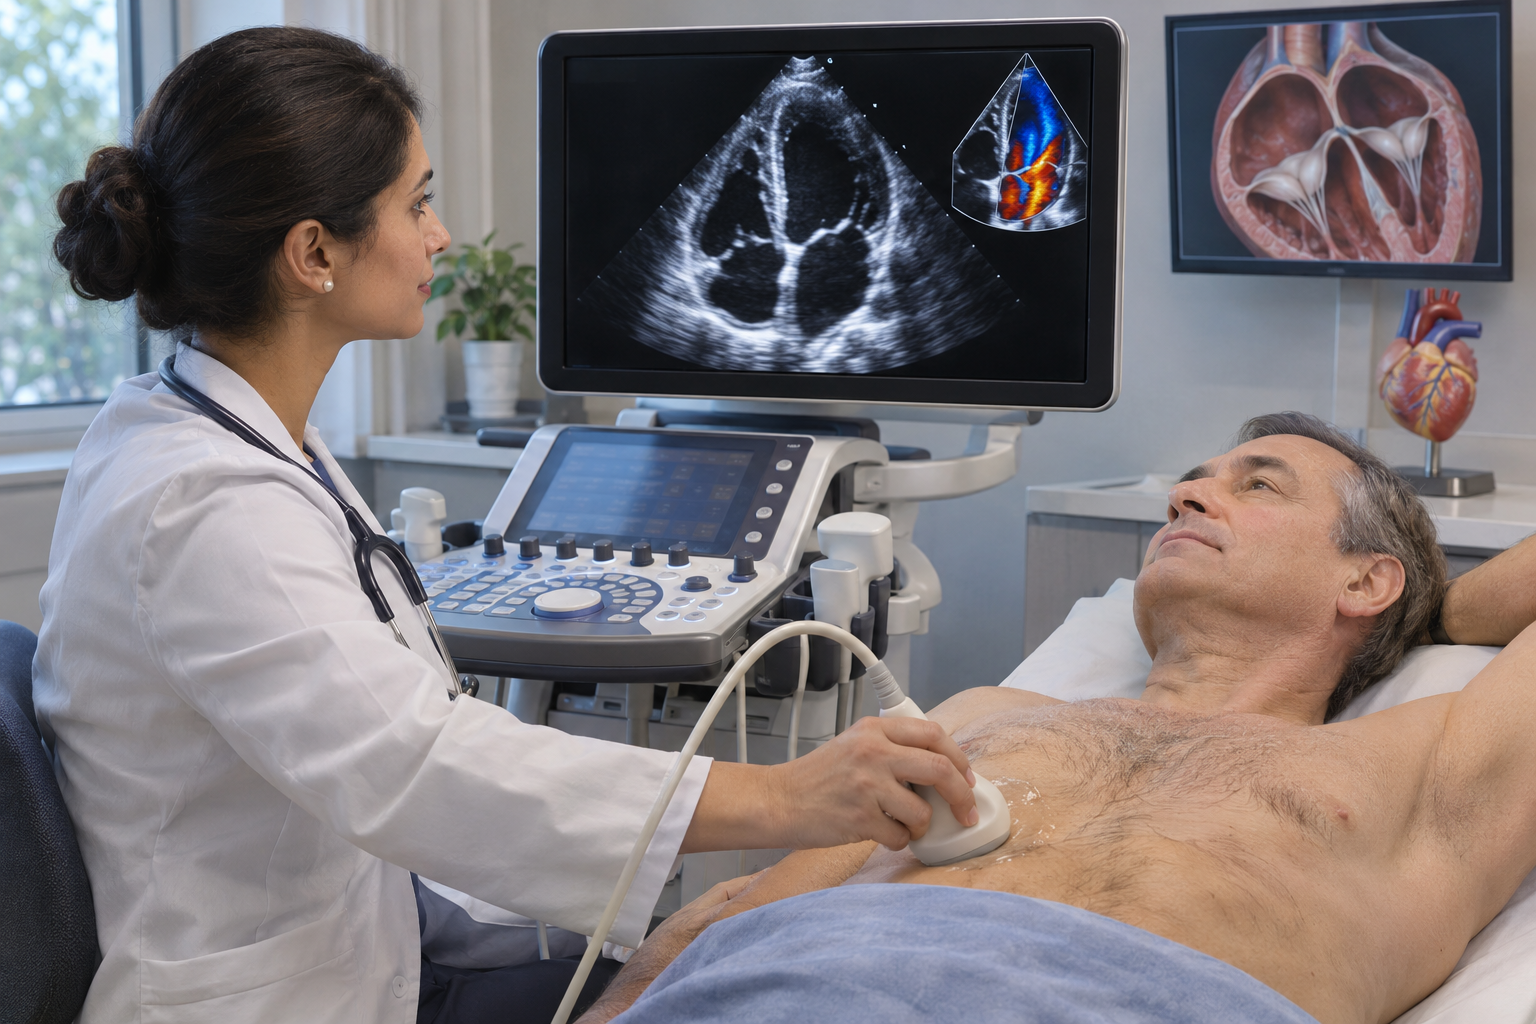
\includegraphics[width=\textwidth,keepaspectratio]{modalities/infographics/echocardiography_realistic.png}
\end{center}
\begin{center}\footnotesize Echocardiography uses ultrasound views and Doppler to assess cardiac structure, motion, and blood flow; measurements require clinical context. AI-generated illustration; echo panels are not clinical studies.\end{center}

\section{Overview}
Echocardiography is a specialized ultrasound imaging technique that evaluates cardiac anatomy, myocardial function, valvular function, intracardiac blood flow, and hemodynamics. It is one of the principal diagnostic imaging modalities used in cardiology.

This catalogue focuses on diseases and conditions for which echocardiography has established clinical utility. It includes transthoracic echocardiography (TTE), transesophageal echocardiography (TEE), stress echocardiography, Doppler echocardiography, and three-dimensional echocardiography.

\section{Where echocardiography is used}
The following numbered entries present common diagnostic applications by disease category. Findings should be interpreted with clinical information, appropriate views, and quantitative measurements.

\subsection{Cardiomyopathies}
\begin{enumerate}[leftmargin=*,itemsep=0.45em,topsep=0.4em]
\item \textbf{Alcohol-induced cardiomyopathy.} Useful imaging findings include: Ventricular dilatation and systolic dysfunction.
\item \textbf{Arrhythmogenic right ventricular cardiomyopathy.} Useful imaging findings include: Right ventricular dilatation and regional dysfunction.
\item \textbf{Cardiac amyloidosis.} Useful imaging findings include: Increased wall thickness and relative apical strain sparing may raise suspicion but are not diagnostic or subtype-specific.
\item \textbf{Cardiac sarcoidosis.} Useful imaging findings include: Regional dysfunction, basal septal thinning.
\item \textbf{Chemotherapy-induced cardiomyopathy.} Useful imaging findings include: Reduced ejection fraction or global longitudinal strain.
\item \textbf{Dilated cardiomyopathy.} Useful imaging findings include: Ventricular dilatation, reduced systolic function.
\item \textbf{Endomyocardial fibrosis.} Useful imaging findings include: Apical obliteration and restrictive filling.
\item \textbf{Hypertensive heart disease.} Useful imaging findings include: Left ventricular hypertrophy, diastolic dysfunction.
\item \textbf{Hypertrophic cardiomyopathy.} Useful imaging findings include: Abnormal myocardial hypertrophy.
\item \textbf{Hypertrophic obstructive cardiomyopathy.} Useful imaging findings include: Left ventricular outflow tract obstruction.
\item \textbf{Ischemic cardiomyopathy.} Useful imaging findings include: Regional wall-motion abnormalities.
\item \textbf{Left ventricular noncompaction.} Useful imaging findings include: Prominent trabeculations; interpret with ventricular function and clinical context, since trabeculation alone is not diagnostic.
\item \textbf{Peripartum cardiomyopathy.} Useful imaging findings include: Reduced left ventricular systolic function.
\item \textbf{Restrictive cardiomyopathy.} Useful imaging findings include: Restrictive ventricular filling pattern.
\item \textbf{Takotsubo cardiomyopathy.} Useful imaging findings include: Transient regional ventricular ballooning.
\end{enumerate}

\subsection{Valvular heart diseases}
\begin{enumerate}[leftmargin=*,itemsep=0.45em,topsep=0.4em]
\item \textbf{Aortic regurgitation.} Useful imaging findings include: Retrograde diastolic flow.
\item \textbf{Aortic stenosis.} Useful imaging findings include: Restricted leaflet opening, elevated pressure gradient.
\item \textbf{Bicuspid aortic valve.} Useful imaging findings include: Two functional aortic valve cusps.
\item \textbf{Carcinoid heart disease.} Useful imaging findings include: Thickened, retracted right-sided valve leaflets.
\item \textbf{Chordae tendineae rupture.} Useful imaging findings include: Disrupted chordal support with leaflet flail.
\item \textbf{Flail mitral leaflet.} Useful imaging findings include: Abnormal leaflet motion into the left atrium.
\item \textbf{Mitral annular calcification.} Useful imaging findings include: Echogenic calcification of the mitral annulus.
\item \textbf{Mitral regurgitation.} Useful imaging findings include: Retrograde systolic flow.
\item \textbf{Mitral stenosis.} Useful imaging findings include: Restricted leaflet opening, reduced valve area.
\item \textbf{Mitral valve prolapse.} Useful imaging findings include: Systolic displacement of mitral leaflets.
\item \textbf{Papillary muscle rupture.} Useful imaging findings include: Papillary muscle disruption, severe mitral regurgitation.
\item \textbf{Paravalvular leakage.} Useful imaging findings include: Regurgitant flow surrounding the prosthetic valve.
\item \textbf{Prosthetic valve regurgitation.} Useful imaging findings include: Abnormal regurgitant flow.
\item \textbf{Prosthetic valve stenosis.} Useful imaging findings include: Elevated transprosthetic pressure gradient; interpret with flow, valve type and size, and other Doppler measures.
\item \textbf{Prosthetic valve thrombosis.} Useful imaging findings include: Restricted prosthetic leaflet motion.
\item \textbf{Pulmonary valve regurgitation.} Useful imaging findings include: Retrograde diastolic flow.
\item \textbf{Pulmonary valve stenosis.} Useful imaging findings include: Elevated transpulmonary flow velocity.
\item \textbf{Rheumatic heart disease.} Useful imaging findings include: Leaflet thickening, commissural fusion.
\item \textbf{Tricuspid regurgitation.} Useful imaging findings include: Retrograde systolic flow.
\item \textbf{Tricuspid stenosis.} Useful imaging findings include: Restricted valve opening, increased pressure gradient.
\end{enumerate}

\subsection{Heart failure and ventricular dysfunction}
\begin{enumerate}[leftmargin=*,itemsep=0.45em,topsep=0.4em]
\item \textbf{Biventricular dysfunction.} Useful imaging findings include: Impaired function of both ventricles.
\item \textbf{Heart failure with mildly reduced ejection fraction (HFmrEF).} Useful imaging findings include: Mildly reduced ejection fraction.
\item \textbf{Heart failure with preserved ejection fraction (HFpEF).} Useful imaging findings include: Preserved ejection fraction; diastolic measures can support but do not establish the diagnosis without clinical context.
\item \textbf{Heart failure with reduced ejection fraction (HFrEF).} Useful imaging findings include: Reduced left ventricular ejection fraction.
\item \textbf{Left atrial enlargement.} Useful imaging findings include: Increased left atrial volume.
\item \textbf{Left ventricular diastolic dysfunction.} Useful imaging findings include: Abnormal ventricular relaxation and filling.
\item \textbf{Left ventricular dilatation.} Useful imaging findings include: Increased ventricular chamber dimensions.
\item \textbf{Left ventricular hypertrophy.} Useful imaging findings include: Increased myocardial wall thickness or mass.
\item \textbf{Right atrial enlargement.} Useful imaging findings include: Increased right atrial dimensions.
\item \textbf{Right ventricular dilatation.} Useful imaging findings include: Enlarged right ventricular chamber.
\item \textbf{Right ventricular failure.} Useful imaging findings include: Reduced right ventricular systolic function.
\item \textbf{Right ventricular hypertrophy.} Useful imaging findings include: Increased right ventricular wall thickness.
\end{enumerate}

\subsection{Ischemic heart disease}
\begin{enumerate}[leftmargin=*,itemsep=0.45em,topsep=0.4em]
\item \textbf{Acute myocardial infarction.} Useful imaging findings include: Regional wall-motion abnormalities.
\item \textbf{Hibernating myocardium.} Useful imaging findings include: Dysfunctional myocardium with contractile reserve.
\item \textbf{Ischemic mitral regurgitation.} Useful imaging findings include: Leaflet tethering and regurgitant flow.
\item \textbf{Left ventricular aneurysm.} Useful imaging findings include: Dyskinetic ventricular outpouching.
\item \textbf{Left ventricular free-wall rupture.} Useful imaging findings include: Myocardial disruption, hemopericardium.
\item \textbf{Left ventricular pseudoaneurysm.} Useful imaging findings include: Contained ventricular rupture.
\item \textbf{Myocardial ischemia.} Useful imaging findings include: Inducible wall-motion abnormalities during stress.
\item \textbf{Previous myocardial infarction.} Useful imaging findings include: Regional myocardial thinning and akinesia.
\item \textbf{Stunned myocardium.} Useful imaging findings include: Transient myocardial contractile dysfunction.
\item \textbf{Ventricular septal rupture.} Useful imaging findings include: Acquired interventricular communication.
\end{enumerate}

\subsection{Pericardial diseases}
\begin{enumerate}[leftmargin=*,itemsep=0.45em,topsep=0.4em]
\item \textbf{Cardiac tamponade.} Useful imaging findings include: Right-sided chamber collapse and respiratory flow variation.
\item \textbf{Congenital absence of the pericardium.} Useful imaging findings include: Abnormal cardiac position and mobility.
\item \textbf{Constrictive pericarditis.} Useful imaging findings include: Septal bounce and ventricular interdependence.
\item \textbf{Effusive-constrictive pericarditis.} Useful imaging findings include: Pericardial fluid with constrictive physiology.
\item \textbf{Hemopericardium.} Useful imaging findings include: Pericardial fluid, sometimes with echogenic clot.
\item \textbf{Pericardial cyst.} Useful imaging findings include: Extracardiac cystic structure.
\item \textbf{Pericardial effusion.} Useful imaging findings include: Echo-free space surrounding the heart.
\end{enumerate}

\subsection{Congenital heart diseases}
\begin{enumerate}[leftmargin=*,itemsep=0.45em,topsep=0.4em]
\item \textbf{Anomalous left coronary artery from pulmonary artery (ALCAPA).} Useful imaging findings include: Abnormal coronary origin and flow.
\item \textbf{Aortic valve atresia.} Useful imaging findings include: Absent direct flow through the aortic valve.
\item \textbf{Atrial septal defect (ASD).} Useful imaging findings include: Interatrial communication.
\item \textbf{Atrioventricular septal defect.} Useful imaging findings include: Abnormal atrioventricular junction and septal defects.
\item \textbf{Coarctation of the aorta.} Useful imaging findings include: Aortic narrowing with accelerated blood flow.
\item \textbf{Congenital coronary artery fistula.} Useful imaging findings include: Abnormal coronary vascular communication.
\item \textbf{Congenital corrected transposition.} Useful imaging findings include: Atrioventricular and ventriculoarterial discordance.
\item \textbf{Congenital submitral aneurysm.} Useful imaging findings include: Ventricular outpouching beneath the mitral annulus.
\item \textbf{Cor triatriatum.} Useful imaging findings include: Abnormal membrane dividing an atrial chamber.
\item \textbf{Double-outlet right ventricle.} Useful imaging findings include: Both great arteries arising predominantly from the right ventricle.
\item \textbf{Ebstein anomaly.} Useful imaging findings include: Apical displacement of tricuspid valve leaflets.
\item \textbf{Hypoplastic left heart syndrome.} Useful imaging findings include: Underdeveloped left-sided cardiac structures.
\item \textbf{Interrupted aortic arch.} Useful imaging findings include: Discontinuity of the aortic arch.
\item \textbf{Partial anomalous pulmonary venous return.} Useful imaging findings include: Partial abnormal pulmonary venous drainage.
\item \textbf{Patent ductus arteriosus (PDA).} Useful imaging findings include: Persistent communication between aorta and pulmonary artery.
\item \textbf{Patent foramen ovale (PFO).} Useful imaging findings include: Interatrial shunting, often demonstrated with bubble study.
\item \textbf{Persistent left superior vena cava.} Useful imaging findings include: Dilated coronary sinus, abnormal venous drainage.
\item \textbf{Pulmonary atresia.} Useful imaging findings include: Absent direct flow through the pulmonary valve.
\item \textbf{Sinus of Valsalva aneurysm.} Useful imaging findings include: Abnormal aortic sinus dilatation.
\item \textbf{Tetralogy of Fallot.} Useful imaging findings include: VSD, overriding aorta, right ventricular outflow obstruction and hypertrophy.
\item \textbf{Total anomalous pulmonary venous return.} Useful imaging findings include: Abnormal pulmonary venous drainage.
\item \textbf{Transposition of the great arteries.} Useful imaging findings include: Ventriculoarterial discordance.
\item \textbf{Tricuspid atresia.} Useful imaging findings include: Absent functional tricuspid valve opening.
\item \textbf{Truncus arteriosus.} Useful imaging findings include: Single common arterial trunk.
\item \textbf{Ventricular septal defect (VSD).} Useful imaging findings include: Interventricular communication.
\end{enumerate}

\subsection{Cardiac infections and inflammatory diseases}
\begin{enumerate}[leftmargin=*,itemsep=0.45em,topsep=0.4em]
\item \textbf{Cardiac fistula associated with endocarditis.} Useful imaging findings include: Abnormal intracardiac flow communication.
\item \textbf{Infective endocarditis.} Useful imaging findings include: Possible vegetations or complications; a negative TTE does not exclude disease when clinical suspicion remains.
\item \textbf{Libman--Sacks endocarditis.} Useful imaging findings include: Sterile valvular vegetations.
\item \textbf{Myocarditis.} Useful imaging findings include: Global or regional ventricular dysfunction.
\item \textbf{Nonbacterial thrombotic endocarditis.} Useful imaging findings include: Sterile valvular masses.
\item \textbf{Perivalvular abscess.} Useful imaging findings include: Abnormal perivalvular cavity or thickening.
\item \textbf{Prosthetic valve endocarditis.} Useful imaging findings include: Possible vegetation, prosthetic dysfunction or dehiscence; prosthetic shadowing can limit TTE and TEE.
\item \textbf{Rheumatic carditis.} Useful imaging findings include: Valvular inflammation and regurgitation.
\end{enumerate}

\subsection{Intracardiac tumors and masses}
\begin{enumerate}[leftmargin=*,itemsep=0.45em,topsep=0.4em]
\item \textbf{Atrial myxoma.} Useful imaging findings include: Mobile intracavitary mass.
\item \textbf{Cardiac angiosarcoma.} Useful imaging findings include: Irregular infiltrative mass.
\item \textbf{Cardiac fibroma.} Useful imaging findings include: Solid intramyocardial mass.
\item \textbf{Cardiac lipoma.} Useful imaging findings include: Well-defined cardiac mass.
\item \textbf{Cardiac lymphoma.} Useful imaging findings include: Infiltrative myocardial or intracardiac mass.
\item \textbf{Cardiac metastases.} Useful imaging findings include: Abnormal myocardial or pericardial masses.
\item \textbf{Cardiac papillary fibroelastoma.} Useful imaging findings include: Small mobile valvular mass.
\item \textbf{Cardiac rhabdomyoma.} Useful imaging findings include: Intramyocardial masses.
\item \textbf{Lambl excrescences.} Useful imaging findings include: Thin filamentous valvular structures.
\item \textbf{Left atrial appendage thrombus.} Useful imaging findings include: Intracavitary mass visualized predominantly with TEE.
\item \textbf{Left atrial thrombus.} Useful imaging findings include: Mass within the left atrium.
\item \textbf{Left ventricular thrombus.} Useful imaging findings include: Intracavitary mass, frequently near the apex.
\item \textbf{Right atrial thrombus.} Useful imaging findings include: Intracavitary right atrial mass.
\item \textbf{Right ventricular thrombus.} Useful imaging findings include: Intracavitary right ventricular mass.
\end{enumerate}

\subsection{Aortic diseases}
\begin{enumerate}[leftmargin=*,itemsep=0.45em,topsep=0.4em]
\item \textbf{Aortic annuloectasia.} Useful imaging findings include: Dilatation of the aortic annulus and root.
\item \textbf{Aortic atherosclerosis.} Useful imaging findings include: Echogenic aortic plaques.
\item \textbf{Aortic dissection.} Useful imaging findings include: Intimal flap may be seen in accessible segments; echocardiography does not assess the entire aorta.
\item \textbf{Aortic intramural hematoma.} Useful imaging findings include: Possible aortic wall thickening; findings are nonspecific and CT or MRI is generally needed.
\item \textbf{Aortic root abscess.} Useful imaging findings include: Abnormal periannular cavity.
\item \textbf{Aortic root dilatation.} Useful imaging findings include: Increased aortic root diameter.
\item \textbf{Ascending aortic aneurysm.} Useful imaging findings include: Enlarged ascending aorta.
\end{enumerate}

\subsection{Pulmonary circulation}
\begin{enumerate}[leftmargin=*,itemsep=0.45em,topsep=0.4em]
\item \textbf{Acute pulmonary embolism.} Useful imaging findings include: Possible right ventricular strain or dilatation; a normal echocardiogram does not exclude PE.
\item \textbf{Chronic thromboembolic pulmonary hypertension.} Useful imaging findings include: Right ventricular hypertrophy and pressure overload; echocardiography does not identify the thromboembolic obstruction.
\item \textbf{Cor pulmonale.} Useful imaging findings include: Right ventricular structural and functional abnormalities.
\item \textbf{Eisenmenger syndrome.} Useful imaging findings include: Pulmonary hypertension with bidirectional or reversed shunting.
\item \textbf{Pulmonary artery aneurysm.} Useful imaging findings include: Pulmonary artery dilatation.
\item \textbf{Pulmonary artery stenosis.} Useful imaging findings include: Localized flow acceleration.
\item \textbf{Pulmonary hypertension.} Useful imaging findings include: Elevated estimated pulmonary pressure; echocardiography estimates probability and does not replace catheter confirmation when indicated.
\end{enumerate}

Echocardiography can demonstrate the hemodynamic consequences of pulmonary embolism but cannot reliably exclude it.

When endocarditis remains clinically suspected despite a nondiagnostic study, additional imaging, often TEE, may be required. The choice depends on the patient, suspected complication, and initial image quality.

\subsection{Postoperative and device-related conditions}
\begin{enumerate}[leftmargin=*,itemsep=0.45em,topsep=0.4em]
\item \textbf{Cardiac device-related perforation.} Useful imaging findings include: Abnormal lead position, possible pericardial effusion.
\item \textbf{Left atrial appendage occluder leakage.} Useful imaging findings include: Residual flow around the occlusion device.
\item \textbf{Left ventricular assist device obstruction.} Useful imaging findings include: Abnormal cannula flow characteristics.
\item \textbf{Pacemaker lead-associated endocarditis.} Useful imaging findings include: Vegetation attached to intracardiac lead.
\item \textbf{Pacemaker lead-associated thrombus.} Useful imaging findings include: Mass attached to intracardiac lead.
\item \textbf{Prosthetic valve dehiscence.} Useful imaging findings include: Abnormal rocking motion of prosthetic valve.
\item \textbf{Residual atrial septal defect.} Useful imaging findings include: Persistent interatrial shunting.
\item \textbf{Residual ventricular septal defect.} Useful imaging findings include: Persistent interventricular shunting.
\end{enumerate}

\subsection{Summary}
\begin{center}
\begin{tabular}{@{}p{0.70\textwidth}r@{}}
\toprule
\textbf{Disease category} & \textbf{Entries} \\
\midrule
Aortic diseases & 7 \\
Cardiomyopathies & 15 \\
Congenital heart diseases & 25 \\
Heart failure and ventricular dysfunction & 12 \\
Infections and inflammatory diseases & 8 \\
Intracardiac tumors and masses & 14 \\
Ischemic heart disease & 10 \\
Pericardial diseases & 7 \\
Postoperative and device-related conditions & 8 \\
Pulmonary circulation & 7 \\
Valvular heart diseases & 20 \\
\midrule
\textbf{Total} & \textbf{133} \\
\bottomrule
\end{tabular}
\end{center}

\subsection{Types of echocardiography}
\begin{longtable}{@{}p{0.40\textwidth}p{0.54\textwidth}@{}}
\toprule
\textbf{Technique} & \textbf{Primary diagnostic application} \\
\midrule
\endfirsthead
\toprule
\textbf{Technique} & \textbf{Primary diagnostic application} \\
\midrule
\endhead
2D echocardiography & Structural cardiac abnormalities \\
3D echocardiography & Volumetric and complex anatomical assessment \\
Color Doppler echocardiography & Abnormal intracardiac blood flow \\
Contrast echocardiography & Chamber delineation and shunt assessment \\
Fetal echocardiography & Congenital cardiac abnormalities \\
M-mode echocardiography & Cardiac dimensions and tissue motion \\
Speckle-tracking echocardiography & Myocardial deformation and strain \\
Spectral Doppler echocardiography & Flow velocities and pressure gradients \\
Stress echocardiography & Inducible myocardial ischemia \\
Tissue Doppler imaging & Myocardial tissue velocities \\
Transesophageal echocardiography (TEE) & Detailed valvular and intracardiac examination \\
Transthoracic echocardiography (TTE) & Routine cardiac structural and functional assessment \\
\bottomrule
\end{longtable}

\subsection{Quantitative parameters}
For developing an echocardiographic medical imaging dataset, the following measurements are particularly important.

\begin{longtable}{@{}p{0.64\textwidth}p{0.30\textwidth}@{}}
\toprule
\textbf{Parameter} & \textbf{Abbreviation} \\
\midrule
\endfirsthead
\toprule
\textbf{Parameter} & \textbf{Abbreviation} \\
\midrule
\endhead
Aortic valve area & AVA \\
Cardiac index & CI \\
Cardiac output & CO \\
Early-to-late transmitral flow velocity ratio & E/A \\
Effective regurgitant orifice area & EROA \\
Global longitudinal strain & GLS \\
Left atrial volume index & LAVI \\
Left ventricular ejection fraction & LVEF \\
Left ventricular end-diastolic volume & LVEDV \\
Left ventricular end-systolic volume & LVESV \\
Left ventricular mass index & LVMI \\
Mitral valve area & MVA \\
Pulmonary artery systolic pressure & PASP \\
Regurgitant fraction & RF \\
Regurgitant volume & RVol \\
Right ventricular fractional area change & RVFAC \\
Stroke volume & SV \\
Transmitral-to-annular early diastolic velocity ratio & E/e$^{\prime}$ \\
Tricuspid annular plane systolic excursion & TAPSE \\
\bottomrule
\end{longtable}

\subsection{Published medical images and datasets}
\begin{longtable}{@{}p{0.40\textwidth}p{0.54\textwidth}@{}}
\toprule
\textbf{Source} & \textbf{Primary utility} \\
\midrule
\endfirsthead
\toprule
\textbf{Source} & \textbf{Primary utility} \\
\midrule
\endhead
American Society of Echocardiography & Clinical guidelines and diagnostic criteria \\
CAMUS Dataset & Cardiac ultrasound segmentation \\
EchoNet-Dynamic & Annotated echocardiographic videos \\
Echopedia & Educational echocardiographic images \\
European Association of Cardiovascular Imaging & Cardiovascular imaging standards \\
PubMed Central & Published clinical images and videos \\
Radiopaedia & Clinical imaging cases \\
\bottomrule
\end{longtable}

\subsection{Selected clinical guidance}
The following professional guidance supports interpretation of the findings and limitations summarized in this chapter:
\begin{itemize}
\item \href{https://academic.oup.com/eurheartj/article/44/37/3503/7246608}{2023 ESC Guidelines for the management of cardiomyopathies} (trabeculation and cardiomyopathy assessment).
\item \href{https://ashpublications.org/bloodadvances/article/doi/10.1182/bloodadvances.2025017073/566264}{ASH clinical practice guidance on diagnosis of light-chain amyloidosis} (cardiac findings require etiologic confirmation).
\item \href{https://academic.oup.com/eurheartj/article/44/39/3948/7243107}{2023 ESC Guidelines for the management of endocarditis} (multimodality imaging and prosthetic-valve limitations).
\item \href{https://www.asecho.org/wp-content/uploads/2025/07/Left-Ventricular-Diastolic-Function.pdf}{ASE 2025 recommendations for evaluation of left ventricular diastolic function}.
\item \href{https://www.asecho.org/wp-content/uploads/2024/01/PIIS0894731723005333.pdf}{ASE guideline for evaluation of prosthetic valve function}.
\item \href{https://academic.oup.com/eurheartj/article/41/4/543/5556136}{2019 ESC Guidelines for acute pulmonary embolism} (echocardiography in risk assessment, not exclusion).
\end{itemize}

For medical imaging research, echocardiography should primarily be treated as a spatiotemporal imaging modality rather than a static image modality. Many abnormalities require an entire cardiac cycle, multiple anatomical views, and quantitative Doppler measurements.


\chapter{Computed Tomography (CT)}
\label{ch:computed_tomography}

% Chapter-opening illustrated modality infographic.
\begin{center}
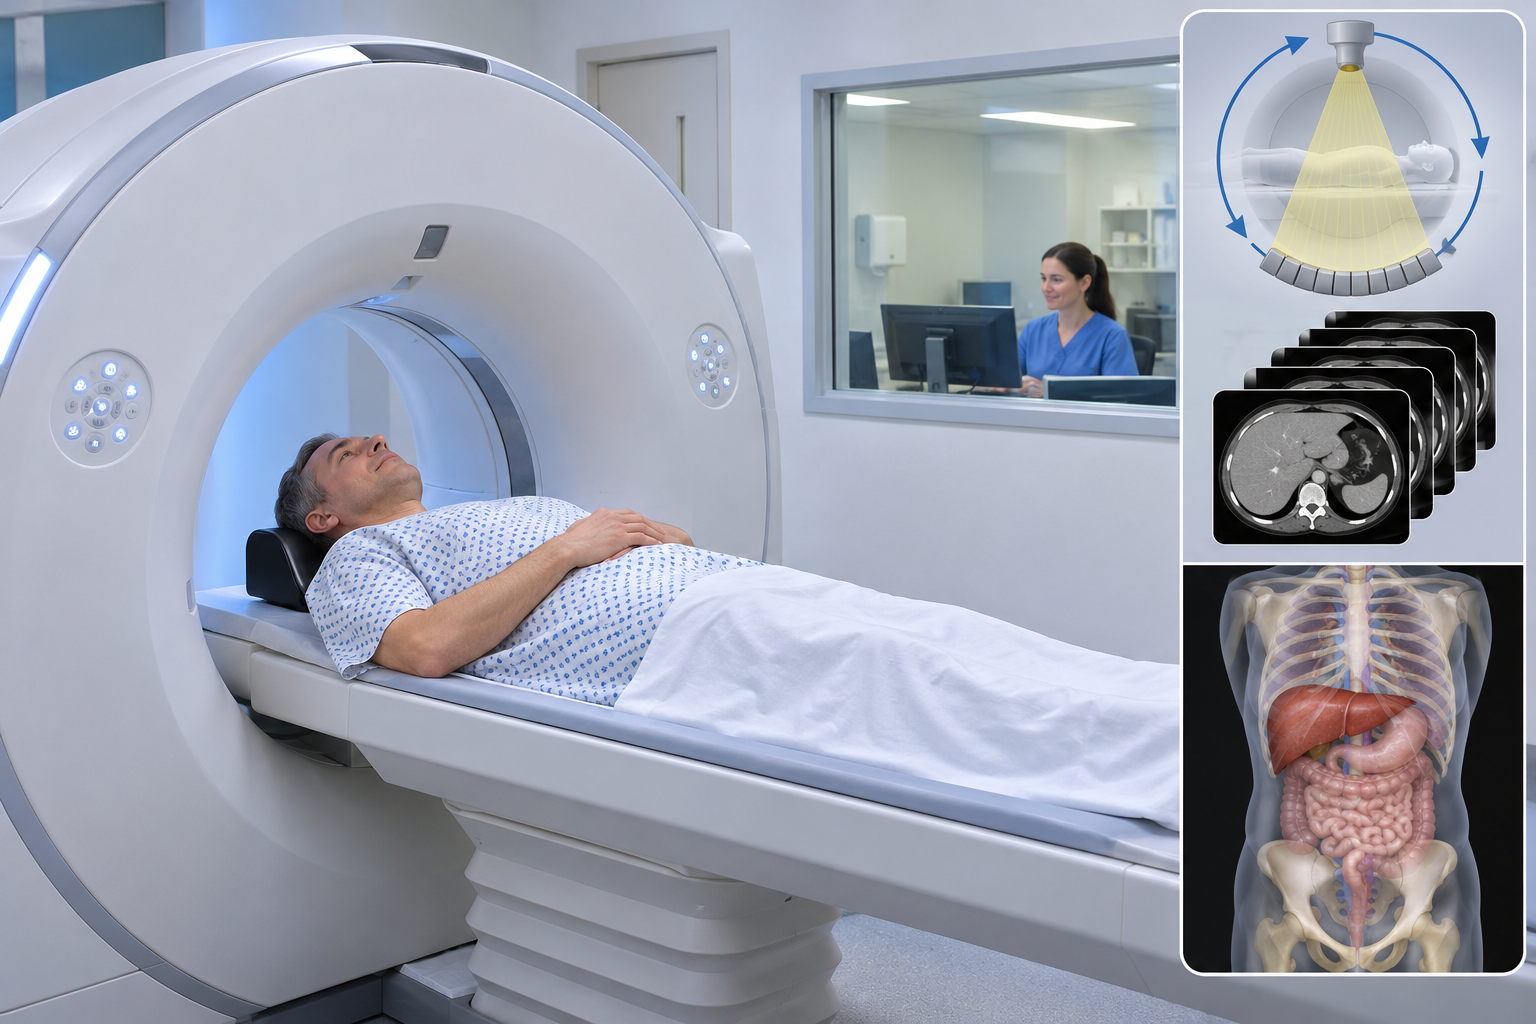
\includegraphics[width=\textwidth,keepaspectratio]{modalities/infographics/computed_tomography_realistic.png}
\end{center}
\begin{center}\footnotesize CT measures X-ray attenuation from many angles and reconstructs cross-sectional images; protocol and contrast phase shape the findings. AI-generated illustration; CT panels are not patient studies.\end{center}

\section{Overview}
Computed tomography (CT) is a cross-sectional imaging technique that uses X-rays and computational reconstruction to visualize internal anatomical structures. CT is particularly valuable for detecting tumors, hemorrhage, fractures, infections, vascular abnormalities, and traumatic injuries.

This catalogue focuses on diseases and conditions for which CT has established clinical diagnostic utility. It includes noncontrast CT, contrast-enhanced CT, high-resolution CT (HRCT), CT angiography (CTA), CT urography, and other specialized CT protocols. It excludes PET-CT and purely interventional applications.

The 312 entries form a preliminary clinical catalogue of diseases, anatomical abnormalities, and radiological findings. Some entries overlap, and not all warrant CT as a first-line investigation. Individual guideline validation is required before using these entries as diagnostic ground truth.

\section{Where CT is used}
The following numbered entries present common diagnostic applications by anatomical system. Findings are examples and should be interpreted with the clinical presentation, acquisition protocol, contrast phase, and reconstruction settings.

\subsection{Brain and intracranial structures}
\begin{enumerate}[leftmargin=*,itemsep=0.45em,topsep=0.4em]
\item \textbf{Acute ischemic stroke.} Useful imaging findings include: Early noncontrast CT may be normal; subtle loss of gray-white differentiation or hypoattenuation may develop.
\item \textbf{Arachnoid cyst.} Useful imaging findings include: Extra-axial fluid-density collection.
\item \textbf{Astrocytoma.} Useful imaging findings include: Intra-axial mass with variable enhancement.
\item \textbf{Brain metastases.} Useful imaging findings include: Enhancing lesions with surrounding edema.
\item \textbf{Cerebral abscess.} Useful imaging findings include: Ring-enhancing lesion with surrounding edema.
\item \textbf{Cerebral atrophy.} Useful imaging findings include: Enlarged sulci and ventricles.
\item \textbf{Cerebral contusion.} Useful imaging findings include: Hemorrhagic parenchymal lesions.
\item \textbf{Cerebral edema.} Useful imaging findings include: Reduced attenuation, sulcal effacement.
\item \textbf{Cerebral herniation.} Useful imaging findings include: Displacement of intracranial structures.
\item \textbf{Cerebral venous sinus thrombosis.} Useful imaging findings include: Venous filling defect on CT venography.
\item \textbf{Craniopharyngioma.} Useful imaging findings include: Cystic or solid suprasellar mass, often calcified.
\item \textbf{Epidural hematoma.} Useful imaging findings include: Biconvex extra-axial collection.
\item \textbf{Glioblastoma.} Useful imaging findings include: Irregular enhancing mass with central necrosis.
\item \textbf{Hydrocephalus.} Useful imaging findings include: Ventricular enlargement.
\item \textbf{Intracerebral hemorrhage.} Useful imaging findings include: Hyperdense intraparenchymal blood.
\item \textbf{Intracranial tuberculoma.} Useful imaging findings include: Nodular or ring-enhancing lesions.
\item \textbf{Intraventricular hemorrhage.} Useful imaging findings include: Hyperdense blood within ventricles.
\item \textbf{Meningioma.} Useful imaging findings include: Enhancing extra-axial mass.
\item \textbf{Neurocysticercosis.} Useful imaging findings include: Cystic lesions or intracranial calcifications.
\item \textbf{Oligodendroglioma.} Useful imaging findings include: Intra-axial mass with possible calcifications.
\item \textbf{Pituitary macroadenoma.} Useful imaging findings include: Enlarged sellar or suprasellar mass.
\item \textbf{Pneumocephalus.} Useful imaging findings include: Intracranial air.
\item \textbf{Subarachnoid hemorrhage.} Useful imaging findings include: Hyperdensity within cerebral sulci and cisterns.
\item \textbf{Subdural hematoma.} Useful imaging findings include: Crescent-shaped extra-axial collection.
\end{enumerate}

\subsection{Head, neck and facial structures}
\begin{enumerate}[leftmargin=*,itemsep=0.45em,topsep=0.4em]
\item \textbf{Acute sinusitis.} Useful imaging findings include: Mucosal thickening or fluid may be seen but is nonspecific; CT is not indicated for uncomplicated disease.
\item \textbf{Branchial cleft cyst.} Useful imaging findings include: Lateral cervical cystic lesion.
\item \textbf{Cervical lymphadenopathy.} Useful imaging findings include: Enlarged or necrotic cervical lymph nodes.
\item \textbf{Cholesteatoma.} Useful imaging findings include: Middle-ear soft tissue with bony erosion.
\item \textbf{Chronic sinusitis.} Useful imaging findings include: Mucosal thickening, bony remodeling.
\item \textbf{Invasive fungal sinusitis.} Useful imaging findings include: Extrasinus infiltration, possible bone destruction.
\item \textbf{Laryngeal carcinoma.} Useful imaging findings include: Laryngeal mass with possible cartilage invasion.
\item \textbf{Ludwig angina.} Useful imaging findings include: Floor-of-mouth inflammatory changes.
\item \textbf{Mastoiditis.} Useful imaging findings include: Mastoid opacification, possible septal erosion.
\item \textbf{Nasal polyposis.} Useful imaging findings include: Polypoid sinonasal soft tissue.
\item \textbf{Nasopharyngeal carcinoma.} Useful imaging findings include: Nasopharyngeal soft-tissue mass.
\item \textbf{Orbital abscess.} Useful imaging findings include: Rim-enhancing orbital collection.
\item \textbf{Orbital cellulitis.} Useful imaging findings include: Orbital fat stranding.
\item \textbf{Orbital fracture.} Useful imaging findings include: Discontinuity of orbital walls.
\item \textbf{Otosclerosis.} Useful imaging findings include: Abnormal otic capsule mineralization.
\item \textbf{Parotid tumor.} Useful imaging findings include: Focal parotid mass.
\item \textbf{Peritonsillar abscess.} Useful imaging findings include: Peritonsillar fluid collection.
\item \textbf{Retropharyngeal abscess.} Useful imaging findings include: Rim-enhancing retropharyngeal collection.
\item \textbf{Sialolithiasis.} Useful imaging findings include: Calcified salivary duct stone.
\item \textbf{Sinus mucocele.} Useful imaging findings include: Expansile opacified sinus.
\item \textbf{Thyroglossal duct cyst.} Useful imaging findings include: Midline cervical cystic lesion.
\item \textbf{Thyroid eye disease.} Useful imaging findings include: Extraocular muscle enlargement.
\end{enumerate}

CT findings of mastoid opacification alone are not specific for acute mastoiditis; bony erosion and clinical evidence of complication increase concern.

\subsection{Pulmonary and thoracic diseases}
\begin{enumerate}[leftmargin=*,itemsep=0.45em,topsep=0.4em]
\item \textbf{Allergic bronchopulmonary aspergillosis.} Useful imaging findings include: Central bronchiectasis and mucus plugging.
\item \textbf{ARDS.} Useful imaging findings include: Bilateral ground-glass opacities and consolidation.
\item \textbf{Asbestosis.} Useful imaging findings include: Subpleural fibrosis, pleural plaques.
\item \textbf{Atelectasis.} Useful imaging findings include: Pulmonary volume loss.
\item \textbf{Bronchiectasis.} Useful imaging findings include: Bronchial dilatation, signet-ring sign.
\item \textbf{Diaphragmatic hernia.} Useful imaging findings include: Abdominal contents within the thorax.
\item \textbf{Empyema.} Useful imaging findings include: Loculated pleural fluid, split-pleura sign.
\item \textbf{Hemothorax.} Useful imaging findings include: High-attenuation pleural fluid.
\item \textbf{Hypersensitivity pneumonitis.} Useful imaging findings include: Mosaic attenuation, centrilobular nodules.
\item \textbf{Idiopathic pulmonary fibrosis.} Useful imaging findings include: Subpleural basal fibrosis and honeycombing.
\item \textbf{Lung abscess.} Useful imaging findings include: Cavitary lesion with air-fluid level.
\item \textbf{Lung carcinoma.} Useful imaging findings include: Pulmonary nodule or mass.
\item \textbf{Lymphangioleiomyomatosis.} Useful imaging findings include: Multiple thin-walled pulmonary cysts.
\item \textbf{Lymphangitic carcinomatosis.} Useful imaging findings include: Nodular interlobular septal thickening.
\item \textbf{Nonspecific interstitial pneumonia.} Useful imaging findings include: Ground-glass opacities and fine reticulation.
\item \textbf{Organizing pneumonia.} Useful imaging findings include: Peripheral or peribronchovascular consolidation.
\item \textbf{Pleural effusion.} Useful imaging findings include: Pleural fluid collection.
\item \textbf{Pleural mesothelioma.} Useful imaging findings include: Nodular pleural thickening.
\item \textbf{Pneumonia.} Useful imaging findings include: Consolidation, ground-glass opacities.
\item \textbf{Pneumothorax.} Useful imaging findings include: Pleural air.
\item \textbf{Pulmonary alveolar proteinosis.} Useful imaging findings include: Crazy-paving pattern.
\item \textbf{Pulmonary aspergilloma.} Useful imaging findings include: Intracavitary fungal mass.
\item \textbf{Pulmonary edema.} Useful imaging findings include: Septal thickening, ground-glass opacities.
\item \textbf{Pulmonary embolism.} Useful imaging findings include: Pulmonary arterial filling defect.
\item \textbf{Pulmonary emphysema.} Useful imaging findings include: Low-attenuation lung regions.
\item \textbf{Pulmonary fibrosis.} Useful imaging findings include: Reticulation, architectural distortion.
\item \textbf{Pulmonary hamartoma.} Useful imaging findings include: Fat-containing nodule, possible popcorn calcification.
\item \textbf{Pulmonary infarction.} Useful imaging findings include: Peripheral wedge-shaped opacity.
\item \textbf{Pulmonary Langerhans cell histiocytosis.} Useful imaging findings include: Upper-lobe nodules and irregular cysts.
\item \textbf{Pulmonary metastases.} Useful imaging findings include: Single or multiple pulmonary nodules.
\item \textbf{Pulmonary sarcoidosis.} Useful imaging findings include: Perilymphatic nodules, hilar lymphadenopathy.
\item \textbf{Pulmonary sequestration.} Useful imaging findings include: Abnormal lung tissue with systemic arterial supply.
\item \textbf{Pulmonary tuberculosis.} Useful imaging findings include: Cavitation, tree-in-bud nodules.
\item \textbf{Silicosis.} Useful imaging findings include: Upper-lobe nodules, possible eggshell calcification.
\item \textbf{Tracheomalacia.} Useful imaging findings include: Expiratory tracheal collapse.
\end{enumerate}

For suspected pulmonary fibrosis, high-resolution CT (HRCT) is the relevant protocol; these patterns are not specific to a single cause.

\subsection{Heart and mediastinum}
\begin{enumerate}[leftmargin=*,itemsep=0.45em,topsep=0.4em]
\item \textbf{Anomalous coronary artery.} Useful imaging findings include: Abnormal coronary origin or course.
\item \textbf{Bronchogenic cyst.} Useful imaging findings include: Mediastinal cystic lesion.
\item \textbf{Constrictive pericarditis.} Useful imaging findings include: Pericardial thickening or calcification.
\item \textbf{Coronary artery aneurysm.} Useful imaging findings include: Focal coronary arterial dilatation.
\item \textbf{Coronary artery calcification.} Useful imaging findings include: Calcified coronary atherosclerotic plaques.
\item \textbf{Coronary artery disease.} Useful imaging findings include: Coronary plaque and luminal stenosis.
\item \textbf{Fibrosing mediastinitis.} Useful imaging findings include: Infiltrative mediastinal fibrosis.
\item \textbf{Left atrial appendage thrombus.} Useful imaging findings include: Persistent intracavitary filling defect.
\item \textbf{Left ventricular aneurysm.} Useful imaging findings include: Ventricular outpouching.
\item \textbf{Mediastinal lymphoma.} Useful imaging findings include: Mediastinal soft-tissue masses or lymphadenopathy.
\item \textbf{Mediastinal teratoma.} Useful imaging findings include: Mixed fat, fluid, and calcified components.
\item \textbf{Mediastinitis.} Useful imaging findings include: Mediastinal inflammatory changes.
\item \textbf{Myocardial bridging.} Useful imaging findings include: Intramyocardial coronary artery segment.
\item \textbf{Pericardial cyst.} Useful imaging findings include: Well-defined fluid-density lesion.
\item \textbf{Pericardial effusion.} Useful imaging findings include: Pericardial fluid.
\item \textbf{Pneumomediastinum.} Useful imaging findings include: Extraluminal mediastinal air.
\item \textbf{Thymic hyperplasia.} Useful imaging findings include: Enlarged thymic tissue.
\item \textbf{Thymoma.} Useful imaging findings include: Anterior mediastinal mass.
\end{enumerate}

\subsection{Liver}
\begin{enumerate}[leftmargin=*,itemsep=0.45em,topsep=0.4em]
\item \textbf{Budd--Chiari syndrome.} Useful imaging findings include: Hepatic venous obstruction and heterogeneous enhancement.
\item \textbf{Congestive hepatopathy.} Useful imaging findings include: Heterogeneous enhancement and dilated hepatic veins.
\item \textbf{Focal nodular hyperplasia.} Useful imaging findings include: Arterial hyperenhancement, possible central scar.
\item \textbf{Hepatic adenoma.} Useful imaging findings include: Hypervascular mass with variable fat or hemorrhage.
\item \textbf{Hepatic hemangioma.} Useful imaging findings include: Peripheral nodular enhancement with progressive fill-in.
\item \textbf{Hepatic hematoma.} Useful imaging findings include: Blood collection within or adjacent to the liver.
\item \textbf{Hepatic infarction.} Useful imaging findings include: Peripheral wedge-shaped hypoenhancement.
\item \textbf{Hepatic metastases.} Useful imaging findings include: Focal lesions with variable enhancement.
\item \textbf{Hepatic steatosis.} Useful imaging findings include: Reduced hepatic attenuation.
\item \textbf{Hepatocellular carcinoma.} Useful imaging findings include: Arterial hyperenhancement and subsequent washout.
\item \textbf{Hepatomegaly.} Useful imaging findings include: Increased liver dimensions.
\item \textbf{Hydatid disease.} Useful imaging findings include: Daughter cysts and possible wall calcification.
\item \textbf{Intrahepatic cholangiocarcinoma.} Useful imaging findings include: Mass with progressive delayed enhancement.
\item \textbf{Liver abscess.} Useful imaging findings include: Rim-enhancing fluid collection.
\item \textbf{Liver cirrhosis.} Useful imaging findings include: Nodular contour and altered hepatic morphology.
\item \textbf{Polycystic liver disease.} Useful imaging findings include: Multiple hepatic cysts.
\item \textbf{Portal hypertension.} Useful imaging findings include: Portosystemic collateral vessels, splenomegaly.
\item \textbf{Simple hepatic cyst.} Useful imaging findings include: Nonenhancing fluid-density lesion.
\end{enumerate}

\subsection{Gallbladder and biliary system}
\begin{enumerate}[leftmargin=*,itemsep=0.45em,topsep=0.4em]
\item \textbf{Acute cholecystitis.} Useful imaging findings include: Gallbladder wall thickening and surrounding inflammation; ultrasound is generally first-line.
\item \textbf{Biliary obstruction.} Useful imaging findings include: Bile duct dilatation.
\item \textbf{Cholangiocarcinoma.} Useful imaging findings include: Biliary mass or irregular ductal narrowing.
\item \textbf{Choledochal cyst.} Useful imaging findings include: Cystic biliary dilatation.
\item \textbf{Choledocholithiasis.} Useful imaging findings include: Visible common bile duct calculus.
\item \textbf{Cholelithiasis.} Useful imaging findings include: Some calcified or otherwise conspicuous stones; CT may miss noncalcified stones, and ultrasound is generally first-line.
\item \textbf{Emphysematous cholecystitis.} Useful imaging findings include: Gas within the gallbladder wall or lumen.
\item \textbf{Gallbladder carcinoma.} Useful imaging findings include: Irregular enhancing mass.
\item \textbf{Gallbladder perforation.} Useful imaging findings include: Focal wall defect and adjacent fluid.
\item \textbf{Gangrenous cholecystitis.} Useful imaging findings include: Irregular or absent mural enhancement.
\item \textbf{Porcelain gallbladder.} Useful imaging findings include: Gallbladder wall calcification.
\end{enumerate}

Ultrasound is generally preferred for the initial assessment of suspected gallstones and uncomplicated acute cholecystitis.

\subsection{Pancreas}
\begin{enumerate}[leftmargin=*,itemsep=0.45em,topsep=0.4em]
\item \textbf{Acute pancreatitis.} Useful imaging findings include: Pancreatic enlargement and surrounding inflammation.
\item \textbf{Autoimmune pancreatitis.} Useful imaging findings include: Diffuse sausage-shaped pancreatic enlargement.
\item \textbf{Chronic pancreatitis.} Useful imaging findings include: Calcifications, ductal dilatation, atrophy.
\item \textbf{Intraductal papillary mucinous neoplasm.} Useful imaging findings include: Pancreatic duct dilatation or communicating cysts.
\item \textbf{Mucinous cystic neoplasm.} Useful imaging findings include: Cystic lesion with septations.
\item \textbf{Necrotizing pancreatitis.} Useful imaging findings include: Nonenhancing pancreatic or peripancreatic tissue.
\item \textbf{Pancreatic adenocarcinoma.} Useful imaging findings include: Hypoenhancing pancreatic mass.
\item \textbf{Pancreatic duct obstruction.} Useful imaging findings include: Upstream pancreatic duct dilatation.
\item \textbf{Pancreatic neuroendocrine tumor.} Useful imaging findings include: Typically hypervascular pancreatic lesion.
\item \textbf{Pancreatic pseudocyst.} Useful imaging findings include: Encapsulated homogeneous fluid collection.
\item \textbf{Serous cystadenoma.} Useful imaging findings include: Multicystic lesion, possible central scar.
\item \textbf{Solid pseudopapillary neoplasm.} Useful imaging findings include: Encapsulated solid-cystic mass.
\item \textbf{Walled-off pancreatic necrosis.} Useful imaging findings include: Encapsulated collection containing necrotic material.
\end{enumerate}

\subsection{Spleen}
\begin{enumerate}[leftmargin=*,itemsep=0.45em,topsep=0.4em]
\item \textbf{Splenic abscess.} Useful imaging findings include: Low-attenuation lesion with possible rim enhancement.
\item \textbf{Splenic cyst.} Useful imaging findings include: Fluid-density lesion.
\item \textbf{Splenic hemangioma.} Useful imaging findings include: Vascular lesion with variable enhancement.
\item \textbf{Splenic hematoma.} Useful imaging findings include: Intraparenchymal or subcapsular blood collection.
\item \textbf{Splenic infarction.} Useful imaging findings include: Peripheral wedge-shaped hypoattenuation.
\item \textbf{Splenic lymphoma.} Useful imaging findings include: Splenomegaly or focal lesions.
\item \textbf{Splenic rupture.} Useful imaging findings include: Parenchymal disruption and hemorrhage.
\item \textbf{Splenic torsion.} Useful imaging findings include: Twisted vascular pedicle and impaired enhancement.
\item \textbf{Splenomegaly.} Useful imaging findings include: Enlarged spleen.
\item \textbf{Wandering spleen.} Useful imaging findings include: Abnormal splenic location.
\end{enumerate}

\subsection{Gastrointestinal system}
\begin{enumerate}[leftmargin=*,itemsep=0.45em,topsep=0.4em]
\item \textbf{Abdominal hernia.} Useful imaging findings include: Protrusion through an abdominal wall defect.
\item \textbf{Acute appendicitis.} Useful imaging findings include: Enlarged appendix with surrounding inflammation.
\item \textbf{Appendiceal abscess.} Useful imaging findings include: Localized rim-enhancing collection.
\item \textbf{Cecal volvulus.} Useful imaging findings include: Displaced dilated cecum with mesenteric twisting.
\item \textbf{Colorectal carcinoma.} Useful imaging findings include: Focal irregular bowel wall thickening.
\item \textbf{Crohn disease.} Useful imaging findings include: Bowel wall thickening, hyperenhancement, comb sign.
\item \textbf{Diverticulitis.} Useful imaging findings include: Inflamed diverticula and pericolic fat stranding.
\item \textbf{Epiploic appendagitis.} Useful imaging findings include: Oval fat-density lesion with hyperattenuating rim.
\item \textbf{Esophageal carcinoma.} Useful imaging findings include: Esophageal wall thickening or mass.
\item \textbf{Gastric carcinoma.} Useful imaging findings include: Irregular gastric wall thickening or mass.
\item \textbf{Gastric volvulus.} Useful imaging findings include: Abnormal gastric rotation.
\item \textbf{Gastrointestinal perforation.} Useful imaging findings include: Extraluminal gas.
\item \textbf{Gastrointestinal stromal tumor.} Useful imaging findings include: Exophytic enhancing gastrointestinal mass.
\item \textbf{Infectious colitis.} Useful imaging findings include: Colonic wall thickening and mucosal enhancement.
\item \textbf{Internal hernia.} Useful imaging findings include: Abnormally positioned bowel loops and mesenteric vessels.
\item \textbf{Intestinal malrotation.} Useful imaging findings include: Abnormal bowel and mesenteric vascular arrangement.
\item \textbf{Intussusception.} Useful imaging findings include: Bowel-within-bowel configuration.
\item \textbf{Ischemic colitis.} Useful imaging findings include: Segmental wall thickening and altered enhancement.
\item \textbf{Large bowel obstruction.} Useful imaging findings include: Proximal colonic dilatation.
\item \textbf{Meckel diverticulitis.} Useful imaging findings include: Inflamed blind-ending bowel structure.
\item \textbf{Mesenteric ischemia.} Useful imaging findings include: Abnormal bowel enhancement, vascular obstruction.
\item \textbf{Omental infarction.} Useful imaging findings include: Focal inflammatory fatty lesion.
\item \textbf{Paralytic ileus.} Useful imaging findings include: Diffuse bowel dilatation without mechanical obstruction.
\item \textbf{Pneumatosis intestinalis.} Useful imaging findings include: Gas within the bowel wall.
\item \textbf{Portal venous gas.} Useful imaging findings include: Peripheral branching hepatic gas.
\item \textbf{Pseudomembranous colitis.} Useful imaging findings include: Marked colonic wall thickening.
\item \textbf{Sigmoid volvulus.} Useful imaging findings include: Twisted mesentery and dilated sigmoid colon.
\item \textbf{Small bowel lymphoma.} Useful imaging findings include: Bowel wall thickening, sometimes aneurysmal dilatation.
\item \textbf{Small bowel obstruction.} Useful imaging findings include: Dilated bowel loops with transition point.
\item \textbf{Stercoral colitis.} Useful imaging findings include: Fecal impaction with surrounding inflammation.
\item \textbf{Superior mesenteric artery syndrome.} Useful imaging findings include: Duodenal compression between the aorta and SMA.
\item \textbf{Toxic megacolon.} Useful imaging findings include: Marked colonic dilatation.
\item \textbf{Ulcerative colitis.} Useful imaging findings include: Continuous colonic wall thickening.
\end{enumerate}

\subsection{Kidneys and urinary tract}
\begin{enumerate}[leftmargin=*,itemsep=0.45em,topsep=0.4em]
\item \textbf{Acute pyelonephritis.} Useful imaging findings include: Striated nephrogram or wedge-shaped hypoenhancement in selected complicated cases; routine imaging is unnecessary for uncomplicated first presentations.
\item \textbf{Bladder carcinoma.} Useful imaging findings include: Focal bladder wall mass.
\item \textbf{Bladder stones.} Useful imaging findings include: Intraluminal calculi.
\item \textbf{Complex renal cyst.} Useful imaging findings include: Septations, thickened walls, or enhancing components.
\item \textbf{Emphysematous cystitis.} Useful imaging findings include: Gas within the bladder wall.
\item \textbf{Emphysematous pyelonephritis.} Useful imaging findings include: Gas within renal tissue or surrounding spaces.
\item \textbf{Horseshoe kidney.} Useful imaging findings include: Fusion of renal poles.
\item \textbf{Hydronephrosis.} Useful imaging findings include: Dilated renal collecting system.
\item \textbf{Hydroureter.} Useful imaging findings include: Dilated ureter.
\item \textbf{Nephrolithiasis.} Useful imaging findings include: Renal calculi.
\item \textbf{Perinephric abscess.} Useful imaging findings include: Fluid collection surrounding the kidney.
\item \textbf{Polycystic kidney disease.} Useful imaging findings include: Multiple bilateral renal cysts.
\item \textbf{Renal abscess.} Useful imaging findings include: Rim-enhancing renal collection.
\item \textbf{Renal angiomyolipoma.} Useful imaging findings include: Renal mass containing macroscopic fat.
\item \textbf{Renal atrophy.} Useful imaging findings include: Reduced renal size.
\item \textbf{Renal cell carcinoma.} Useful imaging findings include: Enhancing renal mass.
\item \textbf{Renal infarction.} Useful imaging findings include: Wedge-shaped nonenhancing renal region.
\item \textbf{Renal oncocytoma.} Useful imaging findings include: Enhancing solid renal mass; CT cannot reliably distinguish oncocytoma from renal malignancy.
\item \textbf{Renal papillary necrosis.} Useful imaging findings include: Papillary abnormalities on excretory-phase imaging.
\item \textbf{Renal tuberculosis.} Useful imaging findings include: Calyceal deformity and calcification.
\item \textbf{Retroperitoneal fibrosis.} Useful imaging findings include: Periaortic soft tissue encasing retroperitoneal structures.
\item \textbf{Simple renal cyst.} Useful imaging findings include: Nonenhancing fluid-density lesion.
\item \textbf{Staghorn calculus.} Useful imaging findings include: Branching renal collecting system calculus.
\item \textbf{Ureterolithiasis.} Useful imaging findings include: Ureteral calculi.
\item \textbf{Ureteropelvic junction obstruction.} Useful imaging findings include: Collecting system dilatation with junctional narrowing.
\item \textbf{Urinary bladder rupture.} Useful imaging findings include: Extraluminal contrast on CT cystography.
\item \textbf{Urothelial carcinoma.} Useful imaging findings include: Enhancing lesion or urinary tract filling defect.
\item \textbf{Xanthogranulomatous pyelonephritis.} Useful imaging findings include: Enlarged kidney with bear-paw appearance.
\end{enumerate}

\subsection{Adrenal glands}
\begin{enumerate}[leftmargin=*,itemsep=0.45em,topsep=0.4em]
\item \textbf{Adrenal adenoma.} Useful imaging findings include: Low unenhanced attenuation or characteristic contrast washout.
\item \textbf{Adrenal carcinoma.} Useful imaging findings include: Large heterogeneous adrenal mass.
\item \textbf{Adrenal cyst.} Useful imaging findings include: Fluid-density adrenal lesion.
\item \textbf{Adrenal hemorrhage.} Useful imaging findings include: Hyperattenuating adrenal enlargement.
\item \textbf{Adrenal hyperplasia.} Useful imaging findings include: Diffuse or nodular adrenal enlargement.
\item \textbf{Adrenal metastases.} Useful imaging findings include: Adrenal masses with variable enhancement.
\item \textbf{Adrenal myelolipoma.} Useful imaging findings include: Macroscopic fat-containing adrenal mass.
\item \textbf{Adrenal tuberculosis.} Useful imaging findings include: Adrenal enlargement or calcification.
\item \textbf{Pheochromocytoma.} Useful imaging findings include: Adrenal mass with variable enhancement.
\end{enumerate}

\subsection{Female reproductive system and pelvis}
\begin{enumerate}[leftmargin=*,itemsep=0.45em,topsep=0.4em]
\item \textbf{Cervical carcinoma.} Useful imaging findings include: Cervical mass and possible adjacent invasion.
\item \textbf{Endometrial carcinoma.} Useful imaging findings include: Endometrial mass or uterine cavity abnormality.
\item \textbf{Hydrosalpinx.} Useful imaging findings include: Dilated fluid-filled fallopian tube.
\item \textbf{Ovarian carcinoma.} Useful imaging findings include: Complex adnexal mass, possible peritoneal metastases.
\item \textbf{Ovarian cyst.} Useful imaging findings include: Fluid-density adnexal lesion.
\item \textbf{Ovarian dermoid cyst.} Useful imaging findings include: Fat-containing adnexal lesion.
\item \textbf{Ovarian torsion.} Useful imaging findings include: Enlarged ovary or twisted pedicle may be visible; ultrasound is generally first-line and CT does not exclude torsion.
\item \textbf{Ovarian vein thrombosis.} Useful imaging findings include: Venous filling defect.
\item \textbf{Pelvic congestion.} Useful imaging findings include: Dilated pelvic venous structures.
\item \textbf{Pelvic hematoma.} Useful imaging findings include: Hyperattenuating pelvic collection.
\item \textbf{Pelvic inflammatory disease.} Useful imaging findings include: Pelvic inflammatory changes.
\item \textbf{Tubo-ovarian abscess.} Useful imaging findings include: Complex rim-enhancing adnexal collection.
\item \textbf{Uterine fibroids.} Useful imaging findings include: Uterine masses with variable enhancement or calcification; ultrasound or MRI is preferred for primary characterization.
\end{enumerate}

Ultrasound and MRI are generally preferred for primary characterization of gynecological abnormalities. CT is valuable in emergencies, complications, and cancer staging.

\subsection{Blood vessels and vascular diseases}
\textbf{Imaging protocols:} CT angiography (CTA), CT venography (CTV).

\begin{enumerate}[leftmargin=*,itemsep=0.45em,topsep=0.4em]
\item \textbf{Abdominal aortic aneurysm.} Useful imaging findings include: Aortic dilatation.
\item \textbf{Aortic coarctation.} Useful imaging findings include: Focal aortic narrowing.
\item \textbf{Aortic dissection.} Useful imaging findings include: Intimal flap separating true and false lumens.
\item \textbf{Aortic intramural hematoma.} Useful imaging findings include: Crescent-shaped aortic wall thickening.
\item \textbf{Arterial pseudoaneurysm.} Useful imaging findings include: Contrast-filled extravascular sac.
\item \textbf{Arteriovenous fistula.} Useful imaging findings include: Early venous opacification.
\item \textbf{Carotid artery dissection.} Useful imaging findings include: Tapered narrowing, mural hematoma, or intimal flap.
\item \textbf{Carotid artery stenosis.} Useful imaging findings include: Carotid luminal narrowing.
\item \textbf{Cerebral arterial occlusion.} Useful imaging findings include: Interrupted arterial opacification.
\item \textbf{Cerebral arteriovenous malformation.} Useful imaging findings include: Abnormal vascular nidus.
\item \textbf{Cerebral vasospasm.} Useful imaging findings include: Segmental intracranial arterial narrowing.
\item \textbf{Deep vein thrombosis.} Useful imaging findings include: Venous filling defect.
\item \textbf{Endoleak following aneurysm repair.} Useful imaging findings include: Contrast outside the endovascular graft.
\item \textbf{Fibromuscular dysplasia.} Useful imaging findings include: String-of-beads arterial appearance.
\item \textbf{Inferior vena cava thrombosis.} Useful imaging findings include: Intraluminal venous filling defect.
\item \textbf{Intracranial aneurysm.} Useful imaging findings include: Focal arterial outpouching.
\item \textbf{Mesenteric arterial thrombosis.} Useful imaging findings include: Arterial filling defect.
\item \textbf{Mesenteric artery stenosis.} Useful imaging findings include: Mesenteric arterial narrowing.
\item \textbf{Mesenteric venous thrombosis.} Useful imaging findings include: Venous filling defect.
\item \textbf{Penetrating atherosclerotic ulcer.} Useful imaging findings include: Contrast-filled ulcer extending into aortic wall.
\item \textbf{Peripheral arterial disease.} Useful imaging findings include: Peripheral arterial stenosis or occlusion.
\item \textbf{Portal vein thrombosis.} Useful imaging findings include: Portal venous filling defect.
\item \textbf{Renal artery stenosis.} Useful imaging findings include: Renal arterial narrowing.
\item \textbf{Ruptured aortic aneurysm.} Useful imaging findings include: Periaortic or retroperitoneal hemorrhage.
\item \textbf{Thoracic aortic aneurysm.} Useful imaging findings include: Thoracic aortic dilatation.
\item \textbf{Vascular malformation.} Useful imaging findings include: Abnormal vascular channels.
\end{enumerate}

\subsection{Bones and joints}
\begin{enumerate}[leftmargin=*,itemsep=0.45em,topsep=0.4em]
\item \textbf{Bone metastases.} Useful imaging findings include: Lytic, sclerotic, or mixed lesions.
\item \textbf{Chondrosarcoma.} Useful imaging findings include: Chondroid matrix calcification.
\item \textbf{Complex bone fracture.} Useful imaging findings include: Cortical disruption and fracture fragments.
\item \textbf{Ewing sarcoma.} Useful imaging findings include: Destructive bone lesion and soft-tissue component.
\item \textbf{Facial fracture.} Useful imaging findings include: Facial skeletal discontinuity.
\item \textbf{Fibrous dysplasia.} Useful imaging findings include: Ground-glass bone matrix.
\item \textbf{Giant cell tumor.} Useful imaging findings include: Expansile lytic lesion.
\item \textbf{Gout.} Useful imaging findings include: Erosions and urate deposits on dual-energy CT.
\item \textbf{Multiple myeloma.} Useful imaging findings include: Multiple lytic bone lesions.
\item \textbf{Osteoarthritis.} Useful imaging findings include: Osteophytes, joint space narrowing.
\item \textbf{Osteoblastoma.} Useful imaging findings include: Expansile bone-forming lesion.
\item \textbf{Osteochondroma.} Useful imaging findings include: Cortical and medullary continuity with parent bone.
\item \textbf{Osteoid osteoma.} Useful imaging findings include: Small lucent nidus surrounded by sclerosis.
\item \textbf{Osteomyelitis.} Useful imaging findings include: Cortical destruction or sequestrum, particularly in chronic disease; MRI is more sensitive for early marrow infection.
\item \textbf{Osteonecrosis.} Useful imaging findings include: Sclerosis or subchondral collapse in established disease; MRI is more sensitive for early disease.
\item \textbf{Osteosarcoma.} Useful imaging findings include: Destructive bone lesion with mineralized matrix.
\item \textbf{Paget disease.} Useful imaging findings include: Bone expansion and cortical thickening.
\item \textbf{Pelvic fracture.} Useful imaging findings include: Pelvic ring or acetabular disruption.
\item \textbf{Rib fracture.} Useful imaging findings include: Rib cortical discontinuity.
\item \textbf{Skull fracture.} Useful imaging findings include: Cranial bone discontinuity.
\end{enumerate}

\subsection{Spine}
\begin{enumerate}[leftmargin=*,itemsep=0.45em,topsep=0.4em]
\item \textbf{Ankylosing spondylitis.} Useful imaging findings include: Syndesmophytes and sacroiliac fusion.
\item \textbf{Degenerative disc disease.} Useful imaging findings include: Disc space narrowing and vacuum phenomenon.
\item \textbf{Diffuse idiopathic skeletal hyperostosis.} Useful imaging findings include: Flowing ligamentous ossification.
\item \textbf{Disc herniation.} Useful imaging findings include: May show calcified or large disc material; MRI is generally preferred for nerve-root and soft-tissue assessment.
\item \textbf{Neural foraminal stenosis.} Useful imaging findings include: Narrowed neural foramina.
\item \textbf{Ossification of posterior longitudinal ligament.} Useful imaging findings include: Ossified ligament within the spinal canal.
\item \textbf{Sacroiliitis.} Useful imaging findings include: Sacroiliac erosions and sclerosis.
\item \textbf{Spinal metastases.} Useful imaging findings include: Destructive or sclerotic vertebral lesions.
\item \textbf{Spinal stenosis.} Useful imaging findings include: Narrowing of the spinal canal.
\item \textbf{Spinal tuberculosis.} Useful imaging findings include: Vertebral destruction and paravertebral collections.
\item \textbf{Spondylolisthesis.} Useful imaging findings include: Vertebral displacement.
\item \textbf{Spondylolysis.} Useful imaging findings include: Pars interarticularis defect.
\item \textbf{Vertebral burst fracture.} Useful imaging findings include: Vertebral fragmentation with possible retropulsion.
\item \textbf{Vertebral compression fracture.} Useful imaging findings include: Vertebral height loss.
\item \textbf{Vertebral hemangioma.} Useful imaging findings include: Polka-dot or corduroy appearance.
\item \textbf{Vertebral osteomyelitis.} Useful imaging findings include: Endplate erosion and bone destruction.
\end{enumerate}

MRI is generally superior for evaluating the spinal cord, nerve roots, bone marrow, and many soft-tissue abnormalities.

\subsection{Peritoneum, retroperitoneum and soft tissues}
\begin{enumerate}[leftmargin=*,itemsep=0.45em,topsep=0.4em]
\item \textbf{Abdominal abscess.} Useful imaging findings include: Rim-enhancing fluid collection.
\item \textbf{Abdominal lymphadenopathy.} Useful imaging findings include: Enlarged abdominal lymph nodes.
\item \textbf{Ascites.} Useful imaging findings include: Free intraperitoneal fluid.
\item \textbf{Cellulitis.} Useful imaging findings include: Subcutaneous edema and fat stranding.
\item \textbf{Hemoperitoneum.} Useful imaging findings include: High-attenuation intraperitoneal fluid.
\item \textbf{Lipoma.} Useful imaging findings include: Homogeneous fat-density mass.
\item \textbf{Necrotizing fasciitis.} Useful imaging findings include: Fascial thickening, fluid, and possible gas.
\item \textbf{Peritoneal carcinomatosis.} Useful imaging findings include: Peritoneal nodules and omental caking.
\item \textbf{Peritonitis.} Useful imaging findings include: Peritoneal thickening and enhancement.
\item \textbf{Pseudomyxoma peritonei.} Useful imaging findings include: Mucinous collections with visceral scalloping.
\item \textbf{Psoas abscess.} Useful imaging findings include: Rim-enhancing intramuscular collection.
\item \textbf{Retroperitoneal hematoma.} Useful imaging findings include: Retroperitoneal blood collection.
\item \textbf{Retroperitoneal liposarcoma.} Useful imaging findings include: Large fat-containing or heterogeneous mass.
\item \textbf{Retroperitoneal lymphoma.} Useful imaging findings include: Retroperitoneal lymphadenopathy.
\item \textbf{Soft-tissue hematoma.} Useful imaging findings include: Blood collection within soft tissue.
\item \textbf{Soft-tissue sarcoma.} Useful imaging findings include: Heterogeneous soft-tissue mass.
\end{enumerate}

\subsection{Summary}
\begin{center}
\begin{tabular}{@{}p{0.70\textwidth}r@{}}
\toprule
\textbf{Disease category} & \textbf{Entries} \\
\midrule
Anatomical system & Conditions and findings \\
Adrenal glands & 9 \\
Bones and joints & 20 \\
Brain and intracranial structures & 24 \\
Female reproductive system and pelvis & 13 \\
Gallbladder and biliary system & 11 \\
Gastrointestinal system & 33 \\
Head, neck and facial structures & 22 \\
Heart and mediastinum & 18 \\
Kidneys and urinary tract & 28 \\
Liver & 18 \\
Pancreas & 13 \\
Peritoneum, retroperitoneum and soft tissues & 16 \\
Pulmonary and thoracic diseases & 35 \\
Spine & 16 \\
Spleen & 10 \\
Total & 312 \\
Vascular diseases & 26 \\
\bottomrule
\end{tabular}
\end{center}

\subsection{Types of computed tomography}
\begin{longtable}{@{}p{0.38\textwidth}p{0.56\textwidth}@{}}
\toprule
\textbf{CT technique} & \textbf{Primary diagnostic application} \\
\midrule
\endfirsthead
\toprule
\textbf{CT technique} & \textbf{Primary diagnostic application} \\
\midrule
\endhead
Cardiac CT & Coronary arteries and cardiac anatomy \\
Cone-beam CT (CBCT) & Dental and maxillofacial abnormalities \\
Contrast-enhanced CT (CECT) & Tumors, infections, inflammation \\
CT angiography (CTA) & Arterial abnormalities \\
CT colonography & Colorectal polyps and tumors \\
CT cystography & Urinary bladder injuries \\
CT enterography & Small bowel diseases \\
CT myelography & Spinal canal and nerve root assessment \\
CT perfusion (CTP) & Tissue perfusion abnormalities \\
CT urography & Urinary tract abnormalities \\
CT venography (CTV) & Venous thrombosis \\
Dual-energy CT (DECT) & Material differentiation and tissue characterization \\
High-resolution CT (HRCT) & Interstitial lung diseases \\
Low-dose CT (LDCT) & Lung cancer screening and selected other indications \\
Multiphasic CT & Liver, pancreatic, and renal tumor characterization \\
Noncontrast CT (NCCT) & Hemorrhage, fractures, urinary calculi \\
Photon-counting CT & High-resolution imaging and spectral characterization \\
\bottomrule
\end{longtable}

\subsection{Published clinical CT images and datasets}
\begin{longtable}{@{}p{0.40\textwidth}p{0.54\textwidth}@{}}
\toprule
\textbf{Source} & \textbf{Primary utility} \\
\midrule
\endfirsthead
\toprule
\textbf{Source} & \textbf{Primary utility} \\
\midrule
\endhead
ACR Appropriateness Criteria & Clinical indications for imaging \\
DeepLesion & Large-scale CT lesion annotations \\
LIDC-IDRI & Lung nodule CT images and annotations \\
Medical Segmentation Decathlon & Medical image segmentation datasets \\
PubMed Central & Published clinical CT images \\
Radiopaedia & Annotated clinical CT cases \\
The Cancer Imaging Archive (TCIA) & Oncological CT datasets \\
The Radiology Assistant & Diagnostic imaging education \\
TotalSegmentator & Anatomical CT segmentation \\
\bottomrule
\end{longtable}

\subsection{Recommended metadata for a CT imaging dataset}
\begin{longtable}{@{}p{0.45\textwidth}p{0.49\textwidth}@{}}
\toprule
\textbf{Attribute} & \textbf{Example} \\
\midrule
Acquisition protocol & Multiphasic contrast-enhanced CT \\
Anatomical region & Liver \\
Annotation & Bounding box, segmentation mask \\
Contrast phase & Arterial, portal venous, delayed \\
Diagnostic reference standard & Histopathology or validated imaging criteria \\
Disease & Hepatocellular carcinoma \\
Image format & DICOM \\
Image license & CC BY, CC0, or other specified license \\
Image orientation & Axial, coronal, sagittal \\
Imaging modality & Computed tomography \\
Publication reference & DOI or PMID \\
Radiological finding & Arterial hyperenhancement \\
Reconstruction kernel & Soft tissue \\
Slice thickness & 1 mm \\
Tissue attenuation & Hounsfield units (HU) \\
\bottomrule
\end{longtable}

\subsection{Selected clinical guidance}
These guidelines support the protocol and diagnostic limitations noted above:
\begin{itemize}
\item \href{https://acsearch.acr.org/docs/69502/Narrative/}{ACR Appropriateness Criteria: Sinonasal Disease} (imaging is generally unnecessary for uncomplicated acute rhinosinusitis).
\item \href{https://acsearch.acr.org/docs/69489/Narrative}{ACR Appropriateness Criteria: Acute Pyelonephritis} (routine imaging is generally unnecessary in uncomplicated first presentations).
\item \href{https://uroweb.org/guidelines/renal-cell-carcinoma/chapter/diagnostic-evaluation}{European Association of Urology Guidelines: Renal Cell Carcinoma} (CT/MRI do not reliably distinguish oncocytoma from malignant renal masses).
\item \href{https://acsearch.acr.org/docs/3094201/Narrative}{ACR Appropriateness Criteria: Suspected Osteomyelitis, Septic Arthritis, or Soft-Tissue Infection} (modality choice depends on the clinical setting; MRI is important for early marrow disease).
\end{itemize}

For medical imaging research, CT should primarily be treated as a three-dimensional volumetric imaging modality rather than a collection of independent two-dimensional images. Diagnostic information may depend on multiple consecutive slices, reconstruction planes, contrast phases, and window settings.

The 312 entries constitute a preliminary clinical catalogue, including diseases, anatomical abnormalities, and radiological findings. Some overlap, and not all warrant CT as a first-line investigation. Individual guideline validation is required before using them as diagnostic ground truth.

\chapter{Magnetic Resonance Imaging (MRI)}
\label{ch:mri}

% Chapter-opening illustrated modality infographic.
\begin{center}
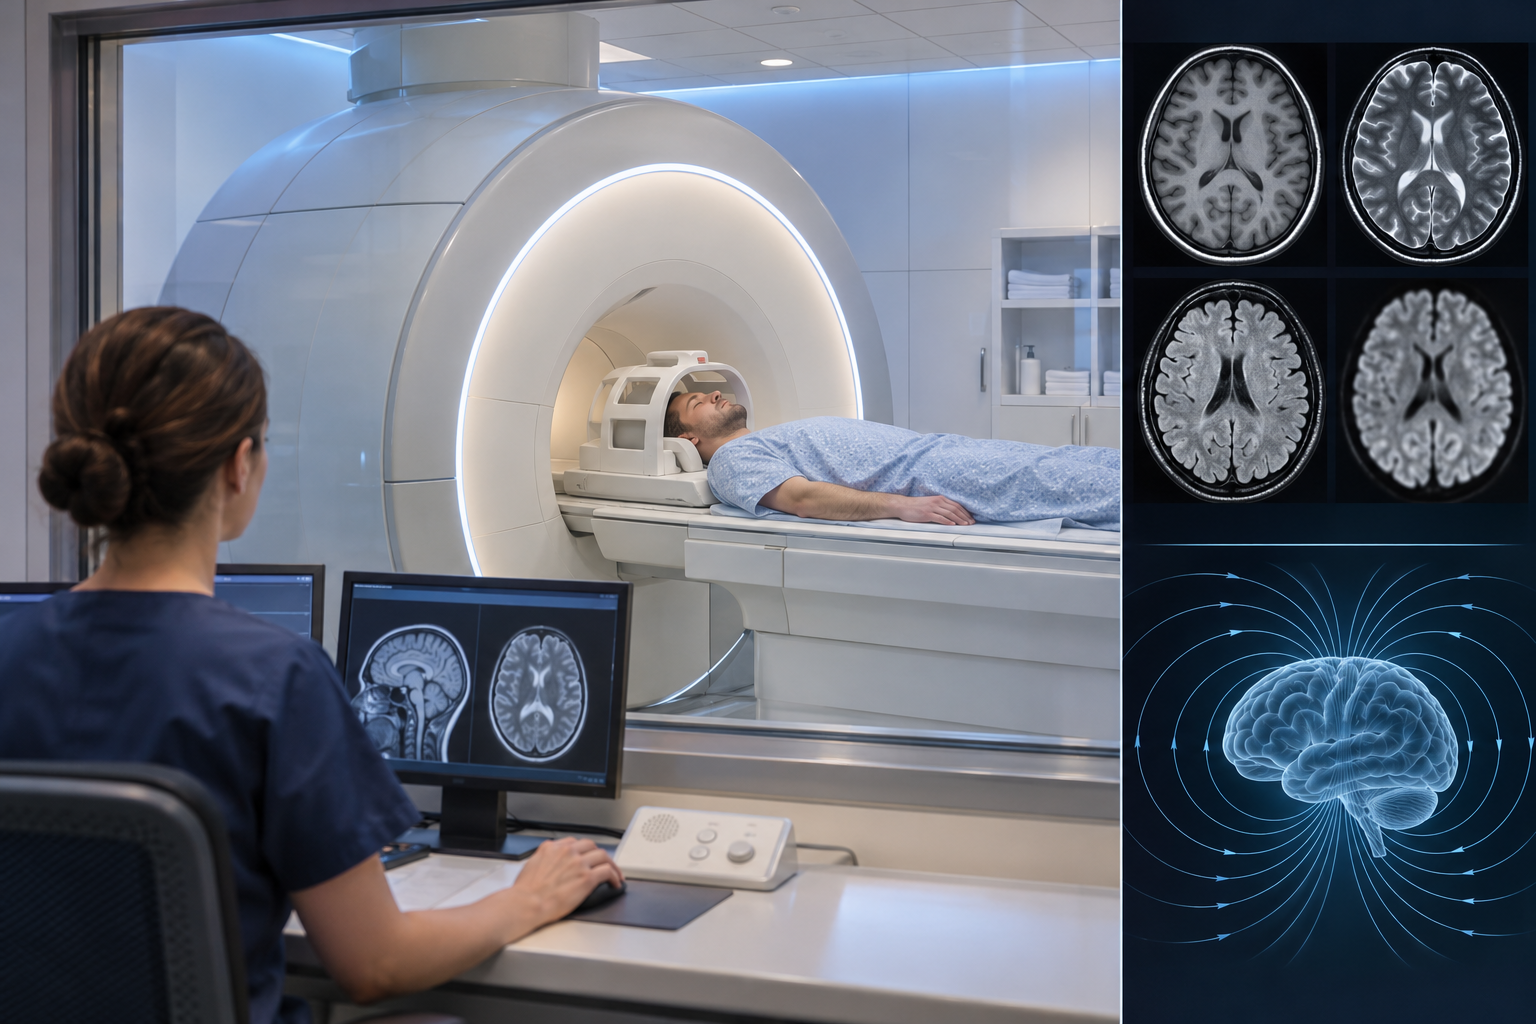
\includegraphics[width=\textwidth,keepaspectratio]{modalities/infographics/mri_realistic.png}
\end{center}
\begin{center}\footnotesize MRI uses magnetic fields and radiofrequency pulses; different sequences emphasize different tissue properties without ionizing radiation. AI-generated illustration; MRI panels are not patient studies.\end{center}

\section{Overview}
Magnetic Resonance Imaging (MRI) is a diagnostic imaging modality that uses strong magnetic fields, radiofrequency pulses, and computational reconstruction to visualize anatomical structures, tissue composition, physiological function, and blood flow.

MRI is particularly valuable for examining the brain, spinal cord, muscles, ligaments, cartilage, bone marrow, cardiovascular system, and internal organs because of its superior soft-tissue contrast.

This catalogue focuses on diseases and conditions for which MRI has established clinical diagnostic utility. It includes functional MRI (fMRI), diffusion-weighted imaging (DWI), magnetic resonance angiography (MRA), magnetic resonance venography (MRV), magnetic resonance cholangiopancreatography (MRCP), and other specialized MRI techniques.

\section{Where MRI is used}
The numbered entries below summarize characteristic MRI findings by anatomical system. Findings depend on the sequence, field strength, acquisition protocol, and clinical context; they are not, by themselves, definitive diagnoses.

\subsection{Brain and neurological disorders}
\begin{enumerate}[leftmargin=*,itemsep=0.45em,topsep=0.4em]
\item \textbf{Acute disseminated encephalomyelitis.} Useful imaging findings include: Multifocal white-matter lesions.
\item \textbf{Acute ischemic stroke.} Useful imaging findings include: Restricted diffusion on DWI.
\item \textbf{Agenesis of the corpus callosum.} Useful imaging findings include: Partial or complete absence of the corpus callosum.
\item \textbf{Alzheimer disease.} Useful imaging findings include: Medial temporal and hippocampal atrophy.
\item \textbf{Arachnoid cyst.} Useful imaging findings include: CSF-equivalent extra-axial lesion.
\item \textbf{CADASIL.} Useful imaging findings include: Anterior temporal and external capsule white-matter lesions.
\item \textbf{Central pontine myelinolysis.} Useful imaging findings include: Central pontine T2 hyperintensity.
\item \textbf{Cerebral contusion.} Useful imaging findings include: Parenchymal edema and hemorrhage.
\item \textbf{Cerebral edema.} Useful imaging findings include: Increased T2/FLAIR signal.
\item \textbf{Cerebral microbleeds.} Useful imaging findings include: Susceptibility artifacts on SWI.
\item \textbf{Cerebral small vessel disease.} Useful imaging findings include: White-matter hyperintensities, lacunes and microbleeds.
\item \textbf{Chiari malformation.} Useful imaging findings include: Cerebellar tonsillar displacement.
\item \textbf{Chronic cerebral infarction.} Useful imaging findings include: Encephalomalacia and gliosis.
\item \textbf{Creutzfeldt--Jakob disease.} Useful imaging findings include: Cortical ribboning and basal ganglia diffusion restriction.
\item \textbf{Dandy--Walker malformation.} Useful imaging findings include: Vermian abnormality and posterior fossa cystic dilatation.
\item \textbf{Diffuse axonal injury.} Useful imaging findings include: Small hemorrhagic or nonhemorrhagic white-matter lesions.
\item \textbf{Epidural hematoma.} Useful imaging findings include: Biconvex extra-axial collection.
\item \textbf{Focal cortical dysplasia.} Useful imaging findings include: Cortical thickening and blurred gray-white matter junction.
\item \textbf{Frontotemporal dementia.} Useful imaging findings include: Frontal and temporal lobe atrophy.
\item \textbf{Huntington disease.} Useful imaging findings include: Caudate nucleus atrophy.
\item \textbf{Hydrocephalus.} Useful imaging findings include: Ventricular enlargement.
\item \textbf{Hypoxic-ischemic brain injury.} Useful imaging findings include: Cortical or deep gray-matter diffusion restriction.
\item \textbf{Intracerebral hemorrhage.} Useful imaging findings include: Stage-dependent signal changes.
\item \textbf{Lissencephaly.} Useful imaging findings include: Abnormally smooth cerebral cortex.
\item \textbf{Mesial temporal sclerosis.} Useful imaging findings include: Hippocampal atrophy and increased T2 signal.
\item \textbf{MOG antibody-associated disease.} Useful imaging findings include: Inflammatory demyelinating lesions.
\item \textbf{Multiple sclerosis.} Useful imaging findings include: Periventricular, juxtacortical or infratentorial demyelinating lesions.
\item \textbf{Multiple system atrophy.} Useful imaging findings include: Pontocerebellar or putaminal abnormalities.
\item \textbf{Neuromyelitis optica spectrum disorder.} Useful imaging findings include: Characteristic optic nerve, brainstem or spinal cord lesions.
\item \textbf{Normal pressure hydrocephalus.} Useful imaging findings include: Ventriculomegaly with characteristic CSF-space distribution.
\item \textbf{Polymicrogyria.} Useful imaging findings include: Excessive small cerebral gyri.
\item \textbf{Posterior reversible encephalopathy syndrome.} Useful imaging findings include: Predominantly posterior vasogenic edema.
\item \textbf{Progressive multifocal leukoencephalopathy.} Useful imaging findings include: Asymmetric white-matter abnormalities.
\item \textbf{Progressive supranuclear palsy.} Useful imaging findings include: Midbrain atrophy, hummingbird sign.
\item \textbf{Schizencephaly.} Useful imaging findings include: Gray matter-lined cerebral cleft.
\item \textbf{Subarachnoid hemorrhage.} Useful imaging findings include: Abnormal sulcal signal on FLAIR.
\item \textbf{Subdural hematoma.} Useful imaging findings include: Crescent-shaped extra-axial collection.
\item \textbf{Vascular dementia.} Useful imaging findings include: Multiple infarcts and white-matter abnormalities.
\item \textbf{Wernicke encephalopathy.} Useful imaging findings include: Abnormal signal in medial thalami and mammillary bodies.
\item \textbf{Wilson disease.} Useful imaging findings include: Basal ganglia signal abnormalities.
\end{enumerate}

For acute intracranial hemorrhage or suspected subarachnoid hemorrhage, noncontrast CT is commonly the initial examination in emergency care. MRI can provide complementary information, and the appropriate test depends on timing and clinical circumstances.

\subsection{Brain tumors}
\begin{enumerate}[leftmargin=*,itemsep=0.45em,topsep=0.4em]
\item \textbf{Astrocytoma.} Useful imaging findings include: Infiltrative T2/FLAIR hyperintense lesion.
\item \textbf{Brain metastases.} Useful imaging findings include: Enhancing lesions with surrounding vasogenic edema.
\item \textbf{Central neurocytoma.} Useful imaging findings include: Intraventricular mass.
\item \textbf{Choroid plexus papilloma.} Useful imaging findings include: Enhancing intraventricular mass.
\item \textbf{Craniopharyngioma.} Useful imaging findings include: Solid-cystic suprasellar mass.
\item \textbf{Dermoid cyst.} Useful imaging findings include: Fat-containing intracranial lesion.
\item \textbf{Dysembryoplastic neuroepithelial tumor.} Useful imaging findings include: Multinodular cortical lesion.
\item \textbf{Ependymoma.} Useful imaging findings include: Ventricular-associated mass.
\item \textbf{Epidermoid cyst.} Useful imaging findings include: Restricted diffusion within a CSF-like lesion.
\item \textbf{Ganglioglioma.} Useful imaging findings include: Cortical solid-cystic lesion.
\item \textbf{Glioblastoma.} Useful imaging findings include: Irregular enhancement, necrosis and surrounding edema.
\item \textbf{Hemangioblastoma.} Useful imaging findings include: Hypervascular mural nodule with associated cyst.
\item \textbf{Medulloblastoma.} Useful imaging findings include: Posterior fossa mass with restricted diffusion.
\item \textbf{Meningioma.} Useful imaging findings include: Enhancing extra-axial mass, possible dural tail.
\item \textbf{Oligodendroglioma.} Useful imaging findings include: Cortical-subcortical infiltrative mass.
\item \textbf{Pilocytic astrocytoma.} Useful imaging findings include: Cystic lesion with enhancing mural nodule.
\item \textbf{Pineal region tumor.} Useful imaging findings include: Pineal region mass.
\item \textbf{Pituitary adenoma.} Useful imaging findings include: Sellar mass with variable enhancement.
\item \textbf{Primary CNS lymphoma.} Useful imaging findings include: Enhancing mass with restricted diffusion.
\item \textbf{Vestibular schwannoma.} Useful imaging findings include: Enhancing internal auditory canal or cerebellopontine angle mass.
\end{enumerate}

\subsection{Central nervous system infections}
\begin{enumerate}[leftmargin=*,itemsep=0.45em,topsep=0.4em]
\item \textbf{Bacterial meningitis.} Useful imaging findings include: Leptomeningeal enhancement.
\item \textbf{Cerebral abscess.} Useful imaging findings include: Ring enhancement with central diffusion restriction.
\item \textbf{Cerebral toxoplasmosis.} Useful imaging findings include: Multiple ring-enhancing lesions.
\item \textbf{Herpes simplex encephalitis.} Useful imaging findings include: Temporal and insular signal abnormalities.
\item \textbf{Intracranial tuberculoma.} Useful imaging findings include: Nodular or ring-enhancing lesions.
\item \textbf{Neurocysticercosis.} Useful imaging findings include: Cystic lesions, sometimes with an identifiable scolex.
\item \textbf{Subdural empyema.} Useful imaging findings include: Extra-axial collection with restricted diffusion.
\item \textbf{Tuberculous meningitis.} Useful imaging findings include: Basal meningeal enhancement.
\item \textbf{Ventriculitis.} Useful imaging findings include: Ventricular debris and ependymal enhancement.
\item \textbf{Viral encephalitis.} Useful imaging findings include: Regional or multifocal T2/FLAIR abnormalities.
\end{enumerate}

\subsection{Spine and spinal cord}
\begin{enumerate}[leftmargin=*,itemsep=0.45em,topsep=0.4em]
\item \textbf{Cauda equina syndrome.} Useful imaging findings include: Compression of cauda equina nerve roots.
\item \textbf{Cervical disc herniation.} Useful imaging findings include: Disc displacement with possible neural compression.
\item \textbf{Cervical spondylotic myelopathy.} Useful imaging findings include: Spinal cord compression and signal abnormalities.
\item \textbf{Degenerative disc disease.} Useful imaging findings include: Reduced disc hydration and height.
\item \textbf{Discitis.} Useful imaging findings include: Abnormal disc and adjacent endplate signal.
\item \textbf{Hydromyelia.} Useful imaging findings include: Dilatation of the central spinal canal.
\item \textbf{Lumbar disc herniation.} Useful imaging findings include: Displaced intervertebral disc material.
\item \textbf{Meningocele.} Useful imaging findings include: Herniation of meninges.
\item \textbf{Multiple sclerosis of the spinal cord.} Useful imaging findings include: Focal intramedullary demyelinating lesions.
\item \textbf{Myelomeningocele.} Useful imaging findings include: Herniation of meninges and neural tissue.
\item \textbf{Neural foraminal stenosis.} Useful imaging findings include: Narrowing of neural foramina.
\item \textbf{Spina bifida.} Useful imaging findings include: Posterior vertebral defect.
\item \textbf{Spinal arachnoid cyst.} Useful imaging findings include: CSF-equivalent cystic lesion.
\item \textbf{Spinal astrocytoma.} Useful imaging findings include: Infiltrative intramedullary mass.
\item \textbf{Spinal canal stenosis.} Useful imaging findings include: Narrowing of the spinal canal.
\item \textbf{Spinal cord infarction.} Useful imaging findings include: Intramedullary diffusion restriction.
\item \textbf{Spinal cord injury.} Useful imaging findings include: Cord edema, hemorrhage or disruption.
\item \textbf{Spinal ependymoma.} Useful imaging findings include: Enhancing intramedullary mass.
\item \textbf{Spinal epidural abscess.} Useful imaging findings include: Enhancing epidural collection.
\item \textbf{Spinal epidural hematoma.} Useful imaging findings include: Epidural blood collection.
\item \textbf{Spinal meningioma.} Useful imaging findings include: Enhancing intradural extramedullary mass.
\item \textbf{Spinal metastases.} Useful imaging findings include: Abnormal marrow replacement.
\item \textbf{Spinal schwannoma.} Useful imaging findings include: Nerve root-associated mass.
\item \textbf{Spinal tuberculosis.} Useful imaging findings include: Vertebral destruction and paravertebral collections.
\item \textbf{Spondylolisthesis.} Useful imaging findings include: Vertebral displacement.
\item \textbf{Syringomyelia.} Useful imaging findings include: Fluid-filled cavity within the spinal cord.
\item \textbf{Tethered cord syndrome.} Useful imaging findings include: Low-lying conus and associated tethering structures.
\item \textbf{Transverse myelitis.} Useful imaging findings include: Intramedullary T2 hyperintensity.
\item \textbf{Vertebral compression fracture.} Useful imaging findings include: Vertebral height loss and marrow edema when acute.
\item \textbf{Vertebral osteomyelitis.} Useful imaging findings include: Vertebral marrow edema and enhancement.
\end{enumerate}

\subsection{Head, neck and ophthalmology}
\begin{enumerate}[leftmargin=*,itemsep=0.45em,topsep=0.4em]
\item \textbf{Branchial cleft cyst.} Useful imaging findings include: Lateral cervical cystic lesion.
\item \textbf{Cholesteatoma.} Useful imaging findings include: Restricted diffusion on dedicated sequences.
\item \textbf{Facial nerve schwannoma.} Useful imaging findings include: Enhancing lesion along the facial nerve.
\item \textbf{Laryngeal carcinoma.} Useful imaging findings include: Abnormal laryngeal soft tissue and local invasion.
\item \textbf{Nasopharyngeal carcinoma.} Useful imaging findings include: Infiltrative nasopharyngeal mass.
\item \textbf{Optic nerve glioma.} Useful imaging findings include: Fusiform optic nerve enlargement.
\item \textbf{Optic nerve sheath meningioma.} Useful imaging findings include: Tram-track enhancement.
\item \textbf{Optic neuritis.} Useful imaging findings include: Optic nerve swelling and enhancement.
\item \textbf{Orbital abscess.} Useful imaging findings include: Rim-enhancing orbital collection.
\item \textbf{Orbital cavernous venous malformation.} Useful imaging findings include: Well-defined enhancing orbital mass.
\item \textbf{Orbital cellulitis.} Useful imaging findings include: Orbital inflammatory signal abnormalities.
\item \textbf{Paraganglioma.} Useful imaging findings include: Hypervascular mass, possible salt-and-pepper appearance.
\item \textbf{Parotid pleomorphic adenoma.} Useful imaging findings include: Typically T2 hyperintense lobulated mass.
\item \textbf{Retinoblastoma.} Useful imaging findings include: Enhancing intraocular mass.
\item \textbf{Temporomandibular joint internal derangement.} Useful imaging findings include: Abnormal articular disc position.
\item \textbf{Thyroid eye disease.} Useful imaging findings include: Extraocular muscle enlargement.
\item \textbf{Tongue carcinoma.} Useful imaging findings include: Abnormal enhancing soft-tissue mass.
\item \textbf{Trigeminal neurovascular compression.} Useful imaging findings include: Vascular contact with associated nerve deformation.
\item \textbf{Uveal melanoma.} Useful imaging findings include: Often T1 hyperintense and T2 hypointense mass.
\item \textbf{Warthin tumor.} Useful imaging findings include: Parotid mass with characteristic diffusion and enhancement features.
\end{enumerate}

\subsection{Cardiovascular system: cardiac MRI}
\begin{enumerate}[leftmargin=*,itemsep=0.45em,topsep=0.4em]
\item \textbf{Acute myocardial infarction.} Useful imaging findings include: Myocardial edema and ischemic-pattern enhancement.
\item \textbf{Arrhythmogenic cardiomyopathy.} Useful imaging findings include: Regional ventricular dysfunction and structural abnormalities.
\item \textbf{Cardiac amyloidosis.} Useful imaging findings include: Diffuse enhancement and increased extracellular volume.
\item \textbf{Cardiac angiosarcoma.} Useful imaging findings include: Heterogeneous infiltrative cardiac mass.
\item \textbf{Cardiac fibroma.} Useful imaging findings include: Intramyocardial mass with prominent delayed enhancement.
\item \textbf{Cardiac hemochromatosis.} Useful imaging findings include: Reduced myocardial T2*.
\item \textbf{Cardiac myxoma.} Useful imaging findings include: Intracavitary mass with variable tissue signal.
\item \textbf{Cardiac sarcoidosis.} Useful imaging findings include: Patchy nonischemic myocardial enhancement.
\item \textbf{Chronic myocardial infarction.} Useful imaging findings include: Subendocardial or transmural scar.
\item \textbf{Congenital heart disease.} Useful imaging findings include: Abnormal cardiac anatomy and flow.
\item \textbf{Constrictive pericarditis.} Useful imaging findings include: Pericardial abnormalities and ventricular interdependence.
\item \textbf{Dilated cardiomyopathy.} Useful imaging findings include: Ventricular dilatation and systolic dysfunction.
\item \textbf{Endomyocardial fibrosis.} Useful imaging findings include: Subendocardial fibrosis and apical obliteration.
\item \textbf{Fabry cardiomyopathy.} Useful imaging findings include: Reduced native T1 and characteristic fibrosis.
\item \textbf{Hypertrophic cardiomyopathy.} Useful imaging findings include: Myocardial hypertrophy and possible fibrosis.
\item \textbf{Intracardiac thrombus.} Useful imaging findings include: Typically nonenhancing intracardiac mass.
\item \textbf{Left ventricular aneurysm.} Useful imaging findings include: Dyskinetic ventricular outpouching.
\item \textbf{Left ventricular noncompaction phenotype.} Useful imaging findings include: Prominent myocardial trabeculation; morphology alone is insufficient to diagnose cardiomyopathy and requires clinical and functional correlation.
\item \textbf{Left ventricular pseudoaneurysm.} Useful imaging findings include: Contained ventricular rupture.
\item \textbf{Myocardial ischemia.} Useful imaging findings include: Stress-induced perfusion defect.
\item \textbf{Myocarditis.} Useful imaging findings include: Myocardial edema and nonischemic injury pattern.
\item \textbf{Pericardial effusion.} Useful imaging findings include: Fluid surrounding the heart.
\item \textbf{Pericarditis.} Useful imaging findings include: Pericardial edema and enhancement.
\item \textbf{Restrictive cardiomyopathy.} Useful imaging findings include: Abnormal ventricular filling and tissue characteristics.
\item \textbf{Takotsubo cardiomyopathy.} Useful imaging findings include: Regional ballooning and myocardial edema.
\end{enumerate}

\subsection{Vascular diseases: MRA and MRV}
\begin{enumerate}[leftmargin=*,itemsep=0.45em,topsep=0.4em]
\item \textbf{Aortic aneurysm.} Useful imaging findings include: Aortic dilatation.
\item \textbf{Aortic coarctation.} Useful imaging findings include: Focal aortic narrowing.
\item \textbf{Aortic dissection.} Useful imaging findings include: Intimal flap and separate vascular lumens.
\item \textbf{Carotid artery dissection.} Useful imaging findings include: Mural hematoma and luminal abnormality.
\item \textbf{Carotid artery stenosis.} Useful imaging findings include: Luminal narrowing.
\item \textbf{Cerebral arterial occlusion.} Useful imaging findings include: Interrupted arterial flow signal.
\item \textbf{Cerebral arterial stenosis.} Useful imaging findings include: Reduced arterial luminal diameter.
\item \textbf{Cerebral arteriovenous malformation.} Useful imaging findings include: Abnormal vascular nidus and flow.
\item \textbf{Cerebral venous sinus thrombosis.} Useful imaging findings include: Abnormal venous signal or filling defect.
\item \textbf{Deep vein thrombosis.} Useful imaging findings include: Venous filling defect on selected MRV examinations, particularly for pelvic or central veins; ultrasound is generally first-line for suspected lower-extremity DVT.
\item \textbf{Dural arteriovenous fistula.} Useful imaging findings include: Abnormal arteriovenous shunting.
\item \textbf{Fibromuscular dysplasia.} Useful imaging findings include: Irregular arterial narrowing and dilatation.
\item \textbf{Intracranial aneurysm.} Useful imaging findings include: Focal arterial outpouching.
\item \textbf{Large-vessel vasculitis.} Useful imaging findings include: Vessel wall thickening and enhancement.
\item \textbf{Moyamoya disease.} Useful imaging findings include: Intracranial arterial narrowing and collateral vessels.
\item \textbf{Peripheral arterial disease.} Useful imaging findings include: Peripheral arterial stenosis or occlusion.
\item \textbf{Popliteal artery entrapment syndrome.} Useful imaging findings include: Abnormal musculovascular anatomy or compression.
\item \textbf{Renal artery stenosis.} Useful imaging findings include: Narrowing of the renal artery.
\item \textbf{Vascular malformation.} Useful imaging findings include: Abnormal vascular channels.
\item \textbf{Vertebral artery dissection.} Useful imaging findings include: Abnormal vessel wall and lumen.
\end{enumerate}

\subsection{Liver}
\begin{enumerate}[leftmargin=*,itemsep=0.45em,topsep=0.4em]
\item \textbf{Budd--Chiari syndrome.} Useful imaging findings include: Hepatic venous obstruction.
\item \textbf{Focal nodular hyperplasia.} Useful imaging findings include: Arterial enhancement and possible hepatobiliary contrast uptake.
\item \textbf{Hepatic adenoma.} Useful imaging findings include: Variable fat, hemorrhage and enhancement.
\item \textbf{Hepatic hemangioma.} Useful imaging findings include: Marked T2 hyperintensity and characteristic enhancement.
\item \textbf{Hepatic infarction.} Useful imaging findings include: Regional perfusion and signal abnormalities.
\item \textbf{Hepatic iron overload.} Useful imaging findings include: Reduced T2/T2* signal.
\item \textbf{Hepatic metastases.} Useful imaging findings include: Focal lesions with variable enhancement and diffusion restriction.
\item \textbf{Hepatic steatosis.} Useful imaging findings include: Signal loss on opposed-phase imaging or increased MRI-PDFF.
\item \textbf{Hepatocellular carcinoma.} Useful imaging findings include: Arterial hyperenhancement and subsequent washout in appropriate cases.
\item \textbf{Hydatid cyst.} Useful imaging findings include: Daughter cysts and internal membranes.
\item \textbf{Intrahepatic cholangiocarcinoma.} Useful imaging findings include: Progressive delayed enhancement.
\item \textbf{Liver abscess.} Useful imaging findings include: Rim enhancement and possible diffusion restriction.
\item \textbf{Liver cirrhosis.} Useful imaging findings include: Nodular contour and architectural distortion.
\item \textbf{Liver fibrosis.} Useful imaging findings include: Increased stiffness on MR elastography.
\item \textbf{Polycystic liver disease.} Useful imaging findings include: Multiple hepatic cysts.
\item \textbf{Portal vein thrombosis.} Useful imaging findings include: Abnormal portal venous signal or filling defect.
\item \textbf{Simple hepatic cyst.} Useful imaging findings include: T2 hyperintense nonenhancing lesion.
\end{enumerate}

\subsection{Gallbladder and biliary system: MRCP}
\begin{enumerate}[leftmargin=*,itemsep=0.45em,topsep=0.4em]
\item \textbf{Acute cholecystitis.} Useful imaging findings include: Gallbladder wall edema and surrounding inflammation.
\item \textbf{Adenomyomatosis.} Useful imaging findings include: Intramural cystic spaces, pearl-necklace sign.
\item \textbf{Benign biliary stricture.} Useful imaging findings include: Localized ductal narrowing.
\item \textbf{Biliary atresia.} Useful imaging findings include: Abnormal or poorly visualized extrahepatic bile ducts.
\item \textbf{Biliary obstruction.} Useful imaging findings include: Proximal bile duct dilatation.
\item \textbf{Caroli disease.} Useful imaging findings include: Segmental intrahepatic ductal dilatation.
\item \textbf{Cholangiocarcinoma.} Useful imaging findings include: Biliary narrowing or enhancing mass.
\item \textbf{Choledochal cyst.} Useful imaging findings include: Cystic dilatation of the biliary tree.
\item \textbf{Choledocholithiasis.} Useful imaging findings include: Bile duct filling defects.
\item \textbf{Cholelithiasis.} Useful imaging findings include: Intraluminal gallbladder filling defects.
\item \textbf{Gallbladder carcinoma.} Useful imaging findings include: Irregular enhancing mass.
\item \textbf{Primary biliary cholangitis.} Useful imaging findings include: Possible advanced hepatic changes; often normal bile ducts.
\item \textbf{Primary sclerosing cholangitis.} Useful imaging findings include: Multifocal biliary strictures and beading.
\end{enumerate}

\subsection{Pancreas}
\begin{enumerate}[leftmargin=*,itemsep=0.45em,topsep=0.4em]
\item \textbf{Acute pancreatitis.} Useful imaging findings include: Pancreatic edema and surrounding fluid.
\item \textbf{Autoimmune pancreatitis.} Useful imaging findings include: Diffuse enlargement and characteristic enhancement.
\item \textbf{Chronic pancreatitis.} Useful imaging findings include: Ductal irregularity and parenchymal changes.
\item \textbf{Intraductal papillary mucinous neoplasm.} Useful imaging findings include: Cystic lesion communicating with pancreatic ducts.
\item \textbf{Mucinous cystic neoplasm.} Useful imaging findings include: Cystic lesion with internal septations.
\item \textbf{Necrotizing pancreatitis.} Useful imaging findings include: Nonenhancing necrotic pancreatic tissue.
\item \textbf{Pancreas divisum.} Useful imaging findings include: Abnormal pancreatic ductal configuration.
\item \textbf{Pancreatic adenocarcinoma.} Useful imaging findings include: Hypoenhancing pancreatic mass.
\item \textbf{Pancreatic neuroendocrine tumor.} Useful imaging findings include: Frequently hypervascular lesion.
\item \textbf{Pancreatic pseudocyst.} Useful imaging findings include: Encapsulated fluid collection.
\item \textbf{Serous cystadenoma.} Useful imaging findings include: Microcystic lesion.
\item \textbf{Solid pseudopapillary neoplasm.} Useful imaging findings include: Encapsulated solid-cystic mass with possible hemorrhage.
\item \textbf{Walled-off pancreatic necrosis.} Useful imaging findings include: Encapsulated collection containing necrotic material.
\end{enumerate}

\subsection{Gastrointestinal system}
\begin{enumerate}[leftmargin=*,itemsep=0.45em,topsep=0.4em]
\item \textbf{Acute appendicitis.} Useful imaging findings include: Enlarged edematous appendix.
\item \textbf{Anal carcinoma.} Useful imaging findings include: Abnormal anal canal mass.
\item \textbf{Crohn disease.} Useful imaging findings include: Bowel wall thickening, edema and hyperenhancement.
\item \textbf{Diverticulitis.} Useful imaging findings include: Inflamed diverticula and surrounding edema.
\item \textbf{Enteric fistula.} Useful imaging findings include: Abnormal communicating tract.
\item \textbf{Enterocele.} Useful imaging findings include: Small bowel descent into the pelvic floor.
\item \textbf{Gastrointestinal stromal tumor.} Useful imaging findings include: Solid or heterogeneous enhancing mass.
\item \textbf{Perianal abscess.} Useful imaging findings include: Rim-enhancing fluid collection.
\item \textbf{Perianal fistula.} Useful imaging findings include: T2 hyperintense fistulous tract.
\item \textbf{Rectal carcinoma.} Useful imaging findings include: Rectal wall mass and mesorectal involvement.
\item \textbf{Rectal prolapse.} Useful imaging findings include: Abnormal rectal descent.
\item \textbf{Rectocele.} Useful imaging findings include: Dynamic anterior rectal wall protrusion.
\item \textbf{Small bowel obstruction.} Useful imaging findings include: Dilated bowel loops and transition point.
\item \textbf{Small bowel stricture.} Useful imaging findings include: Luminal narrowing and upstream dilatation.
\item \textbf{Small bowel tumor.} Useful imaging findings include: Focal bowel mass or wall abnormality.
\item \textbf{Ulcerative colitis.} Useful imaging findings include: Continuous colonic inflammatory changes.
\end{enumerate}

\subsection{Kidneys, adrenal glands and urinary system}
\begin{enumerate}[leftmargin=*,itemsep=0.45em,topsep=0.4em]
\item \textbf{Adrenal adenoma.} Useful imaging findings include: Signal loss on opposed-phase imaging in lipid-rich lesions.
\item \textbf{Adrenal carcinoma.} Useful imaging findings include: Large heterogeneous adrenal mass.
\item \textbf{Adrenal hemorrhage.} Useful imaging findings include: Stage-dependent blood-product signal.
\item \textbf{Adrenal metastases.} Useful imaging findings include: Adrenal mass with variable signal characteristics.
\item \textbf{Adrenal myelolipoma.} Useful imaging findings include: Macroscopic fat-containing lesion.
\item \textbf{Bladder carcinoma.} Useful imaging findings include: Bladder wall mass and possible muscular invasion.
\item \textbf{Complex renal cyst.} Useful imaging findings include: Septations, mural nodules or enhancement.
\item \textbf{Hydronephrosis.} Useful imaging findings include: Dilated renal collecting system.
\item \textbf{Pheochromocytoma.} Useful imaging findings include: Variable T2 hyperintensity and enhancement.
\item \textbf{Polycystic kidney disease.} Useful imaging findings include: Multiple bilateral renal cysts.
\item \textbf{Renal abscess.} Useful imaging findings include: Rim enhancement and diffusion restriction.
\item \textbf{Renal angiomyolipoma.} Useful imaging findings include: Macroscopic or microscopic fat-related signal changes.
\item \textbf{Renal cell carcinoma.} Useful imaging findings include: Enhancing renal mass.
\item \textbf{Renal infarction.} Useful imaging findings include: Regional abnormal perfusion.
\item \textbf{Renal oncocytoma.} Useful imaging findings include: Enhancing solid renal mass.
\item \textbf{Retroperitoneal fibrosis.} Useful imaging findings include: Periaortic fibrotic soft tissue.
\item \textbf{Simple renal cyst.} Useful imaging findings include: T2 hyperintense nonenhancing lesion.
\item \textbf{Ureteropelvic junction obstruction.} Useful imaging findings include: Collecting system dilatation and junctional narrowing.
\item \textbf{Urethral diverticulum.} Useful imaging findings include: Periurethral fluid-containing structure.
\item \textbf{Urothelial carcinoma.} Useful imaging findings include: Enhancing urinary tract mass.
\end{enumerate}

\subsection{Female reproductive system}
\begin{enumerate}[leftmargin=*,itemsep=0.45em,topsep=0.4em]
\item \textbf{Adenomyosis.} Useful imaging findings include: Thickened junctional zone and myometrial cysts.
\item \textbf{Bicornuate uterus.} Useful imaging findings include: Two uterine horns and external fundal cleft.
\item \textbf{Cervical carcinoma.} Useful imaging findings include: Cervical mass and parametrial involvement.
\item \textbf{Deep infiltrating endometriosis.} Useful imaging findings include: Fibrotic infiltrative pelvic lesions.
\item \textbf{Endometrial carcinoma.} Useful imaging findings include: Endometrial mass with possible myometrial invasion.
\item \textbf{Endometriosis.} Useful imaging findings include: T1 hyperintense hemorrhagic lesions or fibrotic nodules.
\item \textbf{Hemorrhagic ovarian cyst.} Useful imaging findings include: Blood-product signal characteristics.
\item \textbf{Hydrosalpinx.} Useful imaging findings include: Dilated fluid-filled fallopian tube.
\item \textbf{Mature cystic teratoma.} Useful imaging findings include: Fat-containing adnexal lesion.
\item \textbf{Müllerian agenesis.} Useful imaging findings include: Absent or underdeveloped reproductive structures.
\item \textbf{Ovarian carcinoma.} Useful imaging findings include: Complex solid-cystic adnexal mass.
\item \textbf{Ovarian endometrioma.} Useful imaging findings include: T1 hyperintensity and T2 shading.
\item \textbf{Ovarian fibroma.} Useful imaging findings include: Typically low T2 signal.
\item \textbf{Ovarian torsion.} Useful imaging findings include: Ovarian edema and twisted vascular pedicle.
\item \textbf{Pelvic organ prolapse.} Useful imaging findings include: Dynamic descent of pelvic organs.
\item \textbf{Placenta accreta spectrum.} Useful imaging findings include: Abnormal placental morphology and uteroplacental interface.
\item \textbf{Septate uterus.} Useful imaging findings include: Internal uterine septum.
\item \textbf{Tubo-ovarian abscess.} Useful imaging findings include: Complex inflammatory adnexal mass.
\item \textbf{Unicornuate uterus.} Useful imaging findings include: Asymmetric uterine development.
\item \textbf{Uterine fibroids.} Useful imaging findings include: Typically well-defined T2 hypointense masses.
\item \textbf{Uterine leiomyosarcoma.} Useful imaging findings include: Heterogeneous mass with possible necrosis and restricted diffusion.
\item \textbf{Uterus didelphys.} Useful imaging findings include: Duplicated uterine structures.
\end{enumerate}

For acute pelvic pain, ultrasound is generally the initial examination. MRI can help when ultrasound is inconclusive, including in selected suspected torsion cases; imaging findings must not delay urgent clinical management.

\subsection{Male reproductive system}
\begin{enumerate}[leftmargin=*,itemsep=0.45em,topsep=0.4em]
\item \textbf{Benign prostatic hyperplasia.} Useful imaging findings include: Transitional-zone nodular enlargement.
\item \textbf{Penile carcinoma.} Useful imaging findings include: Infiltrative penile mass.
\item \textbf{Penile fracture.} Useful imaging findings include: Discontinuity of the tunica albuginea.
\item \textbf{Peyronie disease.} Useful imaging findings include: Fibrotic tunica albuginea plaque.
\item \textbf{Prostate carcinoma.} Useful imaging findings include: Suspicious focal signal, diffusion and enhancement abnormalities.
\item \textbf{Prostatic abscess.} Useful imaging findings include: Fluid-containing lesion with restricted diffusion.
\item \textbf{Prostatitis.} Useful imaging findings include: Variable inflammatory signal changes.
\item \textbf{Seminal vesicle cyst.} Useful imaging findings include: Cystic seminal vesicle lesion.
\item \textbf{Testicular carcinoma.} Useful imaging findings include: Solid intratesticular mass.
\item \textbf{Testicular infarction.} Useful imaging findings include: Region of reduced or absent enhancement.
\end{enumerate}

\subsection{Breast: breast MRI}
\begin{enumerate}[leftmargin=*,itemsep=0.45em,topsep=0.4em]
\item \textbf{Breast abscess.} Useful imaging findings include: Rim-enhancing fluid collection.
\item \textbf{Breast cyst.} Useful imaging findings include: T2 hyperintense nonenhancing lesion.
\item \textbf{Breast implant rupture.} Useful imaging findings include: Linguine, keyhole or other implant rupture signs.
\item \textbf{Ductal carcinoma in situ.} Useful imaging findings include: Suspicious segmental or ductal nonmass enhancement.
\item \textbf{Fat necrosis.} Useful imaging findings include: Fat-containing lesion with variable enhancement.
\item \textbf{Fibroadenoma.} Useful imaging findings include: Circumscribed enhancing mass.
\item \textbf{Inflammatory breast cancer.} Useful imaging findings include: Diffuse enhancement, skin thickening and edema.
\item \textbf{Intraductal papilloma.} Useful imaging findings include: Enhancing intraductal lesion.
\item \textbf{Invasive ductal carcinoma.} Useful imaging findings include: Irregular enhancing mass.
\item \textbf{Invasive lobular carcinoma.} Useful imaging findings include: Nonmass enhancement or infiltrative mass.
\item \textbf{Phyllodes tumor.} Useful imaging findings include: Large heterogeneous enhancing mass.
\item \textbf{Residual or recurrent breast cancer.} Useful imaging findings include: Suspicious enhancement near the treatment site.
\end{enumerate}

Breast MRI is used for selected indications, such as high-risk screening and specific diagnostic, staging, or treatment-planning questions. It does not replace mammography or targeted ultrasound for routine population screening or every breast complaint.

\subsection{Bones and bone marrow}
\begin{enumerate}[leftmargin=*,itemsep=0.45em,topsep=0.4em]
\item \textbf{Aneurysmal bone cyst.} Useful imaging findings include: Multiple fluid-fluid levels.
\item \textbf{Bone infarction.} Useful imaging findings include: Serpiginous medullary signal abnormalities.
\item \textbf{Bone lymphoma.} Useful imaging findings include: Infiltrative marrow lesion.
\item \textbf{Bone metastases.} Useful imaging findings include: Marrow-replacing lesions.
\item \textbf{Brodie abscess.} Useful imaging findings include: Intraosseous abscess, possible penumbra sign.
\item \textbf{Chondroblastoma.} Useful imaging findings include: Epiphyseal lesion with surrounding edema.
\item \textbf{Chondrosarcoma.} Useful imaging findings include: Lobulated T2 hyperintense lesion.
\item \textbf{Ewing sarcoma.} Useful imaging findings include: Infiltrative marrow lesion and soft-tissue mass.
\item \textbf{Fibrous dysplasia.} Useful imaging findings include: Variable marrow signal corresponding to fibrous tissue.
\item \textbf{Giant cell tumor.} Useful imaging findings include: Expansile marrow lesion.
\item \textbf{Multiple myeloma.} Useful imaging findings include: Focal or diffuse marrow infiltration.
\item \textbf{Occult fracture.} Useful imaging findings include: Fracture line and marrow edema.
\item \textbf{Osteochondroma.} Useful imaging findings include: Bony lesion with identifiable cartilage cap.
\item \textbf{Osteomyelitis.} Useful imaging findings include: Marrow edema and enhancement.
\item \textbf{Osteonecrosis.} Useful imaging findings include: Serpiginous marrow abnormality.
\item \textbf{Osteosarcoma.} Useful imaging findings include: Marrow-replacing mass and soft-tissue extension.
\item \textbf{Paget disease.} Useful imaging findings include: Altered bone architecture and marrow characteristics.
\item \textbf{Stress fracture.} Useful imaging findings include: Marrow edema and possible fracture line.
\item \textbf{Transient osteoporosis.} Useful imaging findings include: Diffuse bone marrow edema.
\item \textbf{Unicameral bone cyst.} Useful imaging findings include: Fluid-containing intraosseous lesion.
\end{enumerate}

\subsection{Joints and cartilage}
\begin{enumerate}[leftmargin=*,itemsep=0.45em,topsep=0.4em]
\item \textbf{Acetabular labral tear.} Useful imaging findings include: Abnormal labral signal or morphology.
\item \textbf{Adhesive capsulitis.} Useful imaging findings include: Capsular thickening and inflammatory changes.
\item \textbf{Ankylosing spondylitis.} Useful imaging findings include: Sacroiliac inflammation and structural changes.
\item \textbf{Articular cartilage defect.} Useful imaging findings include: Focal cartilage loss.
\item \textbf{Charcot arthropathy.} Useful imaging findings include: Joint destruction, fragmentation and marrow abnormalities.
\item \textbf{Femoroacetabular impingement.} Useful imaging findings include: Abnormal hip morphology and associated tissue injury.
\item \textbf{Glenoid labral tear.} Useful imaging findings include: Labral disruption.
\item \textbf{Gout.} Useful imaging findings include: Tophi and erosions.
\item \textbf{Legg--Calvé--Perthes disease.} Useful imaging findings include: Femoral head ischemia and structural abnormalities.
\item \textbf{Meniscal tear.} Useful imaging findings include: Abnormal meniscal signal reaching an articular surface.
\item \textbf{Osteoarthritis.} Useful imaging findings include: Cartilage loss and subchondral abnormalities.
\item \textbf{Osteochondral fracture.} Useful imaging findings include: Disrupted cartilage and underlying bone.
\item \textbf{Osteochondritis dissecans.} Useful imaging findings include: Subchondral osteochondral lesion.
\item \textbf{Patellar instability.} Useful imaging findings include: Patellofemoral abnormalities and associated injuries.
\item \textbf{Psoriatic arthritis.} Useful imaging findings include: Synovitis, enthesitis and marrow edema.
\item \textbf{Rheumatoid arthritis.} Useful imaging findings include: Synovitis, erosions and marrow edema.
\item \textbf{Sacroiliitis.} Useful imaging findings include: Subchondral marrow edema and erosions.
\item \textbf{Septic arthritis.} Useful imaging findings include: Joint effusion and inflammatory enhancement.
\item \textbf{Synovial chondromatosis.} Useful imaging findings include: Multiple intra-articular nodules.
\item \textbf{Tenosynovial giant cell tumor.} Useful imaging findings include: Synovial proliferation with hemosiderin-related susceptibility.
\end{enumerate}

\subsection{Ligaments, tendons and muscles}
\begin{enumerate}[leftmargin=*,itemsep=0.45em,topsep=0.4em]
\item \textbf{Achilles tendon rupture.} Useful imaging findings include: Tendon disruption and retraction.
\item \textbf{Anterior cruciate ligament tear.} Useful imaging findings include: ACL fiber disruption.
\item \textbf{Athletic pubalgia.} Useful imaging findings include: Injury of the pubic aponeurotic structures.
\item \textbf{Biceps tendon rupture.} Useful imaging findings include: Tendon discontinuity or displacement.
\item \textbf{Bursitis.} Useful imaging findings include: Fluid-filled distended bursa.
\item \textbf{De Quervain tenosynovitis.} Useful imaging findings include: First extensor compartment inflammation.
\item \textbf{Dermatomyositis.} Useful imaging findings include: Muscle and fascial edema.
\item \textbf{Inclusion body myositis.} Useful imaging findings include: Selective muscle atrophy and fatty replacement.
\item \textbf{Lateral collateral ligament tear.} Useful imaging findings include: Ligament fiber abnormality.
\item \textbf{Medial collateral ligament tear.} Useful imaging findings include: Ligament disruption and surrounding edema.
\item \textbf{Muscle hematoma.} Useful imaging findings include: Stage-dependent blood-product signal.
\item \textbf{Muscle strain.} Useful imaging findings include: Feathery intramuscular edema.
\item \textbf{Muscle tear.} Useful imaging findings include: Fiber disruption and hemorrhage.
\item \textbf{Muscular dystrophy.} Useful imaging findings include: Characteristic patterns of fatty muscle replacement.
\item \textbf{Myositis.} Useful imaging findings include: Muscle edema and enhancement.
\item \textbf{Patellar tendon rupture.} Useful imaging findings include: Patellar tendon discontinuity.
\item \textbf{Plantar fasciitis.} Useful imaging findings include: Plantar fascial thickening and edema.
\item \textbf{Posterior cruciate ligament tear.} Useful imaging findings include: PCL fiber disruption.
\item \textbf{Quadriceps tendon rupture.} Useful imaging findings include: Tendon fiber disruption.
\item \textbf{Rotator cuff tear.} Useful imaging findings include: Tendon discontinuity.
\item \textbf{Tendinopathy.} Useful imaging findings include: Tendon thickening and increased signal.
\item \textbf{Tenosynovitis.} Useful imaging findings include: Tendon sheath fluid and enhancement.
\end{enumerate}

\subsection{Peripheral nerves: MR neurography}
\begin{enumerate}[leftmargin=*,itemsep=0.45em,topsep=0.4em]
\item \textbf{Brachial plexopathy.} Useful imaging findings include: Plexus enlargement or abnormal signal.
\item \textbf{Carpal tunnel syndrome.} Useful imaging findings include: Median nerve enlargement and abnormal signal.
\item \textbf{Lumbosacral plexopathy.} Useful imaging findings include: Abnormal plexus signal.
\item \textbf{Malignant peripheral nerve sheath tumor.} Useful imaging findings include: Heterogeneous infiltrative nerve-associated mass.
\item \textbf{Morton neuroma.} Useful imaging findings include: Intermetatarsal soft-tissue mass.
\item \textbf{Neurofibroma.} Useful imaging findings include: Nerve-associated mass, possible target sign.
\item \textbf{Parsonage--Turner syndrome.} Useful imaging findings include: Nerve abnormalities and muscle denervation.
\item \textbf{Peripheral nerve injury.} Useful imaging findings include: Nerve discontinuity or edema.
\item \textbf{Peripheral nerve schwannoma.} Useful imaging findings include: Nerve-associated enhancing mass.
\item \textbf{Piriformis-related sciatic nerve entrapment.} Useful imaging findings include: Sciatic nerve signal changes or anatomical compression.
\item \textbf{Tarsal tunnel syndrome.} Useful imaging findings include: Tibial nerve abnormalities or compressing lesion.
\item \textbf{Ulnar nerve entrapment.} Useful imaging findings include: Ulnar nerve swelling and signal abnormality.
\end{enumerate}

\subsection{Soft tissues and tumors}
\begin{enumerate}[leftmargin=*,itemsep=0.45em,topsep=0.4em]
\item \textbf{Cellulitis.} Useful imaging findings include: Subcutaneous edema and enhancement.
\item \textbf{Desmoid-type fibromatosis.} Useful imaging findings include: Infiltrative fibrous soft-tissue lesion.
\item \textbf{Ganglion cyst.} Useful imaging findings include: Well-defined fluid-signal lesion.
\item \textbf{Leiomyosarcoma.} Useful imaging findings include: Heterogeneous enhancing mass.
\item \textbf{Lipoma.} Useful imaging findings include: Homogeneous fat-equivalent signal.
\item \textbf{Liposarcoma.} Useful imaging findings include: Fat-containing or heterogeneous soft-tissue mass.
\item \textbf{Lymphatic malformation.} Useful imaging findings include: Multicystic fluid-containing lesion.
\item \textbf{Necrotizing fasciitis.} Useful imaging findings include: Deep fascial edema and abnormal enhancement.
\item \textbf{Rhabdomyosarcoma.} Useful imaging findings include: Infiltrative soft-tissue mass.
\item \textbf{Soft-tissue abscess.} Useful imaging findings include: Rim enhancement and possible diffusion restriction.
\item \textbf{Soft-tissue hematoma.} Useful imaging findings include: Blood-product signal characteristics.
\item \textbf{Synovial sarcoma.} Useful imaging findings include: Heterogeneous enhancing soft-tissue mass.
\item \textbf{Venous malformation.} Useful imaging findings include: Lobulated T2 hyperintense vascular channels.
\end{enumerate}

\subsection{Fetal MRI}
\begin{enumerate}[leftmargin=*,itemsep=0.45em,topsep=0.4em]
\item \textbf{Agenesis of the corpus callosum.} Useful imaging findings include: Absent or incomplete corpus callosum.
\item \textbf{Congenital diaphragmatic hernia.} Useful imaging findings include: Abdominal organs within the fetal thorax.
\item \textbf{Congenital pulmonary airway malformation.} Useful imaging findings include: Abnormal cystic or solid lung lesion.
\item \textbf{Dandy--Walker malformation.} Useful imaging findings include: Abnormal vermis and posterior fossa structures.
\item \textbf{Fetal bowel obstruction.} Useful imaging findings include: Dilated bowel loops.
\item \textbf{Fetal cortical malformation.} Useful imaging findings include: Abnormal cortical development.
\item \textbf{Fetal intracranial hemorrhage.} Useful imaging findings include: Blood-product signal abnormalities.
\item \textbf{Fetal renal agenesis.} Useful imaging findings include: Absence of renal structures.
\item \textbf{Fetal spina bifida.} Useful imaging findings include: Spinal defect and associated abnormalities.
\item \textbf{Fetal urinary tract obstruction.} Useful imaging findings include: Urinary tract dilatation.
\item \textbf{Fetal ventriculomegaly.} Useful imaging findings include: Dilated cerebral ventricles.
\item \textbf{Holoprosencephaly.} Useful imaging findings include: Incomplete separation of cerebral hemispheres.
\item \textbf{Pulmonary sequestration.} Useful imaging findings include: Abnormal fetal lung tissue.
\item \textbf{Sacrococcygeal teratoma.} Useful imaging findings include: Solid-cystic sacrococcygeal mass.
\end{enumerate}

Fetal MRI is a supplementary examination, generally performed after ultrasound identifies or raises concern about a fetal abnormality. It is not a routine screening test.

\subsection{Summary of catalogue}
\begin{center}
\begin{tabular}{@{}p{0.70\textwidth}r@{}}
\toprule
\textbf{Disease category} & \textbf{Entries} \\
\midrule
Bones and bone marrow & 20 \\
Brain and neurological disorders & 40 \\
Brain tumors & 20 \\
Breast & 12 \\
Cardiovascular system & 25 \\
Central nervous system infections & 10 \\
Female reproductive system & 22 \\
Fetal MRI & 14 \\
Gallbladder and biliary system & 13 \\
Gastrointestinal system & 16 \\
Head, neck and ophthalmology & 20 \\
Joints and cartilage & 20 \\
Kidneys, adrenal glands and urinary system & 20 \\
Ligaments, tendons and muscles & 22 \\
Liver & 17 \\
Male reproductive system & 10 \\
Pancreas & 13 \\
Peripheral nerves & 12 \\
Soft tissues and tumors & 13 \\
Spine and spinal cord & 30 \\
Vascular diseases & 20 \\
\midrule
\textbf{Total} & \textbf{389} \\
\bottomrule
\end{tabular}
\end{center}

\subsection{MRI acquisition sequences}
MRI does not have a single standardized tissue intensity scale; an abnormality's appearance depends heavily on the acquisition sequence.
\begin{longtable}{@{}p{0.36\textwidth}p{0.58\textwidth}@{}}
\toprule
\textbf{MRI sequence} & \textbf{Primary diagnostic utility} \\
\midrule
\endfirsthead
\toprule
\textbf{MRI sequence} & \textbf{Primary diagnostic utility} \\
\midrule
\endhead
ADC mapping & Quantitative diffusion assessment \\
Arterial spin labeling (ASL) & Noncontrast tissue perfusion \\
Chemical shift imaging & Microscopic fat characterization \\
Cine MRI & Dynamic cardiac and anatomical motion \\
Diffusion tensor imaging (DTI) & White-matter fiber organization \\
DWI & Restricted diffusion, stroke and tumor assessment \\
Dynamic contrast-enhanced MRI & Tissue enhancement kinetics \\
FLAIR & Brain lesions with CSF signal suppression \\
Functional MRI (fMRI) & Brain functional mapping \\
GRE & Blood products and susceptibility abnormalities \\
MR angiography (MRA) & Arterial anatomy \\
MR elastography & Tissue stiffness and fibrosis \\
MR enterography & Small bowel abnormalities \\
MR neurography & Peripheral nerve abnormalities \\
MR spectroscopy (MRS) & Tissue metabolite characterization \\
MR venography (MRV) & Venous anatomy \\
MRCP & Pancreatic and biliary ducts \\
MRI-PDFF & Quantitative tissue fat fraction \\
Perfusion MRI & Tissue perfusion \\
Postcontrast T1 & Enhancement of tumors and inflammatory lesions \\
STIR & Fat suppression and musculoskeletal edema \\
SWI & Microhemorrhages and venous structures \\
T1 mapping & Quantitative tissue characterization \\
T1-weighted imaging & Anatomy, fat and marrow characterization \\
T2 mapping & Tissue water content and edema \\
T2* mapping & Iron deposition and susceptibility \\
T2-weighted imaging & Fluid, inflammation and edema \\
\bottomrule
\end{longtable}

\subsection{Standardized MRI reporting systems}
\begin{longtable}{@{}p{0.36\textwidth}p{0.58\textwidth}@{}}
\toprule
\textbf{Reporting system} & \textbf{Clinical application} \\
\midrule
\endfirsthead
\toprule
\textbf{Reporting system} & \textbf{Clinical application} \\
\midrule
\endhead
BI-RADS & Breast abnormalities \\
Bosniak classification & Cystic renal masses \\
LI-RADS & Liver lesions in at-risk populations \\
MET-RADS-P & Metastatic prostate cancer assessment \\
MY-RADS & Multiple myeloma assessment \\
NI-RADS & Post-treatment head and neck cancer surveillance \\
O-RADS MRI & Ovarian and adnexal lesions \\
PI-RADS & Prostate cancer \\
RANO & Brain tumor treatment response \\
VI-RADS & Bladder cancer muscle invasion \\
\bottomrule
\end{longtable}

\subsection{Published MRI images and datasets}
\begin{longtable}{@{}p{0.36\textwidth}p{0.58\textwidth}@{}}
\toprule
\textbf{Source} & \textbf{Primary utility} \\
\midrule
\endfirsthead
\toprule
\textbf{Source} & \textbf{Primary utility} \\
\midrule
\endhead
ACR Appropriateness Criteria & Clinical indications for ordering MRI \\
ADNI & Alzheimer disease and neurodegeneration \\
BraTS & Brain tumor MRI segmentation \\
fastMRI & Raw MRI acquisition and reconstruction datasets \\
Human Connectome Project & Brain anatomy and connectivity \\
Medical Segmentation Decathlon & Medical image segmentation \\
OpenNeuro & Structural and functional neuroimaging \\
Osteoarthritis Initiative & Musculoskeletal MRI \\
PubMed Central & Published clinical MRI images \\
Radiopaedia & Annotated clinical MRI cases \\
The Cancer Imaging Archive (TCIA) & Oncological MRI datasets \\
\bottomrule
\end{longtable}

\subsection{Recommended MRI dataset metadata}
\begin{longtable}{@{}p{0.45\textwidth}p{0.49\textwidth}@{}}
\toprule
\textbf{Attribute} & \textbf{Example} \\
\midrule
Acquisition sequence & T2-FLAIR \\
Anatomical region & Brain \\
Annotation & Segmentation mask \\
Contrast agent & Gadolinium-based agent, if administered \\
Diagnostic reference standard & Validated clinical diagnostic criteria \\
Disease & Multiple sclerosis \\
Echo time (TE) & 120 ms \\
Image format & DICOM or NIfTI \\
Image license & CC BY or other specified license \\
Image orientation & Axial \\
Imaging modality & MRI \\
Inversion time (TI) & 2,500 ms \\
Magnetic field strength & 3 Tesla \\
Publication reference & DOI or PMID \\
Radiological finding & Periventricular hyperintense lesions \\
Repetition time (TR) & 9,000 ms \\
Slice thickness & 1 mm \\
\bottomrule
\end{longtable}

\subsection{Selected clinical guidance}
The following resources support the modality-selection and interpretation notes in this chapter:
\begin{itemize}
\item \href{https://acsearch.acr.org/docs/69416/Narrative}{ACR Appropriateness Criteria: Suspected Lower Extremity Deep Vein Thrombosis} (ultrasound is the recommended initial examination; MRV has selected uses).
\item \href{https://acsearch.acr.org/docs/69503/narrative/}{ACR Appropriateness Criteria: Acute Pelvic Pain in the Reproductive Age Group} (ultrasound is generally initial; MRI can help in equivocal cases).
\item \href{https://acsearch.acr.org/docs/3102400/Narrative/}{ACR Appropriateness Criteria: Second and Third Trimester Screening for Fetal Anomaly} (fetal MRI is supplementary and appropriate after selected major findings on ultrasound).
\item \href{https://acsearch.acr.org/docs/3155692/Narrative}{ACR Appropriateness Criteria: Breast Cancer Screening} (MRI is used for selected risk groups, alongside mammography).
\item \href{https://www.acc.org/latest-in-cardiology/ten-points-to-remember/2023/08/30/02/53/2023-esc-guidelines-for-cardiomyopathies-esc-2023}{2023 ESC Guidelines for the Management of Cardiomyopathies} (imaging phenotype should be interpreted with clinical, family-history, and other diagnostic information).
\item \href{https://acsearch.acr.org/docs/69482/Narrative}{ACR Appropriateness Criteria: Headache} (MRI FLAIR and susceptibility sequences can show subarachnoid blood, but sulcal FLAIR signal is not specific and MRI has selected roles).
\end{itemize}

\subsection{Important considerations for medical imaging research}
MRI should be treated as a multisequence, multidimensional imaging modality rather than a collection of independent grayscale images. A comprehensive brain MRI may include T1, T2, FLAIR, DWI, ADC, SWI, and postcontrast sequences; each supplies distinct information about the same anatomy. An AI diagnostic system trained exclusively on isolated MRI images may overlook this complementary information.


\chapter{Functional Magnetic Resonance Imaging (fMRI)}
\label{ch:functional_mri}

% Chapter-opening illustrated modality infographic.
\begin{center}
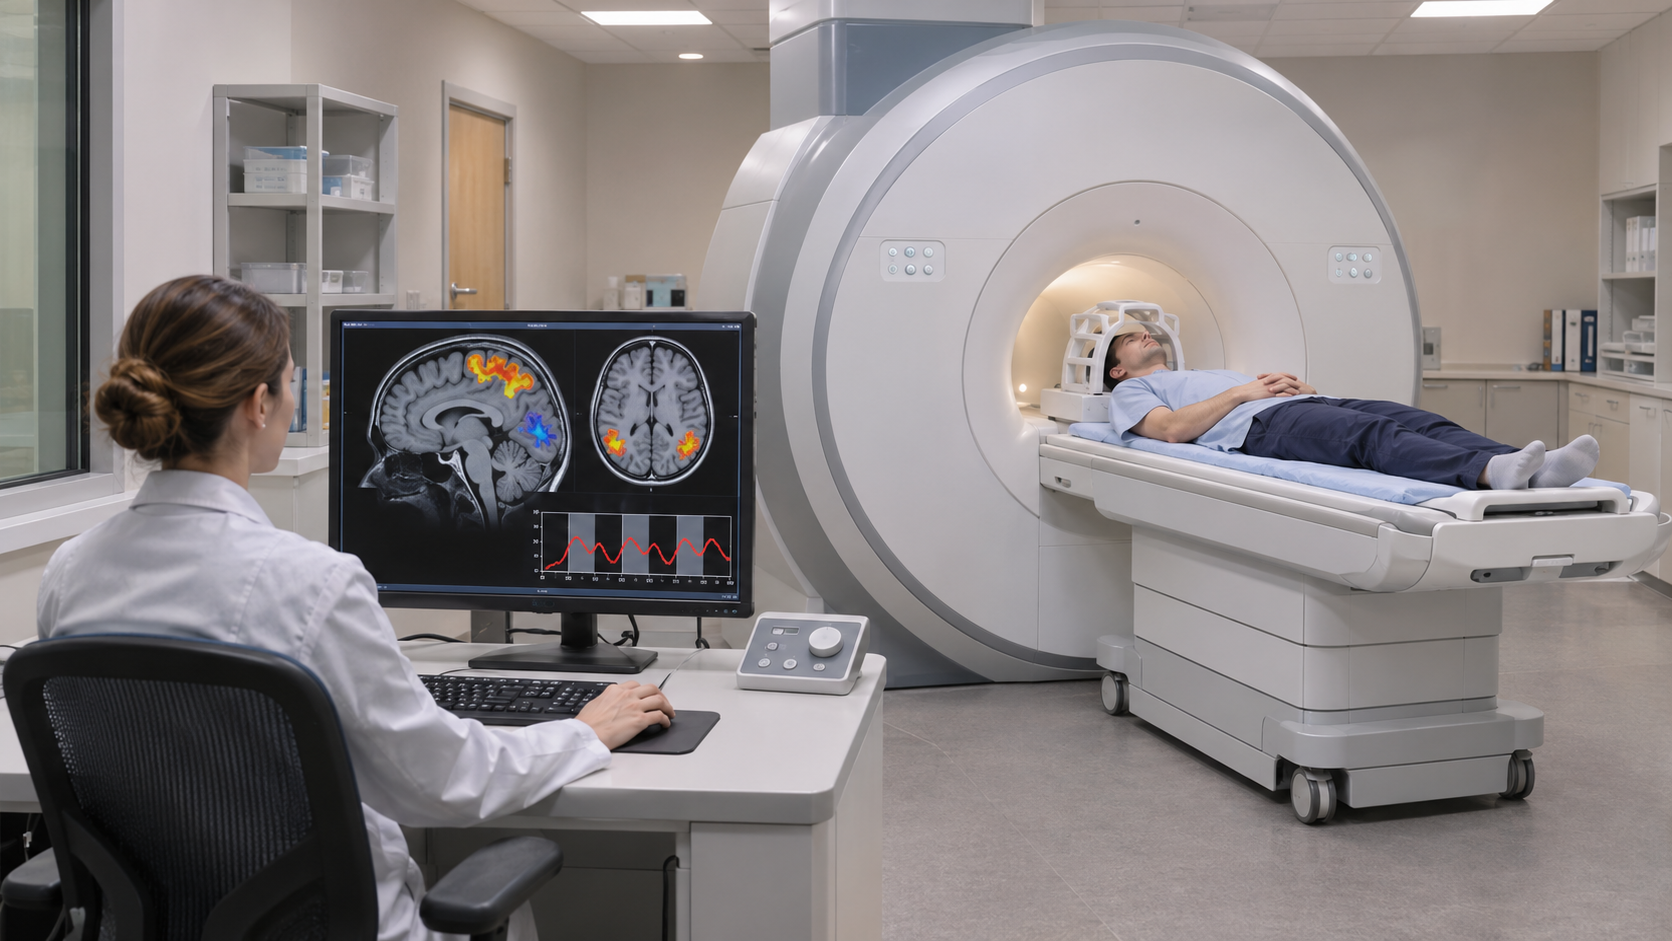
\includegraphics[width=\textwidth,keepaspectratio]{modalities/infographics/fmri_realistic.png}
\end{center}
\begin{center}\footnotesize BOLD fMRI maps task-related changes in blood oxygenation, an indirect hemodynamic signal rather than a direct recording of neuronal firing. AI-generated illustration; activation maps are not research data.\end{center}

\section{Overview}
Functional magnetic resonance imaging (fMRI) is a specialized MRI technique that measures changes in blood oxygenation and hemodynamics associated with neuronal activity. Most clinical and research applications use the blood oxygen level-dependent (BOLD) signal.

Unlike conventional MRI, which primarily examines anatomical and pathological abnormalities, fMRI investigates functional localization of brain regions, functional connectivity, reorganization of neural networks, abnormal activation patterns, cognitive, sensory and motor functions, and hemodynamic responses associated with neuronal activity.

fMRI is predominantly a research modality, with relatively limited routine clinical applications. Presurgical motor and language mapping are established clinical uses in selected cases. Many reported associations in the catalogues below are group-level research findings and are not validated as individual diagnostic tests.

 Individual findings have not been independently verified against published studies or clinical guidelines.

\section{Where fMRI is used}
The numbered entries summarize examples of conditions studied with fMRI and reported functional patterns. Findings are influenced by task design, patient performance, head motion, vascular physiology, acquisition parameters, and analysis methods.

\subsection{Brain tumors and presurgical planning}
\begin{enumerate}[leftmargin=*,itemsep=0.45em,topsep=0.4em]
\item \textbf{Astrocytoma.} Useful imaging findings include: Altered activation near tumor boundaries.
\item \textbf{Brain metastases.} Useful imaging findings include: Altered activation near metastatic lesions.
\item \textbf{Brainstem tumors.} Useful imaging findings include: Possible alterations in functional networks.
\item \textbf{Cavernous malformation.} Useful imaging findings include: Functional cortical activation adjacent to the lesion.
\item \textbf{Cerebral arteriovenous malformation.} Useful imaging findings include: Altered functional localization and neurovascular coupling.
\item \textbf{Glioblastoma.} Useful imaging findings include: Displacement or reorganization of functional cortical regions.
\item \textbf{Low-grade glioma.} Useful imaging findings include: Functional cortical reorganization.
\item \textbf{Meningioma.} Useful imaging findings include: Displacement of functional cortical regions.
\item \textbf{Oligodendroglioma.} Useful imaging findings include: Reorganization of functional cortical networks.
\end{enumerate}
The principal purpose in these cases is to identify functionally important brain regions before surgery, rather than to diagnose the tumor itself.

\subsection{Epilepsy}
\begin{enumerate}[leftmargin=*,itemsep=0.45em,topsep=0.4em]
\item \textbf{Childhood absence epilepsy.} Useful imaging findings include: Altered thalamocortical network activity.
\item \textbf{Drug-resistant epilepsy.} Useful imaging findings include: Functional reorganization of language and memory networks.
\item \textbf{Focal cortical dysplasia.} Useful imaging findings include: Abnormal regional functional activation.
\item \textbf{Focal epilepsy.} Useful imaging findings include: Altered regional functional connectivity.
\item \textbf{Frontal lobe epilepsy.} Useful imaging findings include: Abnormal frontal network activity.
\item \textbf{Generalized epilepsy.} Useful imaging findings include: Abnormal thalamocortical connectivity.
\item \textbf{Juvenile myoclonic epilepsy.} Useful imaging findings include: Altered motor and cognitive network connectivity.
\item \textbf{Lennox--Gastaut syndrome.} Useful imaging findings include: Altered widespread cortical and subcortical networks.
\item \textbf{Mesial temporal sclerosis.} Useful imaging findings include: Altered hippocampal activation and connectivity.
\item \textbf{Temporal lobe epilepsy.} Useful imaging findings include: Altered temporal lobe functional connectivity.
\end{enumerate}
Presurgical language lateralization is an established clinical application. Simultaneous EEG-fMRI for localization of epileptic activity remains more specialized.

\subsection{Cerebrovascular diseases}
\begin{enumerate}[leftmargin=*,itemsep=0.45em,topsep=0.4em]
\item \textbf{Carotid artery stenosis.} Useful imaging findings include: Altered cerebrovascular reactivity.
\item \textbf{Cerebral small vessel disease.} Useful imaging findings include: Reduced or altered functional connectivity.
\item \textbf{Chronic cerebral ischemia.} Useful imaging findings include: Abnormal hemodynamic responses.
\item \textbf{Hemorrhagic stroke.} Useful imaging findings include: Functional network disruption.
\item \textbf{Ischemic stroke.} Useful imaging findings include: Altered activation within affected functional networks.
\item \textbf{Moyamoya disease.} Useful imaging findings include: Impaired or delayed cerebrovascular reactivity.
\item \textbf{Post-stroke aphasia.} Useful imaging findings include: Reorganization of language networks.
\item \textbf{Post-stroke cognitive impairment.} Useful imaging findings include: Altered executive and attention networks.
\item \textbf{Post-stroke motor impairment.} Useful imaging findings include: Altered sensorimotor cortical activation.
\item \textbf{Vascular dementia.} Useful imaging findings include: Disrupted large-scale neural networks.
\end{enumerate}

\subsection{Neurodegenerative diseases}
\begin{enumerate}[leftmargin=*,itemsep=0.45em,topsep=0.4em]
\item \textbf{Alzheimer disease.} Useful imaging findings include: Altered default mode network connectivity.
\item \textbf{Amyotrophic lateral sclerosis.} Useful imaging findings include: Altered motor network connectivity.
\item \textbf{Dementia with Lewy bodies.} Useful imaging findings include: Altered visual and attention networks.
\item \textbf{Frontotemporal dementia.} Useful imaging findings include: Disrupted frontal and temporal networks.
\item \textbf{Huntington disease.} Useful imaging findings include: Altered corticostriatal functional connectivity.
\item \textbf{Mild cognitive impairment.} Useful imaging findings include: Altered hippocampal and cortical connectivity.
\item \textbf{Multiple system atrophy.} Useful imaging findings include: Altered cerebellar and motor connectivity.
\item \textbf{Parkinson disease.} Useful imaging findings include: Abnormal corticostriatal connectivity.
\item \textbf{Posterior cortical atrophy.} Useful imaging findings include: Altered posterior cortical networks.
\item \textbf{Primary progressive aphasia.} Useful imaging findings include: Disrupted language networks.
\item \textbf{Progressive supranuclear palsy.} Useful imaging findings include: Disrupted brainstem and frontal networks.
\item \textbf{Spinocerebellar ataxia.} Useful imaging findings include: Abnormal cerebellocortical connectivity.
\end{enumerate}

\subsection{Psychiatric disorders}
\begin{enumerate}[leftmargin=*,itemsep=0.45em,topsep=0.4em]
\item \textbf{Alcohol use disorder.} Useful imaging findings include: Altered reward and executive networks.
\item \textbf{Anorexia nervosa.} Useful imaging findings include: Altered reward and body perception networks.
\item \textbf{Binge-eating disorder.} Useful imaging findings include: Altered food-related reward responses.
\item \textbf{Bipolar disorder.} Useful imaging findings include: Abnormal emotional regulation networks.
\item \textbf{Borderline personality disorder.} Useful imaging findings include: Altered emotional regulation networks.
\item \textbf{Bulimia nervosa.} Useful imaging findings include: Altered reward and inhibitory control networks.
\item \textbf{Cocaine use disorder.} Useful imaging findings include: Altered reward and inhibitory control networks.
\item \textbf{Gambling disorder.} Useful imaging findings include: Altered reward-processing and decision-making networks.
\item \textbf{Generalized anxiety disorder.} Useful imaging findings include: Altered amygdala-prefrontal connectivity.
\item \textbf{Major depressive disorder.} Useful imaging findings include: Altered limbic and prefrontal connectivity.
\item \textbf{Nicotine dependence.} Useful imaging findings include: Altered cue-related reward network activation.
\item \textbf{Obsessive-compulsive disorder.} Useful imaging findings include: Altered corticostriatal-thalamocortical connectivity.
\item \textbf{Opioid use disorder.} Useful imaging findings include: Altered reward and motivational circuitry.
\item \textbf{Panic disorder.} Useful imaging findings include: Abnormal fear-processing network activity.
\item \textbf{Post-traumatic stress disorder.} Useful imaging findings include: Altered amygdala, hippocampal and prefrontal responses.
\item \textbf{Schizophrenia.} Useful imaging findings include: Disrupted large-scale functional connectivity.
\item \textbf{Social anxiety disorder.} Useful imaging findings include: Altered responses to socially threatening stimuli.
\item \textbf{Specific phobia.} Useful imaging findings include: Increased activation of fear-related networks during exposure.
\end{enumerate}
These disorders cannot currently be reliably diagnosed in an individual patient using fMRI alone. Most reported findings represent statistical differences between research populations.

\subsection{Neurodevelopmental disorders}
\begin{enumerate}[leftmargin=*,itemsep=0.45em,topsep=0.4em]
\item \textbf{Attention deficit hyperactivity disorder.} Useful imaging findings include: Altered attention and executive control networks.
\item \textbf{Autism spectrum disorder.} Useful imaging findings include: Altered social cognition and functional connectivity networks.
\item \textbf{Cerebral palsy.} Useful imaging findings include: Functional reorganization of motor networks.
\item \textbf{Developmental dyscalculia.} Useful imaging findings include: Altered numerical processing networks.
\item \textbf{Developmental dyslexia.} Useful imaging findings include: Altered activation of reading-related networks.
\item \textbf{Developmental language disorder.} Useful imaging findings include: Altered language network activation.
\item \textbf{Down syndrome.} Useful imaging findings include: Altered large-scale functional connectivity.
\item \textbf{Fragile X syndrome.} Useful imaging findings include: Abnormal cognitive and emotional processing networks.
\item \textbf{Rett syndrome.} Useful imaging findings include: Altered sensorimotor and cognitive networks.
\item \textbf{Tourette syndrome.} Useful imaging findings include: Altered corticostriatal motor circuitry.
\item \textbf{Williams syndrome.} Useful imaging findings include: Altered visuospatial and social processing networks.
\end{enumerate}

\subsection{Demyelinating and inflammatory neurological diseases}
\begin{enumerate}[leftmargin=*,itemsep=0.45em,topsep=0.4em]
\item \textbf{Anti-NMDA receptor encephalitis.} Useful imaging findings include: Altered hippocampal and large-scale connectivity.
\item \textbf{Autoimmune encephalitis.} Useful imaging findings include: Disrupted cognitive and limbic networks.
\item \textbf{Multiple sclerosis.} Useful imaging findings include: Altered functional connectivity and compensatory cortical activation.
\item \textbf{Neuromyelitis optica spectrum disorder.} Useful imaging findings include: Altered visual and sensorimotor networks.
\item \textbf{Neuropsychiatric systemic lupus erythematosus.} Useful imaging findings include: Altered cognitive and emotional networks.
\end{enumerate}

\subsection{Traumatic brain injuries and disorders of consciousness}
\begin{enumerate}[leftmargin=*,itemsep=0.45em,topsep=0.4em]
\item \textbf{Cognitive motor dissociation.} Useful imaging findings include: Task-related brain activation despite absent observable behavioral response.
\item \textbf{Diffuse axonal injury.} Useful imaging findings include: Reduced or altered functional network connectivity.
\item \textbf{Disorders of consciousness.} Useful imaging findings include: Altered default mode and frontoparietal networks.
\item \textbf{Hypoxic brain injury.} Useful imaging findings include: Disrupted cortical and subcortical connectivity.
\item \textbf{Mild traumatic brain injury.} Useful imaging findings include: Altered functional connectivity.
\item \textbf{Minimally conscious state.} Useful imaging findings include: Variable preservation of higher-order functional networks.
\item \textbf{Moderate traumatic brain injury.} Useful imaging findings include: Disruption of large-scale neural networks.
\item \textbf{Post-concussion syndrome.} Useful imaging findings include: Altered attention and executive networks.
\item \textbf{Severe traumatic brain injury.} Useful imaging findings include: Extensive functional network abnormalities.
\item \textbf{Unresponsive wakefulness syndrome.} Useful imaging findings include: Reduced connectivity in consciousness-related networks; occasional covert task responses.
\end{enumerate}
Assessment of covert consciousness is an important emerging clinical application of task-based fMRI.

\subsection{Chronic pain and headache disorders}
\begin{enumerate}[leftmargin=*,itemsep=0.45em,topsep=0.4em]
\item \textbf{Chronic lower back pain.} Useful imaging findings include: Altered pain and emotional processing networks.
\item \textbf{Chronic pelvic pain.} Useful imaging findings include: Altered central pain-processing connectivity.
\item \textbf{Cluster headache.} Useful imaging findings include: Altered hypothalamic network activity.
\item \textbf{Complex regional pain syndrome.} Useful imaging findings include: Altered sensorimotor and pain networks.
\item \textbf{Fibromyalgia.} Useful imaging findings include: Altered central pain-processing networks.
\item \textbf{Irritable bowel syndrome.} Useful imaging findings include: Altered brain-gut processing networks.
\item \textbf{Migraine.} Useful imaging findings include: Altered sensory and pain-processing networks.
\item \textbf{Migraine with aura.} Useful imaging findings include: Altered visual cortical activity and hemodynamic responses.
\item \textbf{Neuropathic pain.} Useful imaging findings include: Abnormal somatosensory and pain-related connectivity.
\item \textbf{Phantom limb pain.} Useful imaging findings include: Altered sensorimotor cortical organization.
\item \textbf{Temporomandibular disorders.} Useful imaging findings include: Altered central pain-processing networks.
\item \textbf{Trigeminal neuralgia.} Useful imaging findings include: Altered pain-processing network activity.
\end{enumerate}

\subsection{Sensory disorders}
\begin{enumerate}[leftmargin=*,itemsep=0.45em,topsep=0.4em]
\item \textbf{Acquired blindness.} Useful imaging findings include: Altered visual cortical connectivity.
\item \textbf{Amblyopia.} Useful imaging findings include: Reduced or altered visual cortical responses.
\item \textbf{Anosmia.} Useful imaging findings include: Reduced olfactory-related cortical activation.
\item \textbf{Congenital blindness.} Useful imaging findings include: Cross-modal reorganization of the visual cortex.
\item \textbf{Congenital deafness.} Useful imaging findings include: Cross-modal reorganization of auditory regions.
\item \textbf{Glaucoma.} Useful imaging findings include: Altered visual pathway functional connectivity.
\item \textbf{Optic neuritis.} Useful imaging findings include: Altered visual cortical activation.
\item \textbf{Sensorineural hearing loss.} Useful imaging findings include: Altered auditory cortical activity.
\item \textbf{Tinnitus.} Useful imaging findings include: Altered auditory and limbic network activity.
\item \textbf{Vestibular disorders.} Useful imaging findings include: Altered vestibular processing networks.
\end{enumerate}

\subsection{Sleep disorders}
\begin{enumerate}[leftmargin=*,itemsep=0.45em,topsep=0.4em]
\item \textbf{Chronic insomnia.} Useful imaging findings include: Altered arousal and default mode networks.
\item \textbf{Narcolepsy.} Useful imaging findings include: Altered arousal and sleep regulation networks.
\item \textbf{Obstructive sleep apnea.} Useful imaging findings include: Altered cognitive and executive networks.
\item \textbf{REM sleep behavior disorder.} Useful imaging findings include: Altered motor and brainstem-associated networks.
\item \textbf{Restless legs syndrome.} Useful imaging findings include: Altered sensorimotor connectivity.
\end{enumerate}

\subsection{Metabolic and systemic diseases}
\begin{enumerate}[leftmargin=*,itemsep=0.45em,topsep=0.4em]
\item \textbf{Chronic kidney disease.} Useful imaging findings include: Altered cognitive network connectivity.
\item \textbf{Hepatic encephalopathy.} Useful imaging findings include: Disrupted large-scale functional connectivity.
\item \textbf{HIV-associated neurocognitive disorders.} Useful imaging findings include: Altered executive and cognitive networks.
\item \textbf{Long COVID.} Useful imaging findings include: Reported alterations in functional connectivity.
\item \textbf{Myalgic encephalomyelitis/chronic fatigue syndrome.} Useful imaging findings include: Reported alterations in cognitive and other functional networks.
\item \textbf{Obesity.} Useful imaging findings include: Altered reward and food-processing networks.
\item \textbf{Type 1 diabetes mellitus.} Useful imaging findings include: Altered cognitive and functional connectivity patterns.
\item \textbf{Type 2 diabetes mellitus.} Useful imaging findings include: Altered hippocampal and default mode connectivity.
\end{enumerate}

\subsection{Summary of catalogue}
\begin{center}
\begin{tabular}{@{}p{0.70\textwidth}r@{}}
\toprule
\textbf{Disease category} & \textbf{Entries} \\
\midrule
Brain tumors and presurgical planning & 9 \\
Cerebrovascular diseases & 10 \\
Chronic pain and headache disorders & 12 \\
Demyelinating and inflammatory diseases & 5 \\
Epilepsy & 10 \\
Metabolic and systemic diseases & 8 \\
Neurodegenerative diseases & 12 \\
Neurodevelopmental disorders & 11 \\
Psychiatric disorders & 18 \\
Sensory disorders & 10 \\
Sleep disorders & 5 \\
Traumatic brain injuries and consciousness disorders & 10 \\
\midrule
\textbf{Total} & \textbf{120} \\
\bottomrule
\end{tabular}
\end{center}

\subsection{Types of functional MRI}
\begin{longtable}{@{}p{0.36\textwidth}p{0.58\textwidth}@{}}
\toprule
\textbf{Technique} & \textbf{Primary application} \\
\midrule
\endfirsthead
\toprule
\textbf{Technique} & \textbf{Primary application} \\
\midrule
\endhead
Arterial spin labeling (ASL) & Measurement of cerebral blood flow \\
BOLD fMRI & Blood oxygenation-dependent functional assessment \\
Calibrated fMRI & Estimation of physiological parameters associated with brain activation \\
Cerebrovascular reactivity MRI & Assessment of vascular responses to physiological stimuli \\
EEG-fMRI & Correlation between electrophysiological and hemodynamic activity \\
Multi-echo fMRI & Improved separation of BOLD signals from certain artifacts \\
Pharmacological fMRI & Brain responses to pharmacological agents \\
Real-time fMRI & Neurofeedback and real-time functional monitoring \\
Resting-state fMRI (rs-fMRI) & Intrinsic functional connectivity \\
Task-based fMRI & Functional localization during specific tasks \\
\bottomrule
\end{longtable}

\subsection{Major functional brain networks}
\begin{longtable}{@{}p{0.36\textwidth}p{0.58\textwidth}@{}}
\toprule
\textbf{Functional network} & \textbf{Primary function} \\
\midrule
\endfirsthead
\toprule
Auditory network & Auditory processing \\
\midrule
\endhead
Central executive network (CEN) & Executive function and working memory \\
Cerebellar networks & Motor coordination and cognitive processing \\
Default mode network (DMN) & Internally directed cognition \\
Dorsal attention network (DAN) & Goal-directed attention \\
\textbf{Functional network} & \textbf{Primary function} \\
Language network & Language comprehension and production \\
Limbic network & Emotion and memory \\
Reward network & Motivation and reinforcement \\
Salience network (SN) & Detection of behaviorally relevant stimuli \\
Sensorimotor network & Motor and sensory processing \\
Ventral attention network (VAN) & Stimulus-driven attention \\
Visual network & Visual information processing \\
\bottomrule
\end{longtable}

\subsection{Clinical applications versus research applications}
\begin{longtable}{@{}p{0.40\textwidth}p{0.54\textwidth}@{}}
\toprule
\textbf{Application} & \textbf{Clinical status} \\
\midrule
\endfirsthead
\toprule
\textbf{Application} & \textbf{Clinical status} \\
\midrule
\endhead
Brain--computer interfaces & Experimental \\
Cerebrovascular reactivity mapping & Specialized clinical application \\
Chronic pain diagnosis & Experimental \\
Detection of covert consciousness & Emerging clinical application \\
Epileptic activity localization with EEG-fMRI & Specialized and investigational \\
Language lateralization in epilepsy & Established \\
Neurodegenerative disease classification & Predominantly research \\
Neurodevelopmental disease diagnosis & Experimental \\
Presurgical language mapping & Established \\
Presurgical memory mapping & Specialized clinical application \\
Presurgical motor mapping & Established \\
Presurgical sensory mapping & Established in selected cases \\
Psychiatric disease diagnosis & Experimental \\
Stroke rehabilitation assessment & Predominantly research \\
Treatment response prediction & Experimental \\
\bottomrule
\end{longtable}

\subsection{Published fMRI datasets}
\begin{longtable}{@{}p{0.36\textwidth}p{0.58\textwidth}@{}}
\toprule
\textbf{Source} & \textbf{Primary utility} \\
\midrule
\endfirsthead
\toprule
\textbf{Source} & \textbf{Primary utility} \\
\midrule
\endhead
ABIDE & Autism spectrum disorder \\
ADHD-200 & Attention deficit hyperactivity disorder \\
ADNI & Alzheimer disease and cognitive impairment \\
Human Connectome Project & Human functional brain connectivity \\
Neurosynth & Large-scale neuroimaging meta-analysis \\
NeuroVault & Published statistical brain activation maps \\
NITRC & Neuroimaging datasets and computational tools \\
OpenNeuro & Task-based and resting-state fMRI datasets \\
PubMed Central & Published clinical and experimental studies \\
UK Biobank & Population-scale neuroimaging \\
\bottomrule
\end{longtable}

\subsection{Recommended metadata for an fMRI dataset}
\begin{longtable}{@{}p{0.45\textwidth}p{0.49\textwidth}@{}}
\toprule
\textbf{Attribute} & \textbf{Example} \\
\midrule
Acquisition duration & 600 seconds \\
Acquisition paradigm & Task-based \\
Cognitive task & Verbal fluency \\
Dataset organization & BIDS \\
Diagnostic reference standard & Independently established clinical diagnosis \\
Disease & Temporal lobe epilepsy \\
Echo time & 30 ms \\
Functional connectivity & Pearson correlation \\
Functional network & Language network \\
Head motion & Framewise displacement \\
Hemodynamic response function & Canonical HRF \\
Image format & NIfTI \\
Imaging modality & BOLD fMRI \\
Magnetic field strength & 3 Tesla \\
Number of temporal volumes & 300 \\
Publication reference & DOI or PMID \\
Repetition time & 2,000 ms \\
Spatial coordinate system & MNI152 \\
Statistical measurement & Z-score \\
Statistical threshold & FDR-corrected $p < 0.05$ \\
Voxel dimensions & $2 \times 2 \times 2$ mm \\
\bottomrule
\end{longtable}

\subsection{Imaging dimensionality and research considerations}
Unlike conventional MRI, fMRI is fundamentally a four-dimensional spatiotemporal imaging modality.
\begin{center}
\begin{tabular}{@{}ll@{}}
\toprule
\textbf{Modality} & \textbf{Data dimensionality} \\
\midrule
Conventional ultrasound & $X, Y$; optionally time \\
Conventional X-ray & $X, Y$ \\
CT & $X, Y, Z$ \\
Echocardiography & $X, Y$, time; optionally $Z$ \\
fMRI & $X, Y, Z$, time \\
Mammography & $X, Y$ \\
Structural MRI & $X, Y, Z$ \\
\bottomrule
\end{tabular}
\end{center}

The colored regions in an fMRI image are generally pseudocolored statistical or quantitative maps superimposed on structural brain images. They are not direct photographs of neuronal activity. For AI-based medical image diagnosis, fMRI is substantially less suitable than structural MRI or CT when the input consists exclusively of static images. Analysis generally requires temporal signals, statistical parametric maps, functional connectivity matrices, and acquisition metadata.


\chapter{Diffusion Magnetic Resonance Imaging (dMRI)}
\label{ch:diffusion_mri}

% Chapter-opening illustrated modality infographic.
\begin{center}
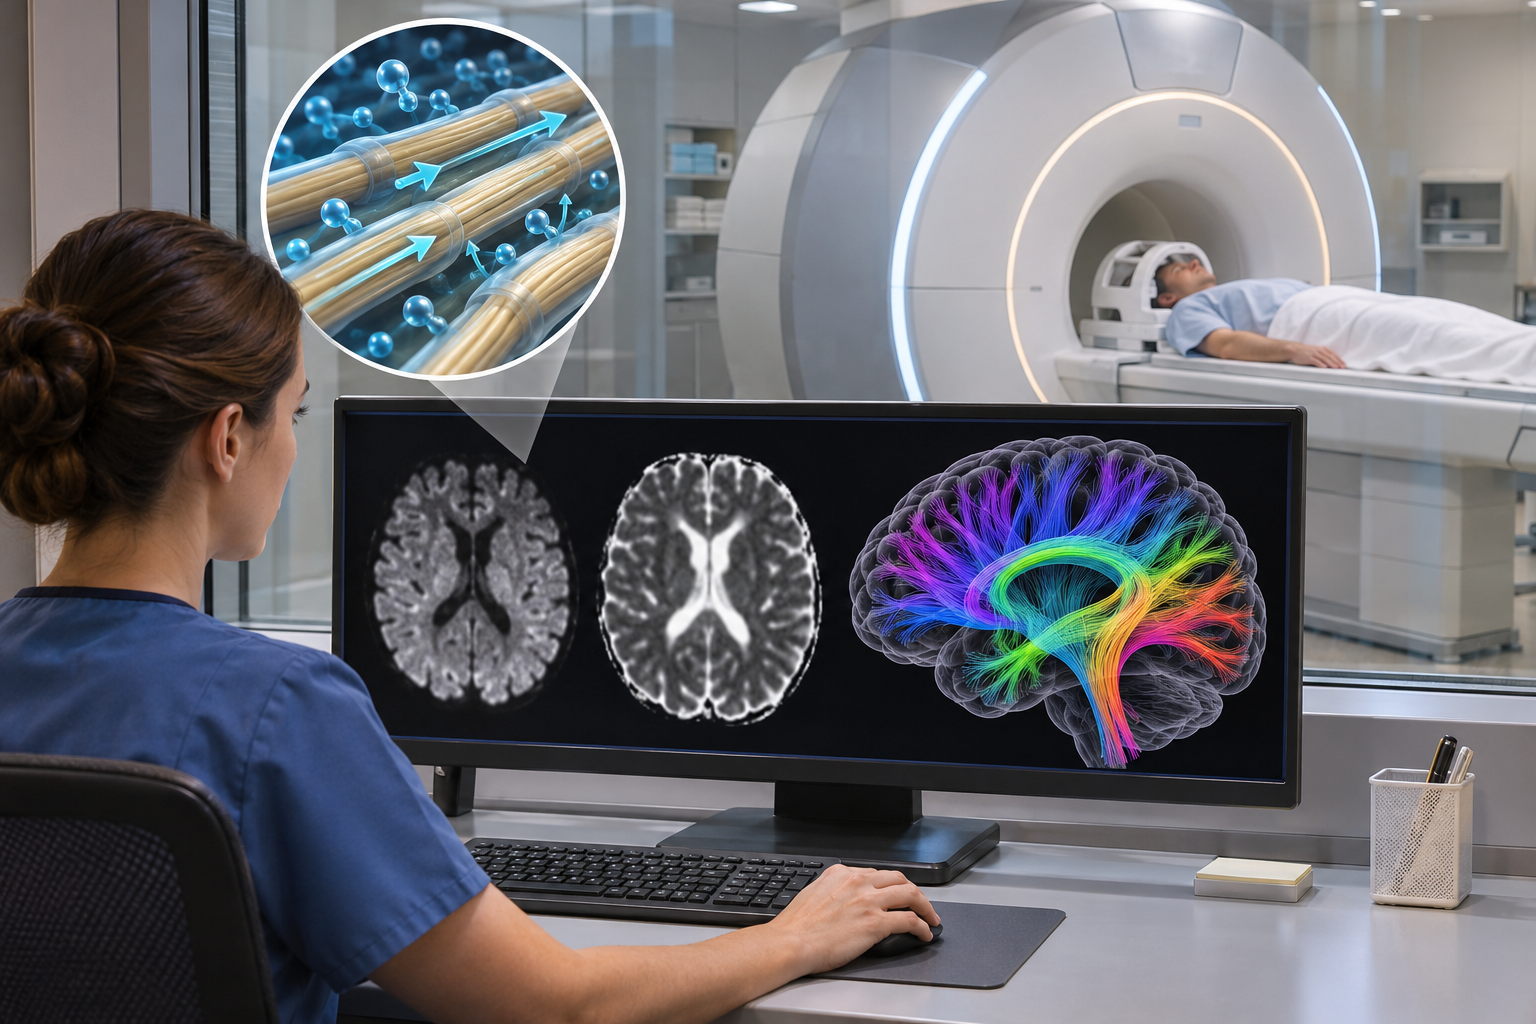
\includegraphics[width=\textwidth,keepaspectratio]{modalities/infographics/dmri_realistic.png}
\end{center}
\begin{center}\footnotesize Diffusion MRI is sensitive to microscopic water motion; DWI and ADC should be interpreted together, while tractography is model-derived. AI-generated illustration; displayed maps are not clinical studies.\end{center}

\section{Overview}
Diffusion magnetic resonance imaging (dMRI) is a specialized MRI technique that measures the microscopic movement of water molecules within biological tissues. This movement is influenced by cellular membranes, tissue microstructure, cellular density, viscosity, and the orientation of nerve fibers.

Unlike conventional MRI, which primarily provides anatomical information, diffusion MRI provides information about tissue microstructure and pathological changes that may not be visible on conventional MRI. It is particularly valuable for detecting acute cerebral ischemia, malignant tumors with high cellularity, abscesses and infections, white-matter injuries, demyelinating diseases, abnormalities of neural fiber pathways, and tumor response to treatment.

The 217 entries are a preliminary catalogue of diseases and conditions evaluated or investigated using diffusion MRI. They are not 217 independently validated clinical indications. Individual guideline and literature verification is necessary before using them as diagnostic ground truth.

\section{Where diffusion MRI is used}
The numbered entries give examples of reported diffusion MRI findings. Interpretation depends on acquisition technique, b-values, gradient directions, image quality, diffusion model, and correlation with ADC maps and other MRI sequences.

\subsection{Cerebrovascular diseases}
\begin{enumerate}[leftmargin=*,itemsep=0.45em,topsep=0.4em]
\item \textbf{Acute ischemic stroke.} Useful imaging findings include: Increased DWI signal and reduced ADC.
\item \textbf{Brainstem infarction.} Useful imaging findings include: Focal restricted diffusion within the brainstem.
\item \textbf{CADASIL.} Useful imaging findings include: Abnormal white-matter diffusion metrics.
\item \textbf{Cerebellar infarction.} Useful imaging findings include: Restricted diffusion within cerebellar tissue.
\item \textbf{Cerebral small vessel disease.} Useful imaging findings include: Reduced fractional anisotropy in affected white matter.
\item \textbf{Cerebral venous infarction.} Useful imaging findings include: Variable diffusion restriction and vasogenic edema.
\item \textbf{Delayed posthypoxic leukoencephalopathy.} Useful imaging findings include: Diffuse white-matter diffusion restriction.
\item \textbf{Global cerebral ischemia.} Useful imaging findings include: Widespread diffusion abnormalities.
\item \textbf{Hyperacute cerebral infarction.} Useful imaging findings include: Early diffusion restriction.
\item \textbf{Hypoxic-ischemic encephalopathy.} Useful imaging findings include: Cortical or deep gray-matter diffusion restriction.
\item \textbf{Lacunar infarction.} Useful imaging findings include: Small focal area of restricted diffusion.
\item \textbf{Moyamoya disease.} Useful imaging findings include: Ischemic lesions and altered white-matter integrity.
\item \textbf{Multiple embolic infarctions.} Useful imaging findings include: Multiple scattered areas of restricted diffusion.
\item \textbf{Posterior reversible encephalopathy syndrome.} Useful imaging findings include: Typically increased ADC due to vasogenic edema.
\item \textbf{Watershed infarction.} Useful imaging findings include: Restricted diffusion in arterial border zones.
\end{enumerate}
Acute ischemic stroke is among the most important and established clinical applications of diffusion MRI. DWI can be negative early, particularly with small or posterior-circulation infarcts; a negative scan does not exclude stroke when clinical suspicion remains. MRI should not delay time-critical treatment.

\subsection{Brain tumors}
\begin{enumerate}[leftmargin=*,itemsep=0.45em,topsep=0.4em]
\item \textbf{Atypical teratoid/rhabdoid tumor.} Useful imaging findings include: Restricted diffusion in solid components.
\item \textbf{Brain metastases.} Useful imaging findings include: Variable diffusion characteristics.
\item \textbf{Diffuse astrocytoma.} Useful imaging findings include: Variable ADC values.
\item \textbf{Embryonal tumor with multilayered rosettes.} Useful imaging findings include: Marked diffusion restriction.
\item \textbf{Ependymoma.} Useful imaging findings include: Variable diffusion restriction.
\item \textbf{Epidermoid cyst.} Useful imaging findings include: Characteristically increased DWI signal with reduced ADC relative to CSF.
\item \textbf{Germinoma.} Useful imaging findings include: Frequently reduced ADC.
\item \textbf{Glioblastoma.} Useful imaging findings include: Heterogeneous diffusion with restricted regions in cellular components.
\item \textbf{Hemangioblastoma.} Useful imaging findings include: Generally facilitated diffusion in solid components.
\item \textbf{Medulloblastoma.} Useful imaging findings include: Restricted diffusion associated with high cellularity.
\item \textbf{Meningioma.} Useful imaging findings include: Variable ADC, sometimes reduced in higher-grade tumors.
\item \textbf{Oligodendroglioma.} Useful imaging findings include: Variable intratumoral diffusion characteristics.
\item \textbf{Pilocytic astrocytoma.} Useful imaging findings include: Generally higher ADC in less cellular components.
\item \textbf{Pineoblastoma.} Useful imaging findings include: Restricted diffusion.
\item \textbf{Primary CNS lymphoma.} Useful imaging findings include: Markedly restricted diffusion.
\item \textbf{Radiation necrosis.} Useful imaging findings include: Variable diffusion characteristics, often overlapping with recurrence.
\item \textbf{Recurrent brain tumor.} Useful imaging findings include: Possible reduced ADC in viable tumor tissue.
\item \textbf{Vestibular schwannoma.} Useful imaging findings include: Variable diffusion characteristics.
\end{enumerate}
Diffusion measurements can support tumor characterization but cannot reliably establish histological or molecular tumor classification independently.

\subsection{Central nervous system infections}
\begin{enumerate}[leftmargin=*,itemsep=0.45em,topsep=0.4em]
\item \textbf{Cerebral malaria.} Useful imaging findings include: Variable cortical and white-matter diffusion abnormalities.
\item \textbf{Cerebral toxoplasmosis.} Useful imaging findings include: Variable diffusion characteristics.
\item \textbf{Epidural empyema.} Useful imaging findings include: Restricted diffusion within infectious collection.
\item \textbf{Fungal cerebral abscess.} Useful imaging findings include: Variable peripheral or central diffusion restriction.
\item \textbf{Herpes simplex encephalitis.} Useful imaging findings include: Restricted diffusion in temporal and insular regions.
\item \textbf{Intracranial tuberculoma.} Useful imaging findings include: Variable diffusion restriction depending on lesion composition.
\item \textbf{Japanese encephalitis.} Useful imaging findings include: Variable thalamic and deep gray-matter diffusion abnormalities.
\item \textbf{Progressive multifocal leukoencephalopathy.} Useful imaging findings include: Restricted diffusion at active lesion margins.
\item \textbf{Pyogenic cerebral abscess.} Useful imaging findings include: Marked central diffusion restriction.
\item \textbf{Subdural empyema.} Useful imaging findings include: Restricted diffusion within purulent collection.
\item \textbf{Tuberculous abscess.} Useful imaging findings include: Restricted diffusion within purulent material.
\item \textbf{Ventriculitis.} Useful imaging findings include: Restricted diffusion within ventricular debris.
\item \textbf{West Nile encephalitis.} Useful imaging findings include: Possible diffusion restriction in affected neural structures.
\end{enumerate}

\subsection{Demyelinating and white-matter diseases}
\begin{enumerate}[leftmargin=*,itemsep=0.45em,topsep=0.4em]
\item \textbf{Acute disseminated encephalomyelitis.} Useful imaging findings include: Variable diffusion abnormalities.
\item \textbf{Alexander disease.} Useful imaging findings include: Altered white-matter diffusion characteristics.
\item \textbf{Canavan disease.} Useful imaging findings include: Abnormal white-matter diffusion.
\item \textbf{Krabbe disease.} Useful imaging findings include: Altered diffusion in affected white-matter tracts.
\item \textbf{Metachromatic leukodystrophy.} Useful imaging findings include: Abnormal white-matter diffusion metrics.
\item \textbf{MOG antibody-associated disease.} Useful imaging findings include: Variable lesional diffusion abnormalities.
\item \textbf{Multiple sclerosis.} Useful imaging findings include: Altered ADC and reduced fractional anisotropy.
\item \textbf{Neuromyelitis optica spectrum disorder.} Useful imaging findings include: Altered diffusion within affected neural pathways.
\item \textbf{Osmotic demyelination syndrome.} Useful imaging findings include: Early diffusion restriction in affected regions.
\item \textbf{Toxic leukoencephalopathy.} Useful imaging findings include: Symmetric white-matter diffusion restriction.
\item \textbf{Vanishing white matter disease.} Useful imaging findings include: Increased diffusivity in degenerating white matter.
\item \textbf{X-linked adrenoleukodystrophy.} Useful imaging findings include: Abnormal diffusion within demyelinating regions.
\end{enumerate}

\subsection{Neurodegenerative diseases}
\begin{enumerate}[leftmargin=*,itemsep=0.45em,topsep=0.4em]
\item \textbf{Alzheimer disease.} Useful imaging findings include: Reduced white-matter integrity and altered diffusivity.
\item \textbf{Amyotrophic lateral sclerosis.} Useful imaging findings include: Reduced fractional anisotropy in corticospinal tracts.
\item \textbf{Creutzfeldt--Jakob disease.} Useful imaging findings include: Cortical ribboning and basal ganglia diffusion restriction.
\item \textbf{Dementia with Lewy bodies.} Useful imaging findings include: Altered white-matter microstructure.
\item \textbf{Friedreich ataxia.} Useful imaging findings include: Altered diffusion in cerebellar and spinal pathways.
\item \textbf{Frontotemporal dementia.} Useful imaging findings include: Abnormal frontal and temporal white-matter diffusion.
\item \textbf{Huntington disease.} Useful imaging findings include: Altered corticostriatal diffusion metrics.
\item \textbf{Mild cognitive impairment.} Useful imaging findings include: Altered hippocampal and white-matter diffusion metrics.
\item \textbf{Multiple system atrophy.} Useful imaging findings include: Increased diffusivity in affected subcortical structures.
\item \textbf{Parkinson disease.} Useful imaging findings include: Altered diffusion in nigrostriatal pathways.
\item \textbf{Primary lateral sclerosis.} Useful imaging findings include: Altered corticospinal tract integrity.
\item \textbf{Progressive supranuclear palsy.} Useful imaging findings include: Abnormal brainstem diffusion metrics.
\item \textbf{Spinocerebellar ataxia.} Useful imaging findings include: Altered cerebellar white-matter integrity.
\item \textbf{Wilson disease.} Useful imaging findings include: Abnormal diffusion within basal ganglia.
\end{enumerate}
Except for selected conditions such as Creutzfeldt--Jakob disease, most diffusion biomarkers in neurodegenerative diseases remain supplementary or investigational.

\subsection{Traumatic brain injuries}
\begin{enumerate}[leftmargin=*,itemsep=0.45em,topsep=0.4em]
\item \textbf{Cerebral contusion.} Useful imaging findings include: Variable diffusion restriction and edema.
\item \textbf{Diffuse axonal injury.} Useful imaging findings include: Abnormal diffusion within injured white-matter tracts.
\item \textbf{Mild traumatic brain injury.} Useful imaging findings include: Variable white-matter diffusion metrics.
\item \textbf{Moderate traumatic brain injury.} Useful imaging findings include: Altered white-matter microstructure.
\item \textbf{Post-concussion syndrome.} Useful imaging findings include: Reported alterations in white-matter integrity.
\item \textbf{Severe traumatic brain injury.} Useful imaging findings include: Widespread diffusion abnormalities.
\item \textbf{Traumatic brainstem injury.} Useful imaging findings include: Abnormal diffusion within brainstem pathways.
\item \textbf{Traumatic corpus callosum injury.} Useful imaging findings include: Altered callosal diffusion characteristics.
\end{enumerate}

\subsection{Neurodevelopmental and psychiatric disorders}
\begin{enumerate}[leftmargin=*,itemsep=0.45em,topsep=0.4em]
\item \textbf{Attention deficit hyperactivity disorder.} Useful imaging findings include: Altered diffusion in executive control pathways.
\item \textbf{Autism spectrum disorder.} Useful imaging findings include: Reported alterations in white-matter connectivity.
\item \textbf{Bipolar disorder.} Useful imaging findings include: Altered frontolimbic white-matter integrity.
\item \textbf{Cerebral palsy.} Useful imaging findings include: Abnormal corticospinal tract development.
\item \textbf{Developmental dyslexia.} Useful imaging findings include: Altered language-related white-matter tracts.
\item \textbf{Down syndrome.} Useful imaging findings include: Altered white-matter development.
\item \textbf{Fragile X syndrome.} Useful imaging findings include: Abnormal white-matter microstructure.
\item \textbf{Major depressive disorder.} Useful imaging findings include: Reported abnormalities in frontolimbic connectivity.
\item \textbf{Obsessive-compulsive disorder.} Useful imaging findings include: Altered corticostriatal white-matter pathways.
\item \textbf{Post-traumatic stress disorder.} Useful imaging findings include: Altered limbic white-matter connectivity.
\item \textbf{Schizophrenia.} Useful imaging findings include: Reduced fractional anisotropy in selected white-matter pathways.
\item \textbf{Tourette syndrome.} Useful imaging findings include: Altered corticostriatal diffusion metrics.
\end{enumerate}
These applications are predominantly research-oriented. Diffusion MRI cannot independently diagnose these psychiatric or neurodevelopmental disorders.

\subsection{Spinal cord and peripheral nerves}
\begin{enumerate}[leftmargin=*,itemsep=0.45em,topsep=0.4em]
\item \textbf{Brachial plexus injury.} Useful imaging findings include: Altered diffusion and fiber tract continuity.
\item \textbf{Carpal tunnel syndrome.} Useful imaging findings include: Altered median nerve diffusion metrics.
\item \textbf{Cervical spondylotic myelopathy.} Useful imaging findings include: Reduced fractional anisotropy.
\item \textbf{Compressive myelopathy.} Useful imaging findings include: Altered spinal cord diffusion metrics.
\item \textbf{Diabetic peripheral neuropathy.} Useful imaging findings include: Reported changes in peripheral nerve diffusion metrics.
\item \textbf{Multiple sclerosis of the spinal cord.} Useful imaging findings include: Abnormal diffusion in demyelinating lesions.
\item \textbf{Spinal cord infarction.} Useful imaging findings include: Restricted intramedullary diffusion.
\item \textbf{Spinal cord tumors.} Useful imaging findings include: Variable ADC and displacement of neural tracts.
\item \textbf{Transverse myelitis.} Useful imaging findings include: Variable intramedullary diffusion abnormalities.
\item \textbf{Traumatic spinal cord injury.} Useful imaging findings include: Altered diffusion within injured spinal pathways.
\item \textbf{Ulnar nerve entrapment.} Useful imaging findings include: Abnormal diffusion within the affected nerve.
\end{enumerate}

\subsection{Head and neck diseases}
\begin{enumerate}[leftmargin=*,itemsep=0.45em,topsep=0.4em]
\item \textbf{Cholesteatoma.} Useful imaging findings include: Marked DWI hyperintensity on dedicated sequences.
\item \textbf{Deep neck abscess.} Useful imaging findings include: Central diffusion restriction.
\item \textbf{Head and neck lymphoma.} Useful imaging findings include: Marked diffusion restriction.
\item \textbf{Laryngeal carcinoma.} Useful imaging findings include: Reduced tumor ADC.
\item \textbf{Malignant salivary gland tumor.} Useful imaging findings include: Variable or reduced ADC.
\item \textbf{Metastatic cervical lymphadenopathy.} Useful imaging findings include: Variable diffusion restriction.
\item \textbf{Nasopharyngeal carcinoma.} Useful imaging findings include: Reduced ADC in cellular tumor regions.
\item \textbf{Oral squamous cell carcinoma.} Useful imaging findings include: Restricted diffusion in viable tumor.
\item \textbf{Orbital lymphoma.} Useful imaging findings include: Marked diffusion restriction.
\item \textbf{Pleomorphic adenoma.} Useful imaging findings include: Generally higher ADC than highly cellular tumors.
\item \textbf{Retinoblastoma.} Useful imaging findings include: Restricted diffusion within solid tumor.
\item \textbf{Warthin tumor.} Useful imaging findings include: Frequently low ADC.
\end{enumerate}

\subsection{Breast diseases}
\begin{enumerate}[leftmargin=*,itemsep=0.45em,topsep=0.4em]
\item \textbf{Breast abscess.} Useful imaging findings include: Restricted diffusion within purulent material.
\item \textbf{Breast cancer response to chemotherapy.} Useful imaging findings include: Often increased ADC following effective treatment.
\item \textbf{Breast lymphoma.} Useful imaging findings include: Marked diffusion restriction.
\item \textbf{Ductal carcinoma in situ.} Useful imaging findings include: Variable ADC depending on cellularity.
\item \textbf{Fibroadenoma.} Useful imaging findings include: Frequently higher ADC than malignant lesions.
\item \textbf{Invasive ductal carcinoma.} Useful imaging findings include: Frequently reduced ADC.
\item \textbf{Invasive lobular carcinoma.} Useful imaging findings include: Variable diffusion restriction.
\item \textbf{Phyllodes tumor.} Useful imaging findings include: Variable diffusion characteristics.
\item \textbf{Residual breast cancer.} Useful imaging findings include: Persistent diffusion restriction in some viable tumor regions.
\item \textbf{Triple-negative breast cancer.} Useful imaging findings include: Heterogeneous diffusion characteristics.
\end{enumerate}

\subsection{Liver and biliary diseases}
\begin{enumerate}[leftmargin=*,itemsep=0.45em,topsep=0.4em]
\item \textbf{Extrahepatic cholangiocarcinoma.} Useful imaging findings include: Restricted diffusion in affected tissue.
\item \textbf{Focal nodular hyperplasia.} Useful imaging findings include: Variable diffusion characteristics.
\item \textbf{Gallbladder carcinoma.} Useful imaging findings include: Restricted diffusion within malignant tissue.
\item \textbf{Hepatic adenoma.} Useful imaging findings include: Variable ADC.
\item \textbf{Hepatic hemangioma.} Useful imaging findings include: Generally high ADC despite possible DWI hyperintensity.
\item \textbf{Hepatic metastases.} Useful imaging findings include: Restricted diffusion, particularly in viable cellular regions.
\item \textbf{Hepatocellular carcinoma.} Useful imaging findings include: Frequently restricted diffusion in viable tumor.
\item \textbf{Intrahepatic cholangiocarcinoma.} Useful imaging findings include: Restricted diffusion in solid tumor components.
\item \textbf{Liver abscess.} Useful imaging findings include: Central diffusion restriction.
\item \textbf{Liver cirrhosis.} Useful imaging findings include: Altered parenchymal diffusion metrics.
\item \textbf{Liver fibrosis.} Useful imaging findings include: Possible reduction in ADC.
\item \textbf{Simple hepatic cyst.} Useful imaging findings include: Facilitated diffusion.
\end{enumerate}

\subsection{Pancreatic diseases}
\begin{enumerate}[leftmargin=*,itemsep=0.45em,topsep=0.4em]
\item \textbf{Acute pancreatitis.} Useful imaging findings include: Altered pancreatic diffusion.
\item \textbf{Autoimmune pancreatitis.} Useful imaging findings include: Diffuse or focal diffusion restriction.
\item \textbf{Chronic pancreatitis.} Useful imaging findings include: Variable reduction in ADC.
\item \textbf{Intraductal papillary mucinous neoplasm.} Useful imaging findings include: Variable restriction in suspicious solid components.
\item \textbf{Pancreatic abscess.} Useful imaging findings include: Restricted diffusion within purulent material.
\item \textbf{Pancreatic ductal adenocarcinoma.} Useful imaging findings include: Frequently reduced ADC.
\item \textbf{Pancreatic neuroendocrine tumor.} Useful imaging findings include: Variable diffusion restriction.
\item \textbf{Solid pseudopapillary neoplasm.} Useful imaging findings include: Variable diffusion in solid components.
\end{enumerate}

\subsection{Gastrointestinal diseases}
\begin{enumerate}[leftmargin=*,itemsep=0.45em,topsep=0.4em]
\item \textbf{Active Crohn disease.} Useful imaging findings include: Restricted diffusion within inflamed bowel wall.
\item \textbf{Acute appendicitis.} Useful imaging findings include: Possible diffusion restriction in inflamed appendix.
\item \textbf{Anal carcinoma.} Useful imaging findings include: Restricted diffusion in tumor tissue.
\item \textbf{Colorectal carcinoma.} Useful imaging findings include: Reduced tumor ADC.
\item \textbf{Esophageal carcinoma.} Useful imaging findings include: Restricted diffusion in viable tumor.
\item \textbf{Gastric carcinoma.} Useful imaging findings include: Variable tumor diffusion restriction.
\item \textbf{Gastrointestinal lymphoma.} Useful imaging findings include: Marked diffusion restriction.
\item \textbf{Gastrointestinal stromal tumor.} Useful imaging findings include: Variable diffusion characteristics.
\item \textbf{Perianal abscess.} Useful imaging findings include: Restricted diffusion within purulent collection.
\item \textbf{Peritoneal carcinomatosis.} Useful imaging findings include: Diffusion restriction within metastatic deposits.
\item \textbf{Rectal carcinoma.} Useful imaging findings include: Restricted diffusion within viable tumor.
\item \textbf{Residual rectal carcinoma after treatment.} Useful imaging findings include: Persistent focal diffusion restriction in some cases.
\item \textbf{Ulcerative colitis.} Useful imaging findings include: Altered diffusion in inflamed colonic tissue.
\end{enumerate}

\subsection{Renal and urinary diseases}
\begin{enumerate}[leftmargin=*,itemsep=0.45em,topsep=0.4em]
\item \textbf{Acute pyelonephritis.} Useful imaging findings include: Focal or regional diffusion restriction.
\item \textbf{Bladder carcinoma.} Useful imaging findings include: Restricted diffusion within viable tumor.
\item \textbf{Chromophobe renal cell carcinoma.} Useful imaging findings include: Variable or reduced ADC.
\item \textbf{Chronic kidney disease.} Useful imaging findings include: Altered cortical and medullary diffusivity.
\item \textbf{Clear cell renal cell carcinoma.} Useful imaging findings include: Variable ADC.
\item \textbf{Papillary renal cell carcinoma.} Useful imaging findings include: Frequently lower ADC than clear cell carcinoma.
\item \textbf{Renal abscess.} Useful imaging findings include: Marked central diffusion restriction.
\item \textbf{Renal fibrosis.} Useful imaging findings include: Altered renal diffusion parameters.
\item \textbf{Renal infarction.} Useful imaging findings include: Regional diffusion restriction.
\item \textbf{Renal lymphoma.} Useful imaging findings include: Marked diffusion restriction.
\item \textbf{Renal oncocytoma.} Useful imaging findings include: Variable diffusion characteristics.
\item \textbf{Urothelial carcinoma.} Useful imaging findings include: Restricted diffusion within tumor.
\end{enumerate}

\subsection{Female reproductive system}
\begin{enumerate}[leftmargin=*,itemsep=0.45em,topsep=0.4em]
\item \textbf{Adenomyosis.} Useful imaging findings include: Variable myometrial diffusion abnormalities.
\item \textbf{Cellular uterine leiomyoma.} Useful imaging findings include: May show marked diffusion restriction and low ADC, overlapping with leiomyosarcoma.
\item \textbf{Cervical carcinoma.} Useful imaging findings include: Reduced tumor ADC.
\item \textbf{Degenerating uterine fibroid.} Useful imaging findings include: Variable diffusion characteristics.
\item \textbf{Dysgerminoma.} Useful imaging findings include: Restricted diffusion in solid tumor.
\item \textbf{Endometrial carcinoma.} Useful imaging findings include: Restricted diffusion within malignant tissue.
\item \textbf{Endometrioma.} Useful imaging findings include: Variable restriction related to hemorrhagic contents.
\item \textbf{Granulosa cell tumor.} Useful imaging findings include: Variable diffusion characteristics.
\item \textbf{Ovarian carcinoma.} Useful imaging findings include: Restricted diffusion in solid tumor components.
\item \textbf{Ovarian torsion.} Useful imaging findings include: Possible diffusion restriction due to ischemia.
\item \textbf{Pelvic lymph node metastases.} Useful imaging findings include: Variable diffusion restriction.
\item \textbf{Tubo-ovarian abscess.} Useful imaging findings include: Restricted diffusion in purulent components.
\item \textbf{Uterine leiomyosarcoma.} Useful imaging findings include: Frequently reduced ADC in viable cellular components.
\end{enumerate}

\subsection{Male reproductive system}
\begin{enumerate}[leftmargin=*,itemsep=0.45em,topsep=0.4em]
\item \textbf{Benign prostatic hyperplasia.} Useful imaging findings include: Variable ADC in hyperplastic nodules.
\item \textbf{Nonseminomatous germ cell tumor.} Useful imaging findings include: Heterogeneous diffusion characteristics.
\item \textbf{Penile carcinoma.} Useful imaging findings include: Restricted diffusion within malignant tissue.
\item \textbf{Prostate adenocarcinoma.} Useful imaging findings include: High DWI signal and reduced ADC.
\item \textbf{Prostatic abscess.} Useful imaging findings include: Marked central diffusion restriction.
\item \textbf{Prostatitis.} Useful imaging findings include: Possible diffusion restriction mimicking malignancy.
\item \textbf{Testicular infarction.} Useful imaging findings include: Focal diffusion restriction.
\item \textbf{Testicular seminoma.} Useful imaging findings include: Frequently reduced ADC.
\item \textbf{Testicular torsion.} Useful imaging findings include: Possible restricted diffusion associated with ischemia; MRI is not the routine initial test for acute scrotal pain.
\end{enumerate}
Diffusion-weighted imaging is a key component of standardized prostate MRI assessment, but it is interpreted with anatomical sequences and the clinical context rather than used as a stand-alone test.

For suspected acute testicular torsion, ultrasound is generally the initial imaging examination when imaging is needed. MRI should not delay urgent clinical or surgical assessment.

\subsection{Musculoskeletal diseases}
\begin{enumerate}[leftmargin=*,itemsep=0.45em,topsep=0.4em]
\item \textbf{Bone lymphoma.} Useful imaging findings include: Marked diffusion restriction.
\item \textbf{Bone metastases.} Useful imaging findings include: Altered diffusion in marrow-replacing lesions.
\item \textbf{Chondrosarcoma.} Useful imaging findings include: Variable ADC influenced by cartilaginous matrix.
\item \textbf{Ewing sarcoma.} Useful imaging findings include: Frequently reduced ADC.
\item \textbf{Intraosseous abscess.} Useful imaging findings include: Restricted diffusion within purulent material.
\item \textbf{Malignant peripheral nerve sheath tumor.} Useful imaging findings include: Frequently reduced ADC in cellular regions.
\item \textbf{Multiple myeloma.} Useful imaging findings include: Abnormal marrow diffusion characteristics.
\item \textbf{Muscle ischemia.} Useful imaging findings include: Abnormal diffusion within affected muscle.
\item \textbf{Muscular dystrophy.} Useful imaging findings include: Altered muscle fiber diffusion metrics.
\item \textbf{Myositis.} Useful imaging findings include: Altered muscle diffusion characteristics.
\item \textbf{Osteomyelitis.} Useful imaging findings include: Variable diffusion restriction in infected marrow.
\item \textbf{Osteosarcoma.} Useful imaging findings include: Restricted diffusion in viable cellular tumor.
\item \textbf{Peripheral nerve sheath tumor.} Useful imaging findings include: Variable ADC.
\item \textbf{Rhabdomyosarcoma.} Useful imaging findings include: Restricted diffusion in cellular tumor.
\item \textbf{Septic arthritis.} Useful imaging findings include: Variable restriction within infectious collections.
\item \textbf{Soft-tissue abscess.} Useful imaging findings include: Central diffusion restriction.
\item \textbf{Soft-tissue sarcoma.} Useful imaging findings include: Variable ADC associated with tumor composition.
\end{enumerate}

\subsection{Fetal and neonatal disorders}
\begin{enumerate}[leftmargin=*,itemsep=0.45em,topsep=0.4em]
\item \textbf{Congenital white-matter abnormalities.} Useful imaging findings include: Altered developmental diffusion metrics.
\item \textbf{Fetal cerebral ischemia.} Useful imaging findings include: Restricted diffusion in affected tissue.
\item \textbf{Neonatal cerebral infarction.} Useful imaging findings include: Focal restricted diffusion.
\item \textbf{Neonatal encephalitis.} Useful imaging findings include: Variable diffusion restriction.
\item \textbf{Neonatal hypoglycemic brain injury.} Useful imaging findings include: Predominantly posterior diffusion abnormalities in many cases.
\item \textbf{Neonatal hypoxic-ischemic encephalopathy.} Useful imaging findings include: Characteristic regional diffusion restriction.
\item \textbf{Periventricular leukomalacia.} Useful imaging findings include: Abnormal periventricular white-matter diffusion.
\item \textbf{Prematurity-associated brain injury.} Useful imaging findings include: Altered white-matter development and diffusion.
\end{enumerate}

\subsection{Summary of catalogue}
\begin{center}
\begin{tabular}{@{}p{0.70\textwidth}r@{}}
\toprule
\textbf{Disease category} & \textbf{Entries} \\
\midrule
Brain tumors & 18 \\
Breast diseases & 10 \\
Central nervous system infections & 13 \\
Cerebrovascular diseases & 15 \\
Demyelinating and white-matter diseases & 12 \\
Female reproductive system & 13 \\
Fetal and neonatal disorders & 8 \\
Gastrointestinal diseases & 13 \\
Head and neck diseases & 12 \\
Liver and biliary diseases & 12 \\
Male reproductive system & 9 \\
Musculoskeletal diseases & 17 \\
Neurodegenerative diseases & 14 \\
Neurodevelopmental and psychiatric disorders & 12 \\
Pancreatic diseases & 8 \\
Renal and urinary diseases & 12 \\
Spinal cord and peripheral nerves & 11 \\
Total & 217 \\
Traumatic brain injuries & 8 \\
\bottomrule
\end{tabular}
\end{center}

\subsection{Types of diffusion MRI}
Diffusion MRI is an umbrella term for distinct acquisition and mathematical modeling techniques.
\begin{longtable}{@{}p{0.30\textwidth}p{0.14\textwidth}p{0.48\textwidth}@{}}
\toprule
\textbf{Technique} & \textbf{Abbreviation} & \textbf{Primary application} \\
\midrule
\endfirsthead
\toprule
\textbf{Technique} & \textbf{Abbreviation} & \textbf{Primary application} \\
\midrule
\endhead
Apparent diffusion coefficient mapping & ADC & Quantitative estimation of diffusivity \\
Diffusion kurtosis imaging & DKI & Non-Gaussian diffusion characterization \\
Diffusion spectrum imaging & DSI & Complex fiber orientation estimation \\
Diffusion tensor imaging & DTI & Directional diffusion and tissue anisotropy \\
Diffusion tensor tractography & DTT & Visualization of estimated neural fiber pathways \\
Diffusion-weighted imaging & DWI & Detection of diffusion abnormalities \\
Diffusion-weighted spectroscopy & DWS & Diffusion characteristics of tissue metabolites \\
Free-water diffusion imaging & FW-DTI & Estimation of extracellular free-water contribution \\
High angular resolution diffusion imaging & HARDI & Estimation of crossing fiber orientations \\
Intravoxel incoherent motion imaging & IVIM & Separation of diffusion and microvascular contributions \\
Microscopic fractional anisotropy & $\mu$FA & Estimation of microscopic diffusion anisotropy \\
Neurite orientation dispersion and density imaging & NODDI & Modeling neurite microstructure \\
Restriction spectrum imaging & RSI & Separation of diffusion components \\
Spherical mean technique & SMT & Tissue microstructure characterization \\
\bottomrule
\end{longtable}

\subsection{Quantitative diffusion parameters}
\begin{longtable}{@{}p{0.34\textwidth}p{0.16\textwidth}p{0.42\textwidth}@{}}
\toprule
\textbf{Parameter} & \textbf{Abbreviation} & \textbf{Interpretation} \\
\midrule
\endfirsthead
\toprule
\textbf{Parameter} & \textbf{Abbreviation} & \textbf{Interpretation} \\
\midrule
\endhead
Apparent diffusion coefficient & ADC & Apparent magnitude of water diffusion \\
Axial diffusivity & AD & Diffusion along the principal tensor direction \\
Axial kurtosis & AK & Non-Gaussian diffusion along the principal direction \\
Diffusion weighting factor & $b$-value & Strength of diffusion sensitization \\
Fractional anisotropy & FA & Degree of directional diffusion anisotropy \\
Free-water fraction & FWF & Estimated extracellular free-water contribution \\
Mean diffusivity & MD & Average diffusion magnitude \\
Mean kurtosis & MK & Average deviation from Gaussian diffusion \\
Neurite density index & NDI & Model-derived neurite density estimate \\
Orientation dispersion index & ODI & Model-derived variation in neurite orientation \\
Perfusion fraction & $f$ & Estimated microvascular signal contribution in IVIM \\
Pseudodiffusion coefficient & $D^*$ & Estimated microvascular-related diffusivity \\
Radial diffusivity & RD & Average diffusion perpendicular to the principal direction \\
Radial kurtosis & RK & Non-Gaussian diffusion perpendicular to the principal direction \\
True diffusion coefficient & $D$ & Estimated tissue diffusion component in IVIM \\
\bottomrule
\end{longtable}

Diffusion metrics are indirect and model-dependent. Fractional anisotropy and related measures are not specific markers of axonal integrity, myelin, or a particular disease. Tractography estimates possible pathways from water-diffusion data; it does not directly image or trace axons, and crossing fibers can lead to missed or spurious pathways.

\subsection{Physical interpretation of diffusion-weighted imaging}
Under a simplified monoexponential diffusion model,
\begin{equation}
S(b)=S_0 e^{-b\,ADC},
\end{equation}
where $S(b)$ is the diffusion-weighted signal intensity, $S_0$ is the signal without diffusion weighting, $b$ is the diffusion weighting factor measured in s/mm$^2$, and ADC is the apparent diffusion coefficient measured in mm$^2$/s.

For diffusion tensor imaging, the diffusion tensor is represented by a symmetric matrix:
\begin{equation}
\mathbf{D}=\begin{bmatrix}
D_{xx}&D_{xy}&D_{xz}\\
D_{xy}&D_{yy}&D_{yz}\\
D_{xz}&D_{yz}&D_{zz}
\end{bmatrix}.
\end{equation}
Its eigenvalues $\lambda_1,\lambda_2,\lambda_3$ are used to calculate mean diffusivity and fractional anisotropy:
\begin{equation}
MD=\frac{\lambda_1+\lambda_2+\lambda_3}{3}
\end{equation}
\begin{equation}
FA=\sqrt{\frac{3}{2}}\sqrt{\frac{(\lambda_1-MD)^2+(\lambda_2-MD)^2+(\lambda_3-MD)^2}{\lambda_1^2+\lambda_2^2+\lambda_3^2}}.
\end{equation}

\subsection{Established clinical applications versus research applications}
\begin{longtable}{@{}p{0.45\textwidth}p{0.49\textwidth}@{}}
\toprule
\textbf{Application} & \textbf{Clinical status} \\
\midrule
Acute ischemic stroke detection & Established \\
Brain tumor characterization & Established supplementary technique \\
Breast cancer characterization & Established supplementary technique \\
Cerebral abscess characterization & Established \\
Cholesteatoma detection & Established \\
Creutzfeldt--Jakob disease assessment & Established \\
Liver metastasis detection & Established supplementary technique \\
Mild traumatic brain injury diagnosis using DTI & Investigational \\
Neonatal hypoxic-ischemic injury & Established \\
Neurodegenerative disease classification & Predominantly research \\
Neurodevelopmental disease diagnosis & Experimental \\
Peripheral nerve microstructure assessment & Emerging \\
Presurgical neural tract mapping & Specialized clinical application \\
Prostate cancer detection & Established \\
Psychiatric disease diagnosis & Experimental \\
Rectal cancer treatment response assessment & Established \\
Whole-body multiple myeloma assessment & Established \\
\bottomrule
\end{longtable}

\subsection{Selected clinical guidance and methodological references}
The following sources support the clinical and interpretation limitations described above:
\begin{itemize}
\item \href{https://pmc.ncbi.nlm.nih.gov/articles/PMC5513816/}{Meta-analysis of DWI-negative acute ischemic stroke} (early and posterior-circulation infarcts may be missed).
\item \href{https://acsearch.acr.org/docs/69363/Narrative}{ACR Appropriateness Criteria: Acute Onset of Scrotal Pain} (ultrasound is generally the initial examination).
\item \href{https://pubs.rsna.org/radiographics/doi/full/10.1148/radiol.211658}{RSNA consensus statement on MRI evaluation of uterine masses} (restricted diffusion can overlap between cellular leiomyoma and leiomyosarcoma).
\item \href{https://www.acr.org/-/media/ACR/Files/RADS/PI-RADS/PIRADS-V2-1.pdf}{ACR PI-RADS v2.1} (DWI is interpreted within a standardized prostate MRI assessment).
\item \href{https://pmc.ncbi.nlm.nih.gov/articles/PMC3119814/}{Review of diffusion tractography} (streamlines are estimates and have known limitations in crossing or complex fiber regions).
\end{itemize}

\subsection{Published diffusion MRI datasets}
\begin{longtable}{@{}p{0.36\textwidth}p{0.58\textwidth}@{}}
\toprule
\textbf{Source} & \textbf{Primary utility} \\
\midrule
\endfirsthead
\toprule
\textbf{Source} & \textbf{Primary utility} \\
\midrule
\endhead
ADNI & Neurodegenerative diseases \\
Developing Human Connectome Project & Neonatal brain development \\
DIPY & Diffusion MRI computational algorithms \\
Human Connectome Project & High-resolution brain diffusion MRI \\
ISLES Challenge & Ischemic stroke imaging and segmentation \\
MRtrix3 & Diffusion modeling and tractography \\
OpenNeuro & Public neuroimaging datasets \\
PubMed Central & Published clinical diffusion MRI images \\
The Cancer Imaging Archive & Oncological diffusion MRI \\
UK Biobank & Population-scale diffusion imaging \\
\bottomrule
\end{longtable}

\subsection{Recommended metadata for a diffusion MRI dataset}
\begin{longtable}{@{}p{0.45\textwidth}p{0.49\textwidth}@{}}
\toprule
\textbf{Attribute} & \textbf{Example} \\
\midrule
$b$-values & 0, 1000, 2000 s/mm$^2$ \\
Acquisition technique & DWI \\
ADC & $0.55 \times 10^{-3}$ mm$^2$/s \\
Anatomical region & Brain \\
Dataset organization & BIDS \\
Derived maps & ADC, FA, MD \\
Diagnostic reference standard & Independently confirmed clinical diagnosis \\
Diffusion model & Tensor \\
Disease & Acute ischemic stroke \\
Eddy-current correction & Applied \\
Fractional anisotropy & 0.42 \\
Gradient information & bval and bvec files \\
Image format & DICOM or NIfTI \\
Image orientation & Axial \\
Imaging modality & Diffusion MRI \\
Magnetic field strength & 3 Tesla \\
Motion correction & Applied \\
Number of diffusion directions & 64 \\
Publication reference & DOI or PMID \\
Susceptibility distortion correction & Applied \\
Voxel dimensions & $2 \times 2 \times 2$ mm \\
\bottomrule
\end{longtable}

\subsection{Data dimensionality and interpretation}
Unlike fMRI, in which the fourth dimension generally represents time, in diffusion MRI the fourth dimension generally represents different diffusion weightings and gradient directions.
\begin{center}
\begin{tabular}{@{}ll@{}}
\toprule
\textbf{Modality} & \textbf{Data dimensionality} \\
\midrule
CT & $X, Y, Z$ \\
Diffusion MRI & $X, Y, Z$, diffusion encoding \\
Diffusion tensor imaging & $X, Y, Z$, tensor components \\
Diffusion tractography & Three-dimensional estimated fiber trajectories \\
Functional MRI & $X, Y, Z$, time \\
Structural MRI & $X, Y, Z$ per sequence \\
\bottomrule
\end{tabular}
\end{center}

A key interpretation issue is distinguishing true diffusion restriction from T2 shine-through:
\begin{center}
\begin{tabular}{@{}lll@{}}
\toprule
\textbf{Finding} & \textbf{DWI signal} & \textbf{ADC signal} \\
\midrule
Facilitated diffusion & Often low & High \\
T2 shine-through & High & Normal or high \\
True diffusion restriction & High & Low \\
\bottomrule
\end{tabular}
\end{center}
Consequently, a diffusion-weighted image should generally be interpreted alongside its corresponding ADC map and relevant anatomical MRI sequences.

The 217 entries constitute a preliminary catalogue of diseases and conditions evaluated or investigated using diffusion MRI. They are not independently validated clinical indications; individual guideline and literature verification is necessary before using them as diagnostic ground truth.

\chapter{Nuclear Medicine Imaging}
\label{ch:nuclear_medicine}

% Chapter-opening illustrated modality infographic.
\begin{center}
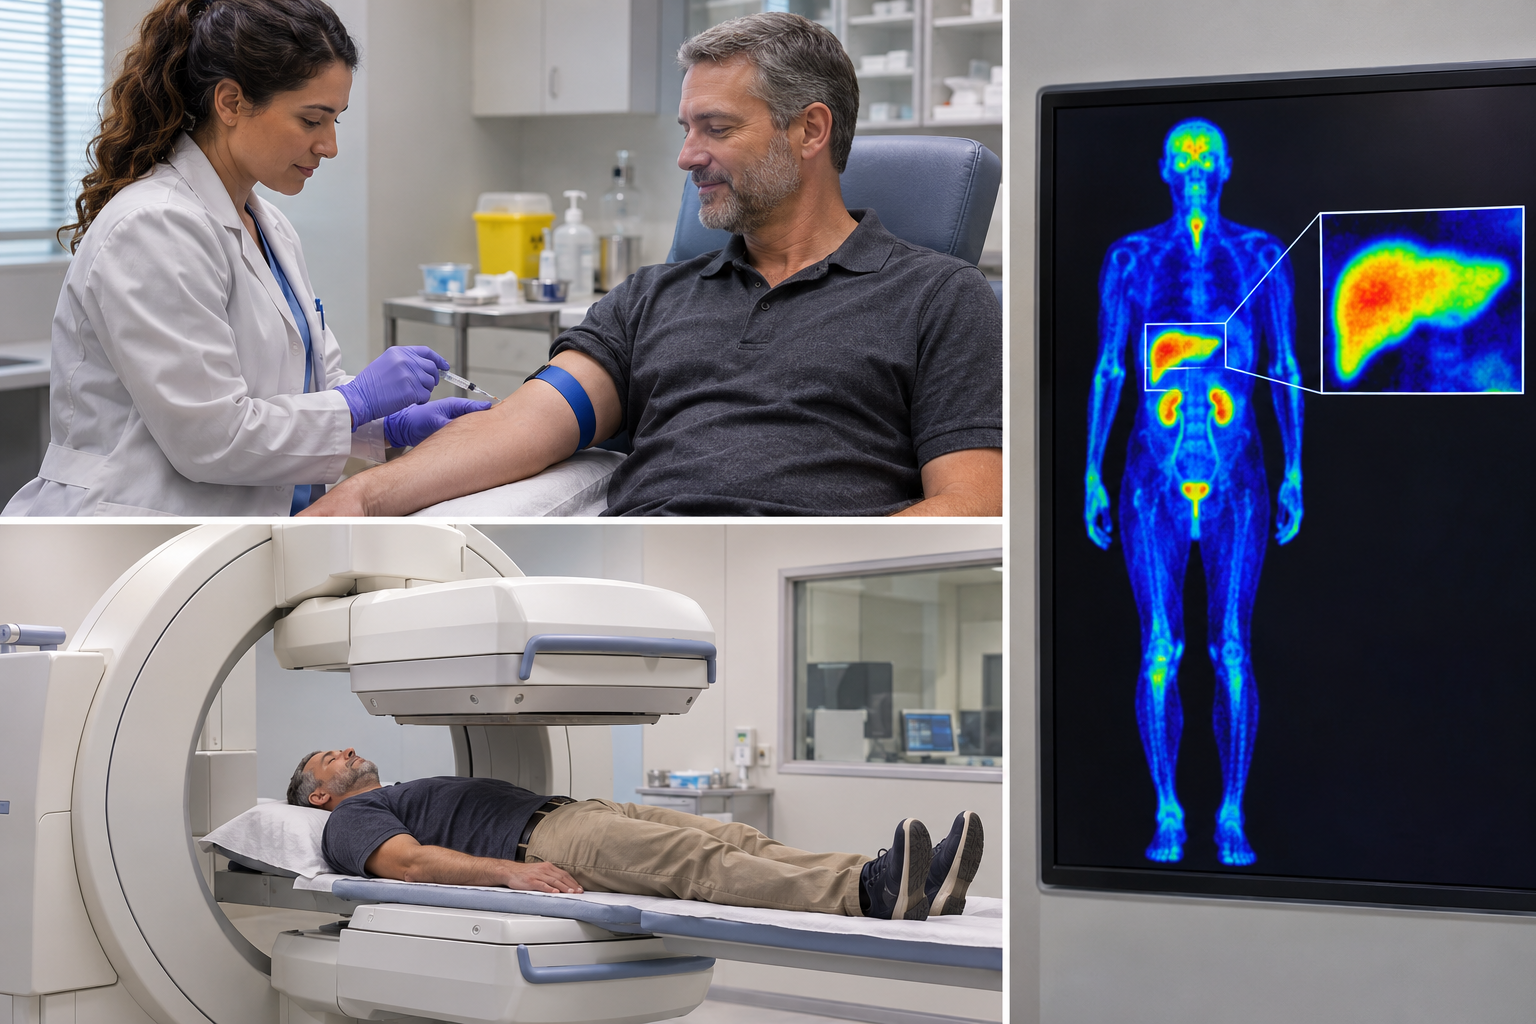
\includegraphics[width=\textwidth,keepaspectratio]{modalities/infographics/nuclear_medicine_realistic.png}
\end{center}
\begin{center}\footnotesize Radiopharmaceutical distribution reflects a tracer-specific biological process, and a gamma camera detects emitted photons to map that activity. AI-generated illustration; scan panel is not a patient study.\end{center}

\section{Overview}
Nuclear medicine is a diagnostic imaging discipline that uses radiopharmaceuticals to investigate physiological function, metabolism, tissue perfusion, receptor expression, and molecular processes within the human body.

Unlike CT and conventional MRI, which primarily visualize anatomical structures, nuclear medicine can reveal functional and molecular abnormalities before substantial anatomical changes become apparent.

Principal diagnostic modalities include planar scintigraphy, single-photon emission computed tomography (SPECT), positron emission tomography (PET), hybrid SPECT/CT, hybrid PET/CT, and hybrid PET/MRI. This chapter covers diseases and conditions for which nuclear medicine provides established or supplementary diagnostic information. Therapeutic nuclear medicine is excluded.

The 195 entries form a preliminary catalogue of nuclear medicine applications, including diagnosis, staging, localization, functional assessment, and treatment monitoring. Some entries overlap or represent historical or nonroutine applications; individual indications and radiopharmaceutical assignments require validation against clinical guidelines.

\section{Where nuclear medicine is used}
The following catalogue groups applications by disease category. Findings should be interpreted in the context of the administered radiopharmaceutical, acquisition protocol, and clinical question.

\subsection{Neurological and neurodegenerative diseases}
\begin{enumerate}[leftmargin=*,itemsep=0.45em,topsep=0.4em]
\item \textbf{Alzheimer disease.} Useful imaging findings include: Temporoparietal and posterior cingulate hypometabolism. Radiopharmaceutical: ¹⁸F-FDG.
\item \textbf{Alzheimer-associated amyloid pathology.} Useful imaging findings include: Increased cortical amyloid tracer retention. Radiopharmaceutical: ¹⁸F-Florbetapir, ¹⁸F-Flutemetamol.
\item \textbf{Alzheimer-associated tau pathology.} Useful imaging findings include: Increased regional tau tracer retention. Radiopharmaceutical: ¹⁸F-Flortaucipir.
\item \textbf{Cerebral circulatory arrest.} Useful imaging findings include: Absence of intracranial perfusion on a protocol-based ancillary study. Radiopharmaceutical: ⁹⁹ᵐTc-HMPAO.
\item \textbf{Cerebral ischemia.} Useful imaging findings include: Regional reduction in cerebral perfusion. Radiopharmaceutical: ⁹⁹ᵐTc-ECD.
\item \textbf{Corticobasal syndrome.} Useful imaging findings include: Asymmetric cortical and subcortical hypometabolism. Radiopharmaceutical: ¹⁸F-FDG.
\item \textbf{Dementia with Lewy bodies.} Useful imaging findings include: Occipital hypometabolism. Radiopharmaceutical: ¹⁸F-FDG.
\item \textbf{Focal epilepsy.} Useful imaging findings include: Increased ictal regional perfusion. Radiopharmaceutical: ⁹⁹ᵐTc-HMPAO.
\item \textbf{Frontotemporal dementia.} Useful imaging findings include: Frontal and anterior temporal hypometabolism. Radiopharmaceutical: ¹⁸F-FDG.
\item \textbf{Huntington disease.} Useful imaging findings include: Striatal hypometabolism. Radiopharmaceutical: ¹⁸F-FDG.
\item \textbf{Multiple system atrophy.} Useful imaging findings include: Reduced striatal dopamine transporter binding. Radiopharmaceutical: ¹²³I-Ioflupane.
\item \textbf{Parkinson disease.} Useful imaging findings include: Reduced striatal dopamine transporter binding. Radiopharmaceutical: ¹²³I-Ioflupane.
\item \textbf{Progressive supranuclear palsy.} Useful imaging findings include: Frontal and midbrain hypometabolism. Radiopharmaceutical: ¹⁸F-FDG.
\item \textbf{Temporal lobe epilepsy.} Useful imaging findings include: Interictal temporal hypometabolism. Radiopharmaceutical: ¹⁸F-FDG.
\item \textbf{Vascular dementia.} Useful imaging findings include: Regional metabolic or perfusion defects. Radiopharmaceutical: ¹⁸F-FDG.
\end{enumerate}
Dopamine transporter imaging cannot reliably distinguish Parkinson disease from several atypical degenerative parkinsonian syndromes.
In suspected death by neurologic criteria, radionuclide cerebral perfusion imaging is an ancillary test performed under applicable protocols; absent intracranial perfusion does not by itself establish the clinical diagnosis.

\subsection{Brain tumors}
\begin{enumerate}[leftmargin=*,itemsep=0.45em,topsep=0.4em]
\item \textbf{Astrocytoma.} Useful imaging findings include: Variable amino acid uptake. Radiopharmaceutical: ¹⁸F-FET.
\item \textbf{Brain metastases.} Useful imaging findings include: Variable amino acid tracer uptake. Radiopharmaceutical: ¹⁸F-FET.
\item \textbf{Glioblastoma.} Useful imaging findings include: Increased amino acid tracer uptake. Radiopharmaceutical: ¹⁸F-FET.
\item \textbf{Meningioma.} Useful imaging findings include: Increased somatostatin receptor expression. Radiopharmaceutical: ⁶⁸Ga-DOTATATE.
\item \textbf{Oligodendroglioma.} Useful imaging findings include: Variable or increased amino acid uptake. Radiopharmaceutical: ¹¹C-Methionine.
\item \textbf{Primary CNS lymphoma.} Useful imaging findings include: Markedly increased glucose metabolism. Radiopharmaceutical: ¹⁸F-FDG.
\item \textbf{Radiation necrosis.} Useful imaging findings include: Generally lower amino acid uptake than recurrent tumor, with overlap. Radiopharmaceutical: ¹⁸F-FET.
\item \textbf{Recurrent glioma.} Useful imaging findings include: Increased uptake within viable tumor tissue. Radiopharmaceutical: ¹⁸F-FET.
\end{enumerate}

\subsection{Cardiovascular diseases}
\begin{enumerate}[leftmargin=*,itemsep=0.45em,topsep=0.4em]
\item \textbf{Aortitis.} Useful imaging findings include: Increased aortic wall uptake. Radiopharmaceutical: ¹⁸F-FDG.
\item \textbf{Cardiac device infection.} Useful imaging findings include: Increased uptake surrounding implanted devices. Radiopharmaceutical: ¹⁸F-FDG.
\item \textbf{Cardiac sarcoidosis.} Useful imaging findings include: Focal myocardial inflammatory uptake. Radiopharmaceutical: ¹⁸F-FDG.
\item \textbf{Coronary artery disease.} Useful imaging findings include: Stress-induced myocardial perfusion defects. Radiopharmaceutical: ⁹⁹ᵐTc-Sestamibi.
\item \textbf{Coronary microvascular dysfunction.} Useful imaging findings include: Reduced myocardial flow reserve. Radiopharmaceutical: ⁸²Rb, ¹³N-Ammonia.
\item \textbf{Dilated cardiomyopathy.} Useful imaging findings include: Reduced ventricular ejection fraction; chamber size requires anatomical imaging correlation. Radiopharmaceutical: ⁹⁹ᵐTc-labeled RBCs (equilibrium radionuclide ventriculography).
\item \textbf{Giant cell arteritis.} Useful imaging findings include: Increased arterial wall metabolic activity. Radiopharmaceutical: ¹⁸F-FDG.
\item \textbf{Hibernating myocardium.} Useful imaging findings include: Reduced perfusion with preserved glucose metabolism (perfusion--metabolism mismatch). Radiopharmaceutical: ¹⁸F-FDG with paired perfusion imaging (e.g., ⁸²Rb or ¹³N-ammonia PET).
\item \textbf{Ischemic cardiomyopathy.} Useful imaging findings include: Regional perfusion and functional abnormalities. Radiopharmaceutical: ⁹⁹ᵐTc-Sestamibi.
\item \textbf{Myocardial ischemia.} Useful imaging findings include: Reversible myocardial perfusion defect. Radiopharmaceutical: ⁹⁹ᵐTc-Tetrofosmin.
\item \textbf{Previous myocardial infarction.} Useful imaging findings include: Fixed myocardial perfusion defect. Radiopharmaceutical: ⁹⁹ᵐTc-Sestamibi.
\item \textbf{Prosthetic valve endocarditis.} Useful imaging findings include: Abnormal periprosthetic tracer uptake. Radiopharmaceutical: ¹⁸F-FDG.
\item \textbf{Takayasu arteritis.} Useful imaging findings include: Increased uptake in inflamed large arteries. Radiopharmaceutical: ¹⁸F-FDG.
\item \textbf{Transthyretin cardiac amyloidosis.} Useful imaging findings include: Myocardial bone-tracer uptake assessed using validated visual and SPECT criteria. Radiopharmaceutical: ⁹⁹ᵐTc-PYP, DPD or HMDP.
\item \textbf{Vascular graft infection.} Useful imaging findings include: Abnormal uptake surrounding vascular grafts. Radiopharmaceutical: ¹⁸F-FDG.
\end{enumerate}
Bone-tracer uptake supports ATTR cardiac amyloidosis only in the appropriate clinical context. Evaluation for a monoclonal protein is required to avoid misclassifying AL amyloidosis; uptake alone is not diagnostic.

\subsection{Pulmonary diseases}
\begin{enumerate}[leftmargin=*,itemsep=0.45em,topsep=0.4em]
\item \textbf{Acute pulmonary embolism.} Useful imaging findings include: Segmental ventilation--perfusion mismatch; perfusion-only imaging may be used in selected protocols. Radiopharmaceutical: ⁹⁹ᵐTc-MAA plus a ventilation agent (e.g., ⁹⁹ᵐTc-Technegas or aerosol).
\item \textbf{Bronchogenic carcinoma.} Useful imaging findings include: Increased tumor glucose metabolism. Radiopharmaceutical: ¹⁸F-FDG.
\item \textbf{Chronic obstructive pulmonary disease.} Useful imaging findings include: Heterogeneous ventilation and perfusion. Radiopharmaceutical: ⁹⁹ᵐTc-MAA, Technegas.
\item \textbf{Chronic thromboembolic pulmonary hypertension.} Useful imaging findings include: Persistent mismatched ventilation--perfusion defects. Radiopharmaceutical: ⁹⁹ᵐTc-MAA plus a ventilation agent (e.g., ⁹⁹ᵐTc-Technegas or aerosol).
\item \textbf{Malignant pleural mesothelioma.} Useful imaging findings include: Increased pleural metabolic activity. Radiopharmaceutical: ¹⁸F-FDG.
\item \textbf{Pulmonary emphysema.} Useful imaging findings include: Regional ventilation and perfusion abnormalities. Radiopharmaceutical: ⁹⁹ᵐTc-MAA.
\item \textbf{Pulmonary fibrosis (selected preoperative regional function assessment).} Useful imaging findings include: Regional perfusion contribution to lung function; this study does not diagnose pulmonary fibrosis. Radiopharmaceutical: ⁹⁹ᵐTc-MAA.
\item \textbf{Pulmonary metastases.} Useful imaging findings include: Variable focal metabolic uptake. Radiopharmaceutical: ¹⁸F-FDG.
\item \textbf{Pulmonary sarcoidosis.} Useful imaging findings include: Increased metabolic activity in active inflammatory lesions. Radiopharmaceutical: ¹⁸F-FDG.
\item \textbf{Right-to-left pulmonary shunt (including selected assessment in pulmonary arteriovenous malformation).} Useful imaging findings include: Extrapulmonary activity used to detect or quantify right-to-left shunting; does not localize a malformation. Radiopharmaceutical: ⁹⁹ᵐTc-MAA.
\end{enumerate}

\subsection{Thyroid and parathyroid diseases}
\begin{enumerate}[leftmargin=*,itemsep=0.45em,topsep=0.4em]
\item \textbf{Autonomous thyroid nodule.} Useful imaging findings include: Focal increased tracer uptake. Radiopharmaceutical: ¹²³I.
\item \textbf{Congenital thyroid dysgenesis.} Useful imaging findings include: Absent or ectopic thyroid uptake. Radiopharmaceutical: ⁹⁹ᵐTc-Pertechnetate.
\item \textbf{Ectopic parathyroid adenoma.} Useful imaging findings include: Focal uptake at an abnormal anatomical location. Radiopharmaceutical: ¹⁸F-Fluorocholine.
\item \textbf{Ectopic thyroid tissue.} Useful imaging findings include: Tracer uptake outside the normal thyroid location. Radiopharmaceutical: ⁹⁹ᵐTc-Pertechnetate.
\item \textbf{Follicular thyroid carcinoma.} Useful imaging findings include: Possible radioiodine-avid metastatic lesions. Radiopharmaceutical: ¹²³I, ¹³¹I.
\item \textbf{Graves disease.} Useful imaging findings include: Diffusely increased thyroid uptake. Radiopharmaceutical: ¹²³I, ⁹⁹ᵐTc-Pertechnetate.
\item \textbf{Hashimoto thyroiditis.} Useful imaging findings include: Variable or heterogeneous uptake. Radiopharmaceutical: ¹²³I.
\item \textbf{Painless thyroiditis.} Useful imaging findings include: Reduced thyroid uptake. Radiopharmaceutical: ¹²³I.
\item \textbf{Papillary thyroid carcinoma.} Useful imaging findings include: Possible radioiodine uptake in residual or metastatic disease. Radiopharmaceutical: ¹²³I, ¹³¹I.
\item \textbf{Parathyroid adenoma.} Useful imaging findings include: Persistent focal tracer retention. Radiopharmaceutical: ⁹⁹ᵐTc-Sestamibi.
\item \textbf{Parathyroid hyperplasia.} Useful imaging findings include: Uptake in multiple enlarged glands. Radiopharmaceutical: ⁹⁹ᵐTc-Sestamibi.
\item \textbf{Radioiodine-refractory thyroid carcinoma.} Useful imaging findings include: Increased glucose metabolism in some lesions. Radiopharmaceutical: ¹⁸F-FDG.
\item \textbf{Subacute thyroiditis.} Useful imaging findings include: Markedly reduced thyroid uptake. Radiopharmaceutical: ¹²³I.
\item \textbf{Toxic multinodular goiter.} Useful imaging findings include: Heterogeneous increased thyroid uptake. Radiopharmaceutical: ¹²³I.
\item \textbf{Toxic thyroid adenoma.} Useful imaging findings include: Focal increased uptake with suppressed surrounding tissue. Radiopharmaceutical: ⁹⁹ᵐTc-Pertechnetate.
\end{enumerate}

\subsection{Bones and skeletal diseases}
\begin{enumerate}[leftmargin=*,itemsep=0.45em,topsep=0.4em]
\item \textbf{Acute osteomyelitis.} Useful imaging findings include: Increased perfusion, blood-pool and delayed uptake. Radiopharmaceutical: ⁹⁹ᵐTc-MDP.
\item \textbf{Breast cancer bone metastases.} Useful imaging findings include: Increased skeletal uptake or metabolism. Radiopharmaceutical: ⁹⁹ᵐTc-MDP, ¹⁸F-FDG.
\item \textbf{Chondrosarcoma.} Useful imaging findings include: Variable metabolic uptake. Radiopharmaceutical: ¹⁸F-FDG.
\item \textbf{Chronic osteomyelitis.} Useful imaging findings include: Abnormal osseous metabolic or inflammatory uptake. Radiopharmaceutical: ¹⁸F-FDG.
\item \textbf{Complex regional pain syndrome.} Useful imaging findings include: Variable regional periarticular uptake. Radiopharmaceutical: ⁹⁹ᵐTc-MDP.
\item \textbf{Ewing sarcoma.} Useful imaging findings include: Increased tumor glucose metabolism. Radiopharmaceutical: ¹⁸F-FDG.
\item \textbf{Fibrous dysplasia.} Useful imaging findings include: Increased regional skeletal uptake. Radiopharmaceutical: ⁹⁹ᵐTc-MDP.
\item \textbf{Heterotopic ossification.} Useful imaging findings include: Increased extraosseous bone-tracer uptake. Radiopharmaceutical: ⁹⁹ᵐTc-MDP.
\item \textbf{Hypertrophic osteoarthropathy.} Useful imaging findings include: Symmetric linear periosteal uptake. Radiopharmaceutical: ⁹⁹ᵐTc-MDP.
\item \textbf{Multiple myeloma.} Useful imaging findings include: Metabolically active marrow or skeletal lesions. Radiopharmaceutical: ¹⁸F-FDG.
\item \textbf{Occult fracture.} Useful imaging findings include: Increased uptake at fracture site. Radiopharmaceutical: ⁹⁹ᵐTc-MDP.
\item \textbf{Osteoblastic bone metastases.} Useful imaging findings include: Multifocal increased skeletal uptake. Radiopharmaceutical: ⁹⁹ᵐTc-MDP.
\item \textbf{Osteoblastoma.} Useful imaging findings include: Increased focal skeletal uptake. Radiopharmaceutical: ⁹⁹ᵐTc-MDP.
\item \textbf{Osteoid osteoma.} Useful imaging findings include: Intense focal uptake. Radiopharmaceutical: ⁹⁹ᵐTc-MDP.
\item \textbf{Osteonecrosis.} Useful imaging findings include: Reduced early perfusion or variable reparative uptake. Radiopharmaceutical: ⁹⁹ᵐTc-MDP.
\item \textbf{Osteosarcoma.} Useful imaging findings include: Increased tumor metabolic activity. Radiopharmaceutical: ¹⁸F-FDG.
\item \textbf{Paget disease of bone.} Useful imaging findings include: Intense uptake involving affected bone. Radiopharmaceutical: ⁹⁹ᵐTc-MDP.
\item \textbf{Prostate cancer bone metastases.} Useful imaging findings include: Increased osteoblastic activity. Radiopharmaceutical: ⁹⁹ᵐTc-MDP, ¹⁸F-NaF.
\item \textbf{Stress fracture.} Useful imaging findings include: Focal increased skeletal uptake. Radiopharmaceutical: ⁹⁹ᵐTc-MDP.
\item \textbf{Vertebral compression fracture.} Useful imaging findings include: Increased uptake in metabolically active fractures. Radiopharmaceutical: ⁹⁹ᵐTc-MDP.
\end{enumerate}
Conventional bone scintigraphy is less sensitive for purely osteolytic lesions, including many multiple myeloma lesions.

\subsection{Joint and prosthetic disorders}
\begin{enumerate}[leftmargin=*,itemsep=0.45em,topsep=0.4em]
\item \textbf{Aseptic prosthetic loosening.} Useful imaging findings include: Increased bone turnover at prosthetic interfaces. Radiopharmaceutical: ⁹⁹ᵐTc-MDP.
\item \textbf{Osteoarthritis.} Useful imaging findings include: Increased periarticular bone turnover. Radiopharmaceutical: ⁹⁹ᵐTc-MDP.
\item \textbf{Painful hip arthroplasty.} Useful imaging findings include: Abnormal periprosthetic tracer uptake. Radiopharmaceutical: ⁹⁹ᵐTc-MDP.
\item \textbf{Painful knee arthroplasty.} Useful imaging findings include: Abnormal regional bone turnover. Radiopharmaceutical: ⁹⁹ᵐTc-MDP.
\item \textbf{Prosthetic joint infection.} Useful imaging findings include: Abnormal periprosthetic leukocyte accumulation, interpreted with the clinical context and complementary imaging when indicated. Radiopharmaceutical: ¹¹¹In-Oxine leukocytes.
\item \textbf{Rheumatoid arthritis.} Useful imaging findings include: Increased inflammatory joint uptake. Radiopharmaceutical: ¹⁸F-FDG.
\item \textbf{Sacroiliac inflammation.} Useful imaging findings include: Variable increased metabolic activity. Radiopharmaceutical: ¹⁸F-FDG.
\item \textbf{Septic arthritis.} Useful imaging findings include: Increased inflammatory tracer accumulation. Radiopharmaceutical: ¹⁸F-FDG, labeled leukocytes.
\end{enumerate}

\subsection{Liver and biliary diseases}
\begin{enumerate}[leftmargin=*,itemsep=0.45em,topsep=0.4em]
\item \textbf{Acute cholecystitis.} Useful imaging findings include: Nonvisualization of the gallbladder under appropriate protocol. Radiopharmaceutical: ⁹⁹ᵐTc-Mebrofenin.
\item \textbf{Bile leak.} Useful imaging findings include: Extraluminal accumulation of biliary tracer. Radiopharmaceutical: ⁹⁹ᵐTc-Mebrofenin.
\item \textbf{Biliary atresia.} Useful imaging findings include: Absent intestinal tracer excretion after an appropriate protocol; this is not specific and may also occur with severe hepatocellular dysfunction. Radiopharmaceutical: ⁹⁹ᵐTc-Mebrofenin.
\item \textbf{Biliary obstruction.} Useful imaging findings include: Delayed or absent tracer passage into the intestine. Radiopharmaceutical: ⁹⁹ᵐTc-Mebrofenin.
\item \textbf{Cholangiocarcinoma.} Useful imaging findings include: Increased metabolic uptake in many tumors. Radiopharmaceutical: ¹⁸F-FDG.
\item \textbf{Chronic cholecystitis.} Useful imaging findings include: Delayed gallbladder visualization or abnormal emptying. Radiopharmaceutical: ⁹⁹ᵐTc-Disofenin.
\item \textbf{Focal nodular hyperplasia.} Useful imaging findings include: Preserved or increased reticuloendothelial tracer uptake in some lesions. Radiopharmaceutical: ⁹⁹ᵐTc-Sulfur colloid.
\item \textbf{Functional gallbladder disorder.} Useful imaging findings include: Reduced gallbladder ejection fraction. Radiopharmaceutical: ⁹⁹ᵐTc-Mebrofenin.
\item \textbf{Hepatic hemangioma.} Useful imaging findings include: Delayed blood-pool accumulation. Radiopharmaceutical: ⁹⁹ᵐTc-labeled RBCs.
\item \textbf{Hepatic metastases.} Useful imaging findings include: Focal abnormal metabolic or receptor-specific uptake. Radiopharmaceutical: ¹⁸F-FDG, ⁶⁸Ga-DOTATATE.
\item \textbf{Hepatocellular carcinoma.} Useful imaging findings include: Variable glucose metabolism. Radiopharmaceutical: ¹⁸F-FDG.
\item \textbf{Neonatal hepatitis.} Useful imaging findings include: Impaired hepatic uptake and excretion. Radiopharmaceutical: ⁹⁹ᵐTc-Mebrofenin.
\end{enumerate}

\subsection{Gastrointestinal diseases}
\begin{enumerate}[leftmargin=*,itemsep=0.45em,topsep=0.4em]
\item \textbf{Active gastrointestinal bleeding.} Useful imaging findings include: Extravascular accumulation and movement of labeled blood. Radiopharmaceutical: ⁹⁹ᵐTc-labeled RBCs.
\item \textbf{Chronic intestinal dysmotility.} Useful imaging findings include: Abnormal gastrointestinal transit. Radiopharmaceutical: Radiolabeled meals.
\item \textbf{Colonic slow-transit constipation.} Useful imaging findings include: Delayed colonic tracer progression. Radiopharmaceutical: ¹¹¹In-labeled tracer.
\item \textbf{Crohn disease.} Useful imaging findings include: Increased inflammatory bowel uptake. Radiopharmaceutical: ¹⁸F-FDG.
\item \textbf{Esophageal motility disorder.} Useful imaging findings include: Delayed esophageal tracer transit. Radiopharmaceutical: ⁹⁹ᵐTc-labeled liquid.
\item \textbf{Gastroparesis.} Useful imaging findings include: Delayed gastric emptying. Radiopharmaceutical: ⁹⁹ᵐTc-Sulfur colloid-labeled meal.
\item \textbf{Meckel diverticulum.} Useful imaging findings include: Ectopic gastric mucosal tracer uptake. Radiopharmaceutical: ⁹⁹ᵐTc-Pertechnetate.
\item \textbf{Protein-losing enteropathy.} Useful imaging findings include: Abnormal leakage of labeled protein into the bowel. Radiopharmaceutical: ⁹⁹ᵐTc-Human serum albumin.
\item \textbf{Rapid gastric emptying.} Useful imaging findings include: Accelerated gastric tracer clearance. Radiopharmaceutical: ⁹⁹ᵐTc-Sulfur colloid-labeled meal.
\item \textbf{Ulcerative colitis.} Useful imaging findings include: Increased colonic inflammatory uptake. Radiopharmaceutical: ¹⁸F-FDG.
\end{enumerate}

\subsection{Renal and urinary tract diseases}
\begin{enumerate}[leftmargin=*,itemsep=0.45em,topsep=0.4em]
\item \textbf{Acute pyelonephritis.} Useful imaging findings include: Focal renal cortical uptake defects. Radiopharmaceutical: ⁹⁹ᵐTc-DMSA.
\item \textbf{Ectopic kidney.} Useful imaging findings include: Renal tracer uptake at an abnormal location. Radiopharmaceutical: ⁹⁹ᵐTc-DMSA.
\item \textbf{Horseshoe kidney.} Useful imaging findings include: Abnormal renal configuration. Radiopharmaceutical: ⁹⁹ᵐTc-DMSA.
\item \textbf{Hydronephrosis.} Useful imaging findings include: Collecting-system retention with variable drainage. Radiopharmaceutical: ⁹⁹ᵐTc-MAG3.
\item \textbf{Obstructive uropathy.} Useful imaging findings include: Impaired urinary tracer clearance. Radiopharmaceutical: ⁹⁹ᵐTc-MAG3.
\item \textbf{Reflux nephropathy.} Useful imaging findings include: Cortical defects and impaired differential function. Radiopharmaceutical: ⁹⁹ᵐTc-DMSA.
\item \textbf{Renal artery stenosis.} Useful imaging findings include: Abnormal renal perfusion or captopril renographic response. Radiopharmaceutical: ⁹⁹ᵐTc-DTPA.
\item \textbf{Renal cortical scarring.} Useful imaging findings include: Persistent cortical tracer defects. Radiopharmaceutical: ⁹⁹ᵐTc-DMSA.
\item \textbf{Renal dysplasia.} Useful imaging findings include: Reduced or abnormal cortical tracer distribution. Radiopharmaceutical: ⁹⁹ᵐTc-DMSA.
\item \textbf{Renal infarction.} Useful imaging findings include: Regional absence of cortical uptake. Radiopharmaceutical: ⁹⁹ᵐTc-DMSA.
\item \textbf{Renal transplant dysfunction.} Useful imaging findings include: Abnormal perfusion, uptake or excretion. Radiopharmaceutical: ⁹⁹ᵐTc-MAG3.
\item \textbf{Renal transplant urinary leak.} Useful imaging findings include: Extraluminal urinary tracer accumulation. Radiopharmaceutical: ⁹⁹ᵐTc-MAG3.
\item \textbf{Renovascular hypertension.} Useful imaging findings include: Altered renal function following ACE inhibition. Radiopharmaceutical: ⁹⁹ᵐTc-MAG3.
\item \textbf{Ureteropelvic junction obstruction.} Useful imaging findings include: Delayed tracer drainage despite diuretic administration. Radiopharmaceutical: ⁹⁹ᵐTc-MAG3.
\item \textbf{Vesicoureteral reflux.} Useful imaging findings include: Retrograde tracer movement into ureters. Radiopharmaceutical: Radionuclide cystography tracer.
\end{enumerate}

\subsection{Neuroendocrine and adrenal diseases}
\begin{enumerate}[leftmargin=*,itemsep=0.45em,topsep=0.4em]
\item \textbf{Adrenocortical carcinoma.} Useful imaging findings include: Increased glucose metabolism in many tumors. Radiopharmaceutical: ¹⁸F-FDG.
\item \textbf{Bronchial carcinoid.} Useful imaging findings include: Increased somatostatin receptor expression. Radiopharmaceutical: ⁶⁸Ga-DOTATATE.
\item \textbf{Gastrinoma.} Useful imaging findings include: Increased somatostatin receptor uptake. Radiopharmaceutical: ⁶⁸Ga-DOTATATE.
\item \textbf{Gastroenteropancreatic neuroendocrine tumor.} Useful imaging findings include: Increased somatostatin receptor tracer uptake. Radiopharmaceutical: ⁶⁸Ga-DOTATATE.
\item \textbf{Insulinoma.} Useful imaging findings include: Variable GLP-1 receptor or somatostatin receptor uptake. Radiopharmaceutical: Radiolabeled exendin.
\item \textbf{Medullary thyroid carcinoma.} Useful imaging findings include: Variable amino acid or receptor-specific uptake. Radiopharmaceutical: ¹⁸F-FDOPA.
\item \textbf{Merkel cell carcinoma.} Useful imaging findings include: Increased glucose metabolism. Radiopharmaceutical: ¹⁸F-FDG.
\item \textbf{Neuroblastoma.} Useful imaging findings include: Increased norepinephrine transporter-related uptake. Radiopharmaceutical: ¹²³I-MIBG.
\item \textbf{Pancreatic neuroendocrine tumor.} Useful imaging findings include: Increased receptor-specific uptake. Radiopharmaceutical: ⁶⁸Ga-DOTATATE.
\item \textbf{Paraganglioma.} Useful imaging findings include: Increased somatostatin receptor expression. Radiopharmaceutical: ⁶⁸Ga-DOTATATE.
\item \textbf{Pheochromocytoma.} Useful imaging findings include: Increased catecholamine-related or receptor-specific uptake. Radiopharmaceutical: ¹²³I-MIBG, ⁶⁸Ga-DOTATATE.
\item \textbf{Small bowel neuroendocrine tumor.} Useful imaging findings include: Receptor-positive primary and metastatic lesions. Radiopharmaceutical: ⁶⁸Ga-DOTATATE.
\end{enumerate}

\subsection{Hematological malignancies}
\begin{enumerate}[leftmargin=*,itemsep=0.45em,topsep=0.4em]
\item \textbf{Burkitt lymphoma.} Useful imaging findings include: Intense metabolic uptake. Radiopharmaceutical: ¹⁸F-FDG.
\item \textbf{Diffuse large B-cell lymphoma.} Useful imaging findings include: Markedly increased metabolic activity. Radiopharmaceutical: ¹⁸F-FDG.
\item \textbf{Extramedullary plasmacytoma.} Useful imaging findings include: Hypermetabolic soft-tissue lesion. Radiopharmaceutical: ¹⁸F-FDG.
\item \textbf{Follicular lymphoma.} Useful imaging findings include: Increased nodal metabolic activity. Radiopharmaceutical: ¹⁸F-FDG.
\item \textbf{Hodgkin lymphoma.} Useful imaging findings include: Hypermetabolic lymph nodes and extranodal lesions. Radiopharmaceutical: ¹⁸F-FDG.
\item \textbf{Mantle cell lymphoma.} Useful imaging findings include: Variable or increased metabolic uptake. Radiopharmaceutical: ¹⁸F-FDG.
\item \textbf{Marginal zone lymphoma.} Useful imaging findings include: Variable metabolic activity. Radiopharmaceutical: ¹⁸F-FDG.
\item \textbf{Multiple myeloma.} Useful imaging findings include: Focal or diffuse metabolically active marrow lesions. Radiopharmaceutical: ¹⁸F-FDG.
\item \textbf{Peripheral T-cell lymphoma.} Useful imaging findings include: Increased metabolic uptake. Radiopharmaceutical: ¹⁸F-FDG.
\item \textbf{Primary mediastinal B-cell lymphoma.} Useful imaging findings include: Increased mediastinal metabolic activity. Radiopharmaceutical: ¹⁸F-FDG.
\item \textbf{Richter transformation.} Useful imaging findings include: Increased metabolic activity in suspicious lesions. Radiopharmaceutical: ¹⁸F-FDG.
\item \textbf{Solitary plasmacytoma.} Useful imaging findings include: Focal metabolically active lesion. Radiopharmaceutical: ¹⁸F-FDG.
\end{enumerate}

\subsection{Solid malignant tumors}
Nuclear medicine is extensively used in oncology for tumor staging, treatment response assessment, recurrence detection, and selection of targeted therapies.
\begin{enumerate}[leftmargin=*,itemsep=0.45em,topsep=0.4em]
\item \textbf{Bladder carcinoma.} Useful imaging findings include: Increased tumor or metastatic metabolic activity. Radiopharmaceutical: ¹⁸F-FDG.
\item \textbf{Breast carcinoma.} Useful imaging findings include: Variable increased tumor metabolism. Radiopharmaceutical: ¹⁸F-FDG.
\item \textbf{Cancer of unknown primary.} Useful imaging findings include: Abnormal metabolic foci suggesting primary tumor. Radiopharmaceutical: ¹⁸F-FDG.
\item \textbf{Cervical carcinoma.} Useful imaging findings include: Increased primary and metastatic tumor uptake. Radiopharmaceutical: ¹⁸F-FDG.
\item \textbf{Colorectal carcinoma.} Useful imaging findings include: Increased metabolic activity. Radiopharmaceutical: ¹⁸F-FDG.
\item \textbf{Endometrial carcinoma.} Useful imaging findings include: Hypermetabolic uterine or metastatic lesions. Radiopharmaceutical: ¹⁸F-FDG.
\item \textbf{Esophageal carcinoma.} Useful imaging findings include: Hypermetabolic esophageal lesion. Radiopharmaceutical: ¹⁸F-FDG.
\item \textbf{Estrogen receptor-positive breast carcinoma.} Useful imaging findings include: Increased estrogen receptor tracer binding. Radiopharmaceutical: ¹⁸F-FES.
\item \textbf{Gastric carcinoma.} Useful imaging findings include: Variable metabolic activity. Radiopharmaceutical: ¹⁸F-FDG.
\item \textbf{Head and neck squamous cell carcinoma.} Useful imaging findings include: Increased tumor metabolic activity. Radiopharmaceutical: ¹⁸F-FDG.
\item \textbf{Laryngeal carcinoma.} Useful imaging findings include: Increased metabolic activity. Radiopharmaceutical: ¹⁸F-FDG.
\item \textbf{Malignant melanoma.} Useful imaging findings include: Hypermetabolic primary or metastatic lesions. Radiopharmaceutical: ¹⁸F-FDG.
\item \textbf{Nasopharyngeal carcinoma.} Useful imaging findings include: Increased metabolic activity. Radiopharmaceutical: ¹⁸F-FDG.
\item \textbf{Non-small cell lung carcinoma.} Useful imaging findings include: Increased tumor glucose metabolism. Radiopharmaceutical: ¹⁸F-FDG.
\item \textbf{Oral squamous cell carcinoma.} Useful imaging findings include: Increased metabolic activity. Radiopharmaceutical: ¹⁸F-FDG.
\item \textbf{Ovarian carcinoma.} Useful imaging findings include: Hypermetabolic pelvic and peritoneal lesions. Radiopharmaceutical: ¹⁸F-FDG.
\item \textbf{Pancreatic adenocarcinoma.} Useful imaging findings include: Increased tumor metabolism in many cases. Radiopharmaceutical: ¹⁸F-FDG.
\item \textbf{Prostate adenocarcinoma.} Useful imaging findings include: Increased PSMA-targeted tracer uptake. Radiopharmaceutical: ⁶⁸Ga-PSMA-11.
\item \textbf{Recurrent prostate carcinoma.} Useful imaging findings include: PSMA-positive recurrent or metastatic lesions. Radiopharmaceutical: ¹⁸F-DCFPyL.
\item \textbf{Renal cell carcinoma.} Useful imaging findings include: Variable metabolic uptake in metastatic lesions. Radiopharmaceutical: ¹⁸F-FDG.
\item \textbf{Rhabdomyosarcoma.} Useful imaging findings include: Metabolically active tumor lesions. Radiopharmaceutical: ¹⁸F-FDG.
\item \textbf{Small cell lung carcinoma.} Useful imaging findings include: Hypermetabolic primary and metastatic lesions. Radiopharmaceutical: ¹⁸F-FDG.
\item \textbf{Soft-tissue sarcoma.} Useful imaging findings include: Variable increased tumor metabolism. Radiopharmaceutical: ¹⁸F-FDG.
\item \textbf{Testicular seminoma.} Useful imaging findings include: Increased uptake in viable residual tumor. Radiopharmaceutical: ¹⁸F-FDG.
\end{enumerate}

\subsection{Infectious and inflammatory diseases}
\begin{enumerate}[leftmargin=*,itemsep=0.45em,topsep=0.4em]
\item \textbf{Diabetic foot osteomyelitis.} Useful imaging findings include: Abnormal osseous leukocyte accumulation. Radiopharmaceutical: ⁹⁹ᵐTc-HMPAO leukocytes.
\item \textbf{Fever of unknown origin.} Useful imaging findings include: Abnormal inflammatory or infectious metabolic foci. Radiopharmaceutical: ¹⁸F-FDG.
\item \textbf{IgG4-related disease.} Useful imaging findings include: Multiorgan inflammatory uptake. Radiopharmaceutical: ¹⁸F-FDG.
\item \textbf{Infected orthopedic hardware.} Useful imaging findings include: Abnormal peri-implant leukocyte uptake. Radiopharmaceutical: Labeled leukocytes.
\item \textbf{Occult abscess.} Useful imaging findings include: Focal inflammatory tracer accumulation. Radiopharmaceutical: ¹⁸F-FDG.
\item \textbf{Polymyalgia rheumatica.} Useful imaging findings include: Characteristic periarticular inflammatory uptake. Radiopharmaceutical: ¹⁸F-FDG.
\item \textbf{Retroperitoneal fibrosis.} Useful imaging findings include: Increased metabolic activity in active inflammatory tissue. Radiopharmaceutical: ¹⁸F-FDG.
\item \textbf{Spondylodiscitis.} Useful imaging findings include: Increased uptake involving disc and adjacent vertebrae. Radiopharmaceutical: ¹⁸F-FDG.
\item \textbf{Systemic sarcoidosis.} Useful imaging findings include: Hypermetabolic granulomatous lesions. Radiopharmaceutical: ¹⁸F-FDG.
\item \textbf{Tuberculosis.} Useful imaging findings include: Increased metabolic activity in active lesions. Radiopharmaceutical: ¹⁸F-FDG.
\item \textbf{Vascular prosthesis infection.} Useful imaging findings include: Abnormal graft-associated tracer accumulation. Radiopharmaceutical: ¹⁸F-FDG.
\item \textbf{Vertebral osteomyelitis.} Useful imaging findings include: Increased vertebral metabolic uptake. Radiopharmaceutical: ¹⁸F-FDG.
\end{enumerate}

\subsection{Lymphatic and splenic abnormalities}
\begin{enumerate}[leftmargin=*,itemsep=0.45em,topsep=0.4em]
\item \textbf{Accessory spleen.} Useful imaging findings include: Focal uptake corresponding to functioning splenic tissue. Radiopharmaceutical: ⁹⁹ᵐTc-Heat-damaged RBCs.
\item \textbf{Chylous leakage.} Useful imaging findings include: Abnormal lymphatic tracer accumulation. Radiopharmaceutical: ⁹⁹ᵐTc-Nanocolloid.
\item \textbf{Functional asplenia.} Useful imaging findings include: Markedly reduced splenic uptake. Radiopharmaceutical: ⁹⁹ᵐTc-Sulfur colloid.
\item \textbf{Lymphatic obstruction.} Useful imaging findings include: Interrupted lymphatic tracer progression. Radiopharmaceutical: ⁹⁹ᵐTc-Nanocolloid.
\item \textbf{Primary lymphedema.} Useful imaging findings include: Delayed or absent lymphatic drainage. Radiopharmaceutical: ⁹⁹ᵐTc-Nanocolloid.
\item \textbf{Secondary lymphedema.} Useful imaging findings include: Impaired lymphatic transport. Radiopharmaceutical: ⁹⁹ᵐTc-Nanocolloid.
\item \textbf{Splenosis.} Useful imaging findings include: Uptake within ectopic functioning splenic tissue. Radiopharmaceutical: ⁹⁹ᵐTc-Heat-damaged RBCs.
\end{enumerate}

\subsection{Summary of catalogue}
\begin{center}
\begin{tabular}{@{}p{0.70\textwidth}r@{}}
\toprule
\textbf{Disease category} & \textbf{Entries} \\
\midrule
Bones and skeletal diseases & 20 \\
Brain tumors & 8 \\
Cardiovascular diseases & 15 \\
Gastrointestinal diseases & 10 \\
Hematological malignancies & 12 \\
Infectious and inflammatory diseases & 12 \\
Joint and prosthetic disorders & 8 \\
Liver and biliary diseases & 12 \\
Lymphatic and splenic abnormalities & 7 \\
Neuroendocrine and adrenal diseases & 12 \\
Neurological and neurodegenerative diseases & 15 \\
Pulmonary diseases & 10 \\
Renal and urinary tract diseases & 15 \\
Solid malignant tumors & 24 \\
Thyroid and parathyroid diseases & 15 \\
Total & 195 \\
\bottomrule
\end{tabular}
\end{center}

\subsection{Major nuclear medicine imaging techniques}
\begin{longtable}{@{}p{0.38\textwidth}p{0.54\textwidth}@{}}
\toprule
\textbf{Imaging technique} & \textbf{Primary clinical application} \\
\midrule
\endfirsthead
\toprule
\textbf{Imaging technique} & \textbf{Primary clinical application} \\
\midrule
\endhead
Bone scintigraphy & Skeletal remodeling and osteoblastic activity \\
Dynamic scintigraphy & Temporal changes in tracer distribution \\
Gated SPECT & Myocardial perfusion and ventricular function \\
Hepatobiliary scintigraphy (HIDA) & Hepatobiliary function \\
Lymphoscintigraphy & Lymphatic drainage and sentinel node mapping \\
Myocardial perfusion imaging & Myocardial ischemia and perfusion \\
PET & Molecular and metabolic imaging \\
PET/CT & Metabolic and anatomical imaging \\
PET/MRI & Molecular imaging with superior soft-tissue characterization \\
Planar scintigraphy & Organ function and tracer distribution \\
Radioiodine whole-body scanning & Differentiated thyroid cancer assessment \\
Radionuclide ventriculography (MUGA) & Quantitative ventricular function \\
Renography & Renal perfusion, function and drainage \\
SPECT & Three-dimensional radiotracer distribution \\
SPECT/CT & Functional and anatomical localization \\
Ventilation-perfusion scintigraphy & Pulmonary ventilation and perfusion \\
Whole-body scintigraphy & Skeletal and systemic disease assessment \\
\bottomrule
\end{longtable}

\subsection{Major diagnostic radiopharmaceuticals}
\begin{longtable}{@{}p{0.27\textwidth}p{0.36\textwidth}p{0.29\textwidth}@{}}
\toprule
\textbf{Radiopharmaceutical} & \textbf{Biological process or molecular target} & \textbf{Primary application} \\
\midrule
\endfirsthead
\toprule
\textbf{Radiopharmaceutical} & \textbf{Biological process or molecular target} & \textbf{Primary application} \\
\midrule
\endhead
¹²³I-Ioflupane & Dopamine transporters & Parkinsonian syndromes \\
¹²³I-MIBG & Norepinephrine transport & Neuroendocrine tumors \\
¹²³I-Sodium iodide & Thyroid iodine transport & Thyroid imaging \\
¹³N-Ammonia & Myocardial perfusion & Cardiology \\
¹³¹I-Sodium iodide & Thyroid iodine transport & Differentiated thyroid cancer \\
¹¹C-Methionine & Amino acid transport & Brain tumors \\
¹¹¹In-Oxine leukocytes & Leukocyte migration & Infection imaging \\
¹⁵O-Water & Tissue perfusion & Quantitative perfusion imaging \\
¹⁸F-DCFPyL & PSMA expression & Prostate cancer \\
¹⁸F-FDG & Glucose metabolism & Oncology, infection, neurology \\
¹⁸F-FDOPA & Amino acid and dopamine-related metabolism & Neurology and neuroendocrine tumors \\
¹⁸F-FES & Estrogen receptors & Breast cancer \\
¹⁸F-FET & Amino acid transport & Brain tumors \\
¹⁸F-Florbetapir & Amyloid plaques & Alzheimer-associated pathology \\
¹⁸F-Flortaucipir & Aggregated tau & Alzheimer-associated pathology \\
¹⁸F-Fluorocholine & Choline metabolism & Parathyroid localization and oncology \\
¹⁸F-Flutemetamol & Amyloid plaques & Alzheimer-associated pathology \\
¹⁸F-NaF & Bone mineral turnover & Skeletal imaging \\
⁶⁷Ga-Citrate & Inflammatory and tumor-associated accumulation & Selected infection and tumor imaging \\
⁶⁸Ga-DOTATATE & Somatostatin receptors & Neuroendocrine tumors \\
⁶⁸Ga-DOTATOC & Somatostatin receptors & Neuroendocrine tumors \\
⁶⁸Ga-PSMA-11 & PSMA expression & Prostate cancer \\
⁸²Rb & Myocardial perfusion & Cardiology \\
⁹⁹ᵐTc-DMSA & Renal cortical retention & Renal cortical imaging \\
⁹⁹ᵐTc-DTPA & Glomerular filtration & Renal imaging \\
⁹⁹ᵐTc-ECD & Cerebral perfusion & Neurology \\
⁹⁹ᵐTc-HDP & Bone remodeling & Bone scintigraphy \\
⁹⁹ᵐTc-HMPAO & Cerebral perfusion or leukocyte labeling & Neurology and infection \\
⁹⁹ᵐTc-MAA & Pulmonary perfusion & Pulmonary embolism \\
⁹⁹ᵐTc-MAG3 & Renal tubular secretion & Renography \\
⁹⁹ᵐTc-MDP & Bone remodeling & Bone scintigraphy \\
⁹⁹ᵐTc-Mebrofenin & Hepatobiliary transport & Hepatobiliary imaging \\
⁹⁹ᵐTc-Pertechnetate & Anion transport & Thyroid and gastric mucosal imaging \\
⁹⁹ᵐTc-PYP & Bone-seeking tracer retention & Cardiac amyloidosis \\
⁹⁹ᵐTc-Sestamibi & Perfusion and mitochondrial retention & Cardiac and parathyroid imaging \\
⁹⁹ᵐTc-Sulfur colloid & Reticuloendothelial uptake or labeled meal transit & Hepatic and gastrointestinal imaging \\
⁹⁹ᵐTc-Tetrofosmin & Myocardial perfusion & Cardiology \\
\bottomrule
\end{longtable}

\subsection{Quantitative nuclear medicine parameters}
\begin{longtable}{@{}p{0.34\textwidth}p{0.16\textwidth}p{0.42\textwidth}@{}}
\toprule
\textbf{Parameter} & \textbf{Abbreviation} & \textbf{Clinical significance} \\
\midrule
\endfirsthead
\toprule
\textbf{Parameter} & \textbf{Abbreviation} & \textbf{Clinical significance} \\
\midrule
\endhead
Differential renal function & DRF & Relative contribution of each kidney \\
Gallbladder ejection fraction & GBEF & Gallbladder emptying function \\
Gastric retention percentage & --- & Gastric emptying assessment \\
Glomerular filtration rate & GFR & Renal filtration function \\
Injected activity & MBq & Administered radioactive activity \\
Lean body mass-normalized SUV & SUL & Uptake adjusted for lean body mass \\
Left ventricular ejection fraction & LVEF & Ventricular systolic function \\
Maximum standardized uptake value & SUVmax & Maximum voxel uptake within a lesion \\
Mean standardized uptake value & SUVmean & Average uptake within a defined region \\
Metabolic tumor volume & MTV & Volume of metabolically active tumor \\
Myocardial blood flow & MBF & Quantitative myocardial perfusion \\
Myocardial flow reserve & MFR & Stress-to-rest myocardial blood flow ratio \\
Peak standardized uptake value & SUVpeak & Uptake within a small highest-activity region \\
Radioactive iodine uptake & RAIU & Thyroid iodine uptake \\
Specific binding ratio & SBR & Dopamine transporter or receptor binding \\
Standardized uptake value & SUV & Normalized radiotracer accumulation \\
Target-to-background ratio & TBR & Relative target uptake \\
Total lesion glycolysis & TLG & Combined tumor volume and FDG uptake \\
Tumor-to-background ratio & TBR & Relative lesion uptake \\
\bottomrule
\end{longtable}

For example, a commonly used body weight-normalized PET standardized uptake value is:
\begin{equation}
SUV_{bw}=\frac{C_{\text{tissue}}\;(\mathrm{MBq/mL})}{A_{\text{injected}}\;(\mathrm{MBq})/W_{\text{body}}\;(\mathrm{g})}.
\end{equation}
Another commonly used oncological measurement is:
\begin{equation}
TLG=MTV\times SUV_{\text{mean}}.
\end{equation}
SUV measurements are affected by acquisition timing, blood glucose, reconstruction algorithms, scanner calibration, and partial-volume effects.

\subsection{Standardized reporting systems}
\begin{longtable}{@{}p{0.38\textwidth}p{0.54\textwidth}@{}}
\toprule
\textbf{Reporting system} & \textbf{Clinical application} \\
\midrule
\endfirsthead
\toprule
\textbf{Reporting system} & \textbf{Clinical application} \\
\midrule
\endhead
Centiloid scale & Standardized cerebral amyloid burden \\
Deauville five-point scale & Lymphoma treatment response \\
EORTC PET response criteria & Metabolic tumor response \\
Krenning score & Somatostatin receptor tracer uptake \\
Lugano classification & Lymphoma staging and response \\
PERCIST & Metabolic tumor response assessment \\
Perugini grading & Cardiac amyloidosis scintigraphy \\
PROMISE/miTNM & Molecular imaging staging of prostate cancer \\
PSMA-RADS & PSMA-targeted prostate cancer imaging \\
SSTR-RADS & Somatostatin receptor imaging \\
Summed difference score (SDS) & Reversible myocardial ischemia \\
Summed rest score (SRS) & Resting myocardial perfusion abnormalities \\
Summed stress score (SSS) & Myocardial perfusion abnormalities \\
V/Q interpretation criteria & Pulmonary embolism assessment \\
\bottomrule
\end{longtable}

\subsection{Published nuclear medicine imaging datasets and sources}
\begin{longtable}{@{}p{0.38\textwidth}p{0.54\textwidth}@{}}
\toprule
\textbf{Source} & \textbf{Primary utility} \\
\midrule
\endfirsthead
\toprule
\textbf{Source} & \textbf{Primary utility} \\
\midrule
\endhead
ADNI & Amyloid, tau and FDG brain PET \\
AutoPET Challenge & Whole-body PET/CT tumor segmentation \\
European Association of Nuclear Medicine & Clinical guidelines and imaging standards \\
International Atomic Energy Agency & Nuclear medicine education and technical standards \\
OpenNeuro & Selected neuroimaging and PET datasets \\
Parkinson's Progression Markers Initiative & Dopamine transporter imaging \\
PubMed Central & Published clinical images and studies \\
Radiopaedia & Annotated clinical nuclear medicine images \\
Society of Nuclear Medicine and Molecular Imaging & Clinical guidelines and protocols \\
The Cancer Imaging Archive (TCIA) & Oncological PET/CT datasets \\
\bottomrule
\end{longtable}

\subsection{Recommended metadata for a nuclear medicine dataset}
\begin{longtable}{@{}p{0.45\textwidth}p{0.49\textwidth}@{}}
\toprule
\textbf{Attribute} & \textbf{Example} \\
\midrule
Acquisition duration & 20 minutes \\
Administered activity & 150 MBq \\
Anatomical region & Whole body \\
Annotation & Segmentation mask \\
Attenuation correction & CT-based \\
Diagnostic reference standard & Histopathological confirmation \\
Disease & Prostate adenocarcinoma \\
Image format & DICOM \\
Image license & CC BY or other specified license \\
Image representation & Axial, coronal, sagittal, MIP \\
Imaging modality & PET/CT \\
Metabolic tumor volume & 15 cm$^3$ \\
Molecular target & Prostate-specific membrane antigen \\
Publication reference & DOI or PMID \\
Radiological finding & Increased focal PSMA tracer uptake \\
Radionuclide & Gallium-68 \\
Radiopharmaceutical & ⁶⁸Ga-PSMA-11 \\
Reconstruction algorithm & OSEM \\
SUVmax & 12.5 \\
Uptake period & 60 minutes \\
\bottomrule
\end{longtable}

\subsection{Interpreting radiopharmaceutical-dependent findings}
Interpretation depends fundamentally on the radiopharmaceutical administered.
\begin{longtable}{@{}p{0.36\textwidth}p{0.58\textwidth}@{}}
\toprule
\textbf{Modality} & \textbf{Primary information measured} \\
\midrule
\endfirsthead
\toprule
\textbf{Modality} & \textbf{Primary information measured} \\
\midrule
\endhead
CT & Tissue attenuation coefficients \\
Diffusion MRI & Apparent molecular diffusion \\
Doppler ultrasound & Motion and blood flow \\
Functional MRI & Hemodynamic responses \\
PET & Positron-emitting radiotracer distribution \\
SPECT & Gamma-emitting radiotracer distribution \\
Structural MRI & Magnetic resonance signal and relaxation properties \\
Ultrasound & Acoustic reflection \\
X-ray & X-ray attenuation \\
\bottomrule
\end{longtable}

For example, the same prostate cancer lesion may appear differently across nuclear medicine examinations:
\begin{longtable}{@{}p{0.32\textwidth}p{0.62\textwidth}@{}}
\toprule
\textbf{Radiopharmaceutical} & \textbf{Information obtained} \\
\midrule
\endfirsthead
\toprule
\textbf{Radiopharmaceutical} & \textbf{Information obtained} \\
\midrule
\endhead
¹⁸F-FDG & Glucose metabolism \\
¹⁸F-Fluorocholine & Choline metabolism \\
⁶⁸Ga-PSMA-11 & PSMA expression \\
⁹⁹ᵐTc-MDP & Associated osteoblastic activity in skeletal lesions \\
\bottomrule
\end{longtable}

For AI-based medical diagnosis, the radiopharmaceutical is a fundamental input parameter, not optional metadata. Increased uptake does not universally indicate malignancy, and reduced uptake does not universally indicate absence of disease.

The 195 entries are a preliminary catalogue of nuclear medicine applications. Some overlap, some represent historical or nonroutine applications, and individual indications and radiopharmaceutical assignments have not been independently validated against clinical guidelines.

\chapter{Single-Photon Emission Computed Tomography (SPECT)}
\label{ch:spect}

% Chapter-opening illustrated modality infographic.
\begin{center}
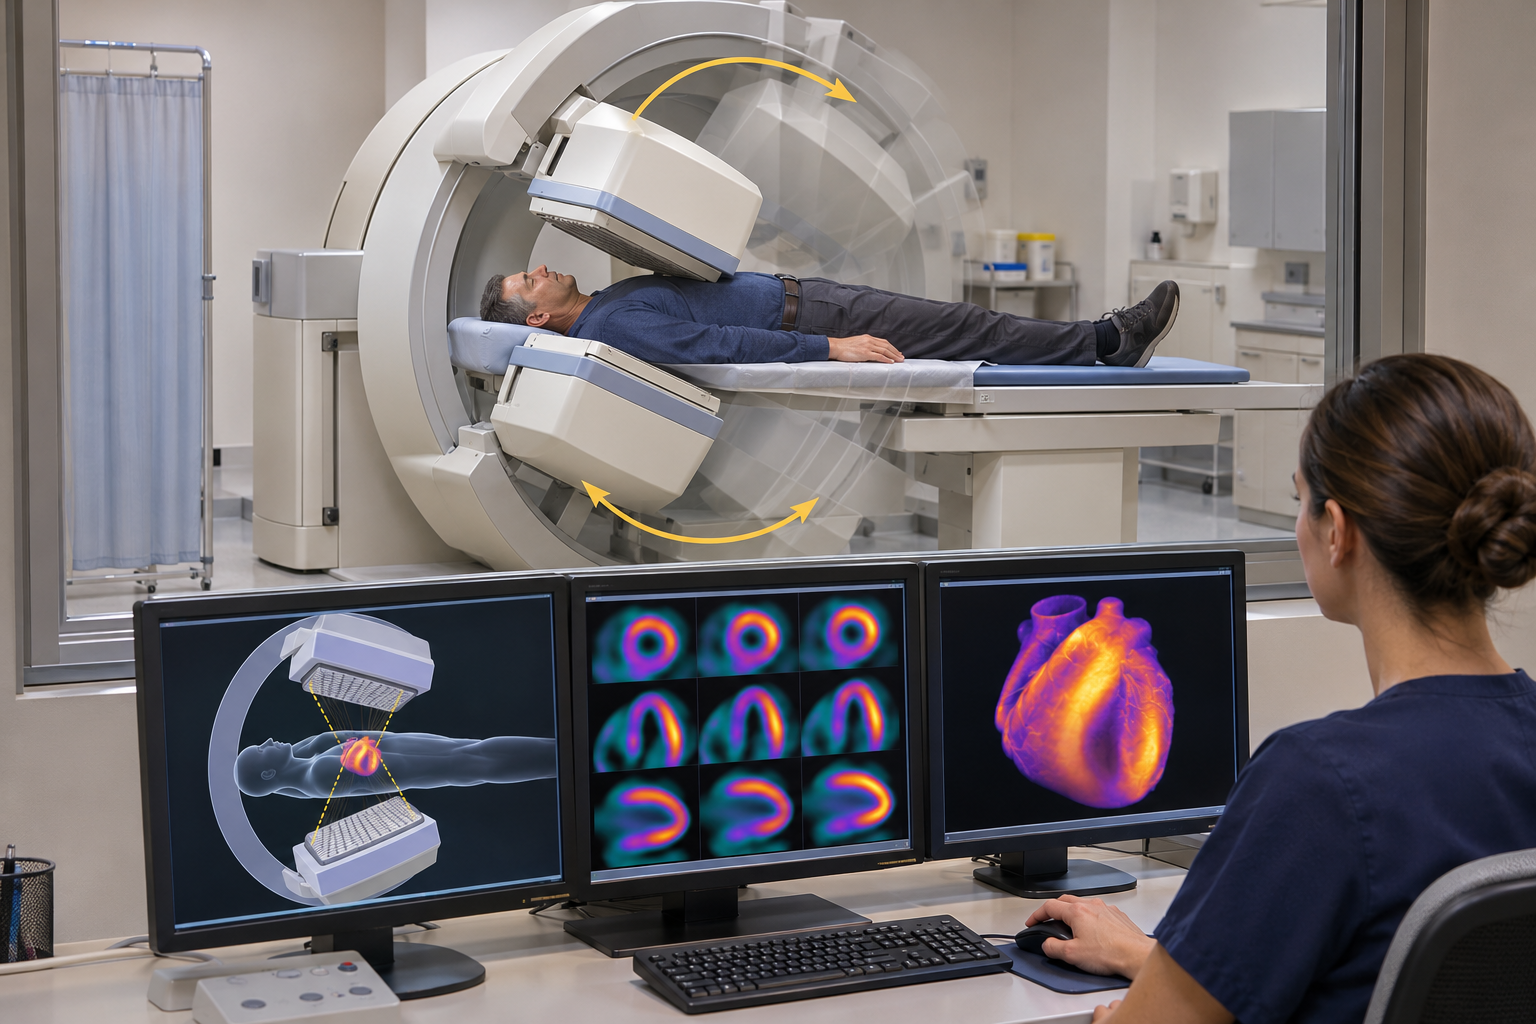
\includegraphics[width=\textwidth,keepaspectratio]{modalities/infographics/spect_realistic.png}
\end{center}
\begin{center}\footnotesize SPECT camera heads rotate around the patient and reconstruct detected single gamma photons into a three-dimensional tracer distribution. AI-generated illustration; perfusion images are not clinical studies.\end{center}

\section{Overview}
Single-Photon Emission Computed Tomography (SPECT) is a nuclear medicine imaging technique that uses gamma cameras to detect photons emitted by radiopharmaceuticals administered to a patient. Computational reconstruction generates three-dimensional images of radiotracer distribution within the body.

Unlike CT and structural MRI, SPECT primarily provides information about physiological function, tissue perfusion, metabolic processes, molecular transport, and receptor availability. It is particularly valuable for myocardial perfusion imaging, skeletal disorders, neurological diseases, parathyroid localization, and infection imaging.

This catalogue focuses specifically on SPECT and SPECT/CT, excluding PET and examinations predominantly performed using planar scintigraphy. 

Some listed examinations are usually performed with planar imaging; they are included only where SPECT or SPECT/CT can provide selected three-dimensional localization, which is identified in the relevant entries.

\section{Where SPECT is used}
The numbered entries summarize characteristic SPECT findings and radiopharmaceuticals. Interpretation should account for the tracer's biological mechanism, acquisition protocol, physiological state, and reconstruction method.

\subsection{Cardiovascular diseases}
\begin{enumerate}[leftmargin=*,itemsep=0.45em,topsep=0.4em]
\item \textbf{Cardiac device infection.} Useful imaging findings include: Abnormal leukocyte uptake around implanted devices. Radiopharmaceutical: ⁹⁹ᵐTc-HMPAO leukocytes.
\item \textbf{Cardiac sympathetic denervation.} Useful imaging findings include: Reduced myocardial sympathetic tracer uptake. Radiopharmaceutical: ¹²³I-MIBG.
\item \textbf{Chronic heart failure.} Useful imaging findings include: Reduced ventricular function and possible perfusion abnormalities. Radiopharmaceutical: ⁹⁹ᵐTc-Sestamibi.
\item \textbf{Coronary artery disease.} Useful imaging findings include: Stress-induced myocardial perfusion defects. Radiopharmaceutical: ⁹⁹ᵐTc-Sestamibi.
\item \textbf{Coronary microvascular dysfunction.} Useful imaging findings include: Reduced myocardial flow reserve on specialized dynamic SPECT. Radiopharmaceutical: ⁹⁹ᵐTc-Sestamibi.
\item \textbf{Dilated cardiomyopathy.} Useful imaging findings include: Ventricular dilatation and reduced ejection fraction. Radiopharmaceutical: ⁹⁹ᵐTc-Sestamibi.
\item \textbf{Hibernating myocardium.} Useful imaging findings include: Preserved or redistributing tracer uptake in dysfunctional myocardium. Radiopharmaceutical: ²⁰¹Tl-Chloride.
\item \textbf{Hypertrophic cardiomyopathy.} Useful imaging findings include: Heterogeneous myocardial perfusion. Radiopharmaceutical: ⁹⁹ᵐTc-Tetrofosmin.
\item \textbf{Ischemic cardiomyopathy.} Useful imaging findings include: Regional perfusion defects and ventricular dysfunction. Radiopharmaceutical: ⁹⁹ᵐTc-Sestamibi.
\item \textbf{Left ventricular aneurysm.} Useful imaging findings include: Fixed perfusion defect and dyskinetic ventricular segment. Radiopharmaceutical: ⁹⁹ᵐTc-Sestamibi.
\item \textbf{Multivessel coronary artery disease.} Useful imaging findings include: Perfusion abnormalities involving multiple vascular territories. Radiopharmaceutical: ⁹⁹ᵐTc-Tetrofosmin.
\item \textbf{Myocardial ischemia.} Useful imaging findings include: Reversible myocardial perfusion defects. Radiopharmaceutical: ⁹⁹ᵐTc-Tetrofosmin.
\item \textbf{Previous myocardial infarction.} Useful imaging findings include: Fixed myocardial perfusion defects. Radiopharmaceutical: ⁹⁹ᵐTc-Sestamibi.
\item \textbf{Prosthetic valve endocarditis.} Useful imaging findings include: Abnormal periprosthetic leukocyte accumulation. Radiopharmaceutical: ⁹⁹ᵐTc-HMPAO leukocytes.
\item \textbf{Transthyretin cardiac amyloidosis.} Useful imaging findings include: Myocardial uptake confirmed on SPECT and interpreted with validated criteria. Radiopharmaceutical: ⁹⁹ᵐTc-PYP, DPD, HMDP.
\end{enumerate}
Myocardial perfusion imaging is one of the most established and widely used clinical applications of SPECT. Balanced ischemia in multivessel coronary disease can, however, produce apparently normal relative perfusion images.
For bone-tracer assessment of ATTR cardiac amyloidosis, evaluate for a monoclonal protein and interpret uptake with the clinical findings; uptake alone does not establish ATTR and can be misleading in AL amyloidosis.

\subsection{Neurological and neurodegenerative diseases}
\begin{enumerate}[leftmargin=*,itemsep=0.45em,topsep=0.4em]
\item \textbf{Alzheimer disease.} Useful imaging findings include: Temporoparietal and posterior cingulate hypoperfusion. Radiopharmaceutical: ⁹⁹ᵐTc-HMPAO.
\item \textbf{Cerebral circulatory arrest.} Useful imaging findings include: Absence of intracranial radiotracer perfusion on a protocol-based ancillary study. Radiopharmaceutical: ⁹⁹ᵐTc-HMPAO.
\item \textbf{Corticobasal syndrome.} Useful imaging findings include: Asymmetric cortical perfusion abnormalities or reduced dopamine transporter binding. Radiopharmaceutical: ⁹⁹ᵐTc-ECD, ¹²³I-Ioflupane.
\item \textbf{Dementia with Lewy bodies.} Useful imaging findings include: Reduced striatal dopamine transporter binding. Radiopharmaceutical: ¹²³I-Ioflupane.
\item \textbf{Drug-induced parkinsonism.} Useful imaging findings include: Usually preserved dopamine transporter binding in pure drug-induced cases. Radiopharmaceutical: ¹²³I-Ioflupane.
\item \textbf{Essential tremor.} Useful imaging findings include: Usually preserved striatal dopamine transporter binding. Radiopharmaceutical: ¹²³I-Ioflupane.
\item \textbf{Frontotemporal dementia.} Useful imaging findings include: Frontal and anterior temporal hypoperfusion. Radiopharmaceutical: ⁹⁹ᵐTc-ECD.
\item \textbf{Huntington disease.} Useful imaging findings include: Reported basal ganglia perfusion abnormalities. Radiopharmaceutical: ⁹⁹ᵐTc-HMPAO.
\item \textbf{Hypoxic-ischemic brain injury.} Useful imaging findings include: Regional or widespread perfusion reduction. Radiopharmaceutical: ⁹⁹ᵐTc-ECD.
\item \textbf{Multiple system atrophy.} Useful imaging findings include: Reduced striatal dopamine transporter binding. Radiopharmaceutical: ¹²³I-Ioflupane.
\item \textbf{Normal pressure hydrocephalus.} Useful imaging findings include: Variable cerebral perfusion abnormalities. Radiopharmaceutical: ⁹⁹ᵐTc-ECD.
\item \textbf{Parkinson disease.} Useful imaging findings include: Reduced striatal dopamine transporter binding. Radiopharmaceutical: ¹²³I-Ioflupane.
\item \textbf{Progressive supranuclear palsy.} Useful imaging findings include: Reduced striatal dopamine transporter binding. Radiopharmaceutical: ¹²³I-Ioflupane.
\item \textbf{Vascular dementia.} Useful imaging findings include: Multifocal cerebral perfusion abnormalities. Radiopharmaceutical: ⁹⁹ᵐTc-HMPAO.
\end{enumerate}
Dopamine transporter SPECT (DaT-SPECT) can help distinguish degenerative parkinsonian syndromes from certain nondegenerative causes of tremor. It cannot reliably distinguish Parkinson disease from multiple system atrophy or progressive supranuclear palsy.
Radionuclide cerebral perfusion imaging may serve as an ancillary test in death by neurologic criteria when performed and interpreted under applicable protocols; the scan alone does not establish that clinical diagnosis.

\subsection{Epilepsy}
\begin{enumerate}[leftmargin=*,itemsep=0.45em,topsep=0.4em]
\item \textbf{Drug-resistant focal epilepsy.} Useful imaging findings include: Regional ictal hyperperfusion associated with seizure onset or propagation. Radiopharmaceutical: ⁹⁹ᵐTc-HMPAO.
\item \textbf{Focal cortical dysplasia.} Useful imaging findings include: Abnormal ictal regional perfusion. Radiopharmaceutical: ⁹⁹ᵐTc-HMPAO.
\item \textbf{Frontal lobe epilepsy.} Useful imaging findings include: Ictal frontal hyperperfusion. Radiopharmaceutical: ⁹⁹ᵐTc-ECD.
\item \textbf{Mesial temporal sclerosis.} Useful imaging findings include: Variable interictal temporal hypoperfusion. Radiopharmaceutical: ⁹⁹ᵐTc-ECD.
\item \textbf{MRI-negative focal epilepsy.} Useful imaging findings include: Potential localization of seizure-related perfusion abnormalities. Radiopharmaceutical: ⁹⁹ᵐTc-HMPAO.
\item \textbf{Occipital lobe epilepsy.} Useful imaging findings include: Ictal occipital hyperperfusion. Radiopharmaceutical: ⁹⁹ᵐTc-HMPAO.
\item \textbf{Parietal lobe epilepsy.} Useful imaging findings include: Ictal parietal hyperperfusion. Radiopharmaceutical: ⁹⁹ᵐTc-ECD.
\item \textbf{Temporal lobe epilepsy.} Useful imaging findings include: Ictal temporal hyperperfusion. Radiopharmaceutical: ⁹⁹ᵐTc-HMPAO.
\end{enumerate}
A specialized computational technique called SISCOM (Subtraction Ictal SPECT Co-registered to MRI) compares ictal and interictal SPECT studies to help localize epileptogenic regions before surgery.

\subsection{Cerebrovascular diseases}
\begin{enumerate}[leftmargin=*,itemsep=0.45em,topsep=0.4em]
\item \textbf{Carotid artery occlusion.} Useful imaging findings include: Regional hypoperfusion. Radiopharmaceutical: ⁹⁹ᵐTc-ECD.
\item \textbf{Carotid artery stenosis.} Useful imaging findings include: Reduced cerebrovascular perfusion reserve. Radiopharmaceutical: ⁹⁹ᵐTc-HMPAO.
\item \textbf{Cerebral hyperperfusion syndrome.} Useful imaging findings include: Increased regional perfusion following revascularization. Radiopharmaceutical: ⁹⁹ᵐTc-ECD.
\item \textbf{Cerebral small vessel disease.} Useful imaging findings include: Heterogeneous cerebral perfusion. Radiopharmaceutical: ⁹⁹ᵐTc-HMPAO.
\item \textbf{Cerebral vasospasm.} Useful imaging findings include: Regional perfusion reduction. Radiopharmaceutical: ⁹⁹ᵐTc-ECD.
\item \textbf{Chronic cerebral ischemia.} Useful imaging findings include: Persistently reduced regional perfusion. Radiopharmaceutical: ⁹⁹ᵐTc-ECD.
\item \textbf{Ischemic stroke.} Useful imaging findings include: Regional cerebral hypoperfusion. Radiopharmaceutical: ⁹⁹ᵐTc-HMPAO.
\item \textbf{Moyamoya disease.} Useful imaging findings include: Impaired cerebral perfusion and vascular reserve. Radiopharmaceutical: ⁹⁹ᵐTc-HMPAO.
\end{enumerate}
Most acute cerebrovascular diseases are now investigated primarily using CT, CT angiography, or MRI. SPECT remains useful in selected cerebral perfusion and vascular reserve assessments.

\subsection{Pulmonary diseases}
\begin{enumerate}[leftmargin=*,itemsep=0.45em,topsep=0.4em]
\item \textbf{Acute pulmonary embolism.} Useful imaging findings include: Segmental ventilation-perfusion mismatch. Radiopharmaceutical: ⁹⁹ᵐTc-MAA and Technegas.
\item \textbf{Chronic obstructive pulmonary disease.} Useful imaging findings include: Heterogeneous ventilation and perfusion. Radiopharmaceutical: ⁹⁹ᵐTc-MAA and Technegas.
\item \textbf{Chronic pulmonary embolism.} Useful imaging findings include: Persistent regional perfusion defects; ventilation imaging helps determine whether defects are mismatched. Radiopharmaceutical: ⁹⁹ᵐTc-MAA; add a ventilation agent when performing V/Q imaging.
\item \textbf{Chronic thromboembolic pulmonary hypertension.} Useful imaging findings include: Persistent mismatched ventilation-perfusion defects. Radiopharmaceutical: ⁹⁹ᵐTc-MAA and a ventilation agent (e.g., ⁹⁹ᵐTc-Technegas or aerosol).
\item \textbf{Pneumonia.} Useful imaging findings include: Ventilation and perfusion abnormalities, sometimes with reverse mismatch. Radiopharmaceutical: ⁹⁹ᵐTc-MAA and Technegas.
\item \textbf{Pulmonary artery obstruction.} Useful imaging findings include: Regional absence of pulmonary perfusion. Radiopharmaceutical: ⁹⁹ᵐTc-MAA.
\item \textbf{Pulmonary artery stenosis.} Useful imaging findings include: Reduced perfusion within the affected lung region. Radiopharmaceutical: ⁹⁹ᵐTc-MAA.
\item \textbf{Pulmonary emphysema.} Useful imaging findings include: Regional reductions in ventilation and perfusion. Radiopharmaceutical: ⁹⁹ᵐTc-MAA and Technegas.
\item \textbf{Pulmonary fibrosis (selected preoperative regional function assessment).} Useful imaging findings include: Regional perfusion contribution to lung function; does not diagnose pulmonary fibrosis. Radiopharmaceutical: ⁹⁹ᵐTc-MAA.
\end{enumerate}

\subsection{Thyroid and parathyroid diseases}
\begin{enumerate}[leftmargin=*,itemsep=0.45em,topsep=0.4em]
\item \textbf{Ectopic parathyroid adenoma.} Useful imaging findings include: Focal uptake outside the expected parathyroid location. Radiopharmaceutical: ⁹⁹ᵐTc-Sestamibi.
\item \textbf{Ectopic thyroid tissue.} Useful imaging findings include: Uptake at an abnormal anatomical location; SPECT/CT may aid localization. Radiopharmaceutical: ⁹⁹ᵐTc-Pertechnetate.
\item \textbf{Follicular thyroid carcinoma.} Useful imaging findings include: Radioiodine-avid metastases; SPECT/CT is a localization adjunct. Radiopharmaceutical: ¹³¹I.
\item \textbf{Papillary thyroid carcinoma.} Useful imaging findings include: Radioiodine-avid residual or metastatic tissue; SPECT/CT adds localization to planar imaging. Radiopharmaceutical: ¹³¹I.
\item \textbf{Parathyroid adenoma.} Useful imaging findings include: Persistent focal radiotracer retention. Radiopharmaceutical: ⁹⁹ᵐTc-Sestamibi.
\item \textbf{Parathyroid carcinoma.} Useful imaging findings include: Possible increased focal tracer uptake. Radiopharmaceutical: ⁹⁹ᵐTc-Sestamibi.
\item \textbf{Parathyroid hyperplasia.} Useful imaging findings include: Abnormal uptake involving one or more glands. Radiopharmaceutical: ⁹⁹ᵐTc-Sestamibi.
\item \textbf{Recurrent hyperparathyroidism.} Useful imaging findings include: Focal uptake corresponding to residual or recurrent hyperfunctioning tissue. Radiopharmaceutical: ⁹⁹ᵐTc-Sestamibi.
\item \textbf{Retrosternal goiter.} Useful imaging findings include: Thyroid tracer uptake extending into the mediastinum. Radiopharmaceutical: ¹²³I.
\item \textbf{Thyroid cancer bone metastases.} Useful imaging findings include: Focal skeletal radioiodine uptake; SPECT/CT may localize selected lesions. Radiopharmaceutical: ¹³¹I.
\item \textbf{Thyroid cancer lymph node metastases.} Useful imaging findings include: Focal radioiodine uptake; SPECT/CT may anatomically localize selected lesions. Radiopharmaceutical: ¹³¹I.
\item \textbf{Thyroid cancer pulmonary metastases.} Useful imaging findings include: Focal or diffuse pulmonary radioiodine uptake, generally assessed on planar imaging. Radiopharmaceutical: ¹³¹I.
\end{enumerate}
Routine thyroid function scintigraphy is generally performed using planar imaging. SPECT/CT is particularly helpful when precise anatomical localization is required.
Radioiodine whole-body imaging for thyroid cancer is commonly acquired as planar imaging; SPECT/CT is an adjunct for anatomical localization or characterization of selected findings.

\subsection{Bone and skeletal diseases}
\begin{enumerate}[leftmargin=*,itemsep=0.45em,topsep=0.4em]
\item \textbf{Acute osteomyelitis.} Useful imaging findings include: Increased uptake in infected skeletal structures. Radiopharmaceutical: ⁹⁹ᵐTc-MDP.
\item \textbf{Breast cancer bone metastases.} Useful imaging findings include: Focal or multifocal increased skeletal uptake. Radiopharmaceutical: ⁹⁹ᵐTc-MDP.
\item \textbf{Chronic osteomyelitis.} Useful imaging findings include: Abnormal osseous uptake or leukocyte accumulation. Radiopharmaceutical: Labeled leukocytes.
\item \textbf{Delayed fracture union.} Useful imaging findings include: Variable abnormal uptake at fracture site. Radiopharmaceutical: ⁹⁹ᵐTc-MDP.
\item \textbf{Ewing sarcoma.} Useful imaging findings include: Variable increased skeletal uptake. Radiopharmaceutical: ⁹⁹ᵐTc-MDP.
\item \textbf{Femoral neck stress fracture.} Useful imaging findings include: Focal increased femoral neck uptake. Radiopharmaceutical: ⁹⁹ᵐTc-MDP.
\item \textbf{Fibrous dysplasia.} Useful imaging findings include: Increased skeletal remodeling activity. Radiopharmaceutical: ⁹⁹ᵐTc-MDP.
\item \textbf{Fracture nonunion.} Useful imaging findings include: Abnormal uptake reflecting residual biological activity. Radiopharmaceutical: ⁹⁹ᵐTc-MDP.
\item \textbf{Heterotopic ossification.} Useful imaging findings include: Increased extraosseous tracer accumulation. Radiopharmaceutical: ⁹⁹ᵐTc-MDP.
\item \textbf{Hypertrophic osteoarthropathy.} Useful imaging findings include: Symmetrical periosteal uptake. Radiopharmaceutical: ⁹⁹ᵐTc-MDP.
\item \textbf{Insufficiency fracture.} Useful imaging findings include: Increased uptake within mechanically weakened bone. Radiopharmaceutical: ⁹⁹ᵐTc-MDP.
\item \textbf{Medial tibial stress syndrome.} Useful imaging findings include: Longitudinal increased tibial uptake. Radiopharmaceutical: ⁹⁹ᵐTc-MDP.
\item \textbf{Occult fracture.} Useful imaging findings include: Focal skeletal tracer accumulation. Radiopharmaceutical: ⁹⁹ᵐTc-MDP.
\item \textbf{Osteoblastic bone metastases.} Useful imaging findings include: Multifocal increased skeletal uptake. Radiopharmaceutical: ⁹⁹ᵐTc-MDP.
\item \textbf{Osteoblastoma.} Useful imaging findings include: Increased uptake within affected bone. Radiopharmaceutical: ⁹⁹ᵐTc-MDP.
\item \textbf{Osteochondral lesion of the talus.} Useful imaging findings include: Focal subchondral tracer accumulation. Radiopharmaceutical: ⁹⁹ᵐTc-MDP.
\item \textbf{Osteoid osteoma.} Useful imaging findings include: Intense focal tracer uptake. Radiopharmaceutical: ⁹⁹ᵐTc-MDP.
\item \textbf{Osteonecrosis.} Useful imaging findings include: Reduced uptake in necrotic regions or increased reparative uptake. Radiopharmaceutical: ⁹⁹ᵐTc-MDP.
\item \textbf{Osteosarcoma.} Useful imaging findings include: Increased uptake in mineralizing tumor components. Radiopharmaceutical: ⁹⁹ᵐTc-MDP.
\item \textbf{Paget disease of bone.} Useful imaging findings include: Intense uptake involving affected bone. Radiopharmaceutical: ⁹⁹ᵐTc-MDP.
\item \textbf{Prostate cancer bone metastases.} Useful imaging findings include: Increased osteoblastic activity. Radiopharmaceutical: ⁹⁹ᵐTc-MDP.
\item \textbf{Sacral insufficiency fracture.} Useful imaging findings include: Characteristic sacral uptake, sometimes H-shaped. Radiopharmaceutical: ⁹⁹ᵐTc-MDP.
\item \textbf{Stress fracture.} Useful imaging findings include: Focal or linear increased bone uptake. Radiopharmaceutical: ⁹⁹ᵐTc-MDP.
\item \textbf{Vertebral compression fracture.} Useful imaging findings include: Increased uptake in active or healing fractures. Radiopharmaceutical: ⁹⁹ᵐTc-MDP.
\end{enumerate}

\subsection{Joint and prosthetic disorders}
\begin{enumerate}[leftmargin=*,itemsep=0.45em,topsep=0.4em]
\item \textbf{Aseptic prosthetic loosening.} Useful imaging findings include: Increased uptake at prosthetic interfaces. Radiopharmaceutical: ⁹⁹ᵐTc-MDP.
\item \textbf{Charcot arthropathy.} Useful imaging findings include: Increased joint and skeletal remodeling activity. Radiopharmaceutical: ⁹⁹ᵐTc-MDP.
\item \textbf{Complex regional pain syndrome.} Useful imaging findings include: Variable periarticular uptake abnormalities. Radiopharmaceutical: ⁹⁹ᵐTc-MDP.
\item \textbf{Mandibular condylar hyperplasia.} Useful imaging findings include: Asymmetric increased condylar uptake. Radiopharmaceutical: ⁹⁹ᵐTc-MDP.
\item \textbf{Osteoarthritis.} Useful imaging findings include: Increased subchondral bone turnover. Radiopharmaceutical: ⁹⁹ᵐTc-MDP.
\item \textbf{Painful total hip arthroplasty.} Useful imaging findings include: Abnormal acetabular or femoral component uptake. Radiopharmaceutical: ⁹⁹ᵐTc-MDP.
\item \textbf{Painful total knee arthroplasty.} Useful imaging findings include: Abnormal compartmental or periprosthetic uptake. Radiopharmaceutical: ⁹⁹ᵐTc-MDP.
\item \textbf{Patellofemoral osteoarthritis.} Useful imaging findings include: Increased patellofemoral tracer uptake. Radiopharmaceutical: ⁹⁹ᵐTc-MDP.
\item \textbf{Prosthetic joint infection.} Useful imaging findings include: Abnormal periprosthetic leukocyte accumulation; interpretation may require complementary bone or marrow imaging. Radiopharmaceutical: ¹¹¹In-oxine leukocytes, with bone or marrow imaging as indicated.
\item \textbf{Rheumatoid arthritis.} Useful imaging findings include: Increased periarticular skeletal uptake. Radiopharmaceutical: ⁹⁹ᵐTc-MDP.
\item \textbf{Sacroiliac joint dysfunction.} Useful imaging findings include: Variable increased sacroiliac uptake. Radiopharmaceutical: ⁹⁹ᵐTc-MDP.
\item \textbf{Sacroiliitis.} Useful imaging findings include: Increased sacroiliac bone turnover in some cases. Radiopharmaceutical: ⁹⁹ᵐTc-MDP.
\item \textbf{Septic arthritis.} Useful imaging findings include: Increased inflammatory tracer accumulation. Radiopharmaceutical: Labeled leukocytes.
\item \textbf{Temporomandibular joint degeneration.} Useful imaging findings include: Increased condylar uptake. Radiopharmaceutical: ⁹⁹ᵐTc-MDP.
\end{enumerate}

\subsection{Spine disorders}
\begin{enumerate}[leftmargin=*,itemsep=0.45em,topsep=0.4em]
\item \textbf{Baastrup disease.} Useful imaging findings include: Increased uptake between adjacent spinous processes. Radiopharmaceutical: ⁹⁹ᵐTc-MDP.
\item \textbf{Cervical facet arthropathy.} Useful imaging findings include: Focal increased facet joint uptake. Radiopharmaceutical: ⁹⁹ᵐTc-MDP.
\item \textbf{Degenerative disc disease.} Useful imaging findings include: Increased uptake at adjacent vertebral endplates. Radiopharmaceutical: ⁹⁹ᵐTc-MDP.
\item \textbf{Lumbar facet arthropathy.} Useful imaging findings include: Increased facet joint uptake. Radiopharmaceutical: ⁹⁹ᵐTc-MDP.
\item \textbf{Spinal fusion pseudarthrosis.} Useful imaging findings include: Persistent focal uptake at fusion site. Radiopharmaceutical: ⁹⁹ᵐTc-MDP.
\item \textbf{Spinal hardware loosening.} Useful imaging findings include: Increased uptake around orthopedic instrumentation. Radiopharmaceutical: ⁹⁹ᵐTc-MDP.
\item \textbf{Spinal metastases.} Useful imaging findings include: Focal abnormal vertebral uptake. Radiopharmaceutical: ⁹⁹ᵐTc-MDP.
\item \textbf{Spondylodiscitis.} Useful imaging findings include: Increased uptake involving adjacent vertebral endplates. Radiopharmaceutical: ⁶⁷Ga-Citrate, ⁹⁹ᵐTc-MDP.
\item \textbf{Spondylolisthesis.} Useful imaging findings include: Abnormal uptake in mechanically stressed structures. Radiopharmaceutical: ⁹⁹ᵐTc-MDP.
\item \textbf{Spondylolysis.} Useful imaging findings include: Increased uptake within an active pars interarticularis lesion. Radiopharmaceutical: ⁹⁹ᵐTc-MDP.
\item \textbf{Vertebral osteomyelitis.} Useful imaging findings include: Abnormal vertebral skeletal or inflammatory uptake. Radiopharmaceutical: ⁹⁹ᵐTc-MDP.
\end{enumerate}

\subsection{Infectious and inflammatory diseases}
\begin{enumerate}[leftmargin=*,itemsep=0.45em,topsep=0.4em]
\item \textbf{Crohn disease.} Useful imaging findings include: Segmental inflammatory bowel uptake. Radiopharmaceutical: ⁹⁹ᵐTc-HMPAO leukocytes.
\item \textbf{Diabetic foot osteomyelitis.} Useful imaging findings include: Abnormal leukocyte accumulation within bone. Radiopharmaceutical: ⁹⁹ᵐTc-HMPAO leukocytes.
\item \textbf{Diabetic foot soft-tissue infection.} Useful imaging findings include: Leukocyte uptake confined to soft tissues. Radiopharmaceutical: ⁹⁹ᵐTc-HMPAO leukocytes.
\item \textbf{Fever of unknown origin.} Useful imaging findings include: Potential localization of occult inflammatory or infectious foci. Radiopharmaceutical: ⁶⁷Ga-Citrate.
\item \textbf{Infected orthopedic hardware.} Useful imaging findings include: Abnormal peri-implant leukocyte accumulation; correlate with bone or marrow imaging when indicated. Radiopharmaceutical: ¹¹¹In-oxine leukocytes, with bone or marrow imaging as indicated.
\item \textbf{Inflammatory bowel disease.} Useful imaging findings include: Increased bowel leukocyte accumulation. Radiopharmaceutical: ⁹⁹ᵐTc-HMPAO leukocytes.
\item \textbf{Intra-abdominal abscess.} Useful imaging findings include: Focal leukocyte accumulation. Radiopharmaceutical: ¹¹¹In-Oxine leukocytes.
\item \textbf{Occult infection.} Useful imaging findings include: Abnormal localized inflammatory tracer uptake. Radiopharmaceutical: Labeled leukocytes.
\item \textbf{Pulmonary tuberculosis.} Useful imaging findings include: Abnormal inflammatory tracer accumulation. Radiopharmaceutical: ⁶⁷Ga-Citrate.
\item \textbf{Sarcoidosis.} Useful imaging findings include: Increased inflammatory tracer uptake. Radiopharmaceutical: ⁶⁷Ga-Citrate.
\item \textbf{Ulcerative colitis.} Useful imaging findings include: Increased colonic leukocyte accumulation. Radiopharmaceutical: ⁹⁹ᵐTc-HMPAO leukocytes.
\item \textbf{Vascular graft infection.} Useful imaging findings include: Abnormal leukocyte uptake surrounding vascular graft. Radiopharmaceutical: ⁹⁹ᵐTc-HMPAO leukocytes.
\end{enumerate}
Several gallium-67 and labeled leukocyte examinations have been superseded by FDG-PET/CT or other modalities in many clinical settings.

\subsection{Neuroendocrine and adrenal tumors}
\begin{enumerate}[leftmargin=*,itemsep=0.45em,topsep=0.4em]
\item \textbf{Aldosterone-producing adrenal adenoma.} Useful imaging findings include: Asymmetric adrenal cortical tracer uptake. Radiopharmaceutical: ¹³¹I-NP-59.
\item \textbf{Autonomous adrenal cortisol production.} Useful imaging findings include: Asymmetric adrenal cortical tracer uptake. Radiopharmaceutical: ¹³¹I-NP-59.
\item \textbf{Bronchial carcinoid.} Useful imaging findings include: Increased somatostatin receptor uptake. Radiopharmaceutical: ¹¹¹In-Pentetreotide.
\item \textbf{Gastrinoma.} Useful imaging findings include: Abnormal receptor-specific uptake. Radiopharmaceutical: ¹¹¹In-Pentetreotide.
\item \textbf{Gastroenteropancreatic neuroendocrine tumor.} Useful imaging findings include: Increased somatostatin receptor tracer uptake. Radiopharmaceutical: ¹¹¹In-Pentetreotide.
\item \textbf{Metastatic neuroblastoma.} Useful imaging findings include: Multifocal MIBG-avid lesions. Radiopharmaceutical: ¹²³I-MIBG.
\item \textbf{Metastatic pheochromocytoma.} Useful imaging findings include: Abnormal MIBG uptake in metastatic lesions. Radiopharmaceutical: ¹²³I-MIBG.
\item \textbf{Neuroblastoma.} Useful imaging findings include: Increased catecholamine transporter-related uptake. Radiopharmaceutical: ¹²³I-MIBG.
\item \textbf{Pancreatic neuroendocrine tumor.} Useful imaging findings include: Focal receptor-specific tracer accumulation. Radiopharmaceutical: ¹¹¹In-Pentetreotide.
\item \textbf{Paraganglioma.} Useful imaging findings include: Focal extra-adrenal MIBG accumulation. Radiopharmaceutical: ¹²³I-MIBG.
\item \textbf{Pheochromocytoma.} Useful imaging findings include: Abnormal adrenal MIBG accumulation. Radiopharmaceutical: ¹²³I-MIBG.
\item \textbf{Small bowel neuroendocrine tumor.} Useful imaging findings include: Increased receptor-specific uptake. Radiopharmaceutical: ¹¹¹In-Pentetreotide.
\end{enumerate}
Somatostatin receptor PET/CT has largely replaced conventional indium-111 receptor scintigraphy where available. Adrenal cortical scintigraphy with NP-59 is now uncommon.

\subsection{Renal and urinary diseases}
\begin{enumerate}[leftmargin=*,itemsep=0.45em,topsep=0.4em]
\item \textbf{Acute pyelonephritis.} Useful imaging findings include: Focal renal cortical uptake defects. Radiopharmaceutical: ⁹⁹ᵐTc-DMSA.
\item \textbf{Duplex kidney.} Useful imaging findings include: Abnormal renal cortical configuration. Radiopharmaceutical: ⁹⁹ᵐTc-DMSA.
\item \textbf{Ectopic kidney.} Useful imaging findings include: Functioning renal tissue at an abnormal anatomical location. Radiopharmaceutical: ⁹⁹ᵐTc-DMSA.
\item \textbf{Horseshoe kidney.} Useful imaging findings include: Abnormal three-dimensional renal configuration. Radiopharmaceutical: ⁹⁹ᵐTc-DMSA.
\item \textbf{Reflux nephropathy.} Useful imaging findings include: Abnormal cortical tracer distribution. Radiopharmaceutical: ⁹⁹ᵐTc-DMSA.
\item \textbf{Renal cortical scarring.} Useful imaging findings include: Persistent cortical tracer defects. Radiopharmaceutical: ⁹⁹ᵐTc-DMSA.
\item \textbf{Renal dysplasia.} Useful imaging findings include: Reduced or heterogeneous cortical uptake. Radiopharmaceutical: ⁹⁹ᵐTc-DMSA.
\item \textbf{Renal infarction.} Useful imaging findings include: Regional absence of cortical uptake. Radiopharmaceutical: ⁹⁹ᵐTc-DMSA.
\end{enumerate}
SPECT provides supplementary three-dimensional renal cortical information. Dynamic renal functional studies are predominantly performed using conventional gamma-camera renography.

\subsection{Hepatobiliary, gastrointestinal and splenic diseases}
\begin{enumerate}[leftmargin=*,itemsep=0.45em,topsep=0.4em]
\item \textbf{Accessory spleen (selected SPECT/CT localization).} Useful imaging findings include: Focal uptake corresponding to functioning splenic tissue; planar imaging is also used. Radiopharmaceutical: ⁹⁹ᵐTc-Heat-damaged RBCs.
\item \textbf{Active gastrointestinal bleeding (selected SPECT localization).} Useful imaging findings include: Extravascular blood-pool accumulation; planar imaging is generally performed first. Radiopharmaceutical: ⁹⁹ᵐTc-labeled RBCs.
\item \textbf{Bile leak (selected SPECT/CT localization).} Useful imaging findings include: Extraluminal biliary tracer; planar hepatobiliary imaging is generally the initial study. Radiopharmaceutical: ⁹⁹ᵐTc-Mebrofenin.
\item \textbf{Focal nodular hyperplasia (selected SPECT/CT characterization).} Useful imaging findings include: Preserved or increased colloid uptake in some lesions; planar imaging is commonly used. Radiopharmaceutical: ⁹⁹ᵐTc-Sulfur colloid.
\item \textbf{Functional splenic tissue within an abdominal mass (selected SPECT/CT localization).} Useful imaging findings include: Selective splenic tracer accumulation; planar imaging is also used. Radiopharmaceutical: ⁹⁹ᵐTc-Heat-damaged RBCs.
\item \textbf{Hepatic hemangioma (selected SPECT/CT localization).} Useful imaging findings include: Delayed blood-pool tracer accumulation; planar blood-pool imaging is commonly used first. Radiopharmaceutical: ⁹⁹ᵐTc-labeled RBCs.
\item \textbf{Intrahepatic hepatopulmonary shunting before radioembolization.} Useful imaging findings include: Planar imaging quantifies pulmonary shunting; SPECT/CT may provide selected localization. Radiopharmaceutical: ⁹⁹ᵐTc-MAA.
\item \textbf{Meckel diverticulum (selected SPECT/CT localization).} Useful imaging findings include: Ectopic gastric mucosal tracer uptake; SPECT/CT may clarify equivocal planar findings. Radiopharmaceutical: ⁹⁹ᵐTc-Pertechnetate.
\item \textbf{Splenosis (selected SPECT/CT localization).} Useful imaging findings include: Tracer uptake within ectopic splenic tissue; planar imaging is also used. Radiopharmaceutical: ⁹⁹ᵐTc-Heat-damaged RBCs.
\end{enumerate}

\subsection{Lymphatic disorders and oncological localization}
\begin{enumerate}[leftmargin=*,itemsep=0.45em,topsep=0.4em]
\item \textbf{Breast carcinoma sentinel node localization.} Useful imaging findings include: Identification of draining sentinel lymph nodes. Radiopharmaceutical: ⁹⁹ᵐTc-Nanocolloid.
\item \textbf{Chylous leakage.} Useful imaging findings include: Abnormal lymphatic tracer accumulation. Radiopharmaceutical: ⁹⁹ᵐTc-Nanocolloid.
\item \textbf{Lymphatic obstruction.} Useful imaging findings include: Interrupted or delayed lymphatic drainage. Radiopharmaceutical: ⁹⁹ᵐTc-Nanocolloid.
\item \textbf{Malignant melanoma sentinel node localization.} Useful imaging findings include: Identification of regional draining lymph nodes. Radiopharmaceutical: ⁹⁹ᵐTc-Nanocolloid.
\item \textbf{Oral carcinoma sentinel node localization.} Useful imaging findings include: Localization of cervical sentinel nodes. Radiopharmaceutical: ⁹⁹ᵐTc-Nanocolloid.
\item \textbf{Penile carcinoma sentinel node localization.} Useful imaging findings include: Localization of inguinal sentinel nodes. Radiopharmaceutical: ⁹⁹ᵐTc-Nanocolloid.
\item \textbf{Primary lymphedema.} Useful imaging findings include: Abnormal lymphatic drainage and dermal backflow. Radiopharmaceutical: ⁹⁹ᵐTc-Nanocolloid.
\item \textbf{Secondary lymphedema.} Useful imaging findings include: Impaired lymphatic transport. Radiopharmaceutical: ⁹⁹ᵐTc-Nanocolloid.
\end{enumerate}
Lymphoscintigraphy and sentinel-node mapping commonly use planar imaging; SPECT/CT is a selected adjunct when planar localization is inadequate or anatomically complex. Sentinel-node imaging identifies drainage pathways and does not establish whether nodes contain malignant cells.

\subsection{Breast diseases}
Dedicated molecular breast imaging generally uses planar gamma-camera systems. The entries below refer only to specialized or limited dedicated breast SPECT applications and are not routine indications for conventional SPECT.
\begin{enumerate}[leftmargin=*,itemsep=0.45em,topsep=0.4em]
\item \textbf{Invasive ductal carcinoma.} Useful imaging findings include: Focal increased radiotracer accumulation. Radiopharmaceutical: ⁹⁹ᵐTc-Sestamibi.
\item \textbf{Invasive lobular carcinoma.} Useful imaging findings include: Variable increased tracer uptake. Radiopharmaceutical: ⁹⁹ᵐTc-Sestamibi.
\item \textbf{Multifocal breast carcinoma.} Useful imaging findings include: Multiple regions of abnormal tracer accumulation. Radiopharmaceutical: ⁹⁹ᵐTc-Sestamibi.
\item \textbf{Recurrent breast carcinoma.} Useful imaging findings include: Abnormal focal tracer uptake. Radiopharmaceutical: ⁹⁹ᵐTc-Sestamibi.
\end{enumerate}
These are specialized or limited applications rather than standard indications for conventional SPECT.

\subsection{Summary of catalogue}
\begin{center}
\begin{tabular}{@{}p{0.70\textwidth}r@{}}
\toprule
\textbf{Disease category} & \textbf{Entries} \\
\midrule
Bone and skeletal diseases & 24 \\
Breast diseases & 4 \\
Cardiovascular diseases & 15 \\
Cerebrovascular diseases & 8 \\
Epilepsy & 8 \\
Hepatobiliary, gastrointestinal and splenic diseases & 9 \\
Infectious and inflammatory diseases & 12 \\
Joint and prosthetic disorders & 14 \\
Lymphatic disorders and oncological localization & 8 \\
Neuroendocrine and adrenal tumors & 12 \\
Neurological and neurodegenerative diseases & 14 \\
Pulmonary diseases & 9 \\
Renal and urinary diseases & 8 \\
Spine disorders & 11 \\
Thyroid and parathyroid diseases & 12 \\
\midrule
\textbf{Total} & \textbf{168} \\
\bottomrule
\end{tabular}
\end{center}

\subsection{Types of SPECT imaging}
\begin{longtable}{@{}p{0.38\textwidth}p{0.54\textwidth}@{}}
\toprule
\textbf{Technique} & \textbf{Primary application} \\
\midrule
\endfirsthead
\toprule
\textbf{Technique} & \textbf{Primary application} \\
\midrule
\endhead
Bone SPECT/CT & Skeletal remodeling and lesion localization \\
Cerebral perfusion SPECT & Regional cerebral blood flow assessment \\
Conventional SPECT & Three-dimensional radiotracer distribution \\
CZT-SPECT & High-sensitivity semiconductor detector imaging \\
Dopamine transporter SPECT & Degenerative parkinsonian syndromes \\
Dynamic SPECT & Time-dependent radiotracer distribution \\
Gated SPECT & Cardiac motion and ventricular function \\
Ictal SPECT & Seizure localization \\
Interictal SPECT & Baseline cerebral perfusion \\
Leukocyte SPECT/CT & Infection localization \\
Pinhole SPECT & High-resolution imaging of small structures \\
Quantitative SPECT & Absolute or relative radiotracer concentration \\
Somatostatin receptor SPECT & Neuroendocrine tumor imaging \\
SPECT/CT & Combined functional and anatomical imaging \\
Stress-rest myocardial SPECT & Myocardial ischemia and infarction \\
Ventilation-perfusion SPECT & Pulmonary embolism \\
\bottomrule
\end{longtable}

\subsection{Major SPECT radiopharmaceuticals}
\begin{longtable}{@{}p{0.30\textwidth}p{0.40\textwidth}p{0.22\textwidth}@{}}
\toprule
\textbf{Radiopharmaceutical} & \textbf{Biological process or target} & \textbf{Photon energy} \\
\midrule
\endfirsthead
\toprule
\textbf{Radiopharmaceutical} & \textbf{Biological process or target} & \textbf{Photon energy} \\
\midrule
\endhead
²⁰¹Tl-Chloride & Perfusion and myocardial viability & Approximately 68--80 keV, additional emissions \\
¹²³I-Ioflupane & Dopamine transporters & 159 keV \\
¹²³I-MIBG & Norepinephrine transport & 159 keV \\
¹³¹I-Sodium iodide & Thyroid iodine transport & 364 keV \\
¹¹¹In-Oxine leukocytes & Leukocyte migration & 171, 245 keV \\
¹¹¹In-Pentetreotide & Somatostatin receptors & 171, 245 keV \\
⁶⁷Ga-Citrate & Inflammatory and tumor-associated accumulation & 93, 185, 300 keV \\
⁹⁹ᵐTc-DMSA & Renal cortical retention & 140 keV \\
⁹⁹ᵐTc-DPD & Bone-seeking tracer retention & 140 keV \\
⁹⁹ᵐTc-ECD & Cerebral perfusion & 140 keV \\
⁹⁹ᵐTc-HDP & Bone remodeling & 140 keV \\
⁹⁹ᵐTc-HMDP & Bone-seeking tracer retention & 140 keV \\
⁹⁹ᵐTc-HMPAO & Cerebral perfusion & 140 keV \\
⁹⁹ᵐTc-HMPAO leukocytes & Leukocyte migration & 140 keV \\
⁹⁹ᵐTc-MAA & Pulmonary perfusion & 140 keV \\
⁹⁹ᵐTc-MDP & Bone remodeling & 140 keV \\
⁹⁹ᵐTc-Mebrofenin & Hepatobiliary transport & 140 keV \\
⁹⁹ᵐTc-Nanocolloid & Lymphatic transport & 140 keV \\
⁹⁹ᵐTc-PYP & Bone-seeking tracer retention & 140 keV \\
⁹⁹ᵐTc-Sestamibi & Tissue perfusion and mitochondrial retention & 140 keV \\
⁹⁹ᵐTc-Tetrofosmin & Myocardial perfusion & 140 keV \\
\bottomrule
\end{longtable}

\subsection{Physical principles of SPECT}
Radioactive decay of the administered radiopharmaceutical produces gamma photons detected by a rotating gamma-camera system. The decay process is described by:
\begin{equation}
A(t)=A_0 e^{-\lambda t},
\end{equation}
where $A(t)$ is the activity at time $t$, $A_0$ is the initial activity, $\lambda$ is the decay constant, and $t$ is elapsed time. The relationship between half-life and decay constant is:
\begin{equation}
T_{1/2}=\frac{\ln 2}{\lambda}.
\end{equation}
Measured SPECT projection data can be represented with the simplified imaging model:
\begin{equation}
\mathbf{y}\sim\operatorname{Poisson}(\mathbf{H}\mathbf{x}+\mathbf{r}),
\end{equation}
where $\mathbf{y}$ represents measured photon counts, $\mathbf{x}$ the unknown three-dimensional activity distribution, $\mathbf{H}$ the imaging system response, and $\mathbf{r}$ background and scattered photon contributions.

\subsection{Reconstruction algorithms}
\begin{longtable}{@{}p{0.48\textwidth}p{0.44\textwidth}@{}}
\toprule
\textbf{Algorithm} & \textbf{Application} \\
\midrule
\endfirsthead
\toprule
\textbf{Algorithm} & \textbf{Application} \\
\midrule
\endhead
Deep learning reconstruction & Emerging noise reduction and reconstruction techniques \\
Filtered back projection (FBP) & Conventional analytical reconstruction \\
MAP reconstruction & Regularized statistical reconstruction \\
Maximum likelihood expectation maximization (MLEM) & Statistical iterative reconstruction \\
Ordered subsets expectation maximization (OSEM) & Accelerated iterative reconstruction \\
Resolution recovery reconstruction & Compensation for detector and collimator limitations \\
\bottomrule
\end{longtable}

\subsection{Quantitative SPECT parameters}
\begin{longtable}{@{}p{0.34\textwidth}p{0.16\textwidth}p{0.42\textwidth}@{}}
\toprule
\textbf{Parameter} & \textbf{Abbreviation} & \textbf{Clinical significance} \\
\midrule
\endfirsthead
\toprule
\textbf{Parameter} & \textbf{Abbreviation} & \textbf{Clinical significance} \\
\midrule
\endhead
Activity concentration & --- & Radioactive activity per unit tissue volume \\
Differential renal uptake & DRU & Relative functioning renal cortical tissue \\
End-diastolic volume & EDV & Ventricular filling volume \\
End-systolic volume & ESV & Residual ventricular volume after contraction \\
Heart-to-contralateral lung ratio & H/CL & Supplementary cardiac amyloidosis assessment \\
Heart-to-mediastinum ratio & H/M & Cardiac sympathetic innervation \\
Left ventricular ejection fraction & LVEF & Ventricular systolic function \\
Myocardial blood flow & MBF & Quantitative myocardial perfusion \\
Myocardial flow reserve & MFR & Stress-to-rest blood flow ratio \\
Regional cerebral blood flow & rCBF & Regional cerebral perfusion \\
Specific binding ratio & SBR & Striatal dopamine transporter binding \\
Standardized uptake value & SUV & Normalized quantitative tracer uptake \\
Summed difference score & SDS & Reversible myocardial perfusion abnormalities \\
Summed rest score & SRS & Myocardial perfusion abnormalities at rest \\
Summed stress score & SSS & Myocardial perfusion abnormalities during stress \\
Target-to-background ratio & TBR & Relative lesion tracer accumulation \\
Total perfusion deficit & TPD & Extent and severity of myocardial perfusion defects \\
Transient ischemic dilatation ratio & TID & Marker associated with extensive myocardial ischemia \\
\bottomrule
\end{longtable}

\subsection{SPECT versus PET}
\begin{longtable}{@{}p{0.29\textwidth}p{0.31\textwidth}p{0.31\textwidth}@{}}
\toprule
\textbf{Feature} & \textbf{SPECT} & \textbf{PET} \\
\midrule
\endfirsthead
\toprule
\textbf{Feature} & \textbf{SPECT} & \textbf{PET} \\
\midrule
\endhead
Bone imaging & Widely established & Available with selected tracers \\
Cardiac perfusion imaging & Widely established & Established \\
Collimation & Physical collimation & Electronic coincidence localization \\
Common radionuclides & ⁹⁹ᵐTc, ¹²³I, ¹¹¹In & ¹⁸F, ⁶⁸Ga, ¹¹C, ⁸²Rb \\
Detection mechanism & Individual gamma photons & Coincident annihilation photons \\
Detection sensitivity & Generally lower & Generally higher \\
Equipment cost & Generally lower & Generally higher \\
Full name & Single-photon emission computed tomography & Positron emission tomography \\
Hybrid imaging & SPECT/CT & PET/CT, PET/MRI \\
Oncological imaging & Selected applications & Extensive applications \\
Photon energy & Radionuclide-dependent & 511 keV \\
Quantitative accuracy & More technically challenging & Generally superior \\
Radiopharmaceutical availability & Often more widely available & More dependent on production and distribution infrastructure \\
Typical clinical spatial resolution & Approximately 7--15 mm & Approximately 4--6 mm \\
\bottomrule
\end{longtable}
Spatial resolution depends on detector technology, collimator design, reconstruction methods, and acquisition protocols.

\subsection{Established clinical applications versus research applications}
\begin{longtable}{@{}p{0.54\textwidth}p{0.40\textwidth}@{}}
\toprule
\textbf{Application} & \textbf{Clinical status} \\
\midrule
\endfirsthead
\toprule
\textbf{Application} & \textbf{Clinical status} \\
\midrule
\endhead
Bone metastasis detection & Established \\
Cerebral perfusion reserve assessment & Specialized clinical application \\
Degenerative parkinsonian syndrome assessment & Established \\
Myocardial ischemia assessment & Established \\
Myocardial perfusion imaging & Established \\
Neuroblastoma imaging & Established \\
Parathyroid adenoma localization & Established \\
Presurgical epilepsy localization & Specialized clinical application \\
Prosthetic joint infection assessment & Established in selected cases \\
Psychiatric disorder diagnosis & Investigational and not clinically validated \\
Pulmonary embolism detection & Established \\
Quantitative myocardial blood flow & Emerging and technology-dependent \\
Quantitative skeletal disease assessment & Emerging \\
Radioiodine-avid thyroid cancer localization & Established \\
Sentinel lymph node localization & Established \\
Skeletal pain localization & Established in selected cases \\
Transthyretin cardiac amyloidosis assessment & Established with appropriate diagnostic criteria \\
Traumatic brain injury classification & Investigational \\
\bottomrule
\end{longtable}

\subsection{Published SPECT imaging datasets and resources}
\begin{longtable}{@{}p{0.40\textwidth}p{0.52\textwidth}@{}}
\toprule
\textbf{Source} & \textbf{Primary utility} \\
\midrule
\endfirsthead
\toprule
\textbf{Source} & \textbf{Primary utility} \\
\midrule
\endhead
American Society of Nuclear Cardiology & Myocardial perfusion imaging \\
European Association of Nuclear Medicine & Clinical protocols and imaging standards \\
International Atomic Energy Agency & Nuclear medicine technical resources \\
OpenGATE & Monte Carlo simulations of nuclear medicine imaging \\
Parkinson's Progression Markers Initiative (PPMI) & Dopamine transporter SPECT \\
PubMed Central & Published clinical SPECT images \\
Radiopaedia & Annotated clinical SPECT cases \\
Society of Nuclear Medicine and Molecular Imaging & Clinical imaging guidelines \\
STIR & Open-source tomographic reconstruction software \\
The Cancer Imaging Archive & Selected nuclear medicine imaging datasets \\
\bottomrule
\end{longtable}

\subsection{Recommended metadata for a SPECT imaging dataset}
\begin{longtable}{@{}p{0.45\textwidth}p{0.49\textwidth}@{}}
\toprule
\textbf{Attribute} & \textbf{Example} \\
\midrule
Acquisition matrix & $128 \times 128$ \\
Acquisition protocol & Stress-rest \\
Administered activity & 370 MBq \\
Attenuation correction & CT-based \\
Cardiac gating & 8 frames per cardiac cycle \\
Collimator & Low-energy high-resolution \\
Detector type & NaI(Tl) scintillation detector \\
Diagnostic reference standard & Independently established clinical diagnosis \\
Disease & Coronary artery disease \\
Image format & DICOM \\
Image license & CC BY or other specified license \\
Imaging modality & Gated SPECT/CT \\
Number of projections & 64 \\
Photon energy & 140 keV \\
Physical half-life & Approximately 6 hours \\
Publication reference & DOI or PMID \\
Radiological finding & Reversible inferior myocardial perfusion defect \\
Radionuclide & Technetium-99m \\
Radiopharmaceutical & ⁹⁹ᵐTc-Sestamibi \\
Reconstruction algorithm & OSEM \\
Resolution recovery & Applied \\
Scatter correction & Applied \\
Summed difference score & 8 \\
Summed rest score & 4 \\
Summed stress score & 12 \\
Uptake period & 60 minutes \\
\bottomrule
\end{longtable}

\subsection{Image dimensionality and tracer interpretation}
SPECT should be treated as a quantitative, radiopharmaceutical-dependent, three-dimensional functional imaging modality.
\begin{center}
\begin{tabular}{@{}ll@{}}
\toprule
\textbf{Imaging modality} & \textbf{Data dimensionality} \\
\midrule
CT & $X, Y, Z$ \\
Diffusion MRI & $X, Y, Z$, diffusion encoding \\
Dynamic SPECT & $X, Y, Z$, time \\
fMRI & $X, Y, Z$, time \\
Gated SPECT & $X, Y, Z$, physiological phase \\
Planar scintigraphy & $X, Y$ \\
SPECT/CT & Co-registered functional and anatomical volumes \\
Static SPECT & $X, Y, Z$ \\
Structural MRI & $X, Y, Z$ per sequence \\
X-ray & $X, Y$ \\
\bottomrule
\end{tabular}
\end{center}

For AI-based diagnostic systems, increased or decreased tracer uptake must be interpreted in the context of its biological mechanism.
\begin{longtable}{@{}p{0.35\textwidth}p{0.59\textwidth}@{}}
\toprule
\textbf{Radiopharmaceutical} & \textbf{Increased uptake may indicate} \\
\midrule
\endfirsthead
\toprule
\textbf{Radiopharmaceutical} & \textbf{Increased uptake may indicate} \\
\midrule
\endhead
Labeled leukocytes & Accumulation of inflammatory cells \\
¹²³I-Ioflupane & Preserved dopamine transporter availability \\
¹²³I-MIBG & Preserved norepinephrine transport or neuroendocrine tumor uptake \\
¹³¹I-Sodium iodide & Functioning iodine-avid thyroid tissue \\
⁹⁹ᵐTc-HMPAO & Increased regional cerebral perfusion \\
⁹⁹ᵐTc-MDP & Increased skeletal remodeling \\
⁹⁹ᵐTc-Sestamibi & Preserved myocardial perfusion or mitochondrial retention \\
\bottomrule
\end{longtable}

The radiopharmaceutical, acquisition protocol, physiological state, and reconstruction parameters should be mandatory inputs to a comprehensive SPECT diagnostic model. 


\chapter{Positron Emission Tomography (PET)}
\label{ch:pet}

% Chapter-opening illustrated modality infographic.
\begin{center}
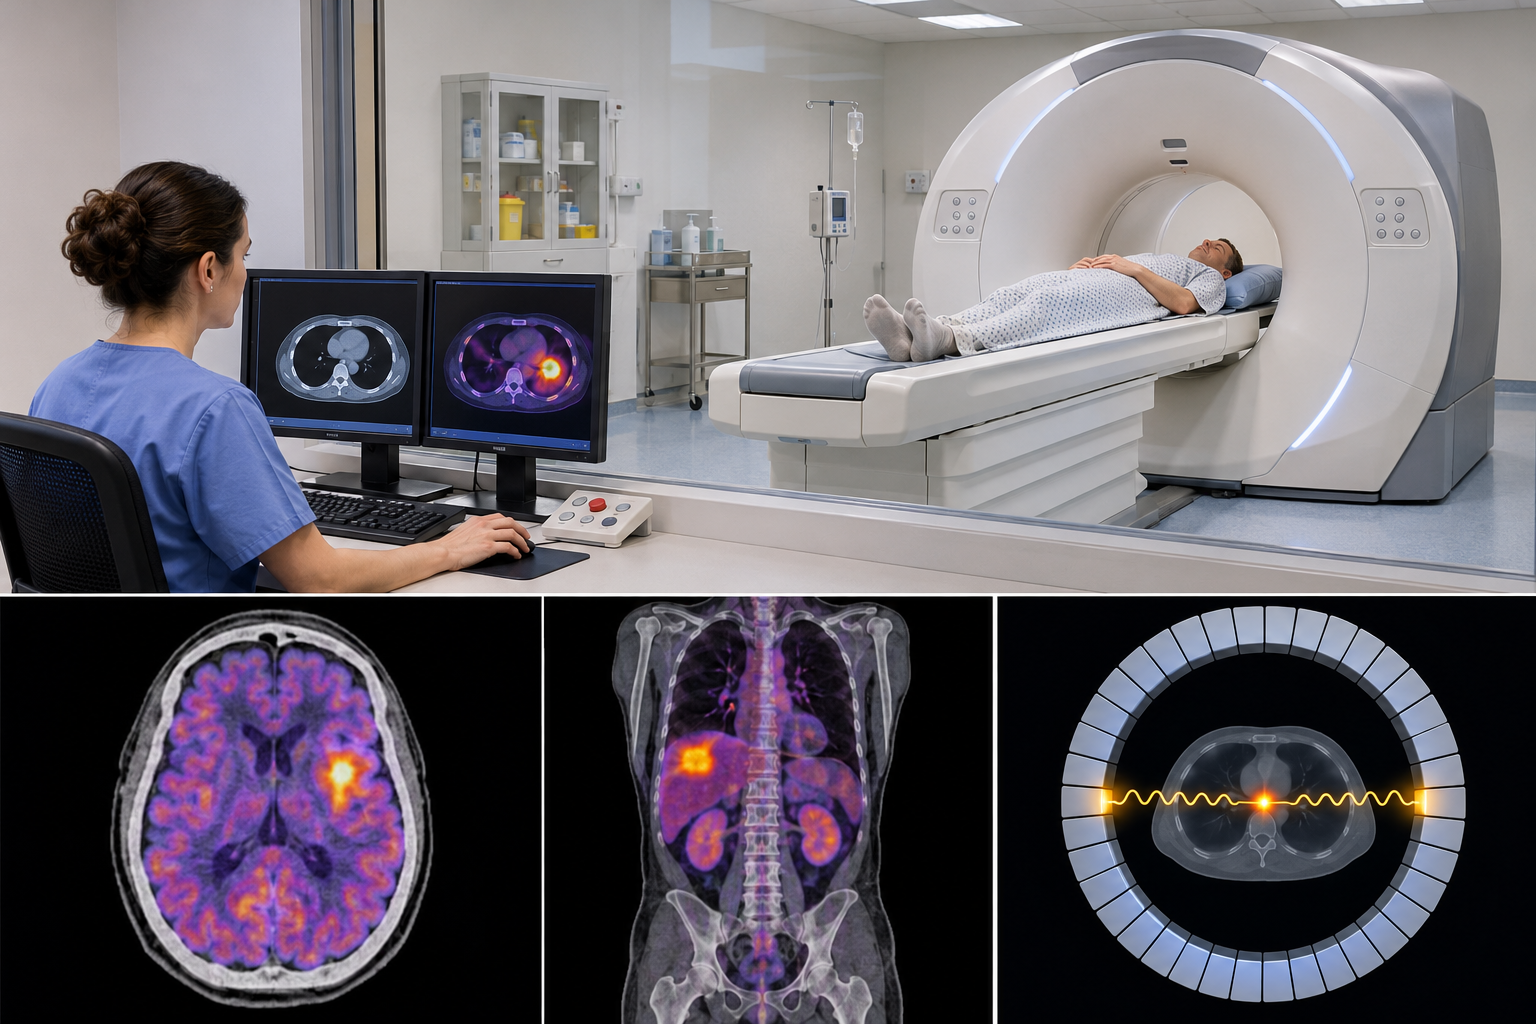
\includegraphics[width=\textwidth,keepaspectratio]{modalities/infographics/pet_realistic.png}
\end{center}
\begin{center}\footnotesize PET localizes paired annihilation photons from positron-emitting tracers to map a selected molecular process; uptake depends on the tracer. AI-generated illustration; PET images are not patient studies.\end{center}

\section{Overview}
Positron Emission Tomography (PET) is a nuclear medicine imaging modality that uses positron-emitting radiopharmaceuticals to visualize metabolic activity, tissue perfusion, molecular transport, receptor expression, and other biochemical processes within the human body.

Unlike CT and conventional MRI, PET can identify molecular and physiological abnormalities before significant anatomical changes become apparent. PET is particularly valuable for cancer staging, treatment response assessment, neurological diseases, myocardial viability, and inflammatory disorders.

This catalogue focuses specifically on PET, PET/CT, and PET/MRI, excluding SPECT and conventional scintigraphy. 

\section{Where PET is used}
The numbered entries summarize reported PET findings and radiopharmaceuticals. Findings depend on the tracer's biological target, acquisition protocol, uptake interval, reconstruction, and clinical context.

\subsection{Neurological and neurodegenerative diseases}
\begin{enumerate}[leftmargin=*,itemsep=0.45em,topsep=0.4em]
\item \textbf{Alzheimer disease.} Useful imaging findings include: Temporoparietal and posterior cingulate hypometabolism. Radiopharmaceutical: ¹⁸F-FDG.
\item \textbf{Alzheimer-associated tau pathology.} Useful imaging findings include: Increased regional tau tracer retention in adults with cognitive impairment being evaluated for Alzheimer disease. Radiopharmaceutical: ¹⁸F-Flortaucipir.
\item \textbf{Amyotrophic lateral sclerosis.} Useful imaging findings include: Altered motor cortical metabolism. Radiopharmaceutical: ¹⁸F-FDG.
\item \textbf{Cerebral amyloid pathology.} Useful imaging findings include: Increased cortical amyloid tracer retention. Radiopharmaceutical: ¹⁸F-Florbetapir.
\item \textbf{Corticobasal syndrome.} Useful imaging findings include: Asymmetric cortical and subcortical hypometabolism. Radiopharmaceutical: ¹⁸F-FDG.
\item \textbf{Creutzfeldt--Jakob disease.} Useful imaging findings include: Regional or widespread cerebral hypometabolism. Radiopharmaceutical: ¹⁸F-FDG.
\item \textbf{Dementia with Lewy bodies.} Useful imaging findings include: Occipital hypometabolism, possible cingulate island sign. Radiopharmaceutical: ¹⁸F-FDG.
\item \textbf{Frontotemporal dementia.} Useful imaging findings include: Frontal and anterior temporal hypometabolism. Radiopharmaceutical: ¹⁸F-FDG.
\item \textbf{Huntington disease.} Useful imaging findings include: Striatal hypometabolism. Radiopharmaceutical: ¹⁸F-FDG.
\item \textbf{Mild cognitive impairment.} Useful imaging findings include: Variable regional hypometabolism. Radiopharmaceutical: ¹⁸F-FDG.
\item \textbf{Multiple system atrophy.} Useful imaging findings include: Putaminal or cerebellar hypometabolism. Radiopharmaceutical: ¹⁸F-FDG.
\item \textbf{Neuroinflammatory disorders.} Useful imaging findings include: Increased tracer binding associated with neuroinflammation in research studies. Radiopharmaceutical: ¹¹C-PK11195.
\item \textbf{Parkinson disease.} Useful imaging findings include: Reduced striatal dopaminergic tracer uptake. Radiopharmaceutical: ¹⁸F-FDOPA.
\item \textbf{Posterior cortical atrophy.} Useful imaging findings include: Posterior cortical hypometabolism. Radiopharmaceutical: ¹⁸F-FDG.
\item \textbf{Primary progressive aphasia.} Useful imaging findings include: Regional language network hypometabolism. Radiopharmaceutical: ¹⁸F-FDG.
\item \textbf{Progressive supranuclear palsy.} Useful imaging findings include: Frontal, thalamic and midbrain hypometabolism. Radiopharmaceutical: ¹⁸F-FDG.
\item \textbf{Spinocerebellar ataxia.} Useful imaging findings include: Cerebellar hypometabolism. Radiopharmaceutical: ¹⁸F-FDG.
\item \textbf{Vascular dementia.} Useful imaging findings include: Multifocal regional metabolic abnormalities. Radiopharmaceutical: ¹⁸F-FDG.
\end{enumerate}

\subsection{Epilepsy}
\begin{enumerate}[leftmargin=*,itemsep=0.45em,topsep=0.4em]
\item \textbf{Drug-resistant focal epilepsy.} Useful imaging findings include: Localized or network-associated hypometabolism. Radiopharmaceutical: ¹⁸F-FDG.
\item \textbf{Focal cortical dysplasia.} Useful imaging findings include: Focal cortical metabolic abnormality. Radiopharmaceutical: ¹⁸F-FDG.
\item \textbf{Frontal lobe epilepsy.} Useful imaging findings include: Regional frontal hypometabolism. Radiopharmaceutical: ¹⁸F-FDG.
\item \textbf{Mesial temporal sclerosis.} Useful imaging findings include: Ipsilateral temporal hypometabolism. Radiopharmaceutical: ¹⁸F-FDG.
\item \textbf{MRI-negative focal epilepsy.} Useful imaging findings include: Potential localization of metabolically abnormal cortex. Radiopharmaceutical: ¹⁸F-FDG.
\item \textbf{Occipital lobe epilepsy.} Useful imaging findings include: Regional occipital hypometabolism. Radiopharmaceutical: ¹⁸F-FDG.
\item \textbf{Parietal lobe epilepsy.} Useful imaging findings include: Regional parietal hypometabolism. Radiopharmaceutical: ¹⁸F-FDG.
\item \textbf{Temporal lobe epilepsy.} Useful imaging findings include: Interictal temporal hypometabolism. Radiopharmaceutical: ¹⁸F-FDG.
\end{enumerate}

\subsection{Brain tumors}
\begin{enumerate}[leftmargin=*,itemsep=0.45em,topsep=0.4em]
\item \textbf{Astrocytoma.} Useful imaging findings include: Variable amino acid tracer uptake. Radiopharmaceutical: ¹⁸F-FET.
\item \textbf{Brain metastases.} Useful imaging findings include: Variable amino acid tracer accumulation. Radiopharmaceutical: ¹⁸F-FET.
\item \textbf{Ependymoma.} Useful imaging findings include: Variable tumor-associated tracer uptake. Radiopharmaceutical: ¹⁸F-FDG.
\item \textbf{Glioblastoma.} Useful imaging findings include: Increased amino acid transport. Radiopharmaceutical: ¹⁸F-FET.
\item \textbf{Medulloblastoma.} Useful imaging findings include: Variable increased glucose metabolism. Radiopharmaceutical: ¹⁸F-FDG.
\item \textbf{Meningioma.} Useful imaging findings include: Increased somatostatin receptor binding. Radiopharmaceutical: ⁶⁸Ga-DOTATATE.
\item \textbf{Oligodendroglioma.} Useful imaging findings include: Increased or variable amino acid uptake. Radiopharmaceutical: ¹¹C-Methionine.
\item \textbf{Primary CNS lymphoma.} Useful imaging findings include: Markedly increased glucose metabolism. Radiopharmaceutical: ¹⁸F-FDG.
\item \textbf{Radiation necrosis.} Useful imaging findings include: Frequently lower amino acid uptake than recurrent tumor, with overlap. Radiopharmaceutical: ¹⁸F-FET.
\item \textbf{Recurrent glioma.} Useful imaging findings include: Increased uptake in viable tumor tissue. Radiopharmaceutical: ¹⁸F-FET.
\item \textbf{Selected residual, recurrent, or MRI-occult pituitary adenoma.} Useful imaging findings include: Focal amino acid tracer uptake may help localize selected lesions; specialized problem-solving application. Radiopharmaceutical: ¹¹C-Methionine.
\item \textbf{Tumor pseudoprogression.} Useful imaging findings include: Variable uptake, potentially distinguishable from progression. Radiopharmaceutical: ¹⁸F-FET.
\end{enumerate}

\subsection{Cerebrovascular diseases}
\begin{enumerate}[leftmargin=*,itemsep=0.45em,topsep=0.4em]
\item \textbf{Carotid artery occlusion.} Useful imaging findings include: Abnormal cerebral perfusion and oxygen extraction. Radiopharmaceutical: ¹⁵O-Oxygen.
\item \textbf{Cerebral infarction.} Useful imaging findings include: Reduced regional glucose metabolism. Radiopharmaceutical: ¹⁸F-FDG.
\item \textbf{Cerebral ischemia.} Useful imaging findings include: Reduced regional cerebral blood flow. Radiopharmaceutical: ¹⁵O-Water.
\item \textbf{Cerebral small vessel disease.} Useful imaging findings include: Regional metabolic or perfusion abnormalities. Radiopharmaceutical: ¹⁸F-FDG.
\item \textbf{Chronic cerebral ischemia.} Useful imaging findings include: Reduced perfusion or increased oxygen extraction. Radiopharmaceutical: ¹⁵O-Water, ¹⁵O-Oxygen.
\item \textbf{Moyamoya disease.} Useful imaging findings include: Reduced cerebral perfusion reserve. Radiopharmaceutical: ¹⁵O-Water.
\end{enumerate}
These are specialized physiological assessments. PET is not a routine first-line imaging modality for acute stroke.

\subsection{Cardiovascular diseases}
\begin{enumerate}[leftmargin=*,itemsep=0.45em,topsep=0.4em]
\item \textbf{Cardiac amyloidosis (research PET).} Useful imaging findings include: Myocardial amyloid tracer retention in investigational studies; not a routine clinical PET test. Radiopharmaceutical: ¹¹C-PiB.
\item \textbf{Cardiac device infection.} Useful imaging findings include: Increased uptake surrounding implanted devices. Radiopharmaceutical: ¹⁸F-FDG.
\item \textbf{Cardiac sarcoidosis.} Useful imaging findings include: Focal or focal-on-diffuse inflammatory myocardial uptake after suppression of physiological myocardial glucose uptake. Radiopharmaceutical: ¹⁸F-FDG.
\item \textbf{Cardiac sympathetic dysfunction.} Useful imaging findings include: Altered sympathetic neuronal tracer uptake. Radiopharmaceutical: ¹¹C-HED.
\item \textbf{Coronary artery disease.} Useful imaging findings include: Stress-induced myocardial perfusion defects. Radiopharmaceutical: ⁸²Rb.
\item \textbf{Coronary microvascular dysfunction.} Useful imaging findings include: Reduced myocardial flow reserve. Radiopharmaceutical: ¹³N-Ammonia.
\item \textbf{Dilated cardiomyopathy.} Useful imaging findings include: Altered myocardial glucose metabolism; perfusion is assessed separately when indicated. Radiopharmaceutical: ¹⁸F-FDG.
\item \textbf{Hibernating myocardium.} Useful imaging findings include: Reduced perfusion with preserved glucose metabolism (perfusion--metabolism mismatch). Radiopharmaceutical: ¹⁸F-FDG with paired perfusion imaging (e.g., ⁸²Rb or ¹³N-ammonia).
\item \textbf{Hypertrophic cardiomyopathy.} Useful imaging findings include: Reduced regional myocardial flow reserve. Radiopharmaceutical: ¹³N-Ammonia.
\item \textbf{Ischemic cardiomyopathy.} Useful imaging findings include: Regional perfusion--metabolism abnormalities assessed with paired imaging. Radiopharmaceutical: ¹⁸F-FDG with a perfusion tracer (e.g., ⁸²Rb or ¹³N-ammonia).
\item \textbf{Multivessel coronary artery disease.} Useful imaging findings include: Reduced absolute myocardial blood flow. Radiopharmaceutical: ⁸²Rb.
\item \textbf{Myocardial ischemia.} Useful imaging findings include: Reversible perfusion defects. Radiopharmaceutical: ¹³N-Ammonia.
\item \textbf{Myocardial scar.} Useful imaging findings include: Matched reduction in perfusion and glucose metabolism. Radiopharmaceutical: ¹⁸F-FDG with paired perfusion imaging (e.g., ⁸²Rb or ¹³N-ammonia).
\item \textbf{Myocarditis.} Useful imaging findings include: Increased inflammatory myocardial uptake in selected cases. Radiopharmaceutical: ¹⁸F-FDG.
\item \textbf{Previous myocardial infarction.} Useful imaging findings include: Fixed perfusion defects. Radiopharmaceutical: ⁸²Rb.
\item \textbf{Prosthetic valve endocarditis.} Useful imaging findings include: Abnormal periprosthetic metabolic uptake. Radiopharmaceutical: ¹⁸F-FDG.
\end{enumerate}
Cardiac FDG studies for sarcoidosis require a dedicated preparation protocol to suppress physiological myocardial uptake; inadequate suppression can make interpretation nonspecific.

\subsection{Vascular and inflammatory arterial diseases}
\begin{enumerate}[leftmargin=*,itemsep=0.45em,topsep=0.4em]
\item \textbf{Active vascular microcalcification.} Useful imaging findings include: Increased uptake within calcifying plaques. Radiopharmaceutical: ¹⁸F-NaF.
\item \textbf{Aortitis.} Useful imaging findings include: Increased aortic wall metabolism. Radiopharmaceutical: ¹⁸F-FDG.
\item \textbf{Atherosclerosis.} Useful imaging findings include: Increased inflammatory plaque activity. Radiopharmaceutical: ¹⁸F-FDG.
\item \textbf{Giant cell arteritis.} Useful imaging findings include: Increased large arterial wall uptake. Radiopharmaceutical: ¹⁸F-FDG.
\item \textbf{Infected aortic aneurysm.} Useful imaging findings include: Increased periaortic inflammatory uptake. Radiopharmaceutical: ¹⁸F-FDG.
\item \textbf{Inflammatory abdominal aortic aneurysm.} Useful imaging findings include: Increased periaortic inflammatory activity. Radiopharmaceutical: ¹⁸F-FDG.
\item \textbf{Takayasu arteritis.} Useful imaging findings include: Increased uptake in inflamed arterial walls. Radiopharmaceutical: ¹⁸F-FDG.
\item \textbf{Vascular graft infection.} Useful imaging findings include: Abnormal graft-associated metabolic activity. Radiopharmaceutical: ¹⁸F-FDG.
\end{enumerate}
Atherosclerotic plaque characterization using PET remains predominantly investigational.

\subsection{Pulmonary and thoracic diseases}
\begin{enumerate}[leftmargin=*,itemsep=0.45em,topsep=0.4em]
\item \textbf{Bronchial carcinoid.} Useful imaging findings include: Increased somatostatin receptor uptake. Radiopharmaceutical: ⁶⁸Ga-DOTATATE.
\item \textbf{Malignant pleural mesothelioma.} Useful imaging findings include: Increased pleural metabolic uptake. Radiopharmaceutical: ¹⁸F-FDG.
\item \textbf{Mediastinal lymphadenopathy.} Useful imaging findings include: Increased nodal metabolism with malignant or inflammatory causes. Radiopharmaceutical: ¹⁸F-FDG.
\item \textbf{Non-small cell lung carcinoma.} Useful imaging findings include: Increased tumor glucose metabolism. Radiopharmaceutical: ¹⁸F-FDG.
\item \textbf{Pulmonary adenocarcinoma.} Useful imaging findings include: Variable increased metabolic activity. Radiopharmaceutical: ¹⁸F-FDG.
\item \textbf{Pulmonary fibrosis.} Useful imaging findings include: Variable uptake in affected lung tissue. Radiopharmaceutical: ¹⁸F-FDG.
\item \textbf{Pulmonary metastases.} Useful imaging findings include: Focal abnormal metabolic activity. Radiopharmaceutical: ¹⁸F-FDG.
\item \textbf{Pulmonary sarcoidosis.} Useful imaging findings include: Increased uptake in active granulomatous lesions. Radiopharmaceutical: ¹⁸F-FDG.
\item \textbf{Pulmonary squamous cell carcinoma.} Useful imaging findings include: Frequently intense glucose metabolism. Radiopharmaceutical: ¹⁸F-FDG.
\item \textbf{Pulmonary tuberculosis.} Useful imaging findings include: Increased uptake in active infectious lesions. Radiopharmaceutical: ¹⁸F-FDG.
\item \textbf{Small cell lung carcinoma.} Useful imaging findings include: Hypermetabolic primary and metastatic lesions. Radiopharmaceutical: ¹⁸F-FDG.
\item \textbf{Solitary pulmonary nodule.} Useful imaging findings include: Variable focal tracer uptake. Radiopharmaceutical: ¹⁸F-FDG.
\item \textbf{Thymic carcinoma.} Useful imaging findings include: Frequently increased glucose metabolism. Radiopharmaceutical: ¹⁸F-FDG.
\item \textbf{Thymoma.} Useful imaging findings include: Variable mediastinal metabolic activity. Radiopharmaceutical: ¹⁸F-FDG.
\end{enumerate}

\subsection{Hematological malignancies}
\begin{enumerate}[leftmargin=*,itemsep=0.45em,topsep=0.4em]
\item \textbf{Anaplastic large cell lymphoma.} Useful imaging findings include: Hypermetabolic nodal or extranodal lesions. Radiopharmaceutical: ¹⁸F-FDG.
\item \textbf{Burkitt lymphoma.} Useful imaging findings include: Markedly increased metabolic activity. Radiopharmaceutical: ¹⁸F-FDG.
\item \textbf{Diffuse large B-cell lymphoma.} Useful imaging findings include: Intense metabolic uptake. Radiopharmaceutical: ¹⁸F-FDG.
\item \textbf{Extramedullary plasmacytoma.} Useful imaging findings include: Hypermetabolic soft-tissue lesions. Radiopharmaceutical: ¹⁸F-FDG.
\item \textbf{Extranodal NK/T-cell lymphoma.} Useful imaging findings include: Increased extranodal metabolic uptake. Radiopharmaceutical: ¹⁸F-FDG.
\item \textbf{Follicular lymphoma.} Useful imaging findings include: Increased nodal metabolic activity. Radiopharmaceutical: ¹⁸F-FDG.
\item \textbf{Hodgkin lymphoma.} Useful imaging findings include: Hypermetabolic nodal and extranodal lesions. Radiopharmaceutical: ¹⁸F-FDG.
\item \textbf{Mantle cell lymphoma.} Useful imaging findings include: Variable increased metabolic uptake. Radiopharmaceutical: ¹⁸F-FDG.
\item \textbf{Marginal zone lymphoma.} Useful imaging findings include: Variable FDG avidity. Radiopharmaceutical: ¹⁸F-FDG.
\item \textbf{Multiple myeloma.} Useful imaging findings include: Metabolically active skeletal or marrow lesions. Radiopharmaceutical: ¹⁸F-FDG.
\item \textbf{Myeloid sarcoma.} Useful imaging findings include: Increased metabolic activity within extramedullary lesions. Radiopharmaceutical: ¹⁸F-FDG.
\item \textbf{Peripheral T-cell lymphoma.} Useful imaging findings include: Increased metabolic activity. Radiopharmaceutical: ¹⁸F-FDG.
\item \textbf{Primary cutaneous lymphoma.} Useful imaging findings include: Variable cutaneous metabolic uptake. Radiopharmaceutical: ¹⁸F-FDG.
\item \textbf{Primary mediastinal B-cell lymphoma.} Useful imaging findings include: Intense mediastinal metabolic activity. Radiopharmaceutical: ¹⁸F-FDG.
\item \textbf{Richter transformation.} Useful imaging findings include: Increased metabolic activity in suspicious lesions. Radiopharmaceutical: ¹⁸F-FDG.
\item \textbf{Solitary plasmacytoma.} Useful imaging findings include: Focal increased metabolic activity. Radiopharmaceutical: ¹⁸F-FDG.
\end{enumerate}

\subsection{Head and neck malignancies}
\begin{enumerate}[leftmargin=*,itemsep=0.45em,topsep=0.4em]
\item \textbf{Adenoid cystic carcinoma.} Useful imaging findings include: Variable metabolic activity. Radiopharmaceutical: ¹⁸F-FDG.
\item \textbf{Cervical nodal metastases.} Useful imaging findings include: Increased regional lymph node metabolism. Radiopharmaceutical: ¹⁸F-FDG.
\item \textbf{Esthesioneuroblastoma.} Useful imaging findings include: Increased tumor metabolism or receptor-specific uptake. Radiopharmaceutical: ¹⁸F-FDG, ⁶⁸Ga-DOTATATE.
\item \textbf{Head and neck cancer of unknown primary.} Useful imaging findings include: Potential localization of occult primary tumor. Radiopharmaceutical: ¹⁸F-FDG.
\item \textbf{Hypopharyngeal carcinoma.} Useful imaging findings include: Increased regional metabolic activity. Radiopharmaceutical: ¹⁸F-FDG.
\item \textbf{Laryngeal carcinoma.} Useful imaging findings include: Hypermetabolic laryngeal lesion. Radiopharmaceutical: ¹⁸F-FDG.
\item \textbf{Nasopharyngeal carcinoma.} Useful imaging findings include: Increased nasopharyngeal and nodal uptake. Radiopharmaceutical: ¹⁸F-FDG.
\item \textbf{Oral squamous cell carcinoma.} Useful imaging findings include: Increased tumor metabolic activity. Radiopharmaceutical: ¹⁸F-FDG.
\item \textbf{Oropharyngeal carcinoma.} Useful imaging findings include: Increased primary and nodal metabolic uptake. Radiopharmaceutical: ¹⁸F-FDG.
\item \textbf{Salivary gland carcinoma.} Useful imaging findings include: Variable tumor-associated metabolic uptake. Radiopharmaceutical: ¹⁸F-FDG.
\item \textbf{Sinonasal carcinoma.} Useful imaging findings include: Increased tumor glucose metabolism. Radiopharmaceutical: ¹⁸F-FDG.
\item \textbf{Tongue carcinoma.} Useful imaging findings include: Focal hypermetabolic lesion. Radiopharmaceutical: ¹⁸F-FDG.
\end{enumerate}

\subsection{Thyroid and parathyroid diseases}
\begin{enumerate}[leftmargin=*,itemsep=0.45em,topsep=0.4em]
\item \textbf{Anaplastic thyroid carcinoma.} Useful imaging findings include: Frequently intense glucose metabolism. Radiopharmaceutical: ¹⁸F-FDG.
\item \textbf{Ectopic parathyroid adenoma.} Useful imaging findings include: Abnormal uptake outside expected gland location. Radiopharmaceutical: ¹⁸F-Fluorocholine.
\item \textbf{Follicular thyroid carcinoma.} Useful imaging findings include: Variable metabolic activity. Radiopharmaceutical: ¹⁸F-FDG.
\item \textbf{Medullary thyroid carcinoma.} Useful imaging findings include: Increased amino acid tracer uptake. Radiopharmaceutical: ¹⁸F-FDOPA.
\item \textbf{Papillary thyroid carcinoma.} Useful imaging findings include: Increased uptake in selected non-iodine-avid lesions. Radiopharmaceutical: ¹⁸F-FDG.
\item \textbf{Parathyroid adenoma.} Useful imaging findings include: Focal fluorocholine uptake. Radiopharmaceutical: ¹⁸F-Fluorocholine.
\item \textbf{Parathyroid hyperplasia.} Useful imaging findings include: Increased uptake in hyperfunctioning glands. Radiopharmaceutical: ¹⁸F-Fluorocholine.
\item \textbf{Radioiodine-refractory thyroid carcinoma.} Useful imaging findings include: Metabolically active residual or metastatic lesions. Radiopharmaceutical: ¹⁸F-FDG.
\end{enumerate}

\subsection{Breast diseases}
\begin{enumerate}[leftmargin=*,itemsep=0.45em,topsep=0.4em]
\item \textbf{HER2-positive breast cancer.} Useful imaging findings include: Variable increased glucose metabolism. Radiopharmaceutical: ¹⁸F-FDG.
\item \textbf{Inflammatory breast cancer.} Useful imaging findings include: Diffuse breast and skin metabolic uptake. Radiopharmaceutical: ¹⁸F-FDG.
\item \textbf{Invasive ductal carcinoma.} Useful imaging findings include: Increased tumor glucose metabolism. Radiopharmaceutical: ¹⁸F-FDG.
\item \textbf{Invasive lobular carcinoma.} Useful imaging findings include: Variable or relatively low FDG uptake. Radiopharmaceutical: ¹⁸F-FDG.
\item \textbf{Metastatic breast carcinoma.} Useful imaging findings include: Abnormal uptake in metastatic sites; FES can assess estrogen receptor status in selected cases. Radiopharmaceutical: ¹⁸F-FDG; ¹⁸F-FES as an adjunct to biopsy when indicated.
\item \textbf{Recurrent breast carcinoma.} Useful imaging findings include: Increased uptake within recurrent lesions. Radiopharmaceutical: ¹⁸F-FDG.
\item \textbf{Recurrent or metastatic breast cancer with uncertain estrogen receptor status.} Useful imaging findings include: Estrogen receptor-positive lesions may be detected; FES PET is an adjunct to, not a replacement for, biopsy. Radiopharmaceutical: ¹⁸F-FES.
\item \textbf{Triple-negative breast cancer.} Useful imaging findings include: Frequently increased glucose metabolism. Radiopharmaceutical: ¹⁸F-FDG.
\end{enumerate}
PET is not a replacement for screening mammography or diagnostic breast biopsy.

\subsection{Gastrointestinal malignancies}
\begin{enumerate}[leftmargin=*,itemsep=0.45em,topsep=0.4em]
\item \textbf{Anal squamous cell carcinoma.} Useful imaging findings include: Increased primary and nodal uptake. Radiopharmaceutical: ¹⁸F-FDG.
\item \textbf{Appendiceal carcinoma.} Useful imaging findings include: Variable metabolic uptake. Radiopharmaceutical: ¹⁸F-FDG.
\item \textbf{Colorectal carcinoma.} Useful imaging findings include: Hypermetabolic primary or recurrent lesions. Radiopharmaceutical: ¹⁸F-FDG.
\item \textbf{Esophageal adenocarcinoma.} Useful imaging findings include: Increased tumor glucose metabolism. Radiopharmaceutical: ¹⁸F-FDG.
\item \textbf{Esophageal squamous cell carcinoma.} Useful imaging findings include: Frequently intense metabolic activity. Radiopharmaceutical: ¹⁸F-FDG.
\item \textbf{Gastric adenocarcinoma.} Useful imaging findings include: Variable metabolic activity. Radiopharmaceutical: ¹⁸F-FDG.
\item \textbf{Gastrointestinal lymphoma.} Useful imaging findings include: Variable or intense metabolic uptake. Radiopharmaceutical: ¹⁸F-FDG.
\item \textbf{Gastrointestinal stromal tumor.} Useful imaging findings include: Increased metabolic uptake in active tumors. Radiopharmaceutical: ¹⁸F-FDG.
\item \textbf{Peritoneal carcinomatosis.} Useful imaging findings include: Hypermetabolic peritoneal deposits. Radiopharmaceutical: ¹⁸F-FDG.
\item \textbf{Rectal carcinoma.} Useful imaging findings include: Increased uptake within viable tumor. Radiopharmaceutical: ¹⁸F-FDG.
\item \textbf{Recurrent colorectal carcinoma.} Useful imaging findings include: Increased metabolic activity at recurrence sites. Radiopharmaceutical: ¹⁸F-FDG.
\item \textbf{Small bowel adenocarcinoma.} Useful imaging findings include: Increased tumor metabolic activity. Radiopharmaceutical: ¹⁸F-FDG.
\end{enumerate}

\subsection{Liver, biliary and pancreatic malignancies}
\begin{enumerate}[leftmargin=*,itemsep=0.45em,topsep=0.4em]
\item \textbf{Extrahepatic cholangiocarcinoma.} Useful imaging findings include: Variable increased biliary tumor uptake. Radiopharmaceutical: ¹⁸F-FDG.
\item \textbf{Gallbladder carcinoma.} Useful imaging findings include: Increased tumor-associated metabolism. Radiopharmaceutical: ¹⁸F-FDG.
\item \textbf{Hepatic metastases.} Useful imaging findings include: Focal abnormal metabolic activity. Radiopharmaceutical: ¹⁸F-FDG.
\item \textbf{Hepatic neuroendocrine metastases.} Useful imaging findings include: Increased receptor-specific uptake. Radiopharmaceutical: ⁶⁸Ga-DOTATATE.
\item \textbf{Hepatocellular carcinoma.} Useful imaging findings include: Variable glucose metabolism depending on tumor differentiation. Radiopharmaceutical: ¹⁸F-FDG.
\item \textbf{Intrahepatic cholangiocarcinoma.} Useful imaging findings include: Increased metabolic uptake in many lesions. Radiopharmaceutical: ¹⁸F-FDG.
\item \textbf{Pancreatic acinar cell carcinoma.} Useful imaging findings include: Variable metabolic uptake. Radiopharmaceutical: ¹⁸F-FDG.
\item \textbf{Pancreatic ductal adenocarcinoma.} Useful imaging findings include: Increased pancreatic tumor metabolism. Radiopharmaceutical: ¹⁸F-FDG.
\item \textbf{Pancreatic neuroendocrine tumor.} Useful imaging findings include: Increased somatostatin receptor binding. Radiopharmaceutical: ⁶⁸Ga-DOTATATE.
\item \textbf{Recurrent pancreatic carcinoma.} Useful imaging findings include: Abnormal metabolic uptake at recurrence sites. Radiopharmaceutical: ¹⁸F-FDG.
\end{enumerate}

\subsection{Neuroendocrine and adrenal tumors}
\begin{enumerate}[leftmargin=*,itemsep=0.45em,topsep=0.4em]
\item \textbf{Adrenocortical carcinoma.} Useful imaging findings include: Increased glucose metabolism. Radiopharmaceutical: ¹⁸F-FDG.
\item \textbf{Bronchial carcinoid.} Useful imaging findings include: Increased somatostatin receptor tracer uptake. Radiopharmaceutical: ⁶⁸Ga-DOTATATE.
\item \textbf{Gastrinoma.} Useful imaging findings include: Increased somatostatin receptor uptake. Radiopharmaceutical: ⁶⁸Ga-DOTATATE.
\item \textbf{Gastroenteropancreatic neuroendocrine tumor.} Useful imaging findings include: Increased somatostatin receptor expression. Radiopharmaceutical: ⁶⁸Ga-DOTATATE.
\item \textbf{Glucagonoma.} Useful imaging findings include: Increased somatostatin receptor uptake. Radiopharmaceutical: ⁶⁸Ga-DOTATATE.
\item \textbf{Insulinoma.} Useful imaging findings include: Increased GLP-1 receptor tracer uptake in selected tumors. Radiopharmaceutical: ⁶⁸Ga-Exendin.
\item \textbf{Merkel cell carcinoma.} Useful imaging findings include: Increased tumor glucose metabolism. Radiopharmaceutical: ¹⁸F-FDG.
\item \textbf{Neuroblastoma.} Useful imaging findings include: Variable amino acid or glucose metabolic uptake. Radiopharmaceutical: ¹⁸F-FDOPA, ¹⁸F-FDG.
\item \textbf{Paraganglioma.} Useful imaging findings include: Frequently intense somatostatin receptor uptake. Radiopharmaceutical: ⁶⁸Ga-DOTATATE.
\item \textbf{Pheochromocytoma.} Useful imaging findings include: Increased receptor-specific or amino acid tracer uptake. Radiopharmaceutical: ⁶⁸Ga-DOTATATE, ¹⁸F-FDOPA.
\item \textbf{Poorly differentiated neuroendocrine carcinoma.} Useful imaging findings include: Frequently intense glucose metabolism. Radiopharmaceutical: ¹⁸F-FDG.
\item \textbf{Small bowel neuroendocrine tumor.} Useful imaging findings include: Receptor-positive primary and metastatic lesions. Radiopharmaceutical: ⁶⁸Ga-DOTATATE.
\item \textbf{VIPoma.} Useful imaging findings include: Increased somatostatin receptor uptake. Radiopharmaceutical: ⁶⁸Ga-DOTATATE.
\item \textbf{Well-differentiated neuroendocrine tumor.} Useful imaging findings include: Increased receptor-specific uptake. Radiopharmaceutical: ⁶⁴Cu-DOTATATE.
\end{enumerate}

\subsection{Male reproductive and urinary malignancies}
\begin{enumerate}[leftmargin=*,itemsep=0.45em,topsep=0.4em]
\item \textbf{Biochemically recurrent prostate cancer.} Useful imaging findings include: PSMA-positive recurrent or metastatic lesions. Radiopharmaceutical: ¹⁸F-DCFPyL.
\item \textbf{Bladder urothelial carcinoma.} Useful imaging findings include: Increased uptake in selected primary or metastatic lesions. Radiopharmaceutical: ¹⁸F-FDG.
\item \textbf{Metastatic castration-resistant prostate cancer.} Useful imaging findings include: Variable PSMA expression in metastatic lesions. Radiopharmaceutical: ⁶⁸Ga-PSMA-11.
\item \textbf{Neuroendocrine prostate carcinoma.} Useful imaging findings include: Increased FDG uptake with potentially reduced PSMA expression. Radiopharmaceutical: ¹⁸F-FDG.
\item \textbf{Penile squamous cell carcinoma.} Useful imaging findings include: Increased primary or metastatic uptake. Radiopharmaceutical: ¹⁸F-FDG.
\item \textbf{Prostate adenocarcinoma.} Useful imaging findings include: Increased PSMA-targeted tracer uptake. Radiopharmaceutical: ⁶⁸Ga-PSMA-11.
\item \textbf{Renal cell carcinoma.} Useful imaging findings include: Variable uptake, particularly in metastatic disease. Radiopharmaceutical: ¹⁸F-FDG.
\item \textbf{Renal lymphoma.} Useful imaging findings include: Markedly increased metabolic activity. Radiopharmaceutical: ¹⁸F-FDG.
\item \textbf{Testicular seminoma.} Useful imaging findings include: Increased uptake in selected residual tumor masses. Radiopharmaceutical: ¹⁸F-FDG.
\item \textbf{Upper urinary tract urothelial carcinoma.} Useful imaging findings include: Variable metabolic activity. Radiopharmaceutical: ¹⁸F-FDG.
\end{enumerate}

\subsection{Female reproductive malignancies}
\begin{enumerate}[leftmargin=*,itemsep=0.45em,topsep=0.4em]
\item \textbf{Cervical carcinoma.} Useful imaging findings include: Increased cervical and metastatic metabolic uptake. Radiopharmaceutical: ¹⁸F-FDG.
\item \textbf{Endometrial carcinoma.} Useful imaging findings include: Increased uterine or metastatic metabolic activity. Radiopharmaceutical: ¹⁸F-FDG.
\item \textbf{Endometrial stromal sarcoma.} Useful imaging findings include: Variable metabolic uptake. Radiopharmaceutical: ¹⁸F-FDG.
\item \textbf{Fallopian tube carcinoma.} Useful imaging findings include: Increased tumor-associated uptake. Radiopharmaceutical: ¹⁸F-FDG.
\item \textbf{Ovarian epithelial carcinoma.} Useful imaging findings include: Hypermetabolic pelvic and peritoneal lesions. Radiopharmaceutical: ¹⁸F-FDG.
\item \textbf{Primary peritoneal carcinoma.} Useful imaging findings include: Hypermetabolic peritoneal deposits. Radiopharmaceutical: ¹⁸F-FDG.
\item \textbf{Recurrent ovarian carcinoma.} Useful imaging findings include: Increased metabolic activity within recurrent lesions. Radiopharmaceutical: ¹⁸F-FDG.
\item \textbf{Uterine leiomyosarcoma.} Useful imaging findings include: Frequently increased glucose metabolism. Radiopharmaceutical: ¹⁸F-FDG.
\item \textbf{Vaginal carcinoma.} Useful imaging findings include: Increased tumor-associated metabolic activity. Radiopharmaceutical: ¹⁸F-FDG.
\item \textbf{Vulvar carcinoma.} Useful imaging findings include: Increased primary and nodal metabolic uptake. Radiopharmaceutical: ¹⁸F-FDG.
\end{enumerate}

\subsection{Bone and soft-tissue tumors}
\begin{enumerate}[leftmargin=*,itemsep=0.45em,topsep=0.4em]
\item \textbf{Angiosarcoma.} Useful imaging findings include: Variable increased metabolic uptake. Radiopharmaceutical: ¹⁸F-FDG.
\item \textbf{Bone lymphoma.} Useful imaging findings include: Markedly increased skeletal metabolic activity. Radiopharmaceutical: ¹⁸F-FDG.
\item \textbf{Chondrosarcoma.} Useful imaging findings include: Variable metabolic uptake depending on tumor grade. Radiopharmaceutical: ¹⁸F-FDG.
\item \textbf{Chordoma.} Useful imaging findings include: Variable metabolic activity. Radiopharmaceutical: ¹⁸F-FDG.
\item \textbf{Desmoid-type fibromatosis.} Useful imaging findings include: Variable metabolic activity. Radiopharmaceutical: ¹⁸F-FDG.
\item \textbf{Ewing sarcoma.} Useful imaging findings include: Frequently intense metabolic uptake. Radiopharmaceutical: ¹⁸F-FDG.
\item \textbf{Giant cell tumor of bone.} Useful imaging findings include: Frequently intense uptake despite benign or intermediate pathology. Radiopharmaceutical: ¹⁸F-FDG.
\item \textbf{Leiomyosarcoma.} Useful imaging findings include: Increased glucose metabolism in viable tumor. Radiopharmaceutical: ¹⁸F-FDG.
\item \textbf{Liposarcoma.} Useful imaging findings include: Variable uptake depending on histological subtype. Radiopharmaceutical: ¹⁸F-FDG.
\item \textbf{Malignant peripheral nerve sheath tumor.} Useful imaging findings include: Frequently increased metabolic activity. Radiopharmaceutical: ¹⁸F-FDG.
\item \textbf{Osteoblastic bone metastases.} Useful imaging findings include: Increased skeletal mineral turnover. Radiopharmaceutical: ¹⁸F-NaF.
\item \textbf{Osteolytic bone metastases.} Useful imaging findings include: Increased metabolism in viable tumor. Radiopharmaceutical: ¹⁸F-FDG.
\item \textbf{Osteosarcoma.} Useful imaging findings include: Increased tumor glucose metabolism. Radiopharmaceutical: ¹⁸F-FDG.
\item \textbf{Rhabdomyosarcoma.} Useful imaging findings include: Increased metabolic activity. Radiopharmaceutical: ¹⁸F-FDG.
\item \textbf{Synovial sarcoma.} Useful imaging findings include: Increased tumor-associated metabolic activity. Radiopharmaceutical: ¹⁸F-FDG.
\item \textbf{Undifferentiated pleomorphic sarcoma.} Useful imaging findings include: Increased tumor glucose metabolism. Radiopharmaceutical: ¹⁸F-FDG.
\end{enumerate}

\subsection{Skin malignancies}
\begin{enumerate}[leftmargin=*,itemsep=0.45em,topsep=0.4em]
\item \textbf{Cutaneous lymphoma.} Useful imaging findings include: Variable increased cutaneous metabolic uptake. Radiopharmaceutical: ¹⁸F-FDG.
\item \textbf{Cutaneous squamous cell carcinoma.} Useful imaging findings include: Increased metabolic uptake in advanced disease. Radiopharmaceutical: ¹⁸F-FDG.
\item \textbf{Dermatofibrosarcoma protuberans.} Useful imaging findings include: Variable tumor metabolic activity. Radiopharmaceutical: ¹⁸F-FDG.
\item \textbf{Malignant melanoma.} Useful imaging findings include: Hypermetabolic primary or metastatic lesions. Radiopharmaceutical: ¹⁸F-FDG.
\item \textbf{Merkel cell carcinoma.} Useful imaging findings include: Frequently intense metabolic activity. Radiopharmaceutical: ¹⁸F-FDG.
\end{enumerate}

\subsection{Infectious diseases}
\begin{enumerate}[leftmargin=*,itemsep=0.45em,topsep=0.4em]
\item \textbf{Acute osteomyelitis.} Useful imaging findings include: Increased osseous inflammatory metabolism. Radiopharmaceutical: ¹⁸F-FDG.
\item \textbf{Chronic osteomyelitis.} Useful imaging findings include: Persistent focal skeletal metabolic activity. Radiopharmaceutical: ¹⁸F-FDG.
\item \textbf{Diabetic foot osteomyelitis.} Useful imaging findings include: Increased osseous inflammatory uptake. Radiopharmaceutical: ¹⁸F-FDG.
\item \textbf{Disseminated infection.} Useful imaging findings include: Multiple abnormal inflammatory foci. Radiopharmaceutical: ¹⁸F-FDG.
\item \textbf{Fever of unknown origin.} Useful imaging findings include: Localization of abnormal metabolic foci. Radiopharmaceutical: ¹⁸F-FDG.
\item \textbf{Fungal infection.} Useful imaging findings include: Increased metabolic activity in affected tissues. Radiopharmaceutical: ¹⁸F-FDG.
\item \textbf{Hepatic abscess.} Useful imaging findings include: Increased inflammatory uptake, often peripheral. Radiopharmaceutical: ¹⁸F-FDG.
\item \textbf{Infected hepatic cyst.} Useful imaging findings include: Increased cyst-associated inflammatory uptake. Radiopharmaceutical: ¹⁸F-FDG.
\item \textbf{Infected orthopedic hardware.} Useful imaging findings include: Increased peri-implant metabolic activity. Radiopharmaceutical: ¹⁸F-FDG.
\item \textbf{Infected renal cyst.} Useful imaging findings include: Increased cyst wall metabolic activity. Radiopharmaceutical: ¹⁸F-FDG.
\item \textbf{Intra-abdominal abscess.} Useful imaging findings include: Focal inflammatory metabolic uptake. Radiopharmaceutical: ¹⁸F-FDG.
\item \textbf{Prosthetic joint infection.} Useful imaging findings include: Abnormal periprosthetic uptake, with limited specificity. Radiopharmaceutical: ¹⁸F-FDG.
\item \textbf{Septic emboli.} Useful imaging findings include: Multifocal inflammatory metabolic abnormalities. Radiopharmaceutical: ¹⁸F-FDG.
\item \textbf{Spondylodiscitis.} Useful imaging findings include: Increased uptake involving disc and adjacent vertebral structures. Radiopharmaceutical: ¹⁸F-FDG.
\item \textbf{Tuberculosis.} Useful imaging findings include: Hypermetabolic infectious lesions. Radiopharmaceutical: ¹⁸F-FDG.
\item \textbf{Vertebral osteomyelitis.} Useful imaging findings include: Increased vertebral uptake. Radiopharmaceutical: ¹⁸F-FDG.
\end{enumerate}

\subsection{Autoimmune and systemic inflammatory diseases}
\begin{enumerate}[leftmargin=*,itemsep=0.45em,topsep=0.4em]
\item \textbf{Autoimmune pancreatitis.} Useful imaging findings include: Diffuse or focal pancreatic metabolic uptake. Radiopharmaceutical: ¹⁸F-FDG.
\item \textbf{Crohn disease.} Useful imaging findings include: Increased inflammatory bowel wall metabolism. Radiopharmaceutical: ¹⁸F-FDG.
\item \textbf{Dermatomyositis.} Useful imaging findings include: Increased muscle-associated inflammatory uptake in some cases. Radiopharmaceutical: ¹⁸F-FDG.
\item \textbf{IgG4-related disease.} Useful imaging findings include: Multiorgan inflammatory metabolic uptake. Radiopharmaceutical: ¹⁸F-FDG.
\item \textbf{Polymyalgia rheumatica.} Useful imaging findings include: Characteristic periarticular inflammatory uptake. Radiopharmaceutical: ¹⁸F-FDG.
\item \textbf{Polymyositis.} Useful imaging findings include: Increased muscle metabolism in active inflammation. Radiopharmaceutical: ¹⁸F-FDG.
\item \textbf{Psoriatic arthritis.} Useful imaging findings include: Increased joint or entheseal inflammatory activity. Radiopharmaceutical: ¹⁸F-FDG.
\item \textbf{Relapsing polychondritis.} Useful imaging findings include: Increased uptake in inflamed cartilaginous structures. Radiopharmaceutical: ¹⁸F-FDG.
\item \textbf{Retroperitoneal fibrosis.} Useful imaging findings include: Increased metabolic activity in active fibrotic tissue. Radiopharmaceutical: ¹⁸F-FDG.
\item \textbf{Rheumatoid arthritis.} Useful imaging findings include: Increased synovial metabolic activity. Radiopharmaceutical: ¹⁸F-FDG.
\item \textbf{Systemic sarcoidosis.} Useful imaging findings include: Hypermetabolic granulomatous lesions. Radiopharmaceutical: ¹⁸F-FDG.
\item \textbf{Ulcerative colitis.} Useful imaging findings include: Increased colonic inflammatory uptake. Radiopharmaceutical: ¹⁸F-FDG.
\end{enumerate}

\subsection{Nonmalignant skeletal disorders}
\begin{enumerate}[leftmargin=*,itemsep=0.45em,topsep=0.4em]
\item \textbf{Aseptic prosthetic loosening.} Useful imaging findings include: Increased periprosthetic bone remodeling. Radiopharmaceutical: ¹⁸F-NaF.
\item \textbf{Fibrous dysplasia.} Useful imaging findings include: Increased skeletal remodeling activity. Radiopharmaceutical: ¹⁸F-NaF.
\item \textbf{Heterotopic ossification.} Useful imaging findings include: Increased extraosseous mineralization. Radiopharmaceutical: ¹⁸F-NaF.
\item \textbf{Insufficiency fracture.} Useful imaging findings include: Increased tracer uptake at fracture sites. Radiopharmaceutical: ¹⁸F-NaF.
\item \textbf{Osteoarthritis.} Useful imaging findings include: Increased subchondral bone turnover. Radiopharmaceutical: ¹⁸F-NaF.
\item \textbf{Osteonecrosis.} Useful imaging findings include: Variable regional skeletal tracer uptake. Radiopharmaceutical: ¹⁸F-NaF.
\item \textbf{Paget disease of bone.} Useful imaging findings include: Intense skeletal mineral turnover. Radiopharmaceutical: ¹⁸F-NaF.
\item \textbf{Stress fracture.} Useful imaging findings include: Focal increased bone remodeling. Radiopharmaceutical: ¹⁸F-NaF.
\end{enumerate}

\subsection{Summary of catalogue}
\begin{center}
\begin{tabular}{@{}p{0.70\textwidth}r@{}}
\toprule
\textbf{Disease category} & \textbf{Entries} \\
\midrule
Autoimmune and systemic inflammatory diseases & 12 \\
Bone and soft-tissue tumors & 16 \\
Brain tumors & 12 \\
Breast diseases & 8 \\
Cardiovascular diseases & 16 \\
Cerebrovascular diseases & 6 \\
Epilepsy & 8 \\
Female reproductive malignancies & 10 \\
Gastrointestinal malignancies & 12 \\
Head and neck malignancies & 12 \\
Hematological malignancies & 16 \\
Infectious diseases & 16 \\
Liver, biliary and pancreatic malignancies & 10 \\
Male reproductive and urinary malignancies & 10 \\
Neuroendocrine and adrenal tumors & 14 \\
Neurological and neurodegenerative diseases & 18 \\
Nonmalignant skeletal disorders & 8 \\
Pulmonary and thoracic diseases & 14 \\
Skin malignancies & 5 \\
Thyroid and parathyroid diseases & 8 \\
Vascular and inflammatory arterial diseases & 8 \\
\midrule
\textbf{Total} & \textbf{239} \\
\bottomrule
\end{tabular}
\end{center}

\subsection{Major PET radiopharmaceuticals}
PET is a molecular imaging platform; different radiopharmaceuticals examine different biochemical and physiological processes.
\begin{longtable}{@{}p{0.27\textwidth}p{0.36\textwidth}p{0.29\textwidth}@{}}
\toprule
\textbf{Radiopharmaceutical} & \textbf{Molecular target or biological process} & \textbf{Primary application} \\
\midrule
\endfirsthead
\toprule
\textbf{Radiopharmaceutical} & \textbf{Molecular target or biological process} & \textbf{Primary application} \\
\midrule
\endhead
¹³N-Ammonia & Myocardial perfusion & Cardiology \\
¹¹C-Choline & Choline metabolism & Prostate cancer \\
¹¹C-HED & Sympathetic neuronal transport & Cardiac innervation \\
¹¹C-Methionine & Amino acid transport & Brain tumors \\
¹¹C-PiB & Amyloid plaques & Amyloid imaging \\
¹¹C-PK11195 & Translocator protein (TSPO) & Neuroinflammation research \\
¹¹C-Raclopride & Dopamine D2/D3 receptors & Neuroscience research \\
¹⁵O-Oxygen & Oxygen metabolism & Cerebral physiological assessment \\
¹⁵O-Water & Tissue perfusion & Quantitative blood flow imaging \\
¹⁸F-DCFPyL & PSMA expression & Prostate cancer \\
¹⁸F-FAZA & Tissue hypoxia & Investigational tumor imaging \\
¹⁸F-FDG & Glucose metabolism & Oncology, neurology, inflammation \\
¹⁸F-FDOPA & Amino acid transport and decarboxylation & Neurology and neuroendocrine tumors \\
¹⁸F-FES & Estrogen receptor expression & Breast cancer \\
¹⁸F-FET & Amino acid transport & Brain tumors \\
¹⁸F-Florbetaben & Amyloid plaques & Alzheimer-associated pathology \\
¹⁸F-Florbetapir & Amyloid plaques & Alzheimer-associated pathology \\
¹⁸F-Flortaucipir & Aggregated tau neurofibrillary tangles & Alzheimer disease assessment in selected adults with cognitive impairment \\
¹⁸F-FLT & Thymidine metabolism and proliferation & Investigational tumor imaging \\
¹⁸F-Fluciclovine & Amino acid transport & Recurrent prostate cancer \\
¹⁸F-Fluorocholine & Choline metabolism & Parathyroid and selected tumor imaging \\
¹⁸F-Flutemetamol & Amyloid plaques & Alzheimer-associated pathology \\
¹⁸F-FMISO & Tissue hypoxia & Investigational tumor hypoxia imaging \\
¹⁸F-NaF & Bone mineral turnover & Skeletal imaging \\
¹⁸F-PSMA-1007 & PSMA expression & Prostate cancer \\
⁶⁴Cu-DOTATATE & Somatostatin receptor expression & Neuroendocrine tumors \\
⁶⁸Ga-DOTANOC & Somatostatin receptor expression & Neuroendocrine tumors \\
⁶⁸Ga-DOTATATE & Somatostatin receptor expression & Neuroendocrine tumors \\
⁶⁸Ga-DOTATOC & Somatostatin receptor expression & Neuroendocrine tumors \\
⁶⁸Ga-Exendin & GLP-1 receptors & Insulinoma localization \\
⁶⁸Ga-FAPI & Fibroblast activation protein & Emerging tumor and fibrosis imaging \\
⁶⁸Ga-PSMA-11 & PSMA expression & Prostate cancer \\
⁸²Rb-Chloride & Myocardial perfusion & Cardiology \\
⁸⁹Zr-Labeled antibodies & Antibody biodistribution & Investigational molecular imaging \\
⁸⁹Zr-Trastuzumab & HER2-targeted antibody distribution & Investigational immuno-PET \\
\bottomrule
\end{longtable}

\subsection{Common PET radionuclides}
\begin{longtable}{@{}p{0.28\textwidth}p{0.20\textwidth}p{0.44\textwidth}@{}}
\toprule
\textbf{Radionuclide} & \textbf{Physical half-life} & \textbf{Common application} \\
\midrule
\endfirsthead
\toprule
Carbon-11 & 20.3 minutes & Molecular and neurological imaging \\
\midrule
\endhead
Copper-64 & 12.7 hours & Receptor-targeted imaging \\
Fluorine-18 & 109.8 minutes & General metabolic and molecular imaging \\
Gallium-68 & 67.7 minutes & Receptor-targeted imaging \\
Iodine-124 & 4.18 days & Thyroid and molecular imaging \\
Nitrogen-13 & 9.97 minutes & Myocardial perfusion \\
Oxygen-15 & 2.04 minutes & Tissue perfusion and oxygen metabolism \\
\textbf{Radionuclide} & \textbf{Physical half-life} & \textbf{Common application} \\
Rubidium-82 & 76 seconds & Myocardial perfusion \\
Yttrium-90 & 64.1 hours & Post-radioembolization PET dosimetry \\
Zirconium-89 & 78.4 hours & Antibody-based molecular imaging \\
\bottomrule
\end{longtable}

\subsection{Physical principles of PET}
PET is based on positron emission followed by electron--positron annihilation. A positron interacts with an electron, producing predominantly two annihilation photons of approximately 511 keV traveling in nearly opposite directions:
\begin{equation}
e^{+}+e^{-}\rightarrow 2\gamma.
\end{equation}
Photon energy follows from Einstein's mass-energy relationship:
\begin{equation}
E=m_e c^2\approx511\ \text{keV}.
\end{equation}
PET detectors identify coincident photon detection events and estimate the corresponding line of response.

\subsection{Time-of-flight PET}
Time-of-flight (TOF) PET estimates the annihilation position along the line of response using the difference in photon arrival times:
\begin{equation}
\Delta x=\frac{c\Delta t}{2},
\end{equation}
where $c$ is the speed of light and $\Delta t$ is the difference in photon arrival times. For a detector timing resolution of 200 picoseconds, $\Delta x\approx3$ cm. This is the approximate TOF localization uncertainty along the line of response, not the final reconstructed spatial resolution of the PET image.

\subsection{PET reconstruction techniques}
\begin{longtable}{@{}p{0.44\textwidth}p{0.48\textwidth}@{}}
\toprule
\textbf{Technique} & \textbf{Primary utility} \\
\midrule
\endfirsthead
\toprule
\textbf{Technique} & \textbf{Primary utility} \\
\midrule
\endhead
Bayesian penalized likelihood & Regularized image reconstruction \\
Deep learning reconstruction & Noise reduction and emerging reconstruction methods \\
Direct parametric reconstruction & Estimation of physiological kinetic parameters \\
Filtered back projection (FBP) & Analytical image reconstruction \\
Maximum likelihood expectation maximization (MLEM) & Statistical reconstruction \\
Ordered subsets expectation maximization (OSEM) & Accelerated iterative reconstruction \\
Point spread function modeling & Spatial resolution recovery \\
Time-of-flight reconstruction & Improved signal localization and image quality \\
\bottomrule
\end{longtable}

\subsection{Quantitative PET parameters}
\begin{longtable}{@{}p{0.34\textwidth}p{0.16\textwidth}p{0.42\textwidth}@{}}
\toprule
\textbf{Parameter} & \textbf{Abbreviation} & \textbf{Clinical significance} \\
\midrule
\endfirsthead
\toprule
\textbf{Parameter} & \textbf{Abbreviation} & \textbf{Clinical significance} \\
\midrule
\endhead
Binding potential & BP & Model-dependent receptor availability \\
Centiloid & CL & Standardized cerebral amyloid burden \\
Cerebral blood flow & CBF & Quantitative cerebral perfusion \\
Cerebral metabolic rate of oxygen & CMRO$_2$ & Regional cerebral oxygen utilization \\
Lean body mass-normalized SUV & SUL & Uptake normalized to lean body mass \\
Maximum standardized uptake value & SUVmax & Maximum voxel uptake \\
Mean standardized uptake value & SUVmean & Average regional uptake \\
Metabolic tumor volume & MTV & Volume of metabolically active tumor \\
Myocardial blood flow & MBF & Absolute myocardial perfusion \\
Myocardial flow reserve & MFR & Stress-to-rest myocardial blood flow ratio \\
Net influx rate constant & K$_i$ & Net tracer accumulation rate \\
Oxygen extraction fraction & OEF & Fractional oxygen extraction \\
Peak lean body mass-normalized SUV & SULpeak & Metabolic treatment response assessment \\
Peak standardized uptake value & SUVpeak & Local peak regional uptake \\
Standardized uptake value & SUV & Normalized tracer accumulation \\
Standardized uptake value ratio & SUVR & Relative regional tracer accumulation \\
Total lesion glycolysis & TLG & Combined metabolic activity and lesion volume \\
Total tumor burden & TTB & Quantification of overall tumor involvement \\
Tumor-to-background ratio & TBR & Relative tumor uptake \\
Volume of distribution & V$_T$ & Tissue-to-plasma equilibrium distribution \\
\bottomrule
\end{longtable}

\subsection{Standardized uptake value}
A commonly used body weight-normalized PET measurement is:
\begin{equation}
SUV_{bw}=\frac{C_{\text{tissue}}\;(\mathrm{MBq/mL})}{A_{\text{injected}}\;(\mathrm{MBq})/W_{\text{body}}\;(\mathrm{g})}.
\end{equation}
Total lesion glycolysis is conventionally calculated as:
\begin{equation}
TLG=MTV\times SUV_{\text{mean}}.
\end{equation}
Myocardial flow reserve is calculated as:
\begin{equation}
MFR=\frac{MBF_{\text{stress}}}{MBF_{\text{rest}}}.
\end{equation}
SUV is not a universal or absolute measure of malignancy. It is influenced by radiopharmaceutical properties, uptake time, blood glucose, scanner calibration, reconstruction parameters, and lesion dimensions.

\subsection{Types of PET imaging}
\begin{longtable}{@{}p{0.38\textwidth}p{0.54\textwidth}@{}}
\toprule
\textbf{Technique} & \textbf{Primary application} \\
\midrule
\endfirsthead
\toprule
\textbf{Technique} & \textbf{Primary application} \\
\midrule
\endhead
Amyloid PET & Cerebral amyloid pathology \\
Digital PET & Silicon photomultiplier-based photon detection \\
Dual-tracer PET & Assessment of complementary molecular processes \\
Dynamic PET & Time-dependent tracer kinetics \\
Gated PET & Cardiac or respiratory motion-resolved imaging \\
Hypoxia PET & Localization of hypoxic tissues \\
Immuno-PET & Imaging of radiolabeled antibodies \\
Metabolic PET & Tissue biochemical activity \\
Parametric PET & Quantitative physiological parameter estimation \\
Perfusion PET & Quantitative tissue blood flow \\
PET/CT & Combined molecular and anatomical imaging \\
PET/MRI & Molecular imaging with MRI tissue characterization \\
Receptor-targeted PET & Molecular receptor expression \\
Static PET & Regional radiotracer distribution \\
Tau PET & Alzheimer-associated cerebral tau pathology \\
Time-of-flight PET & Improved image quality and event localization \\
Total-body PET & Extended simultaneous anatomical coverage \\
Whole-body PET & Systemic disease assessment \\
\bottomrule
\end{longtable}

\subsection{Standardized PET reporting systems}
\begin{longtable}{@{}p{0.38\textwidth}p{0.54\textwidth}@{}}
\toprule
\textbf{Reporting system} & \textbf{Clinical application} \\
\midrule
\endfirsthead
\toprule
\textbf{Reporting system} & \textbf{Clinical application} \\
\midrule
\endhead
Centiloid scale & Standardized cerebral amyloid burden \\
Deauville five-point scale & Lymphoma response assessment \\
E-PSMA & Standardized PSMA PET reporting \\
EORTC PET response criteria & Metabolic treatment response \\
Hopkins criteria & Head and neck cancer treatment response \\
Krenning score & Relative somatostatin receptor tracer uptake \\
Lugano classification & Lymphoma staging and response \\
NI-RADS & Post-treatment head and neck cancer surveillance \\
PERCIST & Metabolic tumor treatment response \\
PROMISE/miTNM & Molecular staging of prostate cancer \\
PSMA-RADS & PSMA-targeted prostate cancer imaging \\
RECIP 1.0 & Response assessment in metastatic prostate cancer \\
SSTR-RADS & Somatostatin receptor imaging \\
\bottomrule
\end{longtable}

\subsection{Established clinical applications versus research applications}
\begin{longtable}{@{}p{0.45\textwidth}p{0.49\textwidth}@{}}
\toprule
\textbf{Application} & \textbf{Clinical status} \\
\midrule
Alzheimer-associated amyloid pathology assessment & Established in selected patients \\
Alzheimer-associated tau PET assessment & Established in selected patients with cognitive impairment being evaluated for Alzheimer disease \\
Brain tumor recurrence assessment using amino acid tracers & Specialized clinical application \\
Cardiac sarcoidosis assessment & Established in selected patients \\
Drug-resistant epilepsy localization & Established supplementary application \\
Fever of unknown origin & Established in selected patients \\
Fibroblast activation protein imaging & Emerging \\
Immunotherapy biodistribution using immuno-PET & Emerging and investigational \\
Large-vessel vasculitis assessment & Established supplementary application \\
Lung cancer staging & Established \\
Lymphoma staging & Established \\
Lymphoma treatment response & Established \\
Myocardial perfusion assessment & Established \\
Myocardial viability assessment & Established \\
Neuroendocrine tumor imaging & Established \\
Neuroinflammation imaging with TSPO tracers & Predominantly research \\
Parathyroid adenoma localization & Established in selected patients \\
Population-wide cancer screening & Not recommended as a general screening strategy \\
Prostate cancer staging and recurrence localization & Established \\
Psychiatric disease diagnosis & Experimental \\
Tumor hypoxia imaging & Predominantly investigational \\
Tumor proliferation imaging & Predominantly investigational \\
\bottomrule
\end{longtable}

\subsection{PET versus SPECT}
\begin{longtable}{@{}p{0.29\textwidth}p{0.31\textwidth}p{0.31\textwidth}@{}}
\toprule
\textbf{Feature} & \textbf{PET} & \textbf{SPECT} \\
\midrule
\endfirsthead
\toprule
\textbf{Feature} & \textbf{PET} & \textbf{SPECT} \\
\midrule
\endhead
Absolute quantification & Well established & Available but more challenging \\
Collimation & Electronic coincidence localization & Physical collimation \\
Common radionuclides & ¹⁸F, ⁶⁸Ga, ¹¹C, ⁸²Rb & ⁹⁹ᵐTc, ¹²³I, ¹¹¹In \\
Detection mechanism & Coincident annihilation photons & Individual emitted photons \\
Detection sensitivity & Generally higher & Generally lower \\
Dynamic kinetic imaging & Well established & More limited \\
Equipment cost & Generally higher & Generally lower \\
Hybrid anatomical imaging & PET/CT, PET/MRI & SPECT/CT \\
Molecular targeting & Extensive & Available for selected targets \\
Myocardial perfusion imaging & Established & Widely established \\
Oncological imaging & Extensive & Selected applications \\
Principal photon energy & 511 keV & Radionuclide-dependent \\
Typical clinical spatial resolution & Approximately 4--6 mm & Approximately 7--15 mm \\
\bottomrule
\end{longtable}

\subsection{Published PET imaging datasets and resources}
\begin{longtable}{@{}p{0.45\textwidth}p{0.49\textwidth}@{}}
\toprule
\textbf{Source} & \textbf{Primary utility} \\
\midrule
Alzheimer's Disease Neuroimaging Initiative (ADNI) & FDG, amyloid and tau PET \\
AutoPET Challenge & Whole-body PET/CT lesion segmentation \\
European Association of Nuclear Medicine & Imaging protocols and technical standards \\
Human Connectome Project & Selected molecular neuroimaging projects \\
International Atomic Energy Agency & Nuclear medicine education \\
OpenGATE & Monte Carlo simulations of PET systems \\
OpenNeuro & Public neuroimaging datasets \\
PubMed Central & Published clinical PET images \\
Radiopaedia & Annotated clinical PET cases \\
Society of Nuclear Medicine and Molecular Imaging & Clinical imaging guidelines \\
STIR & Open-source PET reconstruction software \\
The Cancer Imaging Archive (TCIA) & Clinical oncological PET/CT datasets \\
\bottomrule
\end{longtable}

\subsection{Recommended metadata for a PET imaging dataset}
\begin{longtable}{@{}p{0.45\textwidth}p{0.49\textwidth}@{}}
\toprule
\textbf{Attribute} & \textbf{Example} \\
\midrule
Acquisition duration & 20 minutes \\
Administered activity & 250 MBq \\
Anatomical coverage & Skull base to mid-thigh \\
Annotation & Lesion segmentation mask \\
Attenuation correction & CT-based \\
Blood glucose concentration & 95 mg/dL \\
Decay correction & Applied \\
Detector technology & Silicon photomultiplier \\
Diagnostic reference standard & Histopathological confirmation \\
Disease & Diffuse large B-cell lymphoma \\
Image format & DICOM or NIfTI \\
Image license & CC BY or other specified license \\
Image representation & Axial, sagittal, coronal, MIP \\
Imaging modality & PET/CT \\
Metabolic tumor volume & 25 cm$^3$ \\
Molecular process & Glucose metabolism \\
Physical half-life & 109.8 minutes \\
Publication reference & DOI or PMID \\
Radiological finding & Hypermetabolic cervical lymphadenopathy \\
Radionuclide & Fluorine-18 \\
Radiopharmaceutical & ¹⁸F-FDG \\
Random coincidence correction & Applied \\
Reconstruction algorithm & OSEM \\
Scatter correction & Applied \\
SUVmax & 15.2 \\
SUVmean & 9.5 \\
Time-of-flight reconstruction & Enabled \\
Total lesion glycolysis & 237.5 \\
Uptake period & 60 minutes \\
Voxel dimensions & $3 \times 3 \times 3$ mm \\
\bottomrule
\end{longtable}

\subsection{Molecular targets and data dimensionality}
PET provides a three-dimensional distribution of selected molecular processes. The same anatomical lesion can be examined using different radiopharmaceuticals:
\begin{longtable}{@{}p{0.36\textwidth}p{0.58\textwidth}@{}}
\toprule
\textbf{Radiopharmaceutical} & \textbf{Information obtained} \\
\midrule
\endfirsthead
\toprule
\textbf{Radiopharmaceutical} & \textbf{Information obtained} \\
\midrule
\endhead
¹⁸F-FDG & Glucose metabolism \\
¹⁸F-FES & Estrogen receptor availability \\
¹⁸F-FLT & Cellular proliferation-related activity \\
¹⁸F-FMISO & Tissue hypoxia \\
⁶⁸Ga-DOTATATE & Somatostatin receptor availability \\
⁶⁸Ga-FAPI & Fibroblast activation protein expression \\
⁶⁸Ga-PSMA-11 & PSMA expression \\
⁸⁹Zr-Trastuzumab & HER2-targeted antibody distribution \\
\bottomrule
\end{longtable}

\begin{center}
\begin{tabular}{@{}ll@{}}
\toprule
\textbf{Modality} & \textbf{Data dimensionality} \\
\midrule
CT & $X, Y, Z$ \\
Diffusion MRI & $X, Y, Z$, diffusion encoding \\
Dynamic multitracer PET & $X, Y, Z$, time, tracer \\
Dynamic PET & $X, Y, Z$, time \\
Functional MRI & $X, Y, Z$, time \\
Gated PET & $X, Y, Z$, physiological phase \\
Multitracer PET & $X, Y, Z$, tracer \\
SPECT & $X, Y, Z$ \\
Static PET & $X, Y, Z$ \\
Structural MRI & $X, Y, Z$ per sequence \\
X-ray & $X, Y$ \\
\bottomrule
\end{tabular}
\end{center}

\subsection{Diagnostic limitations of PET}
Several pathological and physiological processes can produce increased FDG uptake:
\begin{longtable}{@{}p{0.40\textwidth}p{0.54\textwidth}@{}}
\toprule
\textbf{Condition} & \textbf{FDG uptake} \\
\midrule
\endfirsthead
\toprule
\textbf{Condition} & \textbf{FDG uptake} \\
\midrule
\endhead
Activated brown adipose tissue & Increased \\
Autoimmune inflammation & Frequently increased \\
Bacterial infection & Frequently increased \\
Exercising skeletal muscles & Increased \\
Granulomatous inflammation & Frequently increased \\
Healing fractures & Frequently increased \\
Malignancy & Frequently increased \\
Normal cerebral cortex & Physiologically high \\
Postoperative inflammation & Frequently increased \\
Some well-differentiated malignancies & Relatively low \\
\bottomrule
\end{longtable}
Increased FDG uptake is not synonymous with malignancy, and absence of increased uptake does not exclude malignancy. For AI-based medical imaging systems, the radiopharmaceutical, anatomical location, quantitative uptake measurements, acquisition protocol, and co-registered anatomical images are integral diagnostic inputs.

 Overlapping entries should be deduplicated and individual indications verified before constructing a clinical ground-truth dataset.

\chapter{Hybrid Medical Imaging}
\label{ch:hybrid_imaging}

% Chapter-opening illustrated modality infographic.
\begin{center}
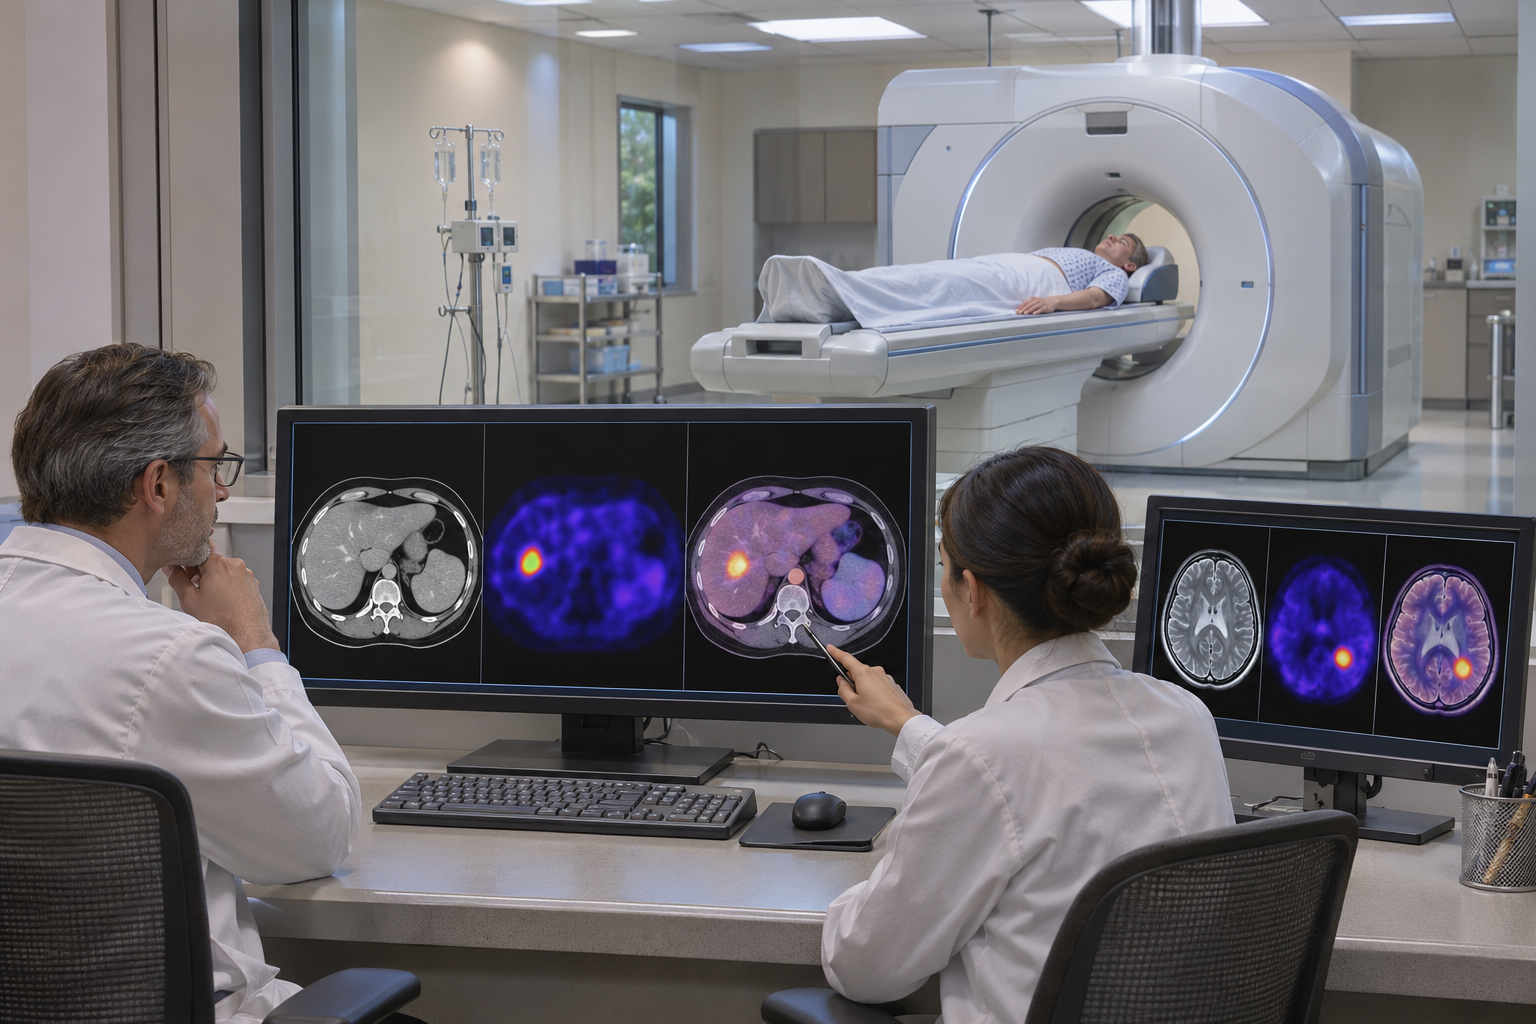
\includegraphics[width=\textwidth,keepaspectratio]{modalities/infographics/hybrid_imaging_realistic.png}
\end{center}
\begin{center}\footnotesize Hybrid imaging registers and combines functional tracer information with anatomical CT or MRI; alignment and the original component images both matter. AI-generated illustration; fused scans are not clinical studies.\end{center}

\section{Overview}
Hybrid imaging combines two or more complementary medical imaging modalities to obtain anatomical, physiological, metabolic, or molecular information within a single examination or a co-registered imaging dataset. Its objective is to address limitations of individual modalities. For example, PET can identify increased metabolic activity but may provide limited anatomical detail, while CT can show the location, dimensions, and morphology of the corresponding lesion.

\begin{center}
\begin{tabular}{@{}p{0.32\textwidth}p{0.22\textwidth}p{0.38\textwidth}@{}}
\toprule
\textbf{Hybrid modality} & \textbf{Anatomical information} & \textbf{Functional or molecular information} \\
\midrule
Fluorescence/X-ray imaging & X-ray & Molecular fluorescence \\
Optical coherence tomography/IVUS & Vascular microstructure & Complementary vascular tissue characterization \\
PET/CT & CT & PET \\
PET/MRI & MRI & PET \\
PET/Ultrasound & Ultrasound & PET \\
Photoacoustic ultrasound & Ultrasound & Optical absorption and tissue oxygenation \\
SPECT/CT & CT & SPECT \\
SPECT/MRI & MRI & SPECT \\
Ultrasound/CT fusion & CT and ultrasound & Real-time ultrasound and Doppler \\
Ultrasound/MRI fusion & MRI and ultrasound & Real-time ultrasound and Doppler \\
\bottomrule
\end{tabular}
\end{center}

PET/CT, PET/MRI, and SPECT/CT are the principal clinically established hybrid imaging modalities. Other combinations are specialized, software-based, or investigational.

The catalogue includes established, supplementary, and investigational applications. Assignments are illustrative rather than formal first-line imaging recommendations. The entries overlap with PET, SPECT, CT, and MRI catalogues and require individual validation against clinical guidance.

\section{Where hybrid imaging is used}
The following examples describe combinations that can add anatomical localization to functional or molecular findings. They do not imply that the listed hybrid examination is always the preferred first-line test.

\subsection{Neurological and neurodegenerative diseases}
\begin{enumerate}[leftmargin=*,itemsep=0.45em,topsep=0.4em]
\item \textbf{Alzheimer disease.} Useful imaging findings include: PET/MRI. Characteristic Imaging Findings: Regional hypometabolism, amyloid deposition and cerebral atrophy.
\item \textbf{Amyotrophic lateral sclerosis.} Useful imaging findings include: PET/MRI. Characteristic Imaging Findings: Reported metabolic and structural motor pathway abnormalities.
\item \textbf{Corticobasal syndrome.} Useful imaging findings include: PET/MRI. Characteristic Imaging Findings: Asymmetric cortical atrophy and hypometabolism.
\item \textbf{Dementia with Lewy bodies.} Useful imaging findings include: PET/MRI. Characteristic Imaging Findings: Occipital hypometabolism with structural assessment.
\item \textbf{Frontotemporal dementia.} Useful imaging findings include: PET/MRI. Characteristic Imaging Findings: Frontal and temporal hypometabolism with corresponding atrophy.
\item \textbf{Huntington disease.} Useful imaging findings include: PET/MRI. Characteristic Imaging Findings: Striatal atrophy and hypometabolism.
\item \textbf{Mild cognitive impairment.} Useful imaging findings include: PET/MRI. Characteristic Imaging Findings: Altered cerebral metabolism or amyloid burden.
\item \textbf{Multiple system atrophy.} Useful imaging findings include: PET/MRI. Characteristic Imaging Findings: Regional hypometabolism and characteristic structural changes.
\item \textbf{Neuroinflammatory disorders.} Useful imaging findings include: PET/MRI. Characteristic Imaging Findings: Molecular tracer abnormalities correlated with structural lesions.
\item \textbf{Parkinson disease.} Useful imaging findings include: SPECT/CT. Characteristic Imaging Findings: Reduced striatal dopamine transporter binding.
\item \textbf{Posterior cortical atrophy.} Useful imaging findings include: PET/MRI. Characteristic Imaging Findings: Posterior cortical hypometabolism and atrophy.
\item \textbf{Primary progressive aphasia.} Useful imaging findings include: PET/MRI. Characteristic Imaging Findings: Regional language network hypometabolism and atrophy.
\item \textbf{Progressive supranuclear palsy.} Useful imaging findings include: PET/MRI. Characteristic Imaging Findings: Midbrain atrophy and regional hypometabolism.
\item \textbf{Vascular dementia.} Useful imaging findings include: PET/MRI. Characteristic Imaging Findings: Regional hypometabolism associated with ischemic lesions.
\end{enumerate}

\subsection{Epilepsy}
\begin{enumerate}[leftmargin=*,itemsep=0.45em,topsep=0.4em]
\item \textbf{Drug-resistant focal epilepsy.} Useful imaging findings include: SPECT/CT, PET/MRI. Characteristic Imaging Findings: Ictal hyperperfusion or interictal hypometabolism.
\item \textbf{Focal cortical dysplasia.} Useful imaging findings include: PET/MRI. Characteristic Imaging Findings: Cortical structural abnormalities and altered metabolism.
\item \textbf{Frontal lobe epilepsy.} Useful imaging findings include: PET/MRI. Characteristic Imaging Findings: Regional frontal hypometabolism.
\item \textbf{Mesial temporal sclerosis.} Useful imaging findings include: PET/MRI. Characteristic Imaging Findings: Hippocampal atrophy, abnormal MRI signal and hypometabolism.
\item \textbf{MRI-negative focal epilepsy.} Useful imaging findings include: PET/MRI. Characteristic Imaging Findings: Regional hypometabolism without obvious structural pathology.
\item \textbf{Occipital lobe epilepsy.} Useful imaging findings include: PET/MRI. Characteristic Imaging Findings: Occipital metabolic abnormalities.
\item \textbf{Parietal lobe epilepsy.} Useful imaging findings include: PET/MRI. Characteristic Imaging Findings: Regional parietal hypometabolism.
\item \textbf{Temporal lobe epilepsy.} Useful imaging findings include: PET/MRI. Characteristic Imaging Findings: Temporal hypometabolism and possible hippocampal sclerosis.
\end{enumerate}

\subsection{Brain tumors}
\begin{enumerate}[leftmargin=*,itemsep=0.45em,topsep=0.4em]
\item \textbf{Astrocytoma.} Useful imaging findings include: PET/MRI. Characteristic Imaging Findings: Variable amino acid uptake and infiltrative MRI abnormalities.
\item \textbf{Brain metastases.} Useful imaging findings include: PET/MRI. Characteristic Imaging Findings: Metabolic abnormalities corresponding to metastatic lesions.
\item \textbf{Ependymoma.} Useful imaging findings include: PET/MRI. Characteristic Imaging Findings: Variable metabolic activity within a structural mass.
\item \textbf{Glioblastoma.} Useful imaging findings include: PET/MRI. Characteristic Imaging Findings: Increased amino acid uptake and infiltrative enhancing mass.
\item \textbf{Medulloblastoma.} Useful imaging findings include: PET/MRI. Characteristic Imaging Findings: Variable metabolic uptake and restricted diffusion.
\item \textbf{Meningioma.} Useful imaging findings include: PET/MRI. Characteristic Imaging Findings: Somatostatin receptor uptake corresponding to a dural mass.
\item \textbf{Oligodendroglioma.} Useful imaging findings include: PET/MRI. Characteristic Imaging Findings: Increased tracer uptake within structurally abnormal tissue.
\item \textbf{Pituitary adenoma.} Useful imaging findings include: PET/MRI. Characteristic Imaging Findings: Focal amino acid tracer uptake within a pituitary lesion.
\item \textbf{Primary CNS lymphoma.} Useful imaging findings include: PET/MRI. Characteristic Imaging Findings: Marked FDG uptake and diffusion restriction.
\item \textbf{Radiation necrosis.} Useful imaging findings include: PET/MRI. Characteristic Imaging Findings: Structural treatment changes with frequently reduced amino acid uptake.
\item \textbf{Recurrent glioma.} Useful imaging findings include: PET/MRI. Characteristic Imaging Findings: Increased amino acid uptake within suspected viable tumor.
\item \textbf{Tumor pseudoprogression.} Useful imaging findings include: PET/MRI. Characteristic Imaging Findings: Variable tracer uptake in treatment-related abnormalities.
\end{enumerate}

\subsection{Cardiovascular diseases}
\begin{enumerate}[leftmargin=*,itemsep=0.45em,topsep=0.4em]
\item \textbf{Cardiac device infection.} Useful imaging findings include: PET/CT. Characteristic Imaging Findings: Abnormal metabolic uptake around implanted devices.
\item \textbf{Cardiac metastases.} Useful imaging findings include: PET/MRI, PET/CT. Characteristic Imaging Findings: Metabolically active myocardial or pericardial lesions.
\item \textbf{Cardiac sarcoidosis.} Useful imaging findings include: PET/MRI, PET/CT. Characteristic Imaging Findings: Focal inflammatory uptake with possible myocardial fibrosis; FDG imaging requires suppression of physiological myocardial uptake.
\item \textbf{Cardiac tumors.} Useful imaging findings include: PET/MRI. Characteristic Imaging Findings: Structural mass with variable metabolic activity.
\item \textbf{Coronary artery disease.} Useful imaging findings include: PET/CT, SPECT/CT. Characteristic Imaging Findings: Myocardial perfusion abnormalities with coronary anatomical information when dedicated CT protocols are used.
\item \textbf{Coronary microvascular dysfunction.} Useful imaging findings include: PET/CT. Characteristic Imaging Findings: Reduced quantitative myocardial flow reserve.
\item \textbf{Dilated cardiomyopathy.} Useful imaging findings include: PET/MRI. Characteristic Imaging Findings: Ventricular dilatation and altered myocardial metabolism.
\item \textbf{Hibernating myocardium.} Useful imaging findings include: PET/MRI, PET/CT. Characteristic Imaging Findings: Reduced perfusion with preserved glucose metabolism.
\item \textbf{Hypertrophic cardiomyopathy.} Useful imaging findings include: PET/MRI. Characteristic Imaging Findings: Myocardial hypertrophy and reduced regional perfusion reserve.
\item \textbf{Ischemic cardiomyopathy.} Useful imaging findings include: PET/MRI. Characteristic Imaging Findings: Perfusion abnormalities and ventricular dysfunction.
\item \textbf{Multivessel coronary artery disease.} Useful imaging findings include: PET/CT. Characteristic Imaging Findings: Reduced absolute myocardial blood flow.
\item \textbf{Myocardial ischemia.} Useful imaging findings include: PET/CT, SPECT/CT. Characteristic Imaging Findings: Reversible myocardial perfusion defects.
\item \textbf{Myocarditis.} Useful imaging findings include: PET/MRI. Characteristic Imaging Findings: Inflammatory uptake and myocardial edema in selected cases.
\item \textbf{Previous myocardial infarction.} Useful imaging findings include: PET/MRI. Characteristic Imaging Findings: Reduced perfusion and myocardial scar.
\item \textbf{Prosthetic valve endocarditis.} Useful imaging findings include: PET/CT, SPECT/CT. Characteristic Imaging Findings: Abnormal inflammatory or leukocyte uptake around prosthetic valves.
\item \textbf{Transthyretin cardiac amyloidosis.} Useful imaging findings include: SPECT/CT. Characteristic Imaging Findings: Myocardial bone-tracer uptake confirmed on SPECT and interpreted with validated criteria.
\end{enumerate}

Bone-tracer uptake alone does not establish ATTR cardiac amyloidosis. Interpretation requires appropriate clinical criteria and evaluation for a monoclonal protein to avoid misclassifying AL amyloidosis.

\subsection{Vascular diseases}
\begin{enumerate}[leftmargin=*,itemsep=0.45em,topsep=0.4em]
\item \textbf{Active vascular microcalcification.} Useful imaging findings include: PET/CT. Characteristic Imaging Findings: Increased ¹⁸F-NaF uptake within vascular plaques.
\item \textbf{Aortitis.} Useful imaging findings include: PET/CT. Characteristic Imaging Findings: Increased aortic wall uptake.
\item \textbf{Atherosclerosis.} Useful imaging findings include: PET/CT. Characteristic Imaging Findings: Plaque-associated inflammatory activity.
\item \textbf{Carotid plaque inflammation.} Useful imaging findings include: PET/MRI. Characteristic Imaging Findings: Plaque morphology and inflammatory metabolic activity.
\item \textbf{Giant cell arteritis.} Useful imaging findings include: PET/CT. Characteristic Imaging Findings: Increased metabolic activity along large arterial walls.
\item \textbf{Infected aortic aneurysm.} Useful imaging findings include: PET/CT. Characteristic Imaging Findings: Aneurysmal morphology with inflammatory uptake.
\item \textbf{Inflammatory abdominal aortic aneurysm.} Useful imaging findings include: PET/CT. Characteristic Imaging Findings: Periaortic inflammatory metabolic activity.
\item \textbf{Moyamoya disease.} Useful imaging findings include: PET/MRI. Characteristic Imaging Findings: Impaired cerebral perfusion associated with vascular abnormalities.
\item \textbf{Takayasu arteritis.} Useful imaging findings include: PET/CT, PET/MRI. Characteristic Imaging Findings: Arterial wall inflammation and structural vascular abnormalities.
\item \textbf{Vascular graft infection.} Useful imaging findings include: PET/CT, SPECT/CT. Characteristic Imaging Findings: Abnormal tracer accumulation around vascular prostheses.
\end{enumerate}
Several vascular molecular imaging applications remain investigational.

\subsection{Pulmonary and thoracic diseases}
\begin{enumerate}[leftmargin=*,itemsep=0.45em,topsep=0.4em]
\item \textbf{Acute pulmonary embolism.} Useful imaging findings include: V/Q SPECT/CT. Characteristic Imaging Findings: Segmental ventilation-perfusion mismatch.
\item \textbf{Bronchial carcinoid.} Useful imaging findings include: PET/CT. Characteristic Imaging Findings: Somatostatin receptor-positive pulmonary lesion.
\item \textbf{Chronic obstructive pulmonary disease.} Useful imaging findings include: SPECT/CT. Characteristic Imaging Findings: Regional ventilation and perfusion abnormalities.
\item \textbf{Chronic thromboembolic pulmonary hypertension.} Useful imaging findings include: V/Q SPECT/CT. Characteristic Imaging Findings: Persistent mismatched perfusion defects.
\item \textbf{Malignant pleural mesothelioma.} Useful imaging findings include: PET/CT. Characteristic Imaging Findings: Pleural thickening with increased metabolic activity.
\item \textbf{Non-small cell lung carcinoma.} Useful imaging findings include: PET/CT. Characteristic Imaging Findings: Hypermetabolic pulmonary mass and possible metastatic lesions.
\item \textbf{Pulmonary adenocarcinoma.} Useful imaging findings include: PET/CT. Characteristic Imaging Findings: Pulmonary lesion with variable FDG uptake.
\item \textbf{Pulmonary fibrosis.} Useful imaging findings include: PET/CT (investigational). Characteristic Imaging Findings: Variable FDG uptake reported in research; PET/CT is not a routine test to diagnose pulmonary fibrosis.
\item \textbf{Pulmonary metastases.} Useful imaging findings include: PET/CT. Characteristic Imaging Findings: Structural pulmonary nodules with variable metabolic uptake.
\item \textbf{Pulmonary sarcoidosis.} Useful imaging findings include: PET/CT. Characteristic Imaging Findings: Metabolically active pulmonary and nodal granulomatous lesions.
\item \textbf{Pulmonary squamous cell carcinoma.} Useful imaging findings include: PET/CT. Characteristic Imaging Findings: Frequently intense uptake within a pulmonary mass.
\item \textbf{Pulmonary tuberculosis.} Useful imaging findings include: PET/CT. Characteristic Imaging Findings: Structural pulmonary abnormalities with inflammatory uptake.
\item \textbf{Small cell lung carcinoma.} Useful imaging findings include: PET/CT. Characteristic Imaging Findings: Metabolically active primary and metastatic disease.
\item \textbf{Solitary pulmonary nodule.} Useful imaging findings include: PET/CT. Characteristic Imaging Findings: Anatomical nodule with variable metabolic activity.
\item \textbf{Thymic carcinoma.} Useful imaging findings include: PET/CT. Characteristic Imaging Findings: Frequently hypermetabolic mediastinal mass.
\item \textbf{Thymoma.} Useful imaging findings include: PET/CT. Characteristic Imaging Findings: Anterior mediastinal mass with variable uptake.
\end{enumerate}

\subsection{Head and neck diseases}
\begin{enumerate}[leftmargin=*,itemsep=0.45em,topsep=0.4em]
\item \textbf{Adenoid cystic carcinoma.} Useful imaging findings include: PET/MRI. Characteristic Imaging Findings: Variable metabolic uptake and possible perineural extension on MRI.
\item \textbf{Cervical lymph node metastases.} Useful imaging findings include: PET/CT. Characteristic Imaging Findings: Hypermetabolic cervical lymph nodes.
\item \textbf{Esthesioneuroblastoma.} Useful imaging findings include: PET/CT, PET/MRI. Characteristic Imaging Findings: Metabolic or receptor-specific uptake within a sinonasal mass.
\item \textbf{Hypopharyngeal carcinoma.} Useful imaging findings include: PET/CT. Characteristic Imaging Findings: Hypermetabolic primary lesion.
\item \textbf{Laryngeal carcinoma.} Useful imaging findings include: PET/CT. Characteristic Imaging Findings: Increased metabolic uptake within a laryngeal mass.
\item \textbf{Nasopharyngeal carcinoma.} Useful imaging findings include: PET/MRI. Characteristic Imaging Findings: Metabolic abnormalities with skull base and soft-tissue assessment.
\item \textbf{Occult head and neck primary tumor.} Useful imaging findings include: PET/CT. Characteristic Imaging Findings: Potential localization of an otherwise unidentified primary malignancy.
\item \textbf{Oral squamous cell carcinoma.} Useful imaging findings include: PET/CT. Characteristic Imaging Findings: Hypermetabolic primary lesion and possible nodal involvement.
\item \textbf{Oropharyngeal carcinoma.} Useful imaging findings include: PET/CT. Characteristic Imaging Findings: Increased primary and nodal metabolic uptake.
\item \textbf{Salivary gland carcinoma.} Useful imaging findings include: PET/MRI. Characteristic Imaging Findings: Variable metabolic activity within a glandular mass.
\item \textbf{Sinonasal carcinoma.} Useful imaging findings include: PET/MRI. Characteristic Imaging Findings: Metabolic activity with detailed anatomical extension.
\item \textbf{Tongue carcinoma.} Useful imaging findings include: PET/MRI. Characteristic Imaging Findings: Metabolic activity with detailed soft-tissue extension.
\end{enumerate}

\subsection{Thyroid and parathyroid diseases}
\begin{enumerate}[leftmargin=*,itemsep=0.45em,topsep=0.4em]
\item \textbf{Anaplastic thyroid carcinoma.} Useful imaging findings include: PET/CT. Characteristic Imaging Findings: Intense metabolic activity within an aggressive mass.
\item \textbf{Ectopic parathyroid adenoma.} Useful imaging findings include: SPECT/CT, PET/CT. Characteristic Imaging Findings: Focal tracer accumulation at an abnormal anatomical location.
\item \textbf{Ectopic thyroid tissue.} Useful imaging findings include: SPECT/CT. Characteristic Imaging Findings: Anatomical localization of functioning thyroid tissue.
\item \textbf{Follicular thyroid carcinoma.} Useful imaging findings include: SPECT/CT. Characteristic Imaging Findings: Radioiodine-avid metastatic lesions.
\item \textbf{Medullary thyroid carcinoma.} Useful imaging findings include: PET/CT. Characteristic Imaging Findings: Amino acid or metabolic tracer uptake.
\item \textbf{Papillary thyroid carcinoma.} Useful imaging findings include: SPECT/CT. Characteristic Imaging Findings: Localization of radioiodine-avid residual or metastatic tissue.
\item \textbf{Parathyroid adenoma.} Useful imaging findings include: SPECT/CT. Characteristic Imaging Findings: Persistent sestamibi uptake localized to a parathyroid lesion.
\item \textbf{Parathyroid hyperplasia.} Useful imaging findings include: SPECT/CT. Characteristic Imaging Findings: Tracer uptake in hyperfunctioning glands.
\item \textbf{Radioiodine-refractory thyroid carcinoma.} Useful imaging findings include: PET/CT. Characteristic Imaging Findings: Hypermetabolic non-iodine-avid tumor lesions.
\item \textbf{Recurrent hyperparathyroidism.} Useful imaging findings include: PET/CT. Characteristic Imaging Findings: Fluorocholine uptake in residual hyperfunctioning tissue.
\end{enumerate}

\subsection{Breast diseases}
\begin{enumerate}[leftmargin=*,itemsep=0.45em,topsep=0.4em]
\item \textbf{Breast cancer sentinel node localization.} Useful imaging findings include: SPECT/CT (selected adjunct). Characteristic Imaging Findings: SPECT/CT can localize nodes when planar lymphoscintigraphy is inadequate or drainage is anatomically complex.
\item \textbf{HER2-positive breast cancer.} Useful imaging findings include: PET/CT. Characteristic Imaging Findings: Variable tumor metabolic activity.
\item \textbf{Inflammatory breast cancer.} Useful imaging findings include: PET/CT. Characteristic Imaging Findings: Diffuse breast and cutaneous metabolic abnormalities.
\item \textbf{Invasive ductal carcinoma.} Useful imaging findings include: PET/CT, PET/MRI. Characteristic Imaging Findings: Increased metabolic uptake and structural breast lesion.
\item \textbf{Invasive lobular carcinoma.} Useful imaging findings include: PET/MRI. Characteristic Imaging Findings: Infiltrative MRI abnormalities with variable metabolic uptake.
\item \textbf{Metastatic breast carcinoma.} Useful imaging findings include: PET/CT. Characteristic Imaging Findings: Metabolically active distant lesions.
\item \textbf{Multifocal breast carcinoma.} Useful imaging findings include: PET/MRI. Characteristic Imaging Findings: Multiple anatomical and metabolically abnormal lesions.
\item \textbf{Recurrent breast carcinoma.} Useful imaging findings include: PET/CT. Characteristic Imaging Findings: Metabolic activity within suspected recurrent disease.
\item \textbf{Recurrent or metastatic breast cancer with uncertain estrogen receptor status.} Useful imaging findings include: FES PET/CT (selected use). Characteristic Imaging Findings: May detect ER-positive lesions as an adjunct to biopsy; not a general breast cancer test.
\item \textbf{Triple-negative breast cancer.} Useful imaging findings include: PET/CT. Characteristic Imaging Findings: Frequently increased glucose metabolism.
\end{enumerate}

\subsection{Hematological malignancies}
\begin{enumerate}[leftmargin=*,itemsep=0.45em,topsep=0.4em]
\item \textbf{Anaplastic large cell lymphoma.} Useful imaging findings include: PET/CT. Characteristic Imaging Findings: Metabolically active nodal and extranodal disease.
\item \textbf{Burkitt lymphoma.} Useful imaging findings include: PET/CT. Characteristic Imaging Findings: Markedly hypermetabolic tumor masses.
\item \textbf{Diffuse large B-cell lymphoma.} Useful imaging findings include: PET/CT. Characteristic Imaging Findings: Intense metabolic uptake within lymphoma lesions.
\item \textbf{Extramedullary plasmacytoma.} Useful imaging findings include: PET/CT. Characteristic Imaging Findings: Hypermetabolic soft-tissue mass.
\item \textbf{Follicular lymphoma.} Useful imaging findings include: PET/CT. Characteristic Imaging Findings: Metabolically active lymphadenopathy.
\item \textbf{Hodgkin lymphoma.} Useful imaging findings include: PET/CT. Characteristic Imaging Findings: Hypermetabolic nodal and extranodal disease.
\item \textbf{Mantle cell lymphoma.} Useful imaging findings include: PET/CT. Characteristic Imaging Findings: Variable metabolic nodal and extranodal involvement.
\item \textbf{Marginal zone lymphoma.} Useful imaging findings include: PET/CT. Characteristic Imaging Findings: Variable metabolic activity.
\item \textbf{Multiple myeloma.} Useful imaging findings include: PET/CT, PET/MRI. Characteristic Imaging Findings: Metabolically active skeletal and marrow lesions.
\item \textbf{Myeloid sarcoma.} Useful imaging findings include: PET/CT. Characteristic Imaging Findings: Metabolically active extramedullary tumor.
\item \textbf{Peripheral T-cell lymphoma.} Useful imaging findings include: PET/CT. Characteristic Imaging Findings: Increased metabolic uptake.
\item \textbf{Primary mediastinal B-cell lymphoma.} Useful imaging findings include: PET/CT. Characteristic Imaging Findings: Hypermetabolic mediastinal mass.
\item \textbf{Richter transformation.} Useful imaging findings include: PET/CT. Characteristic Imaging Findings: Intensely metabolically active suspicious lesions.
\item \textbf{Solitary plasmacytoma.} Useful imaging findings include: PET/CT. Characteristic Imaging Findings: Focal metabolically active plasma cell lesion.
\end{enumerate}

\subsection{Gastrointestinal malignancies}
\begin{enumerate}[leftmargin=*,itemsep=0.45em,topsep=0.4em]
\item \textbf{Anal squamous cell carcinoma.} Useful imaging findings include: PET/CT. Characteristic Imaging Findings: Hypermetabolic primary and nodal lesions.
\item \textbf{Appendiceal carcinoma.} Useful imaging findings include: PET/CT. Characteristic Imaging Findings: Variable metabolic activity.
\item \textbf{Colorectal carcinoma.} Useful imaging findings include: PET/CT. Characteristic Imaging Findings: Hypermetabolic primary or metastatic lesions.
\item \textbf{Esophageal carcinoma.} Useful imaging findings include: PET/CT. Characteristic Imaging Findings: Hypermetabolic esophageal mass and metastatic involvement.
\item \textbf{Gastric carcinoma.} Useful imaging findings include: PET/CT. Characteristic Imaging Findings: Variable metabolic uptake within gastric lesions.
\item \textbf{Gastrointestinal lymphoma.} Useful imaging findings include: PET/CT. Characteristic Imaging Findings: Metabolically active intestinal wall abnormalities.
\item \textbf{Gastrointestinal stromal tumor.} Useful imaging findings include: PET/CT. Characteristic Imaging Findings: Metabolic activity within viable tumor.
\item \textbf{Peritoneal carcinomatosis.} Useful imaging findings include: PET/CT, PET/MRI. Characteristic Imaging Findings: Metabolically active peritoneal deposits.
\item \textbf{Rectal carcinoma.} Useful imaging findings include: PET/MRI. Characteristic Imaging Findings: Tumor metabolism with detailed local anatomical assessment.
\item \textbf{Recurrent colorectal carcinoma.} Useful imaging findings include: PET/CT. Characteristic Imaging Findings: Abnormal metabolic uptake within recurrent lesions.
\item \textbf{Recurrent rectal carcinoma.} Useful imaging findings include: PET/MRI. Characteristic Imaging Findings: Metabolic abnormalities correlated with pelvic soft-tissue changes.
\item \textbf{Small bowel adenocarcinoma.} Useful imaging findings include: PET/CT. Characteristic Imaging Findings: Focal metabolically active intestinal mass.
\end{enumerate}

\subsection{Liver, biliary and pancreatic diseases}
\begin{enumerate}[leftmargin=*,itemsep=0.45em,topsep=0.4em]
\item \textbf{Extrahepatic cholangiocarcinoma.} Useful imaging findings include: PET/CT. Characteristic Imaging Findings: Abnormal biliary tumor uptake.
\item \textbf{Focal nodular hyperplasia.} Useful imaging findings include: SPECT/CT. Characteristic Imaging Findings: Preserved or increased colloid uptake in selected lesions.
\item \textbf{Gallbladder carcinoma.} Useful imaging findings include: PET/CT. Characteristic Imaging Findings: Hypermetabolic gallbladder mass.
\item \textbf{Hepatic hemangioma.} Useful imaging findings include: SPECT/CT. Characteristic Imaging Findings: Delayed blood-pool tracer accumulation.
\item \textbf{Hepatic metastases.} Useful imaging findings include: PET/MRI. Characteristic Imaging Findings: Metabolic abnormalities with high-resolution liver imaging.
\item \textbf{Hepatic neuroendocrine metastases.} Useful imaging findings include: PET/MRI. Characteristic Imaging Findings: Receptor-specific uptake within hepatic lesions.
\item \textbf{Hepatocellular carcinoma.} Useful imaging findings include: PET/MRI. Characteristic Imaging Findings: Characteristic MRI enhancement with variable metabolic uptake.
\item \textbf{Intrahepatic cholangiocarcinoma.} Useful imaging findings include: PET/CT, PET/MRI. Characteristic Imaging Findings: Metabolically active hepatic mass.
\item \textbf{Pancreatic adenocarcinoma.} Useful imaging findings include: PET/CT. Characteristic Imaging Findings: Hypermetabolic pancreatic mass.
\item \textbf{Pancreatic neuroendocrine tumor.} Useful imaging findings include: PET/CT, PET/MRI. Characteristic Imaging Findings: Somatostatin receptor-positive pancreatic lesion.
\item \textbf{Postoperative bile leak.} Useful imaging findings include: SPECT/CT. Characteristic Imaging Findings: Anatomical localization of extraluminal biliary tracer.
\item \textbf{Recurrent pancreatic carcinoma.} Useful imaging findings include: PET/CT. Characteristic Imaging Findings: Metabolic uptake at suspected recurrence sites.
\end{enumerate}

\subsection{Neuroendocrine and adrenal tumors}
\begin{enumerate}[leftmargin=*,itemsep=0.45em,topsep=0.4em]
\item \textbf{Adrenocortical carcinoma.} Useful imaging findings include: PET/CT. Characteristic Imaging Findings: Metabolically active adrenal mass.
\item \textbf{Gastrinoma.} Useful imaging findings include: PET/CT. Characteristic Imaging Findings: Somatostatin receptor-positive tumor.
\item \textbf{Gastroenteropancreatic neuroendocrine tumor.} Useful imaging findings include: PET/CT. Characteristic Imaging Findings: Somatostatin receptor-positive lesions.
\item \textbf{Glucagonoma.} Useful imaging findings include: PET/CT. Characteristic Imaging Findings: Receptor-specific pancreatic tumor uptake.
\item \textbf{Insulinoma.} Useful imaging findings include: PET/CT, PET/MRI. Characteristic Imaging Findings: GLP-1 receptor-specific uptake in selected tumors.
\item \textbf{Merkel cell carcinoma.} Useful imaging findings include: PET/CT. Characteristic Imaging Findings: Hypermetabolic primary or metastatic lesions.
\item \textbf{Neuroblastoma.} Useful imaging findings include: SPECT/CT. Characteristic Imaging Findings: MIBG-avid primary and metastatic lesions.
\item \textbf{Paraganglioma.} Useful imaging findings include: PET/CT. Characteristic Imaging Findings: Frequently intense somatostatin receptor uptake.
\item \textbf{Pheochromocytoma.} Useful imaging findings include: PET/CT, SPECT/CT. Characteristic Imaging Findings: Receptor-specific or MIBG uptake within adrenal lesions.
\item \textbf{Poorly differentiated neuroendocrine carcinoma.} Useful imaging findings include: PET/CT. Characteristic Imaging Findings: Frequently intense FDG uptake.
\item \textbf{Small bowel neuroendocrine tumor.} Useful imaging findings include: PET/CT. Characteristic Imaging Findings: Receptor-positive intestinal and metastatic lesions.
\item \textbf{VIPoma.} Useful imaging findings include: PET/CT. Characteristic Imaging Findings: Increased receptor-specific uptake.
\item \textbf{Well-differentiated neuroendocrine tumor.} Useful imaging findings include: PET/CT. Characteristic Imaging Findings: Increased receptor-specific tracer uptake.
\end{enumerate}

\subsection{Male reproductive and urinary diseases}
\begin{enumerate}[leftmargin=*,itemsep=0.45em,topsep=0.4em]
\item \textbf{Bladder carcinoma.} Useful imaging findings include: PET/CT. Characteristic Imaging Findings: Metabolic uptake in selected primary or metastatic lesions.
\item \textbf{Metastatic castration-resistant prostate cancer.} Useful imaging findings include: PSMA PET/CT. Characteristic Imaging Findings: Variable PSMA expression across metastatic lesions.
\item \textbf{Neuroendocrine prostate carcinoma.} Useful imaging findings include: FDG PET/CT. Characteristic Imaging Findings: Increased glucose metabolism with potentially reduced PSMA uptake.
\item \textbf{Penile carcinoma.} Useful imaging findings include: PET/CT. Characteristic Imaging Findings: Metabolically active primary or nodal lesions.
\item \textbf{Prostate adenocarcinoma.} Useful imaging findings include: PSMA PET/CT, PET/MRI. Characteristic Imaging Findings: Increased PSMA uptake within primary or metastatic lesions.
\item \textbf{Prostate lesion requiring targeted biopsy.} Useful imaging findings include: MRI/Ultrasound fusion. Characteristic Imaging Findings: MRI-defined suspicious lesion localized using real-time ultrasound.
\item \textbf{Recurrent prostate carcinoma.} Useful imaging findings include: PSMA PET/CT. Characteristic Imaging Findings: Localization of recurrent or metastatic disease.
\item \textbf{Renal cell carcinoma.} Useful imaging findings include: PET/CT. Characteristic Imaging Findings: Variable metabolic activity within metastatic lesions.
\item \textbf{Renal lymphoma.} Useful imaging findings include: PET/CT. Characteristic Imaging Findings: Hypermetabolic renal lesions.
\item \textbf{Testicular seminoma.} Useful imaging findings include: PET/CT. Characteristic Imaging Findings: Metabolic activity within selected residual masses.
\end{enumerate}

\subsection{Female reproductive diseases}
\begin{enumerate}[leftmargin=*,itemsep=0.45em,topsep=0.4em]
\item \textbf{Cervical carcinoma.} Useful imaging findings include: PET/MRI. Characteristic Imaging Findings: Metabolic activity with detailed parametrial and pelvic anatomy.
\item \textbf{Endometrial carcinoma.} Useful imaging findings include: PET/MRI. Characteristic Imaging Findings: Metabolic tumor activity and myometrial invasion assessment.
\item \textbf{Endometrial stromal sarcoma.} Useful imaging findings include: PET/MRI. Characteristic Imaging Findings: Variable metabolic activity within a uterine lesion.
\item \textbf{Fallopian tube carcinoma.} Useful imaging findings include: PET/CT. Characteristic Imaging Findings: Metabolically active adnexal or metastatic lesions.
\item \textbf{Ovarian carcinoma.} Useful imaging findings include: PET/CT, PET/MRI. Characteristic Imaging Findings: Metabolically active pelvic and peritoneal lesions.
\item \textbf{Primary peritoneal carcinoma.} Useful imaging findings include: PET/CT. Characteristic Imaging Findings: Hypermetabolic peritoneal deposits.
\item \textbf{Recurrent ovarian carcinoma.} Useful imaging findings include: PET/CT. Characteristic Imaging Findings: Metabolic uptake within recurrent lesions.
\item \textbf{Uterine leiomyosarcoma.} Useful imaging findings include: PET/MRI. Characteristic Imaging Findings: Metabolic activity within a heterogeneous uterine mass.
\item \textbf{Vaginal carcinoma.} Useful imaging findings include: PET/MRI. Characteristic Imaging Findings: Metabolic uptake with local soft-tissue characterization.
\item \textbf{Vulvar carcinoma.} Useful imaging findings include: PET/CT. Characteristic Imaging Findings: Metabolically active primary and nodal lesions.
\end{enumerate}

\subsection{Bone and skeletal diseases}
\begin{enumerate}[leftmargin=*,itemsep=0.45em,topsep=0.4em]
\item \textbf{Bone lymphoma.} Useful imaging findings include: PET/CT. Characteristic Imaging Findings: Hypermetabolic bone or marrow lesions.
\item \textbf{Chondrosarcoma.} Useful imaging findings include: PET/CT. Characteristic Imaging Findings: Variable tumor metabolism.
\item \textbf{Ewing sarcoma.} Useful imaging findings include: PET/CT. Characteristic Imaging Findings: Increased metabolic activity within a skeletal mass.
\item \textbf{Fibrous dysplasia.} Useful imaging findings include: SPECT/CT. Characteristic Imaging Findings: Increased skeletal uptake with ground-glass bone morphology.
\item \textbf{Fracture nonunion.} Useful imaging findings include: SPECT/CT. Characteristic Imaging Findings: Abnormal uptake reflecting biological activity at the fracture site.
\item \textbf{Giant cell tumor of bone.} Useful imaging findings include: PET/CT. Characteristic Imaging Findings: Frequently intense metabolic uptake.
\item \textbf{Heterotopic ossification.} Useful imaging findings include: SPECT/CT. Characteristic Imaging Findings: Increased uptake within extraosseous mineralization.
\item \textbf{Occult fracture.} Useful imaging findings include: SPECT/CT. Characteristic Imaging Findings: Increased uptake localized to an otherwise subtle fracture.
\item \textbf{Osteoblastic bone metastases.} Useful imaging findings include: SPECT/CT, PET/CT. Characteristic Imaging Findings: Increased bone turnover localized to skeletal lesions.
\item \textbf{Osteoblastoma.} Useful imaging findings include: SPECT/CT. Characteristic Imaging Findings: Increased uptake within an expansile bone lesion.
\item \textbf{Osteochondral lesion.} Useful imaging findings include: SPECT/CT. Characteristic Imaging Findings: Focal subchondral tracer accumulation.
\item \textbf{Osteoid osteoma.} Useful imaging findings include: SPECT/CT. Characteristic Imaging Findings: Intense focal uptake corresponding to the nidus.
\item \textbf{Osteolytic bone metastases.} Useful imaging findings include: PET/CT. Characteristic Imaging Findings: Metabolic activity within lytic skeletal lesions.
\item \textbf{Osteonecrosis.} Useful imaging findings include: SPECT/CT. Characteristic Imaging Findings: Variable uptake associated with necrosis and repair.
\item \textbf{Osteosarcoma.} Useful imaging findings include: PET/CT. Characteristic Imaging Findings: Hypermetabolic bone tumor.
\item \textbf{Paget disease.} Useful imaging findings include: SPECT/CT. Characteristic Imaging Findings: Increased skeletal remodeling with characteristic bone morphology.
\item \textbf{Sacral insufficiency fracture.} Useful imaging findings include: SPECT/CT. Characteristic Imaging Findings: Characteristic sacral uptake distribution.
\item \textbf{Stress fracture.} Useful imaging findings include: SPECT/CT. Characteristic Imaging Findings: Focal uptake corresponding to a stress injury.
\end{enumerate}

\subsection{Joint and spinal diseases}
\begin{enumerate}[leftmargin=*,itemsep=0.45em,topsep=0.4em]
\item \textbf{Aseptic prosthetic loosening.} Useful imaging findings include: SPECT/CT. Characteristic Imaging Findings: Increased uptake at prosthetic interfaces.
\item \textbf{Cervical facet arthropathy.} Useful imaging findings include: SPECT/CT. Characteristic Imaging Findings: Focal facet joint tracer accumulation.
\item \textbf{Charcot arthropathy.} Useful imaging findings include: SPECT/CT. Characteristic Imaging Findings: Marked skeletal remodeling and joint destruction.
\item \textbf{Degenerative disc disease.} Useful imaging findings include: SPECT/CT. Characteristic Imaging Findings: Increased vertebral endplate bone turnover.
\item \textbf{Lumbar facet arthropathy.} Useful imaging findings include: SPECT/CT. Characteristic Imaging Findings: Increased uptake localized to facet joints.
\item \textbf{Osteoarthritis.} Useful imaging findings include: SPECT/CT. Characteristic Imaging Findings: Increased subchondral bone remodeling.
\item \textbf{Painful hip arthroplasty.} Useful imaging findings include: SPECT/CT. Characteristic Imaging Findings: Abnormal uptake around acetabular or femoral components.
\item \textbf{Painful knee arthroplasty.} Useful imaging findings include: SPECT/CT. Characteristic Imaging Findings: Abnormal compartmental or periprosthetic uptake.
\item \textbf{Prosthetic joint infection.} Useful imaging findings include: Leukocyte SPECT/CT. Characteristic Imaging Findings: Abnormal leukocyte localization around prosthetic components.
\item \textbf{Rheumatoid arthritis.} Useful imaging findings include: PET/CT. Characteristic Imaging Findings: Increased inflammatory synovial activity.
\item \textbf{Sacroiliitis.} Useful imaging findings include: PET/MRI. Characteristic Imaging Findings: Structural inflammatory abnormalities with variable tracer uptake.
\item \textbf{Septic arthritis.} Useful imaging findings include: PET/CT, SPECT/CT. Characteristic Imaging Findings: Abnormal inflammatory tracer accumulation.
\item \textbf{Spinal fusion pseudarthrosis.} Useful imaging findings include: SPECT/CT. Characteristic Imaging Findings: Persistent uptake at the fusion site.
\item \textbf{Spinal hardware loosening.} Useful imaging findings include: SPECT/CT. Characteristic Imaging Findings: Abnormal peri-implant uptake.
\item \textbf{Spondylolysis.} Useful imaging findings include: SPECT/CT. Characteristic Imaging Findings: Increased uptake within an active pars defect.
\end{enumerate}

\subsection{Soft-tissue and skin malignancies}
\begin{enumerate}[leftmargin=*,itemsep=0.45em,topsep=0.4em]
\item \textbf{Angiosarcoma.} Useful imaging findings include: PET/CT. Characteristic Imaging Findings: Variable increased tumor metabolism.
\item \textbf{Cutaneous lymphoma.} Useful imaging findings include: PET/CT. Characteristic Imaging Findings: Variable metabolically active cutaneous lesions.
\item \textbf{Cutaneous squamous cell carcinoma.} Useful imaging findings include: PET/CT. Characteristic Imaging Findings: Increased uptake in advanced primary or metastatic disease.
\item \textbf{Leiomyosarcoma.} Useful imaging findings include: PET/CT. Characteristic Imaging Findings: Increased metabolism within viable tumor.
\item \textbf{Liposarcoma.} Useful imaging findings include: PET/MRI. Characteristic Imaging Findings: Structural fatty or soft-tissue mass with variable metabolism.
\item \textbf{Malignant melanoma.} Useful imaging findings include: PET/CT. Characteristic Imaging Findings: Metabolically active metastatic lesions.
\item \textbf{Malignant peripheral nerve sheath tumor.} Useful imaging findings include: PET/MRI. Characteristic Imaging Findings: Increased uptake within a nerve-associated mass.
\item \textbf{Rhabdomyosarcoma.} Useful imaging findings include: PET/MRI. Characteristic Imaging Findings: Metabolic tumor activity with detailed tissue extension.
\item \textbf{Synovial sarcoma.} Useful imaging findings include: PET/MRI. Characteristic Imaging Findings: Metabolic activity within a soft-tissue mass.
\item \textbf{Undifferentiated pleomorphic sarcoma.} Useful imaging findings include: PET/CT. Characteristic Imaging Findings: Hypermetabolic soft-tissue lesion.
\end{enumerate}

\subsection{Infectious diseases}
\begin{enumerate}[leftmargin=*,itemsep=0.45em,topsep=0.4em]
\item \textbf{Acute osteomyelitis.} Useful imaging findings include: PET/CT, SPECT/CT. Characteristic Imaging Findings: Abnormal osseous inflammatory tracer accumulation.
\item \textbf{Chronic osteomyelitis.} Useful imaging findings include: PET/CT. Characteristic Imaging Findings: Persistent metabolic activity within affected bone.
\item \textbf{Diabetic foot osteomyelitis.} Useful imaging findings include: Leukocyte SPECT/CT. Characteristic Imaging Findings: Localization of leukocyte uptake within infected bone.
\item \textbf{Diabetic foot soft-tissue infection.} Useful imaging findings include: Leukocyte SPECT/CT. Characteristic Imaging Findings: Leukocyte uptake localized to soft tissue.
\item \textbf{Disseminated fungal infection.} Useful imaging findings include: PET/CT. Characteristic Imaging Findings: Multifocal inflammatory uptake.
\item \textbf{Fever of unknown origin.} Useful imaging findings include: PET/CT. Characteristic Imaging Findings: Localization of occult inflammatory or infectious foci.
\item \textbf{Hepatic abscess.} Useful imaging findings include: PET/CT. Characteristic Imaging Findings: Inflammatory uptake surrounding a hepatic collection.
\item \textbf{Infected hepatic cyst.} Useful imaging findings include: PET/CT. Characteristic Imaging Findings: Abnormal cyst-associated inflammatory uptake.
\item \textbf{Infected orthopedic hardware.} Useful imaging findings include: SPECT/CT, PET/CT. Characteristic Imaging Findings: Abnormal peri-implant tracer accumulation.
\item \textbf{Infected renal cyst.} Useful imaging findings include: PET/CT. Characteristic Imaging Findings: Increased metabolic activity within the cyst wall.
\item \textbf{Intra-abdominal abscess.} Useful imaging findings include: PET/CT. Characteristic Imaging Findings: Focal inflammatory activity corresponding to a collection.
\item \textbf{Septic emboli.} Useful imaging findings include: PET/CT. Characteristic Imaging Findings: Multifocal metabolic abnormalities.
\item \textbf{Spondylodiscitis.} Useful imaging findings include: PET/CT. Characteristic Imaging Findings: Metabolic activity involving adjacent vertebrae and disc.
\item \textbf{Tuberculosis.} Useful imaging findings include: PET/CT. Characteristic Imaging Findings: Metabolically active infectious lesions.
\item \textbf{Vertebral osteomyelitis.} Useful imaging findings include: PET/CT. Characteristic Imaging Findings: Increased vertebral inflammatory uptake.
\end{enumerate}

\subsection{Autoimmune and inflammatory diseases}
\begin{enumerate}[leftmargin=*,itemsep=0.45em,topsep=0.4em]
\item \textbf{Autoimmune pancreatitis.} Useful imaging findings include: PET/CT. Characteristic Imaging Findings: Diffuse or focal pancreatic uptake.
\item \textbf{Crohn disease.} Useful imaging findings include: PET/MRI. Characteristic Imaging Findings: Bowel wall inflammation and structural abnormalities.
\item \textbf{Dermatomyositis.} Useful imaging findings include: PET/MRI. Characteristic Imaging Findings: Muscle inflammation and structural MRI abnormalities.
\item \textbf{IgG4-related disease.} Useful imaging findings include: PET/CT. Characteristic Imaging Findings: Multiorgan inflammatory metabolic uptake.
\item \textbf{Polymyalgia rheumatica.} Useful imaging findings include: PET/CT. Characteristic Imaging Findings: Characteristic periarticular and bursal inflammatory uptake.
\item \textbf{Polymyositis.} Useful imaging findings include: PET/MRI. Characteristic Imaging Findings: Increased muscle metabolic activity and edema.
\item \textbf{Psoriatic arthritis.} Useful imaging findings include: PET/MRI. Characteristic Imaging Findings: Joint inflammation and entheseal abnormalities.
\item \textbf{Relapsing polychondritis.} Useful imaging findings include: PET/CT. Characteristic Imaging Findings: Increased uptake within inflamed cartilaginous structures.
\item \textbf{Retroperitoneal fibrosis.} Useful imaging findings include: PET/CT. Characteristic Imaging Findings: Active inflammatory uptake within fibrotic tissue.
\item \textbf{Systemic sarcoidosis.} Useful imaging findings include: PET/CT. Characteristic Imaging Findings: Multiorgan metabolically active granulomatous lesions.
\item \textbf{Ulcerative colitis.} Useful imaging findings include: PET/MRI. Characteristic Imaging Findings: Colonic inflammatory metabolic activity.
\end{enumerate}

\subsection{Renal, lymphatic and splenic disorders}
\begin{enumerate}[leftmargin=*,itemsep=0.45em,topsep=0.4em]
\item \textbf{Accessory spleen.} Useful imaging findings include: SPECT/CT. Characteristic Imaging Findings: Anatomically localized functioning splenic tissue.
\item \textbf{Chylous leakage.} Useful imaging findings include: SPECT/CT. Characteristic Imaging Findings: Anatomical localization of abnormal lymphatic tracer accumulation.
\item \textbf{Ectopic kidney.} Useful imaging findings include: SPECT/CT. Characteristic Imaging Findings: Functioning renal tissue at an abnormal anatomical location.
\item \textbf{Lymphatic obstruction.} Useful imaging findings include: SPECT/CT. Characteristic Imaging Findings: Interrupted lymphatic tracer progression.
\item \textbf{Primary lymphedema.} Useful imaging findings include: SPECT/CT. Characteristic Imaging Findings: Impaired lymphatic drainage.
\item \textbf{Renal cortical scarring.} Useful imaging findings include: SPECT/CT. Characteristic Imaging Findings: Persistent localized cortical uptake defects.
\item \textbf{Renal dysplasia.} Useful imaging findings include: SPECT/CT. Characteristic Imaging Findings: Abnormal renal cortical tracer distribution.
\item \textbf{Renal infarction.} Useful imaging findings include: SPECT/CT. Characteristic Imaging Findings: Regional absence of renal cortical tracer uptake.
\item \textbf{Secondary lymphedema.} Useful imaging findings include: SPECT/CT. Characteristic Imaging Findings: Abnormal lymphatic transport and dermal backflow.
\item \textbf{Splenosis.} Useful imaging findings include: SPECT/CT. Characteristic Imaging Findings: Selective tracer accumulation within ectopic splenic tissue.
\end{enumerate}

\subsection{Summary of catalogue}
\begin{center}
\begin{tabular}{@{}p{0.70\textwidth}r@{}}
\toprule
\textbf{Disease category} & \textbf{Entries} \\
\midrule
Autoimmune and inflammatory diseases & 11 \\
Bone and skeletal diseases & 18 \\
Brain tumors & 12 \\
Breast diseases & 10 \\
Cardiovascular diseases & 16 \\
Epilepsy & 8 \\
Female reproductive diseases & 10 \\
Gastrointestinal malignancies & 12 \\
Head and neck diseases & 12 \\
Hematological malignancies & 14 \\
Infectious diseases & 15 \\
Joint and spinal diseases & 15 \\
Liver, biliary and pancreatic diseases & 12 \\
Male reproductive and urinary diseases & 10 \\
Neuroendocrine and adrenal tumors & 13 \\
Neurological and neurodegenerative diseases & 14 \\
Pulmonary and thoracic diseases & 16 \\
Renal, lymphatic and splenic disorders & 10 \\
Soft-tissue and skin malignancies & 10 \\
Thyroid and parathyroid diseases & 10 \\
Vascular diseases & 10 \\
\midrule
\textbf{Total} & \textbf{258} \\
\bottomrule
\end{tabular}
\end{center}

\subsection{Comparison of major hybrid imaging modalities}
\begin{longtable}{@{}p{0.28\textwidth}p{0.22\textwidth}p{0.22\textwidth}p{0.22\textwidth}@{}}
\toprule
\textbf{Feature} & \textbf{PET/CT} & \textbf{PET/MRI} & \textbf{SPECT/CT} \\
\midrule
\endfirsthead
\toprule
\textbf{Feature} & \textbf{PET/CT} & \textbf{PET/MRI} & \textbf{SPECT/CT} \\
\midrule
\endhead
Acquisition time & Generally shorter & Generally longer & Protocol-dependent \\
Anatomical modality & CT & MRI & CT \\
Attenuation correction & CT-based & MRI-derived or model-based & CT-based \\
Bone morphology & Excellent & Good & Excellent \\
Cardiology & Excellent & Specialized & Widely established \\
Clinical availability & Relatively widespread & Limited & Relatively widespread \\
Equipment cost & High & Very high & Generally lower \\
Ionizing radiation & PET + CT & PET & SPECT + CT \\
Molecular modality & PET & PET & SPECT \\
Molecular sensitivity & High & High & Generally lower \\
Musculoskeletal imaging & Excellent & Excellent for selected indications & Excellent for selected indications \\
Neurology & Excellent & Excellent & Selected applications \\
Oncology & Excellent & Excellent for selected indications & Selected applications \\
Pulmonary anatomy & Excellent & Generally inferior to CT & Excellent with diagnostic CT \\
Soft-tissue contrast & Moderate to high & Excellent & Moderate to high \\
\bottomrule
\end{longtable}

\subsection{Computational principles of hybrid imaging}
Hybrid imaging is fundamentally a multimodal image registration and data fusion problem. Given two volumetric images, $I_A(x,y,z)$ and $I_B(x,y,z)$, the objective is to determine a spatial transformation $T$ that aligns corresponding anatomical structures:
\begin{equation}
T^*=\underset{T}{\arg\max}\;\operatorname{Similarity}(I_A,I_B\circ T).
\end{equation}
For multimodal image registration, mutual information is frequently used:
\begin{equation}
MI(A,B)=H(A)+H(B)-H(A,B),
\end{equation}
where $H(A)$ and $H(B)$ are the marginal entropies and $H(A,B)$ is the joint entropy.

\subsection{Image registration and fusion techniques}
\begin{longtable}{@{}p{0.38\textwidth}p{0.54\textwidth}@{}}
\toprule
\textbf{Technique} & \textbf{Primary application} \\
\midrule
\endfirsthead
\toprule
\textbf{Technique} & \textbf{Primary application} \\
\midrule
\endhead
Affine registration & Scaling, shearing and global alignment \\
B-spline registration & Smooth nonrigid transformations \\
Cardiac motion correction & Myocardial image alignment \\
Decision-level fusion & Integration of modality-specific diagnostic predictions \\
Deep learning registration & Learned spatial transformations \\
Deformable registration & Compensation for local anatomical deformation \\
Diffeomorphic registration & Smooth, invertible anatomical transformations \\
Feature-based registration & Alignment using extracted anatomical features \\
Feature-level fusion & Integration of modality-specific feature representations \\
Landmark-based registration & Alignment using corresponding anatomical landmarks \\
Mutual information registration & Alignment of different imaging modalities \\
Respiratory motion correction & Thoracic and abdominal alignment \\
Rigid registration & Translation and rotation alignment \\
Voxel-level fusion & Integration of registered image intensities \\
\bottomrule
\end{longtable}

\subsection{Quantitative parameters in hybrid imaging}
\begin{longtable}{@{}p{0.34\textwidth}p{0.20\textwidth}p{0.38\textwidth}@{}}
\toprule
\textbf{Parameter} & \textbf{Source modality} & \textbf{Clinical significance} \\
\midrule
\endfirsthead
\toprule
\textbf{Parameter} & \textbf{Source modality} & \textbf{Clinical significance} \\
\midrule
\endhead
Apparent diffusion coefficient & MRI & Tissue diffusivity \\
Dice similarity coefficient & Segmentation & Spatial overlap between segmentation masks \\
Extracellular volume fraction & MRI & Myocardial extracellular expansion \\
Fractional anisotropy & MRI & Directional diffusion properties \\
Hounsfield unit & CT & Tissue attenuation \\
Lesion volume & CT/MRI & Anatomical tumor burden \\
Metabolic tumor volume & PET & Metabolically active tumor burden \\
Myocardial blood flow & PET & Absolute myocardial perfusion \\
Myocardial flow reserve & PET & Coronary functional assessment \\
Specific binding ratio & SPECT & Receptor or transporter availability \\
SULpeak & PET & Metabolic treatment response assessment \\
SUVmax & PET & Maximum normalized tracer uptake \\
SUVmean & PET & Average normalized tracer uptake \\
T1 relaxation time & MRI & Tissue characterization \\
T2 relaxation time & MRI & Tissue water and relaxation characteristics \\
Target registration error & Registration & Spatial alignment accuracy \\
Total lesion glycolysis & PET & Combined glucose-related tracer uptake and volume \\
Tumor-to-background ratio & PET/SPECT & Relative molecular activity \\
\bottomrule
\end{longtable}

\subsection{Established versus emerging hybrid imaging applications}
\begin{longtable}{@{}p{0.58\textwidth}p{0.36\textwidth}@{}}
\toprule
\textbf{Application} & \textbf{Clinical status} \\
\midrule
\endfirsthead
\toprule
\textbf{Application} & \textbf{Clinical status} \\
\midrule
\endhead
AI-based multimodal diagnostic fusion & Emerging \\
FDG PET/CT for lung cancer staging & Established \\
FDG PET/CT for lymphoma staging & Established \\
Leukocyte SPECT/CT for infection localization & Established in selected cases \\
MRI/Ultrasound fusion for prostate biopsy & Established \\
PET/MRI for brain tumor assessment & Specialized clinical application \\
PET/MRI for cardiac inflammation & Emerging and specialized \\
PET/MRI for epilepsy assessment & Specialized clinical application \\
PET/MRI for pediatric oncology & Specialized clinical application \\
PET/MRI for pelvic oncology & Specialized clinical application \\
PET/Ultrasound & Predominantly investigational \\
Photoacoustic ultrasound & Emerging and application-dependent \\
PSMA PET/CT for prostate cancer & Established \\
Somatostatin receptor PET/CT for neuroendocrine tumors & Established \\
SPECT/CT for cardiac amyloidosis & Established in selected patients using validated criteria after evaluation for monoclonal protein \\
SPECT/CT for parathyroid localization & Established \\
SPECT/CT for skeletal lesion characterization & Established \\
SPECT/MRI & Predominantly investigational \\
V/Q SPECT/CT for pulmonary embolism & Established \\
\bottomrule
\end{longtable}

\subsection{Published hybrid medical imaging datasets and resources}
\begin{longtable}{@{}p{0.40\textwidth}p{0.52\textwidth}@{}}
\toprule
\textbf{Source} & \textbf{Primary utility} \\
\midrule
\endfirsthead
\toprule
\textbf{Source} & \textbf{Primary utility} \\
\midrule
\endhead
3D Slicer & Multimodal visualization, registration and segmentation \\
ADNI & Paired MRI and PET neuroimaging \\
ANTs & Advanced medical image registration \\
AutoPET Challenge & Whole-body PET/CT lesion segmentation \\
European Association of Nuclear Medicine & Imaging protocols and clinical standards \\
MONAI & Deep learning for multimodal medical imaging \\
OpenNeuro & Multimodal neurological imaging \\
PubMed Central & Published clinical hybrid imaging studies \\
Radiopaedia & Annotated hybrid imaging clinical cases \\
SimpleITK & Medical image processing and registration \\
Society of Nuclear Medicine and Molecular Imaging & Clinical guidelines \\
The Cancer Imaging Archive & Multimodal oncological imaging datasets \\
\bottomrule
\end{longtable}

\subsection{Recommended metadata for a hybrid imaging dataset}
\begin{longtable}{@{}p{0.45\textwidth}p{0.49\textwidth}@{}}
\toprule
\textbf{Attribute} & \textbf{Example} \\
\midrule
Acquisition relationship & Simultaneous \\
ADC & $0.65 \times 10^{-3}$ mm$^2$/s \\
Administered activity & 150 MBq \\
Anatomical image & MRI volume \\
Anatomical lesion volume & 2.8 cm$^3$ \\
Anatomical modality & Multiparametric MRI \\
Annotation & Three-dimensional lesion segmentation \\
Diagnostic reference standard & Histopathological confirmation \\
Disease & Prostate adenocarcinoma \\
Fused image & Co-registered PET/MRI \\
Hybrid modality & PET/MRI \\
Image format & DICOM or NIfTI \\
Image license & CC BY or other specified license \\
Molecular image & PET volume \\
Molecular modality & PET \\
Molecular target & PSMA \\
MRI component reporting classification & PI-RADS 5 \\
MRI field strength & 3 Tesla \\
MRI sequences & T2, DWI, ADC, DCE \\
Publication reference & DOI or PMID \\
Radiopharmaceutical & ⁶⁸Ga-PSMA-11 \\
Registration error & 1.8 mm \\
Registration technique & Rigid and deformable registration \\
Registration transformation & Stored transformation matrix or deformation field \\
SUVmax & 14.2 \\
Uptake period & 60 minutes \\
\bottomrule
\end{longtable}

\subsection{Hybrid imaging for AI-based medical diagnosis}
From a computational perspective, multimodal diagnostic systems use several common fusion architectures:
\begin{longtable}{@{}p{0.34\textwidth}p{0.60\textwidth}@{}}
\toprule
\textbf{Architecture} & \textbf{Computational approach} \\
\midrule
\endfirsthead
\toprule
\textbf{Architecture} & \textbf{Computational approach} \\
\midrule
\endhead
Cross-modal attention & Learn relationships between different modality representations \\
Early fusion & Combine registered input images before feature extraction \\
Intermediate fusion & Combine modality-specific learned feature representations \\
Late fusion & Combine independently generated diagnostic probabilities \\
\bottomrule
\end{longtable}
A multimodal diagnostic model may be represented as:
\begin{equation}
\hat{y}=f_{\theta}\left(I_{\mathrm{CT}},I_{\mathrm{PET}},I_{\mathrm{MRI}},M_{\mathrm{clinical}}\right),
\end{equation}
where $M_{\mathrm{clinical}}$ represents relevant clinical and acquisition metadata.

\subsection{Complementary diagnostic information}
\begin{longtable}{@{}p{0.42\textwidth}p{0.52\textwidth}@{}}
\toprule
\textbf{Pathological characteristic} & \textbf{Appropriate imaging technique} \\
\midrule
\endfirsthead
\toprule
\textbf{Pathological characteristic} & \textbf{Appropriate imaging technique} \\
\midrule
\endhead
Anatomical morphology & CT, MRI \\
Bone remodeling & SPECT, NaF PET \\
Calcification & CT \\
Cellular microstructure & Diffusion MRI \\
Hemodynamic activity & fMRI \\
Receptor expression & Targeted PET \\
Soft-tissue characterization & MRI \\
Tissue attenuation & CT \\
Tissue perfusion & PET, SPECT, MRI \\
Tissue stiffness & Elastography \\
Tumor glucose metabolism & FDG PET \\
Vascular flow & Doppler ultrasound \\
\bottomrule
\end{longtable}

For a comprehensive medical imaging dataset, hybrid imaging should be classified as a composite modality rather than an independent physical imaging mechanism. Preserve the original component images alongside the fused representation so that quantitative information is not lost.

The catalogue includes established, supplementary, and investigational applications. The modality assignments are illustrative and not formal first-line imaging recommendations. Individual entries require guideline validation, and substantial overlap exists with the PET, SPECT, CT, and MRI catalogues.

\chapter{Interventional Radiology and Cardiac Catheterization}
\label{ch:interventional_radiology_cardiac_catheterization}

% Chapter-opening illustrated modality infographic.
\begin{center}
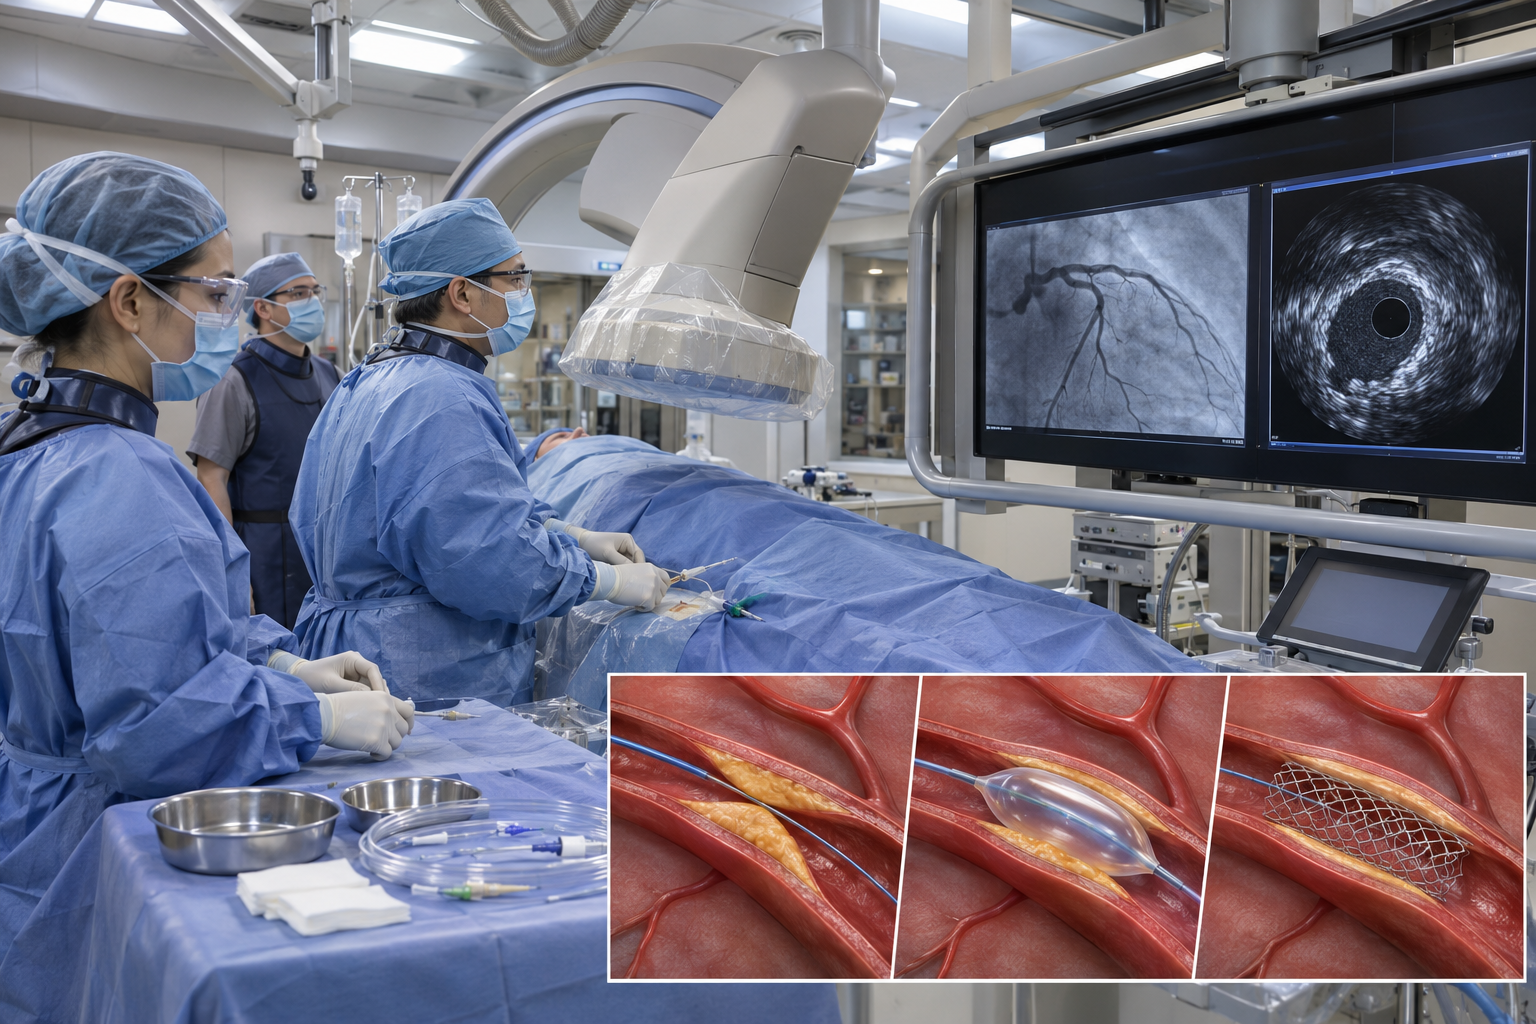
\includegraphics[width=\textwidth,keepaspectratio]{modalities/infographics/interventional_radiology_cardiac_cath_realistic.png}
\end{center}
\begin{center}\footnotesize Image-guided procedures use live imaging to navigate devices and assess treatment; the inset schematically shows catheter-based coronary intervention. AI-generated illustration; no actual procedure is depicted.\end{center}

\section{Overview}
Interventional radiology (IR) and cardiac catheterization are minimally invasive medical disciplines that use image guidance to perform diagnostic and therapeutic procedures. Unlike conventional diagnostic imaging, these disciplines enable physicians to interact directly with anatomical structures using catheters, guidewires, needles, balloons, stents, and other medical devices.

Imaging modalities employed include fluoroscopy, digital subtraction angiography (DSA), computed tomography (CT), ultrasound and Doppler ultrasound, cone-beam CT (CBCT), magnetic resonance imaging (MRI), intravascular ultrasound (IVUS), optical coherence tomography (OCT), and intracardiac echocardiography (ICE).

The catalogue includes diseases, characteristic imaging findings, and associated interventional procedures. It spans diagnostic findings, therapeutic indications, and specialized procedures. Some entries overlap; interventions may be appropriate only for selected patients or remain emerging applications. Individual indications require validation against current clinical guidelines.

\section{Where image-guided intervention is used}
The numbered entries below describe example imaging findings and related procedures. They are not treatment recommendations; decisions depend on the patient's condition, anatomy, risks, and current professional guidance.

\subsection{Part I: Interventional radiology}

\subsubsection{Peripheral arterial diseases}
\begin{enumerate}[leftmargin=*,itemsep=0.45em,topsep=0.4em]
\item \textbf{Acute limb ischemia.} Useful imaging findings include: Abrupt arterial contrast cutoff. Interventional Procedure: Thrombectomy, catheter-directed thrombolysis.
\item \textbf{Aortoiliac occlusive disease.} Useful imaging findings include: Aortoiliac stenosis or occlusion. Interventional Procedure: Angioplasty, stenting.
\item \textbf{Arterial dissection.} Useful imaging findings include: Intimal flap or false lumen. Interventional Procedure: Selected stent placement.
\item \textbf{Arterial embolism.} Useful imaging findings include: Abrupt intraluminal filling defect. Interventional Procedure: Catheter thrombectomy.
\item \textbf{Arterial thrombosis.} Useful imaging findings include: Intraluminal filling defect or complete occlusion. Interventional Procedure: Thrombectomy, thrombolysis.
\item \textbf{Buerger disease.} Useful imaging findings include: Distal arterial occlusions and corkscrew collaterals. Interventional Procedure: Selected endovascular revascularization.
\item \textbf{Chronic limb-threatening ischemia.} Useful imaging findings include: Multilevel occlusive disease and poor distal runoff. Interventional Procedure: Endovascular revascularization.
\item \textbf{Femoral artery stenosis.} Useful imaging findings include: Focal luminal narrowing. Interventional Procedure: Angioplasty, stenting.
\item \textbf{Leriche syndrome.} Useful imaging findings include: Distal aortic and iliac artery occlusion. Interventional Procedure: Endovascular revascularization.
\item \textbf{Peripheral arterial disease.} Useful imaging findings include: Arterial narrowing and impaired distal contrast flow. Interventional Procedure: Angioplasty, stenting.
\item \textbf{Popliteal artery stenosis.} Useful imaging findings include: Narrowing of the popliteal artery. Interventional Procedure: Angioplasty.
\item \textbf{Subclavian artery stenosis.} Useful imaging findings include: Focal proximal arterial narrowing. Interventional Procedure: Angioplasty, stenting.
\item \textbf{Subclavian steal syndrome.} Useful imaging findings include: Reversal of vertebral arterial flow. Interventional Procedure: Subclavian artery stenting.
\item \textbf{Tibial artery occlusion.} Useful imaging findings include: Interrupted distal arterial flow. Interventional Procedure: Balloon angioplasty.
\item \textbf{Traumatic arterial injury.} Useful imaging findings include: Contrast extravasation, occlusion or pseudoaneurysm. Interventional Procedure: Embolization, covered stent.
\end{enumerate}

\subsubsection{Aortic and visceral arterial diseases}
\begin{enumerate}[leftmargin=*,itemsep=0.45em,topsep=0.4em]
\item \textbf{Abdominal aortic aneurysm.} Useful imaging findings include: Abnormal aortic dilatation. Interventional Procedure: EVAR.
\item \textbf{Acute mesenteric ischemia.} Useful imaging findings include: Mesenteric arterial occlusion. Interventional Procedure: Urgent revascularization; endovascular treatment in selected patients without peritonitis or suspected bowel necrosis.
\item \textbf{Chronic mesenteric ischemia.} Useful imaging findings include: Mesenteric arterial stenosis. Interventional Procedure: Angioplasty, stenting.
\item \textbf{Complicated type B aortic dissection.} Useful imaging findings include: True and false lumens, branch compromise. Interventional Procedure: TEVAR.
\item \textbf{Fibromuscular dysplasia.} Useful imaging findings include: Characteristic string-of-beads appearance. Interventional Procedure: Selected balloon angioplasty.
\item \textbf{Hepatic artery aneurysm.} Useful imaging findings include: Abnormal hepatic arterial dilatation. Interventional Procedure: Embolization, covered stent.
\item \textbf{Penetrating aortic ulcer.} Useful imaging findings include: Focal ulceration extending into the aortic wall. Interventional Procedure: Selected endovascular repair.
\item \textbf{Renal artery aneurysm.} Useful imaging findings include: Focal arterial dilatation. Interventional Procedure: Embolization, covered stent.
\item \textbf{Renal artery stenosis.} Useful imaging findings include: Focal renal arterial narrowing. Interventional Procedure: Selected angioplasty or stenting.
\item \textbf{Splenic artery aneurysm.} Useful imaging findings include: Focal splenic arterial dilatation. Interventional Procedure: Coil embolization.
\item \textbf{Thoracic aortic aneurysm.} Useful imaging findings include: Thoracic aortic dilatation. Interventional Procedure: TEVAR.
\item \textbf{Traumatic aortic injury.} Useful imaging findings include: Aortic disruption or pseudoaneurysm. Interventional Procedure: TEVAR.
\item \textbf{Type I endoleak.} Useful imaging findings include: Contrast leakage at graft attachment site. Interventional Procedure: Endograft extension.
\item \textbf{Type II endoleak.} Useful imaging findings include: Retrograde filling of aneurysm sac. Interventional Procedure: Selected embolization.
\item \textbf{Type III endoleak.} Useful imaging findings include: Leakage through graft defect or component separation. Interventional Procedure: Endograft relining.
\item \textbf{Visceral artery pseudoaneurysm.} Useful imaging findings include: Contrast-filled sac communicating with an artery. Interventional Procedure: Embolization.
\end{enumerate}

\subsubsection{Neurological and cerebrovascular diseases}
\begin{enumerate}[leftmargin=*,itemsep=0.45em,topsep=0.4em]
\item \textbf{Acute large-vessel ischemic stroke.} Useful imaging findings include: Abrupt intracranial arterial occlusion. Interventional Procedure: Mechanical thrombectomy.
\item \textbf{Carotid-cavernous fistula.} Useful imaging findings include: Early cavernous sinus opacification. Interventional Procedure: Endovascular embolization.
\item \textbf{Cerebral arteriovenous malformation.} Useful imaging findings include: Abnormal vascular nidus and early venous drainage. Interventional Procedure: Selected embolization.
\item \textbf{Cerebral vasospasm.} Useful imaging findings include: Segmental intracranial arterial narrowing. Interventional Procedure: Intra-arterial vasodilators, angioplasty.
\item \textbf{Cerebral venous sinus thrombosis.} Useful imaging findings include: Venous filling defects. Interventional Procedure: Selected rescue thrombectomy.
\item \textbf{Chronic subdural hematoma.} Useful imaging findings include: Hematoma-associated meningeal vascular supply. Interventional Procedure: Middle meningeal artery embolization.
\item \textbf{Dural arteriovenous fistula.} Useful imaging findings include: Abnormal dural arterial-to-venous communication. Interventional Procedure: Transarterial or transvenous embolization.
\item \textbf{Fusiform cerebral aneurysm.} Useful imaging findings include: Segmental arterial dilatation. Interventional Procedure: Selected flow diversion.
\item \textbf{Idiopathic intracranial hypertension.} Useful imaging findings include: Venous sinus stenosis with pressure gradient. Interventional Procedure: Selected venous sinus stenting.
\item \textbf{Internal carotid artery stenosis.} Useful imaging findings include: Luminal narrowing. Interventional Procedure: Selected carotid artery stenting.
\item \textbf{Intracranial aneurysm.} Useful imaging findings include: Focal arterial outpouching. Interventional Procedure: Coil embolization, flow diversion.
\item \textbf{Intracranial arterial stenosis.} Useful imaging findings include: Focal intracranial vascular narrowing. Interventional Procedure: Selected angioplasty or stenting.
\item \textbf{Ruptured cerebral aneurysm.} Useful imaging findings include: Aneurysmal lesion associated with hemorrhage. Interventional Procedure: Endovascular coiling.
\item \textbf{Spinal arteriovenous malformation.} Useful imaging findings include: Abnormal spinal vascular network. Interventional Procedure: Selected embolization.
\item \textbf{Spinal dural arteriovenous fistula.} Useful imaging findings include: Abnormal spinal venous drainage. Interventional Procedure: Selected embolization.
\end{enumerate}

\subsubsection{Venous and thromboembolic diseases}
\begin{enumerate}[leftmargin=*,itemsep=0.45em,topsep=0.4em]
\item \textbf{Central venous stenosis.} Useful imaging findings include: Narrowing with collateral venous drainage. Interventional Procedure: Venoplasty.
\item \textbf{Chronic venous obstruction.} Useful imaging findings include: Occlusion and collateral formation. Interventional Procedure: Venous recanalization, stenting.
\item \textbf{Deep vein thrombosis.} Useful imaging findings include: Venous filling defect or absent flow. Interventional Procedure: Selected thrombectomy or thrombolysis.
\item \textbf{High-risk pulmonary embolism.} Useful imaging findings include: Extensive arterial obstruction and impaired perfusion. Interventional Procedure: Catheter thrombectomy or thrombolysis in selected patients.
\item \textbf{Iliofemoral venous thrombosis.} Useful imaging findings include: Extensive proximal venous occlusion. Interventional Procedure: Selected catheter thrombectomy.
\item \textbf{Inferior vena cava filter thrombosis.} Useful imaging findings include: Thrombus involving implanted filter. Interventional Procedure: Selected thrombectomy.
\item \textbf{Inferior vena cava obstruction.} Useful imaging findings include: Caval narrowing or occlusion. Interventional Procedure: Venoplasty, stenting.
\item \textbf{May--Thurner syndrome.} Useful imaging findings include: Left iliac vein compression. Interventional Procedure: Stenting in selected patients with significant symptoms and confirmed outflow obstruction.
\item \textbf{Nutcracker syndrome.} Useful imaging findings include: Left renal vein compression. Interventional Procedure: Selected venous intervention.
\item \textbf{Pelvic venous disorder.} Useful imaging findings include: Dilated pelvic veins and pathological reflux. Interventional Procedure: Selected venous embolization.
\item \textbf{Pulmonary embolism.} Useful imaging findings include: Pulmonary arterial filling defects. Interventional Procedure: Selected catheter-directed therapy.
\item \textbf{Superior vena cava syndrome.} Useful imaging findings include: Central venous stenosis or obstruction. Interventional Procedure: Venous stenting.
\item \textbf{Varicocele.} Useful imaging findings include: Dilated pampiniform veins with reflux. Interventional Procedure: Gonadal vein embolization.
\item \textbf{Varicose veins.} Useful imaging findings include: Venous dilatation and reflux. Interventional Procedure: Endovenous ablation.
\item \textbf{Venous malformation.} Useful imaging findings include: Abnormal slow-flow vascular spaces. Interventional Procedure: Sclerotherapy.
\end{enumerate}

\subsubsection{Hemorrhagic conditions}
\begin{enumerate}[leftmargin=*,itemsep=0.45em,topsep=0.4em]
\item \textbf{Acute gastrointestinal hemorrhage.} Useful imaging findings include: Active contrast extravasation into bowel. Interventional Procedure: Transarterial embolization.
\item \textbf{Diverticular hemorrhage.} Useful imaging findings include: Focal colonic arterial extravasation. Interventional Procedure: Superselective embolization.
\item \textbf{Hemorrhagic renal angiomyolipoma.} Useful imaging findings include: Abnormal tumor vessels and aneurysms. Interventional Procedure: Selective arterial embolization.
\item \textbf{Massive hemoptysis.} Useful imaging findings include: Abnormal hypertrophied bronchial arteries. Interventional Procedure: Bronchial artery embolization.
\item \textbf{Peptic ulcer hemorrhage.} Useful imaging findings include: Bleeding gastroduodenal arterial branch. Interventional Procedure: Arterial embolization.
\item \textbf{Postoperative hemorrhage.} Useful imaging findings include: Active extravasation or pseudoaneurysm. Interventional Procedure: Selective embolization.
\item \textbf{Postpartum hemorrhage.} Useful imaging findings include: Abnormal uterine vascularity or extravasation. Interventional Procedure: Uterine artery embolization.
\item \textbf{Rectus sheath hematoma.} Useful imaging findings include: Bleeding epigastric arterial branch. Interventional Procedure: Arterial embolization.
\item \textbf{Refractory epistaxis.} Useful imaging findings include: Abnormal nasal arterial supply. Interventional Procedure: Selected arterial embolization.
\item \textbf{Renal hemorrhage.} Useful imaging findings include: Renal arterial extravasation. Interventional Procedure: Selective renal embolization.
\item \textbf{Retroperitoneal hemorrhage.} Useful imaging findings include: Active arterial extravasation. Interventional Procedure: Transarterial embolization.
\item \textbf{Traumatic hepatic hemorrhage.} Useful imaging findings include: Hepatic arterial extravasation. Interventional Procedure: Hepatic artery embolization.
\item \textbf{Traumatic pelvic hemorrhage.} Useful imaging findings include: Pelvic arterial contrast extravasation. Interventional Procedure: Pelvic arterial embolization.
\item \textbf{Traumatic splenic hemorrhage.} Useful imaging findings include: Splenic vascular injury or pseudoaneurysm. Interventional Procedure: Splenic artery embolization.
\item \textbf{Tumor-associated hemorrhage.} Useful imaging findings include: Abnormal tumor vascularity with bleeding. Interventional Procedure: Tumor embolization.
\end{enumerate}

\subsubsection{Hepatic and portal venous diseases}
\begin{enumerate}[leftmargin=*,itemsep=0.45em,topsep=0.4em]
\item \textbf{Budd--Chiari syndrome.} Useful imaging findings include: Hepatic venous outflow obstruction. Interventional Procedure: Angioplasty, stenting, TIPS.
\item \textbf{Congenital portosystemic shunt.} Useful imaging findings include: Abnormal portal-systemic communication. Interventional Procedure: Selected shunt embolization.
\item \textbf{Esophageal variceal hemorrhage.} Useful imaging findings include: Abnormal portosystemic collateral vessels. Interventional Procedure: TIPS for uncontrolled or recurrent bleeding, or early in selected high-risk patients.
\item \textbf{Gastric varices.} Useful imaging findings include: Dilated gastric collateral vessels. Interventional Procedure: BRTO, PARTO or TIPS.
\item \textbf{Hepatic abscess.} Useful imaging findings include: Fluid collection with inflammatory changes. Interventional Procedure: Percutaneous drainage.
\item \textbf{Hepatic artery stenosis after transplantation.} Useful imaging findings include: Focal arterial narrowing. Interventional Procedure: Selected angioplasty or stenting.
\item \textbf{Hepatic artery thrombosis.} Useful imaging findings include: Absent hepatic arterial flow. Interventional Procedure: Selected endovascular revascularization.
\item \textbf{Hepatic cyst.} Useful imaging findings include: Fluid-filled hepatic lesion. Interventional Procedure: Selected aspiration and sclerotherapy.
\item \textbf{Hepatic vein stenosis.} Useful imaging findings include: Impaired hepatic venous drainage. Interventional Procedure: Angioplasty, stenting.
\item \textbf{Portal hypertension.} Useful imaging findings include: Dilated portal vessels and collateral circulation. Interventional Procedure: TIPS in selected patients.
\item \textbf{Portal vein stenosis.} Useful imaging findings include: Focal luminal narrowing. Interventional Procedure: Angioplasty, stenting.
\item \textbf{Portal vein thrombosis.} Useful imaging findings include: Portal venous filling defect. Interventional Procedure: Selected recanalization.
\item \textbf{Refractory ascites.} Useful imaging findings include: Ascites associated with portal hypertension. Interventional Procedure: TIPS in selected patients after assessment of candidacy and alternatives.
\item \textbf{TIPS dysfunction.} Useful imaging findings include: Shunt stenosis or abnormal flow. Interventional Procedure: TIPS revision.
\end{enumerate}

\subsubsection{Hepatobiliary and pancreatic diseases}
\begin{enumerate}[leftmargin=*,itemsep=0.45em,topsep=0.4em]
\item \textbf{Acute cholecystitis in high-risk patients.} Useful imaging findings include: Gallbladder distension and inflammatory changes. Interventional Procedure: Percutaneous cholecystostomy.
\item \textbf{Benign biliary stricture.} Useful imaging findings include: Focal biliary narrowing. Interventional Procedure: Balloon dilatation, drainage.
\item \textbf{Biliary-enteric anastomotic stricture.} Useful imaging findings include: Narrowing at surgical anastomosis. Interventional Procedure: Balloon dilatation.
\item \textbf{Biloma.} Useful imaging findings include: Localized bile collection. Interventional Procedure: Percutaneous drainage.
\item \textbf{Cholangiocarcinoma.} Useful imaging findings include: Irregular malignant biliary obstruction. Interventional Procedure: Biliary drainage or stenting.
\item \textbf{Hilar biliary obstruction.} Useful imaging findings include: Obstruction at hepatic duct confluence. Interventional Procedure: Percutaneous biliary drainage.
\item \textbf{Infected pancreatic necrosis.} Useful imaging findings include: Complex necrotic collection. Interventional Procedure: Percutaneous drainage.
\item \textbf{Malignant biliary obstruction.} Useful imaging findings include: Biliary dilatation and obstructing lesion. Interventional Procedure: Percutaneous biliary drainage, stenting.
\item \textbf{Pancreatic abscess.} Useful imaging findings include: Localized infected collection. Interventional Procedure: Percutaneous drainage.
\item \textbf{Pancreatic pseudocyst.} Useful imaging findings include: Encapsulated pancreatic fluid collection. Interventional Procedure: Selected percutaneous drainage.
\item \textbf{Postoperative bile leak.} Useful imaging findings include: Extraluminal biliary contrast. Interventional Procedure: Biliary diversion, drainage.
\item \textbf{Retained biliary calculi.} Useful imaging findings include: Intraductal filling defects. Interventional Procedure: Selected percutaneous stone extraction.
\end{enumerate}

\subsubsection{Interventional oncology}
\begin{enumerate}[leftmargin=*,itemsep=0.45em,topsep=0.4em]
\item \textbf{Adrenal metastases.} Useful imaging findings include: Adrenal mass. Interventional Procedure: Selected thermal ablation.
\item \textbf{Colorectal liver metastases.} Useful imaging findings include: Focal hepatic metastatic lesions. Interventional Procedure: Selected ablation or radioembolization.
\item \textbf{Desmoid-type fibromatosis.} Useful imaging findings include: Infiltrative soft-tissue mass. Interventional Procedure: Selected cryoablation.
\item \textbf{Hepatocellular carcinoma.} Useful imaging findings include: Arterial hyperenhancement and possible washout. Interventional Procedure: TACE, TARE, thermal ablation.
\item \textbf{Hypervascular bone tumor.} Useful imaging findings include: Intense tumor vascularity. Interventional Procedure: Preoperative embolization.
\item \textbf{Intrahepatic cholangiocarcinoma.} Useful imaging findings include: Infiltrative or mass-forming hepatic tumor. Interventional Procedure: Selected radioembolization.
\item \textbf{Neuroendocrine liver metastases.} Useful imaging findings include: Hypervascular metastatic lesions. Interventional Procedure: Hepatic arterial embolization.
\item \textbf{Osteoid osteoma.} Useful imaging findings include: Small osseous nidus. Interventional Procedure: Radiofrequency ablation.
\item \textbf{Painful bone metastases.} Useful imaging findings include: Destructive or infiltrative skeletal lesions. Interventional Procedure: Cryoablation, radiofrequency ablation.
\item \textbf{Pulmonary carcinoma.} Useful imaging findings include: Pulmonary mass or nodule. Interventional Procedure: Selected thermal ablation.
\item \textbf{Pulmonary metastases.} Useful imaging findings include: Discrete metastatic pulmonary nodules. Interventional Procedure: Thermal ablation.
\item \textbf{Renal angiomyolipoma.} Useful imaging findings include: Fat-containing vascular renal lesion. Interventional Procedure: Arterial embolization.
\item \textbf{Renal cell carcinoma.} Useful imaging findings include: Enhancing renal mass. Interventional Procedure: Cryoablation, microwave ablation.
\item \textbf{Soft-tissue metastases.} Useful imaging findings include: Discrete soft-tissue tumor. Interventional Procedure: Selected thermal ablation.
\item \textbf{Vertebral metastases.} Useful imaging findings include: Vertebral destruction or pathological fracture. Interventional Procedure: Ablation, cement augmentation.
\end{enumerate}

\subsubsection{Renal and urinary tract disorders}
\begin{enumerate}[leftmargin=*,itemsep=0.45em,topsep=0.4em]
\item \textbf{Benign prostatic hyperplasia.} Useful imaging findings include: Enlarged prostate with identifiable arterial supply. Interventional Procedure: Prostatic artery embolization.
\item \textbf{Benign ureteral stricture.} Useful imaging findings include: Focal ureteral narrowing. Interventional Procedure: Balloon dilatation, stenting.
\item \textbf{Hydronephrosis.} Useful imaging findings include: Pelvicalyceal dilatation. Interventional Procedure: Selected nephrostomy.
\item \textbf{Malignant ureteral obstruction.} Useful imaging findings include: Ureteral narrowing or occlusion. Interventional Procedure: Antegrade ureteral stenting.
\item \textbf{Obstructive uropathy.} Useful imaging findings include: Dilated collecting system. Interventional Procedure: Percutaneous nephrostomy.
\item \textbf{Perinephric abscess.} Useful imaging findings include: Fluid collection surrounding kidney. Interventional Procedure: Percutaneous drainage.
\item \textbf{Pyonephrosis.} Useful imaging findings include: Infected obstructed collecting system. Interventional Procedure: Urgent urinary drainage.
\item \textbf{Renal abscess.} Useful imaging findings include: Localized renal fluid collection. Interventional Procedure: Percutaneous drainage.
\item \textbf{Renal arteriovenous fistula.} Useful imaging findings include: Early renal venous filling. Interventional Procedure: Embolization.
\item \textbf{Renal artery pseudoaneurysm.} Useful imaging findings include: Focal contrast-filled vascular sac. Interventional Procedure: Embolization.
\item \textbf{Symptomatic simple renal cyst.} Useful imaging findings include: Fluid-filled renal lesion. Interventional Procedure: Aspiration and sclerotherapy.
\item \textbf{Urinoma.} Useful imaging findings include: Extraluminal urinary collection. Interventional Procedure: Drainage and urinary diversion.
\end{enumerate}

\subsubsection{Gynecological and reproductive disorders}
\begin{enumerate}[leftmargin=*,itemsep=0.45em,topsep=0.4em]
\item \textbf{Adenomyosis.} Useful imaging findings include: Abnormal junctional zone or myometrial changes. Interventional Procedure: Selected uterine artery embolization.
\item \textbf{Pelvic postoperative collection.} Useful imaging findings include: Localized pelvic fluid accumulation. Interventional Procedure: Percutaneous drainage.
\item \textbf{Pelvic venous congestion.} Useful imaging findings include: Dilated ovarian or pelvic veins with reflux. Interventional Procedure: Venous embolization.
\item \textbf{Tubal obstruction.} Useful imaging findings include: Failure of contrast passage through fallopian tube. Interventional Procedure: Selective tubal recanalization.
\item \textbf{Tubo-ovarian abscess.} Useful imaging findings include: Complex adnexal fluid collection. Interventional Procedure: Selected image-guided drainage.
\item \textbf{Uterine arteriovenous malformation.} Useful imaging findings include: High-flow abnormal uterine vascular network. Interventional Procedure: Arterial embolization.
\item \textbf{Uterine artery pseudoaneurysm.} Useful imaging findings include: Focal contrast-filled vascular sac. Interventional Procedure: Selective embolization.
\item \textbf{Uterine fibroids.} Useful imaging findings include: Enlarged uterus with vascular leiomyomas. Interventional Procedure: Uterine artery embolization.
\end{enumerate}

\subsubsection{Musculoskeletal and spinal disorders}
\begin{enumerate}[leftmargin=*,itemsep=0.45em,topsep=0.4em]
\item \textbf{Calcific tendinitis.} Useful imaging findings include: Tendon calcification. Interventional Procedure: Ultrasound-guided lavage.
\item \textbf{Facet joint arthropathy.} Useful imaging findings include: Degenerative facet joint abnormalities. Interventional Procedure: Medial branch block, radiofrequency ablation.
\item \textbf{Knee osteoarthritis.} Useful imaging findings include: Degenerative joint changes and possible synovial hypervascularity. Interventional Procedure: Selected genicular artery embolization.
\item \textbf{Lumbar disc herniation.} Useful imaging findings include: Disc protrusion with nerve root compression. Interventional Procedure: Selected image-guided injection.
\item \textbf{Lumbar radiculopathy.} Useful imaging findings include: Nerve root compression. Interventional Procedure: Selective nerve root injection.
\item \textbf{Morton neuroma.} Useful imaging findings include: Interdigital soft-tissue lesion. Interventional Procedure: Selected image-guided injection.
\item \textbf{Musculoskeletal abscess.} Useful imaging findings include: Complex fluid collection. Interventional Procedure: Percutaneous drainage.
\item \textbf{Osteoporotic vertebral compression fracture.} Useful imaging findings include: Vertebral height loss and marrow edema. Interventional Procedure: Selected vertebroplasty or kyphoplasty.
\item \textbf{Pathological vertebral fracture.} Useful imaging findings include: Tumor-associated vertebral collapse. Interventional Procedure: Cement augmentation.
\item \textbf{Sacral insufficiency fracture.} Useful imaging findings include: Fracture lines and marrow edema. Interventional Procedure: Selected sacroplasty.
\item \textbf{Sacroiliac joint pain.} Useful imaging findings include: Variable joint abnormalities. Interventional Procedure: Image-guided joint injection.
\item \textbf{Suspected bone tumor.} Useful imaging findings include: Abnormal osseous lesion. Interventional Procedure: Image-guided biopsy.
\item \textbf{Suspected soft-tissue tumor.} Useful imaging findings include: Discrete soft-tissue mass. Interventional Procedure: Image-guided biopsy.
\item \textbf{Symptomatic Baker cyst.} Useful imaging findings include: Popliteal fluid collection. Interventional Procedure: Image-guided aspiration.
\end{enumerate}

\subsubsection{Vascular malformations}
\begin{enumerate}[leftmargin=*,itemsep=0.45em,topsep=0.4em]
\item \textbf{Hepatic arteriovenous malformation.} Useful imaging findings include: Abnormal intrahepatic vascular communication. Interventional Procedure: Selected embolization.
\item \textbf{High-flow facial vascular malformation.} Useful imaging findings include: Complex abnormal vascular network. Interventional Procedure: Staged embolization.
\item \textbf{Lymphatic malformation.} Useful imaging findings include: Multiloculated cystic vascular lesion. Interventional Procedure: Sclerotherapy.
\item \textbf{Peripheral arteriovenous malformation.} Useful imaging findings include: High-flow vascular nidus and early venous drainage. Interventional Procedure: Embolization.
\item \textbf{Pulmonary arteriovenous malformation.} Useful imaging findings include: Feeding artery, vascular sac and draining vein. Interventional Procedure: Coil or plug embolization.
\item \textbf{Renal arteriovenous malformation.} Useful imaging findings include: Abnormal renal arterial-to-venous shunting. Interventional Procedure: Embolization.
\item \textbf{Traumatic arteriovenous fistula.} Useful imaging findings include: Early venous contrast filling. Interventional Procedure: Embolization, covered stent.
\item \textbf{Venous malformation.} Useful imaging findings include: Slow-flow dilated vascular channels. Interventional Procedure: Sclerotherapy.
\end{enumerate}

\subsubsection{Hemodialysis access disorders}
\begin{enumerate}[leftmargin=*,itemsep=0.45em,topsep=0.4em]
\item \textbf{Arteriovenous fistula stenosis.} Useful imaging findings include: Focal access narrowing. Interventional Procedure: Balloon angioplasty.
\item \textbf{Arteriovenous fistula thrombosis.} Useful imaging findings include: Intraluminal thrombus and absent flow. Interventional Procedure: Thrombectomy.
\item \textbf{Arteriovenous graft stenosis.} Useful imaging findings include: Graft or anastomotic narrowing. Interventional Procedure: Angioplasty, selected stent graft.
\item \textbf{Arteriovenous graft thrombosis.} Useful imaging findings include: Graft occlusion. Interventional Procedure: Thrombectomy.
\item \textbf{Dialysis access pseudoaneurysm.} Useful imaging findings include: Abnormal vascular sac. Interventional Procedure: Selected covered stent.
\item \textbf{Dialysis access steal syndrome.} Useful imaging findings include: Impaired distal arterial perfusion. Interventional Procedure: Selected revascularization.
\item \textbf{Dialysis-related central venous stenosis.} Useful imaging findings include: Central venous narrowing. Interventional Procedure: Venoplasty.
\item \textbf{Nonmaturing arteriovenous fistula.} Useful imaging findings include: Stenosis or competing venous branches. Interventional Procedure: Balloon-assisted maturation.
\end{enumerate}

\subsubsection{Lymphatic disorders}
\begin{enumerate}[leftmargin=*,itemsep=0.45em,topsep=0.4em]
\item \textbf{Chylothorax.} Useful imaging findings include: Abnormal thoracic duct contrast extravasation. Interventional Procedure: Thoracic duct embolization.
\item \textbf{Chylous ascites.} Useful imaging findings include: Abdominal lymphatic leakage. Interventional Procedure: Lymphatic embolization.
\item \textbf{Lymphocele.} Useful imaging findings include: Localized lymphatic fluid collection. Interventional Procedure: Drainage, sclerotherapy.
\item \textbf{Plastic bronchitis associated with lymphatic abnormalities.} Useful imaging findings include: Abnormal pulmonary lymphatic perfusion. Interventional Procedure: Selected lymphatic embolization.
\item \textbf{Postoperative lymphatic leak.} Useful imaging findings include: Extraluminal lymphatic contrast. Interventional Procedure: Selective lymphatic embolization.
\item \textbf{Protein-losing enteropathy associated with lymphatic leakage.} Useful imaging findings include: Abnormal intestinal lymphatic communication. Interventional Procedure: Selected lymphatic intervention.
\end{enumerate}

\subsubsection{Image-guided biopsy and drainage}
\begin{enumerate}[leftmargin=*,itemsep=0.45em,topsep=0.4em]
\item \textbf{Adrenal mass.} Useful imaging findings include: Indeterminate adrenal lesion. Interventional Procedure: Selected biopsy after appropriate biochemical evaluation.
\item \textbf{Empyema.} Useful imaging findings include: Complex infected pleural collection. Interventional Procedure: Image-guided chest drainage.
\item \textbf{Indeterminate hepatic mass.} Useful imaging findings include: Focal hepatic lesion. Interventional Procedure: Ultrasound- or CT-guided biopsy.
\item \textbf{Indeterminate pulmonary nodule.} Useful imaging findings include: Discrete pulmonary lesion. Interventional Procedure: CT-guided biopsy.
\item \textbf{Indeterminate renal mass.} Useful imaging findings include: Solid or complex renal lesion. Interventional Procedure: Image-guided biopsy.
\item \textbf{Infected postoperative hematoma.} Useful imaging findings include: Complex hemorrhagic collection. Interventional Procedure: Selected drainage.
\item \textbf{Intra-abdominal abscess.} Useful imaging findings include: Localized infected collection. Interventional Procedure: Percutaneous drainage.
\item \textbf{Mediastinal mass.} Useful imaging findings include: Abnormal mediastinal lesion. Interventional Procedure: Selected image-guided biopsy.
\item \textbf{Pleural effusion.} Useful imaging findings include: Pleural fluid accumulation. Interventional Procedure: Image-guided thoracentesis.
\item \textbf{Postoperative abscess.} Useful imaging findings include: Complex surgical-site collection. Interventional Procedure: Percutaneous drainage.
\item \textbf{Psoas abscess.} Useful imaging findings include: Iliopsoas fluid collection. Interventional Procedure: Percutaneous drainage.
\item \textbf{Retroperitoneal lymphadenopathy.} Useful imaging findings include: Enlarged retroperitoneal nodes. Interventional Procedure: CT-guided biopsy.
\end{enumerate}

\subsection{Part II: Cardiac catheterization}
Cardiac catheterization uses catheters placed within cardiovascular structures to evaluate coronary anatomy, intracardiac pressures, blood flow, oxygen saturation, and hemodynamic function. It also enables procedures such as coronary angioplasty, stent placement, valve replacement, and congenital cardiac defect closure.

\subsubsection{Coronary artery diseases}
\begin{enumerate}[leftmargin=*,itemsep=0.45em,topsep=0.4em]
\item \textbf{Calcified coronary stenosis.} Useful imaging findings include: Severe luminal narrowing with calcification. Interventional Procedure: Atherectomy or intravascular lithotripsy.
\item \textbf{Chronic total coronary occlusion.} Useful imaging findings include: Complete longstanding arterial obstruction. Interventional Procedure: Selected CTO-PCI.
\item \textbf{Coronary arteriovenous fistula.} Useful imaging findings include: Abnormal coronary vascular communication. Interventional Procedure: Selected catheter closure.
\item \textbf{Coronary artery aneurysm.} Useful imaging findings include: Focal coronary arterial dilatation. Interventional Procedure: Selected covered stent.
\item \textbf{Coronary artery dissection.} Useful imaging findings include: Intimal disruption or intramural hematoma. Interventional Procedure: Selected PCI.
\item \textbf{Coronary artery thrombosis.} Useful imaging findings include: Intraluminal filling defect or occlusion. Interventional Procedure: PCI with selected thrombectomy.
\item \textbf{Coronary bifurcation stenosis.} Useful imaging findings include: Narrowing involving arterial branch point. Interventional Procedure: Bifurcation PCI.
\item \textbf{Coronary microvascular dysfunction.} Useful imaging findings include: Abnormal coronary flow reserve or microvascular resistance. Interventional Procedure: Invasive coronary function testing.
\item \textbf{Coronary ostial stenosis.} Useful imaging findings include: Narrowing at coronary origin. Interventional Procedure: PCI.
\item \textbf{Coronary vasospasm.} Useful imaging findings include: Transient arterial narrowing during testing. Interventional Procedure: Diagnostic provocative testing.
\item \textbf{In-stent restenosis.} Useful imaging findings include: Recurrent narrowing within implanted stent. Interventional Procedure: Drug-coated balloon or repeat PCI.
\item \textbf{Left main coronary artery stenosis.} Useful imaging findings include: Significant left main luminal narrowing. Interventional Procedure: Selected PCI or surgical referral.
\item \textbf{Myocardial bridging.} Useful imaging findings include: Dynamic systolic coronary compression. Interventional Procedure: Diagnostic physiological assessment.
\item \textbf{Non-ST-elevation myocardial infarction.} Useful imaging findings include: Culprit stenosis or coronary thrombus. Interventional Procedure: Selected PCI.
\item \textbf{Obstructive coronary artery disease.} Useful imaging findings include: Coronary luminal narrowing. Interventional Procedure: Percutaneous coronary intervention (PCI).
\item \textbf{Spontaneous coronary artery dissection.} Useful imaging findings include: Abrupt narrowing or intramural hematoma. Interventional Procedure: Usually conservative management; selected PCI.
\item \textbf{ST-elevation myocardial infarction.} Useful imaging findings include: Acute culprit coronary occlusion or severe stenosis. Interventional Procedure: Primary PCI.
\item \textbf{Stent thrombosis.} Useful imaging findings include: Acute thrombotic stent occlusion. Interventional Procedure: Emergency PCI.
\item \textbf{Triple-vessel coronary disease.} Useful imaging findings include: Stenoses involving three major coronary territories. Interventional Procedure: Selected PCI or surgical referral.
\item \textbf{Unstable angina.} Useful imaging findings include: Potential unstable coronary lesion. Interventional Procedure: Selected PCI.
\end{enumerate}

\subsubsection{Structural and valvular heart diseases}
\begin{enumerate}[leftmargin=*,itemsep=0.45em,topsep=0.4em]
\item \textbf{Degenerative mitral regurgitation.} Useful imaging findings include: Regurgitant flow and abnormal left atrial hemodynamics. Interventional Procedure: Transcatheter edge-to-edge repair.
\item \textbf{Functional mitral regurgitation.} Useful imaging findings include: Regurgitation associated with ventricular dysfunction. Interventional Procedure: Selected transcatheter edge-to-edge repair.
\item \textbf{Hypertrophic obstructive cardiomyopathy.} Useful imaging findings include: Elevated left ventricular outflow tract gradient. Interventional Procedure: Selected alcohol septal ablation.
\item \textbf{Left atrial appendage thromboembolic risk.} Useful imaging findings include: Left atrial appendage anatomy assessed by TEE or CT. Interventional Procedure: Selected left atrial appendage closure.
\item \textbf{Paravalvular leak.} Useful imaging findings include: Contrast or echocardiographic flow around prosthetic valve. Interventional Procedure: Percutaneous leak closure.
\item \textbf{Prosthetic valve degeneration.} Useful imaging findings include: Abnormal valve function and altered hemodynamics. Interventional Procedure: Valve-in-valve implantation.
\item \textbf{Pulmonary valve regurgitation.} Useful imaging findings include: Abnormal retrograde pulmonary valvular flow. Interventional Procedure: Selected transcatheter pulmonary valve replacement.
\item \textbf{Pulmonary valve stenosis.} Useful imaging findings include: Elevated right ventricular-to-pulmonary arterial gradient. Interventional Procedure: Balloon pulmonary valvuloplasty.
\item \textbf{Rheumatic mitral stenosis.} Useful imaging findings include: Elevated transmitral pressure gradient. Interventional Procedure: Balloon mitral valvotomy in selected patients with suitable valve anatomy and no contraindication.
\item \textbf{Severe aortic regurgitation.} Useful imaging findings include: Retrograde aortic contrast flow and abnormal hemodynamics. Interventional Procedure: Transcatheter valve replacement in selected patients with suitable anatomy and an appropriate indication.
\item \textbf{Severe aortic stenosis.} Useful imaging findings include: Elevated transvalvular pressure gradient. Interventional Procedure: TAVR or selected balloon valvuloplasty.
\item \textbf{Severe tricuspid regurgitation.} Useful imaging findings include: Abnormal right-sided hemodynamics. Interventional Procedure: Selected transcatheter repair or replacement.
\end{enumerate}

\subsubsection{Congenital heart diseases}
\begin{enumerate}[leftmargin=*,itemsep=0.45em,topsep=0.4em]
\item \textbf{Aortopulmonary collateral vessels.} Useful imaging findings include: Abnormal systemic-to-pulmonary blood supply. Interventional Procedure: Coil or plug embolization.
\item \textbf{Branch pulmonary artery stenosis.} Useful imaging findings include: Focal pulmonary arterial narrowing. Interventional Procedure: Angioplasty, stenting.
\item \textbf{Coarctation of the aorta.} Useful imaging findings include: Aortic narrowing and pressure gradient. Interventional Procedure: Balloon angioplasty, stenting.
\item \textbf{Congenital aortic valve stenosis.} Useful imaging findings include: Elevated left ventricular outflow gradient. Interventional Procedure: Balloon valvuloplasty.
\item \textbf{Congenital pulmonary valve stenosis.} Useful imaging findings include: Elevated transvalvular gradient. Interventional Procedure: Balloon valvuloplasty.
\item \textbf{Critical congenital heart disease with restrictive atrial communication.} Useful imaging findings include: Inadequate interatrial blood mixing. Interventional Procedure: Balloon atrial septostomy.
\item \textbf{Duct-dependent pulmonary circulation.} Useful imaging findings include: Pulmonary blood flow dependent on ductus arteriosus. Interventional Procedure: Ductal stenting.
\item \textbf{Fontan fenestration.} Useful imaging findings include: Abnormal intercirculatory communication. Interventional Procedure: Selected fenestration creation or closure.
\item \textbf{Fontan pathway obstruction.} Useful imaging findings include: Elevated Fontan pressure and pathway narrowing. Interventional Procedure: Angioplasty, stenting.
\item \textbf{Patent ductus arteriosus.} Useful imaging findings include: Abnormal aortic-pulmonary communication. Interventional Procedure: Device closure.
\item \textbf{Patent foramen ovale.} Useful imaging findings include: Interatrial communication. Interventional Procedure: Selected device closure.
\item \textbf{Pulmonary atresia.} Useful imaging findings include: Absent normal pulmonary valvular flow. Interventional Procedure: Selected catheter perforation and valvuloplasty.
\item \textbf{Secundum atrial septal defect.} Useful imaging findings include: Interatrial shunting and oxygen saturation step-up. Interventional Procedure: Device closure.
\item \textbf{Tetralogy of Fallot with residual outflow obstruction.} Useful imaging findings include: Right ventricular outflow tract narrowing. Interventional Procedure: Selected catheter intervention.
\item \textbf{Ventricular septal defect.} Useful imaging findings include: Ventricular shunting and oxygen saturation step-up. Interventional Procedure: Selected device closure.
\end{enumerate}

\subsubsection{Pulmonary hypertension and hemodynamic disorders}
\begin{enumerate}[leftmargin=*,itemsep=0.45em,topsep=0.4em]
\item \textbf{Cardiac tamponade.} Useful imaging findings include: Elevated and near-equalized diastolic pressures. diagnostic or therapeutic procedure: Image-guided pericardiocentesis when indicated.
\item \textbf{Cardiogenic shock.} Useful imaging findings include: Reduced cardiac output and impaired tissue perfusion. diagnostic or therapeutic procedure: Hemodynamic monitoring, selected mechanical support.
\item \textbf{Chronic thromboembolic pulmonary hypertension.} Useful imaging findings include: Pulmonary arterial obstruction and elevated resistance. diagnostic or therapeutic procedure: Selected balloon pulmonary angioplasty.
\item \textbf{Combined pre- and postcapillary pulmonary hypertension.} Useful imaging findings include: Elevated wedge pressure and vascular resistance. diagnostic or therapeutic procedure: Hemodynamic assessment.
\item \textbf{Constrictive pericarditis.} Useful imaging findings include: Characteristic respiratory ventricular pressure discordance. diagnostic or therapeutic procedure: Simultaneous ventricular pressure measurement.
\item \textbf{Heart failure with preserved ejection fraction.} Useful imaging findings include: Elevated resting or exercise filling pressures. diagnostic or therapeutic procedure: Exercise or resting catheterization.
\item \textbf{Heart failure with reduced ejection fraction.} Useful imaging findings include: Reduced cardiac output and elevated filling pressures. diagnostic or therapeutic procedure: Hemodynamic assessment.
\item \textbf{High-output heart failure.} Useful imaging findings include: Abnormally elevated cardiac output. diagnostic or therapeutic procedure: Right heart catheterization.
\item \textbf{Intracardiac left-to-right shunt.} Useful imaging findings include: Oxygen saturation step-up. diagnostic or therapeutic procedure: Shunt quantification.
\item \textbf{Postcapillary pulmonary hypertension.} Useful imaging findings include: Elevated pulmonary arterial wedge pressure. diagnostic or therapeutic procedure: Right heart catheterization.
\item \textbf{Pulmonary arterial hypertension.} Useful imaging findings include: Elevated mean pulmonary arterial pressure and pulmonary vascular resistance. diagnostic or therapeutic procedure: Right heart catheterization.
\item \textbf{Restrictive cardiomyopathy.} Useful imaging findings include: Elevated filling pressures with restrictive physiology. diagnostic or therapeutic procedure: Hemodynamic assessment.
\end{enumerate}

\subsubsection{Cardiac electrophysiological disorders}
Catheter-based electrophysiological procedures are closely related to cardiac catheterization but form a separate cardiology subspecialty. Diagnosis primarily depends on intracardiac electrical measurements rather than anatomical images.
\begin{enumerate}[leftmargin=*,itemsep=0.45em,topsep=0.4em]
\item \textbf{Atrial fibrillation.} Useful imaging findings include: Disorganized atrial electrical activity. Interventional Procedure: Pulmonary vein isolation.
\item \textbf{Atrioventricular nodal reentrant tachycardia.} Useful imaging findings include: Dual AV nodal physiology and inducible reentry. Interventional Procedure: Slow-pathway ablation.
\item \textbf{Atrioventricular reentrant tachycardia.} Useful imaging findings include: Accessory pathway-mediated reentry. Interventional Procedure: Catheter ablation.
\item \textbf{Atypical atrial flutter.} Useful imaging findings include: Non-isthmus-dependent macroreentrant circuit. Interventional Procedure: Electroanatomically guided ablation.
\item \textbf{Focal atrial tachycardia.} Useful imaging findings include: Localized abnormal atrial electrical activation. Interventional Procedure: Catheter ablation.
\item \textbf{Frequent symptomatic premature ventricular contractions.} Useful imaging findings include: Localized ectopic ventricular activation. Interventional Procedure: Selected catheter ablation.
\item \textbf{Monomorphic ventricular tachycardia.} Useful imaging findings include: Defined ventricular arrhythmia circuit or focus. Interventional Procedure: Catheter ablation.
\item \textbf{Scar-related ventricular tachycardia.} Useful imaging findings include: Abnormal electroanatomical scar substrate. Interventional Procedure: Substrate-guided ablation.
\item \textbf{Typical atrial flutter.} Useful imaging findings include: Cavotricuspid isthmus-dependent reentry. Interventional Procedure: Catheter ablation.
\item \textbf{Ventricular fibrillation with identifiable triggers.} Useful imaging findings include: Triggering ventricular ectopy. Interventional Procedure: Selected trigger ablation.
\item \textbf{Wolff--Parkinson--White syndrome.} Useful imaging findings include: Accessory atrioventricular electrical pathway. Interventional Procedure: Accessory pathway ablation.
\end{enumerate}

\subsection{Summary of catalogue}
\begin{center}
\begin{tabular}{@{}p{0.70\textwidth}r@{}}
\toprule
\textbf{Disease category} & \textbf{Entries} \\
\midrule
Aortic and visceral arterial diseases & 16 \\
Cardiac electrophysiological disorders & 11 \\
Congenital heart diseases & 15 \\
Coronary artery diseases & 20 \\
Gynecological and reproductive disorders & 8 \\
Hemodialysis access disorders & 8 \\
Hemorrhagic conditions & 15 \\
Hepatic and portal venous diseases & 14 \\
Hepatobiliary and pancreatic diseases & 12 \\
Image-guided biopsy and drainage & 12 \\
Interventional oncology & 15 \\
Lymphatic disorders & 6 \\
Musculoskeletal and spinal disorders & 14 \\
Neurological and cerebrovascular diseases & 15 \\
Peripheral arterial diseases & 15 \\
Pulmonary hypertension and hemodynamic disorders & 12 \\
Renal and urinary tract disorders & 12 \\
Structural and valvular heart diseases & 12 \\
Vascular malformations & 8 \\
Venous and thromboembolic diseases & 15 \\
\midrule
\textbf{Total} & \textbf{255} \\
\bottomrule
\end{tabular}
\end{center}

\subsection{Major interventional imaging techniques}
\begin{longtable}{@{}p{0.38\textwidth}p{0.54\textwidth}@{}}
\toprule
\textbf{Imaging technique} & \textbf{Primary application} \\
\midrule
\endfirsthead
\toprule
\textbf{Imaging technique} & \textbf{Primary application} \\
\midrule
\endhead
Cone-beam CT & Intraprocedural volumetric imaging \\
Contrast-enhanced ultrasound & Tissue perfusion and lesion characterization \\
CT fluoroscopy & Real-time or near-real-time needle guidance \\
Digital subtraction angiography & Vascular lumen and contrast flow visualization \\
Doppler ultrasound & Blood flow assessment \\
Electroanatomical mapping & Cardiac electrical activation mapping \\
Fluoroscopy & Real-time catheter and guidewire visualization \\
Image fusion guidance & Integration of preprocedural and live images \\
Intracardiac echocardiography & Intracardiac anatomical guidance \\
Intravascular ultrasound & Vessel wall and plaque characterization \\
MRI-guided intervention & Soft-tissue targeting and monitoring \\
Optical coherence tomography & High-resolution intravascular microstructure \\
Roadmap angiography & Catheter navigation \\
Rotational angiography & Three-dimensional vascular reconstruction \\
Thermometry MRI & Thermal ablation monitoring \\
Transesophageal echocardiography & Structural cardiac intervention guidance \\
Ultrasound guidance & Needle placement and vascular access \\
\bottomrule
\end{longtable}

\subsection{Major interventional procedures}
\begin{longtable}{@{}p{0.38\textwidth}p{0.54\textwidth}@{}}
\toprule
\textbf{Procedure} & \textbf{Primary purpose} \\
\midrule
\endfirsthead
\toprule
\textbf{Procedure} & \textbf{Primary purpose} \\
\midrule
\endhead
Angiography & Vascular visualization \\
Angioplasty & Dilatation of stenotic vessels \\
Atherectomy & Mechanical modification or removal of plaque \\
Catheter-directed thrombolysis & Pharmacological thrombus dissolution \\
Cryoablation & Tissue destruction through freezing \\
Embolization & Intentional vascular occlusion \\
EVAR & Endovascular abdominal aortic aneurysm repair \\
Intravascular lithotripsy & Modification of vascular calcification \\
Irreversible electroporation & Nonthermal electrical tissue ablation \\
Kyphoplasty & Balloon-assisted vertebral augmentation \\
Microwave ablation & Thermal tissue destruction \\
PCI & Percutaneous coronary intervention \\
Percutaneous biopsy & Tissue sampling \\
Percutaneous drainage & Removal of pathological fluid collections \\
Pulsed-field ablation & Electrical field-mediated cardiac tissue ablation \\
Radiofrequency ablation & Thermal tissue destruction \\
Radiofrequency catheter ablation & Destruction of arrhythmogenic cardiac tissue \\
Sclerotherapy & Obliteration of abnormal vascular spaces \\
Stent placement & Restoration and maintenance of vascular patency \\
TACE & Transarterial chemoembolization \\
TARE & Transarterial radioembolization \\
TAVR & Transcatheter aortic valve replacement \\
TEER & Transcatheter edge-to-edge valve repair \\
TEVAR & Thoracic endovascular aortic repair \\
Thrombectomy & Mechanical removal of thrombus \\
TIPS & Creation of a portosystemic shunt \\
Vertebroplasty & Vertebral cement augmentation \\
\bottomrule
\end{longtable}

\subsection{Physical and computational principles}
\paragraph{Digital subtraction angiography.} Digital subtraction angiography removes background anatomical structures from contrast-enhanced images to improve visualization of vascular anatomy. Under an idealized logarithmic subtraction model:
\begin{equation}
I_{\mathrm{DSA}}(x,y)=\ln\left(\frac{I_{\mathrm{mask}}(x,y)}{I_{\mathrm{contrast}}(x,y)}\right).
\end{equation}
Patient movement between mask and contrast acquisitions can produce significant subtraction artifacts.

\paragraph{Percentage diameter stenosis.} A simplified diameter stenosis calculation is:
\begin{equation}
\text{Stenosis}(\%)=\left(1-\frac{D_{\min}}{D_{\mathrm{ref}}}\right)\times100,
\end{equation}
where $D_{\min}$ is the minimum luminal diameter and $D_{\mathrm{ref}}$ is the appropriate reference vessel diameter.

\paragraph{Fractional flow reserve.} Fractional flow reserve evaluates the physiological significance of a coronary arterial stenosis under maximal hyperemia:
\begin{equation}
FFR=\frac{P_d}{P_a},
\end{equation}
where $P_d$ is distal coronary pressure and $P_a$ is aortic pressure. An FFR value of 0.80 or less is commonly used to identify physiologically significant coronary stenosis.

\paragraph{Pulmonary vascular resistance.} Pulmonary vascular resistance is calculated as:
\begin{equation}
PVR=\frac{mPAP-PAWP}{CO},
\end{equation}
where $mPAP$ is mean pulmonary arterial pressure, $PAWP$ is pulmonary arterial wedge pressure, and $CO$ is cardiac output. PVR is conventionally expressed in Wood units.

\paragraph{Cardiac output using the Fick principle.} The Fick relationship is:
\begin{equation}
CO=\frac{\dot{V}O_2}{C_aO_2-C_vO_2},
\end{equation}
which relates oxygen consumption to the difference between arterial and mixed venous oxygen content.

\subsection{Quantitative diagnostic parameters}
\begin{longtable}{@{}p{0.34\textwidth}p{0.16\textwidth}p{0.42\textwidth}@{}}
\toprule
\textbf{Parameter} & \textbf{Abbreviation} & \textbf{Clinical significance} \\
\midrule
\endfirsthead
\toprule
\textbf{Parameter} & \textbf{Abbreviation} & \textbf{Clinical significance} \\
\midrule
\endhead
Cardiac index & CI & Cardiac output normalized to body surface area \\
Cardiac output & CO & Blood volume pumped per minute \\
Contrast volume & --- & Procedural contrast exposure \\
Coronary flow reserve & CFR & Coronary vasodilatory capacity \\
Cumulative reference air kerma & $K_{a,r}$ & Procedural radiation monitoring \\
Diameter stenosis & DS & Percentage luminal narrowing \\
Fluoroscopy time & --- & Duration of fluoroscopic exposure \\
Fractional flow reserve & FFR & Physiological significance of coronary stenosis \\
Hepatic venous pressure gradient & HVPG & Sinusoidal portal hypertension assessment \\
Index of microcirculatory resistance & IMR & Coronary microvascular resistance \\
Instantaneous wave-free ratio & iFR & Nonhyperemic coronary pressure ratio \\
Kerma-area product & KAP & Radiation exposure assessment \\
Left ventricular end-diastolic pressure & LVEDP & Left ventricular filling pressure \\
Mean pulmonary arterial pressure & mPAP & Pulmonary hypertension assessment \\
Minimum lumen area & MLA & Cross-sectional vascular narrowing \\
Minimum luminal diameter & MLD & Severity of vascular narrowing \\
Minimum stent area & MSA & Stent expansion assessment \\
Pulmonary arterial pressure & PAP & Pulmonary circulatory pressure \\
Pulmonary arterial wedge pressure & PAWP & Estimation of left atrial pressure \\
Pulmonary vascular resistance & PVR & Pulmonary circulatory resistance \\
Pulmonary-to-systemic flow ratio & Qp/Qs & Intracardiac shunt assessment \\
Reference vessel diameter & RVD & Baseline vessel diameter \\
Right atrial pressure & RAP & Right-sided filling pressure \\
Systemic vascular resistance & SVR & Systemic circulatory resistance \\
Transvalvular pressure gradient & --- & Valvular obstruction severity \\
\bottomrule
\end{longtable}

\subsection{Standardized classification and reporting systems}
\begin{longtable}{@{}p{0.38\textwidth}p{0.54\textwidth}@{}}
\toprule
\textbf{Classification} & \textbf{Clinical application} \\
\midrule
\endfirsthead
\toprule
\textbf{Classification} & \textbf{Clinical application} \\
\midrule
\endhead
ASPECTS & Preprocedural cerebral ischemic injury assessment \\
BARC classification & Cardiovascular bleeding complications \\
BCLC staging & Hepatocellular carcinoma management \\
CEAP classification & Chronic venous disease \\
CIRSE complication classification & Interventional radiology adverse events \\
Clavien--Dindo classification & Procedural and surgical complications \\
Fontaine classification & Peripheral arterial disease severity \\
GLASS classification & Lower-extremity arterial anatomical complexity \\
LI-RADS treatment response & Hepatic tumor response after locoregional treatment \\
Medina classification & Coronary bifurcation lesions \\
Modified TICI (mTICI) & Cerebral reperfusion after thrombectomy \\
Rutherford classification & Peripheral arterial disease \\
SYNTAX score & Coronary arterial disease complexity \\
TIMI flow grading & Coronary arterial blood flow \\
VARC criteria & Transcatheter aortic valve intervention outcomes \\
WIfI classification & Wound, ischemia and foot infection \\
\bottomrule
\end{longtable}

\subsection{Comparison with diagnostic imaging}
\begin{longtable}{@{}p{0.30\textwidth}p{0.31\textwidth}p{0.31\textwidth}@{}}
\toprule
\textbf{Feature} & \textbf{Diagnostic imaging} & \textbf{Interventional imaging} \\
\midrule
\endfirsthead
\toprule
\textbf{Feature} & \textbf{Diagnostic imaging} & \textbf{Interventional imaging} \\
\midrule
\endhead
AI applications & Classification, detection, segmentation & Navigation, tracking, planning and outcome prediction \\
Anatomical information & Primary diagnostic input & Diagnostic and navigation input \\
Contrast administration & Protocol-dependent & Frequently required \\
Data representation & Images and measurements & Images, video, device trajectories and physiological signals \\
Hemodynamic information & Sometimes available & Directly measurable through catheters \\
Image acquisition & Static, volumetric or dynamic & Frequently real-time and sequential \\
Instrument visualization & Generally unnecessary & Essential \\
Physical interaction & Usually noninvasive & Frequently invasive \\
Primary objective & Disease identification and characterization & Image-guided diagnosis or treatment \\
Procedural outcome & Not generally applicable & Essential \\
\bottomrule
\end{longtable}

\subsection{Published datasets and professional resources}
\begin{longtable}{@{}p{0.42\textwidth}p{0.50\textwidth}@{}}
\toprule
\textbf{Source} & \textbf{Primary utility} \\
\midrule
\endfirsthead
\toprule
\textbf{Source} & \textbf{Primary utility} \\
\midrule
\endhead
3D Slicer & Image-guided intervention research \\
American College of Cardiology & Cardiovascular clinical guidelines \\
Cardiovascular and Interventional Radiological Society of Europe & Clinical practice and procedural standards \\
European Society of Cardiology & Cardiovascular and interventional guidelines \\
Grand Challenge & Medical image analysis research challenges \\
PLUS Toolkit & Image-guided intervention and instrument tracking \\
PubMed Central & Published procedural images and clinical studies \\
Radiopaedia & Annotated angiographic and interventional cases \\
Society for Cardiovascular Angiography and Interventions & Cardiac catheterization and coronary intervention \\
Society of Interventional Radiology & Clinical standards and interventional radiology guidelines \\
Society of NeuroInterventional Surgery & Neurovascular interventions \\
SOFA Framework & Medical simulation and procedural modeling \\
The Cancer Imaging Archive & Selected interventional oncology imaging datasets \\
\bottomrule
\end{longtable}

\subsection{Recommended metadata for an interventional imaging dataset}
\begin{longtable}{@{}p{0.45\textwidth}p{0.49\textwidth}@{}}
\toprule
\textbf{Attribute} & \textbf{Example} \\
\midrule
Acquisition type & Dynamic fluoroscopic sequence \\
Anatomical target & Left anterior descending coronary artery \\
Angulation & Cranial \\
Associated modality & Intravascular ultrasound \\
Clinical outcome & Follow-up outcome \\
Contrast agent & Iodinated contrast medium \\
Diagnostic reference standard & Clinical and invasive physiological assessment \\
Disease & Coronary artery disease \\
Frame rate & 15 frames per second \\
Guidewire location & Distal LAD \\
Image format & DICOM \\
Image license & Specified license \\
Imaging modality & Digital coronary angiography \\
Instrument annotation & Guidewire and catheter trajectory \\
Intervention device & Drug-eluting stent \\
Postprocedural residual stenosis & 5\% \\
Postprocedural TIMI flow & Grade 3 \\
Preprocedural FFR & 0.72 \\
Preprocedural stenosis & 85\% \\
Procedural complication & None \\
Procedural radiation dose & Recorded \\
Procedure & Percutaneous coronary intervention \\
Projection & Left anterior oblique \\
Publication reference & DOI or PMID \\
Stent diameter & 3.0 mm \\
Stent length & 24 mm \\
Temporal annotation & Procedural phase \\
Vessel annotation & Segmentation mask \\
\bottomrule
\end{longtable}
The metadata values above are illustrative, not records from an actual patient.

\subsection{Applications of artificial intelligence}
\begin{longtable}{@{}p{0.42\textwidth}p{0.50\textwidth}@{}}
\toprule
\textbf{AI application} & \textbf{Computational task} \\
\midrule
\endfirsthead
\toprule
\textbf{AI application} & \textbf{Computational task} \\
\midrule
\endhead
Aneurysm detection & Object detection and segmentation \\
Automated procedural reporting & Multimodal language modeling \\
Blood flow estimation & Computational fluid dynamics \\
Cardiac motion compensation & Image registration \\
Catheter tip localization & Keypoint detection \\
Complication detection & Anomaly detection \\
Coronary artery reconstruction & Three-dimensional reconstruction \\
Coronary stenosis detection & Object detection \\
Embolization planning & Path planning and optimization \\
FFR estimation & Physiological parameter regression \\
Guidewire tracking & Temporal object tracking \\
Procedural outcome prediction & Multimodal predictive modeling \\
Procedural phase recognition & Temporal sequence classification \\
Radiation dose optimization & Adaptive acquisition optimization \\
Respiratory motion compensation & Deformable image registration \\
Robotic catheter navigation & Control systems and reinforcement learning \\
Stent expansion assessment & Quantitative image analysis \\
Surgical and interventional simulation & Computational physics \\
Thermal ablation planning & Biophysical modeling \\
Vascular segmentation & Semantic segmentation \\
Vessel centerline extraction & Graph and geometric analysis \\
\bottomrule
\end{longtable}

\subsection{Data dimensionality}
\begin{longtable}{@{}p{0.40\textwidth}p{0.52\textwidth}@{}}
\toprule
\textbf{Imaging technique} & \textbf{Data dimensionality} \\
\midrule
\endfirsthead
\toprule
\textbf{Imaging technique} & \textbf{Data dimensionality} \\
\midrule
\endhead
Conventional X-ray & $X, Y$ \\
Digital subtraction angiography & $X, Y$, time \\
Fluoroscopy & $X, Y$, time \\
Hemodynamic measurements & Physiological parameter, time \\
Instrument tracking & $X, Y, Z$, orientation, time \\
Intravascular OCT & Cross-sectional image, pullback position \\
Intravascular ultrasound & Cross-sectional image, pullback position \\
Multimodal interventional imaging & Images, instruments, physiological signals, time \\
Reconstructed cone-beam CT & $X, Y, Z$ \\
Rotational angiography & $X, Y$, projection angle \\
Three-dimensional cardiac mapping & $X, Y, Z$, electrical parameters \\
\bottomrule
\end{longtable}

For medical imaging research, interventional radiology and cardiac catheterization are image-guided procedural disciplines rather than independent physical imaging modalities. A comprehensive dataset should preserve five distinct information categories:
\begin{enumerate}
\item Disease and pathological characteristics.
\item Preprocedural diagnostic imaging.
\item Intraprocedural images and physiological measurements.
\item Interventional devices and therapeutic procedures.
\item Postprocedural results, complications, and clinical outcomes.
\end{enumerate}

 Some entries overlap, and several interventions are suitable only for carefully selected patients or remain emerging applications. Individual entries require validation against clinical practice guidelines.

\chapter{Optical Medical Imaging}
\label{ch:optical_imaging}

% Chapter-opening illustrated modality infographic.
\begin{center}
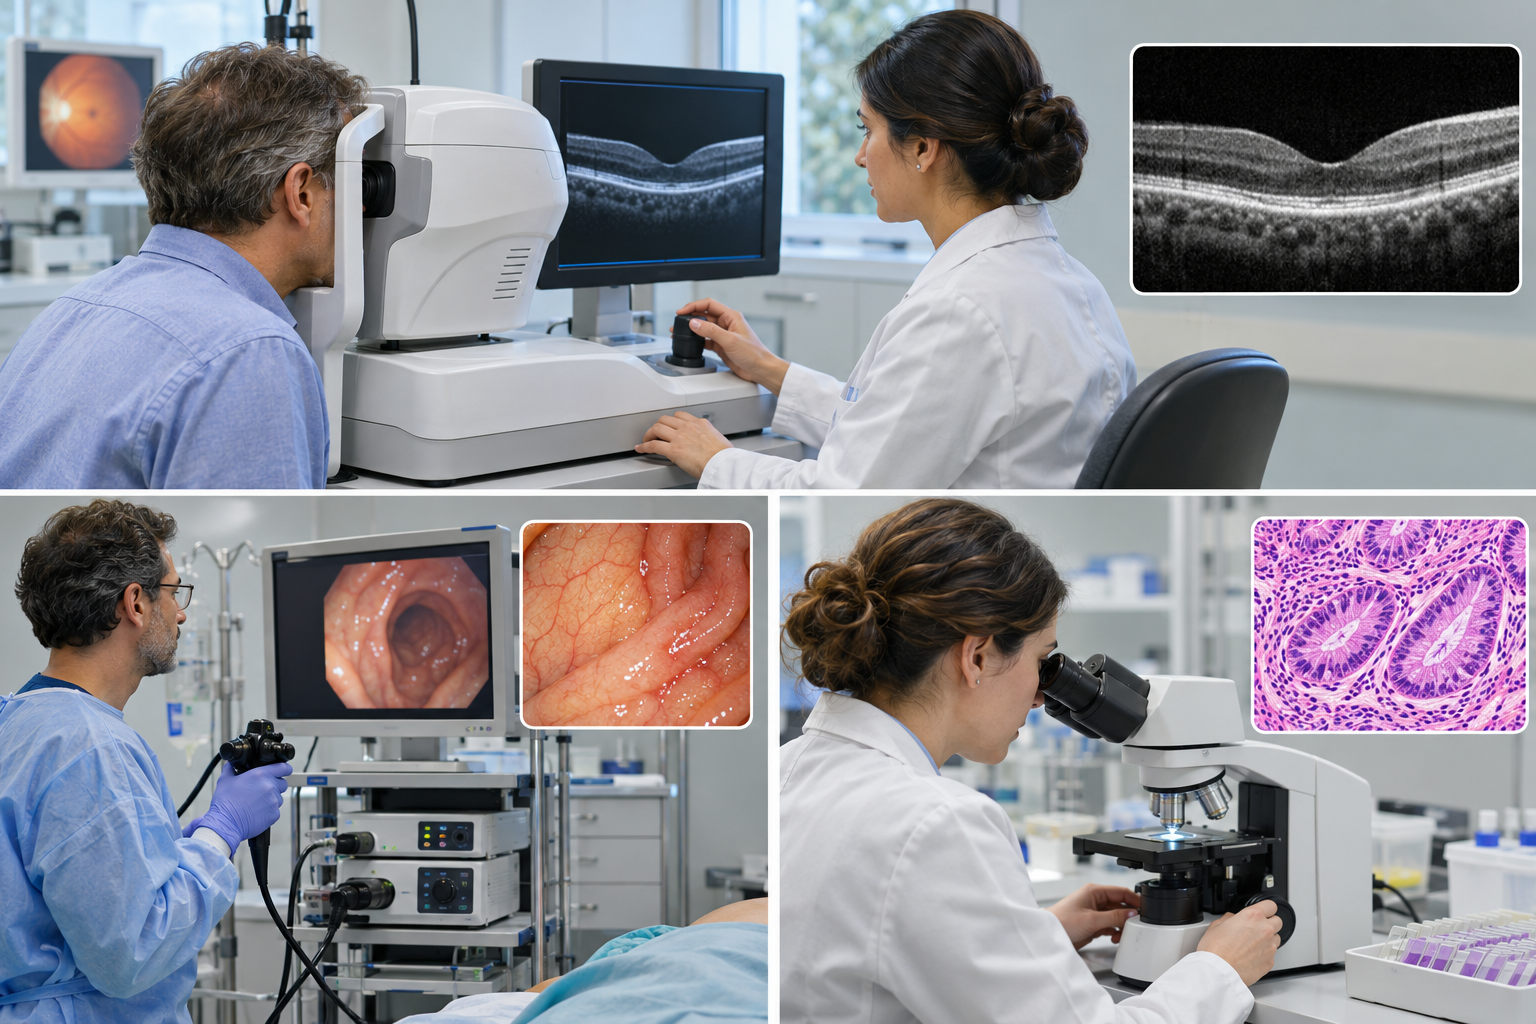
\includegraphics[width=\textwidth,keepaspectratio]{modalities/infographics/optical_realistic.png}
\end{center}
\begin{center}\footnotesize Optical methods include OCT, endoscopy, and microscopy; they reveal structure at different scales, while tissue scattering limits depth. AI-generated illustration; all image panels are illustrative.\end{center}

\section{Overview}
Optical imaging encompasses medical imaging techniques that use ultraviolet, visible, near-infrared, or infrared light to visualize anatomical structures, tissue microarchitecture, vascular networks, cellular morphology, biochemical composition, and physiological activity.

Unlike X-ray, CT, and nuclear medicine, optical imaging does not use ionizing radiation. Its principal limitation is the absorption and scattering of light within biological tissues, which restricts imaging penetration depth. Optical imaging can provide exceptionally high spatial resolution, from macroscopic anatomical visualization to subcellular characterization.

\begin{center}
\begin{tabular}{@{}p{0.32\textwidth}p{0.31\textwidth}p{0.29\textwidth}@{}}
\toprule
\textbf{Imaging modality} & \textbf{Physical principle} & \textbf{Primary clinical application} \\
\midrule
Autofluorescence imaging & Endogenous tissue fluorescence & Retinal and epithelial abnormalities \\
Confocal microscopy & Spatially filtered optical detection & Cellular and tissue microstructure \\
Conventional medical photography & Visible light reflection & Dermatology, wound assessment \\
Dermoscopy & Magnified polarized or nonpolarized light & Skin lesion characterization \\
Diffuse optical tomography (DOT) & Diffuse photon propagation & Functional tissue imaging \\
Digital optical microscopy & Magnified transmitted or reflected light & Histopathology and cytopathology \\
Endoscopy & Direct optical visualization & Gastrointestinal and respiratory diseases \\
Fluorescence angiography & Fluorescent dye excitation and emission & Retinal and vascular imaging \\
Fluorescence imaging & Endogenous or exogenous fluorescence & Tumor and tissue visualization \\
Fluorescence lifetime imaging & Fluorescence decay characteristics & Tissue metabolic characterization \\
Functional NIRS (fNIRS) & Hemodynamic optical signal variation & Functional brain imaging \\
Fundus photography & Retinal light reflection & Retinal diseases \\
Hyperspectral imaging & Wavelength-dependent tissue reflectance & Tissue oxygenation and characterization \\
Infrared thermography & Naturally emitted infrared radiation & Surface temperature distribution \\
Laser speckle contrast imaging & Speckle variation caused by blood flow & Microcirculatory assessment \\
Multiphoton microscopy & Nonlinear optical excitation & Cellular and extracellular structure \\
Narrow-band imaging (NBI) & Wavelength-selective illumination & Epithelial and vascular abnormalities \\
Near-infrared spectroscopy (NIRS) & Wavelength-dependent optical absorption & Tissue oxygenation \\
OCT angiography (OCTA) & Motion-dependent optical signal variation & Retinal microvascular imaging \\
Optical coherence tomography (OCT) & Low-coherence interferometry & Ophthalmology, cardiology \\
Photoacoustic imaging & Optical absorption and acoustic detection & Vascular and functional imaging \\
Raman spectroscopy and imaging & Inelastic photon scattering & Molecular tissue characterization \\
Reflectance confocal microscopy & Backscattered light & Dermatological imaging \\
Second-harmonic generation imaging & Nonlinear frequency conversion & Collagen and fibrous tissue \\
\bottomrule
\end{tabular}
\end{center}

Optical imaging should be treated as a family of distinct modalities, rather than as a single technique. The catalogue includes ophthalmic imaging, endoscopy, dermatology, digital pathology, and other optical methods. Some findings are nonspecific, and several applications remain investigational.

\section{Where optical imaging is used}
The following numbered entries present examples of optical findings and techniques. Optical appearance depends on illumination, wavelength, acquisition geometry, instrument settings, and tissue properties; many findings require clinical or histopathological correlation.

\subsection{Retinal diseases}
\begin{enumerate}[leftmargin=*,itemsep=0.45em,topsep=0.4em]
\item \textbf{Best vitelliform macular dystrophy.} Useful imaging findings include: OCT, autofluorescence. Characteristic Imaging Findings: Vitelliform subretinal deposits.
\item \textbf{Branch retinal artery occlusion.} Useful imaging findings include: OCT, fundus photography. Characteristic Imaging Findings: Sectoral retinal ischemic abnormalities.
\item \textbf{Central retinal artery occlusion.} Useful imaging findings include: Fundus photography, OCT. Characteristic Imaging Findings: Retinal whitening and acute inner retinal hyperreflectivity.
\item \textbf{Central serous chorioretinopathy.} Useful imaging findings include: OCT. Characteristic Imaging Findings: Serous neurosensory retinal detachment.
\item \textbf{Choroidal neovascularization.} Useful imaging findings include: OCTA, fluorescein angiography. Characteristic Imaging Findings: Abnormal vascular network beneath or within the retina.
\item \textbf{Coats disease.} Coats disease is an abnormal retinal telangiectasia with leakage; imaging assesses exudation and retinal detachment. Useful imaging findings include: Fundus photography, angiography. Characteristic Imaging Findings: Retinal telangiectasia and exudation.
\item \textbf{Diabetic macular edema.} Useful imaging findings include: OCT. Characteristic Imaging Findings: Retinal thickening and intraretinal cystic spaces.
\item \textbf{Diabetic retinopathy.} Useful imaging findings include: Fundus photography. Characteristic Imaging Findings: Microaneurysms, hemorrhages, hard exudates.
\item \textbf{Dry age-related macular degeneration.} Useful imaging findings include: OCT, fundus photography. Characteristic Imaging Findings: Drusen and retinal pigment epithelial abnormalities.
\item \textbf{Epiretinal membrane.} Useful imaging findings include: OCT. Characteristic Imaging Findings: Hyperreflective membrane along retinal surface.
\item \textbf{Geographic atrophy.} Geographic atrophy is progressive loss of retinal pigment epithelium and outer retina in age-related macular degeneration; imaging maps its extent. Useful imaging findings include: Fundus autofluorescence, OCT. Characteristic Imaging Findings: Reduced autofluorescence and outer retinal atrophy.
\item \textbf{Hydroxychloroquine retinopathy.} Useful imaging findings include: OCT, autofluorescence. Characteristic Imaging Findings: Parafoveal or pericentral outer retinal degeneration.
\item \textbf{Hypertensive retinopathy.} Useful imaging findings include: Fundus photography. Characteristic Imaging Findings: Arteriolar narrowing, hemorrhages and cotton-wool spots.
\item \textbf{Macular hole.} Useful imaging findings include: OCT. Characteristic Imaging Findings: Full-thickness or partial-thickness foveal defect.
\item \textbf{Neovascular age-related macular degeneration.} Useful imaging findings include: OCT, OCTA. Characteristic Imaging Findings: Neovascular complexes, subretinal or intraretinal fluid.
\item \textbf{Proliferative diabetic retinopathy.} Useful imaging findings include: Fundus photography, fluorescein angiography. Characteristic Imaging Findings: Retinal neovascularization and vascular leakage.
\item \textbf{Retinal detachment.} Useful imaging findings include: Fundus photography, OCT. Characteristic Imaging Findings: Separation of neurosensory retina from underlying tissue; OCT assesses scanned regions, while peripheral extent requires a dilated retinal examination.
\item \textbf{Retinal tear.} Useful imaging findings include: Wide-field fundus imaging. Characteristic Imaging Findings: Discontinuity in peripheral retinal tissue.
\item \textbf{Retinal telangiectasia.} Useful imaging findings include: OCTA, fluorescein angiography. Characteristic Imaging Findings: Abnormal dilated retinal capillaries.
\item \textbf{Retinal vasculitis.} Useful imaging findings include: Fluorescein angiography. Characteristic Imaging Findings: Vascular staining and leakage.
\item \textbf{Retinal vein occlusion.} Useful imaging findings include: Fundus photography, fluorescein angiography. Characteristic Imaging Findings: Retinal hemorrhages, venous dilatation and delayed drainage.
\item \textbf{Retinitis pigmentosa.} Useful imaging findings include: OCT, fundus autofluorescence. Characteristic Imaging Findings: Outer retinal degeneration and characteristic autofluorescent abnormalities.
\item \textbf{Retinopathy of prematurity.} Useful imaging findings include: Wide-field retinal imaging. Characteristic Imaging Findings: Abnormal peripheral retinal vascular development.
\item \textbf{Stargardt disease.} Stargardt disease is an inherited macular dystrophy associated with lipofuscin accumulation; imaging assesses characteristic deposits and atrophy. Useful imaging findings include: Fundus autofluorescence, OCT. Characteristic Imaging Findings: Abnormal lipofuscin distribution and macular atrophy.
\item \textbf{Vitreomacular traction.} Useful imaging findings include: OCT. Characteristic Imaging Findings: Persistent vitreous attachment with foveal distortion.
\item \textbf{Vitreous hemorrhage.} Useful imaging findings include: Fundus photography. Characteristic Imaging Findings: Obscured retinal visualization from intraocular blood.
\end{enumerate}

\subsection{Glaucoma and optic nerve disorders}
\begin{enumerate}[leftmargin=*,itemsep=0.45em,topsep=0.4em]
\item \textbf{Compressive optic neuropathy.} Useful imaging findings include: OCT. Characteristic Imaging Findings: Characteristic patterns of ganglion cell and nerve fiber loss.
\item \textbf{Ischemic optic neuropathy.} Useful imaging findings include: OCT, fundus photography. Characteristic Imaging Findings: Optic disc edema followed by sectoral atrophy.
\item \textbf{Juvenile glaucoma.} Useful imaging findings include: OCT. Characteristic Imaging Findings: Optic nerve head and retinal nerve fiber abnormalities.
\item \textbf{Normal-tension glaucoma.} Useful imaging findings include: OCT. Characteristic Imaging Findings: Retinal nerve fiber and ganglion cell loss.
\item \textbf{Optic atrophy.} Useful imaging findings include: OCT, fundus photography. Characteristic Imaging Findings: Optic disc pallor and nerve fiber loss.
\item \textbf{Optic disc drusen.} Useful imaging findings include: Enhanced-depth OCT. Characteristic Imaging Findings: Characteristic buried or superficial optic nerve head deposits.
\item \textbf{Optic neuritis.} Useful imaging findings include: OCT. Characteristic Imaging Findings: Acute swelling or subsequent retinal nerve fiber thinning.
\item \textbf{Papilledema.} Useful imaging findings include: OCT, fundus photography. Characteristic Imaging Findings: Optic disc swelling and increased nerve fiber thickness.
\item \textbf{Pigmentary glaucoma.} Useful imaging findings include: Slit-lamp imaging, OCT. Characteristic Imaging Findings: Pigment deposition and glaucomatous damage.
\item \textbf{Primary angle-closure glaucoma.} Useful imaging findings include: Anterior segment OCT, optic nerve OCT. Characteristic Imaging Findings: Narrow anterior chamber angle and glaucomatous structural damage.
\item \textbf{Primary open-angle glaucoma.} Useful imaging findings include: OCT. Characteristic Imaging Findings: Retinal nerve fiber layer thinning.
\item \textbf{Pseudoexfoliative glaucoma.} Useful imaging findings include: Slit-lamp imaging, OCT. Characteristic Imaging Findings: Pseudoexfoliative material and optic nerve damage.
\end{enumerate}
Optical imaging can quantify structural glaucomatous damage, but glaucoma diagnosis also requires clinical assessment, intraocular pressure measurements, visual field testing, and, where appropriate, gonioscopy.

\subsection{Corneal and anterior segment disorders}
\begin{enumerate}[leftmargin=*,itemsep=0.45em,topsep=0.4em]
\item \textbf{Acanthamoeba keratitis.} Acanthamoeba keratitis is a corneal infection that can cause severe pain and stromal injury; confocal findings can support, but do not replace, microbiological assessment. Useful imaging findings include: Confocal microscopy. Characteristic Imaging Findings: Characteristic cyst-like structures.
\item \textbf{Anterior uveitis.} Anterior uveitis is inflammation within the anterior eye; slit-lamp examination identifies cells and flare. Useful imaging findings include: Slit-lamp imaging. Characteristic Imaging Findings: Inflammatory cells and flare.
\item \textbf{Bacterial keratitis.} Bacterial keratitis is corneal infection; imaging documents the infiltrate and epithelial defect, while microbiology may guide treatment. Useful imaging findings include: Slit-lamp imaging. Characteristic Imaging Findings: Corneal infiltrate and epithelial defect.
\item \textbf{Cataract.} Useful imaging findings include: Slit-lamp photography, Scheimpflug imaging. Characteristic Imaging Findings: Lens opacity.
\item \textbf{Corneal dystrophy.} Useful imaging findings include: Confocal microscopy, OCT. Characteristic Imaging Findings: Abnormal corneal deposits.
\item \textbf{Corneal edema.} Useful imaging findings include: OCT. Characteristic Imaging Findings: Increased corneal thickness.
\item \textbf{Corneal scarring.} Useful imaging findings include: OCT. Characteristic Imaging Findings: Abnormal stromal reflectivity.
\item \textbf{Corneal ulcer.} Useful imaging findings include: Slit-lamp imaging, OCT. Characteristic Imaging Findings: Epithelial defect and stromal inflammation.
\item \textbf{Dry eye disease.} Dry eye disease reflects tear-film instability or inadequate tear production; optical assessment examines tear-film and ocular-surface changes. Useful imaging findings include: Optical tear film imaging. Characteristic Imaging Findings: Tear film instability and altered tear meniscus.
\item \textbf{Fuchs endothelial dystrophy.} Fuchs endothelial dystrophy is a progressive corneal endothelial disorder; imaging assesses guttata, cell loss, and corneal edema. Useful imaging findings include: Specular microscopy. Characteristic Imaging Findings: Endothelial cell abnormalities and guttata.
\item \textbf{Fungal keratitis.} Fungal keratitis is corneal infection that may involve deeper stromal tissue; confocal findings can help target microbiological sampling. Useful imaging findings include: Confocal microscopy. Characteristic Imaging Findings: Possible filamentous fungal structures.
\item \textbf{Herpes simplex keratitis.} Herpes simplex keratitis is viral corneal infection; fluorescein-assisted examination can show characteristic epithelial lesions. Useful imaging findings include: Fluorescein-assisted slit-lamp imaging. Characteristic Imaging Findings: Dendritic epithelial lesions.
\item \textbf{Hyphema.} Hyphema is blood in the anterior chamber, usually after trauma; imaging documents its extent when direct examination is limited. Useful imaging findings include: Anterior segment photography. Characteristic Imaging Findings: Blood within the anterior chamber.
\item \textbf{Iris melanoma.} Useful imaging findings include: Anterior segment photography, OCT. Characteristic Imaging Findings: Pigmented iris mass with abnormal morphology.
\item \textbf{Keratoconus.} Keratoconus is progressive corneal thinning and irregular steepening; tomography assesses shape and severity. Useful imaging findings include: Corneal tomography, OCT. Characteristic Imaging Findings: Corneal thinning and abnormal curvature.
\item \textbf{Keratoglobus.} Keratoglobus is diffuse corneal thinning with globular protrusion; tomography maps corneal thickness and contour. Useful imaging findings include: Corneal tomography. Characteristic Imaging Findings: Diffuse corneal thinning and protrusion.
\item \textbf{Meibomian gland dysfunction.} Meibomian gland dysfunction impairs the lipid layer of the tear film; infrared meibography can show gland dropout or distortion. Useful imaging findings include: Infrared meibography. Characteristic Imaging Findings: Gland shortening, distortion or dropout.
\item \textbf{Pellucid marginal degeneration.} Useful imaging findings include: Corneal tomography. Characteristic Imaging Findings: Inferior peripheral corneal thinning.
\item \textbf{Posterior capsular opacification.} Useful imaging findings include: Slit-lamp photography. Characteristic Imaging Findings: Opacification of the posterior lens capsule.
\item \textbf{Pterygium.} Pterygium is fibrovascular conjunctival tissue extending onto the cornea; imaging assesses corneal involvement and induced distortion. Useful imaging findings include: Slit-lamp photography, OCT. Characteristic Imaging Findings: Fibrovascular tissue extending onto the cornea.
\end{enumerate}

\subsection{Dermatological malignancies}
\begin{enumerate}[leftmargin=*,itemsep=0.45em,topsep=0.4em]
\item \textbf{Acral melanoma.} Useful imaging findings include: Dermoscopy. Characteristic Imaging Findings: Irregular pigmentation, sometimes parallel ridge pattern.
\item \textbf{Actinic keratosis.} Actinic keratosis is a sun-related keratinocytic lesion with potential for progression; optical examination helps select lesions for biopsy or treatment. Useful imaging findings include: Dermoscopy, confocal microscopy. Characteristic Imaging Findings: Surface keratin and atypical epidermal architecture.
\item \textbf{Amelanotic melanoma.} Useful imaging findings include: Dermoscopy. Characteristic Imaging Findings: Atypical polymorphous vessels.
\item \textbf{Basal cell carcinoma.} Useful imaging findings include: Dermoscopy. Characteristic Imaging Findings: Arborizing vessels, blue-gray structures and ulceration.
\item \textbf{Cutaneous T-cell lymphoma.} Useful imaging findings include: Dermoscopy. Characteristic Imaging Findings: Variable vascular and scaling patterns.
\item \textbf{Dermatofibrosarcoma protuberans.} Useful imaging findings include: Dermoscopy. Characteristic Imaging Findings: Variable pigmentation and vascular abnormalities.
\item \textbf{Extramammary Paget disease.} Useful imaging findings include: Dermoscopy, confocal microscopy. Characteristic Imaging Findings: Atypical intraepidermal cellular structures.
\item \textbf{Lentigo maligna.} Lentigo maligna is melanoma in situ on chronically sun-damaged skin; dermoscopy and confocal microscopy help define suspicious margins. Useful imaging findings include: Dermoscopy, reflectance confocal microscopy. Characteristic Imaging Findings: Irregular follicular pigmentation and atypical melanocytes.
\item \textbf{Malignant melanoma.} Useful imaging findings include: Dermoscopy. Characteristic Imaging Findings: Atypical pigment network and asymmetric structures.
\item \textbf{Merkel cell carcinoma.} Useful imaging findings include: Dermoscopy. Characteristic Imaging Findings: Nonspecific atypical vascular structures.
\item \textbf{Nodular melanoma.} Useful imaging findings include: Dermoscopy. Characteristic Imaging Findings: Atypical vascular and pigmented structures.
\item \textbf{Squamous cell carcinoma.} Useful imaging findings include: Dermoscopy. Characteristic Imaging Findings: Keratin accumulation and abnormal vessels.
\item \textbf{Squamous cell carcinoma in situ.} Useful imaging findings include: Dermoscopy. Characteristic Imaging Findings: Glomerular vessels and scaling.
\item \textbf{Superficial basal cell carcinoma.} Useful imaging findings include: OCT, dermoscopy. Characteristic Imaging Findings: Abnormal superficial epithelial tumor structures.
\end{enumerate}
Histopathological examination remains essential for definitive diagnosis of many cutaneous malignancies.

\subsection{Benign skin lesions}
\begin{enumerate}[leftmargin=*,itemsep=0.45em,topsep=0.4em]
\item \textbf{Angiokeratoma.} Useful imaging findings include: Dermoscopy. Characteristic Imaging Findings: Dark vascular lacunae.
\item \textbf{Blue nevus.} Useful imaging findings include: Dermoscopy. Characteristic Imaging Findings: Homogeneous blue pigmentation.
\item \textbf{Café-au-lait macule.} Useful imaging findings include: Medical photography. Characteristic Imaging Findings: Uniformly pigmented macule.
\item \textbf{Cherry angioma.} Useful imaging findings include: Dermoscopy. Characteristic Imaging Findings: Red vascular lacunae.
\item \textbf{Dermatofibroma.} Useful imaging findings include: Dermoscopy. Characteristic Imaging Findings: Central white scar-like area with peripheral pigmentation.
\item \textbf{Epidermoid cyst.} Useful imaging findings include: Dermoscopy, photography. Characteristic Imaging Findings: Central punctum and superficial structural changes.
\item \textbf{Melanocytic nevus.} Useful imaging findings include: Dermoscopy. Characteristic Imaging Findings: Regular pigment network or globular pattern.
\item \textbf{Milia.} Useful imaging findings include: Dermoscopy. Characteristic Imaging Findings: Small white-yellow keratin-containing structures.
\item \textbf{Molluscum contagiosum.} Useful imaging findings include: Dermoscopy. Characteristic Imaging Findings: Central umbilication and peripheral vessels.
\item \textbf{Pyogenic granuloma.} Useful imaging findings include: Dermoscopy. Characteristic Imaging Findings: Red homogeneous vascular area and possible white collarette.
\item \textbf{Sebaceous hyperplasia.} Useful imaging findings include: Dermoscopy. Characteristic Imaging Findings: Yellow lobules with peripheral vessels.
\item \textbf{Seborrheic keratosis.} Useful imaging findings include: Dermoscopy. Characteristic Imaging Findings: Milia-like cysts and comedo-like openings.
\item \textbf{Solar lentigo.} Useful imaging findings include: Dermoscopy. Characteristic Imaging Findings: Relatively uniform pigmentation.
\item \textbf{Spitz nevus.} Useful imaging findings include: Dermoscopy. Characteristic Imaging Findings: Starburst or other characteristic patterns.
\item \textbf{Viral wart.} Useful imaging findings include: Dermoscopy. Characteristic Imaging Findings: Papillary structures and thrombosed capillaries.
\end{enumerate}

\subsection{Inflammatory and infectious skin diseases}
\begin{enumerate}[leftmargin=*,itemsep=0.45em,topsep=0.4em]
\item \textbf{Acne vulgaris.} Useful imaging findings include: Medical photography. Characteristic Imaging Findings: Comedones, papules, pustules and nodules.
\item \textbf{Atopic dermatitis.} Useful imaging findings include: Dermoscopy. Characteristic Imaging Findings: Patchy vascular structures and yellow scales.
\item \textbf{Bullous pemphigoid.} Useful imaging findings include: Medical photography. Characteristic Imaging Findings: Tense cutaneous blisters.
\item \textbf{Cutaneous candidiasis.} Useful imaging findings include: Medical photography. Characteristic Imaging Findings: Erythema and satellite lesions.
\item \textbf{Demodicosis.} Useful imaging findings include: Dermoscopy. Characteristic Imaging Findings: Follicular protrusions and abnormalities.
\item \textbf{Discoid lupus erythematosus.} Useful imaging findings include: Dermoscopy. Characteristic Imaging Findings: Follicular plugging and pigmentary abnormalities.
\item \textbf{Erythrasma.} Useful imaging findings include: Wood lamp imaging. Characteristic Imaging Findings: Coral-red fluorescence.
\item \textbf{Hidradenitis suppurativa.} Useful imaging findings include: Medical photography. Characteristic Imaging Findings: Nodules, draining tunnels and scarring.
\item \textbf{Lichen planus.} Useful imaging findings include: Dermoscopy. Characteristic Imaging Findings: Wickham striae.
\item \textbf{Melasma.} Useful imaging findings include: Dermoscopy. Characteristic Imaging Findings: Reticulated facial pigmentation.
\item \textbf{Pemphigus vulgaris.} Useful imaging findings include: Medical photography. Characteristic Imaging Findings: Flaccid blisters and erosions.
\item \textbf{Pityriasis versicolor.} Useful imaging findings include: Wood lamp imaging, dermoscopy. Characteristic Imaging Findings: Variable fluorescence and fine scaling.
\item \textbf{Porphyria cutanea tarda.} Useful imaging findings include: Medical photography. Characteristic Imaging Findings: Blistering and skin fragility.
\item \textbf{Psoriasis.} Useful imaging findings include: Dermoscopy. Characteristic Imaging Findings: Regularly distributed dotted vessels and white scales.
\item \textbf{Rosacea.} Useful imaging findings include: Dermoscopy. Characteristic Imaging Findings: Polygonal vascular networks.
\item \textbf{Scabies.} Useful imaging findings include: Dermoscopy. Characteristic Imaging Findings: Mite-associated triangular structure and burrow.
\item \textbf{Seborrheic dermatitis.} Useful imaging findings include: Dermoscopy. Characteristic Imaging Findings: Yellow scaling and irregular vascular patterns.
\item \textbf{Tinea capitis.} Useful imaging findings include: Trichoscopy. Characteristic Imaging Findings: Comma hairs, corkscrew hairs and broken hairs.
\item \textbf{Tinea corporis.} Useful imaging findings include: Dermoscopy. Characteristic Imaging Findings: Peripheral scaling.
\item \textbf{Vitiligo.} Useful imaging findings include: Wood lamp imaging. Characteristic Imaging Findings: Accentuated depigmented regions.
\end{enumerate}

\subsection{Hair and nail disorders}
\begin{enumerate}[leftmargin=*,itemsep=0.45em,topsep=0.4em]
\item \textbf{Alopecia areata.} Useful imaging findings include: Trichoscopy. Characteristic Imaging Findings: Yellow dots, black dots and exclamation mark hairs.
\item \textbf{Androgenetic alopecia.} Useful imaging findings include: Trichoscopy. Characteristic Imaging Findings: Hair shaft diameter variability and miniaturization.
\item \textbf{Beau lines.} Useful imaging findings include: Medical photography. Characteristic Imaging Findings: Transverse nail plate depressions.
\item \textbf{Discoid lupus-associated alopecia.} Useful imaging findings include: Trichoscopy. Characteristic Imaging Findings: Follicular plugging and scarring.
\item \textbf{Frontal fibrosing alopecia.} Useful imaging findings include: Trichoscopy. Characteristic Imaging Findings: Scarring and follicular opening loss.
\item \textbf{Lichen planopilaris.} Useful imaging findings include: Trichoscopy. Characteristic Imaging Findings: Perifollicular scaling and loss of follicular openings.
\item \textbf{Nail melanoma.} Useful imaging findings include: Onychoscopy. Characteristic Imaging Findings: Irregular longitudinal pigmentation.
\item \textbf{Nail psoriasis.} Useful imaging findings include: Onychoscopy. Characteristic Imaging Findings: Pitting, oil-drop changes and onycholysis.
\item \textbf{Nailfold microangiopathy.} Useful imaging findings include: Capillaroscopy. Characteristic Imaging Findings: Abnormal capillary morphology.
\item \textbf{Onycholysis.} Useful imaging findings include: Medical photography. Characteristic Imaging Findings: Separation of nail plate from nail bed.
\item \textbf{Onychomycosis.} Useful imaging findings include: Onychoscopy. Characteristic Imaging Findings: Irregular distal changes and longitudinal spikes.
\item \textbf{Subungual hemorrhage.} Useful imaging findings include: Onychoscopy. Characteristic Imaging Findings: Blood-associated globular pigmentation.
\item \textbf{Telogen effluvium.} Useful imaging findings include: Trichoscopy. Characteristic Imaging Findings: Reduced hair density without marked miniaturization.
\item \textbf{Trichotillomania.} Useful imaging findings include: Trichoscopy. Characteristic Imaging Findings: Broken hairs of varying lengths.
\end{enumerate}

\subsection{Esophageal diseases}
\begin{enumerate}[leftmargin=*,itemsep=0.45em,topsep=0.4em]
\item \textbf{Barrett esophagus.} Useful imaging findings include: High-definition endoscopy, NBI. Characteristic Imaging Findings: Salmon-colored columnar mucosa and altered surface architecture.
\item \textbf{Barrett-associated dysplasia.} Useful imaging findings include: NBI, confocal laser endomicroscopy. Characteristic Imaging Findings: Irregular mucosal and microvascular patterns.
\item \textbf{Candida esophagitis.} Useful imaging findings include: Endoscopy. Characteristic Imaging Findings: Adherent white plaques.
\item \textbf{Cytomegalovirus esophagitis.} Useful imaging findings include: Endoscopy. Characteristic Imaging Findings: Frequently large longitudinal ulcers.
\item \textbf{Eosinophilic esophagitis.} Useful imaging findings include: Endoscopy. Characteristic Imaging Findings: Rings, furrows and white exudates.
\item \textbf{Esophageal adenocarcinoma.} Useful imaging findings include: Endoscopy, NBI. Characteristic Imaging Findings: Irregular mucosal mass or ulcerated lesion.
\item \textbf{Esophageal diverticulum.} Useful imaging findings include: Endoscopy. Characteristic Imaging Findings: Abnormal luminal outpouching.
\item \textbf{Esophageal squamous cell carcinoma.} Useful imaging findings include: NBI, chromoendoscopy. Characteristic Imaging Findings: Abnormal intrapapillary capillary loops.
\item \textbf{Esophageal stricture.} Useful imaging findings include: Endoscopy. Characteristic Imaging Findings: Luminal narrowing.
\item \textbf{Esophageal varices.} Useful imaging findings include: Endoscopy. Characteristic Imaging Findings: Dilated submucosal veins.
\item \textbf{Gastroesophageal reflux disease.} Useful imaging findings include: White-light endoscopy. Characteristic Imaging Findings: Esophageal mucosal breaks in erosive disease.
\item \textbf{Herpes simplex esophagitis.} Useful imaging findings include: Endoscopy. Characteristic Imaging Findings: Multiple small ulcerations.
\item \textbf{Mallory--Weiss tear.} Useful imaging findings include: Endoscopy. Characteristic Imaging Findings: Linear mucosal laceration.
\item \textbf{Reflux esophagitis.} Useful imaging findings include: Endoscopy. Characteristic Imaging Findings: Erythema and mucosal erosions.
\item \textbf{Schatzki ring.} Useful imaging findings include: Endoscopy. Characteristic Imaging Findings: Circumferential mucosal ring.
\end{enumerate}

\subsection{Gastric and duodenal diseases}
\begin{enumerate}[leftmargin=*,itemsep=0.45em,topsep=0.4em]
\item \textbf{Acute gastritis.} Useful imaging findings include: Endoscopy. Characteristic Imaging Findings: Erythema, edema and erosions.
\item \textbf{Advanced gastric carcinoma.} Useful imaging findings include: Endoscopy. Characteristic Imaging Findings: Irregular ulcerated or infiltrative mass.
\item \textbf{Celiac disease.} Useful imaging findings include: Endoscopy. Characteristic Imaging Findings: Scalloping and reduced duodenal folds.
\item \textbf{Chronic atrophic gastritis.} Useful imaging findings include: Endoscopy, NBI. Characteristic Imaging Findings: Reduced mucosal folds and visible submucosal vessels.
\item \textbf{Dieulafoy lesion.} Useful imaging findings include: Endoscopy. Characteristic Imaging Findings: Abnormal exposed vessel with possible bleeding.
\item \textbf{Duodenal adenoma.} Useful imaging findings include: Endoscopy, NBI. Characteristic Imaging Findings: Abnormal glandular mucosal lesion.
\item \textbf{Duodenal ulcer.} Useful imaging findings include: Endoscopy. Characteristic Imaging Findings: Duodenal mucosal defect.
\item \textbf{Early gastric carcinoma.} Useful imaging findings include: Magnifying NBI. Characteristic Imaging Findings: Demarcated abnormal vascular or surface architecture.
\item \textbf{Fundic gland polyp.} Useful imaging findings include: Endoscopy. Characteristic Imaging Findings: Small smooth mucosal polyp.
\item \textbf{Gastric adenoma.} Useful imaging findings include: Endoscopy, NBI. Characteristic Imaging Findings: Altered epithelial surface architecture.
\item \textbf{Gastric antral vascular ectasia.} Useful imaging findings include: Endoscopy. Characteristic Imaging Findings: Linear or diffuse ectatic mucosal vessels.
\item \textbf{Gastric dysplasia.} Useful imaging findings include: Magnifying NBI. Characteristic Imaging Findings: Irregular microsurface and microvascular patterns.
\item \textbf{Gastric gastrointestinal stromal tumor.} Useful imaging findings include: Endoscopy. Characteristic Imaging Findings: Subepithelial protrusion.
\item \textbf{Gastric intestinal metaplasia.} Useful imaging findings include: NBI. Characteristic Imaging Findings: Altered mucosal surface and light-blue crest pattern.
\item \textbf{Gastric lymphoma.} Useful imaging findings include: Endoscopy. Characteristic Imaging Findings: Variable ulceration, nodularity or infiltration.
\item \textbf{Gastric ulcer.} Useful imaging findings include: Endoscopy. Characteristic Imaging Findings: Discrete mucosal ulceration.
\item \textbf{Hyperplastic gastric polyp.} Useful imaging findings include: Endoscopy. Characteristic Imaging Findings: Erythematous or lobulated polyp.
\item \textbf{Portal hypertensive gastropathy.} Useful imaging findings include: Endoscopy. Characteristic Imaging Findings: Mosaic-like gastric mucosal pattern.
\end{enumerate}

\subsection{Small intestinal and colorectal diseases}
\begin{enumerate}[leftmargin=*,itemsep=0.45em,topsep=0.4em]
\item \textbf{Angiodysplasia.} Useful imaging findings include: Endoscopy. Characteristic Imaging Findings: Dilated abnormal mucosal vessels.
\item \textbf{Colonic diverticulosis.} Useful imaging findings include: Colonoscopy. Characteristic Imaging Findings: Diverticular openings.
\item \textbf{Colorectal adenoma.} Useful imaging findings include: NBI, chromoendoscopy. Characteristic Imaging Findings: Abnormal mucosal pit and vascular architecture.
\item \textbf{Colorectal carcinoma.} Useful imaging findings include: Colonoscopy. Characteristic Imaging Findings: Irregular ulcerated or obstructing mass.
\item \textbf{Crohn disease.} Useful imaging findings include: Endoscopy, capsule endoscopy. Characteristic Imaging Findings: Aphthous ulcers, longitudinal ulcerations and cobblestoning.
\item \textbf{Early colorectal carcinoma.} Useful imaging findings include: Magnifying endoscopy. Characteristic Imaging Findings: Markedly abnormal surface and vascular patterns.
\item \textbf{Familial adenomatous polyposis.} Useful imaging findings include: Colonoscopy. Characteristic Imaging Findings: Numerous colorectal adenomas.
\item \textbf{Hyperplastic colorectal polyp.} Useful imaging findings include: NBI. Characteristic Imaging Findings: Generally regular epithelial and vascular patterns.
\item \textbf{Internal hemorrhoids.} Useful imaging findings include: Anoscopy, endoscopy. Characteristic Imaging Findings: Enlarged hemorrhoidal vascular cushions.
\item \textbf{Ischemic colitis.} Useful imaging findings include: Colonoscopy. Characteristic Imaging Findings: Segmental edema, hemorrhage and mucosal ulceration.
\item \textbf{Juvenile polyposis syndrome.} Useful imaging findings include: Colonoscopy. Characteristic Imaging Findings: Multiple characteristic polyps.
\item \textbf{Microscopic colitis.} Useful imaging findings include: Colonoscopy with biopsy. Characteristic Imaging Findings: Frequently normal macroscopic mucosa.
\item \textbf{NSAID-associated enteropathy.} Useful imaging findings include: Capsule endoscopy. Characteristic Imaging Findings: Erosions, ulcerations and possible diaphragm-like strictures.
\item \textbf{Peutz--Jeghers syndrome.} Useful imaging findings include: Endoscopy. Characteristic Imaging Findings: Multiple gastrointestinal polyps.
\item \textbf{Pseudomembranous colitis.} Useful imaging findings include: Colonoscopy. Characteristic Imaging Findings: Adherent yellow-white pseudomembranes.
\item \textbf{Radiation proctitis.} Useful imaging findings include: Endoscopy. Characteristic Imaging Findings: Telangiectasia and mucosal friability.
\item \textbf{Rectal prolapse.} Useful imaging findings include: Medical photography, endoscopy. Characteristic Imaging Findings: Protruding rectal mucosa.
\item \textbf{Sessile serrated lesion.} Useful imaging findings include: Colonoscopy, NBI. Characteristic Imaging Findings: Flat lesion with mucus cap and indistinct margins.
\item \textbf{Small bowel angioectasia.} Useful imaging findings include: Capsule endoscopy. Characteristic Imaging Findings: Focal abnormal vascular structures.
\item \textbf{Small bowel bleeding.} Useful imaging findings include: Capsule endoscopy. Characteristic Imaging Findings: Active bleeding or underlying mucosal lesion.
\item \textbf{Small bowel tumor.} Useful imaging findings include: Capsule endoscopy. Characteristic Imaging Findings: Intraluminal mass or mucosal distortion.
\item \textbf{Small bowel ulceration.} Useful imaging findings include: Capsule endoscopy. Characteristic Imaging Findings: Discrete mucosal defects.
\item \textbf{Solitary rectal ulcer syndrome.} Useful imaging findings include: Endoscopy. Characteristic Imaging Findings: Rectal ulceration or polypoid mucosal abnormality.
\item \textbf{Ulcerative colitis.} Useful imaging findings include: Colonoscopy. Characteristic Imaging Findings: Continuous mucosal inflammation and friability.
\end{enumerate}

\subsection{Respiratory and upper airway diseases}
\begin{enumerate}[leftmargin=*,itemsep=0.45em,topsep=0.4em]
\item \textbf{Airway foreign body.} Useful imaging findings include: Bronchoscopy. Characteristic Imaging Findings: Direct visualization of foreign material.
\item \textbf{Bronchial carcinoid.} Useful imaging findings include: Bronchoscopy. Characteristic Imaging Findings: Smooth, frequently hypervascular endobronchial lesion.
\item \textbf{Bronchial dysplasia.} Useful imaging findings include: Autofluorescence imaging. Characteristic Imaging Findings: Reduced or altered mucosal fluorescence.
\item \textbf{Bronchial squamous cell carcinoma.} Useful imaging findings include: Autofluorescence bronchoscopy. Characteristic Imaging Findings: Abnormal epithelial fluorescence.
\item \textbf{Bronchial stenosis.} Useful imaging findings include: Bronchoscopy. Characteristic Imaging Findings: Reduced bronchial lumen diameter.
\item \textbf{Chronic rhinosinusitis.} Useful imaging findings include: Nasal endoscopy. Characteristic Imaging Findings: Mucosal inflammation, edema and secretions.
\item \textbf{Endobronchial lung carcinoma.} Useful imaging findings include: Bronchoscopy. Characteristic Imaging Findings: Irregular obstructing bronchial mass.
\item \textbf{Endobronchial tuberculosis.} Useful imaging findings include: Bronchoscopy. Characteristic Imaging Findings: Ulceration, inflammatory changes or stenosis.
\item \textbf{Laryngeal carcinoma.} Useful imaging findings include: NBI, laryngoscopy. Characteristic Imaging Findings: Irregular epithelial lesion and abnormal vascularity.
\item \textbf{Laryngeal papillomatosis.} Useful imaging findings include: Laryngoscopy. Characteristic Imaging Findings: Multiple papillomatous lesions.
\item \textbf{Nasal polyposis.} Useful imaging findings include: Nasal endoscopy. Characteristic Imaging Findings: Polypoid lesions within nasal cavity.
\item \textbf{Nasopharyngeal carcinoma.} Useful imaging findings include: Nasopharyngoscopy. Characteristic Imaging Findings: Abnormal nasopharyngeal mass.
\item \textbf{Subglottic stenosis.} Useful imaging findings include: Laryngoscopy. Characteristic Imaging Findings: Narrowing below vocal folds.
\item \textbf{Tracheal stenosis.} Useful imaging findings include: Bronchoscopy. Characteristic Imaging Findings: Tracheal luminal narrowing.
\item \textbf{Tracheobronchomalacia.} Useful imaging findings include: Dynamic bronchoscopy. Characteristic Imaging Findings: Excessive expiratory airway collapse.
\item \textbf{Vocal cord nodule.} Useful imaging findings include: Laryngoscopy. Characteristic Imaging Findings: Nodular vocal fold lesion.
\item \textbf{Vocal cord paralysis.} Useful imaging findings include: Video laryngoscopy. Characteristic Imaging Findings: Abnormal vocal fold movement.
\item \textbf{Vocal cord polyp.} Useful imaging findings include: Laryngoscopy. Characteristic Imaging Findings: Localized polypoid lesion.
\end{enumerate}

\subsection{Cardiovascular diseases}
Intravascular optical coherence tomography provides high-resolution visualization of coronary arterial microstructure.
\begin{enumerate}[leftmargin=*,itemsep=0.45em,topsep=0.4em]
\item \textbf{Calcified coronary plaque.} Useful imaging findings include: OCT. Characteristic Imaging Findings: Low-signal region with sharply defined borders.
\item \textbf{Coronary arterial thrombosis.} Useful imaging findings include: OCT. Characteristic Imaging Findings: Intraluminal thrombotic material.
\item \textbf{Coronary artery dissection.} Useful imaging findings include: OCT. Characteristic Imaging Findings: Intimal disruption or intramural hematoma.
\item \textbf{Coronary atherosclerosis.} Useful imaging findings include: Intravascular OCT. Characteristic Imaging Findings: Atherosclerotic plaque within arterial wall.
\item \textbf{Coronary calcified nodule.} Useful imaging findings include: OCT. Characteristic Imaging Findings: Protruding irregular calcific structure.
\item \textbf{Coronary plaque erosion.} Useful imaging findings include: OCT. Characteristic Imaging Findings: Thrombus over apparently intact plaque surface.
\item \textbf{Coronary plaque rupture.} Useful imaging findings include: OCT. Characteristic Imaging Findings: Fibrous cap discontinuity and plaque cavity.
\item \textbf{Fibrous coronary plaque.} Useful imaging findings include: OCT. Characteristic Imaging Findings: Relatively homogeneous signal-rich tissue.
\item \textbf{In-stent restenosis.} Useful imaging findings include: OCT. Characteristic Imaging Findings: Tissue proliferation within stented segment.
\item \textbf{Lipid-rich coronary plaque.} Useful imaging findings include: OCT. Characteristic Imaging Findings: Low-signal region with diffuse borders.
\item \textbf{Neoatherosclerosis.} Useful imaging findings include: OCT. Characteristic Imaging Findings: Atherosclerotic transformation of neointimal tissue.
\item \textbf{Spontaneous coronary artery dissection.} Useful imaging findings include: OCT. Characteristic Imaging Findings: False lumen or intramural hematoma.
\item \textbf{Stent malapposition.} Useful imaging findings include: OCT. Characteristic Imaging Findings: Separation of stent struts from arterial wall.
\item \textbf{Stent thrombosis.} Useful imaging findings include: OCT. Characteristic Imaging Findings: Thrombotic material associated with stent.
\item \textbf{Stent underexpansion.} Useful imaging findings include: OCT. Characteristic Imaging Findings: Inadequate stent lumen area.
\item \textbf{Thin-cap fibroatheroma.} Useful imaging findings include: OCT. Characteristic Imaging Findings: Lipid-rich plaque with thin fibrous cap.
\end{enumerate}

\subsection{Microvascular and connective tissue disorders}
\begin{enumerate}[leftmargin=*,itemsep=0.45em,topsep=0.4em]
\item \textbf{Dermatomyositis.} Useful imaging findings include: Nailfold capillaroscopy. Characteristic Imaging Findings: Abnormal capillary dilatation and dropout.
\item \textbf{Diabetic microangiopathy.} Useful imaging findings include: Capillaroscopy. Characteristic Imaging Findings: Altered microvascular morphology.
\item \textbf{Microvascular dysfunction.} Useful imaging findings include: Laser Doppler imaging. Characteristic Imaging Findings: Abnormal microcirculatory response.
\item \textbf{Mixed connective tissue disease.} Useful imaging findings include: Nailfold capillaroscopy. Characteristic Imaging Findings: Scleroderma-like microvascular abnormalities.
\item \textbf{Peripheral arterial insufficiency.} Useful imaging findings include: Laser speckle contrast imaging. Characteristic Imaging Findings: Reduced superficial tissue perfusion.
\item \textbf{Primary Raynaud phenomenon.} Useful imaging findings include: Nailfold capillaroscopy. Characteristic Imaging Findings: Typically preserved capillary architecture.
\item \textbf{Secondary Raynaud phenomenon.} Useful imaging findings include: Nailfold capillaroscopy. Characteristic Imaging Findings: Structural microvascular abnormalities.
\item \textbf{Systemic lupus erythematosus.} Useful imaging findings include: Nailfold capillaroscopy. Characteristic Imaging Findings: Variable nonspecific capillary abnormalities.
\item \textbf{Systemic sclerosis.} Useful imaging findings include: Nailfold capillaroscopy. Characteristic Imaging Findings: Giant capillaries, hemorrhages and capillary loss.
\item \textbf{Tissue reperfusion abnormality.} Useful imaging findings include: Laser speckle imaging. Characteristic Imaging Findings: Reduced or heterogeneous microvascular flow.
\end{enumerate}

\subsection{Neurological and functional brain disorders}
Functional optical imaging primarily measures cerebral hemodynamic changes rather than direct neuronal electrical activity.
\begin{enumerate}[leftmargin=*,itemsep=0.45em,topsep=0.4em]
\item \textbf{Alzheimer disease.} Useful imaging findings include: fNIRS. Characteristic Imaging Findings: Altered cortical activation during cognitive tasks.
\item \textbf{Attention-deficit hyperactivity disorder.} Useful imaging findings include: fNIRS. Characteristic Imaging Findings: Altered prefrontal activation patterns in research studies.
\item \textbf{Autism spectrum disorder.} Useful imaging findings include: fNIRS. Characteristic Imaging Findings: Reported differences in cortical functional responses.
\item \textbf{Cerebral autoregulatory dysfunction.} Useful imaging findings include: NIRS. Characteristic Imaging Findings: Abnormal relationship between systemic pressure and cerebral oxygenation.
\item \textbf{Cerebral ischemia.} Useful imaging findings include: NIRS. Characteristic Imaging Findings: Reduced regional cerebral oxygenation.
\item \textbf{Disorders of consciousness.} Useful imaging findings include: fNIRS. Characteristic Imaging Findings: Possible stimulus-associated cortical responses.
\item \textbf{Epilepsy.} Useful imaging findings include: fNIRS. Characteristic Imaging Findings: Seizure-associated hemodynamic changes.
\item \textbf{Major depressive disorder.} Useful imaging findings include: fNIRS. Characteristic Imaging Findings: Reported abnormalities in prefrontal hemodynamic responses.
\item \textbf{Neonatal hypoxic-ischemic encephalopathy.} Useful imaging findings include: NIRS. Characteristic Imaging Findings: Abnormal cerebral oxygenation and extraction patterns.
\item \textbf{Parkinson disease.} Useful imaging findings include: fNIRS. Characteristic Imaging Findings: Altered motor cortical activation.
\item \textbf{Schizophrenia.} Useful imaging findings include: fNIRS. Characteristic Imaging Findings: Altered cortical activation during cognitive tasks.
\item \textbf{Stroke rehabilitation.} Useful imaging findings include: fNIRS. Characteristic Imaging Findings: Changes in motor cortical activation.
\item \textbf{Traumatic brain injury.} Useful imaging findings include: NIRS. Characteristic Imaging Findings: Possible cerebral oxygenation abnormalities.
\end{enumerate}
Most neurological disease classification using fNIRS remains investigational. NIRS has more established applications in physiological monitoring.

\subsection{Breast diseases}
\begin{enumerate}[leftmargin=*,itemsep=0.45em,topsep=0.4em]
\item \textbf{Breast cancer treatment response.} Useful imaging findings include: Diffuse optical spectroscopy. Characteristic Imaging Findings: Changes in tumor-associated hemoglobin and optical properties.
\item \textbf{Breast cyst.} Useful imaging findings include: Optical tomography. Characteristic Imaging Findings: Altered tissue absorption and scattering.
\item \textbf{Breast tumor hypoxia.} Useful imaging findings include: Photoacoustic imaging. Characteristic Imaging Findings: Altered estimated hemoglobin oxygen saturation.
\item \textbf{Ductal carcinoma in situ.} Useful imaging findings include: Optical spectroscopy. Characteristic Imaging Findings: Potential biochemical and structural abnormalities.
\item \textbf{Fibroadenoma.} Useful imaging findings include: Optical tomography. Characteristic Imaging Findings: Variable absorption and scattering characteristics.
\item \textbf{Invasive breast carcinoma.} Useful imaging findings include: Diffuse optical tomography. Characteristic Imaging Findings: Abnormal hemoglobin concentration and optical absorption.
\item \textbf{Invasive lobular carcinoma.} Useful imaging findings include: Diffuse optical imaging. Characteristic Imaging Findings: Variable optical contrast.
\item \textbf{Residual breast carcinoma.} Useful imaging findings include: Fluorescence imaging. Characteristic Imaging Findings: Tumor-associated fluorescent signal using selected agents.
\item \textbf{Tumor-associated angiogenesis.} Useful imaging findings include: Photoacoustic imaging. Characteristic Imaging Findings: Increased or abnormal vascular networks.
\end{enumerate}
Most of these applications are supplementary or investigational. Optical imaging is not an established replacement for mammography, diagnostic ultrasound, MRI, or biopsy.

\subsection{Oral and dental diseases}
\begin{enumerate}[leftmargin=*,itemsep=0.45em,topsep=0.4em]
\item \textbf{Aphthous ulcer.} Useful imaging findings include: Medical photography. Characteristic Imaging Findings: Discrete ulcer with erythematous margin.
\item \textbf{Dental caries.} Useful imaging findings include: Near-infrared transillumination. Characteristic Imaging Findings: Abnormal light transmission through demineralized tissue.
\item \textbf{Dental restoration defects.} Useful imaging findings include: OCT. Characteristic Imaging Findings: Abnormal restoration-tooth interfaces.
\item \textbf{Early enamel demineralization.} Useful imaging findings include: Quantitative light-induced fluorescence. Characteristic Imaging Findings: Reduced enamel autofluorescence.
\item \textbf{Enamel cracks.} Useful imaging findings include: OCT, transillumination. Characteristic Imaging Findings: Linear structural discontinuities.
\item \textbf{Gingivitis.} Useful imaging findings include: Medical photography. Characteristic Imaging Findings: Gingival erythema and swelling.
\item \textbf{Interproximal dental caries.} Useful imaging findings include: Near-infrared imaging. Characteristic Imaging Findings: Abnormal optical shadowing.
\item \textbf{Oral candidiasis.} Useful imaging findings include: Medical photography. Characteristic Imaging Findings: White plaques or erythematous lesions.
\item \textbf{Oral epithelial dysplasia.} Useful imaging findings include: Autofluorescence, confocal microscopy. Characteristic Imaging Findings: Altered fluorescence and epithelial architecture.
\item \textbf{Oral erythroplakia.} Useful imaging findings include: Optical examination. Characteristic Imaging Findings: Abnormal erythematous mucosal lesion.
\item \textbf{Oral leukoplakia.} Useful imaging findings include: Autofluorescence imaging. Characteristic Imaging Findings: Variable reduction in tissue fluorescence.
\item \textbf{Oral lichen planus.} Useful imaging findings include: Medical photography. Characteristic Imaging Findings: Reticular white mucosal striae.
\item \textbf{Oral squamous cell carcinoma.} Useful imaging findings include: Fluorescence imaging, NBI. Characteristic Imaging Findings: Abnormal vascular and epithelial structures.
\item \textbf{Periodontitis.} Useful imaging findings include: OCT, photography. Characteristic Imaging Findings: Periodontal structural abnormalities.
\end{enumerate}

\subsection{Gynecological diseases}
\begin{enumerate}[leftmargin=*,itemsep=0.45em,topsep=0.4em]
\item \textbf{Cervical carcinoma.} Useful imaging findings include: Colposcopy. Characteristic Imaging Findings: Irregular epithelial mass and atypical vessels.
\item \textbf{Cervical ectropion.} Useful imaging findings include: Colposcopy. Characteristic Imaging Findings: Exposed columnar epithelium.
\item \textbf{Cervical intraepithelial neoplasia.} Useful imaging findings include: Colposcopy. Characteristic Imaging Findings: Acetowhite epithelium and abnormal vascular patterns.
\item \textbf{Cervical polyp.} Useful imaging findings include: Colposcopy. Characteristic Imaging Findings: Polypoid cervical lesion.
\item \textbf{Cervicitis.} Useful imaging findings include: Colposcopy. Characteristic Imaging Findings: Erythema and inflammatory changes.
\item \textbf{Endometrial carcinoma.} Useful imaging findings include: Hysteroscopy. Characteristic Imaging Findings: Irregular friable or abnormal endometrial growth.
\item \textbf{Endometrial hyperplasia.} Useful imaging findings include: Hysteroscopy. Characteristic Imaging Findings: Irregular or thickened endometrial appearance.
\item \textbf{Endometrial polyp.} Useful imaging findings include: Hysteroscopy. Characteristic Imaging Findings: Polypoid lesion within uterine cavity.
\item \textbf{Endometriosis.} Useful imaging findings include: Laparoscopy. Characteristic Imaging Findings: Variable superficial pigmented or fibrotic lesions.
\item \textbf{High-grade squamous intraepithelial lesion.} Useful imaging findings include: Colposcopy. Characteristic Imaging Findings: Dense acetowhitening and coarse vascular patterns.
\item \textbf{Intrauterine adhesions.} Useful imaging findings include: Hysteroscopy. Characteristic Imaging Findings: Fibrous bands within uterine cavity.
\item \textbf{Low-grade squamous intraepithelial lesion.} Useful imaging findings include: Colposcopy. Characteristic Imaging Findings: Mild acetowhite changes.
\item \textbf{Submucosal uterine fibroid.} Useful imaging findings include: Hysteroscopy. Characteristic Imaging Findings: Smooth intracavitary protruding mass.
\item \textbf{Vulvar carcinoma.} Useful imaging findings include: Optical examination. Characteristic Imaging Findings: Irregular ulcerated or nodular lesion.
\item \textbf{Vulvar intraepithelial neoplasia.} Useful imaging findings include: Vulvoscopy. Characteristic Imaging Findings: Abnormal epithelial lesions.
\end{enumerate}

\subsection{Urinary tract disorders}
\begin{enumerate}[leftmargin=*,itemsep=0.45em,topsep=0.4em]
\item \textbf{Bladder calculus.} Useful imaging findings include: Cystoscopy. Characteristic Imaging Findings: Direct visualization of stone.
\item \textbf{Bladder carcinoma in situ.} Useful imaging findings include: Blue-light fluorescence cystoscopy. Characteristic Imaging Findings: Abnormal fluorescent mucosal regions.
\item \textbf{Bladder diverticulum.} Useful imaging findings include: Cystoscopy. Characteristic Imaging Findings: Abnormal bladder wall opening.
\item \textbf{Bladder papilloma.} Useful imaging findings include: Cystoscopy. Characteristic Imaging Findings: Papillary lesion.
\item \textbf{Bladder urothelial carcinoma.} Useful imaging findings include: Cystoscopy. Characteristic Imaging Findings: Papillary or solid mucosal tumor.
\item \textbf{Hemorrhagic cystitis.} Useful imaging findings include: Cystoscopy. Characteristic Imaging Findings: Mucosal hemorrhage and inflammation.
\item \textbf{Interstitial cystitis with Hunner lesions.} Useful imaging findings include: Cystoscopy. Characteristic Imaging Findings: Characteristic inflammatory mucosal lesions.
\item \textbf{Recurrent bladder carcinoma.} Useful imaging findings include: Fluorescence cystoscopy. Characteristic Imaging Findings: Fluorescent or structurally abnormal lesions.
\item \textbf{Renal papillary abnormalities.} Useful imaging findings include: Ureteroscopy. Characteristic Imaging Findings: Abnormal renal papillary morphology.
\item \textbf{Upper urinary tract urothelial carcinoma.} Useful imaging findings include: Ureteroscopy. Characteristic Imaging Findings: Papillary or irregular urothelial lesion.
\item \textbf{Ureteral calculus.} Useful imaging findings include: Ureteroscopy. Characteristic Imaging Findings: Direct visualization of calculus.
\item \textbf{Urethral stricture.} Useful imaging findings include: Urethroscopy. Characteristic Imaging Findings: Luminal narrowing.
\end{enumerate}

\subsection{Wounds, burns and tissue perfusion}
\begin{enumerate}[leftmargin=*,itemsep=0.45em,topsep=0.4em]
\item \textbf{Arterial ulcer.} Useful imaging findings include: Hyperspectral imaging. Characteristic Imaging Findings: Reduced superficial tissue oxygenation.
\item \textbf{Deep dermal burn.} Useful imaging findings include: Laser Doppler imaging. Characteristic Imaging Findings: Reduced dermal perfusion.
\item \textbf{Delayed wound healing.} Useful imaging findings include: Serial optical imaging. Characteristic Imaging Findings: Inadequate reduction in wound area.
\item \textbf{Diabetic foot ulcer.} Useful imaging findings include: Medical photography, hyperspectral imaging. Characteristic Imaging Findings: Ulcer morphology and altered tissue oxygenation.
\item \textbf{Early pressure injury.} Useful imaging findings include: Thermal or hyperspectral imaging. Characteristic Imaging Findings: Potential temperature and oxygenation changes.
\item \textbf{Frostbite.} Useful imaging findings include: Laser speckle imaging. Characteristic Imaging Findings: Impaired superficial circulation.
\item \textbf{Full-thickness burn.} Useful imaging findings include: Laser Doppler imaging. Characteristic Imaging Findings: Markedly impaired tissue perfusion.
\item \textbf{Partial-thickness burn.} Useful imaging findings include: Laser Doppler imaging. Characteristic Imaging Findings: Characteristic tissue perfusion patterns.
\item \textbf{Pressure ulcer.} Useful imaging findings include: Medical photography. Characteristic Imaging Findings: Skin breakdown and tissue injury.
\item \textbf{Skin flap ischemia.} Useful imaging findings include: Indocyanine green fluorescence imaging. Characteristic Imaging Findings: Impaired or delayed tissue perfusion.
\item \textbf{Skin graft failure.} Useful imaging findings include: Fluorescence imaging. Characteristic Imaging Findings: Inadequate vascular perfusion.
\item \textbf{Surgical wound dehiscence.} Useful imaging findings include: Medical photography. Characteristic Imaging Findings: Separation of wound edges.
\item \textbf{Tissue necrosis.} Useful imaging findings include: Optical photography, hyperspectral imaging. Characteristic Imaging Findings: Abnormal tissue morphology and oxygenation.
\item \textbf{Venous leg ulcer.} Useful imaging findings include: Medical photography. Characteristic Imaging Findings: Characteristic ulcer morphology and surrounding skin changes.
\item \textbf{Wound-associated infection.} Useful imaging findings include: Bacterial fluorescence imaging. Characteristic Imaging Findings: Fluorescence associated with selected bacterial products.
\end{enumerate}

\subsection{Intraoperative optical imaging}
\begin{enumerate}[leftmargin=*,itemsep=0.45em,topsep=0.4em]
\item \textbf{Anastomotic perfusion impairment.} Useful imaging findings include: Fluorescence angiography. Characteristic Imaging Findings: Reduced fluorescence at anastomotic margins.
\item \textbf{Biliary anatomical abnormalities.} Useful imaging findings include: Fluorescence cholangiography. Characteristic Imaging Findings: Abnormal or altered biliary anatomy.
\item \textbf{Bowel ischemia.} Useful imaging findings include: Indocyanine green fluorescence. Characteristic Imaging Findings: Reduced intestinal perfusion.
\item \textbf{Breast cancer residual tissue.} Useful imaging findings include: Fluorescence imaging. Characteristic Imaging Findings: Tumor-associated fluorescent signal.
\item \textbf{Hepatic malignancy.} Useful imaging findings include: Indocyanine green fluorescence. Characteristic Imaging Findings: Abnormal fluorescence retention or distribution.
\item \textbf{Hepatic metastases.} Useful imaging findings include: Indocyanine green fluorescence. Characteristic Imaging Findings: Possible peritumoral fluorescence.
\item \textbf{High-grade glioma.} Useful imaging findings include: 5-ALA fluorescence imaging. Characteristic Imaging Findings: Fluorescence associated with tumor tissue.
\item \textbf{Ovarian carcinoma.} Useful imaging findings include: Targeted fluorescence imaging. Characteristic Imaging Findings: Fluorescence associated with receptor-positive lesions.
\item \textbf{Parathyroid gland localization.} Useful imaging findings include: Near-infrared autofluorescence. Characteristic Imaging Findings: Characteristic parathyroid fluorescence.
\item \textbf{Peripheral lymphatic dysfunction.} Useful imaging findings include: Indocyanine green lymphography. Characteristic Imaging Findings: Altered lymphatic drainage or dermal backflow.
\item \textbf{Residual malignant glioma.} Useful imaging findings include: Fluorescence-guided surgery. Characteristic Imaging Findings: Persistent tumor-associated fluorescence.
\item \textbf{Sentinel lymph node localization.} Useful imaging findings include: Near-infrared fluorescence imaging. Characteristic Imaging Findings: Visualization of lymphatic drainage pathways.
\end{enumerate}

\subsection{Ex-vivo optical microscopy and digital histopathology}
This section covers optical examination of prepared tissue, blood, or other specimens outside the body (ex vivo), rather than in-vivo imaging of the patient. Digital pathology provides cellular-level or tissue-level information unavailable through conventional radiological modalities.
\begin{enumerate}[leftmargin=*,itemsep=0.45em,topsep=0.4em]
\item \textbf{Acute lymphoblastic leukemia.} Useful imaging findings include: Blood and marrow microscopy. Characteristic Imaging Findings: Abnormal lymphoid blasts.
\item \textbf{Acute myeloid leukemia.} Useful imaging findings include: Blood and marrow microscopy. Characteristic Imaging Findings: Abnormal myeloid blasts.
\item \textbf{Celiac disease.} Useful imaging findings include: Histopathological microscopy. Characteristic Imaging Findings: Villous atrophy and intraepithelial lymphocytosis.
\item \textbf{Colorectal adenocarcinoma.} Useful imaging findings include: Histopathological microscopy. Characteristic Imaging Findings: Malignant gland formation.
\item \textbf{Crohn disease.} Useful imaging findings include: Histopathological microscopy. Characteristic Imaging Findings: Focal inflammation and occasional granulomas.
\item \textbf{Diabetic nephropathy.} Useful imaging findings include: Histopathological microscopy. Characteristic Imaging Findings: Mesangial expansion and nodular glomerulosclerosis.
\item \textbf{Glioblastoma.} Useful imaging findings include: Histopathological microscopy. Characteristic Imaging Findings: Malignant glial cells, necrosis and microvascular proliferation.
\item \textbf{Hepatocellular carcinoma.} Useful imaging findings include: Histopathological microscopy. Characteristic Imaging Findings: Abnormal hepatocellular architecture.
\item \textbf{Hodgkin lymphoma.} Useful imaging findings include: Histopathology, immunohistochemistry. Characteristic Imaging Findings: Characteristic atypical cells within an inflammatory background.
\item \textbf{IgA nephropathy.} Useful imaging findings include: Immunofluorescence microscopy. Characteristic Imaging Findings: Mesangial IgA deposition.
\item \textbf{Invasive ductal breast carcinoma.} Useful imaging findings include: Whole-slide microscopy. Characteristic Imaging Findings: Malignant epithelial cells invading surrounding stroma.
\item \textbf{Invasive lobular breast carcinoma.} Useful imaging findings include: Whole-slide microscopy. Characteristic Imaging Findings: Discohesive tumor cells, often in single-file arrangement.
\item \textbf{Iron deficiency anemia.} Useful imaging findings include: Peripheral blood microscopy. Characteristic Imaging Findings: Microcytic hypochromic erythrocytes.
\item \textbf{Lupus nephritis.} Useful imaging findings include: Immunofluorescence microscopy. Characteristic Imaging Findings: Characteristic multicomponent immune deposition.
\item \textbf{Malaria.} Useful imaging findings include: Blood smear microscopy. Characteristic Imaging Findings: Intraerythrocytic parasites.
\item \textbf{Malignant melanoma.} Useful imaging findings include: Histopathological microscopy. Characteristic Imaging Findings: Atypical melanocytic proliferation.
\item \textbf{Megaloblastic anemia.} Useful imaging findings include: Peripheral blood microscopy. Characteristic Imaging Findings: Macro-ovalocytes and hypersegmented neutrophils.
\item \textbf{Membranous nephropathy.} Useful imaging findings include: Immunofluorescence microscopy. Characteristic Imaging Findings: Granular immune deposits along capillary walls.
\item \textbf{Prostate adenocarcinoma.} Useful imaging findings include: Histopathological microscopy. Characteristic Imaging Findings: Abnormal infiltrative glandular architecture.
\item \textbf{Pulmonary adenocarcinoma.} Useful imaging findings include: Histopathological microscopy. Characteristic Imaging Findings: Malignant glandular or other characteristic growth patterns.
\item \textbf{Renal cell carcinoma.} Useful imaging findings include: Histopathological microscopy. Characteristic Imaging Findings: Subtype-dependent malignant renal cellular morphology.
\item \textbf{Sickle cell disease.} Useful imaging findings include: Peripheral blood microscopy. Characteristic Imaging Findings: Sickle-shaped erythrocytes.
\item \textbf{Squamous cell carcinoma.} Useful imaging findings include: Histopathological microscopy. Characteristic Imaging Findings: Atypical squamous cells with variable keratinization.
\item \textbf{Tuberculosis.} Useful imaging findings include: Fluorescence microscopy. Characteristic Imaging Findings: Fluorescently stained acid-fast bacilli.
\item \textbf{Ulcerative colitis.} Useful imaging findings include: Histopathological microscopy. Characteristic Imaging Findings: Crypt architectural distortion and inflammation.
\end{enumerate}

\subsection{Summary of catalogue}
\begin{center}
\begin{tabular}{@{}p{0.70\textwidth}r@{}}
\toprule
\textbf{Disease category} & \textbf{Entries} \\
\midrule
Benign skin lesions & 15 \\
Breast diseases & 9 \\
Cardiovascular diseases & 16 \\
Corneal and anterior segment disorders & 20 \\
Dermatological malignancies & 14 \\
Esophageal diseases & 15 \\
Ex-vivo optical microscopy and digital histopathology & 25 \\
Gastric and duodenal diseases & 18 \\
Glaucoma and optic nerve disorders & 12 \\
Gynecological diseases & 15 \\
Hair and nail disorders & 14 \\
Inflammatory and infectious skin diseases & 20 \\
Intraoperative optical imaging & 12 \\
Microvascular and connective tissue disorders & 10 \\
Neurological and functional brain disorders & 13 \\
Oral and dental diseases & 14 \\
Respiratory and upper airway diseases & 18 \\
Retinal diseases & 26 \\
Small intestinal and colorectal diseases & 24 \\
Total & 337 \\
Urinary tract disorders & 12 \\
Wounds, burns and tissue perfusion & 15 \\
\bottomrule
\end{tabular}
\end{center}

\subsection{Physical principles of optical imaging}
\paragraph{Electromagnetic wavelength spectrum.}
\begin{longtable}{@{}p{0.40\textwidth}p{0.52\textwidth}@{}}
\toprule
\textbf{Spectral region} & \textbf{Approximate wavelength} \\
\midrule
\endfirsthead
\toprule
\textbf{Spectral region} & \textbf{Approximate wavelength} \\
\midrule
\endhead
Long-wave infrared & 8--14 $\mu$m \\
Mid-wave infrared & 3--5 $\mu$m \\
Near-infrared I & 700--1,000 nm \\
Near-infrared II & 1,000--1,700 nm \\
Short-wave infrared & 1,000--2,500 nm \\
Ultraviolet & 100--400 nm \\
Visible light & 400--700 nm \\
\bottomrule
\end{longtable}
These spectral subdivisions are application-dependent and may overlap.

\paragraph{Light--tissue interactions.}
\begin{longtable}{@{}p{0.36\textwidth}p{0.56\textwidth}@{}}
\toprule
\textbf{Physical phenomenon} & \textbf{Diagnostic information} \\
\midrule
\endfirsthead
\toprule
Absorption & Tissue biochemical composition \\
\midrule
\endhead
Elastic scattering & Cellular and extracellular microstructure \\
Fluorescence & Endogenous or exogenous molecular signals \\
Inelastic scattering & Molecular vibrational characteristics \\
Interference & Depth-resolved structural information \\
Photoacoustic generation & Optical absorption within tissues \\
\textbf{Physical phenomenon} & \textbf{Diagnostic information} \\
Polarization & Tissue organization and birefringence \\
Reflection & Surface morphology \\
Refraction & Optical boundaries and tissue geometry \\
Thermal emission & Surface temperature \\
\bottomrule
\end{longtable}

\paragraph{Beer--Lambert law.} Optical absorption can be approximated by:
\begin{equation}
I=I_0 e^{-\mu_a L},
\end{equation}
where $I_0$ is incident light intensity, $I$ is transmitted light intensity, $\mu_a$ is the absorption coefficient, and $L$ is the optical path length. Biological tissues are strongly scattering media; modified Beer--Lambert models or more comprehensive photon transport models may therefore be required.

\paragraph{Optical spatial resolution.} For a diffraction-limited optical microscope, approximate lateral resolution is:
\begin{equation}
d=\frac{0.61\lambda}{NA},
\end{equation}
where $\lambda$ is wavelength and $NA$ is numerical aperture.

\paragraph{Optical coherence tomography.} For a Gaussian optical source, approximate OCT axial resolution in tissue is:
\begin{equation}
\Delta z\approx\frac{0.44\lambda_0^2}{n\Delta\lambda},
\end{equation}
where $\lambda_0$ is central wavelength, $\Delta\lambda$ is spectral bandwidth, and $n$ is tissue refractive index. OCT obtains depth-resolved structural information through interferometry.

\paragraph{Photoacoustic imaging.} Initial photoacoustic pressure can be approximated by:
\begin{equation}
p_0=\Gamma\mu_a\Phi,
\end{equation}
where $\Gamma$ is the Gr\"uneisen parameter, $\mu_a$ is the optical absorption coefficient, and $\Phi$ is local optical fluence. Photoacoustic imaging combines optical absorption contrast with acoustic detection, making it a hybrid optical-acoustic modality.

\subsection{Spatial resolution and tissue penetration}
\begin{longtable}{@{}p{0.32\textwidth}p{0.27\textwidth}p{0.29\textwidth}@{}}
\toprule
\textbf{Optical imaging modality} & \textbf{Approximate spatial resolution} & \textbf{Typical imaging depth or coverage} \\
\midrule
\endfirsthead
\toprule
\textbf{Optical imaging modality} & \textbf{Approximate spatial resolution} & \textbf{Typical imaging depth or coverage} \\
\midrule
\endhead
Dermoscopy & 10--100 $\mu$m & Superficial skin \\
Diffuse optical tomography & Several millimeters to centimeters & Several centimeters \\
Digital histopathology & 0.2--1 $\mu$m & Prepared tissue section \\
Endoscopy & 20--200 $\mu$m & Accessible mucosal surface \\
Functional NIRS & Approximately 1--3 cm & Superficial cerebral cortex \\
Intravascular OCT & 10--20 $\mu$m & Approximately 1--2 mm \\
Medical photography & 10--500 $\mu$m & Surface \\
Multiphoton microscopy & 0.3--1 $\mu$m & 100--1,000 $\mu$m \\
OCT angiography & 5--20 $\mu$m & Retinal and choroidal layers \\
Ophthalmic OCT & 3--15 $\mu$m & Approximately 1--3 mm in tissue \\
Photoacoustic microscopy & 1--100 $\mu$m & Submillimeter to several millimeters \\
Photoacoustic tomography & 100--1,000 $\mu$m & Several centimeters under suitable conditions \\
Raman microscopy & Approximately 0.5--2 $\mu$m & Generally superficial tissue \\
Reflectance confocal microscopy & 0.5--2 $\mu$m & 100--300 $\mu$m \\
\bottomrule
\end{longtable}
These are indicative ranges, not universal instrument specifications. Resolution and penetration depend on wavelength, instrumentation, tissue properties, and acquisition geometry.

\subsection{Endogenous optical biomarkers}
\begin{longtable}{@{}p{0.35\textwidth}p{0.57\textwidth}@{}}
\toprule
\textbf{Biological constituent} & \textbf{Optical information} \\
\midrule
\endfirsthead
\toprule
\textbf{Biological constituent} & \textbf{Optical information} \\
\midrule
\endhead
Calcified tissue & Mineralized tissue properties \\
Collagen & Extracellular matrix structure \\
Deoxyhemoglobin & Deoxygenated blood concentration \\
Elastin & Connective tissue composition \\
FAD & Cellular metabolic state \\
Keratin & Epithelial structure \\
Lipids & Biochemical composition \\
Lipofuscin & Autofluorescent cellular deposits \\
Melanin & Tissue pigmentation \\
NADH & Cellular metabolic state \\
Oxyhemoglobin & Oxygenated blood concentration \\
Porphyrins & Endogenous or induced fluorescence \\
Water & Tissue hydration and absorption \\
\bottomrule
\end{longtable}

\subsection{Exogenous optical contrast agents}
\begin{longtable}{@{}p{0.36\textwidth}p{0.56\textwidth}@{}}
\toprule
\textbf{Contrast agent} & \textbf{Primary application} \\
\midrule
\endfirsthead
\toprule
\textbf{Contrast agent} & \textbf{Primary application} \\
\midrule
\endhead
5-Aminolevulinic acid (5-ALA) & Induction of tumor-associated protoporphyrin IX fluorescence \\
Acetic acid & Colposcopy and selected endoscopic contrast enhancement \\
Fluorescent antibodies & Molecular targeting, predominantly research \\
Fluorescent nanoparticles & Experimental molecular imaging \\
Hexaminolevulinate & Fluorescence cystoscopy \\
Indigo carmine & Chromoendoscopic surface enhancement \\
Indocyanine green (ICG) & Vascular perfusion and lymphatic imaging \\
Lugol iodine & Epithelial lesion characterization \\
Methylene blue & Selected chromoendoscopic and surgical applications \\
Pafolacianine & Targeted fluorescence imaging of selected malignancies \\
Sodium fluorescein & Retinal angiography \\
\bottomrule
\end{longtable}

\subsection{Quantitative optical imaging parameters}
\begin{longtable}{@{}p{0.36\textwidth}p{0.16\textwidth}p{0.40\textwidth}@{}}
\toprule
\textbf{Parameter} & \textbf{Abbreviation} & \textbf{Clinical or research significance} \\
\midrule
\endfirsthead
\toprule
\textbf{Parameter} & \textbf{Abbreviation} & \textbf{Clinical or research significance} \\
\midrule
\endhead
Central corneal thickness & CCT & Corneal assessment \\
Central macular thickness & CMT & Macular structural abnormalities \\
Deoxyhemoglobin concentration & HbR & Deoxygenated hemoglobin \\
Endothelial cell density & ECD & Corneal endothelial integrity \\
Fibrous cap thickness & FCT & Coronary plaque characterization \\
Fluorescence lifetime & $\tau$ & Molecular environment \\
Fluorescence quantum yield & $\Phi_F$ & Fluorescence efficiency \\
Foveal avascular zone area & FAZ & Retinal microvascular assessment \\
Ganglion cell complex thickness & GCC & Retinal ganglion cell integrity \\
Minimum lumen area & MLA & Coronary luminal dimensions \\
Minimum stent area & MSA & Coronary stent expansion \\
Optical absorption coefficient & $\mu_a$ & Tissue absorption \\
Optical redox ratio & ORR & Cellular metabolic characterization \\
Optical scattering coefficient & $\mu_s$ & Tissue scattering \\
Oxyhemoglobin concentration & HbO$_2$ & Oxygenated hemoglobin \\
Perfusion index & PI & Relative tissue perfusion \\
Reduced scattering coefficient & $\mu_s'$ & Effective scattering \\
Refractive index & $n$ & Optical propagation \\
Retinal nerve fiber layer thickness & RNFL & Glaucomatous structural damage \\
Retinal vessel density & VD & Retinal vascular integrity \\
Tissue oxygen saturation & StO$_2$ & Estimated tissue oxygenation \\
Total hemoglobin concentration & HbT & Tissue blood content \\
Wound surface area & WSA & Wound healing assessment \\
\bottomrule
\end{longtable}

\subsection{Standardized optical imaging classifications}
\begin{longtable}{@{}p{0.43\textwidth}p{0.49\textwidth}@{}}
\toprule
\textbf{Classification system} & \textbf{Clinical application} \\
\midrule
\endfirsthead
\toprule
\textbf{Classification system} & \textbf{Clinical application} \\
\midrule
\endhead
ABCD dermoscopy rule & Pigmented skin lesion assessment \\
AREDS classification & Age-related macular degeneration \\
Bethesda system & Cervical or thyroid cytopathology, using distinct systems \\
Dermoscopic seven-point checklist & Melanoma risk assessment \\
EREFS & Eosinophilic esophagitis \\
ETDRS diabetic retinopathy scale & Diabetic retinal disease \\
Forrest classification & Peptic ulcer bleeding \\
Gleason grading system & Prostate cancer histopathology \\
Hodapp--Parrish--Anderson classification & Glaucoma functional severity \\
ICROP classification & Retinopathy of prematurity \\
International Clinical Diabetic Retinopathy severity scale & Diabetic retinopathy \\
JNET classification & Magnifying colorectal NBI assessment \\
Kudo pit pattern classification & Colorectal mucosal architecture \\
Los Angeles classification & Reflux esophagitis \\
Mayo endoscopic score & Ulcerative colitis \\
NICE classification & Colorectal lesion characterization using NBI \\
Nottingham grading system & Breast cancer histopathology \\
NPIAP staging & Pressure injuries \\
Paris classification & Superficial gastrointestinal neoplastic lesions \\
Prague C\&M classification & Barrett esophagus extent \\
SES-CD & Crohn disease endoscopic severity \\
Swede score & Colposcopic lesion assessment \\
\bottomrule
\end{longtable}

\subsection{Published optical medical imaging datasets}
\begin{longtable}{@{}p{0.36\textwidth}p{0.56\textwidth}@{}}
\toprule
\textbf{Dataset or resource} & \textbf{Primary application} \\
\midrule
\endfirsthead
\toprule
\textbf{Dataset or resource} & \textbf{Primary application} \\
\midrule
\endhead
CAMELYON16 & Breast cancer lymph node histopathology \\
CAMELYON17 & Histopathological metastasis detection \\
EndoCV & Endoscopic computer vision \\
EyePACS & Diabetic retinopathy screening \\
Genomic Data Commons & Cancer whole-slide pathology images and associated data \\
HyperKvasir & Gastrointestinal images and videos \\
IDRiD & Diabetic retinopathy lesion segmentation \\
ISIC Archive & Dermoscopic skin lesion images \\
Kvasir Dataset & Gastrointestinal endoscopic images \\
Kvasir-SEG & Colorectal polyp segmentation \\
OpenNeuro & Functional neuroimaging, including selected fNIRS datasets \\
PANDA Challenge & Prostate cancer histopathological grading \\
PhysioNet & Physiological and selected optical monitoring datasets \\
PubMed Central & Published clinical optical images \\
REFUGE Challenge & Glaucoma and optic disc assessment \\
\bottomrule
\end{longtable}

\subsection{Recommended metadata for an optical imaging dataset}
\begin{longtable}{@{}p{0.45\textwidth}p{0.49\textwidth}@{}}
\toprule
\textbf{Attribute} & \textbf{Example} \\
\midrule
Acquisition type & Three-dimensional volume \\
Anatomical region & Macula \\
Axial resolution & 5 $\mu$m \\
Central macular thickness & 425 $\mu$m \\
Central wavelength & 840 nm \\
Characteristic finding & Intraretinal cystic fluid \\
Contrast agent & None \\
Diagnostic reference standard & Ophthalmologist assessment with clinical correlation \\
Disease & Diabetic macular edema \\
Image annotation & Retinal layer and fluid segmentation \\
Image format & DICOM, TIFF or proprietary raw format \\
Image license & Specified license \\
Imaging modality & Optical coherence tomography \\
Imaging subtype & Spectral-domain OCT \\
Lateral resolution & 15 $\mu$m \\
Laterality & Left eye \\
Number of B-scans & 128 \\
Optical contrast mechanism & Low-coherence interferometry \\
Publication reference & DOI or PMID \\
Scan dimensions & $6 \times 6$ mm \\
\bottomrule
\end{longtable}

\subsection{Optical imaging data dimensionality}
\begin{longtable}{@{}p{0.40\textwidth}p{0.52\textwidth}@{}}
\toprule
\textbf{Imaging modality} & \textbf{Data dimensionality} \\
\midrule
\endfirsthead
\toprule
\textbf{Imaging modality} & \textbf{Data dimensionality} \\
\midrule
\endhead
Confocal microscopy & $X, Y, Z$, optical channel \\
Dermoscopy & $X, Y$, color \\
Diffuse optical tomography & $X, Y, Z$, wavelength \\
Digital histopathology & $X, Y$, color, magnification \\
Dynamic OCT & $X, Y, Z$, time \\
Endoscopy & $X, Y$, color, time \\
Fluorescence lifetime imaging & $X, Y$, fluorescence lifetime \\
Functional NIRS & Measurement channel, wavelength, time \\
Hyperspectral imaging & $X, Y$, wavelength \\
Infrared thermography & $X, Y$, temperature, time \\
Medical photography & $X, Y$, color \\
Multiphoton microscopy & $X, Y, Z$, optical channel \\
OCT & $X, Y, Z$ \\
OCT angiography & $X, Y, Z$, vascular signal \\
Photoacoustic tomography & $X, Y, Z$, wavelength \\
Raman imaging & $X, Y$, Raman shift \\
\bottomrule
\end{longtable}

\subsection{Established versus investigational optical imaging}
\begin{longtable}{@{}p{0.58\textwidth}p{0.36\textwidth}@{}}
\toprule
\textbf{Application} & \textbf{Clinical status} \\
\midrule
\endfirsthead
\toprule
\textbf{Application} & \textbf{Clinical status} \\
\midrule
\endhead
Bronchoscopy & Established \\
Colposcopy & Established \\
Confocal laser endomicroscopy & Specialized clinical application \\
Coronary intravascular OCT & Established \\
Cystoscopy & Established \\
Dermoscopy & Established \\
Diffuse optical breast tomography & Predominantly investigational \\
fNIRS-based psychiatric diagnosis & Experimental \\
Fundus photography & Established \\
Gastrointestinal endoscopy & Established \\
Histopathological microscopy & Established \\
Hyperspectral wound imaging & Emerging \\
Laser Doppler imaging for burn assessment & Specialized clinical application \\
Multiphoton in vivo histology & Predominantly investigational \\
Nailfold capillaroscopy & Established \\
Near-infrared fluorescence-guided surgery & Established for selected applications \\
Photoacoustic breast imaging & Emerging \\
Raman-based cancer diagnosis & Predominantly investigational \\
Reflectance confocal microscopy & Specialized clinical application \\
Retinal fluorescence angiography & Established \\
Retinal OCT & Established \\
Retinal OCT angiography & Established supplementary application \\
\bottomrule
\end{longtable}

\subsection{Optical imaging versus conventional radiological imaging}
\begin{longtable}{@{}p{0.25\textwidth}p{0.19\textwidth}p{0.16\textwidth}p{0.16\textwidth}p{0.16\textwidth}@{}}
\toprule
\textbf{Feature} & \textbf{Optical imaging} & \textbf{CT} & \textbf{MRI} & \textbf{PET} \\
\midrule
\endfirsthead
\toprule
\textbf{Feature} & \textbf{Optical imaging} & \textbf{CT} & \textbf{MRI} & \textbf{PET} \\
\midrule
\endhead
Cellular resolution & Possible & No & Generally no & No \\
Equipment portability & Frequently possible & Limited & Limited & Limited \\
Histopathological assessment & Excellent & No & No & No \\
Ionizing radiation & No & Yes & No & Yes \\
Molecular characterization & Excellent with selected techniques & Limited & Selected techniques & Excellent with targeted tracers \\
Physical mechanism & Light--tissue interactions & X-ray attenuation & Nuclear magnetic resonance & Radioactive tracer distribution \\
Real-time imaging & Frequently available & Limited or specialized & Specialized & Limited or specialized \\
Surface morphology & Excellent & Limited & Limited & Limited \\
Tissue penetration & Generally limited & High & High & High \\
Whole-body deep tissue imaging & Limited & Excellent & Excellent & Excellent \\
\bottomrule
\end{longtable}

For an AI-based medical imaging dataset, optical imaging can be grouped into direct anatomical optical imaging, endoscopic imaging, interferometric optical imaging, fluorescence and molecular optical imaging, optical microscopy and digital pathology, spectroscopic and hyperspectral imaging, functional and hemodynamic optical imaging, hybrid optical-acoustic imaging, and infrared thermal imaging.

The 337 entries form a preliminary catalogue. Some findings are nonspecific, several applications remain investigational, and the individual entries and dataset links have not been independently verified against published clinical guidelines.

\chapter{Endoscopic Ultrasound (EUS)}
\label{ch:endoscopic_ultrasound}

% Chapter-opening illustrated modality infographic.
\begin{center}
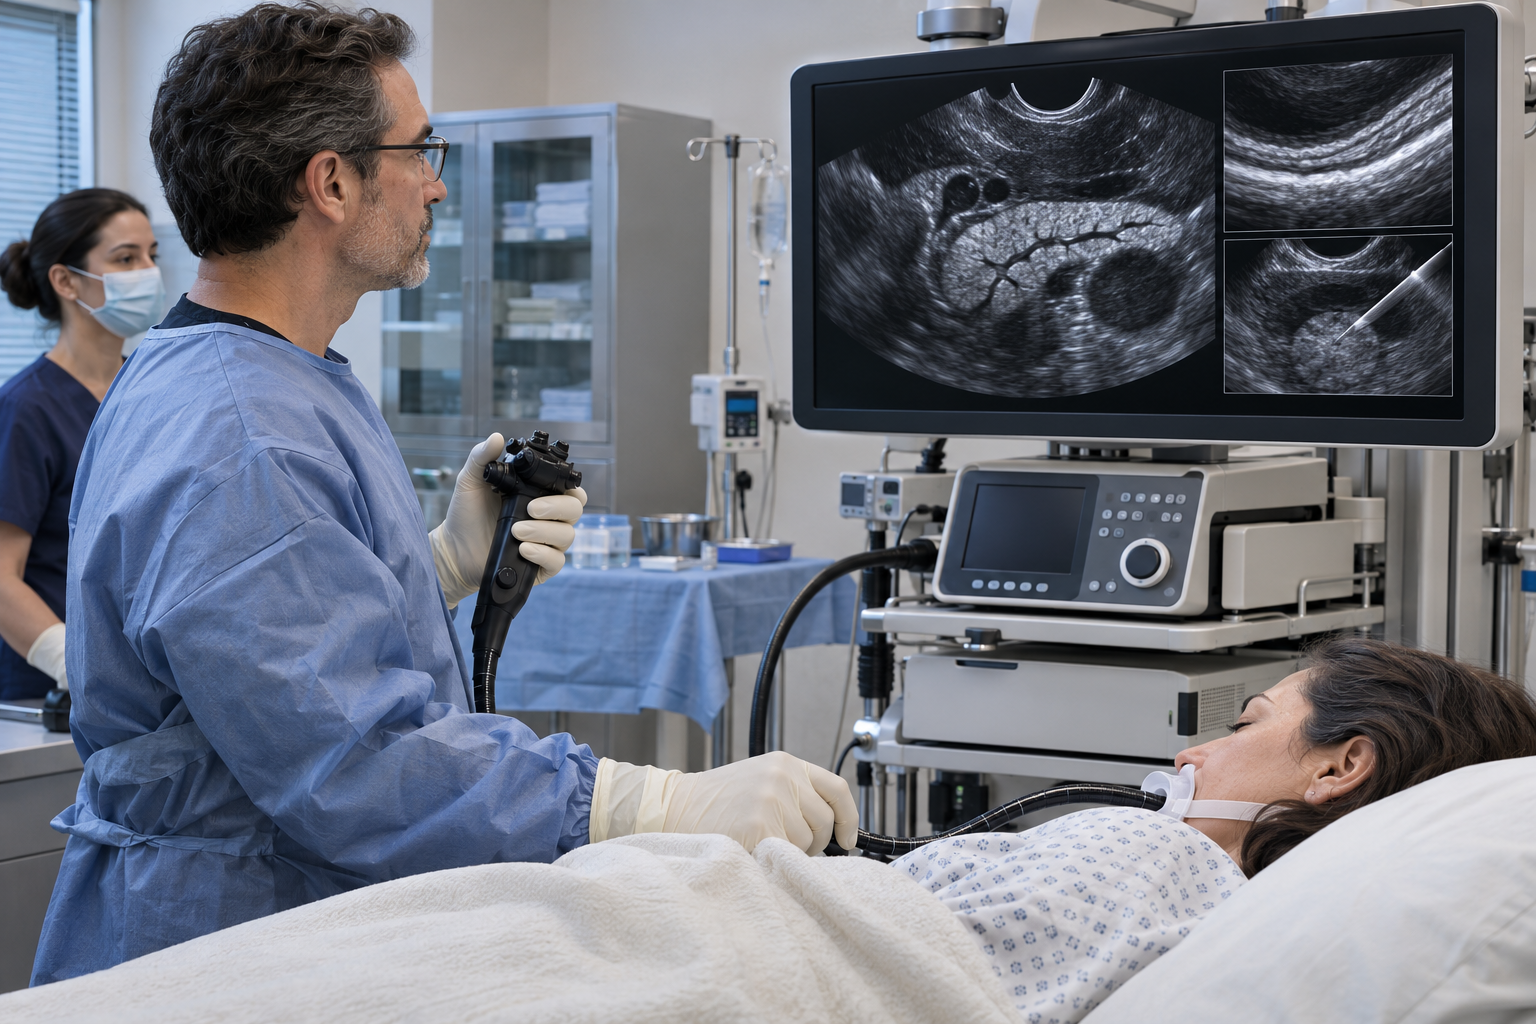
\includegraphics[width=\textwidth,keepaspectratio]{modalities/infographics/endoscopic_imaging_eus_realistic.png}
\end{center}
\begin{center}\footnotesize EUS places an ultrasound transducer close to the gastrointestinal wall and nearby organs, supporting detailed imaging and guided sampling. AI-generated illustration; ultrasound and biopsy panels are schematic.\end{center}

\section{Overview}
Endoscopic ultrasound (EUS), also known as endosonography, combines flexible endoscopy with high-frequency ultrasound imaging. An ultrasound transducer mounted at the tip of an endoscope visualizes the gastrointestinal wall and adjacent organs, blood vessels, lymph nodes and pathological structures.

Unlike conventional transabdominal ultrasound, EUS positions the transducer close to the target, reducing interference from abdominal fat, bowel gas and overlying anatomical structures. EUS is especially useful for pancreatic lesions, gastrointestinal subepithelial lesions, local staging of gastrointestinal malignancies, small biliary stones, image-guided tissue acquisition, lymph-node assessment and selected minimally invasive therapies.

\section{Where endoscopic ultrasound is used}

\subsection{Pancreatic diseases}
\begin{enumerate}[leftmargin=*,itemsep=0.45em,topsep=0.4em]
\item \textbf{Acinar cell carcinoma.} Useful imaging findings include: Solid heterogeneous pancreatic mass.
\item \textbf{Acute pancreatitis.} Useful imaging findings include: Variable, nonspecific parenchymal changes; EUS is generally supplementary and may investigate an occult biliary cause after the acute episode.
\item \textbf{Annular pancreas.} Useful imaging findings include: Pancreatic tissue surrounding the duodenum.
\item \textbf{Autoimmune pancreatitis.} Useful imaging findings include: Diffuse or focal hypoechoic pancreatic enlargement.
\item \textbf{Chronic pancreatitis.} Useful imaging findings include: Hyperechoic strands, lobularity, calcifications and ductal abnormalities.
\item \textbf{Early chronic pancreatitis.} Useful imaging findings include: Subtle, nonspecific parenchymal and ductal abnormalities; interpret with clinical findings and other imaging.
\item \textbf{Fatty pancreas.} Useful imaging findings include: Increased parenchymal echogenicity.
\item \textbf{Gastrinoma.} Useful imaging findings include: Hypoechoic neuroendocrine lesion.
\item \textbf{Glucagonoma.} Useful imaging findings include: Solid pancreatic mass with variable vascularity.
\item \textbf{Insulinoma.} Useful imaging findings include: Small, well-circumscribed hypoechoic lesion.
\item \textbf{Pancreas divisum.} Useful imaging findings include: Abnormal pancreatic ductal configuration.
\item \textbf{Pancreatic adenocarcinoma.} Useful imaging findings include: Irregular hypoechoic solid mass, sometimes with ductal obstruction.
\item \textbf{Pancreatic atrophy.} Useful imaging findings include: Reduced parenchymal volume.
\item \textbf{Pancreatic calcification.} Useful imaging findings include: Hyperechoic foci with acoustic shadowing.
\item \textbf{Pancreatic duct obstruction.} Useful imaging findings include: Upstream pancreatic duct dilatation.
\item \textbf{Pancreatic duct stone.} Useful imaging findings include: Echogenic intraductal focus with posterior shadowing.
\item \textbf{Pancreatic duct stricture.} Useful imaging findings include: Focal ductal narrowing with possible upstream dilatation.
\item \textbf{Pancreatic lipoma.} Useful imaging findings include: Well-defined hyperechoic lesion.
\item \textbf{Pancreatic lymphoma.} Useful imaging findings include: Hypoechoic pancreatic mass or diffuse enlargement.
\item \textbf{Pancreatic metastases.} Useful imaging findings include: Discrete solid lesions with variable echogenicity.
\item \textbf{Pancreatic necrosis.} Useful imaging findings include: Heterogeneous areas; nonenhancement is assessed with contrast-enhanced EUS, not conventional B-mode imaging.
\item \textbf{Pancreatic neuroendocrine tumor.} Useful imaging findings include: Well-defined, frequently hypoechoic and hypervascular mass.
\item \textbf{Solid pseudopapillary neoplasm.} Useful imaging findings include: Encapsulated mass with solid and cystic components.
\item \textbf{VIPoma.} Useful imaging findings include: Well-defined solid pancreatic lesion.
\end{enumerate}

\subsection{Pancreatic cystic lesions}
\begin{enumerate}[leftmargin=*,itemsep=0.45em,topsep=0.4em]
\item \textbf{Acute necrotic collection.} Useful imaging findings include: Heterogeneous fluid and necrotic material without a mature wall.
\item \textbf{Acute peripancreatic fluid collection.} Useful imaging findings include: Fluid collection without a mature encapsulating wall.
\item \textbf{Branch-duct IPMN.} Useful imaging findings include: Cystic lesion communicating with a pancreatic duct branch.
\item \textbf{Cystic degeneration of pancreatic carcinoma.} Useful imaging findings include: Irregular cystic mass with solid components.
\item \textbf{Cystic pancreatic neuroendocrine tumor.} Useful imaging findings include: Cystic lesion with an enhancing solid component.
\item \textbf{Main-duct IPMN.} Useful imaging findings include: Dilatation of the main pancreatic duct.
\item \textbf{Mixed-type IPMN.} Useful imaging findings include: Combined main-duct and branch-duct abnormalities.
\item \textbf{Mucinous cystic neoplasm.} Useful imaging findings include: Macrocystic lesion with septations and possible mural nodules.
\item \textbf{Pancreatic duplication cyst.} Useful imaging findings include: Cystic structure with characteristic layered wall.
\item \textbf{Pancreatic lymphangioma.} Useful imaging findings include: Multiloculated cystic lesion.
\item \textbf{Pancreatic lymphoepithelial cyst.} Useful imaging findings include: Cystic lesion with variable internal echogenicity.
\item \textbf{Pancreatic pseudocyst.} Useful imaging findings include: Fluid-filled collection with a defined wall.
\item \textbf{Pancreatic retention cyst.} Useful imaging findings include: Simple cystic lesion associated with ductal obstruction.
\item \textbf{Serous cystadenoma.} Useful imaging findings include: Microcystic or honeycomb-like architecture, sometimes with a central scar.
\item \textbf{Walled-off pancreatic necrosis.} Useful imaging findings include: Encapsulated collection containing heterogeneous necrotic debris.
\end{enumerate}
EUS morphology alone cannot reliably differentiate all pancreatic cystic neoplasms. Cyst-fluid analysis, cytology, molecular testing and MRI/MRCP may provide complementary information. EUS-guided sampling is selective and is most useful when the result is likely to change management.

\subsection{Gallbladder and biliary tract diseases}
\begin{enumerate}[leftmargin=*,itemsep=0.45em,topsep=0.4em]
\item \textbf{Acute cholecystitis.} Useful imaging findings include: Gallbladder wall thickening and surrounding inflammatory changes.
\item \textbf{Benign biliary stricture.} Useful imaging findings include: Relatively smooth focal bile duct narrowing.
\item \textbf{Biliary ascariasis.} Useful imaging findings include: Linear echogenic intraductal structure.
\item \textbf{Biliary microlithiasis.} Useful imaging findings include: Small echogenic intraductal structures.
\item \textbf{Biliary obstruction.} Useful imaging findings include: Proximal biliary dilatation and possible obstructing lesion.
\item \textbf{Biliary sludge.} Useful imaging findings include: Low-level intraluminal echoes, generally without shadowing.
\item \textbf{Choledochal cyst.} Useful imaging findings include: Abnormal cystic dilatation of the biliary tract.
\item \textbf{Choledocholithiasis.} Useful imaging findings include: Echogenic stone within the common bile duct.
\item \textbf{Cholelithiasis.} Useful imaging findings include: Hyperechoic gallstones with posterior acoustic shadowing.
\item \textbf{Cholesterol polyp.} Useful imaging findings include: Small echogenic polypoid lesion.
\item \textbf{Chronic cholecystitis.} Useful imaging findings include: Gallbladder wall thickening and possible calculi.
\item \textbf{Common bile duct dilatation.} Useful imaging findings include: Increased bile duct diameter.
\item \textbf{Distal cholangiocarcinoma.} Useful imaging findings include: Hypoechoic mass or irregular bile duct wall thickening.
\item \textbf{Gallbladder adenoma.} Useful imaging findings include: Solid polypoid lesion with variable echogenicity.
\item \textbf{Gallbladder adenomyomatosis.} Useful imaging findings include: Intramural cystic spaces and comet-tail artifacts.
\item \textbf{Gallbladder carcinoma.} Useful imaging findings include: Irregular wall thickening or infiltrative mass.
\item \textbf{Gallbladder microlithiasis.} Useful imaging findings include: Small echogenic particulate structures.
\item \textbf{Hilar cholangiocarcinoma.} Useful imaging findings include: Irregular hilar biliary lesion, when accessible.
\item \textbf{IgG4-related sclerosing cholangitis.} Useful imaging findings include: Possible bile duct wall thickening; EUS findings are nonspecific and do not establish the diagnosis.
\item \textbf{Malignant biliary stricture.} Useful imaging findings include: Irregular narrowing with abnormal surrounding tissue.
\item \textbf{Mirizzi syndrome.} Useful imaging findings include: Impacted gallstone associated with extrinsic biliary compression.
\item \textbf{Primary sclerosing cholangitis.} Useful imaging findings include: Possible ductal wall thickening; EUS findings are nonspecific and do not establish the diagnosis.
\end{enumerate}
EUS can assess accessible bile duct segments and investigate focal abnormalities, but it does not establish primary sclerosing or IgG4-related cholangitis. Diagnosis requires clinical and laboratory correlation with cholangiographic imaging, typically MRCP, and other testing as indicated.

\subsection{Ampullary and periampullary diseases}
\begin{enumerate}[leftmargin=*,itemsep=0.45em,topsep=0.4em]
\item \textbf{Ampullary adenoma.} Useful imaging findings include: Localized ampullary soft-tissue lesion.
\item \textbf{Ampullary carcinoma.} Useful imaging findings include: Irregular hypoechoic ampullary mass.
\item \textbf{Ampullary inflammatory enlargement.} Useful imaging findings include: Thickened or enlarged ampullary tissue.
\item \textbf{Ampullary neuroendocrine tumor.} Useful imaging findings include: Small solid hypoechoic lesion.
\item \textbf{Ampullary obstruction.} Useful imaging findings include: Ampullary abnormality with upstream ductal dilatation.
\item \textbf{Intraductal extension of ampullary tumor.} Useful imaging findings include: Extension of abnormal tissue into pancreatic or bile ducts.
\item \textbf{Periampullary carcinoma.} Useful imaging findings include: Mass involving the ampullary region or adjacent structures.
\item \textbf{Periampullary duodenal diverticulum.} Useful imaging findings include: Outpouching adjacent to the ampulla.
\end{enumerate}

\subsection{Esophageal diseases}
\begin{enumerate}[leftmargin=*,itemsep=0.45em,topsep=0.4em]
\item \textbf{Esophageal adenocarcinoma.} Useful imaging findings include: Irregular mural thickening with possible transmural invasion.
\item \textbf{Esophageal duplication cyst.} Useful imaging findings include: Anechoic or hypoechoic cystic lesion with a layered wall.
\item \textbf{Esophageal gastrointestinal stromal tumor.} Useful imaging findings include: Hypoechoic lesion commonly arising from muscularis propria.
\item \textbf{Esophageal granular cell tumor.} Useful imaging findings include: Small hypoechoic subepithelial lesion.
\item \textbf{Esophageal leiomyoma.} Useful imaging findings include: Well-defined hypoechoic lesion arising from a muscular layer.
\item \textbf{Esophageal lipoma.} Useful imaging findings include: Hyperechoic submucosal lesion.
\item \textbf{Esophageal lymphoma.} Useful imaging findings include: Abnormal wall thickening with possible lymphadenopathy.
\item \textbf{Esophageal schwannoma.} Useful imaging findings include: Solid hypoechoic subepithelial lesion.
\item \textbf{Esophageal squamous cell carcinoma.} Useful imaging findings include: Hypoechoic lesion disrupting normal esophageal wall layers.
\item \textbf{Esophageal varices.} Useful imaging findings include: Anechoic tubular vascular structures with Doppler flow.
\item \textbf{Esophageal wall infiltration.} Useful imaging findings include: Loss or disruption of normal wall architecture.
\item \textbf{Extrinsic esophageal compression.} Useful imaging findings include: External structure compressing an otherwise preserved esophageal wall.
\item \textbf{Paraesophageal varices.} Useful imaging findings include: Dilated vascular channels outside the esophageal wall.
\end{enumerate}

\subsection{Gastric diseases}
\begin{enumerate}[leftmargin=*,itemsep=0.45em,topsep=0.4em]
\item \textbf{Advanced gastric carcinoma.} Useful imaging findings include: Deep mural invasion and possible adjacent organ involvement.
\item \textbf{Early gastric carcinoma.} Useful imaging findings include: Localized superficial wall abnormality.
\item \textbf{Ectopic pancreas.} Useful imaging findings include: Heterogeneous subepithelial lesion, sometimes containing duct-like structures.
\item \textbf{Gastric adenocarcinoma.} Useful imaging findings include: Irregular hypoechoic wall thickening and layer disruption.
\item \textbf{Gastric amyloidosis.} Useful imaging findings include: Variable thickening of gastric wall layers.
\item \textbf{Gastric duplication cyst.} Useful imaging findings include: Cystic lesion with layered wall.
\item \textbf{Gastric extrinsic compression.} Useful imaging findings include: External mass compressing the gastric wall.
\item \textbf{Gastric gastrointestinal stromal tumor (GIST).} GIST is a mesenchymal tumor that often arises from the muscularis propria; EUS assesses layer of origin, margins, and risk features. Useful imaging findings include: Hypoechoic mass commonly arising from muscularis propria.
\item \textbf{Gastric glomus tumor.} Useful imaging findings include: Hypoechoic or heterogeneous vascular mass.
\item \textbf{Gastric inflammatory fibroid polyp.} Useful imaging findings include: Hypoechoic lesion involving mucosal or submucosal layers.
\item \textbf{Gastric leiomyoma.} Useful imaging findings include: Homogeneous hypoechoic muscular lesion.
\item \textbf{Gastric linitis plastica.} Useful imaging findings include: Diffuse infiltrative wall thickening and loss of normal stratification.
\item \textbf{Gastric lipoma.} Useful imaging findings include: Homogeneous hyperechoic submucosal lesion.
\item \textbf{Gastric lymphoma.} Useful imaging findings include: Diffuse or localized hypoechoic wall thickening.
\item \textbf{Gastric MALT lymphoma.} Useful imaging findings include: Variable mucosal and submucosal thickening.
\item \textbf{Gastric metastases.} Useful imaging findings include: Focal or diffuse mural infiltration.
\item \textbf{Gastric neuroendocrine tumor.} Useful imaging findings include: Small hypoechoic mucosal or submucosal lesion.
\item \textbf{Gastric schwannoma.} Useful imaging findings include: Well-defined hypoechoic subepithelial lesion.
\item \textbf{Gastric varices.} Useful imaging findings include: Tortuous anechoic vascular channels with Doppler flow.
\item \textbf{M\'en\'etrier disease.} Useful imaging findings include: Predominantly mucosal thickening.
\end{enumerate}

\subsection{Duodenal and small intestinal diseases}
\begin{enumerate}[leftmargin=*,itemsep=0.45em,topsep=0.4em]
\item \textbf{Brunner gland hamartoma.} Useful imaging findings include: Variable heterogeneous or cystic submucosal lesion.
\item \textbf{Duodenal adenocarcinoma.} Useful imaging findings include: Irregular hypoechoic mural lesion.
\item \textbf{Duodenal duplication cyst.} Useful imaging findings include: Cystic lesion with layered wall.
\item \textbf{Duodenal endometriosis.} Useful imaging findings include: Hypoechoic infiltrative mural lesion in selected cases.
\item \textbf{Duodenal GIST.} Useful imaging findings include: Solid hypoechoic lesion arising from muscularis propria.
\item \textbf{Duodenal lipoma.} Useful imaging findings include: Hyperechoic submucosal mass.
\item \textbf{Duodenal lymphoma.} Useful imaging findings include: Abnormal mural thickening.
\item \textbf{Duodenal neuroendocrine tumor.} Useful imaging findings include: Small hypoechoic subepithelial lesion.
\item \textbf{Duodenal wall invasion by pancreatic carcinoma.} Useful imaging findings include: Disruption of wall layers by an adjacent mass.
\item \textbf{Small intestinal subepithelial lesion.} Useful imaging findings include: Lesion characterized by wall-layer origin and echogenicity.
\end{enumerate}
Conventional EUS principally accesses the upper gastrointestinal tract and selected lower regions. Most of the jejunum and ileum cannot be routinely reached.

\subsection{Colorectal and anorectal diseases}
\begin{enumerate}[leftmargin=*,itemsep=0.45em,topsep=0.4em]
\item \textbf{Anal carcinoma.} Useful imaging findings include: Irregular infiltrative hypoechoic lesion.
\item \textbf{Anal sphincter atrophy.} Useful imaging findings include: Reduced muscle thickness.
\item \textbf{Anal sphincter injury.} Useful imaging findings include: Discontinuity of sphincter musculature.
\item \textbf{Early rectal carcinoma.} Useful imaging findings include: Localized superficial tumor infiltration.
\item \textbf{Intersphincteric abscess.} Useful imaging findings include: Collection between internal and external sphincters.
\item \textbf{Locally advanced rectal carcinoma.} Useful imaging findings include: Extension beyond muscularis propria.
\item \textbf{Perianal abscess.} Useful imaging findings include: Hypoechoic or heterogeneous fluid collection.
\item \textbf{Perianal fistula.} Useful imaging findings include: Hypoechoic fistulous tract.
\item \textbf{Perirectal lymphadenopathy.} Useful imaging findings include: Enlarged lymph nodes adjacent to the rectum.
\item \textbf{Rectal adenocarcinoma.} Useful imaging findings include: Hypoechoic mural mass disrupting normal wall layers.
\item \textbf{Rectal duplication cyst.} Useful imaging findings include: Cystic lesion adjacent to or within the rectal wall.
\item \textbf{Rectal endometriosis.} Useful imaging findings include: Hypoechoic infiltrative lesion frequently involving muscularis propria.
\item \textbf{Rectal GIST.} Useful imaging findings include: Hypoechoic muscularis propria lesion.
\item \textbf{Rectal leiomyoma.} Useful imaging findings include: Homogeneous hypoechoic muscular lesion.
\item \textbf{Rectal lipoma.} Useful imaging findings include: Hyperechoic submucosal lesion.
\item \textbf{Rectal lymphoma.} Useful imaging findings include: Abnormal mural thickening.
\item \textbf{Rectal neuroendocrine tumor.} Useful imaging findings include: Small hypoechoic submucosal lesion.
\item \textbf{Rectal varices.} Useful imaging findings include: Dilated submucosal vascular channels.
\end{enumerate}
Some of these conditions are evaluated using dedicated endorectal ultrasound (ERUS) or endoanal ultrasound (EAUS), rather than a conventional gastrointestinal echoendoscope.

\subsection{Hepatic diseases}
\begin{enumerate}[leftmargin=*,itemsep=0.45em,topsep=0.4em]
\item \textbf{Focal nodular hyperplasia.} Useful imaging findings include: Solid lesion with variable echogenicity.
\item \textbf{Granulomatous liver disease.} Useful imaging findings include: Variable focal or diffuse abnormalities.
\item \textbf{Hepatic abscess.} Useful imaging findings include: Complex fluid collection with internal echoes.
\item \textbf{Hepatic adenoma.} Useful imaging findings include: Solid lesion with variable internal architecture.
\item \textbf{Hepatic hemangioma.} Useful imaging findings include: Frequently well-defined hyperechoic lesion.
\item \textbf{Hepatic lymphoma.} Useful imaging findings include: Hypoechoic focal lesions or infiltrative abnormalities.
\item \textbf{Hepatic metastases.} Useful imaging findings include: Focal lesions with variable echogenicity.
\item \textbf{Hepatic steatosis.} Useful imaging findings include: Increased hepatic echogenicity.
\item \textbf{Hepatocellular carcinoma.} Useful imaging findings include: Focal solid lesion with variable vascular enhancement.
\item \textbf{Intrahepatic cholangiocarcinoma.} Useful imaging findings include: Irregular hypoechoic hepatic mass.
\item \textbf{Liver cirrhosis.} Useful imaging findings include: Coarse echotexture and irregular surface where visible.
\item \textbf{Simple hepatic cyst.} Useful imaging findings include: Anechoic lesion with posterior acoustic enhancement.
\end{enumerate}
EUS visualizes selected hepatic segments, particularly portions of the left lobe. It does not replace comprehensive liver imaging with transabdominal ultrasound, CT or MRI.

\subsection{Lymphatic and lymph node diseases}
\begin{enumerate}[leftmargin=*,itemsep=0.45em,topsep=0.4em]
\item \textbf{Celiac lymphadenopathy.} Useful imaging findings include: Enlarged lymph nodes around celiac vessels.
\item \textbf{Hodgkin lymphoma.} Useful imaging findings include: Enlarged hypoechoic lymph nodes.
\item \textbf{Mediastinal lymphadenopathy.} Useful imaging findings include: Enlarged nodes accessible through the esophageal wall.
\item \textbf{Metastatic lymphadenopathy.} Useful imaging findings include: Rounded hypoechoic nodes with possible sharp margins.
\item \textbf{Necrotic lymphadenopathy.} Useful imaging findings include: Heterogeneous nodes containing hypoechoic or cystic regions.
\item \textbf{Non-Hodgkin lymphoma.} Useful imaging findings include: Multiple enlarged or conglomerate lymph nodes.
\item \textbf{Peripancreatic lymphadenopathy.} Useful imaging findings include: Enlarged nodes adjacent to the pancreas.
\item \textbf{Periportal lymphadenopathy.} Useful imaging findings include: Enlarged nodes around portal structures.
\item \textbf{Reactive lymphadenopathy.} Useful imaging findings include: Variable nodal enlargement, sometimes with preserved architecture.
\item \textbf{Retroperitoneal lymphadenopathy.} Useful imaging findings include: Enlarged nodes within accessible retroperitoneal regions.
\item \textbf{Sarcoidosis.} Useful imaging findings include: Multiple enlarged mediastinal or abdominal lymph nodes.
\item \textbf{Tuberculous lymphadenitis.} Useful imaging findings include: Enlarged nodes with possible necrosis.
\end{enumerate}
Lymph-node morphology alone cannot reliably distinguish infection, inflammation and malignancy. EUS-guided tissue acquisition can improve diagnostic specificity.

\subsection{Mediastinal and thoracic diseases}
\begin{enumerate}[leftmargin=*,itemsep=0.45em,topsep=0.4em]
\item \textbf{Bronchogenic cyst.} Useful imaging findings include: Well-defined cystic mediastinal lesion.
\item \textbf{Centrally located lung carcinoma.} Useful imaging findings include: Solid pulmonary lesion adjacent to the esophagus.
\item \textbf{Mediastinal duplication cyst.} Useful imaging findings include: Cystic lesion with characteristic wall architecture.
\item \textbf{Mediastinal lymphoma.} Useful imaging findings include: Enlarged hypoechoic lymph nodes or confluent mass.
\item \textbf{Mediastinal metastases.} Useful imaging findings include: Solid masses or abnormal lymph nodes.
\item \textbf{Mediastinal sarcoidosis.} Useful imaging findings include: Multiple enlarged lymph nodes.
\item \textbf{Mediastinal schwannoma.} Useful imaging findings include: Well-defined hypoechoic solid mass.
\item \textbf{Mediastinal tuberculosis.} Useful imaging findings include: Lymphadenopathy with variable necrotic components.
\item \textbf{Pleural effusion.} Useful imaging findings include: Anechoic fluid within the pleural space.
\item \textbf{Posterior mediastinal tumor.} Useful imaging findings include: Solid lesion adjacent to the esophagus.
\end{enumerate}
Endobronchial ultrasound (EBUS) is related but distinct; it accesses tracheobronchial and mediastinal structures through the respiratory tract.

\subsection{Adrenal and retroperitoneal diseases}
\begin{enumerate}[leftmargin=*,itemsep=0.45em,topsep=0.4em]
\item \textbf{Adrenal adenoma.} Useful imaging findings include: Discrete adrenal lesion with variable echogenicity.
\item \textbf{Adrenal cyst.} Useful imaging findings include: Anechoic adrenal lesion.
\item \textbf{Adrenal hemorrhage.} Useful imaging findings include: Heterogeneous adrenal enlargement.
\item \textbf{Adrenal metastasis.} Useful imaging findings include: Enlarged or irregular adrenal mass.
\item \textbf{Adrenal myelolipoma.} Useful imaging findings include: Frequently echogenic heterogeneous lesion.
\item \textbf{Adrenocortical carcinoma.} Useful imaging findings include: Large heterogeneous adrenal lesion.
\item \textbf{Pheochromocytoma.} Useful imaging findings include: Solid adrenal lesion with variable vascularity.
\item \textbf{Retroperitoneal cyst.} Useful imaging findings include: Cystic lesion adjacent to accessible gastrointestinal structures.
\item \textbf{Retroperitoneal lymphoma.} Useful imaging findings include: Hypoechoic masses or enlarged lymph nodes.
\item \textbf{Retroperitoneal sarcoma.} Useful imaging findings include: Large heterogeneous soft-tissue mass.
\end{enumerate}
The left adrenal gland is generally more accessible than the right. Suspected pheochromocytoma should be investigated biochemically before invasive tissue sampling is considered.

\subsection{Vascular diseases and abnormalities}
\begin{enumerate}[leftmargin=*,itemsep=0.45em,topsep=0.4em]
\item \textbf{Esophageal varices.} Useful imaging findings include: Dilated submucosal venous structures.
\item \textbf{Gastric varices.} Useful imaging findings include: Dilated vascular channels within or around the gastric wall.
\item \textbf{Pancreatic tumor vascular invasion.} Useful imaging findings include: Abnormal tumor-vessel interface, encasement or luminal distortion.
\item \textbf{Perigastric collateral circulation.} Useful imaging findings include: Multiple abnormal venous channels.
\item \textbf{Portal cavernous transformation.} Useful imaging findings include: Multiple collateral vascular channels.
\item \textbf{Portal hypertension.} Useful imaging findings include: Dilated portosystemic collateral vessels.
\item \textbf{Portal vein thrombosis.} Useful imaging findings include: Intraluminal material and reduced or absent Doppler flow.
\item \textbf{Splenic artery aneurysm.} Useful imaging findings include: Focal arterial dilatation with Doppler flow.
\item \textbf{Splenic vein thrombosis.} Useful imaging findings include: Abnormal intraluminal echoes and impaired venous flow.
\item \textbf{Superior mesenteric vein thrombosis.} Useful imaging findings include: Venous filling abnormality and reduced flow.
\item \textbf{Tumor thrombus.} Useful imaging findings include: Intravascular tissue with possible internal vascularity.
\item \textbf{Visceral artery pseudoaneurysm.} Useful imaging findings include: Vascular sac with characteristic Doppler flow.
\end{enumerate}

\subsection{Other abdominal and extraluminal conditions}
\begin{enumerate}[leftmargin=*,itemsep=0.45em,topsep=0.4em]
\item \textbf{Abdominal duplication cyst.} Useful imaging findings include: Cystic lesion with characteristic wall layering.
\item \textbf{Ascites.} Useful imaging findings include: Anechoic fluid surrounding abdominal structures.
\item \textbf{Extraluminal gastrointestinal tumor.} Useful imaging findings include: Solid mass adjacent to the gastrointestinal tract.
\item \textbf{Intra-abdominal abscess.} Useful imaging findings include: Complex fluid-containing lesion.
\item \textbf{Intra-abdominal hematoma.} Useful imaging findings include: Heterogeneous collection with evolving echogenicity.
\item \textbf{Lymphocele.} Useful imaging findings include: Localized cystic fluid collection.
\item \textbf{Malignant ascites.} Useful imaging findings include: Fluid with possible associated peritoneal nodules.
\item \textbf{Omental metastases.} Useful imaging findings include: Abnormal nodular soft-tissue deposits.
\item \textbf{Peritoneal carcinomatosis.} Useful imaging findings include: Irregular peritoneal nodules or thickening.
\item \textbf{Postoperative pancreatic fluid collection.} Useful imaging findings include: Localized fluid collection near pancreatic structures.
\end{enumerate}



\subsection{Summary of catalogue}
\begin{tabular}{@{}p{0.70\textwidth}r@{}}
\toprule
\textbf{Disease category} & \textbf{Entries} \\
\midrule
Adrenal and retroperitoneal diseases & 10 \\
Ampullary and periampullary diseases & 8 \\
Colorectal and anorectal diseases & 18 \\
Duodenal and small intestinal diseases & 10 \\
Esophageal diseases & 13 \\
Gallbladder and biliary tract diseases & 22 \\
Gastric diseases & 20 \\
Hepatic diseases & 12 \\
Lymphatic and lymph node diseases & 12 \\
Mediastinal and thoracic diseases & 10 \\
Other abdominal and extraluminal conditions & 10 \\
Pancreatic cystic lesions & 15 \\
Pancreatic diseases & 24 \\
Total & 196 \\
Vascular diseases and abnormalities & 12 \\
\bottomrule
\end{tabular}

\subsection{Types of endoscopic ultrasound}
\begin{longtable}{@{}p{0.38\textwidth}p{0.56\textwidth}@{}}
\toprule
\textbf{EUS technique} & \textbf{Primary application} \\
\midrule
\endfirsthead
\toprule
\textbf{EUS technique} & \textbf{Primary application} \\
\midrule
\endhead
B-mode EUS & Grayscale structural imaging \\
Color Doppler EUS & Blood flow visualization \\
Contrast-enhanced EUS & Tissue vascularity and perfusion assessment \\
Contrast-enhanced harmonic EUS & Microvascular enhancement characterization \\
Endoanal ultrasound (EAUS) & Anal sphincter and perianal anatomy \\
Endorectal ultrasound (ERUS) & Rectal wall and surrounding tissue evaluation \\
EUS shear-wave elastography & Quantitative tissue stiffness estimation \\
EUS strain elastography & Relative tissue stiffness assessment \\
High-frequency miniprobe EUS & Superficial gastrointestinal wall characterization \\
Intraductal ultrasound (IDUS) & High-resolution pancreatic and biliary duct imaging \\
Linear-array EUS & Anatomical imaging and image-guided interventions \\
Power Doppler EUS & Detection of low-velocity blood flow \\
Radial EUS & Circumferential cross-sectional anatomical imaging \\
Spectral Doppler EUS & Quantitative blood flow assessment \\
Three-dimensional EUS & Volumetric reconstruction \\
\bottomrule
\end{longtable}

\subsection{Normal gastrointestinal wall architecture}
One distinctive capability of EUS is visualization of the individual sonographic layers of the gastrointestinal wall.

\begin{longtable}{@{}p{0.15\textwidth}p{0.24\textwidth}p{0.55\textwidth}@{}}
\toprule
\textbf{Layer} & \textbf{Echogenicity} & \textbf{Corresponding anatomical structure} \\
\midrule
\endfirsthead
\toprule
\textbf{Layer} & \textbf{Echogenicity} & \textbf{Corresponding anatomical structure} \\
\midrule
\endhead
Layer 1 & Hyperechoic & Superficial mucosa and luminal interface \\
Layer 2 & Hypoechoic & Deep mucosa \\
Layer 3 & Hyperechoic & Submucosa \\
Layer 4 & Hypoechoic & Muscularis propria \\
Layer 5 & Hyperechoic & Serosa, adventitia and surrounding interface \\
\bottomrule
\end{longtable}
These are the conventional five sonographic layers. Higher-frequency imaging may resolve additional layers.

\subsection{Differentiation of subepithelial lesions}
\begin{longtable}{@{}p{0.28\textwidth}p{0.27\textwidth}p{0.39\textwidth}@{}}
\toprule
\textbf{Lesion} & \textbf{Typical layer of origin} & \textbf{Echogenicity} \\
\midrule
\endfirsthead
\toprule
Duplication cyst & Variable & Anechoic or hypoechoic \\
\midrule
\endhead
Ectopic pancreas & Variable, often third or fourth layer & Heterogeneous \\
GIST & Usually fourth layer & Hypoechoic \\
Granular cell tumor & Second or third layer & Hypoechoic \\
Leiomyoma & Second or fourth layer & Hypoechoic \\
\textbf{Lesion} & \textbf{Typical layer of origin} & \textbf{Echogenicity} \\
Lipoma & Third layer & Hyperechoic \\
Neuroendocrine tumor & Second or third layer & Hypoechoic \\
Schwannoma & Usually fourth layer & Hypoechoic \\
Varices & Third layer or extramural & Anechoic with Doppler flow \\
\bottomrule
\end{longtable}

\subsection{Contrast-enhanced EUS}
Contrast-enhanced EUS uses intravenously administered microbubble contrast agents to characterize tissue perfusion and microvascular architecture.

\begin{longtable}{@{}p{0.40\textwidth}p{0.54\textwidth}@{}}
\toprule
\textbf{Disease or condition} & \textbf{Typical enhancement pattern} \\
\midrule
\endfirsthead
\toprule
\textbf{Disease or condition} & \textbf{Typical enhancement pattern} \\
\midrule
\endhead
Autoimmune pancreatitis & Variable homogeneous enhancement \\
Chronic inflammatory pancreatic mass & Variable, sometimes isoenhancement \\
Gallbladder carcinoma & Irregular or heterogeneous vascular enhancement \\
Gallbladder sludge & Absent enhancement \\
GIST & Variable enhancement, sometimes with irregular intratumoral vessels \\
Intracystic mucus or debris & Generally absent internal enhancement \\
Necrotic lymph node & Nonenhancing central region \\
Pancreatic cyst mural nodule & Enhancement of viable nodular tissue \\
Pancreatic ductal adenocarcinoma & Hypoenhancement relative to surrounding pancreas \\
Pancreatic necrosis & Absent enhancement in necrotic tissue \\
Pancreatic neuroendocrine tumor & Frequently hyperenhancement \\
Pancreatic pseudocyst & No enhancement of internal fluid \\
\bottomrule
\end{longtable}
Enhancement patterns overlap among diseases and should not be treated as definitive histological classifications.

\subsection{EUS elastography}
EUS elastography estimates tissue mechanical properties. Diseased tissues may differ in stiffness because of fibrosis, inflammation, cellular proliferation or extracellular matrix changes.

\begin{longtable}{@{}p{0.40\textwidth}p{0.54\textwidth}@{}}
\toprule
\textbf{Disease or condition} & \textbf{Typical elastographic finding} \\
\midrule
\endfirsthead
\toprule
\textbf{Disease or condition} & \textbf{Typical elastographic finding} \\
\midrule
\endhead
Autoimmune pancreatitis & Increased or heterogeneous stiffness \\
Chronic pancreatitis & Increased stiffness associated with fibrosis \\
Hepatic fibrosis & Increased hepatic stiffness \\
Malignant lymphadenopathy & Frequently increased stiffness \\
Pancreatic adenocarcinoma & Frequently increased stiffness \\
Pancreatic fibrosis & Increased parenchymal stiffness \\
Pancreatic neuroendocrine tumor & Variable stiffness \\
Reactive lymphadenopathy & Variable, often relatively softer tissue \\
\bottomrule
\end{longtable}
Elastography is supplementary and cannot reliably distinguish malignancy from inflammation in every case.

\subsection{EUS-guided diagnostic and therapeutic procedures}
\begin{longtable}{@{}p{0.48\textwidth}p{0.46\textwidth}@{}}
\toprule
\textbf{Procedure} & \textbf{Clinical application} \\
\midrule
\endfirsthead
\toprule
\textbf{Procedure} & \textbf{Clinical application} \\
\midrule
\endhead
EUS-guided adrenal biopsy & Selected adrenal mass characterization \\
EUS-guided biliary drainage & Management of biliary obstruction \\
EUS-guided celiac plexus block & Selected pancreatic pain management \\
EUS-guided celiac plexus neurolysis & Selected pancreatic cancer pain management \\
EUS-guided choledochoduodenostomy & Creation of a bile duct drainage pathway \\
EUS-guided cyst ablation & Specialized or investigational pancreatic cyst treatment \\
EUS-guided fiducial placement & Radiation therapy targeting \\
EUS-guided fine-needle aspiration (FNA) & Cytological sampling \\
EUS-guided fine-needle biopsy (FNB) & Histological tissue acquisition \\
EUS-guided gallbladder drainage & Management of selected high-risk cholecystitis patients \\
EUS-guided gastroenterostomy & Selected gastric outlet obstruction \\
EUS-guided glue injection & Selected gastric variceal obliteration \\
EUS-guided hepaticogastrostomy & Drainage of intrahepatic bile ducts \\
EUS-guided liver biopsy & Selected hepatic tissue sampling \\
EUS-guided lymph node biopsy & Investigation of lymphadenopathy \\
EUS-guided pancreatic cyst aspiration & Selected cyst-fluid analysis when results are likely to change management \\
EUS-guided pancreatic duct drainage & Selected pancreatic duct obstruction \\
EUS-guided pelvic abscess drainage & Selected accessible pelvic collections \\
EUS-guided portal pressure measurement & Emerging portal hypertension assessment \\
EUS-guided pseudocyst drainage & Drainage of symptomatic pancreatic pseudocysts \\
EUS-guided radiofrequency ablation & Selected pancreatic lesions; specialized or emerging \\
EUS-guided tumor injection & Investigational localized therapies \\
EUS-guided vascular coil embolization & Selected gastric varices \\
EUS-guided walled-off necrosis drainage & Management of selected pancreatic necrotic collections \\
\bottomrule
\end{longtable}

\subsection{Physical characteristics of EUS}
\begin{longtable}{@{}p{0.39\textwidth}p{0.55\textwidth}@{}}
\toprule
\textbf{Parameter} & \textbf{Typical characteristics} \\
\midrule
\endfirsthead
\toprule
\textbf{Parameter} & \textbf{Typical characteristics} \\
\midrule
\endhead
Contrast mechanism & Acoustic impedance differences \\
Conventional operating frequency & Approximately 5--12 MHz \\
Functional imaging & Doppler and contrast enhancement \\
High-frequency miniprobe & Approximately 12--30 MHz \\
Imaging dimensions & Two-dimensional, dynamic and selected three-dimensional acquisitions \\
Invasiveness & Minimally invasive endoscopic examination \\
Ionizing radiation & None \\
Mechanical characterization & Elastography \\
Penetration depth & Frequency- and tissue-dependent \\
Physical mechanism & Acoustic pulse--echo imaging \\
Spatial resolution & Submillimeter under favorable conditions \\
Tissue acquisition & FNA and FNB \\
Transducer position & Inside gastrointestinal lumen \\
\bottomrule
\end{longtable}

Acoustic wavelength is given by:
\[
\lambda=\frac{c}{f}
\]
where $c$ is the speed of sound in tissue and $f$ is ultrasound frequency. Assuming a soft-tissue sound velocity of approximately 1,540 m/s:

\begin{longtable}{@{}p{0.45\textwidth}p{0.49\textwidth}@{}}
\toprule
\textbf{Transducer frequency} & \textbf{Acoustic wavelength} \\
\midrule
\endfirsthead
\toprule
5 MHz & 308 $\mu$m \\
\midrule
\endhead
7.5 MHz & 205 $\mu$m \\
10 MHz & 154 $\mu$m \\
12 MHz & 128 $\mu$m \\
20 MHz & 77 $\mu$m \\
30 MHz & 51 $\mu$m \\
\textbf{Transducer frequency} & \textbf{Acoustic wavelength} \\
\bottomrule
\end{longtable}
Acoustic wavelength is not the same as image resolution, which also depends on pulse length, beam width, focusing and signal processing.

\subsection{Quantitative EUS parameters}
\begin{longtable}{@{}p{0.38\textwidth}p{0.56\textwidth}@{}}
\toprule
\textbf{Parameter} & \textbf{Clinical or research significance} \\
\midrule
\endfirsthead
\toprule
\textbf{Parameter} & \textbf{Clinical or research significance} \\
\midrule
\endhead
Common bile duct diameter & Biliary obstruction assessment \\
Cyst wall thickness & Cystic lesion characterization \\
Elastic modulus & Estimated tissue stiffness \\
Gastrointestinal wall thickness & Inflammation or infiltration \\
Layer-specific thickness & Depth of pathological involvement \\
Lesion cross-sectional area & Morphological assessment \\
Lesion diameter & Tumor or cyst dimensions \\
Lesion volume & Tumor or cyst burden \\
Lymph node short-axis diameter & Lymphadenopathy assessment \\
Mean flow velocity & Hemodynamic assessment \\
Mural nodule diameter & Pancreatic cyst risk assessment \\
Pancreatic duct diameter & Ductal obstruction and structural abnormalities \\
Peak contrast enhancement & Relative tissue perfusion \\
Peak systolic velocity & Arterial flow \\
Resistive index & Vascular resistance estimation \\
Septal thickness & Internal cyst architecture \\
Shear-wave velocity & Tissue mechanical properties \\
Strain ratio & Relative tissue deformation \\
Time to peak enhancement & Contrast perfusion dynamics \\
Wash-in rate & Microvascular perfusion \\
Washout rate & Contrast clearance dynamics \\
\bottomrule
\end{longtable}

\subsection{Standardized diagnostic and classification systems}
\begin{longtable}{@{}p{0.38\textwidth}p{0.56\textwidth}@{}}
\toprule
\textbf{Classification system} & \textbf{Primary application} \\
\midrule
\endfirsthead
\toprule
\textbf{Classification system} & \textbf{Primary application} \\
\midrule
\endhead
AJCC staging & Anatomical cancer staging \\
ASGE recommendations & Endoscopic and EUS clinical practice \\
Conventional EUS criteria & Chronic pancreatitis assessment \\
ESGE recommendations & EUS diagnostic and therapeutic procedures \\
Forrest classification & Peptic ulcer bleeding, primarily endoscopic \\
GIST risk classification & Tumor recurrence risk incorporating histopathology \\
Kyoto guidelines & IPMN risk assessment and management \\
Paris classification & Superficial gastrointestinal neoplastic lesions \\
Parks classification & Anal fistula anatomy \\
Revised Atlanta classification & Pancreatitis and pancreatic fluid collections \\
Rosemont classification & EUS features of chronic pancreatitis \\
TNM staging & Gastrointestinal and pancreatic malignancies \\
\bottomrule
\end{longtable}

\subsection{Comparison with other diagnostic modalities}
\begin{longtable}{@{}p{0.25\textwidth}p{0.16\textwidth}p{0.16\textwidth}p{0.16\textwidth}p{0.19\textwidth}@{}}
\toprule
\textbf{Feature} & \textbf{EUS} & \textbf{Abdominal ultrasound} & \textbf{CT} & \textbf{MRI/MRCP} \\
\midrule
\endfirsthead
\toprule
\textbf{Feature} & \textbf{EUS} & \textbf{Abdominal ultrasound} & \textbf{CT} & \textbf{MRI/MRCP} \\
\midrule
\endhead
Direct tissue acquisition & Yes & Yes, percutaneously & Yes, percutaneously & Specialized \\
Distant metastasis staging & Limited & Limited & Excellent & Excellent for selected organs \\
Gastrointestinal wall-layer visualization & Excellent & Limited & Limited & Selected applications \\
Ionizing radiation & No & No & Yes & No \\
Operator dependence & High & High & Relatively low & Relatively low \\
Pancreatic cyst characterization & Excellent & Variable & Good & Excellent \\
Physical mechanism & Ultrasound & Ultrasound & X-rays & Magnetic resonance \\
Real-time imaging & Yes & Yes & Specialized & Specialized \\
Sedation requirement & Frequently & No & Usually no & Usually no \\
Small biliary stone detection & Excellent & Variable & Limited & Good to excellent \\
Small pancreatic lesion detection & Excellent & Variable & Good & Good to excellent \\
Therapeutic interventions & Extensive & Selected & Selected & Specialized \\
Transducer location & Internal & External & Not applicable & Not applicable \\
Whole abdominal coverage & Limited & Good & Excellent & Excellent \\
\bottomrule
\end{longtable}

\subsection{Published resources for EUS imaging}
\begin{longtable}{@{}p{0.48\textwidth}p{0.46\textwidth}@{}}
\toprule
\textbf{Resource} & \textbf{Primary utility} \\
\midrule
\endfirsthead
\toprule
\textbf{Resource} & \textbf{Primary utility} \\
\midrule
\endhead
American Society for Gastrointestinal Endoscopy & EUS clinical guidelines and educational resources \\
Endoscopy International Open & Clinical studies and endoscopic images \\
European Society of Gastrointestinal Endoscopy & Diagnostic and therapeutic EUS guidelines \\
Grand Challenge & Medical imaging and computer vision datasets \\
PubMed Central & Published EUS images and open-access research \\
Radiopaedia & Complementary radiological findings \\
VideoGIE & Published endoscopic and EUS procedural videos \\
Zenodo & Research datasets and supplementary imaging materials \\
\bottomrule
\end{longtable}
Publicly accessible, comprehensively annotated EUS datasets are less common than CT, MRI, conventional ultrasound and optical endoscopy datasets.

\subsection{Recommended metadata for an EUS dataset}
\begin{longtable}{@{}p{0.45\textwidth}p{0.49\textwidth}@{}}
\toprule
\textbf{Attribute} & \textbf{Example} \\
\midrule
Acquisition format & Static image and dynamic video \\
Acquisition location & Duodenum \\
Acquisition mode & B-mode \\
Anatomical region & Pancreatic head \\
Contrast enhancement & Hypoenhancement \\
Diagnostic reference standard & Histopathological confirmation \\
Disease & Pancreatic ductal adenocarcinoma \\
EUS subtype & Linear-array EUS \\
Image annotation & Tumor segmentation mask \\
Image format & DICOM, PNG or MP4 \\
Image license & Specified license \\
Imaging modality & Endoscopic ultrasound \\
Lesion dimensions & 24 $\times$ 18 mm \\
Lesion echogenicity & Hypoechoic \\
Lesion echotexture & Heterogeneous \\
Lesion margins & Irregular \\
Pancreatic duct diameter & 5 mm \\
Publication reference & DOI or PMID \\
Supplementary mode & Contrast-enhanced harmonic EUS \\
Tissue acquisition & EUS-guided FNB \\
Transducer frequency & 10 MHz \\
Vascular involvement & Recorded \\
\bottomrule
\end{longtable}
The example values are illustrative.

\subsection{Artificial intelligence applications in EUS}
\begin{longtable}{@{}p{0.47\textwidth}p{0.47\textwidth}@{}}
\toprule
\textbf{AI application} & \textbf{Computational task} \\
\midrule
\endfirsthead
\toprule
\textbf{AI application} & \textbf{Computational task} \\
\midrule
\endhead
Anatomical landmark recognition & Object detection \\
Automated EUS reporting & Multimodal language modeling \\
Automated lesion measurement & Geometric image analysis \\
Biliary stone detection & Object detection \\
Biopsy needle tracking & Temporal object tracking \\
Chronic pancreatitis assessment & Feature extraction and classification \\
Contrast enhancement analysis & Temporal signal processing \\
Elastographic tissue characterization & Quantitative image analysis \\
EUS video quality assessment & Quality classification \\
Gastrointestinal wall-layer segmentation & Multiclass segmentation \\
Lymph node characterization & Classification \\
Pancreatic cancer detection & Image classification and object detection \\
Pancreatic cyst classification & Multiclass classification \\
Pancreatic duct segmentation & Semantic segmentation \\
Pancreatic tumor segmentation & Semantic segmentation \\
Subepithelial lesion characterization & Classification \\
Tumor invasion assessment & Spatial relationship analysis \\
Vascular structure identification & Segmentation \\
\bottomrule
\end{longtable}

\subsection{Clinical importance of EUS}
\begin{longtable}{@{}p{0.55\textwidth}p{0.39\textwidth}@{}}
\toprule
\textbf{Clinical application} & \textbf{Clinical status} \\
\midrule
\endfirsthead
\toprule
\textbf{Clinical application} & \textbf{Clinical status} \\
\midrule
\endhead
Autonomous AI-based EUS diagnosis & Investigational \\
Contrast-enhanced EUS & Specialized supplementary application \\
Detection of small common bile duct stones & Established \\
Detection of small pancreatic tumors & Established \\
Direct portal pressure measurement & Emerging \\
EUS elastography & Supplementary application \\
EUS-guided biliary drainage & Specialized clinical application \\
EUS-guided gallbladder drainage & Specialized clinical application \\
EUS-guided tumor ablation & Emerging and specialized \\
Gastrointestinal subepithelial lesion assessment & Established \\
Local gastrointestinal cancer staging & Established for selected indications \\
Mediastinal lymph node sampling & Established \\
Pancreatic cyst characterization & Established \\
Pancreatic fluid collection drainage & Established \\
Pancreatic mass tissue acquisition & Established \\
\bottomrule
\end{longtable}

From a medical imaging taxonomy perspective, EUS is a specialized ultrasound acquisition modality rather than an independent physical imaging mechanism. Its distinguishing features are internal transducer positioning, high spatial resolution, proximity to target tissues, and integration with diagnostic and therapeutic interventions.

For dataset development, conventional B-mode EUS, Doppler EUS, contrast-enhanced EUS and EUS elastography should be maintained as separate acquisition subcategories.

The 196 entries form a preliminary catalogue of established, supplementary and investigational applications. Some entries overlap and many findings are nonspecific. Individual disease entries and resource links have not been independently verified against published clinical guidelines.



\chapter{Point-of-Care Ultrasound (POCUS)}
\label{ch:pocus}

% Chapter-opening illustrated modality infographic.
\begin{center}
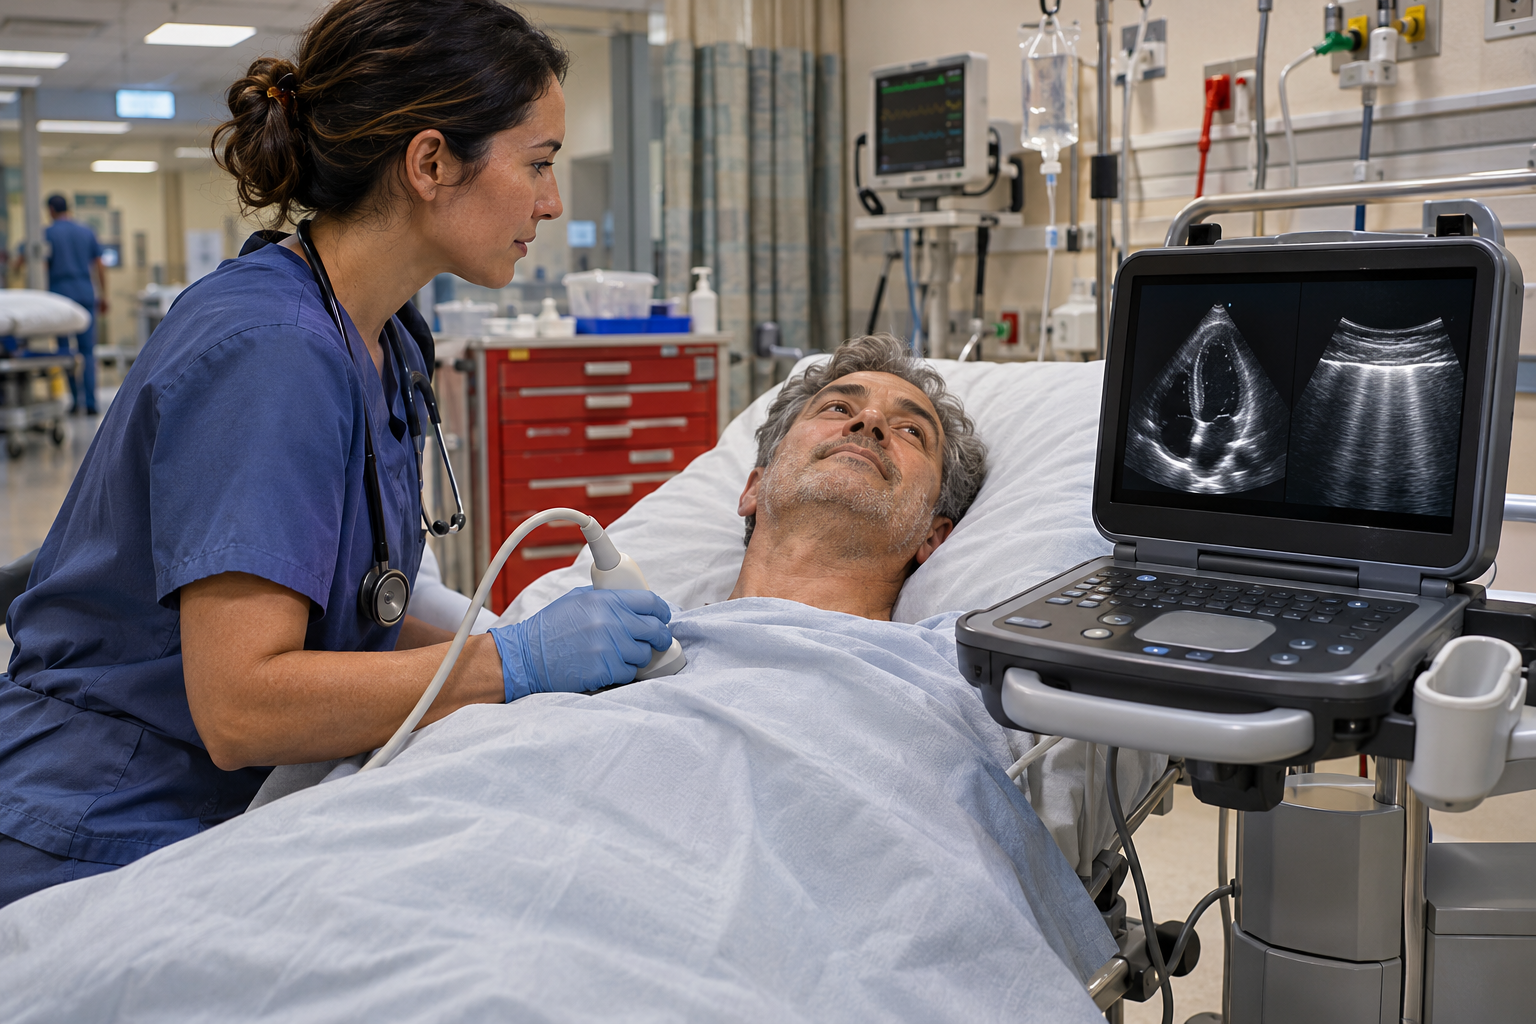
\includegraphics[width=\textwidth,keepaspectratio]{modalities/infographics/pocus_realistic.png}
\end{center}
\begin{center}\footnotesize POCUS is a focused bedside scan used to answer a defined clinical question; it does not replace a comprehensive examination when one is needed. AI-generated illustration; ultrasound panels are not clinical studies.\end{center}

\section{Overview}
Point-of-care ultrasound (POCUS) is a focused ultrasound examination performed and interpreted by a healthcare professional at the patient's bedside to answer specific clinical questions, guide procedures or monitor physiological changes.

Unlike comprehensive diagnostic ultrasonography, POCUS generally investigates a limited set of abnormalities to support immediate clinical decision-making. It is widely used in emergency medicine, critical care, anesthesiology, internal medicine, trauma care and rural healthcare.

\section{Where point-of-care ultrasound is used}

\subsection{Cardiovascular diseases}
\begin{enumerate}[leftmargin=*,itemsep=0.45em,topsep=0.4em]
\item \textbf{Acute myocardial infarction.} Useful imaging findings include: Possible regional wall motion abnormalities; requires clinical and diagnostic testing for assessment.
\item \textbf{Cardiac arrest.} Useful imaging findings include: Absence or presence of myocardial motion.
\item \textbf{Cardiac tamponade.} Useful imaging findings include: Pericardial effusion with right atrial or right ventricular collapse.
\item \textbf{Cardiogenic shock.} Useful imaging findings include: Reduced ventricular contractility or other cardiac abnormalities.
\item \textbf{Congestive heart failure.} Useful imaging findings include: Ventricular dysfunction, possible pulmonary B-lines and venous congestion.
\item \textbf{Dilated cardiomyopathy.} Useful imaging findings include: Enlarged ventricular chambers with reduced contractility.
\item \textbf{Hypertrophic cardiomyopathy.} Useful imaging findings include: Abnormal myocardial thickening.
\item \textbf{Hypovolemic shock.} Useful imaging findings include: Small, hyperdynamic left ventricle in selected patients.
\item \textbf{Infective endocarditis.} Useful imaging findings include: Possible visible vegetation; absence on POCUS does not exclude endocarditis, and comprehensive echocardiography is required.
\item \textbf{Intracardiac thrombus.} Useful imaging findings include: Possible abnormal intracardiac echogenic mass requiring confirmation with comprehensive imaging.
\item \textbf{Left ventricular aneurysm.} Useful imaging findings include: Focal ventricular wall thinning and abnormal motion.
\item \textbf{Left ventricular systolic dysfunction.} Useful imaging findings include: Reduced myocardial contractility.
\item \textbf{Obstructive shock.} Useful imaging findings include: Findings suggesting tamponade, pulmonary embolism or another obstruction.
\item \textbf{Pericardial effusion.} Useful imaging findings include: Anechoic fluid surrounding the heart.
\item \textbf{Pulmonary embolism.} Useful imaging findings include: Possible right ventricular dilatation and septal flattening; these indirect findings do not diagnose or exclude pulmonary embolism.
\item \textbf{Right ventricular dilatation.} Useful imaging findings include: Increased right-to-left ventricular size ratio.
\item \textbf{Right ventricular dysfunction.} Useful imaging findings include: Reduced right ventricular contractility.
\item \textbf{Septic shock.} Useful imaging findings include: Hyperdynamic or depressed ventricular contractility.
\item \textbf{Severe aortic stenosis.} Useful imaging findings include: Restricted or calcified aortic valve leaflets may raise suspicion; severity requires comprehensive echocardiography.
\item \textbf{Severe mitral regurgitation.} Useful imaging findings include: Possible abnormal regurgitant flow on color Doppler; severity requires comprehensive echocardiography.
\end{enumerate}
Focused cardiac ultrasound may raise suspicion for regional wall-motion abnormalities, vegetations, intracardiac thrombus or valve disease, but does not establish these diagnoses or reliably grade valve severity. Comprehensive echocardiography and clinical assessment are needed when these findings are suspected. A negative focused examination cannot exclude myocardial infarction, pulmonary embolism, endocarditis or significant valvular disease.

\subsection{Pulmonary and pleural diseases}
\begin{enumerate}[leftmargin=*,itemsep=0.45em,topsep=0.4em]
\item \textbf{Acute respiratory distress syndrome (ARDS).} Useful imaging findings include: Heterogeneous B-lines, irregular pleural line and spared regions.
\item \textbf{Aspiration pneumonia.} Useful imaging findings include: Dependent pulmonary consolidation.
\item \textbf{Cardiogenic pulmonary edema.} Useful imaging findings include: Frequently diffuse bilateral B-lines with relatively smooth pleural line.
\item \textbf{Diaphragmatic dysfunction.} Useful imaging findings include: Reduced diaphragmatic excursion or thickening.
\item \textbf{Diaphragmatic paralysis.} Useful imaging findings include: Absent or paradoxical diaphragmatic movement.
\item \textbf{Empyema.} Useful imaging findings include: Complex pleural collection with septations.
\item \textbf{Hemothorax.} Useful imaging findings include: Pleural fluid with variable internal echoes.
\item \textbf{Interstitial lung disease.} Useful imaging findings include: Multiple B-lines and pleural irregularities.
\item \textbf{Peripheral pulmonary abscess.} Useful imaging findings include: Complex fluid-containing pulmonary lesion accessible to ultrasound.
\item \textbf{Pleural effusion.} Useful imaging findings include: Anechoic or complex fluid above the diaphragm.
\item \textbf{Pleural malignancy.} Useful imaging findings include: Possible pleural nodularity and effusion.
\item \textbf{Pleural thickening.} Useful imaging findings include: Abnormally thickened pleural line.
\item \textbf{Pneumonia.} Useful imaging findings include: Subpleural consolidation with possible dynamic air bronchograms.
\item \textbf{Pneumothorax.} Useful imaging findings include: Absent lung sliding, absent B-lines and possible lung point.
\item \textbf{Pulmonary atelectasis.} Useful imaging findings include: Tissue-like consolidation with possible static air bronchograms.
\item \textbf{Pulmonary contusion.} Useful imaging findings include: Focal B-lines and subpleural consolidation.
\item \textbf{Pulmonary edema.} Useful imaging findings include: Multiple bilateral B-lines.
\item \textbf{Pulmonary fibrosis.} Useful imaging findings include: Irregular pleural surface and B-lines.
\item \textbf{Pulmonary infarction.} Useful imaging findings include: Possible peripheral wedge-shaped subpleural lesion.
\item \textbf{Viral pneumonia.} Useful imaging findings include: Patchy B-lines and subpleural abnormalities.
\end{enumerate}
Lung ultrasound primarily evaluates the pleural interface, artifacts and abnormalities extending to the lung periphery. It cannot comprehensively visualize normally aerated lung parenchyma.

\subsection{Vascular diseases}
\begin{enumerate}[leftmargin=*,itemsep=0.45em,topsep=0.4em]
\item \textbf{Abdominal aortic aneurysm.} Useful imaging findings include: Abdominal aortic diameter of at least 3 cm.
\item \textbf{Acute limb ischemia.} Useful imaging findings include: Reduced or absent arterial Doppler signals.
\item \textbf{Aortic dissection.} Useful imaging findings include: Possible intimal flap separating vascular lumens.
\item \textbf{Arterial pseudoaneurysm.} Useful imaging findings include: Vascular sac with characteristic to-and-fro flow at its neck.
\item \textbf{Arterial thrombosis.} Useful imaging findings include: Intraluminal material with absent or reduced flow.
\item \textbf{Arteriovenous fistula.} Useful imaging findings include: Abnormal communication with turbulent blood flow.
\item \textbf{Central venous congestion.} Useful imaging findings include: Venous dilatation and abnormal Doppler waveforms.
\item \textbf{Deep vein thrombosis.} Useful imaging findings include: Failure of venous compression.
\item \textbf{Femoral vein thrombosis.} Useful imaging findings include: Noncompressible femoral vein.
\item \textbf{Hepatic venous congestion.} Useful imaging findings include: Abnormal hepatic venous Doppler waveform.
\item \textbf{Iliac artery aneurysm.} Useful imaging findings include: Abnormal arterial dilatation.
\item \textbf{Peripheral arterial disease.} Useful imaging findings include: Abnormal arterial waveforms and vascular calcification.
\item \textbf{Popliteal vein thrombosis.} Useful imaging findings include: Noncompressible popliteal vein.
\item \textbf{Portal venous congestion.} Useful imaging findings include: Increased portal vein pulsatility.
\item \textbf{Renal venous congestion.} Useful imaging findings include: Discontinuous intrarenal venous flow.
\item \textbf{Superficial thrombophlebitis.} Useful imaging findings include: Noncompressible superficial vein with surrounding inflammation.
\item \textbf{Upper-extremity venous thrombosis.} Useful imaging findings include: Noncompressibility or abnormal venous Doppler flow.
\end{enumerate}
A negative focused ultrasound examination cannot reliably exclude aortic dissection or all forms of deep vein thrombosis.

\subsection{Trauma-related conditions}
\begin{enumerate}[leftmargin=*,itemsep=0.45em,topsep=0.4em]
\item \textbf{Abdominal wall hematoma.} Useful imaging findings include: Localized heterogeneous fluid collection.
\item \textbf{Hemoperitoneum.} Useful imaging findings include: Free intraperitoneal fluid.
\item \textbf{Hepatic injury.} Useful imaging findings include: Possible perihepatic fluid or abnormal hepatic echotexture.
\item \textbf{Intra-abdominal hemorrhage.} Useful imaging findings include: Free fluid in dependent abdominal spaces.
\item \textbf{Long-bone fracture.} Useful imaging findings include: Disruption of the hyperechoic bone surface.
\item \textbf{Renal trauma.} Useful imaging findings include: Possible perinephric fluid or hematoma.
\item \textbf{Rib fracture.} Useful imaging findings include: Discontinuity of the rib cortex.
\item \textbf{Splenic injury.} Useful imaging findings include: Possible perisplenic fluid or heterogeneous splenic tissue.
\item \textbf{Sternal fracture.} Useful imaging findings include: Cortical interruption or displacement.
\item \textbf{Traumatic cardiac tamponade.} Useful imaging findings include: Pericardial fluid with signs of impaired cardiac filling.
\item \textbf{Traumatic hemopericardium.} Useful imaging findings include: Pericardial fluid following trauma.
\item \textbf{Traumatic hemothorax.} Useful imaging findings include: Fluid within the pleural cavity.
\item \textbf{Traumatic muscle injury.} Useful imaging findings include: Disrupted muscle fibers and hematoma.
\item \textbf{Traumatic pneumothorax.} Useful imaging findings include: Abnormal lung sliding with possible lung point.
\end{enumerate}
FAST and eFAST primarily identify free fluid and selected thoracic abnormalities rather than directly identifying every injured organ. A negative examination does not exclude significant trauma.

\subsection{Hepatic and hepatobiliary diseases}
\begin{enumerate}[leftmargin=*,itemsep=0.45em,topsep=0.4em]
\item \textbf{Acalculous cholecystitis.} Useful imaging findings include: Gallbladder distension and inflammatory changes without stones.
\item \textbf{Acute cholecystitis.} Useful imaging findings include: Gallstones, wall thickening, pericholecystic fluid and sonographic Murphy sign.
\item \textbf{Ascites.} Useful imaging findings include: Free intraperitoneal fluid.
\item \textbf{Biliary obstruction.} Useful imaging findings include: Dilatation of the biliary tract.
\item \textbf{Choledocholithiasis.} Useful imaging findings include: Possible echogenic stone within the common bile duct.
\item \textbf{Cholelithiasis.} Useful imaging findings include: Echogenic gallstones with posterior acoustic shadowing.
\item \textbf{Gallbladder hydrops.} Useful imaging findings include: Marked gallbladder distension.
\item \textbf{Gallbladder sludge.} Useful imaging findings include: Low-level dependent intraluminal echoes.
\item \textbf{Hepatic abscess.} Useful imaging findings include: Complex heterogeneous fluid collection.
\item \textbf{Hepatic cyst.} Useful imaging findings include: Anechoic lesion with posterior acoustic enhancement.
\item \textbf{Hepatic steatosis.} Useful imaging findings include: Increased hepatic echogenicity.
\item \textbf{Hepatomegaly.} Useful imaging findings include: Increased liver dimensions.
\item \textbf{Liver cirrhosis.} Useful imaging findings include: Nodular hepatic surface and coarse echotexture.
\item \textbf{Portal hypertension.} Useful imaging findings include: Possible collateral vessels, splenomegaly and ascites.
\end{enumerate}

\subsection{Renal and urinary tract diseases}
\begin{enumerate}[leftmargin=*,itemsep=0.45em,topsep=0.4em]
\item \textbf{Acute kidney injury.} Useful imaging findings include: Possible obstruction or other structural renal abnormalities.
\item \textbf{Benign prostatic hyperplasia.} Useful imaging findings include: Enlarged prostate and possible urinary retention.
\item \textbf{Bladder blood clot.} Useful imaging findings include: Intraluminal echogenic material without internal vascularity.
\item \textbf{Bladder calculus.} Useful imaging findings include: Mobile echogenic structure with acoustic shadowing.
\item \textbf{Bladder diverticulum.} Useful imaging findings include: Fluid-filled outpouching communicating with the bladder.
\item \textbf{Bladder outlet obstruction.} Useful imaging findings include: Increased residual urine volume.
\item \textbf{Chronic kidney disease.} Useful imaging findings include: Small kidneys, increased echogenicity or cortical thinning.
\item \textbf{Hydronephrosis.} Useful imaging findings include: Dilatation of the renal collecting system.
\item \textbf{Nephrolithiasis.} Useful imaging findings include: Echogenic renal stone with acoustic shadowing.
\item \textbf{Obstructive uropathy.} Useful imaging findings include: Collecting system dilatation or bladder distension.
\item \textbf{Perinephric abscess.} Useful imaging findings include: Abnormal fluid collection surrounding the kidney.
\item \textbf{Polycystic kidney disease.} Useful imaging findings include: Multiple bilateral renal cysts.
\item \textbf{Renal abscess.} Useful imaging findings include: Focal complex fluid collection.
\item \textbf{Simple renal cyst.} Useful imaging findings include: Well-defined anechoic lesion.
\item \textbf{Ureterolithiasis.} Useful imaging findings include: Possible visible ureteral calculus and upstream hydronephrosis.
\item \textbf{Urinary retention.} Useful imaging findings include: Distended urinary bladder.
\end{enumerate}
POCUS is useful for detecting urinary obstruction but generally cannot establish the cause of intrinsic kidney disease.

\subsection{Gastrointestinal diseases}
\begin{enumerate}[leftmargin=*,itemsep=0.45em,topsep=0.4em]
\item \textbf{Acute appendicitis.} Useful imaging findings include: Enlarged, noncompressible blind-ending tubular structure.
\item \textbf{Acute diverticulitis.} Useful imaging findings include: Focal bowel wall thickening and inflamed surrounding fat.
\item \textbf{Appendiceal abscess.} Useful imaging findings include: Complex periappendiceal fluid collection.
\item \textbf{Appendicolith.} Useful imaging findings include: Echogenic appendiceal focus with posterior shadowing.
\item \textbf{Bowel ischemia.} Useful imaging findings include: Abnormal wall thickness, peristalsis or perfusion.
\item \textbf{Crohn disease.} Useful imaging findings include: Segmental bowel wall thickening and possible hypervascularity.
\item \textbf{Gastroenteritis.} Useful imaging findings include: Nonspecific fluid-filled loops and altered peristalsis.
\item \textbf{Gastrointestinal perforation.} Useful imaging findings include: Possible abnormal free-air artifacts.
\item \textbf{Hypertrophic pyloric stenosis.} Useful imaging findings include: Thickened and elongated pyloric muscle.
\item \textbf{Incarcerated hernia.} Useful imaging findings include: Nonreducible herniated contents.
\item \textbf{Inguinal hernia.} Useful imaging findings include: Protrusion of abdominal contents through an inguinal defect.
\item \textbf{Intra-abdominal abscess.} Useful imaging findings include: Localized complex fluid collection.
\item \textbf{Intussusception.} Useful imaging findings include: Target or doughnut sign.
\item \textbf{Large bowel obstruction.} Useful imaging findings include: Colonic dilatation.
\item \textbf{Paralytic ileus.} Useful imaging findings include: Dilated bowel loops with reduced peristalsis.
\item \textbf{Small bowel obstruction.} Useful imaging findings include: Dilated fluid-filled bowel loops with abnormal peristalsis.
\item \textbf{Ulcerative colitis.} Useful imaging findings include: Colonic wall thickening.
\item \textbf{Umbilical hernia.} Useful imaging findings include: Abdominal contents extending through an umbilical defect.
\end{enumerate}

\subsection{Obstetric diseases and conditions}
\begin{enumerate}[leftmargin=*,itemsep=0.45em,topsep=0.4em]
\item \textbf{Anembryonic pregnancy.} Useful imaging findings include: Empty gestational sac meeting diagnostic size criteria.
\item \textbf{Breech presentation.} Useful imaging findings include: Fetal buttocks or feet directed toward the cervix.
\item \textbf{Early pregnancy loss.} Useful imaging findings include: Findings meeting validated criteria for pregnancy nonviability.
\item \textbf{Ectopic pregnancy.} Useful imaging findings include: Possible extrauterine gestational sac or adnexal mass.
\item \textbf{Fetal cardiac activity.} Useful imaging findings include: Visible rhythmic fetal cardiac motion.
\item \textbf{Intrauterine fetal demise.} Useful imaging findings include: Absent fetal cardiac activity meeting confirmation requirements.
\item \textbf{Intrauterine pregnancy.} Useful imaging findings include: Intrauterine gestational sac containing a yolk sac or embryo.
\item \textbf{Low-lying placenta.} Useful imaging findings include: Possible placental edge near the internal cervical opening; confirm with dedicated obstetric ultrasound.
\item \textbf{Molar pregnancy.} Useful imaging findings include: Abnormal heterogeneous intrauterine tissue with cystic spaces.
\item \textbf{Multiple pregnancy.} Useful imaging findings include: Multiple embryos or gestational sacs.
\item \textbf{Oligohydramnios.} Useful imaging findings include: Reduced amniotic fluid volume.
\item \textbf{Placenta previa.} Useful imaging findings include: Possible placenta covering the internal cervical opening on a bedside scan; confirm with dedicated obstetric ultrasound.
\item \textbf{Polyhydramnios.} Useful imaging findings include: Increased amniotic fluid volume.
\item \textbf{Pregnancy of unknown location.} Useful imaging findings include: No definite intrauterine or extrauterine pregnancy identified.
\item \textbf{Retained products of conception.} Useful imaging findings include: Abnormal intrauterine tissue with variable vascularity.
\item \textbf{Ruptured ectopic pregnancy.} Useful imaging findings include: Possible adnexal abnormality with hemoperitoneum.
\item \textbf{Subchorionic hematoma.} Useful imaging findings include: Crescent-shaped collection adjacent to the gestational sac.
\item \textbf{Transverse fetal lie.} Useful imaging findings include: Fetal longitudinal axis perpendicular to maternal axis.
\end{enumerate}
POCUS does not replace comprehensive antenatal ultrasound, fetal anomaly screening or formal assessment of uncertain pregnancy viability. Suspected placenta previa or low-lying placenta requires dedicated obstetric imaging; transvaginal ultrasound may be needed for accurate localization.

\subsection{Gynecological diseases}
\begin{enumerate}[leftmargin=*,itemsep=0.45em,topsep=0.4em]
\item \textbf{Adenomyosis.} Useful imaging findings include: Heterogeneous myometrium with possible small cystic spaces.
\item \textbf{Endometrial thickening.} Useful imaging findings include: Increased endometrial thickness.
\item \textbf{Hematometra.} Useful imaging findings include: Fluid or blood distending the endometrial cavity.
\item \textbf{Hemorrhagic ovarian cyst.} Useful imaging findings include: Reticular internal echoes or retracting clot.
\item \textbf{Hydrosalpinx.} Useful imaging findings include: Elongated fluid-filled tubular adnexal structure.
\item \textbf{Ovarian endometrioma.} Useful imaging findings include: Homogeneous low-level internal echoes.
\item \textbf{Ovarian torsion.} Useful imaging findings include: Enlarged ovary with peripheral follicles and possible twisted vascular pedicle.
\item \textbf{Pelvic inflammatory disease.} Useful imaging findings include: Possible tubal thickening and pelvic fluid.
\item \textbf{Ruptured ovarian cyst.} Useful imaging findings include: Adnexal lesion with pelvic free fluid.
\item \textbf{Simple ovarian cyst.} Useful imaging findings include: Anechoic adnexal lesion.
\item \textbf{Tubo-ovarian abscess.} Useful imaging findings include: Complex inflammatory adnexal mass.
\item \textbf{Uterine fibroids.} Useful imaging findings include: Well-defined solid myometrial masses.
\end{enumerate}
Preserved ovarian Doppler flow does not exclude ovarian torsion.

\subsection{Male reproductive disorders}
\begin{enumerate}[leftmargin=*,itemsep=0.45em,topsep=0.4em]
\item \textbf{Epididymal cyst.} Useful imaging findings include: Well-defined anechoic epididymal lesion.
\item \textbf{Epididymitis.} Useful imaging findings include: Enlarged hypervascular epididymis.
\item \textbf{Epididymo-orchitis.} Useful imaging findings include: Increased epididymal and testicular vascularity.
\item \textbf{Hematocele.} Useful imaging findings include: Complex hemorrhagic scrotal fluid collection.
\item \textbf{Hydrocele.} Useful imaging findings include: Anechoic fluid surrounding the testis.
\item \textbf{Orchitis.} Useful imaging findings include: Enlarged hypervascular testis.
\item \textbf{Pyocele.} Useful imaging findings include: Complex infected scrotal collection.
\item \textbf{Testicular hematoma.} Useful imaging findings include: Focal heterogeneous intratesticular collection.
\item \textbf{Testicular mass.} Useful imaging findings include: Discrete intratesticular lesion.
\item \textbf{Testicular rupture.} Useful imaging findings include: Disrupted testicular contour and heterogeneous parenchyma.
\item \textbf{Testicular torsion.} Useful imaging findings include: Reduced or absent testicular perfusion and possible whirlpool sign.
\item \textbf{Varicocele.} Useful imaging findings include: Dilated pampiniform venous plexus.
\end{enumerate}

\subsection{Musculoskeletal diseases}
\begin{enumerate}[leftmargin=*,itemsep=0.45em,topsep=0.4em]
\item \textbf{Achilles tendinopathy.} Useful imaging findings include: Tendon thickening and altered fibrillar architecture.
\item \textbf{Achilles tendon rupture.} Useful imaging findings include: Tendon discontinuity and retraction.
\item \textbf{Baker cyst.} Useful imaging findings include: Fluid collection between characteristic posterior knee structures.
\item \textbf{Bursitis.} Useful imaging findings include: Fluid within a bursal space.
\item \textbf{Calcific tendinitis.} Useful imaging findings include: Echogenic intratendinous calcification.
\item \textbf{Calcium pyrophosphate deposition disease.} Useful imaging findings include: Hyperechoic deposits within cartilage.
\item \textbf{Clavicle fracture.} Useful imaging findings include: Cortical discontinuity.
\item \textbf{Foreign body.} Useful imaging findings include: Echogenic structure with variable shadowing or reverberation.
\item \textbf{Gout.} Useful imaging findings include: Double-contour sign and possible tophaceous deposits.
\item \textbf{Joint effusion.} Useful imaging findings include: Anechoic or hypoechoic intra-articular fluid.
\item \textbf{Muscle hematoma.} Useful imaging findings include: Heterogeneous intramuscular collection.
\item \textbf{Muscle tear.} Useful imaging findings include: Disruption of normal muscle fibers.
\item \textbf{Osteoarthritis.} Useful imaging findings include: Osteophytes and irregular articular margins.
\item \textbf{Patellar tendon rupture.} Useful imaging findings include: Discontinuity of patellar tendon fibers.
\item \textbf{Plantar fasciitis.} Useful imaging findings include: Thickened hypoechoic plantar fascia.
\item \textbf{Quadriceps tendon rupture.} Useful imaging findings include: Disrupted quadriceps tendon architecture.
\item \textbf{Radial head fracture.} Useful imaging findings include: Cortical disruption or associated joint effusion.
\item \textbf{Rheumatoid arthritis.} Useful imaging findings include: Synovial hypertrophy and increased Doppler vascularity.
\item \textbf{Rotator cuff tear.} Useful imaging findings include: Focal tendon defect or complete discontinuity.
\item \textbf{Rotator cuff tendinopathy.} Useful imaging findings include: Tendon thickening and heterogeneous echogenicity.
\item \textbf{Septic arthritis.} Useful imaging findings include: Joint effusion with possible synovial inflammatory changes.
\item \textbf{Shoulder dislocation.} Useful imaging findings include: Abnormal humeral head position relative to glenoid.
\item \textbf{Tenosynovitis.} Useful imaging findings include: Tendon sheath fluid and increased vascularity.
\item \textbf{Trigger finger.} Useful imaging findings include: A1 pulley thickening and abnormal tendon movement.
\end{enumerate}
Ultrasound cannot reliably distinguish septic arthritis from sterile inflammatory joint effusions without clinical assessment and, when indicated, joint aspiration.

\subsection{Skin and soft-tissue diseases}
\begin{enumerate}[leftmargin=*,itemsep=0.45em,topsep=0.4em]
\item \textbf{Cellulitis.} Useful imaging findings include: Cobblestone appearance of subcutaneous tissue.
\item \textbf{Cutaneous abscess.} Useful imaging findings include: Complex fluid collection with internal debris.
\item \textbf{Epidermoid cyst.} Useful imaging findings include: Well-defined lesion with variable internal echoes.
\item \textbf{Hidradenitis suppurativa.} Useful imaging findings include: Dermal thickening, fluid collections and sinus tracts.
\item \textbf{Lipoma.} Useful imaging findings include: Relatively well-defined superficial fatty lesion.
\item \textbf{Necrotizing fasciitis.} Useful imaging findings include: Possible fascial fluid, thickening or soft-tissue gas.
\item \textbf{Pilonidal abscess.} Useful imaging findings include: Complex subcutaneous collection near the natal cleft.
\item \textbf{Pyomyositis.} Useful imaging findings include: Abnormal muscle echotexture with possible intramuscular abscess.
\item \textbf{Retained foreign body.} Useful imaging findings include: Echogenic structure with surrounding inflammatory reaction.
\item \textbf{Seroma.} Useful imaging findings include: Localized simple or mildly complex fluid collection.
\item \textbf{Soft-tissue hematoma.} Useful imaging findings include: Heterogeneous collection with evolving echogenicity.
\item \textbf{Soft-tissue mass.} Useful imaging findings include: Discrete lesion with variable echogenicity and vascularity.
\item \textbf{Subcutaneous edema.} Useful imaging findings include: Hypoechoic fluid separating fat lobules.
\item \textbf{Subcutaneous emphysema.} Useful imaging findings include: Reverberation artifacts caused by soft-tissue gas.
\end{enumerate}
A negative POCUS examination must not be used to exclude necrotizing fasciitis.

\subsection{Ophthalmological diseases}
\begin{enumerate}[leftmargin=*,itemsep=0.45em,topsep=0.4em]
\item \textbf{Choroidal detachment.} Useful imaging findings include: Thick, smooth, dome-shaped peripheral membranes.
\item \textbf{Endophthalmitis.} Useful imaging findings include: Vitreous debris and inflammatory abnormalities.
\item \textbf{Intraocular mass.} Useful imaging findings include: Focal solid intraocular lesion.
\item \textbf{Lens dislocation.} Useful imaging findings include: Abnormal lens position.
\item \textbf{Optic nerve sheath distension.} Useful imaging findings include: Increased optic nerve sheath diameter.
\item \textbf{Orbital cellulitis.} Useful imaging findings include: Possible orbital inflammatory changes or collection.
\item \textbf{Papilledema.} Useful imaging findings include: Possible optic disc protrusion into the vitreous cavity.
\item \textbf{Posterior vitreous detachment.} Useful imaging findings include: Mobile vitreous membrane with variable attachments.
\item \textbf{Retinal detachment.} Useful imaging findings include: Echogenic membrane commonly tethered to the optic disc.
\item \textbf{Retrobulbar hemorrhage.} Useful imaging findings include: Abnormal retrobulbar collection.
\item \textbf{Vitreous degeneration.} Useful imaging findings include: Mobile vitreous opacities.
\item \textbf{Vitreous hemorrhage.} Useful imaging findings include: Mobile low-level echoes within the vitreous cavity.
\end{enumerate}
Ocular POCUS has important limitations. It cannot establish glaucoma, reliably quantify intracranial pressure or replace a complete eye examination. Ultrasound should generally be avoided when an open-globe injury is suspected.

\subsection{Neurological and neurovascular conditions}
\begin{enumerate}[leftmargin=*,itemsep=0.45em,topsep=0.4em]
\item \textbf{Carotid artery stenosis.} Useful imaging findings include: Abnormal arterial narrowing and velocity elevations.
\item \textbf{Carpal tunnel syndrome.} Useful imaging findings include: Increased median nerve cross-sectional area.
\item \textbf{Cerebral circulatory arrest.} Useful imaging findings include: Characteristic reverberating flow or systolic spikes under validated protocols.
\item \textbf{Cerebral hypoperfusion.} Useful imaging findings include: Reduced cerebral blood flow velocities.
\item \textbf{Cerebral vasospasm.} Useful imaging findings include: Increased cerebral arterial Doppler velocities.
\item \textbf{Intracranial arterial stenosis.} Useful imaging findings include: Abnormal focal Doppler velocities.
\item \textbf{Peripheral nerve compression.} Useful imaging findings include: Nerve enlargement at the site of compression.
\item \textbf{Peripheral nerve injury.} Useful imaging findings include: Abnormal fascicular architecture or discontinuity.
\item \textbf{Suspected elevated intracranial pressure.} Useful imaging findings include: Possible increased optic nerve sheath diameter.
\item \textbf{Ulnar neuropathy.} Useful imaging findings include: Focal ulnar nerve enlargement.
\end{enumerate}
Transcranial Doppler and nerve ultrasound require specialized training beyond basic POCUS protocols.

\subsection{Pediatric and neonatal conditions}
\begin{enumerate}[leftmargin=*,itemsep=0.45em,topsep=0.4em]
\item \textbf{Developmental dysplasia of the hip.} Useful imaging findings include: Assessed with dedicated, standardized hip ultrasound; not usually diagnosed by general POCUS.
\item \textbf{Hydrocephalus.} Useful imaging findings include: Ventricular enlargement.
\item \textbf{Hypertrophic pyloric stenosis.} Useful imaging findings include: Increased pyloric muscle thickness and length.
\item \textbf{Intraventricular hemorrhage.} Useful imaging findings include: Abnormal echogenic material within cerebral ventricles.
\item \textbf{Necrotizing enterocolitis.} Useful imaging findings include: Abnormal bowel wall appearance, pneumatosis or portal venous gas.
\item \textbf{Neonatal pneumonia.} Useful imaging findings include: Pulmonary consolidation and abnormal pleural findings.
\item \textbf{Neonatal pneumothorax.} Useful imaging findings include: Absent lung sliding and possible lung point.
\item \textbf{Neonatal respiratory distress syndrome.} Useful imaging findings include: Diffuse B-lines and abnormal pleural appearance.
\item \textbf{Pediatric appendicitis.} Useful imaging findings include: Enlarged noncompressible appendix.
\item \textbf{Pediatric dehydration.} Useful imaging findings include: Possible cardiovascular and vascular changes; nonspecific.
\item \textbf{Pediatric intussusception.} Useful imaging findings include: Target-shaped bowel lesion.
\item \textbf{Pediatric urinary obstruction.} Useful imaging findings include: Hydronephrosis or bladder abnormalities.
\item \textbf{Transient tachypnea of the newborn.} Useful imaging findings include: Interstitial lung ultrasound pattern.
\item \textbf{Umbilical catheter malposition.} Useful imaging findings include: Abnormal catheter tip position.
\end{enumerate}
Neonatal cranial and hip ultrasound are dedicated examinations that may be performed at the bedside by trained clinicians; they should not be conflated with routine focused POCUS protocols.

\subsection{Airway and anesthesiology-related conditions}
\begin{enumerate}[leftmargin=*,itemsep=0.45em,topsep=0.4em]
\item \textbf{Diaphragmatic dysfunction.} Useful imaging findings include: Reduced diaphragmatic excursion.
\item \textbf{Difficult airway anatomy.} Useful imaging findings include: Abnormal airway dimensions or landmarks.
\item \textbf{Endotracheal tube malposition.} Useful imaging findings include: Abnormal airway or unilateral lung ventilation findings.
\item \textbf{Esophageal intubation.} Useful imaging findings include: Double-tract appearance on tracheal ultrasound.
\item \textbf{Gastric fluid retention.} Useful imaging findings include: Anechoic or hypoechoic gastric antral contents.
\item \textbf{Gastric solid contents.} Useful imaging findings include: Heterogeneous echogenic gastric contents.
\item \textbf{Hemidiaphragmatic paralysis.} Useful imaging findings include: Absent or paradoxical diaphragmatic motion.
\item \textbf{Increased aspiration risk.} Useful imaging findings include: Gastric contents suggesting a nonempty stomach.
\item \textbf{Upper airway edema.} Useful imaging findings include: Possible soft-tissue thickening.
\item \textbf{Vocal cord paralysis.} Useful imaging findings include: Reduced or absent vocal fold movement.
\end{enumerate}
Waveform capnography remains the standard method for confirming and continuously monitoring tracheal intubation.

\subsection{Fluid status and critical care assessment}
\begin{enumerate}[leftmargin=*,itemsep=0.45em,topsep=0.4em]
\item \textbf{Acute circulatory failure.} Useful imaging findings include: Abnormal cardiac function or vascular volume-related findings.
\item \textbf{Fluid overload.} Useful imaging findings include: Pulmonary B-lines, pleural effusions and venous congestion.
\item \textbf{Fluid-responsive circulatory dysfunction.} Useful imaging findings include: Increased stroke volume following a dynamic preload challenge.
\item \textbf{Hypervolemia.} Useful imaging findings include: Possible venous congestion and pulmonary B-lines.
\item \textbf{Hypovolemia.} Useful imaging findings include: Possible small hyperdynamic ventricle and reduced venous dimensions.
\item \textbf{Postoperative fluid collection.} Useful imaging findings include: Localized abnormal fluid accumulation.
\item \textbf{Pulmonary congestion.} Useful imaging findings include: Multiple pulmonary B-lines.
\item \textbf{Respiratory muscle dysfunction.} Useful imaging findings include: Reduced diaphragmatic thickening or excursion.
\item \textbf{Right-sided heart failure.} Useful imaging findings include: Right ventricular abnormalities and systemic venous congestion.
\item \textbf{Sepsis-induced cardiomyopathy.} Useful imaging findings include: Global ventricular systolic dysfunction.
\item \textbf{Systemic venous congestion.} Useful imaging findings include: Dilated inferior vena cava and abnormal venous Doppler patterns.
\item \textbf{Weaning-associated pulmonary edema.} Useful imaging findings include: Increasing B-lines during spontaneous breathing trials.
\end{enumerate}
Inferior vena cava diameter and collapsibility should not be used alone to determine hydration status or predict fluid responsiveness.

\subsection{Summary of catalogue}
\begin{tabular}{@{}p{0.70\textwidth}r@{}}
\toprule
\textbf{Disease category} & \textbf{Entries} \\
\midrule
Airway and anesthesiology-related conditions & 10 \\
Cardiovascular diseases & 20 \\
Fluid status and critical care assessment & 12 \\
Gastrointestinal diseases & 18 \\
Gynecological diseases & 12 \\
Hepatic and hepatobiliary diseases & 14 \\
Male reproductive disorders & 12 \\
Musculoskeletal diseases & 24 \\
Neurological and neurovascular conditions & 10 \\
Obstetric diseases and conditions & 18 \\
Ophthalmological diseases & 12 \\
Pediatric and neonatal conditions & 14 \\
Pulmonary and pleural diseases & 20 \\
Renal and urinary tract diseases & 16 \\
Skin and soft-tissue diseases & 14 \\
Trauma-related conditions & 14 \\
Vascular diseases & 17 \\
\midrule
\textbf{Total} & \textbf{257} \\
\bottomrule
\end{tabular}

\subsection{Standardized POCUS protocols}
POCUS commonly uses structured examination protocols designed to answer specific clinical questions.

\begin{longtable}{@{}p{0.2\textwidth}p{0.4\textwidth}p{0.34\textwidth}@{}}
\toprule
\textbf{Protocol} & \textbf{Full name} & \textbf{Primary clinical application} \\
\midrule
\endfirsthead
\toprule
\textbf{Protocol} & \textbf{Full name} & \textbf{Primary clinical application} \\
\midrule
\endhead
BLUE & Bedside Lung Ultrasound in Emergency & Acute respiratory failure \\
CASA & Cardiac Arrest Sonographic Assessment & Cardiac arrest evaluation \\
Diaphragmatic ultrasound & Focused diaphragm assessment & Respiratory muscle function \\
DVT compression ultrasound & Focused venous compression examination & Deep vein thrombosis \\
eFAST & Extended Focused Assessment with Sonography in Trauma & Trauma, pneumothorax and hemothorax \\
FALLS & Fluid Administration Limited by Lung Sonography & Ultrasound-assisted circulatory failure assessment \\
FAST & Focused Assessment with Sonography in Trauma & Intraperitoneal and pericardial fluid \\
FATE & Focus-Assessed Transthoracic Echocardiography & Focused cardiac assessment \\
FEEL & Focused Echocardiographic Evaluation in Life Support & Cardiac arrest \\
FoCUS & Focused Cardiac Ultrasound & Cardiac structure and function \\
Gastric POCUS & Focused gastric ultrasound & Gastric contents and aspiration risk \\
RUSH & Rapid Ultrasound in Shock and Hypotension & Undifferentiated shock \\
VExUS & Venous Excess Ultrasound Score & Systemic venous congestion \\
\bottomrule
\end{longtable}

\subsection{Characteristic sonographic signs}
\begin{longtable}{@{}p{0.35\textwidth}p{0.59\textwidth}@{}}
\toprule
\textbf{Sonographic sign} & \textbf{Associated disease or condition} \\
\midrule
\endfirsthead
\toprule
\textbf{Sonographic sign} & \textbf{Associated disease or condition} \\
\midrule
\endhead
A-lines & Normally aerated lung or other A-line-predominant patterns \\
B-lines & Increased peripheral lung density or reduced aeration \\
Barcode sign & Absent lung sliding on M-mode \\
Cobblestone sign & Subcutaneous edema or cellulitis \\
D-sign & Right ventricular pressure or volume overload \\
Double-contour sign & Gout \\
Double-tract sign & Esophageal intubation \\
Dynamic air bronchogram & Supports pneumonia rather than obstructive atelectasis \\
Kissing papillary muscles & Small hyperdynamic left ventricular cavity \\
Lung point & Pneumothorax \\
McConnell sign & Regional right ventricular dysfunction \\
Posterior acoustic enhancement & Fluid-containing structures \\
Posterior acoustic shadowing & Stones, calcifications and other strongly attenuating structures \\
Seashore sign & Lung sliding on M-mode \\
Shred sign & Peripheral pulmonary consolidation \\
Sonographic Murphy sign & Supports acute cholecystitis \\
Spine sign above diaphragm & Pleural fluid or consolidation \\
Target sign & Intussusception \\
Tissue-like sign & Pulmonary consolidation \\
To-and-fro waveform & Pseudoaneurysm neck \\
Twinkling artifact & Urinary calculi or other reflective interfaces \\
Whirlpool sign & Twisting of a vascular pedicle \\
Yin-yang sign & Turbulent bidirectional vascular flow within a sac \\
\bottomrule
\end{longtable}
Many sonographic signs are not pathognomonic and must be interpreted in the clinical context.

\subsection{Ultrasound transducers used in POCUS}
\begin{longtable}{@{}p{0.28\textwidth}p{0.25\textwidth}p{0.41\textwidth}@{}}
\toprule
\textbf{Transducer} & \textbf{Typical frequency} & \textbf{Applications} \\
\midrule
\endfirsthead
\toprule
Broadband handheld transducer & Device-dependent & Multiple bedside applications \\
\midrule
\endhead
Curvilinear array & 2--6 MHz & Abdominal, renal, obstetric and trauma imaging \\
Endocavitary & 5--12 MHz & Transvaginal and pelvic imaging \\
Linear array & 7--18 MHz & Vascular, musculoskeletal, soft tissue and ocular imaging \\
Microconvex array & 3--10 MHz & Pediatric and selected abdominal imaging \\
Phased array & 1--5 MHz & Cardiac and thoracic imaging \\
\textbf{Transducer} & \textbf{Typical frequency} & \textbf{Applications} \\
\bottomrule
\end{longtable}

\subsection{Quantitative POCUS parameters}
\begin{longtable}{@{}p{0.39\textwidth}p{0.14\textwidth}p{0.41\textwidth}@{}}
\toprule
\textbf{Parameter} & \textbf{Abbreviation} & \textbf{Clinical application} \\
\midrule
\endfirsthead
\toprule
\textbf{Parameter} & \textbf{Abbreviation} & \textbf{Clinical application} \\
\midrule
\endhead
Abdominal aortic diameter & AAD & Abdominal aortic aneurysm \\
Appendiceal diameter & --- & Appendicitis assessment \\
Bladder volume & BV & Urinary retention \\
Cardiac output & CO & Circulatory function \\
Common bile duct diameter & CBD & Biliary obstruction assessment \\
Diaphragmatic excursion & DE & Diaphragm function \\
Diaphragmatic thickening fraction & DTF & Respiratory muscle contraction \\
Gallbladder wall thickness & GBWT & Gallbladder inflammation assessment \\
Gastric antral cross-sectional area & CSA & Gastric volume estimation \\
Inferior vena cava collapsibility index & IVCCI & Respiratory venous diameter variation during spontaneous breathing \\
Inferior vena cava diameter & IVC & Supplementary hemodynamic assessment \\
Left ventricular ejection fraction & LVEF & Ventricular systolic function \\
Left ventricular outflow tract velocity-time integral & LVOT VTI & Stroke volume estimation \\
Lung ultrasound score & LUS & Pulmonary aeration assessment \\
Median nerve cross-sectional area & CSA & Carpal tunnel assessment \\
Optic nerve sheath diameter & ONSD & Supplementary intracranial pressure assessment \\
Postvoid residual volume & PVR & Bladder emptying \\
Right-to-left ventricular diameter ratio & RV/LV & Right ventricular enlargement \\
Tricuspid annular plane systolic excursion & TAPSE & Right ventricular systolic function \\
Venous excess ultrasound score & VExUS & Systemic venous congestion \\
\bottomrule
\end{longtable}

\subsection{Common bedside calculations}
Stroke volume can be estimated from left ventricular outflow tract area and velocity-time integral:
\[
SV=\pi\left(\frac{D_{\mathrm{LVOT}}}{2}\right)^2\times VTI_{\mathrm{LVOT}}
\]
Cardiac output is estimated as:
\[
CO=SV\times HR
\]
Inferior vena cava collapsibility index is calculated as:
\[
IVCCI=\frac{D_{\max}-D_{\min}}{D_{\max}}\times100
\]
This collapsibility formulation is intended for spontaneous breathing. During positive-pressure ventilation, a distensibility measure may be used instead; interpretation remains dependent on the clinical context.
Diaphragmatic thickening fraction is calculated as:
\[
DTF=\frac{T_{\mathrm{inspiration}}-T_{\mathrm{expiration}}}{T_{\mathrm{expiration}}}\times100
\]
A common urinary bladder volume approximation is:
\[
V\approx0.52\times L\times W\times H
\]
These measurements depend on acquisition quality, patient physiology and the assumptions of each model.

\subsection{POCUS-guided medical procedures}
\begin{longtable}{@{}p{0.47\textwidth}p{0.47\textwidth}@{}}
\toprule
\textbf{Procedure} & \textbf{Primary application} \\
\midrule
\endfirsthead
\toprule
\textbf{Procedure} & \textbf{Primary application} \\
\midrule
\endhead
Abscess drainage & Localization and drainage of infected collections \\
Arterial catheterization & Hemodynamic monitoring \\
Arthrocentesis & Joint fluid aspiration \\
Bursal injection & Targeted therapeutic injection \\
Central venous catheterization & Central vascular access \\
Chest tube placement & Pleural space localization \\
Fascia iliaca block & Regional pain management \\
Foreign body removal & Localization of retained material \\
Fracture reduction assessment & Evaluation of bone alignment \\
Joint injection & Image-guided intra-articular treatment \\
Lumbar puncture & Anatomical landmark identification \\
Paracentesis & Ascitic fluid aspiration \\
Pericardiocentesis & Pericardial fluid drainage \\
Peripheral intravenous catheterization & Difficult peripheral vascular access \\
Peripheral nerve block & Regional anesthesia \\
Suprapubic catheterization & Bladder localization \\
Tendon sheath injection & Targeted therapeutic injection \\
Thoracentesis & Pleural fluid aspiration \\
Transversus abdominis plane block & Abdominal wall analgesia \\
\bottomrule
\end{longtable}

\subsection{POCUS versus comprehensive ultrasonography}
\begin{longtable}{@{}p{0.29\textwidth}p{0.31\textwidth}p{0.34\textwidth}@{}}
\toprule
\textbf{Feature} & \textbf{POCUS} & \textbf{Comprehensive diagnostic ultrasound} \\
\midrule
\endfirsthead
\toprule
\textbf{Feature} & \textbf{POCUS} & \textbf{Comprehensive diagnostic ultrasound} \\
\midrule
\endhead
Anatomical coverage & Targeted & Systematic \\
Clinical interpretation & Frequently immediate & Typically formal reporting \\
Diagnostic completeness & Limited by focused examination & Generally greater \\
Equipment & Handheld, portable or conventional & Generally dedicated ultrasound systems \\
Examination duration & Frequently a few minutes & Frequently 15--60 minutes \\
Examination location & Usually bedside & Usually dedicated imaging department \\
Operator & Appropriately trained treating clinician & Sonographer or imaging specialist \\
Operator dependence & High & High \\
Physical mechanism & Ultrasound & Ultrasound \\
Primary objective & Answer focused clinical questions & Comprehensive anatomical and pathological assessment \\
Procedural guidance & Extensive & Extensive in appropriate specialties \\
Serial examination & Easily performed & Possible, but less convenient \\
Suitability for remote healthcare & Excellent & Equipment and staffing dependent \\
\bottomrule
\end{longtable}

\subsection{Published datasets and professional resources}
\begin{longtable}{@{}p{0.49\textwidth}p{0.45\textwidth}@{}}
\toprule
\textbf{Resource} & \textbf{Primary application} \\
\midrule
\endfirsthead
\toprule
\textbf{Resource} & \textbf{Primary application} \\
\midrule
\endhead
American College of Emergency Physicians & Emergency ultrasound clinical guidelines \\
American Institute of Ultrasound in Medicine & Ultrasound practice parameters and safety \\
American Society of Echocardiography & Cardiac ultrasound recommendations \\
CAMUS Dataset & Cardiac ultrasound segmentation \\
EchoNet-Dynamic & Cardiac ultrasound video analysis \\
Grand Challenge & Medical imaging research challenges \\
PhysioNet & Physiological and clinical research datasets \\
POCUS Atlas & Clinical POCUS images and videos \\
PubMed Central & Published clinical ultrasound images and research \\
Radiopaedia & Annotated medical imaging cases \\
Society of Critical Care Medicine & Critical care ultrasonography \\
UltrasoundCases.info & Clinical ultrasound case images \\
World Federation for Ultrasound in Medicine and Biology & International ultrasound standards \\
\bottomrule
\end{longtable}
EchoNet-Dynamic and CAMUS contain echocardiographic data rather than exclusively bedside POCUS acquisitions.

\subsection{Recommended metadata for a POCUS dataset}
\begin{longtable}{@{}p{0.45\textwidth}p{0.49\textwidth}@{}}
\toprule
\textbf{Attribute} & \textbf{Example} \\
\midrule
Acquisition depth & 5 cm \\
Acquisition format & Video \\
Acquisition mode & B-mode and M-mode \\
Anatomical region & Anterior chest \\
Associated artifact & Barcode sign \\
Clinical setting & Emergency department \\
Diagnostic question & Is a pneumothorax present? \\
Disease & Pneumothorax \\
Examination protocol & eFAST \\
File format & DICOM or MP4 \\
Frame rate & 30 fps \\
Image annotation & Pleural line segmentation \\
Image license & Specified license \\
Imaging modality & Point-of-care ultrasound \\
Laterality & Right \\
Patient position & Supine \\
Primary finding & Absent lung sliding \\
Publication reference & DOI or PMID \\
Reference standard & CT-confirmed pneumothorax \\
Secondary finding & Lung point \\
Temporal annotation & Respiratory cycle \\
Transducer & Linear array \\
Transducer frequency & 10 MHz \\
\bottomrule
\end{longtable}
The example values are illustrative, not measurements from an actual patient.

\subsection{Artificial intelligence applications in POCUS}
\begin{longtable}{@{}p{0.47\textwidth}p{0.47\textwidth}@{}}
\toprule
\textbf{AI application} & \textbf{Computational task} \\
\midrule
\endfirsthead
\toprule
\textbf{AI application} & \textbf{Computational task} \\
\midrule
\endhead
Abdominal free fluid detection & Image classification and segmentation \\
Anatomical landmark identification & Keypoint detection \\
Automated diagnostic reporting & Multimodal language modeling \\
B-line detection and counting & Object detection \\
Bladder volume estimation & Geometric image analysis \\
Cardiac chamber segmentation & Semantic segmentation \\
Cardiac ejection fraction estimation & Video regression \\
Cardiac view recognition & Image classification \\
Deep vein thrombosis detection & Compression video analysis \\
Fetal cardiac activity detection & Temporal signal analysis \\
Gallstone detection & Object detection \\
Hydronephrosis grading & Ordinal classification \\
Image quality assessment & Quality classification \\
Needle localization & Object tracking \\
Pericardial effusion detection & Object detection \\
Pleural line segmentation & Semantic segmentation \\
Pneumothorax detection & Spatiotemporal classification \\
Probe positioning guidance & Spatial navigation \\
Pulmonary consolidation detection & Object detection \\
Ultrasound acquisition guidance & Real-time feedback \\
\bottomrule
\end{longtable}

\subsection{POCUS data dimensionality}
\begin{longtable}{@{}p{0.42\textwidth}p{0.52\textwidth}@{}}
\toprule
\textbf{Acquisition technique} & \textbf{Data dimensionality} \\
\midrule
\endfirsthead
\toprule
\textbf{Acquisition technique} & \textbf{Data dimensionality} \\
\midrule
\endhead
Color Doppler & X, Y, velocity, time \\
Compression ultrasonography & X, Y, time, applied compression \\
Four-dimensional ultrasound & X, Y, Z, time \\
M-mode & Depth, time \\
Real-time B-mode & X, Y, time \\
Serial POCUS examinations & Imaging data, clinical measurements, examination time \\
Spectral Doppler & Velocity, time, signal intensity \\
Static B-mode & X, Y \\
Three-dimensional ultrasound & X, Y, Z \\
\bottomrule
\end{longtable}

\subsection{Established versus investigational applications}
\begin{longtable}{@{}p{0.45\textwidth}p{0.49\textwidth}@{}}
\toprule
\textbf{Application} & \textbf{Clinical status} \\
\midrule
Clinical application & Clinical status \\
Clinical application & Clinical status \\
Abdominal aortic aneurysm detection & Established \\
Appendicitis assessment & Established in trained settings \\
Autonomous AI-based disease diagnosis & Investigational \\
FAST and eFAST & Established \\
Focused cardiac ultrasound & Established \\
Gallstone detection & Established \\
Gastric ultrasound & Specialized clinical application \\
Hydronephrosis detection & Established \\
Intrauterine pregnancy confirmation & Established \\
Musculoskeletal injury assessment & Specialized clinical application \\
Ocular ultrasound & Specialized clinical application \\
Optic nerve sheath-based intracranial pressure estimation & Supplementary application \\
Pleural effusion detection & Established \\
Pneumothorax assessment & Established \\
Proximal deep vein thrombosis assessment & Established \\
Pulmonary edema assessment & Established \\
Robotic autonomous POCUS acquisition & Emerging research application \\
Soft-tissue abscess detection & Established \\
Ultrasound-guided vascular access & Established \\
Urinary retention assessment & Established \\
Venous congestion assessment using VExUS & Emerging clinical application \\
\bottomrule
\end{longtable}

\subsection{Medical imaging taxonomy}
POCUS is a clinical application of ultrasound rather than an independent physical imaging modality. A useful hierarchy is:

\begin{verbatim}
Ultrasound
|-- Conventional diagnostic ultrasound
|-- Doppler ultrasound
|-- Echocardiography
|-- Endoscopic ultrasound
|-- Contrast-enhanced ultrasound
|-- Ultrasound elastography
`-- Point-of-care ultrasound
    |-- Cardiac POCUS
    |-- Pulmonary POCUS
    |-- Abdominal POCUS
    |-- Vascular POCUS
    |-- Trauma POCUS
    |-- Obstetric POCUS
    |-- Musculoskeletal POCUS
    |-- Ocular POCUS
    |-- Pediatric POCUS
    `-- Procedural POCUS
\end{verbatim}

For machine-learning research, POCUS is question-driven, dynamic and closely integrated with clinical decision-making. Video sequences, clinical indications, acquisition protocols and independently confirmed diagnoses are generally more informative than isolated static images.

 Some entries overlap, some require specialized ultrasound training, and individual entries and resource links have not been independently validated against published clinical guidelines.





% ============================================================
% PART III. IMAGE INTERPRETATION
% ============================================================
\part{Image Interpretation}

\chapter{Pattern Recognition in Imaging}

\section*{Patient focus}
This chapter explains the examination or clinical problem in accessible language. Patients should use it to prepare questions and understand the purpose, experience, benefits, and limitations of imaging; local instructions and the official report take priority.


\label{ch:ch29_pattern_recognition}

\section{A Structured Approach}
Begin with the clinical question, compare prior studies, confirm technical adequacy, and identify the modality and sequence. Review anatomy systematically before focusing on the most conspicuous abnormality. Separate observation from interpretation and interpretation from recommendation.

\subsection{The Systematic Search Pattern}
Rather than scanning images haphazardly, adopt a consistent search pattern for every study. On a chest CT, for example, begin with the airways, then the lungs, pleura, mediastinum, heart, vessels, bones, and soft tissues. On a brain MRI, assess symmetry, then grey--white differentiation, ventricles, sulci, and extra-axial spaces. A reproducible approach reduces the chance of missing incidental or unexpected findings.

\begin{pearlbox}[Clinical Pearl: Always check the edge]
A preventable source of missed findings is incomplete image review. Lung apices, the posterior costophrenic sulcus, visible upper-abdominal structures on chest CT, and the skull vault on brain imaging can be overlooked. Build ``edge checks'' into your routine.
\end{pearlbox}

\section{Pattern Families}
Describe location, distribution, morphology, attenuation or signal, enhancement, diffusion, temporal behavior, and associated findings. Pattern recognition narrows a differential but does not replace clinical correlation or tissue diagnosis when required.

\subsection{Common Radiological Patterns}

Table~\ref{tab:pattern_families} summarises the principal pattern families encountered in everyday practice and the differential diagnoses they most commonly suggest.

\begin{table}[h]
\centering
\caption{Common imaging patterns and their principal differential diagnoses.}
\label{tab:pattern_families}
\begin{tabular}{p{3.2cm} p{4cm} p{5.5cm}}
\toprule
\textbf{Pattern} & \textbf{Distribution / Features} & \textbf{Key Differentials} \\
\midrule
Consolidation & Dense opacification obscuring vessels, air bronchograms & Pneumonia, organising pneumonia, pulmonary infarction, lymphoma \\
Cystic lung disease & Multiple thin- or thick-walled cysts & Lymphangioleiomyomatosis, pulmonary Langerhans cell histiocytosis, Birt--Hogg--Dub\'{e} syndrome \\
Diffuse bilateral infiltrates & Symmetrical or asymmetrical airspace or interstitial pattern & ARDS, pulmonary oedema, diffuse alveolar haemorrhage, miliary TB \\
Ground-glass opacity & Hazy increase in attenuation with preservation of bronchovascular margins & Pneumocystis pneumonia, viral pneumonia, pulmonary oedema, alveolar haemorrhage, adenocarcinoma in situ \\
Multiple lytic lesions & Widespread, ``punched-out'' & Multiple myeloma, metastases (thyroid, renal, breast, lung), hyperparathyroidism \\
Multiple pulmonary nodules & Random, perilymphatic, or centrilobular & Metastases, septic emboli, granulomatous disease, vasculitis \\
Solitary bone lesion & Lytic, blastic, or mixed & Metastasis, myeloma, enchondroma, fibrous dysplasia, simple bone cyst \\
Solitary pulmonary nodule & Round, $\leq 3$~cm, well or poorly defined & Granuloma, hamartoma, primary lung carcinoma, metastasis, AVM \\
\bottomrule
\end{tabular}
\end{table}

\subsection{Characterising a Lesion by Pattern}
For any lesion, systematically evaluate:
\begin{enumerate}
    \item \textbf{Location} -- organ, lobe, segment, compartment.
    \item \textbf{Morphology} -- round, irregular, spiculated, cystic, solid.
    \item \textbf{Attenuation / Signal} -- fat, water, soft tissue, air, bone, haemorrhage.
    \item \textbf{Enhancement} -- none, peripheral, nodular, homogeneous, heterogeneous.
    \item \textbf{Margins} -- well-defined, ill-defined, infiltrative.
    \item \textbf{Effect on adjacent structures} -- mass effect, bone destruction, vessel encasement.
\end{enumerate}
These attributes narrow the differential and guide the next investigation.

\begin{pearlbox}[Clinical Pearl: Interpret morphology and size together]
Nodule assessment considers size, morphology, attenuation, calcification pattern, interval growth, and patient risk. A tiny spiculated nodule and a larger calcified nodule cannot be ranked reliably from size or a generic description of calcification alone; use the full imaging and clinical context and applicable management guidance.
\end{pearlbox}

\section{Cognitive Safety}
Use a checklist, deliberately search for common missed findings, and reconsider the first impression when discordant evidence appears. Avoid anchoring, premature closure, search satisfaction, and overconfidence. Escalate uncertain or critical findings according to local policy.

\subsection{Common Cognitive Biases in Radiology}

\begin{table}[h]
\centering
\caption{Cognitive biases most relevant to imaging interpretation.}
\label{tab:cognitive_biases}
\begin{tabular}{p{3.5cm} p{9cm}}
\toprule
\textbf{Bias} & \textbf{Description and Example} \\
\midrule
Anchoring & Over-reliance on the first piece of information. A ``known'' pneumonia on the referral may cause the reader to miss an underlying mass. \\
Availability bias & Overweighting diagnoses seen recently. After reading about COVID-19 pneumonia, every ground-glass opacity is attributed to viral infection. \\
Confirmation bias & Seeking information that supports a preferred diagnosis while ignoring contradicting evidence. \\
Overconfidence & Failing to seek a second opinion or acknowledge uncertainty when clinical stakes are high. \\
Premature closure & Accepting a diagnosis before all findings are accounted for. Labeling a focal opacity as pneumonia without considering an obstructing lesion when the clinical or imaging features do not fit. \\
Search satisfaction & Finding one abnormality and stopping the search. A positive CT pulmonary angiogram may distract from an additional lung mass or pneumothorax. \\
\bottomrule
\end{tabular}
\end{table}

\subsection{Practical Steps to Reduce Error}
\begin{itemize}
    \item Always compare with prior imaging when available.
    \item Use a structured checklist for high-risk examinations (e.g.\ CT pulmonary angiography, trauma CT).
    \item Discuss uncertain cases with a colleague before finalising the report.
    \item When an unexpected finding is identified, complete the full search pattern rather than jumping to the obvious abnormality.
    \item Be explicit about uncertainty in the report rather than using vague language.
\end{itemize}

\begin{pearlbox}[Impression:]
Pattern recognition is the backbone of radiological interpretation. A systematic search pattern, awareness of common cognitive biases, and a willingness to question your first impression will substantially reduce diagnostic error.
\end{pearlbox}

\clearpage

\chapter{Imaging Anatomy}

\label{ch:ch30_anatomy}

\section{Anatomic Orientation}
Interpretation requires knowledge of normal compartmental anatomy, planes, vascular territories, organ relationships, and expected age- or procedure-related variation. Confirm orientation and laterality before describing a lesion.

\subsection{Axial, Coronal, and Sagittal Planes}
All cross-sectional images can be understood in three orthogonal planes:
\begin{itemize}
    \item \textbf{Axial (transverse)} -- divides the body into superior and inferior halves. The standard viewing convention is from below (feet looking up), so the patient's right is on the viewer's left.
    \item \textbf{Coronal} -- divides the body into anterior and posterior halves. Useful for assessing the adrenal glands, thoracic inlet, and hip joints.
    \item \textbf{Sagittal} -- divides the body into left and right halves. Essential for spine, sternum, and midline structures such as the pituitary gland.
\end{itemize}

\subsection{Identifying Level on a Single Image}
When given a single axial image, you can determine the approximate level by identifying key landmarks:
\begin{itemize}
    \item \textbf{Supraclavicular} -- clavicle heads, lung apices, great vessels.
    \item \textbf{Aortic arch level} -- aortic arch, SVC, and trachea.
    \item \textbf{Carina} -- tracheal bifurcation, main bronchi, and nearby pulmonary arteries.
    \item \textbf{Cardiac level} -- cardiac chambers and pericardium; valve detail depends on slice position and reconstruction plane.
    \item \textbf{Liver dome} -- liver, IVC, hepatic veins.
    \item \textbf{Renal hilum} -- kidneys and renal vessels; the pancreatic body may be visible anteriorly.
    \item \textbf{Aortic bifurcation} -- common iliac vessels, sacrum.
\end{itemize}

\begin{pearlbox}[Clinical Pearl: One image, one level]
If you can identify the trachea, a great vessel, and a vertebral body, you can determine the approximate axial level within seconds. Practice this skill on every CT you read.
\end{pearlbox}

\section{Cross-Sectional Anatomy by Region}

\subsection{Brain}
On CT, grey matter is denser (lighter) than white matter. On MRI, T1-weighted images show white matter as brighter than grey matter, while T2-weighted images reverse this relationship. The ventricular system, basal ganglia, thalami, brainstem, and cerebellum should be identified on every brain study. The major vascular territories---anterior cerebral, middle cerebral, posterior cerebral, and vertebrobasilar---correspond to specific cortical and deep structures.

\subsection{Chest}
Key structures on axial CT of the chest include the trachea and main bronchi, the mediastinal great vessels (ascending aorta, descending aorta, SVC, and pulmonary arteries), the heart and pericardium, the lung parenchyma with its lobes and fissures, the pleura, the oesophagus, and the thoracic spine. On sagittal reconstructions, the aortic arch and main pulmonary artery are useful orientation landmarks.

\subsection{Abdomen}
The abdomen is divided into nine regions or four quadrants for clinical description. On axial CT, systematically identify the liver, spleen, pancreas, kidneys, adrenal glands, bowel loops, mesentery, and retroperitoneum. A portal-venous phase, often acquired around 60--70~s after contrast injection, is commonly used to assess abdominal parenchymal organs; timing and additional phases depend on the clinical question and protocol.

\subsection{Pelvis}
The pelvis contains the bladder, reproductive organs, rectum, and the pelvic floor musculature. On MRI, the zonal anatomy of the uterus (endometrium, junctional zone, myometrium) and the peripheral zone of the prostate are best assessed on T2-weighted images.

\section{Cross-Modality Correlation}
CT, MRI, ultrasound, radiography, and nuclear medicine depict different physical properties. A structure that is conspicuous on one examination may be occult on another. Correlate with the modality best suited to the clinical question.

\begin{table}[h]
\centering
\caption{Best modality for specific anatomic questions.}
\label{tab:anatomy_modality}
\begin{tabular}{p{5cm} p{4cm} p{4.5cm}}
\toprule
\textbf{Clinical Question} & \textbf{Preferred Modality} & \textbf{Why} \\
\midrule
Aortic dissection & CTA & Rapid, volumetric coverage with excellent spatial resolution \\
Bone cortex and fracture & CT or radiography & High spatial resolution for calcified structures \\
Brain parenchyma detail & MRI (T2/FLAIR/DWI) & Soft-tissue contrast resolution \\
Hip labrum & MRI; MR arthrography in selected cases & Soft-tissue assessment of the labrum and adjacent structures \\
Liver lesion characterisation & MRI with hepatobiliary contrast in selected cases & Hepatobiliary-phase features can help distinguish focal nodular hyperplasia from many adenomas, but some adenomas also retain contrast \\
Pulmonary nodules & Chest CT; low-dose for screening or follow-up when appropriate & High spatial resolution for lung parenchyma; protocol depends on the clinical question \\
\bottomrule
\end{tabular}
\end{table}

\section{Reporting}
Use precise location, side, compartment, dimensions, and relationship to critical structures. State when an organ or region is incompletely visualized. Normal anatomy should be described only to the degree necessary to support the clinical question and exclude important pathology.

\begin{pearlbox}[Clinical Pearl: Know the blood supply]
Vascular territory can help narrow the differential. A pleural-based wedge-shaped consolidation may suggest pulmonary infarction, particularly when pulmonary embolism is suspected, but it can overlap with infection and other causes. Interpret it with the full imaging pattern and clinical context.
\end{pearlbox}

\clearpage

\chapter{Normal Variants and Anatomic Mimics}

\label{ch:ch31_normal_variants}

\section{Definition}
A normal variant is a benign anatomic, developmental, physiologic, or technical appearance that may mimic disease. Variants can be common, uncommon, or clinically important in a particular context.

\subsection{Why Variants Matter}
Normal variants cause two problems: they may be \textbf{mistaken for pathology} (leading to unnecessary investigation or anxiety), or they may \textbf{mask genuine disease} (because the reader assumes the finding is a known variant). Recognising variants requires knowledge of anatomy, developmental biology, and the imaging characteristics that distinguish benign from malignant.

\section{Common Normal Variants}

\begin{table}[h]
\centering
\caption{Common normal variants by body region.}
\label{tab:normal_variants}
\begin{tabular}{p{3.5cm} p{3.5cm} p{7cm}}
\toprule
\textbf{Region} & \textbf{Variant} & \textbf{Key Features} \\
\midrule
Brain & Falx cerebri calcification & Linear or nodular calcification along the interhemispheric fissure; increases with age \\
Brain & Choroid plexus calcification & Often bilateral and symmetric in the glomus of the lateral ventricles; commonly physiologic in adults and more frequent with age \\
Brain & Prominent arachnoid granulations (Pacchioni) & Smooth, well-defined, CSF-intensity lesions along the superior sagittal sinus; may erode the inner table of the skull \\
Chest & Dextrocardia & Mirror-image cardiac position; situs inversus if abdominal organs are also reversed \\
Kidney & Dromedary hump & Focal contour prominence of the left kidney due to splenic impression; shows normal enhancement \\
Liver & Prominent caudate lobe & May be a normal anatomic configuration, but caudate enlargement can also occur with chronic liver disease; assess the whole liver and clinical context \\
Musculoskeletal & Accessory ossification centers & Persistent unfused centers (e.g.\ os acromiale, bipartite patella) with smooth, well-corticated margins; bilaterality varies by variant \\
Spleen & Accessory spleen & Usually a small, well-defined nodule near the splenic hilum or pancreatic tail that typically follows splenic signal and enhancement \\
\bottomrule
\end{tabular}
\end{table}

\begin{pearlbox}[Clinical Pearl: Accessory spleen vs. recurrence]
After splenectomy for selected haematologic conditions, residual accessory splenic tissue or splenosis may contribute to persistent or recurrent disease. When clinically relevant, assess the splenic bed and consider possible ectopic sites. Such tissue often resembles the spleen in signal and enhancement, but size and appearance vary; indeterminate lesions may need confirmatory imaging.
\end{pearlbox}

\section{Safe Recognition}
Use age, symptoms, prior imaging, distribution, enhancement, and stability. Do not label an appearance as a variant solely because it is unfamiliar. If a lesion is indeterminate or has suspicious features, recommend appropriate further evaluation rather than reassurance.

\subsection{Distinguishing Variants from Pathology}
The following features favour a normal variant:
\begin{itemize}
    \item \textbf{Characteristic location} -- a dromedary hump is typically a contour bulge along the lateral midportion of the left kidney, related to splenic impression.
    \item \textbf{Characteristic morphology} -- accessory ossification centers typically have smooth, well-corticated margins at an expected ossification site; correlate with age, symptoms and trauma history.
    \item \textbf{Relationship to parent tissue} -- an accessory spleen usually has signal and enhancement similar to the spleen, although the match may vary with size, phase and technique.
    \item \textbf{Stability} -- long-term stability can support a benign variant, but stability alone does not prove that a finding is benign.
    \item \textbf{Bilaterality} -- bilateral findings can support some variants, but bilaterality alone does not establish that a finding is benign.
\end{itemize}

\subsection{When to Recommend Follow-Up}
If a finding does not meet the criteria above, do not dismiss it as a variant. Recommend follow-up imaging or further characterisation when:
\begin{itemize}
    \item The patient has symptoms or risk factors for malignancy.
    \item The morphology is atypical for a known variant.
    \item There is no prior imaging for comparison.
    \item The finding has changed in size or appearance.
\end{itemize}

\begin{pearlbox}[Clinical Pearl: Os acromiale]
Os acromiale is an unfused ossification center of the acromion that can be confused with an acromial fracture. Smooth, well-corticated margins at a typical location support a variant; assess for acute injury and correlate with symptoms. Bilaterality may support the diagnosis but is not required.
\end{pearlbox}

\section{Communication}
Explain the distinguishing features and any relevant caveat. Avoid implying that every variant is harmless in every patient; some variants alter procedural risk or are associated with disease in selected settings.

\subsection{Structured Reporting of a Suspected Variant}
When reporting a finding that you believe to be a normal variant:
\begin{enumerate}
    \item State the finding clearly and provide measurements.
    \item Describe the features that support it being a variant (location, morphology, signal characteristics).
    \item State whether prior imaging is available for comparison.
    \item If confident, state ``consistent with normal variant'' and recommend no further follow-up.
    \item If uncertain, recommend targeted follow-up and state the specific concern.
\end{enumerate}

\begin{pearlbox}[Impression:]
Many normal variants have no clinical consequence, but some affect procedural planning or are relevant in particular diseases. Recognition should use the full pattern of location, morphology, signal or attenuation, enhancement, prior imaging and clinical context; no single feature proves a finding is benign. When uncertain, recommend appropriate further evaluation rather than reassurance.
\end{pearlbox}

\clearpage

\chapter{Imaging Artifacts}

\label{ch:ch32_artifacts}

\section{Common Sources}
Artifacts arise from motion, metal, beam hardening, partial volume, truncation, aliasing, susceptibility, flow, reverberation, attenuation correction, misregistration, and reconstruction or display errors.

\subsection{Why Artifacts Occur}
Imaging artifacts are features that do not accurately represent the anatomy or physiology being examined. They can arise from the physics of image acquisition, patient motion, limitations in sampling or reconstruction, and image processing or display. Understanding their causes helps you recognize artifacts, reduce them when possible, and avoid mistaking them for disease.

\section{CT Artifacts}

\begin{table}[h]
\centering
\caption{Common CT artifacts: causes, appearance, and management.}
\label{tab:ct_artifacts}
\begin{tabular}{p{3cm} p{3.5cm} p{3.5cm} p{4cm}}
\toprule
\textbf{Artifact} & \textbf{Cause} & \textbf{Appearance} & \textbf{Management} \\
\midrule
Beam hardening & Preferential absorption of lower-energy photons along paths through dense structures & Dark bands or streaks, often between dense structures such as the petrous bones & Use an appropriate higher-kVp or spectral protocol and validated beam-hardening correction; increasing mAs may help when photon starvation also contributes \\
Metal streak & Metal-related beam hardening, photon starvation, scatter and edge effects & Bright and dark streaks radiating from the metal object & Consider scanner-specific metal-artifact reduction, higher kVp or spectral techniques; protocol adjustments depend on the scanner and clinical task \\
Motion & Patient movement during acquisition & Blurring, step-like misalignment or duplicated edges & Use coaching, immobilization or a shorter acquisition where appropriate; repeat only when needed and clinically justified \\
Partial volume & A voxel contains more than one tissue or structure & Averaged attenuation that obscures small structures or blurs boundaries & Use thinner acquired or reconstructed slices when appropriate; this may increase image noise \\
Truncation & Part of the patient lies outside the reconstruction field of view & Shading, streaks or distortion near the image periphery & Center the patient and select an adequate field of view; use extended-field reconstruction when available \\
\bottomrule
\end{tabular}
\end{table}

\begin{pearlbox}[Clinical Pearl: Metal is everywhere]
Dental fillings, sternotomy wires, surgical clips, and hip prostheses all cause streak artifacts. When interpreting post-surgical imaging, always check whether a region of interest is degraded by adjacent metal before calling a finding.
\end{pearlbox}

\section{MRI Artifacts}

\begin{table}[h]
\centering
\caption{Common MRI artifacts: causes, appearance, and management.}
\label{tab:mri_artifacts}
\begin{tabular}{p{3cm} p{3.5cm} p{3.5cm} p{4cm}}
\toprule
\textbf{Artifact} & \textbf{Cause} & \textbf{Appearance} & \textbf{Management} \\
\midrule
Chemical shift & Frequency difference between fat and water protons & Bright or dark band at fat--water interfaces (in-plane or slice-select direction) & Increase receiver bandwidth, use fat--water separation techniques \\
Motion (ghosting) & Periodic motion (cardiac, respiratory, flowing blood) & Signal replicated in the phase-encoding direction & Use cardiac gating, respiratory triggering, navigator echoes, or motion-robust sequences \\
Susceptibility & Local magnetic field inhomogeneity at tissue interfaces or near metal & Signal void, geometric distortion; exaggerated on gradient-echo and susceptibility-weighted sequences & Use spin-echo sequences, increase bandwidth, apply metal artefact reduction sequences (MARS) \\
Truncation (Gibbs ringing) & Finite sampling of k-space at a sharp boundary & Parallel bright and dark lines near high-contrast interfaces (e.g.\ CSF--brain interface) & Acquire higher spatial resolution when appropriate or use k-space filtering/apodisation, recognizing that filtering can blur detail; zero-filling only interpolates the image \\
Wrap-around (aliasing) & Anatomy outside the field of view is undersampled and folds into the image & Duplicate structures overlaid on the image of interest & Increase the field of view, use phase oversampling/no-phase-wrap, change the phase-encoding direction, or apply saturation bands as appropriate \\
\bottomrule
\end{tabular}
\end{table}

\begin{pearlbox}[Clinical Pearl: Phase-encoding direction]
Motion ghosts commonly appear along the phase-encoding direction, although appearance depends on the sequence and source of motion. If you see suspicious linear signal along the anterior--posterior axis on an axial brain image, consider whether it could be a respiratory ghost before calling it a lesion.
\end{pearlbox}

\section{Ultrasound Artifacts}

\begin{table}[h]
\centering
\caption{Common ultrasound artifacts.}
\label{tab:us_artifacts}
\begin{tabular}{p{3cm} p{4cm} p{7cm}}
\toprule
\textbf{Artifact} & \textbf{Cause} & \textbf{Appearance and Significance} \\
\midrule
Mirror image & Sound reflected from a strong curved reflector creates a duplicate image & A ``second'' lesion on the opposite side of the reflector; classically liver lesion mirrored across the diaphragm \\
Posterior acoustic enhancement & Reduced attenuation through a fluid-containing or otherwise low-attenuation structure & Increased brightness deep to the structure; supports fluid content but is not by itself definitive for a cyst \\
Posterior acoustic shadowing & Strong reflection or attenuation by structures such as stones, calcification, gas or bone & Reduced echoes deep to the structure; may support a stone or calcification when the location and other findings are compatible, but is not specific \\
Refraction & Sound beam bent at interfaces of different propagation speeds & Displacement of structures; can simulate duplication of vessels or organs \\
Reverberation & Sound bouncing repeatedly between two strong reflectors & Equally spaced horizontal lines deep to the reflector; can simulate bowel gas or foreign bodies \\
\bottomrule
\end{tabular}
\end{table}

\section{Recognition}
An artifact often follows a predictable geometry, crosses tissue boundaries, or changes between sequences, planes, reconstructions, or repeat acquisitions. Compare raw or alternative images when available and correlate with anatomy and clinical findings.

\subsection{Checklist for Artifact Recognition}
\begin{enumerate}
    \item Does the finding follow a known artifact pattern (streak, ghost, reverberation)?
    \item Does it change on different sequences, phases, or planes?
    \item Is it anatomically plausible, or does it cross tissue boundaries unnaturally?
    \item Is there a technical explanation (metal, motion, field-of-view limitation)?
    \item Does it correspond to a clinical finding on examination?
\end{enumerate}

\section{Management}
Report limitations that could affect diagnosis. Repeat or supplement imaging only when it is likely to change management and after considering dose, contrast, and patient burden. Never interpret an artifact as disease without checking its behavior and technical explanation.

\begin{pearlbox}[Impression:]
Artifacts are inherent to every imaging modality. Recognising the characteristic appearance and cause of each artifact prevents misdiagnosis. When in doubt, check whether the finding changes across sequences, planes, or repeat acquisitions before attributing clinical significance.
\end{pearlbox}

\clearpage

\chapter{Imaging Measurements and Quantification}

\label{ch:ch33_measurements}

\section{Measurement Principles}
Measure in the plane and sequence that best depicts the target, use consistent landmarks, record units, and distinguish longest dimension from volumetric or orthogonal measurements. State whether a value is approximate and whether technique limits precision.

\subsection{Best Practices}
\begin{itemize}
    \item Use the \textbf{same modality, protocol, plane, and method} for serial comparisons when feasible; if they differ, document the limitation.
    \item Use \textbf{electronic calipers} rather than ruler-on-screen measurements.
    \item Report measurements in \textbf{millimetres} (lesions) or \textbf{centimetres} (organs).
    \item Document the \textbf{level} or \textbf{plane} in which the measurement was made.
    \item Measure nodules according to the relevant organ-specific guideline; some systems use a mean of orthogonal diameters or volumetry rather than the single longest diameter.
\end{itemize}

\section{Common Measurements}

\begin{table}[h]
\centering
\caption{Common imaging measurements, reference values, and clinical significance.}
\label{tab:common_measurements}
\begin{tabular}{p{3.2cm} p{2.8cm} p{3.2cm} p{4.5cm}}
\toprule
\textbf{Measurement} & \textbf{Modality} & \textbf{Normal / Threshold} & \textbf{Clinical Significance} \\
\midrule
Aortic diameter & CT or MRI, measured perpendicular to vessel centerline & Ascending aorta $\geq4.0$~cm is generally considered dilated in an average-sized adult & Interpret by segment, body size, and clinical context; intervention thresholds depend on aortic disease and patient-specific risk \\
Cardiothoracic ratio & Upright PA chest X-ray & Usually $\leq0.5$ in adults & A ratio above 0.5 may suggest cardiac enlargement; it is not reliable on AP or supine films and is not a diagnosis by itself \\
CTPA right-to-left ventricular ratio & CTPA & RV/LV ratio around or above 1 may indicate right ventricular enlargement/strain & Used for PE risk assessment; it does not diagnose PE severity alone, and is not the RPA/LPA diameter ratio \\
Liver span & US or CT & Technique- and body-size-dependent; a midclavicular span around 10--15~cm is a rough reference & Interpret with body habitus, lobe shape, and other findings; no single length establishes hepatomegaly \\
Renal length & US or CT & Often approximately 9--12~cm in adults; varies with body size and age & Small kidneys may occur in chronic disease; hydronephrosis is identified by collecting-system dilatation, not kidney length alone \\
T-score (DXA) & DXA & $\geq -1.0$ is normal; $<-1.0$ to $>-2.5$ is low bone mass; $\leq-2.5$ is osteoporosis & Apply diagnostic T-score criteria at validated skeletal sites in populations for whom they are intended; interpret with clinical risk \\
Vertebral body height & Lateral radiograph or sagittal CT/MRI & Height loss of about 20\% or more may meet a vertebral fracture grading threshold & Assess vertebral shape and endplates and exclude non-fracture deformity; height loss alone does not establish cause \\
\bottomrule
\end{tabular}
\end{table}

\section{Lexicon-Based Assessment Systems}
Several validated lexicons standardise the reporting of specific organs. Each provides a defined vocabulary, assessment categories, and management recommendations.

\subsection{BI-RADS (Breast Imaging Reporting and Data System)}
The ACR BI-RADS system uses seven final assessment categories, numbered 0--6:
\begin{enumerate}
    \item \textbf{BI-RADS 0} -- Incomplete; requires additional imaging.
    \item \textbf{BI-RADS 1} -- Negative; no abnormalities.
    \item \textbf{BI-RADS 2} -- Benign findings.
    \item \textbf{BI-RADS 3} -- Probably benign; short-term follow-up recommended ($<2\%$ malignancy risk).
    \item \textbf{BI-RADS 4} -- Suspicious; tissue diagnosis is generally recommended (4A: $>2$--$\leq10\%$, 4B: $>10$--$\leq50\%$, 4C: $>50$--$<95\%$ likelihood of malignancy).
    \item \textbf{BI-RADS 5} -- Highly suggestive of malignancy ($\geq95\%$ likelihood).
    \item \textbf{BI-RADS 6} -- Known biopsy-proven malignancy, used when imaging is performed after diagnosis.
\end{enumerate}

\subsection{Lung-RADS (Lung CT Screening Reporting and Data System)}
Lung-RADS is used for lung cancer screening CT. Version 2022 includes categories 0, 1, 2, 3, 4A, 4B, and 4X. Category assignment depends on nodule type, size, whether it is new or growing, and other imaging features; thresholds and management are defined in the current ACR table. In brief:
\begin{itemize}
    \item \textbf{Category 0} -- Incomplete; additional imaging or comparison with prior studies is needed.
    \item \textbf{Category 1} -- Negative or definitely benign.
    \item \textbf{Category 2} -- Benign appearance or behavior; routine screening interval.
    \item \textbf{Category 3} -- Probably benign; short-interval screening follow-up.
    \item \textbf{Category 4A} -- Suspicious; short-interval follow-up, with PET/CT considered for a sufficiently large solid nodule or solid component.
    \item \textbf{Category 4B} -- Very suspicious; diagnostic evaluation is recommended, selected according to clinical context.
    \item \textbf{Category 4X} -- Category 3 or 4 nodule with additional imaging features that increase suspicion.
\end{itemize}

\subsection{TI-RADS (Thyroid Imaging Reporting and Data System)}
ACR TI-RADS assigns points based on composition, echogenicity, shape, margin, and echogenic foci of thyroid nodules. The total score determines the TI-RADS level (TR1--TR5), which guides fine-needle aspiration recommendations and ultrasound follow-up intervals.

\subsection{PI-RADS (Prostate Imaging Reporting and Data System)}
PI-RADS v2.1 uses a 1--5 scale for suspicious lesions on multiparametric MRI of the prostate. The score is determined primarily by DWI in the peripheral zone and T2-weighted imaging in the transition zone. PI-RADS 5 indicates a very high probability of clinically significant prostate cancer.

\subsection{LI-RADS (Liver Imaging Reporting and Data System)}
Diagnostic CT/MRI LI-RADS is intended for adults in defined high-risk groups, including most patients with cirrhosis, selected patients with chronic hepatitis B, and patients with current or prior hepatocellular carcinoma. It classifies observations from LR-1 (definitely benign) through LR-5 (definitely HCC in the eligible population), with LR-M for probably or definitely malignant but not specific for HCC, and LR-TIV for tumor in vein. Eligibility and exclusions should be checked before assigning a category.

\section{Change Over Time}
Compare like with like: same modality, protocol, plane, and measurement method when possible. Small differences may reflect reader or technical variability. Growth thresholds and follow-up intervals are disease- and guideline-specific.

\subsection{Interobserver Variability}
All measurements are subject to inter- and intraobserver variability. CT nodule measurements can vary between readers and acquisition protocols. Some guidelines use an increase of at least 2~mm in diameter or more than 25\% in volume as a growth criterion, but these thresholds are not universal and depend on the nodule type, measurement method, and guideline.

\begin{pearlbox}[Clinical Pearl: Volume doubling time]
For pulmonary nodules, volumetric growth and volume doubling time (VDT) can supplement diameter measurements when acquisition and segmentation are comparable. VDT ranges such as $<400$ days, 400--600 days, and $>600$ days are used in some nodule-management pathways, but they do not independently establish malignancy or benignity; interpretation depends on nodule type, risk, and the applicable guideline.
\end{pearlbox}

\section{Clinical Context}
A measurement is not a diagnosis. Report morphology, enhancement, symptoms, and relevant comparison findings. Use validated response criteria only within their intended population and protocol.

\begin{pearlbox}[Impression:]
Measurements should be reproducible, made with comparable techniques when possible, and interpreted in clinical context. Validated lexicons (BI-RADS, Lung-RADS, LI-RADS, PI-RADS, TI-RADS) standardise reporting and support management decisions within their intended populations. Report measurement limitations and apply growth thresholds only within the relevant guideline.
\end{pearlbox}

\clearpage

\chapter{Building a Differential Diagnosis}

\label{ch:ch34_differential_dx}

\section{Building a Differential}
Start with the imaging pattern and clinical context, then rank diagnoses by probability, urgency, and actionability. Include common diagnoses, dangerous alternatives, and relevant mimics without producing an indiscriminate list.

\subsection{The Clinical Framework}
Before analysing the images, consider:
\begin{itemize}
    \item \textbf{Age} -- a lytic bone lesion in a 25-year-old differs from one in a 70-year-old.
    \item \textbf{Sex} -- autoimmune hepatitis is more common in women; haemochromatosis in men.
    \item \textbf{History} -- prior malignancy, immunosuppression, surgery, and travel history all reshape the differential.
    \item \textbf{Acuity} -- an acute presentation demands urgent diagnoses (hemorrhage, ischemia, perforation); a chronic presentation permits broader differentials.
\end{itemize}

\subsection{The Imaging-Based Approach}
Once clinical context is established, systematically evaluate:
\begin{enumerate}
    \item \textbf{Location} -- hepatic segment, lung lobe, brain lobe, vertebral level. Certain pathologies have predilections: oligodendroglioma for frontal lobe, neuroblastoma for adrenal, chordoma for clivus.
    \item \textbf{Morphology} -- solid, cystic, fat-containing, calcified, infiltrative. A fat-containing lesion in the kidney is angiomyolipoma until proven otherwise.
    \item \textbf{Enhancement pattern} -- rim enhancement suggests abscess or necrotic tumor; homogeneous enhancement suggests a benign tumor or vascular lesion.
    \item \textbf{Diffusion restriction} -- on brain MRI, restricted diffusion in a vascular territory is acute stroke; in a mass, it suggests high cellularity (lymphoma, high-grade glioma).
    \item \textbf{Vascularity} -- on CT/MRI, a hypervascular liver lesion in a young woman on oral contraceptives is a hepatic adenoma; in a cirrhotic patient, it is hepatocellular carcinoma.
\end{enumerate}

\begin{pearlbox}[Clinical Pearl: Most-likely-first vs. worst-first]
In low-risk patients, start with the most likely diagnosis and explain why less likely diagnoses are excluded. In high-risk patients (immunocompromised, known malignancy, acute deterioration), always consider the worst plausible diagnosis first and rule it out before settling on a benign explanation.
\end{pearlbox}

\section{Discriminating Features}
For each leading possibility, identify the feature that would increase or decrease its likelihood: distribution, tissue behavior, enhancement, diffusion, vascularity, time course, or associated findings. Recommend the next test only when it addresses a specific unresolved question.

\subsection{How to Narrow a Differential}

\begin{table}[h]
\centering
\caption{Imaging features and their discriminating power.}
\label{tab:discriminating_features}
\begin{tabular}{p{4cm} p{4.5cm} p{5cm}}
\toprule
\textbf{Feature} & \textbf{Favours Diagnosis A} & \textbf{Favours Diagnosis B} \\
\midrule
Calcification in a lung nodule & Granuloma (benign, old) & Malignancy (rare; consider carcinoid or mucinous adenocarcinoma) \\
DWI restriction in a brain lesion & Acute stroke (vascular territory) & Abscess (ring-enhancing with central restriction) \\
Fat in a renal lesion & Angiomyolipoma (benign) & Renal cell carcinoma (rarely contains fat) \\
Peripheral enhancement of a liver lesion & Hepatic abscess or metastasis & Hemangioma (nodular peripheral enhancement with centripetal fill-in) \\
T2 shine-through on MRI & Gliosis or vasogenic edema & Acute ischemia (true restriction on ADC map) \\
\bottomrule
\end{tabular}
\end{table}

\section{The Role of Clinical Correlation}
Imaging rarely provides a definitive diagnosis in isolation. A solitary pulmonary nodule in a 60-year-old smoker with haemoptysis demands a different approach than the same nodule in a 30-year-old non-smoker. Laboratory values, clinical examination, and response to treatment are integral to the diagnostic process.

\begin{itemize}
    \item \textbf{Laboratory correlation} -- elevated alpha-fetoprotein in a cirrhotic patient with a hypervascular liver lesion confirms HCC.
    \item \textbf{Clinical correlation} -- a solitary thin-walled cavity in a patient with haemoptysis is cavitary lung cancer until proven otherwise, even though a simple cyst is statistically more common.
    \item \textbf{Treatment response} -- administering antibiotics and repeating imaging in 6--8 weeks is a diagnostic test: resolution favours infection, persistence favours neoplasm.
\end{itemize}

\begin{pearlbox}[Clinical Pearl: The undiagnosed mass]
When a mass cannot be characterized by imaging alone, state the differential in order of probability and recommend the most specific next step (biopsy, PET-CT, or targeted follow-up). Avoid ``nonspecific mass'' as a final impression without a structured differential.
\end{pearlbox}

\section{Communication}
Use calibrated language such as likely, possible, indeterminate, or highly suspicious. State when pathology, laboratory correlation, clinical examination, or follow-up is needed. Avoid definitive language when the imaging evidence is insufficient.

\subsection{Structuring the Impression}
A well-constructed impression:
\begin{enumerate}
    \item Leads with the most clinically important finding.
    \item Provides a ranked differential (not just a list).
    \item States the confidence level (likely, possible, indeterminate).
    \item Recommends a specific next step when appropriate.
    \item Uses standardised language (BI-RADS, Lung-RADS, etc.) when applicable.
\end{enumerate}

\begin{pearlbox}[Impression:]
A useful differential diagnosis is short (3--5 entries), ranked by probability, informed by clinical context, and communicated with calibrated uncertainty. The goal is to help the referring clinician decide what to do next, not to list every entity in the textbook.
\end{pearlbox}

\clearpage

\chapter{Interpretation Pitfalls}

\label{ch:ch35_pitfalls}

\section{Cognitive Pitfalls}
Common errors include anchoring on the referral diagnosis, search satisfaction, premature closure, confirmation bias, overcalling incidental findings, and failing to compare prior studies. Fatigue, interruptions, and poor communication increase risk.

\subsection{High-Risk Scenarios for Cognitive Error}
\begin{itemize}
    \item \textbf{After-hours and overnight reads} -- fatigue reduces diagnostic accuracy by up to 20\%.
    \item \textbf{High-volume lists} -- read speed increases while attention to detail decreases.
    \item \textbf{Emergency studies} -- time pressure may cause incomplete search patterns.
    \item \textbf{Prior diagnosis provided} -- the referring clinician's differential may anchor the reader.
    \item \textbf{Multiple incidental findings} -- the reader may focus on one and neglect others.
\end{itemize}

\begin{pearlbox}[Clinical Pearl: The 10-second pause]
Before finalising any report, pause for 10 seconds and ask: ``Have I checked the edges, the bones, the soft tissues, and the priors?'' This simple habit catches a significant proportion of missed findings.
\end{pearlbox}

\section{Common Specific Pitfalls}

\subsection{Missed Pneumothorax}
The most commonly missed finding on chest radiography. Always check the apices, the costophrenic angles, and the deep sulcus on supine films. On CT, a small pneumothorax may be visible only on lung windows at the lung apex.

\subsection{Overlooked Free Air}
Free intraperitoneal air on a supine abdominal radiograph may be subtle. Look for the Rigler sign (air on both sides of the bowel wall), the football sign (large volume of air outlining the falciform ligament), or the continuous diaphragm sign. When clinical suspicion is high, CT is far more sensitive.

\subsection{Normal Appendix Called Abnormal}
A fluid-filled, non-compressible structure $>6$~mm in diameter does not always indicate appendicitis. Periappendiceal fat stranding, wall thickening, and an appendicolith increase the positive predictive value. Clinical correlation is essential.

\subsection{Pseudotumour of the Kidney}
A prominent column of Bertin (renal cortical tissue extending between medullary pyramids) can mimic a renal mass on ultrasound. On CT, it enhances identically to renal cortex on all phases and has no mass effect.

\subsection{Pseudofracture (Looser Zone)}
In osteomalacia, radiolucent bands perpendicular to the cortex may simulate fractures. These ``pseudofractures'' are typically bilateral and symmetrical, found in the pubic ribia, femoral neck, and scapula.

\subsection{Pitfalls in Breast Imaging}
Dense breast tissue reduces mammographic sensitivity. Architectural distortion may be the only sign of invasive lobular carcinoma. Always correlate with ultrasound and consider supplemental MRI in high-risk patients with dense breasts.

\subsection{Pitfalls in CT Colonography}
Residual stool can mimic polyps. Use tagging agents and prone/supine comparisons to differentiate. A true polyp maintains its position and shape between prone and supine acquisitions.

\begin{pearlbox}[Clinical Pearl: Prior imaging is your best friend]
Comparing with the most recent prior study eliminates the majority of ``incidentalomas'' and provides context for subtle findings. Always request priors before reading a new study.
\end{pearlbox}

\section{Technical Pitfalls}
Check patient identity, laterality, coverage, motion, phase, contrast timing, sequence selection, and reconstruction. A technically limited examination should be described as such.

\subsection{Common Technical Errors}
\begin{table}[h]
\centering
\caption{Technical pitfalls and their impact on diagnosis.}
\label{tab:technical_pitfalls}
\begin{tabular}{p{3.5cm} p{5cm} p{5cm}}
\toprule
\textbf{Technical Error} & \textbf{Consequence} & \textbf{Prevention} \\
\midrule
Inadequate coverage & Missed findings at the edge of the scan range & Verify scan range covers the entire region of interest \\
Patient motion & Blurred images that may obscure or simulate pathology & Use motion reduction strategies; repeat if severely degraded \\
Wrong contrast phase & Hepatocellular carcinoma may be invisible on portal venous phase; requires arterial phase & Protocol correctly for the clinical question; use bolus tracking \\
Wrong laterality labeled & Catastrophic misdiagnosis or wrong-site procedure & Verify laterality on every image and in every report \\
Wrong sequence selected & Edema invisible on T1; restricted diffusion not assessed & Ensure appropriate sequence protocol for the clinical question \\
\bottomrule
\end{tabular}
\end{table}

\section{Error Reduction}
Use structured search patterns, checklists for high-risk studies, peer discussion for uncertainty, and documented critical-result communication. Learning systems should examine near misses and system factors without relying solely on individual blame.

\subsection{Checklist for Common Missed Findings}
\begin{enumerate}
    \item \textbf{Chest X-ray}: Apices, costophrenic sulci, hila, heart borders, mediastinum, bones, soft tissues.
    \item \textbf{CT head}: Sulci, ventricles, midline shift, extra-axial collections, orbits, sinuses, bone.
    \item \textbf{CT abdomen}: Liver margins, adrenal glands, kidneys (both poles), free fluid, bowel wall thickening, mesentery.
    \item \textbf{CT pulmonary angiography}: Central and segmental arteries, heart chambers, mediastinum, chest wall.
    \item \textbf{Musculoskeletal}: Align all cortices, trace every bone, check joint spaces, assess soft tissues.
\end{enumerate}

\begin{pearlbox}[Impression:]
Interpretation pitfalls are avoidable. A systematic search pattern, comparison with prior imaging, peer review for uncertain cases, and awareness of cognitive biases will substantially reduce missed diagnoses and preventable harm.
\end{pearlbox}

\clearpage

\chapter{Structured Reporting in Radiology}

\label{ch:ch36_structured_reporting}

\section{Purpose}
Structured reporting improves completeness, consistency, communication, and data reuse when the structure matches the clinical task. It should support expert judgment rather than force findings into an inappropriate template.

\begin{pearlbox}[Clinical Pearl: The referring clinician's perspective]
Surgeons and physicians often scan the impression first, then look at specific findings. A well-structured impression that leads with the most clinically important finding and ends with a clear recommendation saves time and reduces errors in patient management.
\end{pearlbox}

\section{Essential Elements}
Every radiology report should contain the following elements:

\begin{table}[h]
\centering
\caption{Essential elements of a radiology report.}
\label{tab:report_elements}
\begin{tabular}{p{3.5cm} p{10cm}}
\toprule
\textbf{Element} & \textbf{Content} \\
\midrule
Indication & The clinical question or reason for the examination; brief relevant history \\
Comparison & Prior studies available for comparison, with dates \\
Technique & Modality, protocol, contrast agent and dose, reconstruction parameters \\
Findings & Systematic description of all relevant normal and abnormal observations \\
Limitations & Technical factors that reduce diagnostic confidence \\
Impression & Ranked summary of the most clinically important findings, with calibrated confidence \\
Recommendations & Specific next steps when appropriate \\
\bottomrule
\end{tabular}
\end{table}

\section{Templates by Examination}
Use a consistent template for each examination type. Below are representative structures (abbreviated for space):

\subsection{Chest CT}
Indication, comparison, technique (contrast yes/no, phase). Findings organized by: lungs and airways, pleura, mediastinum and hila, heart and pericardium, upper abdomen, bones and soft tissues. Impression with ranked findings. Recommendation.

\subsection{Abdominal CT}
Indication, comparison, technique, contrast details. Findings organized by organ: liver, biliary system, pancreas, spleen, kidneys and adrenals, GI tract, mesentery, vascular, bones and soft tissues. Impression. Recommendation.

\subsection{MRI Brain}
Indication, comparison, technique (sequences: T1, T2, FLAIR, DWI, SWI, post-gadolinium). Findings organized by: grey--white differentiation, ventricles and sulci, midline structures, brainstem and cerebellum, extra-axial spaces, orbits. Impression. Recommendation.

\section{RADS Lexicons}
Standardised lexicons improve communication and guide management. They should be used only within their intended scope.

\begin{table}[h]
\centering
\caption{Standardised RADS lexicons and their applications.}
\label{tab:radss}
\begin{tabular}{p{2.5cm} p{3.5cm} p{3cm} p{4.5cm}}
\toprule
\textbf{Lexicon} & \textbf{Organ / Modality} & \textbf{Score Range} & \textbf{Key Threshold} \\
\midrule
BI-RADS & Breast (mammography, ultrasound [US], MRI) & 0--6 & BI-RADS 4 requires tissue sampling; BI-RADS 5 highly suggestive \\
Bosniak & Renal cysts (CT/MRI) & I, II, IIF, III, IV & Bosniak III--IV requires surgical or urological consideration \\
LI-RADS & Liver (hepatocellular carcinoma [HCC] surveillance in cirrhosis) & LR-1 to LR-5 & LR-5 = definite HCC; LR-M = non-HCC malignancy \\
Lung-RADS & Lung cancer screening CT & 0, 1, 2, 3, 4A, 4B, 4X & Category 4A/4B/4X triggers diagnostic workup \\
PI-RADS & Prostate (multiparametric MRI [mpMRI]) & 1--5 & PI-RADS 4 and 5 warrant targeted biopsy \\
TI-RADS & Thyroid (US) & TR1--TR5 & Points-based; determines fine-needle aspiration (FNA) threshold \\
\bottomrule
\end{tabular}
\end{table}

\section{Impression and Communication}
Lead with the clinically important conclusion. Distinguish urgent findings, uncertainty, and actionable follow-up. Document communication of critical results according to local policy and protect patient identifiers in educational or research copies.

\subsection{Communicating Critical Findings}
When a critical finding is identified:
\begin{enumerate}
    \item Document the finding in the report with clear, unambiguous language.
    \item Contact the referring clinician directly by telephone or secure messaging.
    \item Record the name of the person informed, the time of communication, and any agreed plan.
    \item Follow up to ensure the result was received and acted upon.
\end{enumerate}

\begin{pearlbox}[Clinical Pearl: Recommendations must be specific]
``Consider follow-up'' is unhelpful. State the modality, the timeframe, and the specific question the follow-up is designed to answer: ``Recommend chest CT in 3 months to assess interval stability of the right upper lobe 8 mm solid nodule (Lung-RADS 3).''
\end{pearlbox}

\begin{pearlbox}[Impression:]
A structured report ensures completeness, clarity, and clinical utility. Use standardised templates, validated RADS lexicons where applicable, calibrated language for uncertainty, and specific actionable recommendations. Always document communication of critical findings.
\end{pearlbox}

\clearpage

\chapter{Incidental Findings}

\section*{Patient focus}
This chapter explains the examination or clinical problem in accessible language. Patients should use it to prepare questions and understand the purpose, experience, benefits, and limitations of imaging; local instructions and the official report take priority.


\label{ch:ch37_incidental_findings}

\section{Definition}
An incidental finding is an unexpected observation unrelated to the original clinical question. Its importance depends on probability of disease, consequences of missing it, patient age and risk, and the burden of further evaluation.

\subsection{The Scale of the Problem}
With the increasing use of cross-sectional imaging, incidentalomas are now identified in up to 40\% of CT examinations and 20\% of MRI studies. The challenge is to distinguish the small proportion that represents serious disease from the large proportion that is benign, without subjecting every patient to unnecessary follow-up.

\begin{pearlbox}[Clinical Pearl: The 40\% rule]
Nearly half of all CT scans will show at least one incidental finding. Developing a systematic approach to incidentalomas is not optional --- it is essential for every radiologist and clinician.
\end{pearlbox}

\section{Most Common Incidentalomas}

\begin{table}[h]
\centering
\caption{Most common incidentalomas, their frequency, and recommended management.}
\label{tab:incidentalomas}
\begin{tabular}{p{2.5cm} p{2.5cm} p{3.5cm} p{5cm}}
\toprule
\textbf{Location} & \textbf{Frequency} & \textbf{Typical Appearance} & \textbf{Management} \\
\midrule
Adrenal & 4--5\% of abdominal CT & Well-defined, $<4$~cm, homogeneous, $<10$~HU on unenhanced CT & No follow-up if $<4$~cm, $<10$~HU, homogeneous; CT/MRI characterisation if indeterminate \\
Liver lesion & 5--15\% of abdominal CT & Variable attenuation, enhancement pattern & Characterise by enhancement pattern (hemangioma, FNH, cyst); MRI if indeterminate \\
Lung nodule & 25--50\% of chest CT & Solid, sub-solid, or ground-glass & Fleischner Society guidelines based on size, morphology, and risk factors \\
Pituitary & 10--20\% of brain MRI & $<10$~mm, non-enhancing, within the sella & Incidental microadenoma: no follow-up unless hormonal symptoms; macroadenoma ($>10$~mm) requires endocrine evaluation \\
Renal & 10--15\% of abdominal CT & Solid or cystic lesion, normal enhancement & Bosniak classification for cystic; solid lesions $<3$~cm may be monitored (active surveillance) \\
Thyroid & 15--25\% of neck CT & Well-defined nodule, variable echogenicity on US & US correlation; FNA if suspicious features (TI-RADS 4--5) or $>1.5$~cm \\
\bottomrule
\end{tabular}
\end{table}

\section{Management Guidelines}

\subsection{Fleischner Society Guidelines (Pulmonary Nodules)}
The Fleischner Society provides evidence-based recommendations for management of incidentally detected pulmonary nodules in adults:

\begin{itemize}
    \item \textbf{Solid nodule $<6$~mm}: No routine follow-up needed (regardless of risk).
    \item \textbf{Solid nodule 6--8~mm}: Follow-up CT at 6--12 months, then at 18--24 months if stable.
    \item \textbf{Solid nodule $>8$~mm}: Follow-up CT at 3 months, PET-CT, or tissue sampling.
    \item \textbf{Sub-solid nodule $<6$~mm}: No follow-up.
    \item \textbf{Sub-solid nodule $\geq6$~mm}: Follow-up CT at 3--6 months to confirm persistence, then annually for 5 years.
    \item \textbf{Multiple solid nodules $<6$~mm} in low-risk patients: No follow-up.
\end{itemize}

\subsection{ACR Incidental Findings Committee Recommendations}
The ACR has published specific guidance for the management of incidentalomas in multiple organs:
\begin{itemize}
    \item \textbf{Adrenal}: Unenhanced CT $<10$~HU = lipid-rich adenoma; no follow-up if $<4$~cm and homogeneous.
    \item \textbf{Thyroid}: Ultrasound correlation for all solid nodules; apply TI-RADS scoring.
    \item \textbf{Kidney}: Bosniak classification for cystic lesions; active surveillance for small solid masses in patients with limited life expectancy.
    \item \textbf{Liver}: Characterise by enhancement pattern; MRI with hepatocyte-specific contrast for indeterminate lesions.
\end{itemize}

\begin{pearlbox}[Clinical Pearl: The adrenal incidentaloma algorithm]
Step 1: Measure unenhanced attenuation ($<10$~HU = lipid-rich adenoma). Step 2: Assess size ($<4$~cm = low risk). Step 3: Check hormone profile if suspicious features. Step 4: Characterise with MRI or washout CT if indeterminate. Most adrenal incidentalomas require no further action.
\end{pearlbox}

\section{Reporting}
Describe the finding accurately, state its significance, and give a proportionate recommendation with timeframe and modality when appropriate. If no follow-up is recommended, say so when that prevents unnecessary testing.

\subsection{When to Dismiss Without Follow-Up}
An incidentaloma can be dismissed without follow-up when:
\begin{itemize}
    \item It meets all criteria for a confirmed benign entity (e.g.\ simple cyst, lipoma, calcified granuloma).
    \item It is stable on prior imaging for an adequate interval.
    \item It is a recognised normal variant (see Chapter~\ref{ch:ch31_normal_variants}).
    \item The patient has a very limited life expectancy where follow-up would not alter management.
\end{itemize}

\begin{pearlbox}[Clinical Pearl: Saying ``no follow-up'' is a recommendation]
Explicitly stating that no follow-up is needed is one of the most valuable things a radiologist can do. It prevents unnecessary scans, patient anxiety, and healthcare costs.
\end{pearlbox}

\section{Patient Communication}
Patients often experience anxiety when told that an ``incidental finding'' has been detected. Clinicians should:
\begin{itemize}
    \item Explain that incidental findings are very common and most are benign.
    \item Provide the specific recommendation and timeline.
    \item Avoid unnecessary alarm while maintaining honesty about uncertainty.
    \item Reassure the patient that the finding is being monitored appropriately.
\end{itemize}

\begin{pearlbox}[Impression:]
Incidental findings are ubiquitous in modern imaging. A proportionate, evidence-based approach using validated guidelines (Fleischner, ACR Incidentalomas, Bosniak, TI-RADS) prevents both under-investigation of significant disease and over-investigation of benign findings. Always state when no follow-up is recommended.
\end{pearlbox}

\clearpage

% ============================================================
% PART IV. ORGAN-SYSTEM DIAGNOSIS
% ============================================================
\part{Organ-System Diagnosis}

\chapter{Brain}

\section*{Patient focus}
This chapter explains the examination or clinical problem in accessible language. Patients should use it to prepare questions and understand the purpose, experience, benefits, and limitations of imaging; local instructions and the official report take priority.


\label{ch:ch38_brain}

When your doctor orders a brain scan, the most common options are CT (computed tomography) and MRI (magnetic resonance imaging). A CT scan uses X-rays and takes only a few minutes. It is very good at detecting bleeding in the brain and is almost always the first test done in an emergency, such as a sudden severe headache or after a head injury. An MRI uses strong magnets and radio waves. It takes longer (30--60 minutes) but produces much more detailed pictures of the brain tissue, nerves, and blood vessels. Neither test is painful. For CT, you may receive an injection of contrast dye through a vein; for MRI, the machine is noisy and you must lie very still inside a narrow tube.

Brain imaging can detect many conditions: bleeding (which may be outside or inside the brain tissue), stroke, tumours, infections such as abscesses, swelling, and problems with the fluid-filled spaces called ventricles. The results help your doctor decide whether you need medication, surgery, or further tests.

---

\section{Imaging Strategy}
Select CT or MRI according to urgency, suspected pathology, stability, and availability. CT is fast for hemorrhage, fracture, and acute mass effect; MRI better characterizes parenchyma, posterior fossa, cranial nerves, and many tumors. CTA, CTV, perfusion, or contrast may be added for a defined question.

\begin{table}[h]
\centering
\caption{CT vs MRI for brain imaging}
\begin{tabular}{p{3.5cm} p{5.5cm} p{5.5cm}}
\hline
\textbf{Feature} & \textbf{CT} & \textbf{MRI} \\
\hline
Acute hemorrhage & Excellent (hyperdense) & Excellent (variable signal) \\
Bone detail & Excellent & Limited \\
Contraindications & Radiation, contrast allergy & Claustrophobia, metallic implants, pacemakers \\
Cranial nerves & Poor & Excellent \\
Perfusion & CTP available & PWI available \\
Posterior fossa & Beam-hardening artifact & Superior \\
Speed & 2--5 minutes & 30--60 minutes \\
White matter disease & Limited & Superior (FLAIR) \\
\hline
\end{tabular}
\end{table}

\begin{pearlbox}[CT first for acute presentations]
In any acute neurological emergency---trauma, sudden-onset severe headache, or focal deficit---non-contrast CT is the first-line investigation. It excludes hemorrhage in under 5 minutes and determines whether thrombolysis is safe.
\end{pearlbox}

---

\section{Hemorrhage Patterns}
Intracranial hemorrhage is classified by location, each with characteristic imaging features and clinical associations.

\begin{table}[h]
\centering
\caption{Types of intracranial hemorrhage}
\begin{tabular}{p{2.8cm} p{3.5cm} p{3.5cm} p{3.5cm}}
\hline
\textbf{Type} & \textbf{Location} & \textbf{CT appearance} & \textbf{Common causes} \\
\hline
Epidural & Between skull and dura & Biconvex (lens-shaped), does not cross sutures & Middle meningeal artery trauma \\
Intraparenchymal & Within brain tissue & Round/oval hyperdensity & Hypertension, amyloid angiopathy, trauma \\
Intraventricular & Within ventricles & Fluid--blood levels, fills ventricles & Extension from other hemorrhage, AV malformation \\
Subarachnoid & Within subarachnoid space & Blood in sulci, cisterns, fissures & Ruptured aneurysm (85\%), trauma \\
Subdural & Between dura and arachnoid & Crescentic, crosses sutures, may cross midline & Bridging vein tears (elderly, anticoagulation) \\
\hline
\end{tabular}
\end{table}

\begin{pearlbox}[Epidural vs subdural on CT]
Epidural hematomas are biconvex and respect suture lines (the dura is firmly attached at sutures). Subdural hematomas are crescentic and can spread along the entire hemisphere because the dura is not attached at sutures. This distinction is critical because epidural hematomas often require emergency surgical evacuation.
\end{pearlbox}

---

\section{Stroke Imaging}
Acute stroke imaging follows a structured protocol:

\begin{enumerate}
  \item \textbf{Non-contrast CT (NCCT)}: Excludes hemorrhage (mandatory before thrombolysis). Look for early signs: loss of insular ribbon, hyperdense MCA sign, effacement of sulci.
  \item \textbf{CT Angiography (CTA)}: Identifies large vessel occlusion (LVO) for endovascular thrombectomy. Examine the internal carotid, M1/M2 MCA, and basilar arteries.
  \item \textbf{CT Perfusion (CTP)}: Quantifies infarct core (CBF $< 30\%$) and penumbra (Tmax $> 6$ s). A large mismatch extends the treatment window to 24 hours.
  \item \textbf{MRI with DWI}: Diffusion-weighted imaging detects cytotoxic edema within minutes, appearing as restricted diffusion (bright on DWI, dark on ADC). DWI--FLAIR mismatch confirms hyperacute onset ($< 4.5$ h).
\end{enumerate}

See Chapter~\ref{ch:stroke_imaging} for detailed stroke imaging protocol.

---

\section{Tumor Imaging}
Brain tumors are characterized by location, enhancement pattern, edema, and mass effect.

\begin{table}[h]
\centering
\caption{Common brain tumors and imaging features}
\begin{tabular}{p{2.5cm} p{3cm} p{3cm} p{3cm}}
\hline
\textbf{Tumor} & \textbf{Location} & \textbf{CT} & \textbf{MRI} \\
\hline
Glioblastoma & Cerebral hemispheres, crosses midline & Heterogeneous mass, ring enhancement, central necrosis & T2/FLAIR hyperintense, ring enhancement, restricted diffusion at rim \\
Low-grade glioma & Frontal/temporal lobes & Hypodense, no enhancement & T2/FLAIR hyperintense, no enhancement \\
Meningioma & Dural-based, parasagittal, sphenoid wing & Hyperdense, homogeneous enhancement, calcification, hyperostosis & T1 isointense, intense homogeneous enhancement, dural tail \\
Metastases & Grey--white junction, multiple & Ring-enhancing, surrounding edema & T1 ring enhancement, extensive vasogenic edema \\
Pituitary adenoma & Sellar region & Enlarged sella, enhancement & Macroadenoma $> 10$ mm, chiasmal compression \\
\hline
\end{tabular}
\end{table}

\begin{pearlbox}[Multiple ring-enhancing lesions]
The differential for multiple ring-enhancing brain lesions includes metastases (most common in adults), abscesses (restricted diffusion centrally), high-grade glioma, lymphoma, and demyelination (open ring sign). Clinical context and DWI pattern are key to narrowing the differential.
\end{pearlbox}

---

\section{Infection}

\subsection{Brain Abscess}
A brain abscess appears as a ring-enhancing lesion with surrounding vasogenic edema and mass effect. The pus within the abscess shows \textbf{restricted diffusion} (bright on DWI, dark on ADC), which helps distinguish it from necrotic tumor (which typically does not restrict centrally). Common sources include sinusitis, otitis media, dental infection, endocarditis, or hematogenous spread.

\subsection{Encephalitis}
Herpes simplex encephalitis characteristically involves the medial temporal lobes and insular cortices with T2/FLAIR hyperintensity and restricted diffusion. It is a neurological emergency requiring immediate IV aciclovir. Other causes include autoimmune (anti-NMDA receptor) and other viral encephalitides.

---

\section{Hydrocephalus}
Hydrocephalus refers to enlargement of the cerebral ventricles due to impaired CSF flow or absorption.

\begin{table}[h]
\centering
\caption{Types of hydrocephalus}
\begin{tabular}{p{3cm} p{5cm} p{5cm}}
\hline
\textbf{Type} & \textbf{Mechanism} & \textbf{Key features} \\
\hline
Communicating & Impaired CSF absorption at arachnoid granulations & All ventricles enlarged uniformly \\
Normal pressure & Chronic, often in elderly; impaired absorption & Ventriculomegaly out of proportion to sulcal atrophy; episodic gait disturbance, dementia, incontinence \\
Obstructive (non-communicating) & Blockage within ventricular system & Dilated ventricles proximal to obstruction; e.g.\ aqueductal stenosis \\
\hline
\end{tabular}
\end{table}

\begin{pearlbox}[Transependymal edema]
On CT or MRI, periventricular hypodensity (CT) or T2 hyperintensity (MRI) surrounding the ventricles indicates transependymal edema---CSF being forced through the ependyma into the brain parenchyma. This is a sign of acute or subacute hydrocephalus requiring urgent evaluation.
\end{pearlbox}

---

\section{Structured Report: Brain Hemorrhage}

\begin{testbox}[Indications:]
68-year-old male on warfarin presenting with sudden left-sided weakness and decreased consciousness. INR 3.8.
\end{testbox}
\begin{refbox}[Findings:]
\textbf{Non-contrast CT head}: There is an acute right-sided subdural hematoma measuring up to 12 mm in maximum thickness, extending over the right frontoparietal convexity. The hematoma is crescentic and crosses suture lines. There is midline shift of 8 mm to the left at the level of the septum pellucidum. Effacement of the right lateral ventricle is noted. No intraparenchymal hemorrhage or subarachnoid hemorrhage. The basal cisterns are partially effaced. No skull fracture.
\end{refbox}
\begin{pearlbox}[Impression:]
1. Acute right frontoparietal subdural hematoma, 12 mm maximum thickness, with 8 mm midline shift---\textbf{urgent neurosurgical review indicated}.
2. Mass effect with effacement of the right lateral ventricle and partial basal cistern effacement.
3. Consider urgent hematoma evacuation and reversal of anticoagulation.
\end{pearlbox}

---

\section{Systematic Review}
Assess scalp and skull, extra-axial spaces, ventricles, cisterns, gray-white differentiation, deep nuclei, white matter, posterior fossa, sellar region, vascular structures, and diffusion or susceptibility when available. Compare prior imaging and state technical limitations.

\section{Safety}
Urgent hemorrhage, herniation, hydrocephalus, large-vessel occlusion, and acute mass effect require prompt communication. MRI screening and contrast decisions are patient- and device-specific.

\clearpage

\chapter{Head and Neck}

\label{ch:ch39_head_neck}

The head and neck contain many complex structures packed into a small space---the eyes, ears, sinuses, throat, salivary glands, thyroid, and major blood vessels. Imaging helps doctors evaluate problems such as hearing loss, sinus infections, neck lumps, sore throat that does not resolve, and tumours. The main imaging tools are CT (computed tomography), MRI (magnetic resonance imaging), and ultrasound.

\textbf{CT scans} of the head and neck are quick and excellent for looking at bones (such as the tiny bones of the ear) and detecting calcium in tumours. \textbf{MRI scans} provide superior detail of soft tissues---the brain, nerves, muscles, and tumours---and are preferred when the question involves the eye sockets, the base of the skull, or the extent of a known tumour. \textbf{Ultrasound} is useful for evaluating neck lumps, thyroid nodules, and salivary glands without radiation. In some cases, contrast dye is injected to highlight blood vessels or tumours.

Your doctor will choose the right test based on your symptoms. Always inform the imaging team about any metal implants, pacemakers, or if you might be pregnant.

---

\section{Coverage}
Head and neck imaging may include face, orbit, temporal bone, sinonasal region, pharynx, larynx, neck spaces, thyroid, salivary glands, and cervical vessels. Protocol selection depends on the clinical question and whether bone, mucosa, soft tissue, vascular anatomy, or nerves are the target.

\begin{table}[h]
\centering
\caption{Modality selection by anatomical region}
\begin{tabular}{p{3.5cm} p{3.5cm} p{3.5cm} p{3.5cm}}
\hline
\textbf{Region} & \textbf{CT} & \textbf{MRI} & \textbf{Ultrasound} \\
\hline
Carotid / vertebral & CTA (stenosis, dissection) & MRA (no radiation) & Doppler (stenosis screening) \\
Larynx & Cartilage invasion & Vocal cord paralysis, tumour depth & N/A \\
Neck masses & Staging, deep extension & Nerve sheath vs lymph node & First-line (superficial) \\
Oral cavity / oropharynx & Staging (bone invasion) & Perineural spread, deep tongue base & N/A \\
Orbits & Fractures, foreign bodies & Tumour extent, optic neuritis, cavernous sinus & Thyroid orbitopathy \\
Salivary glands & Calculi (non-contrast CT) & Tumour characterization & First-line (sialadenitis, masses) \\
Sinuses & First-line (acute sinusitis, polyps) & Complications, fungal sinusitis & N/A \\
Temporal bone & First-line (fractures, cholesteatoma) & Limited role & N/A \\
Thyroid & Not first-line & Limited & First-line (nodules, FNA guidance) \\
\hline
\end{tabular}
\end{table}

---

\section{Temporal Bone Imaging}
CT of the temporal bone is performed with thin cuts ($\leq 0.625$ mm) through the petrous temporal bone. Key structures include:

\begin{itemize}
  \item \textbf{External auditory canal}: Exostoses, canal cholesteatoma
  \item \textbf{Tympanic membrane and middle ear}: Ossicular chain integrity, cholesteatoma (soft tissue mass with ossicular erosion), tympanosclerosis
  \item \textbf{Inner ear}: Cochlear malformations, semicircular canal dehiscence, labyrinthine ossification
  \item \textbf{Internal auditory canal}: Widening suggests vestibular schwannoma (compare with MRI for soft tissue characterization)
  \item \textbf{Facial nerve canal}: Dehiscence or erosion in infection/tumour
\end{itemize}

\begin{pearlbox}[Attic cholesteatoma on CT]
A soft tissue mass in the epitympanum (attic) with erosion of the scutum and ossicular chain is highly suggestive of cholesteatoma. CT defines the extent of bone destruction; MRI (particularly diffusion-weighted imaging with non-EPI sequences) confirms the diagnosis and differentiates cholesteatoma from granulation tissue.
\end{pearlbox}

---

\section{Orbital Imaging}
Orbital emergencies include \textbf{orbital compartment syndrome} (proptosis, decreased vision, afferent pupillary defect from retrobulbar hemorrhage) and \textbf{orbital cellulitis} (proptosis, extraocular muscle enlargement, periorbital fat stranding, potential abscess).

For tumours, MRI is preferred to delineate the relationship to the optic nerve, extraocular muscles, and intracranial extension. Common orbital masses include cavernous haemangioma (well-defined, progressive enhancement), optic nerve glioma, optic nerve sheath meningioma (tram-track sign on axial views), and lacrimal gland tumours.

---

\section{Sinonasal Imaging}
CT is the first-line investigation for sinus disease. Review the ostiomeatal unit (OMU) for obstruction that predisposes to recurrent sinusitis.

\begin{table}[h]
\centering
\caption{Sinonasal CT findings}
\begin{tabular}{p{4cm} p{4.5cm} p{4.5cm}}
\hline
\textbf{Finding} & \textbf{Significance} & \textbf{Next step} \\
\hline
Aggressive bone destruction & Malignancy (e.g.\ squamous cell carcinoma) & Biopsy, staging MRI \\
Air--fluid levels & Acute sinusitis & Antibiotics, drainage if refractory \\
Fungal debris (hyperdense on CT) & Fungal sinusitis & Surgical debridement, biopsy \\
Mucosal thickening & Chronic rhinosinusitis & Medical management \\
Opacification with bone expansion & Mucocele & Surgical drainage \\
\hline
\end{tabular}
\end{table}

---

\section{Neck Masses and Staging of Head and Neck Cancer}
A systematic approach to a neck mass includes:

\begin{enumerate}
  \item \textbf{Location}: Which neck level (Levels I--VII)?
  \item \textbf{Laterality}: Unilateral vs bilateral
  \item \textbf{Characteristics}: Cystic vs solid, enhancing, necrotic, calcified
  \item \textbf{Relationship to adjacent structures}: Vessel displacement, nerve involvement, bone invasion
\end{enumerate}

For known or suspected head and neck squamous cell carcinoma, staging requires:
\begin{itemize}
  \item \textbf{MRI of the primary site}: Best for evaluating depth of invasion, perineural spread, and marrow involvement
  \item \textbf{CT of the neck with contrast}: Lymph node staging (size, necrosis, extracapsular spread)
  \item \textbf{CT chest}: Exclude pulmonary metastases
  \item \textbf{PET-CT}: For advanced disease (stage III--IV) to identify distant metastases
\end{itemize}

\begin{pearlbox}[Necrotic lymph node]
A lymph node with central low attenuation (necrosis), irregular enhancement, and loss of the fatty hilum is suspicious for metastatic squamous cell carcinoma regardless of size. Extracapsular spread (stranding of the surrounding fat) upstages the disease and may warrant adjuvant chemoradiotherapy.
\end{pearlbox}

---

\section{Laryngeal Imaging}
CT is the primary modality for laryngeal cancer staging. Key features to report:
\begin{itemize}
  \item \textbf{Tumour site}: Supraglottic, glottic, or subglottic
  \item \textbf{Cartilage invasion}: Erosion or marrow signal change on MRI; sclerosis or lysis on CT
  \item \textbf{Vocal cord fixation}: Correlates with deep muscle invasion
  \item \textbf{Pre-epiglottic / paraglottic space invasion}: Upstages the tumour
  \item \textbf{Airway compromise}: May require urgent intervention
\end{itemize}

---

\section{Interpretation}
Review compartments, mucosal surfaces, lymph-node stations, airway, vessels, bones, teeth, and skull base. Describe laterality, deep-space involvement, perineural spread, and relationship to critical structures when relevant.

\section{Safety}
Consider dental artifact, contrast, renal function, pregnancy, airway risk, and MRI implants. Suspicious airway compromise, vascular injury, orbital compartment syndrome, or aggressive infection requires urgent escalation.

\clearpage

\chapter{Spine}

\label{ch:ch40_spine}

Back pain is one of the most common reasons for medical imaging. Your doctor may order an X-ray, CT scan, or MRI of the spine depending on the suspected cause. An \textbf{X-ray} is quick and shows bones well---it can reveal fractures, alignment problems, and wear-and-tear changes. A \textbf{CT scan} gives more detailed bone images and is especially useful for planning surgery or detecting subtle fractures. An \textbf{MRI} uses no X-rays and is the best test for looking at the spinal cord, nerve roots, discs, and soft tissues. MRI can show disc herniations pressing on nerves, infection, tumors, and inflammation of the spinal cord.

In emergencies---such as sudden weakness in the legs, loss of bladder control, or severe trauma---urgent imaging is essential to determine whether the spinal cord or nerves are being compressed and whether surgery is needed.


\section{Modality Selection}
Radiography may assess alignment and degenerative change; CT is useful for bone and acute trauma; MRI is preferred for cord, nerve roots, marrow, infection, and many tumors. Choose the smallest appropriate coverage that answers the clinical question.

\begin{table}[h]
\centering
\caption{CT vs MRI for spine imaging}
\begin{tabular}{p{3.5cm} p{5.5cm} p{5.5cm}}
\hline
\textbf{Feature} & \textbf{CT} & \textbf{MRI} \\
\hline
Disc herniation & Limited (no cord detail) & Excellent \\
Fracture detection & Excellent & Excellent \\
Infection / osteomyelitis & Limited sensitivity & Excellent (edema, abscess, discitis) \\
Post-operative assessment & Good for hardware & Better for recurrent disc, infection \\
Radiation & Yes & None \\
Speed & Fast (seconds to minutes) & 20--45 minutes \\
Spinal cord pathology & Limited & Excellent (myelopathy, MS, tumor) \\
Spinal stenosis & Good (bony canal) & Excellent (soft tissue and cord) \\
\hline
\end{tabular}
\end{table}

\begin{pearlbox}[MRI for neurological deficit]
Any patient with progressive neurological symptoms (weakness, numbness, bladder/bowel dysfunction) requires MRI of the affected spinal region as an urgent investigation. Do not delay MRI for CT or X-ray when cord compression is suspected.
\end{pearlbox}


\section{Degenerative Disease}
Degenerative spine disease is nearly universal with ageing. Key findings include:

\begin{itemize}
  \item \textbf{Disc desiccation}: Loss of T2 signal in the nucleus pulposus indicates dehydration and early degeneration.
  \item \textbf{Disc height loss}: Seen on X-ray and CT; correlates with chronic pain.
  \item \textbf{Osteophytes}: Bony spurs at vertebral endplates and facet joints.
  \item \textbf{Facet joint hypertrophy}: Enlarged facets with joint space narrowing and subchondral sclerosis.
  \item \textbf{Endplate changes (Modic types)}:
    \begin{itemize}
      \item Type 1: T1 hypointense, T2 hyperintense (active inflammation)
      \item Type 2: T1 hyperintense, T2 iso/hyperintense (fatty replacement)
      \item Type 3: T1 and T2 hypointense (sclerosis)
    \end{itemize}
\end{itemize}


\section{Disc Herniation}
Disc herniation is classified by morphology:

\begin{table}[h]
\centering
\caption{Disc herniation types}
\begin{tabular}{p{3cm} p{4.5cm} p{4.5cm}}
\hline
\textbf{Type} & \textbf{Definition} & \textbf{Clinical significance} \\
\hline
Broad-based & Herniation involves $> 25\%$ of disc circumference & May cause central canal stenosis \\
Extrusion & Disc material breaches annulus but remains continuous with parent disc & More likely to cause radiculopathy \\
Protrusion & Broad-based; disc material remains within annulus & May cause symptoms if compressing nerve root \\
Sequestration & Free fragment detached from parent disc & May resorb spontaneously; often causes acute radiculopathy \\
\hline
\end{tabular}
\end{table}

Key locations and affected structures:
\begin{itemize}
  \item \textbf{Central herniation}: Compresses the cord (cervical) or cauda equina (lumbar)
  \item \textbf{Paracentral herniation}: Compresses traversing nerve root (most common site for lumbar herniation)
  \item \textbf{Foraminal herniation}: Compresses the exiting nerve root
  \item \textbf{Far lateral (extraforaminal)}: Compresses the exiting nerve root outside the foramen
\end{itemize}


\section{Spinal Stenosis}
Central canal stenosis is graded as:
\begin{itemize}
  \item \textbf{Mild}: Thecal sac compression without CSF effacement
  \item \textbf{Moderate}: CSF effacement but cord/rootlets visible
  \item \textbf{Severe}: Complete obliteration of CSF space with cord/rootlet compression and signal change
\end{itemize}

\textbf{Neuroforaminal stenosis} is assessed by narrowing of the neural foramen due to osteophyte, disc bulge, or facet hypertrophy, causing radiculopathy.


\section{Spine Fractures}
Fracture classification guides management:

\begin{table}[h]
\centering
\caption{Vertebral fracture types}
\begin{tabular}{p{2.5cm} p{3cm} p{3.5cm} p{3.5cm}}
\hline
\textbf{Type} & \textbf{Mechanism} & \textbf{CT features} & \textbf{Stability} \\
\hline
Burst & High-energy axial load & Posterior cortex disrupted; retropulsed fragment into canal & Unstable \\
Chance (flexion--distraction) & Seat-belt injury & Horizontal fracture through body, pedicles, and posterior elements & Unstable \\
Compression & Axial load, flexion & Anterior wedge; posterior cortex intact & Usually stable \\
Fracture--dislocation & Multi-column failure & Vertebral translation, complete disruption & Highly unstable \\
\hline
\end{tabular}
\end{table}

\begin{pearlbox}[Three-column spine]
Denis classified the spine into anterior (anterior longitudinal ligament, anterior annulus, anterior two-thirds of vertebral body), middle (posterior annulus, posterior vertebral body, posterior longitudinal ligament), and posterior (pedicles, laminae, facets, spinous process) columns. Involvement of two or more columns indicates instability.
\end{pearlbox}


\section{Cord Compression}
\textbf{Urgent finding}. Cord compression from disc herniation, tumor, epidural abscess, or fracture requires immediate neurosurgical consultation. MRI is the investigation of choice.

Signs of cord compression on MRI:
\begin{itemize}
  \item Epidural mass (tumor, abscess, disc fragment) abutting the cord
  \item Cord signal change: T2 hyperintensity indicating edema or myelomalacia
  \item Complete obliteration of the CSF space around the cord
\end{itemize}

\begin{pearlbox}[Cauda equina syndrome]
Bilateral leg weakness, saddle anaesthesia, and urinary retention constitute cauda equina syndrome---a neurosurgical emergency. Urgent MRI of the lumbar spine is required. Do not wait for a formal radiology report if clinical suspicion is high; escalate immediately.
\end{pearlbox}


\section{Cord Pathology}

\subsection{Multiple Sclerosis (MS)}
Spinal cord MS plaques appear as ovoid T2-hyperintense lesions, typically short-segment ($< 2$ vertebral bodies), peripherally located, and oriented along the long axis of the cord. Active plaques may show gadolinium enhancement. Lesions at multiple levels are characteristic.

\subsection{Transverse Myelitis}
Longitudinally extensive transverse myelitis (LETM) is defined as a T2-hyperintense cord lesion extending over $\geq 3$ vertebral segments. It is associated with neuromyelitis optica spectrum disorder (NMOSD) and requires different treatment from MS.


\section{Spinal Tumors}
\begin{table}[h]
\centering
\caption{Spinal tumor classification}
\begin{tabular}{p{3cm} p{3.5cm} p{3.5cm} p{3cm}}
\hline
\textbf{Category} & \textbf{Common types} & \textbf{MRI features} & \textbf{Age group} \\
\hline
Benign & Osteoid osteoma, osteoblastoma & Focal nidus, reactive sclerosis & Young adults \\
Extradural & Metastases, lymphoma & Vertebral body replacement, epidural soft tissue & Adults (metastases) \\
Intradural--extramedullary & Meningioma, schwannoma & Well-defined, enhancing, dural tail (meningioma) & Adults \\
Intradural--intramedullary & Ependymoma, astrocytoma & Cord expansion, T2 hyperintensity, enhancement & Variable \\
\hline
\end{tabular}
\end{table}


\section{Review}
Assess alignment, vertebral body height, discs, facets, canal, foramina, cord, marrow, paraspinal soft tissues, and relevant vessels. Report level, side, severity, and neurologic or compressive consequences.

\section{Urgent Findings}
Cord compression, cauda equina compression, epidural abscess, unstable fracture, and destructive lesion require prompt communication. Imaging does not replace neurologic examination or surgical assessment.

\clearpage

\chapter{Chest}

\label{ch:ch41_chest}

Chest imaging is used to investigate cough, breathlessness, chest pain, and abnormal blood tests. The most common investigations are the \textbf{chest X-ray} (CXR), which is quick and widely available, and \textbf{CT of the chest}, which provides much more detailed cross-sectional images. CT is particularly useful for characterising lung nodules, detecting blood clots in the lungs (pulmonary embolism), and staging cancers.

A chest CT may be performed \textbf{without contrast} (to look at the lung tissue and airways) or \textbf{with intravenous contrast} (to evaluate blood vessels, the mediastinum, and lymph nodes). Contrast dye is injected through a vein and may cause a warm sensation. The scan takes about 5--10 minutes and requires you to hold your breath several times.

Your radiologist will systematically examine every part of the chest image---not just the lungs but also the airways, blood vessels, heart, pleura (lining of the lungs), bones, and soft tissues.

---

\section{Approach}
Chest radiography, CT, CT angiography, MRI, ultrasound, and nuclear medicine answer different questions. Review the clinical indication, prior studies, respiratory status, contrast need, and radiation considerations before selecting a protocol.

\begin{table}[h]
\centering
\caption{Chest imaging modalities and indications}
\begin{tabular}{p{3cm} p{5cm} p{5cm}}
\hline
\textbf{Modality} & \textbf{Strengths} & \textbf{Common indications} \\
\hline
Chest X-ray & Fast, low dose, portable & Initial assessment of cough, pneumonia, pleural effusion, pneumothorax \\
CT chest (IV contrast) & Mediastinum, vessels, lymph nodes & Staging, PE (CTPA), mediastinal masses \\
CT chest (non-contrast) & Lung parenchyma, nodules, interstitial disease & Lung nodule follow-up, haemoptysis, interstitial lung disease \\
CT pulmonary angiography (CTPA) & Pulmonary arterial tree & Suspected pulmonary embolism \\
MRI chest & Soft tissue contrast, no radiation & Mediastinal masses, chest wall invasion, cardiac masses \\
PET-CT & Metabolic activity & Cancer staging, infection surveillance, solitary pulmonary nodule \\
Ultrasound & Bedside, no radiation & Pleural effusion (diagnosis and drainage guidance), chest wall masses \\
\hline
\end{tabular}
\end{table}

---

\section{Lung Parenchyma}

\subsection{Lung Nodules}
A pulmonary nodule is a rounded or irregular opacity $\leq 3$ cm in diameter, completely surrounded by lung parenchyma. Incidental lung nodules are extremely common (found in 25--50\% of CT scans).

\textbf{Key descriptors}:
\begin{itemize}
  \item \textbf{Size}: Largest diameter in mm (nodule $< 6$ mm is usually benign)
  \item \textbf{Morphology}: Solid, part-solid (subsolid), or ground-glass
  \item \textbf{Shape}: Smooth, lobulated, or spiculated (spiculated = higher malignancy risk)
  \item \textbf{Calcification}: Benign patterns: central, laminated, popcorn, or diffuse. Eccentric calcification does not exclude malignancy.
  \item \textbf{Location}: Upper lobe nodules carry higher malignancy risk
  \item \textbf{Growth}: doubling time assessment from prior imaging
\end{itemize}

\begin{pearlbox}[Fleischner Society guidelines]
For solid nodules $\geq 6$ mm in low-risk patients: 6--8 mm nodule requires CT at 6--12 months, then at 18--24 months if stable. Nodules $> 8$ mm require CT at 6--12 months, then at 18--24 months, or consider PET-CT / biopsy. Subsidiary nodules (part-solid or ground-glass) require longer follow-up (up to 5 years for ground-glass nodules).
\end{pearlbox}

\subsection{Lung-RADS}
Lung-RADS (Lung CT Screening Reporting and Data System) is used for lung cancer screening CTs. It categorises findings into:

\begin{table}[h]
\centering
\caption{Lung-RADS categories}
\begin{tabular}{p{2cm} p{4cm} p{3.5cm} p{3cm}}
\hline
\textbf{Category} & \textbf{Description} & \textbf{Action} & \textbf{Malignancy risk} \\
\hline
1 & Negative & Annual screening & $< 1\%$ \\
2 & Benign appearance & Annual screening & $< 1\%$ \\
3 & Probably benign & Short-interval CT (6 months) & $1$--$2\%$ \\
4A & Suspicious & CT in 3 months & $5$--$15\%$ \\
4B & Highly suspicious & Tissue sampling or PET-CT & $> 15\%$ \\
4X & Category 3 or 4 with additional suspicious features & Tissue sampling & High \\
\hline
\end{tabular}
\end{table}

\subsection{Consolidation and Ground-Glass Opacity}
\begin{itemize}
  \item \textbf{Consolidation}: Homogeneous increase in lung attenuation that obscures underlying vessels and airways. Air bronchograms may be present. Causes: pneumonia, pulmonary oedema, haemorrhage, alveolar proteinosis.
  \item \textbf{Ground-glass opacity (GGO)}: Increased lung attenuation that does NOT obscure underlying vessels. Causes: infection, interstitial lung disease, alveolar haemorrhage, adenocarcinoma (lepidic pattern).
  \item \textbf{Crazy-paving pattern}: GGO with superimposed interlobular septal thickening. Causes: alveolar proteinosis (classic), lipoid pneumonia, ARDS.
\end{itemize}

---

\section{Pleural Disease}
\begin{itemize}
  \item \textbf{Pleural effusion}: Blunting of the costophrenic angle on CXR; CT shows dependent fluid. Exudates ($> 30$ HU on CT) suggest malignancy, infection, or embolism; transudates ($< 15$ HU) suggest heart failure.
  \item \textbf{Pneumothorax}: Air in the pleural space; visible as a visceral pleural line on CT. Tension pneumothorax is a clinical diagnosis with mediastinal shift---do not wait for imaging.
  \item \textbf{Pleural thickening}: Diffuse or focal. Diffuse thickening with calcification is associated with asbestos exposure. Focal thickening requires exclusion of mesothelioma.
  \item \textbf{Empyema}: Loculated pleural fluid with enhancing pleura (split pleura sign) on CT. May require drainage.
\end{itemize}

---

\section{Mediastinal Masses}
The mediastinum is divided into compartments, and the location narrows the differential:

\begin{table}[h]
\centering
\caption{Mediastinal compartments and common masses}
\begin{tabular}{p{3cm} p{5cm} p{4.5cm}}
\hline
\textbf{Compartment} & \textbf{Contents} & \textbf{Common masses} \\
\hline
Anterior & Thymus, thyroid, great vessels, lymph nodes & Thymoma, teratoma/germ cell tumour, thyroid mass, lymphoma \\
Middle & Heart, pericardium, great vessels, lymph nodes & Lymphadenopathy, bronchogenic cyst, pericardial cyst \\
Posterior & Oesophagus, descending aorta, spine, nerves & Neurogenic tumour (schwannoma, neurofibroma), oesophageal duplication cyst \\
\hline
\end{tabular}
\end{table}

\begin{pearlbox}[The 4 T's of anterior mediastinal masses]
The mnemonic ``4 T's'' helps remember the differential for an anterior mediastinal mass: \textbf{T}hymoma, \textbf{T}eratoma (germ cell tumour), \textbf{T}hyroid (goitre/substernal), and ``\textbf{T}errible'' lymphoma.
\end{pearlbox}

---

\section{Chest Wall}
Assess the ribs, sternum, thoracic vertebrae, muscles, and subcutaneous tissues. Rib fractures are common in trauma; pathological fractures suggest metastatic disease. Chest wall tumours include desmoid tumours, sarcomas, and metastatic deposits.

---

\section{Structured Report: Solitary Pulmonary Nodule}

\begin{testbox}[Indications:]
62-year-old male smoker. Incidental 12 mm solid nodule in the right upper lobe on staging CT for colorectal cancer. No prior chest imaging available.
\end{testbox}
\begin{refbox}[Findings:]
\textbf{Lung windows}: A 12 mm solid nodule is identified in the right upper lobe, segment 2. The nodule has mildly spiculated margins and no internal calcification. No additional pulmonary nodules. No ground-glass opacities. Lung parenchyma is otherwise clear.\\
\textbf{Mediastinal windows}: No mediastinal or hilar lymphadenopathy. No pleural effusion. No chest wall abnormality.
\end{refbox}
\begin{pearlbox}[Impression:]
1. 12 mm spiculated solid nodule, right upper lobe---suspicious for primary lung malignancy given spiculated morphology and smoking history.
2. Recommend PET-CT for further characterisation. If PET-CT is inconclusive or highly suspicious, recommend CT-guided biopsy or surgical resection.
3. Ensure prior chest imaging is obtained for comparison if available.
\end{pearlbox}

---

\section{Systematic Review}
Assess tubes and lines, lungs, airways, pleura, mediastinum, heart, vessels, diaphragm, bones, and soft tissues. Describe distribution, acuity, and complications rather than relying on a single sign.

\section{Communication}
Tension pneumothorax, major airway or line malposition, pulmonary embolism, aortic injury, severe edema, and large pleural collections may require urgent communication.

\clearpage

\chapter{Heart}

\section*{Patient focus}
This chapter explains the examination or clinical problem in accessible language. Patients should use it to prepare questions and understand the purpose, experience, benefits, and limitations of imaging; local instructions and the official report take priority.


\label{ch:ch42_heart}

Doctors can assess your heart without open surgery using several imaging techniques. \textbf{Echocardiography} (an ultrasound of the heart) is the most common first test---it is painless, uses no radiation, and can show how well the heart pumps, whether the valves are working, and whether there is fluid around the heart. \textbf{Cardiac CT} (also called CT coronary angiography or CTA) uses X-rays and contrast dye to look at the coronary arteries for blockages and to assess calcium buildup (calcium score). \textbf{Cardiac MRI} uses powerful magnets to provide the most detailed pictures of the heart muscle, including whether areas of the heart have been damaged by a previous heart attack.

Each test has a different strength: echocardiography is best for valves and real-time function, CTA is best for coronary arteries, and cardiac MRI is best for heart muscle characterisation and complex congenital disease. Your doctor will choose the right test for your condition.

---

\section{Imaging Options}
Echocardiography evaluates structure, valves, function, and hemodynamics. CT assesses coronary arteries, aorta, pericardium, and anatomy; MRI characterizes myocardium and function; nuclear studies assess perfusion or viability. Select according to the clinical question.

\begin{table}[h]
\centering
\caption{Cardiac imaging modalities}
\begin{tabular}{p{2.8cm} p{3.5cm} p{3.5cm} p{3.5cm}}
\hline
\textbf{Modality} & \textbf{Best for} & \textbf{Limitations} & \textbf{Key measurements} \\
\hline
Cardiac CT (CTA) & Coronary arteries, calcium score, anatomy & Radiation, contrast, arrhythmia artefact & Calcium score (Agatston), stenosis grade \\
Cardiac MRI & Myocardial characterisation, viability, function & Contraindications (devices, clips), time, cost & LVEF, LGE pattern, T1/T2 mapping \\
Nuclear perfusion (SPECT/PET) & Myocardial ischaemia, viability & Low spatial resolution, radiation & Reversible vs fixed defects, ejection fraction \\
Transoesophageal echo & Endocarditis, LA appendage thrombus, valve repair planning & Semi-invasive, sedation needed & Vegetation size, thrombus detection \\
Transthoracic echo & Valves, systolic function, effusion & Acoustic windows, operator-dependent & LVEF, valve gradients, RA/RV pressures \\
\hline
\end{tabular}
\end{table}

\begin{pearlbox}[Choosing the right cardiac test]
Ask yourself: Is the question about \textbf{coronary arteries}? $\rightarrow$ CTA. Is it about \textbf{valves or real-time function}? $\rightarrow$ Echo. Is it about \textbf{myocardial tissue} (viability, infiltration, inflammation)? $\rightarrow$ Cardiac MRI. Is it about \textbf{perfusion}? $\rightarrow$ Nuclear or stress echo.
\end{pearlbox}

---

\section{CT Coronary Angiography (CTA)}
CTA of the coronary arteries is performed with ECG-gating (prospective or retrospective) and IV contrast.

\subsection{Coronary Artery Calcium Score}
The calcium score (Agatston units) is derived from a non-contrast ECG-gated CT. It is a powerful predictor of cardiovascular risk:

\begin{table}[h]
\centering
\caption{Coronary artery calcium score interpretation}
\begin{tabular}{p{2.5cm} p{4cm} p{4cm}}
\hline
\textbf{Score} & \textbf{Burden} & \textbf{Clinical implication} \\
\hline
0 & None & Very low risk ($< 1\%$ 10-year event rate) \\
1--99 & Mild & Low risk \\
100--399 & Moderate & Intermediate risk; consider statin therapy \\
$\geq 400$ & Severe & High risk; high likelihood of significant stenosis \\
\hline
\end{tabular}
\end{table}

\subsection{CTA Stenosis Grading}
\begin{itemize}
  \item \textbf{Normal}: No plaque
  \item \textbf{Minimal stenosis}: $< 25\%$
  \item \textbf{Mild stenosis}: $25$--$49\%$
  \item \textbf{Moderate stenosis}: $50$--$69\%$
  \item \textbf{Severe stenosis}: $70$--$99\%$
  \item \textbf{Occlusion}: $100\%$
\end{itemize}

---

\section{Cardiac MRI (CMR)}

\subsection{Function and Volumes}
CMR is the reference standard for left ventricular ejection fraction (LVEF), volumes, and mass. Steady-state free precession (SSFP) cine sequences provide real-time assessment of wall motion, valves, and shunts.

\subsection{Late Gadolinium Enhancement (LGE)}
LGE is obtained 10--15 minutes after gadolinium administration and identifies myocardial scar or fibrosis. The pattern of LGE is diagnostic:

\begin{table}[h]
\centering
\caption{LGE patterns in cardiomyopathies}
\begin{tabular}{p{3.5cm} p{5cm} p{4.5cm}}
\hline
\textbf{Condition} & \textbf{LGE pattern} & \textbf{Significance} \\
\hline
Arrhythmogenic RV cardiomyopathy & Fibrofatty replacement of RV free wall & Diagnostic criterion (Task Force Criteria) \\
Cardiac sarcoidosis & Patchy mid-wall or epicardial, often basal septum & Diagnostic and guides immunosuppression \\
Dilated cardiomyopathy & Mid-wall septal fibrosis & Prognostic marker; increased arrhythmia risk \\
Hypertrophic cardiomyopathy & RV insertion points, mid-wall & Risk stratification for sudden cardiac death \\
Ischaemic cardiomyopathy & Subendocardial or transmural, in a coronary territory & Identifies infarction, guides viability assessment \\
Myocarditis & Epicardial or mid-wall, non-coronary distribution (inferolateral typical) & Lake Louise Criteria for diagnosis \\
\hline
\end{tabular}
\end{table}

\begin{pearlbox}[Ischaemic vs non-ischaemic LGE]
\textbf{Ischaemic} LGE always starts from the subendocardium and may extend transmurally, respecting coronary territories. \textbf{Non-ischaemic} LGE is typically mid-wall or epicardial and does NOT follow a coronary distribution. This distinction is critical for determining aetiology.
\end{pearlbox}

\subsection{Tissue Characterisation}
\begin{itemize}
  \item \textbf{T1 mapping}: Elevated native T1 indicates diffuse fibrosis, oedema, or infiltration. Extracellular volume (ECV) fraction quantifies diffuse fibrosis.
  \item \textbf{T2 mapping}: Elevated T2 indicates myocardial oedema (acute inflammation, ischaemia).
  \item \textbf{T2* mapping}: Reduced T2* ($< 20$ ms) indicates iron overload; critical in thalassaemia patients.
\end{itemize}

---

\section{Echocardiography Basics}
Key measurements from transthoracic echocardiography:
\begin{itemize}
  \item \textbf{LVEF} (Simpson's biplane): Normal $\geq 55\%$; reduced $< 50\%$ suggests cardiomyopathy or ischaemic dysfunction
  \item \textbf{Diastolic function}: E/A ratio, e' velocity, E/e' ratio ($> 14$ suggests elevated filling pressures)
  \item \textbf{Valve assessment}: Colour Doppler for regurgitation (graded mild/moderate/severe); continuous-wave Doppler for stenosis gradients
  \item \textbf{Pulmonary artery systolic pressure} (PASP): Estimated from tricuspid regurgitation velocity
\end{itemize}

---

\section{Pericardial Disease}
\begin{itemize}
  \item \textbf{Pericardial effusion}: Low-attenuation fluid around the heart on CT; anechoic on echo. If large or causing chamber compression (tamponade), urgent drainage is required.
  \item \textbf{Constrictive pericarditis}: Thickened, calcified pericardium ($> 3$ mm) with impaired diastolic filling. CT and CMR both demonstrate pericardial thickening; CMR shows diastolic septal bounce.
  \item \textbf{Pericardial cyst}: Well-defined, water-attenuation mass at the right cardiophrenic angle. Usually incidental and asymptomatic.
\end{itemize}

---

\section{Cardiomyopathies}
\begin{table}[h]
\centering
\caption{Cardiomyopathies: imaging features}
\begin{tabular}{p{3cm} p{3.5cm} p{3.5cm} p{3cm}}
\hline
\textbf{Type} & \textbf{Echo/CMR findings} & \textbf{LGE pattern} & \textbf{Key features} \\
\hline
ARVC & RV dilation, aneurysms, fibrofatty replacement & RV free wall & Task Force Criteria include imaging criteria \\
DCM & Dilated LV, spherical remodelling, reduced LVEF & Mid-wall septal & Most common cardiomyopathy overall \\
HCM & Asymmetric septal hypertrophy ($\geq 15$ mm), LVOT obstruction & RV insertion points & Most common inherited cardiomyopathy; sudden death risk \\
RCM & Normal/small cavities, biatrial dilation, restrictive filling & Variable & Amyloid: diffuse subendocardial LGE; elevated native T1 \\
\hline
\end{tabular}
\end{table}

---

\section{Interpretation}
Describe chamber size, systolic function, wall motion, valves, pericardium, coronary or great-vessel findings, and comparison studies. Quantitative values require correct technique, reference population, and clinical context.

\section{Safety}
Consider rhythm, renal function, contrast, pregnancy, device compatibility, and patient stability. Acute ischemia, tamponade, dissection, or severe ventricular dysfunction requires prompt clinical correlation and escalation.

\clearpage

\chapter{Blood Vessels}

\section*{Patient focus}
This chapter explains the examination or clinical problem in accessible language. Patients should use it to prepare questions and understand the purpose, experience, benefits, and limitations of imaging; local instructions and the official report take priority.


\label{ch:ch43_blood_vessels}

Doctors use special imaging to look at your blood vessels---the arteries and veins that carry blood throughout the body. The main techniques are:

\begin{itemize}
  \item \textbf{CT angiography (CTA)}: A CT scan performed after injecting contrast dye into a vein. It produces detailed 3D images of blood vessels and is fast, making it ideal for emergencies such as suspected aortic dissection or pulmonary embolism.
  \item \textbf{MR angiography (MRA)}: Uses MRI technology, sometimes without contrast, to image blood vessels. It avoids radiation but takes longer.
  \item \textbf{Doppler ultrasound}: Uses sound waves to measure blood flow in arteries and veins. It is painless, radiation-free, and is the first test for problems like deep vein thrombosis (DVT) or carotid artery narrowing.
\end{itemize}

These tests help detect blocked or narrowed arteries (which can cause stroke, heart attack, or leg pain), blood clots, aneurysms (dangerous bulges in arteries), and tears in the vessel wall (dissections). The choice of test depends on which vessel is being examined, how urgent the situation is, and your overall health.

---

\section{Modality Selection}
Ultrasound, CTA, MRA, catheter angiography, and nuclear methods are selected according to vessel, urgency, flow, intervention needs, and patient factors. Catheter angiography is invasive and is generally reserved for a defined diagnostic or therapeutic purpose.

\begin{table}[h]
\centering
\caption{Vascular imaging modalities}
\begin{tabular}{p{3cm} p{3.5cm} p{3.5cm} p{3.5cm}}
\hline
\textbf{Modality} & \textbf{Best for} & \textbf{Advantages} & \textbf{Limitations} \\
\hline
Catheter angiography & Intervention (angioplasty, embolization) & Gold standard for lumen, simultaneous treatment & Invasive, access-site complications, radiation \\
CTA & Aorta, PE, trauma, pre-operative planning & Fast, high spatial resolution, widely available & Radiation, iodinated contrast (renal function, allergy) \\
Duplex ultrasound & Carotid stenosis, DVT, peripheral arterial disease & No radiation, bedside, dynamic flow assessment & Operator-dependent, limited by body habitus \\
MRA (contrast-enhanced) & Aorta, renal arteries, run-off & No radiation, good for young patients & Gadolinium (NSF risk in severe renal failure), cost \\
MRA (non-contrast TOF/PC) & Intracranial vessels, renal arteries & No contrast needed & Longer acquisition, motion artefact \\
\hline
\end{tabular}
\end{table}

\begin{pearlbox}[CTA vs MRA: when to choose]
CTA is often preferred in emergencies because it is fast and widely available. MRA may be useful for selected patients and follow-up. Severe kidney impairment or a prior contrast reaction requires agent- and patient-specific planning; eGFR below 30 is not by itself an absolute contraindication to every contrast agent. Noncontrast techniques such as time-of-flight MRA can answer selected vascular questions.
\end{pearlbox}

---

\section{Contrast Timing in CTA}
Precise timing of contrast bolus is critical for diagnostic-quality vascular imaging:
\begin{itemize}
  \item \textbf{Bolus tracking}: A region of interest is placed over the target vessel; scanning begins when a threshold enhancement (typically 100--150 HU) is reached.
  \item \textbf{Test bolus}: A small bolus is injected to determine the time-to-peak enhancement, which is then used for the main injection.
  \item \textbf{Arterial phase}: Chest CTA $\sim 30$ s; abdominal CTA $\sim 35$ s; run-off CTA requires sequential timing or multiphasic acquisition.
  \item \textbf{Venous contamination}: Excessive venous enhancement obscures arterial detail. Shorten delay or use higher injection rates for cleaner arterial images.
\end{itemize}

---

\section{Aortic Disease}

\subsection{Aortic Aneurysm}
An aneurysm is defined as focal aortic dilation $> 1.5$ times the normal diameter:
\begin{itemize}
  \item \textbf{Abdominal aortic aneurysm (AAA)}: Most common; screening with ultrasound in men aged $> 65$ years who have smoked. Repair threshold: $\geq 5.5$ cm (or $\geq 5.0$ cm in women), or rapid growth ($> 1$ cm/year).
  \item \textbf{Thoracic aortic aneurysm}: Marfan syndrome, bicuspid aortic valve, atherosclerosis, and hypertension are risk factors. Repair threshold varies by aetiology: $\geq 5.5$ cm (general), $\geq 5.0$ cm (Marfan), $\geq 5.0$ cm (bicuspid aortic valve).
\end{itemize}

\subsection{Aortic Dissection}
Aortic dissection is a tear in the intima allowing blood to enter the media, creating a false lumen. It is a surgical emergency.

\textbf{Classification systems}:

\begin{table}[h]
\centering
\caption{Aortic dissection classification}
\begin{tabular}{p{3cm} p{4.5cm} p{4.5cm}}
\hline
\textbf{System} & \textbf{Category} & \textbf{Description} \\
\hline
& Type B & Does NOT involve the ascending aorta (medical management unless complicated) \\
& Type II & Limited to ascending aorta \\
& Type IIIa & Descending aorta, distal to left subclavian, above diaphragm \\
& Type IIIb & Descending aorta, distal to diaphragm \\
DeBakey & Type I & Extends from ascending to descending aorta \\
Stanford & Type A & Involves the ascending aorta (surgical emergency) \\
\hline
\end{tabular}
\end{table}

CTA findings: Intimal flap separating true and false lumens. The false lumen is typically larger, with delayed contrast enhancement. Branch vessel involvement (malperfusion) determines complications.

\begin{pearlbox}[Type A vs Type B]
Stanford Type A dissections involve the ascending aorta and require \textbf{emergency surgery} because of the risk of cardiac tamponade, aortic rupture, and coronary malperfusion. Type B dissections are initially managed medically with strict blood pressure and heart rate control, unless complicated by malperfusion, rupture, or refractory pain.
\end{pearlbox}

---

\section{Pulmonary Embolism (PE)}
CT pulmonary angiography (CTPA) is the gold standard for PE diagnosis. Findings include:

\begin{itemize}
  \item \textbf{Acute PE}: Central (saddle) filling defect straddling a bifurcation; or peripheral wedge-shaped defect within a pulmonary artery. Vessel cutoff sign.
  \item \textbf{Chronic PE}: Eccentric, organised thrombus adherent to the vessel wall; webs and bands; mosaic attenuation; RV dilation.
  \item \textbf{Right heart strain}: RV/LV diameter ratio $> 1$ on axial images; interventricular septal bowing; reflux of contrast into the IVC and hepatic veins.
\end{itemize}

\begin{pearlbox}[Wells score and CTPA]
The Wells score stratifies PE probability. CTPA is indicated for patients with intermediate to high probability. A negative CTPA effectively excludes PE (negative predictive value $> 98\%$). Do not order CTPA in very low probability patients---D-dimer is preferred as a first-line test.
\end{pearlbox}

---

\section{Deep Vein Thrombosis (DVT)}
Compression ultrasound is the first-line investigation for suspected DVT:
\begin{itemize}
  \item \textbf{Diagnostic criterion}: Non-compressibility of the vein (a vein that cannot be compressed with the ultrasound probe contains thrombus)
  \item \textbf{Colour Doppler}: Absent or diminished flow; filling defect
  \item \textbf{Common sites}: Popliteal, femoral, common femoral veins (proximal DVT); calf veins (distal DVT---may require follow-up ultrasound to assess propagation)
\end{itemize}

---

\section{Carotid Stenosis}
Carotid Doppler is the screening tool; CTA or MRA provides anatomical detail for surgical planning.

\begin{table}[h]
\centering
\caption{Carotid stenosis grading (NASCET)}
\begin{tabular}{p{3cm} p{4cm} p{4cm}}
\hline
\textbf{Grade} & \textbf{Stenosis \%} & \textbf{Management} \\
\hline
Mild & $< 50\%$ & Medical therapy (statin, antiplatelet) \\
Moderate & $50$--$69\%$ & Consider CEA based on symptoms and risk factors \\
Occlusion & $100\%$ & Medical management; consider EC-IC bypass in selected cases \\
Severe & $70$--$99\%$ & CEA or CAS indicated if symptomatic \\
\hline
\end{tabular}
\end{table}

---

\section{Peripheral Arterial Disease (PAD)}
CTA or MRA from the aortic bifurcation to the feet evaluates PAD. Key findings:
\begin{itemize}
  \item \textbf{Stenosis severity}: Focal vs diffuse disease; calcification (calcified plaque may overestimate stenosis on CTA)
  \item \textbf{TASC classification}: Guides endovascular vs surgical revascularisation
  \item \textbf{Run-off vessels}: Femoropopliteal and infrapopliteal (tibial) disease determines treatment options (bypass graft target vessels)
  \item \textbf{Collateral vessels}: Indicate chronicity and hemodynamic significance
\end{itemize}

---

\section{Venous Anatomy}
Understanding normal venous anatomy is essential for interpreting vascular imaging:
\begin{itemize}
  \item \textbf{Superior vena cava}: Drains upper body into the right atrium
  \item \textbf{Inferior vena cava}: Drains lower body; receives hepatic, renal, and iliac veins
  \item \textbf{Portal venous system}: Splenic vein + SMV $\rightarrow$ portal vein $\rightarrow$ liver. Portal hypertension is diagnosed when the portal vein diameter $> 13$ mm and/or varices are present.
  \item \textbf{Cervical veins}: Internal jugular, external jugular, subclavian---relevant for central line placement and thrombosis
\end{itemize}

---

\section{Interpretation}
Describe patency, stenosis, occlusion, aneurysm, dissection, thrombus, collateralization, runoff, and end-organ effects. Use validated measurement methods and state the reference segment.

\section{Safety}
Assess contrast, kidney function, access-site risk, anticoagulation, pregnancy, and radiation. Acute limb ischemia, mesenteric ischemia, rupture, or large-vessel occlusion requires urgent communication.

\clearpage

\chapter{Abdomen}

\section*{Patient focus}
This chapter explains the examination or clinical problem in accessible language. Patients should use it to prepare questions and understand the purpose, experience, benefits, and limitations of imaging; local instructions and the official report take priority.


\label{ch:ch44_abdomen}

When you have abdominal pain, your doctor may order an imaging test to find the cause. The most common investigations are \textbf{ultrasound} (which uses sound waves and is often the first test for gallstones, kidney stones, or appendicitis in children), \textbf{CT of the abdomen} (which gives detailed cross-sectional images of all the organs), and occasionally \textbf{MRI} (which is especially useful for the bile ducts and certain liver conditions).

For a CT of the abdomen, you may be asked to drink contrast dye (oral contrast) to highlight the bowel, and you will receive an injection of contrast through a vein (intravenous contrast) to assess the organs and blood vessels. The scan takes only a few minutes. Oral contrast is typically given 1--2 hours before the scan to allow it to reach the bowel. If you are having the scan in an emergency, oral contrast may be omitted to save time.

CT is the most important imaging test for acute abdominal conditions---it can detect appendicitis, diverticulitis, bowel obstruction, free air (which indicates a perforated bowel), bleeding, and many other problems. Your radiologist will examine every organ systematically.

---

\section{Coverage}
Abdominal imaging includes radiography, ultrasound, CT, MRI, and nuclear studies. Protocols should be tailored to the suspected organ, phase of enhancement, need for enteric contrast, and patient stability.

\begin{table}[h]
\centering
\caption{CT protocol for acute abdomen}
\begin{tabular}{p{3cm} p{4.5cm} p{4.5cm}}
\hline
\textbf{Component} & \textbf{Details} & \textbf{Purpose} \\
\hline
Delayed phase & 5--10 min post-injection & Urinary tract (CT urography), bladder tumours \\
IV contrast (arterial phase) & Scan at 25--35 s post-injection & Detect active haemorrhage (extravasation), vascular pathology \\
IV contrast (portal venous phase) & Scan at 60--70 s post-injection & Standard phase for solid organ assessment \\
Non-contrast & Pre-contrast images & Detect calcification (stones), acute haemorrhage, fat \\
Oral contrast & Water-soluble contrast (Gastrografin) or positive contrast (dilute barium) given 1--2 h before scan & Opacify bowel lumen; detect leaks and obstruction \\
\hline
\end{tabular}
\end{table}

\begin{pearlbox}[Oral contrast in emergencies]
In the acute setting, oral contrast is often omitted because it delays scanning by 1--2 hours. IV contrast alone is sufficient for most acute abdominal diagnoses. Oral contrast is reserved for suspected bowel leak, fistula, or pre-operative planning.
\end{pearlbox}

---

\section{Systematic Review}
Review liver, biliary tree, spleen, pancreas, adrenals, kidneys, bowel, mesentery, peritoneum, retroperitoneum, vessels, abdominal wall, and bones. Use prior studies and describe both the primary finding and complications.

---

\section{Tracing Bowel on CT}
A systematic approach to bowel assessment on CT:

\begin{enumerate}
  \item \textbf{Identify the bowel}: Start at the gastro-oesophageal junction and trace the stomach $\rightarrow$ duodenum $\rightarrow$ jejunum (left upper quadrant, valvulae conniventes) $\rightarrow$ ileum (right lower quadrant, smooth wall) $\rightarrow$ caecum $\rightarrow$ ascending $\rightarrow$ transverse $\rightarrow$ descending $\rightarrow$ sigmoid $\rightarrow$ rectum.
  \item \textbf{Wall thickness}: Normal small bowel wall $< 3$ mm (distended); normal colon $< 5$ mm. Wall thickening ($> 3$ mm small bowel, $> 5$ mm colon) indicates inflammation, ischaemia, infection, or tumour.
  \item \textbf{Enhancement}: Mural hyperenhancement suggests active inflammation (e.g., appendicitis, diverticulitis). Mural hypo-enhancement suggests ischaemia.
  \item \textbf{Calibre}: Small bowel $> 3$ cm is dilated; colon $> 6$ cm is dilated (caecum $> 9$ cm risks perforation).
  \item \textbf{Fat stranding}: Hazy increased attenuation in the mesenteric fat adjacent to abnormal bowel indicates active inflammation.
\end{enumerate}

---

\section{Bowel Obstruction}
Bowel obstruction is one of the most common acute surgical presentations.

\begin{table}[h]
\centering
\caption{Bowel obstruction on CT}
\begin{tabular}{p{3cm} p{4.5cm} p{4.5cm}}
\hline
\textbf{Finding} & \textbf{Small bowel obstruction (SBO)} & \textbf{Large bowel obstruction (LBO)} \\
\hline
Closed-loop sign & U-shaped dilated loop with twisted mesentery & Urgent (risk of strangulation) \\
Dilated loops & Small bowel $> 3$ cm with air--fluid levels & Colon $> 6$ cm; caecum $> 9$ cm \\
Pneumatosis intestinalis & Gas in bowel wall $\rightarrow$ ischaemia & Urgent \\
Small bowel faeces sign & Particulate matter in dilated small bowel & N/A \\
Transition point & Sudden change from dilated to collapsed bowel & Look for obstructing mass (sigmoid, caecal) \\
Venous pneumatosis / portal venous gas & Gas in mesenteric/portal veins $\rightarrow$ advanced ischaemia & Emergent \\
\hline
\end{tabular}
\end{table}

\begin{pearlbox}[Common causes of SBO]
Post-surgical adhesions (60\%) are the most common cause of SBO. Hernias (15\%) are the second most common and can cause closed-loop obstruction. Neoplasms, intussusception, and volvulus account for the remainder.
\end{pearlbox}

---

\section{Free Air (Pneumoperitoneum)}
Free intraperitoneal air indicates bowel perforation until proven otherwise.

\begin{itemize}
  \item \textbf{Upright CXR}: Air under the diaphragm (most sensitive plain film view).
  \item \textbf{CT abdomen}: Small bubbles of air anterior to the liver (supine patient); Rigler's sign (air on both sides of the bowel wall).
  \item \textbf{Causes}: Perforated peptic ulcer (most common), perforated diverticulitis, perforated appendicitis, post-surgical, ischaemic bowel perforation.
  \item \textbf{Surgical emergency}: Requires urgent surgical consultation.
\end{itemize}

---

\section{Appendicitis}
In nonpregnant adults, CT is highly accurate for appendicitis and is often used when imaging is indicated; ultrasound or MRI may be preferred in some patients and settings. Accuracy varies with protocol, patient factors and interpretation.

Key CT findings:
\begin{itemize}
  \item Enlarged appendix, commonly greater than 6 mm, interpreted together with wall changes and periappendiceal findings; diameter alone is not diagnostic.
  \item \textbf{Appendiceal wall enhancement} (hyperenhancing)
  \item \textbf{Appendicolith} (calcified faecolith in 25--30\%)
  \item \textbf{Peri-appendiceal fat stranding}
  \item \textbf{Target sign} (axial view): Concentric rings of the inflamed appendix
  \item \textbf{Complications}: Perforation (abscess, free fluid), phlegmon, appendicolith extrusion
\end{itemize}

---

\section{Diverticulitis}
CT findings of acute diverticulitis:
\begin{itemize}
  \item \textbf{Colonic wall thickening} ($> 4$ mm) with adjacent \textbf{fat stranding}---the hallmark finding
  \item \textbf{Diverticula}: Outpouchings of the colonic wall (most commonly sigmoid)
  \item \textbf{Abscess}: Rim-enhancing fluid collection (Hinchey classification)
  \item \textbf{Perforation}: Localised or free extraluminal air
  \item \textbf{Fistula}: Colovesical fistula (air in the bladder), colovaginal fistula
\end{itemize}

\begin{pearlbox}[Diverticulitis vs colon cancer]
Focal wall thickening with fat stranding and visible diverticula is classic for diverticulitis. However, if wall thickening is asymmetric, mass-like, or lymphadenopathy is present, consider underlying malignancy. Recommend follow-up colonoscopy 6--8 weeks after resolution of acute diverticulitis.
\end{pearlbox}

---

\section{Abdominal Masses and Incidental Findings}
When an incidental abdominal mass is detected, the radiologist should describe:
\begin{itemize}
  \item \textbf{Location} and organ of origin
  \item \textbf{Size} (longest diameter in cm)
  \item \textbf{Attenuation/signal}: Solid, cystic, mixed, fat-containing, calcified
  \item \textbf{Enhancement pattern}: Homogeneous vs heterogeneous; degree relative to cortex
  \item \textbf{Margin}: Well-defined vs ill-defined; invasion of adjacent structures
  \item \textbf{Lymphadenopathy}: Regional and distant
  \item \textbf{Staging} if malignancy suspected
\end{itemize}

---

\section{Hernias}
CT reliably detects and characterises abdominal wall hernias:
\begin{itemize}
  \item \textbf{Inguinal hernia}: Most common; indirect (through deep inguinal ring) vs direct (through Hesselbach's triangle)
  \item \textbf{Femoral hernia}: Through the femoral canal; higher risk of strangulation; more common in women
  \item \textbf{Incisional hernia}: At prior surgical sites
  \item \textbf{Complex hernias}: Spigelian, lumbar (Petit's triangle), obturator
  \item \textbf{Incarceration}: Herniated contents that cannot be reduced; bowel obstruction
  \item \textbf{Strangulation}: Ischaemic bowel within a hernia (wall thickening, hypo-enhancement, fat stranding)---surgical emergency
\end{itemize}

---

\section{Structured Report: Acute Abdomen}

\begin{testbox}[Indications:]
45-year-old female with right iliac fossa pain, nausea, and low-grade fever (37.8$^\circ$C) for 18 hours. WBC 13.2.
\end{testbox}
\begin{refbox}[Findings:]
\textbf{CT abdomen and pelvis with IV contrast (portal venous phase)}:
\textbf{Appendix}: The appendix is visualised at the base of the caecum. It measures 11 mm in diameter (normal $< 6$ mm) with circumferential wall hyperenhancement and peri-appendiceal fat stranding. A 4 mm appendicolith is identified within the lumen. No perforation, abscess, or free fluid is seen.\\
\textbf{Bowel}: Remaining bowel is unremarkable. No obstruction. No colonic wall thickening.\\
\textbf{Solid organs}: Liver, spleen, pancreas, and kidneys are normal. No hydronephrosis.\\
\textbf{Pelvis}: No free fluid. Urinary bladder is unremarkable.\\
\textbf{Bones}: No lytic or sclerotic lesions.
\end{refbox}
\begin{pearlbox}[Impression:]
1. Acute appendicitis with appendicolith. No perforation or abscess formation.\\
2. Recommend surgical consultation for appendicectomy.
\end{pearlbox}

---

\section{Safety}
Pregnancy, renal function, contrast, fasting, and sedation are protocol-dependent. Free intraperitoneal air, active bleeding, ischemia, obstruction with compromise, and ruptured aneurysm require urgent communication.

\clearpage

\chapter{Liver}

\label{ch:ch45_liver}

The liver is the largest internal organ and performs over 500 functions. Imaging of the liver helps detect tumors, cysts, fatty changes, scarring (cirrhosis), infections, and blood flow problems. The three main imaging tools for the liver are:

\begin{itemize}
  \item \textbf{Ultrasound}: Often the first test; quick, safe, no radiation. Good for detecting fatty liver, large masses, bile duct dilation, and assessing blood flow with Doppler. Limited by body habitus and operator skill.
  \item \textbf{CT with contrast}: Excellent for detecting and characterising liver lesions. A multiphasic protocol (arterial, portal venous, and delayed phases) is essential because different liver lesions show characteristic enhancement patterns at different time points.
  \item \textbf{MRI}: Provides the most detailed characterisation of liver lesions. Certain sequences (T2-weighted, diffusion-weighted, hepatobiliary phase after liver-specific contrast) can diagnose benign lesions such as haemangiomas and focal nodular hyperplasia (FNH) with near-100\% confidence, often avoiding the need for biopsy.
\end{itemize}

Your doctor will choose the right test based on the clinical question, your liver function, and whether you are at risk for liver cancer (e.g., due to cirrhosis or hepatitis).


\section{Imaging}
Ultrasound is often a first study for liver and biliary symptoms; multiphasic CT or MRI characterizes focal lesions and vascularity. Contrast-enhanced ultrasound or nuclear imaging may answer selected questions.

\begin{table}[h]
\centering
\caption{Multiphasic CT/MRI protocol for the liver}
\begin{tabular}{p{3cm} p{3.5cm} p{5cm}}
\hline
\textbf{Phase} & \textbf{Timing post-injection} & \textbf{What it evaluates} \\
\hline
Arterial (late arterial / hepatic arterial) & 20--35 s & HCC arterial enhancement, FNH (intense enhancement), hypervascular metastases \\
Equilibrium / delayed & 3--5 min & Hemangioma (peripheral nodular enhancement with centripetal fill-in); washout of HCC; capsular enhancement \\
Hepatobiliary phase (MRI only) & 15--20 min (gadoxetate) & FNH retention, well-differentiated HCC retention, metastases (hypointense) \\
Non-contrast & Pre-injection & Calcification, fat, acute hemorrhage \\
Portal venous & 60--70 s & Standard phase; most liver lesions appear hypoattenuating \\
\hline
\end{tabular}
\end{table}

\begin{pearlbox}[Multiphase protocol is essential]
A single-phase CT or MRI is insufficient to characterize liver lesions. The arterial phase detects hypervascular lesions; the portal venous phase detects hypovascular lesions and provides the best parenchymal assessment; the delayed phase evaluates washout and enhancement patterns. Always request multiphase imaging for liver lesion characterisation.
\end{pearlbox}


\section{Focal Liver Lesions}

\subsection{Benign Lesions}

\begin{table}[h]
\centering
\caption{Benign liver lesions: imaging features}
\begin{tabular}{p{2.5cm} p{3.5cm} p{3.5cm} p{3cm}}
\hline
\textbf{Lesion} & \textbf{CT} & \textbf{MRI} & \textbf{Key feature} \\
\hline
FNH & Intense arterial enhancement; iso/hypoattenuating on portal venous; central scar (hyperdense on delayed) & Isointense to liver on T1/T2; enhancement in hepatobiliary phase (contains hepatocytes); central scar T2 bright & Usually in young women; no treatment needed \\
Hemangioma & Peripheral nodular enhancement with centripetal fill-in; remains hyperattenuating on delayed phases & T2 very bright (``light bulb sign''); same enhancement pattern as CT & Most common benign liver tumor \\
Hepatic adenoma & Homogeneous arterial enhancement; may contain fat & T1 hyperintense (fat); no hepatobiliary phase uptake & Risk of hemorrhage and malignant transformation; associated with OCP use \\
Simple cyst & Water density ($-10$ HU); no enhancement & T1 very dark, T2 very bright; no enhancement & No treatment needed \\
\hline
\end{tabular}
\end{table}

\subsection{Malignant Lesions}

\begin{table}[h]
\centering
\caption{Malignant liver lesions: imaging features}
\begin{tabular}{p{2.5cm} p{3.5cm} p{3.5cm} p{3cm}}
\hline
\textbf{Lesion} & \textbf{CT} & \textbf{MRI} & \textbf{Key feature} \\
\hline
Cholangiocarcinoma & Peripheral enhancement with progressive centripetal fill-in; capsular retraction & T2 hyperintense; delayed enhancement; capsular retraction & Arises from bile duct epithelium \\
HCC & Arterial enhancement with portal venous/delayed washout; capsule; threshold growth & T1 variable; T2 mildly hyperintense; washout on dynamic; hepatobiliary phase hypointense & Most common primary liver cancer; arises in cirrhosis \\
Metastases & Typically hypovascular (hypoattenuating on portal venous); rim enhancement for some & T2 mildly hyperintense; diffusion restriction; hypointense on hepatobiliary phase & Most common liver malignancy overall; often multiple \\
\hline
\end{tabular}
\end{table}

\begin{pearlbox}[Hemangioma vs metastasis]
Both can appear as round enhancing liver lesions. Haemangiomas show \textbf{peripheral nodular enhancement that fills in centrally over time} and are very bright on T2. Metastases typically show \textbf{rim enhancement} and do NOT fill in. If uncertain, MRI with hepatobiliary phase (gadoxetate) can confirm hemangioma with near-100\% confidence.
\end{pearlbox}


\section{LI-RADS}
LI-RADS (Liver Imaging Reporting and Data System) standardises the reporting of liver lesions in patients at risk for HCC (cirrhosis, chronic hepatitis B, prior HCC). It applies ONLY to multiphasic CT or MRI with appropriate protocol.

\begin{table}[h]
\centering
\caption{LI-RADS categories}
\begin{tabular}{p{2cm} p{3.5cm} p{3cm} p{3cm}}
\hline
\textbf{Category} & \textbf{Description} & \textbf{Major features} & \textbf{Management} \\
\hline
LR-1 & Definitely benign & Cyst, hemangioma, etc. & No further action \\
LR-2 & Probably benign & Small, non-specific & Short-term follow-up \\
LR-3 & Intermediate probability & Some HCC features but not all & Follow-up \\
LR-4 & Probably HCC & Arterial hyperenhancement + one major feature & Treat or biopsy \\
LR-5 & Definitely HCC & Arterial hyperenhancement + $\geq 2$ major features & Treat without biopsy \\
LR-M & Probably malignant, not HCC & Non-HCC features (e.g., mass-forming, rim enhancement) & Biopsy \\
LR-TIV & Tumor in vein & Enhancing tumor in portal/hepatic vein & Treat \\
\hline
\end{tabular}
\end{table}

\textbf{LI-RADS major features for HCC}:
\begin{enumerate}
  \item Arterial phase hyperenhancement (APHE)
  \item Size $\geq 10$ mm
  \item Washout (portal venous or delayed phase)
  \item Enhancing capsule (delayed phase)
  \item Threshold growth ($\geq 50\%$ size increase in $\leq 6$ months)
\end{enumerate}

\begin{pearlbox}[LI-RADS 5 = HCC, no biopsy needed]
In a patient with cirrhosis, an LI-RADS 5 lesion (arterial hyperenhancement + washout + capsule + size $\geq 10$ mm, or threshold growth) can be diagnosed as HCC and treated without histological confirmation. This is an exception to the general rule that tumors require biopsy for diagnosis.
\end{pearlbox}


\section{Diffuse Liver Disease}

\subsection{Fatty Liver (Hepatic Steatosis)}
\begin{itemize}
  \item \textbf{CT}: Liver parenchyma is less dense than the spleen (liver attenuation $<$ splenic attenuation on unenhanced CT; $< 40$ HU suggests significant steatosis).
  \item \textbf{MRI}: Proton density fat fraction (PDFF) quantifies steatosis non-invasively; $> 5\%$ is abnormal.
  \item \textbf{Focal sparing}: Typically in the posterior segments of the right lobe and around the falciform ligament; can mimic a mass.
\end{itemize}

\subsection{Cirrhosis}
Imaging features of cirrhosis:
\begin{itemize}
  \item \textbf{Morphology}: Nodular liver surface, caudate lobe hypertrophy, atrophy of right and left lobes
  \item \textbf{Parenchyma}: Heterogeneous enhancement, regenerative and dysplastic nodules
  \item \textbf{Portal hypertension}: Splenomegaly ($> 13$ cm), portosystemic varices, ascites, recanalised umbilical vein
  \item \textbf{Complications}: HCC surveillance required (LI-RADS), variceal bleeding, hepatic encephalopathy
\end{itemize}


\section{Portal Hypertension Imaging}
\begin{table}[h]
\centering
\caption{Signs of portal hypertension on imaging}
\begin{tabular}{p{5cm} p{5cm}}
\hline
\textbf{Finding} & \textbf{Significance} \\
\hline
Ascites & May indicate decompensated cirrhosis \\
Hepatofugal flow (reversed portal flow) & Severe portal hypertension \\
Portal vein diameter $> 13$ mm & Suggests portal hypertension \\
Portosystemic varices & Oesophageal, gastric, splenorenal, umbilical \\
Recanalised paraumbilical vein & Persistent portal hypertension \\
Splenomegaly $> 13$ cm & Chronic portal hypertension \\
\hline
\end{tabular}
\end{table}


\section{Liver Transplantation Imaging}
Pre-transplant evaluation includes:
\begin{itemize}
  \item \textbf{Vascular anatomy}: Hepatic artery variant anatomy (replaced right or left hepatic artery in 20--40\% of the population) is critical for surgical planning---document on CTA or MRA.
  \item \textbf{Tumor burden}: Milan criteria (single tumor $\leq 5$ cm or $\leq 3$ tumors each $\leq 3$ cm, no vascular invasion, no extrahepatic disease) determines transplant eligibility.
  \item \textbf{Portal vein patency}: Thrombosis may alter surgical approach.
\end{itemize}

Post-transplant complications assessed by imaging:
\begin{itemize}
  \item \textbf{Hepatic artery thrombosis}: Most common vascular complication; graft ischemia
  \item \textbf{Portal vein stenosis}: Narrowing at the anastomosis
  \item \textbf{Biliary complications}: Stricture, leak (``ischaic cholangiopathy'' in arterial thrombosis)
\end{itemize}


\section{Interpretation}
Assess liver contour, background parenchyma, portal and hepatic veins, biliary dilation, focal lesion size and enhancement, fat, iron, and signs of portal hypertension. Use LI-RADS only in the population and protocol for which it is intended.

\section{Safety}
Contrast selection, kidney function, pregnancy, and prior reaction require individualized review. Report suspected abscess, acute vascular complication, biliary obstruction, or tumor thrombus promptly.

\clearpage

\chapter{Gallbladder}

\label{ch:ch46_gallbladder}

Ultrasound is the best first test for gallbladder problems. It is quick, painless, uses no radiation, and can detect gallstones with very high accuracy. During an ultrasound of the gallbladder, the sonographer will press the probe firmly over the right side of your abdomen, just below the ribs. This may cause some discomfort, especially if your gallbladder is inflamed. The sonographer will ask you to take deep breaths to help visualise the gallbladder.

Gallstones are extremely common---about 10--15\% of adults have them, and most cause no symptoms. When a gallstone blocks the cystic duct, it causes \textbf{acute cholecystitis} (inflammation of the gallbladder), which presents with right upper quadrant pain, fever, and tenderness. If a stone migrates into the common bile duct (\textbf{choledocholithiasis}), it can cause jaundice and pancreatitis and requires more advanced imaging such as MRCP (a special MRI of the bile ducts).

Your doctor may also request an ultrasound to evaluate a gallbladder polyp (a growth on the gallbladder wall) or to assess the bile ducts for dilation.


\section{First-Line Assessment}
Ultrasound commonly evaluates gallstones, cholecystitis, bile-duct dilation, and gallbladder wall abnormalities. CT and MRI with MRCP provide complementary assessment when ultrasound is limited or complications are suspected.

\begin{table}[h]
\centering
\caption{Gallbladder imaging modalities}
\begin{tabular}{p{3cm} p{4cm} p{4cm}}
\hline
\textbf{Modality} & \textbf{Strengths} & \textbf{Limitations} \\
\hline
CT & Evaluates alternative diagnoses and complications; useful when ultrasound is equivocal or the clinical question requires cross-sectional imaging & May miss noncalcified gallstones; not usually the initial test for uncomplicated biliary colic \\
ERCP & Therapeutic (stone extraction, stenting) & Invasive; risk of pancreatitis; reserved for intervention \\
EUS & Highest sensitivity for small CBD stones ($< 5$ mm) & Semi-invasive; operator-dependent \\
MRCP & Non-invasive evaluation of bile ducts; excellent for choledocholithiasis & Expensive; limited availability; takes 30--45 min \\
Ultrasound & Usually the initial study for suspected gallstones or acute cholecystitis; high accuracy for gallbladder stones & Operator-dependent; limited by body habitus and bowel gas; distal CBD may be obscured \\
\hline
\end{tabular}
\end{table}

\begin{pearlbox}[Ultrasound for biliary pain]
For suspected gallstones or acute cholecystitis presenting with right upper quadrant pain, ultrasound is usually the initial imaging study. Further imaging, including cholescintigraphy, CT, or MRI/MRCP, depends on the suspected diagnosis, ultrasound result, and need to assess complications or alternatives.
\end{pearlbox}


\section{Ultrasound Review of the Gallbladder}

\subsection{Technique}
The patient should be fasting for at least 6 hours to allow the gallbladder to fill with bile (fasting distends the gallbladder, making stones easier to detect). The probe is placed in the right upper quadrant in longitudinal and subcostal oblique planes.

\subsection{Key Measurements and Findings}
\begin{itemize}
  \item \textbf{Gallbladder wall thickness}: Normal $< 3$ mm when distended. Wall thickening $> 3$ mm suggests cholecystitis, but can also occur in fasting, hepatitis, heart failure, and hypoalbuminaemia.
  \item \textbf{Gallbladder size}: Normal length 7--10 cm, transverse diameter $< 4$ cm. Distension $> 4$ cm suggests obstruction.
  \item \textbf{Pericholecystic fluid}: Fluid around the gallbladder wall---a sign of acute cholecystitis.
  \item \textbf{Stones}: Echogenic foci with posterior acoustic shadowing; they layer dependently. Small stones may not shadow.
  \item \textbf{Sludge}: Low-level echoes without shadowing; gravity-dependent.
  \item \textbf{Common bile duct (CBD) diameter}: Normal $< 6$ mm (or $< 8$ mm post-cholecystectomy, and increases 1 mm per decade after age 60). CBD dilation suggests choledocholithiasis.
\end{itemize}

\begin{pearlbox}[Sonographic Murphy sign]
The \textbf{sonographic Murphy sign} is focal tenderness elicited by probe pressure directly over the visualised gallbladder. It supports acute cholecystitis when combined with other imaging, clinical, and laboratory findings, but it is not definitive and may be absent, including after analgesia.
\end{pearlbox}


\section{Acute Cholecystitis}
\textbf{Ultrasound diagnostic criteria for acute cholecystitis}:
\begin{enumerate}
  \item Gallstones (present in 90--95\% of cases)
  \item Sonographic Murphy sign (positive in 80--90\%)
  \item Gallbladder wall thickening ($> 3$ mm) (present in 50--70\%)
  \item Pericholecystic fluid (present in 20--50\%)
  \item Gallbladder distension ($> 4$ cm)
\end{enumerate}

Gallstones with a sonographic Murphy sign and inflammatory findings increase suspicion for acute cholecystitis but do not establish the diagnosis in isolation. If ultrasound is equivocal and the result will affect management, cholescintigraphy (HIDA) may help assess cystic duct obstruction; interpret it with clinical context.

\subsection{Complications of Acute Cholecystitis}
\begin{table}[h]
\centering
\caption{Complications of acute cholecystitis}
\begin{tabular}{p{3cm} p{4.5cm} p{4cm}}
\hline
\textbf{Complication} & \textbf{Imaging features} & \textbf{Significance} \\
\hline
Emphysematous cholecystitis & Gas in gallbladder wall or lumen on CT & More common in diabetics; requires urgent surgery \\
Empyema & Pus in gallbladder lumen; thick enhancing wall; marked pericholecystic inflammation & Urgent decompression (percutaneous cholecystostomy or surgery) \\
Gangrenous cholecystitis & Intraluminal membranes (sloughed mucosa), asymmetric wall thickening, pericholecystic abscess & Requires emergency cholecystectomy \\
Perforation & Pericholecystic fluid collection, discontinuity of gallbladder wall, free fluid & Emergent \\
\hline
\end{tabular}
\end{table}


\section{Choledocholithiasis}
Choledocholithiasis (stones in the common bile duct) presents with jaundice, raised bilirubin, and dilated CBD.

\begin{itemize}
  \item \textbf{Ultrasound}: Dilated CBD $> 6$ mm; echogenic focus with shadowing in the CBD (sensitivity 50--75\%---CBD stones are frequently missed on ultrasound because the distal CBD is obscured by duodenal gas).
  \item \textbf{MRCP}: Noninvasive assessment for ductal stones and obstruction; performance varies with stone size and protocol, and very small stones may be missed.
  \item \textbf{EUS}: Highest sensitivity for small stones ($< 5$ mm) not seen on MRCP.
  \item \textbf{ERCP}: Both diagnostic and therapeutic---stone extraction with sphincterotomy.
\end{itemize}

\begin{pearlbox}[When to order MRCP]
Order MRCP when:
\begin{itemize}
  \item Ultrasound shows dilated CBD or echogenic CBD but stone not confirmed
  \item Liver function tests are cholestatic (raised ALP, GGT, conjugated bilirubin)
  \item Clinical suspicion of choledocholithiasis despite negative ultrasound
  \item Pre-ERCP planning (to confirm stone burden and plan intervention)
\end{itemize}
Do NOT order MRCP as a screening test---it should be targeted to a specific clinical question.
\end{pearlbox}


\section{Cholangitis}
Ascending cholangitis is infection of the biliary tree, typically due to obstruction (most commonly choledocholithiasis).

\textbf{Clinical triad (Charcot's triad)}: Fever, jaundice, right upper quadrant pain.

\textbf{Imaging}:
\begin{itemize}
  \item \textbf{Ultrasound}: Dilated CBD, may show stone; sometimes periductal edema
  \item \textbf{CT}: Dilated ducts, wall enhancement, periductal fluid; may show the obstructing cause
  \item \textbf{MRCP}: Best non-invasive assessment of the biliary tree; shows obstruction level and cause
  \item \textbf{ERCP}: Therapeutic---drainage and stone extraction
\end{itemize}

\begin{pearlbox}[Reynold's pentad]
Charcot's triad (fever, jaundice, RUQ pain) + hypotension and altered mental status = \textbf{Reynold's pentad}, indicating suppurative (life-threatening) cholangitis requiring emergency biliary drainage (ERCP or percutaneous transhepatic cholangiography).
\end{pearlbox}


\section{Gallbladder Polyps}
Incidental gallbladder polyps are common. Management depends on size:

\begin{table}[h]
\centering
\caption{Gallbladder polyp management}
\begin{tabular}{p{3cm} p{4cm} p{4cm}}
\hline
\textbf{Size} & \textbf{Risk of malignancy} & \textbf{Management} \\
\hline
6--9 mm & Low (1--3\%) & Ultrasound follow-up at 6 months, then annually for 2 years \\
$\geq 10$ mm & Moderate to high (up to 30--40\%) & Cholecystectomy recommended \\
$< 6$ mm & Very low ($< 1\%$) & Ultrasound follow-up at 12 months; if stable, no further follow-up \\
 sessile polyp, rapid growth, or symptomatic & High & Cholecystectomy regardless of size \\
\hline
\end{tabular}
\end{table}

\begin{pearlbox}[Adenomyomatosis vs polyp]
Adenomyomatosis is a benign condition with Rokitansky--Aschoff sinuses (intramural diverticula) that appear as echogenic foci with ``comet-tail'' artefact on ultrasound. Unlike polyps, adenomyomatosis does NOT require cholecystectomy unless symptomatic.
\end{pearlbox}


\section{Gallbladder Cancer}
Gallbladder carcinoma is rare but aggressive. Imaging features:
\begin{itemize}
  \item \textbf{Ultrasound}: Focal or diffuse gallbladder wall thickening; mass replacing the gallbladder; intraluminal mass. May be incidentally found after cholecystectomy for ``cholelithiasis.''
  \item \textbf{CT}: Mass replacing the gallbladder; direct invasion into liver (segments IV and V); lymphadenopathy; peritoneal deposits.
  \item \textbf{Risk factors}: Large gallstones ($> 3$ cm), chronic cholecystitis, porcelain gallbladder, gallbladder polyps $\geq 10$ mm.
  \item \textbf{Staging}: TNM staging guides surgical planning (radical cholecystectomy vs palliative care).
\end{itemize}


\section{Biliary Dilation}
Dilated intrahepatic ducts appear as ``parallel channel sign'' (dilated bile duct running alongside the portal vein, giving a ``double barrel shotgun'' appearance on ultrasound).

\textbf{Causes of biliary dilation}:
\begin{itemize}
  \item \textbf{Obstructive}: Choledocholithiasis (most common), pancreatic head mass, cholangiocarcinoma (Klatskin tumor at hilum), ampullary tumor
  \item \textbf{Non-obstructive}: Post-surgical strictures, primary sclerosing cholangitis, Caroli disease
\end{itemize}

The level of obstruction is critical:
\begin{itemize}
  \item \textbf{Intrahepatic only}: Think primary sclerosing cholangitis, infiltration, or high strictures
  \item \textbf{Extrahepatic}: Think choledocholithiasis, pancreatic mass, or distal cholangiocarcinoma
  \item \textbf{Hilar (Klatskin tumor)}: Bismuth classification guides surgical approach
\end{itemize}


\section{Review}
Assess stones, sludge, wall thickness, distension, sonographic tenderness, pericholecystic fluid, hyperemia, bile ducts, liver, and adjacent bowel. Interpret wall findings with fasting state, systemic illness, and technique.

\section{Escalation}
Report suspected gangrene, perforation, emphysematous infection, obstructing stone, ascending infection, or biliary malignancy promptly. Do not use a single equivocal sign as a substitute for clinical assessment.

\section*{Selected Guidance}
\begin{itemize}
    \item American College of Radiology. \href{https://acsearch.acr.org/docs/69474/Narrative/}{Appropriateness Criteria: Right Upper Quadrant Pain}.
    \item World Society of Emergency Surgery. \href{https://pmc.ncbi.nlm.nih.gov/articles/PMC7643471/}{Guidelines for diagnosis and treatment of acute calculus cholecystitis}.
\end{itemize}

\clearpage

\chapter{Pancreas}

\label{ch:ch47_pancreas}

The pancreas is a gland located deep in the abdomen, behind the stomach. It produces digestive enzymes and hormones such as insulin. Imaging of the pancreas is most commonly requested for two reasons: \textbf{acute pancreatitis} (sudden, severe upper abdominal pain with raised pancreatic enzymes) and \textbf{suspected pancreatic tumour} (painless jaundice, weight loss, or new-onset diabetes).

\textbf{CT is the primary imaging test for pancreas}. For acute pancreatitis, a contrast-enhanced CT is performed to assess the severity of inflammation and detect complications such as necrosis (dead pancreatic tissue) or fluid collections. For suspected pancreatic cancer, a dedicated \textbf{pancreas protocol CT} is performed---this uses thin cuts and a specific timing of contrast injection to maximise the visibility of the pancreatic gland and any masses.

\textbf{MRI} is used when CT is inconclusive, for characterising cystic pancreatic lesions, and for evaluating the pancreatic duct with MRCP (magnetic resonance cholangiopancreatography). \textbf{Endoscopic ultrasound (EUS)} provides the highest resolution images of the pancreas and allows biopsy (fine-needle aspiration) of suspicious lesions.

---

\section{Imaging}
Ultrasound may be limited by bowel gas. Pancreas-protocol CT, MRI with MRCP, and endoscopic ultrasound are selected for acute inflammation, duct disease, cystic lesions, or suspected neoplasm.

\begin{table}[h]
\centering
\caption{Pancreas imaging modalities}
\begin{tabular}{p{3cm} p{4cm} p{4cm}}
\hline
\textbf{Modality} & \textbf{Best for} & \textbf{Limitations} \\
\hline
CT (pancreas protocol) & Acute pancreatitis, pancreatic cancer staging, trauma & Radiation; contrast required; limited for small lesions \\
EUS + FNA & Tissue diagnosis of small lesions, cyst fluid analysis & Semi-invasive; operator-dependent; sedation needed \\
MRI/MRCP & Cystic lesion characterisation, small pancreatic lesions, duct evaluation & Longer acquisition; claustrophobia; less available \\
\hline
\end{tabular}
\end{table}

\begin{pearlbox}[Pancreas protocol CT]
A pancreas protocol CT uses thin collimation (1--2.5 mm), IV contrast with \textbf{pancreatic phase timing} (40--50 s post-injection), and portal venous phase (60--70 s). The pancreatic phase provides maximal enhancement of the pancreatic parenchyma and best demonstrates hypodense pancreatic adenocarcinoma against the brightly enhancing normal pancreas.
\end{pearlbox}

---

\section{Acute Pancreatitis}

\subsection{Diagnosis}
Acute pancreatitis is diagnosed clinically (revised Atlanta criteria):
\begin{itemize}
  \item Characteristic abdominal pain (acute onset, epigastric, often radiating to the back)
  \item Serum lipase $> 3 \times$ upper limit of normal
  \item Imaging confirmation (CT or MRI) is NOT required for diagnosis if clinical criteria are met
\end{itemize}

\textbf{CT is indicated when}:
\begin{itemize}
  \item Diagnostic uncertainty (atypical presentation)
  \item Clinical deterioration or failure to improve after 48--72 hours
  \item Suspected complications (necrosis, abscess, pseudocyst, vascular complication)
\end{itemize}

\subsection{CT Severity Index (Modified CT Severity Index --- MCTSI)}
The MCTSI is used to grade the severity of acute pancreatitis on CT:

\begin{table}[h]
\centering
\caption{Modified CT Severity Index (MCTSI)}
\begin{tabular}{p{4.5cm} p{3cm} p{3cm}}
\hline
\textbf{Finding} & \textbf{Points} & \textbf{Criteria} \\
\hline
$\leq 30\%$ pancreatic necrosis & 4 & Peripancreatic fluid collection without well-defined margins \\
$> 30\%$ pancreatic necrosis & 6 & Well-defined peripancreatic fluid collection or abscess \\
Extrapancreatic complications & 2 & Any of: pleural effusion, ascites, vascular complication (pseudoaneurysm, thrombosis), bowel involvement \\
Interstitial oedematous pancreatitis & 2 & Focal or diffuse pancreatic enlargement with peripancreatic fat stranding, but no necrosis \\
Normal pancreas & 0 & Normal enhancement, no peripancreatic abnormality \\
\hline
\multicolumn{3}{l}{\textbf{Severity}: 0--2 = mild; 4 = moderate; 6--10 = severe} \\
\hline
\end{tabular}
\end{table}

\begin{pearlbox}[CT severity correlates with outcomes]
Mild acute pancreatitis (MCTSI 0--2) has $< 5\%$ mortality and resolves with supportive care. Severe acute pancreatitis (MCTSI 6--10) carries 10--30\% mortality and requires ICU management. CT severity score is an independent predictor of pancreatic necrosis, organ failure, and death.
\end{pearlbox}

\subsection{Pancreatic Fluid Collections}
\begin{table}[h]
\centering
\caption{Pancreatic fluid collections (revised Atlanta classification)}
\begin{tabular}{p{3cm} p{3cm} p{3cm} p{3cm}}
\hline
\textbf{Collection} & \textbf{Timing} & \textbf{Type} & \textbf{Characteristics} \\
\hline
Acute necrotic collection (ANC) & $< 4$ weeks, necrotising & Heterogeneous, no well-defined wall & Contains necrotic debris \\
Acute peripancreatic fluid collection (APFC) & $< 4$ weeks, interstitial & Homogeneous, no wall & Resolves spontaneously \\
Pseudocyst & $> 4$ weeks, interstitial & Homogeneous, well-defined enhancing wall & Mature epithelialised wall \\
Walled-off necrosis (WON) & $> 4$ weeks, necrotising & Well-defined wall, heterogeneous & Contains necrotic debris; may require intervention \\
\hline
\end{tabular}
\end{table}

\subsection{Vascular Complications}
\begin{itemize}
  \item \textbf{Pseudoaneurysm}: Focal rounded enhancement adjacent to the pancreas (splenic, gastroduodenal, or pancreaticoduodenal arteries most common). Risk of rupture---requires angiographic embolisation.
  \item \textbf{Splenic vein thrombosis}: Results in left-sided (sinistral) portal hypertension with gastric varices.
  \item \textbf{Splanchnic vein thrombosis}: Portal or superior mesenteric vein thrombosis.
\end{itemize}

---

\section{Chronic Pancreatitis}
CT and MRCP findings of chronic pancreatitis:
\begin{itemize}
  \item \textbf{Pancreatic calcifications}: Pathognomonic; scattered throughout the parenchyma
  \item \textbf{Main pancreatic duct dilation}: $> 3$ mm with irregular caliber (``chain of lakes'' appearance on MRCP)
  \item \textbf{Parenchymal atrophy}: Small, atrophic gland
  \item \textbf{Ductal strictures}: Focal narrowing of the main duct
  \item \textbf{Pseudocysts}: Well-defined fluid collections within or adjacent to the pancreas
  \item \textbf{Vascular complications}: Pseudoaneurysms, venous thrombosis
\end{itemize}

\begin{pearlbox}[Autoimmune pancreatitis]
Autoimmune pancreatitis (AIP) is a steroid-responsive form of chronic pancreatitis that mimics pancreatic cancer. Key imaging features: diffuse ``sausage-shaped'' pancreatic enlargement with a hypodense peripheral halo (``capsule sign''); focal form may mimic a mass; no calcifications; associated with IgG4 elevation and other autoimmune conditions (e.g., retroperitoneal fibrosis, sialadenitis). Biopsy showing lymphoplasmacytic infiltrate with IgG4-positive cells confirms the diagnosis.
\end{pearlbox}

---

\section{Pancreatic Masses}

\subsection{Pancreatic Adenocarcinoma}
The most common pancreatic malignancy (85\% of pancreatic cancers). Arises from the pancreatic duct epithelium.

\textbf{CT findings}:
\begin{itemize}
  \item \textbf{Hypodense mass} in the pancreatic parenchyma on the pancreatic phase (most common location: head of pancreas)
  \item \textbf{Main pancreatic duct dilation} ($> 3$ mm) upstream of the mass (``double duct sign'' when both bile and pancreatic ducts are dilated)
  \item \textbf{Vascular involvement}: Abutment ($> 180^\circ$ encasement of SMA or celiac axis) or occlusion of SMV/portal vein---determines resectability
  \item \textbf{Atrophy} of the pancreatic parenchyma upstream of the obstruction
  \item \textbf{Metastases}: Liver, peritoneum, distant lymph nodes
\end{itemize}

\begin{table}[h]
\centering
\caption{Resectability criteria for pancreatic adenocarcinoma}
\begin{tabular}{p{3cm} p{4.5cm} p{4.5cm}}
\hline
\textbf{Category} & \textbf{SMV/portal vein} & \textbf{SMA / celiac axis} \\
\hline
Borderline resectable & $> 180^\circ$ or $\leq 180^\circ$ with contour abnormality or thrombosis & $\leq 180^\circ$ contact \\
Locally advanced & unresectable & $> 180^\circ$ contact with SMA or celiac axis \\
Metastatic & Distant metastases present & Distant metastases present \\
Resectable & No contact or $\leq 180^\circ$ without contour abnormality & No contact \\
\hline
\end{tabular}
\end{table}

\subsection{Pancreatic Neuroendocrine Tumours (pNETs)}
\begin{itemize}
  \item \textbf{CT}: Hypervascular mass (enhances intensely in the arterial phase), unlike the hypovascular adenocarcinoma
  \item \textbf{Functional pNETs}: Insulinoma (most common functional; small, hypervascular, often $< 2$ cm), gastrinoma (associated with Zollinger--Ellison syndrome), glucagonoma, VIPoma
  \item \textbf{Non-functional pNETs}: Often larger at diagnosis; incidentally discovered
  \item \textbf{Grading}: Ki-67 index and mitotic rate guide behaviour (G1, G2, G3)
\end{itemize}

\begin{pearlbox}[Hypervascular vs hypovascular pancreatic mass]
A \textbf{hypervascular} pancreatic mass in the arterial phase is typical of a neuroendocrine tumour. A \textbf{hypovascular} (hypodense) mass in the pancreatic phase is typical of adenocarcinoma. This single distinction is fundamental to the differential diagnosis.
\end{pearlbox}

\subsection{Cystic Pancreatic Lesions}

\begin{table}[h]
\centering
\caption{Cystic pancreatic lesions}
\begin{tabular}{p{2.5cm} p{3cm} p{3.5cm} p{3cm}}
\hline
\textbf{Lesion} & \textbf{CT/MRI features} & \textbf{MRCP} & \textbf{Management} \\
\hline
IPMN (branch duct) & Side-branch cyst $> 5$ mm; adjacent to main duct & Communication with side branch & Based on high-risk stigmata (size $> 3$ cm, mural nodules, main duct dilation) \\
IPMN (main duct) & Dilated main pancreatic duct $> 5$ mm & Communication with main duct & High malignant potential; surveillance or surgery \\
Mucinous cystic neoplasm (MCN) & Macroscopic, thick-walled, mural nodules; body/tail of pancreas; middle-aged women & No duct communication & Surgical resection (malignant potential) \\
Serous cystadenoma & Microcystic (honeycomb), central scar with calcification & Stellate septations & Usually benign; surveillance \\
Solid pseudopapillary tumour & Solid-cystic mass with haemorrhage; young women & Variable & Surgical resection \\
\hline
\end{tabular}
\end{table}

\begin{pearlbox}[Sendai/Fukuoka guidelines for IPMN]
High-risk stigmata requiring surgery: main duct IPMN, mural nodules $> 5$ mm, main duct dilation $> 10$ mm, cytology suspicious for malignancy. Worrisome features warranting EUS: cyst $> 3$ cm, thickened walls, non-enhancing mural nodules, abrupt main duct change, lymphadenopathy.
\end{pearlbox}

---

\section{When to Recommend EUS/FNA}
EUS with fine-needle aspiration (FNA) is recommended when:
\begin{itemize}
  \item A cystic lesion cannot be confidently characterised on CT/MRI
  \item Cyst fluid analysis is needed (CEA level, amylase, cytology)
  \item A solid pancreatic mass is not accessible by percutaneous biopsy
  \item Focal autoimmune pancreatitis needs to be distinguished from cancer
  \item Mural nodules in an IPMN need histological assessment
\end{itemize}

---

\section{Interpretation}
Assess gland size and enhancement, peripancreatic inflammation, fluid collections, necrosis, ducts, vessels, adjacent organs, and distant disease. Describe cyst morphology, mural nodules, duct communication, and interval change when relevant.

\section{Safety}
Consider contrast, renal function, pregnancy, sedation, and the urgency of suspected infection or ischemia. Report necrosis, hemorrhage, vascular complication, obstruction, and suspicious solid components urgently.

\clearpage

\chapter{Spleen}

\label{ch:ch48_spleen}

\section{What does the spleen do?}
The spleen sits under your left ribcage and acts as a blood filter. It removes old or damaged red blood cells, stores platelets, and helps fight certain infections. Because it is rich in blood vessels, injuries to the spleen can cause significant bleeding, which is why doctors take abdominal pain on the left side seriously, especially after trauma.

\section{When is splenic imaging ordered?}
Doctors may order imaging of the spleen for several reasons:
\begin{itemize}
    \item \textbf{Trauma:} After a car accident, fall, or blow to the abdomen, imaging checks whether the spleen is injured or bleeding.
    \item \textbf{Unexplained left upper quadrant pain:} This may suggest infarction, infection, or a focal lesion.
    \item \textbf{Enlarged spleen found on examination:} Ultrasound or CT measures the spleen and looks for a cause.
    \item \textbf{Known cancer or lymphoma:} Imaging stages disease and assesses splenic involvement.
    \item \textbf{Fever of unknown origin:} A splenic abscess or granulomatous disease may be identified.
\end{itemize}

\section{What happens during the scan?}
\begin{itemize}
    \item \textbf{Ultrasound:} A handheld probe is moved over the left side of the abdomen with gel. No radiation is used. The scan takes 10--15 minutes. An IV line may be placed if Doppler (blood flow) assessment is needed.
    \item \textbf{CT scan:} You lie on a table that slides through a ring-shaped scanner. A contrast injection may be used to improve detail. The scan takes about 5 minutes. You may feel a warm flush from the contrast---this is normal.
    \item \textbf{MRI:} A longer scan (20--40 minutes) in a narrow tube. It uses a strong magnet rather than radiation and is helpful for characterizing focal splenic lesions.
\end{itemize}

\section{Normal splenic appearance}
The normal spleen is homogeneous (uniform in texture) on ultrasound and CT. It is crescent-shaped, smooth-contoured, and typically measures up to 12~cm in craniocaudal length on ultrasound. On CT, the splenic parenchyma enhances uniformly after contrast administration. The splenic artery and vein are visible at the hilum.

\section{What might the report say?}
\begin{itemize}
    \item \textbf{Splenomegaly:} The spleen is larger than normal. Common causes include infection (mononucleosis, malaria), liver disease with portal hypertension, blood disorders (sickle cell disease, thalassaemia), and malignancy (lymphoma, leukaemia).
    \item \textbf{Focal lesions:} These are bumps or areas within the spleen. Most are benign---cysts, haemangiomas, and hamartomas are common incidental findings. Lymphoma is the most common malignant cause of splenic lesions.
    \item \textbf{Laceration or haematoma:} A tear in the spleen with or without surrounding blood, typically after trauma.
    \item \textbf{Infarction:} A wedge-shaped area of non-enhancement, often due to embolism or a hypercoagulable state.
    \item \textbf{Accessory spleen:} A small nodule of normal splenic tissue near the main spleen---a normal variant, not a disease.
\end{itemize}

\section{Splenic size: what is normal?}
Table~\ref{tab:spleen_size} summarises reference values.

\begin{table}[h]
\centering
\caption{Splenic size reference values}
\label{tab:spleen_size}
\begin{tabular}{lll}
\hline
\textbf{Measurement} & \textbf{Normal} & \textbf{Splenomegaly} \\
\hline
Anteroposterior diameter (US) & $<$5~cm & $\geq$5~cm \\
Craniocaudal length (US) & $<$12~cm & $\geq$12~cm \\
Volume (CT/MRI) & $<$200~mL & $>$200~mL \\
\hline
\end{tabular}
\end{table}

\section{Splenic trauma and the AAST grading system}
The American Association for the Surgery of Trauma (AAST) grading system guides management of splenic injuries:

\begin{table}[h]
\centering
\caption{AAST splenic injury grading}
\label{tab:aast_spleen}
\begin{tabular}{clll}
\hline
\textbf{Grade} & \textbf{Description} & \textbf{Management} & \textbf{Mortality} \\
\hline
I & Subcapsular haematoma $<$10\% surface area; laceration $<$1~cm depth & Observation & $<$1\% \\
II & Subcapsular haematoma 10--50\%; laceration 1--3~cm depth & Observation & 1--2\% \\
III & Subcapsular haematoma $>$50\% or expanding; laceration $>$3~cm depth & Observation or angio & 3--5\% \\
IV & Laceration involving segmental vessels or hilum & Angioembolisation $\pm$ surgery & 10--20\% \\
V & Shattered spleen or hilar vascular injury & Emergency surgery & $>$50\% \\
\hline
\end{tabular}
\end{table}

\section{When to recommend angiography, surgery, or observation}
\begin{itemize}
    \item \textbf{Observation:} Appropriate for Grades I--III in haemodynamically stable patients. Serial abdominal examinations and repeat imaging at 24--48 hours assess for interval haemorrhage.
    \item \textbf{Angiography with embolisation:} Indicated for Grade III--IV injuries with contrast blush (active extravasation) on CT, or for patients with ongoing transfusion requirements despite initial stability. Proximal embolisation preserves splenic function while controlling bleeding.
    \item \textbf{Surgery (splenectomy):} Reserved for haemodynamically unstable patients failing resuscitation, Grade V injuries, or failed angiographic embolisation. Partial splenectomy may be considered in selected cases.
\end{itemize}

\begin{pearlbox}[Scalloping and lymphoma]
Multiple small, rounded low-density splenic lesions (``Swiss cheese'' pattern) on CT or multiple T2-dark nodules on MRI should raise suspicion for lymphoma. Isolated splenic lymphoma is uncommon; staging imaging of the chest, abdomen, pelvis, and bone marrow is recommended.
\end{pearlbox}

\section{Focal splenic lesions: a diagnostic approach}
Table~\ref{tab:splenic_lesions} guides lesion characterisation.

\begin{table}[h]
\centering
\caption{Common focal splenic lesions}
\label{tab:splenic_lesions}
\begin{tabular}{llll}
\hline
\textbf{Lesion} & \textbf{US} & \textbf{CT} & \textbf{Key feature} \\
\hline
Abscess & Complex, internal debris & Rim enhancement, gas & Fever, clinical correlation \\
Haemangioma & Hyperechoic & Peripheral nodular enhancement & Most common solid lesion \\
Hamartoma & Iso- to hyperechoic & Hypodense, heterogeneous enhancement & May mimic lymphoma \\
Infarction & Hypoechoic, wedge-shaped & Wedge-shaped non-enhancement & Pain, risk factors \\
Lymphoma & Hypoechoic, multiple & Hypodense, mild enhancement & Stage with PET/CT \\
Simple cyst & Anechoic, posterior enhancement & Water density, no enhancement & Benign, no treatment \\
\hline
\end{tabular}
\end{table}

\section{Accessory spleen}
An accessory spleen (splenule) is found in approximately 10--30\% of people. It is a small nodule of normal splenic tissue, typically 1--3~cm, located near the splenic hilum. It enhances identically to the main spleen on all phases of contrast-enhanced imaging. Its importance lies in:
\begin{itemize}
    \item Being mistaken for a lymph node or pathological mass.
    \item Persistence after splenectomy for haematological disease (causing treatment failure in conditions such as immune thrombocytopenia).
\end{itemize}

\section{Splenic infarction}
Splenic infarction presents with acute left upper quadrant pain. Causes include:
\begin{itemize}
    \item Cardiac embolism (atrial fibrillation, endocarditis)
    \item Haematological disorders (sickle cell disease, myeloproliferative neoplasms)
    \item Vasculitis and hypercoagulable states
    \item Iatrogenic (post-procedure, splenic artery ligation)
\end{itemize}
On imaging, infarction appears as a wedge-shaped, non-enhancing area with its base at the splenic capsule. Over time, the area may cavitate or calcify.

\section{Reporting checklist}
A structured splenic report should include:
\begin{enumerate}
    \item Spleen size (measurements)
    \item Parenchymal echogenicity/density pattern
    \item Focal lesions: number, size, location, enhancement pattern
    \item Trauma findings: laceration depth, subcapsular haematoma volume, active extravasation
    \item Perisplenic fluid
    \item Vascular anatomy (splenic artery/vein patency)
    \item Accessory spleen
    \item Comparison with prior imaging
\end{enumerate}

\clearpage

\chapter{Kidneys}

\label{ch:ch49_kidneys}

\section{What do the kidneys do?}
Your two kidneys sit on either side of your spine, just below the ribcage. They filter waste products from the blood to produce urine, regulate fluid and salt balance, help control blood pressure, and produce hormones that stimulate red blood cell production. Because the kidneys are highly vascular and have a complex internal structure, imaging plays a central role in evaluating a wide range of conditions---from stones and infections to tumors.

\section{When is kidney imaging ordered?}
Doctors order kidney imaging for many reasons:
\begin{itemize}
    \item \textbf{Flank pain or suspected kidney stones:} A non-contrast CT (CT KUB) is the most sensitive test.
    \item \textbf{Unexplained blood in the urine (haematuria):} To look for masses, stones, or structural causes.
    \item \textbf{A lump felt on examination or an abnormality on ultrasound:} To characterize a renal mass.
    \item \textbf{Suspected kidney infection:} Ultrasound to assess for obstruction; CT if complicated pyelonephritis or abscess is suspected.
    \item \textbf{High blood pressure in a young patient:} To exclude renal artery stenosis or parenchymal disease.
    \item \textbf{Known cancer:} Staging and follow-up.
\end{itemize}

\section{What happens during the scan?}
\begin{itemize}
    \item \textbf{Ultrasound:} The kidneys are well visualised because of their posterior location. A full bladder helps assess the urinary tract. No radiation is used.
    \item \textbf{CT KUB (non-contrast):} You lie on a table that passes through the CT scanner. No contrast is needed for stone detection. The scan takes 5--10 minutes.
    \item \textbf{CT urography (contrast):} Contrast is injected and images are acquired in multiple phases (corticomedullary, nephrographic, excretory). This evaluates masses, haematuria, and the urothelium. Takes 15--20 minutes.
    \item \textbf{MRI:} Used for problem-solving, especially for characterising indeterminate masses or when contrast allergy precludes CT. Diffusion-weighted imaging (DWI) improves lesion detection.
\end{itemize}

\section{Normal kidney appearance}
The normal kidney has a smooth contour, distinct corticomedullary differentiation on ultrasound, and homogeneous parenchymal enhancement on CT. The renal pelvis and ureters are seen on excretory-phase imaging. Kidney size ranges from 9--12~cm in adults, with the left kidney slightly larger than the right.

\section{Renal masses: characterisation approach}
When a renal mass is identified, the key question is: \emph{is this a solid enhancing mass (potentially malignant) or a benign entity?}

\begin{table}[h]
\centering
\caption{Common renal masses}
\label{tab:renal_masses}
\begin{tabular}{@{}p{0.20\textwidth}p{0.24\textwidth}p{0.17\textwidth}p{0.22\textwidth}@{}}
\hline
\textbf{Mass} & \textbf{Imaging features} & \textbf{Enhancement} & \textbf{Management} \\
\hline
Angiomyolipoma (AML) & Fat density on CT ($-$10~HU or less) & Variable & Surveillance if $<$4~cm \\
Chromophobe RCC & Large, well-defined & Moderate enhancement & Better prognosis \\
Clear cell RCC & Solid, heterogeneous & Intense, heterogeneous & Staging + nephrectomy \\
Cystic mass & See Bosniak classification & Variable & Bosniak-guided management \\
Oncocytoma & Solid, central scar & Intense, homogeneous & Often indistinguishable from RCC \\
Papillary RCC & Solid, hypovascular & Mild enhancement & Staging + nephrectomy \\
\hline
\end{tabular}
\end{table}

\begin{pearlbox}[Fat is the key]
An adult renal mass containing macroscopic fat is almost always an angiomyolipoma. Confirm by measuring CT attenuation values: fat measures $-30$ to $-100$~HU. Exception: rare fat-containing renal cell carcinomas exist, but they are exceedingly uncommon.
\end{pearlbox}

\section{Bosniak classification of cystic renal masses}
The Bosniak classification (2019 update) stratifies cystic masses by risk of malignancy:

\begin{table}[h]
\centering
\caption{Bosniak classification (v2019)}
\label{tab:bosniak}
\begin{tabular}{@{}p{0.14\textwidth}p{0.39\textwidth}p{0.14\textwidth}p{0.17\textwidth}@{}}
\hline
\textbf{Category} & \textbf{Description} & \textbf{Malignancy risk} & \textbf{Management} \\
\hline
I & Simple cyst, hairline wall, no septa/nodules & 0\% & No follow-up \\
II & Minimally complex: $\leq$3 thin septa, $\leq$3~cm hyperdense nodule & $<$1\% & No follow-up \\
IIF & $\geq$4 thin septa or thickened smooth septa/nodule, $\geq$3~cm & 5--10\% & Imaging surveillance \\
III & Thickened irregular septa or enhancing nodules & 50--55\% & Surgery or ablation \\
IV & Clearly malignant features: solid enhancing components & $>$90\% & Surgery \\
\hline
\end{tabular}
\end{table}

\section{Renal mass protocol CT}
A dedicated renal mass protocol includes:
\begin{enumerate}
    \item \textbf{Pre-contrast:} Establishes baseline attenuation and detects fat or hemorrhage.
    \item \textbf{Corticomedullary phase (30--40~s):} Optimises detection of hypervascular lesions (clear cell RCC) and delineates renal vasculature for surgical planning.
    \item \textbf{Nephrographic phase (80--120~s):} Most sensitive phase for solid mass detection; optimises corticomedullary differentiation for staging.
    \item \textbf{Excretory phase (5--10~min):} Evaluates the collecting system and urothelium for transitional cell carcinoma.
\end{enumerate}

\begin{pearlbox}[Enhancement = malignancy until proven otherwise]
A renal mass that enhances by $>$15~HU after contrast (i.e., absolute increase of $>$15~HU from the pre-contrast phase) should be considered a solid enhancing mass and managed accordingly. Enhancement of less than 10~HU is generally considered non-enhancing.
\end{pearlbox}

\section{Partial vs radical nephrectomy: imaging role}
Imaging helps the urologist decide between nephron-sparing (partial) and radical nephrectomy:
\begin{itemize}
    \item \textbf{Favour partial nephrectomy:} Tumor $<$4~cm (T1a), exophytic location, away from hilum, solitary kidney, bilateral tumors, or underlying renal insufficiency.
    \item \textbf{Favour radical nephrectomy:} Tumor $>$7~cm (T2), central/hilar location, invasion of renal vein or collecting system, or multifocal disease.
    \item \textbf{Imaging staging} includes assessment of renal vein tumor thrombus (coronal/sagittal reformats), perinephric fat stranding, lymphadenopathy, and distant metastases (lungs on CT chest).
\end{itemize}

\section{Hydronephrosis}
Hydronephrosis is dilation of the renal collecting system due to urinary obstruction. Ultrasound is the first-line investigation.

\begin{table}[h]
\centering
\caption{Grading of hydronephrosis}
\label{tab:hydronephrosis}
\begin{tabular}{lll}
\hline
\textbf{Grade} & \textbf{Description} & \textbf{Significance} \\
\hline
0 & Indented renal pelvis & Normal \\
1 & Mild pelvicalyceal dilation & May be physiological \\
2 & Dilation of pelvis and calyces & Likely significant obstruction \\
3 & Rounded calyces, thinned parenchyma & Significant obstruction \\
4 & Gross dilation, cortical thinning & Chronic, severe obstruction \\
\hline
\end{tabular}
\end{table}

Common causes of obstruction include ureteric stones, extrinsic compression (retroperitoneal fibrosis, pelvic malignancy), ureteric strictures, and pelvi-ureteric junction (PUJ) obstruction.

\section{Renal stones}
Most renal stones are radiopaque and well seen on non-contrast CT. Stones appear as high-attenuation foci ($>$400~HU) within the collecting system. Uric acid stones are less dense ($<$500~HU) and may be visible on ultrasound but not on plain radiography. The CT KUB protocol involves a limited scan from the kidneys to the symphysis pubis, reducing radiation exposure compared to a full abdomen--pelvis CT.

\begin{pearlbox}[Size matters for management]
Stones $<$5~mm have a $>$90\% chance of spontaneous passage. Stones 5--10~mm may pass but often require intervention. Stones $>$10~mm or those causing complete obstruction, intractable pain, or infection typically require urological intervention (ureteroscopy, PCNL, or ESWL).
\end{pearlbox}

\section{Renal infection}
Pyelonephritis typically shows perinephric fat stranding, renal enlargement, and heterogeneous enhancement on CT. Focal areas of non-enhancement may mimic a mass (focal pyelonephritis). Renal abscess appears as a rim-enhancing fluid collection. Emphysematous pyelonephritis---a gas-forming infection---is a urological emergency requiring urgent drainage and antibiotics.

\section{Renal vein thrombosis}
Renal vein thrombosis (RVT) is recognised as a filling defect within the renal vein on contrast-enhanced CT or MRI. Causes include nephrotic syndrome, malignancy, dehydration, hypercoagulable states, and post-transplant. Imaging may also show renal enlargement, perinephric edema, and collateral venous pathways in chronic cases.

\section{Reporting checklist}
A structured renal report should include:
\begin{enumerate}
    \item Kidney size, position, and symmetry
    \item Parenchymal thickness and enhancement
    \item Collecting system dilation (grade)
    \item Focal masses: size, location (Bosniak or solid characterisation), enhancement
    \item Stones: location, size, degree of obstruction
    \item Ureter: course, dilatation, filling defects
    \item Renal vasculature (artery and vein patency)
    \item Perinephric and retroperitoneal assessment
    \item Adrenal glands
    \item Comparison with prior imaging
\end{enumerate}

\clearpage

\chapter{Urinary Tract}

\label{ch:ch50_urinary_tract}

\section{What is the urinary tract?}
The urinary tract consists of the kidneys, ureters, bladder, and urethra. Its role is to produce, transport, store, and expel urine. Imaging of the urinary tract is among the most commonly performed radiological investigations, with kidney stones, haematuria, and obstruction representing the bulk of referrals.

\section{When is urinary tract imaging ordered?}
\begin{itemize}
    \item \textbf{Suspected kidney stones (renal colic):} Sudden, severe flank pain radiating to the groin, often with blood in the urine.
    \item \textbf{Haematuria:} Blood in the urine without pain may indicate a bladder or ureteric tumor.
    \item \textbf{Urinary obstruction:} Inability to pass urine, flank pain, or rising creatinine.
    \item \textbf{Recurrent urinary tract infections:} Structural abnormality or stone disease may be responsible.
    \item \textbf{Trauma:} Bladder or ureteric injury after pelvic fractures or penetrating trauma.
    \item \textbf{Known malignancy:} Staging and surveillance of bladder, ureteric, or renal pelvis tumors.
\end{itemize}

\section{What happens during the scan?}

\subsection{CT KUB (non-contrast CT of kidneys, ureters, bladder)}
This is the investigation of choice for suspected renal colic.
\begin{itemize}
    \item You lie on a table that passes through the CT scanner.
    \item No contrast injection is needed.
    \item The scan takes 2--3 minutes.
    \item It detects stones with $>$95\% sensitivity and specificity.
    \item It also identifies alternative diagnoses (appendicitis, ovarian pathology, aortic pathology) in up to 30\% of cases of suspected colic.
\end{itemize}

\subsection{CT urography}
This is a contrast-enhanced study that evaluates the entire urinary tract for masses, haematuria, and structural abnormalities. It involves pre-contrast, nephrographic, and excretory phases. You will receive an IV contrast injection and may be asked to delay imaging while the contrast is excreted into the collecting system.

\subsection{Ultrasound}
Ultrasound is the first-line investigation for:
\begin{itemize}
    \item Assessment of hydronephrosis
    \item Bladder volume and post-void residual
    \item Renal masses in children
    \item Pregnancy-related hydronephrosis (no radiation)
\end{itemize}

\section{Urolithiasis: imaging findings}

\begin{table}[h]
\centering
\caption{Imaging modalities for urinary stones}
\label{tab:stone_modalities}
\begin{tabular}{@{}p{0.15\textwidth}p{0.12\textwidth}p{0.32\textwidth}p{0.25\textwidth}@{}}
\hline
\textbf{Modality} & \textbf{Sensitivity} & \textbf{Advantages} & \textbf{Limitations} \\
\hline
CT KUB & $>$95\% & Gold standard, identifies stone size/location & Radiation exposure \\
IVU & $>$90\% & Shows function + anatomy & Largely replaced by CT \\
KUB X-ray & 44--77\% & Low dose, quick & Misses uric acid and small stones \\
Ultrasound & 45--75\% & No radiation, portable, good for hydronephrosis & Misses ureteric stones \\
\hline
\end{tabular}
\end{table}

\section{Stone composition clues on CT}
Stone density on CT (measured in Hounsfield units) provides a clue to composition, which may guide management:

\begin{table}[h]
\centering
\caption{CT density and stone composition}
\label{tab:stone_density}
\begin{tabular}{@{}p{0.24\textwidth}p{0.20\textwidth}p{0.48\textwidth}@{}}
\hline
\textbf{Stone type} & \textbf{CT density (HU)} & \textbf{Clinical note} \\
\hline
Calcium oxalate & 1200--1800 & Most common stone type \\
Calcium phosphate & 1200--1600 & Alkaline urine \\
Cystine & 600--1100 & Rare; genetic; hexagonal crystals on urine microscopy \\
Struvite (infection) & 600--900 & Associated with urease-producing bacteria \\
Uric acid & 200--500 & Radiolucent on X-ray; dissolves with alkalinisation \\
\hline
\end{tabular}
\end{table}

\begin{pearlbox}[Uric acid stones and CT]
Uric acid stones are the only common stone type that can be dissolved medically (with potassium citrate to alkalinise urine). They are often invisible on plain X-ray but visible on CT as moderate-density filling defects. Look for the ``rim sign''---a rim of higher-density calcium phosphate surrounding a lower-density uric acid stone.
\end{pearlbox}

\section{When to order CT vs ultrasound for suspected stones}
\begin{itemize}
    \item \textbf{CT KUB is preferred} for: acute renal colic in adults, suspected complicated stone disease, equivocal ultrasound, and pre-intervention planning.
    \item \textbf{Ultrasound is preferred} for: pregnant patients, children, initial assessment of hydronephrosis, follow-up of known stones, and screening.
    \item \textbf{Consider low-dose CT} for: young patients, follow-up imaging, and screening for recurrence (reduces dose by 50--80\%).
\end{itemize}

\section{Ureteric jets on ultrasound}
Color Doppler ultrasound can demonstrate ureteric jets---intermittent bursts of urine entering the bladder from the ureteric orifices. The presence of a ureteric jet does not exclude partial obstruction, but the \textbf{absence of a ureteric jet on the affected side} in the setting of hydronephrosis strongly suggests complete or near-complete obstruction. Asymmetric jet frequency or amplitude may indicate partial obstruction.

\begin{pearlbox}[Twinkling artefact]
A color Doppler artefact called ``twinkling'' may appear behind ureteric stones as a rapidly alternating color signal. This can help confirm the presence of a small stone that might otherwise be difficult to identify, particularly on ultrasound.
\end{pearlbox}

\section{Ureteric obstruction: causes and imaging}
Obstruction at different levels of the ureter suggests different causes:

\begin{table}[h]
\centering
\caption{Causes of ureteric obstruction by location}
\label{tab:obstruction_causes}
\begin{tabular}{@{}p{0.17\textwidth}p{0.36\textwidth}p{0.33\textwidth}@{}}
\hline
\textbf{Location} & \textbf{Common causes} & \textbf{Key imaging finding} \\
\hline
Mid-ureter & Stones, retroperitoneal fibrosis, lymphadenopathy & Dilation above, collapsed below \\
PUJ (proximal) & Congenital PUJ obstruction, stones, crossing vessel & Pelvicalyceal dilation, no ureteric dilation \\
UVJ (distal) & Stones (most common), bladder tumor, endometriosis & Ureteric wall thickening, filling defect \\
\hline
\end{tabular}
\end{table}

\section{Bladder masses}
Bladder masses are typically identified on CT urography or present as haematuria. The most common bladder malignancy is urothelial (transitional cell) carcinoma ($>$90\% of bladder cancers). On imaging:
\begin{itemize}
    \item \textbf{Papillary urothelial carcinoma:} A polypoid mass projecting into the bladder lumen.
    \item \textbf{Sessile/infiltrating carcinoma:} Irregular wall thickening with possible invasion into perivesical fat.
    \item \textbf{Staging} requires assessment of depth of invasion (T1--T4), lymph nodes, and distant metastases. MRI is superior for local staging (T2-weighted imaging shows muscle invasion).
\end{itemize}

\section{Urinary diversion imaging}
Patients who have undergone radical cystectomy require imaging surveillance of their urinary diversion:
\begin{itemize}
    \item \textbf{Ileal conduit:} A segment of small bowel is used to channel urine to a stoma. Imaging evaluates for ureteroconduit anastomotic strictures, conduit strictures, stones within the conduit, and recurrence.
    \item \textbf{Neobladder:} A bowel segment is configured into a bladder-like reservoir. CT evaluates capacity, ureteric anastomosis, and complications.
    \item \textbf{Cutaneous ureterostomy:} Direct ureter-to-skin stoma; evaluate for stenosis and obstruction.
\end{itemize}

\section{Reporting checklist}
A structured urinary tract report should include:
\begin{enumerate}
    \item Kidneys: size, hydronephrosis grade, parenchymal changes
    \item Ureters: course, dilatation, transition point, filling defects
    \item Stones: number, size (mm), location (renal, mid-ureter, UVJ), degree of obstruction
    \item Bladder: wall thickness, masses, diverticula, calculi, post-void residual
    \item Prostate (in males): size, intravesical protrusion
    \item Uterus/ovaries (in females): relevant adnexal pathology
    \item Free fluid
    \item Alternative diagnoses
\end{enumerate}

\clearpage

\chapter{Male Reproductive System}

\section*{Patient focus}
This chapter explains the examination or clinical problem in accessible language. Patients should use it to prepare questions and understand the purpose, experience, benefits, and limitations of imaging; local instructions and the official report take priority.


\label{ch:ch51_male_reproductive}

\section{What imaging covers}
The male reproductive system includes the prostate gland, seminal vesicles, testes, epididymis, vas deferens, and penis. Imaging is most commonly requested for:
\begin{itemize}
    \item \textbf{Testicular symptoms:} Acute pain (torsion, epididymitis), a lump, or swelling.
    \item \textbf{Prostate cancer:} Staging, localisation for biopsy, and treatment planning.
    \item \textbf{Infertility evaluation:} Assessment of seminal vesicles, vas deferens, and varicocele.
    \item \textbf{Penile trauma or suspected Peyronie disease.}
\end{itemize}

\section{What happens during the scan?}

\subsection{Testicular ultrasound}
This is the first-line investigation for acute scrotal symptoms.
\begin{itemize}
    \item A high-frequency linear probe is placed directly on the scrotum with warm gel.
    \item Both testes are compared side by side.
    \item Colour and spectral Doppler assess blood flow.
    \item The scan takes 10--20 minutes.
    \item No preparation is required.
\end{itemize}

\subsection{Prostate MRI (multiparametric)}
This is the standard for prostate cancer localisation and staging.
\begin{itemize}
    \item Performed on a 1.5T or 3T scanner.
    \item Involves T2-weighted imaging, diffusion-weighted imaging (DWI), and dynamic contrast-enhanced (DCE) sequences.
    \item An endorectal coil may be used at 1.5T but is not required at 3T.
    \item Takes 30--45 minutes.
    \item Rectal gel or an antispasmodic may be given to reduce motion artefact.
\end{itemize}

\section{Testicular ultrasound: normal and abnormal}

\subsection{Normal appearance}
The normal testis has homogeneous medium-level echogenicity, surrounded by the tunica albuginea (a thin echogenic line). The epididymis is seen as a comma-shaped structure at the posterior pole. Blood flow is symmetric between both testes.

\subsection{Torsion}
Testicular torsion is a surgical emergency where the spermatic cord twists, cutting off blood supply.
\begin{itemize}
    \item \textbf{Early ($<$6 hours):} Testis may appear normal in echogenicity; Doppler shows absent or markedly reduced flow.
    \item \textbf{Intermediate (6--12 hours):} Testis becomes hypoechoic; no flow on colour Doppler.
    \item \textbf{Late ($>$12 hours):} Hypoechoic or heterogeneous testis; may be enlarged and swollen.
    \item \textbf{Incomplete torsion:} Colour Doppler shows asymmetrically reduced flow---this does \emph{not} exclude torsion.
\end{itemize}

\begin{pearlbox}[Don't wait for the ultrasound]
In a male with acute scrotal pain and clinical signs of torsion (absent cremasteric reflex, high-riding testis, abnormal lie), surgical exploration should not be delayed for imaging. If doubt exists, proceed to ultrasound---but if it is equivocal, proceed to the operating theatre. Time is testis.
\end{pearlbox}

\subsection{Epididymitis and orchitis}
Epididymitis is the most common cause of acute scrotal pain in adult males. Ultrasound shows:
\begin{itemize}
    \item Enlarged, hypoechoic epididymis
    \item Increased blood flow on Doppler
    \item Associated reactive hydrocele
    \item If the testis is also involved (orchitis), it becomes hypoechoic with increased vascularity
\end{itemize}

\subsection{Testicular masses}
Solid intratesticular masses are testicular cancer until proven otherwise in adults. Ultrasound features:
\begin{itemize}
    \item Most testicular cancers are \textbf{germ cell tumours} (seminoma or non-seminomatous).
    \item Seminomas tend to be homogeneous, hypoechoic, and well-defined.
    \item Non-seminomatous tumours are often heterogeneous, with cystic or necrotic areas.
    \item \textbf{Lymphoma:} Typically in men $>$60 years; bilateral in 10--25\%; may be diffusely infiltrative.
    \item \textbf{Metastases:} Lymphoma, leukaemia, prostate, lung.
    \item All solid intratesticular masses require urological referral and tumour markers ($\alpha$-FP, $\beta$-hCG, LDH).
\end{itemize}

\section{Varicocele}
A varicocele is dilatation of the pampiniform venous plexus, seen as a cluster of serpentine, anechoic tubular structures above and behind the testis.
\begin{itemize}
    \item Occurs in 15\% of males, more common on the left (due to left gonadal vein drainage into the left renal vein).
    \item Visible on ultrasound $>$3~mm in diameter.
    \item Doppler shows venous flow that increases with Valsalva manoeuvre.
    \item Clinically significant when associated with infertility, pain, or testicular atrophy.
\end{itemize}

\section{Prostate MRI: PI-RADS v2.1 scoring}
The Prostate Imaging Reporting and Data System (PI-RADS) provides a standardised language for reporting prostate MRI:

\begin{table}[h]
\centering
\caption{PI-RADS v2.1 scoring system}
\label{tab:pirads}
\begin{tabular}{clll}
\hline
\textbf{Score} & \textbf{Term} & \textbf{Meaning} & \textbf{Clinical action} \\
\hline
1 & Very low & Clinically significant cancer extremely unlikely & No biopsy \\
2 & Low & Clinically significant cancer unlikely & Consider biopsy based on risk \\
3 & Intermediate & Equivocal; indeterminate risk & Biopsy may be recommended \\
4 & High & Clinically significant cancer likely & MRI-targeted biopsy recommended \\
5 & Very high & Clinically significant cancer extremely likely & MRI-targeted biopsy recommended \\
\hline
\end{tabular}
\end{table}

\section{PI-RADS assessment: dominant sequence}
The scoring depends on lesion location (peripheral zone vs transition zone):

\begin{table}[h]
\centering
\caption{PI-RADS dominant sequence by zone}
\label{tab:pirads_zone}
\begin{tabular}{ll}
\hline
\textbf{Location} & \textbf{Dominant sequence} \\
\hline
Both zones & DCE is used as a tiebreaker (positive = upgrade by 1 point) \\
Peripheral zone & DWI (apparent diffusion coefficient mapping) \\
Transition zone & T2-weighted imaging \\
\hline
\end{tabular}
\end{table}

\begin{pearlbox}[When to recommend MRI vs biopsy]
Multiparametric MRI is recommended \emph{before} first prostate biopsy in men with elevated PSA (NICE, EAU guidelines). A PI-RADS $\geq$4 lesion warrants MRI-targeted biopsy (in-bore or cognitive fusion). PI-RADS 3 may warrant biopsy depending on clinical risk (PSA density, family history, ethnicity). PI-RADS 1--2 can usually reassure against immediate biopsy.
\end{pearlbox}

\section{Prostate MRI: staging findings}
For known prostate cancer, MRI staging evaluates:
\begin{itemize}
    \item \textbf{T2 (organ-confined):} Low T2 signal within the capsule, no extraprostatic extension.
    \item \textbf{T3a (extraprostatic extension):} Ill-defined tumour extending beyond the capsule, neurovascular bundle involvement.
    \item \textbf{T3b (seminal vesicle invasion):} Loss of normal high T2 signal in the seminal vesicles with enhancing tumour.
    \item \textbf{T4 (invasion of adjacent structures):} Bladder, rectum, or pelvic sidewall involvement.
    \item \textbf{Lymph nodes:} Short-axis diameter $>$1~cm or with loss of normal fatty hilum.
\end{itemize}

\section{Scrotal masses: extratesticular vs intratesticular}
Location is the single most important distinction:

\begin{table}[h]
\centering
\caption{Extratesticular vs intratesticular scrotal masses}
\label{tab:scrotal_masses}
\begin{tabular}{lll}
\hline
\textbf{Intratesticular} & \textbf{Extratesticular} & \textbf{Key point} \\
\hline
Germ cell tumour & Spermatocele & Extratesticular masses are usually benign \\
Leukaemia & Lipoma & Consider haematological malignancy \\
Lymphoma & Adenomatoid tumour & Intratesticular solid masses are malignant until proven otherwise \\
\hline
\end{tabular}
\end{table}

\section{Penile imaging}
Penile imaging is uncommon but indicated in:
\begin{itemize}
    \item \textbf{Priapism:} Colour Doppler to assess arterial flow (ischaemic vs high-flow).
    \item \textbf{Peyronie disease:} Ultrasound with Doppler to identify the fibrous plaque and assess vascularity.
    \item \textbf{Penile fracture:} MRI to demonstrate tunica albuginea disruption and urethral injury.
    \item \textbf{Penile cancer:} MRI for local staging (depth of invasion, involvement of corpora, urethra).
\end{itemize}

\section{Reporting checklist}
A structured report for male reproductive imaging should include:
\begin{enumerate}
    \item Testes: size, echogenicity, symmetry, focal lesions (intratesticular vs extratesticular)
    \item Blood flow: symmetric, asymmetric, absent
    \item Epididymis: size, echogenicity, vascularity
    \item Scrotal wall, hydrocele, haematocele
    \item Prostate: size, zonal anatomy, PI-RADS score (if MRI)
    \item Seminal vesicles: symmetry, signal, cysts
    \item Lymph nodes
    \item Comparison with prior imaging
\end{enumerate}

\clearpage

\chapter{Female Reproductive System}

\label{ch:ch52_female_reproductive}

\section{What imaging covers}
Female reproductive imaging evaluates the uterus, fallopian tubes, ovaries, and surrounding pelvic structures. The most common investigations are pelvic ultrasound (transabdominal and transvaginal), pelvic MRI, and CT for acute or oncologic indications.

\section{When is imaging ordered?}
\begin{itemize}
    \item \textbf{Pelvic pain:} Ectopic pregnancy, ovarian torsion, endometriosis, pelvic inflammatory disease.
    \item \textbf{Abnormal bleeding:} Fibroids, adenomyosis, polyps, endometrial hyperplasia, or malignancy.
    \item \textbf{Palpable mass:} Ovarian cyst, fibroid, or ovarian tumor.
    \item \textbf{Infertility:} Ovarian reserve assessment, uterine anomalies, tubal patency.
    \item \textbf{Known cancer:} Staging of endometrial, cervical, or ovarian cancer.
    \item \textbf{Pregnancy complications:} Viability, location, bleeding.
\end{itemize}

\section{Transabdominal vs transvaginal ultrasound}

\begin{table}[h]
\centering
\caption{Comparison of ultrasound approaches}
\label{tab:ta_vs_tv}
\begin{tabular}{@{}p{0.18\textwidth}p{0.31\textwidth}p{0.37\textwidth}@{}}
\hline
\textbf{Feature} & \textbf{Transabdominal} & \textbf{Transvaginal} \\
\hline
Best for & Large masses, pregnancy, pregnancy & Early pregnancy, ovarian detail, endometrium \\
Bladder & Must be full & Not required (may be empty) \\
Image resolution & Lower & Higher (probe closer to organs) \\
Operator skill & Basic & Requires specific training \\
Patient comfort & Non-invasive & Mildly uncomfortable; consent required \\
Probe placement & On abdomen & Inside vagina \\
\hline
\end{tabular}
\end{table}

\begin{pearlbox}[Transvaginal ultrasound and early pregnancy]
Transvaginal ultrasound detects an intrauterine pregnancy 1--2 weeks earlier than transabdominal scanning. A gestational sac should be visible at $\geq$5 weeks, and a yolk sac at $\geq$5.5 weeks. If no intrauterine pregnancy is seen with a $\beta$-hCG above the discriminatory threshold (typically 1500--2000~mIU/mL), ectopic pregnancy must be actively excluded.
\end{pearlbox}

\section{Ovarian masses: the O-RADS system}
The Ovarian-Adnexal Reporting and Data System (O-RADS) classifies ovarian masses by risk of malignancy and guides management:

\begin{table}[h]
\centering
\caption{O-RADS classification}
\label{tab:orads}
\begin{tabular}{@{}p{0.12\textwidth}p{0.31\textwidth}p{0.14\textwidth}p{0.28\textwidth}@{}}
\hline
\textbf{Score} & \textbf{Description} & \textbf{Malignancy risk} & \textbf{Management} \\
\hline
0 & Incomplete assessment & --- & Repeat scan or MRI \\
1 & Functional cyst $<$3~cm & $<$1\% & No follow-up needed \\
2 & Simple unilocular anechoic, thin wall, no solid & $<$1\% & Follow-up or surgery based on size \\
3 & Multilocular, no solid component, thin septa & $<$3\% & Surgery if $>$10~cm; follow-up if smaller \\
4 & Solid component or thick septa & 3--50\% & Surgery + oncology referral \\
5 & Clearly malignant features & $>$50\% & Oncology referral \\
\hline
\end{tabular}
\end{table}

\section{Common ovarian cysts}

\begin{table}[h]
\centering
\caption{Types of ovarian cysts}
\label{tab:ovarian_cysts}
\begin{tabular}{@{}p{0.22\textwidth}p{0.35\textwidth}p{0.29\textwidth}@{}}
\hline
\textbf{Cyst type} & \textbf{US features} & \textbf{Clinical note} \\
\hline
Corpus luteum & Thick-walled, may contain echogenic material & Can cause positive $\beta$hCG if very large \\
Dermoid (mature cystic teratoma) & Complex: echogenic foci (fat), calcification, ``tip of iceberg'' & Most common ovarian germ cell tumor \\
Endometrioma & Homogeneous low-level echoes (``ground glass'') & Bilateral in 40\%; associated with endometriosis \\
Hemorrhagic cyst & Reticular internal echoes (``fishnet'' pattern) & Resolves in 6--8 weeks; do not biopsy \\
Simple follicular & Anechoic, thin wall, posterior enhancement & Functional; resolves in 1--3 cycles \\
\hline
\end{tabular}
\end{table}

\begin{pearlbox}[Never biopsy a dermoid]
Mature cystic teratomas (dermoid cysts) contain fat, hair, teeth, and other ectodermal elements. They should not be aspirated percutaneously due to risk of chemical peritonitis from spillage of sebaceous material. Surgical excision is the management of choice.
\end{pearlbox}

\section{Uterine fibroids (leiomyomas)}
Fibroids are the most common uterine tumors, found in up to 70\% of women over 50. Imaging features:
\begin{itemize}
    \item \textbf{Ultrasound:} Well-circumscribed, heterogeneous, hypoechoic mass within the myometrium. Calcification produces acoustic shadowing.
    \item \textbf{MRI:} T2-hypointense mass (fibroid) with or without degeneration. Useful for mapping fibroids pre-surgery or pre-uterine artery embolization (UAE).
    \item \textbf{Classification by location:} Submucosal (into cavity---causes bleeding), intramural (within wall), subserosal (projecting outward).
\end{itemize}

\section{Adenomyosis}
Adenomyosis is endometrial tissue within the myometrium, causing painful, heavy periods.

\begin{table}[h]
\centering
\caption{Adenomyosis vs fibroid}
\label{tab:adeno_vs_fibroid}
\begin{tabular}{@{}p{0.20\textwidth}p{0.42\textwidth}p{0.30\textwidth}@{}}
\hline
\textbf{Feature} & \textbf{Adenomyosis} & \textbf{Fibroid} \\
\textbf{Junctional zone} & $>$12~mm (pathological) & Normal unless distorted \\
\textbf{Margins} & Ill-defined & Well-defined \\
\textbf{Shape} & Diffuse/ovoid & Round/lobulated \\
\textbf{T2 MRI} & High-signal foci within thickened junctional zone & Low-signal mass \\
\textbf{Vascularity} & Peripheral vascularity & Peripheral ``ring of fire'' \\
\hline
\end{tabular}
\end{table}

\section{Ectopic pregnancy}
Ectopic pregnancy (implantation outside the uterus, usually in the fallopian tube) is a life-threatening emergency. Imaging findings:

\begin{itemize}
    \item \textbf{Ultrasound:} No intrauterine pregnancy with elevated $\beta$-hCG above discriminatory level. Adnexal mass with or without cardiac activity. ``Tubal ring sign''---a hyperechoic ring surrounding a gestational sac. Free pelvic fluid (suggests rupture).
    \item \textbf{CT:} Used when ruptured ectopic is suspected and the patient is haemodynamically unstable. Shows complex adnexal mass, haemoperitoneum, and absent intrauterine pregnancy.
\end{itemize}

\begin{pearlbox}[Discriminatory level]
When $\beta$-hCG reaches 1500--2000~mIU/mL, an intrauterine pregnancy should be visible on transvaginal ultrasound. If it is not, the differential is ectopic pregnancy, recent miscarriage, or early viable intrauterine pregnancy. Do not rely on a single scan---correlate with serial $\beta$-hCG and repeat imaging.
\end{pearlbox}

\section{Ovarian torsion}
Ovarian torsion is twisting of the ovary on its vascular pedicle, compromising blood flow.
\begin{itemize}
    \item \textbf{Risk factors:} Ovarian cyst or mass $>$4~cm, ovarian hyperstimulation, pregnancy.
    \item \textbf{Ultrasound:} Enlarged ovary with peripheral follicles, absent or reduced Doppler flow (venous flow lost first, then arterial), twisted pedicle (``whirlpool sign'' on color Doppler), and free fluid.
    \item \textbf{Important:} Normal Doppler flow does \emph{not} exclude torsion---the ovary has dual blood supply, and partial torsion may show preserved flow.
\end{itemize}

\section{Endometrial thickness}
Endometrial thickness is measured on the sagittal transvaginal view in the mid-sagittal plane. It is a key marker for endometrial pathology:

\begin{table}[h]
\centering
\caption{Endometrial thickness thresholds}
\label{tab:endometrium}
\begin{tabular}{@{}p{0.30\textwidth}p{0.13\textwidth}p{0.44\textwidth}@{}}
\hline
\textbf{Clinical scenario} & \textbf{Threshold} & \textbf{Significance} \\
\hline
Postmenopausal bleeding & $>$4~mm & Requires further investigation (biopsy/hysteroscopy) \\
Postmenopausal on HRT & $>$12~mm & Requires investigation \\
Premenopausal (proliferative) & 4--8~mm & Normal \\
Premenopausal (secretory) & 8--16~mm & Normal \\
\hline
\end{tabular}
\end{table}

\section{MRI for pelvic masses: when to recommend}
MRI is recommended when:
\begin{itemize}
    \item Ultrasound findings are indeterminate (solid vs cystic, origin uncertain)
    \item The mass appears to arise from the uterus but the extent is unclear
    \item Pre-surgical planning for fibroid mapping or ovarian cancer staging
    \item Differentiating adenomyosis from fibroids
    \item Assessing deep infiltrating endometriosis
    \item Characterising complex adnexal masses (e.g., distinguishing endometrioma from hemorrhagic cyst)
\end{itemize}

\section{Reporting checklist}
A structured female reproductive report should include:
\begin{enumerate}
    \item Uterus: size, position (ante- vs retroverted), endometrial thickness and echogenicity
    \item Myometrium: homogeneous vs fibroids (size, number, location) vs adenomyosis
    \item Cervix: length, endocervical canal
    \item Ovaries: size, follicular pattern, dominant cysts, solid masses (O-RADS score)
    \item Adnexa: masses, free fluid, tubal dilatation
    \item Pregnancy status (if relevant): location, viability, gestational age
    \item Pelvic free fluid
    \item Comparison with prior imaging
\end{enumerate}

\clearpage

\chapter{Breast}

\label{ch:ch53_breast}

\section{What is breast imaging?}
Breast imaging uses mammography, ultrasound, and MRI to detect and characterize breast abnormalities. It is central to breast cancer screening, diagnosis, staging, and treatment monitoring.

\section{When is breast imaging ordered?}
\begin{itemize}
    \item \textbf{Screening:} Routine mammography in asymptomatic women (programmes vary by country; typically ages 50--70, biennial).
    \item \textbf{Symptomatic assessment:} A palpable lump, nipple discharge, skin changes, or pain.
    \item \textbf{High-risk screening:} Annual MRI for women with $>$20\% lifetime risk (BRCA carriers, prior chest radiation).
    \item \textbf{Pre-operative planning:} Assessing extent of known cancer, multifocality, and contralateral disease.
    \item \textbf{Post-treatment surveillance.}
\end{itemize}

\section{Mammography: 2D vs 3D (tomosynthesis)}

\begin{table}[h]
\centering
\caption{Mammography techniques}
\label{tab:mammo_techniques}
\begin{tabular}{@{}p{0.16\textwidth}p{0.34\textwidth}p{0.42\textwidth}@{}}
\hline
\textbf{Feature} & \textbf{2D digital} & \textbf{3D tomosynthesis} \\
\hline
Best for & General screening & Dense breasts, prior cancer \\
Detection rate & Baseline & +27--40\% over 2D \\
Dose & Standard & $<$2$\times$ 2D dose \\
Image acquisition & Single projection & Multiple low-dose projections \\
Recall rate & Higher & Lower (fewer false positives) \\
\hline
\end{tabular}
\end{table}

\section{Breast density}

\begin{table}[h]
\centering
\caption{ACR breast density categories}
\label{tab:density}
\begin{tabular}{clll}
\hline
\textbf{Cat.} & \textbf{Description} & \textbf{Composition} & \textbf{Risk} \\
\hline
A & Almost entirely fatty & $<$25\% glandular & Baseline \\
B & Scattered fibroglandular density & 25--50\% & 1.0--1.6$\times$ \\
C & Heterogeneously dense & 50--75\% & 1.7--2.1$\times$ \\
D & Extremely dense & $>$75\% & 2.1--4.0$\times$ \\
\hline
\end{tabular}
\end{table}

\begin{pearlbox}[Dense breasts]
Dense breast tissue (categories C and D) is found in approximately 40--50\% of women. It reduces mammographic sensitivity from $>$90\% in fatty breasts to as low as 30--48\% in extremely dense breasts while simultaneously increasing cancer risk. Women with dense breasts may benefit from supplemental screening ultrasound or MRI.
\end{pearlbox}

\section{Breast ultrasound}
Ultrasound is the primary adjunct to mammography:
\begin{itemize}
    \item Differentiates cysts from solid masses
    \item Guides percutaneous biopsies
    \item First-line investigation in women $<$30 years
    \item Evaluates focal pain, palpable abnormalities, and axillary lymph nodes
    \item No radiation---safe in pregnancy
\end{itemize}

\section{Breast MRI}
Breast MRI is the most sensitive imaging modality for breast cancer ($>$95\% sensitivity). Indications include:
\begin{itemize}
    \item High-risk screening (BRCA1/2, prior chest radiation, strong family history)
    \item Pre-operative assessment of extent of disease
    \item Assessment of neoadjuvant chemotherapy response
    \item Silicone implant integrity
    \item Occult primary (axillary metastases with negative mammogram/ultrasound)
\end{itemize}

\section{BI-RADS classification}

\begin{table}[h]
\centering
\caption{BI-RADS assessment categories}
\label{tab:birads}
\begin{tabular}{clll}
\hline
\textbf{Score} & \textbf{Term} & \textbf{Malignancy risk} & \textbf{Management} \\
\hline
0 & Incomplete & --- & Additional imaging needed \\
1 & Negative & 0\% & Routine screening \\
2 & Benign & 0\% & Routine screening \\
3 & Probably benign & $<$2\% & Short-interval follow-up (6 months) \\
4A & Low suspicion & 2--10\% & Tissue sampling recommended \\
4B & Moderate suspicion & 10--50\% & Tissue sampling recommended \\
4C & High suspicion & 50--95\% & Tissue sampling recommended \\
5 & Highly suggestive & $>$95\% & Tissue sampling / excision \\
6 & Known malignancy & --- & Staging before definitive treatment \\
\hline
\end{tabular}
\end{table}

\begin{pearlbox}[BI-RADS 3: the safety net]
A BI-RADS 3 assessment should only be used when the finding is genuinely probably benign. The lesion must be followed with imaging at 6, 12, and 24 months. If stable for 2 years, it can be downgraded to BI-RADS 2. Overuse of BI-RADS 3 delays cancer diagnosis.
\end{pearlbox}

\section{Screening vs diagnostic mammography}

\begin{table}[h]
\centering
\caption{Screening vs diagnostic mammography}
\label{tab:screen_vs_diag}
\begin{tabular}{@{}p{0.16\textwidth}p{0.34\textwidth}p{0.42\textwidth}@{}}
\hline
\textbf{Feature} & \textbf{Screening} & \textbf{Diagnostic} \\
\hline
BI-RADS & Should only assign 1 or 2 & Can assign 0--5 \\
Interpretation & Double reading + consensus & Single expert reader \\
Patient & Asymptomatic & Symptomatic or abnormal screening \\
Purpose & Detect early cancer & Characterise a finding \\
Views & Standard 2-view & Additional views (spot compression, magnification) \\
\hline
\end{tabular}
\end{table}

\section{Interventional breast procedures}
\begin{itemize}
    \item \textbf{Percutaneous biopsy:} Ultrasound-guided core needle biopsy is the gold standard for sampling suspicious masses. Vacuum-assisted biopsy is used for microcalcifications.
    \item \textbf{Preoperative localisation:} Wire or radioactive seed localisation marks non-palpable cancers for surgical excision.
    \item \textbf{Sentinel lymph node biopsy:} Not imaging per se, but guided by lymphoscintigraphy or blue dye.
    \item \textbf{Abscess drainage:} Ultrasound-guided aspiration of breast abscesses.
\end{itemize}

\section{Contraindications to screening mammography}
\begin{itemize}
    \item Absolute: Known BRCA or other high-penetrance mutation with $<$25 years
    \item Relative: Very young age (under 30) without high risk---dense tissue reduces utility
    \item Pregnancy: Avoid radiation; use ultrasound instead
    \item Active breast infection: Deferred until resolution
    \item Recent biopsy: Wait 1--2 weeks to avoid mistaking post-procedural change for pathology
\end{itemize}

\section{Reporting checklist}
A structured breast report should include:
\begin{enumerate}
    \item Indication and clinical history
    \item Breast density (ACR category)
    \item Asymmetries, masses (shape, margin, density, associated calcifications)
    \item Calcification morphology and distribution
    \item Architectural distortion
    \item Skin or nipple changes
    \item Axillary lymph nodes
    \item Comparison with prior imaging
    \item BI-RADS category
    \item Clear management recommendation
\end{enumerate}

\clearpage

\chapter{Musculoskeletal System}

\label{ch:ch54_musculoskeletal}

\section{What does musculoskeletal imaging cover?}
The musculoskeletal (MSK) system includes bones, joints, muscles, tendons, ligaments, and cartilage. Imaging evaluates fractures, arthritis, tumors, infection, soft tissue masses, and sports injuries. The choice of modality depends on the structure of interest and the clinical question.

\section{When is MSK imaging ordered?}
\begin{itemize}
    \item \textbf{Suspected fracture:} After trauma---X-ray is first-line.
    \item \textbf{Joint pain:} Assessment of arthritis, internal derangement, or effusion.
    \item \textbf{Suspected bone tumor:} A painful bone lesion or pathological fracture.
    \item \textbf{Tendon or ligament injury:} Suspected rotator cuff tear, ACL rupture, Achilles tendon tear.
    \item \textbf{Suspected infection:} Osteomyelitis or septic arthritis.
    \item \textbf{Soft tissue mass:} Characterising a lump.
\end{itemize}

\section{Modality selection}

\begin{table}[h]
\centering
\caption{MSK imaging modalities}
\label{tab:msk_modality}
\begin{tabular}{@{}p{0.14\textwidth}p{0.39\textwidth}p{0.33\textwidth}@{}}
\hline
\textbf{Modality} & \textbf{Best for} & \textbf{Limitations} \\
\hline
CT & Complex fractures, pre-surgical planning, bone detail & Radiation; poor soft tissue contrast \\
MRI & Marrow, cartilage, tendons, ligaments, infection, tumor extent & Cost, time, contraindications (pacemakers) \\
Ultrasound & Tendons, ligaments, soft tissue masses, dynamic assessment & Operator dependent; cannot see through bone \\
X-ray & Fractures, alignment, arthritis, bone tumors & Low sensitivity for stress fractures, soft tissue \\
\hline
\end{tabular}
\end{table}

\section{Fracture classification}

\subsection{Salter-Harris classification (pediatric growth plate injuries)}

\begin{table}[h]
\centering
\caption{Salter-Harris classification}
\label{tab:salter_harris}
\begin{tabular}{@{}p{0.14\textwidth}p{0.34\textwidth}p{0.12\textwidth}p{0.25\textwidth}@{}}
\hline
\textbf{Type} & \textbf{Description} & \textbf{Frequency} & \textbf{Prognosis} \\
\hline
I & Through physis only & 6\% & Excellent \\
II & Through physis + metaphysis (most common) & 75\% & Excellent \\
III & Through physis + epiphysis into joint & 8\% & Good (may affect growth) \\
IV & Through metaphysis, physis, and epiphysis & 10\% & Risk of growth disturbance \\
V & Crush injury to physis & 1\% & Poor (growth arrest) \\
\hline
\end{tabular}
\end{table}

\subsection{AO/OTA fracture classification}
The AO classification systemises adult long bone fractures:
\begin{itemize}
    \item \textbf{Location:} Diaphyseal (shaft), metaphyseal, or articular.
    \item \textbf{Morphology:} Simple (two fragments) vs comminuted (multiple fragments).
    \item \textbf{Pattern:} Transverse, oblique, spiral, or segmental.
    \item \textbf{Articular:} Partial (single condyle) or complete (bicondylar/t- or y-shaped).
\end{itemize}

\begin{pearlbox}[Look for the second fracture]
When you see a fracture, always look for a second lesion nearby. Occult fractures (hip in elderly, scaphoid, metatarsal stress) are commonly missed on initial X-ray. If clinical suspicion remains high despite a normal X-ray, proceed to MRI (most sensitive) or CT.
\end{pearlbox}

\section{Arthritis on imaging}

\begin{table}[h]
\centering
\caption{Imaging features of common arthritides}
\label{tab:arthritis}
\begin{tabular}{@{}p{0.20\textwidth}p{0.23\textwidth}p{0.22\textwidth}p{0.19\textwidth}@{}}
\hline
\textbf{Feature} & \textbf{OA} & \textbf{RA} & \textbf{Inflammatory} \\
\hline
Erosions & Marginal (at osteophyte base) & Periarticular, well-defined & Romanus lesions (spine) \\
Joint distribution & Asymmetric, DIP/1st CMC & Symmetric, MCP/wrist/PIP & Sacroiliac, spine (SpA) \\
Joint space & Narrowing (loss of cartilage) & Uniform narrowing & ``Squaring,'' fusion \\
Osteophytes & Prominent & Absent & Absent \\
Periarticular osteopenia & Absent & Early feature & Variable \\
Sacroiliitis & No & No & Bilateral symmetric \\
\hline
\end{tabular}
\end{table}

\section{Bone tumor approach: the mnemonic}
Every bone lesion must be systematically characterized. Use the ``age-location-matrix-zone'' approach:

\begin{enumerate}
    \item \textbf{Age:} Most critical factor. Ewing sarcoma and osteosarcoma peak in adolescence; chondrosarcoma and metastases in older adults; giant cell tumor in 20--40 years.
    \item \textbf{Location:} Medullary vs cortical. Epiphyseal (GCT, chondroblastoma), metaphyseal (osteosarcoma, enchondroma, ABC), diaphyseal (Ewing, lymphoma, fibrous dysplasia).
    \item \textbf{Matrix:} What is the lesion made of? Osteoid (cloudy/bony---osteosarcoma), cartilage (punctate/arc---chondroid), fibrous (ground glass---fibrous dysplasia), fat (radiolucent---lipoma, liposarcoma).
    \item \textbf{Zone of transition:} Narrow zone = benign; wide zone = aggressive/malignant. A permeative pattern (moth-eaten or permeative destruction) indicates malignancy.
\end{enumerate}

\begin{pearlbox}[The most dangerous phrase]
``Observation'' of a suspicious bone lesion without a clear follow-up plan is one of the most dangerous phrases in radiology. Every bone lesion requires either a diagnosis, a clear follow-up protocol, or tissue sampling.
\end{pearlbox}

\section{Tendon injuries}

\subsection{Rotator cuff}
MRI is the gold standard for rotator cuff assessment. Key structures: supraspinatus (most commonly torn), infraspinatus, subscapularis, teres minor.
\begin{itemize}
    \item \textbf{Tendinopathy:} Tendinopathy: increased T2 signal within the tendon without a discrete defect.
    \item \textbf{Partial-thickness tear:} High T2 signal not extending through the full tendon thickness (articular-surface, bursal-surface, or intrasubstance).
    \item \textbf{Full-thickness tear:} Complete discontinuity of the tendon with fluid signal throughout. Retraction and fatty infiltration of the muscle belly indicate chronicity.
\end{itemize}

\subsection{Achilles tendon}
Ultrasound is excellent for Achilles tendon assessment:
\begin{itemize}
    \item \textbf{Tendinopathy:} Fusiform thickening ($>$6~mm), hypoechogenicity, loss of fibrillar pattern.
    \item \textbf{Partial tear:} Hypoechoic defect within the tendon.
    \item \textbf{Complete rupture:} Tendon discontinuity with retraction; ``gap'' filled with haematoma. ``Knee bend test'' on clinical examination confirms loss of plantarflexion.
\end{itemize}

\section{Ligament injuries: ACL}
Anterior cruciate ligament (ACL) tears are among the most common knee ligament injuries. MRI findings:
\begin{itemize}
    \item \textbf{Acute:} Disrupted, wavy, or absent ACL fibres with surrounding edema and hemorrhage. ``Bone bruise'' pattern on the posterolateral tibial plateau and posterolateral femoral condyle (pivot-shift mechanism).
    \item \textbf{Chronic:} Ligamentous attenuation, replacement by scar tissue, or empty intercondylar notch.
    \item \textbf{Associated injuries:} Meniscal tears (lateral meniscus $>$ medial), MCL sprain, bone bruising, lipohemarthrosis.
\end{itemize}

\section{Osteomyelitis}
Osteomyelitis is infection of bone. MRI is the most sensitive imaging modality.

\begin{table}[h]
\centering
\caption{MRI features of osteomyelitis}
\label{tab:osteo_mri}
\begin{tabular}{ll}
\hline
\textbf{Sequence} & \textbf{Finding} \\
\hline
DWI & Restricted diffusion in abscess collections \\
Post-contrast T1 & Enhancement of marrow, periosteum, and soft tissue \\
T1-weighted & Low signal in marrow (replaces normal fat signal) \\
T2/STIR & High signal in marrow (edema) \\
\hline
\end{tabular}
\end{table}

\begin{pearlbox}[MRI is superior to X-ray in osteomyelitis]
X-ray findings of osteomyelitis (periosteal reaction, cortical destruction, lucency) may not appear for 10--14 days after symptom onset. MRI detects marrow edema within 24--48 hours and is the investigation of choice when osteomyelitis is suspected.
\end{pearlbox}

\section{When to recommend MRI vs CT}
\begin{itemize}
    \item \textbf{CT:} Complex fractures, pre-operative fracture planning, calcification, bone detail, occult fractures on X-ray (especially spine and pelvis).
    \item \textbf{MRI:} Marrow pathology (tumor, infection, infarction), cartilage and meniscal injuries, ligament and tendon tears, soft tissue tumor characterisation, stress fractures, and spinal cord evaluation.
\end{itemize}

\section{Reporting checklist}
A structured MSK report should include:
\begin{enumerate}
    \item Bone alignment and joint congruity
    \item Fracture description (location, pattern, intra-articular involvement, displacement)
    \item Growth plate status (in children: Salter-Harris type)
    \item Joint space and articular surfaces
    \item Marrow signal (edema, infiltration, infarction)
    \item Tendons and ligaments (integrity, signal, thickening)
    \item Menisci and cartilage
    \item Soft tissues (effusion, haematoma, mass)
    \item Bone lesion characterisation (if present)
    \item Comparison with prior imaging
\end{enumerate}

\clearpage

\chapter{Skin and Soft Tissue}

\section*{Patient focus}
This chapter explains the examination or clinical problem in accessible language. Patients should use it to prepare questions and understand the purpose, experience, benefits, and limitations of imaging; local instructions and the official report take priority.


\label{ch:ch55_skin_soft_tissue}

\section{What does soft tissue imaging cover?}
Soft tissue imaging evaluates structures outside the skeleton---muscles, subcutaneous fat, fascia, skin, and neurovascular bundles. It is used for characterising lumps, assessing infection, staging tumours, and evaluating trauma.

\section{When is imaging ordered?}
\begin{itemize}
    \item \textbf{Palpable lump:} Is it a lipoma, cyst, abscess, or something more sinister?
    \item \textbf{Suspected infection:} Cellulitis, abscess, or necrotising fasciitis.
    \item \textbf{Soft tissue swelling without clear cause:} Assess extent and underlying cause.
    \item \textbf{Known or suspected sarcoma:} Characterisation and staging.
    \item \textbf{Trauma:} Muscle tear, haematoma, or compartment syndrome.
    \item \textbf{Foreign body:} Retained glass, wood, or metal.
\end{itemize}

\section{Modality selection}

\begin{table}[h]
\centering
\caption{Imaging modalities for soft tissue}
\label{tab:st_modality}
\begin{tabular}{lll}
\hline
\textbf{Modality} & \textbf{Best for} & \textbf{Limitations} \\
\hline
CT & Gas in tissues (necrotising fasciitis), calcification, bone involvement & Radiation; less soft tissue contrast than MRI \\
MRI & Extent of tumours, fascial planes, neurovascular, marrow & Cost, time, contraindications \\
Ultrasound & Superficial masses, fluid, vascularity, foreign bodies & Operator dependent; deep lesions missed \\
X-ray & Soft tissue calcification, gas, foreign bodies (metal/glass) & Low sensitivity for most soft tissue pathology \\
\hline
\end{tabular}
\end{table}

\section{Common soft tissue masses}

\begin{table}[h]
\centering
\caption{Common soft tissue masses}
\label{tab:st_masses}
\begin{tabular}{llll}
\hline
\textbf{Mass} & \textbf{US features} & \textbf{MRI features} & \textbf{Key point} \\
\hline
Abscess & Complex fluid, rim enhancement & Ring-enhancing collection & Clinical signs of infection \\
Epidermoid cyst & Hypoechoic, may have tract & T1 bright (proteinaceous) & Central punctum on skin \\
Ganglion & Anechoic, well-defined & T2 bright, no solid component & Often near joints/tendons \\
Lipoma & Echogenic, compressible & Follows fat on all sequences & Most common soft tissue mass \\
Nodular fasciitis & Rapid growth, solid & Intermediate signal & Can mimic sarcoma; benign \\
Sarcoma & Solid, vascular, deep & Heterogeneous, enhancing & Urgent referral if suspected \\
\hline
\end{tabular}
\end{table}

\begin{pearlbox}[Lipoma vs liposarcoma]
A subcutaneous lesion following fat signal on all MRI sequences with thin, regular septa is almost certainly a lipoma. Suspect liposarcoma if: the lesion is deep to fascia, $>$10~cm, has thick ($>$2~mm) or nodular septa, has non-fatty components, or is growing. These features warrant urgent sarcoma referral.
\end{pearlbox}

\section{Skin thickening and subcutaneous oedema}
Skin thickening (measured $>$2~mm on ultrasound, or visible thickening on MRI/CT) can indicate:
\begin{itemize}
    \item \textbf{Cellulitis:} Diffuse skin and subcutaneous thickening with oedema and stranding.
    \item \textbf{Lymphoedema:} Non-pitting oedema with skin thickening, often with ``honeycomb'' subcutaneous pattern on MRI.
    \item \textbf{Venous insufficiency:} Skin thickening and subcutaneous oedema, typically in the lower limbs, with varicose veins.
    \item \textbf{Inflammatory dermatoses:} Eczema, psoriasis, dermatomyositis.
    \item \textbf{Malignancy:} Inflammatory breast cancer (peau d'orange), lymphangitis carcinomatosa.
\end{itemize}

\section{Cellulitis and abscess}
\begin{itemize}
    \item \textbf{Cellulitis on ultrasound:} Thickened, hypoechoic skin and subcutaneous tissue with reticular pattern. Increased Doppler flow. No defined fluid collection.
    \item \textbf{Abscess on ultrasound:} Well-defined, hypoechoic or anechoic fluid collection with internal debris, posterior enhancement, and peripheral hyperaemia. Size and depth guide management (incision and drainage vs aspiration).
    \item \textbf{Cellulitis on MRI:} Skin thickening, subcutaneous fat stranding (high T2/STIR signal), and enhancement. A rim-enhancing fluid collection indicates abscess.
\end{itemize}

\section{Necrotising fasciitis: MRI findings}
Necrotising fasciitis is a life-threatening surgical emergency. MRI is the most sensitive imaging modality:
\begin{itemize}
    \item \textbf{T2/STIR:} High signal along fascial planes (fascial oedema).
    \item \textbf{T1 post-contrast:} Thickening and enhancement of the deep fascia. Non-enhancing areas indicate necrosis.
    \item \textbf{Gas in soft tissues:} Seen as signal voids on MRI, or as lucencies on CT. Gas may not always be present early.
    \item \textbf{Key finding:} Fluid between the muscle and fascia, or between fascial layers.
\end{itemize}

\begin{pearlbox}[Clinical suspicion trumps imaging]
Necrotising fasciitis is a clinical diagnosis. Imaging should not delay surgical debridement. If there is clinical concern (pain out of proportion, crepitus, systemic toxicity, rapidly spreading erythema), proceed to the operating theatre---imaging is adjunctive, not diagnostic.
\end{pearlbox}

\section{Compartment syndrome}
Compartment syndrome occurs when tissue pressure within a fascial compartment exceeds perfusion pressure, leading to ischaemia.
\begin{itemize}
    \item \textbf{Clinical:} The 6 P's---pain (out of proportion), pallor, pulselessness, paraesthesia, paralysis, and poikilothermia.
    \item \textbf{Imaging role:} MRI shows compartment oedema (high T2 signal in muscles), increased intermuscular pressure, and venous congestion. CT angiography may show reduced arterial flow.
    \item \textbf{Important:} Compartment syndrome is primarily a clinical diagnosis. Intracompartmental pressure measurement (needle manometry) confirms the diagnosis. Imaging is rarely required and must not delay fasciotomy.
\end{itemize}

\section{MRI protocol for soft tissue masses}
A dedicated soft tissue MRI protocol includes:
\begin{enumerate}
    \item \textbf{T1-weighted:} Anatomy, fat identification, marrow assessment.
    \item \textbf{T2-weighted fat-saturated or STIR:} Oedema, fluid, tumour characterisation.
    \item \textbf{T1 post-gadolinium fat-saturated:} Enhancement pattern (solid vs cystic, rim vs homogeneous).
    \item \textbf{DWI:} High-grade tumours show restricted diffusion.
    \item \textbf{Field of view:} Must include the entire lesion plus adjacent joint above and below.
\end{enumerate}

\section{When to suspect sarcoma: referral criteria}
Refer urgently if a soft tissue mass is:
\begin{itemize}
    \item $>$5~cm in maximum diameter
    \item Deep to the fascia
    \item Increasing in size
    \item Associated with pain (especially night pain)
    \item Solid and vascular on Doppler ultrasound
    \item Has imaging features of malignancy (heterogeneous enhancement, restricted diffusion, irregular margins)
\end{itemize}

\section{Reporting checklist}
A structured soft tissue report should include:
\begin{enumerate}
    \item Location (anatomical compartment, superficial vs deep)
    \item Size (3 dimensions)
    \item Signal/echogenicity characteristics
    \item Enhancement pattern
    \item Relationship to fascia, muscle, bone, and neurovascular structures
    \item Vascularity (Doppler)
    \item Evidence of infection (gas, abscess, fascial involvement)
    \item Interval change (if prior imaging available)
    \item Impression with clear management recommendation
\end{enumerate}

\clearpage

\chapter{Pediatric Imaging}

\label{ch:ch56_pediatric}

\section{Why is pediatric imaging different?}
Children are not small adults. Their anatomy is developing, their disease spectrum is different, and they are more sensitive to ionising radiation. Pediatric imaging demands a thoughtful approach that balances diagnostic information against long-term radiation risk, addresses the challenges of imaging uncooperative patients, and recognises age-specific normal findings that could be misinterpreted as pathology.

\section{ALARA: radiation dose optimisation}
The ALARA principle (As Low As Reasonably Achievable) is foundational in pediatric imaging:
\begin{itemize}
    \item \textbf{Use ultrasound or MRI when possible} to avoid radiation entirely.
    \item \textbf{When CT is necessary, use pediatric protocols} with reduced tube current and voltage.
    \item \textbf{Limit the scan range} to the area of clinical interest only.
    \item \textbf{Use iterative reconstruction} to reduce noise at lower doses.
    \item \textbf{Single-phase imaging} where multiphasic studies are not required.
    \item \textbf{Document dose length product (DLP)} and compare with local diagnostic reference levels.
\end{itemize}

The Image Gently campaign promotes radiation safety in children globally. Its core message: ``Go low, go slow, and say no'' to unnecessary CT.

\begin{pearlbox}[CT dose in children]
A single abdominal CT in a child delivers an effective dose equivalent to 1--5 years of background radiation. The cancer risk from pediatric CT is estimated at 1 excess case per 1000--10,000 scans, depending on age and organ dose. This small but real risk must be weighed against the diagnostic benefit.
\end{pearlbox}

\section{Imaging in neonates}

\subsection{Neonatal head ultrasound}
Head ultrasound is the first-line imaging investigation in neonates (particularly preterm infants):
\begin{itemize}
    \item \textbf{Indications:} Screening for intraventricular hemorrhage (IVH), periventricular leukomalacia (PVL), hydrocephalus, and congenital anomalies.
    \item \textbf{Technique:} Performed through the anterior fontanelle as an acoustic window. No sedation or radiation required.
    \item \textbf{Normal findings:} The germinal matrix is visible as an echogenic area in the caudothalamic groove and involutes over the first weeks. The cavum septum pellucidum and cavum Vergae are normal findings.
    \item \textbf{IVH grading:}
\end{itemize}

\begin{table}[h]
\centering
\caption{Grading of intraventricular hemorrhage}
\label{tab:ivh}
\begin{tabular}{cll}
\hline
\textbf{Grade} & \textbf{Description} & \textbf{Prognosis} \\
\hline
I & Germinal matrix hemorrhage only & Excellent \\
II & IVH without ventricular dilatation & Good \\
III & IVH with ventricular dilatation & Guarded (risk of PVL) \\
IV & IVH with parenchymal involvement & Poor (cerebral palsy risk) \\
\hline
\end{tabular}
\end{table}

\subsection{Hip ultrasound in infants}
Developmental dysplasia of the hip (DDH) is screened with ultrasound in the first 6 weeks of life:
\begin{itemize}
    \item \textbf{Graf method:} Classifies the hip by alpha angle (bony roof angle) and beta angle (cartilaginous roof angle).
    \item \textbf{Normal (Type I):} Alpha angle $>$60$^\circ$, femoral head well-covered.
    \item \textbf{Abnormal (Type II--V):} Decreased alpha angle, uncovering of femoral head. Types III--V require treatment (Pavlik harness).
    \item \textbf{Indications:} Clinical examination abnormality, breech presentation, family history, oligohydramnios.
    \item \textbf{After 4--6 months,} ossification of the femoral head limits ultrasound utility; X-ray (frog-leg lateral) is used instead.
\end{itemize}

\section{Pediatric fractures}

\subsection{Growth plate injuries}
Growth plate (physeal) injuries are unique to children and classified by the Salter-Harris system (see Chapter~\ref{ch:ch54_musculoskeletal}). Key points:
\begin{itemize}
    \item The physis is the weakest link in the paedicular bone-ligament unit---children get physeal fractures where adults get ligament tears.
    \item Types I and II have excellent prognosis. Types III, IV, and V carry risk of growth arrest.
    \item A suspected Type I fracture with normal X-ray should be treated clinically and splinted; repeat X-ray in 10--14 days or MRI if concern persists.
\end{itemize}

\subsection{Toddler's fracture}
A toddler's fracture is a spiral or oblique fracture of the distal tibial shaft in children aged 9 months to 3 years, typically caused by a twisting injury.
\begin{itemize}
    \item Often clinically subtle---the child refuses to bear weight.
    \item The fracture may be invisible on initial X-ray.
    \item If clinical suspicion remains high despite a normal X-ray, treat with a backslab and repeat X-ray in 10--14 days. Healing callus will then confirm the diagnosis.
\end{itemize}

\begin{pearlbox}[Occult fractures in children]
If a child has focal tenderness and refusal to use a limb, but X-rays are normal, do not dismiss the presentation. Treat as a fracture, arrange splinting, and repeat imaging in 10--14 days. MRI is the most sensitive modality for occult fractures and is preferable to repeat CT.
\end{pearlbox}

\section{Pediatric chest imaging}

\subsection{Croup (laryngotracheobronchitis)}
Croup is a common viral illness causing upper airway obstruction in children aged 6 months to 3 years.
\begin{itemize}
    \item \textbf{Clinical:} Barking cough, stridor, hoarseness.
    \item \textbf{Lateral neck X-ray:} ``Steeple sign''---symmetric narrowing of the subglottic trachea. This finding is present in approximately 50\% of cases.
    \item \textbf{Usually clinical, not radiological:} Imaging is only required when the diagnosis is uncertain or to exclude other causes of stridor.
\end{itemize}

\subsection{Epiglottitis}
Epiglottitis is an emergency caused by infection of the epiglottis, potentially leading to complete airway obstruction.
\begin{itemize}
    \item \textbf{Clinical:} Sudden onset fever, drooling, dysphagia, toxic appearance, tripod positioning.
    \item \textbf{Lateral neck X-ray:} ``Thumb sign''---swollen, rounded epiglottis. Thickened aryepiglottic folds.
    \item \textbf{Important:} Do \emph{not} attempt to examine the throat with a tongue depressor---this can precipitate complete airway obstruction. Secure the airway first.
\end{itemize}

\section{Appendicitis in children}
Appendicitis is the most common surgical emergency in children.
\begin{itemize}
    \item \textbf{Ultrasound (first-line):} Non-compressible, aperistaltic, blind-ending tubular structure $>$6~mm in diameter, with appendicolith in 30\% of cases. Periappendiceal fluid and increased vascularity on Doppler support the diagnosis.
    \item \textbf{CT (second-line):} Used when ultrasound is equivocal. Findings include a dilated appendix ($>$6~mm), wall enhancement, periappendiceal fat stranding, appendicolith, and abscess.
    \item \textbf{MRI (alternative):} Increasingly used as a radiation-free alternative in children, particularly in centers with rapid MRI protocols.
    \item \textbf{Dose consideration:} CT for appendicitis in children delivers a significant abdominal dose. Use MRI or ultrasound as the primary modality wherever possible.
\end{itemize}

\section{Imaging in child abuse (non-accidental injury)}
Imaging plays a critical role in the evaluation of suspected child abuse:
\begin{itemize}
    \item \textbf{Skeletal survey:} A complete radiographic skeletal survey (minimum 21 views) is indicated in all children $<$2 years with suspected non-accidental injury (NAI). Look for:
    \begin{itemize}
        \item Metaphyseal corner fractures (``bucket handle'' or ``corner'' fractures)---highly specific for NAI
        \item Rib fractures (especially posterior---suggestive of squeezing injury)
        \item Fractures in different stages of healing
        \item Spiral fractures of long bones in non-ambulant children
    \end{itemize}
    \item \textbf{CT head:} Indicated if intracranial injury is suspected (altered consciousness, seizures, vomiting). Look for subdural hemorrhage (bridging vein rupture), retinal hemorrhage (ophthalmology), and cerebral edema.
    \item \textbf{Abdominal imaging:} CT abdomen/pelvis if there is concern for solid organ injury (abdominal tenderness, bruising, haematuria).
\end{itemize}

\begin{pearlbox}[The radiographer's role]
Radiographers are often the first professionals to recognize patterns of injury inconsistent with the given history. A skeletal survey showing fractures of different ages in a child with a history of ``falling off the bed'' should raise immediate concern. Document findings carefully and follow local safeguarding protocols.
\end{pearlbox}

\section{Age-specific normal findings}
Knowledge of normal developmental anatomy is essential to avoid misdiagnosis:

\begin{table}[h]
\centering
\caption{Normal findings that may mimic pathology}
\label{tab:paediatric_normals}
\begin{tabular}{@{}p{0.33\textwidth}p{0.15\textwidth}p{0.39\textwidth}@{}}
\hline
\textbf{Finding} & \textbf{Age} & \textbf{Key point} \\
\hline
Nasopharyngeal lymphoid tissue & Toddlers & Can simulate nasopharyngeal mass \\
Ossification centers (wrist) & Variable & Follow age-appropriate charts \\
Physiological subperiosteal new bone & 1--4 months & Normal; resolves; do not mistake for abuse \\
Thymus (chest X-ray) & $<$2 years & Large thymus is normal; do not mistake for mass \\
Tibial tubercle prominence & 10--14 years & Normal variant; not a fracture \\
Tracheal indentation by aortic arch & Children & May appear as ``narrowing'' on AP view \\
\hline
\end{tabular}
\end{table}

\section{Pediatric sedation for imaging}
Some pediatric imaging requires sedation to prevent motion artefact:
\begin{itemize}
    \item \textbf{Indications:} MRI in children $<$6 years (sometimes up to 8 years), complex CT requiring motion-free images.
    \item \textbf{Options:} Chloral hydrate (oral), midazolam (intranasal/buccal), dexmedetomidine (intranasal), general anaesthesia (for lengthy procedures).
    \item \textbf{Alternatives to sedation:} Feed-and-sleep technique for MRI in infants, ``swaddling'' and immobilisation devices, child-life specialist distraction, rapid MRI protocols.
    \item \textbf{Safety:} All sedated children require monitoring (pulse oximetry, heart rate, respiratory rate) and must be recovered under observation. Follow local sedation policy and training requirements.
\end{itemize}

\begin{pearlbox}[Feed and sleep MRI]
For infants $<$6 months, MRI can often be performed without sedation by feeding and swaddling the infant immediately before the scan. This technique avoids the risks of sedation and is successful in 80--90\% of cases with appropriate preparation.
\end{pearlbox}

\section{When to escalate imaging}
Escalate from ultrasound or X-ray to CT/MRI when:
\begin{itemize}
    \item A suspicious bone lesion requires characterisation
    \item Occult fracture is suspected but X-ray is negative
    \item Suspected intracranial injury (abnormal neurology, altered consciousness)
    \item Complex appendicitis or intra-abdominal pathology
    \item Staging of a known malignancy
    \item Evaluation of a suspected congenital anomaly (MRI for CNS, CT for complex skeletal anomalies)
\end{itemize}

\section{Reporting checklist}
A structured pediatric report should include:
\begin{enumerate}
    \item Age-appropriate technique and dose optimisation
    \item Age-appropriate normal variants vs true pathology
    \item Growth plate assessment (if applicable)
    \item Fracture description (Salter-Harris type, displacement, angulation)
    \item Organ-specific findings (age-appropriate criteria)
    \item Comparison with prior imaging (growth and development)
    \item Clear recommendation for follow-up or escalation
    \item Safeguarding concerns (if applicable): follow local policy
\end{enumerate}

\clearpage

% ============================================================
% PART V. DISEASE-BASED IMAGING
% ============================================================
\part{Disease-Based Imaging}

\chapter{Infection}

\section*{Patient focus}
Infections can affect almost any part of the body---from the brain to the bones to the skin. Imaging helps your doctor find exactly where an infection is, how severe it is, and whether it needs surgery or just antibiotics. Different scans work better for different body parts, and sometimes more than one scan is needed to get the full picture.


\label{ch:ch57_infection}

\section{Imaging Pattern}
Imaging can localize infection, identify complications, guide sampling or drainage, and monitor response. Common imaging findings of infection include:

\begin{itemize}
  \item \textbf{Edema}: swelling in tissue surrounding the infected area, visible as low attenuation on CT or high signal on T2-weighted MRI
  \item \textbf{Enhancement}: inflamed tissue enhances after contrast due to increased vascularity and capillary leak
  \item \textbf{Restricted diffusion}: pus and abscess contents restrict water movement, producing high signal on DWI---a key differentiator from necrotic tumor
  \item \textbf{Gas}: air within soft tissues or organs suggests gas-forming organisms or fistula
  \item \textbf{Fluid collections}: loculated or free fluid that may represent empyema, abscess, or phlegmon
  \item \textbf{Marrow change}: edema and replacement of normal fatty marrow on MRI in osteomyelitis
  \item \textbf{Lymphadenopathy}: reactive or suppurative nodes adjacent to the infection
\end{itemize}

\section{Infection by Site}

\subsection{Central Nervous System}
Brain abscess appears as a rim-enhancing lesion with central restricted diffusion on MRI. CT may show a hypodense lesion with surrounding edema. Key differentials include necrotic tumor (no restricted diffusion centrally), resolving haematoma, and tumefactive demyelination. MRI with contrast is the investigation of choice.

\subsection{Chest}
Pneumonia presents as consolidation with air bronchograms on chest X-ray and CT. Complications include parapneumonic effusion, empyema (enhancing pleural rind with loculated fluid), lung abscess (cavitating consolidation with air-fluid level), and necrotising pneumonia. Immunocompromised patients may show atypical patterns including ground-glass opacities and micronodules (e.g.\ PCP, fungal infection).

\subsection{Musculoskeletal}
Osteomyelitis shows marrow edema on MRI, cortical destruction, periosteal reaction, and soft tissue extension. Diabetic foot infection requires MRI to assess extent---T1 low signal marrow with corresponding T2 high signal and enhancement. Septic arthritis shows joint effusion, synovial enhancement, periarticular edema, and may progress to cartilage destruction and joint subluxation.

\subsection{Soft Tissue}
Soft tissue abscess appears as a fluid collection with rim enhancement and surrounding edema. Gas within the collection suggests gas-forming organisms. Necrotizing fasciitis shows gas tracking along fascial planes, fluid in the subfascial compartment, and poor definition of fascial boundaries---a surgical emergency.

\subsection{Abdominal}
Pyelonephritis shows renal enlargement, perinephric fat stranding, and nephrogram phase striation on CT. Complications include renal abscess, perinephric abscess, and emphysematous pyelonephritis (gas within renal parenchyma---emergency). Appendicitis, diverticulitis, and cholangitis are common intra-abdominal infections diagnosed on CT or US.

\section{Modality Choice}

\begin{table}[h]
\centering
\caption{Modality selection for infection by site}
\begin{tabular}{|l|l|l|}
\hline
\textbf{Site} & \textbf{First-line} & \textbf{Second-line} \\
\hline
Abdomen & CT with IV contrast & US for biliary/renal \\
Bone & MRI & X-ray (late changes), bone scan \\
Brain & MRI with contrast & CT if MRI unavailable \\
Chest & CXR, then CT & HRCT for immunocompromised \\
Joint & MRI, US & CT for complex anatomy \\
Kidney & US, CT & MRI if contrast allergy \\
Soft tissue & US, MRI & CT for gas detection \\
\hline
\end{tabular}
\end{table}

\section{Nuclear Medicine in Infection}

\textbf{Labelled WBC scan} (Tc-99m or In-111): Useful for osteomyelitis, prosthetic joint infection, and fever of unknown origin. Leukocytes are extracted, labeled, and reinjected; images show focal accumulation at infection sites. Sensitivity is reduced in antibiotic-treated infection.

\textbf{FDG-PET/CT}: High sensitivity for infection in the spine, prosthetic joints, vascular grafts, and fever of unknown origin. FDG accumulates in activated inflammatory cells. Limitation: non-specific---also positive in tumor, post-surgical change, and sterile inflammation.

\section{Distinguishing Infection from Tumor}

\begin{pearlbox}[Infection vs tumor]
Restricted diffusion centrally favours abscess over necrotic tumor. However, high-grade tumors can also restrict. Clinical context, enhancement pattern (smooth thin rim in abscess vs thick irregular rim in tumor), and response to treatment help differentiate. When uncertain, biopsy is indicated.
\end{pearlbox}

\begin{table}[h]
\centering
\caption{Key differentiating features}
\begin{tabular}{|l|l|l|}
\hline
\textbf{Feature} & \textbf{Abscess} & \textbf{Necrotic tumor} \\
\hline
Clinical response & Fever, raised CRP & Weight loss, chronic course \\
DWI center & Restricted (bright) & Usually not restricted \\
Growth rate & Rapid & Variable \\
Rim enhancement & Thin, smooth & Thick, irregular, nodular \\
Surrounding edema & Present & Present \\
\hline
\end{tabular}
\end{table}

\section{Imaging in Immunocompromised Patients}
Immunocompromised patients (HIV, transplant, chemotherapy, biologics) may show:
\begin{itemize}
  \item \textbf{Atypical infections}: PCP (ground-glass, crazy paving), fungal (nodules with halo sign), CMV (diffuse ground-glass)
  \item \textbf{Opportunistic organisms}: Toxoplasmosis, cryptococcosus, PML (JC virus)
  \item \textbf{Blunted inflammatory response}: less enhancement and edema than expected, making diagnosis harder
  \item \textbf{Multiple simultaneous infections}:TB and fungal co-infection, for example
\end{itemize}

HRCT with thin sections is essential. When infection is suspected, recommend biopsy if imaging is non-diagnostic and the patient is stable.

\section{When to Recommend Drainage}
Imaging-guided drainage is indicated when:
\begin{itemize}
  \item A drainable collection $>$3 cm is identified
  \item The patient is failing antibiotic therapy
  \item The collection is causing mass effect or obstruction
  \item A biopsy is needed to distinguish infection from tumor
\end{itemize}
Percutaneous drainage under US or CT guidance is preferred when a safe access route exists. Surgical drainage is reserved for multiloculated collections, inadequately positioned percutaneous drains, or concurrent surgical indication.

\section{Reporting}
State extent, drainable collection, necrosis, bone or joint involvement, vascular complication, and critical anatomy. Correlate with cultures, inflammatory markers, immune status, and treatment response.

\begin{pearlbox}[Reporting checklist]
\begin{enumerate}
  \item Location and extent of infection
  \item Presence and size of drainable collection
  \item Complications (osteonecrosis, empyema, vascular thrombosis, fistula)
  \item Bone/joint involvement and stability
  \item Adjacent critical structures at risk
  \item Comparison with prior imaging when available
\end{enumerate}
\end{pearlbox}

\clearpage

\chapter{Trauma}

\section*{Patient focus}
After an accident or injury, imaging helps doctors quickly find broken bones, internal bleeding, and organ damage. A CT scan is often the most important test after major trauma. It is fast, shows almost every part of the body, and helps surgeons decide what needs urgent treatment. You may also have X-rays, ultrasound, or MRI depending on your injuries.


\label{ch:ch58_trauma}

\section{Initial Strategy}
Imaging follows resuscitation and the clinical question. The primary survey follows ATLS principles: life-threatening injuries are identified and treated before detailed imaging.

\subsection{Primary Survey Imaging}
\begin{itemize}
  \item \textbf{Chest X-ray}: pneumothorax, haemothorax, rib fractures, widened mediastinum
  \item \textbf{Pelvic X-ray}: open-book fracture, vertically unstable pelvis
  \item \textbf{FAST ultrasound}: free fluid in abdomen (perisplenic, perihepatic, pelvis, subxiphoid)
  \item \textbf{E-FAST}: adds bilateral anterior chest for pneumothorax
\end{itemize}

\subsection{Definitive Imaging}
\begin{itemize}
  \item \textbf{CT with IV contrast}: cornerstone of polytrauma imaging in haemodynamically stable patients
  \item \textbf{CT angiography}: suspected vascular injury, active hemorrhage
  \item \textbf{MRI}: spinal cord injury, ligamentous instability, occult fractures, diffuse axonal injury
  \item \textbf{CT head}: always non-contrast for acute trauma
\end{itemize}

\section{Trauma CT Protocol}
A standard polytrauma CT protocol includes:

\begin{table}[h]
\centering
\caption{Standard polytrauma CT protocol}
\begin{tabular}{|l|l|l|}
\hline
\textbf{Body region} & \textbf{Technique} & \textbf{Key findings} \\
\hline
Abdomen & CECT arterial + portal venous & Organ injury, active bleed \\
C Spine & NCCT & Fracture, malalignment, subluxation \\
Chest & CECT & Haemothorax, pneumothorax, aortic injury \\
Head & NCCT & Hemorrhage, midline shift, fractures \\
Pelvis & CECT & Fracture, bladder injury, vascular injury \\
\hline
\end{tabular}
\end{table}

\textbf{Timing}: Arterial phase (25--30 s) for active hemorrhage and vascular injury; portal venous phase (60--70 s) for organ parenchymal injury. Delayed phase (5--10 min) only if urinary tract injury is suspected.

\section{Interpretation---Systematic Approach}
Use the \textbf{ABCD} trauma search pattern on every scan:

\begin{enumerate}
  \item \textbf{A---Airway}: pneumomediastinum, tracheal deviation, foreign body
  \item \textbf{B---Breathing}: pneumothorax (anterior on supine CT), haemothorax, pulmonary contusion
  \item \textbf{C---Circulation}: active contrast extravasation (blush), pseudoaneurysm, AV fistula, free fluid
  \item \textbf{D---Disability}: intracranial hemorrhage, axonal injury, spinal cord compression
\end{enumerate}

Then assess: fractures (bone windows), visceral organ injury, hollow viscus injury (free air, wall thickening), retroperitoneal hemorrhage, and iatrogenic devices.

\section{AAST Organ Injury Grading}
The American Association for the Surgery of Trauma (AAST) grading systems are used to classify organ injuries and guide management:

\begin{table}[h]
\centering
\caption{AAST Spleen Injury Scale (selected grades)}
\begin{tabular}{|p{0.18\textwidth}|p{0.70\textwidth}|}
\hline
\textbf{Grade} & \textbf{Description} \\
\hline
I & Haematoma $<$10\% surface area; laceration $<$1 cm depth \\
II & Haematoma 10--50\%; laceration 1--3 cm, not in hilar vessels \\
III & Haematoma $>$50\% or expanding; laceration $>$3 cm or involving trabecular vessels \\
IV & Laceration involving segmental or hilar vessels with $>$25\% devascularization \\
V & Shattered splein or hilar vascular injury with complete devascularization \\
\hline
\end{tabular}
\end{table}

\begin{pearlbox}[Grading and management]
AAST grade alone does not determine management. Haemodynamic status, patient age, comorbidities, associated injuries, and institutional capability all influence the decision between observation, angiographic embolization, and surgery. Higher-grade injuries in haemodynamically unstable patients still require immediate intervention.
\end{pearlbox}

\section{When to Recommend Angiography vs Surgery}

\begin{table}[h]
\centering
\caption{Decision pathway for hemorrhage control}
\begin{tabular}{|p{0.35\textwidth}|p{0.28\textwidth}|p{0.23\textwidth}|}
\hline
\textbf{Scenario} & \textbf{Angiography} & \textbf{Surgery} \\
\hline
Active arterial blush, stable & Embolization & --- \\
Active arterial blush, unstable & --- & Emergency laparotomy \\
Shattered organ, vascular pedicle & --- & Surgery \\
Solid organ injury, no active bleed & Observation/angio & --- \\
Solid organ injury, venous bleeding & --- & Surgery \\
Suspected pelvic fracture bleed & Angiography + embolization & External fixation \\
\hline
\end{tabular}
\end{table}

\section{Delayed Complications}
Recognize these delayed complications on follow-up imaging:

\begin{itemize}
  \item \textbf{Pseudoaneurysm}: focal outpouching at arterial injury site, shows filling on arterial phase---treat with embolization
  \item \textbf{Arteriovenous fistula}: early venous filling during arterial phase; may cause high-output cardiac failure
  \item \textbf{Post-traumatic infarction}: wedge-shaped non-enhancing area in solid organ
  \item \textbf{Biloma/biliary leak}: fluid collection near liver, may need ERCP or percutaneous drainage
  \item \textbf{Pancreatic duct injury}: initially subtle; delayed CT may show peripancreatic fluid, pseudocyst
  \item \textbf{Bowel perforation}: may be delayed 24--48 h; serial imaging with water-soluble contrast if initial study equivocal
  \item \textbf{Spinal cord injury}: delayed myelomalacia, syrinx, cord atrophy on follow-up MRI
\end{itemize}

\section{Trauma in Special Populations}
\begin{itemize}
  \item \textbf{Pediatric}: solid organ injury more common than skeletal; FAST is useful but may miss retroperitoneal injury; radiation dose reduction is essential
  \item \textbf{Elderly}: falls from standing height can cause serious injury; occult hip fractures need MRI if X-ray normal; brain atrophy masks intracranial haematoma
  \item \textbf{Anticoagulated patients}: higher risk of delayed intracranial hemorrhage; repeat CT head at 6--24 h if initial scan is normal but clinical concern persists
\end{itemize}

\section{Communication}
Do not delay life-saving treatment for imaging. Communicate the following immediately:
\begin{itemize}
  \item Active hemorrhage or contrast blush
  \item Tension physiology (tension pneumothorax, cardiac tamponade)
  \item Vascular injury requiring intervention
  \item Unstable spinal fracture with cord compression
  \item Bowel perforation or mesenteric injury
  \item Compartment syndrome
\end{itemize}

\begin{pearlbox}[Trauma communication]
Use structured communication (SBAR). State the finding, its clinical significance, and whether it requires immediate intervention. ``Active splenic hemorrhage with blush, Grade III splenic laceration, haemodynamically stable---consider angiography'' is more useful than a purely descriptive report.
\end{pearlbox}

\clearpage

\chapter{Cancer}

\section*{Patient focus}
Imaging plays a central role in cancer care---from finding a suspicious lump or abnormal blood test, to determining how far cancer has spread, to checking whether treatment is working. Different scans answer different questions: a CT scan shows the size and location of tumors, a PET scan reveals whether cancer is active throughout the body, and an MRI provides detailed images of specific areas like the brain or pelvis. Your doctor will choose the right scan based on the type of cancer and what information is needed.


\label{ch:ch59_cancer}

\section{Role of Imaging}
Imaging supports detection, characterization, staging, treatment planning, response assessment, surveillance, and palliation. The correct study depends on tumor type, suspected site, clinical stage, treatment, and the question being asked.

\subsection{Staging Principles---TNM}
The TNM system is the international standard for cancer staging:

\begin{itemize}
  \item \textbf{T (Primary tumor)}: size, depth of invasion, local extent---e.g.\ T1 small/localized, T4 invasion of adjacent structures
  \item \textbf{N (Regional lymph nodes)}: number, size, and location of involved nodes
  \item \textbf{M (Distant metastasis)}: presence or absence of distant spread
\end{itemize}

Staging is classified as:
\begin{enumerate}
  \item \textbf{Clinical staging (cTNM)}: based on imaging and clinical examination before treatment
  \item \textbf{Pathological staging (pTNM)}: based on surgical specimen---usually more accurate
  \item \textbf{Post-treatment staging (ypTNM)}: after neoadjuvant therapy
\end{enumerate}

\begin{pearlbox}[Imaging determines clinical stage]
For many cancers, the cTNM stage set by imaging determines whether the patient gets surgery, chemotherapy, radiation, or a combination. Accurate staging imaging directly changes treatment pathways. An understaged patient may miss curative surgery; an overstaged patient may receive unnecessary treatment.
\end{pearlbox}

\section{Imaging by Cancer Type}

\begin{table}[h]
\centering
\caption{Imaging strategies for common cancers}
\begin{tabular}{|p{0.14\textwidth}|p{0.30\textwidth}|p{0.20\textwidth}|p{0.20\textwidth}|}
\hline
\textbf{Cancer} & \textbf{Staging} & \textbf{Key sites} & \textbf{PET/CT role} \\
\hline
Breast & Mammo + US, MRI for high risk & Axilla, bone, liver & Limited role \\
Colorectal & CT chest/abdomen/pelvis & Liver, peritoneum & For equivocal CT \\
Liver/HCC & Multiphasic CT/MRI & Vessels, extrahepatic & Limited for HCC \\
Lung & CT chest/abdomen + brain MRI or PET/CT & Brain, adrenal, bone & Excellent for staging \\
Melanoma & CT/PET for stage $>$II & Brain, skin, nodes & Good for high stage \\
Ovarian & CT chest/abdomen/pelvis & Peritoneum, omentum & Limited utility \\
Prostate & MRI pelvis, bone scan & Bone, pelvic nodes & PSMA PET emerging \\
\hline
\end{tabular}
\end{table}

\subsection{Lung Cancer}
\begin{itemize}
  \item \textbf{Detection}: low-dose CT screening (NLST/Lung-RADS criteria)
  \item \textbf{Staging}: PET/CT for whole-body assessment; brain MRI for stage $\geq$II; mediastinal staging with EBUS or mediastinoscopy for PET-positive nodes
  \item \textbf{TNM on imaging}: T by tumor size and invasion (chest wall, mediastinum, great vessels); N by short-axis node diameter ($>$1 cm = suspicious); M by distant lesions
\end{itemize}

\subsection{Breast Cancer}
\begin{itemize}
  \item \textbf{Detection}: mammography (screening and diagnostic), targeted US, breast MRI for high-risk screening and extent-of-disease assessment
  \item \textbf{Staging}: whole-body staging usually with CT chest/abdomen/pelvis; bone scan for bone pain or elevated ALP; MRI brain if neurological symptoms
  \item \textbf{Breast MRI}: useful for multifocal/multicentric disease, contralateral assessment, and neoadjuvant chemotherapy response
\end{itemize}

\subsection{Colorectal Cancer}
\begin{itemize}
  \item \textbf{Staging}: CT chest/abdomen/pelvis with IV contrast; rectal MRI for local staging (circumferential resection margin)
  \item \textbf{Liver metastases}: CT with hepatic arterial phase; MRI with hepatobiliary contrast is more sensitive for small lesions
  \item \textbf{PET/CT}: used when CT is equivocal or to assess operability of isolated metastases
\end{itemize}

\subsection{Prostate Cancer}
\begin{itemize}
  \item \textbf{Staging}: multiparametric MRI (T2, DWI, DCE) for local staging; bone scan for intermediate/high-risk disease; PSMA PET/CT for biochemical recurrence
  \item \textbf{Key MRI features}: extraprostatic extension (bulging capsule, neurovascular bundle involvement), seminal vesicle invasion, tumor volume
\end{itemize}

\section{Response Assessment---RECIST}
\textbf{RECIST 1.1} (Response Evaluation Criteria in Solid Tumors) is the standard framework:

\begin{table}[h]
\centering
\caption{RECIST 1.1 response categories}
\begin{tabular}{|p{0.29\textwidth}|p{0.36\textwidth}|p{0.21\textwidth}|}
\hline
\textbf{Category} & \textbf{Definition} & \textbf{Imaging action} \\
\hline
Complete response (CR) & Disappearance of all target lesions & Confirm at 4 weeks \\
Partial response (PR) & $\geq$30\% decrease in sum of diameters & Continue treatment \\
Progressive disease (PD) & $\geq$20\% increase or new lesion & Reassess treatment \\
Stable disease (SD) & Neither PR nor PD criteria met & Continue treatment \\
\hline
\end{tabular}
\end{table}

\begin{pearlbox}[Pseudoprogression]
Immunotherapy can cause pseudoprogression---apparent tumor growth due to immune cell infiltration rather than true progression. RECIST may be supplemented with immune-related response criteria (irRC, irRECIST) that require confirmed progression on two consecutive scans 4 weeks apart before declaring treatment failure.
\end{pearlbox}

\section{Surveillance After Treatment}
Surveillance imaging aims to detect recurrence early, ideally while still treatable:

\begin{table}[h]
\centering
\caption{Common surveillance intervals (guideline-based, varies by institution)}
\begin{tabular}{|l|l|}
\hline
\textbf{Cancer} & \textbf{Typical surveillance} \\
\hline
Breast & Mammo annually, consider MRI \\
Colorectal & CT chest/abdomen/pelvis annually $\times$5 yr \\
Lung & CT annually $\times$2 yr after treatment \\
Melanoma & Stage-dependent CT/PET \\
Prostate & PSA every 3--6 months, MRI/scan if rising \\
\hline
\end{tabular}
\end{table}

\section{When to Recommend PET/CT}
FDG-PET/CT is most valuable when:
\begin{enumerate}
  \item Staging a cancer known to be FDG-avid (lung, melanoma, lymphoma, oesophageal)
  \item CT is equivocal and biopsy is difficult
  \item Assessing treatment response in lymphoma (Deauville criteria)
  \item Searching for unknown primary with metastatic disease
  \item Suspected recurrence with rising tumor markers but negative conventional imaging
\end{enumerate}

Limitations: false positives (infection, inflammation, granulomatous disease), false negatives (slow-growing tumors, mucinous adenocarcinoma, brain metastases masked by cortical uptake).

\section{Interpretation}
Describe primary lesion, local extension, nodes, distant disease, treatment-related change, and measurable target lesions when applicable. Use validated response criteria only with appropriate technique and timing.

\section{Safety and Communication}
Contrast, radiation, pregnancy, renal function, and biopsy planning require individualized decisions. New cord compression, brain metastasis with mass effect, obstruction, perforation, or major bleeding requires urgent communication.

\begin{pearlbox}[Urgent oncology findings]
Communicate immediately: spinal cord compression (MRI showing cord deformation), superior vena cava obstruction, brain metastases with significant mass effect, pathological fracture risk, airway compromise from tumor, and acute tumor lysis on imaging.
\end{pearlbox}

\clearpage

\chapter{Stroke}

\section*{Patient focus}
When someone has stroke symptoms, a CT scan is done first and very quickly. The main reason is to determine whether the stroke is caused by a blocked blood vessel (ischaemic) or a burst blood vessel (haemorrhagic). This distinction is critical because the treatments are completely different. A blocked vessel may be treated with clot-busting drugs or surgery, while a bleed requires different management. Time is brain---the faster imaging is done, the more brain can be saved.


\label{ch:ch60_stroke}

\section{Acute Assessment}
Stroke imaging is time-critical. The target is to complete non-contrast CT within \textbf{20 minutes} of arrival for patients presenting within the thrombolysis window.

\subsection{Initial Imaging}
\begin{itemize}
  \item \textbf{Non-contrast CT (NCCT)}: first-line to exclude haemorrhage. Early ischaemic changes may be subtle---sulcal effacement, loss of grey-white differentiation, hyperdense vessel sign (acute thrombus)
  \item \textbf{CT angiography (CTA)}: from aortic arch to vertex to identify large vessel occlusion (LVO). Targets: internal carotid, M1/M2 MCA, basilar
  \item \textbf{CT perfusion (CTP)}: identifies the ischaemic core (irreversibly damaged) and penumbra (potentially salvageable tissue)
\end{itemize}

\subsection{MRI for Stroke}
MRI is more sensitive for early ischaemia and posterior circulation strokes:
\begin{itemize}
  \item \textbf{DWI}: often shows restricted diffusion early and is highly sensitive for acute infarction, although a negative study does not exclude every acute stroke.
  \item \textbf{FLAIR}: helps characterize lesion age and distribution; DWI-FLAIR mismatch can support selection for imaging-based treatment in appropriate protocols, but is not a precise clock for stroke onset.
  \item \textbf{MRA}: non-invasive vessel assessment
  \item \textbf{SWI/T2*}: detects microbleeds and haemorrhagic transformation
\end{itemize}

\section{Ischaemic vs Haemorrhagic Stroke}

\begin{table}[h]
\centering
\caption{Imaging features distinguishing stroke types}
\begin{tabular}{|l|l|l|}
\hline
\textbf{Feature} & \textbf{Ischaemic} & \textbf{Haemorrhagic} \\
\hline
CTA & Vessel occlusion may be seen & Usually no occlusion \\
DWI & Bright (restricted diffusion) & Variable \\
Early CT signs & Sulcal effacement, loss of G/W differentiation & Immediate hyperdensity \\
NCCT appearance & Hypodense area (late) & Hyperdense lesion \\
Vascular territory & Corresponds to artery & Usually deep structures or lobar \\
\hline
\end{tabular}
\end{table}

\section{ASPECTS Score}
The \textbf{Alberta Stroke Programme Early CT Score} quantifies early ischaemic change on NCCT in MCA territory strokes:

\begin{itemize}
  \item Score 10 = normal brain
  \item 10 regions assessed (caudate, lentiform, internal capsule, insular ribbon, MCA cortical territories M1--M6)
  \item Each region with early ischaemic change loses 1 point
  \item Score $\leq$7: large core infarct, less benefit from recanalisation
  \item Score 8--10: small core, good candidate for intervention
\end{itemize}

\begin{pearlbox}[ASPECTS and treatment decisions]
ASPECTS $<$6 generally indicates extensive established infarction where thrombectomy benefit is reduced but not eliminated. ASPECTS 8--10 with LVO is the ideal candidate for thrombectomy. Report ASPECTS promptly---it directly influences the interventional decision.
\end{pearlbox}

\section{The Mismatch Concept}
The core--penumbra mismatch is the basis for extended-window thrombolysis and thrombectomy decisions:

\begin{itemize}
  \item \textbf{Core}: irreversibly infarcted tissue (CBF $<$30\% of normal on CTP, or bright on DWI)
  \item \textbf{Penumbra}: hypoperfused but viable tissue (Tmax $>$6 s on CTP)
  \item \textbf{Mismatch}: penumbra $>$ core by $\geq$20\% of core volume, and absolute mismatch $>$1.5 mL
  \item \textbf{Target mismatch}: favourable profile suggesting salvageable tissue
\end{itemize}

\textbf{Clinical application}:
\begin{enumerate}
  \item \textbf{$<$4.5 hours}: NCCT to exclude haemorrhage, then thrombolysis (IV tPA)---CTP not required
  \item \textbf{4.5--24 hours}: CTP or MRI with DWI/PWI to identify mismatch; thrombectomy for LVO with target mismatch
  \item \textbf{Wake-up stroke}: DWI-FLAIR mismatch on MRI (DWI positive, FLAIR negative) suggests stroke within 4.5 hours; treat with thrombolysis
\end{enumerate}

\section{Vessel Imaging}
CTA or MRA identifies:
\begin{itemize}
  \item \textbf{Large vessel occlusion (LVO)}: ICA, M1, basilar---amenable to thrombectomy
  \item \textbf{Intracranial stenosis}: May influence treatment and secondary prevention
  \item \textbf{Dissection}: intimal flap, string sign, aneurysmal dilation---common in young stroke
  \item \textbf{Collaterals}: good collaterals predict better outcomes and slower infarct growth
\end{itemize}

\section{When to Recommend Thrombolysis vs Thrombectomy}

\begin{table}[h]
\centering
\caption{Treatment decision based on imaging}
\begin{tabular}{|l|l|l|}
\hline
\textbf{Scenario} & \textbf{Treatment} & \textbf{Imaging requirement} \\
\hline
4.5--24 h, LVO, mismatch & Thrombectomy & CTA + CTP or MRI \\
$<$4.5 h, no haemorrhage & IV thrombolysis & NCCT only \\
Basilar occlusion & Thrombectomy & CTA \\
Large core ($>$70 mL), no mismatch & Medical management & CTP/MRI \\
Wake-up stroke, DWI/FLAIR mismatch & IV thrombolysis & MRI \\
\hline
\end{tabular}
\end{table}

\section{Posterior Circulation Stroke}
Posterior circulation strokes are more challenging to diagnose:
\begin{itemize}
  \item NCCT is often normal early---use MRI with DWI
  \item Basilar artery occlusion on CTA is an emergency---thrombectomy even beyond 24 hours in selected patients
  \item Posterior fossa strokes cause wall-eyed bilateral syndrome (WEBINO), lateral medullary syndrome, and cerebellar infarction with mass effect
  \item CT perfusion may be less reliable in the posterior fossa due to beam-hardening artefact
\end{itemize}

\begin{pearlbox}[Don't miss posterior circulation stroke]
Persistent vertigo, diplopia, dysarthria, ataxia, or crossed signs demand MRI with DWI even if NCCT is normal. A normal CT does not exclude posterior circulation infarction.
\end{pearlbox}

\section{Complications of Stroke on Imaging}
\begin{itemize}
  \item \textbf{Haemorrhagic transformation}: petechial (Type 1--2) or space-occupying (Type 3--4)---Type 4 requires stopping anticoagulation
  \item \textbf{Malignant MCA infarction}: large territorial infarction with midline shift---may need decompressive craniectomy within 48 hours
  \item \textbf{Cerebral oedema}: peaks at 3--5 days; mass effect, sulcal effacement, ventricular compression
  \item \textbf{Vasogenic oedema around tumour}: if stroke-like presentation is actually tumour---look for enhancement and mass effect
\end{itemize}

\section{Safety}
Imaging must be coordinated with last-known-well time, neurologic examination, glucose, anticoagulation, renal function, pregnancy, and treatment eligibility. Do not delay time-sensitive therapy for nonessential sequences.

\clearpage

\chapter{Heart Disease}

\section*{Patient focus}
Heart imaging helps doctors see how well your heart is pumping, whether the heart muscle is damaged, if the valves are working properly, and if the coronary arteries (the heart's own blood supply) are blocked. Different scans answer different questions: an echocardiogram uses sound waves to see the heart beating in real time, a CT scan can show blocked arteries, and an MRI can reveal scar tissue or inflammation in the heart muscle. The right test depends on what your doctor needs to find out.


\label{ch:ch61_heart_disease}

\section{Imaging Role}
Imaging evaluates ischemia, infarction, cardiomyopathy, valvular disease, heart failure, congenital disease, and vascular complications. Echocardiography, CT, MRI, nuclear imaging, and angiography should be selected for the specific clinical question.

\section{Choosing the Right Modality}

\begin{table}[h]
\centering
\caption{Cardiac imaging modality selection}
\begin{tabular}{|l|l|l|}
\hline
\textbf{Clinical question} & \textbf{Best modality} & \textbf{Key information} \\
\hline
Cardiomyopathy & CMR & Tissue characterisation, EF \\
Coronary anatomy & CT coronary angiography & Stenosis, calcium score \\
Ischemia vs scar & CMR (LGE) & Viability, infarction pattern \\
Myocarditis & CMR (T2, LGE, EGE) & Edema, inflammation, fibrosis \\
Nuclear perfusion & SPECT/PET & Ischemia, viability \\
Pericardial disease & Echo, CMR, CT & Effusion, constriction \\
Pre-op bypass planning & CT coronary angiography & Anatomy, graft suitability \\
Valvular disease & Echo (TTE/TEE) & Severity, mechanism, plan \\
Wall motion / EF & Echo (TTE) & Function, valves, pericardium \\
\hline
\end{tabular}
\end{table}

\section{Coronary Artery Disease}

\subsection{Coronary CT Angiography (CTA)}
\begin{itemize}
  \item \textbf{Technique}: ECG-gated, IV contrast, beta-blockade to achieve heart rate $<$65 bpm
  \item \textbf{Calcium scoring}: Agatston score---0 (no calcium), 1--99 (mild), 100--399 (moderate), $\geq$400 (severe)
  \item \textbf{Stenosis assessment}: high NPV for excluding significant disease (score 0 nearly excludes flow-limiting disease)
  \item \textbf{Limitations}: heavy calcification, stents, high/irregular heart rate, BMI
\end{itemize}

\subsection{Nuclear Myocardial Perfusion Imaging}
\begin{itemize}
  \item SPECT (Tc-99m sestamibi/tetrofosmin) at rest and stress
  \item PET (Rb-82 or N-13 ammonia) for quantitative perfusion and viability
  \item Quantify ischemic burden: $>$10\% LV ischemia generally warrants revascularization
\end{itemize}

\section{Cardiomyopathies}

\subsection{Dilated Cardiomyopathy (DCM)}
\begin{itemize}
  \item \textbf{Imaging}: enlarged LV (EDV $>$97\% percentile), reduced EF ($<$50\%), spherical remodelling
  \item \textbf{CMR LGE}: mid-wall streak (fibrosis pattern)---present in $\sim$30\% of non-ischemic DCM; confers higher arrhythmic risk
  \item \textbf{Differential}: ischemic cardiomyopathy (subendocardial or transmural LGE in coronary territory)
\end{itemize}

\subsection{Hypertrophic Cardiomyopathy (HCM)}
\begin{itemize}
  \item \textbf{Imaging}: asymmetric septal hypertrophy ($>$15 mm), LVOT obstruction (gradient $\geq$30 mmHg at rest or provocation)
  \item \textbf{CMR}: identifies apical HCM (missed on echo), fibrosis (LGE present in $\sim$60\%), and crypts
  \item \textbf{Sudden cardiac death risk}: extensive LGE ($\geq$15\% of LV mass) is a risk factor
\end{itemize}

\subsection{Restrictive Cardiomyopathy}
\begin{itemize}
  \item \textbf{Imaging}: small normal-sized chambers, biatrial enlargement, thickened ventricular walls, impaired diastolic filling
  \item \textbf{CMR}: helps identify cause---amyloid (diffuse subendocardial LGE, abnormal gadolinium kinetics), sarcoid (patchy mid-wall LGE), haemochromatosis (diffuse low T1 from iron)
\end{itemize}

\section{Myocarditis}
\begin{itemize}
  \item \textbf{CMR (Lake Louise criteria)}:
    \begin{enumerate}
      \item T2-weighted imaging: myocardial edema (high signal)
      \item Early gadolinium enhancement: hyperaemia
      \item Late gadolinium enhancement (LGE): typically epicardial or mid-wall in non-coronary distribution (inferolateral wall most common)
    \end{enumerate}
  \item \textbf{LGE pattern in myocarditis}: subepicardial, non-coronary distribution---distinct from ischemic (subendocardial/transmural, coronary territory)
\end{itemize}

\begin{pearlbox}[LGE patterns by aetiology]
\begin{enumerate}
  \item \textbf{Ischemic} (infarction): subendocardial or transmural, within coronary territory
  \item \textbf{DCM}: mid-wall septal streak
  \item \textbf{HCM}: patchy at RV insertion points or hypertrophied segments
  \item \textbf{Myocarditis}: subepicardial, non-coronary (inferolateral)
  \item \textbf{Cardiac amyloid}: diffuse subendocardial with blood pool enhancement
  \item \textbf{Cardiac sarcoid}: mid-wall, often septal and anterolateral
\end{enumerate}
\end{pearlbox}

\section{Pericardial Disease}
\begin{itemize}
  \item \textbf{Pericardial effusion}: echo is first-line; CT and MRI quantify and characterize. Tamponade requires urgent drainage
  \item \textbf{Constrictive pericarditis}: thickened pericardium ($>$4 mm), biatrial enlargement, septal bounce on cine MRI, respiratory variation in flow
  \item \textbf{Pericardial enhancement on CMR}: active inflammation---may respond to anti-inflammatory therapy rather than surgery
\end{itemize}

\section{Valvular Disease}
\begin{itemize}
  \item \textbf{Echo (TTE/TEE)}: first-line for valve assessment---severity, mechanism, haemodynamic consequences
  \item \textbf{CT}: valve calcification quantification (TAVR planning), annular sizing
  \item \textbf{CMR}: accurate regurgitant volume and fraction, especially for pulmonic and tricuspid valves where echo is less reliable
\end{itemize}

\section{Cardiac CT Protocol}
\begin{enumerate}
  \item \textbf{Pre-scan}: heart rate assessment, beta-blocker if $>$65 bpm, sublingual GTN
  \item \textbf{Calcium score}: non-contrast ECG-gated
  \item \textbf{CTA}: IV contrast (60--80 mL), bolus tracking to ascending aorta, ECG-gated (prospective or retrospective)
  \item \textbf{Post-processing}: MPR, MIP, VR for coronary assessment; CT-FFR if needed
\end{enumerate}

\section{Interpretation}
Assess function, wall motion, perfusion, late enhancement, chamber size, valves, pericardium, coronary anatomy, and extracardiac findings. Quantitative measurements require appropriate loading conditions and technique.

\section{Safety}
Consider rhythm, hemodynamic stability, contrast, renal function, implants, and radiation. Acute coronary syndrome, tamponade, dissection, severe outflow obstruction, or major pulmonary hypertension requires urgent clinical coordination.

\begin{pearlbox}[Cardiac imaging safety]
CMR safety depends on the exact implant or foreign body and its MR conditions; many cardiac devices are MR-conditional under specified protocols. Verify the device and follow the facility's MR safety process. For gadolinium, assess the specific agent and clinical indication: a clinically indicated ACR Group II agent is generally not withheld solely because eGFR is below 30, while Group I agents are avoided in severe renal impairment.
\end{pearlbox}

\clearpage

\chapter{Lung Disease}

\section*{Patient focus}
Chest imaging is one of the most common types of scans. A chest X-ray can show pneumonia, fluid around the lungs, or a collapsed lung. A CT scan gives much more detail about the lung tissue itself and can identify scarring (fibrosis), emphysema (damaged air sacs), or small nodules that might need follow-up. If you smoke or have a family history of lung cancer, screening CT may be recommended. The way your lungs look on a scan helps your doctor decide on treatment and monitor your condition over time.


\label{ch:ch62_lung_disease}

\section{Imaging}
Radiography is useful for many acute and follow-up questions; CT characterizes parenchyma, airways, nodules, vessels, and pleura; MRI and nuclear methods have selected roles. Use high-resolution or angiographic protocols only for defined indications.

\section{COPD Imaging}
\begin{itemize}
  \item \textbf{CXR}: hyperinflation (flattened diaphragms, increased retrosternal space), bullae, pulmonary artery enlargement
  \item \textbf{CT}: emphysema quantification (centrilobular vs panlobular vs paraseptal), airway wall thickening, bronchiectasis, bullous disease
  \item \textbf{CT for lung volume reduction surgery (LVRS)}: map emphysema distribution (upper vs lower lobe predominance) to determine surgical candidacy
  \item \textbf{CT densitometry}: quantitative assessment of emphysema extent---used in endobronchial valve planning
\end{itemize}

\section{Interstitial Lung Disease Patterns}

High-resolution CT (HRCT) is the cornerstone for ILD diagnosis. Pattern recognition combined with clinical context allows non-diagnosis in many cases.

\subsection{Usual Interstitial Pneumonia (UIP)}
\begin{itemize}
  \item \textbf{Distribution}: basal and peripheral predominance
  \item \textbf{Features}: reticular opacities, honeycombing (clustered cystic air spaces), traction bronchiectasis, minimal ground-glass
  \item \textbf{Temporal heterogeneity}: areas of fibrosis adjacent to relatively normal lung
  \item \textbf{Most common cause}: idiopathic pulmonary fibrosis (IPF)
\end{itemize}

\subsection{Non-Specific Interstitial Pneumonia (NSIP)}
\begin{itemize}
  \item \textbf{Distribution}: basal and peripheral, but more uniform than UIP
  \item \textbf{Features}: ground-glass opacities (cellular NSIP) or fine reticulation with traction bronchiectasis (fibrotic NSIP), \textbf{no honeycombing}
  \item \textbf{Most common causes}: connective tissue disease, drug toxicity, hypersensitivity pneumonitis
\end{itemize}

\subsection{Organizing Pneumonia (OP)}
\begin{itemize}
  \item \textbf{Distribution}: patchy, subpleural or peribronchovascular
  \item \textbf{Features}: consolidation with air bronchograms, reversed halo sign (atoll sign), migrating opacities
  \item \textbf{Most common cause}: cryptogenic organizing pneumonia (COP); also secondary to infection, drugs, autoimmune disease
\end{itemize}

\begin{pearlbox}[UIP vs NSIP on HRCT]
Honeycombing is the key differentiator. UIP shows basal-predominant honeycombing with temporal heterogeneity; NSIP shows ground-glass with fine reticulation and traction bronchiectasis but \textbf{no honeycombing}. If honeycombing is present, IPF is most likely until proven otherwise. A multidisciplinary discussion (MDD) is recommended when HRCT is indeterminate.
\end{pearlbox}

\begin{table}[h]
\centering
\caption{HRCT patterns in ILD}
\begin{tabular}{|p{0.13\textwidth}|p{0.23\textwidth}|p{0.33\textwidth}|p{0.15\textwidth}|}
\hline
\textbf{Pattern} & \textbf{Distribution} & \textbf{Key features} & \textbf{Common cause} \\
\hline
HP & Upper/mid, peribronchovascular & Mosaic attenuation, air trapping, GGO & Hypersensitivity \\
LIP & Basal, peribronchovascular & GGO, cysts, nodules & HIV, Sjogren \\
NSIP & Basal, peripheral & GGO, fine reticulation, no honeycombing & CTD, drugs \\
OP & Patchy, subpleural & Consolidation, reversed halo sign & COP \\
UIP & Basal, peripheral & Honeycombing, reticulation, traction bronchiectasis & IPF \\
\hline
\end{tabular}
\end{table}

\section{Pulmonary Fibrosis}
\begin{itemize}
  \item \textbf{Progression indicators}: increasing honeycombing, traction bronchiectasis, volume loss, worsening reticulation
  \item \textbf{Drug-related fibrosis}: amiodarone (high attenuation), methotrexate, bleomycin, nitrofurantoin
  \item \textbf{Asbestos-related}: pleural plaques with lower lobe fibrosis (asbestosis); diffuse pleural thickening
\end{itemize}

\section{Lung Cancer Screening}

\subsection{NLST Criteria}
The National Lung Screening Trial demonstrated 20\% mortality reduction with annual low-dose CT (LDCT):
\begin{itemize}
  \item Age 55--74
  \item $\geq$30 pack-year smoking history
  \item Currently smoking or quit within 15 years
\end{itemize}

\subsection{Lung-RADS}
The Lung Imaging Reporting and Data System standardizes screening CT reporting:

\begin{table}[h]
\centering
\caption{Lung-RADS categories}
\begin{tabular}{|l|l|l|}
\hline
\textbf{Category} & \textbf{Description} & \textbf{Action} \\
\hline
1 & Negative, no nodules & Annual screening \\
2 & Benign appearance (solid $<$6 mm, GGO $<$30 mm) & Annual screening \\
3 & Probably benign (solid 6--$<$8 mm, GGO $\geq$30 mm) & 6-month follow-up \\
4A & Suspicious (solid 8--$<$15 mm) & 3-month follow-up or PET \\
4B & Highly suspicious (solid $\geq$15 mm, spiculated) & Tissue diagnosis \\
4X & Additional features & Further work-up \\
\hline
\end{tabular}
\end{table}

\begin{pearlbox}[Screening vs diagnostic CT]
Screening LDCT uses lower radiation dose (1--2 mSv) and no IV contrast. If a significant abnormality is found, the patient transitions from screening to diagnostic work-up with higher-dose CT, contrast, and potentially PET/CT or biopsy. A screening CT is not a substitute for diagnostic evaluation.
\end{pearlbox}

\section{Pleural Disease}
\begin{itemize}
  \item \textbf{Pleural effusion}: CXR (blunting of costophrenic angle, meniscus sign); CT characterises loculation and pleural thickening; ultrasound for procedural guidance
  \item \textbf{Pneumothorax}: CXR (visceral pleural line, absent lung markings); CT more sensitive (anterior in supine patients); E-FAST for occult pneumothorax
  \item \textbf{Pleural thickening}: diffuse vs focal; asbestos-related pleural disease vs mesothelioma vs metastatic disease
  \item \textbf{Empyema}: enhancing pleural rind, loculated fluid, split pleura sign on CT---may need surgical decortication
\end{itemize}

\section{Patterns}
Describe consolidation, ground glass, nodules, reticulation, honeycombing, airway disease, emphysema, edema, pleural disease, and distribution. Correlate with symptoms, exposure, immune status, pulmonary function, and prior imaging.

\section{Communication}
Report pneumothorax, pulmonary embolism, severe infection, airway obstruction, major hemoptysis source, or rapidly progressive disease promptly. Recommendations should follow current guideline pathways and patient risk.

\begin{pearlbox}[Rapidly progressive ILD]
If HRCT shows subacute worsening of fibrosis with new ground-glass and clinical deterioration, consider acute exacerbation of IPF, drug toxicity, or superimposed infection. Communicate urgently---mortality from acute exacerbation of IPF exceeds 50\%.
\end{pearlbox}

\clearpage

\chapter{Gastrointestinal Disorders}

\section*{Patient focus}
When you have abdominal pain, nausea, vomiting, or bleeding from the digestive tract, imaging helps find the cause. A CT scan is the most commonly used test for acute abdominal problems---it can show blockages, inflammation, infection, and areas where the bowel is not getting enough blood. Different imaging tests are used for different problems: ultrasound is good for the appendix and gallbladder, CT is best for most emergencies, and MRI is useful for Crohn's disease and pelvic conditions.


\label{ch:ch63_gi_disorders}

\section{Imaging}
Radiography, ultrasound, CT, MRI, fluoroscopy, and endoscopy answer different gastrointestinal questions. Select the study according to suspected obstruction, inflammation, bleeding, ischemia, perforation, mass, or postoperative complication.

\section{Bowel Obstruction}

\subsection{Small Bowel Obstruction (SBO)}
\begin{itemize}
  \item \textbf{CT findings}: dilated small bowel ($>$2.5 cm) proximal to a transition point, collapsed distal bowel
  \item \textbf{Closed-loop obstruction}: U-shaped or C-shaped loop with mesenteric swirl---surgical emergency due to strangulation risk
  \item \textbf{Bowel wall thinning}: suggests ischaemia; wall thickening with target sign suggests congestion
  \item \textbf{Common causes}: adhesions (most common in post-surgical patients), hernia, tumour, intussusception, volvulus
\end{itemize}

\subsection{Large Bowel Obstruction (LBO)}
\begin{itemize}
  \item \textbf{CT findings}: dilated colon ($>$6 cm, caecum $>$9 cm) with transition point
  \item \textbf{Most common cause}: colorectal cancer (left side), volvulus (sigmoid or caecal)
  \item \textbf{Caecal perforation risk}: diameter $>$9--12 cm or wall thinning---requires urgent decompression or surgery
\end{itemize}

\begin{pearlbox}[SBO algorithm]
1. CT with IV contrast to confirm SBO and identify transition point.
2. No closed-loop, no ischaemia, partial obstruction $\rightarrow$ trial of conservative management.
3. Closed-loop, complete obstruction, or signs of ischaemia (wall thickening, reduced enhancement, mesenteric oedema, pneumatosis) $\rightarrow$ urgent surgery.
4. Recurrent SBO without clear surgical cause $\rightarrow$ consider adhesiolysis.
\end{pearlbox}

\section{Inflammatory Bowel Disease}

\subsection{Crohn's Disease}
\begin{itemize}
  \item \textbf{MR enterography} (preferred) or CT enterography: distended bowel with neutral oral contrast, IV contrast
  \item \textbf{Key findings}: mural thickening ($>$3 mm), mural oedema (T2 hyperintensity), enhancement, comb sign (engorged vasa recta), skip lesions, mesenteric lymphadenopathy
  \item \textbf{Complications}: fistula, abscess, stricture, phlegmon
  \item \textbf{MR Enterography protocol}: oral contrast to distend bowel, IV gadolinium, T2 fat-sat, DWI, dynamic post-contrast
\end{itemize}

\subsection{Ulcerative Colitis}
\begin{itemize}
  \item \textbf{CT colonography}: continuous mucosal thickening, pericolonic fat stranding, haustral loss (lead-pipe colon in chronic disease)
  \item \textbf{Complications}: toxic megacolon (colonic dilation $>$6 cm with systemic toxicity), perforation, haemorrhage
  \item \textbf{Differential from Crohn's}: UC is continuous, colonic only, mucosal; Crohn's is skip lesions, transmural, any GI segment
\end{itemize}

\begin{table}[h]
\centering
\caption{Crohn's vs Ulcerative Colitis on imaging}
\begin{tabular}{|l|l|l|}
\hline
\textbf{Feature} & \textbf{Crohn's} & \textbf{Ulcerative Colitis} \\
\hline
Comb sign & Present & Absent \\
Creeping fat & Present & Absent \\
Distribution & Skip lesions, any GI segment & Continuous, colon only \\
Fistula/abscess & Common & Rare \\
Lead-pipe colon & Rare & Classic in chronic disease \\
Wall thickening & Focal, eccentric & Diffuse, symmetric \\
\hline
\end{tabular}
\end{table}

\section{Mesenteric Ischaemia}
\begin{itemize}
  \item \textbf{CT with arterial and portal venous phases}: essential for detecting vascular occlusion and bowel changes
  \item \textbf{Vascular findings}: SMA/SMV thrombosis or embolus, non-occlusive mesenteric ischaemia (vascular spasm, low flow state)
  \item \textbf{Bowel findings}: wall thickening (early) or thinning (late), reduced enhancement, pneumatosis intestinalis, portal venous gas, mesenteric oedema, free air
  \item \textbf{Sensitivity}: CT has $>$95\% sensitivity for acute mesenteric ischaemia when bowel changes are present
\end{itemize}

\begin{pearlbox}[When to suspect mesenteric ischaemia]
Think of it in: atrial fibrillation, recent MI, aortic procedure, known mesenteric atherosclerosis, or ``pain out of proportion to examination.'' Early CT may be normal---if clinical suspicion is high, repeat in 6--12 hours or proceed to angiography. Late findings (pneumatosis, portal venous gas) indicate irreversible ischaemia.
\end{pearlbox}

\section{GI Bleeding}

\subsection{Lower GI Bleeding}
\begin{itemize}
  \item \textbf{CT angiography}: active extravasation visible when bleeding rate $>$0.3--0.5 mL/min; localise source
  \item \textbf{Common causes}: diverticular bleeding (most common), angiodysplasia, ischaemic colitis, inflammatory bowel disease, colorectal cancer
  \item \textbf{Nuclear medicine}: Tc-99m labelled RBC scan detects slower bleeding ($>$0.1 mL/min) but has poor localisation
  \item \textbf{Angiography}: therapeutic (embolisation) when CTA shows active bleeding
\end{itemize}

\subsection{Upper GI Bleeding}
\begin{itemize}
  \item \textbf{CT angiography}: rapid assessment, may identify source before endoscopy
  \item \textbf{Endoscopy}: first-line for upper GI bleeding; CT if endoscopy unavailable or fails
\end{itemize}

\section{Celiac Disease}
\begin{itemize}
  \item \textbf{Imaging features}: jejunalisation of ileum (reversal of normal fold pattern), duodenal bulb abnormalities, reduced fold pattern in jejunum
  \item \textbf{CT/MRI complications}: splenic atrophy, enteropathy-associated T-cell lymphoma, small bowel adenocarcinoma, gallstones, associated autoimmune conditions
  \item \textbf{Dental and skeletal}: dental enamel defects, osteoporosis from malabsorption
\end{itemize}

\section{Malrotation and Midgut Volvulus}
\begin{itemize}
  \item \textbf{Paediatric emergency}: most common presentation is bilious vomiting in a neonate
  \item \textbf{Upper GI series}: duodenum crosses midline at D3-D4 (normally fixed to left by Ligament of Treitz); swirling of SMA/SMV on US or CT (whirlpool sign)
  \item \textbf{CT in adults}: may show reversal of SMA/SMV relationship,mesenteric swirling, bowel malposition
  \item \textbf{Treatment}: Ladd's procedure---surgical emergency when volvulus is suspected
\end{itemize}

\section{Interpretation}
Assess bowel caliber and enhancement, transition point, wall, mesentery, vessels, peritoneum, solid organs, and collections. State whether there is obstruction, ischemia, perforation, active bleeding, or a drainable collection.

\section{Safety}
Contrast, pregnancy, aspiration risk, renal function, and procedural risks are individualized. Ischemia, perforation, closed-loop obstruction, severe bleeding, or toxic megacolon requires immediate escalation.

\begin{pearlbox}[GI imaging red flags]
Communicate immediately: closed-loop obstruction, pneumoperitoneum, pneumatosis with portal venous gas, active arterial extravasation, toxic megacolon, and mesenteric vessel occlusion. These findings require urgent surgical or interventional input.
\end{pearlbox}

\clearpage

\chapter{Liver Disease}

\section*{Patient focus}
The liver is a vital organ that processes nutrients, filters blood, and produces bile. When the liver is damaged---by alcohol, viral hepatitis, or fatty deposits---imaging can show the extent of damage, detect scarring (cirrhosis), and find complications like fluid in the abdomen (ascites) or abnormal blood vessels. Ultrasound is often the first scan, used to check for fatty liver and screen for liver cancer. CT and MRI provide more detailed information when needed.


\label{ch:ch64_liver_disease}

\section{Imaging}
Imaging evaluates chronic liver disease, portal hypertension, focal lesions, vascular complications, and treatment response. Ultrasound, multiphasic CT, MRI, elastography, and Doppler are selected according to the question and risk group.

\section{Fatty Liver (NAFLD/NASH)}

\begin{itemize}
  \item \textbf{US findings}: increased hepatic echogenicity (``bright liver''), poor diaphragm visualization, loss of portal vein wall echoes
  \item \textbf{CT}: diffuse low attenuation of liver parenchyma (liver $<$ spleen attenuation on non-contrast CT); hepatic steatosis $>$33\%
  \item \textbf{MRI}: proton density fat fraction (PDFF) quantifies steatosis---gold standard for non-invasive fat quantification
  \item \textbf{NASH vs NAFLD}: imaging cannot reliably distinguish; NASH requires biopsy or advanced fibrosis markers
\end{itemize}

\section{Cirrhosis Imaging}

\subsection{CT and MRI Signs of Cirrhosis}
\begin{itemize}
  \item \textbf{Morphological}: nodular liver contour, hypertrophy of caudate and left lobes, atrophy of right lobe, widening of fissures
  \item \textbf{Parenchymal}: heterogeneous enhancement, regenerative nodules (iso- to hyperintense on T1), dysplastic nodules (variable), fibrosis (delayed enhancement)
  \item \textbf{Fibrosis on MRI}: T1 mapping and gadolinium-enhanced imaging can stage fibrosis
\end{itemize}

\begin{pearlbox}[Cirrhosis on imaging]
A nodular liver contour with caudate hypertrophy and right lobe atrophy is virtually diagnostic of cirrhosis. However, early cirrhosis may have a near-normal appearance on CT---ultrasound elastography or MRI is more sensitive for early fibrosis.
\end{pearlbox}

\section{Portal Hypertension}

Portal hypertension is defined as hepatic venous pressure gradient (HVPG) $\geq$5 mmHg; clinically significant at $\geq$10 mmHg.

\subsection{Imaging Signs}
\begin{itemize}
  \item \textbf{Direct}: portal vein diameter $>$13 mm, hepatofugal flow (flow away from liver on Doppler), portosystemic shunts
  \item \textbf{Indirect}: splenomegaly ($>$13 cm), ascites, varices (oesophageal, gastric, paraumbilical, splenorenal), gallbladder wall thickening
  \item \textbf{Recanalised paraumbilical vein}: pathognomonic of portal hypertension
\end{itemize}

\subsection{Baveno Classification}
\begin{table}[h]
\centering
\caption{Portal hypertension grading on imaging}
\begin{tabular}{|l|l|}
\hline
\textbf{Grade} & \textbf{Features} \\
\hline
Compensated & Varices, splenomegaly, no ascites \\
Decompensated & Ascites, variceal bleeding, hepatic encephalopathy \\
\hline
\end{tabular}
\end{table}

\section{Hepatocellular Carcinoma (HCC)---LI-RADS}

\begin{itemize}
  \item \textbf{Population}: cirrhotic patients, chronic hepatitis B, or other high-risk groups
  \item \textbf{Technique}: multiphasic CT or MRI with arterial phase hyperenhancement, portal venous/delayed washout, capsule appearance
  \item \textbf{LI-RADS categories}:
    \begin{enumerate}
      \item LR-1: definitely benign
      \item LR-2: probably benign
      \item LR-3: intermediate probability
      \item LR-4: probably HCC
      \item LR-5: definitely HCC (arterial hyperenhancement + washout + capsule + size $\geq$10 mm)
      \item LR-M: probably malignancy other than HCC
      \item LR-TIV: tumor in vein
    \end{enumerate}
\end{itemize}

\begin{pearlbox}[Screening for HCC]
All patients with cirrhosis should have 6-monthly ultrasound with or without AFP for HCC screening. If a lesion is detected, proceed to multiphasic CT or MRI and apply LI-RADS. LR-5 lesions in appropriate clinical context do not require biopsy for diagnosis.
\end{pearlbox}

\section{Liver Fibrosis Assessment---Elastography}

\subsection{Ultrasound Elastography}
\begin{itemize}
  \item \textbf{Transient elastography (FibroScan)}: measures liver stiffness in kPa; correlates with fibrosis stage
  \item \textbf{Shear wave elastography (SWE)}: uses acoustic radiation force; can be performed with standard US machines
  \item \textbf{Cutoffs (approximate)}: $<$7 kPa = F0-F1 (no/mild fibrosis); 7--10 kPa = F2; 10--14 kPa = F3; $>$14 kPa = F4 (cirrhosis)
\end{itemize}

\subsection{MRI Elastography}
\begin{itemize}
  \item More accurate than US elastography, especially in obesity and ascites
  \item Provides whole-liver stiffness map
  \item Cutoffs differ from US elastography
\end{itemize}

\section{Other Liver Diseases}

\begin{table}[h]
\centering
\caption{Imaging features of common liver diseases}
\begin{tabular}{|p{0.33\textwidth}|p{0.55\textwidth}|}
\hline
\textbf{Disease} & \textbf{Key imaging features} \\
\hline
Alcoholic liver disease & Fatty liver, cirrhosis, enlarged caudate \\
Autoimmune hepatitis & Cirrhosis, may have atrophic left lobe \\
Budd-Chiari & Hepatic vein occlusion, caudate hypertrophy, collateral vessels \\
Hemochromatosis & Diffuse low T1 and T2 signal (iron deposition) \\
Wilson's disease & Cirrhosis, copper deposition (variable imaging) \\
\hline
\end{tabular}
\end{table}

\section{Reporting}
Describe liver morphology, steatosis or iron, fibrosis indicators, portal and hepatic veins, collaterals, ascites, splenic size, and focal lesion enhancement. Apply LI-RADS only when the clinical population and technique meet its requirements.

\section{Safety}
Contrast choice and kidney function require current protocol review. Report portal-vein thrombosis, acute bleeding, biliary obstruction, abscess, or suspicious lesion promptly.

\begin{pearlbox}[Gadolinium safety in liver disease]
Many patients with cirrhosis have reduced renal function. If contrast-enhanced MRI is needed, use the current agent-specific ACR risk group and local protocol. Group II agents have a very low NSF risk and should not automatically be withheld solely for eGFR $<$30. Ultrasound-based techniques may answer some questions, but are not interchangeable with MRI for every indication.
\end{pearlbox}

\clearpage

\chapter{Kidney Disease}

\section*{Patient focus}
Kidney imaging helps doctors find blockages, infections, cysts, tumours, and causes of reduced kidney function. Ultrasound is usually the first test because it is safe, painless, and does not use radiation. It can quickly tell if there is a blockage in the urine drainage system, measure kidney size, and check for cysts or masses. CT scans provide more detailed pictures when needed, and MRI can help characterise complex masses without radiation.


\label{ch:ch65_kidney_disease}

\section{Imaging}
Imaging in kidney disease assesses obstruction, infection, stones, cystic disease, masses, vascular disease, and treatment complications. Ultrasound, noncontrast CT, contrast CT, MRI, nuclear renography, and biopsy guidance have different roles.

\section{When to Image CKD}
\begin{itemize}
  \item \textbf{Acute kidney injury (AKI)}: ultrasound to exclude obstruction (obstructive uropathy); CT if stones suspected (non-contrast CT KUB)
  \item \textbf{Chronic kidney disease (CKD)}: imaging is not routinely required for diagnosis; focus on finding reversible causes
  \item \textbf{Indications for imaging in CKD}:
    \begin{enumerate}
      \item Suspected obstruction
      \item Recurrent infections
      \item Haematuria (to exclude mass)
      \item Asymmetric kidney size
      \item Rapid decline in function
      \item Planning for renal biopsy or transplantation
    \end{enumerate}
  \item \textbf{Kidney size}: normal 9--12 cm; small kidneys ($<$9 cm) suggest chronic disease; asymmetric size suggests renal artery stenosis or chronic pyelonephritis
\end{itemize}

\begin{pearlbox}[Kidney size matters]
Bilateral small, echogenic kidneys with thinned cortex are the classic appearance of end-stage CKD. A single small kidney with a normal contralateral kidney suggests renal artery stenosis on the small side---check with Doppler US or CTA.
\end{pearlbox}

\section{Polycystic Kidney Disease}

\subsection{Autosomal Dominant PKD (ADPKD)}
\begin{itemize}
  \item \textbf{US criteria for diagnosis} (age-dependent):
    \begin{enumerate}
      \item Age 15--39: $\geq$3 cysts (unilateral or bilateral)
      \item Age 40--59: $\geq$2 cysts in each kidney
      \item Age $\geq$60: $\geq$4 cysts in each kidney
    \end{enumerate}
  \item \textbf{CT/MRI}: shows innumerable cysts, kidney enlargement, may show hemorrhagic cysts (high attenuation on CT, high T1 signal on MRI)
  \item \textbf{Complications}: cyst infection, hemorrhage, stone disease, liver cysts, intracranial aneurysm
  \item \textbf{Prognosis}: total kidney volume (TKV) on imaging is a biomarker of disease progression---used in clinical trials (e.g.\ tolvaptan)
\end{itemize}

\subsection{Autosomal Recessive PKD (ARPKD)}
\begin{itemize}
  \item \textbf{Prenatal US}: enlarged, echogenic kidneys with loss of corticomedullary differentiation
  \item \textbf{Postnatal}: enlarged kidneys with multiple small cysts at corticomedullary junction, associated hepatic fibrosis
\end{itemize}

\section{Renal Artery Stenosis}
\begin{itemize}
  \item \textbf{Doppler US}: peak systolic velocity $>$180--200 cm/s at stenosis, renal aortic ratio $>$3.5; post-stenotic turbulence; small kidney with reduced resistive index
  \item \textbf{CTA}: spatial resolution allows detection of fibromuscular dysplasia (FMD) and atherosclerotic stenosis
  \item \textbf{MRA}: contrast-enhanced MRA for stenosis; non-contrast MRA (time-of-flight, phase contrast) if renal function precludes gadolinium
  \item \textbf{Gold standard}: conventional angiography---reserved for equivocal non-invasive results or when intervention is planned
\end{itemize}

\begin{table}[h]
\centering
\caption{Causes of renal artery stenosis}
\begin{tabular}{|l|l|l|}
\hline
\textbf{Cause} & \textbf{Age group} & \textbf{Imaging pattern} \\
\hline
Arteritis (Takayasu) & Young females & Long-segment, concentric \\
Atherosclerosis & $>$50 years & Proximal ostial stenosis, plaque \\
Fibromuscular dysplasia & Young females & Mid-distal, string-of-beads \\
Post-transplant & Any & Anastomotic stenosis \\
\hline
\end{tabular}
\end{table}

\section{Diabetic Nephropathy}
\begin{itemize}
  \item \textbf{Early disease}: US may be normal or show increased echogenicity
  \item \textbf{Progressive CKD}: bilateral small, echogenic kidneys with thinned cortex
  \item \textbf{Imaging role}: mainly to exclude other causes of renal decline (obstruction, stones, mass); not for staging diabetic nephropathy itself
  \item \textbf{Papillary necrosis}: more common in diabetics; CT shows cavities within renal papillae, contrast in collecting system
\end{itemize}

\section{Renal Transplant Imaging}

\subsection{Post-Transplant Ultrasound Protocol}
\begin{itemize}
  \item \textbf{Baseline (0--48 hours)}: confirm vascular patency (renal artery and vein Doppler), exclude perinephric collections, assess parenchymal echogenicity
  \item \textbf{Routine surveillance}: varies by institution; typically at 1, 3, 6, and 12 months
  \item \textbf{Indications for urgent US}: rising creatinine, reduced urine output, fever, graft tenderness
\end{itemize}

\subsection{Complications by Time Period}

\begin{table}[h]
\centering
\caption{Transplant complications by time period}
\begin{tabular}{|l|l|}
\hline
\textbf{Time period} & \textbf{Common complications} \\
\hline
1 week--3 months & Acute rejection, lymphocele, ureteric obstruction \\
3--12 months & Chronic rejection, BK virus nephropathy, CMV \\
$<$1 week & Vascular thrombosis, urine leak, haematoma \\
$>$1 year & Chronic allograft nephropathy, recurrent disease \\
\hline
\end{tabular}
\end{table}

\subsection{Key US Findings}
\begin{itemize}
  \item \textbf{Acute tubular necrosis}: oedematous kidney with increased resistive indices (RI $>$0.80)
  \item \textbf{Rejection}: increased RI, loss of corticomedullary differentiation, graft enlargement, may have perinephric fluid
  \item \textbf{Renal artery thrombosis}: absent arterial Doppler signal---surgical emergency
  \item \textbf{Renal vein thrombosis}: absent venous flow, graft swelling, reversed arterial diastolic flow
  \item \textbf{Ureteric obstruction}: hydronephrosis; may need antegrade nephrostomy
  \item \textbf{Lymphocele}: anechoic perinephric collection, may cause ureteric compression
\end{itemize}

\begin{pearlbox}[Resistive index in transplant]
RI $>$0.80 suggests raised intrarenal resistance---causes include acute rejection, acute tubular necrosis, nephrotoxic drugs, and urinary obstruction. RI alone cannot differentiate these causes; clinical correlation and often biopsy are needed.
\end{pearlbox}

\section{US Elastography for Renal Fibrosis}
\begin{itemize}
  \item \textbf{Shear wave elastography}: measures renal cortical stiffness in kPa or m/s; correlates with histological fibrosis
  \item \textbf{Applications}: staging CKD fibrosis, monitoring transplant fibrosis, reducing need for biopsy
  \item \textbf{Limitations}: technically challenging, operator-dependent, affected by hydronephrosis, acute inflammation, and recent biopsy
\end{itemize}

\section{Interpretation}
Describe kidney size, cortical thickness, echogenicity, collecting systems, perfusion, renal masses, cyst complexity, ureters, bladder, and perinephric tissue. Correlate with kidney function and urine findings.

\section{Safety}
Use contrast only after a patient-specific benefit-risk assessment; severe renal impairment does not automatically prohibit every contrast examination. Obstructed infection, hemorrhage, infarction, or acute vascular complication requires urgent escalation.

\begin{pearlbox}[Contrast in CKD]
An eGFR below 30 mL/min/1.73 m$^2$ or acute kidney injury calls for an individualized benefit-risk assessment; it is not an automatic prohibition. For intravenous iodinated contrast, consider isotonic IV saline prophylaxis when appropriate and not contraindicated. Use a contrast dose adequate for a diagnostic examination, and distinguish contrast-associated AKI from injury actually caused by contrast. The need for hydration depends on the patient's clinical status.
\end{pearlbox}

\clearpage

\chapter{Endocrine Disorders}

\section*{Patient focus}
Endocrine glands produce hormones that control many body functions. Imaging helps find tumours, cysts, or enlargement of these glands. For the thyroid, an ultrasound is the main test and can determine whether a lump needs a biopsy. For the adrenal glands, a CT scan can tell whether a mass is a benign adenoma or something more serious. For the pituitary gland in the brain, an MRI is the best test. Your doctor will choose the right imaging based on which hormone problem is suspected.


\label{ch:ch66_endocrine_disorders}

\section{Imaging}
Endocrine imaging targets the thyroid, parathyroids, adrenal glands, pituitary, and neuroendocrine tumors. Ultrasound, CT, MRI, nuclear medicine, and PET are selected by anatomy, hormone findings, and the clinical question.

\section{Thyroid Imaging}

\subsection{Thyroid Ultrasound and TI-RADS}
Ultrasound is the first-line investigation for all thyroid nodules. The \textbf{ACR TI-RADS} system standardises risk stratification:

\begin{table}[h]
\centering
\caption{ACR TI-RADS scoring summary}
\begin{tabular}{|l|l|}
\hline
\textbf{Feature} & \textbf{Points} \\
\hline
\textbf{Composition} & \\
Cystic or spongiform & 0 pts \\
\textbf{Echogenic foci} & \\
\textbf{Echogenicity} & \\
\hline
Hypoechoic & 2 pts \\
Isoechoic or hyperechoic & 1 pt \\
Lobulated & 2 pts \\
Macrocalcifications & 2 pts \\
\hline
\textbf{Margin} & \\
Microcalcifications & 3 pts \\
Mostly solid & 1 pt \\
\hline
\textbf{Shape} & \\
Smooth or ill-defined & 0 pts \\
Solid & 2 pts \\
Spiculated or irregular & 3 pts \\
\hline
Taller than wide & 3 pts \\
Very hypoechoic & 3 pts \\
Wider than tall & 0 pts \\
\hline
\end{tabular}
\end{table}

\begin{itemize}
  \item \textbf{TI-RADS 1} (0 points): Benign---no FNA
  \item \textbf{TI-RADS 2} (2 points): Not suspicious---no FNA
  \item \textbf{TI-RADS 3} (3 points): Mildly suspicious---FNA if $\geq$2.5 cm
  \item \textbf{TI-RADS 4} (4--6 points): Moderately suspicious---FNA if $\geq$1.5 cm
  \item \textbf{TI-RADS 5} ($\geq$7 points): Highly suspicious---FNA if $\geq$1 cm
\end{itemize}

\begin{pearlbox}[TI-RADS and FNA]
TI-RADS determines whether fine needle aspiration is recommended and at what size threshold. A suspicious 1 cm nodule may need FNA, while a benign-appearing 2 cm nodule can be safely followed. Always correlate with clinical risk factors (radiation history, family history, personal history of head/neck radiation).
\end{pearlbox}

\section{Parathyroid Imaging}
\begin{itemize}
  \item \textbf{Indication}: localising parathyroid adenoma before surgery in primary hyperparathyroidism
  \item \textbf{US}: hypoechogenic, oval mass posterior to thyroid; sensitivity 70--80\%
  \item \textbf{Sestamibi (Tc-99m)}: retained tracer in adenoma at 2--3 hours (thyroid washes out); sensitivity 80--90\%
  \item \textbf{4D CT}: three contrast-enhanced phases to localise adenoma; sensitivity $>$90\%; useful when US and sestamibi are discordant
  \item \textbf{SPECT/CT}: fused nuclear and CT imaging for precise localisation, especially in ectopic or mediastinal adenomas
\end{itemize}

\section{Adrenal Imaging}

\subsection{Adrenal Incidentaloma Workup}
Adrenal incidentalomas are found in $\sim$5\% of abdominal CT scans. Characterisation is essential:

\begin{table}[h]
\centering
\caption{Adrenal adenoma washout CT criteria}
\begin{tabular}{|l|l|}
\hline
\textbf{Parameter} & \textbf{Value} \\
\hline
Absolute washout (30 min) & $>$60\% \\
Relative washout (15 min) & $>$40\% \\
Size & Typically $<$4 cm, $<$10 g \\
Unenhanced attenuation & $\leq$10 HU (lipid-rich adenoma) \\
\hline
\end{tabular}
\end{table}

\begin{itemize}
  \item \textbf{Lipid-rich adenoma} ($\sim$70\%): unenhanced attenuation $\leq$10 HU---diagnostic without further imaging
  \item \textbf{Lipid-poor adenoma}: higher unenhanced attenuation; requires washout CT or MRI chemical shift
  \item \textbf{MRI chemical shift}: signal drop on opposed-phase images indicates intracellular lipid---diagnostic of adenoma
  \item \textbf{Pheochromocytoma}: avid enhancement, may be cystic or necrotic, unenhanced attenuation usually $>$10 HU, washout $<$60\%
  \item \textbf{Adrenal carcinoma}: large ($>$4 cm), irregular, heterogeneous, necrotic, may have calcification
  \item \textbf{Metastasis}: solid, enhancing, may be bilateral---known primary cancer is key context
\end{itemize}

\begin{pearlbox}[Pheochromocytoma always rule out]
Before any biopsy or surgical intervention on an adrenal mass, biochemical exclusion of phaeochromocytoma is mandatory. Unrecognised phaeochromocytoma can cause hypertensive crisis during surgery. Always check plasma metanephrines.
\end{pearlbox}

\section{Pituitary Imaging}

\subsection{Pituitary Protocol MRI}
\begin{itemize}
  \item \textbf{Sequences}: thin-coronal T1 (pre and post gadolinium), sagittal T1, coronal T2, dynamic post-contrast T1, axial DWI
  \item \textbf{Microadenoma} ($<$10 mm): hypointense on T1, may show delayed enhancement compared to normal pituitary
  \item \textbf{Macroadenoma} ($\geq$10 mm): may extend suprasellarly, compress optic chiasm, invade cavernous sinus
  \item \textbf{Dynamic contrast}: improves detection of microadenomas by showing differential enhancement between tumour and normal gland
  \item \textbf{Optic chiasm assessment}: essential when macroadenoma is present---compression requires urgent surgical referral
\end{itemize}

\subsection{Pituitary Apoplexy}
\begin{itemize}
  \item Sudden haemorrhage or infarction within a pituitary adenoma
  \item \textbf{MRI}: high T1 signal (blood), expanded sella, chiasmal compression
  \item \textbf{Clinical}: sudden headache, visual loss, ophthalmoplegia, adrenal crisis---neurosurgical emergency
\end{itemize}

\section{Pancreatic Neuroendocrine Tumours (pNET)}
\begin{itemize}
  \item \textbf{CT with pancreatic protocol} (arterial phase): hypervascular mass in pancreas
  \item \textbf{MRI}: superior contrast resolution; may detect small lesions missed on CT
  \item \textbf{Somatostatin receptor imaging}: Ga-68 DOTATATE PET/CT for well-differentiated pNETs (SSTR-positive); sensitivity $>$90\% for metastatic disease
  \item \textbf{FDG-PET/CT}: for high-grade poorly differentiated pNETs (SSTR-negative, FDG-avid)
  \item \textbf{Functional tumours}: insulinoma (small, often $<$2 cm), gastrinoma (often in duodenum), glucagonoma (larger at diagnosis)
\end{itemize}

\begin{pearlbox}[When to recommend MIBG scan]
I-123 MIBG (metaiodobenzylguanidine) is used for:
\begin{enumerate}
  \item Localising phaeochromocytoma (especially extra-adrenal, bilateral, or metastatic)
  \item Neuroblastoma staging
  \item Carcinoid tumour localisation (less sensitive than DOTATATE PET)
\end{enumerate}
MIBG is reserved for cases where anatomical imaging is inconclusive or for treatment planning (I-131 MIBG therapy).
\end{pearlbox}

\section{Interpretation}
Describe size, composition, enhancement, invasion, calcification, vascularity, lymph nodes, bone involvement, and functional tracer uptake. Imaging categories should be applied with the correct clinical and laboratory context.

\section{Safety}
Consider iodinated contrast, renal function, pregnancy, radiation, catecholamine-related risk, and procedural planning. Acute adrenal hemorrhage, pituitary apoplexy, airway compromise, and hormone-related emergencies require prompt communication.

\clearpage

\chapter{Autoimmune Diseases}

\section*{Patient focus}
Autoimmune diseases occur when the body's immune system attacks its own tissues. This can affect almost any organ---joints, lungs, kidneys, brain, blood vessels, and more. Imaging helps doctors see where inflammation is occurring, how much damage has been done, and whether treatment is working. Because autoimmune conditions can mimic many other diseases (including cancer and infection), imaging findings must always be interpreted alongside blood tests and symptoms.


\label{ch:ch67_autoimmune}

\section{Imaging}
Autoimmune disease can affect multiple organs and may mimic infection, malignancy, or treatment-related change. Imaging should be interpreted with symptoms, serology, medication exposure, disease duration, and prior studies.

\section{Systemic Lupus Erythematosus (SLE)}

\subsection{CNS Lupus}
\begin{itemize}
  \item \textbf{MRI findings}: T2/FLAIR hyperintense lesions in subcortical white matter, basal ganglia, or brainstem---may mimic MS
  \item \textbf{Differential}: cerebrovascular disease (SLE causes accelerated atherosclerosis), demyelination, infection (immunosuppressed patients), posterior reversible encephalopathy syndrome (PRES) from hypertension or cyclophosphamide
  \item \textbf{MRA}: vasculitis of medium/small vessels---rarely proven on imaging alone
\end{itemize}

\subsection{Pleural and Pericardial Disease}
\begin{itemize}
  \item \textbf{Pleural effusion}: bilateral, small to moderate; may be the presenting feature
  \item \textbf{Pericardial effusion}: most common cardiac manifestation of SLE; may lead to tamponade
  \item \textbf{CT/MRI}: pericardial thickening and enhancement in active serositis
\end{itemize}

\section{Rheumatoid Arthritis}

\subsection{Hands and Wrists}
\begin{itemize}
  \item \textbf{X-ray findings} (in order of appearance):
    \begin{enumerate}
      \item Periarticular osteopenia
      \item Joint space narrowing (uniform---unlike OA which is asymmetric)
      \item Marginal erosions (at bare areas of bone)
      \item Soft tissue swelling
      \item Deformities (ulnar deviation, swan-neck, boutonniere)
    \end{enumerate}
  \item \textbf{Early disease}: MRI is more sensitive---bone edema (pre-erosive), synovial enhancement (active synovitis), tenosynovitis
  \item \textbf{Typical distribution}: MCP joints 2--5, PIP joints, wrists (especially radiocarpal and midcarpal), MTP joints
\end{itemize}

\subsection{Cervical Spine}
\begin{itemize}
  \item \textbf{Atlantoaxial subluxation} (C1-C2): erosion of odontoid process, increased atlantodental interval ($>$3 mm in adults)
  \item \textbf{Vertical subluxation} (``cranial settling''): odontoid projects above McGregor's line---risk of brainstem compression
  \item \textbf{Clinical significance}: pre-operative cervical spine imaging before intubation in RA patients
\end{itemize}

\begin{pearlbox}[RA hands---key differentiators from OA]
RA shows \textbf{symmetric} joint space narrowing, \textbf{marginal} erosions, and periarticular osteopenia. OA shows \textbf{asymmetric} narrowing, \textbf{osteophytes}, and subchondral sclerosis---no erosions. If erosions are at the DIP joints, think erosive OA rather than RA.
\end{pearlbox}

\section{Vasculitis}

\subsection{Large Vessel Vasculitis}
\begin{table}[h]
\centering
\caption{Large vessel vasculitis syndromes}
\begin{tabular}{|p{0.24\textwidth}|p{0.26\textwidth}|p{0.36\textwidth}|}
\hline
\textbf{Disease} & \textbf{Vessels} & \textbf{Key imaging findings} \\
\hline
Giant cell arteritis & Temporal, vertebral, ophthalmic & Wall thickening, halo sign on US; age $>$50 \\
Takayasu arteritis & Aorta and branches & Wall thickening, stenosis, aneurysm; young females \\
\hline
\end{tabular}
\end{table}

\begin{itemize}
  \item \textbf{CT/MR angiography}: concentric wall thickening of aorta and major branches (``macaroni sign''), stenosis, occlusion, aneurysm
  \item \textbf{FDG-PET/CT}: increased FDG uptake in vessel walls indicates active inflammation---useful for monitoring treatment response and identifying skip lesions
  \item \textbf{Temporal artery US}: halo sign (hypoechoic vessel wall thickening)---non-invasive diagnostic test for GCA
\end{itemize}

\subsection{Small Vessel Vasculitis}
\begin{itemize}
  \item \textbf{ANCA-associated vasculitis} (GPA, MPA, EGPA): imaging depends on organ involvement
    \begin{itemize}
      \item Lungs: nodules (GPA---may cavitate), ground-glass (MPA), eosinophilic pneumonia (EGPA)
      \item Sinuses: mucosal thickening, bone erosion (GPA)
      \item Kidneys: not typically imaged; biopsy is diagnostic
    \end{itemize}
  \item \textbf{IgA vasculitis (Henoch-Schonlein)}: bowel wall thickening (``target sign''), mesenteric edema, renal involvement
\end{itemize}

\section{Inflammatory Myopathy (Myositis)}
\begin{itemize}
  \item \textbf{MRI}: T2 hyperintensity in affected muscles (edema pattern), muscle atrophy in chronic disease; most commonly affects proximal muscles (thighs, shoulders)
  \item \textbf{Patterns}:
    \begin{enumerate}
      \item Dermatomyositis: perifascicular edema
      \item Polymyositis: diffuse muscle edema
      \item Inclusion body myositis: asymmetric involvement, forearm flexors, knee extensors
    \end{enumerate}
  \item \textbf{CT}: muscle atrophy and fatty replacement in chronic disease
  \item \textbf{Association}: consider malignancy screening (CT chest/abdomen/pelvis) in dermatomyositis---15--30\% have underlying malignancy
\end{itemize}

\section{IgG4-Related Disease}
A fibroinflammatory condition that can affect virtually any organ:

\begin{table}[h]
\centering
\caption{IgG4-RD imaging patterns by organ}
\begin{tabular}{|p{0.23\textwidth}|p{0.65\textwidth}|}
\hline
\textbf{Organ} & \textbf{Imaging features} \\
\hline
Aorta & Inflammatory aortic aneurysm \\
Biliary tree & Wall thickening (IgG4-sclerosing cholangitis) \\
Kidneys & Peripheral low-attenuation lesions on CT \\
Lungs & Solitary/multiple nodules, bronchial wall thickening \\
Orbit & Lacrimal gland enlargement, orbital masses \\
Pancreas & Diffuse ``sausage-shaped'' enlargement, ``capsule-like'' rim \\
Retroperitoneum & ``Retroperitoneal fibrosis''---soft tissue encasing ureters, aorta \\
\hline
\end{tabular}
\end{table}

\begin{pearlbox}[IgG4-RD mimics cancer]
IgG4-RD can mimic malignancy in nearly every organ---pancreatic cancer, cholangiocarcinoma, retroperitoneal sarcoma. Key distinguishing features: diffuse organ enlargement rather than focal mass, ``capsule-like'' rim enhancement, bilateral or multifocal involvement, and elevated serum IgG4. Biopsy with IgG4 immunostaining is diagnostic when imaging is equivocal.
\end{pearlbox}

\section{Patterns}
Describe distribution, active inflammation, fibrosis, erosion, vascular involvement, serositis, organ enlargement, and complications. MRI, CT, ultrasound, radiography, and PET may each be useful in different organ systems.

\section{When to Recommend Biopsy}
Biopsy is recommended when:
\begin{enumerate}
  \item Imaging cannot distinguish autoimmune disease from malignancy or infection
  \item Atypical imaging features for the suspected autoimmune diagnosis
  \item Need to confirm IgG4-RD for treatment decisions (rituximab vs observation)
  \item Assessing disease activity in ambiguous cases (e.g.\ FDG-PET-positive vessels vs atherosclerosis)
  \item Vasculitis diagnosis (small vessel---renal biopsy; medium vessel---affected organ biopsy)
\end{enumerate}

\section{Monitoring Treatment Response}
\begin{itemize}
  \item \textbf{MRI}: assesses muscle edema resolution in myositis, synovitis resolution in RA, CNS lesion activity in lupus
  \item \textbf{FDG-PET/CT}: monitors large vessel vasculitis activity (FDG uptake decreases with treatment)
  \item \textbf{CT}: monitors organ involvement in IgG4-RD (size reduction with rituximab)
  \item \textbf{X-ray (hands)}: serial films in RA to assess erosion progression---though MRI is more sensitive for early change
\end{itemize}

\section{Clinical Integration}
Do not infer disease activity from one nonspecific finding. Recommendations should identify the next question, such as targeted MRI, tissue sampling, vascular assessment, or interval follow-up, and should be proportionate to risk.

\begin{pearlbox}[Autoimmune imaging pearls]
\begin{enumerate}
  \item Always correlate imaging with serology (ANA, RF, anti-CCP, ANCA, IgG4 levels, ESR/CRP)
  \item Immunosuppressed patients may have blunted imaging findings---a normal scan does not exclude active disease
  \item Drug-related complications (osteonecrosis, infections, PRES) may mimic or coexist with disease activity
  \item Many autoimmune imaging findings are non-specific---multidisciplinary discussion is essential
\end{enumerate}
\end{pearlbox}

\clearpage

\chapter{Congenital Disorders}

\section*{Patient focus}
Congenital abnormalities are conditions present from birth. Many are detected before birth on pregnancy ultrasound---this allows parents and doctors to plan for treatment immediately after delivery. Some abnormalities are found on newborn screening or later in childhood. Imaging helps define the exact anatomy, assess severity, and plan surgery. Different scans are used depending on the body system involved: echocardiography for heart defects, ultrasound for abdominal problems, and MRI for brain and spine abnormalities.


\label{ch:ch68_congenital}

\section{Imaging Role}
Congenital disease requires age-appropriate anatomic and functional assessment, often across multiple modalities. Imaging may define anatomy, physiology, complications, and suitability for intervention.

\section{Prenatal Imaging}

\subsection{Ultrasound Screening}
\begin{itemize}
  \item \textbf{First trimester} (11--13 weeks): nuchal translucency, nasal bone, major structural anomalies
  \item \textbf{Second trimester} (18--22 weeks): detailed anatomical survey---brain, spine, heart, kidneys, limbs, placenta, amniotic fluid
  \item \textbf{Third trimester}: growth assessment, follow-up of detected anomalies, placental position
\end{itemize}

\subsection{Common Prenatal Ultrasound Findings}
\begin{table}[h]
\centering
\caption{Common congenital anomalies on prenatal US}
\begin{tabular}{|l|l|l|}
\hline
\textbf{System} & \textbf{Anomaly} & \textbf{US findings} \\
\hline
Cardiac & CHD (various) & Abnormal 4-chamber view, outflow tract anomalies \\
CNS & Neural tube defect & Spina bifida, anencephaly, encephalocele \\
CNS & Ventriculomegaly & Lateral ventricle $>$10 mm \\
GI & Gastroschisis & Bowel outside abdominal wall, no membrane \\
GI & Omphalocele & Bowel/liver in sac at umbilicus \\
Renal & Pelviectasis & Anteroposterior diameter $>$10 mm \\
Skeletal & Limb reduction & Absent or short limbs \\
\hline
\end{tabular}
\end{table}

\subsection{Fetal MRI Indications}
Fetal MRI is recommended when ultrasound findings are equivocal or when detailed brain/spine assessment is needed:
\begin{enumerate}
  \item \textbf{Brain anomalies}: ventriculomegaly, agenesis of corpus callosum, cortical malformations, posterior fossa abnormalities (Dandy-Walker, Chiari)
  \item \textbf{Spine}: suspected spinal dysraphism, sacrococcygeal teratoma
  \item \textbf{Chest}: congenital diaphragmatic hernia---assessing lung volume and liver position
  \item \textbf{Body wall}: complex gastroschisis, assessment of bowel viability
\end{enumerate}

\begin{pearlbox}[Fetal MRI safety]
Fetal MRI uses fast sequences (SSFP, single-shot T2) and is considered safe in the second and third trimesters. No gadolinium is given to the mother. MRI provides superior soft tissue contrast compared to ultrasound, particularly for brain and spine abnormalities, and helps guide parental counselling and delivery planning.
\end{pearlbox}

\section{Cardiac Congenital Abnormalities}

\begin{table}[h]
\centering
\caption{Common congenital heart defects}
\begin{tabular}{|l|l|l|}
\hline
\textbf{Defect} & \textbf{Key imaging findings} & \textbf{Modality} \\
\hline
ASD & Defect in interatrial septum, RA$\rightarrow$LA shunt & Echo \\
Coarctation of aorta & Focal narrowing at isthmus, collateral vessels & Echo, CT, MRA \\
HLHS & Hypoplastic left heart, mitral/aortic atresia & Echo \\
Tetralogy of Fallot & VSD, overriding aorta, RVOT obstruction, RV hypertrophy & Echo, CT \\
Transposition of great arteries & Aorta anterior from RV, PA posterior from LV & Echo, CT \\
VSD & Defect in interventricular septum, LV$\rightarrow$RV shunt & Echo \\
\hline
\end{tabular}
\end{table}

\textbf{Postnatal evaluation}: Echocardiography is the primary investigation for suspected CHD. CT angiography provides excellent spatial resolution for complex anatomy and surgical planning. MRI provides functional assessment (flow quantification, ventricular volumes).

\section{Gastrointestinal Congenital Abnormalities}

\subsection{Biliary Atresia}
\begin{itemize}
  \item \textbf{US}: absent or small gallbladder, triangular cord sign (echogenic tissue around portal vein), absent gallbladder-portal vein swing sign
  \item \textbf{HIDA scan}: no excretion of tracer into bowel---but not specific
  \item \textbf{Diagnosis}: operative cholangiography is gold standard; early diagnosis (before 60 days) improves Kasai procedure outcomes
\end{itemize}

\subsection{Pyloric Stenosis}
\begin{itemize}
  \item \textbf{US}: pyloric muscle thickness $>$4 mm, pyloric channel length $>$16 mm, ``cervix sign'' on longitudinal view
  \item \textbf{Timing}: typically presents at 2--8 weeks with non-bilious projectile vomiting
  \item \textbf{Treatment}: pyloromyotomy---US diagnosis avoids barium study and its aspiration risk
\end{itemize}

\subsection{Malrotation}
\begin{itemize}
  \item \textbf{Prenatal US}: abnormal vessel relationship (SMA/SMV reversal), dilated bowel loops
  \item \textbf{Postnatal}: upper GI series is gold standard---duodenaljejunal junction should be to the left of spine at the level of duodenal bulb
  \item \textbf{CT}: mesenteric swirling, reversed SMA/SMV relationship
\end{itemize}

\section{Renal Congenital Abnormalities}

\begin{table}[h]
\centering
\caption{Common renal congenital anomalies}
\begin{tabular}{|l|l|l|}
\hline
\textbf{Anomaly} & \textbf{US/CT findings} & \textbf{Clinical significance} \\
\hline
Duplex system & Two collecting systems on one side & May have ureterocele, VUR \\
Horseshoe kidney & Fusion of lower poles, anterior to aorta & Usually asymptomatic; higher stone risk \\
Multicystic dysplastic kidney & Multiple non-communicating cysts, no function & Contralateral kidney usually normal \\
Pelvic kidney & Ectopic kidney in pelvis & Usually asymptomatic \\
\hline
\end{tabular}
\end{table}

\section{Skeletal Dysplasias}
\begin{itemize}
  \item \textbf{Skeletal survey}: full-body radiographs (AP and lateral) using low-dose technique
  \item \textbf{Common dysplasias}: achondroplasia (short limbs, narrow pedicles, trident hand), osteogenesis imperfecta (multiple fractures, bowing, osteopenia), thanatophoric dysplasia (curved femurs, ``telephone receiver'' appearance)
  \item \textbf{3D CT reconstruction}: helpful for surgical planning in complex skeletal anomalies
\end{itemize}

\section{CNS Congenital Abnormalities}

\begin{table}[h]
\centering
\caption{Common CNS congenital anomalies}
\begin{tabular}{|l|l|l|}
\hline
\textbf{Anomaly} & \textbf{Imaging findings} & \textbf{Modality} \\
\hline
Agenesis of corpus callosum & Absent CC, parallel ventricles & MRI \\
Dandy-Walker & Enlarged posterior fossa, cyst, vermian hypoplasia & US, MRI \\
Holoprosencephaly & Failure of forebrain division & US, MRI \\
Lissencephaly & Smooth brain, thick cortex & MRI \\
Myelomeningocele & Spinal dysraphism, Chiari II & US (prenatal), MRI \\
\hline
\end{tabular}
\end{table}

\section{When to Recommend Postnatal Imaging}
\begin{enumerate}
  \item Antenatal US anomaly detected $\rightarrow$ postnatal confirmatory imaging (US, echo, MRI) within first 48 hours
  \item Suspected CHD (cyanosis, murmur, abnormal pulse oximetry) $\rightarrow$ urgent echocardiography
  \item Bilious vomiting in neonate $\rightarrow$ abdominal X-ray (``double bubble'' in duodenal atresia), upper GI series (malrotation/volvulus)
  \item Spina bifida $\rightarrow$ spinal US (infants $<$3 months) or MRI (older children)
  \item Craniofacial anomalies $\rightarrow$ CT for bony detail, MRI for brain assessment
\end{enumerate}

\section{Interpretation}
Use segmental analysis, laterality, connections, flow, obstruction, shunts, and associated anomalies. Compare with prior studies and state whether findings are new, expected, or postoperative.

\section{Safety}
Minimize radiation and sedation burden, use pediatric expertise, and consider pregnancy in adolescents. Acute cyanosis, obstruction, heart failure, vascular compromise, or airway risk requires urgent multidisciplinary communication.

\begin{pearlbox}[Congenital imaging safety]
Paediatric imaging requires dose reduction (ALARA principle), appropriate scanner selection (US preferred in neonates), and minimal sedation. MRI under general anaesthesia should be avoided when possible---fast MRI sequences may allow scanning without sedation. Always use age-appropriate protocols and sizes for equipment.
\end{pearlbox}

\clearpage

\chapter{Degenerative Diseases}

\section*{Patient focus}
As we age, our joints and spine naturally undergo wear and tear. Imaging can show these changes---thinning of cartilage, wear on spinal discs, bone spurs, and narrowing of the spaces where nerves travel. However, many people with significant wear on their scans have few symptoms, while others with mild changes can have severe pain. The most important point is that imaging findings must be interpreted in the context of your symptoms. Not every abnormality on a scan needs treatment.


\label{ch:ch69_degenerative}

\section{Imaging Role}
Degenerative findings are common and may be incidental. Imaging should be ordered when the result is likely to change management or when red flags suggest an alternative diagnosis.

\begin{pearlbox}[Order imaging when it changes management]
Degenerative findings increase with age---disc bulges, osteophytes, and facet arthropathy are present in most asymptomatic adults over 50. Imaging is indicated when: (1) symptoms persist despite conservative treatment, (2) red flags are present, (3) surgical planning is needed, or (4) serial assessment of progression is required.
\end{pearlbox}

\section{Osteoarthritis Imaging}

\subsection{Kellgren-Lawrence Grading (Knee)}
The Kellgren-Lawrence (KL) system is the standard radiographic grading for knee OA:

\begin{table}[h]
\centering
\caption{Kellgren-Lawrence grading system for knee osteoarthritis}
\begin{tabular}{|l|l|l|}
\hline
\textbf{Grade} & \textbf{Description} & \textbf{Key features} \\
\hline
0 & Normal & No radiographic findings \\
1 & Doubtful & Minute osteophytes, questionable joint space narrowing \\
2 & Minimal & Definite osteophytes, possible joint space narrowing \\
3 & Moderate & Moderate osteophytes, definite joint space narrowing, some sclerosis \\
4 & Severe & Large osteophytes, marked joint space narrowing, severe sclerosis, deformity \\
\hline
\end{tabular}
\end{table}

\subsection{Radiographic Features of OA}
\begin{itemize}
  \item \textbf{Joint space narrowing}: asymmetric (medial compartment in knee; superior in hip)
  \item \textbf{Osteophytes}: bony projections at joint margins---the hallmark of OA
  \item \textbf{Subchondral sclerosis}: increased bone density beneath cartilage
  \item \textbf{Subchondral cysts}: well-defined lucent areas in subchondral bone
  \item \textbf{Deformity}: varus/valgus alignment in knee, femoral head migration in hip
\end{itemize}

\subsection{Modality Choice in OA}
\begin{table}[h]
\centering
\caption{Imaging in osteoarthritis}
\begin{tabular}{|l|l|l|}
\hline
\textbf{Modality} & \textbf{Role} & \textbf{Advantages} \\
\hline
CT & Complex fractures, pre-op 3D planning & Bony detail, alignment \\
MRI & Early OA, internal derangement, pre-op & Cartilage, meniscus, ligaments \\
Ultrasound & Effusion, Baker's cyst, injection guidance & Real-time, no radiation \\
X-ray & First-line, staging, surgical planning & Quick, cheap, KL grading \\
\hline
\end{tabular}
\end{table}

\section{Degenerative Disc Disease}

\subsection{MRI Findings}
\begin{itemize}
  \item \textbf{Normal disc}: high T2 signal (hydrated nucleus pulposus), intact annulus
  \item \textbf{Desiccation}: low T2 signal in nucleus---early degenerative change
  \item \textbf{Disc height loss}: progressive finding
  \item \textbf{Disc bulge}: symmetric extension of disc material beyond vertebral body margins
  \item \textbf{Disc protrusion (herniation)}: focal extension beyond disc space; may be contained
  \item \textbf{Disc extrusion}: material extends through annulus but remains connected to parent disc
  \item \textbf{Sequestration}: fragment completely detached from parent disc
\end{itemize}

\subsection{Pfirrmann Grading (Lumbar Disc)}
\begin{table}[h]
\centering
\caption{Pfirrmann grading of disc degeneration on MRI}
\begin{tabular}{|l|l|l|}
\hline
\textbf{Grade} & \textbf{T2 signal} & \textbf{Disc structure} \\
\hline
I & Homogeneous bright & Normal \\
II & Bright with horizontal band & Inhomogeneous, unclear disc/AF border \\
III & Intermediate grey & Inhomogeneous, unclear disc/AF border \\
IV & Grey to dark & Inhomogeneous, lost disc/AF distinction \\
V & Dark black & Complete disc space collapse \\
\hline
\end{tabular}
\end{table}

\section{Spinal Stenosis}

\subsection{Lumbar Spinal Stenosis}
\begin{itemize}
  \item \textbf{Central stenosis}: AP diameter $<$10 mm; caused by disc bulge, facet hypertrophy, ligamentum flavum thickening, and osteophytes
  \item \textbf{Foraminal stenosis}: narrowing of neural foramen by osteophytes or disc---causes radiculopathy
  \item \textbf{Lateral recess stenosis}: narrowing of the lateral recess before the foramen---compresses traversing nerve root
  \item \textbf{MRI is gold standard}: shows disc, facet, ligamentum flavum, and nerve root compression in one study
  \item \textbf{Sagittal grading} (Schizas): A (CSF visible around cauda equina) to D (no CSF visible---severe stenosis)
\end{itemize}

\subsection{Cervical Spinal Stenosis}
\begin{itemize}
  \item \textbf{AP canal diameter}: normal $>$13 mm, stenosis $<$10 mm
  \item \textbf{Causes}: disc osteophyte complex, ossification of posterior longitudinal ligament (OPLL), facet hypertrophy
  \item \textbf{Myelopathy signs on MRI}: T2 high signal in cord (oedema), cord compression, cord atrophy
  \item \textbf{T2 cord signal}: indicates myelopathy and may predict surgical outcome---earlier intervention is better
\end{itemize}

\begin{pearlbox}[Stenosis---symptoms don't always match scans]
Severe spinal stenosis on MRI may be asymptomatic. Conversely, mild stenosis in a narrow canal may cause significant claudication. Always correlate with clinical symptoms: neurogenic claudication (stopping with rest, relieved by flexion) suggests lumbar stenosis; myelopathic signs (upper motor neuron signs, gait disturbance) suggest cervical myelopathy.
\end{pearlbox}

\section{Spondylolisthesis}

\subsection{Types and Grading}
\begin{itemize}
  \item \textbf{Degenerative (Type III)}: most common in elderly; slip at intact neural arch---facet joint arthropathy
  \item \textbf{Isthmic (Type II)}: pars interarticularis defect; most common in young adults
  \item \textbf{Grading} (Meyerding): percentage of vertebral body slippage over the one below:
    \begin{enumerate}
      \item Grade I: $<$25\% slip
      \item Grade II: 25--50\% slip
      \item Grade III: 50--75\% slip
      \item Grade IV: 75--100\% slip
      \item Grade V (spondyloptosis): $>$100\% slip
    \end{enumerate}
\end{itemize}

\subsection{Imaging}
\begin{itemize}
  \item \textbf{X-ray (lateral)}: first-line; measure slip percentage, assess alignment
  \item \textbf{Flexion-extension views}: assess stability (dynamic slip $>$3 mm or $>$15\% suggests instability)
  \item \textbf{MRI}: assess nerve compression, disc degeneration at slip level, and adjacent segments
  \item \textbf{CT}: best for pars defect and bony detail
\end{itemize}

\section{Osteoporosis Imaging}

\subsection{DEXA (Dual-Energy X-ray Absorptiometry)}
\begin{itemize}
  \item \textbf{Gold standard} for bone mineral density (BMD) measurement
  \item \textbf{Sites}: lumbar spine (L1--L4) and femoral neck
  \item \textbf{T-score}:
    \begin{enumerate}
      \item $\geq$-1.0: normal
      \item -1.0 to -2.5: osteopenia
      \item $\leq$-2.5: osteoporosis
    \end{enumerate}
  \item \textbf{Fracture risk}: FRAX tool combines T-score with clinical risk factors
\end{itemize}

\subsection{Vertebral Fracture Assessment (VFA)}
\begin{itemize}
  \item Low-dose lateral spine imaging (performed on DEXA machine)
  \item Identifies vertebral compression fractures (morphometric and non-morphometric)
  \item Presence of vertebral fracture automatically classifies as osteoporosis regardless of T-score
  \item Grading: Genant classification (Grade 1: 20--25\% height loss; Grade 2: 25--40\%; Grade 3: $>$40\%)
\end{itemize}

\subsection{CT and MRI in Osteoporosis}
\begin{itemize}
  \item \textbf{CT}: detects fractures not visible on X-ray; Hounsfield unit measurement of vertebral bodies (HU $<$110 suggests osteoporosis)
  \item \textbf{MRI}: distinguishes acute (oedema, high T2/STIR signal) from chronic (fatty marrow, low signal) vertebral fractures---essential when malignancy needs exclusion
  \item \textbf{Bone scan}: increased uptake in fracture---but non-specific
\end{itemize}

\begin{pearlbox}[Acute vs chronic vertebral fracture]
Acute osteoporotic fracture: high T2/STIR signal (oedema), normal posterior elements, preserved height (or recent loss). Malignant fracture: destruction of posterior elements, soft tissue mass, diffuse marrow replacement, loss of posterior vertebral body height. When in doubt, MRI with contrast is the key differentiator.
\end{pearlbox}

\section{Interpretation}
Describe distribution, severity, alignment, joint or disc-space change, marrow reaction, stenosis, nerve or cord effect, and progression. Correlate with symptoms because structural severity and clinical disability may not match.

\section{Reporting}
Avoid attributing symptoms to common findings without clinical support. Highlight fracture, infection, tumor, inflammatory disease, or severe neural compromise when present, and give proportionate recommendations.

\begin{pearlbox}[Reporting degenerative disease]
A good report distinguishes:
\begin{enumerate}
  \item \textbf{Incidental degenerative findings}: present in most adults; note but do not overcall
  \item \textbf{Findings that may explain symptoms}: correlation with clinical presentation
  \item \textbf{Red flags}: fracture, infection, tumour, inflammatory disease, cord compression
  \item \textbf{Actionable findings}: high-grade stenosis with myelopathy, unstable spondylolisthesis, large extrusion with cauda equina syndrome
\end{enumerate}
Use proportionate language---``degenerative changes'' for mild findings; ``moderate central canal stenosis with cord compression and T2 signal'' for significant findings requiring urgent communication.
\end{pearlbox}

\clearpage

% ============================================================
% PART VI. EMERGENCY IMAGING
% ============================================================
\part{Emergency Imaging}

\chapter{Polytrauma Imaging}

\label{ch:polytrauma}

Polytrauma refers to multiple, severe, life-threatening injuries affecting more than one anatomical region. In the initial "golden hour" of trauma resuscitation, rapid and systematic imaging is crucial to identify hidden internal hemorrhages, organ lacerations, and skeletal instability. This chapter details the polytrauma imaging algorithm, the role of whole-body CT (WBCT), and the classic radiological signs of life-threatening trauma.

---

\section*{1. The Trauma Imaging Algorithm}
Imaging in polytrauma follows a strict algorithm based on the patient's hemodynamic stability:

\subsection*{Bedside Evaluation (Hemodynamically Unstable Patients)}
For patients who remain hemodynamically unstable, bedside assessment and immediate hemorrhage control take priority; transfer to CT is appropriate only when the treating trauma team judges it safe and useful. Bedside imaging may include:
\textbullet \textbf{eFAST (Extended Focused Assessment with Sonography for Trauma)}: Done immediately at the bedside to check for free fluid/blood (Morison's pouch, spleno-renal, pelvic pouch, and pericardium) and thoracic pneumothorax/hemothorax.
\textbullet \textbf{Portable Chest X-Ray}: Evaluates endotracheal tube placement, checks for tension pneumothorax, massive hemothorax, or wide mediastinum (suggestive of aortic injury).
\textbullet \textbf{Portable Pelvic X-Ray}: Identifies unstable pelvic ring fractures (e.g., "open-book" fractures) which can cause massive, fatal retroperitoneal bleeding.
\textbullet *Action*: In an unstable patient, a positive eFAST can support urgent hemorrhage control, but the destination and procedure depend on the suspected injury, physiology, and trauma-team assessment.

\subsection*{Whole-Body CT / "Pan-Scan" (Hemodynamically Stable Patients)}
For selected stable or sufficiently stabilized patients with suspected major multisystem injury, whole-body CT can rapidly define injury extent. It is not required for every trauma patient; use local trauma criteria and tailor coverage and phases to the suspected injuries. A typical examination may include:
1. \textbf{NCCT Head \& Cervical Spine}: Non-contrast scan to check for intracranial bleeding and cervical spinal fractures.
2. \textbf{CECT Chest (trauma protocol)}: Evaluates thoracic structures, including the aorta and active bleeding; a dedicated pulmonary angiographic phase is used only when indicated.
3. \textbf{CECT Abdomen \& Pelvis (Portal Venous Phase)}: Evaluates solid organs (liver, spleen, kidneys), bowel wall integrity, and mesenteric vascular injury.

---

\section*{2. Life-Threatening Traumatic Findings}

\subsection*{Intracranial Injuries}
Look for acute epidural or subdural hematomas, traumatic subarachnoid hemorrhage, mass effect, or midline shift. Identify signs of herniation (uncal herniation or tonsillar herniation).

\subsection*{Cervical Spine Fractures}
Trace the three spinal lines (anterior spinal, posterior spinal, and spinolaminar lines) on sagittal views. Any disruption represents instability. Unstable fractures include:
\textbullet \textbf{Jefferson Fracture}: Burst fracture of C1.
\textbullet \textbf{Hangman's Fracture}: Bilateral pedicle fractures of C2.

\subsection*{Thoracic Injuries}
\textbullet \textbf{Tension Pneumothorax}: Air in the pleural cavity compressing the lung and pushing the mediastinum and trachea toward the opposite side.
\textbullet \textbf{Aortic Injury / Transection}: Usually occurs at the \textbf{aortic isthmus} (just distal to the origin of the left subclavian artery). Look for a mediastinal hematoma and a focal aortic flap or pseudoaneurysm.
\textbullet \textbf{Pulmonary Contusion}: Ground-glass opacities or consolidation on CT that do not respect lobar borders, representing alveolar hemorrhage.

\subsection*{Abdominal Solid Organ Lacerations}
\textbullet \textbf{Spleen}: The most commonly injured solid organ in blunt abdominal trauma. Lacerations appear as linear hypodense areas within the enhancing spleen. Look for a subcapsular hematoma or active contrast extravasation ("blush"), indicating active arterial bleeding that requires embolization.
\textbullet \textbf{Liver}: Rated using the AAST (American Association for the Surgery of Trauma) grading scale. Look for periportal tracking of fluid and subcapsular hematomas.

\subsection*{Unstable Pelvic Fractures}
Disruption of the sacroiliac joints and pubic symphysis ("open-book" fracture) expands the pelvic volume, acting as a low-resistance space that can hold several liters of blood.

---

\section*{3. Structured Reporting Example: Positive WBCT in Polytrauma}

\begin{testbox}[Indications:]
34-year-old male involved in a high-speed motor vehicle collision. Intubated in the field. Hemodynamically stable but presenting with abdominal distension and pelvic instability.
\end{testbox}
\begin{refbox}[Findings:]
\textbf{Head \& Neck}: No intracranial hemorrhage or midline shift. Cervical spine alignment is normal. No fractures detected.\\
\textbf{Chest}: Endotracheal tube tip is positioned 4 cm above the carina. Bilateral pulmonary contusions are noted in the lower lobes. No pneumothorax or pleural effusion. The thoracic aorta is intact; no mediastinal hematoma.\\
\textbf{Abdomen \& Pelvis}:
\textbullet \textbf{Spleen}: There is a deep, irregular hypodensity traversing the splenic parenchyma, measuring 4.5 cm in length, consistent with a Grade III splenic laceration. No active contrast extravasation ("blush") is seen.
\textbullet \textbf{Liver, Pancreas, \& Kidneys}: Normal in appearance.
\textbullet \textbf{Peritoneum}: Moderate free fluid (hemoperitoneum) is noted in Morison's pouch and the pelvis.
\textbullet \textbf{Bones}: There is diastasis of the pubic symphysis measuring 3.2 cm, with disruption of the anterior sacroiliac ligaments. An associated large retroperitoneal hematoma is visualized in the pelvis, measuring 8 x 6 cm.
\end{refbox}
\begin{pearlbox}[Impression:]
1. Grade III splenic laceration with moderate hemoperitoneum. No active arterial contrast extravasation.
2. Unstable "open-book" pelvic fracture (pubic symphysis diastasis) with an associated pelvic retroperitoneal hematoma.
3. Bilateral pulmonary contusions.
\end{pearlbox}

\clearpage

\chapter{Acute Abdomen}

\label{ch:acute_abdomen}

The term "acute abdomen" refers to a rapid, sudden onset of severe abdominal pain that often signals a surgical emergency. Correct modality selection and systematic image reading are vital to differentiate self-limiting conditions from life-threatening emergencies (such as bowel perforation, bowel obstruction, or mesenteric ischemia).


\section*{1. Diagnostic Modality Selection}
\begin{itemize}
    \item \textbf{Erect Chest X-Ray}: Can show free intraperitoneal air beneath the diaphragm when the patient can be positioned upright, but a negative radiograph does not exclude perforation. CT is more sensitive for small amounts of free air when clinically appropriate.
    \item \textbf{Abdominal X-Ray (AXR)}: Has limited clinical utility but remains useful for evaluating suspected bowel obstruction, sigmoid/cecal volvulus, or radiopaque foreign bodies.
    \item \textbf{Ultrasound (US)}: Often first-line for suspected biliary disease and selected acute pelvic or pregnancy-related questions. A nondiagnostic examination does not exclude ectopic pregnancy, ovarian torsion, or pelvic inflammatory disease when clinical concern remains.
    \item \textbf{CT Abdomen and Pelvis}: Frequently appropriate for undifferentiated acute abdominal pain in nonpregnant adults, with the contrast protocol tailored to the suspected cause. Ultrasound or MRI may be preferred in pregnancy, children, and specific clinical scenarios.
\end{itemize}


\section*{2. Key Pathological Entities and Radiologic Findings}

\subsection*{Pneumoperitoneum (Bowel Perforation)}
\begin{itemize}
    \item \textbf{Erect CXR}: Look for a thin, dark crescent of air separating the right hemidiaphragm from the liver (crescent sign).
    \item \textbf{CT Abdomen}: Highly sensitive for trace amounts of free air, which pools anteriorly in the supine patient (just beneath the anterior abdominal wall).
\end{itemize}

\subsection*{Bowel Obstruction}
\begin{itemize}
    \item \textbf{Small Bowel Obstruction (SBO)}:
    \item Dilated small bowel loops ($> 3$ cm in diameter).
    \item Prominent \textbf{valvulae conniventes} (folds that stretch completely across the lumen like a ladder).
    \item Presence of multiple air-fluid levels (especially on erect AXR) and a clear \textbf{transition point} on CT between dilated proximal loops and collapsed distal loops.
    \item \textbf{Large Bowel Obstruction (LBO)}:
    \item Dilated colon ($> 6$ cm; cecum $> 9$ cm).
    \item Presence of \textbf{haustra} (folds that do not stretch completely across the lumen).
    \item Sigmoid Volvulus: Presents with a massive, dilated sigmoid loop arising from the pelvis, resembling a \textbf{"coffee bean"} on AXR.
\end{itemize}

\subsection*{Acute Appendicitis}
Look for a blind-ending tubular structure in the right lower quadrant:
\begin{itemize}
    \item Outer diameter \textbf{$> 6$ mm}.
    \item Wall thickening ($> 2$ mm) showing a hyper-enhancing "target sign" on contrast-enhanced CT.
    \item Surrounding appendiceal fat stranding and the presence of a calcified \textbf{appendicolith} at the base.
\end{itemize}

\subsection*{Acute Diverticulitis}
Usually localized to the sigmoid colon:
\begin{itemize}
    \item Focal sigmoid colon wall thickening with multiple diverticula out-pouchings.
    \item Pronounced surrounding mesenteric \textbf{fat stranding} (indicating active inflammation).
    \item Check for complications: local abscess (fluid collection with gas) or extraluminal free air.
\end{itemize}

\subsection*{Acute Pancreatitis}
Diagnosis is usually based on clinical and laboratory criteria. Contrast-enhanced CT is reserved for diagnostic uncertainty, suspected complications, severe disease, or failure to improve as expected; very early CT may underestimate necrosis. When CT is obtained, it can characterize complications and extent:
\begin{itemize}
    \item Pancreatic enlargement with indistinct borders and surrounding fat stranding/fluid collections.
    \item \textbf{Necrotizing Pancreatitis}: Indicated by areas of non-enhancing pancreatic parenchyma on contrast CT.
\end{itemize}

\subsection*{Urolithiasis (Renal Colic)}
\begin{itemize}
    \item \textbf{Non-Contrast CT (NCCT)}: Commonly used for suspected acute ureteral stone in nonpregnant adults. A calculus is identified by its location and attenuation relative to surrounding tissues; there is no universal HU threshold required for diagnosis.
    \item \textbf{Secondary Signs}: Hydroureteronephrosis (dilated collecting system) and perinephric fat stranding.
\end{itemize}


\section*{3. Structured Reporting Example: Small Bowel Obstruction (SBO)}

\begin{testbox}[Indications:]
68-year-old female presenting with severe abdominal distension, obstipation, and bilious vomiting. History of prior open cholecystectomy.
\end{testbox}
\begin{refbox}[Findings:]
\textbf{Solid Organs}: Liver, gallbladder, spleen, pancreas, and adrenal glands are normal. No hydronephrosis. Prior cholecystectomy surgical clips noted in the right upper quadrant.\\
\textbf{Gastrointestinal Tract}: There is marked dilatation of multiple small-bowel loops, measuring up to 4.2 cm, with air-fluid levels. A discrete transition point is present in the right lower quadrant. Given the prior surgery and no other visible cause, an adhesive obstruction is favored; individual adhesive bands are not usually directly visualized. Distal small bowel and colon are decompressed. The bowel wall enhances without CT findings of pneumatosis or portal venous gas. The appendix is normal.\\
\textbf{Vessels \& Peritoneum}: The abdominal aorta is normal. There is a small amount of simple free fluid in the pelvis. No pneumoperitoneum detected.
\end{refbox}
\begin{pearlbox}[Impression:]
1. High-grade mechanical small bowel obstruction with a transition point in the right lower quadrant, likely secondary to post-surgical adhesions.
2. No CT evidence of bowel ischemia or perforation; correlate with examination and laboratory findings if concern persists.
\end{pearlbox}

\section*{Selected Guidance}
\begin{itemize}
    \item American College of Radiology. \href{https://www.radiologyinfo.org/en/info/acs-acute-nonlocalized-abdominal-pain}{Appropriateness guidance for acute nonlocalized abdominal pain}.
    \item American College of Radiology. \href{https://acsearch.acr.org/docs/69474/Narrative/}{Appropriateness Criteria: Right Upper Quadrant Pain}.
    \item American College of Gastroenterology. \href{https://pubmed.ncbi.nlm.nih.gov/38857482/}{2024 guideline on management of acute pancreatitis}.
\end{itemize}

\clearpage

\chapter{Stroke Imaging}

\section*{Patient focus}
This chapter explains the examination or clinical problem in accessible language. Patients should use it to prepare questions and understand the purpose, experience, benefits, and limitations of imaging; local instructions and the official report take priority.


\label{ch:stroke_imaging}

Stroke is a time-sensitive medical emergency where "time is brain." Acute stroke is classified as either \textbf{ischemic} (85\%) due to thromboembolic occlusion, or \textbf{hemorrhagic} (15\%) due to vascular rupture. The primary goal of emergency stroke imaging is to exclude intracranial hemorrhage, identify salvageable brain tissue (penumbra), and locate large vessel occlusions (LVO) for intervention.

---

\section*{1. The Hyperacute CT Stroke Protocol}
The standard emergency workup for suspected acute stroke is a rapid multi-modal CT protocol:

\subsection*{Non-Contrast Head CT (NCCT)}
The first-line scan, completed in under 1 minute.
\textbullet \textbf{Exclude Hemorrhage}: Acute hemorrhage appears bright white (hyperdense). Excluding hemorrhage is the absolute first step, as it is a strict contraindication to intravenous thrombolysis (tPA).
\textbullet \textbf{Identify Early Ischemic Changes}:
  \textbullet *Hyperdense MCA Sign*: A bright white line in the Sylvian fissure representing an acute thrombus in the middle cerebral artery.
  \textbullet *Loss of Grey-White Differentiation*: Blurring of the lentiform nucleus margins or loss of the "insular ribbon sign" within hours of occlusion.
\textbullet \textbf{ASPECTS (Alberta Stroke Program Early CT Score)}: A 10-point quantitative score assessing early ischemic changes in the MCA territory. Every affected region (out of 10 defined areas) subtracts 1 point:
  \textbullet ASPECTS of \textbf{10} is normal.
  \textbullet ASPECTS \textbf{$< 6$} indicates a large established infarct core and a higher risk of hemorrhagic conversion if treated with thrombolysis.

\subsection*{CT Angiography (CTA) of the Head and Neck}
Performed with IV contrast from the aortic arch to the skull vertex.
\textbullet \textbf{LVO Detection}: Identifies cut-offs in major arteries (terminal internal carotid, MCA M1/M2 segments, or basilar artery) that make the patient eligible for mechanical endovascular thrombectomy (EVT).
\textbullet \textbf{Collaterals}: Evaluates retrograde blood flow to the ischemic territory; good collaterals preserve the penumbra longer.

\subsection*{CT Perfusion (CTP)}
Calculates tissue blood flow parameters using continuous scanning during contrast wash-in:
\textbullet \textbf{Infarct Core} (Dead Tissue): Defined as areas with severely reduced Cerebral Blood Flow (CBF $< 30\%$).
\textbullet \textbf{Ischemic Penumbra} (Salvageable Tissue): Defined as areas with delayed blood flow (Time-to-maximum tracer arrival, Tmax $> 6$ seconds) but preserved Cerebral Blood Volume (CBV).
\textbullet \textbf{Mismatch Ratio}: A large penumbra surrounding a small core (mismatch) indicates that revascularization will rescue brain tissue, extending the thrombectomy window up to 24 hours.

---

\section*{2. The Hyperacute MRI Stroke Protocol}
In patients with unknown stroke onset time (e.g. "wake-up stroke"), MRI is the preferred modality using the \textbf{DWI-FLAIR Mismatch}:
\textbullet \textbf{DWI (Diffusion-Weighted Imaging)}: Detects cytotoxic edema within minutes of stroke onset, appearing bright white.
\textbullet \textbf{FLAIR (Fluid-Attenuated Inversion Recovery)}: Takes 3--4 hours for ischemic changes to become bright.
\textbullet \textbf{DWI-FLAIR Mismatch}: A lesion that is \textbf{positive on DWI but negative on FLAIR} indicates hyperacute ischemia ($< 4.5$ hours old). This confirms the stroke occurred recently enough for the patient to safely receive IV thrombolysis despite the unknown onset time.

---

\section*{3. Structured Reporting Example: Acute Ischemic Stroke with LVO}

\begin{testbox}[Indications:]
74-year-old female presenting with acute right-sided hemiplegia and aphasia. Last known well 2 hours ago.
\end{testbox}
\begin{refbox}[Findings:]
\textbf{NCCT Head}: No intracranial hemorrhage or mass effect. There is subtle loss of grey-white differentiation in the left lentiform nucleus and insular cortex. The ASPECTS is calculated as 8 (loss of L-insular ribbon and L-lentiform nucleus). No hyperdense MCA sign.\\
\textbf{CTA Head \& Neck}: There is an abrupt cut-off of contrast enhancement in the M1 segment of the left middle cerebral artery, consistent with a large vessel occlusion. The bilateral internal carotid arteries and vertebral arteries are patent. Moderate retrograde collateral flow is visualized distal to the occlusion.\\
\textbf{CT Perfusion (Automated Software Analysis)}:
\textbullet Estimated Infarct Core (CBF $< 30\%$): 15 mL.
\textbullet Estimated Penumbra (Tmax $> 6$s): 85 mL.
\textbullet Mismatch Volume: 70 mL (Mismatch Ratio: 5.6).
\end{refbox}
\begin{pearlbox}[Impression:]
1. Acute occlusion of the left MCA M1 segment.
2. Moderate early ischemic changes in the left MCA territory (ASPECTS 8).
3. Large core-penumbra mismatch (70 mL salvageable tissue), highly favorable for endovascular mechanical thrombectomy.
\end{pearlbox}

\clearpage

\chapter{Pulmonary Embolism}

\section*{Patient focus}
This chapter explains the examination or clinical problem in accessible language. Patients should use it to prepare questions and understand the purpose, experience, benefits, and limitations of imaging; local instructions and the official report take priority.


\label{ch:ch73_pulmonary_embolism}

A pulmonary embolism (PE) is a blood clot that travels from the legs or pelvis to the lungs, blocking a pulmonary artery. PE is common, potentially fatal, and frequently missed. Imaging plays a central role in confirming or excluding the diagnosis, assessing severity, and guiding treatment decisions.

---

\section{1. Patient Perspective: What the PE Scan Involves}

If your doctor suspects a blood clot in your lungs, you will likely have a CT scan called a \textbf{CT pulmonary angiogram} (CTPA). This scan uses X-rays and injected contrast dye to produce detailed pictures of the blood vessels in your lungs.

\begin{itemize}
  \item You will lie on a scanner table that slides through a doughnut-shaped machine.
  \item An IV cannula is placed, usually in the arm. Contrast dye is injected, which may cause a brief warm flush or metallic taste.
  \item The scan itself takes only a few seconds. You will be asked to hold your breath briefly.
  \item The total visit lasts about 30 minutes.
  \item Iodinated contrast can cause an immediate reaction and requires individualized kidney-risk assessment. Kidney blood tests are obtained when indicated by your history and local protocol; they are not required routinely for every patient.
\end{itemize}

If you are pregnant or have a contrast allergy, alternative tests such as a ventilation-perfusion (V/Q) scan may be arranged instead.

---

\section{2. The Clinical Question and Pretest Probability}

PE should be considered in any patient with sudden-onset breathlessness, pleuritic chest pain, haemoptysis, unexplained tachycardia, or syncope. The \textbf{Wells score} stratifies pretest probability:

\begin{table}[h]
\centering
\begin{tabular}{l l}
\hline
\textbf{Criterion} & \textbf{Points} \\
\hline
Clinical signs of DVT & +3 \\
Haemoptysis & +1 \\
Heart rate $>$ 100 bpm & +1.5 \\
Immobilisation or recent surgery & +1.5 \\
Malignancy & +1 \\
PE is \#1 diagnosis or equally likely & +3 \\
Previous DVT/PE & +1.5 \\
\hline
\multicolumn{2}{l}{Three-level Wells score: low $\leq1$; intermediate 2--6; high $>6$. Some pathways use the two-level cutoff: PE unlikely $\leq4$, PE likely $>4$.} \\
\hline
\end{tabular}
\caption{Wells Score for Pulmonary Embolism}
\end{table}

Use a validated pathway consistently. PERC may avoid testing only when the clinician has already judged PE probability to be very low and all PERC criteria are negative. In low or intermediate probability, a negative D-dimer below the pathway-specific (including age-adjusted or YEARS) threshold can avoid imaging. High clinical probability warrants imaging; a negative D-dimer alone is not sufficient to rule out PE.

---

\section{3. CTPA: Protocol and Technical Considerations}

\begin{itemize}
  \item \textbf{Timing}: Contrast bolus is timed to opacify the pulmonary arteries (bolus tracking at the main pulmonary artery, trigger $\sim$100 HU).
  \item \textbf{Phase}: Arterial phase acquisition, ideally without cardiac motion artifact.
  \item \textbf{Radiation}: Dose varies with scanner, patient, and protocol; a single effective-dose estimate is not a patient-specific risk measure.
  \item \textbf{Contrast}: 80--100 mL of iodinated contrast at 4--5 mL/s, followed by saline chase.
\end{itemize}

---

\section{4. PE Imaging Findings}

\subsection{Central vs Peripheral Embolism}
\begin{itemize}
  \item \textbf{Central PE}: Emboli in the main or lobar arteries; a saddle embolus straddles the main pulmonary artery bifurcation. Clot location alone does not define clinical risk or hemodynamic severity.
  \item \textbf{Segmental PE}: Emboli within segmental pulmonary arteries. Often present with pleuritic pain and haemoptysis.
  \item \textbf{Subsegmental PE}: Emboli confined to subsegmental branches. These are harder to detect and their clinical significance is debated, particularly in patients without DVT and with low pretest probability.
\end{itemize}

\subsection{Right Heart Strain}
\begin{itemize}
  \item \textbf{RV/LV ratio} $>$ 1.0 on axial CT (measured at the level of the papillary muscles) indicates right ventricular dilatation.
  \item \textbf{Bowing of the interventricular septum} toward the left ventricle.
  \item \textbf{Contrast reflux} into the IVC and hepatic veins suggests elevated right heart pressures.
\end{itemize}

\subsection{Infarction}
Peripheral wedge-shaped opacities with a broad pleural base (Hampton's hump) can support pulmonary infarction in the appropriate setting, but are neither sensitive nor specific for PE.

\section{5. PE Severity Index and Imaging Role}

The \textbf{Pulmonary Embolism Severity Index (PESI)} and its simplified version (sPESI) guide risk stratification. Imaging contributes as follows:

\begin{itemize}
  \item Use current risk terminology and clinical classification. Hemodynamic instability defines high-risk PE; central clot location alone does not.
  \item In normotensive patients, integrate RV imaging findings, biomarkers, clinical scores, comorbidities, and bleeding risk. RV strain does not by itself mandate thrombolysis or catheter intervention.
  \item Stable patients without concerning clinical or imaging features may be candidates for anticoagulation and selected outpatient care after validated assessment.
\end{itemize}

\section{6. Differential Diagnosis}

CTPA also identifies alternative diagnoses that may mimic PE:
\begin{itemize}
  \item Pneumonia or pulmonary infarction
  \item Pleurisy or pleural effusion
  \item Pericardial effusion or pericarditis
  \item Aortic dissection (if imaging extends to the aorta)
  \item Anxiety or hyperventilation
  \item Pneumothorax
\end{itemize}

\begin{pearlbox}[CTPA Pitfall]
Inadequate pulmonary arterial opacification or motion can limit assessment, especially of segmental and subsegmental vessels. Judge adequacy from the acquisition protocol and visible opacification at the vessel levels being assessed; no single attenuation cutoff is universally valid. State limitations and recommend follow-up only when clinically appropriate.
\end{pearlbox}

\section{7. V/Q Scan: Role and Limitations}

Ventilation-perfusion scintigraphy is an alternative when CTPA is contraindicated:
\begin{itemize}
  \item May be selected in pregnancy, particularly when the chest radiograph is normal and the local protocol supports it; the choice between V/Q and CTPA depends on patient factors, availability, and the expected diagnostic yield and dose.
  \item A \textbf{normal perfusion or normal V/Q scan} effectively excludes clinically significant acute PE in the appropriate diagnostic context.
  \item A low-probability result is not, by itself, a rule-out when clinical pretest probability is high; interpret the scan with clinical probability and the reporting scheme.
  \item A \textbf{high-probability scan} (mismatched defects) is strongly suggestive of PE.
  \item Planar scans can be nondiagnostic, especially with abnormal chest imaging; V/Q SPECT or SPECT/CT may reduce nondiagnostic interpretations where available.
  \item Less useful in patients with pre-existing lung disease (COPD, prior PE).
\end{itemize}

---

\section{8. Structured Reporting Example}

\begin{testbox}[Indications:]
52-year-old female, 2 weeks post knee replacement, presenting with sudden-onset dyspnoea and pleuritic right-sided chest pain. Wells score 6 (high probability). D-dimer 4,200 ng/mL.
\end{testbox}
\begin{refbox}[Findings:]
\textbf{Pulmonary Vasculature}: Filling defects are identified within the right lower lobe segmental pulmonary arteries and left lower lobe segmental arteries, consistent with bilateral segmental pulmonary emboli. The main, right, and left pulmonary arteries are clear. No saddle embolus.\\
\textbf{Right Heart}: The RV/LV ratio measures 1.3 (axial), with mild bowing of the interventricular septum. Mild contrast reflux into the IVC is noted.\\
\textbf{Lungs}: Small right-sided pleural effusion. No consolidation, ground-glass opacity, or pneumothorax.\\
\textbf{Other}: No mediastinal lymphadenopathy. Bones are intact.\\
\textbf{IVC Filter}: None in situ.
\end{refbox}
\begin{pearlbox}[Impression:]
1. Bilateral segmental pulmonary emboli with CT evidence of right ventricular enlargement/strain (RV/LV ratio 1.3).
2. Small right pleural effusion.
3. Hemodynamic PE risk category requires clinical assessment, including blood pressure, biomarkers, and the patient's overall status. Correlate with echocardiography when it will affect management.
\end{pearlbox}

\section*{Selected Guidance}
\begin{itemize}
  \item American Heart Association/American College of Cardiology and collaborating societies. \href{https://www.ahajournals.org/doi/pdf/10.1161/CIR.0000000000001415}{2026 Guideline for Evaluation and Management of Acute Pulmonary Embolism in Adults}.
  \item Society of Nuclear Medicine and Molecular Imaging and collaborating societies. \href{https://doi.org/10.2967/jnmt.126.273453}{Procedure standard for ventilation--perfusion pulmonary scintigraphy}.
\end{itemize}

\clearpage

\chapter{Aortic Dissection}

\label{ch:ch74_aortic_dissection}

Aortic dissection is a tear in the inner layer of the aorta that allows blood to dissect between the layers of the aortic wall, creating a false lumen. It is a surgical emergency with a mortality rate that increases by 1--2\% per hour if untreated. Rapid, accurate imaging is essential.


\section{1. Patient Perspective: What the Aorta Scan Shows}

If doctors suspect a problem with your aorta, you will have a \textbf{CT angiogram} (CTA) of the chest, abdomen, and pelvis. This scan uses contrast dye and X-rays to produce detailed images of the aorta and its branches.

\begin{itemize}
  \item You will lie on the scanner table; an IV line is placed in the arm.
  \item Contrast dye is injected and the scan is timed precisely to capture the aorta when the dye is at peak concentration.
  \item The scan takes 10--15 seconds. You will be asked to hold your breath.
  \item The scan assesses whether the aortic wall has a tear (dissection flap), whether there is bleeding, and whether the branches supplying your brain, arms, organs, and legs are being affected.
  \item If you cannot receive contrast dye, a non-contrast scan can detect some aortic abnormalities, and MRI or transoesophageal echocardiography may be alternatives.
\end{itemize}


\section{2. Recognition: When to Suspect Dissection}

Aortic dissection should be suspected in any patient with:
\begin{itemize}
  \item Sudden, severe ``tearing'' or ``ripping'' chest or back pain
  \item Blood pressure difference $>$ 20 mmHg between the two arms
  \item New aortic regurgitation murmur
  \item Neurologic deficits (stroke, paraplegia, arm ischemia)
  \item Mesenteric or limb ischemia
  \item Unexplained syncope, shock, or haemopericardium
\end{itemize}

Risk factors include hypertension, Marfan syndrome, Ehlers-Danlos type IV, bicuspid aortic valve, prior aortic surgery, and pregnancy.


\section{3. CT Angiography Protocol}

\begin{itemize}
  \item \textbf{Non-contrast phase}: Detects intramural haematoma (hyperdense crescent in the aortic wall) and helps differentiate from motion artifact.
  \item \textbf{Arterial phase}: Bolus tracking at the ascending aorta (trigger $\sim$150 HU). Visualises the intimal flap, true and false lumens, and branch vessel involvement.
  \item \textbf{Delayed phase} (optional): Assesses end-organ perfusion, delayed contrast extravasation, and stent-graft integrity in known or suspected dissection.
\end{itemize}

\begin{pearlbox}[Timing Matters]
In aortic dissection, the arterial phase must capture the ascending aorta. If the bolus is triggered too late (at the descending aorta), the ascending aorta may be suboptimally opacified, potentially missing a Type A dissection.
\end{pearlbox}


\section{4. Classification Systems}

\subsection{Stanford Classification}
\begin{table}[h]
\centering
\begin{tabular}{@{}p{0.15\textwidth}p{0.42\textwidth}p{0.29\textwidth}@{}}
\hline
\textbf{Type} & \textbf{Involvement} & \textbf{Management} \\
\hline
A & Ascending aorta (with or without descending) & Surgical emergency \\
B & Descending aorta only (distal to left subclavian) & Medical (unless complicated) \\
\hline
\end{tabular}
\caption{Stanford Classification of Aortic Dissection}
\end{table}

\subsection{DeBakey Classification}
\begin{table}[h]
\centering
\begin{tabular}{@{}p{0.20\textwidth}p{0.68\textwidth}@{}}
\hline
\textbf{Type} & \textbf{Description} \\
\hline
I & Originates in ascending aorta, extends to at least the aortic arch \\
II & Confined to ascending aorta \\
IIIa & Extends to descending aorta below diaphragm \\
IIIb & Extends to descending aorta above diaphragm \\
\hline
\end{tabular}
\caption{DeBakey Classification of Aortic Dissection}
\end{table}

\section{5. Key Imaging Findings}

\begin{itemize}
  \item \textbf{Intimal flap}: A linear filling defect separating the true lumen from the false lumen. The true lumen is typically smaller and demonstrates earlier contrast enhancement.
  \item \textbf{True vs false lumen differentiation}: The false lumen is usually larger, has slower contrast opacification, and may show a ``cobweb sign'' (thin strands of intima within the false lumen).
  \item \textbf{Malperfusion}: Branch vessels may be compressed or displaced by the false lumen, causing ischemia to the brain, spinal cord, kidneys, mesentery, or limbs.
  \item \textbf{Complications}: Pericardial effusion/haemopericardium, aortic rupture (mediastinal or pleural haematoma), aortic regurgitation, and coronary artery involvement.
\end{itemize}

\section{6. Acute Aortic Syndromes Spectrum}

Dissection is part of a spectrum of acute aortic syndromes:
\begin{itemize}
  \item \textbf{Intramural haematoma} (IMH): Hemorrhage within the aortic wall without an intimal flap. Appears as a hyperdense crescent on non-contrast CT. May progress to dissection.
  \item \textbf{Penetrating atherosclerotic ulcer} (PAU): Ulceration of an atherosclerotic plaque that penetrates into the media. Often in elderly hypertensive patients with extensive atherosclerosis.
  \item \textbf{Aortic rupture}: Extravasation of contrast or blood outside the aortic wall. Usually catastrophic.
\end{itemize}


\section{7. Medical vs Surgical Management by Type}

\begin{itemize}
  \item \textbf{Stanford Type A} (ascending): Requires \textbf{urgent surgical repair} (open or hybrid). Delay increases mortality.
  \item \textbf{Uncomplicated Stanford Type B}: Managed \textbf{medically} with strict blood pressure and heart rate control (target SBP $<$ 120 mmHg, HR $<$ 60 bpm). Serial imaging surveillance is essential.
  \item \textbf{Complicated Type B} (malperfusion, rapid expansion, rupture, refractory pain): Treated with \textbf{thoracic endovascular aortic repair} (TEVAR) or open surgery.
\end{itemize}

\begin{pearlbox}[Clinical Pearl]
A wide mediastinum on a chest X-ray in a patient with chest pain is a red flag. Although CTA is the gold standard, the initial CXR finding should prompt immediate clinical evaluation and CTA, not delayed investigation.
\end{pearlbox}


\section{8. Structured Reporting Example}

\begin{testbox}[Indications:]
68-year-old male with acute-onset tearing chest pain radiating to the back. Blood pressure 180/110 mmHg in the right arm, 140/90 mmHg in the left. Emergency CTA of the aorta requested.
\end{testbox}
\begin{refbox}[Findings:]
\textbf{Ascending Aorta}: An intimal flap is identified in the ascending aorta, extending from the sinotubular junction to the proximal aortic arch. The true lumen is compressed but patent. No pericardial effusion. No aortic regurgitation.\\
\textbf{Aortic Arch \& Descending Aorta}: The dissection flap extends into the aortic arch and descending thoracic aorta, terminating at the level of the coeliac trunk. The false lumen is patent and larger than the true lumen. No contrast extravasation.\\
\textbf{Branch Vessels}: The left common carotid and left subclavian arteries arise from the true lumen. The coeliac trunk and superior mesenteric artery are perfused by the true lumen. No malperfusion.\\
\textbf{Abdominal Aorta}: No extension below the renal arteries. Both renal arteries arise from the true lumen with normal enhancement of both kidneys.
\end{refbox}
\begin{pearlbox}[Impression:]
1. Stanford Type A (DeBakey Type I) aortic dissection involving the ascending aorta, arch, and proximal descending thoracic aorta.
2. No pericardial effusion, aortic regurgitation, or branch vessel malperfusion.
3. Urgent cardiothoracic surgical consultation recommended.
\end{pearlbox}

\clearpage

\chapter{Pneumothorax}

\label{ch:ch75_pneumothorax}

A pneumothorax occurs when air enters the pleural space, causing partial or complete lung collapse. It may arise spontaneously (especially in tall, thin young adults), after trauma, or as a complication of underlying lung disease. Prompt recognition on imaging is essential.

---

\section{1. Patient Perspective: What a Collapsed Lung Looks Like on Imaging}

If doctors suspect a collapsed lung, you will usually have a \textbf{chest X-ray} first. This is a quick, low-radiation test taken while you stand and take a deep breath.

\begin{itemize}
  \item On a normal chest X-ray, the lungs appear black (filled with air) and the heart and blood vessels appear white.
  \item When a pneumothorax is present, air collects between the lung and the chest wall. The lung edge becomes visible as a thin white line, and the area beyond it is pitch black (no lung markings).
  \item If the pneumothorax is large, the lung may be significantly collapsed.
  \item If you are lying down (e.g., after trauma), the X-ray may be less obvious. Your doctor may then order a \textbf{CT scan} for a more detailed view.
  \item A small pneumothorax may be observed with repeat X-rays, while a large or tension pneumothorax may require immediate treatment with a chest tube.
\end{itemize}

---

\section{2. Imaging Modalities}

\begin{table}[h]
\centering
\begin{tabular}{l l l}
\hline
\textbf{Modality} & \textbf{Advantages} & \textbf{Limitations} \\
\hline
CT Chest & Gold standard; detects occult PTX & Higher dose; not always immediately available \\
Lung ultrasound & Rapid, bedside, high sensitivity & Operator-dependent \\
Supine CXR & Portable for trauma/ICU & Reduced sensitivity; deep sulcus sign \\
Upright PA CXR & Quick, low dose, readily available & May miss small pneumothoraces ($<$ 10\%) \\
\hline
\end{tabular}
\caption{Imaging Modalities for Pneumothorax Detection}
\end{table}

---

\section{3. Imaging Findings}

\subsection{Upright Chest X-Ray}
\begin{itemize}
  \item \textbf{Visceral pleural line}: A thin, sharp white line representing the edge of the visceral pleura, separated from the chest wall by air.
  \item \textbf{Absence of lung markings} peripheral to the visceral pleural line.
  \item \textbf{Deep sulcus sign}: In supine patients, air collects anteriorly and inferiorly, causing an abnormally deep, lucent costophrenic sulcus.
  \item \textbf{Mediastinal shift}: In tension pneumothorax, the mediastinum and trachea shift away from the affected side.
\end{itemize}

\subsection{CT Findings}
\begin{itemize}
  \item CT is the most sensitive modality and can detect pneumothoraces not visible on CXR.
  \item Particularly valuable in \textbf{trauma} (occult pneumothorax), \textbf{bullous disease} (differentiating bullae from pneumothorax), and \textbf{post-procedural} assessment.
  \item CT may reveal associated injuries: rib fractures, haemothorax, pulmonary contusion, or diaphragmatic injury.
\end{itemize}

\subsection{Tension Pneumothorax}
\begin{itemize}
  \item A clinical diagnosis \textbf{not} dependent on imaging.
  \item Imaging findings (if available): complete lung collapse, mediastinal shift to the contralateral side, flattening or inversion of the ipsilateral hemidiaphragm, and compression of the contralateral lung.
  \item \textbf{Do not delay decompression} for imaging in a haemodynamically unstable patient.
\end{itemize}

\begin{pearlbox}[The Deep Sulcus Sign]
On a supine chest X-ray, look for an abnormally deep, lucent costophrenic angle. The deep sulcus sign is the supine equivalent of a visible pneumothorax on an upright film and is easily missed if not specifically sought.
\end{pearlbox}

---

\section{4. Size Classification and Management}

\begin{table}[h]
\centering
\begin{tabular}{l l l}
\hline
\textbf{Size (apex to cupola)} & \textbf{Classification} & \textbf{Typical Management} \\
\hline
2--4 cm & Moderate & Needle aspiration or chest tube \\
$<$ 2 cm & Small & Observation, repeat CXR, consider aspiration \\
$>$ 4 cm or tension & Large/Tension & Immediate decompression + chest tube \\
\hline
\end{tabular}
\caption{Pneumothorax Size and Management}
\end{table}

\section{5. Recurrence Risk and Underlying Disease}

\begin{itemize}
  \item \textbf{Primary spontaneous pneumothorax}: Occurs in otherwise healthy individuals. Recurrence rate $\sim$50\% after first episode. Risk factors include smoking, tall stature, and family history.
  \item \textbf{Secondary spontaneous pneumothorax}: Occurs in patients with underlying lung disease (COPD, cystic fibrosis, asthma, tuberculosis, Marfan syndrome). Higher morbidity and recurrence rate.
  \item \textbf{Traumatic pneumothorax}: May be associated with rib fractures, penetrating injury, or barotrauma (e.g., positive pressure ventilation).
\end{itemize}

\section{6. Bullous Disease Mimics}

Bullae can mimic pneumothorax on CXR. CT differentiates them:
\begin{itemize}
  \item Bullae are rounded, thin-walled air-filled spaces within the lung parenchyma, typically with a visible wall.
  \item Pneumothorax shows air in the pleural space with a visible visceral pleural line and no wall.
  \item CT is essential when the diagnosis is uncertain, especially before chest tube insertion (accidental insertion into a bulla is a complication).
\end{itemize}

---

\section{7. Structured Reporting Example}

\begin{testbox}[Indications:]
22-year-old male, tall build, presenting with sudden-onset right-sided pleuritic chest pain and dyspnoea. Non-smoker. Upright chest X-ray requested.
\end{testbox}
\begin{refbox}[Findings:]
\textbf{Right Hemithorax}: A visceral pleural line is visible in the right upper zone, with no lung markings peripheral to it. The pneumothorax measures approximately 2.5 cm at the apex (moderate size). No mediastinal shift. No tension features.\\
\textbf{Left Hemithorax}: Clear. No pneumothorax, effusion, or consolidation.\\
\textbf{Heart \& Mediastinum}: Normal cardiac silhouette. Trachea is central.\\
\textbf{Bones}: No rib fractures.
\end{refbox}
\begin{pearlbox}[Impression:]
1. Moderate-sized right-sided spontaneous pneumothorax (approximately 2.5 cm).
2. No tension features.
3. Clinical assessment and management per local protocol (observation vs aspiration vs chest tube).
\end{pearlbox}

\clearpage

\chapter{Intracranial Hemorrhage}

\section*{Patient focus}
This chapter explains the examination or clinical problem in accessible language. Patients should use it to prepare questions and understand the purpose, experience, benefits, and limitations of imaging; local instructions and the official report take priority.


\label{ch:ch76_intracranial_hemorrhage}

Intracranial hemorrhage (ICH) refers to any bleeding within the skull. It can be life-threatening and requires rapid detection. A non-contrast CT (NCCT) of the head is the first-line imaging test in the emergency setting because it is fast, widely available, and highly sensitive for acute blood.

---

\section{1. Patient Perspective: What a Brain CT Shows When There Is Bleeding}

If doctors suspect bleeding in your brain, you will have an \textbf{emergency CT scan} of your head.

\begin{itemize}
  \item You lie on the scanner table, which slides through the machine. The scan takes only 5--10 minutes and does not usually require contrast dye.
  \item On a CT scan, fresh blood appears \textbf{bright white} (hyperdense) against the grey brain tissue. This makes it easy to detect.
  \item The scan shows the \textbf{location} of the bleed (inside the brain tissue, between the brain and skull, or in the fluid spaces around the brain), its \textbf{size}, and whether it is causing pressure on surrounding structures.
  \item If a blood vessel problem is suspected, a second scan with contrast dye (\textbf{CT angiography}) may be performed to look for an aneurysm or arteriovenous malformation.
\end{itemize}

---

\section{2. CT Appearance of Acute Hemorrhage}

Acute blood ($<$ 72 hours) appears hyperdense on NCCT, typically measuring \textbf{50--70 HU}. This is due to the high protein (haemoglobin) content of freshly clotted blood.

\begin{table}[h]
\centering
\begin{tabular}{l l l}
\hline
\textbf{Age of Blood} & \textbf{CT Density} & \textbf{Appearance} \\
\hline
Acute ($<$ 72 h) & 50--70 HU & Bright white (hyperdense) \\
Chronic ($>$ 4 weeks) & CSF density & Fluid-filled cavity \\
Early subacute (3--7 days) & Isodense to brain & May be difficult to detect \\
Late subacute (1--4 weeks) & Hypodense & Darker than brain \\
\hline
\end{tabular}
\caption{CT Appearance of Blood Over Time}
\end{table}

\begin{pearlbox}[The Isodense Trap]
Between approximately 3 and 10 days, subdural hematomas may become isodense with the brain parenchyma, making them very difficult to detect on non-contrast CT. If clinical suspicion remains high despite a normal-appearing NCCT, MRI or contrast-enhanced CT should be considered.
\end{pearlbox}

---

\section{3. Location-Based Differential Diagnosis}

The location of intracranial hemorrhage is the most important factor in determining the underlying cause.

\subsection{Epidural Hematoma}
\begin{itemize}
  \item \textbf{Location}: Between the skull and dura. Typically temporal.
  \item \textbf{Shape}: Biconvex (lens-shaped), does not cross suture lines.
  \item \textbf{Cause}: Usually arterial (middle meningeal artery rupture from temporal bone fracture).
  \item \textbf{Classic presentation}: ``Lucid interval'' --- initial loss of consciousness, then alertness, then rapid deterioration.
  \item \textbf{Management}: Urgent surgical evacuation.
\end{itemize}

\subsection{Subdural Hematoma}
\begin{itemize}
  \item \textbf{Location}: Between dura and arachnoid mater. Usually over cerebral convexity.
  \item \textbf{Shape}: Crescent-shaped, crosses suture lines but not dural attachments (falx, tentorium).
  \item \textbf{Cause}: Bridging vein tears (trauma, especially in elderly, alcoholics, patients on anticoagulants).
  \item \textbf{Chronic subdural}: May present insidiously with confusion, gait disturbance, or focal deficit weeks to months after minor trauma. Appears hypodense on CT.
\end{itemize}

\subsection{Subarachnoid Hemorrhage}
\begin{itemize}
  \item \textbf{Location}: Within the subarachnoid space (CSF-filled spaces around the brain).
  \item \textbf{Appearance}: Hyperdense blood within the sulci, basal cisterns, and fissures.
  \item \textbf{Cause}: Ruptured saccular aneurysm ($\sim$85\%), arteriovenous malformation, or trauma.
  \item \textbf{Classic presentation}: ``Worst headache of my life'' (thunderclap headache).
  \item \textbf{Work-up}: CTA or digital subtraction angiography to identify the source.
\end{itemize}

\subsection{Intraventricular Hemorrhage}
\begin{itemize}
  \item Blood within the lateral, third, or fourth ventricles.
  \item May be primary (e.g., in premature neonates) or secondary extension from intraparenchymal or subarachnoid hemorrhage.
  \item Can cause acute hydrocephalus by obstructing CSF flow.
\end{itemize}

\subsection{Intraparenchymal Hemorrhage}
\begin{itemize}
  \item \textbf{Location}: Within the brain parenchyma itself.
  \item \textbf{Common sites}: Basal ganglia, thalamus, pons, cerebellum (hypertensive hemorrhage); lobar locations (amyloid angiopathy, tumour, vascular malformation).
  \item \textbf{CT}: Hyperdense collection within the parenchyma, often with surrounding hypodense oedema.
  \item \textbf{Volume estimation}: ABC/2 formula (A $\times$ B $\times$ C / 2, where A, B, C are the three perpendicular diameters).
\end{itemize}

---

\section{4. Mass Effect and Herniation Signs}

Intracranial hemorrhage can cause mass effect, displacing brain tissue and potentially leading to fatal herniation:

\begin{itemize}
  \item \textbf{Midline shift}: Measured at the level of the septum pellucidum. Shift $>$ 5 mm is clinically significant and may require surgical intervention.
  \item \textbf{Uncal herniation}: Medial temporal lobe (uncus) herniates through the tentorial notch, compressing the ipsilateral third cranial nerve (fixed, dilated pupil) and the contralateral cerebral peduncle.
  \item \textbf{Subfalcine herniation}: Cingulate gyrus herniates beneath the falx cerebri, potentially compressing the anterior cerebral artery.
  \item \textbf{Tonsillar herniation}: Cerebellar tonsils herniate through the foramen magnum, compressing the brainstem. Often fatal.
  \item \textbf{Effacement of basal cisterns}: Loss of the normal CSF spaces around the brainstem indicates raised intracranial pressure.
\end{itemize}

\begin{pearlbox}[Urgent Findings]
A midline shift $>$ 5 mm, compression of the basal cisterns, or acute hydrocephalus in the setting of intracranial hemorrhage requires immediate communication with the neurosurgical team.
\end{pearlbox}

---

\section{5. When to Recommend CTA: The Spot Sign}

CT angiography (CTA) should be considered in patients with intracranial hemorrhage to identify an underlying vascular lesion:

\begin{itemize}
  \item \textbf{CTA spot sign}: Active contrast extravasation within the hematoma on CTA, indicating ongoing active bleeding. It is a strong predictor of hematoma expansion and is associated with worse outcomes.
  \item \textbf{Indications for CTA}: Lobar hemorrhage in a young patient, subarachnoid hemorrhage, hemorrhage in an unusual location, suspected vascular malformation, or need to assess for aneurysm.
  \item \textbf{Vascular causes to look for}: Saccular aneurysm, arteriovenous malformation, dural arteriovenous fistula, moyamoya, vasculitis, tumour (e.g., glioblastoma, metastasis with haemorrhage).
\end{itemize}

---

\section{6. Structured Reporting Example}

\begin{testbox}[Indications:]
78-year-old male on warfarin for atrial fibrillation. Sudden onset left-sided weakness and decreasing consciousness. Emergency NCCT head requested.
\end{testbox}
\begin{refbox}[Findings:]
\textbf{Hemorrhage}: A hyperdense collection measuring approximately $6 \times 4 \times 3$ cm (estimated volume $\sim$36 mL) is identified in the right basal ganglia, consistent with an acute intraparenchymal hemorrhage. A small amount of blood extends into the right lateral ventricle (intraventricular extension).\\
\textbf{Mass Effect}: There is effacement of the right lateral ventricle and midline shift of 7 mm to the left at the level of the septum pellucidum. The right basal cistern is partially effaced.\\
\textbf{Perilesional Oedema}: Mild hypodensity surrounding the hematoma, consistent with early vasogenic oedema.\\
\textbf{Other}: No acute infarction. No extra-axial hemorrhage. No hydrocephalus. The grey-white matter differentiation is preserved.\\
\textbf{CTA Spot Sign}: Positive --- a focal area of contrast extravasation is seen within the medial aspect of the hematoma, consistent with active bleeding.
\end{refbox}
\begin{pearlbox}[Impression:]
1. Acute right basal ganglia intraparenchymal hemorrhage with intraventricular extension (estimated volume 36 mL).
2. Mass effect with 7 mm midline shift and partial effacement of basal cisterns.
3. Positive CTA spot sign indicating active hemorrhage.
4. Urgent neurosurgical consultation recommended.
\end{pearlbox}

\clearpage

% ============================================================
% PART VII. INTERVENTIONAL IMAGING
% ============================================================
\part{Interventional Imaging}

\chapter{Image-Guided Biopsy}

\label{ch:ch77_biopsy}

Image-guided biopsy is a minimally invasive procedure in which a needle is directed into a lesion under real-time imaging (CT, ultrasound, or fluoroscopy) to obtain tissue for diagnosis. It avoids open surgery in many cases and provides definitive histopathological diagnosis to guide treatment.

---

\section{1. Patient Perspective: What a Needle Biopsy Involves}

If your doctor needs to know exactly what a lump or abnormal area is made of, you may be offered a \textbf{needle biopsy}. This means using a thin needle to take a small sample of tissue.

\begin{itemize}
  \item The procedure is performed under local anaesthetic (injection to numb the skin and deeper tissues).
  \item An imaging scan (CT or ultrasound) is used to guide the needle precisely into the target.
  \item You may feel pressure or mild discomfort but should not feel sharp pain.
  \item For lung biopsies, you will be asked to hold your breath briefly. For liver or kidney biopsies, you may be asked to breathe normally or hold your breath at specific moments.
  \item The procedure typically takes 20--45 minutes.
  \item After the biopsy, you will be observed for 2--4 hours (lung biopsies may require overnight observation) to watch for complications such as bleeding or air leak.
\end{itemize}

---

\section{2. Indications and Pre-Procedure Planning}

\begin{itemize}
  \item \textbf{Indications}: Undiagnosed mass or lesion, staging of known malignancy, suspected infection requiring microbiological diagnosis, monitoring of treatment response, or assessment of transplant rejection.
  \item \textbf{Contraindications}: Uncorrectable coagulopathy (INR $>$ 1.5, platelets $<$ 50,000), unsafe access route, uncooperative patient, suspected vascular lesion (e.g., pheochromocytoma without preparation), and pneumothorax risk in apical lung lesions without surgical backup.
\end{itemize}

\subsection{Route Planning}
\begin{itemize}
  \item Choose the \textbf{shortest, safest route} that avoids major vessels, nerves, bowel, and the pleura (for lung biopsies).
  \item For lung biopsies, a \textbf{transthoracic approach} is used. The needle traverses the pleura; the risk of pneumothorax must be weighed against the diagnostic need.
  \item For deep abdominal lesions, avoid transgressing the kidney, bowel, or gallbladder.
  \item The route should \textbf{preserve future treatment options} (e.g., avoid seeding a biopsy tract in a resectable hepatocellular carcinoma if possible).
\end{itemize}

\section{3. CT vs Ultrasound Guidance}

\begin{table}[h]
\centering
\begin{tabular}{l l l}
\hline
\textbf{Feature} & \textbf{CT Guidance} & \textbf{Ultrasound Guidance} \\
\hline
Accessibility & Requires CT suite & Portable, bedside \\
Best for & Deep lesions, lung, bone & Superficial lesions, liver, thyroid, breast \\
Cost & Higher & Lower \\
Radiation & Yes (proportional to scans) & None \\
Real-time & Intermittent (scan, advance, scan) & Continuous real-time \\
\hline
\end{tabular}
\caption{CT vs Ultrasound Guidance for Biopsy}
\end{table}

\section{4. Core Needle vs Fine Needle Aspiration}

\begin{itemize}
  \item \textbf{Fine needle aspiration} (FNA, 20--25G): Obtains cells for cytology. Rapid, lower complication rate, but may not provide sufficient tissue for immunohistochemistry or molecular studies.
  \item \textbf{Core needle biopsy} (CNB, 14--18G): Obtains a tissue core for histology. Provides architectural information and more tissue for ancillary testing. Higher diagnostic yield for most solid organ lesions.
  \item \textbf{Choice depends on}: Lesion type, organ, clinical question, and available pathology expertise. Core biopsy is generally preferred for solid organ masses; FNA is often sufficient for lymph nodes, thyroid nodules, and suspected metastatic disease.
\end{itemize}

\begin{pearlbox}[Specimen Handling]
Label all specimens immediately with the correct patient details and site. Place core biopsies in formalin and FNA specimens in saline or cytology fixative. If ROSE (rapid on-site evaluation) is available, the cytopathologist can assess adequacy during the procedure, reducing the need for repeat biopsies.
\end{pearlbox}

---

\section{5. Complications}

\begin{table}[h]
\centering
\begin{tabular}{l l l}
\hline
\textbf{Complication} & \textbf{Organ at Risk} & \textbf{Management} \\
\hline
Haemorrhage & Any solid organ & Embolisation or surgical backup \\
Infection & Any site & Antibiotics \\
Needle tract seeding & Hepatocellular carcinoma & Minimise passes; consider RFA tract ablation \\
Pneumothorax & Lung biopsy & Observation or chest tube \\
Vasovagal reaction & Any site & Positional support, atropine if needed \\
\hline
\end{tabular}
\caption{Complications of Image-Guided Biopsy}
\end{table}

\subsection{When to Stop: The CT-Guided Lung Biopsy}
During a CT-guided lung biopsy, a post-biopsy scan is performed. If a significant pneumothorax develops (lung $>$ 25\% collapsed, or the patient is symptomatic), the procedure is stopped and the patient is monitored. Small, asymptomatic pneumothoraces can be observed; larger ones may require aspiration or chest tube insertion.

\section{6. Sample Procedure Note}

\begin{testbox}[Procedure: CT-Guided Percutaneous Core Needle Biopsy]
\textbf{Date}: [Date] \quad \textbf{Operator}: [Name, grade] \quad \textbf{Assistant}: [Name]\\
\textbf{Consent}: Informed consent obtained. Risks of bleeding, pneumothorax, infection, and damage to adjacent structures discussed.\\
\textbf{Indication}: 3.5 cm right lower lobe mass. Staging CT shows no metastases. Tissue diagnosis required.\\
\textbf{Anaesthesia}: Local anaesthetic (1\% lidocaine 10 mL) and conscious sedation (midazolam 2 mg, fentanyl 50 mcg IV).\\
\textbf{Technique}: Patient positioned prone on CT table. CT performed to confirm lesion location. Skin prepared and draped. Local anaesthetic infiltrated. 18G co-axial core biopsy needle advanced under intermittent CT guidance through the posterior chest wall into the lesion. Three core samples obtained. Post-biopsy CT shows no pneumothorax.\\
\textbf{Specimens}: Three core biopsies placed in 10\% neutral buffered formalin. Sent to histopathology.\\
\textbf{Complications}: None.\\
\textbf{Post-procedure}: Patient transferred to recovery. Observed for 4 hours with serial CXR. Discharged if stable.
\end{testbox}

\clearpage

\chapter{Image-Guided Drainage}

\label{ch:ch78_drainage}

Image-guided drainage is a minimally invasive procedure in which a catheter is placed into an abnormal fluid collection under imaging guidance. It provides source control for infection, relieves obstruction, and avoids open surgery in many patients.

---

\section{1. Patient Perspective: What a Drain Insertion Involves}

If you have a collection of infected fluid (abscess) or a blocked bile duct, your doctor may suggest inserting a \textbf{drain} using imaging guidance.

\begin{itemize}
  \item The procedure is performed under local anaesthetic, sometimes with sedation.
  \item Using CT or ultrasound, the doctor locates the fluid collection and plans a safe path for the drain.
  \item A small skin incision is made. A needle is advanced into the collection, and a thin plastic catheter is threaded over a guide wire into position (Seldinger technique).
  \item Fluid is drained, and samples are sent for laboratory analysis.
  \item The catheter remains in place and is connected to a drainage bag. It will be removed once output decreases and the collection resolves.
  \item The procedure takes 30--60 minutes. Most patients go home the same day or after an overnight stay.
\end{itemize}

---

\section{2. Indications}

\begin{itemize}
  \item \textbf{Abscess drainage}: Intra-abdominal abscess (liver, splenic, diverticular, appendiceal), pelvic abscess, or mediastinal abscess.
  \item \textbf{Biliary drainage} (percutaneous transhepatic biliary drainage, PTBD): Obstructive jaundice due to malignant or benign biliary stricture when endoscopic drainage has failed or is not feasible.
  \item \textbf{Nephrostomy}: Urinary obstruction (hydronephrosis) when ureteric stenting has failed or is contraindicated.
  \item \textbf{Pleural drainage}: Empyema, complicated parapneumonic effusion, or chylothorax.
  \item \textbf{Other}: Lymphocele drainage post-transplant, pseudocyst drainage, and infected necrotic collections.
\end{itemize}

\section{3. Catheter Types and Selection}

\begin{table}[h]
\centering
\begin{tabular}{l l l}
\hline
\textbf{Catheter Type} & \textbf{Size} & \textbf{Common Use} \\
\hline
All-purpose drainage (APD) & 12--16 Fr & Larger abscesses, infected collections \\
Malecot catheter & 14--24 Fr & Nephrostomy, large abscesses \\
Pigtail catheter & 8--12 Fr & Small abscesses, simple collections, biliary \\
Pleural catheter & 24--32 Fr & Empyema, large pleural effusions \\
\hline
\end{tabular}
\caption{Catheter Selection for Image-Guided Drainage}
\end{table}

\begin{pearlbox}[Pigtail vs Large-Bore]
Use a \textbf{pigtail catheter} for simple, low-viscosity collections (serous fluid, thin pus). Use a \textbf{large-bore catheter} (APD or Malecot) for thick, loculated, or haemorrhagic collections that require larger calibre drainage.
\end{pearlbox}

---

\section{4. The Seldinger Technique}

The Seldinger technique is the standard method for catheter placement:

\begin{enumerate}
  \item \textbf{Access}: A needle is advanced into the collection under imaging guidance.
  \item \textbf{Wire}: A flexible guide wire is passed through the needle into the collection.
  \item \textbf{Dilatation}: The tract is dilated over the wire using serial dilators.
  \item \textbf{Catheter}: The drainage catheter is advanced over the wire into the collection.
  \item \textbf{Wire removal}: The guide wire is removed, leaving the catheter in position.
  \item \textbf{Secure and connect}: The catheter is secured to the skin and connected to a drainage bag.
\end{enumerate}

---

\section{5. Drainage vs Surgery: When to Recommend Each}

\begin{itemize}
  \item \textbf{Percutaneous drainage is preferred} when the collection is well-defined, unilocular, and accessible; the patient is haemodynamically stable; and surgical risk is high.
  \item \textbf{Surgery is preferred} when there is diffuse peritonitis, contained perforation requiring resection, failed percutaneous drainage after 48--72 hours, or multiloculated collections that cannot be adequately drained percutaneously.
  \item \textbf{Multidisciplinary discussion} is essential for complex cases.
\end{itemize}

\section{6. Catheter Management and Follow-Up}

\begin{itemize}
  \item \textbf{Daily assessment}: Catheter patency, output volume and character, skin site, and patient clinical status.
  \item \textbf{Flush protocol}: Gentle flush with 5--10 mL saline 1--2 times daily (varies by institution) to maintain patency.
  \item \textbf{Follow-up imaging}: Repeat CT or ultrasound to assess collection size. If the collection is not reducing, consider catheter repositioning, upsizing, or additional drainage.
  \item \textbf{Removal criteria}: Output $<$ 20--30 mL/day, clinical improvement (afebrile, normalising WCC), and follow-up imaging showing resolution of the collection.
\end{itemize}

\begin{pearlbox}[Clinical Pearl]
A drain that stops draining does not necessarily mean the collection has resolved. Always confirm with follow-up imaging before removing the catheter.
\end{pearlbox}

---

\section{7. Structured Reporting Example}

\begin{testbox}[Indications:]
55-year-old diabetic male with persistent fever despite 5 days of IV antibiotics. CT abdomen shows a 6 cm rim-enhancing fluid collection in the right lobe of the liver. Percutaneous drainage recommended.
\end{testbox}
\begin{refbox}[Findings:]
\textbf{Pre-procedure CT}: A 6.2 $\times$ 4.8 cm rim-enhancing, hypodense collection in segments VII/VIII of the liver, with surrounding oedema. No vascular involvement. The intercostal space and lung base are clear. Safe transhepatic route identified.\\
\textbf{Procedure}: Under CT guidance and local anaesthesia, an 8 Fr pigtail catheter was placed via a transhepatic approach using the Seldinger technique. Approximately 85 mL of thick, purulent fluid was aspirated. The catheter was secured and connected to a drainage bag.\\
\textbf{Post-procedure CT}: The catheter tip is well-positioned within the residual collection. No pneumothorax, haemoperitoneum, or new free fluid.
\end{refbox}
\begin{pearlbox}[Impression:]
1. Successful CT-guided percutaneous drainage of a hepatic abscess (6.2 cm).
2. Approximately 85 mL of pus aspirated; specimen sent for culture and sensitivity.
3. Catheter left in situ for ongoing drainage. Follow-up imaging in 48 hours.
\end{pearlbox}

\clearpage

\chapter{Angioplasty and Stenting}

\section*{Patient focus}
This chapter explains the examination or clinical problem in accessible language. Patients should use it to prepare questions and understand the purpose, experience, benefits, and limitations of imaging; local instructions and the official report take priority.


\label{ch:ch79_angioplasty}

Angioplasty and stenting are endovascular procedures that open blocked or narrowed blood vessels using balloons and metal stents. They are performed under fluoroscopic (X-ray) guidance and are alternatives to open vascular surgery for many patients.

---

\section{1. Patient Perspective: What Angioplasty Involves}

If one of your blood vessels is narrowed or blocked, you may be offered a procedure to open it up.

\begin{itemize}
  \item A thin tube (catheter) is inserted through a small puncture in the groin (femoral artery) or wrist (radial artery).
  \item Under X-ray guidance, the catheter is guided to the blocked vessel. Contrast dye is injected to visualise the blockage.
  \item A small balloon is inflated at the site of the narrowing, stretching the vessel open.
  \item In many cases, a small mesh tube (stent) is placed to keep the vessel open long-term.
  \item The procedure is usually performed under local anaesthetic with mild sedation. Most patients go home the same day or the next day.
  \item You will need to take blood-thinning medication (aspirin and/or clopidogrel) for several months afterwards to prevent the stent from clotting.
\end{itemize}

---

\section{2. Indications by Vessel}

\begin{table}[h]
\centering
\begin{tabular}{l l l}
\hline
\textbf{Vessel Territory} & \textbf{Indication} & \textbf{Key Consideration} \\
\hline
Carotid artery & Symptomatic stenosis $>$ 50\% (or $>$ 70\% asymptomatic) & Compete with carotid endarterectomy (CEA) \\
Coronary artery & ACS, stable angina refractory to medical therapy & Cardiology-led; covered in cardiac catheterisation chapters \\
Iliac/femoral artery & Claudication, critical limb ischaemia & TASC A/B lesions favour endovascular; TASC C/D may favour surgery \\
Renal artery & Atherosclerotic or fibromuscular dysplasia causing HTN or renal decline & Medical therapy first; revascularise for flash pulmonary oedema or refractory HTN \\
Subclavian artery & Subclavian steal syndrome, arm claudication & Usually stenting preferred over plain angioplasty \\
\hline
\end{tabular}
\caption{Angioplasty Indications by Vessel Territory}
\end{table}

---

\section{3. Pre-Procedure Planning}

\begin{itemize}
  \item \textbf{Cross-sectional imaging}: Review CTA or MRA to assess lesion length, calcification, vessel diameter, and runoff (for peripheral disease).
  \item \textbf{Access}: Femoral (common femoral artery), radial (for carotid/subclavian), or brachial approach.
  \item \textbf{Lesion characteristics}: Short focal stenosis ($<$ 10 cm for peripheral) responds best to angioplasty. Long, heavily calcified, or chronic total occlusions (CTOs) are more complex.
  \item \textbf{Renal function}: Baseline eGFR; consider volume expansion and minimising contrast.
  \item \textbf{Antiplatelet therapy}: Aspirin loading dose pre-procedure; clopidogrel loading if stenting planned.
  \item \textbf{Contrast}: Iodinated contrast; estimate volume needed. CO$_2$ angiography may be used in severe renal impairment.
\end{itemize}

\section{4. Angiographic Findings and Technique}

\begin{itemize}
  \item \textbf{Diagnostic angiography}: The baseline study defines the stenosis length, severity, and runoff.
  \item \textbf{Pre-dilation}: A balloon catheter is inflated across the stenosis. Balloon size is chosen to match the reference vessel diameter.
  \item \textbf{Stenting}: If residual stenosis $>$ 30\% or flow-limiting dissection occurs after balloon angioplasty, a stent is deployed.
  \item \textbf{Stent types}:
    \begin{itemize}
      \item \textbf{Bare-metal stents} (BMS): Standard for peripheral and renal arteries.
      \item \textbf{Drug-eluting stents} (DES): Reduce restenosis; used in coronary and increasingly in peripheral arteries.
      \item \textbf{Covered stents} (stent-grafts): For aneurysmal disease or vessel perforation.
    \end{itemize}
  \item \textbf{Post-dilation}: Balloon inflation within the stent to ensure full expansion.
  \item \textbf{Completion angiography}: Confirms technical success and assesses runoff.
\end{itemize}

\begin{pearlbox}[Balloon Types]
\textbf{Non-compliant balloons} are used for post-dilation within stents (high pressure, maintain shape). \textbf{Semi-compliant balloons} are used for pre-dilation (more flexible, conform to vessel). \textbf{Drug-coated balloons} (DCB) deliver antiproliferative agents (paclitaxel) to reduce restenosis in peripheral arteries.
\end{pearlbox}

---

\section{5. Complications and Management}

\begin{table}[h]
\centering
\begin{tabular}{l l}
\hline
\textbf{Complication} & \textbf{Management} \\
\hline
Access-site haematoma & Manual compression, ultrasound-guided repair, vascular surgery if needed \\
Acute thrombosis & Aspiration thrombectomy, catheter-directed thrombolysis \\
Contrast nephropathy & Volume expansion, avoid nephrotoxins \\
Distal embolisation & Thrombectomy (aspiration or mechanical), catheter-directed thrombolysis \\
Flow-limiting dissection & Extend stent coverage \\
Vessel perforation & Covered stent, prolonged balloon inflation \\
\hline
\end{tabular}
\caption{Complications of Angioplasty and Stenting}
\end{table}

\section{6. Restenosis Surveillance}

\begin{itemize}
  \item \textbf{Restenosis} is the most common long-term complication, occurring in 20--40\% of peripheral interventions within 12 months.
  \item \textbf{Surveillance protocol}: Duplex ultrasound at 1, 6, and 12 months post-procedure, then annually.
  \item \textbf{Restenosis criteria} on duplex: Peak systolic velocity ratio $>$ 2.0 (suggests $>$ 50\% in-stent restenosis).
  \item \textbf{Repeat intervention}: Balloon angioplasty within the stent, drug-coated balloon, or cutting balloon for in-stent restenosis.
  \item \textbf{Risk factor modification}: Smoking cessation, statin therapy, glycaemic control, and antiplatelet adherence are critical.
\end{itemize}

\begin{pearlbox}[Clinical Pearl]
A patient with worsening claudication or rest pain after peripheral stenting should be investigated urgently with duplex ultrasound and potentially CTA. Acute in-stent thrombosis is a vascular emergency.
\end{pearlbox}

---

\section{7. Structured Reporting Example}

\begin{testbox}[Indications:]
68-year-old male with lifestyle-limiting claudication (walking distance 100 metres). ABI 0.6 on the right. CTA shows a 7 cm stenosis of the right superficial femoral artery (SFA).
\end{testbox}
\begin{refbox}[Findings:]
\textbf{Pre-procedure angiography}: A 7 cm stenosis of the mid-right SFA with approximately 85\% diameter reduction. Heavy calcification. Collateral filling via the deep femoral artery. The popliteal artery and three-vessel runoff to the foot are patent.\\
\textbf{Procedure}: Right common femoral artery access (6 Fr sheath). A 6 mm $\times$ 15 cm drug-coated balloon (DCB) was inflated across the lesion at 8 atm for 3 minutes. Post-dilation angiography shows a residual stenosis of $<$ 10\%. No dissection, no thrombus, no distal embolisation. Good pulsatile flow to the foot.\\
\textbf{Post-procedure}: Sheath removed, manual compression applied. ABI post-procedure: 0.95 (right).
\end{refbox}
\begin{pearlbox}[Impression:]
1. Successful angioplasty of a 7 cm right SFA stenosis using a drug-coated balloon.
2. No complications. ABI normalised post-procedure.
3. Surveillance duplex ultrasound at 1 month recommended. Continue dual antiplatelet therapy.
\end{pearlbox}

\clearpage

\chapter{Embolization}

\section*{Patient focus}
This chapter explains the examination or clinical problem in accessible language. Patients should use it to prepare questions and understand the purpose, experience, benefits, and limitations of imaging; local instructions and the official report take priority.


\label{ch:ch80_embolization}

Embolization is a minimally invasive procedure in which materials are deliberately introduced into a blood vessel to obstruct blood flow. It is used to control bleeding, devascularize tumours, treat vascular malformations, and reduce blood supply before surgery.

---

\section{1. Patient Perspective: What Embolization Involves}

If you have a bleeding blood vessel, a tumour that needs to be starved of its blood supply, or an abnormal tangle of blood vessels, your doctor may suggest \textbf{embolization}.

\begin{itemize}
  \item A thin tube (catheter) is inserted through a small puncture in the groin or wrist, similar to an angiogram.
  \item Under X-ray guidance, the catheter is navigated to the target blood vessel.
  \item Tiny particles, coils, or a liquid glue-like substance are injected to block the vessel.
  \item The procedure is performed under local anaesthetic with sedation. Most patients stay in hospital for 1--2 days.
  \item You may experience mild pain, fever, or nausea for a few days afterwards (post-embolization syndrome).
\end{itemize}

---

\section{2. Indications}

\begin{table}[h]
\centering
\begin{tabular}{l l}
\hline
\textbf{Indication} & \textbf{Examples} \\
\hline
Flow reduction & Preoperative embolisation of highly vascular tumours (e.g., meningioma, juvenile nasopharyngeal angiofibroma) \\
Haemorrhage control & Traumatic splenic/liver injury, postpartum haemorrhage, GI bleeding, epistaxis, haemoptysis \\
Portal vein embolisation & To induce hypertrophy of the future liver remnant before major hepatectomy \\
Tumour devascularisation & Hepatocellular carcinoma (TACE), uterine fibroids (UFE), preoperative tumour embolisation \\
Varicocele & Infertility-related varicocele embolisation \\
Vascular malformations & Arteriovenous malformations (AVMs), venous malformations, dural arteriovenous fistulae \\
\hline
\end{tabular}
\caption{Indications for Embolization}
\end{table}

---

\section{3. Embolic Agents}

The choice of embolic agent depends on the target vessel, desired endpoint, and permanence required.

\begin{table}[h]
\centering
\begin{tabular}{l l l}
\hline
\textbf{Agent} & \textbf{Type} & \textbf{Common Use} \\
\hline
Coils (detachable) & Permanent & Aneurysms, AV fistulas, vessel occlusion \\
Drug-eluting beads (DEB) & Permanent + drug & TACE for HCC (load with doxorubicin) \\
Ethanol & Permanent & Venous malformations, renal AVMs \\
Gelfoam & Temporary (weeks) & Trauma haemorrhage, preoperative embolisation \\
NBCA (glue) & Permanent & AVMs, dural AV fistulas, acute haemorrhage \\
Polyvinyl alcohol (PVA) particles & Permanent & Tumour embolisation, AVMs \\
\hline
\end{tabular}
\caption{Embolization Agents and Their Uses}
\end{table}

\begin{pearlbox}[Particle Size Matters]
The size of embolic particles determines how far they travel and what level of the vasculature they occlude. Larger particles ($>$ 500 $\mu$m) occlude proximal vessels; smaller particles ($<$ 300 $\mu$m) penetrate to the capillary level. Smaller particles carry a higher risk of non-target embolisation.
\end{pearlbox}

---

\section{4. Technique: Vessel Selection and Safety}

\begin{itemize}
  \item \textbf{Diagnostic angiography} is performed first to map the target vessel, identify collaterals, and assess for dangerous anastomoses that could lead to non-target embolisation.
  \item \textbf{Super-selective catheterisation}: The microcatheter is advanced as close as possible to the target to minimise non-target effects.
  \item \textbf{Embolisation endpoint}: Defined before starting (e.g., complete stasis, reduction in tumour blush, occlusion of a specific vessel). Over-embolisation must be avoided.
  \item \textbf{Protective measures}:
    \begin{itemize}
      \item Identify and avoid vessels supplying critical structures (e.g., spinal artery of Adamkiewicz, cystic artery, bronchial arteries supplying the spinal cord).
      \item Use coaxial microcatheter technique to maintain control.
      \item Avoid refux of embolic material by testing with contrast before injection.
    \end{itemize}
\end{itemize}

\section{5. Non-Target Embolisation}

Non-target embolisation occurs when embolic material enters vessels other than the intended target. Prevention is paramount:
\begin{itemize}
  \item Study the angiogram carefully before embolising. Identify all branches.
  \item Use the most selective catheter position possible.
  \item Inject slowly and under continuous fluoroscopic observation.
  \item If non-target embolisation occurs, immediate management may include aspiration, anticoagulation, or surgical intervention depending on the territory affected.
\end{itemize}

\begin{pearlbox}[Clinical Pearl]
In uterine fibroid embolisation (UFE), care must be taken to avoid non-target embolisation of the ovaries (via the ovarian artery) or bladder. Pre-procedure angiography should identify the uterine artery origin and any aberrant supply.
\end{pearlbox}

---

\section{6. Post-Embolization Syndrome}

Post-embolization syndrome is a common constellation of symptoms occurring 24--72 hours after the procedure:
\begin{itemize}
  \item \textbf{Fever} (low-grade, self-limiting)
  \item \textbf{Pain} at the site of embolisation (especially after splenic or hepatic embolisation)
  \item \textbf{Nausea and malaise}
  \item \textbf{Leukocytosis} (mild)
\end{itemize}
Management is supportive: analgesics, antiemetics, and IV fluids. Symptoms typically resolve within 3--5 days.

\section{7. When to Recommend Embolization vs Surgery}

\begin{itemize}
  \item \textbf{Embolisation is preferred} in haemodynamically stable trauma patients with solid organ injury (splenic, hepatic), in patients who are poor surgical candidates, in uterine fibroid management, and in highly vascular tumours where preoperative devascularisation reduces surgical blood loss.
  \item \textbf{Surgery is preferred} in haemodynamically unstable patients with active arterial bleeding unresponsive to embolisation, in contained rupture requiring definitive repair, and when embolisation is technically not feasible.
\end{itemize}

---

\section{8. Structured Reporting Example}

\begin{testbox}[Indications:]
32-year-old female, 6 weeks postpartum, with life-threatening haemorrhage unresponsive to oxytocin and uterine balloon tamponade. Haemoglobin dropping despite 4 units transfused. Angiography and embolisation requested.
\end{testbox}
\begin{refbox}[Findings:]
\textbf{Pre-embolisation angiography}: Selective catheterisation of the right uterine artery demonstrates active contrast extravasation from multiple branches supplying the lower uterine segment, consistent with active postpartum haemorrhage. The left uterine artery shows similar findings but no active extravasation.\\
\textbf{Procedure}: Using a 5 Fr Cobra catheter and 2.7 Fr microcatheter, super-selective catheterisation of the right uterine artery was performed. Gelfoam particles (1--2 mm) were injected until stasis was achieved. The left uterine artery was similarly embolised with Gelfoam. Post-embolisation angiography shows no active extravasation from either uterine artery.\\
\textbf{Complications}: None. No non-target embolisation identified.
\end{refbox}
\begin{pearlbox}[Impression:]
1. Successful bilateral uterine artery embolisation for postpartum haemorrhage.
2. Active extravasation from the right uterine artery identified and controlled with Gelfoam.
3. No complications. Haemodynamic stability expected post-procedure. Monitor haemoglobin and uterine tone.
\end{pearlbox}

\clearpage

\chapter{Tumor Ablation}

\label{ch:ch81_tumor_ablation}

Tumour ablation is a group of minimally invasive techniques that destroy tumour tissue using extreme heat (radiofrequency or microwave), extreme cold (cryotherapy), or chemical injection. It is used as a curative or palliative treatment for selected tumours when surgery is not feasible or as an alternative to surgery.

---

\section{1. Patient Perspective: What Tumour Ablation Involves}

If you have a tumour that cannot be removed by surgery, your doctor may suggest \textbf{ablation} --- destroying the tumour with heat or cold using a needle-like probe.

\begin{itemize}
  \item The procedure is performed under local anaesthetic with sedation, or occasionally general anaesthesia.
  \item Under CT or ultrasound guidance, a thin probe is inserted through the skin directly into the tumour.
  \item The probe delivers energy (heat or cold) that destroys the tumour cells.
  \item The procedure typically takes 1--3 hours depending on tumour size and location.
  \item Most patients stay in hospital for 1--3 days. Pain and mild fever for a few days afterwards are common.
  \item Follow-up scans are arranged to confirm the tumour has been destroyed and to watch for recurrence.
\end{itemize}

---

\section{2. Ablation Techniques}

\begin{table}[h]
\centering
\begin{tabular}{l l l}
\hline
\textbf{Technique} & \textbf{Mechanism} & \textbf{Key Features} \\
\hline
Cryoablation & Argon gas freezes tissue to $-$40 to $-$200$^\circ$C, forming ice ball; thaw cycle destroys cells & Visible ice ball on CT/US; less pain; suitable near capsule surface \\
Microwave ablation (MWA) & Electromagnetic waves excite water molecules, generating heat to $>$ 150$^\circ$C & Faster; larger ablation zones; less affected by heat-sink effect \\
Radiofrequency ablation (RMA) & High-frequency alternating current heats tissue to 60--100$^\circ$C & Most widely used; predictable ablation zone; heat-sink effect near large vessels \\
\hline
\end{tabular}
\caption{Ablation Techniques}
\end{table}

\section{3. Indications by Organ}

\begin{table}[h]
\centering
\begin{tabular}{l l l}
\hline
\textbf{Organ} & \textbf{Indication} & \textbf{Typical Criteria} \\
\hline
Bone & Painful metastases, osteoid osteoma & Palliation of pain; local control \\
Kidney & Renal cell carcinoma & T1a ($\leq$ 4 cm), patient unfit for or refusing surgery \\
Liver & HCC, colorectal metastases, cholangiocarcinoma & $\leq$ 3 tumours, each $\leq$ 3 cm (Milan criteria for HCC);Child-Pugh A/B \\
Lung & Primary lung cancer or metastases & Peripheral lesion; $\leq$ 3 cm preferred; inoperable patient \\
\hline
\end{tabular}
\caption{Ablation Indications by Organ}
\end{table}

\begin{pearlbox}[Liver Ablation and the Heat-Sink Effect]
Tumours adjacent to large hepatic veins ($>$ 3 mm) or the IVC may have incomplete ablation due to the ``heat-sink effect'' --- blood flow carries away heat, reducing the temperature at the tumour margin. Microwave ablation is less susceptible to this phenomenon than RFA.
\end{pearlbox}

---

\section{4. Planning and Safety Considerations}

\begin{itemize}
  \item \textbf{Ablation margin}: Aim for a minimum 5 mm ablative margin beyond the visible tumour edge on follow-up imaging. A 1 cm margin is preferred for liver HCC.
  \item \textbf{Subcapsular location}: Tumours on the liver or kidney surface carry a higher risk of haemorrhage and incomplete ablation (no surrounding parenchyma to conduct heat). Consider artificial ascites or hydrodissection to displace adjacent organs.
  \item \textbf{Adjacent structures}: Map the proximity of bowel, gallbladder, diaphragm, chest wall, and nerves. Hydrodissection (injecting fluid between the tumour and adjacent structure) can create a safety margin.
  \item \textbf{Number of probes}: Multiple probes may be needed for larger tumours ($>$ 2 cm for RFA; $>$ 3 cm for MWA).
  \item \textbf{Anaesthesia}: Conscious sedation for most liver and kidney ablations; general anaesthesia for lung and bone ablations or complex cases.
\end{itemize}

\section{5. When to Recommend Ablation vs Resection}

\begin{itemize}
  \item \textbf{Ablation is preferred} when the patient is unfit for surgery, has limited hepatic reserve, has a small peripheral tumour, has multifocal disease not amenable to resection, or desires a minimally invasive approach.
  \item \textbf{Resection is preferred} for larger tumours ($>$ 3 cm for liver), tumours with vascular invasion, those in locations where ablation is technically challenging (e.g., central liver near major ducts), and when tissue diagnosis is required.
  \item \textbf{Combination}: Ablation may be used as a bridge to transplantation (e.g., liver HCC within Milan criteria) or combined with resection for multifocal disease.
\end{itemize}

---

\section{6. Follow-Up Imaging Protocol}

\begin{table}[h]
\centering
\begin{tabular}{l l l}
\hline
\textbf{Timepoint} & \textbf{Modality} & \textbf{What to Look For} \\
\hline
1 month post-ablation & Contrast-enhanced CT or MRI & Ablation zone (non-enhancing); assess for residual enhancing tumour at margin \\
3 months & Contrast-enhanced CT or MRI & Confirm complete necrosis; no nodular enhancement at margin \\
6 months then annually & Contrast-enhanced CT or MRI & Surveillance for local recurrence or new lesions \\
\hline
\end{tabular}
\caption{Post-Ablation Follow-Up Protocol (Liver)}
\end{table}

\begin{itemize}
  \item \textbf{Residual tumour}: Nodular enhancement at the ablation margin on the 1-month scan indicates incomplete treatment. Repeat ablation or consider alternative therapy.
  \item \textbf{Ablation zone evolution}: The ablation zone initially appears as a non-enhancing area with surrounding oedema. Over months, it contracts and fibroses.
  \item \textbf{Lung ablation follow-up}: Ground-glass opacity surrounding the ablation zone is expected and represents the ``halo sign'' of peri-ablational haemorrhage/inflammation. It should resolve over weeks.
\end{itemize}

\begin{pearlbox}[Clinical Pearl]
After liver RFA or MWA, the ablation zone on the 1-month scan should be \textit{larger} than the original tumour. If it is the same size or smaller, incomplete ablation should be suspected and correlation with arterial-phase enhancement is essential.
\end{pearlbox}

---

\section{7. Structured Reporting Example}

\begin{testbox}[Indications:]
68-year-old male with hepatitis C-related HCC. Single 2.2 cm lesion in segment VI of the liver. Child-Pugh A. MDT decision: percutaneous MWA as bridge to transplantation.
\end{testbox}
\begin{refbox}[Findings:]
\textbf{Pre-procedure}: Contrast-enhanced MRI shows a 2.2 cm arterially enhancing lesion in segment VI with washout on portal venous and delayed phases, consistent with HCC (LI-RADS 5). No vascular invasion. No other lesions.\\
\textbf{Procedure}: Under general anaesthesia and CT/ultrasound guidance, two microwave antenna probes were advanced into the lesion. Ablation performed at 100 W for 8 minutes per antenna. Intraprocedural ultrasound showed hyperechoic change throughout the tumour and 1 cm beyond.\\
\textbf{Post-procedure CT}: A 4.5 $\times$ 4.0 cm non-enhancing ablation zone in segment VI, encompassing the original tumour with a margin $>$ 5 mm. Small peri-ablational ground-glass halo. No haemorrhage, no pneumothorax, no biliary dilation.
\end{refbox}
\begin{pearlbox}[Impression:]
1. Successful microwave ablation of a 2.2 cm segment VI HCC.
2. Complete ablation achieved with an adequate ablative margin ($>$ 5 mm).
3. No immediate complications.
4. Follow-up contrast-enhanced MRI at 1 month to confirm complete response. Continue surveillance as bridge to transplant listing.
\end{pearlbox}

\clearpage

\chapter{Image-Guided Pain Procedures}

\section*{Patient focus}
This chapter explains the examination or clinical problem in accessible language. Patients should use it to prepare questions and understand the purpose, experience, benefits, and limitations of imaging; local instructions and the official report take priority.


\label{ch:ch82_pain_procedures}

Image-guided pain procedures use fluoroscopy (real-time X-ray) or CT to precisely deliver medications (steroid, local anaesthetic) or perform denervation to relieve chronic pain. They are indicated when conservative management (analgesics, physiotherapy, lifestyle modification) has failed and a specific pain generator has been identified.

---

\section{1. Patient Perspective: What a Pain Injection Involves}

If you have chronic back, neck, or joint pain that has not improved with tablets and physiotherapy, your doctor may suggest a \textbf{targeted pain injection}.

\begin{itemize}
  \item The procedure is performed under local anaesthetic with light sedation if needed.
  \item Using X-ray (fluoroscopy) or CT guidance, the doctor directs a thin needle to the exact source of your pain.
  \item A mixture of local anaesthetic (for immediate relief) and steroid (for long-term anti-inflammatory effect) is injected.
  \item You may feel pressure during the injection but should not feel sharp pain.
  \item You will rest for 30--60 minutes afterwards. Most patients go home the same day.
  \item The steroid may take 2--7 days to become effective. The local anaesthetic provides immediate but temporary relief, which helps confirm the pain source.
  \item You may experience a brief ``flare'' of pain for 1--3 days before improvement begins.
\end{itemize}

---

\section{2. Types of Pain Procedures}

\begin{table}[h]
\centering
\begin{tabular}{l l l}
\hline
\textbf{Procedure} & \textbf{Target} & \textbf{Indication} \\
\hline
Epidural steroid injection & Epidural space & Radiculopathy, spinal stenosis \\
Facet joint injection & Zygapophyseal joint & Facet-mediated neck/back pain \\
Medial branch block & Medial branch nerve & Diagnostic block before RFA \\
Nerve root block & Specific spinal nerve root & Focal radicular pain \\
Sacroiliac joint injection & SI joint & SI joint-mediated low back pain \\
Trigger point injection & Myofascial trigger point & Myofascial pain syndrome \\
\hline
\end{tabular}
\caption{Common Image-Guided Pain Procedures}
\end{table}

\section{3. Fluoroscopic vs CT Guidance}

\begin{table}[h]
\centering
\begin{tabular}{l l l}
\hline
\textbf{Feature} & \textbf{Fluoroscopy} & \textbf{CT Guidance} \\
\hline
Best for & Facet joints, epidural, SI joint & Deep structures, complex anatomy \\
Contrast confirmation & Yes (arthrogram for joints) & Yes (CT myelography) \\
Patient position & Prone or lateral & Prone \\
Radiation & Lower (pulsed) & Higher (serial scans) \\
Real-time & Yes (continuous) & Intermittent (scan-advance-scan) \\
\hline
\end{tabular}
\caption{Fluoroscopy vs CT Guidance for Pain Procedures}
\end{table}

\begin{pearlbox}[Contrast Confirmation]
Always confirm needle position with contrast injection before delivering medication. For facet joint injections, intra-articular contrast confirms intra-articular placement (the ``arthrogram sign''). For epidural injections, contrast confirms epidural spread and excludes intravascular or intrathecal injection.
\end{pearlbox}

---

\section{4. Steroid vs Anaesthetic: What Is Injected}

\begin{itemize}
  \item \textbf{Local anaesthetic} (e.g., bupivacaine 0.25\% or lidocaine 1\%): Provides immediate, temporary relief lasting 1--6 hours. If the patient experiences significant relief during this window, it confirms the targeted structure as the pain generator (diagnostic value).
  \item \textbf{Corticosteroid} (e.g., triamcinolone, dexamethasone, betamethasone): Provides longer-lasting anti-inflammatory effect, typically onset at 2--7 days, peak at 2--4 weeks, duration 4--12 weeks.
  \item \textbf{Combination}: Most procedures use a mixture of both. The anaesthetic provides diagnostic information; the steroid provides therapeutic benefit.
\end{itemize}

\section{5. Facet Joint Injections and Medial Branch Blocks}

\begin{itemize}
  \item \textbf{Facet joint injection}: Intra-articular injection of steroid and anaesthetic into the zygapophyseal joint. Both diagnostic and therapeutic.
  \item \textbf{Medial branch block}: Injection of anaesthetic (with or without steroid) onto the medial branch nerve that innervates the facet joint. Performed as a \textbf{diagnostic} procedure before radiofrequency ablation (RFA).
  \item \textbf{Diagnostic criteria}: $>$ 80\% pain relief after medial branch block confirms the facet joint as the pain generator and indicates the patient will benefit from RFA.
  \item \textbf{Two blocks required}: Two separate medial branch blocks with different anaesthetics (e.g., lidocaine and bupivacaine) are recommended to improve diagnostic specificity before proceeding to RFA.
\end{itemize}

\section{6. Epidural Steroid Injections}

\begin{itemize}
  \item \textbf{Interlaminar approach}: Needle advanced through the ligamentum flavum into the posterior epidural space. Most common approach for cervical and lumbar epidurals.
  \item \textbf{Transforaminal approach}: Needle advanced through the neural foramen, targeting the ventral epidural space near the nerve root. More targeted for focal radiculopathy.
  \item \textbf{Caudal approach}: Needle through the sacral hiatus into the epidural space. Useful for multi-level stenosis or failed prior approaches.
  \item \textbf{Indications}: Radiculopathy, spinal stenosis, failed back surgery syndrome.
  \item \textbf{Limitations}: Maximum 3 injections per year; diminishing returns with repeated injections.
\end{itemize}

\section{7. When to Recommend Repeat vs Different Procedure}

\begin{itemize}
  \item \textbf{Repeat the same procedure} if the first injection provided $>$ 50\% relief but the effect has worn off, and the pain pattern is consistent.
  \item \textbf{Try a different procedure} if the first injection provided $<$ 50\% relief (suggesting the wrong pain generator was targeted), the pain pattern has changed, or new symptoms have developed.
  \item \textbf{Consider radiofrequency ablation} if medial branch blocks are positive --- RFA provides longer-lasting denervation (6--12 months) than steroid injection.
  \item \textbf{Escalate to surgical referral} if pain procedures fail, there is progressive neurological deficit, or imaging shows a surgically correctable lesion.
\end{itemize}

\begin{pearlbox}[Documentation Requirements]
Every pain procedure report must document: (1) indication and clinical history, (2) consent, (3) guidance modality and settings, (4) target level and approach, (5) needle position confirmed with contrast, (6) medications and volumes injected, (7) contrast spread pattern, (8) complications, and (9) post-procedure plan.
\end{pearlbox}

---

\section{8. Structured Reporting Example}

\begin{testbox}[Indications:]
52-year-old female with chronic axial low back pain for 18 months. MRI shows mild degenerative changes at L4-5 and L5-S1 facets. Failed 6 weeks of physiotherapy and NSAIDs. Requesting L4-5 and L5-S1 facet joint injections.
\end{testbox}
\begin{refbox}[Findings:]
\textbf{Procedure}: Under fluoroscopic guidance with the patient prone, the L4-5 and L5-S1 facet joints were identified bilaterally. After local anaesthesia, a 25G spinal needle was advanced into each joint under AP and oblique fluoroscopy. Intra-articular contrast confirmed correct needle position (arthrogram confirmed bilaterally at both levels). A mixture of 1 mL bupivacaine 0.25\% and 1 mL triamcinolone (40 mg) was injected into each joint. Total: 4 injections (bilateral L4-5 and L5-S1).\\
\textbf{Contrast Spread}: Bilateral intra-articular contrast spread confirmed at L4-5 and L5-S1. No vascular or epidural reflux.\\
\textbf{Complications}: None. Patient tolerated the procedure well.
\end{refbox}
\begin{pearlbox}[Impression:]
1. Bilateral L4-5 and L5-S1 facet joint injections performed under fluoroscopic guidance.
2. Intra-articular needle position confirmed with contrast at all four levels.
3. Medications: bupivacaine 0.25\% and triamcinolone 40 mg per joint.
4. Monitor response. If good relief, consider medial branch blocks followed by RFA for longer-term management.
\end{pearlbox}

\clearpage

% ============================================================
% PART VIII. ARTIFICIAL INTELLIGENCE
% ============================================================
\part{Artificial Intelligence}

\chapter{Machine Learning}

\label{ch:machine_learning}

Machine Learning (ML) is a subset of Artificial Intelligence (AI) that enables computer systems to learn patterns from data and make predictions without being explicitly programmed. In medical imaging, machine learning algorithms are utilized for computer-aided detection (CADe), disease classification, segmentation, and quantitative radiomic analysis.

---

\section*{1. Machine Learning Paradigms in Radiology}
Machine learning workflows in medical imaging are categorized into three main paradigms:

\subsection*{Supervised Learning}
The algorithm is trained on a labeled dataset where each image has a known ground truth (e.g., a dataset of mammograms labeled as "benign" or "malignant"). The model learns mapping functions between the input images and target labels.
\textbullet \textbf{Classification}: Categorizing an image (e.g., normal chest X-ray vs. pneumonia).
\textbullet \textbf{Regression}: Predicting a continuous numerical value (e.g., predicting skeletal bone age on a pediatric hand radiograph).

\subsection*{Unsupervised Learning}
The algorithm analyzes unlabeled data to discover hidden structures or clusters without human intervention.
\textbullet \textbf{Clustering}: Grouping similar pixel intensities to automatically segment brain tissues (CSF, grey matter, white matter) on MRI.
\textbullet \textbf{Anomaly Detection}: Identifying outliers that deviate significantly from a database of normal imaging templates.

\subsection*{Reinforcement Learning}
An agent learns to make decisions by performing actions in an environment to maximize a cumulative reward.
\textbullet \textbf{Clinical Application}: Automated scan plane prescription during acquisition (e.g., the MRI scanner automatically adjusting itself to align with the anatomical axes of the patient's heart).

---

\section*{2. The Radiomics Pipeline: Handcrafted Feature Extraction}
Traditional machine learning relies on \textbf{Feature Engineering}—converting raw pixel data into quantitative features that represent shape, intensity, and texture. This process is known as \textbf{Radiomics}:

\begin{enumerate}
    \item \textbf{Image Acquisition and Preprocessing}: Standardizing resolution, intensity normalization, and noise reduction.
    \item \textbf{Segmentation}: Defining the Region of Interest (ROI) (e.g., outlining the boundaries of a lung nodule on CT), either manually by a radiologist or semi-automatically.
    \item \textbf{Feature Extraction}: Calculating quantitative values from the ROI:
    \begin{itemize}
        \item \textbf{First-order features (Histogram)}: Mean, median, skewness, and kurtosis of voxel intensities.
        \item \textbf{Shape features}: Sphericity, surface-to-volume ratio, and maximum diameter.
        \item \textbf{Texture features (Matrix-based)}: Gray Level Co-occurrence Matrix (GLCM) features, describing how pixel intensities change spatially (heterogeneity vs. homogeneity).
    \end{itemize}
    \item \textbf{Feature Selection}: Removing redundant or non-reproducible features to prevent overfitting.
    \item \textbf{Model Training and Classification}: Feeding the selected features into an ML classifier to predict clinical endpoints (e.g., benign vs. malignant, or response to chemotherapy).
\end{enumerate}

---

\section*{3. Core Machine Learning Algorithms}
Several traditional ML classifiers are used in radiomic pipelines:

\begin{itemize}
    \item \textbf{Support Vector Machines (SVM)}: Finds an optimal hyperplane in a high-dimensional space that separates different classes with the maximum margin. Highly effective for high-dimensional radiomic datasets.
    \item \textbf{Random Forests}: An ensemble learning method that constructs a multitude of decision trees during training and outputs the class that is the mode or average of individual trees. Resistant to overfitting and handles non-linear relationships well.
    \item \textbf{Logistic Regression}: Establishes a probabilistic relationship between independent features and a binary outcome, widely used in clinical scoring models.
\end{itemize}

---

\section*{4. Critical Challenges in Clinical Deployment}
\textbullet \textbf{Overfitting}: The model memorizes training data noise instead of learning generalizable patterns, resulting in excellent training performance but poor performance on new clinical datasets. Prevented via cross-validation, regularization, and feature reduction.
\textbullet \textbf{Generalizability \& Domain Shift}: A model trained on scans from a single hospital often fails when deployed at another hospital due to differences in scanner manufacturers (e.g., GE vs. Siemens), imaging protocols, slice thicknesses, and patient demographics.
\textbullet \textbf{Interpretability (The "Black Box" Problem)}: Understanding *why* a classifier predicted a specific lesion is malignant is vital for clinician trust. Radiomic features (like GLCM entropy) are more interpretable than deep learning nodes, but still require clinical validation.

\clearpage

\chapter{Deep Learning}

\section*{Patient focus}
This chapter explains the examination or clinical problem in accessible language. Patients should use it to prepare questions and understand the purpose, experience, benefits, and limitations of imaging; local instructions and the official report take priority.


\label{ch:deep_learning}

Deep Learning (DL), a subfield of machine learning, relies on artificial neural networks with multiple layers (deep architectures) to automatically extract representations from raw data. Unlike traditional machine learning, which requires manual feature engineering (handcrafted radiomics), deep learning models perform \textbf{representation learning}, detecting features directly from raw image pixels.

---

\section*{1. Convolutional Neural Networks (CNNs)}
Convolutional Neural Networks (CNNs) are the core architecture used in medical computer vision due to their ability to preserve spatial relationships between pixels. A standard CNN consists of three main layer types:

\subsection*{Convolutional Layers}
Apply a set of learnable filters (kernels) to the input image. As the filter slides across the image, it performs element-wise multiplication and summation, producing \textbf{feature maps}.
\textbullet *Early layers* detect low-level features (edges, corners, lines).
\textbullet *Deeper layers* combine these to detect high-level features (e.g., the shape of a lung nodule, dural contours).

\subsection*{Pooling Layers (Downsampling)}
Reduce the spatial dimensions of the feature maps (e.g., via Max Pooling, which extracts the maximum value in a window). This reduces computational complexity and makes the network invariant to small translations of the input features.

\subsection*{Fully Connected Layers}
Flatten the final feature maps into a vector and pass them through dense layers to output the final prediction (e.g., class probabilities for malignant vs. benign).

---

\section*{2. Key Architectures in Radiology}
Two primary neural network architectures dominate medical imaging:

\subsection*{ResNet (Residual Networks)}
Introduced \textbf{skip connections} (shortcut connections that bypass one or more layers). Skip connections allow gradients to flow directly through the network during backpropagation, resolving the vanishing gradient problem and allowing networks to be hundreds of layers deep.

\subsection*{U-Net (Encoder-Decoder Architecture)}
The gold standard for medical image segmentation (e.g., segmenting brain tumors, cardiac ventricles, or organs at risk for radiation oncology).
\textbullet \textbf{Contracting Path (Encoder)}: A standard CNN that captures context and reduces spatial dimensions.
\textbullet \textbf{Expanding Path (Decoder)}: Upsamples the feature maps back to the original image resolution.
\textbullet \textbf{Skip Connections}: Connect encoder layers directly to corresponding decoder layers, preserving high-resolution spatial localization details that are otherwise lost during downsampling.

---

\section*{3. Training Deep Learning Models}
Training models requires optimizing weights using mathematical feedback loops:

\begin{itemize}
    \item \textbf{Loss Functions}: Quantify the difference between the model's prediction and the ground truth.
    \item \textbf{Dice Loss}: Used for segmentation tasks, measuring the overlap between the predicted segment and the manual annotation.
    \item \textbf{Backpropagation and Optimization}: Gradients of the loss function are calculated, and weights are adjusted using optimization algorithms (e.g., Adam, Stochastic Gradient Descent).
    \item \textbf{Transfer Learning}: Medical datasets are often small. To overcome data scarcity, models are pre-trained on large non-medical datasets (like ImageNet) or larger public medical datasets, and then fine-tuned on the target clinical task.
\end{itemize}

---

\section*{4. Explainability and Saliency Maps}
A major barrier to clinical adoption of deep learning is the "black box" nature of neural networks. To build trust, clinicians must verify *where* the model is looking to make its prediction.
\textbullet \textbf{Grad-CAM (Gradient-weighted Class Activation Mapping)}: Uses the gradients of target classes flowing into the final convolutional layer to produce a coarse heat map (saliency map) highlighting the key regions in the image that influenced the classification (e.g. highlighting the consolidation patch in a pneumonia diagnosis).

\clearpage

\chapter{Computer-Aided Detection}

\label{ch:computer_aided_detection}

Computer-Aided Detection (CAD) systems utilize artificial intelligence and computer vision algorithms to assist radiologists in identifying abnormalities on medical images. By acting as a "second set of eyes," CAD systems aim to reduce diagnostic errors, improve consistency, and streamline clinical workflows.


\section*{1. CADe vs. CADx: Key Definitions}
Clinical AI systems are classified into two primary categories based on their diagnostic objective:

\subsection*{CADe (Computer-Aided Detection)}
\begin{itemize}
    \item \textbf{Objective}: To locate and flag suspicious lesions or abnormalities on an image.
    \item \textbf{Metric Focus}: High sensitivity. The goal is to minimize false negatives (missed lesions).
    \item \textbf{Visualization}: Typically displays bounding boxes, circles, or heatmaps over the suspicious regions (e.g. circling a potential lung nodule on a chest radiograph).
\end{itemize}

\subsection*{CADx (Computer-Aided Diagnosis)}
\begin{itemize}
    \item \textbf{Objective}: To characterize and estimate the likelihood of disease in a marked lesion.
    \item \textbf{Metric Focus}: High specificity and risk stratification.
    \item \textbf{Visualization}: Typically outputs a risk score, probability percentage, or structured classification category (e.g., classifying a mammographic mass as "BI-RADS 4" or estimating a 78\% probability of malignancy).
\end{itemize}


\section*{2. Primary Clinical Applications}

\subsection*{Mammography Screening}
Mammography was the first modality to widely adopt CAD:
\begin{itemize}
    \item \textbf{Target}: Detects clustered microcalcifications and soft tissue masses.
    \item \textbf{Clinical Impact}: First-generation CAD struggled with high false-positive rates, but modern deep-learning-based CAD significantly improves detection rates for early-stage breast cancers while reducing unnecessary callbacks.
\end{itemize}

\subsection*{Pulmonary Nodule Detection (Chest CT)}
\begin{itemize}
    \item \textbf{Target}: Locating small, solid and sub-solid pulmonary nodules ($3$--$30$ mm) that can be easily missed on scroll-heavy CT scans.
    \item \textbf{Volumetric tracking}: Modern CAD tracks the volume and calculates the \textbf{volume doubling time (VDT)} of nodules across sequential scans, providing objective data on growth rates.
\end{itemize}

\subsection*{Acute Case Triage (PACS Integration)}
Rather than acting as a diagnostic reader for the radiologist, triage CAD runs in the background of the Picture Archiving and Communication System (PACS) immediately following image acquisition:
\begin{itemize}
    \item \textbf{Function}: Scans all incoming CTs/X-rays for life-threatening findings (e.g., intracranial hemorrhage, pulmonary embolism, tension pneumothorax).
    \item \textbf{Worklist Prioritization}: If a positive case is detected, the system immediately bumps the scan to the top of the radiologist's reading worklist, reducing the time-to-diagnosis for critical patients from hours to minutes.
\end{itemize}


\section*{3. Workflow Integration Strategies}
How a CAD system is integrated into the clinical workflow determines its efficacy:
\begin{itemize}
    \item \textbf{Second Reader (Classical Workflow)}: The radiologist reads the scan first, formulates an opinion, and then activates the CAD system. The radiologist reviews the CAD flags and modifies the report if a missed lesion is confirmed. This prevents the radiologist from being biased by CAD flags during the initial read.
    \item \textbf{Concurrent Reader}: CAD flags are active from the beginning of the read. While faster, this increases the risk of \textbf{automation bias}.
    \item \textbf{Autonomous Reader (Emerging)}: AI signs off on entirely normal screening studies independently (e.g. filtering out completely normal chest X-rays), allowing radiologists to focus exclusively on abnormal cases.
\end{itemize}


\section*{4. Limitations and Clinical Safety Concerns}
\begin{itemize}
    \item \textbf{Alert Fatigue}: High false-positive rates in early CAD systems led radiologists to ignore alerts, rendering the technology ineffective. Modern AI must maintain high sensitivity while keeping false positives below clinical tolerance levels (typically $< 0.1$ false alarms per image).
    \item \textbf{Automation Bias}: The clinical tendency to over-trust or blindly accept the output of an automated system. Radiologists may dismiss a true lesion because the CAD system failed to flag it, or perform unnecessary biopsies on false-positive CAD markers.
    \item \textbf{Socio-Technical Barriers}: Interoperability challenges between different PACS vendors, scanner software configurations, and hospital IT networks.
\end{itemize}

\clearpage

\chapter{Automated Segmentation}

\section*{Patient focus}
Imagine you have a CT scan of your abdomen. A radiologist can look at it and estimate how large your liver is, or whether a tumor has grown since the last scan. But what if a computer could draw a precise outline around every organ and lesion, measuring volumes down to the millilitre? That is what automated segmentation does. It helps your doctor get faster, more consistent measurements, which can be especially important when planning surgery or monitoring treatment response. Segmentation is not a diagnosis---it is a measurement tool that supports your doctor's clinical decisions.

\section*{Imaging focus}
Segmentation is the voxel-wise classification of an image into anatomical or pathological regions of interest. It underpins volumetry, radiotherapy planning, radiomics, image registration, and surgical navigation. Understanding the principles, performance metrics, and failure modes of segmentation algorithms is essential for safe clinical adoption.
\label{ch:ch86_segmentation}

\section{What Is Segmentation?}
In imaging, every picture is made up of tiny dots called pixels (in 2D) or voxels (in 3D). Segmentation is the process of labelling each pixel or voxel as belonging to a particular structure---an organ, a tumor, a blood vessel, or background tissue. The result is a defined boundary, or mask, that outlines the structure of interest.

Think of it like tracing around organs on a colouring page. Instead of a human hand doing the tracing, an algorithm assigns labels to each voxel based on its intensity and surrounding context.

\section{Types of Segmentation}
\begin{table}[h]
\centering
\caption{Types of image segmentation}
\begin{tabular}{|l|l|l|}
\hline
\textbf{Type} & \textbf{Method} & \textbf{Use case} \\
\hline
Fully automatic & Deep learning model & High-throughput pipelines \\
\hline
Interactive & User refines AI output & Complex anatomy \\
\hline
Manual & Radiologist traces by hand & Gold standard, small studies \\
\hline
Semi-automatic & Seed points + algorithm & Clinical workstations \\
\hline
\end{tabular}
\end{table}

Manual segmentation is time-consuming (often hours per study) and subject to inter-observer variability. Automated methods aim to replicate expert-level accuracy in seconds.

\section{Deep Learning for Segmentation}
The dominant architecture for medical image segmentation is the \textbf{U-Net}, introduced in 2015. U-Net has an encoder path that captures context and a decoder path that recovers spatial detail. Skip connections between the two paths allow the network to preserve fine boundaries.

Variants include:
\begin{itemize}
    \item \textbf{V-Net}---3D extension using volumetric convolutions
    \item \textbf{Attention U-Net}---adds attention gates to suppress irrelevant regions
    \item \textbf{nnU-Net}---self-configuring framework that adapts to dataset characteristics
    \item \textbf{Segment Anything Model (SAM)}---foundation model for promptable segmentation
\end{itemize}

These models learn from thousands of examples where an expert has already provided the ``correct'' outline. At inference, they predict a segmentation mask for a new image in seconds.

\section{Clinical Applications}
\begin{itemize}
    \item \textbf{Liver volumetry}---pre-operative volume estimation before hepatectomy; remnant liver volume $<25\%$ predicts post-hepatic failure
    \item \textbf{Cardiac function}---automated ejection fraction, wall motion analysis, and myocardial mass quantification from cine MRI
    \item \textbf{Brain tumor delineation}---glioma segmentation for radiotherapy planning (BraTS challenge datasets)
    \item \textbf{Kidney and tumor volume}---monitoring angiomyolipoma size to guide embolization thresholds
    \item \textbf{Radiotherapy contouring}---organ-at-risk delineation to reduce inter-observer variability in planning
\end{itemize}

\section{Validation Metrics}
Overlap between predicted and ground-truth segmentation is commonly quantified using:
\begin{table}[h]
\centering
\caption{Common segmentation metrics}
\begin{tabular}{|p{0.28\textwidth}|p{0.26\textwidth}|p{0.31\textwidth}|}
\hline
\textbf{Metric} & \textbf{Range} & \textbf{Interpretation} \\
\hline
Dice coefficient & 0--1 (1 = perfect) & Spatial overlap \\
\hline
Hausdorff distance & 0--$\infty$ (0 = perfect) & Boundary accuracy \\
\hline
Mean surface distance & 0--$\infty$ (0 = perfect) & Average boundary error \\
\hline
Sensitivity & 0--1 & Fraction of true voxels detected \\
\hline
\end{tabular}
\end{table}

A Dice score $>0.90$ is often considered acceptable for large organs, but performance drops for small structures (e.g., adrenal nodules, lymph nodes). Always examine failure cases, not just aggregate scores.

\section{Challenges and Limitations}
\begin{enumerate}
    \item \textbf{Partial volume effect}---voxels at tissue boundaries contain mixed signals, blurring edges
    \item \textbf{Small lesions}---models trained on large organs may under-segment nodules $<5$ mm
    \item \textbf{Scanner variability}---differences in field strength, coil, and reconstruction kernel shift intensities
    \item \textbf{Pathological anatomy}---post-surgical changes, large masses, or congenital anomalies may lie outside training distribution
    \item \textbf{Annotation quality}---models are only as good as the labels they learn from
\end{enumerate}

\begin{pearlbox}[Never trust blindly]
Always visually verify automated segmentation overlays against the source images before acting on volume measurements. An incorrectly included portal vein branch can falsely elevate liver volume by 10--15\%.
\end{pearlbox}

\section{When to Trust Automated Measurements}
Use automated segmentation when:
\begin{itemize}
    \item The structure is large, well-defined, and within the model's validated range
    \item The output has been visually reviewed and is anatomically plausible
    \item The model version and preprocessing pipeline are documented
\end{itemize}
Seek manual or semi-automatic segmentation when:
\begin{itemize}
    \item The anatomy is distorted by pathology or prior surgery
    \item The structure is small ($<1$ cm) or has indistinct borders
    \item The measurement directly changes management (e.g., surgical volume threshold)
\end{itemize}

\section{Summary}
Automated segmentation transforms radiology from qualitative description to quantitative measurement. It accelerates workflows, reduces variability, and enables radiomics. However, it requires rigorous validation, visual oversight, and awareness of failure modes. The clinician---not the algorithm---remains responsible for every measurement that influences patient care.

\clearpage

\chapter{Foundation Models in Radiology}

\section*{Patient focus}
You may have heard about ``AI'' that can read X-rays or write reports. Some of the newest AI systems are called foundation models---large programs trained on enormous collections of images and text, learning general patterns before being applied to a specific medical task. Think of them as a student who has studied broadly and can then be quickly trained for a specialty. Foundation models may speed up reporting, help match images with clinical histories, or flag abnormalities, but they are still being tested and are not yet replacements for your radiologist.

\section*{Imaging focus}
Foundation models are large-scale pre-trained models that learn transferable representations from broad data distributions and are subsequently adapted to specific downstream tasks. In radiology, they offer potential for report generation, image--text retrieval, few-shot classification, and multimodal reasoning. Understanding their training paradigms, capabilities, and limitations is critical for responsible clinical translation.
\label{ch:ch87_foundation_models}

\section{What Is a Foundation Model?}
A foundation model is a neural network trained on a very large and diverse dataset---often millions of images and/or text documents---in a self-supervised or weakly supervised manner. The key idea is that by learning general features from vast data, the model can be efficiently adapted (fine-tuned) to many specific tasks with relatively little task-specific labeled data.

\begin{table}[h]
\centering
\caption{Foundation models vs task-specific models}
\begin{tabular}{|p{5cm}|p{5cm}|}
\hline
\textbf{Feature} & \textbf{Foundation model} \\
\hline
Adaptation & Fine-tuned or prompted for specific tasks \\
\hline
Data efficiency & Can learn from few labeled examples \\
\hline
Scope & Multiple tasks from one model \\
\hline
Supervision & Self-supervised (no manual labels needed initially) \\
\hline
Training data & Millions of diverse examples \\
\hline
\end{tabular}
\end{table}

\section{How Pre-Training Works}
Foundation models learn through self-supervised objectives that do not require human annotation:

\begin{itemize}
    \item \textbf{Masked image modelling}---portions of an image are hidden, and the model learns to reconstruct them. This forces the network to understand anatomy, texture, and spatial relationships.
    \item \textbf{Contrastive learning}---the model learns to pull representations of related image--text pairs closer together while pushing unrelated pairs apart (e.g., matching a chest X-ray to its report).
    \item \textbf{Next-token prediction} (for text components)---predicting the next word in a radiology report teaches the model structured medical language.
\end{itemize}

After pre-training, the model's weights encode general visual and linguistic features. A small amount of task-specific labeled data is then used to fine-tune the model for a clinical application.

\section{Transfer Learning in Practice}
Transfer learning is the process of taking a pre-trained foundation model and adapting it to a new, specific task. The lower layers of the network, which capture general features (edges, textures, anatomy), are typically kept frozen, while the upper layers are retrained on the target task.

\begin{pearlbox}[Data efficiency]
A foundation model fine-tuned with 500 labeled chest X-rays can match the performance of a model trained from scratch on 10{,}000 images. This dramatically lowers the barrier to developing new AI tools for rare conditions.
\end{pearlbox}

\section{Potential Applications in Radiology}
\begin{enumerate}
    \item \textbf{Report generation}---foundation models can draft preliminary structured reports from images and clinical context, reducing radiologist keystroke burden.
    \item \textbf{Image--text retrieval}---find past studies with similar appearances or matching reports to aid diagnosis.
    \item \textbf{Few-shot classification}---classify rare findings (e.g., rare interstitial lung disease patterns) from as few as 10--20 labeled examples.
    \item \textbf{Multimodal reasoning}---combine imaging, laboratory values, and clinical notes to suggest differential diagnoses.
    \item \textbf{Quality assurance}---detect modality mismatches, protocol errors, or corrupted images before radiologist review.
\end{enumerate}

\section{Limitations and Risks}
\begin{itemize}
    \item \textbf{Hallucination}---the model may generate plausible-sounding but incorrect findings or measurements.
    \item \textbf{Data bias}---training data from single institutions or demographics may not generalise.
    \item \textbf{Prompt sensitivity}---small changes in input phrasing can alter outputs significantly.
    \item \textbf{Opacity}---it is often difficult to explain why a model produced a particular output.
    \item \textbf{Data governance}---clinical images used for pre-training must comply with privacy regulations and institutional policies.
    \item \textbf{Regulatory status}---most foundation models lack FDA clearance for specific clinical uses.
\end{itemize}

\section{Current Research Directions}
Active areas of investigation include:
\begin{itemize}
    \item Domain-specific pre-training on curated radiology corpora (e.g., CheXagent, RadFM)
    \item Instruction-tuned radiology assistants that follow structured prompts
    \item Federated pre-training across institutions without sharing raw data
    \item Benchmarking on clinically meaningful tasks rather than general accuracy metrics
\end{itemize}

\begin{pearlbox}[General capability $\neq$ clinical validity]
A foundation model that can describe a chest X-ray in fluent prose is not automatically safe for clinical use. Clinical validity must be demonstrated through prospective validation, external testing, and regulatory review---not by the impressiveness of its language.
\end{pearlbox}

\section{Governance Requirements}
Deploying foundation models in clinical settings requires:
\begin{table}[h]
\centering
\caption{Governance checklist for foundation models}
\begin{tabular}{|p{0.32\textwidth}|p{0.56\textwidth}|}
\hline
\textbf{Requirement} & \textbf{Details} \\
\hline
Access control & Role-based authentication, audit logging \\
\hline
Data privacy & No identifiable data sent to unapproved services \\
\hline
Drift monitoring & Track performance over time and across populations \\
\hline
Human review & All outputs reviewed before clinical action \\
\hline
Incident response & Process for reporting and investigating failures \\
\hline
Versioning & Track model version, training data, fine-tuning data \\
\hline
\end{tabular}
\end{table}

\section{Summary}
Foundation models represent a paradigm shift from task-specific AI to general-purpose medical intelligence. Their ability to learn from vast data with minimal annotation makes them powerful tools for radiology. However, fluent output is not a substitute for diagnostic accuracy, and every clinical deployment must be validated, governed, and supervised by a qualified radiologist.

\clearpage

\chapter{Large Vision Models}

\section*{Patient focus}
When a radiologist looks at a scan, they use years of training to recognise patterns---the shape of a tumour, the texture of inflamed tissue, the darkness of air where it should not be. Large vision models are AI systems that learn to ``see'' in a similar way. They are trained on millions of images, learning to extract features and compare them. Some can also understand written text alongside images, linking what they see with what doctors write in reports. These models may help your radiologist work faster and catch things that might otherwise be missed, but they are still tools---not decision-makers.

\section*{Imaging focus}
Large vision models (LVMs) encompass vision transformers, multimodal vision--language models, and CLIP-based architectures. Unlike traditional CNNs, transformers process images as sequences of patches and use self-attention to capture global relationships. Understanding the architecture, attention mechanisms, and failure modes of LVMs is essential for evaluating their role in diagnostic imaging.
\label{ch:ch88_lvm}

\section{From CNNs to Vision Transformers}
Convolutional neural networks (CNNs) have dominated medical image analysis for over a decade. They excel at detecting local patterns---edges, textures, and small structures---through sliding convolution filters. However, CNNs have a limited receptive field: each layer only ``sees'' a small region, and capturing long-range dependencies requires stacking many layers.

\textbf{Vision transformers (ViT)} take a different approach. They divide an image into a grid of fixed-size patches (e.g., $16\times16$ pixels), flatten each patch into a vector, and process the entire sequence simultaneously using self-attention. This allows the model to relate distant regions of an image from the very first layer.

\begin{table}[h]
\centering
\caption{CNN vs Vision Transformer comparison}
\begin{tabular}{|l|l|l|}
\hline
\textbf{Property} & \textbf{CNN} & \textbf{Vision Transformer} \\
\hline
Data requirement & Moderate & Large \\
\hline
Inductive bias & Local convolution & Minimal (learns from data) \\
\hline
Interpretability & Filter visualisation & Attention maps \\
\hline
Receptive field & Grows with depth & Global from layer 1 \\
\hline
Small dataset performance & Strong & Weaker without pre-training \\
\hline
\end{tabular}
\end{table}

\section{How Self-Attention Works}
Self-attention computes a relationship score between every pair of patches. For each patch, the model learns three vectors:
\begin{itemize}
    \item \textbf{Query} (Q)---what information this patch is seeking
    \item \textbf{Key} (K)---what information this patch offers
    \item \textbf{Value} (V)---the content to pass on if this patch is attended to
\end{itemize}

The attention score between patch $i$ and patch $j$ is:
\[
\text{Attention}(Q_i, K_j) = \frac{Q_i \cdot K_j}{\sqrt{d_k}}
\]
where $d_k$ is the key dimension. Softmax normalisation produces a weighted sum of all values, giving each patch a representation informed by the entire image.

This mechanism allows the model to, for example, relate a pulmonary nodule to the surrounding lung parenchyma and the contralateral hilum simultaneously---something a shallow CNN cannot do without many layers.

\section{CLIP for Medical Imaging}
CLIP (Contrastive Language--Image Pre-training) is a multimodal model that learns to align images and text in a shared embedding space. During pre-training, CLIP is shown pairs of images and their corresponding text descriptions. It learns to maximise similarity for matched pairs and minimise it for unmatched pairs.

In medical imaging, CLIP-based models can:
\begin{itemize}
    \item Retrieve similar cases from large archives based on image appearance
    \item Classify images using text prompts (e.g., ``chest X-ray with pneumonia'' vs ``normal chest X-ray'')
    \item Enable zero-shot classification---label images without any task-specific training
    \item Bridge modalities by linking imaging features to report text
\end{itemize}

\begin{pearlbox}[Zero-shot classification]
A CLIP model can distinguish normal from abnormal chest X-rays by comparing image embeddings to text embeddings of ``normal chest X-ray'' and ``chest X-ray showing pneumonia''---without ever being explicitly trained on labelled X-rays. This is powerful for rapid prototyping but requires careful validation.
\end{pearlbox}

\section{Multimodal Models: Text + Image}
Multimodal large vision models combine visual encoders with language models. They can:
\begin{enumerate}
    \item Accept an image and a question (e.g., ``Is there a pleural effusion?'')
    \item Process both through their respective encoders
    \item Generate a structured answer grounded in the image
\end{enumerate}

These models hold promise for interactive radiology assistants that can answer clinician queries, generate structured reports, or triage studies by urgency. However, they are prone to hallucination---generating confident but incorrect findings---which is particularly dangerous in medicine.

\section{Processing Medical Images}
LVMs process medical images through several stages:
\begin{table}[h]
\centering
\caption{LVM image processing pipeline}
\begin{tabular}{|l|l|}
\hline
\textbf{Stage} & \textbf{Description} \\
\hline
Patch embedding & Image divided into patches, linearly projected to tokens \\
\hline
Positional encoding & Spatial information added to patch tokens \\
\hline
Preprocessing & Windowing, normalisation, resampling, augmentation \\
\hline
Task head & Classification, segmentation, or text generation \\
\hline
Transformer layers & Self-attention and feed-forward networks \\
\hline
\end{tabular}
\end{table}

\section{Current Applications}
\begin{itemize}
    \item \textbf{Chest X-ray triage}---LVMs can prioritise studies with critical findings (pneumothorax, large effusion) for immediate review
    \item \textbf{Mammography}---transformer-based models for lesion detection and BI-RADS assessment
    \item \textbf{Brain MRI}---white matter lesion segmentation and multiple sclerosis monitoring
    \item \textbf{Pathology}---whole-slide image analysis for cancer grading
    \item \textbf{Ophthalmology}---retinal disease classification from fundus photographs
\end{itemize}

\section{Limitations and Failure Modes}
\begin{enumerate}
    \item \textbf{Data hunger}---transformers require large training datasets; small institutional datasets may be insufficient
    \item \textbf{Computational cost}---self-attention scales quadratically with sequence length
    \item \textbf{Hallucination}---multimodal models may describe findings not present in the image
    \item \textbf{Automation bias}---clinicians may over-rely on confident-sounding AI outputs
    \item \textbf{Patch boundaries}---fixed patch sizes may split small structures at arbitrary boundaries
\end{enumerate}

\begin{pearlbox}[Attention maps are not explanations]
Visualising attention weights can show where a model ``looks,'' but attention does not always correspond to clinical reasoning. High attention to a region does not prove the model is using it correctly. Treat attention maps as supplementary, not explanatory.
\end{pearlbox}

\section{Summary}
Large vision models represent the next evolution beyond CNNs in medical image analysis. Their ability to capture global context, process multimodal data, and perform few-shot learning makes them promising tools. However, they demand large datasets, significant compute, rigorous validation, and---above all---clinical oversight. The radiologist interprets; the model assists.

\clearpage

\chapter{AI Safety and Regulation}
\label{ch:ch89_ai_safety}

\section*{Patient focus}
If an AI tool helps your doctor interpret a scan, you might wonder: Is it safe? Has it been tested? Who is responsible if it makes a mistake? These are important questions. AI tools used in medicine go through rigorous testing and regulatory review before they reach your hospital. ``FDA cleared'' means the U.S. Food and Drug Administration (FDA) has evaluated the tool for safety and effectiveness for a specific purpose. However, AI is not perfect---it can sometimes make errors, just like any tool. That is why your doctor always reviews the final result. AI is there to assist, not to replace, your doctor's judgment.

\section*{Imaging focus}
AI safety in imaging encompasses regulatory pathways (510(k), De Novo, Premarket Approval [PMA]), bias and fairness, transparency, liability, human oversight, and post-market surveillance. Understanding how AI tools are regulated and where they can fail is essential for responsible clinical deployment.

\section{The Regulatory Landscape}
In the United States, the FDA regulates artificial intelligence and machine learning (AI/ML)-based software as a medical device (SaMD). Three primary pathways exist:

\begin{table}[ht]
\centering
\caption{FDA regulatory pathways for AI/ML medical devices}
\label{tab:fda_ai_pathways}
\begin{tabular}{@{}p{0.15\textwidth}p{0.42\textwidth}p{0.35\textwidth}@{}}
\toprule
\textbf{Pathway} & \textbf{Requirements} & \textbf{Example} \\
\midrule
510(k) & Substantial equivalence to a predicate device & AI triage for head CT \\
De Novo & Novel device with low-to-moderate risk, no predicate & Autonomous diabetic retinopathy screening \\
PMA & High-risk device requiring clinical trial evidence & AI-guided cardiac imaging \\
\bottomrule
\end{tabular}
\end{table}

A 510(k) clearance means the manufacturer demonstrated that their AI tool performs at least as well as an already-cleared device for the same intended use. It does not mean the tool is ``best in class'' or universally applicable.

\section{What ``FDA Cleared'' Does and Does Not Mean}
\begin{itemize}
    \item \textbf{Does mean}---the device was tested for a specific intended use, on representative data, with defined performance benchmarks
    \item \textbf{Does not mean}---the device works equally well on all patient populations, all scanner types, or all clinical settings
    \item \textbf{Does not mean}---the device is approved for uses beyond its labeled indications
\end{itemize}

\begin{pearlbox}[Intended use matters]
An AI tool cleared for detecting intracranial hemorrhage on head CT is not automatically cleared for detecting stroke, tumor, or fracture---even if the same images are used. Off-label use of AI tools is a regulatory and patient safety concern.
\end{pearlbox}

\section{Bias and Fairness}
AI models learn patterns from training data. If that data is not representative, the model may perform differently across demographic groups:

\begin{itemize}
    \item \textbf{Demographic bias}---underperformance on underrepresented groups (e.g., skin color in dermatology AI, age groups in pediatric imaging)
    \item \textbf{Selection bias}---training data from a single tertiary center may not reflect community hospital presentations
    \item \textbf{Label bias}---if ground-truth labels are influenced by biased clinical practices, the model inherits those biases
    \item \textbf{Measurement bias}---differences in protocol, scanner, or acquisition across sites
\end{itemize}

Fairness auditing requires evaluating model performance across sex, age, ethnicity, body habitus, and disease severity subgroups before deployment.

\section{Transparency and Explainability}
Clinicians and patients need to understand how an AI tool reaches its conclusions:

\begin{table}[ht]
\centering
\caption{Levels of AI transparency}
\label{tab:ai_transparency}
\begin{tabular}{@{}p{0.33\textwidth}p{0.58\textwidth}@{}}
\toprule
\textbf{Level} & \textbf{Description} \\
\midrule
Full interpretability & Human-understandable model internals \\
Model documentation & Architecture, training data, intended use, known limitations \\
Output explanation & Highlighted regions, attention maps, confidence scores \\
Reasoning trace & Step-by-step logic connecting input to output \\
\bottomrule
\end{tabular}
\end{table}

Most current medical AI provides output explanation (e.g., heatmaps showing regions of interest) rather than full interpretability. Clinicians should interpret these with caution---attention maps show where the model looked, not why it concluded what it did.

\section{Liability and Accountability}
When an AI tool contributes to a clinical decision, liability questions arise:
\begin{enumerate}
    \item \textbf{Manufacturer}---responsible for device safety and performance within labeled indications
    \item \textbf{Institution}---responsible for appropriate deployment, validation, and monitoring
    \item \textbf{Clinician}---responsible for the final clinical decision, regardless of AI output
\end{enumerate}

The reporting clinician always bears ultimate responsibility. ``The AI missed it'' is not a defence if the clinician failed to exercise independent judgment.

\begin{pearlbox}[The human-in-the-loop principle]
No AI tool should make autonomous clinical decisions in imaging. Every AI output must be reviewed by a qualified clinician who retains responsibility for the final interpretation and patient management.
\end{pearlbox}

\section{Human Oversight Requirements}
Safe AI deployment in radiology requires:
\begin{itemize}
    \item Display of original images alongside AI outputs
    \item Ability to override or dismiss AI recommendations
    \item Clear documentation of AI involvement in the report
    \item Training for radiologists on AI capabilities and limitations
    \item Defined pathways for reporting AI errors and near-misses
\end{itemize}

\section{Post-Market Surveillance}
Regulatory clearance is not the end of evaluation. Post-market activities include:
\begin{itemize}
    \item \textbf{Performance monitoring}---tracking sensitivity, specificity, and error rates over time
    \item \textbf{Drift detection}---identifying when model performance degrades due to changing patient populations or scanner upgrades
    \item \textbf{Adverse event reporting}---mandatory reporting of device-related patient harm
    \item \textbf{Algorithm updates}---FDA requires submission for changes that alter intended use or performance, unless pre-authorized under a Predetermined Change Control Plan (PCCP)
\end{itemize}

\section{When AI Can Harm}
AI can cause patient harm through:
\begin{enumerate}
    \item \textbf{False negatives}---missing a critical finding (e.g., pneumothorax, fracture) leading to delayed treatment
    \item \textbf{False positives}---triggering unnecessary workups, biopsies, or patient anxiety
    \item \textbf{Automation bias}---clinician over-reliance on AI, leading to inattention to the images
    \item \textbf{Data leakage}---patient information exposed through model inversion or membership inference attacks
    \item \textbf{Workflow disruption}---alert fatigue from excessive low-specificity notifications
\end{enumerate}

\section{Global Regulatory Comparison}
\begin{table}[ht]
\centering
\caption{Regulatory frameworks for medical AI}
\label{tab:ai_global_regulation}
\begin{tabular}{@{}p{0.25\textwidth}p{0.66\textwidth}@{}}
\toprule
\textbf{Region} & \textbf{Regulatory body / framework} \\
\midrule
China & National Medical Products Administration (NMPA) registration \\
European Union & CE marking under Medical Device Regulation (MDR 2017/745) and the EU AI Act \\
India & Central Drugs Standard Control Organisation (CDSCO) approval \\
United Kingdom & UK Conformity Assessed (UKCA) marking via the Medicines and Healthcare products Regulatory Agency (MHRA) \\
United States & FDA (510(k), De Novo, PMA, and PCCP) \\
\bottomrule
\end{tabular}
\end{table}

\section{Summary}
AI safety is a lifecycle property---it begins with data governance, continues through validation and deployment, and requires ongoing surveillance. Regulatory clearance provides a baseline assurance but does not guarantee universal performance. Clinicians must understand intended use, recognize bias, maintain independent judgment, and report failures. Patient safety depends on the combination of well-regulated AI tools and well-trained, vigilant clinicians.

\clearpage

\chapter{Future of Radiology}

\section*{Patient focus}
Radiology is changing rapidly. In the future, your scans may be read faster, with AI helping to prioritise urgent cases and provide more precise measurements. New techniques may allow your doctor to predict how a disease will progress, or to create a virtual model of your body to plan surgery. Some of these advances are already in use; others are still being developed. What will not change is that a trained doctor will always be involved in interpreting your results and discussing them with you. Technology improves the tools, but the human connection in healthcare remains essential.

\section*{Imaging focus}
The future of radiology encompasses AI-augmented workflows, autonomous AI, radiomics, radiogenomics, digital twins, federated learning, and generative AI for synthetic data. Understanding these emerging paradigms prepares the next generation of radiologists to evaluate, adopt, and critically appraise new technologies.
\label{ch:ch90_future_radiology}

\section{AI-Augmented Workflows}
The near-term future of radiology is not replacement but augmentation. AI will integrate into existing workflows to:
\begin{itemize}
    \item \textbf{Triage and prioritisation}---automatically flagging critical findings (intracranial haemorrhage, pulmonary embolism, pneumothorax) for immediate review
    \item \textbf{Measurement automation}---providing volumetric quantification of tumours, organs, and vessels without manual calipers
    \item \textbf{Quality assurance}---detecting protocol deviations, motion artefacts, and incomplete studies before radiologist review
    \item \textbf{Report drafting}---generating preliminary structured reports for radiologist editing and sign-off
    \item \textbf{Worklist management}---routing studies to subspecialty-trained radiologists based on image content
\end{itemize}

\begin{table}[h]
\centering
\caption{AI-augmented workflow components}
\begin{tabular}{|l|l|l|}
\hline
\textbf{Function} & \textbf{Current state} & \textbf{Near-future target} \\
\hline
Measurements & Semi-automated & Fully automated with QC \\
\hline
QA & Manual audits & Continuous automated monitoring \\
\hline
Reporting & Templated text & AI-drafted, human-edited \\
\hline
Triage & Pilot studies & Real-time ED integration \\
\hline
\end{tabular}
\end{table}

\section{Autonomous AI}
Autonomous AI refers to systems that can render a clinical decision without requiring a radiologist to review the images. The FDA has cleared a small number of autonomous AI devices, notably for diabetic retinopathy screening.

Key considerations:
\begin{itemize}
    \item Appropriate for well-defined, narrow tasks with high consequence of delay
    \item Requires extremely high sensitivity and specificity
    \item Must include mechanisms for uncertain cases to be escalated to a human
    \item Raises profound questions about liability and the definition of ``practice of medicine''
\end{itemize}

Most experts predict autonomous AI will remain limited to specific screening tasks (e.g., retinal screening, bone age assessment) while the majority of diagnostic imaging will continue to require human--AI collaboration.

\section{Radiomics}
Radiomics extracts high-throughput quantitative features from medical images---texture, shape, intensity histograms, wavelet coefficients---that are not perceptible to the human eye. These features can be correlated with:
\begin{itemize}
    \item \textbf{Pathological grade}---differentiating low-grade from high-grade gliomas
    \item \textbf{Treatment response}---predicting chemoradiotherapy response in rectal cancer
    \item \textbf{Prognosis}---estimating overall survival from tumour heterogeneity
    \item \textbf{Genomic markers}---linking imaging features to molecular subtypes
\end{itemize}

\begin{pearlbox}[Radiomics is not diagnosis]
Radiomic features are statistical descriptors of voxel distributions. They do not directly identify pathology---they generate hypotheses that must be validated against clinical outcomes in prospective studies.
\end{pearlbox}

\section{Radiogenomics}
Radiogenomics combines radiomic features with genomic data to discover imaging biomarkers of underlying molecular biology. Applications include:
\begin{enumerate}
    \item \textbf{Non-invasive genotyping}---predicting EGFR mutation status in lung cancer from CT features
    \item \textbf{Tumour heterogeneity}---linking imaging heterogeneity to intratumoral genetic diversity
    \item \textbf{Immunotherapy response}---predicting PD-L1 expression from pre-treatment imaging
    \item \textbf{Pharmacogenomics}---tailoring treatment based on imaging-derived genomic surrogates
\end{enumerate}

\section{Digital Twins}
A digital twin is a virtual computational model of a patient's anatomy or physiology, constructed from imaging data, clinical parameters, and biological models. In radiology, digital twins may enable:
\begin{itemize}
    \item \textbf{Surgical simulation}---testing different operative approaches on a virtual liver before hepatectomy
    \item \textbf{Radiation planning}---simulating dose distribution across tumour and organs at risk
    \item \textbf{Disease progression modelling}---predicting tumour growth or atrophy over time
    \item \textbf{Personalised screening}---adjusting surveillance intervals based on simulated individual risk
\end{itemize}

\section{Federated Learning}
Federated learning allows AI models to be trained across multiple institutions without sharing raw patient data. Each hospital trains the model locally and shares only model weight updates, which are aggregated centrally.

\begin{table}[h]
\centering
\caption{Centralised vs federated learning}
\begin{tabular}{|l|l|l|}
\hline
\textbf{Property} & \textbf{Centralised} & \textbf{Federated} \\
\hline
Communication & Minimal & Requires secure aggregation \\
\hline
Data sharing & All data in one location & Data stays local \\
\hline
Diversity & Depends on source & Inherently multi-site \\
\hline
Privacy & Higher risk & Lower risk \\
\hline
Regulatory & Single data governance & Multi-institutional agreements \\
\hline
\end{tabular}
\end{table}

Federated learning is particularly relevant for rare diseases and paediatric imaging, where no single institution has sufficient cases for robust model training.

\section{Generative AI and Synthetic Data}
Generative models (GANs, diffusion models) can create synthetic medical images that mimic real scans. Potential uses:
\begin{itemize}
    \item \textbf{Data augmentation}---supplementing small training datasets for rare pathologies
    \item \textbf{Privacy preservation}---training AI on synthetic data that contains no real patient information
    \item \textbf{Education}---generating realistic teaching cases with known ground truth
    \item \textbf{Protocol optimisation}---simulating image quality under different acquisition parameters
\end{itemize}

Risks include generating unrealistic images that introduce bias, creating images that could be mistaken for real clinical data, and potential misuse for generating fraudulent medical records.

\section{Skills for the Future Radiologist}
The radiologist of tomorrow will need:
\begin{enumerate}
    \item \textbf{AI literacy}---understanding model validation, limitations, and regulatory context
    \item \textbf{Quantitative imaging}---interpreting volumetric, radiomic, and molecular imaging data
    \item \textbf{Clinical integration}---linking imaging findings to genomics, pathology, and clinical outcomes
    \item \textbf{Communication}---explaining AI-assisted findings to patients and referring clinicians
    \item \textbf{Critical appraisal}---evaluating new AI claims with the same rigour applied to new drugs
\end{enumerate}

\section{What Will Not Change}
Despite technological advances, several core elements of radiology practice will persist:
\begin{itemize}
    \item \textbf{Clinical correlation}---imaging must always be interpreted in clinical context
    \item \textbf{Patient communication}---explaining findings, answering questions, providing reassurance
    \item \textbf{Procedural judgement}---decisions about biopsies, drains, and interventions require human expertise
    \item \textbf{Accountability}---a named clinician must be responsible for every report
    \item \textbf{Ethical obligation}---the duty of care transcends any technology
\end{itemize}

\begin{pearlbox}[Technology changes; responsibility does not]
AI will make radiology faster, more quantitative, and more efficient. But the obligation to act in the patient's best interest, to communicate honestly, and to take responsibility for decisions---these remain firmly human.
\end{pearlbox}

\section{Summary}
The future of radiology is one of human--AI partnership. Augmented workflows will improve speed and consistency. Radiomics and radiogenomics will unlock quantitative biomarkers. Digital twins and federated learning will enable personalised, privacy-preserving medicine. Generative AI will expand training data and educational resources. Through all of this, the radiologist's role evolves---from pattern recognition expert to integrated clinical scientist, data interpreter, and patient advocate. The tools change; the mission does not.

\clearpage

% ============================================================
% PART IX. PRACTICAL DIAGNOSIS
% ============================================================
\part{Practical Diagnosis}

\chapter{Reading a Chest X-Ray}

\label{ch:read_cxr}

Interpretation of a chest radiograph (CXR) is a fundamental clinical skill required across all medical specialties. A haphazard look at a CXR often leads to missed diagnoses. To ensure accuracy, clinicians must apply a systematic approach every time.

---

\section*{1. Technical Quality Assessment: The RIPE Criteria}
Before attempting to interpret any pathological findings, you must evaluate the technical quality of the image. An inadequate projection can easily mimic or obscure serious diseases. Use the mnemonic \textbf{RIPE}:

\begin{itemize}
    \item \textbf{Rotation}: Inspect the clavicular heads. The medial ends of the clavicles should be equidistant from the spinous process of the thoracic vertebra at that level. If the patient is rotated, the mediastinum and heart borders will appear distorted, potentially mimicking cardiomegaly or mediastinal widening.
    \item \textbf{Inspiration}: A good inspiratory effort is crucial. Count the visible ribs above the diaphragm. You should be able to see \textbf{9 to 10 posterior ribs} or \textbf{6 anterior ribs} projecting above the right hemidiaphragm. Poor inspiration compresses the lung bases, mimicking basal consolidation, and falsely enlarges the cardiac silhouette.
    \item \textbf{Projection}: Determine if the film is Posteroanterior (PA) or Anteroposterior (AP).
    \begin{itemize}
        \item \textbf{PA view}: The standard view. The patient stands with the chest against the detector. Scapulae are rotated laterally out of the lung fields. The heart is closer to the detector, minimizing magnification.
        \item \textbf{AP view}: Typically performed portably for critically ill patients. Scapulae overlap the lung fields, and the heart is magnified because it is farther from the detector. Do not diagnose cardiomegaly on an AP film alone.
    \end{itemize}
    \item \textbf{Exposure (Penetration)}: Assess the visibility of the thoracic spine. You should just be able to visualize the vertebral body outlines through the lower part of the cardiac silhouette. 
    \begin{itemize}
        \item \textbf{Under-penetrated (too white)}: Left hemidiaphragm and lung bases are obscured.
        \item \textbf{Over-penetrated (too dark)}: Lung markings are burnt out, potentially masking subtle nodules or pneumothoraces.
    \end{itemize}
\end{itemize}

---

\section*{2. Systematic Interpretation: The ABCDE Method}
Once technical adequacy is confirmed, interpret the image systematically from the center outward:

\subsection*{A --- Airway}
\begin{itemize}
    \item \textbf{Trachea}: Ensure the trachea is midline. Note any deviation. Tracheal deviation is a crucial sign:
    \begin{itemize}
        \item \textit{Pulled toward the pathology}: Ipsilateral lung collapse or pneumonectomy.
        \item \textit{Pushed away from the pathology}: Tension pneumothorax or massive pleural effusion.
    \end{itemize}
    \item \textbf{Carina and Bronchi}: Identify the bifurcation (carina) and trace the right and left mainstem bronchi. The angle of the carina should normally be between 60 and 100 degrees; widening can indicate subcarinal lymphadenopathy or left atrial enlargement.
\end{itemize}

\subsection*{B --- Breathing (Lungs and Pleura)}
Divide each lung into three zones (upper, middle, lower) and compare them side-to-side.
\begin{itemize}
    \item \textbf{Lung Parenchyma}: Check for symmetry in radiolucency. Look for:
    \begin{itemize}
        \item \textbf{Consolidation}: Alveoli filled with fluid, pus, or blood, appearing as homogeneous white opacities.
        \item \textbf{Interstitial markings}: Reticular or nodular patterns indicating pulmonary edema or fibrosis.
        \item \textbf{Nodules/Masses}: Well-circumscribed lesions requiring evaluation for malignancy.
    \end{itemize}
    \item \textbf{Pleural Borders}: Trace the edges of the lungs. A thin, sharp black line at the periphery with a complete absence of distal bronchovascular markings indicates a \textbf{pneumothorax}.
    \item \textbf{Pleural Spaces}: Check for \textbf{pleural effusion}. A blunting of the costophrenic angle indicates fluid accumulation (requires ~200 mL on a PA view to be visible).
\end{itemize}

\subsection*{C --- Circulation (Heart and Mediastinum)}
\begin{itemize}
    \item \textbf{Heart Size}: Evaluate the cardiothoracic ratio (CTR) on a PA projection. The CTR should be \textbf{< 50\%} in healthy adults. A CTR > 50\% indicates cardiomegaly.
    \item \textbf{Heart Borders}: Identify the right atrium border (right side) and left ventricle border (left side).
    \item \textbf{Mediastinal Contour}: Inspect the aortic knob, pulmonary trunk, and left atrial appendage. Widening of the superior mediastinum (> 8 cm on PA view) warrants evaluation for aortic dissection, mediastinal masses, or lymphadenopathy.
    \item \textbf{Hila}: The left hilum is normally slightly higher than the right hilum (by 1--2 cm). Compare hilar density and shape; bulky, lobulated hila indicate lymphadenopathy or pulmonary hypertension.
\end{itemize}

\subsection*{D --- Diaphragm}
\begin{itemize}
    \item \textbf{Diaphragmatic Domes}: The right hemidiaphragm is normally slightly higher than the left (by 1.5--2 cm) due to the liver.
    \item \textbf{Flatness}: Flattened diaphragms indicate pulmonary hyperinflation (chronic obstructive pulmonary disease).
    \item \textbf{Free Air}: Inspect below the right hemidiaphragm. A thin crescent of air (crescent sign) represents \textbf{pneumoperitoneum}, indicating a perforated abdominal viscus (a surgical emergency).
\end{itemize}

\subsection*{E --- Everything Else (Bones, Soft Tissues, and Lines)}
\begin{itemize}
    \item \textbf{Bones}: Trace the clavicles, scapulae, humeri, and ribs. Check for rib fractures, osteolytic/osteoblastic lesions, and spinal alignment.
    \item \textbf{Soft Tissues}: Look for subcutaneous air (subcutaneous emphysema) which feels like crackling paper and presents as dark streaks in the neck or chest wall.
    \item \textbf{Medical Devices}: Verify the positioning of all support lines and tubes:
    \begin{itemize}
        \item \textbf{Endotracheal (ET) Tube}: The tip should lie 3--5 cm above the carina (approximately at the level of the clavicular heads).
        \item \textbf{Nasogastric (NG) Tube}: The tube must descend midline, pass below the diaphragm, and the tip must lie in the stomach stomach gastric bubble.
        \item \textbf{Central Venous Pressure (CVP) Line}: The tip should lie in the superior vena cava, just above its junction with the right atrium.
    \end{itemize}
\end{itemize}

---

\section*{3. Hallmark Radiological Signs}
Understanding these classic imaging signs is key to forming a differential diagnosis:

\begin{itemize}
    \item \textbf{The Silhouette Sign}: The loss of a normal anatomical interface (such as the heart border or diaphragm) caused by an adjacent fluid collection or consolidation of similar density.
    \begin{itemize}
        \item Loss of the right heart border = Right middle lobe consolidation.
        \item Loss of the left heart border = Left lingular consolidation.
        \item Loss of the hemidiaphragm border = Lower lobe consolidation.
    \end{itemize}
    \item \textbf{Air Bronchograms}: The visualization of air-filled, dark bronchi standing out against surrounding opacified (white) alveoli. This indicates airspace disease (e.g., lobar pneumonia) rather than atelectasis.
    \item \textbf{Deep Sulcus Sign}: A very deep, lucent costophrenic angle seen on a supine chest radiograph, indicating a pneumothorax in patients lying down.
\end{itemize}

---

\section*{4. Structured Reporting Examples}

To maintain professional standards, radiologists use structured reporting. Here are template examples:

\subsection*{Normal Chest X-Ray Report}
\begin{testbox}[Indications:]
Chest pain and dyspnea. Rule out pneumonia.
\end{testbox}
\begin{refbox}[Findings:]
\textbf{Airway}: Trachea is midline. Normal carinal angle.\\
\textbf{Breathing}: Lungs are clear. No focal consolidation, pleural effusion, or pneumothorax. Lungs are normally inflated.\\
\textbf{Circulation}: Cardiomediastinal silhouette is within normal limits. Cardiothoracic ratio is less than 50\%. Hila are normal in position and configuration.\\
\textbf{Diaphragm}: Hemidiaphragms are smooth and sharply defined. Costophrenic angles are clear. No free air below the diaphragm.\\
\textbf{Bones \& Soft Tissues}: Osseous structures and chest wall soft tissues are unremarkable. No foreign bodies or indwelling lines are present.
\end{refbox}
\begin{pearlbox}[Impression:]
No acute cardiopulmonary disease.
\end{pearlbox}

\subsection*{Abnormal Chest X-Ray Report (Lobar Pneumonia)}
\begin{testbox}[Indications:]
Fever, productive cough, and tachypnea.
\end{testbox}
\begin{refbox}[Findings:]
\textbf{Airway}: Trachea is midline. Carinal bifurcation is clear.\\
\textbf{Breathing}: Homogeneous consolidation with prominent air bronchograms is noted in the right middle lobe. This consolidation obscures the right heart border (silhouette sign). Left lung is clear. No pleural effusion or pneumothorax is seen.\\
\textbf{Circulation}: Heart size is normal. Superior mediastinum is not widened.\\
\textbf{Diaphragm}: Hemidiaphragms are intact. Costophrenic angles are sharp.\\
\textbf{Bones \& Soft Tissues}: Intact thoracic skeleton. Soft tissues are normal.
\end{refbox}
\begin{pearlbox}[Impression:]
Right middle lobe consolidation, highly suggestive of acute lobar pneumonia. Recommend clinical correlation and follow-up radiograph post-antibiotic treatment to ensure clearance.
\end{pearlbox}

---

\section*{5. Common Pitfalls and How to Avoid Them}
\begin{itemize}
    \item \textbf{Misinterpreting Skin Folds as a Pneumothorax}: In thin patients or elderly patients, loose skin folds can fold against the detector, mimicking a pneumothorax line. To differentiate: skin folds usually extend beyond the thoracic cage, and you will see lung markings present distal to the fold line (which is not the case in a true pneumothorax).
    \item \textbf{Mistaking Expiratory Films for Pathology}: An expiratory film will cause the heart to appear enlarged and the lung bases to appear opacified. Always count the ribs to verify inspiration before diagnosing cardiomegaly or basal atelectasis/fluid.
\end{itemize}

---

\section*{6. AI-Assisted Interpretation}
Modern clinical systems utilize Artificial Intelligence (AI) algorithms as concurrent readers. AI is highly sensitive for:
\begin{itemize}
    \item Rapid triage of life-threatening conditions (detecting a pneumothorax or tube misplacement in under 2 minutes).
    \item Automated detection and tracking of pulmonary nodules.
    \item Calculating cardiothoracic ratios automatically.
\end{itemize}
However, AI can throw false positives on rotated films or vascular congestion. Thus, all AI findings must be verified by clinical review.

\clearpage

\chapter{Reading a CT Scan}

\label{ch:read_ct}

Computed Tomography (CT) provides detailed cross-sectional imaging in multiple planes (axial, sagittal, coronal). While interpreting a CT scan can be daunting due to the volume of slices, applying a systematic approach and understanding the physical principles of tissue attenuation allows clinicians to identify major pathologies quickly and accurately.

---

\section*{1. CT Principles: Attenuation and Hounsfield Units (HU)}
CT images are constructed based on how much X-ray beam is absorbed (attenuated) by different tissues. The density of tissue is quantified using the \textbf{Hounsfield Unit (HU)} scale, calibrated against water:

\begin{center}
\begin{longtable}{@{}lll@{}}
\toprule
\textbf{Tissue/Substance} & \textbf{HU Range} & \textbf{Appearance on Standard Window} \\
\midrule
Acute Blood & $+55$ to $+80$ & Bright white (hyperdense) \\
Air & $-1000$ & Black (lowest density) \\
Bone / Calcification & $+700$ to $+3000$ & Bright white (highest density) \\
Cerebrospinal Fluid (CSF) & $0$ to $+15$ & Grey \\
Contrast Agent & $+100$ to $+300$ & Bright white \\
Fat & $-120$ to $-90$ & Dark grey \\
Soft Tissue / Muscle & $+30$ to $+60$ & Grey \\
Water & $0$ & Grey \\
\bottomrule
\end{longtable}
\end{center}

\subsection*{The Importance of Windowing}
The human eye can only distinguish about 30 shades of grey, whereas a CT scan captures thousands of HU. To optimize contrast, the computer groups HU ranges into "windows" defined by a \textbf{Window Width (WW)} (the range of HU shown) and a \textbf{Window Level (WL)} (the center of the HU range):
\begin{itemize}
    \item \textbf{Brain Window} (WW 80, WL 40): Narrow range to maximize contrast between grey and white matter and highlight acute hemorrhage.
    \item \textbf{Bone Window} (WW 2500, WL 600): Wide range to visualize cortical bone detail and fractures.
    \item \textbf{Lung Window} (WW 1500, WL -600): Extremely wide range to view air-filled lung parenchyma and bronchi.
    \item \textbf{Mediastinal / Soft Tissue Window} (WW 350, WL 40): Optimizes soft tissue visualization in the chest and abdomen.
\end{itemize}

---

\section*{2. Reading a Head CT: "Blood Can Be Very Bad"}
When interpreting a non-contrast head CT (NCCT), use this systematic mnemonic:

\subsection*{B --- Blood}
Look for acute hemorrhage, which appears bright white (hyperdense, +50 to +80 HU). Determine its location:
\begin{itemize}
    \item \textbf{Epidural Hemorrhage (EDH)}: Lenticular (biconvex/lemon-shaped) shape. Does not cross cranial sutures. Typically caused by middle meningeal artery rupture.
    \item \textbf{Subdural Hemorrhage (SDH)}: Crescent (banana-shaped) shape. Can cross sutures but does not cross dural attachments. Often caused by bridging vein rupture.
    \item \textbf{Subarachnoid Hemorrhage (SAH)}: Blood in the cisterns, sulci, and fissures. Often referred to as a "white star" in the suprasellar cistern. Usually caused by ruptured aneurysm.
    \item \textbf{Intraparenchymal Hemorrhage (IPH)}: Blood within the brain tissue itself (e.g., basal ganglia hemorrhage due to chronic hypertension).
\end{itemize}

\subsection*{C --- Canals (Cisterns)}
Inspect the fluid-filled subarachnoid spaces (cisterns) around the brainstem (suprasellar, quadrigeminal, prepontine). If these cisterns are compressed or obliterated (effacement), it indicates elevated intracranial pressure and potential brain herniation.

\subsection*{B --- Brain}
Compare the hemispheres side-to-side:
\begin{itemize}
    \item \textbf{Grey-White Differentiation}: Acute ischemic stroke causes cytotoxic edema, leading to loss of grey-white differentiation (e.g., "loss of the insular ribbon sign" or obscuration of the lentiform nucleus).
    \item \textbf{Midline Shift}: Draw a line from the anterior crista galli to the posterior internal occipital protuberance. Measure any lateral displacement of midline structures (like the septum pellucidum). Shift > 5 mm is a critical threshold.
    \item \textbf{Sulci}: Effacement (flattening) of sulci indicates diffuse cerebral edema or localized mass effect.
\end{itemize}

\subsection*{V --- Ventricles}
Examine the lateral, third, and fourth ventricles. Look for:
\begin{itemize}
    \item \textbf{Hydrocephalus}: Enlargement of the ventricles (dilation of temporal horns is an early sign).
    \item \textbf{Intraventricular Hemorrhage}: Blood pooling in the dependent posterior horns of the lateral ventricles.
\end{itemize}

\subsection*{B --- Bone (and Sinuses)}
Switch to a bone window. Check for skull fractures (linear, depressed, or basilar skull fractures). Check for fluid levels in the paranasal sinuses or mastoid air cells, which can indicate trauma (hemosinus) or infection.

---

\section*{3. Reading a Chest CT: Inside Out}
Examine the chest CT systematically in three planes using the soft tissue and lung windows:

\begin{itemize}
    \item \textbf{Mediastinum and Heart}: Evaluate the heart size, pericardium (for fluid), and mediastinal lymph nodes (abnormal if short-axis diameter > 10 mm). Trace the aorta (normal thoracic aorta < 4 cm; check for dissection flaps).
    \item \textbf{Pulmonary Vasculature}: On a contrast-enhanced CT Pulmonary Angiogram (CTPA), trace the main, lobar, and segmental pulmonary arteries. A dark filling defect surrounded by bright contrast indicates a \textbf{pulmonary embolism (PE)}.
    \item \textbf{Lung Parenchyma (Lung Window)}: Look for consolidation, ground-glass opacities (partial alveolar filling), nodules, cavities, or emphysematous destruction.
    \item \textbf{Pleural Space}: Look for pneumothorax (anteriorly in supine patients) and pleural effusions (posteriorly).
\end{itemize}

---

\section*{4. Reading an Abdomen/Pelvis CT: Organ by Organ}
Use a systematic trace through the abdomen:

\begin{itemize}
    \item \textbf{Solid Organs}:
    \begin{itemize}
        \item \textbf{Liver}: Check for homogeneous attenuation (fatty liver shows decreased attenuation, < 40 HU or less than spleen). Look for focal lesions (cysts, hemangiomas, metastases).
        \item \textbf{Gallbladder}: Look for wall thickening (> 3 mm), gallstones (calcified), or pericholecystic fluid.
        \item \textbf{Pancreas}: Check for swelling or fat stranding (acute pancreatitis) or mass lesions.
        \item \textbf{Spleen}: Normal size is < 12 cm. Look for lacerations or subcapsular hematomas in trauma.
        \item \textbf{Kidneys \& Adrenals}: Check for hydronephrosis, renal calculi (highly hyperdense on NCCT), or renal masses.
    \end{itemize}
    \item \textbf{Gastrointestinal Tract}: Trace from stomach to rectum. Look for bowel obstruction (dilated loops with air-fluid levels), bowel wall thickening, fat stranding (e.g., right lower quadrant stranding indicating appendicitis, or left lower quadrant stranding indicating diverticulitis).
    \item \textbf{Peritoneum and Space}: Search for free fluid (ascites or hemoperitoneum) in the hepato-renal recess (Morison's pouch) or pelvis. Search for free air (pneumoperitoneum) which pools anteriorly under the abdominal wall.
    \item \textbf{Aorta and Retroperitoneum}: Verify abdominal aortic diameter (< 3 cm is normal; > 3 cm represents an aneurysm).
\end{itemize}

---

\section*{5. Common Artifacts on CT}
\begin{itemize}
    \item \textbf{Beam Hardening}: Appears as dark bands or streaks between highly dense objects (e.g., bone or metal dental work). Caused by the low-energy photons of the X-ray beam being absorbed first, leaving only high-energy photons that distort the reconstruction.
    \item \textbf{Motion Artifact}: Appears as double borders or blurring. Caused by breathing or patient movement during acquisition.
\end{itemize}

---

\section*{6. Structured Reporting Example: Acute Appendicitis}

\begin{testbox}[Indications:]
24-year-old male with acute right lower quadrant pain, fever, and leukocytosis. Rule out appendicitis.
\end{testbox}
\begin{refbox}[Findings:]
\textbf{Solid Organs}: The liver, spleen, pancreas, gallbladder, and adrenal glands are normal in size and attenuation. No gallstones or biliary ductal dilatation. The kidneys enhance symmetrically; no hydronephrosis or perinephric fluid.\\
\textbf{Gastrointestinal Tract}: The stomach, duodenum, and small bowel loop sizes are within normal limits. In the right lower quadrant, the appendix is dilated, measuring 9 mm in outer diameter. There is circumferential thickening and enhancement of the appendiceal wall (target sign), accompanied by moderate surrounding fat stranding and a small fluid collection. A calcified appendicolith is noted at the base of the appendix. The colon is otherwise normal in appearance.\\
\textbf{Vessels and Peritoneum}: The abdominal aorta is normal. There is a small amount of free fluid localized in the right paracolic gutter and pelvis. No free air detected.\\
\textbf{Bones \& Pelvis}: No acute skeletal abnormalities.
\end{refbox}
\begin{pearlbox}[Impression:]
CT findings are indicative of acute appendicitis with an appendicolith and localized peritonitis. No findings of abscess perforation.
\end{pearlbox}

\clearpage

\chapter{Reading an MRI}

\label{ch:read_mri}

Magnetic Resonance Imaging (MRI) offers unparalleled soft tissue contrast. Unlike CT, which relies on a single tissue property (X-ray attenuation), MRI utilizes magnetic fields and radiofrequency pulses to probe hydrogen proton environments. Interpreting an MRI requires a firm grasp of the different imaging sequences and a systematic reading framework.


\section*{1. MRI Sequences: Deciphering the Contrast}
A clinical MRI scan consists of multiple "sequences," each sensitive to different physical tissue properties. Identifying the sequence is the first step in reading any slice:

\begin{center}
\begin{longtable}{@{}p{0.22\textwidth}p{0.15\textwidth}p{0.18\textwidth}p{0.35\textwidth}@{}}
\toprule
\textbf{Sequence} & \textbf{Water / CSF} & \textbf{Fat} & \textbf{Clinical Utility} \\
\midrule
\textbf{ADC Map} & Dark (black) & Intermediate & Confirms restricted diffusion (matches bright DWI). \\
\textbf{DWI} & Bright (white) & Intermediate & Shows restricted water movement. Highlights hyperacute stroke. \\
\textbf{FLAIR} & Dark (black) & Intermediate-Grey & T2-weighted with free water suppressed. Highlights brain lesions. \\
\textbf{GRE / SWI} & Dark (black) & Intermediate & Susceptibility weighted. Highlights blood products (black). \\
\textbf{T1-Weighted (T1W)} & Dark (black) & Bright (white) & Excellent for anatomical detail. \\
\textbf{T1 + Contrast (Gd)} & Dark (black) & Bright (white) & Highlights blood-brain barrier breakdown (tumors, abscesses). \\
\textbf{T2-Weighted (T2W)} & Bright (white) & Intermediate-Grey & Sensitive to pathology (fluid, edema, inflammation). \\
\bottomrule
\end{longtable}
\end{center}

\subsection*{Key Diagnostic Sequences Explained}
\begin{itemize}
    \item \textbf{FLAIR (Fluid Attenuation Inversion Recovery)}: By suppressing much of the free-CSF signal, FLAIR can make parenchymal lesions more conspicuous. It is useful for assessing demyelinating disease and gliosis; it can also show subarachnoid blood in selected settings, but is not the standalone reference test for acute subarachnoid hemorrhage.
    \item \textbf{DWI (Diffusion-Weighted Imaging) \& ADC (Apparent Diffusion Coefficient)}: In acute ischemia, the failure of sodium-potassium pumps causes cell swelling (cytotoxic edema), trapping water molecules inside cells. This restricted diffusion appears \textbf{bright on DWI} and \textbf{dark on the ADC map}. This combination is highly sensitive for \textbf{ischemic stroke} within minutes of onset.
    \item \textbf{SWI (Susceptibility-Weighted Imaging)}: SWI is sensitive to local magnetic field distortions caused by blood breakdown products (hemosiderin, deoxyhemoglobin) and calcium. These appear black (known as "blooming"). It is essential for detecting microbleeds (amyloid angiopathy), cavernous malformations, and hemorrhagic conversion of ischemic strokes.
\end{itemize}


\section*{2. Reading a Brain MRI: Systematic Approach}
When reading a brain MRI, review the sequences systematically from anatomy to micro-pathology:

\begin{itemize}
    \item \textbf{Alignment and Anatomy (T1W)}: Check sagittal views for cerebellar tonsil position (looking for Chiari malformations) and midline structure alignment. Check axial views for gyral anatomy and midline shift.
    \item \textbf{Brain Parenchyma (T2W \& FLAIR)}: Inspect white matter for hyperintensities (bright white spots). Look for periventricular plaques oriented perpendicular to the lateral ventricles (\textbf{Dawson's fingers} in multiple sclerosis), diffuse microvascular ischemic disease, or focal tumors.
    \item \textbf{Ischemia Survey (DWI/ADC)}: Always scan the DWI and ADC maps together. A matched bright-DWI and dark-ADC lesion represents acute cytotoxic edema (infarction).
    \item \textbf{Contrast Enhancement (T1 + Gadolinium)}: Look for abnormal contrast enhancement:
    \begin{itemize}
        \item \textit{Ring-enhancing lesions}: Differential includes GBM (glioblastoma), metastases, abscesses, or demyelinating lesions.
        \item \textit{Leptomeningeal enhancement}: Suggests meningitis or carcinomatosis.
    \end{itemize}
    \item \textbf{CSF Spaces}: Check lateral, third, and fourth ventricles for enlargement or effacement. Inspect the basal cisterns and sulci.
\end{itemize}


\section*{3. Reading a Joint MRI (MSK MRI)}
MSK MRI requires a systematic evaluation of bone marrow, cartilage, ligaments, and tendons:

\begin{itemize}
    \item \textbf{Bone Marrow (T1W \& STIR/T2-Fat Suppressed)}: Normal marrow has high fat content (bright on T1). Pathological states (fractures, bone bruises, infections) replace fat with fluid, appearing \textbf{dark on T1} and \textbf{bright on STIR/T2-FS} (bone marrow edema).
    \item \textbf{Tendons \& Ligaments}: Healthy tendons and ligaments are composed of dense collagen and contain few protons, appearing as solid \textbf{black bands} on all sequences. A tear presents as a disruption of this black band, filled with bright T2 fluid/edema.
    \item \textbf{Cartilage \& Menisci}: Examine articular cartilage for thinning or focal defects. On knee MRI, inspect the fibrocartilaginous menisci (which appear as black triangles). A tear is represented by a linear high T2 signal that extends to the articular surface of the meniscus.
\end{itemize}


\section*{4. MRI Safety and Contraindications}
Due to the powerful magnetic field (typically 1.5T or 3.0T), safety screening is paramount. 

\begin{itemize}
    \item \textbf{Absolute Contraindications}: MRI safety depends on the exact device, implant, field strength, and conditions of use; complete current MR screening and final-check procedures.
    \item \textbf{Contrast Precautions}: Gadolinium agent choice depends on the indication and current agent-specific guidance. Group II agents have a very low risk of nephrogenic systemic fibrosis (NSF) and should not automatically be withheld solely because eGFR is below 30 mL/min/1.73 m$^2$; assess acute kidney injury and follow local policy.
\end{itemize}


\section*{5. Structured Reporting Example: Multiple Sclerosis}

\begin{testbox}[Indications:]
32-year-old female presenting with optic neuritis and lower extremity paresthesias. Rule out Multiple Sclerosis.
\end{testbox}
\begin{refbox}[Findings:]
\textbf{Brain Parenchyma}: Multiple oval-shaped, T2 and FLAIR hyperintense lesions are noted within the periventricular, juxtacortical, and infratentorial white matter. Several periventricular lesions are oriented perpendicular to the margins of the lateral ventricles, consistent with Dawson's fingers. There is a prominent lesion in the corpus callosum. No significant mass effect or midline shift.\\
\textbf{DWI/ADC}: No areas of acute restricted diffusion to suggest acute ischemic stroke.\\
\textbf{Contrast Enhancement}: Following the administration of intravenous Gadolinium, three of the periventricular lesions and one juxtacortical lesion demonstrate nodular and incomplete ring enhancement, indicating active demyelinating plaques with blood-brain barrier breakdown.\\
\textbf{CSF Spaces \& Ventricles}: Ventricles and sulci are normal for age. No hydrocephalus.\\
\textbf{Bones \& Orbits}: The orbits are normal; no focal abnormalities in the optic nerves. Cranial vault is intact.
\end{refbox}
\begin{pearlbox}[Impression:]
Multiple T2/FLAIR hyperintense white matter lesions satisfying the McDonald criteria for dissemination in space. Active contrast-enhancing lesions confirm dissemination in time. Findings are highly characteristic of active Multiple Sclerosis.
\end{pearlbox}

\clearpage

\chapter{Reading an Ultrasound}

\section*{Patient focus}
This chapter explains the examination or clinical problem in accessible language. Patients should use it to prepare questions and understand the purpose, experience, benefits, and limitations of imaging; local instructions and the official report take priority.


\label{ch:read_ultrasound}

Ultrasound is a highly operator-dependent, real-time imaging modality. Unlike CT and MRI, which produce static cross-sectional slices, ultrasound relies on the transmission of high-frequency sound waves and the interpretation of their returning echoes. Reading an ultrasound requires an understanding of acoustic terminology, diagnostic artifacts, and Doppler flow principles.

---

\section*{1. Acoustic Terminology: Echogenicity}
Tissues are described on ultrasound based on how strongly they reflect sound waves back to the transducer:

\begin{itemize}
    \item \textbf{Anechoic (Black)}: Complete transmission of sound waves with zero reflections. Characteristic of simple fluids (e.g., urine in the bladder, bile in the gallbladder, simple cysts, blood).
    \item \textbf{Hypoechoic (Dark Grey)}: Weak reflections. Characteristic of solid organs (e.g., liver parenchyma, renal cortex), muscle, and many cellular soft tissue tumors.
    \item \textbf{Isoechoic (Intermediate Grey)}: Echogenicity equal to the surrounding tissue.
    \item \textbf{Hyperechoic (Bright White)}: Strong reflections. Characteristic of dense structures that absorb or reflect sound waves highly (e.g., bone, calcifications, gallstones, renal sinus fat, fibrous tissue, gas/air).
\end{itemize}

---

\section*{2. Diagnostic Acoustic Artifacts}
Acoustic artifacts are not errors; they are physical phenomena essential for making a medical diagnosis:

\subsection*{Posterior Acoustic Shadowing}
When sound waves hit a highly attenuating structure (like a calcified gallstone or bone), almost all sound is reflected or absorbed. No sound waves travel deeper than the object, resulting in a \textbf{sharp black shadow} directly behind it. 
\textbullet \textbf{Clinical relevance}: Confirms the presence of a true calcification or stone (e.g., cholelithiasis, nephrolithiasis) rather than a soft tissue polyp or tumor.

\subsection*{Posterior Acoustic Enhancement}
When sound waves pass through a low-attenuating fluid-filled structure (like a simple cyst), very little sound is absorbed. The sound waves emerging from the fluid are much stronger than those passing through the adjacent solid tissue, resulting in a \textbf{bright white band} directly behind the structure.
\textbullet \textbf{Clinical relevance}: Confirms that a well-defined anechoic mass is a fluid-filled \textbf{simple cyst} rather than a solid hypoechoic tumor.

---

\section*{3. Doppler Ultrasound: Analyzing Flow}
Doppler imaging utilizes the shift in sound wave frequency caused by moving red blood cells to determine blood flow direction and velocity:

\subsection*{Color Doppler}
Color Doppler overlays flow information onto the grayscale image. Remember the mnemonic \textbf{BART}:
\textbullet \textbf{Blue Away / Red Toward}: Red indicates blood flowing \emph{toward} the transducer probe; blue indicates blood flowing \emph{away} from it. (Note: Red does \emph{not} inherently mean artery, and blue does \emph{not} inherently mean vein).
\textbullet \textbf{Clinical relevance}: Useful for checking vascular patency, identifying turbulent flow, or verifying vascularity within a solid mass.

\subsection*{Spectral Doppler}
Displays flow velocities over time as a waveform:
\textbullet \textbf{Arterial Flow}: Pulsatile waveforms. High-resistance beds (e.g., external carotid, extremity arteries) show sharp systolic peaks and low diastolic flow. Low-resistance beds (e.g., internal carotid, renal arteries) show continuous forward diastolic flow.
\textbullet \textbf{Venous Flow}: Phasic, non-pulsatile waveforms that vary gently with respiration.

---

\section*{4. Systematic Reading: Key Clinical Scans}

\subsection*{Abdominal Ultrasound (The Gallbladder)}
When evaluating the gallbladder for acute cholecystitis, review these four parameters:
1. \textbf{Lumen}: Look for hyperechoic stones inside the anechoic lumen. Verify that they demonstrate posterior acoustic shadowing and roll with gravity.
2. \textbf{Wall Thickness}: Normal is \textbf{< 3 mm}. Thickening > 3 mm suggests inflammation or edema.
3. \textbf{Pericholecystic Fluid}: Look for a dark, anechoic crescent of fluid surrounding the gallbladder wall.
4. \textbf{Sonographic Murphy's Sign}: Pain elicited when the transducer probe is pressed directly over the visualized gallbladder.

\subsection*{Pelvic and Obstetric Ultrasound}
\textbullet \textbf{Gynecological}: Identify the uterus and measure the endometrial stripe thickness. Locate the ovaries, noting the presence of normal anechoic follicles.
\textbullet \textbf{Obstetric (Early Pregnancy)}: Identify the gestational sac within the uterus. Look for the yolk sac and the fetal pole. Assess the \textbf{fetal heart rate (FHR)} using M-mode (motion mode) to avoid thermal heating of the fetus with spectral Doppler. Measure the \textbf{crown-rump length (CRL)} to date the pregnancy.

\subsection*{Point-of-Care Ultrasound (POCUS): The eFAST Exam}
In trauma, the Extended Focused Assessment with Sonography for Trauma (eFAST) is performed to detect free fluid (blood) or air:
1. \textbf{Right Upper Quadrant (RUQ)}: Check \textbf{Morison's pouch} (hepato-renal recess) for an anechoic strip of free fluid.
2. \textbf{Left Upper Quadrant (LUQ)}: Check the spleno-renal interface and subdiaphragmatic space.
3. \textbf{Pelvis (Suprapubic)}: Check posterior to the bladder (rectovesical pouch in males; pouch of Douglas in females).
4. \textbf{Subxiphoid Cardiac View}: Check the pericardial space for fluid (pericardial tamponade).
5. \textbf{Thoracic Views}: Check the pleural line for "lung sliding." An absence of lung sliding indicates a \textbf{pneumothorax}.

---

\section*{5. Structured Reporting Example: Acute Cholecystitis}

\begin{testbox}[Indications:]
45-year-old female with acute right upper quadrant pain, positive clinical Murphy's sign, and fever.
\end{testbox}
\begin{refbox}[Findings:]
\textbf{Liver}: Normal size and echogenicity. No focal hepatic mass or intrahepatic biliary ductal dilatation. Portal vein is patent with hepatopetal flow.\\
\textbf{Gallbladder}: Multiple mobile, hyperechoic focus calculations are noted within the gallbladder lumen, the largest measuring 1.8 cm. These foci demonstrate posterior acoustic shadowing. The gallbladder wall is diffusely thickened, measuring 5.2 mm. An anechoic stripe of pericholecystic fluid is present. The sonographic Murphy's sign is positive. The common bile duct is within normal limits, measuring 4.0 mm.\\
\textbf{Pancreas \& Kidneys}: Visually assessed portions of the pancreas are normal. The right kidney is normal; no hydronephrosis.
\end{refbox}
\begin{pearlbox}[Impression:]
Cholelithiasis and findings of acute calculous cholecystitis.
\end{pearlbox}

\clearpage

\chapter{Reading a Mammogram}

\label{ch:read_mammogram}

Mammography is the primary imaging modality for breast cancer screening and diagnosis. Reading a mammogram requires a systematic approach to detect subtle abnormalities, compare symmetric tissue patterns between breasts, and utilize the standardized \textbf{BI-RADS (Breast Imaging-Reporting and Data System)} lexicon.

---

\section*{1. Mammographic Projections}
A standard screening mammogram consists of two views of each breast:
\textbullet \textbf{Craniocaudal (CC) View}: An axial projection taken from superior to inferior. The outer (lateral) aspect of the breast is at the top of the image, and the medial aspect is at the bottom.
\textbullet \textbf{Mediolateral Oblique (MLO) View}: An oblique projection taken at approximately a 45-degree angle. This view is critical as it captures the maximum amount of breast tissue, including the upper outer quadrant, the \textbf{axillary tail (of Spence)}, and the pectoralis major muscle profile.

---

\section*{2. Breast Density (BI-RADS Composition Categories)}
Breast density refers to the relative proportion of radiodense fibroglandular tissue to radiolucent fat. Higher breast density reduces the sensitivity of mammography because dense tissue (white) can mask small cancers (also white):

\textbullet \textbf{Category A (a)}: The breasts are almost entirely fatty. (High sensitivity).
\textbullet \textbf{Category B (b)}: There are scattered areas of fibroglandular density.
\textbullet \textbf{Category C (c)}: The breasts are heterogeneously dense, which may obscure small masses.
\textbullet \textbf{Category D (d)}: The breasts are extremely dense, which lowers the sensitivity of mammography. (Alternative or supplemental screening like ultrasound or MRI may be indicated).

---

\section*{3. Mammographic Findings: What to Look For}
When examining mammograms, compare the left and right breasts side-by-side to identify asymmetries, and look for these primary findings:

\subsection*{Masses}
A mass is a space-occupying lesion seen in two different projections. Evaluate three characteristics:
1. \textbf{Shape}: Round, oval, or irregular (irregular shapes are highly suspicious).
2. \textbf{Margins}: Circumscribed (benign), obscured, microlobulated, ill-defined, or \textbf{spiculated} (lines radiating from a central mass, highly characteristic of invasive breast cancer).
3. \textbf{Density}: High-density masses appear brighter white than the surrounding fibroglandular tissue and are more suspicious.

\subsection*{Calcifications}
Calcifications are tiny calcium deposits in the breast tissue. They are categorized based on their shape and distribution:
\textbullet \textbf{Typically Benign}: Coarse or "popcorn-like" (degenerating fibroadenoma), large rod-like (duct ectasia), round, or rim/eggshell (calcified cysts).
\textbullet \textbf{Suspicious Calcifications}:
  \textbullet *Amorphous*: Small, hazy, indistinct deposits.
  \textbullet *Fine Pleomorphic*: Variable shapes and sizes, indicating necrotic cellular debris.
  \textbullet *Fine Linear or Branching*: Calcium lining the ducts, highly suspicious for \textbf{Ductal Carcinoma In Situ (DCIS)}.

\subsection*{Architectural Distortion}
The normal parenchymal tissue planes are distorted, with radiating spicules or tethering, but no clear mass is seen. This is a subtle but highly significant finding that can indicate invasive lobular carcinoma, radial scar, or post-surgical scarring.

---

\section*{4. BI-RADS Assessment Categories}
Every mammogram report must conclude with a single BI-RADS category to guide clinical action:

\begin{center}
\begin{longtable}{@{}lll@{}}
\toprule
\textbf{Category} & \textbf{Assessment} & \textbf{Management Action} \\
\midrule
\textbf{BI-RADS 0} & Incomplete & Needs additional imaging (e.g., spot compression, ultrasound) \\
\textbf{BI-RADS 1} & Negative & Routine annual screening \\
\textbf{BI-RADS 2} & Benign finding & Routine annual screening (e.g., stable cyst, benign calcification) \\
\textbf{BI-RADS 3} & Probably benign & Short-interval follow-up (typically 6 months; <2\% cancer risk) \\
\textbf{BI-RADS 4} & Suspicious & Tissue biopsy recommended (divided into 4A, 4B, 4C) \\
\textbf{BI-RADS 5} & Highly suggestive of malignancy & Appropriate action (biopsy \& staging; $>95\%$ cancer risk) \\
\textbf{BI-RADS 6} & Known biopsy-proven cancer & Confirm surgical planning or therapeutic response \\
\bottomrule
\end{longtable}
\end{center}

---

\section*{5. Structured Reporting Example: Suspicious Mass (BI-RADS 4)}

\begin{testbox}[Indications:]
62-year-old female presents with a new palpable lump in the upper outer quadrant of the right breast.
\end{testbox}
\begin{refbox}[Findings:]
\textbf{Breast Composition}: The breasts are heterogeneously dense (BI-RADS Category C), which may obscure small masses.\\
\textbf{Right Breast}: In the upper outer quadrant, 4 cm from the nipple, corresponding to the palpable area, there is an irregular, high-density mass measuring 1.8 x 1.4 cm. The mass exhibits spiculated margins. There are no associated microcalcifications. No skin thickening or nipple retraction is present. A normal lymph node is visualized in the right axilla.\\
\textbf{Left Breast}: No masses, suspicious calcifications, or areas of architectural distortion. No axillary lymphadenopathy.
\end{refbox}
\begin{pearlbox}[Impression:]
1. Palpable, irregular, spiculated right breast mass.
2. BI-RADS Category 4: Suspicious. Ultrasound-guided core needle biopsy of the right breast mass is recommended.
\end{pearlbox}

\clearpage

\chapter{Reading PET Images}

\label{ch:read_pet}

Positron Emission Tomography (PET) is a functional, molecular imaging modality. Unlike radiographic modalities (like X-ray, CT) or magnetic resonance (MRI) which map anatomy, PET maps biochemistry and metabolism. Fusing PET with anatomical CT (PET/CT) allows clinicians to localize hypermetabolic pathology precisely.

---

\section*{1. Physical Principles and Tracers}
PET imaging relies on the injection of a positron-emitting radiopharmaceutical. The most widely used clinical tracer is \textbf{Fluorodeoxyglucose ($^{18}$F-FDG)}, a glucose analog:

\textbullet \textbf{FDG Mechanism}: Active, rapidly dividing cells (like brain cells, inflammatory cells, and cancer cells) require high amounts of glucose. FDG is transported into cells by GLUT transporters and phosphorylated by hexokinase. However, unlike normal glucose, FDG-6-phosphate cannot undergo glycolysis and becomes biochemically \textbf{trapped} in the cell, allowing its concentration to be imaged.
\textbullet \textbf{Positron Annihilation}: The $^{18}$F isotope decays by emitting a positron. The positron travels a short distance, collides with a tissue electron, and annihilates. This produces two \textbf{511 keV gamma photons} traveling in exactly opposite directions ($180^\circ$ apart), which are detected by the PET scanner ring to reconstruct the image.

---

\section*{2. Standardized Uptake Value (SUV)}
To quantify tracer uptake in a tissue, radiologists measure the \textbf{Standardized Uptake Value (SUV)}:
$$\text{SUV} = \frac{\text{Radioactivity concentration in tissue (kBq/mL)}}{\text{Injected radioactivity dose (MBq)} \,/\, \text{Patient body weight (g)}}$$

\textbullet \textbf{SUV max}: The maximum voxel density inside a region of interest. It is the most common clinical parameter.
\textbullet \textbf{Clinical Thresholds}: An SUV max \textbf{> 2.5} in a focal pulmonary nodule or lymph node is generally considered suspicious for malignancy, though active infectious or inflammatory processes can also exceed this threshold.

---

\section*{3. Normal Physiological Uptake (Avoid False Positives)}
To identify abnormal pathology, you must first recognize where FDG normally pools in the body:

\textbullet \textbf{Brain}: High baseline glucose consumption makes the cerebral cortex intensely "hot" (hypermetabolic).
\textbullet \textbf{Myocardium}: Variable glucose/fatty acid metabolism makes the left ventricle appear moderately to intensely hot.
\textbullet \textbf{Excretory Pathway (Kidneys, Ureters, Bladder)}: FDG is renally excreted; hence, the urinary tract appears intensely hot.
\textbullet \textbf{Liver and Spleen}: Mild, homogeneous background uptake (used as a reference standard for comparing other lesions).
\textbullet \textbf{Salivary Glands \& Vocal Cords}: Mild-to-moderate uptake. (Vocal cords will appear hot if the patient speaks during the tracer uptake phase).
\textbullet \textbf{Brown Fat}: Symmetric, intense uptake in the neck, supraclavicular, and mediastinal regions, especially if the patient was cold during tracer uptake.

---

\section*{4. Systematic Reading of a PET/CT Scan}
When interpreting a PET/CT, follow a structured workflow:

1. \textbf{Verify Patient Preparation}: Confirm that the patient fasted for 6 hours and that their blood glucose was \textbf{< 150 mg/dL} before tracer injection. High blood insulin causes tracer redirection into skeletal muscle, washing out tumor contrast.
2. \textbf{Review the MIP (Maximum Intensity Projection)}: Examine the 3D rotating overview of the patient. Look for abnormal, focal "hot spots" outside normal physiological sites.
3. \textbf{Trace Slice-by-Slice (Skull Vertex to Mid-Thigh)}: Scan through the axial fusion slices. When you locate a hypermetabolic area, correlate it with the co-registered CT slice:
   \textbullet Is the uptake localized within a structurally abnormal lymph node, a lung nodule, or a normal physiological structure (like a bowel loop)?
4. \textbf{Distinguish Malignancy from Inflammation}: 
   \textbullet *Malignancy*: Typically presents as focal, asymmetric, highly hypermetabolic (high SUV max) lesions.
   \textbullet *Inflammation*: Can also be hypermetabolic. Check CT for signs of active infection (e.g., consolidation, abscess cavity) or surgical healing.

---

\section*{5. Common Pitfalls}
\textbullet \textbf{Infection and Granulomatous Disease}: Active tuberculosis, sarcoidosis, fungal infections (histoplasmosis), and healing surgical wounds show high FDG uptake and can easily mimic metastatic cancer.
\textbullet \textbf{Muscle Activation}: If a patient chews gum, talks, or moves during the 60-minute tracer uptake window, the corresponding muscles will take up FDG, creating false positives.

---

\section*{6. Structured Reporting Example: Lymphoma Staging}

\begin{testbox}[Indications:]
42-year-old male with biopsy-proven Hodgkin Lymphoma. PET/CT requested for baseline staging.
\end{testbox}
\begin{refbox}[Findings:]
\textbf{Physiological Background}: Normal physiological uptake is noted in the brain, salivary glands, myocardium, liver, spleen, and urinary tract. No abnormal supraclavicular brown fat activation.\\
\textbf{Lymph Nodes}:
\textbullet \textbf{Right Cervical (Level II)}: Multiple enlarged nodes are hypermetabolic, the largest measuring 2.4 x 1.8 cm with an SUV max of 12.4.
\textbullet \textbf{Mediastinum}: Confluent prevascular and paratracheal lymphadenopathy is present, measuring up to 4.5 cm in width, demonstrating intense FDG avidity (SUV max 16.2).
\textbullet \textbf{Abdomen \& Pelvis}: No hypermetabolic adenopathy below the diaphragm.\\
\textbf{Extranodal Structures}: The lungs are clear. The liver and spleen are normal in size and demonstrate uniform background activity (SUV max 2.0). No focal hypermetabolic skeletal lesions.
\end{refbox}
\begin{pearlbox}[Impression:]
1. Intense FDG-avid lymphadenopathy in the right neck and mediastinum, consistent with active lymphoma.
2. No evidence of disease below the diaphragm or extranodal involvement.
3. Staging: Ann Arbor Stage II.
\end{pearlbox}

\clearpage

\chapter{Writing a Radiology Report}

\label{ch:write_report}

The radiology report is the primary communication tool between the radiologist and the referring clinician. A high-quality report must be clear, concise, systematic, and clinically relevant. This chapter details the structured components of a professional radiology report, the use of standardized lexicons, and the protocols for communicating critical findings.

---

\section*{1. The Structure of a Radiology Report}
A standard, professional radiology report is divided into six distinct, structured sections:

\subsection*{Demographics and Exam Header}
Contains patient name, medical record number, date of birth, date of exam, accession number, and the specific modality/projection performed.

\subsection*{Clinical Indication}
A brief summary of the patient's symptoms, clinical signs, and the diagnostic question being asked (e.g., *"Right lower quadrant pain, rule out acute appendicitis"*). 

\subsection*{Technique and Protocol}
Detailed documentation of how the scan was performed. This has significant clinical and legal value:
\textbullet modality details (e.g., *"Helical CT of the abdomen and pelvis"*).
\textbullet administration of contrast (e.g., *"with 100 mL of Omnipaque-350 intravenous contrast during the portal venous phase"*).
\textbullet patient safety parameters (e.g., *"with oral contrast"* or *"using low-dose pediatric protocols"*).

\subsection*{Comparison}
List any prior imaging studies compared with the current scan. If no prior studies are available, state: *"None available."* Comparing current findings with past scans is critical for determining if a lesion is acute or stable.

\subsection*{Findings}
The main body of the report. It should be written using a \textbf{systematic, organ-based or anatomical sequence} (e.g., listing airways, lungs, pleura, heart, bones for chest X-ray).
\textbullet Describe the presence, size, location, and attenuation/signal characteristics of any abnormalities.
\textbullet Use precise anatomical terms and objective measurements (avoid vague descriptions like *"large"* or *"small"*).
\textbullet Document relevant negatives (e.g., stating *"no pneumothorax"* is crucial in a chest trauma scan).

\subsection*{Impression}
The most important section of the report. It is the synthesis of the findings into a clinical conclusion:
\textbullet Answer the clinical question asked in the indication section.
\textbullet List the primary diagnosis first, followed by key differentials in order of clinical likelihood.
\textbullet Keep it concise (normally no more than 3--5 bulleted points).
\textbullet Provide actionable recommendations for follow-up testing (e.g., biopsy, follow-up scan, or clinical correlation) when appropriate.

---

\section*{2. Standardized Reporting Lexicons}
To reduce ambiguity, modern radiology relies on standardized scoring systems and vocabularies (\textbf{RADS}):
\textbullet \textbf{BI-RADS} (Breast): Guide for mammography, breast ultrasound, and breast MRI.
\textbullet \textbf{LI-RADS} (Liver): Categorization of liver nodules in patients with cirrhosis/hepatitis B (assessing hepatocellular carcinoma risk).
\textbullet \textbf{Lung-RADS} (Lung): Standardized management of nodules detected during low-dose CT lung cancer screening.
\textbullet \textbf{PI-RADS} (Prostate): Grading of lesions on multiparametric prostate MRI.
\textbullet \textbf{TI-RADS} (Thyroid): Risk stratification of thyroid nodules on ultrasound.

---

\section*{3. Communication of Critical Findings}
Radiologists have a clinical duty to communicate life-threatening or unexpected findings directly to the referring physician in a timely manner.
\textbullet \textbf{Category 1 (Immediate - within minutes)}: Life-threatening findings requiring emergent intervention (e.g., tension pneumothorax, free air in the abdomen, acute aortic dissection, intracranial hemorrhage, misplaced endotracheal tube).
\textbullet \textbf{Category 2 (Urgent - within hours)}: Findings that are not immediately life-threatening but require prompt medical attention (e.g., appendicitis, testicular torsion, new pulmonary embolism, critical vascular stenosis).
\textbullet \textbf{Documentation}: The report must document that the critical finding was communicated, noting the name of the physician notified, the date, and the exact time of the call.

---

\section*{4. Standard Report Template}

This template is standard in clinical practice:

\begin{testbox}[RADIOLOGY REPORT TEMPLATE]
\begin{tabbing}
\textbf{Patient Name}: \= John Doe \hspace{4cm} \= \textbf{MRN}: 12345678 \\
\textbf{Exam Date}: \> August 1, 2026 \> \textbf{DOB}: 01/01/1980 \\
\textbf{Accession}: \> ACC99988 \> \textbf{Exam}: CT Abdomen \& Pelvis with IV Contrast
\end{tabbing}

\noindent\rule{\textwidth}{0.4pt}

\textbf{INDICATION}: \\
Abdominal pain. Rule out diverticulitis.

\textbf{TECHNIQUE}: \\
Axial CT images of the abdomen and pelvis were obtained following the administration of 100 mL of Omnipaque-350 intravenous contrast. Coronal and sagittal reformations were reviewed.

\textbf{COMPARISON}: \\
None.

\textbf{FINDINGS}: \\
\textbf{Lungs/Pleura}: Visualized lung bases are clear. No pleural effusion.\\
\textbf{Solid Organs}: Liver, spleen, pancreas, gallbladder, and adrenal glands are unremarkable. The kidneys demonstrate symmetric nephrograms without hydronephrosis.\\
\textbf{Gastrointestinal Tract}: The stomach and small bowel loops are normal in caliber. In the left lower quadrant, there is segmentally thickened sigmoid colon wall with multiple out-pouchings (diverticulum). Moderate surrounding mesenteric fat stranding is present. No fluid collection or abscess. The appendix is normal.\\
\textbf{Peritoneum \& Vessels}: No free fluid or free air in the peritoneal cavity. Abdominal aorta is normal in caliber.\\
\textbf{Bones \& Soft Tissues}: Degenerative changes of the lumbar spine.

\textbf{IMPRESSION}: \\
1. Acute, uncomplicated sigmoid diverticulitis. No evidence of bowel perforation or abscess.
\end{testbox}

\clearpage

\chapter{Case Studies}

\section*{Patient focus}
This chapter walks through real-world examples of how imaging is used to diagnose common conditions. Each case tells the story of a patient's journey---from symptoms to scan to diagnosis. These examples are for learning purposes and show how doctors think through a problem step by step. If you are a patient, these cases may help you understand why your doctor ordered a particular test and what the results might mean.

\section*{Imaging focus}
Each case is structured with clinical presentation, imaging findings, differential diagnosis, final diagnosis, and a teaching point. Work through each case systematically before reading the answer. Use these examples to develop pattern recognition, differential diagnosis skills, and an understanding of how imaging guides management.
\label{ch:ch98_cases}

\section{How to Use These Cases}
For each case, follow this approach:
\begin{enumerate}
    \item Read the clinical presentation and form a differential diagnosis
    \item Consider which imaging modality is most appropriate
    \item Review the described findings and interpret them
    \item Compare your interpretation with the final diagnosis
    \item Reflect on the teaching point and how it applies to practice
\end{enumerate}

\clearpage

% ========================================================================
\section{Case 1: Acute Appendicitis on CT}
% ========================================================================

\subsection{Clinical Presentation}
A 28-year-old woman presents to the emergency department with 18 hours of progressive right iliac fossa pain, nausea, and low-grade fever (38.2$^\circ$C). Pain started around the umbilicus and migrated to the right lower quadrant. WCC is 14.2 $\times 10^9$/L with neutrophilia. Urine pregnancy test is negative.

\subsection{Investigation}
CT abdomen and pelvis with IV contrast is requested.

\subsection{Imaging Findings}
\begin{itemize}
    \item A 12 mm diameter, non-compressible, tubular structure in the right iliac fossa arising from the caecal base
    \item Wall thickening with periappendiceal fat stranding
    \item A 5 mm appendicolith within the lumen
    \item No free fluid or extraluminal air to suggest perforation
    \item Surrounding mesenteric lymph nodes are prominent
\end{itemize}

\subsection{Differential Diagnosis}
\begin{table}[h]
\centering
\caption{Differential diagnosis for right iliac fossa pain in a young woman}
\begin{tabular}{|p{0.35\textwidth}|p{0.53\textwidth}|}
\hline
\textbf{Diagnosis} & \textbf{Distinguishing features} \\
\hline
Acute appendicitis & Tubular structure $>6$ mm, fat stranding, appendicolith \\
\hline
Crohn's disease & Bowel wall thickening, skip lesions, chronic history \\
\hline
Mesenteric adenitis & Multiple enlarged nodes, normal appendix \\
\hline
Ovarian pathology & Adnexal mass, free fluid, normal appendix \\
\hline
Right ureteric calculus & Hydronephrosis, ureteric stone on non-contrast \\
\hline
\end{tabular}
\end{table}

\subsection{Final Diagnosis}
Acute uncomplicated appendicitis.

\subsection{Management}
Laparoscopic appendectomy performed within 6 hours. Post-operative recovery uneventful.

\subsection{Teaching Point}
CT is highly accurate for acute appendicitis in adults, although performance varies by protocol and population. Diagnosis uses the overall pattern, including appendiceal enlargement, wall changes and periappendiceal inflammation; a diameter above 6 mm or an appendicolith alone is not diagnostic.

\clearpage

% ========================================================================
\section{Case 2: Pneumonia vs Lung Cancer on CXR}
% ========================================================================

\subsection{Clinical Presentation}
A 62-year-old man, 40 pack-year smoker, presents with a 3-week history of cough, weight loss (4 kg), and intermittent haemoptysis. He has been treated with two courses of antibiotics by his GP with no improvement.

\subsection{Investigation}
PA chest X-ray, followed by CT thorax with contrast.

\subsection{Imaging Findings}
\textbf{Chest X-ray:}
\begin{itemize}
    \item Irregular soft tissue opacity at the right hilum
    \item No cavitation visible
    \item Right hilum appears enlarged and convex
    \item No pleural effusion
\end{itemize}

\textbf{CT thorax:}
\begin{itemize}
    \item 4.5 cm spiculated mass in the right upper lobe abutting the hilum
    \item Associated right hilar and mediastinal lymphadenopathy
    \item No pleural or pericardial effusion
    \item No distant metastases on the scanned field
\end{itemize}

\subsection{Differential Diagnosis}
\begin{table}[h]
\centering
\caption{Differential for hilar mass in a smoker}
\begin{tabular}{|p{0.38\textwidth}|p{0.50\textwidth}|}
\hline
\textbf{Diagnosis} & \textbf{Key features} \\
\hline
Hilar lymphoma & Bilateral adenopathy, younger patients \\
\hline
Hilar tuberculosis & Calcified nodes, upper lobe cavitary disease \\
\hline
Lung carcinoma & Spiculated mass, lymphadenopathy, smoking history \\
\hline
Post-obstructive pneumonia & Collapse distal to endobronchial lesion \\
\hline
Sarcoidosis & Bilateral hilar lymphadenopathy, non-smokers \\
\hline
\end{tabular}
\end{table}

\subsection{Final Diagnosis}
Non-small cell lung cancer (squamous cell carcinoma), T2aN2M0---Stage IIIA.

\subsection{Management}
PET-CT for staging, followed by neoadjuvant chemoradiotherapy and surgical review.

\subsection{Teaching Point}
A lung lesion that fails to resolve after 6 weeks of appropriate antibiotic therapy must be investigated as a potential malignancy. CT with contrast is the next step. Key CT features favouring malignancy include spiculation, size $>3$ cm, irregular margins, and associated lymphadenopathy. Always compare with prior imaging to assess growth rate.

\clearpage

% ========================================================================
\section{Case 3: ACL Tear on Knee MRI}
% ========================================================================

\subsection{Clinical Presentation}
A 22-year-old football player presents with a swollen, painful left knee after a non-contact pivoting injury during a match. He felt a ``pop'' and was unable to continue playing. Lachman test is positive with a soft endpoint.

\subsection{Investigation}
MRI of the left knee without contrast (3T, dedicated knee coil).

\subsection{Imaging Findings}
\begin{itemize}
    \item Complete disruption of the anterior cruciate ligament fibres with high signal throughout the ligament
    \item The ACL is not taut and shows a wavy, irregular contour
    \item Moderate joint effusion
    \item Bone bruise pattern on the lateral femoral condyle and posterolateral tibial plateau (characteristic of pivot-shift mechanism)
    \item Intact posterior cruciate ligament, medial and lateral collateral ligaments
    \item No bucket-handle meniscal tear
\end{itemize}

\subsection{Differential Diagnosis}
\begin{table}[h]
\centering
\caption{Differential for acute knee injury with effusion}
\begin{tabular}{|p{0.34\textwidth}|p{0.54\textwidth}|}
\hline
\textbf{Diagnosis} & \textbf{MRI features} \\
\hline
ACL tear & Disrupted fibres, bone bruise pattern, positive Lachman \\
\hline
MCL sprain & Medial collateral ligament thickening, high signal \\
\hline
Meniscal tear & Linear high signal extending to articular surface \\
\hline
Osteochondral fracture & Defect in articular cartilage and subchondral bone \\
\hline
PCL tear & Disruption of posterior cruciate ligament \\
\hline
\end{tabular}
\end{table}

\subsection{Final Diagnosis}
Complete rupture of the anterior cruciate ligament.

\subsection{Management}
Referral to orthopaedic surgery for ACL reconstruction. Physiotherapy and rehabilitation plan initiated.

\subsection{Teaching Point}
The characteristic bone bruise pattern (lateral femoral condyle and posterolateral tibial plateau) reflects the pivot-shift mechanism and is a secondary sign of ACL rupture. On MRI, a normal ACL appears as a taut, low-signal band oriented at approximately 45$^\circ$ to the femoral shaft. Complete tears show discontinuity and high signal replacing the normal ligament.

\clearpage

% ========================================================================
\section{Case 4: Ovarian Torsion on Ultrasound}
% ========================================================================

\subsection{Clinical Presentation}
A 19-year-old woman presents with sudden-onset, severe left-sided pelvic pain with vomiting. She has a history of a known 6 cm left ovarian cyst on ultrasound 3 months ago. Pain is constant and worse with movement.

\subsection{Investigation}
Transvaginal and transabdominal ultrasound with color Doppler.

\subsection{Imaging Findings}
\begin{itemize}
    \item Enlarged left ovary (8 $\times$ 6 $\times$ 5 cm) with peripheral follicles
    \item The 6 cm simple cyst is now eccentrically located within the ovary
    \item Ovarian stroma is swollen and echogenic (oedematous)
    \item Color Doppler shows absent arterial flow within the ovary
    \item Small amount of free fluid in the pouch of Douglas
    \item Right ovary appears normal with normal Doppler flow
\end{itemize}

\subsection{Differential Diagnosis}
\begin{table}[h]
\centering
\caption{Differential for acute pelvic pain in a young woman}
\begin{tabular}{|p{0.39\textwidth}|p{0.49\textwidth}|}
\hline
\textbf{Diagnosis} & \textbf{Key ultrasound features} \\
\hline
Appendicitis & RLQ mass, non-compressible appendix \\
\hline
Ectopic pregnancy & Adnexal mass, free fluid, positive $\beta$hCG \\
\hline
Ovarian torsion & Enlarged ovary, absent Doppler flow, free fluid \\
\hline
Pelvic inflammatory disease & Thickened fallopian tubes, tubo-ovarian abscess \\
\hline
Ruptured ovarian cyst & Complex free fluid, collapsed cyst \\
\hline
\end{tabular}
\end{table}

\subsection{Final Diagnosis}
Left ovarian torsion.

\subsection{Management}
Emergency gynaecological consultation. Diagnostic laparoscopy performed within 2 hours. Ovary found to be ischemic but viable; cystectomy performed with ovarian detorsion.

\subsection{Teaching Point}
Absence of Doppler flow is highly specific but not always present in torsion (partial torsion may preserve some flow). The key ultrasound finding is an enlarged, oedematous ovary with peripheral follicles (``string of pearls'' sign). The clinical scenario---sudden onset, severe pain, known cyst---is as important as the imaging. Do not delay surgical consultation while awaiting imaging if clinical suspicion is high.

\clearpage

% ========================================================================
\section{Case 5: Liver Hemangioma on MRI}
% ========================================================================

\subsection{Clinical Presentation}
A 45-year-old woman is found to have a liver lesion on ultrasound performed for vague right upper quadrant discomfort. Liver function tests are normal. No history of malignancy. Tumor markers (AFP, CEA, CA19-9) are within normal limits.

\subsection{Investigation}
MRI liver with extracellular IV gadolinium contrast (or multiphasic contrast-enhanced MRI).

\subsection{Imaging Findings}
\begin{itemize}
    \item 3 cm well-circumscribed lesion in segment VI of the liver
    \item T2-weighted images: uniformly very bright (``light bulb'' sign)
    \item Pre-contrast T1: low signal
    \item Arterial phase: peripheral nodular discontinuous enhancement (``peripheral puddling'')
    \item Portal venous phase: progressive centripetal fill-in
    \item Delayed phase (extracellular contrast, 3--5 min): persistent homogeneous or near-complete fill-in (note: if a hepatocyte-specific agent is used, haemangiomas lack functioning hepatocytes and appear \emph{hypointense} on the 20-minute hepatocyte phase, unlike focal nodular hyperplasia)
\end{itemize}

\subsection{Differential Diagnosis}
\begin{table}[h]
\centering
\caption{Differential for a T2-bright liver lesion}
\begin{tabular}{|p{0.32\textwidth}|p{0.56\textwidth}|}
\hline
\textbf{Diagnosis} & \textbf{MRI features} \\
\hline
Focal nodular hyperplasia & Central scar, arterial hyperenhancement, isointense on hepatocyte phase \\
\hline
Hemangioma & T2-bright, peripheral nodular enhancement, centripetal fill \\
\hline
Hepatic adenoma & Homogeneous enhancement, associated with OCP use \\
\hline
Hepatocellular carcinoma & Washout, capsule, risk factors (cirrhosis, hepatitis) \\
\hline
Hypervascular metastasis & Rim enhancement, washout, known primary \\
\hline
\end{tabular}
\end{table}

\subsection{Final Diagnosis}
Hepatic hemangioma---no treatment required.

\subsection{Management}
Reassurance and routine follow-up. No biopsy needed given characteristic imaging features. Patient counseled that this is a benign vascular lesion.

\subsection{Teaching Point}
The combination of marked T2 hyperintensity (light bulb sign) and peripheral nodular discontinuous enhancement with progressive centripetal fill-in on delayed extracellular-contrast phases is essentially pathognomonic for hemangioma. No biopsy is needed. This is the most common benign liver tumor, found in up to 20\% of the population, and requires no treatment unless symptomatic.

\clearpage

% ========================================================================
\section{Case 6: Occult Hip Fracture on X-ray and MRI}
% ========================================================================

\subsection{Clinical Presentation}
An 81-year-old woman presents with right hip pain after a low-energy fall at home. She can bear partial weight but has significant pain on internal rotation. Initial X-rays are reported as normal.

\subsection{Investigation}
Initial: AP pelvis and lateral hip X-ray. Follow-up: MRI right hip without contrast.

\subsection{Imaging Findings}
\textbf{X-ray (initial report: normal):}
\begin{itemize}
    \item No fracture line visible
    \item No cortical disruption or step-off
    \item No joint effusion visible
    \item Mild background osteopenia
\end{itemize}

\textbf{MRI (ordered due to persistent clinical suspicion):}
\begin{itemize}
    \item Linear low signal through the femoral neck on T1-weighted images (fracture line)
    \item Corresponding high signal on STIR sequences (bone marrow edema)
    \item No displacement
    \item Small joint effusion
    \item Intact femoral head vascularity (no avascular necrosis)
\end{itemize}

\subsection{Differential Diagnosis}
\begin{table}[h]
\centering
\caption{Differential for hip pain after a fall in elderly patients}
\begin{tabular}{|p{0.42\textwidth}|p{0.46\textwidth}|}
\hline
\textbf{Diagnosis} & \textbf{Imaging features} \\
\hline
Hip dislocation & Joint incongruity, obvious on X-ray \\
\hline
Intertrochanteric fracture & Visible fracture on X-ray \\
\hline
Occult femoral neck fracture & Normal X-ray, MRI-positive fracture line \\
\hline
Pelvic fracture & Fracture through pelvic ring \\
\hline
Pre-existing OA flare & Joint space narrowing, osteophytes \\
\hline
\end{tabular}
\end{table}

\subsection{Final Diagnosis}
Non-displaced occult fracture of the right femoral neck.

\subsection{Management}
Orthopaedic consultation. Internal fixation with cannulated screws to prevent displacement. Non-weight-bearing precautions for 6 weeks.

\subsection{Teaching Point}
Up to 2--3\% of elderly patients with hip pain after a fall and normal X-rays will have an occult fracture on MRI. If clinical suspicion remains high despite normal radiographs, MRI is the investigation of choice (sensitivity $>99\%$). CT has lower sensitivity for non-displaced femoral neck fractures. Never dismiss persistent hip pain in an elderly patient based on a normal X-ray alone.

\clearpage

\chapter{Diagnostic Imaging Algorithms}

\section*{Patient focus}
When you arrive at hospital with a symptom like chest pain or a suspected stroke, your doctor follows a structured plan to decide which tests to order and in what order. These plans are called diagnostic algorithms. They are designed to answer the right question as quickly and safely as possible, avoiding unnecessary tests while ensuring nothing critical is missed. The algorithms in this chapter show the reasoning behind common imaging decisions in emergency and outpatient settings.

\section*{Imaging focus}
Diagnostic imaging algorithms are evidence-based decision pathways that guide modality selection, sequencing, and escalation. They integrate clinical probability, pre-test risk, patient factors (renal function, pregnancy, contraindications), and resource availability. These algorithms are educational summaries---always follow your institution's local protocols and current society guidelines.
\label{ch:ch99_algorithms}

\section{Principles of Algorithm Design}
A safe imaging algorithm must account for:
\begin{enumerate}
    \item \textbf{Clinical question}---what specific diagnosis are we ruling in or out?
    \item \textbf{Urgency}---is this a time-critical emergency (stroke, PE, aortic dissection)?
    \item \textbf{Pre-test probability}---clinical scoring systems (Wells, PERC, HEART) guide initial pathway
    \item \textbf{Contraindications}---renal function, allergy, pregnancy, implants
    \item \textbf{Prior studies}---can comparison with previous imaging answer the question?
    \item \textbf{Expected action}---will the result change management?
\end{enumerate}

\clearpage

% ========================================================================
\section{Algorithm 1: Acute Chest Pain}
% ========================================================================

The emergency assessment of acute chest pain requires rapid risk stratification to differentiate life-threatening causes (PE, aortic dissection, ACS) from benign causes.

\subsection{Step 1: Initial Assessment}
\begin{itemize}
    \item ECG within 10 minutes
    \item Troponin at presentation and at 3 hours (high-sensitivity assay)
    \item Vital signs, oxygen saturation, clinical examination
\end{itemize}

\subsection{Step 2: Risk Stratification}

\textbf{For pulmonary embolism:}
\begin{itemize}
    \item Estimate clinical probability with a validated pathway. PERC is for patients already judged to have a very low clinical probability; if every PERC criterion is negative, no further PE testing is needed.
    \item For low or intermediate probability, use a validated D-dimer pathway, including an age-adjusted threshold or YEARS when appropriate. A negative result below the pathway-specific threshold can avoid imaging.
    \item For high clinical probability, proceed to diagnostic imaging; a D-dimer result should not be used alone to rule out PE.
    \item Choose CTPA or an appropriate alternative, such as V/Q imaging, based on the clinical question, pregnancy, contrast considerations, prior imaging, and local protocol.
\end{itemize}

\textbf{For acute coronary syndrome:}
\begin{itemize}
    \item Use an institutionally validated high-sensitivity troponin pathway with ECG and clinical assessment; HEART score alone does not determine disposition.
    \item Further assessment may include coronary CT, functional testing, or invasive angiography according to risk and clinical findings.
\end{itemize}

\textbf{For aortic dissection:}
\begin{itemize}
    \item If clinical suspicion (tearing pain, BP differential, widened mediastinum)---CTA aorta immediately
    \item Do not delay for laboratory results
\end{itemize}

\begin{table}[h]
\centering
\caption{Chest pain imaging pathway summary}
\begin{tabular}{|p{0.27\textwidth}|p{0.23\textwidth}|p{0.37\textwidth}|}
\hline
\textbf{Suspected diagnosis} & \textbf{First-line imaging} & \textbf{Escalation} \\
\hline
Acute coronary syndrome & Serial troponins, ECG & CT coronary angiography or invasive angiography \\
\hline
Aortic dissection & CTA aorta (non-gated OK) & TEE if patient unstable \\
\hline
Pericarditis & ECG, troponin & Echo for effusion \\
\hline
Pneumothorax & CXR (erect) & CT if occult suspected \\
\hline
Pulmonary embolism & CTA pulmonary arteries & V/Q scan if CTA inconclusive \\
\hline
\end{tabular}
\end{table}

\begin{pearlbox}[Critical principle]
Prioritize time-critical diagnoses while evaluating the full differential in parallel. The appropriate tests depend on presentation and pretest probability; a single imaging pathway cannot rule out every dangerous cause of chest pain.
\end{pearlbox}

\clearpage

% ========================================================================
\section{Algorithm 2: Suspected Stroke}
% ========================================================================

Time is brain. The stroke imaging pathway is designed to differentiate ischemic from hemorrhagic stroke and identify patients suitable for thrombolysis or thrombectomy.

\subsection{Step 1: Non-Contrast CT (NCCT)---Immediate}
\begin{itemize}
    \item Perform within 20 minutes of arrival
    \item Identify intracranial hemorrhage and assess for extensive established ischemic injury; a normal CT does not exclude early ischemic stroke.
    \item Early ischemic signs: loss of grey--white differentiation, sulcal effacement, hyperdense vessel sign
    \item If NCCT shows hemorrhage---stop, manage as hemorrhagic stroke
\end{itemize}

\subsection{Step 2: Reperfusion Eligibility and Vascular Imaging}
\begin{itemize}
    \item Determine IV thrombolysis eligibility from the clinical assessment, time window, NCCT, and relevant contraindications. In the usual window, do not delay eligible treatment for CTA, perfusion imaging, or MRI.
    \item Obtain CTA or MRA promptly when large-vessel occlusion is suspected and thrombectomy is being considered; imaging should support transfer and treatment without avoidable delay.
    \item Selected patients may be considered for thrombectomy up to 24 hours from last known well using current clinical and imaging selection criteria. Advanced perfusion imaging is not mandatory in every pathway.
\end{itemize}

\subsection{Step 3: CT Perfusion (CTP)---If Extended Window or Thrombectomy Consideration}
\begin{itemize}
    \item Maps cerebral blood flow (CBF), cerebral blood volume (CBV), and time to maximum (T$_{\text{max}}$)
    \item Automated perfusion maps estimate regions of reduced flow and delayed arrival; values depend on software, acquisition, and validated selection criteria.
    \item Common trial-derived thresholds include relative CBF $<30\%$ for estimated core and T$_{\max}>6$ seconds for delayed perfusion, but these are not direct measurements of irreversibility or guaranteed tissue salvage.
    \item Interpret perfusion alongside NCCT/MRI, CTA/MRA, time from last known well, clinical deficit, and the applicable thrombectomy criteria.
\end{itemize}

\begin{table}[h]
\centering
\caption{Stroke imaging pathway}
\begin{tabular}{|p{0.15\textwidth}|p{0.33\textwidth}|p{0.38\textwidth}|}
\hline
\textbf{Time from onset} & \textbf{Imaging} & \textbf{Decision} \\
\hline
$4.5$--24 hours & NCCT plus CTA/MRA; advanced imaging as required by selection pathway & Decisions follow current IV thrombolysis and thrombectomy eligibility criteria \\
\hline
$<4.5$ hours & Immediate NCCT; CTA when LVO assessment is indicated & IV thrombolysis for eligible patients; do not delay for additional imaging \\
\hline
$>24$ hours & Imaging selected to answer the clinical question & Individualized specialist assessment; this table is not a treatment eligibility rule \\
\hline
\end{tabular}
\end{table}

\begin{pearlbox}[NCCT first]
Obtain brain imaging urgently. Excluding hemorrhage is necessary but not sufficient for thrombolysis: a qualified stroke team must assess the deficit, timing, contraindications, and applicable treatment criteria. Avoid delaying eligible IV thrombolysis for additional multimodal imaging.
\end{pearlbox}

\clearpage

% ========================================================================
\section{Algorithm 3: Incidental Lung Nodule}
% ========================================================================

Pulmonary nodule management depends on nodule type, size, growth, morphology, and patient risk. Fleischner recommendations apply to incidentally detected nodules in adults, not to lung cancer screening examinations; use Lung-RADS for screening. The Fleischner guidance generally excludes patients younger than 35 years, immunocompromised patients, and patients with known cancer.

\subsection{Step 1: Characterise the Nodule}
\begin{itemize}
    \item \textbf{Solid}---uniform soft tissue density
    \item \textbf{Subsolid}---part-solid or ground-glass opacity (higher malignancy risk for size)
    \item \textbf{Calcification}---benign pattern (central, lamellated, popcorn) if $>4$ mm
\end{itemize}

\subsection{Step 2: Apply the Appropriate Guideline}
For a single incidental solid nodule, the simplified Fleischner Society 2017 pathway is:

\begin{table}[h]
\centering
\caption{Fleischner Society 2017 recommendations (single solid nodule)}
\begin{tabular}{|p{0.20\textwidth}|p{0.33\textwidth}|p{0.33\textwidth}|}
\hline
\textbf{Mean nodule diameter} & \textbf{Lower risk} & \textbf{Higher risk} \\
\hline
6--8 mm & CT at 6--12 months; consider CT at 18--24 months & CT at 6--12 months and CT at 18--24 months \\
\hline
$\geq8$ mm & Consider CT at about 3 months, PET/CT, or tissue sampling & Consider CT at about 3 months, PET/CT, or tissue sampling \\
\hline
$<6$ mm & No routine follow-up & Optional CT at 12 months \\
\hline
\end{tabular}
\end{table}

Risk assessment includes smoking history and other patient factors as well as nodule features. The precise choice among surveillance, PET/CT, and biopsy is individualized; prior malignancy may place the patient outside the intended Fleischner population.

\subsection{Step 3: For Part-Solid and Ground-Glass Nodules}
\begin{itemize}
    \item Single part-solid nodule $<6$ mm---generally no routine follow-up.
    \item Persistent part-solid nodule $\geq6$ mm---CT at 3--6 months; if the solid component remains $<6$ mm, annual CT for 5 years is generally recommended. Larger or growing solid components need individualized evaluation.
    \item Single pure ground-glass nodule $<6$ mm---generally no routine follow-up.
    \item Persistent pure ground-glass nodule $\geq6$ mm---CT at 6--12 months, then every 2 years until 5 years.
\end{itemize}

\begin{pearlbox}[Size matters]
Do not infer benignity or malignancy from size alone. For guideline-based measurement, use thin-section CT and the specified method (commonly the mean of long- and short-axis diameters or validated volumetry); compare with prior studies using comparable technique. A nodule above a size threshold prompts risk-based evaluation, not automatic biopsy.
\end{pearlbox}

\clearpage

% ========================================================================
\section{Algorithm 4: Suspected Appendicitis}
% ========================================================================

The imaging pathway for suspected appendicitis depends on age, sex, and clinical probability.

\subsection{Step 1: Clinical Assessment}
\begin{itemize}
    \item Alvarado score or Appendicitis Inflammatory Response (AIR) score
    \item Low probability ($<20\%$)---observe, repeat examination, consider alternative diagnoses
    \item Moderate probability---imaging is generally appropriate, selected by age, pregnancy, and local pathway.
    \item High probability ($>70\%$)---surgical consultation, consider direct operative management or imaging confirmation
\end{itemize}

\subsection{Step 2: Imaging Selection}

\begin{table}[h]
\centering
\caption{Imaging pathway for suspected appendicitis}
\begin{tabular}{|p{0.38\textwidth}|p{0.50\textwidth}|}
\hline
\textbf{Patient group} & \textbf{First-line imaging} \\
\hline
Adults (high probability) & Consider surgical consultation without imaging \\
\hline
Adults (moderate probability) & CT abdomen/pelvis with IV contrast \\
\hline
Children and young adults & Ultrasound abdomen (non-compressible appendix $>6$ mm) \\
\hline
Elderly / equivocal & CT abdomen/pelvis with IV and oral contrast \\
\hline
Pregnant women & Ultrasound, then MRI if inconclusive (no radiation) \\
\hline
\end{tabular}
\end{table}

\subsection{Step 3: Interpretation}
\begin{itemize}
    \item \textbf{Positive CT}---interpret appendiceal enlargement together with wall and periappendiceal inflammatory findings; diameter alone is not diagnostic. Surgical management is based on the full clinical assessment.
    \item \textbf{Equivocal CT}---appendix 6--8 mm without secondary signs $\rightarrow$ repeat CT in 12--24 hours or clinical follow-up
    \item \textbf{Negative CT}---normal appendix, no secondary signs $\rightarrow$ consider alternative diagnoses
\end{itemize}

\begin{pearlbox}[Never forget]
A confidently visualized normal appendix with no secondary inflammatory signs makes appendicitis less likely. If the appendix is not seen, the examination is equivocal, or clinical suspicion remains high, further assessment or follow-up may be needed.
\end{pearlbox}

\clearpage

% ========================================================================
\section{Algorithm 5: Thyroid Nodule}
% ========================================================================

Thyroid nodules are extremely common. The imaging pathway uses ultrasound risk stratification to determine which nodules require fine-needle aspiration (FNA).

\subsection{Step 1: Ultrasound and TI-RADS Classification}
The ACR TI-RADS system scores five ultrasound features:
\begin{enumerate}
    \item \textbf{Composition}---solid, mostly solid, cystic, spongiform
    \item \textbf{Echogenicity}---hyperechoic, isoechoic, hypoechoic, very hypoechoic
    \item \textbf{Shape}---wider-than-tall or taller-than-wide
    \item \textbf{Margin}---smooth, ill-defined, lobulated, extrathyroidal extension
    \item \textbf{Echogenic foci}---none, macrocalcifications, rim calcifications, microcalcifications
\end{enumerate}

\begin{table}[h]
\centering
\caption{ACR TI-RADS and FNA recommendations}
\begin{tabular}{|l|l|l|}
\hline
\textbf{TI-RADS} & \textbf{Risk} & \textbf{FNA threshold} \\
\hline
TR1 & Benign & No FNA \\
\hline
TR2 & Not suspicious & No FNA \\
\hline
TR3 & Mildly suspicious & $\geq 2.5$ cm \\
\hline
TR4 & Moderately suspicious & $\geq 1.5$ cm \\
\hline
TR5 & Highly suspicious & $\geq 1.0$ cm \\
\hline
\end{tabular}
\end{table}

\subsection{Step 2: FNA and Cytology}
\begin{itemize}
    \item Ultrasound-guided FNA for nodules meeting size thresholds
    \item Result reported using Bethesda system (I--VI)
    \item Bethesda VI (malignant)---total thyroidectomy
    \item Bethesda V (suspicious for malignancy)---lobectomy or repeat FNA
    \item Bethesda III--IV---molecular testing or diagnostic lobectomy
    \item Bethesda I---repeat FNA or observation
    \item Bethesda II (benign)---surveillance ultrasound at 12--24 months
\end{itemize}

\begin{pearlbox}[Taller-than-wide]
A thyroid nodule that is taller than it is wide (anteroposterior dimension $>$ transverse dimension) on axial ultrasound is highly suspicious for malignancy, regardless of size. This single feature changes the TI-RADS score significantly.
\end{pearlbox}

\clearpage

% ========================================================================
\section{Algorithm 6: Suspected DVT}
% ========================================================================

Deep vein thrombosis (DVT) is a potentially life-threatening condition due to the risk of pulmonary embolism. The imaging pathway combines clinical probability scoring with targeted imaging.

\subsection{Step 1: Clinical Probability (Wells Score for DVT)}
\begin{itemize}
    \item Active cancer (+1), paralysed limb (+1), bedridden >3 days or surgery within 12 weeks (+1)
    \item Entire leg swollen (+1), calf swelling >3 cm (+1), pitting edema (+1)
    \item Collateral superficial veins (+1), DVT history (+1)
    \item Alternative diagnosis at least as likely as DVT ($-2$)
\end{itemize}

\begin{table}[h]
\centering
\caption{Wells score and DVT pathway}
\begin{tabular}{|l|l|}
\hline
\textbf{Wells score} & \textbf{Next step} \\
\hline
1--2 (moderate probability) & D-dimer; if negative, DVT excluded \\
\hline
$\leq 0$ (low probability) & D-dimer; if negative, DVT excluded \\
\hline
$\geq 3$ (high probability) & Compression ultrasound directly \\
\hline
\end{tabular}
\end{table}

\subsection{Step 2: Compression Ultrasound}
\begin{itemize}
    \item Veins that fully compress at the examined sites make proximal DVT less likely; a negative limited or proximal-only study does not exclude isolated distal or pelvic DVT in every patient.
    \item Non-compressible vein with echogenic intraluminal thrombus---DVT diagnosed
    \item If iliac or IVC thrombosis suspected (atypical symptoms, bilateral swelling)---CT venography or MR venography
\end{itemize}

\subsection{Step 3: If Ultrasound Negative but Clinical Suspicion Remains}
\begin{itemize}
    \item Repeat ultrasound in 5--7 days (propagating calf thrombus may become visible)
    \item Consider D-dimer to further risk stratify
    \item If still equivocal---CT or MR venography
\end{itemize}

\begin{pearlbox}[Calf DVT matters]
Isolated calf DVT (below the popliteal vein) carries a lower PE risk than proximal DVT, but it can propagate proximally. Current guidelines recommend anticoagulation for calf DVT with high-risk features (extensive thrombus, malignancy, previous DVT) and surveillance ultrasound for low-risk cases.
\end{pearlbox}

\clearpage

\section{Summary}
Diagnostic imaging algorithms translate clinical evidence into structured decision pathways. They support, but do not replace, clinical judgment. Always use the current version of a pathway and consider patient factors, local resources, and the limits of the examination.

\section*{Selected Guidance}
\begin{itemize}
    \item American Heart Association/American Stroke Association. \href{https://www.ahajournals.org/doi/10.1161/STR.0000000000000513}{2026 Guideline for the Early Management of Patients With Acute Ischemic Stroke}.
    \item American Heart Association/American College of Cardiology and collaborating societies. \href{https://www.ahajournals.org/doi/pdf/10.1161/CIR.0000000000001415}{2026 Guideline for Evaluation and Management of Acute Pulmonary Embolism in Adults}.
    \item American College of Radiology. \href{https://www.acr.org/-/media/ACR/Files/RADS/Lung-RADS/Lung-RADS-2022.pdf}{Lung-RADS v2022} and \href{https://pubs.rsna.org/doi/10.1148/radiol.2017161659}{Fleischner Society recommendations for incidental pulmonary nodules}.
    \item American Society of Hematology. \href{https://pmc.ncbi.nlm.nih.gov/articles/PMC6258916/}{Guidelines for diagnosis of venous thromboembolism}.
\end{itemize}

\clearpage

\chapter{Common Mistakes in Imaging}

\section*{Patient focus}
Mistakes in medical imaging can happen, but they are usually preventable. This chapter describes the most common errors that doctors make when reading scans and X-rays, and how to avoid them. Understanding these pitfalls can help patients ask the right questions---for example, ``Has this been compared with my previous scan?'' or ``Is the technical quality of this X-ray adequate?'' If something does not seem right, speaking up can make a difference.

\section*{Imaging focus}
This chapter catalogues the most frequent and high-impact errors in diagnostic imaging. Each mistake includes a description of what goes wrong, how to prevent it, and a clinical example. Recognising these cognitive and technical pitfalls is essential for every clinician who interprets images.
\label{ch:ch100_mistakes}

\section{Why Imaging Errors Happen}
Errors in imaging interpretation arise from three main sources:
\begin{enumerate}
    \item \textbf{Technical factors}---poor image quality, incorrect protocol, incomplete study
    \item \textbf{Cognitive factors}---biases, fatigue, distraction, inexperience
    \item \textbf{System factors}---workload, communication failures, inadequate follow-up
\end{enumerate}

Most critical diagnosis errors are cognitive, not technical. The radiologist sees the abnormality but fails to recognize or communicate its significance.

\clearpage

% ========================================================================
\section{Mistake 1: Diagnosing Cardiomegaly on an AP Film}
% ========================================================================

\subsection{What Goes Wrong}
The cardiothoracic ratio (CTR) is measured on a posteroanterior (PA) chest X-ray. On an anteroposterior (AP) film, the heart is magnified because it is farther from the detector, and a normal heart can appear enlarged. Using the standard CTR $>0.5$ threshold on an AP film leads to overdiagnosis of cardiomegaly.

\subsection{How to Avoid It}
\begin{itemize}
    \item Always check the projection before measuring CTR
    \item On AP films, a CTR up to 0.6 may be normal
    \item If the projection is not labeled, look for the scapulae (retracted from lung fields on PA, overlying lung fields on AP) and the clavicle position
    \item When in doubt, request a PA film or use prior PA films for comparison
\end{itemize}

\subsection{Clinical Example}
A 70-year-old woman is assessed in the emergency department. An AP portable chest X-ray is performed. The report states ``cardiomegaly.'' Subsequent PA erect film shows a normal CTR of 0.45. The patient avoids an unnecessary echocardiogram.

\begin{pearlbox}[Projection matters]
Always determine the projection before measuring the cardiothoracic ratio. An AP film can make a normal heart appear 15--20\% larger than it truly is.
\end{pearlbox}

\clearpage

% ========================================================================
\section{Mistake 2: Missing Pneumothorax on a Supine Film}
% ========================================================================

\subsection{What Goes Wrong}
On a supine chest X-ray, air in the pleural space collects anteriorly and medially rather than at the apex. The classic ``visible pleural line'' at the lung apex may not be present. Instead, signs include deep sulcus sign, increased lucency over the hemithorax, and a sharp heart border.

\subsection{How to Avoid It}
\begin{itemize}
    \item Always be suspicious of pneumothorax in supine trauma patients
    \item Look for the deep sulcus sign (abnormally lucent, depressed costophrenic angle)
    \item Compare with prior films
    \item If clinical suspicion is high and X-ray is equivocal, request CT or lateral decubitus film
\end{itemize}

\subsection{Clinical Example}
A 22-year-old motorcyclist presents after a road traffic collision. Supine CXR is reported as normal. The patient deteriorates with increasing respiratory distress. Repeat CXR (or CT) reveals a large left pneumothorax. The initial film showed subtle deep sulcus sign that was missed.

\clearpage

% ========================================================================
\section{Mistake 3: Confusing a Skin Fold for Pneumothorax}
% ========================================================================

\subsection{What Goes Wrong}
Skin folds (from folds in the patient's skin or clothing) can mimic a pleural line on CXR, leading to a false-positive diagnosis of pneumothorax. Key distinguishing features: a skin fold creates a line with lung markings beyond it, whereas a true pneumothorax shows no lung markings peripheral to the pleural line.

\subsection{How to Avoid It}
\begin{itemize}
    \item Look for lung markings beyond the supposed pleural line
    \item Skin folds often cross anatomical boundaries (e.g., crossing ribs)
    \item The line may be less sharp or less continuous than a true pleural edge
    \item Clinical correlation---is the patient asymptomatic with a CXR done for another reason?
    \item If uncertain, a lateral or oblique view may clarify
\end{itemize}

\subsection{Clinical Example}
An elderly patient undergoing pre-operative assessment has a CXR showing a ``left-sided pneumothorax.'' On closer inspection, faint lung markings are visible beyond the line, which crosses the 5th and 6th ribs---characteristic of a skin fold. No pneumothorax is present, and surgery proceeds as planned.

\clearpage

% ========================================================================
\section{Mistake 4: Forgetting to Check Technical Quality}
% ========================================================================

\subsection{What Goes Wrong}
Interpreting an image before assessing its technical adequacy leads to missed findings and erroneous conclusions. A poorly positioned, overexposed, or motion-blurred image may hide pathology or create artefacts that mimic disease.

\subsection{How to Avoid It}
Make technical assessment a habit---every image, every time:
\begin{enumerate}
    \item \textbf{CXR}---Is it PA or AP? Full inspiration? Rotation? Penetration adequate?
    \item \textbf{CT}---IV contrast given? Appropriate phase? Complete coverage of the region of interest?
    \item \textbf{MRI}---Appropriate sequences obtained? Adequate signal-to-noise? Motion artefact?
    \item \textbf{Ultrasound}---Appropriate probe? Full examination of the structure in two planes?
\end{enumerate}

\begin{pearlbox}[A bad image is worse than no image]
A technically limited study with a normal report can create false reassurance. Always state the technical adequacy before interpreting findings. If the study is suboptimal, recommend repeating it.
\end{pearlbox}

\clearpage

% ========================================================================
\section{Mistake 5: Anchoring Bias}
% ========================================================================

\subsection{What Goes Wrong}
Anchoring bias occurs when the first piece of information received (e.g., a referral diagnosis, a prior report) disproportionately influences interpretation. The radiologist ``anchors'' to the initial hypothesis and fails to consider alternative diagnoses.

\subsection{How to Avoid It}
\begin{itemize}
    \item Read the clinical question, but form your own impression before reading the referral diagnosis
    \item Systematically search all structures on the image, not just the area of interest
    \item Ask: ``What else could explain these findings?''
    \item Use structured reporting templates to force comprehensive evaluation
\end{itemize}

\subsection{Clinical Example}
A CT head is requested with the clinical note ``?stroke.'' The radiologist identifies a small hypodensity in the territory of the middle cerebral artery and reports ``acute infarct.'' The posterior fossa, which contains a cerebellar metastasis, is not carefully evaluated because attention was anchored to the supratentorial region.

\clearpage

% ========================================================================
\section{Mistake 6: Satisfaction of Search}
% ========================================================================

\subsection{What Goes Wrong}
After identifying one abnormality, the search for additional findings stops. This is one of the most well-documented cognitive biases in radiology. Studies show that when a radiologist finds one lesion, the detection rate for a second lesion drops by up to 30\%.

\subsection{How to Avoid It}
\begin{itemize}
    \item Adopt a systematic search pattern for every study (e.g., ABCDE for CXR, compartments for CT head)
    \item After identifying an abnormality, consciously restart your search from the beginning
    \item Use checklists or structured reporting to ensure complete evaluation
    \item If you find one lesion, specifically ask: ``Is there another?''
\end{itemize}

\subsection{Clinical Example}
A mammogram shows a suspicious mass in the right breast. The radiologist focuses on this finding and recommends biopsy. A second, smaller satellite lesion in the same breast---which would change staging---is missed. A systematic two-breast, all-quadrant search pattern would have identified both lesions.

\begin{pearlbox}[Never stop after the first finding]
Satisfaction of search is the single most common cause of double pathology being missed. After finding one abnormality, restart your search systematically.
\end{pearlbox}

\clearpage

% ========================================================================
\section{Mistake 7: Missing Free Air Under the Diaphragm}
% ========================================================================

\subsection{What Goes Wrong}
Free intraperitoneal air (pneumoperitoneum) is a surgical emergency indicating perforated viscus. On an upright CXR or abdominal X-ray, it appears as a radiolucent crescent beneath the diaphragm. It is easily missed if the clinician does not specifically look for it, or if only a supine film is obtained.

\subsection{How to Avoid It}
\begin{itemize}
    \item Always examine the area under both hemidiaphragms on every upright CXR
    \item Free air is visible on an upright film with as little as 1--2 mL of intraperitoneal gas
    \item A left lateral decubitus position (right side up) is more sensitive for small amounts of free air
    \item If clinical suspicion is high and plain films are negative, request CT abdomen (most sensitive)
\end{itemize}

\subsection{Clinical Example}
A 68-year-old man with a history of peptic ulcer disease presents with sudden-onset epigastric pain. An upright CXR shows a thin crescent of lucency under the right hemidiaphragm. This is free air from a perforated duodenal ulcer, and the patient proceeds to emergency surgery.

\clearpage

% ========================================================================
\section{Mistake 8: Confusing Appendicitis with a Normal Appendix}
% ========================================================================

\subsection{What Goes Wrong}
On CT, a normal appendix can be seen in up to 70\% of studies. A normal appendix is $<6$ mm in diameter, has a thin wall, and has no surrounding fat stranding. Overcalling a normal or mildly prominent appendix as appendicitis leads to unnecessary surgery.

\subsection{How to Avoid It}
\begin{itemize}
    \item Apply strict CT criteria: appendix $>6$ mm WITH wall thickening AND periappendiceal fat stranding
    \item A dilated appendix without secondary signs may be a normal variant or represent early/resolving appendicitis
    \item If the appendix is visible, non-dilated, and thin-walled, it is normal---regardless of clinical suspicion
    \item Clinical correlation is essential: the Alvarado score should guide the decision to operate
\end{itemize}

\begin{pearlbox}[Visible normal appendix = appendicitis excluded]
A non-dilated, thin-walled appendix that is fully visualised on CT effectively excludes appendicitis, even in a patient with right iliac fossa pain. Do not operate on imaging findings alone without clinical correlation.
\end{pearlbox}

\clearpage

% ========================================================================
\section{Mistake 9: Overcalling Incidental Findings}
% ========================================================================

\subsection{What Goes Wrong}
Incidental findings---abnormalities discovered while investigating an unrelated condition---are extremely common. Overcalling clinically insignificant findings leads to unnecessary investigations, patient anxiety, and healthcare costs. Examples include simple renal cysts, hepatic haemangiomas, benign bone islands, and thyroid nodules.

\subsection{How to Avoid It}
\begin{itemize}
    \item Learn the imaging features of common benign incidental findings
    \item Follow established guidelines (Fleischner for lung nodules, TI-RADS for thyroid, Bosniak for renal cysts)
    \item Do not investigate findings that meet criteria for benignity
    \item Communicate incidental findings clearly, distinguishing them from the primary finding
\end{itemize}

\subsection{Clinical Example}
A CT abdomen for suspected appendicitis identifies a 2 cm simple renal cyst (Bosniak I). The report appropriately notes this as a benign incidental finding with no follow-up required, avoiding unnecessary renal ultrasound and patient concern.

\clearpage

% ========================================================================
\section{Mistake 10: Not Comparing with Prior Studies}
% ========================================================================

\subsection{What Goes Wrong}
Interpreting an imaging study in isolation, without comparison to prior examinations, dramatically reduces diagnostic accuracy. Change over time is one of the most important clues to the nature of a finding---a stable nodule over 2 years is almost certainly benign, while a rapidly growing mass is highly suspicious.

\subsection{How to Avoid It}
\begin{itemize}
    \item Always request prior studies for comparison before issuing a report
    \item Document whether prior studies were available and what comparison was made
    \item When prior studies are unavailable, state this explicitly in the report
    \item Use PACS or enterprise imaging systems to automatically retrieve prior studies
\end{itemize}

\subsection{Clinical Example}
A chest X-ray shows a 1.5 cm pulmonary nodule. Without prior imaging, this requires follow-up per Fleischner criteria (CT at 6--12 months). However, comparison with a CXR from 3 years ago reveals the nodule was the same size then---stability over 2 years in a solid nodule $<8$ mm essentially excludes malignancy, and no follow-up is needed.

\begin{pearlbox}[Stability is the best test]
For many imaging findings (pulmonary nodules, bone lesions, thyroid nodules), stability over time is the strongest evidence of benignity. Always compare with prior studies.
\end{pearlbox}

\clearpage

% ========================================================================
\section{Mistake 11: Missing a Fracture on Initial Imaging}
% ========================================================================

\subsection{What Goes Wrong}
Subtle fractures---particularly occult hip fractures, scaphoid fractures, and rib fractures---may be invisible on initial X-rays. Failing to follow up clinically suspicious cases with advanced imaging (MRI or CT) leads to missed diagnoses and complications.

\subsection{How to Avoid It}
\begin{itemize}
    \item If clinical suspicion remains high despite a normal X-ray, proceed to MRI (most sensitive) or CT
    \item For suspected scaphoid fracture with normal X-ray---immobilise and repeat X-ray at 10--14 days, or MRI immediately
    \item For elderly patients with hip pain and normal X-ray---MRI within 48 hours
    \item Document the clinical reason for advanced imaging when initial X-ray is negative
\end{itemize}

\clearpage

% ========================================================================
\section{Mistake 12: Inadequate Communication of Critical Findings}
% ========================================================================

\subsection{What Goes Wrong}
A critical finding (e.g., tension pneumothorax, aortic dissection, intracranial hemorrhage) is identified on imaging but not communicated to the clinical team in a timely manner. This can occur due to phone unavailability, incorrect contact details, assumption that the clinician will see the report, or failure to escalate.

\subsection{How to Avoid It}
\begin{itemize}
    \item Know your institution's critical results policy
    \item Document the name of the person notified, time, and content of communication
    \item If unable to reach the clinical team, escalate to the department lead
    \item Use structured critical result communication (SBAR format)
    \item Do not rely solely on the electronic report for critical findings
\end{itemize}

\begin{pearlbox}[A finding is not communicated until you confirm the other person heard it]
Telephone or verbal notification of critical findings must be documented with the recipient's name. An unsigned report sitting in a worklist is not communication.
\end{pearlbox}

\clearpage

% ========================================================================
\section{Mistake 13: Forgetting to Check for Prior Contrast Reactions}
% ========================================================================

\subsection{What Goes Wrong}
Contrast safety screening should identify prior reactions to the same contrast class, relevant kidney risk, and patient-specific factors. Severe reactions are uncommon, and kidney screening practices depend on the agent, route, clinical context and current guidance.

\subsection{How to Avoid It}
\begin{itemize}
    \item Ask about prior reactions to the same contrast class and document the agent and reaction when known; unrelated allergies alone do not establish a contrast allergy.
    \item Follow current, agent-specific renal screening guidance. Consider acute kidney injury and severe chronic kidney disease; do not assume every patient needs an eGFR test before every contrast study.
    \item After a prior allergic-like reaction, consider an alternative agent or modality and follow institutional guidance. Premedication does not eliminate risk and is not a substitute for a risk-benefit decision.
    \item For gadolinium, use current ACR risk groups. A clinically indicated Group II agent is generally not withheld solely for eGFR $<30$; assess the individual situation and local policy.
\end{itemize}

\clearpage

% ========================================================================
\section{Mistake 14: Misidentifying Laterality}
% ========================================================================

\subsection{What Goes Wrong}
Reporting pathology on the wrong side---a left-sided finding described as right, or vice versa---is a never event. It can occur due to mirror-image display, incorrect labelling, or simple human error.

\subsection{How to Avoid It}
\begin{itemize}
    \item Always confirm laterality before reporting
    \item Check the image orientation markers (R/L markers on X-ray, digital orientation tags on CT/MRI)
    \item Use standardised reporting templates that explicitly state laterality
    \item If laterality is uncertain, state this and recommend clarification
\end{itemize}

\clearpage

% ========================================================================
\section{Mistake 15: Failure to Recommend Follow-Up}
% ========================================================================

\subsection{What Goes Wrong}
Identifying a finding that requires interval follow-up (e.g., a pulmonary nodule, a renal mass, a bone lesion) but failing to document a follow-up recommendation or ensure that the patient is aware.

\subsection{How to Avoid It}
\begin{itemize}
    \item Every report should end with a clear recommendation for follow-up if applicable
    \item Use structured templates that include a ``recommendation'' field
    \item For critical follow-up (e.g., suspicious nodule), communicate directly with the referring clinician
    \item Consider automated follow-up tracking systems in PACS/RIS
\end{itemize}

\begin{pearlbox}[A finding without a plan is a liability]
If you identify a finding that needs follow-up, document: what to do, when to do it, and who is responsible. A report that says ``recommend follow-up'' without specifying the modality, interval, or responsible clinician is incomplete.
\end{pearlbox}

\clearpage

\section{Summary}
The most dangerous errors in imaging are cognitive, not technical. Anchoring bias, satisfaction of search, and failure to compare with prior studies account for a large proportion of missed diagnoses. Prevention requires systematic search patterns, structured reporting, clinical correlation, and a culture where checking and double-checking is valued over speed. Every radiologist---from trainee to consultant---is susceptible to these biases. Awareness is the first step; habits and systems are the defence.

\clearpage


\appendix

% Use the appendix files
\chapter{Normal Reference Ranges --- What the Numbers Mean}
\label{app:reference_ranges}

\textit{Scope note: This appendix provides supplementary laboratory context to accompany imaging-based clinical assessment; it is not an imaging reference or a self-diagnosis tool. Laboratory reference intervals vary by method, laboratory, age, sex, pregnancy, and clinical context.}

\clearpage
\section{Introduction}

Every lab result comes with a ``reference range'' --- the set of values considered normal for a healthy person. But ``normal'' is not one-size-fits-all. Your age, sex, medications, time of day, and even whether you fasted all affect your numbers.

This appendix gives you the reference ranges for the most common blood tests, organized by body system, with plain-language explanations of what each number tells your doctor and what it means for you.

A few critical points before you start reading:
\begin{itemize}
    \item Reference ranges vary by lab. The numbers in this appendix are typical, but your lab may use slightly different cutoffs based on the equipment they use and the population they serve.
    \item Being slightly outside the reference range is not necessarily a problem. One abnormal result rarely means you are sick. Your doctor interprets these numbers in the context of your symptoms, medical history, and other test results.
    \item Some tests have different ranges for men and women. Where applicable, both ranges are listed.
\end{itemize}

\clearpage
\section{Hematology --- Your Blood Count}

A complete blood count (CBC) is one of the most commonly ordered tests. It tells your doctor about your red blood cells (which carry oxygen), white blood cells (which fight infection), and platelets (which help your blood clot).

\subsection{Understanding Your Results}

\begin{longtable}{@{}llll@{}}
\toprule
\textbf{Test} & \textbf{Male} & \textbf{Female} & \textbf{Units} \\
\midrule
\endhead
Hematocrit (Hct) & 41--53 & 36--46 & \% \\
Hemoglobin (Hgb) & 13.5--17.5 & 12.0--15.5 & g/dL \\
Mean Corpuscular Hemoglobin (MCH) & 27--33 & 27--33 & pg \\
Mean Corpuscular Hemoglobin Concentration (MCHC) & 32--36 & 32--36 & g/dL \\
Mean Corpuscular Volume (MCV) & 80--100 & 80--100 & fL \\
Red Blood Cell Count (RBC) & 4.5--5.9 & 4.0--5.2 & $\times 10^{12}$/L \\
Red Cell Distribution Width (RDW) & 11.5--14.5 & 11.5--14.5 & \% \\
Reticulocyte Count & 0.5--1.5 & 0.5--1.5 & \% \\
\bottomrule
\end{longtable}

\subsubsection{What These Numbers Mean For You}

\textbf{Hemoglobin and Hematocrit.} Hemoglobin is the protein inside your red blood cells that grabs oxygen from your lungs and delivers it to every tissue in your body. Hematocrit is the percentage of your blood volume that is made up of red blood cells. When these are low, you are anemic --- you may feel tired, short of breath, dizzy, or look pale. When these are high, it could mean you are dehydrated, you smoke, or in rare cases, your bone marrow is making too many red blood cells.

\textbf{MCV --- the size of your red blood cells.} This number is critical because it helps your doctor figure out \emph{why} your hemoglobin is abnormal. Small red blood cells (low MCV) usually point to iron deficiency or thalassemia. Large red blood cells (high MCV) usually point to vitamin B12 or folate deficiency, liver disease, or hypothyroidism. Normal-sized red blood cells with a low hemoglobin could mean anemia of chronic disease, kidney disease, or acute blood loss.

\textbf{RDW.} This measures how much variation there is in the size of your red blood cells. A high RDW means your red blood cells are different sizes --- this is often an early sign of iron deficiency, even before your hemoglobin drops.

\textbf{Reticulocyte Count.} These are immature red blood cells freshly released from your bone marrow. A high reticulocyte count means your bone marrow is responding to a problem (like bleeding or hemolysis) by working overtime. A low count means your bone marrow is not responding --- it may be suppressed by disease, medication, or nutrient deficiency.

\subsection{Understanding Your Results}

\begin{longtable}{@{}lll@{}}
\toprule
\textbf{Test} & \textbf{Reference Range} & \textbf{Units} \\
\midrule
Basophils & 0--1 & \% \\
Eosinophils & 1--4 & \% \\
Lymphocytes & 20--40 & \% \\
Monocytes & 2--8 & \% \\
Neutrophils & 40--70 & \% \\
Total White Blood Cell Count (WBC) & 4.5--11.0 & $\times 10^9$/L \\
\bottomrule
\end{longtable}

\subsubsection{What These Numbers Mean For You}

\textbf{Total WBC.} White blood cells are your immune army. A high WBC usually means your body is fighting an infection, but it can also be caused by stress, steroids, inflammation, or in rare cases, leukemia. A low WBC (called leukopenia) means your immune system may be weakened --- this can happen from viral infections, autoimmune diseases, bone marrow problems, or as a side effect of medications like chemotherapy.

\textbf{The differential (the percentage of each type of white blood cell).} Neutrophils are your first responders against bacterial infections. If your neutrophils are elevated, your doctor will suspect a bacterial infection. Lymphocytes fight viral infections and are important for your adaptive immune system. Elevated eosinophils are a red flag for allergies or parasitic infections. Each type of white blood cell rising or falling tells a different story about what is happening inside your body.

\subsection{Understanding Your Results}

\begin{longtable}{@{}lll@{}}
\toprule
\textbf{Test} & \textbf{Reference Range} & \textbf{Units} \\
\midrule
Mean Platelet Volume (MPV) & 7.4--10.4 & fL \\
Platelet Count & 150--450 & $\times 10^9$/L \\
\bottomrule
\end{longtable}

\subsubsection{What These Numbers Mean For You}

\textbf{Platelets.} These are the tiny cell fragments that plug cuts and stop bleeding. Low platelets (thrombocytopenia) mean you are at risk for bruising and bleeding --- causes include immune destruction, liver disease, infections, and certain medications. High platelets (thrombocytosis) can mean inflammation, iron deficiency, or a bone marrow disorder.

\textbf{MPV} tells your doctor the average size of your platelets. Large platelets are often freshly produced, meaning your bone marrow is actively making them. Small platelets may be older platelets that have been circulating for a while.

\clearpage
\section{Basic Metabolic Panel --- Your Chemistry Check}

The basic metabolic panel (BMP) is a snapshot of your body's chemical balance. It checks your blood sugar, kidney function, and electrolytes --- the minerals that control everything from your heartbeat to your muscle contractions.

\begin{longtable}{@{}lll@{}}
\toprule
\textbf{Analyte} & \textbf{Reference Range} & \textbf{Units} \\
\midrule
Bicarbonate (CO$_2$) & 22--29 & mmol/L \\
Blood Urea Nitrogen (BUN) & 7--20 & mg/dL \\
Calcium (Ca) & 8.5--10.5 & mg/dL \\
Chloride (Cl) & 98--107 & mmol/L \\
Creatinine & 0.7--1.3 (M), 0.6--1.1 (F) & mg/dL \\
Glucose (fasting) & 70--99 & mg/dL \\
Potassium (K) & 3.5--5.1 & mmol/L \\
Sodium (Na) & 136--145 & mmol/L \\
\bottomrule
\end{longtable}

\subsubsection{What These Numbers Mean For You}

\textbf{Sodium.} This is your body's most important electrolyte for maintaining fluid balance. Low sodium (hyponatremia) can cause confusion, seizures, and in severe cases, coma. It is commonly caused by drinking too much water, heart failure, kidney disease, or certain medications. High sodium (hypernatremia) usually means dehydration.

\textbf{Potassium.} This electrolyte controls your heartbeat. Even small abnormalities can cause dangerous arrhythmias. Low potassium (hypokalemia) commonly results from vomiting, diarrhea, or diuretic medications. High potassium (hyperkalemia) is a medical emergency that can cause cardiac arrest --- it is seen in kidney failure, certain medications (like ACE inhibitors and potassium-sparing diuretics), and tissue destruction (burns, crush injuries).

\textbf{BUN and Creatinine --- kidney function.} These are waste products filtered out by your kidneys. When they are elevated, it means your kidneys are not filtering well enough. BUN can also rise with dehydration and high-protein diets. Creatinine is a more reliable indicator of kidney function than BUN. Your doctor also calculates your eGFR (estimated glomerular filtration rate) from your creatinine, which tells you what percentage of your kidney function remains.

\textbf{Glucose (fasting).} This is your blood sugar after not eating for at least 8 hours. A fasting glucose of 100--125 mg/dL means you have prediabetes. A fasting glucose of 126 mg/dL or higher, confirmed on two separate occasions, means you have diabetes. A fasting glucose below 70 mg/dL is hypoglycemia, which can cause shakiness, sweating, confusion, and in severe cases, loss of consciousness.

\textbf{Calcium.} Calcium is not just for bones --- it is essential for muscle contraction, nerve signaling, and blood clotting. High calcium can be a sign of overactive parathyroid glands or certain cancers. Low calcium can cause tingling, muscle cramps, and seizures.

\clearpage
\section{Liver Function Tests --- Is Your Liver Working Properly?}

Your liver performs over 500 functions, including filtering toxins, producing proteins, and making bile for digestion. Liver function tests (LFTs) measure how well your liver is doing its job.

\begin{longtable}{@{}lll@{}}
\toprule
\textbf{Analyte} & \textbf{Reference Range} & \textbf{Units} \\
\midrule
Albumin & 3.5--5.0 & g/dL \\
Alkaline Phosphatase (ALP) & 40--129 & U/L \\
ALT & 7--56 (M), 7--45 (F) & U/L \\
AST & 13--39 (M), 13--35 (F) & U/L \\
Direct Bilirubin & 0.0--0.3 & mg/dL \\
GGT & 9--48 (M), 9--32 (F) & U/L \\
Total Bilirubin & 0.3--1.2 & mg/dL \\
Total Protein & 6.0--8.3 & g/dL \\
\bottomrule
\end{longtable}

\subsubsection{What These Numbers Mean For You}

\textbf{ALT and AST --- liver cell damage.} ALT (alanine aminotransferase) and AST (aspartate aminotransferase) are enzymes that leak out of damaged liver cells. ALT is more specific to the liver, while AST is also found in the heart and muscles. Elevations can mean hepatitis (viral, alcoholic, or drug-induced), fatty liver disease, or liver injury from medications like acetaminophen. Very high elevations (over 1000 U/L) are seen in acute liver failure from toxins, viral hepatitis, or ischemia (lack of blood flow to the liver).

\textbf{ALP and GGT --- bile duct problems.} ALP (alkaline phosphatase) is elevated when bile flow is blocked or when bone is being remodeled. GGT (gamma-glutamyl transferase) helps distinguish whether an elevated ALP is coming from the liver or the bones --- if both ALP and GGT are high, the problem is in the liver. Bile duct obstruction from gallstones, tumors, or scarring will raise both of these.

\textbf{Bilirubin --- jaundice.} Bilirubin is a yellow pigment produced when old red blood cells break down. The liver processes it and puts it into bile. When bilirubin is high, your skin and eyes turn yellow (jaundice). High bilirubin can mean liver disease, bile duct obstruction, or excessive red blood cell destruction (hemolysis).

\textbf{Albumin and Total Protein.} Albumin is a protein made exclusively by your liver. Low albumin means your liver is not producing enough protein, or you are losing it through your kidneys (nephrotic syndrome) or your gut (protein-losing enteropathy). Low albumin causes swelling (edema) in your legs and abdomen.

\clearpage
\section{Thyroid Function --- Is Your Metabolism Regulated?}

Your thyroid gland produces hormones that control your metabolism --- how fast your body uses energy. Thyroid dysfunction is extremely common and often underdiagnosed.

\begin{longtable}{@{}lll@{}}
\toprule
\textbf{Analyte} & \textbf{Reference Range} & \textbf{Units} \\
\midrule
Free T3 & 2.0--4.4 & pg/mL \\
Free T4 & 0.8--1.8 & ng/dL \\
TSH & 0.4--4.0 & mIU/L \\
\bottomrule
\end{longtable}

\subsubsection{What These Numbers Mean For You}

\textbf{TSH --- the master switch.} TSH (thyroid-stimulating hormone) is produced by your pituitary gland in the brain. When your thyroid is underactive, TSH goes up (your brain is screaming at the thyroid to work harder). When your thyroid is overactive, TSH goes down (your brain is trying to shut it down). TSH is the single best screening test for thyroid disease.

\textbf{Free T4 and Free T3 --- the actual thyroid hormones.} Free T4 is the main hormone your thyroid produces. Free T3 is the more active form, converted from T4 in your tissues. These are measured as ``free'' hormone (unbound to proteins) because that is the biologically active portion.

\textbf{Interpreting the pattern:} High TSH with low Free T4 means overt hypothyroidism --- your thyroid is failing. High TSH with normal Free T4 means subclinical hypothyroidism --- your thyroid is struggling but still compensating. Low TSH with high Free T4 means overt hyperthyroidism. Low TSH with normal Free T4 means subclinical hyperthyroidism or a pituitary problem.

\clearpage
\section{Coagulation --- How Well Does Your Blood Clot?}

Coagulation tests measure how well your blood can form clots. These tests are essential before surgery, for monitoring patients on blood thinners, and for diagnosing bleeding disorders.

\begin{longtable}{@{}lll@{}}
\toprule
\textbf{Test} & \textbf{Reference Range} & \textbf{Units} \\
\midrule
aPTT & 25--35 & seconds \\
D-dimer & $<$0.5 & $\mu$g/mL FEU \\
Fibrinogen & 200--400 & mg/dL \\
INR & 0.8--1.2 & ratio \\
Prothrombin Time (PT) & 11--13.5 & seconds \\
\bottomrule
\end{longtable}

\subsubsection{What These Numbers Mean For You}

\textbf{PT and INR.} The prothrombin time measures how long it takes your blood to clot through the extrinsic pathway. The INR (international normalized ratio) is a standardized version of the PT --- it allows results to be compared across different labs. If you are on warfarin (Coumadin), your doctor wants your INR to be in a therapeutic range (usually 2.0--3.0) --- high enough to prevent clots, but not so high that you bleed uncontrollably. An INR above 1.2 in someone not on blood thinners may indicate liver disease or a clotting factor deficiency.

\textbf{aPTT.} This measures the intrinsic clotting pathway. It is used to monitor heparin therapy. A prolonged aPTT in someone not on heparin may suggest liver disease, hemophilia, or the presence of lupus anticoagulant.

\textbf{Fibrinogen.} This is the protein that is converted into fibrin to form the actual clot structure. Low fibrinogen means your blood cannot form stable clots --- this is seen in severe liver disease, disseminated intravascular coagulation (DIC), and massive bleeding.

\textbf{D-dimer.} When a clot forms in your body and then breaks down, it releases D-dimer. A negative D-dimer is very good at ruling out blood clots (like deep vein thrombosis and pulmonary embolism) in low-risk patients. A positive D-dimer means clots are being formed and broken down somewhere, but it is not specific --- inflammation, surgery, pregnancy, and cancer can all raise it.

\clearpage
\section{Lipid Panel --- Your Heart Disease Risk}

\begin{longtable}{@{}lll@{}}
\toprule
\textbf{Analyte} & \textbf{Desirable} & \textbf{Units} \\
\midrule
HDL Cholesterol & $>$40 (M), $>$50 (F) & mg/dL \\
LDL Cholesterol & $<$100 & mg/dL \\
Total Cholesterol & $<$200 & mg/dL \\
Triglycerides & $<$150 & mg/dL \\
\bottomrule
\end{longtable}

\subsubsection{What These Numbers Mean For You}

\textbf{Total Cholesterol.} This is the sum of all cholesterol in your blood. Below 200 is desirable. 200--239 is borderline high. 240 and above is high.

\textbf{LDL --- the ``bad'' cholesterol.} LDL (low-density lipoprotein) carries cholesterol into your artery walls, where it forms plaques that cause heart attacks and strokes. Lower is better. Below 100 is optimal. If you already have heart disease, your doctor may want your LDL below 70.

\textbf{HDL --- the ``good'' cholesterol.} HDL (high-density lipoprotein) carries cholesterol away from your arteries back to the liver for disposal. Higher is better. Below 40 for men and below 50 for women puts you at increased risk for heart disease.

\textbf{Triglycerides.} These are a type of fat in your blood. They rise with a high-sugar diet, excessive alcohol, obesity, and uncontrolled diabetes. Very high triglycerides (over 500 mg/dL) increase your risk of pancreatitis.

\clearpage
\section{Renal Function --- Are Your Kidneys Healthy?}

\begin{longtable}{@{}lll@{}}
\toprule
\textbf{Analyte} & \textbf{Reference Range} & \textbf{Units} \\
\midrule
BUN & 7--20 & mg/dL \\
Creatinine & 0.7--1.3 (M), 0.6--1.1 (F) & mg/dL \\
eGFR & $>$90 & mL/min/1.73 m$^2$ \\
Uric Acid & 3.4--7.0 (M), 2.4--6.0 (F) & mg/dL \\
\bottomrule
\end{longtable}

\subsubsection{What These Numbers Mean For You}

\textbf{eGFR --- the most important kidney number.} This is calculated from your creatinine, age, and sex. It estimates how well your kidneys are filtering waste. A value above 90 is normal. 60--89 means mild kidney damage. 30--59 means moderate kidney failure. Below 30 means severe kidney failure. Below 15 means kidney failure requiring dialysis or transplant.

\textbf{Uric Acid.} High uric acid is the cause of gout --- the excruciatingly painful joint inflammation, usually in the big toe. It can also form kidney stones. High uric acid is caused by a diet rich in red meat and shellfish, excessive alcohol, and certain medications.

\clearpage
\section{Endocrine --- Diabetes and Hormone Testing}

\begin{longtable}{@{}lll@{}}
\toprule
\textbf{Analyte} & \textbf{Reference Range} & \textbf{Units} \\
\midrule
ACTH & 10--60 & pg/mL \\
Cortisol (morning) & 5--25 & $\mu$g/dL \\
Fasting Insulin & 2--25 & $\mu$IU/mL \\
HbA1c & $<$5.7 & \% \\
\bottomrule
\end{longtable}

\subsubsection{What These Numbers Mean For You}

\textbf{HbA1c --- your 3-month blood sugar average.} Unlike a fasting glucose that gives you one snapshot, HbA1c reflects your average blood sugar over the past 2--3 months by measuring how much sugar is stuck to your hemoglobin. Below 5.7\% is normal. 5.7--6.4\% is prediabetes. 6.5\% or above is diabetes. If you are diabetic, most doctors aim for below 7\%.

\textbf{Cortisol (morning).} Cortisol is your ``stress hormone,'' and it peaks in the morning. Low morning cortisol may suggest adrenal insufficiency (Addison's disease). High cortisol may suggest Cushing's syndrome or chronic stress.

\textbf{ACTH.} This hormone from your pituitary tells your adrenal glands to make cortisol. Low ACTH with low cortisol suggests a pituitary problem. High ACTH with low cortisol suggests an adrenal problem (Addison's disease).

\clearpage
\section{Arterial Blood Gas --- How Well Are You Breathing?}

An arterial blood gas (ABG) is a needle stick directly into an artery (usually in the wrist) that measures how well your lungs are oxygenating your blood and how well your body is managing acid-base balance.

\begin{longtable}{@{}lll@{}}
\toprule
\textbf{Parameter} & \textbf{Reference Range} & \textbf{Units} \\
\midrule
Base Excess & $-2$ to $+2$ & mmol/L \\
HCO$_3$ & 22--26 & mmol/L \\
PaCO$_2$ & 35--45 & mmHg \\
PaO$_2$ & 80--100 & mmHg \\
pH & 7.35--7.45 & -- \\
SaO$_2$ & 95--100 & \% \\
\bottomrule
\end{longtable}

\subsubsection{What These Numbers Mean For You}

\textbf{pH.} Your blood must stay between 7.35 and 7.45 to keep your enzymes, cells, and organs functioning. Below 7.35 is acidosis --- too much acid in your blood. This can be caused by kidney failure, diabetic ketoacidosis, or lung failure retaining CO$_2$. Above 7.45 is alkalosis --- too little acid. This can be caused by vomiting, hyperventilation, or excessive antacid use.

\textbf{PaCO$_2$ (partial pressure of carbon dioxide).} This reflects how well your lungs are blowing off CO$_2$. High PaCO$_2$ means your lungs are failing (respiratory acidosis). Low PaCO$_2$ means you are hyperventilating (respiratory alkalosis).

\textbf{PaO$_2$ (partial pressure of oxygen).} This is the amount of oxygen dissolved in your arterial blood. Below 80 mmHg is hypoxemia --- not enough oxygen is getting into your blood. This can be from pneumonia, pulmonary embolism, heart failure, or lung disease.

\textbf{HCO$_3$ (bicarbonate).} This is your body's buffer system. When your blood is too acidic, your kidneys compensate by holding onto bicarbonate. When your blood is too alkaline, your kidneys excrete bicarbonate. The relationship between PaCO$_2$ and HCO$_3$ tells your doctor whether the problem is primarily respiratory (lung-driven) or metabolic (kidney-driven).

\textbf{SaO$_2$ (oxygen saturation).} This is the percentage of your hemoglobin that is carrying oxygen. Below 90\% is dangerously low. A normal pulse oximeter on your finger measures this same number non-invasively.

\clearpage
\section{How to Use This Information}

Reference ranges are a starting point, not a diagnosis. Here is what you should actually do with this information:

\begin{enumerate}
    \item \textbf{Do not panic over one abnormal result.} Many things can temporarily shift your numbers --- dehydration, a recent meal, exercise, stress, or medications. Your doctor will repeat abnormal results before making any diagnosis.

    \item \textbf{Compare your results over time.} A trend is more meaningful than a single value. A creatinine that has been creeping up over six months is more concerning than one slightly elevated result.

    \item \textbf{Ask your doctor what the numbers mean in your context.} A hemoglobin of 13.2 g/dL is ``normal'' for a man but would be high for a pregnant woman. An INR of 1.5 is fine if you are not on blood thinners but dangerous if you are supposed to be on warfarin.

    \item \textbf{Know your own baseline.} If you have periodic blood work done, keep a record of your results. Knowing your personal normal range is more useful than any textbook range.

    \item \textbf{Bring this appendix to your next appointment.} Reference ranges are not secrets --- you have every right to understand your own test results.
\end{enumerate}

\chapter{Critical Values and Urgent Communication}
\label{app:critical_values}

\textit{Safety note: Critical-value thresholds are laboratory- and institution-specific. Patients must not use a number in this appendix to decide whether to seek emergency care. Contact the treating clinician or emergency services for symptoms or a result communicated as critical.}

\clearpage
\section{What Are Critical Values?}

A ``critical value'' is a laboratory result that may require urgent clinical attention under a facility's policy. Thresholds and notification procedures vary by laboratory, method, patient population, and clinical setting. A result must be interpreted with symptoms, repeat testing, ECG or imaging when relevant, and the treating team's assessment.

This appendix provides supplementary context for interpreting urgent laboratory results alongside imaging and clinical findings. It is not a stand-alone emergency-triage tool.

\clearpage
\section{Electrolyte Emergencies}

Electrolytes control your heartbeat, brain function, and muscle contractions. When they are critically abnormal, your body can shut down within hours.

\subsection{Understanding Your Results}

\begin{longtable}{@{}ll@{}}
\toprule
\textbf{Result} & \textbf{What It Means} \\
\midrule
$<$2.5 mEq/L & Critically low potassium. Your heart can stop beating properly. \\
$>$6.5 mEq/L & Critically high potassium. Can cause fatal cardiac arrest. \\
\bottomrule
\end{longtable}

\subsubsection{What This Means For You}

Potassium is the most dangerous electrolyte to have abnormal. Both low and high potassium can cause sudden cardiac death.

\textbf{Low potassium (hypokalemia) below 2.5:} You may feel weak, have muscle cramps, or feel your heart fluttering. Causes include severe vomiting or diarrhea, certain diuretic medications, eating disorders with purging, and rare hormonal disorders. This requires immediate IV potassium replacement in a hospital.

\textbf{High potassium (hyperkalemia) above 6.5:} This may require urgent assessment, sometimes even without symptoms. Causes include kidney failure, certain medications (ACE inhibitors like lisinopril, potassium-sparing diuretics like spironolactone, NSAIDs like ibuprofen), massive tissue injury (burns, crush injuries), and Addison's disease. Follow the laboratory's and treating team's urgent-contact instructions; if severe symptoms occur, use local emergency services.

\subsection{Understanding Your Results}

\begin{longtable}{@{}ll@{}}
\toprule
\textbf{Result} & \textbf{What It Means} \\
\midrule
$<$120 mEq/L & Critically low sodium. Risk of seizures and brain swelling. \\
$>$160 mEq/L & Critically high sodium. Risk of brain shrinkage and death. \\
\bottomrule
\end{longtable}

\subsubsection{What This Means For You}

\textbf{Low sodium below 120:} Your brain can swell, causing confusion, seizures, coma, and death. Common causes include drinking excessive amounts of water (especially during endurance sports), heart failure, kidney failure, and the syndrome of inappropriate ADH secretion (SIADH). This requires careful, gradual correction in a hospital.

\textbf{High sodium above 160:} Severe dehydration. Your brain literally shrinks as water is pulled out of brain cells. This is most common in elderly people who cannot access water, infants who are fed improper formula, and people who have lost massive amounts of water through sweating, vomiting, or diarrhea.

\subsection{Understanding Your Results}

\begin{longtable}{@{}ll@{}}
\toprule
\textbf{Result} & \textbf{What It Means} \\
\midrule
$<$80 mEq/L & Critically low. Usually accompanies severe sodium loss. \\
$>$120 mEq/L & Critically high. Severe dehydration. \\
\bottomrule
\end{longtable}

\subsection{Understanding Your Results}

\begin{longtable}{@{}ll@{}}
\toprule
\textbf{Result} & \textbf{What It Means} \\
\midrule
$<$12 mEq/L & Severe metabolic acidosis. Your body is overwhelmed by acid. \\
$>$40 mEq/L & Severe metabolic alkalosis. Your blood is dangerously alkaline. \\
\bottomrule
\end{longtable}

\subsubsection{What This Means For You}

\textbf{Bicarbonate below 12:} This usually means your body is producing too much acid that it cannot clear. The most common cause is diabetic ketoacidosis (DKA) --- if you have diabetes and your blood sugar is dangerously high along with a low bicarbonate, you need emergency care. Other causes include kidney failure, severe shock, and toxic ingestions (methanol, ethylene glycol).

\textbf{Bicarbonate above 40:} Severe vomiting (losing stomach acid) is the most common cause. Also seen with certain diuretic medications.

\subsection{Understanding Your Results}

\begin{longtable}{@{}ll@{}}
\toprule
\textbf{Result} & \textbf{What It Means} \\
\midrule
$<$6.0 mg/dL & Critically low calcium. Risk of seizures and cardiac arrest. \\
$>$13.0 mg/dL & Critically high calcium. Can cause confusion, coma, cardiac arrest. \\
\bottomrule
\end{longtable}

\subsubsection{What This Means For You}

\textbf{Low calcium below 6.0:} Your nerves and muscles become hyperexcitable. You may experience hand cramps (Trousseau's sign), facial twitching (Chvostek's sign), full-body seizures, and dangerous heart rhythm changes. Common causes include hypoparathyroidism (accidentally damaged during thyroid surgery), severe hypomagnesemia, and massive blood transfusions.

\textbf{High calcium above 13.0:} Usually means cancer (bone metastases or parathyroid hormone-related peptide from tumors) or overactive parathyroid glands. Symptoms include confusion, excessive urination, abdominal pain, and bone pain.

\subsection{Understanding Your Results}

\begin{longtable}{@{}ll@{}}
\toprule
\textbf{Result} & \textbf{What It Means} \\
\midrule
$<$1.0 mg/dL & Critically low. Can cause seizures and cardiac arrest. \\
$>$5.0 mg/dL & Critically high. Can cause respiratory failure and cardiac arrest. \\
\bottomrule
\end{longtable}

\subsubsection{What This Means For You}

Magnesium is the ``forgotten electrolyte'' --- doctors often focus on potassium and sodium while magnesium is just as dangerous when abnormal. Low magnesium is common in alcoholics, people on certain diuretics, and in severe malnutrition. High magnesium is most commonly seen in kidney failure (because your kidneys cannot excrete excess magnesium) and from overuse of magnesium-containing antacids or laxatives.

\subsection{Understanding Your Results}

\begin{longtable}{@{}ll@{}}
\toprule
\textbf{Result} & \textbf{What It Means} \\
\midrule
$<$1.0 mg/dL & Critically low. Can cause respiratory failure and hemolysis. \\
$>$10.0 mg/dL & Critically high. Can cause cardiac arrhythmias and calcium deposits. \\
\bottomrule
\end{longtable}

\subsubsection{What This Means For You}

\textbf{Low phosphorus below 1.0:} Usually seen in severely malnourished patients (especially refeeding syndrome, when nutrition is restarted too quickly after starvation). Can cause muscle weakness, respiratory failure, and heart failure.

\textbf{High phosphorus above 10.0:} Most commonly seen in kidney failure. Phosphorus builds up and pulls calcium out of your bones, causing bone disease and dangerous calcium deposits in your blood vessels, heart, and lungs.

\clearpage
\section{Blood Sugar Emergencies}

\subsection{Understanding Your Results}

\begin{longtable}{@{}ll@{}}
\toprule
\textbf{Result} & \textbf{What It Means} \\
\midrule
$<$40 mg/dL & Critically low blood sugar. Brain damage and death can occur. \\
$>$500 mg/dL & Critically high blood sugar. Life-threatening dehydration and acidosis. \\
\bottomrule
\end{longtable}

\subsubsection{What This Means For You}

\textbf{Glucose below 40:} This is a true emergency. Your brain runs on glucose and cannot store it. At these levels, you may have seizures, lose consciousness, and suffer permanent brain damage. Causes include too much insulin or diabetes medication, missed meals, excessive alcohol (which blocks the liver from releasing glucose), and insulinomas (insulin-producing tumors). \textbf{If you are conscious, drink juice or take glucose tablets immediately. If you are not conscious, someone needs to call 911.}

\textbf{Glucose above 500:} Usually seen in uncontrolled diabetes, particularly new-onset Type 1 diabetes or Type 2 diabetes under extreme stress. This can lead to diabetic ketoacidosis (DKA) or hyperosmolar hyperglycemic state (HHS), both of which are life-threatening emergencies. Symptoms include extreme thirst, frequent urination, confusion, and dehydration.

\clearpage
\section{Kidney Function Emergencies}

\begin{longtable}{@{}ll@{}}
\toprule
\textbf{Test} & \textbf{Critical Value} \\
\midrule
BUN & $>$100 mg/dL \\
Creatinine & $>$10 mg/dL \\
\bottomrule
\end{longtable}

\subsubsection{What This Means For You}

\textbf{BUN above 100 or Creatinine above 10:} Your kidneys have essentially stopped filtering waste. This is acute kidney failure or end-stage chronic kidney disease. You may need emergency dialysis. Symptoms can be subtle --- fatigue, nausea, swelling, shortness of breath --- or you may have no symptoms at all until the situation is dire. This requires emergency hospitalization.

\clearpage
\section{Blood Count Emergencies}

\begin{longtable}{@{}ll@{}}
\toprule
\textbf{Test} & \textbf{Critical Value} \\
\midrule
Hematocrit & $<$15\% or $>$60\% \\
Hemoglobin & $<$5.0 or $>$20.0 g/dL \\
Platelets & $<$10,000 or $>$1,000,000/$\mu$L \\
WBC & $<$1,000 or $>$100,000/$\mu$L \\
\bottomrule
\end{longtable}

\subsubsection{What This Means For You}

\textbf{Hemoglobin below 5.0:} Your blood cannot carry enough oxygen to keep your organs alive. You need an emergency blood transfusion. Common causes include severe internal bleeding (gastrointestinal hemorrhage, ruptured anemia, ectopic pregnancy) and bone marrow failure.

\textbf{Hemoglobin above 20.0:} Your blood is so thick that it can form clots anywhere in your body, causing strokes and heart attacks. This is most commonly seen in polycythemia vera (a bone marrow disorder) or severe dehydration.

\textbf{Platelets below 10,000:} You are at risk for spontaneous, life-threatening bleeding --- into your brain, gastrointestinal tract, or other vital organs. You may need an emergency platelet transfusion. Causes include immune thrombocytopenia (ITP), leukemia, chemotherapy, and sepsis.

\textbf{WBC below 1,000 (severe neutropenia):} Your body has no immune defense. A simple infection can kill you within hours. You need to be in protective isolation with broad-spectrum antibiotics. Causes include chemotherapy, bone marrow failure, and severe viral infections.

\textbf{WBC above 100,000:} Usually indicates leukemia (acute or chronic). Can also cause leukostasis --- white blood cells clumping together and blocking blood flow to your brain and lungs, which is a medical emergency.

\clearpage
\section{Coagulation Emergencies}

\begin{longtable}{@{}ll@{}}
\toprule
\textbf{Test} & \textbf{Critical Value} \\
\midrule
aPTT & $>$100 seconds \\
Fibrinogen & $<$100 mg/dL \\
INR & $>$10 \\
PT & $>$40 seconds \\
\bottomrule
\end{longtable}

\subsubsection{What This Means For You}

\textbf{INR above 10:} Your blood takes an extraordinarily long time to clot. A minor bump or cut could cause unstoppable bleeding. This is most commonly from warfarin (Coumadin) overdose. You need emergency vitamin K and possibly fresh frozen plasma to reverse the anticoagulation.

\textbf{Fibrinogen below 100:} Your blood cannot form stable clots. This is seen in disseminated intravascular coagulation (DIC) --- a catastrophic condition where your body uses up all its clotting factors simultaneously, leading to both uncontrolled clotting and uncontrolled bleeding. DIC is triggered by sepsis, trauma, cancer, and obstetric emergencies.

\clearpage
\section{Cardiac Emergencies}

\begin{longtable}{@{}ll@{}}
\toprule
\textbf{Test} & \textbf{Critical Value} \\
\midrule
Lactate & $>$10 mmol/L \\
Troponin I & $>$10.0 ng/mL \\
\bottomrule
\end{longtable}

\subsubsection{What This Means For You}

\textbf{Troponin above 10.0:} Troponin is a protein released when heart muscle cells die. A value this high means massive heart muscle damage --- almost certainly a major heart attack. This requires emergency cardiac catheterization and intervention.

\textbf{Lactate above 10:} Lactate is produced when your cells are starved of oxygen. A value this high usually means sepsis (overwhelming infection), severe shock, or cardiac arrest. Your tissues are dying from lack of oxygen. This is a critical emergency requiring ICU care, aggressive fluid resuscitation, and often vasopressors and mechanical ventilation.

\clearpage
\section{Toxicology Emergencies}

\begin{longtable}{@{}ll@{}}
\toprule
\textbf{Substance} & \textbf{Critical Level} \\
\midrule
Acetaminophen & $>$300 $\mu$g/mL \\
Ammonia & $>$200 $\mu$g/dL \\
Carboxyhemoglobin & $>$30\% \\
Ethanol & $>$400 mg/dL \\
Ethylene glycol & $>$25 mg/dL \\
Lithium & $>$2.0 mEq/L \\
Methanol & $>$25 mg/dL \\
Salicylate (aspirin) & $>$100 mg/dL \\
\bottomrule
\end{longtable}

\subsubsection{What This Means For You}

\textbf{Ammonia above 200:} Ammonia is a waste product normally cleared by your liver. When it builds up, it poisons your brain (hepatic encephalopathy). You may become confused, sleepy, and eventually fall into a coma. This is most common in liver failure and portosystemic shunting.

\textbf{Lithium above 2.0:} Lithium is a psychiatric medication with a very narrow therapeutic window. Toxicity causes tremor, confusion, kidney damage, seizures, and death. If you take lithium and feel unwell, \textbf{get your lithium level checked immediately} --- do not wait.

\textbf{Acetaminophen (Tylenol) above 300 $\mu$g/mL:} Acetaminophen overdose can cause delayed severe liver injury, even before symptoms appear. Suspected overdose requires immediate contact with local poison-control or emergency services because antidote treatment is time-sensitive; do not wait for a routine appointment.

\textbf{Methanol above 25 mg/dL:} Methanol (wood alcohol) is metabolized into formaldehyde and formic acid, which destroy your optic nerves (causing blindness) and brain. Causes include drinking contaminated alcohol and windshield washer fluid ingestion. This requires emergency fomepizole or dialysis.

\textbf{Ethylene glycol above 25 mg/dL:} Ethylene glycol (antifreeze) is metabolized into oxalic acid, which crystallizes in your kidneys (causing kidney failure) and brain. Sweet taste may attract children and pets. This requires emergency fomepizole or dialysis.

\textbf{Carboxyhemoglobin above 30\%:} This means carbon monoxide poisoning. Carbon monoxide binds to hemoglobin 200 times more tightly than oxygen, suffocating your tissues from the inside. Causes include house fires, faulty furnaces, and running cars in enclosed spaces. Treatment is 100\% oxygen or hyperbaric oxygen therapy.

\clearpage
\section{Drug Level Emergencies}

\begin{longtable}{@{}ll@{}}
\toprule
\textbf{Drug} & \textbf{Critical Level} \\
\midrule
Carbamazepine & $>$20 $\mu$g/mL \\
Digoxin & $>$4.0 ng/mL \\
Phenytoin & $>$40 $\mu$g/mL \\
Theophylline & $>$30 $\mu$g/mL \\
Valproic acid & $>$150 $\mu$g/mL \\
\bottomrule
\end{longtable}

\subsubsection{What This Means For You}

If you take any of these medications and your level is in the critical range, you may need urgent treatment. Toxicity from these drugs can cause seizures, cardiac arrhythmias, respiratory failure, and death. Follow the laboratory's urgent-contact instructions; do not wait for a routine appointment if severe symptoms occur.

\textbf{Digoxin above 4.0:} Digoxin (from the foxglove plant) is used for heart failure and atrial fibrillation. Toxicity causes life-threatening heart rhythm disturbances. The antidote (Digibind) is available in hospitals.

\textbf{Theophylline above 30:} Theophylline is an older asthma medication. Toxicity causes seizures and fatal cardiac arrhythmias.

\clearpage
\section{Blood Gas Emergencies}

\begin{longtable}{@{}ll@{}}
\toprule
\textbf{Parameter} & \textbf{Critical Range} \\
\midrule
Blood pH & $<$7.10 or $>$7.70 \\
pCO$_2$ & $<$15 or $>$80 mmHg \\
pO$_2$ & $<$40 mmHg \\
\bottomrule
\end{longtable}

\subsubsection{What This Means For You}

\textbf{pH below 7.10:} Your blood is severely acidic. This is incompatible with life. Causes include cardiac arrest, severe kidney failure, and diabetic ketoacidosis.

\textbf{pH above 7.70:} Your blood is severely alkaline. This can cause dangerous cardiac arrhythmias and seizures. Causes include severe vomiting, hyperventilation, and metabolic alkalosis from diuretics.

\textbf{pO$_2$ below 40:} Your blood is critically hypoxic. Not enough oxygen is reaching your tissues. This requires emergency oxygen therapy and likely intubation with mechanical ventilation.

\clearpage
\section{Spinal Fluid Emergencies}

\begin{longtable}{@{}ll@{}}
\toprule
\textbf{Test} & \textbf{Critical Value} \\
\midrule
CSF glucose & $<$20 mg/dL \\
CSF opening pressure & $>$40 cmH$_2$O \\
\bottomrule
\end{longtable}

\subsubsection{What This Means For You}

\textbf{CSF glucose below 20:} Bacteria consume glucose in your spinal fluid. Very low CSF glucose in the context of suspected meningitis is a strong indicator of bacterial meningitis --- a life-threatening infection requiring immediate IV antibiotics.

\clearpage
\section{What You Should Actually Do}

\begin{enumerate}
    \item \textbf{If you receive a critical value notification from your lab portal, take it seriously.} Call your doctor immediately. If you cannot reach your doctor, go to the emergency room and bring a copy of your lab results.

    \item \textbf{If you are experiencing symptoms that concern you, do not wait for lab results.} Use local emergency services for: severe shortness of breath, chest pain, sudden severe headache, uncontrolled bleeding, loss of consciousness, seizures, confusion, or severe weakness.

    \item \textbf{If you are on a high-risk medication (lithium, warfarin, digoxin, phenytoin), know your therapeutic range.} If your level is significantly above the normal range and you feel unwell, this is an emergency.

    \item \textbf{If you suspect poisoning or overdose, contact your local poison-control service or emergency services immediately.} Do not wait for symptoms to appear, because some toxic effects are delayed.

    \item \textbf{Keep a list of your medications, allergies, and medical conditions in your wallet or phone.} In an emergency, this information can save your life.
\end{enumerate}

\chapter{Interference and Limitations --- Why Your Test Might Be Wrong}
\label{app:interference}

\textit{Scope note: This appendix describes laboratory-test interference, not imaging artifacts. For imaging artifacts, see Chapter 32. Preparation and medication instructions must come from the ordering team or laboratory.}

\clearpage
\section{Introduction}

Here is an uncomfortable truth about lab testing: many things can make your results wrong. Not slightly off --- completely wrong. Your medications can fake an abnormal result. That morning jog before your blood draw can change your potassium level. The supplement you take every day can make your thyroid look abnormal when it is perfectly fine.

This appendix is your guide to the things that can fool your lab tests. Read this before you panic about an abnormal result.

\clearpage
\section{Foods That Mess Up Your Tests}

What you eat --- and when you eat it --- has a direct effect on your lab results.

\subsection{What Preparation Is Needed}

\textbf{Tests that require fasting:}
\begin{itemize}
    \item \textbf{Fasting glucose:} Eating raises your blood sugar. A non-fasting glucose result is meaningless for diabetes screening.
    \item \textbf{Lipid panel:} Triglycerides can increase by 20--30\% after a meal. If you eat before a lipid panel, your triglycerides will be falsely elevated and your HDL may be falsely low.
    \item \textbf{Iron studies:} Serum iron drops after meals and can give misleading results for iron deficiency evaluation.
    \item \textbf{TIBC (total iron-binding capacity):} Affected by iron intake.
\end{itemize}

\textbf{How long to fast:} Most tests require 8--12 hours of fasting. Water is fine. Black coffee (without cream or sugar) is usually acceptable. Nothing else.

\subsection{Contraindications and Precautions}

\begin{longtable}{@{}ll@{}}
\toprule
\textbf{Food/Substance} & \textbf{Tests Affected} \\
\midrule
Alcohol & Liver enzymes (AST, ALT, GGT), triglycerides, uric acid, lactate \\
Bananas, avocados, oranges & Potassium (can transiently raise potassium) \\
Carrots, oranges & Beta-carotene (can interfere with bilirubin measurement) \\
Coffee (caffeinated) & Cortisol, gastrin, catecholamines, free fatty acids \\
High-fat meal & Lipids (triglycerides falsely elevated), lipemic serum interferes with many tests \\
Red meat & Uric acid (can elevate uric acid levels) \\
Spinach, beets & occult blood in stool (false positive) \\
Tryptophan-rich foods & Can cause false-positive urine protein \\
Vitamin C (large doses) & Glucose (glucometer falsely low), creatinine, occult blood \\
\bottomrule
\end{longtable}

\subsubsection{What This Means For You}

If your doctor orders a fasting test, \textbf{actually fast}. Drinking a latte with milk before a ``fasting'' lipid panel or glucose test will give you a falsely abnormal result, which can lead to unnecessary medications or anxiety. If you accidentally ate before a fasting test, tell your doctor --- the test should be repeated.

\clearpage
\section{Medications That Fool Your Lab Tests}

This is one of the most underappreciated sources of lab error. Thousands of medications affect lab tests, and most patients and many doctors do not think to check.

\subsection{Contraindications and Precautions}

\begin{longtable}{@{}ll@{}}
\toprule
\textbf{Medication} & \textbf{Tests Affected} \\
\midrule
ACE inhibitors (lisinopril, etc.) & Potassium (can elevate), creatinine (can elevate) \\
Acetaminophen (Tylenol) & Bilirubin (can increase), uric acid (can decrease) \\
Antibiotics (fluoroquinolones) & Creatinine (can interfere with assay), QT interval \\
Aspirin & Platelet function (prolonged), uric acid (can decrease) \\
Biotin (high dose, $>$5 mg/day) & Troponin, TSH, FT4, FT3, ferritin, PTH (falsely low or high) \\
Corticosteroids (prednisone) & Glucose (elevated), WBC (elevated), cortisol (can suppress), eosinophils (decreased) \\
Diuretics (furosemide, HCTZ) & Potassium (can decrease), sodium, magnesium, calcium, glucose \\
Heparin & aPTT (increased --- this is the point) \\
Levodopa & Uric acid (can increase), liver enzymes \\
Lithium & Must be monitored (therapeutic range is narrow) \\
Metformin & Vitamin B12 (can decrease long-term) \\
Methyldopa & Direct Coombs test (positive) \\
NSAIDs (ibuprofen, naproxen) & Platelet function, creatinine (can elevate), potassium (can elevate) \\
Oral contraceptives & Clotting factors (elevated), triglycerides (can increase), SHBG (can increase) \\
Phenytoin & Liver enzymes, calcium (falsely low on some assays), folate \\
Statins (atorvastatin, etc.) & Liver enzymes (AST, ALT can elevate), CK (can elevate, rarely rhabdomyolysis) \\
Vitamin C (high dose) & Glucose (glucometer falsely low), creatinine (falsely low), occult blood (false negative) \\
Warfarin (Coumadin) & PT/INR (increased --- this is the point), must be monitored \\
\bottomrule
\end{longtable}

\subsubsection{What This Means For You}

\textbf{Always tell your doctor about every medication and supplement you take.} This includes over-the-counter drugs, vitamins, herbal supplements, and recreational substances. Your doctor needs this information to interpret your lab results correctly.

The biotin issue deserves special emphasis. Biotin (vitamin B7) is a common ingredient in hair, skin, and nail supplements. High doses can cause dangerously incorrect results on immunoassays --- your troponin could read falsely low (missing a heart attack), your TSH could read falsely low (faking hyperthyroidism), or your FT4 could read falsely abnormal. Ask the ordering clinician or laboratory how long biotin should be withheld for the specific assay; do not stop a prescribed supplement without clinical advice. Tell the laboratory about all supplements before testing.

\clearpage
\section{Exercise and Physical Activity}

That morning run before your blood draw is not as harmless as you think.

\begin{longtable}{@{}ll@{}}
\toprule
\textbf{Effect of Exercise} & \textbf{Tests Affected} \\
\midrule
Decreased iron & Serum iron (falsely low) \\
Hemolysis & Potassium (falsely elevated from RBC breakdown), many tests \\
Increased AST & AST (elevated, can mimic liver damage) \\
Increased BUN & BUN (elevated from dehydration) \\
Increased CK & Creatine kinase (falsely elevated, can mimic muscle disease) \\
Increased cortisol & Cortisol (elevated) \\
Increased glucose & Glucose (elevated from stress hormones) \\
Increased lactate & Lactate (elevated) \\
Increased potassium & Potassium (falsely elevated) \\
Increased WBC & WBC count (elevated, especially neutrophils) \\
\bottomrule
\end{longtable}

\subsubsection{What This Means For You}

\textbf{Avoid vigorous exercise for at least 24 hours before blood work.} A brisk walk is fine. A hard gym session, a long run, or physically demanding work can elevate your CK, potassium, WBC, and liver enzymes --- all of which can be mistaken for disease.

\clearpage
\section{Posture and How You Sit}

This one surprises most people. Simply sitting versus lying down can change some of your lab values.

\begin{longtable}{@{}ll@{}}
\toprule
\textbf{Effect of Upright Posture} & \textbf{Tests Affected} \\
\midrule
Decreased plasma volume & Hemoglobin, hematocrit (can increase) \\
Hemoconcentration & Protein, albumin, enzymes (can increase 5--10\%) \\
Potassium shift & Potassium (can increase from cell stretch) \\
Renin-aldosterone activation & Renin, aldosterone (can increase) \\
\bottomrule
\end{longtable}

\subsubsection{What This Means For You}

If you are getting blood drawn, it is best to sit or lie down for 5--15 minutes before the stick. Standing up with your arm hanging down while waiting for the phlebotomist can shift some values. This is a minor effect for most tests, but it can matter for precise measurements.

\clearpage
\section{Time of Day --- Your Body Has a Clock}

Many hormones and some lab values fluctuate predictably throughout the day.

\begin{longtable}{@{}ll@{}}
\toprule
\textbf{Test} & \textbf{Time-of-Day Effect} \\
\midrule
ACTH & Peaks in early morning \\
Cortisol & Peaks in early morning (6--8 AM), lowest at midnight \\
FSH, LH & Pulsatile secretion, varies throughout day \\
Growth hormone & Peaks during deep sleep \\
Iron & Highest in the morning, lowest in the evening \\
PTH & Diurnal variation \\
Reticulocyte count & Diurnal variation \\
Testosterone & Highest in the morning \\
TSH & Peaks in the evening, lowest in the afternoon \\
\bottomrule
\end{longtable}

\subsubsection{What This Means For You}

For consistency, \textbf{have your blood drawn at the same time of day each time} if you are being monitored for a condition. If your cortisol was drawn at 3 PM and it looks low, that may be completely normal --- cortisol is supposed to be low in the afternoon. If your TSH was drawn at 2 PM and it looks borderline, it might be higher if drawn in the evening.

\clearpage
\section{Hemolysis --- When Your Blood Sample Is Damaged}

Hemolysis means your red blood cells have broken open during or after the blood draw, spilling their contents into the serum. This is one of the most common causes of lab error.

\begin{longtable}{@{}ll@{}}
\toprule
\textbf{What Hemolysis Does} & \textbf{Why} \\
\midrule
Falsely decreases iron & Hemoglobin interferes with the assay \\
Falsely elevates AST & AST is present in red blood cells \\
Falsely elevates LDH & LDH is concentrated inside red blood cells \\
Falsely elevates magnesium & Magnesium is present in red blood cells \\
Falsely elevates phosphate & Phosphate is present in red blood cells \\
Falsely elevates potassium & RBCs contain 20--40$\times$ more potassium than serum \\
Masks bilirubin & The red color of hemoglobin interferes with measurement \\
\bottomrule
\end{longtable}

\subsubsection{What This Means For You}

If your potassium comes back high and you feel fine, the first thing your doctor should do is check whether the sample was hemolyzed. A hemolyzed sample is \textbf{not reliable} and the test should be redrawn. You have every right to ask: ``Was this sample hemolyzed?'' If it was, insist on a redraw before any treatment is started.

Common causes of hemolysis:
\begin{itemize}
    \item Using a needle that is too small
    \item Drawing blood too quickly (too much suction)
    \item The tourniquet was on too long
    \item The tube was shaken instead of gently inverted
    \item The sample sat too long before processing
    \item Difficult vein access (multiple sticks)
\end{itemize}

\clearpage
\section{Lipemia --- When Your Blood Is Fatty}

Lipemia means your blood serum looks milky or cloudy because of high levels of triglycerides (fats) in your blood.

\begin{longtable}{@{}ll@{}}
\toprule
\textbf{Effect of Lipemia} & \textbf{Tests Affected} \\
\midrule
Dilution effect & Falsely decreases the concentration of many analytes \\
Falsely increases glucose & Turbidity adds signal to some glucose methods \\
Falsely increases sodium & Some methods are affected by the lipid volume \\
Turbidity & Interferes with spectrophotometric assays \\
\bottomrule
\end{longtable}

\subsubsection{What This Means For You}

Lipemia is most commonly caused by eating a high-fat meal before the blood draw, but it can also indicate a lipid metabolism disorder. If your sample is lipemic, some tests may need to be performed on the ultracentrifuged sample or redrawn after fasting.

\clearpage
\section{Icterus --- When Your Blood Is Too Yellow}

An icteric sample means your serum is visibly yellow due to very high bilirubin levels. This can interfere with colorimetric assays --- tests that measure color changes.

\subsubsection{What This Means For You}

If you are visibly jaundiced (yellow skin, yellow eyes), your doctor should be aware that some of your lab results may be affected by the high bilirubin. Tests commonly affected include bilirubin itself, amylase, creatinine, and uric acid.

\clearpage
\section{The Tourniquet Problem}

Leaving the tourniquet on for too long (more than 1 minute) during a blood draw can artificially change your results.

\begin{longtable}{@{}ll@{}}
\toprule
\textbf{Effect} & \textbf{Tests Affected} \\
\midrule
Calcium decrease & Calcium decreases as it shifts into cells \\
Hemoconcentration & Proteins, enzymes, cell counts all increase \\
LDH increase & LDH released from damaged cells \\
Potassium leakage & Potassium increases from stretch on RBCs \\
\bottomrule
\end{longtable}

\subsubsection{What This Means For You}

If your blood draw takes a long time because the phlebotomist is having trouble finding a vein, or if the tourniquet is on for more than a minute, some values may be affected. This is another reason to speak up if something seems wrong during your blood draw.

\clearpage
\section{Biotin --- The Supplement That Destroys Your Lab Results}

Biotin (vitamin B7) deserves its own section because it is extremely common and its effects are dangerous.

\begin{longtable}{@{}ll@{}}
\toprule
\textbf{Effect} & \textbf{Tests Affected} \\
\midrule
Falsely high & Free T3 (competitive assays) \\
Falsely low & TSH, FT4, troponin, PTH, ferritin, NT-proBNP \\
\bottomrule
\end{longtable}

\subsubsection{What This Means For You}

Biotin is found in many supplements marketed for hair, skin, and nail health. It is also a component of many multivitamins. High-dose biotin can cause your troponin to read falsely low (your doctor could miss a heart attack), your TSH to read falsely low (your doctor could diagnose hyperthyroidism you do not have), and your PTH to read falsely low (your doctor could miss parathyroid disease).

Ask the ordering clinician or laboratory whether biotin should be withheld for the planned assays. Tell your doctor and the laboratory that you take biotin; the required interval varies with dose, assay, and laboratory method.

\clearpage
\section{IV Contrast and Imaging Dyes}

If you have had a CT scan or other imaging study with IV contrast dye in the past 48 hours, some of your lab results may be affected.

\begin{longtable}{@{}ll@{}}
\toprule
\textbf{Effect} & \textbf{Tests Affected} \\
\midrule
Falsely increases creatinine & Can mimic acute kidney injury \\
Iodide interference & Thyroid function tests \\
\bottomrule
\end{longtable}

\subsubsection{What This Means For You}

If your creatinine is slightly elevated after a CT scan with contrast, it may be the contrast dye, not kidney disease. Your doctor should know about any recent imaging studies when interpreting your results.

\clearpage
\section{How to Get Accurate Lab Results}

Here is your checklist for getting the most accurate lab results possible:

\begin{enumerate}
    \item \textbf{Fast properly.} 8--12 hours for fasting tests. Water only. No coffee with cream.
    \item \textbf{Avoid vigorous exercise for 24 hours} before blood work.
    \item \textbf{Tell your doctor about every medication and supplement} you take, including over-the-counter drugs and vitamins.
    \item \textbf{Ask before withholding biotin} before lab work; the interval is assay- and laboratory-dependent.
    \item \textbf{Get blood drawn in the morning} when possible, and at the same time of day for monitoring tests.
    \item \textbf{Sit or lie down for 5--15 minutes} before the blood draw.
    \item \textbf{Do not clench your fist} during the blood draw (this can affect potassium).
    \item \textbf{Ask if your sample was hemolyzed} if you get an unexpected high potassium result.
    \item \textbf{If you have had IV contrast in the past 48 hours, tell your doctor.}
    \item \textbf{If a result does not make sense, ask for the test to be repeated} before starting treatment.
\end{enumerate}

\clearpage
\section{What to Do If You Suspect a False Result}

If your lab result does not match how you feel, or if a result comes back dramatically different from previous results without a clear explanation, here is what to do:

\begin{enumerate}
    \item \textbf{Ask your doctor:} ``Could anything have affected this result? Was the sample hemolyzed?''
    \item \textbf{Request a repeat test} before any treatment is started.
    \item \textbf{Ask which sample tube was used} and whether the correct tube was collected.
    \item \textbf{If the repeat result is the same,} accept that the result is real and work with your doctor to understand why.
    \item \textbf{If the repeat result is different,} the first result was likely the error.
\end{enumerate}

Your lab results are powerful tools, but they are only as good as the sample and the conditions under which they were collected. You are your own best advocate for making sure your results are accurate.

\chapter{Test Codes and Ordering --- Talking to Your Doctor}
\label{app:test_codes}

\textit{Scope note: This appendix provides supplementary diagnostic-testing context. Codes, coverage, and ordering systems vary by country and payer; they are not a substitute for local laboratory, hospital, or regulatory guidance.}

\clearpage
\section{Introduction}

This appendix is designed for patients who want to have informed conversations with their doctors about which tests to order. It includes the standard LOINC codes (the universal laboratory test identifiers), CPT codes (the billing codes), and a practical guide to the blood tube colors and what they mean.

You do not need to memorize these codes. But if your doctor says ``we will order a CBC,'' knowing that ``CBC'' is CPT code 85025 and means a complete blood count with differential gives you a better understanding of what is actually being tested and what you are paying for.

\clearpage
\section{Common Blood Tests --- LOINC Codes}

LOINC (Logical Observation Identifiers Names and Codes) is the universal standard for identifying lab tests. Every lab in the world uses LOINC codes to ensure that ``glucose'' in one lab means the same thing as ``glucose'' in another lab.

\begin{longtable}{@{}lll@{}}
\toprule
\textbf{Test Name} & \textbf{LOINC Code} & \textbf{Specimen} \\
\midrule
\endhead
Albumin & 1751-7 & Serum \\
Alkaline phosphatase & 6768-6 & Serum \\
ALT & 1742-6 & Serum \\
aPTT & 14959-1 & Plasma \\
AST & 1920-8 & Serum \\
\textbf{Blood Gas} & & \\
BNP & 30934-4 & Plasma \\
BUN & 3094-0 & Serum \\
Calcium & 17861-6 & Serum \\
Calcium, ionized & 17144-7 & Blood \\
\textbf{Cardiac} & & \\
CBC with differential & 58410-2 & Blood \\
Chloride & 2075-0 & Serum \\
CO$_2$ (bicarbonate) & 2028-9 & Serum \\
\textbf{Coagulation} & & \\
\textbf{Complete Blood Count (CBC)} & & \\
Cortisol & 1751-7 & Serum \\
Creatinine & 2160-0 & Serum \\
CRP (C-reactive protein) & 30522-7 & Serum \\
D-dimer & 7738-4 & Plasma \\
Direct bilirubin & 1968-7 & Serum \\
eGFR & 48642-3 & Serum \\
\textbf{Endocrine} & & \\
ESR (sed rate) & 4537-7 & Blood \\
Fibrinogen & 3255-7 & Plasma \\
Free T3 & 3027-0 & Serum \\
Free T4 & 3026-2 & Serum \\
GGT & 2324-4 & Serum \\
Glucose & 2345-7 & Serum/Plasma \\
HbA1c & 4548-4 & Blood \\
Hematocrit & 4544-3 & Blood \\
Hemoglobin & 718-7 & Blood \\
\textbf{Inflammation} & & \\
INR & 38885-1 & Plasma \\
Lactate & 2518-9 & Blood \\
LDH & 14828-2 & Serum \\
\textbf{Liver} & & \\
Magnesium & 19221-5 & Serum \\
MCH & 786-4 & Blood \\
MCHC & 787-2 & Blood \\
MCV & 785-6 & Blood \\
\textbf{Metabolic Panel} & & \\
NT-proBNP & 33762-4 & Plasma \\
pCO$_2$ & 2021-4 & Blood \\
pH (blood gas) & 2744-1 & Blood \\
Phosphorus & 2777-1 & Serum \\
Platelet count & 777-3 & Blood \\
pO$_2$ & 2703-7 & Blood \\
Potassium & 2823-3 & Serum \\
PSA & 2857-1 & Serum \\
PT (prothrombin time) & 5902-2 & Plasma \\
RBC count & 789-8 & Blood \\
RDW & 788-0 & Blood \\
Reticulocyte count & 10405-5 & Blood \\
Sodium & 2951-2 & Serum \\
Total bilirubin & 1975-2 & Serum \\
Total protein & 2885-2 & Serum \\
Troponin I & 10839-9 & Serum \\
Troponin T & 49563-0 & Serum \\
TSH & 3016-3 & Serum \\
\textbf{Tumor Markers} & & \\
\textbf{Uric Acid} & & \\
Uric acid & 14957-5 & Serum \\
\textbf{Urinalysis} & & \\
Urinalysis (complete) & 24331-1 & Urine \\
Urine creatinine & 2161-8 & Urine \\
Urine glucose & 2346-5 & Urine \\
Urine protein & 2888-6 & Urine \\
WBC count & 6690-2 & Blood \\
\bottomrule
\end{longtable}

\clearpage
\section{Common Blood Tests --- CPT Codes}

CPT (Current Procedural Terminology) codes are what your insurance company uses to bill for your lab tests. Knowing these codes helps you understand what you are being charged for and helps you compare costs if you are paying out of pocket or shopping for the best price.

\begin{longtable}{@{}lll@{}}
\toprule
\textbf{Test Name} & \textbf{CPT Code} & \textbf{Category} \\
\midrule
\endhead
Albumin & 82040 & Chemistry \\
Alkaline phosphatase & 84075 & Chemistry \\
ALT & 84460 & Chemistry \\
ANA & 86038 & Immunology \\
Anti-CCP & 86200 & Immunology \\
Anti-dsDNA & 86200 & Immunology \\
aPTT & 85730 & Coagulation \\
AST & 84450 & Chemistry \\
Basic Metabolic Panel (BMP) & 80048 & Chemistry \\
Blood culture & 87040 & Microbiology \\
BNP & 83880 & Chemistry \\
BUN & 82948 & Chemistry \\
Calcium & 82310 & Chemistry \\
\textbf{Cardiac} & & \\
CBC with differential & 85025 & Hematology \\
CBC without differential & 85027 & Hematology \\
\textbf{Chemistry} & & \\
Chloride & 82947 & Chemistry \\
CO$_2$ & 82947 & Chemistry \\
\textbf{Coagulation} & & \\
Comprehensive Metabolic Panel (CMP) & 80053 & Chemistry \\
Cortisol & 82530 & Chemistry \\
Creatinine & 82565 & Chemistry \\
CRP (high-sensitivity) & 86141 & Immunology \\
D-dimer (quantitative) & 85379 & Coagulation \\
Direct bilirubin & 82248 & Chemistry \\
eGFR & 82947 & Chemistry \\
\textbf{Endocrine} & & \\
Fibrinogen & 85384 & Coagulation \\
Free T3 & 84481 & Endocrinology \\
Free T4 & 84439 & Endocrinology \\
GGT & 82977 & Chemistry \\
Glucose & 82947 & Chemistry \\
Gram stain & 87205 & Microbiology \\
HbA1c & 83036 & Chemistry \\
HCG (serum, quantitative) & 84702 & Endocrinology \\
\textbf{Hematology} & & \\
Hepatic Function Panel & 80076 & Chemistry \\
Hepatitis B surface Ag & 87340 & Microbiology \\
Hepatitis C Ab & 86704 & Microbiology \\
HIV Ag/Ab combo & 87389 & Microbiology \\
\textbf{Immunology} & & \\
INR & 85610 & Coagulation \\
LDH & 84480 & Chemistry \\
\textbf{Liver} & & \\
Magnesium & 83735 & Chemistry \\
NT-proBNP & 84484 & Chemistry \\
Phosphorus & 84100 & Chemistry \\
Platelet count & 85049 & Hematology \\
Potassium & 82947 & Chemistry \\
Pregnancy test (urine) & 81025 & Urinalysis \\
PSA (free) & 86316 & Tumor marker \\
PSA (total) & 86300 & Tumor marker \\
PT & 85610 & Coagulation \\
Reticulocyte count & 85044 & Hematology \\
RF (rheumatoid factor) & 86431 & Immunology \\
\textbf{Infectious Disease} & & \\
RPR & 86592 & Microbiology \\
Sodium & 82947 & Chemistry \\
Total bilirubin & 82247 & Chemistry \\
Total protein & 84160 & Chemistry \\
Troponin I & 84484 & Chemistry \\
TSH & 84443 & Endocrinology \\
\textbf{Tumor Markers} & & \\
\textbf{Urinalysis} & & \\
Urinalysis (dipstick) & 81001 & Urinalysis \\
Urinalysis (microscopic) & 81015 & Urinalysis \\
Urine culture & 87088 & Microbiology \\
WBC count & 85048 & Hematology \\
\bottomrule
\end{longtable}

\clearpage
\section{Blood Tube Colors --- What Is in Each Tube}

Every color-coded tube has a specific additive inside that prepares the blood for a particular type of test. The wrong tube gives the wrong results. This is what the phlebotomist is thinking about when they draw your blood.

\begin{longtable}{@{}lll@{}}
\toprule
\textbf{Tube Color} & \textbf{Additive Inside} & \textbf{Used For} \\
\midrule
Black (black top) & Sodium citrate (different ratio) & ESR (erythrocyte sedimentation rate) \\
Blue (light blue top) & Sodium citrate & Coagulation tests (PT/INR, aPTT, D-dimer) \\
Gold/SST (red-gray top) & Gel separator + clot activator & Chemistry, endocrinology, antibodies \\
Gray (gray top) & Sodium fluoride + potassium oxalate & Glucose, lactate (prevents glycolysis) \\
Green (dark green top) & Heparin (lithium or sodium) & Chemistry, blood gas \\
Lavender/Purple (purple top) & EDTA & CBC, HbA1c, blood typing, DNA tests \\
Light green (mint top) & Lithium heparin + gel separator & General chemistry \\
Pink (pink top) & EDTA & Blood bank (type and crossmatch) \\
Red (no additive) & None & Chemistry, serology (blood clot, serum separates out) \\
Yellow (yellow top) & ACD (acid citrate dextrose) & Molecular testing, DNA studies \\
\bottomrule
\end{longtable}

\subsubsection{What This Means For You}

\textbf{Why tube color matters:} If the wrong tube is used, the test may be inaccurate or uninterpretable. For example:
\begin{itemize}
    \item If a coagulation test (PT/INR) is drawn in the wrong tube, the result is unreliable and your warfarin dose could be adjusted incorrectly.
    \item If a glucose is drawn in a red-top tube instead of a gray-top tube, the glucose will be falsely low because the blood cells will consume the sugar during clotting.
    \item If a CBC is drawn in a green-top tube instead of a lavender-top tube, the anticoagulant will not preserve the cells properly.
\end{itemize}

You do not need to tell the phlebotomist which tube to use --- this is their job. But if you see them reach for the wrong tube, it is perfectly appropriate to ask: ``Is that the right tube for my test?''

\clearpage
\section{Panel Codes --- What You Are Actually Ordering}

Most lab tests are ordered as panels (groups of related tests) rather than individually. Here is what you are getting with each common panel.

\begin{longtable}{@{}lll@{}}
\toprule
\textbf{Panel Name} & \textbf{CPT Code} & \textbf{Tests Included} \\
\midrule
Basic Metabolic Panel (BMP) & 80048 & Glucose, BUN, creatinine, sodium, potassium, chloride, CO$_2$ \\
CBC with Differential & 85025 & WBC count, RBC, hemoglobin, hematocrit, platelets, indices, differential \\
Coagulation Panel & 85610 + 85730 & PT/INR + aPTT (often ordered together) \\
Comprehensive Metabolic Panel (CMP) & 80053 & BMP + calcium, total protein, albumin, bilirubin, AST, ALT, ALP \\
Hepatic Function Panel & 80076 & Bilirubin, albumin, AST, ALT, ALP, GGT \\
Iron Studies & 83540 + 84590 + 84450 + 82040 & Iron, TIBC, transferrin saturation \\
Lipid Panel & 80061 & Total cholesterol, LDL, HDL, triglycerides \\
Thyroid Panel & 80048 + add-ons & TSH + Free T4 (sometimes Free T3) \\
Urinalysis (complete) & 81001 + 81015 & Dipstick + microscopic examination \\
\bottomrule
\end{longtable}

\clearpage
\section{How to Talk to Your Doctor About Lab Tests}

You do not need a medical degree to have a productive conversation about lab tests. Here is a framework.

\subsection{What Preparation Is Needed}

\begin{enumerate}
    \item \textbf{Write down what symptoms you have and when they started.} This helps your doctor decide which tests to order.
    \item \textbf{Make a list of all your medications, supplements, and vitamins.} This affects which tests are accurate and which may be interfered with.
    \item \textbf{Know your family medical history.} If your parents had diabetes, heart disease, or thyroid problems, you may need earlier screening.
    \item \textbf{Ask yourself what you want to know.} ``Do I want to check for diabetes?'' ``Do I want to understand why I am tired?'' ``Do I want to screen for heart disease risk?''
\end{enumerate}

\subsection{Understanding Your Results}

\begin{itemize}
    \item ``What test are you ordering and what will it tell us?''
    \item ``Do I need to fast for this test?''
    \item ``Are any of my medications likely to affect the results?''
    \item ``Should I stop any supplements before the test?''
    \item ``When will the results be available?''
    \item ``What happens if the results are abnormal?''
    \item ``How much will this test cost with my insurance?''
    \item ``Is there a less expensive alternative test that gives the same information?''
\end{itemize}

\subsection{Understanding Your Results}

\begin{itemize}
    \item ``Is this result normal for someone my age and sex?''
    \item ``How does this compare to my previous results?''
    \item ``Is this result trending in a concerning direction?''
    \item ``Do I need any follow-up testing?''
    \item ``Do I need treatment, or should we recheck this in a few months?''
    \item ``Could anything have affected this result (food, exercise, medication)?''
\end{itemize}

\clearpage
\section{Understanding Your Lab Bill}

Lab billing can be confusing. Here is what to know:

\begin{itemize}
    \item \textbf{Each test has a CPT code.} If you see multiple CPT codes on your bill, you are being charged for each test separately.
    \item \textbf{Panels are bundled.} A ``Comprehensive Metabolic Panel'' (CPT 80053) is one charge that includes 14 individual tests. You should not be billed separately for glucose, sodium, potassium, etc., if a CMP was ordered.
    \item \textbf{If you are paying out of pocket, ask for the cash price.} Lab cash prices are often dramatically lower than billed rates. Quest Diagnostics and LabCorp both publish self-pay pricing.
    \item \textbf{If your claim is denied, ask for an itemized bill} and verify that the correct CPT codes were used. Insurance denials are often due to coding errors.
    \item \textbf{Preventive screening tests are often covered at no cost} under the Affordable Care Act. This includes cholesterol screening, diabetes screening, and certain other tests as recommended by the USPSTF.
\end{itemize}

\chapter{Diagnostic Decision Trees --- What Happens Next}
\label{app:algorithms}

\textit{Scope note: These are laboratory-oriented educational examples, not patient-facing decision trees and not substitutes for current clinical guidelines. The main imaging algorithms are in Practical Diagnosis.}

\clearpage
\section{Introduction}

When your doctor orders a test and the result is abnormal, there is usually a step-by-step process for figuring out what is going on. These decision trees --- called ``diagnostic algorithms'' --- are the same logic your doctor follows, explained in plain language.

This appendix walks you through the most common situations: you have an abnormal result, and now what?

\clearpage
\section{Anemia --- You Are Tired, Your Hemoglobin Is Low}

Anemia means your blood is not carrying enough oxygen. It is the most common blood disorder worldwide. The workup follows a clear path.

\subsection{Step 1: Confirm the Anemia}

Your CBC shows a low hemoglobin or hematocrit. The first question: \emph{is this real?}

\begin{itemize}
    \item If you were dehydrated when the blood was drawn, your hemoglobin may look falsely low. If you were overhydrated, it may look falsely normal.
    \item Repeat the CBC to confirm.
\end{itemize}

\subsection{Step 2: Reticulocyte Count --- Is Your Bone Marrow Responding?}

The reticulocyte count tells your doctor whether your bone marrow is trying to fix the problem.

\begin{itemize}
    \item \textbf{High reticulocyte count:} Your bone marrow is working hard. The problem is either blood loss (you are bleeding somewhere) or hemolysis (your red blood cells are being destroyed). Go to Step 3a.
    \item \textbf{Low or normal reticulocyte count:} Your bone marrow is not responding. The problem is that it does not have the raw materials it needs, or it is suppressed. Go to Step 3b.
\end{itemize}

\subsection{Step 3a: If the Bone Marrow Is Responding (High Reticulocyte Count)}

If you are making lots of new red blood cells, the problem is that something is destroying or losing them:

\begin{itemize}
    \item \textbf{Check for bleeding:} Stool occult blood test (are you bleeding from your gut?), urine analysis (blood in urine?), menstrual history (heavy periods?), and in older adults, colonoscopy to rule out colon cancer.
    \item \textbf{Check for hemolysis:} LDH (elevated when red blood cells break), haptoglobin (low when hemolysis is happening), indirect bilirubin (elevated from red blood cell breakdown), reticulocyte count (high).
    \item \textbf{Peripheral blood smear:} A pathologist looks at your blood under a microscope. Abnormal red blood cell shapes can point to specific causes (sickle cells, schistocytes from DIC, spherocytes from autoimmune hemolysis).
    \item \textbf{Direct Coombs test:} Tests whether your immune system is attacking your own red blood cells (autoimmune hemolytic anemia).
\end{itemize}

\subsection{Step 3b: If the Bone Marrow Is Not Responding (Low Reticulocyte Count)}

If your bone marrow is not making enough new red blood cells, you need to figure out why. The MCV (size of your red blood cells) is the key starting point.

\subsubsection{Small Red Blood Cells (MCV $<$80 fL)}

\begin{itemize}
    \item \textbf{Iron studies:} Serum iron (low in iron deficiency), TIBC (high in iron deficiency), ferritin (the most reliable test for iron stores --- low in iron deficiency).
    \item \textbf{If iron is low and ferritin is low:} Iron deficiency anemia. Find the cause --- most commonly slow chronic blood loss (heavy periods, GI bleeding from ulcers, colon cancer).
    \item \textbf{If iron is low but ferritin is normal or high:} Anemia of chronic disease. The iron is locked away in storage because of inflammation. Treat the underlying disease.
    \item \textbf{Hemoglobin electrophoresis:} If iron studies are normal but the MCV is still low, check for thalassemia trait. This is a genetic condition common in Mediterranean, African, and Asian populations.
\end{itemize}

\subsubsection{Normal-Sized Red Blood Cells (MCV 80--100 fL)}

\begin{itemize}
    \item \textbf{Check kidney function:} Creatinine and eGFR. Kidney disease is a common cause of normocytic anemia because your kidneys produce erythropoietin (EPO), the hormone that stimulates red blood cell production.
    \item \textbf{Check for chronic disease:} CRP, ESR, and clinical history. Chronic infections, autoimmune diseases, and cancer can all suppress bone marrow.
    \item \textbf{Check for hemolysis:} LDH, haptoglobin, bilirubin.
    \item \textbf{Consider bone marrow biopsy:} If no cause is found, a bone marrow biopsy may be needed to evaluate for aplastic anemia, myelodysplastic syndrome, or marrow infiltration.
\end{itemize}

\subsubsection{Large Red Blood Cells (MCV $>$100 fL)}

\begin{itemize}
    \item \textbf{Vitamin B12 level:} Low in pernicious anemia, malabsorption, strict veganism, or ileal disease.
    \item \textbf{Folate level:} Low from poor diet, alcohol abuse, pregnancy, or certain medications (methotrexate, phenytoin).
    \item \textbf{TSH:} Hypothyroidism can cause macrocytic anemia.
    \item \textbf{Liver function tests:} Liver disease can cause macrocytosis.
    \item \textbf{Consider myelodysplastic syndrome:} If B12, folate, and thyroid function are all normal, a bone marrow biopsy may be warranted, especially in older adults.
\end{itemize}

\subsection{Understanding Your Results}

Anemia is a symptom, not a diagnosis. Your doctor must find the underlying cause. Do not accept ``you are a little anemic'' without a workup. Ask:
\begin{itemize}
    \item ``What type of anemia is this?''
    \item ``What is causing it?''
    \item ``Do I need iron supplements, or is something else going on?''
    \item ``Should I see a gastroenterologist to look for bleeding?''
    \item ``Do I need a hematologist?''
\end{itemize}

\clearpage
\section{Chest Pain --- Is It a Heart Attack?}

Chest pain is one of the most common reasons people go to the emergency room. The workup is designed to rule in or rule out acute coronary syndrome (ACS) --- the medical term for a heart attack or its precursors.

\subsection{Step 1: ECG Within 10 Minutes}

The moment you arrive with chest pain, an ECG (electrocardiogram) is performed. This takes 5 minutes and can immediately show if you are having a STEMI --- a type of heart attack where a coronary artery is completely blocked. STEMI requires emergency cardiac catheterization.

\subsection{Step 2: Troponin at 0 Hours}

Troponin is the gold standard blood test for detecting heart muscle damage. It is drawn immediately and repeated at 1--3 hours depending on the protocol.

\begin{itemize}
    \item \textbf{Troponin negative, ECG normal:} ACS is unlikely but not completely ruled out. Continue observation and repeat troponin.
    \item \textbf{Troponin positive:} Heart muscle damage is occurring. The cardiologist is called. You are going to the catheterization lab.
\end{itemize}

\subsection{Step 3: Risk Stratification}

If the initial evaluation is not definitive, your doctor uses scoring systems to estimate your risk:

\begin{itemize}
    \item \textbf{HEART score:} History, ECG, Age, Risk factors, Troponin. A high score means high risk and you are admitted. A low score means you may be safe to go home with outpatient follow-up.
    \item \textbf{TIMI score:} Used for unstable angina and NSTEMI to guide treatment decisions.
    \item \textbf{GRACE score:} Predicts in-hospital and 6-month mortality in ACS.
\end{itemize}

\subsection{Step 4: If ACS Is Confirmed}

\begin{itemize}
    \item Antiplatelet therapy (aspirin + clopidogrel/ticagrelor)
    \item Anticoagulation (heparin)
    \item Cardiology consultation
    \item Coronary angiography and possible stenting
    \item If complete blockage: emergency PCI (percutaneous coronary intervention) within 90 minutes
\end{itemize}

\subsection{Step 5: If ACS Is Ruled Out}

Chest pain has many other causes. Your doctor will evaluate for:
\begin{itemize}
    \item \textbf{Pulmonary embolism:} Blood clot in the lungs. D-dimer, CT pulmonary angiography.
    \item \textbf{Aortic dissection:} Tearing of the aorta. CT angiography. D-dimer may be elevated.
    \item \textbf{Pneumonia:} Chest X-ray, WBC, CRP.
    \item \textbf{GERD (acid reflux):} The most common non-emergency cause of chest pain.
    \item \textbf{Musculoskeletal:} Costochondritis (inflammation of the cartilage connecting ribs to the breastbone).
    \item \textbf{Panic disorder:} A diagnosis of exclusion --- only after serious causes are ruled out.
\end{itemize}

\subsection{Understanding Your Results}

If you have chest pain, \textbf{do not drive yourself to the hospital.} Call 911. Paramedics can start an ECG in the ambulance, and if you are having a STEMI, every minute of delay increases the amount of heart muscle that dies. If you are having a heart attack, you want to be in an ambulance with trained personnel, not stuck in traffic.

\clearpage
\section{Diabetes --- How Do You Know If You Have It?}

Diabetes screening is one of the most important preventive health measures. Here is how the diagnosis works.

\subsection{Understanding Your Results}

\begin{longtable}{@{}lll@{}}
\toprule
\textbf{Test} & \textbf{Diabetes} & \textbf{Prediabetes} \\
\midrule
2-hour oral glucose tolerance test (OGTT) & $\geq$200 mg/dL & 140--199 mg/dL \\
Fasting glucose & $\geq$126 mg/dL & 100--125 mg/dL \\
HbA1c & $\geq$6.5\% & 5.7--6.4\% \\
Random glucose & $\geq$200 mg/dL with symptoms & --- \\
\bottomrule
\end{longtable}

\subsection{Understanding Your Results}

\begin{enumerate}
    \item \textbf{Fasting glucose 70--99:} Normal. Rescreen in 3 years if you have risk factors (family history, obesity, sedentary lifestyle, certain ethnicities).
    \item \textbf{Fasting glucose 100--125 (prediabetes):} Lifestyle changes (weight loss, exercise) are the first-line treatment. Repeat HbA1c in 6--12 months.
    \item \textbf{Fasting glucose $\geq$126:} Repeat on a separate day to confirm. If confirmed, you have diabetes.
    \item \textbf{HbA1c 5.7--6.4\%:} Prediabetes. Same as above.
    \item \textbf{HbA1c $\geq$6.5\%:} Diabetes. Confirm with a repeat test if you have no symptoms. If you have symptoms (excessive thirst, frequent urination, weight loss), one test is sufficient.
    \item \textbf{Random glucose $\geq$200 with symptoms:} Diabetes. No repeat test needed.
\end{enumerate}

\subsection{Understanding Your Results}

If you are diagnosed with prediabetes, \textbf{this is a wake-up call, not a death sentence.} The Diabetes Prevention Program study showed that lifestyle intervention (7\% weight loss + 150 minutes of exercise per week) reduced the progression to diabetes by 58\% --- more effective than metformin.

If you are diagnosed with diabetes, ask your doctor:
\begin{itemize}
    \item ``What is my HbA1c and what is my target?''
    \item ``Do I need medication, or can I manage this with lifestyle changes?''
    \item ``Should I see an endocrinologist?''
    \item ``How often should I have my eyes examined?'' (diabetic retinopathy screening)
    \item ``How often should I have my feet checked?'' (diabetic neuropathy)
    \item ``What is my kidney function?'' (diabetic nephropathy screening)
\end{itemize}

\clearpage
\section{Thyroid Dysfunction --- Is Your Thyroid Working?}

\subsection{Step 1: TSH Is the Screening Test}

TSH is the single best test for thyroid function. If your doctor suspects thyroid disease, TSH is drawn first.

\subsection{Step 2: Interpret the Pattern}

\begin{longtable}{@{}llll@{}}
\toprule
\textbf{TSH} & \textbf{Free T4} & \textbf{Diagnosis} & \textbf{What Happens Next} \\
\midrule
High & Low & Overt hypothyroidism & Start levothyroxine replacement \\
High & Normal & Subclinical hypothyroidism & Monitor or treat based on symptoms \\
Low & High & Overt hyperthyroidism & Endocrinology referral, treatment options \\
Low & Normal & Subclinical hyperthyroidism & Monitor, check for atrial fibrillation, consider treatment if elderly \\
Normal & Normal & Euthyroid (normal) & No thyroid treatment needed \\
\bottomrule
\end{longtable}

\subsection{Step 3: If the Pattern Is Unclear}

\begin{itemize}
    \item \textbf{Thyroid antibodies (TPO, TgAb):} If TSH is elevated, these antibodies suggest Hashimoto's thyroiditis (autoimmune hypothyroidism) --- the most common cause of hypothyroidism in iodine-sufficient regions.
    \item \textbf{TRAb (TSH receptor antibodies):} If TSH is low and T4 is high, these antibodies suggest Graves' disease (autoimmune hyperthyroidism).
    \item \textbf{Thyroid ultrasound:} If a nodule is felt on examination or if hyperthyroidism is confirmed.
    \item \textbf{Radioactive iodine uptake:} Distinguishes between different causes of hyperthyroidism.
\end{itemize}

\subsection{Understanding Your Results}

Hypothyroidism is extremely common, especially in women over 50. The treatment (levothyroxine) is simple, inexpensive, and well-tolerated. It must be taken on an empty stomach, 30--60 minutes before breakfast, and should not be taken with calcium, iron, or antacids. Your TSH is checked 6--8 weeks after starting or adjusting the dose.

Hyperthyroidism is less common but potentially more dangerous. Untreated hyperthyroidism can cause heart rhythm disorders (atrial fibrillation), bone loss, and in rare cases, thyroid storm (a life-threatening escalation).

\clearpage
\section{Liver Function Abnormalities --- What Pattern Do You See?}

\subsection{Step 1: Identify the Pattern}

\begin{longtable}{@{}ll@{}}
\toprule
\textbf{Pattern} & \textbf{What It Means} \\
\midrule
ALP and GGT very high ($>$3$\times$ upper limit) & Bile flow is blocked \\
AST and ALT mildly elevated (1--3$\times$ upper limit) & Many possible causes \\
AST and ALT very high ($>$5$\times$ upper limit) & Liver cells are being damaged \\
Isolated bilirubin elevation & Gilbert syndrome (benign) or hemolysis \\
Isolated GGT elevation & Alcohol or drug enzyme induction \\
\bottomrule
\end{longtable}

\subsection{Step 2: Follow the Pattern}

\subsubsection{If AST and ALT Are Very High (Hepatocellular Pattern)}

\begin{itemize}
    \item \textbf{Viral hepatitis:} Hepatitis A, B, C serology. Hepatitis A is from contaminated food/water. Hepatitis B and C are bloodborne.
    \item \textbf{Drug toxicity:} Acetaminophen overdose (check level), herbal supplements (kava, comfrey), prescription medications (statins, isoniazid, valproic acid).
    \item \textbf{Alcoholic hepatitis:} History of heavy drinking, AST:ALT ratio typically $>$2:1.
    \item \textbf{Ischemic hepatitis:} Low blood flow to the liver (heart failure, shock). AST and ALT can exceed 1000 U/L.
    \item \textbf{Autoimmune hepatitis:} ANA, anti-smooth muscle antibodies.
    \item \textbf{Wilson disease:} In young patients. Ceruloplasmin, copper studies.
\end{itemize}

\subsubsection{If ALP and GGT Are Very High (Cholestatic Pattern)}

\begin{itemize}
    \item \textbf{Gallstones:} Abdominal ultrasound is the first test.
    \item \textbf{Bile duct obstruction:} MRCP (magnetic resonance cholangiopancreatography) to visualize the bile ducts.
    \item \textbf{Primary biliary cholangitis:} Anti-mitochondrial antibodies (AMA). More common in middle-aged women.
    \item \textbf{Primary sclerosing cholangitis:} Associated with inflammatory bowel disease. MRCP shows ``beading'' of bile ducts.
    \item \textbf{Drug-induced cholestasis:} Check medication list.
    \item \textbf{Infiltrative disease:} Sarcoidosis, lymphoma, amyloidosis.
\end{itemize}

\subsection{Understanding Your Results}

Mildly elevated liver enzymes (1--3$\times$ normal) are extremely common and are often caused by fatty liver disease (non-alcoholic fatty liver disease, or NAFLD), obesity, alcohol, and medications. Your doctor should investigate, but do not panic. The most important thing you can do for your liver is maintain a healthy weight, limit alcohol, and avoid unnecessary medications and supplements.

\clearpage
\section{Thyroid Nodules --- You Have a Lump in Your Thyroid}

\subsection{Step 1: Ultrasound}

When a thyroid nodule is found (on physical exam or incidentally on imaging), thyroid ultrasound is performed to characterize it.

\subsection{Step 2: TI-RADS Scoring}

Thyroid nodules are scored using the ACR TI-RADS system based on their ultrasound appearance:
\begin{itemize}
    \item Composition (solid vs. cystic)
    \item Echogenicity (how bright it is)
    \item Shape (wider than tall or taller than wide)
    \item Margins (smooth, irregular, or lobulated)
    \item Echogenic foci (calcifications)
\end{itemize}

Higher TI-RADS scores require fine needle aspiration (FNA) biopsy.

\subsection{Step 3: FNA Biopsy}

If the nodule is large enough and suspicious enough, a thin needle is inserted into the nodule under ultrasound guidance to collect cells for examination. Results are reported using the Bethesda system:
\begin{itemize}
    \item \textbf{Benign:} No cancer. Follow with ultrasound.
    \item \textbf{Malignant:} Cancer confirmed. Surgery.
    \item \textbf{Indeterminate:} Cannot determine. May need molecular testing or diagnostic surgery.
\end{itemize}

\subsection{Understanding Your Results}

Most thyroid nodules are benign (85--95\%). Thyroid cancer, when it occurs, is usually slow-growing and highly treatable. Papillary thyroid carcinoma, the most common type, has a 20-year survival rate exceeding 95\%. Do not let the word ``cancer'' send you into panic --- thyroid cancer is one of the most curable cancers.

\clearpage
\section{Sepsis --- Could This Be a Life-Threatening Infection?}

Sepsis is your body's overwhelming, dysregulated response to infection. It is the leading cause of death in hospitals.

\subsection{Step 1: Recognition (qSOFA Score)}

The quick Sequential Organ Failure Assessment (qSOFA) is a bedside screening tool:
\begin{itemize}
    \item Respiratory rate $\geq$22 breaths per minute
    \item Altered mental status (Glasgow Coma Scale $<$15)
    \item Systolic blood pressure $\leq$100 mmHg
\end{itemize}

Two or more of these three criteria suggest sepsis and trigger further workup.

\subsection{Step 2: Confirm and Evaluate}

\begin{itemize}
    \item \textbf{Lactate level:} Elevated lactate ($>$2 mmol/L) indicates tissue hypoperfusion --- your organs are not getting enough blood flow. Lactate $>$4 mmol/L is severe sepsis.
    \item \textbf{Blood cultures (at least 2 sets):} Drawn from two separate sites before antibiotics are started. These identify the specific bacteria causing the infection.
    \item \textbf{Complete blood count:} WBC may be very high, very low, or normal in sepsis. Bandemia (immature neutrophils) is a red flag.
    \item \textbf{Procalcitonin:} A biomarker that rises in bacterial infections and helps distinguish bacterial from viral.
    \item \textbf{Organ function tests:} Creatinine (kidney), bilirubin (liver), platelets (coagulation), troponin (heart).
\end{itemize}

\subsection{Step 3: Treatment (The Hour Matters)}

The Surviving Sepsis Campaign mandates the following within the first hour:
\begin{itemize}
    \item Broad-spectrum antibiotics
    \item 30 mL/kg IV crystalloid fluid (for hypotension or lactate $\geq$4)
    \item Vasopressors if blood pressure does not respond to fluids
    \item Source control (drain abscess, remove infected device)
\end{itemize}

\subsection{Understanding Your Results}

Sepsis is a medical emergency. If a person with possible infection develops confusion, rapid breathing, low blood pressure, or a marked change in behavior, use local emergency services or follow the institution's urgent escalation pathway. Treatment timing is important; exact management and antibiotic decisions require trained clinical assessment.

\clearpage
\section{Hypoglycemia --- Why Is Your Blood Sugar Dangerously Low?}

\subsection{Step 1: Confirm True Hypoglycemia}

True hypoglycemia requires Whipple's triad:
\begin{enumerate}
    \item Symptoms consistent with low blood sugar (shakiness, sweating, confusion, hunger)
    \item Measured glucose $<$70 mg/dL at the time of symptoms
    \item Relief of symptoms when glucose is raised
\end{enumerate}

If all three criteria are met, you have true hypoglycemia and it needs to be investigated.

\subsection{Step 2: Check Insulin and C-Peptide During the Episode}

The key to diagnosing the cause is checking insulin, C-peptide, and proinsulin during the hypoglycemic episode.

\begin{longtable}{@{}llll@{}}
\toprule
\textbf{Insulin} & \textbf{C-Peptide} & \textbf{Diagnosis} \\
\midrule
High & High & Insulinoma (insulin-producing tumor) or sulfonylurea use \\
High & Low & Exogenous insulin injection (someone is injecting insulin) \\
High & High & Sulfonylurea ingestion (check drug levels) \\
Low & Low & Non-islet cell tumor, adrenal insufficiency, severe illness \\
\bottomrule
\end{longtable}

\subsection{Understanding Your Results}

Recurrent hypoglycemia is not normal. If you are not diabetic and you keep having low blood sugar episodes, you need a thorough workup. The most concerning cause is insulinoma --- a small tumor of the pancreas that produces insulin autonomously. It is usually benign and surgically curable.

If you are diabetic and having recurrent hypoglycemia, your medication dose likely needs adjustment. Tell your doctor --- do not just eat more sugar to compensate. Recurrent hypoglycemia, especially in older adults, is associated with increased risk of falls, fractures, and cognitive decline.

\clearpage
\section{How to Use These Decision Trees}

These decision trees are simplified versions of what your doctor follows. They are not a substitute for professional medical judgment. But they help you understand:

\begin{itemize}
    \item \textbf{Why your doctor is ordering more tests.} A single test is rarely the end of the story.
    \item \textbf{Why some results are repeated.} Confirmation is a standard part of good medicine.
    \item \textbf{Why timing matters.} Some tests must be drawn at specific times or during specific symptoms to be meaningful.
    \item \textbf{When to push for more answers.} If your doctor says ``your tests are fine'' but you still have symptoms, use this knowledge to ask informed follow-up questions.
    \item \textbf{When to seek emergency care.} Some patterns require immediate intervention.
\end{itemize}

\chapter{Quality Control --- How to Know If Your Results Are Reliable}
\label{app:quality_control}

\textit{Scope note: This appendix focuses on laboratory quality control. Imaging quality assurance is addressed in the foundations and modality chapters; local medical-physics and accreditation requirements take priority.}

\clearpage
\section{Introduction}

You get your lab results back. The numbers look abnormal. But before you spiral into anxiety, there is a question you should ask: \emph{is this result actually correct?}

Laboratory testing is not infallible. Machines malfunction, calibration drifts, samples get mixed up, and human error happens. The entire system of quality control exists to catch these problems before they affect your care.

This appendix explains how labs ensure accuracy, what quality control actually means, and --- most importantly --- how you can protect yourself from lab errors.

\clearpage
\section{The Three Phases of Laboratory Testing}

Every lab test goes through three phases, and errors can occur at any point.

\subsection{What Preparation Is Needed}

This is everything that happens before the blood even reaches the lab machine. \textbf{Approximately 60--70\% of all laboratory errors occur in this phase.}

\begin{itemize}
    \item \textbf{Test ordering:} Was the right test ordered? Did the doctor check whether the patient was fasting?
    \item \textbf{Specimen collection:} Was the right tube used? Was the tourniquet on too long? Was the site cleaned properly?
    \item \textbf{Labeling:} Is the tube labeled with the correct patient name and identifier? Wrong-patient labeling is a leading cause of lab errors.
    \item \textbf{Transport:} Was the sample kept at the right temperature? Was it delivered to the lab promptly?
    \item \textbf{Processing:} Was the sample centrifuged correctly? Was the serum separated from the cells in time?
\end{itemize}

\subsubsection{What This Means For You}

You can reduce pre-analytical errors by:
\begin{itemize}
    \item Telling the phlebotomist your full name and date of birth before the draw.
    \item Asking whether you need to fast before the test.
    \item Making sure the person drawing your blood labels the tube in front of you.
    \item Telling the phlebotomist about all your medications and supplements.
    \item Asking whether exercise or time of day could affect your results.
\end{itemize}

\subsection{How This Test Is Performed}

This is when the lab machine actually measures your sample. Errors here are caught by quality control systems.

\begin{itemize}
    \item \textbf{Calibration:} The machine must be calibrated regularly using known standards. If calibration drifts, all results from that machine are inaccurate.
    \item \textbf{Reagent quality:} Chemicals used in the testing process have expiration dates and storage requirements. Expired or improperly stored reagents produce unreliable results.
    \item \textbf{Interference:} Hemolysis (broken red blood cells), lipemia (fatty serum), and icterus (yellow serum from high bilirubin) can interfere with measurements.
    \item \textbf{Instrument malfunction:} Machines break down, probes clog, and software glitches.
\end{itemize}

\subsubsection{What This Means For You}

Most analytical errors are caught by the lab's internal quality control system before results are released. If your results seem wildly different from previous results, ask: ``Was this sample hemolyzed? Was there any problem with the analysis?''

\subsection{What Happens After the Test}

Even after the machine gives a result, errors can still occur.

\begin{itemize}
    \item \textbf{Result entry:} The number could be transcribed incorrectly into your chart.
    \item \textbf{Reference range:} The result could be compared to the wrong reference range (wrong age or sex).
    \item \textbf{Interpretation:} The result could be interpreted without clinical context.
    \item \textbf{Communication:} The result could be delayed, lost, or sent to the wrong provider.
\end{itemize}

\subsubsection{What This Means For You}

Always check your lab results when they are posted to your patient portal. Compare them to your previous results. If something looks dramatically different, ask your doctor to verify the result before making any treatment decisions.

\clearpage
\section{Internal Quality Control --- The Lab's Daily Check}

Every clinical laboratory runs quality control (QC) materials every day --- usually at the start of each shift. QC materials are samples with known values that are run through the same machines used for your blood.

\subsection{How This Test Is Performed}

\begin{enumerate}
    \item The lab runs a QC sample with a known value (for example, a potassium of 4.2 mEq/L).
    \item The machine produces a result.
    \item If the result is within the acceptable range, the machine is considered ``in control'' and patient samples can be run.
    \item If the result is outside the acceptable range, the machine is ``out of control'' and patient samples cannot be run until the problem is fixed.
\end{enumerate}

\subsection{The Levey-Jennings Chart}

QC results are plotted on a Levey-Jennings chart over time. The center line is the mean (average) QC value. The horizontal lines above and below represent standard deviations (SD).

\begin{itemize}
    \item Most QC results should fall close to the mean.
    \item Results that drift progressively higher or lower suggest a calibration problem.
    \item Results that jump wildly suggest instrument instability.
\end{itemize}

\subsection{Westgard Rules --- The Rules That Catch Errors}

The Westgard multirule system is the standard method for determining whether a QC result is acceptable or whether the machine is out of control.

\begin{longtable}{@{}ll@{}}
\toprule
\textbf{Rule} & \textbf{What It Means} \\
\midrule
$1_{2s}$ (warning) & One QC result is more than 2 standard deviations from the mean. Not a rejection by itself, but triggers closer inspection of the other rules. \\
$1_{3s}$ (reject) & One QC result is more than 3 standard deviations from the mean. The machine is clearly out of control. Reject the run. \\
$2_{2s}$ (reject) & Two consecutive QC results are more than 2 standard deviations from the mean, on the same side. This suggests a systematic error (calibration drift). \\
$4_{1s}$ (reject) & Four consecutive QC results are more than 1 standard deviation from the mean, on the same side. A slow, persistent shift. \\
$10_{\bar{x}}$ (reject) & Ten consecutive QC results are on the same side of the mean. The mean has shifted. \\
$R_{4s}$ (reject) & The range between two consecutive QC results exceeds 4 standard deviations. This suggests random error (instability). \\
\bottomrule
\end{longtable}

\subsubsection{What This Means For You}

You do not need to memorize these rules. What matters is understanding that \textbf{labs have rigorous systems to catch errors before your results are released}. When a QC rule is violated, the lab stops testing, troubleshoots the problem, and recalibrates the machine. Your results are not released until the machine is back in control.

\clearpage
\section{External Quality Control --- Proficiency Testing}

External quality control (also called proficiency testing or PT) is when an external organization sends samples to the lab, and the lab must produce results that agree with the expected values.

\begin{longtable}{@{}ll@{}}
\toprule
\textbf{Aspect} & \textbf{Details} \\
\midrule
Acceptable performance & 80\% or more of results must be within the acceptable range \\
Frequency & At least 3 times per year (required by CLIA in the US) \\
Providers & CAP (College of American Pathologists), AABB, state programs, CMS \\
Purpose & Verifies that the lab's entire testing process is accurate \\
\bottomrule
\end{longtable}

\subsubsection{What This Means For You}

Proficiency testing ensures that your lab's results agree with results from other labs around the country. If a lab consistently fails proficiency testing, it can lose its accreditation --- meaning it can no longer perform lab testing.

\clearpage
\section{Method Validation --- How Labs Prove Their Tests Work}

Before a lab can offer a new test, it must validate the method --- proving that the test is accurate, precise, and reliable.

\begin{longtable}{@{}ll@{}}
\toprule
\textbf{Parameter} & \textbf{What It Means} \\
\midrule
Accuracy & How close the measured value is to the true value \\
Analytical sensitivity & The smallest amount the test can detect \\
Analytical specificity & The test's ability to measure only the target substance, not similar ones \\
Interference testing & Checking whether other substances in blood (drugs, bilirubin, lipids) affect the result \\
Linearity & The range of values the test can measure accurately \\
Precision & How reproducible the results are (same sample, same result every time) \\
Reference ranges & Establishing normal ranges for the specific population served by the lab \\
\bottomrule
\end{longtable}

\subsubsection{What This Means For You}

Different labs can get different results on the same sample if they use different methods or instruments. This is why your reference ranges may differ between Quest Diagnostics and your hospital lab. Neither is necessarily wrong --- they are measuring the same thing with slightly different technology. This is also why you should have your monitoring tests done at the same lab whenever possible.

\clearpage
\section{Measurement Uncertainty --- The Margin of Error}

Every lab result has a margin of error, called measurement uncertainty. This is the range within which the true value is expected to fall with 95\% confidence.

\subsubsection{What This Means For You}

If your potassium is reported as 5.3 mEq/L with a measurement uncertainty of $\pm$0.2 mEq/L, the true value could be anywhere from 5.1 to 5.5 mEq/L. This is why:

\begin{itemize}
    \item A result that is barely outside the reference range may actually be normal when uncertainty is considered.
    \item Small changes between consecutive tests may not be meaningful.
    \item Your doctor should interpret results in the context of the clinical picture, not just the number.
\end{itemize}

\clearpage
\section{How to Protect Yourself from Lab Errors}

Here is a practical checklist for being your own quality control advocate:

\subsection{What Preparation Is Needed}

\begin{enumerate}
    \item \textbf{Verify your identity.} Make sure the phlebotomist confirms your name and date of birth before drawing blood.
    \item \textbf{Mention all medications and supplements.} Especially biotin, vitamin C, and anything that might affect results.
    \item \textbf{Ask about fasting requirements.} Do not assume --- ask explicitly.
    \item \textbf{Mention recent imaging with IV contrast.} This can affect creatinine and thyroid tests.
    \item \textbf{Ask about exercise restrictions.} Avoid vigorous exercise for 24 hours before blood work.
\end{enumerate}

\subsection{What Happens After the Test}

\begin{enumerate}
    \item \textbf{Check your results when they are available.} Most labs post results to patient portals within 24--72 hours.
    \item \textbf{Compare to your previous results.} Look for dramatic changes that are unexplained.
    \item \textbf{Ask about unexpected results.} If something looks very different from your baseline, ask: ``Was this sample hemolyzed? Was there any issue with the testing?''
    \item \textbf{Request a repeat test} if a result does not match your clinical picture and your doctor agrees.
    \item \textbf{Keep a record of your results.} A personal health record with your lab trends is one of the most powerful tools you can have.
\end{enumerate}

\clearpage
\section{Red Flags That Something May Be Wrong with Your Results}

\begin{itemize}
    \item A result that is dramatically different from your previous results without a clear explanation.
    \item A result that contradicts your symptoms (for example, a normal TSH when you have clear symptoms of hypothyroidism).
    \item A result that was released very quickly or very slowly --- both may indicate issues with the testing process.
    \item A result that was flagged as ``critical'' but you were not notified by your doctor.
    \item A result where the reference range does not match your age and sex.
    \item A result where the units seem wrong or unfamiliar.
\end{itemize}

If you notice any of these, \textbf{ask your doctor to verify the result} before any treatment is started. This is not being difficult --- this is being a responsible patient.

\clearpage
\section{When to Request a Repeat Test}

You have every right to request that a lab test be repeated. Good reasons include:

\begin{itemize}
    \item The result contradicts your symptoms or previous results.
    \item The sample was visibly hemolyzed (reddish tint to the serum).
    \item There was a known delay in processing the sample.
    \item You were not properly fasting when the test was drawn.
    \item The wrong tube was used.
    \item You recently had IV contrast that could interfere with the test.
    \item The test result led to a treatment decision that you want to verify.
\end{itemize}

Your doctor may not always agree to repeat a test, but if you explain why you are concerned, a good doctor will listen.

\clearpage
\section{The Bottom Line}

Laboratory medicine is one of the most regulated and quality-controlled fields in all of healthcare. Labs are inspected, accredited, and held to strict standards. Proficiency testing ensures accuracy across institutions. Internal QC systems catch most errors before results are released.

But the system is not perfect. Pre-analytical errors (which you can help prevent) account for the majority of lab mistakes. And even with all the quality control in the world, a single result should never be interpreted in isolation.

Your lab results are powerful tools --- but they are tools that work best when combined with your symptoms, your medical history, and a doctor who is willing to explain what the numbers actually mean.


\backmatter


\end{document}
